% Options for packages loaded elsewhere
\PassOptionsToPackage{unicode,linktoc=all,pdfwindowui,pdfpagemode=FullScreen,pdfpagelayout=TwoPageRight}{hyperref}
\PassOptionsToPackage{hyphens}{url}
%
\documentclass[
  10pt,
  letterpaper,
  abstract,
  titlepage]{scrbook}

\usepackage{amsmath,amssymb}
\usepackage{iftex}
\ifPDFTeX
  \usepackage[T1]{fontenc}
  \usepackage[utf8]{inputenc}
  \usepackage{textcomp} % provide euro and other symbols
\else % if luatex or xetex
  \usepackage{unicode-math}
  \defaultfontfeatures{Scale=MatchLowercase}
  \defaultfontfeatures[\rmfamily]{Ligatures=TeX,Scale=1}
\fi
\usepackage{lmodern}
\ifPDFTeX\else  
    % xetex/luatex font selection
\fi
% Use upquote if available, for straight quotes in verbatim environments
\IfFileExists{upquote.sty}{\usepackage{upquote}}{}
\IfFileExists{microtype.sty}{% use microtype if available
  \usepackage[]{microtype}
  \UseMicrotypeSet[protrusion]{basicmath} % disable protrusion for tt fonts
}{}
\usepackage{xcolor}
\usepackage[left=1in,marginparwidth=2.0666666666667in,textwidth=4.1333333333333in,marginparsep=0.3in]{geometry}
\setlength{\emergencystretch}{3em} % prevent overfull lines
\setcounter{secnumdepth}{5}
% Make \paragraph and \subparagraph free-standing
\makeatletter
\ifx\paragraph\undefined\else
  \let\oldparagraph\paragraph
  \renewcommand{\paragraph}{
    \@ifstar
      \xxxParagraphStar
      \xxxParagraphNoStar
  }
  \newcommand{\xxxParagraphStar}[1]{\oldparagraph*{#1}\mbox{}}
  \newcommand{\xxxParagraphNoStar}[1]{\oldparagraph{#1}\mbox{}}
\fi
\ifx\subparagraph\undefined\else
  \let\oldsubparagraph\subparagraph
  \renewcommand{\subparagraph}{
    \@ifstar
      \xxxSubParagraphStar
      \xxxSubParagraphNoStar
  }
  \newcommand{\xxxSubParagraphStar}[1]{\oldsubparagraph*{#1}\mbox{}}
  \newcommand{\xxxSubParagraphNoStar}[1]{\oldsubparagraph{#1}\mbox{}}
\fi
\makeatother
\usepackage{color}
\usepackage{fancyvrb}
\newcommand{\VerbBar}{|}
\newcommand{\VERB}{\Verb[commandchars=\\\{\}]}
\DefineVerbatimEnvironment{Highlighting}{Verbatim}{commandchars=\\\{\}}
% Add ',fontsize=\small' for more characters per line
\usepackage{framed}
\definecolor{shadecolor}{RGB}{241,243,245}
\newenvironment{Shaded}{\begin{snugshade}}{\end{snugshade}}
\newcommand{\AlertTok}[1]{\textcolor[rgb]{0.68,0.00,0.00}{#1}}
\newcommand{\AnnotationTok}[1]{\textcolor[rgb]{0.37,0.37,0.37}{#1}}
\newcommand{\AttributeTok}[1]{\textcolor[rgb]{0.40,0.45,0.13}{#1}}
\newcommand{\BaseNTok}[1]{\textcolor[rgb]{0.68,0.00,0.00}{#1}}
\newcommand{\BuiltInTok}[1]{\textcolor[rgb]{0.00,0.23,0.31}{#1}}
\newcommand{\CharTok}[1]{\textcolor[rgb]{0.13,0.47,0.30}{#1}}
\newcommand{\CommentTok}[1]{\textcolor[rgb]{0.37,0.37,0.37}{#1}}
\newcommand{\CommentVarTok}[1]{\textcolor[rgb]{0.37,0.37,0.37}{\textit{#1}}}
\newcommand{\ConstantTok}[1]{\textcolor[rgb]{0.56,0.35,0.01}{#1}}
\newcommand{\ControlFlowTok}[1]{\textcolor[rgb]{0.00,0.23,0.31}{\textbf{#1}}}
\newcommand{\DataTypeTok}[1]{\textcolor[rgb]{0.68,0.00,0.00}{#1}}
\newcommand{\DecValTok}[1]{\textcolor[rgb]{0.68,0.00,0.00}{#1}}
\newcommand{\DocumentationTok}[1]{\textcolor[rgb]{0.37,0.37,0.37}{\textit{#1}}}
\newcommand{\ErrorTok}[1]{\textcolor[rgb]{0.68,0.00,0.00}{#1}}
\newcommand{\ExtensionTok}[1]{\textcolor[rgb]{0.00,0.23,0.31}{#1}}
\newcommand{\FloatTok}[1]{\textcolor[rgb]{0.68,0.00,0.00}{#1}}
\newcommand{\FunctionTok}[1]{\textcolor[rgb]{0.28,0.35,0.67}{#1}}
\newcommand{\ImportTok}[1]{\textcolor[rgb]{0.00,0.46,0.62}{#1}}
\newcommand{\InformationTok}[1]{\textcolor[rgb]{0.37,0.37,0.37}{#1}}
\newcommand{\KeywordTok}[1]{\textcolor[rgb]{0.00,0.23,0.31}{\textbf{#1}}}
\newcommand{\NormalTok}[1]{\textcolor[rgb]{0.00,0.23,0.31}{#1}}
\newcommand{\OperatorTok}[1]{\textcolor[rgb]{0.37,0.37,0.37}{#1}}
\newcommand{\OtherTok}[1]{\textcolor[rgb]{0.00,0.23,0.31}{#1}}
\newcommand{\PreprocessorTok}[1]{\textcolor[rgb]{0.68,0.00,0.00}{#1}}
\newcommand{\RegionMarkerTok}[1]{\textcolor[rgb]{0.00,0.23,0.31}{#1}}
\newcommand{\SpecialCharTok}[1]{\textcolor[rgb]{0.37,0.37,0.37}{#1}}
\newcommand{\SpecialStringTok}[1]{\textcolor[rgb]{0.13,0.47,0.30}{#1}}
\newcommand{\StringTok}[1]{\textcolor[rgb]{0.13,0.47,0.30}{#1}}
\newcommand{\VariableTok}[1]{\textcolor[rgb]{0.07,0.07,0.07}{#1}}
\newcommand{\VerbatimStringTok}[1]{\textcolor[rgb]{0.13,0.47,0.30}{#1}}
\newcommand{\WarningTok}[1]{\textcolor[rgb]{0.37,0.37,0.37}{\textit{#1}}}

\providecommand{\tightlist}{%
  \setlength{\itemsep}{0pt}\setlength{\parskip}{0pt}}\usepackage{longtable,booktabs,array}
\usepackage{calc} % for calculating minipage widths
% Correct order of tables after \paragraph or \subparagraph
\usepackage{etoolbox}
\makeatletter
\patchcmd\longtable{\par}{\if@noskipsec\mbox{}\fi\par}{}{}
\makeatother
% Allow footnotes in longtable head/foot
\IfFileExists{footnotehyper.sty}{\usepackage{footnotehyper}}{\usepackage{footnote}}
\makesavenoteenv{longtable}
\usepackage{graphicx}
\makeatletter
\newsavebox\pandoc@box
\newcommand*\pandocbounded[1]{% scales image to fit in text height/width
  \sbox\pandoc@box{#1}%
  \Gscale@div\@tempa{\textheight}{\dimexpr\ht\pandoc@box+\dp\pandoc@box\relax}%
  \Gscale@div\@tempb{\linewidth}{\wd\pandoc@box}%
  \ifdim\@tempb\p@<\@tempa\p@\let\@tempa\@tempb\fi% select the smaller of both
  \ifdim\@tempa\p@<\p@\scalebox{\@tempa}{\usebox\pandoc@box}%
  \else\usebox{\pandoc@box}%
  \fi%
}
% Set default figure placement to htbp
\def\fps@figure{htbp}
\makeatother
% definitions for citeproc citations
\NewDocumentCommand\citeproctext{}{}
\NewDocumentCommand\citeproc{mm}{%
  \begingroup\def\citeproctext{#2}\cite{#1}\endgroup}
\makeatletter
 % allow citations to break across lines
 \let\@cite@ofmt\@firstofone
 % avoid brackets around text for \cite:
 \def\@biblabel#1{}
 \def\@cite#1#2{{#1\if@tempswa , #2\fi}}
\makeatother
\newlength{\cslhangindent}
\setlength{\cslhangindent}{1.5em}
\newlength{\csllabelwidth}
\setlength{\csllabelwidth}{3em}
\newenvironment{CSLReferences}[2] % #1 hanging-indent, #2 entry-spacing
 {\begin{list}{}{%
  \setlength{\itemindent}{0pt}
  \setlength{\leftmargin}{0pt}
  \setlength{\parsep}{0pt}
  % turn on hanging indent if param 1 is 1
  \ifodd #1
   \setlength{\leftmargin}{\cslhangindent}
   \setlength{\itemindent}{-1\cslhangindent}
  \fi
  % set entry spacing
  \setlength{\itemsep}{#2\baselineskip}}}
 {\end{list}}
\usepackage{calc}
\newcommand{\CSLBlock}[1]{\hfill\break\parbox[t]{\linewidth}{\strut\ignorespaces#1\strut}}
\newcommand{\CSLLeftMargin}[1]{\parbox[t]{\csllabelwidth}{\strut#1\strut}}
\newcommand{\CSLRightInline}[1]{\parbox[t]{\linewidth - \csllabelwidth}{\strut#1\strut}}
\newcommand{\CSLIndent}[1]{\hspace{\cslhangindent}#1}

% Package imports

\usepackage[english]{babel}
\usepackage{caption}
\usepackage{afterpage}
\usepackage{atbegshi} % Package to insert content at the beginning
\usepackage{etoolbox}
\usepackage{fancyhdr}
\usepackage{fontspec}
\usepackage{geometry}
\usepackage{graphicx}
\usepackage{hyperref}
\usepackage{marginfix} % Fixes the issue of margin notes being cut off
\usepackage{marginnote}
\usepackage{mathptmx}
\usepackage{newpxtext} % Palatino-like font
\usepackage{ragged2e}
\usepackage{longtable}
\usepackage{titlesec}
\usepackage{tocloft}
\usepackage{xcolor}
\usepackage[outercaption, ragged]{sidecap}
\usepackage{etoolbox}      % For redefining footnotes
\usepackage{sidenotes}

% Define the Crimson color
\definecolor{crimson}{HTML}{A51C30}

% Redefine \sidenote to include a custom minimalist styled box with a vertical bar
\renewcommand{\thefootnote}{\textcolor{crimson}{\arabic{footnote}}}

\let\oldsidenote\sidenote
\renewcommand{\sidenote}[1]{%
  \oldsidenote{%
    \vspace{-1em} % Adjust position to align better with main text
    \noindent
    \begin{minipage}{0.9\marginparwidth}
      \color{crimson!100} % Light blue color for the vertical line
      \rule{0.5pt}{1.5em} \hspace{0.3em} % Thin vertical line with spacing
      {\footnotesize #1} % Light background for sidenote text
    \end{minipage}%
  }
}

% Redefine the figure environment (fixes the bug where even page captions don't show, odd I know!)
\makeatletter
\let\oldfigure\figure
\let\endoldfigure\endfigure
\renewenvironment{figure}[1][htbp]{%
  \oldfigure[#1]%
}{%
  \endoldfigure
}
\makeatother

\babelprovide[import]{czech}

\patchcmd{\chapter}{\thispagestyle{plain}}{\thispagestyle{fancy}}{}{}

% Page style settings
\pagestyle{fancy}
\fancyhf{}
\fancyhead[LE]{\color{crimson}\nouppercase{\rightmark}}
\fancyhead[RO]{\color{crimson}\thepage}
\fancyhead[LO]{\color{crimson}\MakeUppercase{\leftmark}}
\fancyhead[RE]{\color{crimson}\thepage}
\renewcommand{\headrulewidth}{0.4pt}
\renewcommand{\footrulewidth}{0pt}
\fancypagestyle{plain}{
  \fancyhf{}
  \fancyhead[LE,RO]{\color{crimson}\thepage}
  \renewcommand{\headrulewidth}{0.4pt}
  \renewcommand{\footrulewidth}{0pt}
}

% KOMA-Script adjustments
\addtokomafont{disposition}{\rmfamily\color{crimson}}
\addtokomafont{chapter}{\color{crimson}}
\addtokomafont{section}{\color{crimson}}
\addtokomafont{subsection}{\color{crimson}}

\newenvironment{abstract}{
  \chapter*{\abstractname}
  \addcontentsline{toc}{chapter}{\abstractname}
  \small
}{
  \clearpage 
}

\hypersetup{
  linkcolor=crimson,
  citecolor=crimson,
  urlcolor=crimson,
  pdfpagelayout=TwoPageRight, % This sets the layout to two-page mode with the first page alone
  pdfstartview=Fit % This sets the initial zoom to fit the page
}

\geometry{
  paperwidth=7.5in,
  paperheight=9.25in,
  top=1in,
  bottom=1in,
  inner=1in,
  outer=2.25in,
  marginparwidth=1.5in,
  twoside
}

% Redefine \part (if you want to apply the Crimson color here)
\titleformat{\part}[display]
  {\normalfont\Huge\bfseries\color{crimson}} % Set the color to crimson
  {\partname~\thepart}
  {0pt}
  {\Huge}
  [\vspace{20pt}]

% Redefine \section
\titleformat{\section}
  {\normalfont\Large\bfseries\color{crimson}} % Set the color to crimson
  {\thesection}
  {10pt}
  {}

% Redefine \subsection
\titleformat{\subsection}
  {\normalfont\large\bfseries\color{crimson}} % Set the color to crimson
  {\thesubsection}
  {10pt}
  {}

% Redefine \subsubsection
\titleformat{\subsubsection}
  {\normalfont\normalsize\bfseries\color{crimson}} % Set the color to crimson
  {\thesubsubsection}
  {10pt}
  {}

% Redefine \paragraph (if you want to apply the Crimson color here)
\titleformat{\paragraph}[runin]
  {\normalfont\normalsize\bfseries\color{crimson}} % Set the color to crimson
  {\theparagraph}
  {10pt}
  {}
  [\textbf{.}]

% Redefine \subparagraph (if you want to apply the Crimson color here)
\titleformat{\subparagraph}[runin]
  {\normalfont\normalsize\itshape\color{crimson}} % Set the color to crimson
  {\thesubparagraph}
  {10pt}
  {}
  [\textbf{.}]

% Customize Chapter title format
\titleformat{\chapter}[display]
  {\normalfont\huge\bfseries\color{crimson}} % Apply the crimson color
  {\chaptername\ \thechapter} % Prefix "Chapter X"
  {20pt} % Space between number and title
  {\Huge} % Format the title itself
  []

% Ensure that \chaptername is set to "Chapter"
\renewcommand{\chaptername}{Chapter}

\setcounter{tocdepth}{2}
\setlength{\cftsecnumwidth}{2.75em} % Adjust width for section numbers
\setlength{\cftsubsecnumwidth}{3.25em} % Adjust width for subsection numbers
\setlength{\cftsubsubsecnumwidth}{4em} % Adjust width for subsubsection numbers
\makeatletter
\@ifpackageloaded{float}{}{\usepackage{float}}
\floatstyle{plain}
\@ifundefined{c@chapter}{\newfloat{lab}{h}{lolabq}}{\newfloat{lab}{h}{lolabq}[chapter]}
\floatname{lab}{Lab}
\newcommand*\listoflabs{\listof{lab}{List of Labs}}
\makeatother
\makeatletter
\@ifpackageloaded{float}{}{\usepackage{float}}
\floatstyle{plain}
\@ifundefined{c@chapter}{\newfloat{exr}{h}{loexr}}{\newfloat{exr}{h}{loexr}[chapter]}
\floatname{exr}{Exercise}
\newcommand*\listofexrs{\listof{exr}{List of Exercises}}
\makeatother
\makeatletter
\@ifpackageloaded{float}{}{\usepackage{float}}
\floatstyle{plain}
\@ifundefined{c@chapter}{\newfloat{vid}{h}{lovid}}{\newfloat{vid}{h}{lovid}[chapter]}
\floatname{vid}{Video}
\newcommand*\listofvids{\listof{vid}{List of Videos}}
\makeatother
\makeatletter
\@ifpackageloaded{tcolorbox}{}{\usepackage[skins,breakable]{tcolorbox}}
\@ifpackageloaded{fontawesome5}{}{\usepackage{fontawesome5}}
\definecolor{quarto-callout-color}{HTML}{909090}
\definecolor{quarto-callout-note-color}{HTML}{0758E5}
\definecolor{quarto-callout-important-color}{HTML}{CC1914}
\definecolor{quarto-callout-warning-color}{HTML}{EB9113}
\definecolor{quarto-callout-tip-color}{HTML}{00A047}
\definecolor{quarto-callout-caution-color}{HTML}{FC5300}
\definecolor{quarto-callout-color-frame}{HTML}{acacac}
\definecolor{quarto-callout-note-color-frame}{HTML}{4582ec}
\definecolor{quarto-callout-important-color-frame}{HTML}{d9534f}
\definecolor{quarto-callout-warning-color-frame}{HTML}{f0ad4e}
\definecolor{quarto-callout-tip-color-frame}{HTML}{02b875}
\definecolor{quarto-callout-caution-color-frame}{HTML}{fd7e14}
\makeatother
\makeatletter
\@ifpackageloaded{bookmark}{}{\usepackage{bookmark}}
\makeatother
\makeatletter
\@ifpackageloaded{caption}{}{\usepackage{caption}}
\AtBeginDocument{%
\ifdefined\contentsname
  \renewcommand*\contentsname{Table of contents}
\else
  \newcommand\contentsname{Table of contents}
\fi
\ifdefined\listfigurename
  \renewcommand*\listfigurename{List of Figures}
\else
  \newcommand\listfigurename{List of Figures}
\fi
\ifdefined\listtablename
  \renewcommand*\listtablename{List of Tables}
\else
  \newcommand\listtablename{List of Tables}
\fi
\ifdefined\figurename
  \renewcommand*\figurename{Figure}
\else
  \newcommand\figurename{Figure}
\fi
\ifdefined\tablename
  \renewcommand*\tablename{Table}
\else
  \newcommand\tablename{Table}
\fi
}
\@ifpackageloaded{float}{}{\usepackage{float}}
\floatstyle{ruled}
\@ifundefined{c@chapter}{\newfloat{codelisting}{h}{lop}}{\newfloat{codelisting}{h}{lop}[chapter]}
\floatname{codelisting}{Listing}
\newcommand*\listoflistings{\listof{codelisting}{List of Listings}}
\usepackage{amsthm}
\theoremstyle{definition}
\newtheorem{exercise}{Exercise}[chapter]
\theoremstyle{remark}
\AtBeginDocument{\renewcommand*{\proofname}{Proof}}
\newtheorem*{remark}{Remark}
\newtheorem*{solution}{Solution}
\newtheorem{refremark}{Remark}[chapter]
\newtheorem{refsolution}{Solution}[chapter]
\makeatother
\makeatletter
\makeatother
\makeatletter
\@ifpackageloaded{caption}{}{\usepackage{caption}}
\@ifpackageloaded{subcaption}{}{\usepackage{subcaption}}
\makeatother
\makeatletter
\@ifpackageloaded{sidenotes}{}{\usepackage{sidenotes}}
\@ifpackageloaded{marginnote}{}{\usepackage{marginnote}}
\makeatother
\newcounter{quartocalloutexrno}
\newcommand{\quartocalloutexr}[1]{\refstepcounter{quartocalloutexrno}\label{#1}}
\newcounter{quartocalloutvidno}
\newcommand{\quartocalloutvid}[1]{\refstepcounter{quartocalloutvidno}\label{#1}}

\usepackage{hyphenat}
\usepackage{ifthen}
\usepackage{calc}
\usepackage{calculator}



\usepackage{graphicx}
\usepackage{geometry}
\usepackage{afterpage}
\usepackage{tikz}
\usetikzlibrary{calc}
\usetikzlibrary{fadings}
\usepackage[pagecolor=none]{pagecolor}


% Set the titlepage font families







% Set the coverpage font families


\usepackage{bookmark}

\IfFileExists{xurl.sty}{\usepackage{xurl}}{} % add URL line breaks if available
\urlstyle{same} % disable monospaced font for URLs
\hypersetup{
  pdftitle={Machine Learning Systems},
  pdfauthor={Vijay Janapa Reddi},
  hidelinks,
  pdfcreator={LaTeX via pandoc}}


\title{Machine Learning Systems}
\usepackage{etoolbox}
\makeatletter
\providecommand{\subtitle}[1]{% add subtitle to \maketitle
  \apptocmd{\@title}{\par {\large #1 \par}}{}{}
}
\makeatother
\subtitle{Principles and Practices of Engineering Artificially
Intelligent Systems}
\author{Vijay Janapa Reddi}
\date{November 13, 2024}

\begin{document}
%%%%% begin titlepage extension code

  \begin{frontmatter}

\begin{titlepage}
% This is a combination of Pandoc templating and LaTeX
% Pandoc templating https://pandoc.org/MANUAL.html#templates
% See the README for help

\thispagestyle{empty}

\newgeometry{top=-100in}

% Page color

\newcommand{\coverauthorstyle}[1]{{\fontsize{20}{24.0}\selectfont
#1}}

\begin{tikzpicture}[remember picture, overlay, inner sep=0pt, outer sep=0pt]

\tikzfading[name=fadeout, inner color=transparent!0,outer color=transparent!100]
\tikzfading[name=fadein, inner color=transparent!100,outer color=transparent!0]
\node[anchor=south west, rotate=0, opacity=1] at ($(current page.south west)+(0.225\paperwidth, 7)$) {
\includegraphics[width=\paperwidth, keepaspectratio]{cover-image-transparent.png}};

% Title
\newcommand{\titlelocationleft}{0.075\paperwidth}
\newcommand{\titlelocationbottom}{0.375\paperwidth}
\newcommand{\titlealign}{left}

\begin{scope}{%
\fontsize{57}{68.39999999999999}\selectfont
\node[anchor=north
west, align=left, rotate=0] (Title1) at ($(current page.south west)+(\titlelocationleft,\titlelocationbottom)$)  [text width = 0.9\paperwidth]  {{\nohyphens{Machine
Learning Systems}}};
}
\end{scope}

% Author
\newcommand{\authorlocationleft}{7in}
\newcommand{\authorlocationbottom}{0.15\paperwidth}
\newcommand{\authoralign}{right}

\begin{scope}
{%
\fontsize{20}{24.0}\selectfont
\node[anchor=north
east, align=right, rotate=0] (Author1) at ($(current page.south west)+(\authorlocationleft,\authorlocationbottom)$)  [text width = 6in]  {
\coverauthorstyle{Vijay\\Janapa Reddi\\}};
}
\end{scope}

\end{tikzpicture}
\clearpage
\restoregeometry
%%% TITLE PAGE START

% Set up alignment commands
%Page
\newcommand{\titlepagepagealign}{
\ifthenelse{\equal{left}{right}}{\raggedleft}{}
\ifthenelse{\equal{left}{center}}{\centering}{}
\ifthenelse{\equal{left}{left}}{\raggedright}{}
}


\newcommand{\titleandsubtitle}{
% Title and subtitle
{{\huge{\bfseries{\nohyphens{Machine Learning Systems}}}}\par
}%

\vspace{\betweentitlesubtitle}
{
{\large{\textit{\nohyphens{Principles and Practices of Engineering
Artificially Intelligent Systems}}}}\par
}}
\newcommand{\titlepagetitleblock}{
\titleandsubtitle
}

\newcommand{\authorstyle}[1]{{\large{#1}}}

\newcommand{\affiliationstyle}[1]{{\large{#1}}}

\newcommand{\titlepageauthorblock}{
{\authorstyle{\nohyphens{Vijay Janapa
Reddi}{\textsuperscript{1}}\textsuperscript{,}{\textsuperscript{,*}}}}}

\newcommand{\titlepageaffiliationblock}{
\hangindent=1em
\hangafter=1
{\affiliationstyle{
{1}.~Harvard University


\vspace{1\baselineskip} 
* \textit{Correspondence:}~Vijay Janapa Reddi~vj@eecs.harvard.edu
}}
}
\newcommand{\headerstyled}{%
{}
}
\newcommand{\footerstyled}{%
{\large{}}
}
\newcommand{\datestyled}{%
{November 13, 2024}
}


\newcommand{\titlepageheaderblock}{\headerstyled}

\newcommand{\titlepagefooterblock}{
\footerstyled
}

\newcommand{\titlepagedateblock}{
\datestyled
}

%set up blocks so user can specify order
\newcommand{\titleblock}{\newlength{\betweentitlesubtitle}
\setlength{\betweentitlesubtitle}{0.05\textheight}
{

{\titlepagetitleblock}
}

\vspace{4\baselineskip}
}

\newcommand{\authorblock}{{\titlepageauthorblock}

\vspace{2\baselineskip}
}

\newcommand{\affiliationblock}{{\titlepageaffiliationblock}

\vspace{0pt}
}

\newcommand{\logoblock}{}

\newcommand{\footerblock}{}

\newcommand{\dateblock}{{\titlepagedateblock}

\vspace{0pt}
}

\newcommand{\headerblock}{}

\thispagestyle{empty} % no page numbers on titlepages


\newcommand{\vrulecode}{\rule{\vrulewidth}{\textheight}}
\newlength{\vrulewidth}
\setlength{\vrulewidth}{2pt}
\newlength{\B}
\setlength{\B}{\ifdim\vrulewidth > 0pt 0.05\textwidth\else 0pt\fi}
\newlength{\minipagewidth}
\ifthenelse{\equal{left}{left} \OR \equal{left}{right} }
{% True case
\setlength{\minipagewidth}{\textwidth - \vrulewidth - \B - 0.1\textwidth}
}{
\setlength{\minipagewidth}{\textwidth - 2\vrulewidth - 2\B - 0.1\textwidth}
}
\ifthenelse{\equal{left}{left} \OR \equal{left}{leftright}}
{% True case
\raggedleft % needed for the minipage to work
\vrulecode
\hspace{\B}
}{%
\raggedright % else it is right only and width is not 0
}
% [position of box][box height][inner position]{width}
% [s] means stretch out vertically; assuming there is a vfill
\begin{minipage}[b][\textheight][s]{\minipagewidth}
\titlepagepagealign
\titleblock

Prof.~Vijay Janapa Reddi

School of Engineering and Applied Sciences

Harvard University

\vfill

With heartfelt gratitude to the community for their invaluable
contributions and steadfast support.

\vfill
\par

\end{minipage}\ifthenelse{\equal{left}{right} \OR \equal{left}{leftright} }{
\hspace{\B}
\vrulecode}{}
\clearpage
%%% TITLE PAGE END
\end{titlepage}
\setcounter{page}{1}
\end{frontmatter}

%%%%% end titlepage extension code

\renewcommand*\contentsname{Table of contents}
{
\setcounter{tocdepth}{2}
\tableofcontents
}

\mainmatter
\bookmarksetup{startatroot}

\chapter*{Preface}\label{preface}
\addcontentsline{toc}{chapter}{Preface}

\markboth{Preface}{Preface}

Welcome to Machine Learning Systems. This book is your gateway to the
fast-paced world of AI systems. It is an extension of the course
\href{https://sites.google.com/g.harvard.edu/cs249-tinyml-2023}{CS249r}
at Harvard University.

We have created this open-source book as a collaborative effort to bring
together insights from students, professionals, and the broader
community of AI practitioners. Our goal is to develop a comprehensive
guide that explores the intricacies of AI systems and their numerous
applications.

\begin{quote}
``If you want to go fast, go alone. If you want to go far, go
together.'' -- African Proverb
\end{quote}

This isn't a static textbook; it's a living, breathing document. We're
making it open-source and continuously updated to meet the ever-changing
needs of this dynamic field. Expect a rich blend of expert knowledge
that guides you through the complex interplay between cutting-edge
algorithms and the foundational principles that make them work. We're
setting the stage for the next big leap in AI innovation.

\bookmarksetup{startatroot}

\chapter*{Why We Wrote This Book}\label{why-we-wrote-this-book}
\addcontentsline{toc}{chapter}{Why We Wrote This Book}

\markboth{Why We Wrote This Book}{Why We Wrote This Book}

We're in an age where technology is always evolving. Open collaboration
and sharing knowledge are the building blocks of true innovation. That's
the spirit behind this effort. We go beyond the traditional textbook
model to create a living knowledge hub, so that we can all share and
learn from one another.

The book focuses on AI systems' principles and case studies, aiming to
give you a deep understanding that will help you navigate the
ever-changing landscape of AI systems. By keeping it open, we're not
just making learning accessible but inviting new ideas and ongoing
improvements. In short, we're building a community where knowledge is
free to grow and light the way forward in global AI technology.

\bookmarksetup{startatroot}

\chapter*{What You'll Need to Know}\label{what-youll-need-to-know}
\addcontentsline{toc}{chapter}{What You'll Need to Know}

\markboth{What You'll Need to Know}{What You'll Need to Know}

To dive into this book, you don't need to be an AI expert. All you need
is a basic understanding of computer science concepts and a curiosity to
explore how AI systems work. This is where innovation happens, and a
basic grasp of programming and data structures will be your compass.

\bookmarksetup{startatroot}

\chapter*{Content Transparency
Statement}\label{content-transparency-statement}
\addcontentsline{toc}{chapter}{Content Transparency Statement}

\markboth{Content Transparency Statement}{Content Transparency
Statement}

This book is a community-driven project, with content generated
collaboratively by numerous contributors over time. The content creation
process may have involved various editing tools, including generative AI
technology. As the main author, editor, and curator, Prof.~Vijay Janapa
Reddi maintains human oversight and editorial oversight to make sure the
content is accurate and relevant. However, no one is perfect, so
inaccuracies may still exist. We highly value your feedback and
encourage you to provide corrections or suggestions. This collaborative
approach is crucial for enhancing and maintaining the quality of the
content contained within and making high-quality information globally
accessible.

\bookmarksetup{startatroot}

\chapter*{Want to Help Out?}\label{want-to-help-out}
\addcontentsline{toc}{chapter}{Want to Help Out?}

\markboth{Want to Help Out?}{Want to Help Out?}

If you're interested in contributing, you can find the guidelines
\href{https://github.com/harvard-edge/cs249r_book/blob/dev/contribute.md}{here}.

\bookmarksetup{startatroot}

\chapter*{Get in Touch}\label{get-in-touch}
\addcontentsline{toc}{chapter}{Get in Touch}

\markboth{Get in Touch}{Get in Touch}

Do you have questions or feedback? Feel free to
\href{mailto:vj@eecs.harvard.edu?subject=“CS249r\%20MLSys\%20with\%20TinyML\%20Book\%20-\%20”}{e-mail
Prof.~Vijay Janapa Reddi} directly, or you are welcome to
\href{https://github.com/harvard-edge/cs249r_book/discussions}{start a
discussion thread} on GitHub.

\bookmarksetup{startatroot}

\chapter*{Contributors}\label{contributors}
\addcontentsline{toc}{chapter}{Contributors}

\markboth{Contributors}{Contributors}

A big thanks to everyone who's helped make this book what it is! You can
see the full list of individual contributors
\href{./contents/contributors.qmd}{here} and additional GitHub style
details
\href{https://github.com/harvard-edge/cs249r_book/graphs/contributors}{here}.
Join us as a contributor!

\bookmarksetup{startatroot}

\chapter*{Copyright}\label{copyright}
\addcontentsline{toc}{chapter}{Copyright}

\markboth{Copyright}{Copyright}

This book is open-source and developed collaboratively through GitHub.
Unless otherwise stated, this work is licensed under the Creative
Commons Attribution-NonCommercial-ShareAlike 4.0 International (CC
BY-NC-SA 4.0 CC BY-SA 4.0). You can find the full text of the license
\href{https://creativecommons.org/licenses/by-nc-sa/4.0}{here}.

Contributors to this project have dedicated their contributions to the
public domain or under the same open license as the original project.
While the contributions are collaborative, each contributor retains
copyright in their respective contributions.

For details on authorship, contributions, and how to contribute, please
see the project repository on
\href{https://github.com/harvard-edge/cs249r_book}{GitHub}.

All trademarks and registered trademarks mentioned in this book are the
property of their respective owners.

The information provided in this book is believed to be accurate and
reliable. However, the authors, editors, and publishers cannot be held
liable for any damages caused or alleged to be caused either directly or
indirectly by the information contained in this book.

\bookmarksetup{startatroot}

\chapter*{Dedication}\label{dedication}
\addcontentsline{toc}{chapter}{Dedication}

\markboth{Dedication}{Dedication}

\emph{This book is a testament to the idea that, in the vast expanse of
technology and innovation, it's not always the largest systems, but the
smallest ones, that can change the world.}

\bookmarksetup{startatroot}

\chapter*{Acknowledgements}\label{acknowledgements}
\addcontentsline{toc}{chapter}{Acknowledgements}

\markboth{Acknowledgements}{Acknowledgements}

Assembling this book has been a long journey, spanning several years of
hard work. The initial idea for this book sprang from the
\href{https://www.edx.org/certificates/professional-certificate/harvardx-tiny-machine-learning}{TinyML
edX course}, and its realization would not have been possible without
the invaluable contributions of countless individuals. We are deeply
indebted to the researchers whose groundbreaking work laid the
foundation for this book.

\section*{Individual Contributors}\label{individual-contributors}
\addcontentsline{toc}{section}{Individual Contributors}

\markright{Individual Contributors}

We extend our heartfelt gratitude to the open source community of
learners, teachers and sharers. Whether you contributed an entire
section, a single sentence, or merely corrected a typo, your efforts
have enhanced this book. We deeply appreciate everyone's time,
expertise, and commitment. This book is as much yours as it is ours.

Special thanks go to Professor Vijay Janapa Reddi, whose belief in the
transformative power of open-source communities and invaluable guidance
have been our guiding light from the outset.

We also owe a great deal to the team at GitHub and Quarto. You've
revolutionized the way people collaborate, and this book stands as a
testament to what can be achieved when barriers to global cooperation
are removed.

\section*{Funding Agencies and
Companies}\label{funding-agencies-and-companies}
\addcontentsline{toc}{section}{Funding Agencies and Companies}

\markright{Funding Agencies and Companies}

We are immensely grateful for the generous support from the various
funding agencies and companies that supported the teaching assistants
(TAs) involved in this work. The organizations listed below played a
crucial role in bringing this project to life with their contributions.

\begin{figure}

\begin{minipage}{0.50\linewidth}
\pandocbounded{\includegraphics[keepaspectratio]{contents/core/acknowledgements/./images/png/HDSI.png}}\end{minipage}%
%
\begin{minipage}{0.50\linewidth}
\pandocbounded{\includegraphics[keepaspectratio]{contents/core/acknowledgements/./images/png/harvard-xtension-school.png}}\end{minipage}%
\newline
\begin{minipage}{0.50\linewidth}
\pandocbounded{\includegraphics[keepaspectratio]{contents/core/acknowledgements/./images/png/google.png}}\end{minipage}%
%
\begin{minipage}{0.50\linewidth}
\pandocbounded{\includegraphics[keepaspectratio]{contents/core/acknowledgements/./images/png/NSF.png}}\end{minipage}%

\end{figure}%

\section*{To Our Readers}\label{to-our-readers}
\addcontentsline{toc}{section}{To Our Readers}

\markright{To Our Readers}

To all who pick up this book, we want to thank you! We wrote it with you
in mind, hoping to provoke thought, inspire questions, and perhaps even
ignite a spark of inspiration. After all, what is the point of writing
if no one is reading?

\bookmarksetup{startatroot}

\chapter*{Contributors \& Thanks}\label{contributors-thanks}
\addcontentsline{toc}{chapter}{Contributors \& Thanks}

\markboth{Contributors \& Thanks}{Contributors \& Thanks}

We extend our sincere thanks to the diverse group of individuals who
have generously contributed their expertise, insights, time, and support
to improve both the content and codebase of this project. This includes
not only those who have directly contributed through code and writing
but also those who have helped by identifying issues, providing
feedback, and offering suggestions. Below, you will find a list of all
contributors. If you would like to contribute to this project, please
visit our \href{https://github.com/harvard-edge/cs249r_book}{GitHub}
page for more information.

Vijay Janapa Reddi

jasonjabbour

Ikechukwu Uchendu

Naeem Khoshnevis

Marcelo Rovai

Sara Khosravi

Douwe den Blanken

shanzehbatool

Kai Kleinbard

Matthew Stewart

Elias Nuwara

Jared Ping

Itai Shapira

Maximilian Lam

Jayson Lin

Sophia Cho

Andrea

Jeffrey Ma

Alex Rodriguez

Korneel Van den Berghe

Colby Banbury

Zishen Wan

Abdulrahman Mahmoud

Srivatsan Krishnan

Divya Amirtharaj

Emeka Ezike

Aghyad Deeb

Haoran Qiu

marin-llobet

Emil Njor

Aditi Raju

Jared Ni

Michael Schnebly

oishib

ELSuitorHarvard

Henry Bae

Jae-Won Chung

Yu-Shun Hsiao

Mark Mazumder

Marco Zennaro

Eura Nofshin

Andrew Bass

Pong Trairatvorakul

Jennifer Zhou

Shvetank Prakash

Alex Oesterling

Arya Tschand

Bruno Scaglione

Gauri Jain

Allen-Kuang

Fin Amin

Fatima Shah

The Random DIY

gnodipac886

Sercan Aygün

Baldassarre Cesarano

Abenezer

Bilge Acun

yanjingl

Yang Zhou

abigailswallow

Jason Yik

happyappledog

Curren Iyer

Emmanuel Rassou

Sonia Murthy

Shreya Johri

Jessica Quaye

Vijay Edupuganti

Costin-Andrei Oncescu

Annie Laurie Cook

Jothi Ramaswamy

Batur Arslan

Fatima Shah

a-saraf

songhan

Zishen

\bookmarksetup{startatroot}

\chapter*{About the Book}\label{about-the-book}
\addcontentsline{toc}{chapter}{About the Book}

\markboth{About the Book}{About the Book}

\section*{Overview}\label{overview}
\addcontentsline{toc}{section}{Overview}

\markright{Overview}

Welcome to this collaborative project initiated by the CS249r Machine
Learning Systems class at Harvard University. Our goal is to make this
book a community resource that assists educators and learners in
understanding ML systems. The book will be regularly updated to reflect
new insights into ML systems and effective teaching methods.

\section*{Topics Explored}\label{topics-explored}
\addcontentsline{toc}{section}{Topics Explored}

\markright{Topics Explored}

This book offers a comprehensive look at various aspects of machine
learning systems. We cover the entire end-to-end ML systems workflow,
starting with fundamental concepts and progressing through data
engineering, AI frameworks, and model training.

You'll learn about optimizing models for efficiency, deploying AI on
various hardware platforms, and benchmarking performance. The book also
explores more advanced topics like security, privacy, responsible and
sustainable AI, robust and generative AI, and the social impact of AI.
By the end, you'll have a solid foundation and practical insights into
both the technical and ethical dimensions of machine learning.

By the time you finish this book, we hope that you'll have a
foundational understanding of machine learning and its applications.
You'll also learn about real-world implementations of machine learning
systems and gain practical experience through project-based labs and
assignments.

\section*{Who Should Read This}\label{who-should-read-this}
\addcontentsline{toc}{section}{Who Should Read This}

\markright{Who Should Read This}

This book is tailored for individuals at various stages in their
interaction with machine learning systems. It starts with the
fundamentals and progresses to more advanced topics pertinent to the ML
community and broader research areas. The most relevant audiences
include:

\begin{itemize}
\item
  \textbf{Students in Computer Science and Electrical Engineering:}
  Senior and graduate students in these fields will find this book
  invaluable. It introduces the techniques used in designing and
  building ML systems, focusing on fundamentals rather than
  depth---typically the focus of classroom instruction. This book aims
  to provide the necessary background and context, enabling instructors
  to delve deeper into advanced topics. An important aspect is the
  end-to-end focus, often overlooked in traditional curricula.
\item
  \textbf{Systems Engineers:} For engineers, this book serves as a guide
  to understanding the challenges of intelligent applications,
  especially on resource-constrained ML platforms. It covers the
  conceptual framework and practical components that constitute an ML
  system, extending beyond specific areas you might specialize in at
  your job.
\item
  \textbf{Researchers and Academics:} Researchers will find that this
  book addresses the unique challenges of running machine learning
  algorithms on diverse platforms. Efficiency is becoming increasingly
  important; understanding algorithms alone is not sufficient, as a
  deeper understanding of systems is necessary to build more efficient
  models. For researchers, the book cites seminal papers, guiding you
  towards foundational works that have shaped the field and drawing
  connections between various areas with significant implications for
  your work.
\end{itemize}

\section*{Key Learning Outcomes}\label{key-learning-outcomes}
\addcontentsline{toc}{section}{Key Learning Outcomes}

\markright{Key Learning Outcomes}

Readers will acquire skills in training and deploying deep neural
network models on various platforms, along with understanding the
broader challenges involved in their design, development, and
deployment. Specifically, after completing this book, learners will be
able to:

\begin{enumerate}
\def\labelenumi{\arabic{enumi}.}
\item
  Explain core concepts and their relevance to AI systems.
\item
  Describe the fundamental components and architecture of AI systems.
\item
  Compare and contrast various hardware platforms for AI deployment,
  selecting appropriate options for specific use cases.
\item
  Design and implement training processes for AI models across different
  systems.
\item
  Apply optimization techniques to improve AI model performance and
  efficiency.
\item
  Analyze real-world AI applications and their implementation
  strategies.
\item
  Evaluate current challenges in AI systems and predict future trends in
  the field.
\item
  Develop a complete machine learning-enabled project, from conception
  to deployment.
\item
  Troubleshoot common issues in AI model training and deployment.
\item
  Critically assess the ethical implications and societal impacts of AI
  systems.
\end{enumerate}

\section*{Prerequisites for Readers}\label{prerequisites-for-readers}
\addcontentsline{toc}{section}{Prerequisites for Readers}

\markright{Prerequisites for Readers}

\begin{itemize}
\item
  \textbf{Basic Programming Skills:} We recommend that you have some
  prior programming experience, ideally in Python. A grasp of variables,
  data types, and control structures will make it easier to engage with
  the book.
\item
  \textbf{Some Machine Learning Knowledge:} While not mandatory, a basic
  understanding of machine learning concepts will help you absorb the
  material more readily. If you're new to the field, the book provides
  enough background information to get you up to speed.
\item
  \textbf{Basic Systems Knowledge:} A basic level of systems knowledge
  at an undergraduate junior or senior level is recommended.
  Understanding system architecture, operating systems, and basic
  networking will be beneficial.
\item
  \textbf{Python Programming (Optional):} If you're familiar with
  Python, you'll find it easier to engage with the coding sections of
  the book. Knowing libraries like NumPy, scikit-learn, and TensorFlow
  will be particularly helpful.
\item
  \textbf{Willingness to Learn:} The book is designed to be accessible
  to a broad audience, with varying levels of technical expertise. A
  willingness to challenge yourself and engage in practical exercises
  will help you get the most out of it.
\item
  \textbf{Resource Availability:} For the hands-on aspects, you'll need
  a computer with Python and the relevant libraries installed. Optional
  access to development boards or specific hardware will also be
  beneficial for experimenting with machine learning model deployment.
\end{itemize}

By meeting these prerequisites, you'll be well-positioned to deepen your
understanding of machine learning systems, engage in coding exercises,
and even implement practical applications on various devices.

\bookmarksetup{startatroot}

\chapter{Introduction}\label{sec-introduction}

\begin{figure}[H]

\sidecaption{\emph{DALL·E 3 Prompt: A detailed, rectangular, flat 2D
illustration depicting a roadmap of a book's chapters on machine
learning systems, set on a crisp, clean white background. The image
features a winding road traveling through various symbolic landmarks.
Each landmark represents a chapter topic: Introduction, ML Systems, Deep
Learning, AI Workflow, Data Engineering, AI Frameworks, AI Training,
Efficient AI, Model Optimizations, AI Acceleration, Benchmarking AI,
On-Device Learning, Embedded AIOps, Security \& Privacy, Responsible AI,
Sustainable AI, AI for Good, Robust AI, Generative AI. The style is
clean, modern, and flat, suitable for a technical book, with each
landmark clearly labeled with its chapter title.}}

{\centering \pandocbounded{\includegraphics[keepaspectratio]{contents/core/introduction/images/png/cover_introduction.png}}

}

\end{figure}%

\section{Overview}\label{overview-1}

In the early 1990s,
\href{https://en.wikipedia.org/wiki/Mark_Weiser}{Mark Weiser}, a
pioneering computer scientist, introduced the world to a revolutionary
concept that would forever change how we interact with technology. This
vision was succinctly captured in his seminal paper, ``The Computer for
the 21st Century'' (see Figure~\ref{fig-ubiquitous}). Weiser envisioned
a future where computing would be seamlessly integrated into our
environments, becoming an invisible, integral part of daily life.

\begin{figure}

\sidecaption{\label{fig-ubiquitous}Ubiquitous computing as envisioned by
Mark Weiser.}

\centering{

\includegraphics[width=0.5\linewidth,height=\textheight,keepaspectratio]{contents/core/introduction/images/png/21st_computer.png}

}

\end{figure}%

He termed this concept ``ubiquitous computing,'' promising a world where
technology would serve us without demanding our constant attention or
interaction. Fast forward to today, and we find ourselves on the cusp of
realizing Weiser's vision, thanks to the advent and proliferation of
machine learning systems.

In the vision of ubiquitous computing
(\citeproc{ref-weiser1991computer}{Weiser 1991}), the integration of
processors into everyday objects is just one aspect of a larger paradigm
shift. The true essence of this vision lies in creating an intelligent
environment that can anticipate our needs and act on our behalf,
enhancing our experiences without requiring explicit commands. To
achieve this level of pervasive intelligence, it is crucial to develop
and deploy machine learning systems that span the entire ecosystem, from
the cloud to the edge and even to the tiniest IoT devices.

By distributing machine learning capabilities across the ``computing
continuum,'' from cloud to edge to embedded systems that surround us, we
can harness the strengths of each layer while mitigating their
limitations. The cloud, with its vast computational resources and
storage capacity, is ideal for training complex models on large datasets
and performing resource-intensive tasks. Edge devices, such as gateways
and smartphones, can process data locally, enabling faster response
times, improved privacy, and reduced bandwidth requirements. Finally,
the tiniest IoT devices, equipped with machine learning capabilities,
can make quick decisions based on sensor data, enabling highly
responsive and efficient systems.

This distributed intelligence is particularly crucial for applications
that require real-time processing, such as autonomous vehicles,
industrial automation, and smart healthcare. By processing data at the
most appropriate layer of the computing continuum, we can ensure that
decisions are made quickly and accurately, without relying on constant
communication with a central server.

The migration of machine learning intelligence across the ecosystem also
enables more personalized and context-aware experiences. By learning
from user behavior and preferences at the edge, devices can adapt to
individual needs without compromising privacy. This localized
intelligence can then be aggregated and refined in the cloud, creating a
feedback loop that continuously improves the overall system.

However, deploying machine learning systems across the computing
continuum presents several challenges. Ensuring the interoperability and
seamless integration of these systems requires standardized protocols
and interfaces. Security and privacy concerns must also be addressed, as
the distribution of intelligence across multiple layers increases the
attack surface and the potential for data breaches.

Furthermore, the varying computational capabilities and energy
constraints of devices at different layers of the computing continuum
necessitate the development of efficient and adaptable machine learning
models. Techniques such as model compression, federated learning, and
transfer learning can help address these challenges, enabling the
deployment of intelligence across a wide range of devices.

As we move towards the realization of Weiser's vision of ubiquitous
computing, the development and deployment of machine learning systems
across the entire ecosystem will be critical. By leveraging the
strengths of each layer of the computing continuum, we can create an
intelligent environment that seamlessly integrates with our daily lives,
anticipating our needs and enhancing our experiences in ways that were
once unimaginable. As we continue to push the boundaries of what's
possible with distributed machine learning, we inch closer to a future
where technology becomes an invisible but integral part of our world.

\begin{figure}

\sidecaption{\label{fig-applications-of-ml}Common applications of
Machine Learning. Source:
\href{https://www.educba.com/applications-of-machine-learning/}{EDUCBA}}

\centering{

\pandocbounded{\includegraphics[keepaspectratio]{contents/core/introduction/images/png/mlapplications.png}}

}

\end{figure}%

This vision is already beginning to take shape, as illustrated by the
common applications of AI surrounding us in our daily lives (see
Figure~\ref{fig-applications-of-ml}). From healthcare and finance to
transportation and entertainment, machine learning is transforming
various sectors, making our interactions with technology more intuitive
and personalized.

\section{What's Inside the Book}\label{whats-inside-the-book}

In this book, we will explore the technical foundations of ubiquitous
machine learning systems, the challenges of building and deploying these
systems across the computing continuum, and the vast array of
applications they enable. A unique aspect of this book is its function
as a conduit to seminal scholarly works and academic research papers,
aimed at enriching the reader's understanding and encouraging deeper
exploration of the subject. This approach seeks to bridge the gap
between pedagogical materials and cutting-edge research trends, offering
a comprehensive guide that is in step with the evolving field of applied
machine learning.

To improve the learning experience, we have included a variety of
supplementary materials. Throughout the book, you will find slides that
summarize key concepts, videos that provide in-depth explanations and
demonstrations, exercises that reinforce your understanding, and labs
that offer hands-on experience with the tools and techniques discussed.
These additional resources are designed to cater to different learning
styles and help you gain a deeper, more practical understanding of the
subject matter.

We begin with the fundamentals, introducing key concepts in systems and
machine learning, and providing a deep learning primer. We then guide
you through the AI workflow, from data engineering to selecting the
right AI frameworks. This workflow closely follows the lifecycle of a
typical machine learning project, as illustrated in
Figure~\ref{fig-ml-lifecycle}.

\begin{figure}

\sidecaption{\label{fig-ml-lifecycle}Machine Learning project life
cycle.
Source:\href{https://ihsanulpro.medium.com/complete-machine-learning-project-flowchart-explained-0f55e52b9381}{Medium}}

\centering{

\pandocbounded{\includegraphics[keepaspectratio]{contents/core/introduction/images/png/mlprojectlifecycle.png}}

}

\end{figure}%

The training section covers efficient AI training techniques, model
optimizations, and AI acceleration using specialized hardware.
Deployment is addressed next, with chapters on benchmarking AI,
distributed learning, and ML operations. Advanced topics like security,
privacy, responsible AI, sustainable AI, robust AI, and generative AI
are then explored in depth. The book concludes by highlighting the
positive impact of AI and its potential for good.

\section{How to Navigate This Book}\label{how-to-navigate-this-book}

To get the most out of this book, we recommend a structured learning
approach that leverages the various resources provided. Each chapter
includes slides, videos, exercises, and labs to cater to different
learning styles and reinforce your understanding.

\begin{enumerate}
\def\labelenumi{\arabic{enumi}.}
\item
  \textbf{Fundamentals (Chapters 1-3):} Start by building a strong
  foundation with the initial chapters, which provide an introduction to
  AI and cover core topics like AI systems and deep learning.
\item
  \textbf{Workflow (Chapters 4-6):} With that foundation, move on to the
  chapters focused on practical aspects of the AI model building process
  like workflows, data engineering, and frameworks.
\item
  \textbf{Training (Chapters 7-10):} These chapters offer insights into
  effectively training AI models, including techniques for efficiency,
  optimizations, and acceleration.
\item
  \textbf{Deployment (Chapters 11-13):} Learn about deploying AI on
  devices and monitoring the operationalization through methods like
  benchmarking, on-device learning, and MLOps.
\item
  \textbf{Advanced Topics (Chapters 14-18):} Critically examine topics
  like security, privacy, ethics, sustainability, robustness, and
  generative AI.
\item
  \textbf{Social Impact (Chapter 19):} Explore the positive applications
  and potential of AI for societal good.
\item
  \textbf{Conclusion (Chapter 20):} Reflect on the key takeaways and
  future directions in AI systems.
\end{enumerate}

While the book is designed for progressive learning, we encourage an
interconnected learning approach that allows you to navigate chapters
based on your interests and needs. Throughout the book, you'll find case
studies and hands-on exercises that help you relate theory to real-world
applications. We also recommend participating in forums and groups to
engage in
\href{https://github.com/harvard-edge/cs249r_book/discussions}{discussions},
debate concepts, and share insights with fellow learners. Regularly
revisiting chapters can help reinforce your learning and offer new
perspectives on the concepts covered. By adopting this structured yet
flexible approach and actively engaging with the content and the
community, you'll embark on a fulfilling and enriching learning
experience that maximizes your understanding.

\section{Chapter-by-Chapter Insights}\label{chapter-by-chapter-insights}

Here's a closer look at what each chapter covers. We have structured the
book into six main sections: Fundamentals, Workflow, Training,
Deployment, Advanced Topics, and Impact. These sections closely reflect
the major components of a typical machine learning pipeline, from
understanding the basic concepts to deploying and maintaining AI systems
in real-world applications. By organizing the content in this manner, we
aim to provide a logical progression that mirrors the actual process of
developing and implementing AI systems.

\subsection{Fundamentals}\label{fundamentals}

In the Fundamentals section, we lay the groundwork for understanding AI.
This is far from being a thorough deep dive into the algorithms, but we
aim to introduce key concepts, provide an overview of machine learning
systems, and dive into the principles and algorithms of deep learning
that power AI applications in their associated systems. This section
equips you with the essential knowledge needed to grasp the subsequent
chapters.

\begin{enumerate}
\def\labelenumi{\arabic{enumi}.}
\tightlist
\item
  \textbf{\href{../introduction/introduction.qmd}{Introduction:}} This
  chapter sets the stage, providing an overview of AI and laying the
  groundwork for the chapters that follow.
\item
  \textbf{\href{../ml_systems/ml_systems.qmd}{ML Systems:}} We introduce
  the basics of machine learning systems, the platforms where AI
  algorithms are widely applied.
\item
  \textbf{\href{../dl_primer/dl_primer.qmd}{Deep Learning Primer:}} This
  chapter offers a brief introduction to the algorithms and principles
  that underpin AI applications in ML systems.
\end{enumerate}

\subsection{Workflow}\label{workflow}

The Workflow section guides you through the practical aspects of
building AI models. We break down the AI workflow, discuss data
engineering best practices, and review popular AI frameworks. By the end
of this section, you'll have a clear understanding of the steps involved
in developing proficient AI applications and the tools available to
streamline the process.

\begin{enumerate}
\def\labelenumi{\arabic{enumi}.}
\setcounter{enumi}{3}
\tightlist
\item
  \textbf{\href{../workflow/workflow.qmd}{AI Workflow:}} This chapter
  breaks down the machine learning workflow, offering insights into the
  steps leading to proficient AI applications.
\item
  \textbf{\href{../data_engineering/data_engineering.qmd}{Data
  Engineering:}} We focus on the importance of data in AI systems,
  discussing how to effectively manage and organize data.
\item
  \textbf{\href{../frameworks/frameworks.qmd}{AI Frameworks:}} This
  chapter reviews different frameworks for developing machine learning
  models, guiding you in choosing the most suitable one for your
  projects.
\end{enumerate}

\subsection{Training}\label{training}

In the Training section, we explore techniques for training efficient
and reliable AI models. We cover strategies for achieving efficiency,
model optimizations, and the role of specialized hardware in AI
acceleration. This section empowers you with the knowledge to develop
high-performing models that can be seamlessly integrated into AI
systems.

\begin{enumerate}
\def\labelenumi{\arabic{enumi}.}
\setcounter{enumi}{6}
\tightlist
\item
  \textbf{\href{../training/training.qmd}{AI Training:}} This chapter
  explores model training, exploring techniques for developing efficient
  and reliable models.
\item
  \textbf{\href{../efficient_ai/efficient_ai.qmd}{Efficient AI:}} Here,
  we discuss strategies for achieving efficiency in AI applications,
  from computational resource optimization to performance enhancement.\\
\item
  \textbf{\href{../optimizations/optimizations.qmd}{Model
  Optimizations:}} We explore various avenues for optimizing AI models
  for seamless integration into AI systems.
\item
  \textbf{\href{../hw_acceleration/hw_acceleration.qmd}{AI
  Acceleration:}} We discuss the role of specialized hardware in
  enhancing the performance of AI systems.
\end{enumerate}

\subsection{Deployment}\label{deployment}

The Deployment section focuses on the challenges and solutions for
deploying AI models. We discuss benchmarking methods to evaluate AI
system performance, techniques for on-device learning to improve
efficiency and privacy, and the processes involved in ML operations.
This section equips you with the skills to effectively deploy and
maintain AI functionalities in AI systems.

\begin{enumerate}
\def\labelenumi{\arabic{enumi}.}
\setcounter{enumi}{10}
\tightlist
\item
  \textbf{\href{../benchmarking/benchmarking.qmd}{Benchmarking AI:}}
  This chapter focuses on how to evaluate AI systems through systematic
  benchmarking methods.
\item
  \textbf{\href{../ondevice_learning/ondevice_learning.qmd}{On-Device
  Learning:}} We explore techniques for localized learning, which
  enhances both efficiency and privacy.
\item
  \textbf{\href{../ops/ops.qmd}{ML Operations:}} This chapter looks at
  the processes involved in the seamless integration, monitoring, and
  maintenance of AI functionalities.
\end{enumerate}

\subsection{Advanced Topics}\label{advanced-topics}

In the Advanced Topics section, We will study the critical issues
surrounding AI. We address privacy and security concerns, explore the
ethical principles of responsible AI, discuss strategies for sustainable
AI development, examine techniques for building robust AI models, and
introduce the exciting field of generative AI. This section broadens
your understanding of the complex landscape of AI and prepares you to
navigate its challenges.

\begin{enumerate}
\def\labelenumi{\arabic{enumi}.}
\setcounter{enumi}{13}
\tightlist
\item
  \textbf{\href{../privacy_security/privacy_security.qmd}{Security \&
  Privacy:}} As AI becomes more ubiquitous, this chapter addresses the
  crucial aspects of privacy and security in AI systems.
\item
  \textbf{\href{../responsible_ai/responsible_ai.qmd}{Responsible AI:}}
  We discuss the ethical principles guiding the responsible use of AI,
  focusing on fairness, accountability, and transparency.
\item
  \textbf{\href{../sustainable_ai/sustainable_ai.qmd}{Sustainable AI:}}
  This chapter explores practices and strategies for sustainable AI,
  ensuring long-term viability and reduced environmental impact.
\item
  \textbf{\href{../robust_ai/robust_ai.qmd}{Robust AI:}} We discuss
  techniques for developing reliable and robust AI models that can
  perform consistently across various conditions.
\item
  \textbf{\href{../generative_ai/generative_ai.qmd}{Generative AI:}}
  This chapter explores the algorithms and techniques behind generative
  AI, opening avenues for innovation and creativity.
\end{enumerate}

\subsection{Social Impact}\label{social-impact}

The Impact section highlights the transformative potential of AI in
various domains. We showcase real-world applications of TinyML in
healthcare, agriculture, conservation, and other areas where AI is
making a positive difference. This section inspires you to leverage the
power of AI for societal good and to contribute to the development of
impactful solutions.

\begin{enumerate}
\def\labelenumi{\arabic{enumi}.}
\setcounter{enumi}{18}
\tightlist
\item
  \textbf{\href{../ai_for_good/ai_for_good.qmd}{AI for Good:}} We
  highlight positive applications of TinyML in areas like healthcare,
  agriculture, and conservation.
\end{enumerate}

\subsection{Closing}\label{closing}

In the Closing section, we reflect on the key learnings from the book
and look ahead to the future of AI. We synthesize the concepts covered,
discuss emerging trends, and provide guidance on continuing your
learning journey in this rapidly evolving field. This section leaves you
with a comprehensive understanding of AI and the excitement to apply
your knowledge in innovative ways.

\begin{enumerate}
\def\labelenumi{\arabic{enumi}.}
\setcounter{enumi}{19}
\tightlist
\item
  \textbf{\href{../conclusion/conclusion.qmd}{Conclusion:}} The book
  concludes with a reflection on the key learnings and future directions
  in the field of AI.
\end{enumerate}

\subsection{Tailored Learning}\label{tailored-learning}

We understand that readers have diverse interests; some may wish to
grasp the fundamentals, while others are eager to delve into advanced
topics like hardware acceleration or AI ethics. To help you navigate the
book more effectively, we've created a persona-based reading guide
tailored to your specific interests and goals. This guide assists you in
identifying the reader persona that best matches your interests. Each
persona represents a distinct reader profile with specific objectives.
By selecting the persona that resonates with you, you can focus on the
chapters and sections most relevant to your needs.

\begin{longtable}[]{@{}
  >{\raggedright\arraybackslash}p{(\linewidth - 6\tabcolsep) * \real{0.0969}}
  >{\raggedright\arraybackslash}p{(\linewidth - 6\tabcolsep) * \real{0.2907}}
  >{\raggedright\arraybackslash}p{(\linewidth - 6\tabcolsep) * \real{0.1860}}
  >{\raggedright\arraybackslash}p{(\linewidth - 6\tabcolsep) * \real{0.4186}}@{}}
\toprule\noalign{}
\begin{minipage}[b]{\linewidth}\raggedright
Persona
\end{minipage} & \begin{minipage}[b]{\linewidth}\raggedright
Description
\end{minipage} & \begin{minipage}[b]{\linewidth}\raggedright
Relevant Chapters or Sections
\end{minipage} & \begin{minipage}[b]{\linewidth}\raggedright
Focus
\end{minipage} \\
\midrule\noalign{}
\endhead
\bottomrule\noalign{}
\endlastfoot
The TinyML Newbie & You are new to the field of TinyML and eager to
learn the basics. & Chapters 1-3, 8, 9, 10, 12 & Understand the
fundamentals, gain insights into efficient and optimized ML, and learn
about on-device learning. \\
The EdgeML Enthusiast & You have some TinyML knowledge and are
interested in exploring the broader world of EdgeML. & Chapters 1-3, 8,
9, 10, 12, 13 & Build a strong foundation, delve into the intricacies of
efficient ML, and explore the operational aspects of embedded
systems. \\
The Computer Visionary & You are fascinated by computer vision and its
applications in TinyML and EdgeML. & Chapters 1-3, 5, 8-10, 12, 13, 17,
20 & Start with the basics, explore data engineering, and study methods
for optimizing ML models. Learn about robustness and the future of ML
systems. \\
The Data Maestro & You are passionate about data and its crucial role in
ML systems. & Chapters 1-5, 8-13 & Gain a comprehensive understanding of
data's role in ML systems, explore the ML workflow, and dive into model
optimization and deployment considerations. \\
The Hardware Hero & You are excited about the hardware aspects of ML
systems and how they impact model performance. & Chapters 1-3, 6, 8-10,
12, 14, 17, 20 & Build a solid foundation in ML systems and frameworks,
explore challenges of optimizing models for efficiency,
hardware-software co-design, and security aspects. \\
The Sustainability Champion & You are an advocate for sustainability and
want to learn how to develop eco-friendly AI systems. & Chapters 1-3,
8-10, 12, 15, 16, 20 & Begin with the fundamentals of ML systems and
TinyML, explore model optimization techniques, and learn about
responsible and sustainable AI practices. \\
The AI Ethicist & You are concerned about the ethical implications of AI
and want to ensure responsible development and deployment. & Chapters
1-3, 5, 7, 12, 14-16, 19, 20 & Gain insights into the ethical
considerations surrounding AI, including fairness, privacy,
sustainability, and responsible development practices. \\
The Full-Stack ML Engineer & You are a seasoned ML expert and want to
deepen your understanding of the entire ML system stack. & The entire
book & Understand the end-to-end process of building and deploying ML
systems, from data engineering and model optimization to hardware
acceleration and ethical considerations. \\
\end{longtable}

\section{Join the Community}\label{join-the-community}

Learning in the fast-paced world of AI is a collaborative journey. We
set out to nurture a vibrant community of learners, innovators, and
contributors. As you explore the concepts and engage with the exercises,
we encourage you to share your insights and experiences. Whether it's a
novel approach, an interesting application, or a thought-provoking
question, your contributions can enrich the learning ecosystem. Engage
in discussions, offer and seek guidance, and collaborate on projects to
foster a culture of mutual growth and learning. By sharing knowledge,
you play an important role in fostering a globally connected, informed,
and empowered community.

\bookmarksetup{startatroot}

\chapter{ML Systems}\label{sec-ml_systems}

\begin{figure}[H]

\sidecaption{\emph{DALL·E 3 Prompt: Illustration in a rectangular format
depicting the merger of embedded systems with Embedded AI. The left half
of the image portrays traditional embedded systems, including
microcontrollers and processors, detailed and precise. The right half
showcases the world of artificial intelligence, with abstract
representations of machine learning models, neurons, and data flow. The
two halves are distinctly separated, emphasizing the individual
significance of embedded tech and AI, but they come together in harmony
at the center.}}

{\centering \pandocbounded{\includegraphics[keepaspectratio]{contents/core/ml_systems/images/png/cover_ml_systems.png}}

}

\end{figure}%

Machine learning (ML) systems, built on the foundation of computing
systems, hold the potential to transform our world. These systems, with
their specialized roles and real-time computational capabilities,
represent a critical junction where data and computation meet on a
micro-scale. They are specifically tailored to optimize performance,
energy usage, and spatial efficiency---key factors essential for the
successful implementation of ML systems.

As this chapter progresses, we will explore ML systems' complex and
fascinating world. We'll gain insights into their structural design and
operational features and understand their key role in powering ML
applications. Starting with the basics of microcontroller units, we will
examine the interfaces and peripherals that improve their
functionalities. This chapter is designed to be a comprehensive guide
that explains the nuanced aspects of different ML systems.

\begin{tcolorbox}[enhanced jigsaw, bottomtitle=1mm, opacityback=0, colback=white, colframe=quarto-callout-tip-color-frame, toptitle=1mm, toprule=.15mm, breakable, leftrule=.75mm, titlerule=0mm, coltitle=black, left=2mm, bottomrule=.15mm, colbacktitle=quarto-callout-tip-color!10!white, title=\textcolor{quarto-callout-tip-color}{\faLightbulb}\hspace{0.5em}{Learning Objectives}, arc=.35mm, rightrule=.15mm, opacitybacktitle=0.6]

\begin{itemize}
\item
  Understand the key characteristics and differences between Cloud ML,
  Edge ML, and TinyML systems.
\item
  Analyze the benefits and challenges associated with each ML paradigm.
\item
  Explore real-world applications and use cases for Cloud ML, Edge ML,
  and TinyML.
\item
  Compare the performance aspects of each ML approach, including
  latency, privacy, and resource utilization.
\item
  Examine the evolving landscape of ML systems and potential future
  developments.
\end{itemize}

\end{tcolorbox}

\section{Introduction}\label{introduction}

ML is rapidly evolving, with new paradigms reshaping how models are
developed, trained, and deployed. The field is experiencing significant
innovation driven by advancements in hardware, software, and algorithmic
techniques. These developments are enabling machine learning to be
applied in diverse settings, from large-scale cloud infrastructures to
edge devices and even tiny, resource-constrained environments.

Modern machine learning systems span a spectrum of deployment options,
each with its own set of characteristics and use cases. At one end, we
have cloud-based ML, which leverages powerful centralized computing
resources for complex, data-intensive tasks. Moving along the spectrum,
we encounter edge ML, which brings computation closer to the data source
for reduced latency and improved privacy. At the far end, we find
TinyML, which enables machine learning on extremely low-power devices
with severe memory and processing constraints.

This chapter explores the landscape of contemporary machine learning
systems, covering three key approaches: Cloud ML, Edge ML, and TinyML.
Figure~\ref{fig-cloud-edge-tinyml-comparison} illustrates the spectrum
of distributed intelligence across these approaches, providing a visual
comparison of their characteristics. We will examine the unique
characteristics, advantages, and challenges of each approach, as
depicted in the figure. Additionally, we will discuss the emerging
trends and technologies that are shaping the future of machine learning
deployment, considering how they might influence the balance between
these three paradigms.

\begin{figure}

\sidecaption{\label{fig-cloud-edge-tinyml-comparison}Cloud vs.~Edge
vs.~TinyML: The Spectrum of Distributed Intelligence. Source: ABI
Research -- TinyML.}

\centering{

\pandocbounded{\includegraphics[keepaspectratio]{contents/core/ml_systems/images/png/cloud-edge-tiny.png}}

}

\end{figure}%

The evolution of machine learning systems can be seen as a progression
from centralized to distributed computing paradigms:

\begin{enumerate}
\def\labelenumi{\arabic{enumi}.}
\item
  \textbf{Cloud ML:} Initially, ML was predominantly cloud-based.
  Powerful servers in data centers were used to train and run large ML
  models. This approach leverages vast computational resources and
  storage capacities, enabling the development of complex models trained
  on massive datasets. Cloud ML excels at tasks requiring extensive
  processing power and is ideal for applications where real-time
  responsiveness isn't critical.
\item
  \textbf{Edge ML:} As the need for real-time, low-latency processing
  grew, Edge ML emerged. This paradigm brings inference capabilities
  closer to the data source, typically on edge devices such as
  smartphones, smart cameras, or IoT gateways. Edge ML reduces latency,
  enhances privacy by keeping data local, and can operate with
  intermittent cloud connectivity. It's particularly useful for
  applications requiring quick responses or handling sensitive data.
\item
  \textbf{TinyML:} The latest development in this progression is TinyML,
  which enables ML models to run on extremely resource-constrained
  microcontrollers and small embedded systems. TinyML allows for
  on-device inference without relying on connectivity to the cloud or
  edge, opening up new possibilities for intelligent, battery-operated
  devices. This approach is crucial for applications where size, power
  consumption, and cost are critical factors.
\end{enumerate}

Each of these paradigms has its own strengths and is suited to different
use cases:

\begin{itemize}
\tightlist
\item
  Cloud ML remains essential for tasks requiring massive computational
  power or large-scale data analysis.
\item
  Edge ML is ideal for applications needing low-latency responses or
  local data processing.
\item
  TinyML enables AI capabilities in small, power-efficient devices,
  expanding the reach of ML to new domains.
\end{itemize}

The progression from Cloud to Edge to TinyML reflects a broader trend in
computing towards more distributed, localized processing. This evolution
is driven by the need for faster response times, improved privacy,
reduced bandwidth usage, and the ability to operate in environments with
limited or no connectivity.

Figure~\ref{fig-vMLsizes} illustrates the key differences between Cloud
ML, Edge ML, and TinyML in terms of hardware, latency, connectivity,
power requirements, and model complexity. As we move from Cloud to Edge
to TinyML, we see a dramatic reduction in available resources, which
presents significant challenges for deploying sophisticated machine
learning models. This resource disparity becomes particularly apparent
when attempting to deploy deep learning models on microcontrollers, the
primary hardware platform for TinyML. These tiny devices have severely
constrained memory and storage capacities, which are often insufficient
for conventional deep learning models. We will learn to put these things
into perspective in this chapter.

\begin{figure}

\sidecaption{\label{fig-vMLsizes}From cloud GPUs to microcontrollers:
Navigating the memory and storage landscape across computing devices.
Source: (\citeproc{ref-lin2023tiny}{J. Lin et al. 2023})}

\centering{

\pandocbounded{\includegraphics[keepaspectratio]{contents/core/ml_systems/./images/jpg/cloud_mobile_tiny_sizes.jpg}}

}

\end{figure}%

\section{Cloud ML}\label{cloud-ml}

Cloud ML leverages powerful servers in the cloud for training and
running large, complex ML models and relies on internet connectivity.
Figure~\ref{fig-cloud-ml} provides an overview of Cloud ML's
capabilities which we will discuss in greater detail throughout this
section.

\begin{figure}

\sidecaption{\label{fig-cloud-ml}Section overview for Cloud ML.}

\centering{

\pandocbounded{\includegraphics[keepaspectratio]{contents/core/ml_systems/images/png/cloudml.png}}

}

\end{figure}%

\subsection{Characteristics}\label{characteristics}

\textbf{Definition of Cloud ML}

Cloud Machine Learning (Cloud ML) is a subfield of machine learning that
leverages the power and scalability of \textbf{cloud} \sidenote{\footnotesize The
  cloud refers to remote computing servers that offers the storage,
  compute, and services used by these ML models.} computing
infrastructure to develop, train, and deploy machine learning models. By
utilizing the vast computational resources available in the cloud, Cloud
ML enables the efficient handling of large-scale datasets and complex
machine learning algorithms.

\textbf{Centralized Infrastructure}

One of the key characteristics of Cloud ML is its centralized
infrastructure. Figure~\ref{fig-cloudml-example} illustrates this
concept with an example from Google's Cloud TPU\sidenote{\footnotesize Tensor
  Processing Units (TPUs) are Google's custom-designed AI accelerator
  which are optimized for high-volume computations in deep learning
  tasks.} data center. Cloud service providers offer a \textbf{virtual
platform} \sidenote{\footnotesize Virtual platforms allows the complex details of the
  physical hardware to be hidden from the user while the user interacts
  with software interfaces that simulate hardware. This is often done
  through virtual machines or containers. By abstracting hardware into a
  virtual platform, the cloud will manage resources more efficiently.
  The cloud system can adjust the allocation between multiple users
  automatically without getting the users involved.} that consists of
high-capacity servers, expansive storage solutions, and robust
networking architectures, all housed in data centers distributed across
the globe. As shown in the figure, these centralized facilities can be
massive in scale, housing rows upon rows of specialized hardware. This
centralized setup allows for the pooling and efficient management of
computational resources, making it easier to scale machine learning
projects as needed.\sidenote{\footnotesize While centralized infrastructure allows for
  scalability and resource management, it can bring in risks such as
  data protection and latency issues. This challenges are exacerbated
  with greater distance between the data centers and end-users.}

\begin{figure}

\sidecaption{\label{fig-cloudml-example}Cloud \textbf{TPU} data center
at Google. Source:
\href{https://blog.google/technology/ai/google-gemini-ai/\#scalable-efficient}{Google.}}

\centering{

\pandocbounded{\includegraphics[keepaspectratio]{contents/core/ml_systems/images/png/cloud_ml_tpu.png}}

}

\end{figure}%

\textbf{Scalable Data Processing and Model Training}

Cloud ML excels in its ability to process and analyze massive volumes of
data. The centralized infrastructure is designed to handle complex
computations and \href{../training/training.qmd}{model training} tasks
that require significant computational power. By leveraging the
scalability of the cloud, machine learning models can be trained on vast
amounts of data, leading to improved learning capabilities and
predictive performance.

\textbf{Flexible Deployment and Accessibility}

Another advantage of Cloud ML is the flexibility it offers in terms of
deployment and accessibility. Once a machine learning model is trained
and validated, it can be easily deployed and made accessible to users
through cloud-based services. This allows for seamless integration of
machine learning capabilities into various applications and services,
regardless of the user's location or device.

\textbf{Collaboration and Resource Sharing}

Cloud ML promotes collaboration and resource sharing among teams and
organizations. The centralized nature of the cloud infrastructure
enables multiple users to access and work on the same machine learning
projects simultaneously. This collaborative approach facilitates
knowledge sharing, accelerates the development process, and optimizes
resource utilization.

\textbf{Cost-Effectiveness and Scalability}

By leveraging the pay-as-you-go pricing model offered by cloud service
providers, Cloud ML allows organizations to avoid the upfront costs
associated with building and maintaining their own machine learning
infrastructure. The ability to scale resources up or down based on
demand ensures cost-effectiveness and flexibility in managing machine
learning projects.

Cloud ML has revolutionized the way machine learning is approached,
making it more accessible, scalable, and efficient. It has opened up new
possibilities for organizations to harness the power of machine learning
without the need for significant investments in hardware and
infrastructure.

\subsection{Benefits}\label{benefits}

Cloud ML offers several significant benefits that make it a powerful
choice for machine learning projects:

\textbf{Immense Computational Power}

One of the key advantages of Cloud ML is its ability to provide vast
computational resources. The cloud infrastructure is designed to handle
complex algorithms and process large datasets efficiently. This is
particularly beneficial for machine learning models that require
significant computational power, such as deep learning networks or
models trained on massive datasets. By leveraging the cloud's
computational capabilities, organizations can overcome the limitations
of local hardware setups and scale their machine learning projects to
meet demanding requirements.

\textbf{Dynamic Scalability}

Cloud ML offers dynamic scalability, allowing organizations to easily
adapt to changing computational needs. As the volume of data grows or
the complexity of machine learning models increases, the cloud
infrastructure can seamlessly scale up or down to accommodate these
changes. This flexibility ensures consistent performance and enables
organizations to handle varying workloads without the need for extensive
hardware investments. With Cloud ML, resources can be allocated
on-demand, providing a cost-effective and efficient solution for
managing machine learning projects.

\textbf{Access to Advanced Tools and Algorithms}

Cloud ML platforms provide access to a wide range of advanced tools and
algorithms specifically designed for machine learning. These tools often
include pre-built libraries, frameworks, and APIs that simplify the
development and deployment of machine learning models. Developers can
leverage these resources to accelerate the building, training, and
optimization of sophisticated models. By utilizing the latest
advancements in machine learning algorithms and techniques,
organizations can stay at the forefront of innovation and achieve better
results in their machine learning projects.

\textbf{Collaborative Environment}

Cloud ML fosters a collaborative environment that enables teams to work
together seamlessly. The centralized nature of the cloud infrastructure
allows multiple users to access and contribute to the same machine
learning projects simultaneously. This collaborative approach
facilitates knowledge sharing, promotes cross-functional collaboration,
and accelerates the development and iteration of machine learning
models. Teams can easily share code, datasets, and results, enabling
efficient collaboration and driving innovation across the organization.

\textbf{Cost-Effectiveness}

Adopting Cloud ML can be a cost-effective solution for organizations,
especially compared to building and maintaining an on-premises machine
learning infrastructure. Cloud service providers offer flexible pricing
models, such as pay-as-you-go or subscription-based plans, allowing
organizations to pay only for the resources they consume. This
eliminates the need for upfront capital investments in hardware and
infrastructure, reducing the overall cost of implementing machine
learning projects. Additionally, the scalability of Cloud ML ensures
that organizations can optimize their resource usage and avoid over
provisioning, further enhancing cost-efficiency.

The benefits of Cloud ML, including its immense computational power,
dynamic scalability, access to advanced tools and algorithms,
collaborative environment, and cost-effectiveness, make it a compelling
choice for organizations looking to harness the potential of machine
learning. By leveraging the capabilities of the cloud, organizations can
accelerate their machine learning initiatives, drive innovation, and
gain a competitive edge in today's data-driven landscape.

\subsection{Challenges}\label{challenges}

While Cloud ML offers numerous benefits, it also comes with certain
challenges that organizations need to consider:

\textbf{Latency Issues}

One of the main challenges of Cloud ML is the potential for latency
issues, especially in applications that require real-time responses.
Since data needs to be sent from the data source to centralized cloud
servers for processing and then back to the application, there can be
delays introduced by network transmission. This latency can be a
significant drawback in time-sensitive scenarios, such as autonomous
vehicles, real-time fraud detection, or industrial control systems,
where immediate decision-making is critical. Developers need to
carefully design their systems to minimize latency and ensure acceptable
response times.

\textbf{Data Privacy and Security Concerns}

Centralizing data processing and storage in the cloud can raise concerns
about data privacy and security. When sensitive data is transmitted and
stored in remote data centers, it becomes vulnerable to potential
cyber-attacks and unauthorized access. Cloud data centers can become
attractive targets for hackers seeking to exploit vulnerabilities and
gain access to valuable information. Organizations need to invest in
robust security measures, such as encryption, access controls, and
continuous monitoring, to protect their data in the cloud. Compliance
with data privacy regulations, such as GDPR or HIPAA, also becomes a
critical consideration when handling sensitive data in the cloud.

\textbf{Cost Considerations}

As data processing needs grow, the costs associated with using cloud
services can escalate. While Cloud ML offers scalability and
flexibility, organizations dealing with large data volumes may face
increasing costs as they consume more cloud resources. The pay-as-you-go
pricing model of cloud services means that costs can quickly add up,
especially for compute-intensive tasks like model training and
inference. Organizations need to carefully monitor and optimize their
cloud usage to ensure cost-effectiveness. They may need to consider
strategies such as data compression, efficient algorithm design, and
resource allocation optimization to minimize costs while still achieving
desired performance.

\textbf{Dependency on Internet Connectivity}

Cloud ML relies on stable and reliable internet connectivity to function
effectively. Since data needs to be transmitted to and from the cloud,
any disruptions or limitations in network connectivity can impact the
performance and availability of the machine learning system. This
dependency on internet connectivity can be a challenge in scenarios
where network access is limited, unreliable, or expensive. Organizations
need to ensure robust network infrastructure and consider failover
mechanisms or offline capabilities to mitigate the impact of
connectivity issues.

\textbf{Vendor Lock-In}

When adopting Cloud ML, organizations often become dependent on the
specific tools, APIs, and services provided by their chosen cloud
vendor. This vendor lock-in can make it difficult to switch providers or
migrate to different platforms in the future. Organizations may face
challenges in terms of portability, interoperability, and cost when
considering a change in their cloud ML provider. It is important to
carefully evaluate vendor offerings, consider long-term strategic goals,
and plan for potential migration scenarios to minimize the risks
associated with vendor lock-in.

Addressing these challenges requires careful planning, architectural
design, and risk mitigation strategies. Organizations need to weigh the
benefits of Cloud ML against the potential challenges and make informed
decisions based on their specific requirements, data sensitivity, and
business objectives. By proactively addressing these challenges,
organizations can effectively leverage the power of Cloud ML while
ensuring data privacy, security, cost-effectiveness, and overall system
reliability.

\subsection{Example Use Cases}\label{example-use-cases}

Cloud ML has found widespread adoption across various domains,
revolutionizing the way businesses operate and users interact with
technology. Let's explore some notable examples of Cloud ML in action:

\textbf{Virtual Assistants}

Cloud ML plays a crucial role in powering virtual assistants like Siri
and Alexa. These systems leverage the immense computational capabilities
of the cloud to process and analyze voice inputs in real-time. By
harnessing the power of natural language processing and machine learning
algorithms, virtual assistants can understand user queries, extract
relevant information, and generate intelligent and personalized
responses. The cloud's scalability and processing power enable these
assistants to handle a vast number of user interactions simultaneously,
providing a seamless and responsive user experience. \sidenote{\footnotesize Virtual
  assistants demonstrate a hybrid approach of using both Tiny ML and
  Cloud ML. They use Tiny ML for the local processing of wake words such
  as ``Hey Siri'' which can be done offline and preserves battery.
  However, the complex queries, natural language comprehension, and
  accurate responses of these assistants requires Cloud ML to step it.
  \textbf{Recommendation Systems}}

Cloud ML forms the backbone of advanced recommendation systems used by
platforms like Netflix and Amazon. These systems use the cloud's ability
to process and analyze massive datasets to uncover patterns,
preferences, and user behavior. By leveraging collaborative filtering
and other machine learning techniques, recommendation systems can offer
personalized content or product suggestions tailored to each user's
interests. The cloud's scalability allows these systems to continuously
update and refine their recommendations based on the ever-growing amount
of user data, enhancing user engagement and satisfaction.

\textbf{Fraud Detection}

In the financial industry, Cloud ML has revolutionized fraud detection
systems. By leveraging the cloud's computational power, these systems
can analyze vast amounts of transactional data in real-time to identify
potential fraudulent activities. Machine learning algorithms trained on
historical fraud patterns can detect anomalies and suspicious behavior,
enabling financial institutions to take proactive measures to prevent
fraud and minimize financial losses. The cloud's ability to process and
store large volumes of data makes it an ideal platform for implementing
robust and scalable fraud detection systems.

\textbf{Personalized User Experiences}

Cloud ML is deeply integrated into our online experiences, shaping the
way we interact with digital platforms. From personalized ads on social
media feeds to predictive text features in email services, Cloud ML
powers smart algorithms that enhance user engagement and convenience. It
enables e-commerce sites to recommend products based on a user's
browsing and purchase history, fine-tunes search engines to deliver
accurate and relevant results, and automates the tagging and
categorization of photos on platforms like Facebook. By leveraging the
cloud's computational resources, these systems can continuously learn
and adapt to user preferences, providing a more intuitive and
personalized user experience.

\textbf{Security and Anomaly Detection}

Cloud ML plays a role in bolstering user security by powering anomaly
detection systems. These systems continuously monitor user activities
and system logs to identify unusual patterns or suspicious behavior. By
analyzing vast amounts of data in real-time, Cloud ML algorithms can
detect potential cyber threats, such as unauthorized access attempts,
malware infections, or data breaches. The cloud's scalability and
processing power enable these systems to handle the increasing
complexity and volume of security data, providing a proactive approach
to protecting users and systems from potential threats.

\section{Edge ML}\label{edge-ml}

\subsection{Characteristics}\label{characteristics-1}

\textbf{Definition of Edge ML}

Edge Machine Learning (Edge ML) runs machine learning algorithms
directly on endpoint devices or closer to where the data is generated
rather than relying on centralized cloud servers. This approach brings
computation closer to the data source, reducing the need to send large
volumes of data over networks, often resulting in lower latency and
improved data privacy. Figure~\ref{fig-edge-ml} provides an overview of
this section.

\begin{figure}

\sidecaption{\label{fig-edge-ml}Section overview for Edge ML.}

\centering{

\pandocbounded{\includegraphics[keepaspectratio]{contents/core/ml_systems/images/png/edgeml.png}}

}

\end{figure}%

\textbf{Decentralized Data Processing}

In Edge ML, data processing happens in a decentralized fashion, as
illustrated in Figure~\ref{fig-edgeml-example}. Instead of sending data
to remote servers, the data is processed locally on devices like
smartphones, tablets, or Internet of Things (IoT) devices. The figure
showcases various examples of these edge devices, including wearables,
industrial sensors, and smart home appliances. This local processing
allows devices to make quick decisions based on the data they collect
without relying heavily on a central server's resources.

\begin{figure}

\sidecaption{\label{fig-edgeml-example}Edge ML Examples. Source: Edge
Impulse.}

\centering{

\pandocbounded{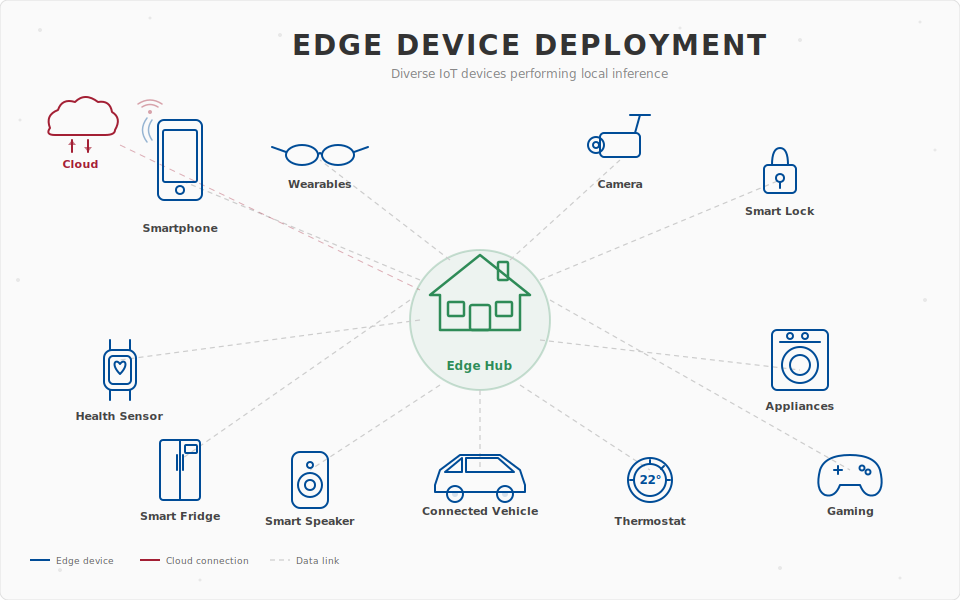
\includegraphics[keepaspectratio]{contents/core/ml_systems/images/jpg/edge_ml_iot.jpg}}

}

\end{figure}%

\textbf{Local Data Storage and Computation}

Local data storage and computation are key features of Edge ML. This
setup ensures that data can be stored and analyzed directly on the
devices, thereby maintaining the privacy of the data and reducing the
need for constant internet connectivity. Moreover, this often leads to
more efficient computation, as data doesn't have to travel long
distances, and computations are performed with a more nuanced
understanding of the local context, which can sometimes result in more
insightful analyses.

\subsection{Benefits}\label{benefits-1}

\textbf{Reduced Latency}

One of Edge ML's main advantages is the significant latency reduction
compared to Cloud ML. This reduced latency can be a critical benefit in
situations where milliseconds count, such as in autonomous vehicles,
where quick decision-making can mean the difference between safety and
an accident.

\textbf{Enhanced Data Privacy}

Edge ML also offers improved data privacy, as data is primarily stored
and processed locally. This minimizes the risk of data breaches that are
more common in centralized data storage solutions. Sensitive information
can be kept more secure, as it's not sent over networks that could be
intercepted.

\textbf{Lower Bandwidth Usage}

Operating closer to the data source means less data must be sent over
networks, reducing bandwidth usage. This can result in cost savings and
efficiency gains, especially in environments where bandwidth is limited
or costly.

\subsection{Challenges}\label{challenges-1}

\textbf{Limited Computational Resources Compared to Cloud ML}

However, Edge ML has its challenges. One of the main concerns is the
limited computational resources compared to cloud-based solutions.
Endpoint devices may have a different processing power or storage
capacity than cloud servers, limiting the complexity of the machine
learning models that can be deployed.

\textbf{Complexity in Managing Edge Nodes}

Managing a network of \textbf{edge nodes}\sidenote{\footnotesize An edge node is a
  computing that acts as a bridge between a local device and the cloud.
  \textbf{Security Concerns at the Edge Nodes}} can introduce
complexity, especially regarding coordination, updates, and maintenance.
Ensuring all nodes operate seamlessly and are up-to-date with the latest
algorithms and security protocols can be a logistical challenge.

While Edge ML offers enhanced data privacy, edge nodes can sometimes be
more vulnerable to physical and cyber-attacks. Developing robust
security protocols that protect data at each node without compromising
the system's efficiency remains a significant challenge in deploying
Edge ML solutions.

\subsection{Example Use Cases}\label{example-use-cases-1}

Edge ML has many applications, from autonomous vehicles and smart homes
to industrial Internet of Things (IoT). These examples were chosen to
highlight scenarios where real-time data processing, reduced latency,
and enhanced privacy are not just beneficial but often critical to the
operation and success of these technologies. They demonstrate the role
that Edge ML can play in driving advancements in various sectors,
fostering innovation, and paving the way for more intelligent,
responsive, and adaptive systems.

\textbf{Autonomous Vehicles}

Autonomous vehicles stand as a prime example of Edge ML's potential.
These vehicles rely heavily on real-time data processing to navigate and
make decisions. Localized machine learning models assist in quickly
analyzing data from various sensors to make immediate driving decisions,
ensuring safety and smooth operation.

\textbf{Smart Homes and Buildings}

Edge ML plays a crucial role in efficiently managing various systems in
smart homes and buildings, from lighting and heating to security. By
processing data locally, these systems can operate more responsively and
harmoniously with the occupants' habits and preferences, creating a more
comfortable living environment.

\textbf{Industrial IoT}

The \textbf{Industrial IoT}\sidenote{\footnotesize Industrial Iot refers to the
  ecosystem of physical devices in an industrial environment that use
  the internet to collect and analyze data.} leverages Edge ML to
monitor and control complex industrial processes. Here, machine learning
models can analyze data from numerous sensors in real-time, enabling
predictive maintenance, optimizing operations, and enhancing safety
measures. This revolution in industrial automation and efficiency is
transforming manufacturing and production across various sectors.

The applicability of Edge ML is vast and not limited to these examples.
Various other sectors, including healthcare, agriculture, and urban
planning, are exploring and integrating Edge ML to develop innovative
solutions responsive to real-world needs and challenges, heralding a new
era of smart, interconnected systems.

\section{Tiny ML}\label{tiny-ml}

\subsection{Characteristics}\label{characteristics-2}

\textbf{Definition of TinyML}

TinyML sits at the crossroads of embedded systems and machine learning,
representing a burgeoning field that brings smart algorithms directly to
tiny microcontrollers and sensors. These microcontrollers operate under
severe resource constraints, particularly regarding memory, storage, and
computational power. Figure~\ref{fig-tiny-ml} encapsulates the key
aspects of TinyML discussed in this section.

\begin{figure}

\sidecaption{\label{fig-tiny-ml}Section overview for Tiny ML.}

\centering{

\pandocbounded{\includegraphics[keepaspectratio]{contents/core/ml_systems/images/png/tinyml.png}}

}

\end{figure}%

\textbf{On-Device Machine Learning}

In TinyML, the focus is on on-device machine learning. This means that
machine learning models are deployed and trained on the device,
eliminating the need for external servers or cloud infrastructures. This
allows TinyML to enable intelligent decision-making right where the data
is generated, making real-time insights and actions possible, even in
settings where connectivity is limited or unavailable.

\textbf{Low Power and Resource-Constrained Environments}

TinyML excels in low-power and resource-constrained settings. These
environments require highly optimized solutions that function within the
available resources. Figure~\ref{fig-tinyml-example} showcases an
example TinyML device kit, illustrating the compact nature of these
systems. These devices can typically fit in the palm of your hand or, in
some cases, are even as small as a fingernail. TinyML meets the need for
efficiency through specialized algorithms and models designed to deliver
decent performance while consuming minimal energy, thus ensuring
extended operational periods, even in battery-powered devices like those
shown.

\begin{figure}

\sidecaption{\label{fig-tinyml-example}Examples of TinyML device kits.
Source: \href{https://arxiv.org/pdf/2106.04008.pdf}{Widening Access to
Applied Machine Learning with TinyML.}}

\centering{

\pandocbounded{\includegraphics[keepaspectratio]{contents/core/ml_systems/images/jpg/tiny_ml.jpg}}

}

\end{figure}%

\begin{tcolorbox}[enhanced jigsaw, bottomtitle=1mm, opacityback=0, colback=white, colframe=quarto-callout-caution-color-frame, toptitle=1mm, toprule=.15mm, breakable, leftrule=.75mm, titlerule=0mm, coltitle=black, left=2mm, bottomrule=.15mm, colbacktitle=quarto-callout-caution-color!10!white, title=\textcolor{quarto-callout-caution-color}{\faFire}\hspace{0.5em}{Caution \ref*{exr-tinyml}: TinyML with Arduino}, arc=.35mm, rightrule=.15mm, opacitybacktitle=0.6]

\quartocalloutexr{exr-tinyml} 

Get ready to bring machine learning to the smallest of devices! In the
embedded machine learning world, TinyML is where resource constraints
meet ingenuity. This Colab notebook will walk you through building a
gesture recognition model designed on an Arduino board. You'll learn how
to train a small but effective neural network, optimize it for minimal
memory usage, and deploy it to your microcontroller. If you're excited
about making everyday objects smarter, this is where it begins!

\href{https://colab.research.google.com/github/arduino/ArduinoTensorFlowLiteTutorials/blob/master/GestureToEmoji/arduino_tinyml_workshop.ipynb}{\pandocbounded{\includegraphics[keepaspectratio]{index_files/mediabag/colab-badge.png}}}

\end{tcolorbox}

\subsection{Benefits}\label{benefits-2}

\textbf{Extremely Low Latency}

One of the standout benefits of TinyML is its ability to offer ultra-low
latency. Since computation occurs directly on the device, the time
required to send data to external servers and receive a response is
eliminated. This is crucial in applications requiring immediate
decision-making, enabling quick responses to changing conditions.

\textbf{High Data Security}

TinyML inherently enhances data security. Because data processing and
analysis happen on the device, the risk of data interception during
transmission is virtually eliminated. This localized approach to data
management ensures that sensitive information stays on the device,
strengthening user data security.

\textbf{Energy Efficiency}

TinyML operates within an energy-efficient framework, a necessity given
its resource-constrained environments. By employing lean algorithms and
optimized computational methods, TinyML ensures that devices can execute
complex tasks without rapidly depleting battery life, making it a
sustainable option for long-term deployments.

\subsection{Challenges}\label{challenges-2}

\textbf{Limited Computational Capabilities}

However, the shift to TinyML comes with its set of hurdles. The primary
limitation is the devices' constrained computational capabilities. The
need to operate within such limits means that deployed models must be
simplified, which could affect the accuracy and sophistication of the
solutions.

\textbf{Complex Development Cycle}

TinyML also introduces a complicated development cycle. Crafting
lightweight and effective models demands a deep understanding of machine
learning principles and expertise in embedded systems. This complexity
calls for a collaborative development approach, where multi-domain
expertise is essential for success.

\textbf{Model Optimization and Compression}

A central challenge in TinyML is model optimization and
compression\sidenote{\footnotesize Model compressions decreases the size of a ML model
  in order to reduce computational power and storage. Popular techniques
  include pruning, quantization, and knowledge distillation.}. Creating
machine learning models that can operate effectively within the limited
memory and computational power of microcontrollers requires innovative
approaches to model design. Developers often face the challenge of
striking a delicate balance and optimizing models to maintain
effectiveness while fitting within stringent resource constraints.

\subsection{Example Use Cases}\label{example-use-cases-2}

\textbf{Wearable Devices}

In wearables, TinyML opens the door to smarter, more responsive gadgets.
From fitness trackers offering real-time workout feedback to smart
glasses processing visual data on the fly, TinyML transforms how we
engage with wearable tech, delivering personalized experiences directly
from the device.

\textbf{Predictive Maintenance}

In industrial settings, TinyML plays a significant role in predictive
maintenance. By deploying TinyML algorithms on sensors that monitor
equipment health, companies can preemptively identify potential issues,
reducing downtime and preventing costly breakdowns. On-site data
analysis ensures quick responses, potentially stopping minor issues from
becoming major problems.

\textbf{Anomaly Detection}

TinyML can be employed to create anomaly detection models that identify
unusual data patterns. For instance, a smart factory could use TinyML to
monitor industrial processes and spot anomalies, helping prevent
accidents and improve product quality. Similarly, a security company
could use TinyML to monitor network traffic for unusual patterns, aiding
in detecting and preventing cyber-attacks. TinyML could monitor patient
data for anomalies in healthcare, aiding early disease detection and
better patient treatment.

\textbf{Environmental Monitoring}

In environmental monitoring, TinyML enables real-time data analysis from
various field-deployed sensors. These could range from city air quality
monitoring to wildlife tracking in protected areas. Through TinyML, data
can be processed locally, allowing for quick responses to changing
conditions and providing a nuanced understanding of environmental
patterns, crucial for informed decision-making.

In summary, TinyML serves as a trailblazer in the evolution of machine
learning, fostering innovation across various fields by bringing
intelligence directly to the edge. Its potential to transform our
interaction with technology and the world is immense, promising a future
where devices are connected, intelligent, and capable of making
real-time decisions and responses.

\section{Comparison}\label{comparison}

Let's bring together the different ML variants we've explored
individually for a comprehensive view. Figure~\ref{fig-venn-diagram}
illustrates the relationships and overlaps between Cloud ML, Edge ML,
and TinyML using a Venn diagram. This visual representation effectively
highlights the unique characteristics of each approach while also
showing areas of commonality. Each ML paradigm has its own distinct
features, but there are also intersections where these approaches share
certain attributes or capabilities. This diagram helps us understand how
these variants relate to each other in the broader landscape of machine
learning implementations.

\begin{figure}

\sidecaption{\label{fig-venn-diagram}ML Venn diagram. Source:
\href{https://arxiv.org/html/2403.19076v1}{arXiv}}

\centering{

\pandocbounded{\includegraphics[keepaspectratio]{contents/core/ml_systems/images/png/venndiagram.png}}

}

\end{figure}%

For a more detailed comparison of these ML variants, we can refer to
Table~\ref{tbl-big_vs_tiny}. This table offers a comprehensive analysis
of Cloud ML, Edge ML, and TinyML based on various features and aspects.
By examining these different characteristics side by side, we gain a
clearer perspective on the unique advantages and distinguishing factors
of each approach. This detailed comparison, combined with the visual
overview provided by the Venn diagram, aids in making informed decisions
based on the specific needs and constraints of a given application or
project.

\begin{longtable}[]{@{}
  >{\raggedright\arraybackslash}p{(\linewidth - 6\tabcolsep) * \real{0.1324}}
  >{\raggedright\arraybackslash}p{(\linewidth - 6\tabcolsep) * \real{0.2843}}
  >{\raggedright\arraybackslash}p{(\linewidth - 6\tabcolsep) * \real{0.2843}}
  >{\raggedright\arraybackslash}p{(\linewidth - 6\tabcolsep) * \real{0.2892}}@{}}
\caption{Comparison of feature aspects across Cloud ML, Edge ML, and
TinyML.}\label{tbl-big_vs_tiny}\tabularnewline
\toprule\noalign{}
\begin{minipage}[b]{\linewidth}\raggedright
Aspect
\end{minipage} & \begin{minipage}[b]{\linewidth}\raggedright
Cloud ML
\end{minipage} & \begin{minipage}[b]{\linewidth}\raggedright
Edge ML
\end{minipage} & \begin{minipage}[b]{\linewidth}\raggedright
TinyML
\end{minipage} \\
\midrule\noalign{}
\endfirsthead
\toprule\noalign{}
\begin{minipage}[b]{\linewidth}\raggedright
Aspect
\end{minipage} & \begin{minipage}[b]{\linewidth}\raggedright
Cloud ML
\end{minipage} & \begin{minipage}[b]{\linewidth}\raggedright
Edge ML
\end{minipage} & \begin{minipage}[b]{\linewidth}\raggedright
TinyML
\end{minipage} \\
\midrule\noalign{}
\endhead
\bottomrule\noalign{}
\endlastfoot
Processing Location & Centralized servers (Data Centers) & Local devices
(closer to data sources) & On-device (microcontrollers, embedded
systems) \\
Latency & High (Depends on internet connectivity) & Moderate (Reduced
latency compared to Cloud ML) & Low (Immediate processing without
network delay) \\
Data Privacy & Moderate (Data transmitted over networks) & High (Data
remains on local networks) & Very High (Data processed on-device, not
transmitted) \\
Computational Power & High (Utilizes powerful data center
infrastructure) & Moderate (Utilizes local device capabilities) & Low
(Limited to the power of the embedded system) \\
Energy Consumption & High (Data centers consume significant energy) &
Moderate (Less than data centers, more than TinyML) & Low (Highly
energy-efficient, designed for low power) \\
Scalability & High (Easy to scale with additional server resources) &
Moderate (Depends on local device capabilities) & Low (Limited by the
hardware resources of the device) \\
Cost & High (Recurring costs for server usage, maintenance) & Variable
(Depends on the complexity of local setup) & Low (Primarily upfront
costs for hardware components) \\
Connectivity & High (Requires stable internet connectivity) & Low (Can
operate with intermittent connectivity) & Very Low (Can operate without
any network connectivity) \\
Real-time Processing & Moderate (Can be affected by network latency) &
High (Capable of real-time processing locally) & Very High (Immediate
processing with minimal latency) \\
Application Examples & Big Data Analysis, Virtual Assistants &
Autonomous Vehicles, Smart Homes & Wearables, Sensor Networks \\
Complexity & Moderate to High (Requires knowledge in cloud computing) &
Moderate (Requires knowledge in local network setup) & Moderate to High
(Requires expertise in embedded systems) \\
\end{longtable}

\section{Conclusion}\label{conclusion}

In this chapter, we've offered a panoramic view of the evolving
landscape of machine learning, covering cloud, edge, and tiny ML
paradigms. Cloud-based machine learning leverages the immense
computational resources of cloud platforms to enable powerful and
accurate models but comes with limitations, including latency and
privacy concerns. Edge ML mitigates these limitations by bringing
inference directly to edge devices, offering lower latency and reduced
connectivity needs. TinyML takes this further by miniaturizing ML models
to run directly on highly resource-constrained devices, opening up a new
category of intelligent applications.

Each approach has its tradeoffs, including model complexity, latency,
privacy, and hardware costs. Over time, we anticipate converging these
embedded ML approaches, with cloud pre-training facilitating more
sophisticated edge and tiny ML implementations. Advances like federated
learning and on-device learning will enable embedded devices to refine
their models by learning from real-world data.

The embedded ML landscape is rapidly evolving and poised to enable
intelligent applications across a broad spectrum of devices and use
cases. This chapter serves as a snapshot of the current state of
embedded ML. As algorithms, hardware, and connectivity continue to
improve, we can expect embedded devices of all sizes to become
increasingly capable, unlocking transformative new applications for
artificial intelligence.

\section{Resources}\label{sec-ml-systems-resource}

Here is a curated list of resources to support students and instructors
in their learning and teaching journeys. We are continuously working on
expanding this collection and will be adding new exercises soon.

\begin{tcolorbox}[enhanced jigsaw, bottomtitle=1mm, opacityback=0, colback=white, colframe=quarto-callout-note-color-frame, toptitle=1mm, toprule=.15mm, breakable, leftrule=.75mm, titlerule=0mm, coltitle=black, left=2mm, bottomrule=.15mm, colbacktitle=quarto-callout-note-color!10!white, title=\textcolor{quarto-callout-note-color}{\faInfo}\hspace{0.5em}{Slides}, arc=.35mm, rightrule=.15mm, opacitybacktitle=0.6]

These slides are a valuable tool for instructors to deliver lectures and
for students to review the material at their own pace. We encourage
students and instructors to leverage these slides to improve their
understanding and facilitate effective knowledge transfer.

\begin{itemize}
\item
  \href{https://docs.google.com/presentation/d/1Lgrn7bddHYxyrOmk0JfSVmEBimRePqI7WSliUKRPK9E/edit?resourcekey=0-c5JvfDeqHIdV9A5RMAMAyw\#slide=id.g94db9f9f78_0_8}{Embedded
  Systems Overview.}
\item
  \href{https://docs.google.com/presentation/d/1hDCFcOrZ08kZPhY4DA3gVikGUo47HwNyvqNrLW-t-Tg/edit?resourcekey=0-J6ix5AYvZMGbFFOa7ae4Hw\#slide=id.g94db9f9f78_0_8}{Embedded
  Computer Hardware.}
\item
  \href{https://docs.google.com/presentation/d/1rnWh9XC6iCKSx_hQd4xq2iIDlpc-GkBQw_GjzlP5mQc/edit\#slide=id.g94db9f9f78_0_8}{Embedded
  I/O.}
\item
  \href{https://docs.google.com/presentation/d/1TApZn9xxPWCRY-D-soJ8YOSsfysnccR5UjOyspzeTuU/edit?resourcekey=0-BRWIyCKPLNQFnIfG0fJJ9A\#slide=id.g94db9f9f78_0_8}{Embedded
  systems software.}
\item
  \href{https://docs.google.com/presentation/d/17wgAfoF24Rcx7uPrbau0c8FyzXIUWbe48qGGBOXXT-g/edit?resourcekey=0-Uv29DvmF7gYzKdOoRtn0vw\#slide=id.g94db9f9f78_0_8}{Embedded
  ML software.}
\item
  \href{https://docs.google.com/presentation/d/1FOUQ9dbe3l_qTa2AnroSbOz0ykuCz5cbTNO77tvFxEs/edit?usp=drive_link}{Embedded
  Inference.}
\item
  \href{https://docs.google.com/presentation/d/1jwAZz3UOoJTR8PY6Wa34FxijpoDc9gBM/edit?usp=drive_link&ouid=102419556060649178683&rtpof=true&sd=true}{TinyML
  on Microcontrollers.}
\item
  TinyML as a Service (TinyMLaaS):

  \begin{itemize}
  \item
    \href{https://docs.google.com/presentation/d/1O7bxb36SnexfDI3iE_p0C8JI_VYXAL8cyAx3JKDfeUo/edit?usp=drive_link}{TinyMLaaS:
    Introduction.}
  \item
    \href{https://docs.google.com/presentation/d/1ZUUHtTbKlzeTwVteQMSztscQmdmMxT1A24pBKSys7g0/edit\#slide=id.g94db9f9f78_0_2}{TinyMLaaS:
    Design Overview.}
  \end{itemize}
\end{itemize}

\end{tcolorbox}

\begin{tcolorbox}[enhanced jigsaw, bottomtitle=1mm, opacityback=0, colback=white, colframe=quarto-callout-important-color-frame, toptitle=1mm, toprule=.15mm, breakable, leftrule=.75mm, titlerule=0mm, coltitle=black, left=2mm, bottomrule=.15mm, colbacktitle=quarto-callout-important-color!10!white, title=\textcolor{quarto-callout-important-color}{\faExclamation}\hspace{0.5em}{Videos}, arc=.35mm, rightrule=.15mm, opacitybacktitle=0.6]

\begin{itemize}
\tightlist
\item
  \emph{Coming soon.}
\end{itemize}

\end{tcolorbox}

\begin{tcolorbox}[enhanced jigsaw, bottomtitle=1mm, opacityback=0, colback=white, colframe=quarto-callout-caution-color-frame, toptitle=1mm, toprule=.15mm, breakable, leftrule=.75mm, titlerule=0mm, coltitle=black, left=2mm, bottomrule=.15mm, colbacktitle=quarto-callout-caution-color!10!white, title=\textcolor{quarto-callout-caution-color}{\faFire}\hspace{0.5em}{Exercises}, arc=.35mm, rightrule=.15mm, opacitybacktitle=0.6]

To reinforce the concepts covered in this chapter, we have curated a set
of exercises that challenge students to apply their knowledge and deepen
their understanding.

\begin{itemize}
\tightlist
\item
  \emph{Coming soon.}
\end{itemize}

\end{tcolorbox}

\begin{tcolorbox}[enhanced jigsaw, bottomtitle=1mm, opacityback=0, colback=white, colframe=quarto-callout-warning-color-frame, toptitle=1mm, toprule=.15mm, breakable, leftrule=.75mm, titlerule=0mm, coltitle=black, left=2mm, bottomrule=.15mm, colbacktitle=quarto-callout-warning-color!10!white, title=\textcolor{quarto-callout-warning-color}{\faExclamationTriangle}\hspace{0.5em}{Labs}, arc=.35mm, rightrule=.15mm, opacitybacktitle=0.6]

In addition to exercises, we offer a series of hands-on labs allowing
students to gain practical experience with embedded AI technologies.
These labs provide step-by-step guidance, enabling students to develop
their skills in a structured and supportive environment. We are excited
to announce that new labs will be available soon, further enriching the
learning experience.

\begin{itemize}
\tightlist
\item
  \emph{Coming soon.}
\end{itemize}

\end{tcolorbox}

\bookmarksetup{startatroot}

\chapter{DL Primer}\label{sec-dl_primer}

\begin{figure}[H]

\sidecaption{\emph{DALL·E 3 Prompt: Photo of a classic classroom with a
large blackboard dominating one wall. Chalk drawings showcase a detailed
deep neural network with several hidden layers, and each node and
connection is precisely labeled with white chalk. The rustic wooden
floor and brick walls provide a contrast to the modern concepts.
Surrounding the room, posters mounted on frames emphasize deep learning
themes: convolutional networks, transformers, neurons, activation
functions, and more.}}

{\centering \pandocbounded{\includegraphics[keepaspectratio]{contents/core/dl_primer/images/png/cover_dl_primer.png}}

}

\end{figure}%

This section serves as a primer for deep learning, providing systems
practitioners with essential context and foundational knowledge needed
to implement deep learning solutions effectively. Rather than delving
into theoretical depths, we focus on key concepts, architectures, and
practical considerations relevant to systems implementation. We begin
with an overview of deep learning's evolution and its particular
significance in embedded AI systems. Core concepts like neural networks
are introduced with an emphasis on implementation considerations rather
than mathematical foundations.

The primer explores major deep learning architectures from a systems
perspective, examining their practical implications and resource
requirements. We also compare deep learning to traditional machine
learning approaches, helping readers make informed architectural choices
based on real-world system constraints. This high-level overview sets
the context for the more detailed systems-focused techniques and
optimizations covered in subsequent chapters.

\begin{tcolorbox}[enhanced jigsaw, bottomtitle=1mm, opacityback=0, colback=white, colframe=quarto-callout-tip-color-frame, toptitle=1mm, toprule=.15mm, breakable, leftrule=.75mm, titlerule=0mm, coltitle=black, left=2mm, bottomrule=.15mm, colbacktitle=quarto-callout-tip-color!10!white, title=\textcolor{quarto-callout-tip-color}{\faLightbulb}\hspace{0.5em}{Learning Objectives}, arc=.35mm, rightrule=.15mm, opacitybacktitle=0.6]

\begin{itemize}
\item
  Understand the basic concepts and definitions of deep neural networks.
\item
  Recognize there are different deep learning model architectures.
\item
  Comparison between deep learning and traditional machine learning
  approaches across various dimensions.
\item
  Acquire the basic conceptual building blocks to dive deeper into
  advanced deep-learning techniques and applications.
\end{itemize}

\end{tcolorbox}

\section{Introduction}\label{introduction-1}

\subsection{Definition and Importance}\label{definition-and-importance}

Deep learning, a specialized area within machine learning and artificial
intelligence (AI), utilizes algorithms modeled after the structure and
function of the human brain, known as artificial neural networks. This
field is a foundational element in AI, driving progress in diverse
sectors such as computer vision, natural language processing, and
self-driving vehicles. Its significance in embedded AI systems is
highlighted by its capability to handle intricate calculations and
predictions, optimizing the limited resources in embedded settings.

Figure~\ref{fig-ai-ml-dl} provides a visual representation of how deep
learning fits within the broader context of AI and machine learning. The
diagram illustrates the chronological development and relative
segmentation of these three interconnected fields, showcasing deep
learning as a specialized subset of machine learning, which in turn is a
subset of AI.

\begin{figure}

\sidecaption{\label{fig-ai-ml-dl}The diagram illustrates artificial
intelligence as the overarching field encompassing all computational
methods that mimic human cognitive functions. Machine learning is a
subset of AI that includes algorithms capable of learning from data.
Deep learning, a further subset of ML, specifically involves neural
networks that are able to learn more complex patterns in large volumes
of data. Source: NVIDIA.}

\centering{

\pandocbounded{\includegraphics[keepaspectratio]{contents/core/dl_primer/images/png/ai_dl_progress_nvidia.png}}

}

\end{figure}%

As shown in the figure, AI represents the overarching field,
encompassing all computational methods that mimic human cognitive
functions. Machine learning, shown as a subset of AI, includes
algorithms capable of learning from data. Deep learning, the smallest
subset in the diagram, specifically involves neural networks that are
able to learn more complex patterns from large volumes of data.

\subsection{Brief History of Deep
Learning}\label{brief-history-of-deep-learning}

The idea of deep learning has origins in early artificial neural
networks. It has experienced several cycles of interest, starting with
the introduction of the Perceptron in the 1950s
(\citeproc{ref-rosenblatt1957perceptron}{Rosenblatt 1957}), followed by
the invention of backpropagation algorithms in the 1980s
(\citeproc{ref-rumelhart1986learning}{Rumelhart, Hinton, and Williams
1986}).

The term ``deep learning'' became prominent in the 2000s, characterized
by advances in computational power and data accessibility. Important
milestones include the successful training of deep networks like AlexNet
(\citeproc{ref-krizhevsky2012imagenet}{Krizhevsky, Sutskever, and Hinton
2012}) by
\href{https://amturing.acm.org/award_winners/hinton_4791679.cfm}{Geoffrey
Hinton}, a leading figure in AI, and the renewed focus on neural
networks as effective tools for data analysis and modeling.

Deep learning has recently seen exponential growth, transforming various
industries. Figure~\ref{fig-trends} illustrates this remarkable
progression, highlighting two key trends in the field. First, the graph
shows that computational growth followed an 18-month doubling pattern
from 1952 to 2010. This trend then dramatically accelerated to a 6-month
doubling cycle from 2010 to 2022, indicating a significant leap in
computational capabilities.

Second, the figure depicts the emergence of large-scale models between
2015 and 2022. These models appeared 2 to 3 orders of magnitude faster
than the general trend, following an even more aggressive 10-month
doubling cycle. This rapid scaling of model sizes represents a paradigm
shift in deep learning capabilities.

\begin{figure}

\sidecaption{\label{fig-trends}Growth of deep learning models.}

\centering{

\pandocbounded{\includegraphics[keepaspectratio]{index_files/mediabag/compute-trends.png}}

}

\end{figure}%

Multiple factors have contributed to this surge, including advancements
in computational power, the abundance of big data, and improvements in
algorithmic designs. First, the growth of computational capabilities,
especially the arrival of Graphics Processing Units (GPUs) and Tensor
Processing Units (TPUs) (\citeproc{ref-jouppi2017datacenter}{N. P.
Jouppi et al. 2017a}), has significantly sped up the training and
inference times of deep learning models. These hardware improvements
have enabled the construction and training of more complex, deeper
networks than what was possible in earlier years.

Second, the digital revolution has yielded a wealth of big data,
offering rich material for deep learning models to learn from and excel
in tasks such as image and speech recognition, language translation, and
game playing. Large, labeled datasets have been key in refining and
successfully deploying deep learning applications in real-world
settings.

Additionally, collaborations and open-source efforts have nurtured a
dynamic community of researchers and practitioners, accelerating
advancements in deep learning techniques. Innovations like deep
reinforcement learning, transfer learning, and generative artificial
intelligence have broadened the scope of what is achievable with deep
learning, opening new possibilities in various sectors, including
healthcare, finance, transportation, and entertainment.

Organizations worldwide recognize deep learning's transformative
potential and invest heavily in research and development to leverage its
capabilities in providing innovative solutions, optimizing operations,
and creating new business opportunities. As deep learning continues its
upward trajectory, it is set to redefine how we interact with
technology, enhancing convenience, safety, and connectivity in our
lives.

\subsection{Applications of Deep
Learning}\label{applications-of-deep-learning}

Deep learning is extensively used across numerous industries today, with
its transformative impact evident in various sectors, as illustrated in
Figure~\ref{fig-deeplearning}. In finance, it powers stock market
prediction, risk assessment, and fraud detection, guiding investment
strategies and improving financial decisions. Marketing leverages deep
learning for customer segmentation and personalization, enabling highly
targeted advertising and content optimization based on consumer behavior
analysis. In manufacturing, it streamlines production processes and
enhances quality control, allowing companies to boost productivity and
minimize waste. Healthcare benefits from deep learning in diagnosis,
treatment planning, and patient monitoring, potentially saving lives
through improved medical predictions.

\begin{figure}

\sidecaption{\label{fig-deeplearning}Deep learning applications,
benefits, and implementations across various industries including
finance, marketing, manufacturing, and healthcare. Source:
\href{https://www.leewayhertz.com/what-is-deep-learning/}{Leeway Hertz}}

\centering{

\pandocbounded{\includegraphics[keepaspectratio]{contents/core/dl_primer/images/png/deeplearning.png}}

}

\end{figure}%

Beyond these core industries, deep learning enhances everyday products
and services. Netflix uses it to strengthen its recommender systems,
providing users with more
\href{https://dl.acm.org/doi/abs/10.1145/3543873.3587675}{personalized
recommendations}. Google has significantly improved its Translate
service, now handling over
\href{https://cloud.google.com/translate/docs/languages}{100 languages}
with increased accuracy, as highlighted in their
\href{https://research.google/blog/recent-advances-in-google-translate/}{recent
advances}. Autonomous vehicles from companies like Waymo, Cruise, and
Motional have become a reality through deep learning in their
\href{https://motional.com/news/technically-speaking-improving-av-perception-through-transformative-machine-learning}{perception
system}. Additionally, Amazon employs deep learning at the edge in Alexa
devices for tasks such as
\href{https://towardsdatascience.com/how-amazon-alexa-works-your-guide-to-natural-language-processing-ai-7506004709d3}{keyword
spotting}. These applications demonstrate how machine learning often
predicts and processes information with greater accuracy and speed than
humans, revolutionizing various aspects of our daily lives.

\subsection{Relevance to Embedded AI}\label{relevance-to-embedded-ai}

Embedded AI, the integration of AI algorithms directly into hardware
devices, naturally gains from deep learning capabilities. Combining deep
learning algorithms and embedded systems has laid the groundwork for
intelligent, autonomous devices capable of advanced on-device data
processing and analysis. Deep learning aids in extracting complex
patterns and information from input data, which is essential in
developing smart embedded systems, from household appliances to
industrial machinery. This collaboration ushers in a new era of
intelligent, interconnected devices that can learn and adapt to user
behavior and environmental conditions, optimizing performance and
offering unprecedented convenience and efficiency.

\section{Neural Networks}\label{neural-networks}

Deep learning draws inspiration from the human brain's neural networks
to create decision-making patterns. This section digs into the
foundational concepts of deep learning, providing insights into the more
complex topics discussed later in this primer.

Neural networks serve as the foundation of deep learning, inspired by
the biological neural networks in the human brain to process and analyze
data hierarchically. Neural networks are composed of basic units called
perceptrons, which are typically organized into layers. Each layer
consists of several perceptrons, and multiple layers are stacked to form
the entire network. The connections between these layers are defined by
sets of weights or parameters that determine how data is processed as it
flows from the input to the output of the network.

Below, we examine the primary components and structures in neural
networks.

\subsection{Perceptrons}\label{perceptrons}

The Perceptron is the basic unit or node that forms the foundation for
more complex structures. It functions by taking multiple inputs, each
representing a feature of the object under analysis, such as the
characteristics of a home for predicting its price or the attributes of
a song to forecast its popularity in music streaming services. These
inputs are denoted as \(x_1, x_2, ..., x_n\). A perceptron can be
configured to perform either regression or classification tasks. For
regression, the actual numerical output \(\hat{y}\) is used. For
classification, the output depends on whether \(\hat{y}\) crosses a
certain threshold. If \(\hat{y}\) exceeds this threshold, the perceptron
might output one class (e.g., `yes'), and if it does not, another class
(e.g., `no').

Figure~\ref{fig-perceptron} illustrates the fundamental building blocks
of a perceptron, which serves as the foundation for more complex neural
networks. A perceptron can be thought of as a miniature decision-maker,
utilizing its weights, bias, and activation function to process inputs
and generate outputs based on learned parameters. This concept forms the
basis for understanding more intricate neural network architectures,
such as multilayer perceptrons. In these advanced structures, layers of
perceptrons work in concert, with each layer's output serving as the
input for the subsequent layer. This hierarchical arrangement creates a
deep learning model capable of comprehending and modeling complex,
abstract patterns within data. By stacking these simple units, neural
networks gain the ability to tackle increasingly sophisticated tasks,
from image recognition to natural language processing.

\begin{figure}

\sidecaption{\label{fig-perceptron}Perceptron. Conceived in the 1950s,
perceptrons paved the way for developing more intricate neural networks
and have been a fundamental building block in deep learning. Source:
Wikimedia - Chrislb.}

\centering{

\pandocbounded{\includegraphics[keepaspectratio]{contents/core/dl_primer/images/png/Rosenblattperceptron.png}}

}

\end{figure}%

Each input \(x_i\) has a corresponding weight \(w_{ij}\), and the
perceptron simply multiplies each input by its matching weight. This
operation is similar to linear regression, where the intermediate
output, \(z\), is computed as the sum of the products of inputs and
their weights:

\[
z = \sum (x_i \cdot w_{ij})
\]

To this intermediate calculation, a bias term \(b\) is added, allowing
the model to better fit the data by shifting the linear output function
up or down. Thus, the intermediate linear combination computed by the
perceptron including the bias becomes:

\[
z = \sum (x_i \cdot w_{ij}) + b
\]

This basic form of a perceptron can only model linear relationships
between the input and output. Patterns found in nature are often complex
and extend beyond linear relationships. To enable the perceptron to
handle non-linear relationships, an activation function is applied to
the linear output \(z\).

\[
\hat{y} = \sigma(z)
\]

Figure~\ref{fig-nonlinear} illustrates an example where data exhibit a
nonlinear pattern that could not be adequately modeled with a linear
approach. The activation function, such as sigmoid, tanh, or ReLU,
transforms the linear input sum into a non-linear output. The primary
objective of this function is to introduce non-linearity into the model,
enabling it to learn and perform more sophisticated tasks. Thus, the
final output of the perceptron, including the activation function, can
be expressed as:

\begin{figure}

\sidecaption{\label{fig-nonlinear}Activation functions enable the
modeling of complex non-linear relationships. Source: Medium - Sachin
Kaushik.}

\centering{

\pandocbounded{\includegraphics[keepaspectratio]{contents/core/dl_primer/images/png/nonlinear_patterns.png}}

}

\end{figure}%

\subsection{Multilayer Perceptrons}\label{multilayer-perceptrons}

Multilayer perceptrons (MLPs) are an evolution of the single-layer
perceptron model, featuring multiple layers of nodes connected in a
feedforward manner. Figure~\ref{fig-mlp} provides a visual
representation of this structure. As illustrated in the figure,
information in a feedforward network moves in only one direction - from
the input layer on the left, through the hidden layers in the middle, to
the output layer on the right, without any cycles or loops.

\begin{figure}

\sidecaption{\label{fig-mlp}Multilayer Perceptron. Source: Wikimedia -
Charlie.}

\centering{

\includegraphics[width=0.7\linewidth,height=\textheight,keepaspectratio]{index_files/mediabag/image-7.png}

}

\end{figure}%

While a single perceptron is limited in its capacity to model complex
patterns, the real strength of neural networks emerges from the assembly
of multiple layers. Each layer consists of numerous perceptrons working
together, allowing the network to capture intricate and non-linear
relationships within the data. With sufficient depth and breadth, these
networks can approximate virtually any function, no matter how complex.

\subsection{Training Process}\label{training-process}

A neural network receives an input, performs a calculation, and produces
a prediction. The prediction is determined by the calculations performed
within the sets of perceptrons found between the input and output
layers. These calculations depend primarily on the input and the
weights. Since you do not have control over the input, the objective
during training is to adjust the weights in such a way that the output
of the network provides the most accurate prediction.

The training process involves several key steps, beginning with the
forward pass, where the existing weights of the network are used to
calculate the output for a given input. This output is then compared to
the true target values to calculate an error, which measures how well
the network's prediction matches the expected outcome. Following this, a
backward pass is performed. This involves using the error to make
adjustments to the weights of the network through a process called
backpropagation. This adjustment reduces the error in subsequent
predictions. The cycle of forward pass, error calculation, and backward
pass is repeated iteratively. This process continues until the network's
predictions are sufficiently accurate or a predefined number of
iterations is reached, effectively minimizing the loss function used to
measure the error.

\subsubsection{Forward Pass}\label{forward-pass}

The forward pass is the initial phase where data moves through the
network from the input to the output layer, as illustrated in
Figure~\ref{fig-forward-propagation}. At the start of training, the
network's weights are randomly initialized, setting the initial
conditions for learning. During the forward pass, each layer performs
specific computations on the input data using these weights and biases,
and the results are then passed to the subsequent layer. The final
output of this phase is the network's prediction. This prediction is
compared to the actual target values present in the dataset to calculate
the loss, which can be thought of as the difference between the
predicted outputs and the target values. The loss quantifies the
network's performance at this stage, providing a crucial metric for the
subsequent adjustment of weights during the backward pass.

\begin{figure}

\sidecaption{\label{fig-forward-propagation}Neural networks - forward
and backward propagation. Source:
\href{https://www.linkedin.com/pulse/lecture2-unveiling-theoretical-foundations-ai-machine-underdown-phd-oqsuc/}{Linkedin}}

\centering{

\pandocbounded{\includegraphics[keepaspectratio]{contents/core/dl_primer/images/png/forwardpropagation.png}}

}

\end{figure}%

\subsubsection{Backward Pass (Backpropagation)}\label{sec-backward_pass}

After completing the forward pass and computing the loss, which measures
how far the model's predictions deviate from the actual target values,
the next step is to improve the model's performance by adjusting the
network's weights. Since we cannot control the inputs to the model,
adjusting the weights becomes our primary method for refining the model.

We determine how to adjust the weights of our model through a key
algorithm called backpropagation. Backpropagation uses the calculated
loss to determine the gradient of each weight. These gradients describe
the direction and magnitude in which the weights should be adjusted. By
tuning the weights based on these gradients, the model is better
positioned to make predictions that are closer to the actual target
values in the next forward pass.

Grasping these foundational concepts paves the way to understanding more
intricate deep learning architectures and techniques, fostering the
development of more sophisticated and productive applications,
especially within embedded AI systems.

Video~\ref{vid-gd} and Video~\ref{vid-bp} build upon Video~\ref{vid-nn}.
They cover gradient descent and backpropagation in neural networks.

\begin{tcolorbox}[enhanced jigsaw, bottomtitle=1mm, opacityback=0, colback=white, colframe=quarto-callout-important-color-frame, toptitle=1mm, toprule=.15mm, breakable, leftrule=.75mm, titlerule=0mm, coltitle=black, left=2mm, bottomrule=.15mm, colbacktitle=quarto-callout-important-color!10!white, title=\textcolor{quarto-callout-important-color}{\faExclamation}\hspace{0.5em}{Important \ref*{vid-gd}: Gradient descent}, arc=.35mm, rightrule=.15mm, opacitybacktitle=0.6]

\quartocalloutvid{vid-gd} 

\url{https://www.youtube.com/watch?v=IHZwWFHWa-w&list=PLZHQObOWTQDNU6R1_67000Dx_ZCJB-3pi&index=2}

\end{tcolorbox}

\begin{tcolorbox}[enhanced jigsaw, bottomtitle=1mm, opacityback=0, colback=white, colframe=quarto-callout-important-color-frame, toptitle=1mm, toprule=.15mm, breakable, leftrule=.75mm, titlerule=0mm, coltitle=black, left=2mm, bottomrule=.15mm, colbacktitle=quarto-callout-important-color!10!white, title=\textcolor{quarto-callout-important-color}{\faExclamation}\hspace{0.5em}{Important \ref*{vid-bp}: Backpropagation}, arc=.35mm, rightrule=.15mm, opacitybacktitle=0.6]

\quartocalloutvid{vid-bp} 

\url{https://www.youtube.com/watch?v=Ilg3gGewQ5U&list=PLZHQObOWTQDNU6R1_67000Dx_ZCJB-3pi&index=3}

\end{tcolorbox}

\subsection{Model Architectures}\label{model-architectures}

Deep learning architectures refer to the various structured approaches
that dictate how neurons and layers are organized and interact in neural
networks. These architectures have evolved to tackle different problems
and data types effectively. This section overviews some well-known deep
learning architectures and their characteristics.

\subsubsection{Multilayer Perceptrons
(MLPs)}\label{multilayer-perceptrons-mlps}

MLPs are basic deep learning architectures comprising three layers: an
input layer, one or more hidden layers, and an output layer. These
layers are fully connected, meaning each neuron in a layer is linked to
every neuron in the preceding and following layers. MLPs can model
intricate functions and are used in various tasks, such as regression,
classification, and pattern recognition. Their capacity to learn
non-linear relationships through backpropagation makes them a versatile
instrument in the deep learning toolkit.

In embedded AI systems, MLPs can function as compact models for simpler
tasks like sensor data analysis or basic pattern recognition, where
computational resources are limited. Their ability to learn non-linear
relationships with relatively less complexity makes them a suitable
choice for embedded systems.

\begin{tcolorbox}[enhanced jigsaw, bottomtitle=1mm, opacityback=0, colback=white, colframe=quarto-callout-caution-color-frame, toptitle=1mm, toprule=.15mm, breakable, leftrule=.75mm, titlerule=0mm, coltitle=black, left=2mm, bottomrule=.15mm, colbacktitle=quarto-callout-caution-color!10!white, title=\textcolor{quarto-callout-caution-color}{\faFire}\hspace{0.5em}{Caution \ref*{exr-mlp}: Multilayer Perceptrons (MLPs)}, arc=.35mm, rightrule=.15mm, opacitybacktitle=0.6]

\quartocalloutexr{exr-mlp} 

We've just scratched the surface of neural networks. Now, you'll get to
try and apply these concepts in practical examples. In the provided
Colab notebooks, you'll explore:

\textbf{Predicting house prices:}~Learn how neural networks can analyze
housing data to estimate property values.~~
\href{https://colab.research.google.com/github/Mjrovai/UNIFEI-IESTI01-TinyML-2022.1/blob/main/00_Curse_Folder/1_Fundamentals/Class_07/TF_Boston_Housing_Regression.ipynb}{\pandocbounded{\includegraphics[keepaspectratio]{index_files/mediabag/colab-badge.png}}}

\textbf{Image Classification:}~Discover how to build a network to
understand the famous MNIST handwritten digit dataset.~~
\href{https://colab.research.google.com/github/Mjrovai/UNIFEI-IESTI01-TinyML-2022.1/blob/main/00_Curse_Folder/1_Fundamentals/Class_09/TF_MNIST_Classification_v2.ipynb}{\pandocbounded{\includegraphics[keepaspectratio]{index_files/mediabag/colab-badge.png}}}

\textbf{Real-world medical diagnosis:}~Use deep learning to tackle the
important task of breast cancer classification.~~
\href{https://colab.research.google.com/github/Mjrovai/UNIFEI-IESTI01-TinyML-2022.1/blob/main/00_Curse_Folder/1_Fundamentals/Class_13/docs/WDBC_Project/Breast_Cancer_Classification.ipynb}{\pandocbounded{\includegraphics[keepaspectratio]{index_files/mediabag/colab-badge.png}}}

\end{tcolorbox}

\subsubsection{Convolutional Neural Networks
(CNNs)}\label{convolutional-neural-networks-cnns}

CNNs are mainly used in image and video recognition tasks. This
architecture consists of two main parts: the convolutional base and the
fully connected layers. In the convolutional base, convolutional layers
filter input data to identify features like edges, corners, and
textures. Following each convolutional layer, a pooling layer can be
applied to reduce the spatial dimensions of the data, thereby decreasing
computational load and concentrating the extracted features. Unlike
MLPs, which treat input features as flat, independent entities, CNNs
maintain the spatial relationships between pixels, making them
particularly effective for image and video data. The extracted features
from the convolutional base are then passed into the fully connected
layers, similar to those used in MLPs, which perform classification
based on the features extracted by the convolution layers. CNNs have
proven highly effective in image recognition, object detection, and
other computer vision applications.

Video~\ref{vid-nn} explains how neural networks work using handwritten
digit recognition as an example application. It also touches on the math
underlying neural nets.

\begin{tcolorbox}[enhanced jigsaw, bottomtitle=1mm, opacityback=0, colback=white, colframe=quarto-callout-important-color-frame, toptitle=1mm, toprule=.15mm, breakable, leftrule=.75mm, titlerule=0mm, coltitle=black, left=2mm, bottomrule=.15mm, colbacktitle=quarto-callout-important-color!10!white, title=\textcolor{quarto-callout-important-color}{\faExclamation}\hspace{0.5em}{Important \ref*{vid-nn}: MLP \& CNN Networks}, arc=.35mm, rightrule=.15mm, opacitybacktitle=0.6]

\quartocalloutvid{vid-nn} 

\url{https://www.youtube.com/embed/aircAruvnKk?si=ZRj8jf4yx7ZMe8EK}

\end{tcolorbox}

CNNs are crucial for image and video recognition tasks, where real-time
processing is often needed. They can be optimized for embedded systems
using techniques like quantization and pruning to minimize memory usage
and computational demands, enabling efficient object detection and
facial recognition functionalities in devices with limited computational
resources.

\begin{tcolorbox}[enhanced jigsaw, bottomtitle=1mm, opacityback=0, colback=white, colframe=quarto-callout-caution-color-frame, toptitle=1mm, toprule=.15mm, breakable, leftrule=.75mm, titlerule=0mm, coltitle=black, left=2mm, bottomrule=.15mm, colbacktitle=quarto-callout-caution-color!10!white, title=\textcolor{quarto-callout-caution-color}{\faFire}\hspace{0.5em}{Caution \ref*{exr-cnn}: Convolutional Neural Networks (CNNs)}, arc=.35mm, rightrule=.15mm, opacitybacktitle=0.6]

\quartocalloutexr{exr-cnn} 

We discussed that CNNs excel at identifying image features, making them
ideal for tasks like object classification. Now, you'll get to put this
knowledge into action! This Colab notebook focuses on building a CNN to
classify images from the CIFAR-10 dataset, which includes objects like
airplanes, cars, and animals. You'll learn about the key differences
between CIFAR-10 and the MNIST dataset we explored earlier and how these
differences influence model choice. By the end of this notebook, you'll
have a grasp of CNNs for image recognition.

\href{https://colab.research.google.com/github/Mjrovai/UNIFEI-IESTI01-TinyML-2022.1/blob/main/00_Curse_Folder/1_Fundamentals/Class_11/CNN_Cifar_10.ipynb}{\pandocbounded{\includegraphics[keepaspectratio]{index_files/mediabag/colab-badge.png}}}

\end{tcolorbox}

\subsubsection{Recurrent Neural Networks
(RNNs)}\label{recurrent-neural-networks-rnns}

RNNs are suitable for sequential data analysis, like time series
forecasting and natural language processing. In this architecture,
connections between nodes form a directed graph along a temporal
sequence, allowing information to be carried across sequences through
hidden state vectors. Variants of RNNs include Long Short-Term Memory
(LSTM) and Gated Recurrent Units (GRU), designed to capture longer
dependencies in sequence data.

These networks can be used in voice recognition systems, predictive
maintenance, or IoT devices where sequential data patterns are common.
Optimizations specific to embedded platforms can assist in managing
their typically high computational and memory requirements.

\subsubsection{Generative Adversarial Networks
(GANs)}\label{generative-adversarial-networks-gans}

GANs consist of two networks, a generator and a discriminator, trained
simultaneously through adversarial training
(\citeproc{ref-goodfellow2020generative}{Goodfellow et al. 2020}). The
generator produces data that tries to mimic the real data distribution,
while the discriminator distinguishes between real and generated data.
GANs are widely used in image generation, style transfer, and data
augmentation.

In embedded settings, GANs could be used for on-device data augmentation
to improve the training of models directly on the embedded device,
enabling continual learning and adaptation to new data without the need
for cloud computing resources.

\subsubsection{Autoencoders}\label{autoencoders}

Autoencoders are neural networks for data compression and noise
reduction (\citeproc{ref-bank2023autoencoders}{Bank, Koenigstein, and
Giryes 2023}). They are structured to encode input data into a
lower-dimensional representation and then decode it back to its original
form. Variants like Variational Autoencoders (VAEs) introduce
probabilistic layers that allow for generative properties, finding
applications in image generation and anomaly detection.

Using autoencoders can help in efficient data transmission and storage,
improving the overall performance of embedded systems with limited
computational and memory resources.

\subsubsection{Transformer Networks}\label{transformer-networks}

Transformer networks have emerged as a powerful architecture, especially
in natural language processing
(\citeproc{ref-vaswani2017attention}{Vaswani et al. 2017}). These
networks use self-attention mechanisms to weigh the influence of
different input words on each output word, enabling parallel computation
and capturing intricate patterns in data. Transformer networks have led
to state-of-the-art results in tasks like language translation,
summarization, and text generation.

These networks can be optimized to perform language-related tasks
directly on the device. For example, transformers can be used in
embedded systems for real-time translation services or voice-assisted
interfaces, where latency and computational efficiency are crucial.
Techniques such as model distillation can be employed to deploy these
networks on embedded devices with limited resources.

These architectures serve specific purposes and excel in different
domains, offering a rich toolkit for addressing diverse problems in
embedded AI systems. Understanding the nuances of these architectures is
crucial in designing effective and efficient deep learning models for
various applications.

\subsection{Traditional ML vs Deep
Learning}\label{traditional-ml-vs-deep-learning}

Deep learning extends traditional machine learning by utilizing neural
networks to discern patterns in data. In contrast, traditional machine
learning relies on a set of established algorithms such as decision
trees, k-nearest neighbors, and support vector machines, but does not
involve neural networks. Figure~\ref{fig-ml-dl} provides a visual
comparison of Machine Learning and Deep Learning, highlighting their key
differences in approach and capabilities.

\begin{figure}

\sidecaption{\label{fig-ml-dl}Comparing Machine Learning and Deep
Learning. Source:
\href{https://aoyilmaz.medium.com/understanding-the-differences-between-deep-learning-and-machine-learning-eb41d64f1732}{Medium}}

\centering{

\pandocbounded{\includegraphics[keepaspectratio]{contents/core/dl_primer/images/png/mlvsdl.png}}

}

\end{figure}%

As shown in the figure, deep learning models can process raw data
directly and automatically extract relevant features, while traditional
machine learning often requires manual feature engineering. The figure
also illustrates how deep learning models can handle more complex tasks
and larger datasets compared to traditional machine learning approaches.

To further highlight the differences, Table~\ref{tbl-mlvsdl} provides a
more detailed comparison of the contrasting characteristics between
traditional ML and deep learning. This table complements the visual
representation in Figure~\ref{fig-ml-dl} by offering specific points of
comparison across various aspects of these two approaches.

\begin{longtable}[]{@{}
  >{\raggedright\arraybackslash}p{(\linewidth - 4\tabcolsep) * \real{0.2051}}
  >{\raggedright\arraybackslash}p{(\linewidth - 4\tabcolsep) * \real{0.3846}}
  >{\raggedright\arraybackslash}p{(\linewidth - 4\tabcolsep) * \real{0.4038}}@{}}
\caption{Comparison of traditional machine learning and deep
learning.}\label{tbl-mlvsdl}\tabularnewline
\toprule\noalign{}
\begin{minipage}[b]{\linewidth}\raggedright
Aspect
\end{minipage} & \begin{minipage}[b]{\linewidth}\raggedright
Traditional ML
\end{minipage} & \begin{minipage}[b]{\linewidth}\raggedright
Deep Learning
\end{minipage} \\
\midrule\noalign{}
\endfirsthead
\toprule\noalign{}
\begin{minipage}[b]{\linewidth}\raggedright
Aspect
\end{minipage} & \begin{minipage}[b]{\linewidth}\raggedright
Traditional ML
\end{minipage} & \begin{minipage}[b]{\linewidth}\raggedright
Deep Learning
\end{minipage} \\
\midrule\noalign{}
\endhead
\bottomrule\noalign{}
\endlastfoot
Data Requirements & Low to Moderate (efficient with smaller datasets) &
High (requires large datasets for nuanced learning) \\
Model Complexity & Moderate (suitable for well-defined problems) & High
(detects intricate patterns, suited for complex tasks) \\
Computational Resources & Low to Moderate (cost-effective, less
resource-intensive) & High (demands substantial computational power and
resources) \\
Deployment Speed & Fast (quicker training and deployment cycles) & Slow
(prolonged training times, esp.~with larger datasets) \\
Interpretability & High (clear insights into decision pathways) & Low
(complex layered structures, ``black box'' nature) \\
Maintenance & Easier (simple to update and maintain) & Complex (requires
more efforts in maintenance and updates) \\
\end{longtable}

\subsection{Choosing Traditional ML
vs.~DL}\label{choosing-traditional-ml-vs.-dl}

\subsubsection{Data Availability and
Volume}\label{data-availability-and-volume}

\textbf{Amount of Data:} Traditional machine learning algorithms, such
as decision trees or Naive Bayes, are often more suitable when data
availability is limited. They offer robust predictions even with smaller
datasets. This is particularly true in medical diagnostics for disease
prediction and customer segmentation in marketing.

\textbf{Data Diversity and Quality:} Traditional machine learning
algorithms often work well with structured data (the input to the model
is a set of features, ideally independent of each other) but may require
significant preprocessing effort (i.e., feature engineering). On the
other hand, deep learning takes the approach of automatically performing
feature engineering as part of the model architecture. This approach
enables the construction of end-to-end models capable of directly
mapping from unstructured input data (such as text, audio, and images)
to the desired output without relying on simplistic heuristics that have
limited effectiveness. However, this results in larger models demanding
more data and computational resources. In noisy data, the necessity for
larger datasets is further emphasized when utilizing Deep Learning.

\subsubsection{Complexity of the
Problem}\label{complexity-of-the-problem}

\textbf{Problem Granularity:} Problems that are simple to moderately
complex, which may involve linear or polynomial relationships between
variables, often find a better fit with traditional machine learning
methods.

\textbf{Hierarchical Feature Representation:} Deep learning models are
excellent in tasks that require hierarchical feature representation,
such as image and speech recognition. However, not all problems require
this complexity, and traditional machine learning algorithms may
sometimes offer simpler and equally effective solutions.

\subsubsection{Hardware and Computational
Resources}\label{hardware-and-computational-resources}

\textbf{Resource Constraints:} The availability of computational
resources often influences the choice between traditional ML and deep
learning. The former is generally less resource-intensive and thus
preferable in environments with hardware limitations or budget
constraints.

\textbf{Scalability and Speed:} Traditional machine learning algorithms,
like support vector machines (SVM), often allow for faster training
times and easier scalability, which is~particularly beneficial in
projects with tight timelines and growing data volumes.

\subsubsection{Regulatory Compliance}\label{regulatory-compliance}

Regulatory compliance is crucial in various industries, requiring
adherence to guidelines and best practices such as the General Data
Protection Regulation (GDPR) in the EU. Traditional ML models, due to
their inherent interpretability, often align better with these
regulations, especially in sectors like finance and healthcare.

\subsubsection{Interpretability}\label{interpretability}

Understanding the decision-making process is easier with traditional
machine learning techniques than deep learning models, which function as
``black boxes,'' making it challenging to trace decision pathways.

\subsection{Making an Informed Choice}\label{making-an-informed-choice}

Given the constraints of embedded AI systems, understanding the
differences between traditional ML techniques and deep learning becomes
essential. Both avenues offer unique advantages, and their distinct
characteristics often dictate the choice of one over the other in
different scenarios.

Despite this, deep learning has steadily outperformed traditional
machine learning methods in several key areas due to abundant data,
computational advancements, and proven effectiveness in complex tasks.
Here are some specific reasons why we focus on deep learning:

1.~\textbf{Superior Performance in Complex Tasks:} Deep learning models,
particularly deep neural networks, excel in tasks where the
relationships between data points are incredibly intricate. Tasks like
image and speech recognition, language translation, and playing complex
games like Go and Chess have seen significant advancements primarily
through deep learning algorithms.

2.~\textbf{Efficient Handling of Unstructured Data:} Unlike traditional
machine learning methods, deep learning can more effectively process
unstructured data. This is crucial in today's data landscape, where the
vast majority of data, such as text, images, and videos, is
unstructured.

3.~\textbf{Leveraging Big Data:} With the availability of big data, deep
learning models can learn and improve continually. These models excel at
utilizing large datasets to improve their predictive accuracy, a
limitation in traditional machine-learning approaches.

4.~\textbf{Hardware Advancements and Parallel Computing:} The advent of
powerful GPUs and the availability of cloud computing platforms have
enabled the rapid training of deep learning models. These advancements
have addressed one of deep learning's significant challenges: the need
for substantial computational resources.

5.~\textbf{Dynamic Adaptability and Continuous Learning:} Deep learning
models can dynamically adapt to new information or data. They can be
trained to generalize their learning to new, unseen data, crucial in
rapidly evolving fields like autonomous driving or real-time language
translation.

While deep learning has gained significant traction, it's essential to
understand that traditional machine learning is still relevant. As we
dive deeper into the intricacies of deep learning, we will also
highlight situations where traditional machine learning methods may be
more appropriate due to their simplicity, efficiency, and
interpretability. By focusing on deep learning in this text, we aim to
equip readers with the knowledge and tools to tackle modern, complex
problems across various domains while also providing insights into the
comparative advantages and appropriate application scenarios for deep
learning and traditional machine learning techniques.

\section{Conclusion}\label{conclusion-1}

Deep learning has become a potent set of techniques for addressing
intricate pattern recognition and prediction challenges. Starting with
an overview, we outlined the fundamental concepts and principles
governing deep learning, laying the groundwork for more advanced
studies.

Central to deep learning, we explored the basic ideas of neural
networks, powerful computational models inspired by the human brain's
interconnected neuron structure. This exploration allowed us to
appreciate neural networks' capabilities and potential in creating
sophisticated algorithms capable of learning and adapting from data.

Understanding the role of libraries and frameworks was a key part of our
discussion. We offered insights into the tools that can facilitate
developing and deploying deep learning models. These resources ease the
implementation of neural networks and open avenues for innovation and
optimization.

Next, we tackled the challenges one might face when embedding deep
learning algorithms within embedded systems, providing a critical
perspective on the complexities and considerations of bringing AI to
edge devices.

Furthermore, we examined deep learning's limitations. Through
discussions, we unraveled the challenges faced in deep learning
applications and outlined scenarios where traditional machine learning
might outperform deep learning. These sections are crucial for fostering
a balanced view of deep learning's capabilities and limitations.

In this primer, we have equipped you with the knowledge to make informed
choices between deploying traditional machine learning or deep learning
techniques, depending on the unique demands and constraints of a
specific problem.

As we conclude this chapter, we hope you are now well-equipped with the
basic ``language'' of deep learning and prepared to go deeper into the
subsequent chapters with a solid understanding and critical perspective.
The journey ahead is filled with exciting opportunities and challenges
in embedding AI within systems.

\section{Resources}\label{sec-deep-learning-primer-resource}

Here is a curated list of resources to support students and instructors
in their learning and teaching journeys. We are continuously working on
expanding this collection and will be adding new exercises soon.

\begin{tcolorbox}[enhanced jigsaw, bottomtitle=1mm, opacityback=0, colback=white, colframe=quarto-callout-note-color-frame, toptitle=1mm, toprule=.15mm, breakable, leftrule=.75mm, titlerule=0mm, coltitle=black, left=2mm, bottomrule=.15mm, colbacktitle=quarto-callout-note-color!10!white, title=\textcolor{quarto-callout-note-color}{\faInfo}\hspace{0.5em}{Slides}, arc=.35mm, rightrule=.15mm, opacitybacktitle=0.6]

These slides are a valuable tool for instructors to deliver lectures and
for students to review the material at their own pace. We encourage
students and instructors to leverage these slides to improve their
understanding and facilitate effective knowledge transfer.

\begin{itemize}
\item
  \href{https://docs.google.com/presentation/d/16ensKAKBG8DOUHF4f5thTJklVGTadxjm3kPkdoPyabI/edit\#slide=id.g94db9f9f78_0_2}{Past,
  Present, and Future of ML.}
\item
  \href{https://docs.google.com/presentation/d/1X92JqVkUY7k6yJXQcT2u83dpdrx5UzGFAJkkDMDfKe0/edit\#slide=id.g94db9f9f78_0_2}{Thinking
  About Loss.}
\item
  \href{https://docs.google.com/presentation/d/1x3xbZHo4VtaZgoXfueCbOGGXuWRYj0nOsKwAAoGsrD0/edit\#slide=id.g94db9f9f78_0_2}{Minimizing
  Loss.}
\item
  \href{https://docs.google.com/presentation/d/1zQwhTwF_plXBPQLxluahpzoQg-VdMyJbctaJxSUncag/edit?usp=drive_link}{First
  Neural Network.}
\item
  \href{https://docs.google.com/presentation/d/1jXCAC6IT5f9XFKZbfhJ4p2D5URVTYqgAnkcQR4ALhSk/edit?usp=drive_link&resourcekey=0-K228bxVdwO2w3kr0daV2cw}{Understanding
  Neurons.}
\item
  \href{https://docs.google.com/presentation/d/1VtWV9LAVLJ0uAkhFMbDJFjsUH6IvBDnPde4lR1cD2mo/edit?usp=drive_link}{Intro
  to CLassification.}
\item
  \href{https://docs.google.com/presentation/d/1G56D0-qG9YWnzQQeje9LMpcLSotMgBCiMyfj53yz7lY/edit?usp=drive_link}{Training,
  Validation, and Test Data.}
\item
  \href{https://docs.google.com/presentation/d/1hQDabWqaKUWRb60Cze-MhAyeUUVyNgyTUMBpLnqhtvc/edit?resourcekey=0-uHZoNwsbjeY3EIMD3fYAfg\#slide=id.g94db9f9f78_0_2}{Intro
  to Convolutions.}
\end{itemize}

\end{tcolorbox}

\begin{tcolorbox}[enhanced jigsaw, bottomtitle=1mm, opacityback=0, colback=white, colframe=quarto-callout-important-color-frame, toptitle=1mm, toprule=.15mm, breakable, leftrule=.75mm, titlerule=0mm, coltitle=black, left=2mm, bottomrule=.15mm, colbacktitle=quarto-callout-important-color!10!white, title=\textcolor{quarto-callout-important-color}{\faExclamation}\hspace{0.5em}{Videos}, arc=.35mm, rightrule=.15mm, opacitybacktitle=0.6]

\begin{itemize}
\item
  Video~\ref{vid-nn}
\item
  Video~\ref{vid-gd}
\item
  Video~\ref{vid-bp}
\end{itemize}

\end{tcolorbox}

\begin{tcolorbox}[enhanced jigsaw, bottomtitle=1mm, opacityback=0, colback=white, colframe=quarto-callout-caution-color-frame, toptitle=1mm, toprule=.15mm, breakable, leftrule=.75mm, titlerule=0mm, coltitle=black, left=2mm, bottomrule=.15mm, colbacktitle=quarto-callout-caution-color!10!white, title=\textcolor{quarto-callout-caution-color}{\faFire}\hspace{0.5em}{Exercises}, arc=.35mm, rightrule=.15mm, opacitybacktitle=0.6]

To reinforce the concepts covered in this chapter, we have curated a set
of exercises that challenge students to apply their knowledge and deepen
their understanding.

\begin{itemize}
\item
  Exercise~\ref{exr-mlp}
\item
  Exercise~\ref{exr-cnn}
\end{itemize}

\end{tcolorbox}

\begin{tcolorbox}[enhanced jigsaw, bottomtitle=1mm, opacityback=0, colback=white, colframe=quarto-callout-warning-color-frame, toptitle=1mm, toprule=.15mm, breakable, leftrule=.75mm, titlerule=0mm, coltitle=black, left=2mm, bottomrule=.15mm, colbacktitle=quarto-callout-warning-color!10!white, title=\textcolor{quarto-callout-warning-color}{\faExclamationTriangle}\hspace{0.5em}{Labs}, arc=.35mm, rightrule=.15mm, opacitybacktitle=0.6]

\begin{itemize}
\tightlist
\item
  \emph{Coming soon.}
\end{itemize}

\end{tcolorbox}

\bookmarksetup{startatroot}

\chapter{AI Workflow}\label{sec-ai_workflow}

\begin{figure}[H]

\sidecaption{\emph{DALL·E 3 Prompt: Create a rectangular illustration of
a stylized flowchart representing the AI workflow/pipeline. From left to
right, depict the stages as follows: `Data Collection' with a database
icon, `Data Preprocessing' with a filter icon, `Model Design' with a
brain icon, `Training' with a weight icon, `Evaluation' with a
checkmark, and `Deployment' with a rocket. Connect each stage with
arrows to guide the viewer horizontally through the AI processes,
emphasizing these steps' sequential and interconnected nature.}}

{\centering \pandocbounded{\includegraphics[keepaspectratio]{contents/core/workflow/images/png/cover_ai_workflow.png}}

}

\end{figure}%

The ML workflow is a structured approach that guides professionals and
researchers through developing, deploying, and maintaining ML models.
This workflow is generally divided into several crucial stages, each
contributing to the effective development of intelligent systems.

In this chapter, we will explore the machine learning workflow, setting
the stage for subsequent chapters that go deeper into the specifics.
This chapter focuses only presenting a high-level overview of the steps
involved in the ML workflow.

\begin{tcolorbox}[enhanced jigsaw, bottomtitle=1mm, opacityback=0, colback=white, colframe=quarto-callout-tip-color-frame, toptitle=1mm, toprule=.15mm, breakable, leftrule=.75mm, titlerule=0mm, coltitle=black, left=2mm, bottomrule=.15mm, colbacktitle=quarto-callout-tip-color!10!white, title=\textcolor{quarto-callout-tip-color}{\faLightbulb}\hspace{0.5em}{Learning Objectives}, arc=.35mm, rightrule=.15mm, opacitybacktitle=0.6]

\begin{itemize}
\item
  Understand the ML workflow and gain insights into the structured
  approach and stages of developing, deploying, and maintaining machine
  learning models.
\item
  Learn about the unique challenges and distinctions between workflows
  for Traditional machine learning and embedded AI.
\item
  Appreciate the roles in ML projects and understand their
  responsibilities and significance.
\item
  Understanding the importance, applications, and considerations for
  implementing ML models in resource-constrained environments.
\item
  Gain awareness about the ethical and legal aspects that must be
  considered and adhered to in ML and embedded AI projects.
\item
  Establish a basic understanding of ML workflows and roles to be
  well-prepared for deeper exploration in the following chapters.
\end{itemize}

\end{tcolorbox}

\section{Overview}\label{overview-2}

\begin{figure}

\sidecaption{\label{fig-ml-life-cycle}Multi-step design methodology for
the development of a machine learning model. Commonly referred to as the
machine learning lifecycle}

\centering{

\pandocbounded{\includegraphics[keepaspectratio]{contents/core/workflow/images/png/ML_life_cycle.png}}

}

\end{figure}%

Figure~\ref{fig-ml-life-cycle} illustrates the systematic workflow
required for developing a successful machine learning model. This
end-to-end process, commonly referred to as the machine learning
lifecycle, enables you to build, deploy, and maintain models
effectively. It typically involves the following key steps:

\begin{enumerate}
\def\labelenumi{\arabic{enumi}.}
\tightlist
\item
  \textbf{Problem Definition} - Start by clearly articulating the
  specific problem you want to solve. This focuses on your efforts
  during data collection and model building.\sidenote{\footnotesize Traditionally
    programming may be more appropriate for certain problems. Suitable
    ML problems often involve pattern recognition, classification or
    prediction.}
\item
  \textbf{Data Collection and Preparation:} Gather relevant,
  high-quality training data that captures all aspects of the problem.
  Clean and preprocess the data to prepare it for modeling.
\item
  \textbf{Model Selection and Training:} Choose a machine learning
  algorithm suited to your problem type and data. Consider the pros and
  cons of different approaches. Feed the prepared data into the model to
  train it. Training time varies based on data size and model
  complexity.\sidenote{\footnotesize Consider some common types of ML models. Linear
    models are suitable for simple relationships. Decision trees are
    easy to interpret. Neural networks are useful for fitting complex
    patterns.}
\item
  \textbf{Model Evaluation:} Test the trained model on new unseen data
  to measure its predictive accuracy. Identify any limitations.
\item
  \textbf{Model Deployment:} Integrate the validated model into
  applications or systems to start operationalization.
\item
  \textbf{Monitor and Maintain:} Track model performance in production.
  Retrain periodically on new data to keep it current.
\end{enumerate}

Following this structured ML workflow helps guide you through the key
phases of development. It ensures you build effective and robust models
ready for real-world deployment, resulting in higher-quality models that
solve your business needs.

The ML workflow is iterative, requiring ongoing monitoring and potential
adjustments. Additional considerations include:

\begin{itemize}
\tightlist
\item
  \textbf{Version Control:} Track code and data changes to reproduce
  results and revert to earlier versions if needed.
\item
  \textbf{Documentation:} Maintain detailed documentation for workflow
  understanding and reproduction.
\item
  \textbf{Testing:} Rigorously test the workflow to ensure its
  functionality.
\item
  \textbf{Security:} Safeguard your workflow and data when deploying
  models in production settings.
\end{itemize}

\section{Traditional vs.~Embedded AI}\label{traditional-vs.-embedded-ai}

The ML workflow is a universal guide applicable across various
platforms, including cloud-based solutions, edge computing, and TinyML.
However, the workflow for Embedded AI introduces unique complexities and
challenges, making it a captivating domain and paving the way for
remarkable innovations. Figure~\ref{fig-dl-and-ml} illustrates the
differences between Machine Learning and Deep Learning.

\begin{figure}

\sidecaption{\label{fig-dl-and-ml}Comparing traditional Machine Learning
and Deep Learning. Source:
\href{https://www.bbntimes.com/technology/to-leverage-deep-learning-you-must-know-this-first}{BBN
Times}}

\centering{

\pandocbounded{\includegraphics[keepaspectratio]{contents/core/workflow/images/png/comparingdlandml.png}}

}

\end{figure}%

Figure~\ref{fig-embedded-ai} showcases the uses of embedded ai in
various industries.

\begin{figure}

\sidecaption{\label{fig-embedded-ai}Embedded AI applications. Source:
\href{https://www.rinf.tech/what-is-embedded-intelligence-and-how-can-tech-leaders-embrace-it/}{Rinf.tech}}

\centering{

\pandocbounded{\includegraphics[keepaspectratio]{contents/core/workflow/images/png/embeddedai.png}}

}

\end{figure}%

\subsection{Resource Optimization}\label{resource-optimization}

\begin{itemize}
\tightlist
\item
  \textbf{Traditional ML Workflow:} This workflow prioritizes model
  accuracy and performance, often leveraging abundant computational
  resources in cloud or data center environments.
\item
  \textbf{Embedded AI Workflow:} Given embedded systems' resource
  constraints, this workflow requires careful planning to optimize model
  size and computational demands. Techniques like model quantization and
  pruning are crucial.
\end{itemize}

\subsection{Real-time Processing}\label{real-time-processing}

\begin{itemize}
\tightlist
\item
  \textbf{Traditional ML Workflow:} Less emphasis on real-time
  processing, often relying on batch data processing.\sidenote{\footnotesize Traditional
    ML typically involves simpler algorithms, performs well with smaller
    datasets, and requires less computation power when compared to deep
    learning models. This makes traditional ML often more suitable for
    embedded use cases.}
\item
  \textbf{Embedded AI Workflow:} Prioritizes real-time data processing,
  making low latency and quick execution essential, especially in
  applications like autonomous vehicles and industrial automation.
\end{itemize}

\subsection{Data Management and
Privacy}\label{data-management-and-privacy}

\begin{itemize}
\tightlist
\item
  \textbf{Traditional ML Workflow:} Processes data in centralized
  locations, often necessitating extensive data transfer and focusing on
  data security during transit and storage.
\item
  \textbf{Embedded AI Workflow:} This workflow leverages edge computing
  to process data closer to its source, reducing data transmission and
  enhancing privacy through data localization.
\end{itemize}

\subsection{Hardware-Software
Integration}\label{hardware-software-integration}

\begin{itemize}
\tightlist
\item
  \textbf{Traditional ML Workflow:} Typically operates on
  general-purpose hardware, with software development occurring
  independently.
\item
  \textbf{Embedded AI Workflow:} This workflow involves a more
  integrated approach to hardware and software development, often
  incorporating custom chips or hardware accelerators to achieve optimal
  performance.
\end{itemize}

\section{Roles \& Responsibilities}\label{roles-responsibilities}

Creating an ML solution, especially for embedded AI, is a
multidisciplinary effort involving various specialists. Unlike
traditional software development, building an ML solution demands a
multidisciplinary approach due to the experimental nature of model
development and the resource-intensive requirements of training and
deploying these models.

There is a pronounced need for roles focusing on data for the success of
machine learning pipelines. Data scientists and data engineers handle
data collection, build data pipelines, and ensure data quality. Since
the nature of machine learning models depends on the data they consume,
the models are unique and vary with different applications,
necessitating extensive experimentation. Machine learning researchers
and engineers drive this experimental phase through continuous testing,
validation, and iteration to achieve optimal performance.

The deployment phase often requires specialized hardware and
infrastructure, as machine learning models can be resource-intensive,
demanding high computational power and efficient resource management.
This necessitates collaboration with hardware engineers to ensure that
the infrastructure can support the computational demands of model
training and inference.

As models make decisions that can impact individuals and society,
ethical and legal aspects of machine learning are becoming increasingly
important. Ethicists and legal advisors are needed to ensure compliance
with ethical standards and legal regulations.

Understanding the various roles involved in an ML project is crucial for
its successful completion. Table~\ref{tbl-mlops_roles} provides a
general overview of these typical roles, although it's important to note
that the lines between them can sometimes blur. Let's examine this
breakdown:

\begin{longtable}[]{@{}
  >{\raggedright\arraybackslash}p{(\linewidth - 2\tabcolsep) * \real{0.2887}}
  >{\raggedright\arraybackslash}p{(\linewidth - 2\tabcolsep) * \real{0.7113}}@{}}
\caption{Roles and responsibilities of people involved in
MLOps.}\label{tbl-mlops_roles}\tabularnewline
\toprule\noalign{}
\begin{minipage}[b]{\linewidth}\raggedright
Role
\end{minipage} & \begin{minipage}[b]{\linewidth}\raggedright
Responsibilities
\end{minipage} \\
\midrule\noalign{}
\endfirsthead
\toprule\noalign{}
\begin{minipage}[b]{\linewidth}\raggedright
Role
\end{minipage} & \begin{minipage}[b]{\linewidth}\raggedright
Responsibilities
\end{minipage} \\
\midrule\noalign{}
\endhead
\bottomrule\noalign{}
\endlastfoot
Project Manager & Oversees the project, ensuring timelines and
milestones are met. \\
Domain Experts & Offer domain-specific insights to define project
requirements. \\
Data Scientists & Specialize in data analysis and model development. \\
Machine Learning Engineers & Focus on model development and
deployment. \\
Data Engineers & Manage data pipelines. \\
Embedded Systems Engineers & Integrate ML models into embedded
systems. \\
Software Developers & Develop software components for AI system
integration. \\
Hardware Engineers & Design and optimize hardware for the embedded AI
system. \\
UI/UX Designers & Focus on user-centric design. \\
QA Engineers & Ensure the system meets quality standards. \\
Ethicists and Legal Advisors & Consult on ethical and legal
compliance. \\
Operations and Maintenance Personnel & Monitor and maintain the deployed
system. \\
Security Specialists & Ensure system security. \\
\end{longtable}

As we proceed through the upcoming chapters, we will explore each role's
essence and expertise and foster a deeper understanding of the
complexities involved in AI projects. This holistic view facilitates
seamless collaboration and nurtures an environment ripe for innovation
and breakthroughs.

\section{Conclusion}\label{conclusion-2}

This chapter has laid the foundation for understanding the machine
learning workflow, a structured approach crucial for the development,
deployment, and maintenance of ML models. We explored the unique
challenges faced in ML workflows, where resource optimization, real-time
processing, data management, and hardware-software integration are
paramount. These distinctions underscore the importance of tailoring
workflows to meet the specific demands of the application environment.

Moreover, we emphasized the significance of multidisciplinary
collaboration in ML projects. By examining the diverse roles involved,
from data scientists to software engineers, we gained an overview of the
teamwork necessary to navigate the experimental and resource-intensive
nature of ML development. This understanding is crucial for fostering
effective communication and collaboration across different domains of
expertise.

As we move forward to more detailed discussions in subsequent chapters,
this high-level overview equips us with a holistic perspective on the ML
workflow and the various roles involved. This foundation will prove
important as we dive into specific aspects of machine learning, which
will allow us to contextualize advanced concepts within the broader
framework of ML development and deployment.

\section{Resources}\label{sec-ai-workflow-resource}

Here is a curated list of resources to support students and instructors
in their learning and teaching journeys. We are continuously working on
expanding this collection and will add new exercises soon.

\begin{tcolorbox}[enhanced jigsaw, bottomtitle=1mm, opacityback=0, colback=white, colframe=quarto-callout-note-color-frame, toptitle=1mm, toprule=.15mm, breakable, leftrule=.75mm, titlerule=0mm, coltitle=black, left=2mm, bottomrule=.15mm, colbacktitle=quarto-callout-note-color!10!white, title=\textcolor{quarto-callout-note-color}{\faInfo}\hspace{0.5em}{Slides}, arc=.35mm, rightrule=.15mm, opacitybacktitle=0.6]

These slides are a valuable tool for instructors to deliver lectures and
for students to review the material at their own pace. We encourage
students and instructors to leverage these slides to improve their
understanding and facilitate effective knowledge transfer.

\begin{itemize}
\item
  \href{https://docs.google.com/presentation/d/1rWXLegepZjpJHonYLKcOJYfOIunmOBnrg0SGhy1pZ_I/edit}{ML
  Workflow.}
\item
  \href{https://docs.google.com/presentation/d/1zOxDX-tKlY8t9KmCYek0E-mZA9ENPjW9ymVyFV17DmE/edit}{ML
  Lifecycle.}
\end{itemize}

\end{tcolorbox}

\begin{tcolorbox}[enhanced jigsaw, bottomtitle=1mm, opacityback=0, colback=white, colframe=quarto-callout-important-color-frame, toptitle=1mm, toprule=.15mm, breakable, leftrule=.75mm, titlerule=0mm, coltitle=black, left=2mm, bottomrule=.15mm, colbacktitle=quarto-callout-important-color!10!white, title=\textcolor{quarto-callout-important-color}{\faExclamation}\hspace{0.5em}{Videos}, arc=.35mm, rightrule=.15mm, opacitybacktitle=0.6]

\begin{itemize}
\tightlist
\item
  \emph{Coming soon.}
\end{itemize}

\end{tcolorbox}

\begin{tcolorbox}[enhanced jigsaw, bottomtitle=1mm, opacityback=0, colback=white, colframe=quarto-callout-caution-color-frame, toptitle=1mm, toprule=.15mm, breakable, leftrule=.75mm, titlerule=0mm, coltitle=black, left=2mm, bottomrule=.15mm, colbacktitle=quarto-callout-caution-color!10!white, title=\textcolor{quarto-callout-caution-color}{\faFire}\hspace{0.5em}{Exercises}, arc=.35mm, rightrule=.15mm, opacitybacktitle=0.6]

To reinforce the concepts covered in this chapter, we have curated a set
of exercises that challenge students to apply their knowledge and deepen
their understanding.

\begin{itemize}
\tightlist
\item
  \emph{Coming soon.}
\end{itemize}

\end{tcolorbox}

\begin{tcolorbox}[enhanced jigsaw, bottomtitle=1mm, opacityback=0, colback=white, colframe=quarto-callout-warning-color-frame, toptitle=1mm, toprule=.15mm, breakable, leftrule=.75mm, titlerule=0mm, coltitle=black, left=2mm, bottomrule=.15mm, colbacktitle=quarto-callout-warning-color!10!white, title=\textcolor{quarto-callout-warning-color}{\faExclamationTriangle}\hspace{0.5em}{Labs}, arc=.35mm, rightrule=.15mm, opacitybacktitle=0.6]

In addition to exercises, we offer a series of hands-on labs allowing
students to gain practical experience with embedded AI technologies.
These labs provide step-by-step guidance, enabling students to develop
their skills in a structured and supportive environment. We are excited
to announce that new labs will be available soon, further enriching the
learning experience.

\begin{itemize}
\tightlist
\item
  \emph{Coming soon.}
\end{itemize}

\end{tcolorbox}

\bookmarksetup{startatroot}

\chapter{Data Engineering}\label{sec-data_engineering}

\begin{figure}[H]

\sidecaption{\emph{DALL·E 3 Prompt: Create a rectangular illustration
visualizing the concept of data engineering. Include elements such as
raw data sources, data processing pipelines, storage systems, and
refined datasets. Show how raw data is transformed through cleaning,
processing, and storage to become valuable information that can be
analyzed and used for decision-making.}}

{\centering \pandocbounded{\includegraphics[keepaspectratio]{contents/core/data_engineering/images/png/cover_data_engineering.png}}

}

\end{figure}%

Data is the lifeblood of AI systems. Without good data, even the most
advanced machine-learning algorithms will not succeed. However, TinyML
models operate on devices with limited processing power and memory. This
section explores the intricacies of building high-quality datasets to
fuel our AI models. Data engineering involves collecting, storing,
processing, and managing data to train machine learning models.

\begin{tcolorbox}[enhanced jigsaw, bottomtitle=1mm, opacityback=0, colback=white, colframe=quarto-callout-tip-color-frame, toptitle=1mm, toprule=.15mm, breakable, leftrule=.75mm, titlerule=0mm, coltitle=black, left=2mm, bottomrule=.15mm, colbacktitle=quarto-callout-tip-color!10!white, title=\textcolor{quarto-callout-tip-color}{\faLightbulb}\hspace{0.5em}{Learning Objectives}, arc=.35mm, rightrule=.15mm, opacitybacktitle=0.6]

\begin{itemize}
\item
  Understand the importance of clearly defining the problem statement
  and objectives when embarking on an ML project.
\item
  Recognize various data sourcing techniques, such as web scraping,
  crowdsourcing, and synthetic data generation, along with their
  advantages and limitations.
\item
  Appreciate the need for thoughtful data labeling, using manual or
  AI-assisted approaches, to create high-quality training datasets.
\item
  Briefly learn different methods for storing and managing data, such as
  databases, data warehouses, and data lakes.
\item
  Comprehend the role of transparency through metadata and dataset
  documentation and tracking data provenance to facilitate ethics,
  auditing, and reproducibility.
\item
  Understand how licensing protocols govern legal data access and usage,
  necessitating careful compliance.
\item
  Recognize key challenges in data engineering, including privacy risks,
  representation gaps, legal restrictions around data access, and
  balancing competing priorities.
\end{itemize}

\end{tcolorbox}

\section{Introduction}\label{introduction-2}

Imagine a world where AI can diagnose diseases with unprecedented
accuracy, but only if the data used to train it is unbiased and
reliable. This is where data engineering comes in. While over 90\% of
the world's data has been created in the past two decades, this vast
amount of information is only helpful for building effective AI models
with proper processing and preparation. Data engineering bridges this
gap by transforming raw data into a high-quality format that fuels AI
innovation. In today's data-driven world, protecting user privacy is
paramount. Whether mandated by law or driven by user concerns,
anonymization techniques like differential privacy and aggregation are
vital in mitigating privacy risks. However, careful implementation is
crucial to ensure these methods don't compromise data utility. Dataset
creators face complex privacy and representation challenges when
building high-quality training data, especially for sensitive domains
like healthcare. Legally, creators may need to remove direct identifiers
like names and ages. Even without legal obligations, removing such
information can help build user trust. However, excessive anonymization
can compromise dataset utility. Techniques like differential
privacy\(^{1}\), aggregation, and reducing detail provide alternatives
to balance privacy and utility but have downsides. Creators must strike
a thoughtful balance based on the use case.

While privacy is paramount, ensuring fair and robust AI models requires
addressing representation gaps in the data. It is crucial yet
insufficient to ensure diversity across individual variables like
gender, race, and accent. These combinations, sometimes called
higher-order gaps, can significantly impact model performance. For
example, a medical dataset could have balanced gender, age, and
diagnosis data individually, but it lacks enough cases to capture older
women with a specific condition. Such
\href{https://blog.google/technology/health/healthcare-ai-systems-put-people-center/}{higher-order
gaps} are not immediately obvious but can critically impact model
performance.

Creating useful, ethical training data requires holistic consideration
of privacy risks and representation gaps. Elusive perfect solutions
necessitate conscientious data engineering practices like anonymization,
aggregation, under-sampling of overrepresented groups, and synthesized
data generation to balance competing needs. This facilitates models that
are both accurate and socially responsible. Cross-functional
collaboration and external audits can also strengthen training data. The
challenges are multifaceted but surmountable with thoughtful effort.

We begin by discussing data collection: Where do we source data, and how
do we gather it? Options range from scraping the web, accessing APIs,
and utilizing sensors and IoT devices to conducting surveys and
gathering user input. These methods reflect real-world practices. Next,
we dive into data labeling, including considerations for human
involvement. We'll discuss the trade-offs and limitations of human
labeling and explore emerging methods for automated labeling. Following
that, we'll address data cleaning and preprocessing, a crucial yet
frequently undervalued step in preparing raw data for AI model training.
Data augmentation comes next, a strategy for enhancing limited datasets
by generating synthetic samples. This is particularly pertinent for
embedded systems, as many use cases need extensive data repositories
readily available for curation. Synthetic data generation emerges as a
viable alternative with advantages and disadvantages. We'll also touch
upon dataset versioning, emphasizing the importance of tracking data
modifications over time. Data is ever-evolving; hence, it's imperative
to devise strategies for managing and storing expansive datasets. By the
end of this section, you'll possess a comprehensive understanding of the
entire data pipeline, from collection to storage, essential for
operationalizing AI systems. Let's embark on this journey!

\section{Problem Definition}\label{problem-definition}

In many machine learning domains, sophisticated algorithms take center
stage, while the fundamental importance of data quality is often
overlooked. This neglect gives rise to
\href{https://research.google/pubs/pub49953/}{``Data Cascades''} by
Sambasivan et al.
(\citeproc{ref-sambasivan2021everyone}{2021a})---events where lapses in
data quality compound, leading to negative downstream consequences such
as flawed predictions, project terminations, and even potential harm to
communities.

Figure~\ref{fig-cascades} illustrates these potential data pitfalls at
every stage and how they influence the entire process down the line. The
influence of data collection errors is especially pronounced. As
depicted in the figure, any lapses in this initial stage will become
apparent at later stages (in model evaluation and deployment) and might
lead to costly consequences, such as abandoning the entire model and
restarting anew. Therefore, investing in data engineering techniques
from the onset will help us detect errors early, mitigating the
cascading effects illustrated in the figure.

\begin{figure}

\sidecaption{\label{fig-cascades}Data cascades: compounded costs.
Source: Sambasivan et al.
(\citeproc{ref-sambasivan2021everyone}{2021a}).}

\centering{

\pandocbounded{\includegraphics[keepaspectratio]{contents/core/data_engineering/images/png/data_engineering_cascades.png}}

}

\end{figure}%

Despite many ML professionals recognizing the importance of data,
numerous practitioners report facing these cascades. This highlights a
systemic issue: while the allure of developing advanced models remains,
data often needs to be more appreciated.

Keyword Spotting (KWS) provides an excellent example of TinyML in
action, as illustrated in Figure~\ref{fig-keywords}. This technology is
critical for voice-enabled interfaces on endpoint devices such as
smartphones. Typically functioning as lightweight wake-word engines, KWS
systems are consistently active, listening for a specific phrase to
trigger further actions. As depicted in the figure, when we say ``OK,
Google'' or ``Alexa,'' this initiates a process on a microcontroller
embedded within the device. Despite their limited resources, these
microcontrollers play an important role in enabling seamless voice
interactions with devices, often operating in environments with high
ambient noise. The uniqueness of the wake word, as shown in the figure,
helps minimize false positives, ensuring that the system is not
triggered inadvertently.

\begin{figure}

\sidecaption{\label{fig-keywords}Keyword Spotting example: interacting
with Alexa. Source: Amazon.}

\centering{

\pandocbounded{\includegraphics[keepaspectratio]{contents/core/data_engineering/images/png/data_engineering_kws.png}}

}

\end{figure}%

It is important to appreciate that these keyword-spotting technologies
are not isolated; they integrate seamlessly into larger systems,
processing signals continuously while managing low power consumption.
These systems extend beyond simple keyword recognition, evolving to
facilitate diverse sound detections, such as glass breaking. This
evolution is geared towards creating intelligent devices capable of
understanding and responding to vocal commands, heralding a future where
even household appliances can be controlled through voice interactions.

Building a reliable KWS model is a complex task. It demands a deep
understanding of the deployment scenario, encompassing where and how
these devices will operate. For instance, a KWS model's effectiveness is
not just about recognizing a word; it's about discerning it among
various accents and background noises, whether in a bustling cafe or
amid the blaring sound of a television in a living room or a kitchen
where these devices are commonly found. It's about ensuring that a
whispered ``Alexa'' in the dead of night or a shouted ``OK Google'' in a
noisy marketplace are recognized with equal precision.

Moreover, many current KWS voice assistants support a limited number of
languages, leaving a substantial portion of the world's linguistic
diversity unrepresented. This limitation is partly due to the difficulty
in gathering and monetizing data for languages spoken by smaller
populations. The long-tail distribution of languages implies that many
languages have limited data, making the development of supportive
technologies challenging.

This level of accuracy and robustness hinges on the availability and
quality of data, the ability to label the data correctly, and the
transparency of the data for the end user before it is used to train the
model. However, it all begins with clearly understanding the problem
statement or definition.

Generally, in ML, problem definition has a few key steps:

\begin{enumerate}
\def\labelenumi{\arabic{enumi}.}
\item
  Identifying the problem definition clearly
\item
  Setting clear objectives
\item
  Establishing success benchmark
\item
  Understanding end-user engagement/use
\item
  Understanding the constraints and limitations of deployment
\item
  Followed by finally doing the data collection.
\end{enumerate}

A solid project foundation is essential for its trajectory and eventual
success. Central to this foundation is first identifying a clear
problem, such as ensuring that voice commands in voice assistance
systems are recognized consistently across varying environments. Clear
objectives, like creating representative datasets for diverse scenarios,
provide a unified direction. Benchmarks, such as system accuracy in
keyword detection, offer measurable outcomes to gauge progress. Engaging
with stakeholders, from end-users to investors, provides invaluable
insights and ensures alignment with market needs. Additionally,
understanding platform constraints is important when exploring areas
like voice assistance. Embedded systems, such as microcontrollers, come
with inherent processing power, memory, and energy efficiency
limitations. Recognizing these limitations ensures that functionalities,
like keyword detection, are tailored to operate optimally, balancing
performance with resource conservation.

In this context, using KWS as an example, we can break each of the steps
out as follows:

\begin{enumerate}
\def\labelenumi{\arabic{enumi}.}
\item
  \textbf{Identifying the Problem:} At its core, KWS detects specific
  keywords amidst ambient sounds and other spoken words. The primary
  problem is to design a system that can recognize these keywords with
  high accuracy, low latency, and minimal false positives or negatives,
  especially when deployed on devices with limited computational
  resources.
\item
  \textbf{Setting Clear Objectives:} The objectives for a KWS system
  might include:

  \begin{itemize}
  \tightlist
  \item
    Achieving a specific accuracy rate (e.g., 98\% accuracy in keyword
    detection).
  \item
    Ensuring low latency (e.g., keyword detection and response within
    200 milliseconds).
  \item
    Minimizing power consumption to extend battery life on embedded
    devices.
  \item
    Ensuring the model's size is optimized for the available memory on
    the device.
  \end{itemize}
\item
  \textbf{Benchmarks for Success:} Establish clear metrics to measure
  the success of the KWS system. This could include:

  \begin{itemize}
  \tightlist
  \item
    True Positive Rate: The percentage of correctly identified keywords.
  \item
    False Positive Rate: The percentage of non-keywords incorrectly
    identified as keywords.
  \item
    Response Time: The time taken from keyword utterance to system
    response.
  \item
    Power Consumption: Average power used during keyword detection.
  \end{itemize}
\item
  \textbf{Stakeholder Engagement and Understanding:} Engage with
  stakeholders, which include device manufacturers, hardware and
  software developers, and end-users. Understand their needs,
  capabilities, and constraints. For instance:

  \begin{itemize}
  \tightlist
  \item
    Device manufacturers might prioritize low power consumption.
  \item
    Software developers might emphasize ease of integration.
  \item
    End-users would prioritize accuracy and responsiveness.
  \end{itemize}
\item
  \textbf{Understanding the Constraints and Limitations of Embedded
  Systems:} Embedded devices come with their own set of challenges:

  \begin{itemize}
  \tightlist
  \item
    Memory Limitations: KWS models must be lightweight to fit within the
    memory constraints of embedded devices. Typically, KWS models need
    to be as small as 16KB to fit in the \textbf{always-on island}
    \sidenote{\footnotesize The always-on island of the SoC refers to a subsystem that
      is specialized to handle low-power, always-on tasks within the
      embedded device such as wake-up commands. It continuously monitors
      specific sensors and controls the power management functions to
      wake up various components of the deice when necessary. By
      allowing different power states for various components, the
      always-on island ensures efficient energy usage and quick response
      time. 6. \textbf{Data Collection and Analysis:} For a KWS system,
      the quality and diversity of data are paramount. Considerations
      might include: * Variety of Accents: Collect data from speakers
      with various accents to ensure wide-ranging recognition. *
      Background Noises: Include data samples with different ambient
      noises to train the model for real-world scenarios. * Keyword
      Variations: People might either pronounce keywords differently or
      have slight variations in the wake word itself. Ensure the dataset
      captures these nuances.} of the System on a Chip (SoC). Moreover,
    this is just the model size. Additional application code for
    preprocessing may also need to fit within the memory constraints.
  \item
    Processing Power: The computational capabilities of embedded devices
    are limited (a few hundred MHz of clock speed), so the KWS model
    must be optimized for efficiency.
  \item
    Power Consumption: Since many embedded devices are battery-powered,
    the KWS system must be power-efficient.
  \item
    Environmental Challenges: Devices might be deployed in various
    environments, from quiet bedrooms to noisy industrial settings. The
    KWS system must be robust enough to function effectively across
    these scenarios.
  \end{itemize}
\end{enumerate}

\begin{enumerate}
\def\labelenumi{\arabic{enumi}.}
\setcounter{enumi}{6}
\tightlist
\item
  \textbf{Iterative Feedback and Refinement:} Once a prototype KWS
  system is developed, it's crucial to test it in real-world
  scenarios\sidenote{\footnotesize When refining a model based on user input, it is
    essential to ensure privacy laws and regulations are followed.
    Additionally, the real-world environment may not be representative
    of the broader population which can introduce biases into the
    system. :::\{\#exr-kws .callout-caution collapse=``true''\}}, gather
  feedback, and iteratively refine the model. This ensures that the
  system remains aligned with the defined problem and objectives. This
  is important because the deployment scenarios change over time as
  things evolve.
\end{enumerate}

\subsection{Keyword Spotting with TensorFlow Lite
Micro}\label{keyword-spotting-with-tensorflow-lite-micro}

Explore a hands-on guide for building and deploying Keyword Spotting
systems using TensorFlow Lite Micro. Follow steps from data collection
to model training and deployment to microcontrollers. Learn to create
efficient KWS models that recognize specific keywords amidst background
noise. Perfect for those interested in machine learning on embedded
systems. Unlock the potential of voice-enabled devices with TensorFlow
Lite Micro!

\href{https://colab.research.google.com/drive/17I7GL8WTieGzXYKRtQM2FrFi3eLQIrOM}{\pandocbounded{\includegraphics[keepaspectratio]{index_files/mediabag/colab-badge.png}}}
:::

The current chapter underscores the essential role of data quality in
ML, using Keyword Spotting systems as an example. It outlines key steps,
from problem definition to stakeholder engagement, emphasizing iterative
feedback. The forthcoming chapter will dig deeper into data quality
management, discussing its consequences and future trends, focusing on
the importance of high-quality, diverse data in AI system development,
addressing ethical considerations and data sourcing methods.

\section{Data Sourcing}\label{data-sourcing}

The quality and diversity of data gathered are important for developing
accurate and robust AI systems. Sourcing high-quality training data
requires careful consideration of the objectives, resources, and ethical
implications. Data can be obtained from various sources depending on the
needs of the project:

\subsection{Pre-existing datasets}\label{pre-existing-datasets}

Platforms like \href{https://www.kaggle.com/}{Kaggle} and
\href{https://archive.ics.uci.edu/}{UCI Machine Learning Repository}
provide a convenient starting point. Pre-existing datasets are valuable
for researchers, developers, and businesses. One of their primary
advantages is cost efficiency. Creating a dataset from scratch can be
time-consuming and expensive, so accessing ready-made data can save
significant resources. Moreover, many datasets, like
\href{https://www.image-net.org/}{ImageNet}\sidenote{\footnotesize It is essential to
  be aware of the several limitations of these benchmark datasets that
  might not be immediately clear. For example, models trained on these
  datasets may be overly optimized to specifics in the dataset and will
  begin to overfit to these characteristics. Many benchmark datasets are
  not updated overtime which may make them outdated and biased towards a
  different time period.}, have become standard benchmarks in the
machine learning community, allowing for consistent performance
comparisons across different models and algorithms. This data
availability means that experiments can be started immediately without
any data collection and preprocessing delays. In a fast-moving field
like ML, this practicality is important.

The quality assurance that comes with popular pre-existing datasets is
important to consider because several datasets have errors in them. For
instance, \href{https://arxiv.org/abs/2103.14749}{the ImageNet dataset
was found to have over 6.4\% errors}. Given their widespread use, the
community often identifies and rectifies any errors or biases in these
datasets. This assurance is especially beneficial for students and
newcomers to the field, as they can focus on learning and
experimentation without worrying about data integrity. Supporting
documentation often accompanying existing datasets is invaluable, though
this generally applies only to widely used datasets. Good documentation
provides insights into the data collection process and variable
definitions and sometimes even offers baseline model performances. This
information not only aids understanding but also promotes
reproducibility in research, a cornerstone of scientific integrity;
currently, there is a crisis around
\href{https://arxiv.org/abs/2003.12206}{improving reproducibility in
machine learning systems}. When other researchers have access to the
same data, they can validate findings, test new hypotheses, or apply
different methodologies, thus allowing us to build on each other's work
more rapidly.

While platforms like Kaggle and UCI Machine Learning Repository are
invaluable resources, it's essential to understand the context in which
the data was collected. Researchers should be wary of potential
overfitting when using popular datasets, as multiple models might have
been trained on them, leading to inflated performance metrics.
Sometimes, these
\href{https://venturebeat.com/uncategorized/3-big-problems-with-datasets-in-ai-and-machine-learning/}{datasets
do not reflect the real-world data}.

In recent years, there has been growing awareness of bias\sidenote{\footnotesize While
  biases may first appear in the data sourcing stage of the ML workflow,
  biases can infiltrate various stages such as feature selection,
  algorithm selection, training, and deployment. These biases will be
  addressing in later chapters of this book.}, validity, and
reproducibility issues that may exist in machine learning datasets.
Figure~\ref{fig-misalignment} illustrates another critical concern: the
potential for misalignment when using the same dataset to train
different models.

\begin{figure}

\sidecaption{\label{fig-misalignment}Training different models on the
same dataset. Source: (icons from left to right: Becris; Freepik;
Freepik; Paul J; SBTS2018).}

\centering{

\pandocbounded{\includegraphics[keepaspectratio]{contents/core/data_engineering/images/png/dataset_myopia.png}}

}

\end{figure}%

As shown in Figure~\ref{fig-misalignment}, training multiple models
using the same dataset can result in a `misalignment' between the models
and the world. This misalignment creates an entire ecosystem of models
that reflects only a narrow subset of the real-world data. Such a
scenario can lead to limited generalization and potentially biased
outcomes across various applications using these models.

\subsection{Web Scraping}\label{web-scraping}

Web scraping refers to automated techniques for extracting data from
websites. It typically involves sending HTTP requests to web servers,
retrieving HTML content, and parsing that content to extract relevant
information. Popular tools and frameworks for web scraping include
Beautiful Soup, Scrapy, and Selenium. These tools offer different
functionalities, from parsing HTML content to automating web browser
interactions, especially for websites that load content dynamically
using JavaScript.

Web scraping can effectively gather large datasets for training machine
learning models, particularly when human-labeled data is scarce. For
computer vision research, web scraping enables the collection of massive
volumes of images and videos. Researchers have used this technique to
build influential datasets like
\href{https://www.image-net.org/}{ImageNet} and
\href{https://storage.googleapis.com/openimages/web/index.html}{OpenImages}.
For example, one could scrape e-commerce sites to amass product photos
for object recognition or social media platforms to collect user uploads
for facial analysis. Even before ImageNet, Stanford's
\href{https://people.csail.mit.edu/torralba/publications/labelmeApplications.pdf}{LabelMe}
project scraped Flickr for over 63,000 annotated images covering
hundreds of object categories.

Beyond computer vision, web scraping supports gathering textual data for
natural language tasks. Researchers can scrape news sites for sentiment
analysis data, forums and review sites for dialogue systems research, or
social media for topic modeling. For example, the training data for
chatbot ChatGPT was obtained by scraping much of the public Internet.
GitHub repositories were scraped to train GitHub's Copilot AI coding
assistant.

Web scraping can also collect structured data, such as stock prices,
weather data, or product information, for analytical applications. Once
data is scraped, it is essential to store it in a structured manner,
often using databases or data warehouses. Proper data management ensures
the usability of the scraped data for future analysis and applications.

However, while web scraping offers numerous advantages, there are
significant limitations and ethical considerations to bear. Not all
websites permit scraping, and violating these restrictions can lead to
legal repercussions. Scraping copyrighted material or private
communications is also unethical and potentially illegal. Ethical web
scraping mandates adherence to a website's `robots.txt' file, which
outlines the sections of the site that can be accessed and scraped by
automated bots.

To deter automated scraping, many websites implement rate limits. If a
bot sends too many requests in a short period, it might be temporarily
blocked, restricting the speed of data access. Additionally, the dynamic
nature of web content means that data scraped at different intervals
might need more consistency, posing challenges for longitudinal studies.
However, there are emerging trends like
\href{https://arxiv.org/abs/1812.09195}{Web Navigation} where machine
learning algorithms can automatically navigate the website to access the
dynamic content.

The volume of pertinent data available for scraping might be limited for
niche subjects. For example, while scraping for common topics like
images of cats and dogs might yield abundant data, searching for rare
medical conditions might be less fruitful. Moreover, the data obtained
through scraping is often unstructured and noisy, necessitating thorough
preprocessing and cleaning. It is crucial to understand that not all
scraped data will be of high quality or accuracy. Employing verification
methods, such as cross-referencing with alternate data sources, can
improve data reliability.

Privacy concerns arise when scraping personal data, emphasizing the need
for anonymization. Therefore, it is paramount to adhere to a website's
Terms of Service, confine data collection to public domains, and ensure
the anonymity of any personal data acquired.

While web scraping can be a scalable method to amass large training
datasets for AI systems, its applicability is confined to specific data
types. For example, web scraping makes sourcing data for Inertial
Measurement Units (IMU) for gesture recognition more complex. At most,
one can scrape an existing dataset.

Web scraping can yield inconsistent or inaccurate data. For example, the
photo in Figure~\ref{fig-traffic-light} shows up when you search for
`traffic light' on Google Images. It is an image from 1914 that shows
outdated traffic lights, which are also barely discernible because of
the image's poor quality. This can be problematic for web-scraped
datasets, as it pollutes the dataset with inapplicable (old) data
samples.

\begin{figure}

\sidecaption{\label{fig-traffic-light}A picture of old traffic lights
(1914). Source:
\href{https://www.vox.com/2015/8/5/9097713/when-was-the-first-traffic-light-installed}{Vox.}}

\centering{

\pandocbounded{\includegraphics[keepaspectratio]{contents/core/data_engineering/images/jpg/1914_traffic.jpeg}}

}

\end{figure}%

\begin{tcolorbox}[enhanced jigsaw, bottomtitle=1mm, opacityback=0, colback=white, colframe=quarto-callout-caution-color-frame, toptitle=1mm, toprule=.15mm, breakable, leftrule=.75mm, titlerule=0mm, coltitle=black, left=2mm, bottomrule=.15mm, colbacktitle=quarto-callout-caution-color!10!white, title=\textcolor{quarto-callout-caution-color}{\faFire}\hspace{0.5em}{Caution \ref*{exr-ws}: Web Scraping}, arc=.35mm, rightrule=.15mm, opacitybacktitle=0.6]

\quartocalloutexr{exr-ws} 

Discover the power of web scraping with Python using libraries like
Beautiful Soup and Pandas. This exercise will scrape Python
documentation for function names and descriptions and explore NBA player
stats. By the end, you'll have the skills to extract and analyze data
from real-world websites. Ready to dive in? Access the Google Colab
notebook below and start practicing!

\href{https://colab.research.google.com/github/Andy-Pham-72/Web-Scraping-with-BeautifulSoup-and-Pandas/blob/master/Web_scraping_with_beautiful_soup_and_pandas_complete.ipynb}{\pandocbounded{\includegraphics[keepaspectratio]{index_files/mediabag/colab-badge.png}}}

\end{tcolorbox}

\subsection{Crowdsourcing}\label{crowdsourcing}

Crowdsourcing for datasets is the practice of obtaining data using the
services of many people, either from a specific community or the general
public, typically via the Internet. Instead of relying on a small team
or specific organization to collect or label data, crowdsourcing
leverages the collective effort of a vast, distributed group of
participants. Services like Amazon Mechanical Turk enable the
distribution of annotation tasks to a large, diverse workforce. This
facilitates the collection of labels for complex tasks like sentiment
analysis or image recognition requiring human judgment.

Crowdsourcing has emerged as an effective approach for data collection
and problem-solving. One major advantage of crowdsourcing is
scalability---by distributing tasks to a large, global pool of
contributors on digital platforms, projects can process huge volumes of
data quickly. This makes crowdsourcing ideal for large-scale data
labeling, collection, and analysis.

In addition, crowdsourcing taps into a diverse group of participants,
bringing a wide range of perspectives, cultural insights, and language
abilities that can enrich data and enhance creative problem-solving in
ways that a more homogenous group may not. Because crowdsourcing draws
from a large audience beyond traditional channels, it is more
cost-effective than conventional methods, especially for simpler
microtasks.

Crowdsourcing platforms also allow for great flexibility, as task
parameters can be adjusted in real time based on initial results. This
creates a feedback loop for iterative improvements to the data
collection process. Complex jobs can be broken down into microtasks and
distributed to multiple people, with results cross-validated by
assigning redundant versions of the same task. When thoughtfully
managed, crowdsourcing enables community engagement around a
collaborative project, where participants find reward in contributing.

However, while crowdsourcing offers numerous advantages, it's essential
to approach it with a clear strategy. While it provides access to a
diverse set of annotators, it also introduces variability in the quality
of annotations. Additionally, platforms like Mechanical Turk might not
always capture a complete demographic spectrum; often, tech-savvy
individuals are overrepresented, while children and older people may be
underrepresented. Providing clear instructions and training for the
annotators is crucial. Periodic checks and validations of the labeled
data help maintain quality. This ties back to the topic of clear Problem
Definition that we discussed earlier. Crowdsourcing for datasets also
requires careful attention to ethical considerations. It's crucial to
ensure that participants are informed about how their data will be used
and that their privacy is protected. Quality control through detailed
protocols, transparency in sourcing, and auditing is essential to ensure
reliable outcomes.

For TinyML, crowdsourcing can pose some unique challenges. TinyML
devices are highly specialized for particular tasks within tight
constraints. As a result, the data they require tends to be very
specific. Obtaining such specialized data from a general audience may be
difficult through crowdsourcing. For example, TinyML applications often
rely on data collected from certain sensors or hardware. Crowdsourcing
would require participants to have access to very specific and
consistent devices - like microphones, with the same sampling rates.
These hardware nuances present obstacles even for simple audio tasks
like keyword spotting.

Beyond hardware, the data itself needs high granularity and quality,
given the limitations of TinyML. It can be hard to ensure this when
crowdsourcing from those unfamiliar with the application's context and
requirements. There are also potential issues around privacy, real-time
collection, standardization, and technical expertise. Moreover, the
narrow nature of many TinyML tasks makes accurate data labeling easier
with the proper understanding. Participants may need full context to
provide reliable annotations.

Thus, while crowdsourcing can work well in many cases, the specialized
needs of TinyML introduce unique data challenges. Careful planning is
required for guidelines, targeting, and quality control. For some
applications, crowdsourcing may be feasible, but others may require more
focused data collection efforts to obtain relevant, high-quality
training data.

\subsection{Synthetic Data}\label{synthetic-data}

Synthetic data generation can be a valuable solution for addressing data
collection limitations. Figure~\ref{fig-synthetic-data} illustrates how
this process works: synthetic data is merged with historical data to
create a larger, more diverse dataset for model training.

\begin{figure}

\sidecaption{\label{fig-synthetic-data}Increasing training data size
with synthetic data generation. Source:
\href{https://www.anylogic.com/features/artificial-intelligence/synthetic-data/}{AnyLogic}.}

\centering{

\pandocbounded{\includegraphics[keepaspectratio]{contents/core/data_engineering/images/jpg/synthetic_data.jpg}}

}

\end{figure}%

As shown in the figure, synthetic data involves creating information
that wasn't originally captured or observed but is generated using
algorithms, simulations, or other techniques to resemble real-world
data. This approach has become particularly valuable in fields where
real-world data is scarce, expensive, or ethically challenging to
obtain, such as in TinyML applications. Various techniques, including
\textbf{Generative Adversarial Networks}\sidenote{\footnotesize A GAN is a ML
  framework where two neural networks --- a generator and a
  discriminator --- compete against each other to synthesize data; One
  network's gains is the other network's losses. The generator creates
  new data while the discriminator evaluates the data for authenticity.
  Once equilibrium is reached, the networks have created synthetic data
  that is undistinguishable from the original data.} (GANs), can produce
high-quality synthetic data almost indistinguishable from real data.
These methods have advanced significantly, making synthetic data
generation increasingly realistic and reliable.

More real-world data may need to be available for analysis or training
machine learning models in many domains, especially emerging ones.
Synthetic data can fill this gap by producing large volumes of data that
mimic real-world scenarios. For instance, detecting the sound of
breaking glass might be challenging in security applications where a
TinyML device is trying to identify break-ins. Collecting real-world
data would require breaking numerous windows, which is impractical and
costly.

Moreover, having a diverse dataset is crucial in machine learning,
especially in deep learning. Synthetic data can augment existing
datasets by introducing variations, thereby enhancing the robustness of
models. For example, SpecAugment is an excellent data augmentation
technique for Automatic Speech Recognition (ASR) systems.

Privacy and confidentiality are also big issues. Datasets containing
sensitive or personal information pose privacy concerns when shared or
used. Synthetic data, being artificially generated, doesn't have these
direct ties to real individuals, allowing for safer use while preserving
essential statistical properties\sidenote{\footnotesize It is possible that synthetic
  data reveals the underlying characteristics of the real-world data and
  privacy is compromised. To mitigate these risks, privacy preserving
  techniques such as differential privacy, k-anonymity, and data masking
  can be implemented.}.

Generating synthetic data, especially once the generation mechanisms
have been established, can be a more cost-effective alternative.
Synthetic data eliminates the need to break multiple windows to gather
relevant data in the security above application scenario.

Many embedded use cases deal with unique situations, such as
manufacturing plants, that are difficult to simulate. Synthetic data
allows researchers complete control over the data generation process,
enabling the creation of specific scenarios or conditions that are
challenging to capture in real life.

While synthetic data offers numerous advantages, it is essential to use
it judiciously\sidenote{\footnotesize Synthetic data should be balanced with
  real-world data to ensure models remain reliable. If ML models are
  overly trained on synthetic data, the outputs may become nonsensical
  and the model may collapse. :::\{\#exr-sd .callout-caution
  collapse=``true''\}}. Care must be taken to ensure that the generated
data accurately represents the underlying real-world distributions and
does not introduce unintended biases.

\subsection{Synthetic Data}\label{synthetic-data-1}

Let us learn about synthetic data generation using Generative
Adversarial Networks (GANs) on tabular data. We'll take a hands-on
approach, diving into the workings of the CTGAN model and applying it to
the Synthea dataset from the healthcare domain. From data preprocessing
to model training and evaluation, we'll go step-by-step, learning how to
create synthetic data, assess its quality, and unlock the potential of
GANs for data augmentation and real-world applications.

\href{https://colab.research.google.com/drive/1nwbvkg32sOUC69zATCfXOygFUBeo0dsx?usp=sharing\#scrollTo=TkwYknr44eFn}{\pandocbounded{\includegraphics[keepaspectratio]{index_files/mediabag/colab-badge.png}}}
:::

\section{Data Storage}\label{data-storage}

Data sourcing and data storage go hand in hand, and data must be stored
in a format that facilitates easy access and processing. Depending on
the use case, various kinds of data storage systems can be used to store
your datasets. Some examples are shown in Table~\ref{tbl-storage}.

\begin{longtable}[]{@{}
  >{\raggedright\arraybackslash}p{(\linewidth - 4\tabcolsep) * \real{0.2969}}
  >{\raggedright\arraybackslash}p{(\linewidth - 4\tabcolsep) * \real{0.2109}}
  >{\raggedright\arraybackslash}p{(\linewidth - 4\tabcolsep) * \real{0.4844}}@{}}
\caption{Comparative overview of the database, data warehouse, and data
lake.}\label{tbl-storage}\tabularnewline
\toprule\noalign{}
\begin{minipage}[b]{\linewidth}\raggedright
Database
\end{minipage} & \begin{minipage}[b]{\linewidth}\raggedright
Data Warehouse
\end{minipage} & \begin{minipage}[b]{\linewidth}\raggedright
Data Lake
\end{minipage} \\
\midrule\noalign{}
\endfirsthead
\toprule\noalign{}
\begin{minipage}[b]{\linewidth}\raggedright
Database
\end{minipage} & \begin{minipage}[b]{\linewidth}\raggedright
Data Warehouse
\end{minipage} & \begin{minipage}[b]{\linewidth}\raggedright
Data Lake
\end{minipage} \\
\midrule\noalign{}
\endhead
\bottomrule\noalign{}
\endlastfoot
Purpose & Operational and transactional & Analytical \\
Data type & Structured & Structured, semi-structured, and/or
unstructured \\
Scale & Small to large volumes of data & Large volumes of integrated
data Large volumes of diverse data \\
Examples & MySQL & Google BigQuery, Amazon Redshift, Microsoft Azure
Synapse, Google Cloud Storage, AWS S3, Azure Data Lake Storage \\
\end{longtable}

The stored data is often accompanied by metadata, defined as 'data about
data. It provides detailed contextual information about the data, such
as means of data creation, time of creation, attached data use license,
etc. Figure~\ref{fig-data-collection} illustrates the key pillars of
data collection and their associated methods, highlighting the
importance of structured data management. For example,
\href{https://huggingface.co/}{Hugging Face} has implemented
\href{https://huggingface.co/docs/hub/datasets-cards}{Dataset Cards} to
promote responsible data use. These cards, which align with the
documentation pillar shown in Figure~\ref{fig-data-collection}, allow
dataset creators to disclose potential biases and educate users about a
dataset's contents and limitations.

The dataset cards provide important context on appropriate dataset usage
by highlighting biases and other important details. Having this type of
structured metadata can also allow for fast retrieval, aligning with the
efficient data management principles illustrated in the figure. Once the
model is developed and deployed to edge devices, the storage systems can
continue to store incoming data, model updates, or analytical results,
potentially utilizing methods from multiple pillars shown in
Figure~\ref{fig-data-collection}. This ongoing data collection and
management process ensures that the model remains up-to-date and
relevant in its operational environment.

\begin{figure}

\sidecaption{\label{fig-data-collection}Pillars of data collection.
Source:
\href{https://www.altexsoft.com/blog/data-collection-machine-learning/}{Alexsoft}}

\centering{

\pandocbounded{\includegraphics[keepaspectratio]{contents/core/data_engineering/images/png/datacollection.png}}

}

\end{figure}%

\textbf{Data Governance:} With a large amount of data storage, it is
also imperative to have policies and practices (i.e., data governance)
that help manage data during its life cycle, from acquisition to
disposal. Data governance outlines how data is managed and includes
making key decisions about data access and control.
Figure~\ref{fig-governance} illustrates the different domains involved
in data governance. It involves exercising authority and making
decisions concerning data to uphold its quality, ensure compliance,
maintain security, and derive value. Data governance is operationalized
by developing policies, incentives, and penalties, cultivating a culture
that perceives data as a valuable asset. Specific procedures and
assigned authorities are implemented to safeguard data quality and
monitor its utilization and related risks.

\begin{figure}

\sidecaption{\label{fig-governance}An overview of the data governance
framework. Source:
\href{https://www.groundwatergovernance.org/the-importance-of-governance-for-all-stakeholders/}{StarCIO.}.}

\centering{

\pandocbounded{\includegraphics[keepaspectratio]{contents/core/data_engineering/images/jpg/data_governance.jpg}}

}

\end{figure}%

Data governance utilizes three integrative approaches: planning and
control, organizational, and risk-based.

\begin{itemize}
\item
  \textbf{The planning and control approach}, common in IT, aligns
  business and technology through annual cycles and continuous
  adjustments, focusing on policy-driven, auditable governance.
\item
  \textbf{The organizational approach} emphasizes structure,
  establishing authoritative roles like Chief Data Officers and ensuring
  responsibility and accountability in governance.
\item
  \textbf{The risk-based approach}, intensified by AI advancements,
  focuses on identifying and managing inherent risks in data and
  algorithms. It especially addresses AI-specific issues through regular
  assessments and proactive risk management strategies, allowing for
  incidental and preventive actions to mitigate undesired algorithm
  impacts.
\end{itemize}

Some examples of data governance across different sectors include:

\begin{itemize}
\item
  \textbf{Medicine:}
  \href{https://www.healthit.gov/topic/health-it-and-health-information-exchange-basics/what-hie}{Health
  Information Exchanges(HIEs)} enable the sharing of health information
  across different healthcare providers to improve patient care. They
  implement strict data governance practices to maintain data accuracy,
  integrity, privacy, and security, complying with regulations such as
  the
  \href{https://www.cdc.gov/phlp/publications/topic/hipaa.html}{Health
  Insurance Portability and Accountability Act (HIPAA)}. Governance
  policies ensure that patient data is only shared with authorized
  entities and that patients can control access to their information.
\item
  \textbf{Finance:} \href{https://www.bis.org/bcbs/basel3.htm}{Basel III
  Framework} is an international regulatory framework for banks. It
  ensures that banks establish clear policies, practices, and
  responsibilities for data management, ensuring data accuracy,
  completeness, and timeliness. Not only does it enable banks to meet
  regulatory compliance, but it also prevents financial crises by more
  effectively managing risks.
\item
  \textbf{Government:} Government agencies managing citizen data, public
  records, and administrative information implement data governance to
  manage data transparently and securely. The Social Security System in
  the US and the Aadhar system in India are good examples of such
  governance systems.
\end{itemize}

\textbf{Special data storage considerations for TinyML}

\emph{\textbf{Efficient Audio Storage Formats:}} Keyword spotting
systems need specialized audio storage formats to enable quick keyword
searching in audio data. Traditional formats like WAV and MP3 store full
audio waveforms, which require extensive processing to search through.
Keyword spotting uses compressed storage optimized for snippet-based
search. One approach is to store compact acoustic features instead of
raw audio. Such a workflow would involve:

\begin{itemize}
\item
  \textbf{Extracting acoustic features:} Mel-frequency cepstral
  coefficients (MFCCs) commonly represent important audio
  characteristics.
\item
  \textbf{Creating Embeddings:} Embeddings transform extracted acoustic
  features into continuous vector spaces, enabling more compact and
  representative data storage. This representation is essential in
  converting high-dimensional data, like audio, into a more manageable
  and efficient format for computation and storage.
\item
  \textbf{Vector quantization:} This technique represents
  high-dimensional data, like embeddings, with lower-dimensional
  vectors, reducing storage needs. Initially, a codebook is generated
  from the training data to define a set of code vectors representing
  the original data vectors. Subsequently, each data vector is matched
  to the nearest codeword according to the codebook, ensuring minimal
  information loss.
\item
  \textbf{Sequential storage:} The audio is fragmented into short
  frames, and the quantized features (or embeddings) for each frame are
  stored sequentially to maintain the temporal order, preserving the
  coherence and context of the audio data.
\end{itemize}

This format enables decoding the features frame-by-frame for keyword
matching. Searching the features is faster than decompressing the full
audio.

\emph{\textbf{Selective Network Output Storage:}} Another technique for
reducing storage is to discard the intermediate audio features stored
during training but not required during inference. The network is run on
full audio during training. However, only the final outputs are stored
during inference.

\section{Data Processing}\label{data-processing}

Data processing refers to the steps involved in transforming raw data
into a format suitable for feeding into machine learning algorithms. It
is a crucial stage in any ML workflow, yet often overlooked. With proper
data processing, ML models are likely to achieve optimal performance.
Figure~\ref{fig-data-engineering} shows a breakdown of a data
scientist's time allocation, highlighting the significant portion spent
on data cleaning and organizing (\%60).

\begin{figure}

\sidecaption{\label{fig-data-engineering}Data scientists' tasks
breakdown by time spent. Source:
\href{https://www.forbes.com/sites/gilpress/2016/03/23/data-preparation-most-time-consuming-least-enjoyable-data-science-task-survey-says/?sh=20c55a266f63}{Forbes.}}

\centering{

\pandocbounded{\includegraphics[keepaspectratio]{contents/core/data_engineering/images/jpg/data_engineering_features.jpg}}

}

\end{figure}%

Proper data cleaning is a crucial step that directly impacts model
performance. Real-world data is often dirty, containing errors, missing
values, noise, anomalies, and inconsistencies. Data cleaning involves
detecting and fixing these issues to prepare high-quality data for
modeling. By carefully selecting appropriate techniques, data scientists
can improve model accuracy, reduce overfitting, and train algorithms to
learn more robust patterns. Overall, thoughtful data processing allows
machine learning systems to uncover insights better and make predictions
from real-world data.

Data often comes from diverse sources and can be unstructured or
semi-structured. Thus, processing and standardizing it is essential,
ensuring it adheres to a uniform format. Such transformations may
include:

\begin{itemize}
\tightlist
\item
  Normalizing numerical variables
\item
  Encoding categorical variables
\item
  Using techniques like \textbf{dimensionality reduction}\sidenote{\footnotesize Dimensionality
    reduction is critical when working with high-dimensional datasets
    where the volume may impede effective analysis. Two common
    techniques are Principal Component Analysis (PCA) and t-Distributed
    Stochastic Neighbor Embedding (t-SNE). PCA converts possibly
    correlated variables into a smaller set of linearly uncorrelated
    variables called principle component. This maintains high variance
    in data while reducing the complexity. t-SNE helps visualize
    high-dimensional data by converting similarities between data points
    to joint probabilities. This will reveal the clusters within the
    data.}
\end{itemize}

Data validation serves a broader role than ensuring adherence to certain
standards, like preventing temperature values from falling below
absolute zero. These issues arise in TinyML because sensors may
malfunction or temporarily produce incorrect readings; such transients
are not uncommon. Therefore, it is imperative to catch data errors early
before propagating through the data pipeline. Rigorous validation
processes, including verifying the initial annotation practices,
detecting outliers, and handling missing values through techniques like
mean imputation, contribute directly to the quality of datasets. This,
in turn, impacts the performance, fairness, and safety of the models
trained on them.

Let's take a look at Figure~\ref{fig-data-engineering-kws2} for an
example of a data processing pipeline. In the context of TinyML, the
Multilingual Spoken Words Corpus (MSWC) is an example of data processing
pipelines---systematic and automated workflows for data transformation,
storage, and processing. The input data (which's a collection of short
recordings) goes through several phases of processing, such as
audio-word alignment and keyword extraction.

MSWC streamlines the data flow, from raw data to usable datasets, data
pipelines improve productivity and facilitate the rapid development of
machine learning models. The MSWC is an expansive and expanding
collection of audio recordings of spoken words in 50 different
languages, which are collectively used by over 5 billion people. This
dataset is intended for academic study and business uses in areas like
keyword identification and speech-based search. It is openly licensed
under Creative Commons Attribution 4.0 for broad usage.

\begin{figure}

\sidecaption{\label{fig-data-engineering-kws2}An overview of the
Multilingual Spoken Words Corpus (MSWC) data processing pipeline.
Source: Mazumder et al.
(\citeproc{ref-mazumder2021multilingual}{2021}).}

\centering{

\pandocbounded{\includegraphics[keepaspectratio]{contents/core/data_engineering/images/png/data_engineering_kws2.png}}

}

\end{figure}%

The MSWC used a
\href{https://montreal-forced-aligner.readthedocs.io/en/latest/}{forced
alignment} method to automatically extract individual word recordings to
train keyword-spotting models from the
\href{https://commonvoice.mozilla.org/}{Common Voice} project, which
features crowdsourced sentence-level recordings. Forced alignment refers
to long-standing methods in speech processing that predict when speech
phenomena like syllables, words, or sentences start and end within an
audio recording. In the MSWC data, crowdsourced recordings often feature
background noises, such as static and wind. Depending on the model's
requirements, these noises can be removed or intentionally retained.

Maintaining the integrity of the data infrastructure is a continuous
endeavor. This encompasses data storage, security, error handling, and
stringent version control. Periodic updates are crucial, especially in
dynamic realms like keyword spotting, to adjust to evolving linguistic
trends and device integrations.

There is a boom in data processing pipelines, commonly found in ML
operations toolchains, which we will discuss in the MLOps chapter.
Briefly, these include frameworks like MLOps by Google Cloud. It
provides methods for automation and monitoring at all steps of ML system
construction, including integration, testing, releasing, deployment, and
infrastructure management. Several mechanisms focus on data processing,
an integral part of these systems.

\begin{tcolorbox}[enhanced jigsaw, bottomtitle=1mm, opacityback=0, colback=white, colframe=quarto-callout-caution-color-frame, toptitle=1mm, toprule=.15mm, breakable, leftrule=.75mm, titlerule=0mm, coltitle=black, left=2mm, bottomrule=.15mm, colbacktitle=quarto-callout-caution-color!10!white, title=\textcolor{quarto-callout-caution-color}{\faFire}\hspace{0.5em}{Caution \ref*{exr-dp}: Data Processing}, arc=.35mm, rightrule=.15mm, opacitybacktitle=0.6]

\quartocalloutexr{exr-dp} 

Let us explore two significant projects in speech data processing and
machine learning. The MSWC is a vast audio dataset with over 340,000
keywords and 23.4 million 1-second spoken examples. It's used in various
applications like voice-enabled devices and call center automation. The
Few-Shot Keyword Spotting project introduces a new approach for keyword
spotting across different languages, achieving impressive results with
minimal training data. We'll look into the MSWC dataset, learn how to
structure it effectively, and then train a few-shot keyword-spotting
model. Let's get started!

\href{https://colab.research.google.com/github/harvard-edge/multilingual_kws/blob/main/multilingual_kws_intro_tutorial.ipynb\#scrollTo=ApnPyIlYNFYD}{\pandocbounded{\includegraphics[keepaspectratio]{index_files/mediabag/colab-badge.png}}}

\end{tcolorbox}

\section{Data Labeling}\label{data-labeling}

Data labeling is important in creating high-quality training datasets
for machine learning models. Labels provide ground truth information,
allowing models to learn relationships between inputs and desired
outputs. This section covers key considerations for selecting label
types, formats, and content to capture the necessary information for
tasks. It discusses common annotation approaches, from manual labeling
to crowdsourcing to AI-assisted methods, and best practices for ensuring
label quality through training, guidelines, and quality checks. We also
emphasize the ethical treatment of human annotators. The integration of
AI to accelerate and augment human annotation is also explored.
Understanding labeling needs, challenges, and strategies are essential
for constructing reliable, useful datasets to train performant,
trustworthy machine learning systems.

\subsection{Label Types}\label{label-types}

Labels capture information about key tasks or concepts.
Figure~\ref{fig-labels} includes some common label types: a
``classification label'' is used for categorizing images with labels
(labeling an image with ``dog'' if it features a dog); a ``bounding
box'' identifies object location (drawing a box around the dog); a
``segmentation map'' classifies objects at the pixel level (highlighting
the dog in a distinct color); a ``caption'' provides descriptive
annotations (describing the dog's actions, position, color, etc.); and a
``transcript'' denotes audio content. The choice of label format depends
on the use case and resource constraints, as more detailed labels
require greater effort to collect
(\citeproc{ref-10.1109ux2fICRA.2017.7989092}{Johnson-Roberson et al.
2017}).

\begin{figure}

\sidecaption{\label{fig-labels}An overview of common label types.}

\centering{

\pandocbounded{\includegraphics[keepaspectratio]{contents/core/data_engineering/images/png/CS249r_Labels.png}}

}

\end{figure}%

Unless focused on self-supervised learning, a dataset will likely
provide labels addressing one or more tasks of interest. Given their
unique resource constraints, dataset creators must consider what
information labels should capture and how they can practically obtain
the necessary labels. Creators must first decide what type(s) of content
labels should capture. For example, a creator interested in car
detection would want to label cars in their dataset. Still, they might
also consider whether to simultaneously collect labels for other tasks
that the dataset could potentially be used for, such as pedestrian
detection.

Additionally, annotators can provide metadata that provides insight into
how the dataset represents different characteristics of interest (see
Section~\ref{sec-data-transparency}). The Common Voice dataset, for
example, includes various types of metadata that provide information
about the speakers, recordings, and dataset quality for each language
represented (\citeproc{ref-ardila2020common}{Ardila et al. 2020}). They
include demographic splits showing the number of recordings by speaker
age range and gender. This allows us to see who contributed recordings
for each language. They also include statistics like average recording
duration and total hours of validated recordings. These give insights
into the nature and size of the datasets for each language.

Additionally, quality control metrics like the percentage of recordings
that have been validated are useful to know how complete and clean the
datasets are. The metadata also includes normalized demographic splits
scaled to 100\% for comparison across languages. This highlights
representation differences between higher and lower resource languages.

Next, creators must determine the format of those labels. For example, a
creator interested in car detection might choose between binary
classification labels that say whether a car is present, bounding boxes
that show the general locations of any cars, or pixel-wise segmentation
labels that show the exact location of each car. Their choice of label
format may depend on their use case and resource constraints, as
finer-grained labels are typically more expensive and time-consuming to
acquire.

\subsection{Annotation Methods}\label{annotation-methods}

Common annotation approaches include manual labeling, crowdsourcing, and
semi-automated techniques. Manual labeling by experts yields high
quality but needs more scalability. \textbf{Crowdsourcing}\sidenote{\footnotesize Crowdsourcing
  became popular for data labelling because it is cost effective and
  offers wide coverage across different demographics and cultures.
  However, this cost advantage often comes at the expense of the
  inadequate worker compensation, unpaid training time, and unstable
  income. Organizations using crowdsourcing platforms should prioritize
  ethical considerations related to the financial and emotional
  wellbeing of the workers.} enables non-experts to distribute
annotation, often through dedicated platforms
(\citeproc{ref-victor2019machine}{Sheng and Zhang 2019}). Weakly
supervised and programmatic methods can reduce manual effort by
heuristically or automatically generating labels
(\citeproc{ref-ratner2018snorkel}{Ratner et al. 2018}).

After deciding on their labels' desired content and format, creators
begin the annotation process. To collect large numbers of labels from
\textbf{human annotators}\sidenote{\footnotesize When involving human annotators in
  data labelling, it is paramount to protect the privacy and
  confidentiality of the individuals behind the data through processes
  such as removing identifying details or masking data.}, creators
frequently rely on dedicated annotation platforms, which can connect
them to teams of human annotators. When using these platforms, creators
may need more insight into annotators' backgrounds and experience levels
with topics of interest. However, some platforms offer access to
annotators with specific expertise (e.g., doctors).

\begin{tcolorbox}[enhanced jigsaw, bottomtitle=1mm, opacityback=0, colback=white, colframe=quarto-callout-caution-color-frame, toptitle=1mm, toprule=.15mm, breakable, leftrule=.75mm, titlerule=0mm, coltitle=black, left=2mm, bottomrule=.15mm, colbacktitle=quarto-callout-caution-color!10!white, title=\textcolor{quarto-callout-caution-color}{\faFire}\hspace{0.5em}{Caution \ref*{exr-bl}: Bootstrapped Labels}, arc=.35mm, rightrule=.15mm, opacitybacktitle=0.6]

\quartocalloutexr{exr-bl} 

Let us explore Wake Vision, a comprehensive dataset designed for TinyML
person detection. This dataset is derived from a larger, general-purpose
dataset, Open Images (\citeproc{ref-kuznetsova2020open}{Kuznetsova et
al. 2020}), and tailored specifically for binary person detection.

The transformation process involves filtering and relabeling the
existing labels and bounding boxes in Open Images using an automated
pipeline. This method not only conserves time and resources but also
ensures the dataset meets the specific requirements of TinyML
applications.

Additionally, we generate metadata to benchmark the fairness and
robustness of models in challenging scenarios.

Let's get started!

\href{https://colab.research.google.com/drive/1HC5lkBblrdRZ4vaT5M5061TKKep0MS-M?usp=sharing}{\pandocbounded{\includegraphics[keepaspectratio]{index_files/mediabag/colab-badge.png}}}

\end{tcolorbox}

\subsection{Ensuring Label Quality}\label{ensuring-label-quality}

There is no guarantee that the data labels are actually correct.
Figure~\ref{fig-hard-labels} shows some examples of hard labeling cases:
some errors arise from blurred pictures that make them hard to identify
(the frog image), and others stem from a lack of domain knowledge (the
black stork case). It is possible that despite the best instructions
being given to labelers, they still mislabel some images
(\citeproc{ref-northcutt2021pervasive}{Northcutt, Athalye, and Mueller
2021}). Strategies like quality checks, training annotators, and
collecting multiple labels per datapoint can help ensure label quality.
For ambiguous tasks, multiple annotators can help identify controversial
datapoints and quantify disagreement levels.

\begin{figure}

\sidecaption{\label{fig-hard-labels}Some examples of hard labeling
cases. Source: Northcutt, Athalye, and Mueller
(\citeproc{ref-northcutt2021pervasive}{2021}).}

\centering{

\pandocbounded{\includegraphics[keepaspectratio]{index_files/mediabag/label-errors-example.png}}

}

\end{figure}%

When working with human annotators, offering fair compensation and
otherwise prioritizing ethical treatment is important, as annotators can
be exploited or otherwise harmed during the labeling process (Perrigo,
2023). For example, if a dataset is likely to contain disturbing
content, annotators may benefit from having the option to view images in
grayscale (\citeproc{ref-googleinformation}{Google, n.d.}).

\subsection{AI-Assisted Annotation}\label{ai-assisted-annotation}

ML has an insatiable demand for data. Therefore, more data is needed.
This raises the question of how we can get more labeled data. Rather
than always generating and curating data manually, we can rely on
existing AI models to help label datasets more quickly and cheaply,
though often with lower quality than human annotation. This can be done
in various ways as shown in Figure~\ref{fig-weak-supervision}, including
the following:

\begin{itemize}
\tightlist
\item
  \textbf{Pre-annotation:} AI models can generate preliminary labels for
  a dataset using methods such as semi-supervised learning
  (\citeproc{ref-chapelle2009semisupervised}{Chapelle, Scholkopf, and
  Zien 2009}), which humans can then review and correct. This can save a
  significant amount of time, especially for large datasets.
\item
  \textbf{Active learning:} AI models can identify the most informative
  data points in a dataset, which can then be prioritized for human
  annotation. This can help improve the labeled dataset's quality while
  reducing the overall annotation time.
\item
  \textbf{Quality control:} AI models can identify and flag potential
  errors in human annotations, helping to ensure the accuracy and
  consistency of the labeled dataset.
\end{itemize}

\begin{figure}

\sidecaption{\label{fig-weak-supervision}Strategies for acquiring
additional labeled training data. Source:
\href{https://ai.stanford.edu/blog/weak-supervision/}{Standford AI
Lab.}}

\centering{

\pandocbounded{\includegraphics[keepaspectratio]{index_files/mediabag/WS_mapping.png}}

}

\end{figure}%

Here are some examples of how AI-assisted annotation has been proposed
to be useful:

\begin{itemize}
\tightlist
\item
  \textbf{Medical imaging:} AI-assisted annotation labels medical
  images, such as MRI scans and X-rays
  (\citeproc{ref-krishnan2022selfsupervised}{R. Krishnan, Rajpurkar, and
  Topol 2022}). Carefully annotating medical datasets is extremely
  challenging, especially at scale, since domain experts are scarce and
  become costly. This can help to train AI models to diagnose diseases
  and other medical conditions more accurately and efficiently.\\
\item
  \textbf{Self-driving cars:} AI-assisted annotation is being used to
  label images and videos from self-driving cars. This can help to train
  AI models to identify objects on the road, such as other vehicles,
  pedestrians, and traffic signs.
\item
  \textbf{Social media:} AI-assisted annotation labels social media
  posts like images and videos. This can help to train AI models to
  identify and classify different types of content, such as news,
  advertising, and personal posts.
\end{itemize}

\section{Data Version Control}\label{data-version-control}

Production systems are perpetually inundated with fluctuating and
escalating volumes of data, prompting the rapid emergence of numerous
data replicas. This increasing data serves as the foundation for
training machine learning models. For instance, a global sales company
engaged in sales forecasting continuously receives consumer behavior
data. Similarly, healthcare systems formulating predictive models for
disease diagnosis are consistently acquiring new patient data. TinyML
applications, such as keyword spotting, are highly data-hungry regarding
the amount of data generated. Consequently, meticulous tracking of data
versions and the corresponding model performance is imperative.

Data Version Control offers a structured methodology to handle
alterations and versions of datasets efficiently. It facilitates
monitoring modifications, preserves multiple versions, and guarantees
reproducibility and traceability in data-centric projects. Furthermore,
data version control provides the versatility to review and use specific
versions as needed, ensuring that each stage of the data processing and
model development can be revisited and audited precisely and easily. It
has a variety of practical uses -

\textbf{Risk Management:} Data version control allows transparency and
accountability by tracking dataset versions.

\textbf{Collaboration and Efficiency:} Easy access to different dataset
versions in one place can improve data sharing of specific checkpoints
and enable efficient collaboration.

\textbf{Reproducibility:} Data version control allows for tracking the
performance of models concerning different versions of the data, and
therefore enabling reproducibility.

\textbf{Key Concepts}

\begin{itemize}
\item
  \textbf{Commits:} It is an immutable snapshot of the data at a
  specific point in time, representing a unique version. Every commit is
  associated with a unique identifier to allow
\item
  \textbf{Branches:} Branching allows developers and data scientists to
  diverge from the main development line and continue to work
  independently without affecting other branches. This is especially
  useful when experimenting with new features or models, enabling
  parallel development and experimentation without the risk of
  corrupting the stable main branch.
\item
  \textbf{Merges:} Merges help to integrate changes from different
  branches while maintaining the integrity of the data.
\end{itemize}

With data version control in place, we can track the changes shown in
Figure~\ref{fig-data-version-ctrl}, reproduce previous results by
reverting to older versions, and collaborate safely by branching off and
isolating the changes.

\begin{figure}

\sidecaption{\label{fig-data-version-ctrl}Data versioning.}

\centering{

\pandocbounded{\includegraphics[keepaspectratio]{contents/core/data_engineering/images/png/data_version_ctrl.png}}

}

\end{figure}%

\textbf{Popular Data Version Control Systems}

\href{https://dvc.org/doc}{\textbf{{[}DVC{]}}}: It stands for Data
Version Control in short and is an open-source, lightweight tool that
works on top of GitHub (Git) and supports all kinds of data formats. It
can seamlessly integrate into the workflow if Git is used to manage
code. It captures the versions of data and models in the Git commits
while storing them on-premises or on the cloud (e.g., AWS, Google Cloud,
Azure). These data and models (e.g., ML artifacts) are defined in the
metadata files, which get updated in every commit. It can allow metrics
tracking of models on different versions of the data.

\textbf{\href{https://docs.lakefs.io/}{lakeFS}:} It is an open-source
tool that supports the data version control on data lakes. It supports
many git-like operations, such as branching and merging of data, as well
as reverting to previous versions of the data. It also has a unique UI
feature, making exploring and managing data much easier.

\textbf{\href{https://git-lfs.com/}{Git LFS}:} It is useful for data
version control on smaller-sized datasets. It uses Git's inbuilt
branching and merging features but is limited in tracking metrics,
reverting to previous versions, or integrating with data lakes.

\section{Optimizing Data for Embedded
AI}\label{optimizing-data-for-embedded-ai}

Creators working on embedded systems may have unusual priorities when
cleaning their datasets. On the one hand, models may be developed for
unusually specific use cases, requiring heavy filtering of datasets.
While other natural language models may be capable of turning any speech
into text, a model for an embedded system may be focused on a single
limited task, such as detecting a keyword. As a result, creators may
aggressively filter out large amounts of data because they need to
address the task of interest. An embedded AI system may also be tied to
specific hardware devices or environments. For example, a video model
may need to process images from a single type of camera, which will only
be mounted on doorbells in residential neighborhoods. In this scenario,
creators may discard images if they came from a different kind of
camera, show the wrong type of scenery, or were taken from the wrong
height or angle\sidenote{\footnotesize ML scientists must strike a balance between
  specificity and robustness. While data is refined for a specific tasks
  and to meet the hardware limitations, the filtered data must still
  cover all edge cases to maintain a high accuracy in real-world
  conditions.}.

On the other hand, embedded AI systems are often expected to provide
especially accurate performance in unpredictable real-world settings.
This may lead creators to design datasets to represent variations in
potential inputs and promote model robustness. As a result, they may
define a narrow scope for their project but then aim for deep coverage
within those bounds. For example, creators of the doorbell model
mentioned above might try to cover variations in data arising from:

\begin{itemize}
\tightlist
\item
  Geographically, socially, and architecturally diverse neighborhoods
\item
  Different types of artificial and natural lighting
\item
  Different seasons and weather conditions
\item
  Obstructions (e.g., raindrops or delivery boxes obscuring the camera's
  view)
\end{itemize}

As described above, creators may consider crowdsourcing or synthetically
generating data to include these variations.

\section{Data Transparency}\label{sec-data-transparency}

By providing clear, detailed documentation, creators can help developers
understand how best to use their datasets. Several groups have suggested
standardized documentation formats for datasets, such as Data Cards
(\citeproc{ref-pushkarna2022data}{Pushkarna, Zaldivar, and Kjartansson
2022}), datasheets (\citeproc{ref-gebru2021datasheets}{Gebru et al.
2021}), data statements (\citeproc{ref-bender2018data}{Bender and
Friedman 2018}), or Data Nutrition Labels
(\citeproc{ref-holland2020dataset}{Holland et al. 2020}). When releasing
a dataset, creators may describe what kinds of data they collected, how
they collected and labeled it, and what kinds of use cases may be a good
or poor fit for the dataset. Quantitatively, it may be appropriate to
show how well the dataset represents different groups (e.g., different
gender groups, different cameras).

Figure~\ref{fig-data-card} shows an example of a data card for a
computer vision (CV) dataset. It includes some basic information about
the dataset and instructions on how to use it, including known biases.

\begin{figure}

\sidecaption{\label{fig-data-card}Data card describing a CV dataset.
Source: Pushkarna, Zaldivar, and Kjartansson
(\citeproc{ref-pushkarna2022data}{2022}).}

\centering{

\pandocbounded{\includegraphics[keepaspectratio]{contents/core/data_engineering/images/png/data_card.png}}

}

\end{figure}%

Keeping track of data provenance- essentially the origins and the
journey of each data point through the data pipeline- is not merely a
good practice but an essential requirement for data quality. Data
provenance contributes significantly to the transparency of machine
learning systems. Transparent systems make it easier to scrutinize data
points, enabling better identification and rectification of errors,
biases, or inconsistencies. For instance, if an ML model trained on
medical data is underperforming in particular areas, tracing the
provenance can help identify whether the issue is with the data
collection methods, the demographic groups represented in the data or
other factors. This level of transparency doesn't just help debug the
system but also plays a crucial role in enhancing the overall data
quality. By improving the reliability and credibility of the dataset,
data provenance also enhances the model's performance and its
acceptability among end-users.

When producing documentation, creators should also specify how users can
access the dataset and how the dataset will be maintained over time. For
example, users may need to undergo training or receive special
permission from the creators before accessing a protected information
dataset, as with many medical datasets. In some cases, users may not
access the data directly. Instead, they must submit their model to be
trained on the dataset creators' hardware, following a federated
learning setup (\citeproc{ref-aledhari2020federated}{Aledhari et al.
2020}). Creators may also describe how long the dataset will remain
accessible, how the users can submit feedback on any errors they
discover, and whether there are plans to update the dataset.

Some laws and regulations also promote data transparency through new
requirements for organizations:

\begin{itemize}
\tightlist
\item
  General Data Protection Regulation (GDPR) in the European Union: It
  establishes strict requirements for processing and protecting the
  personal data of EU citizens. It mandates plain-language privacy
  policies that clearly explain what data is collected, why it is used,
  how long it is stored, and with whom it is shared. GDPR also mandates
  that privacy notices must include details on the legal basis for
  processing, data transfers, retention periods, rights to access and
  deletion, and contact info for data controllers.
\item
  California's Consumer Privacy Act (CCPA): CCPA requires clear privacy
  policies and opt-out rights to sell personal data. Significantly, it
  also establishes rights for consumers to request their specific data
  be disclosed. Businesses must provide copies of collected personal
  information and details on what it is used for, what categories are
  collected, and what third parties receive. Consumers can identify data
  points they believe need to be more accurate. The law represents a
  major step forward in empowering personal data access.
\end{itemize}

Ensured data transparency presents several challenges, especially
because it requires significant time and financial resources. Data
systems are also quite complex, and full transparency can take time.
Full transparency may also overwhelm consumers with too much detail.
Finally, it is also important to balance the tradeoff between
transparency and privacy.

\section{Licensing}\label{licensing}

Many high-quality datasets either come from proprietary sources or
contain copyrighted information. This introduces licensing as a
challenging legal domain. Companies eager to train ML systems must
engage in negotiations to obtain licenses that grant legal access to
these datasets. Furthermore, licensing terms can impose restrictions on
data applications and sharing methods. Failure to comply with these
licenses can have severe consequences.

For instance, ImageNet, one of the most extensively utilized datasets
for computer vision research, is a case in point. Most of its images
were procured from public online sources without explicit permission,
sparking ethical concerns (Prabhu and Birhane, 2020). Accessing the
ImageNet dataset for corporations requires registration and adherence to
its terms of use, which restricts commercial usage
(\href{https://www.image-net.org/\#}{ImageNet}, 2021). Major players
like Google and Microsoft invest significantly in licensing datasets to
improve their ML vision systems. However, the cost factor restricts
accessibility for researchers from smaller companies with constrained
budgets.

The legal domain of data licensing has seen major cases that help define
fair use parameters. A prominent example is \emph{Authors Guild, Inc.~v.
Google, Inc.} This 2005 lawsuit alleged that Google's book scanning
project infringed copyrights by displaying snippets without permission.
However, the courts ultimately ruled in Google's favor, upholding fair
use based on the transformative nature of creating a searchable index
and showing limited text excerpts. This precedent provides some legal
grounds for arguing fair use protections apply to indexing datasets and
generating representative samples for machine learning. However, license
restrictions remain binding, so a comprehensive analysis of licensing
terms is critical. The case demonstrates why negotiations with data
providers are important to enable legal usage within acceptable bounds.

\textbf{New Data Regulations and Their Implications}

New data regulations also impact licensing practices. The legislative
landscape is evolving with regulations like the EU's
\href{https://digital-strategy.ec.europa.eu/en/policies/european-approach-artificial-intelligence}{Artificial
Intelligence Act}, which is poised to regulate AI system development and
use within the European Union (EU). This legislation:

\begin{enumerate}
\def\labelenumi{\arabic{enumi}.}
\item
  Classifies AI systems by risk.
\item
  Mandates development and usage prerequisites.
\item
  Emphasizes data quality, transparency, human oversight, and
  accountability.
\end{enumerate}

Additionally, the EU Act addresses the ethical dimensions and
operational challenges in sectors such as healthcare and finance. Key
elements include the prohibition of AI systems posing ``unacceptable''
risks, stringent conditions for high-risk systems, and minimal
obligations for ``limited risk'' AI systems. The proposed European AI
Board will oversee and ensure the implementation of efficient
regulation.

\textbf{Challenges in Assembling ML Training Datasets}

Complex licensing issues around proprietary data, copyright law, and
privacy regulations constrain options for assembling ML training
datasets. However, expanding accessibility through more open licensing
or public-private data collaborations could greatly accelerate industry
progress and ethical standards.

Sometimes, certain portions of a dataset may need to be removed or
obscured to comply with data usage agreements or protect sensitive
information. For example, a dataset of user information may have names,
contact details, and other identifying data that may need to be removed
from the dataset; this is well after the dataset has already been
actively sourced and used for training models. Similarly, a dataset that
includes copyrighted content or trade secrets may need to filter out
those portions before being distributed. Laws such as the General Data
Protection Regulation (GDPR), the California Consumer Privacy Act
(CCPA), and the Amended Act on the Protection of Personal Information
(\href{https://www.ppc.go.jp/files/pdf/280222_amendedlaw.pdf}{APPI})
have been passed to guarantee the right to be forgotten. These
regulations legally require model providers to erase user data upon
request.

Data collectors and providers need to be able to take appropriate
measures to de-identify or filter out any proprietary, licensed,
confidential, or regulated information as needed. Sometimes, the users
may explicitly request that their data be removed.

The ability to update the dataset by removing data from the dataset will
enable the creators to uphold legal and ethical obligations around data
usage and privacy. However, the ability to remove data has some
important limitations. We must consider that some models may have
already been trained on the dataset, and there is no clear or known way
to eliminate a particular data sample's effect from the trained network.
There is no erase mechanism. Thus, this begs the question, should the
model be retrained from scratch each time a sample is removed? That's a
costly option. Once data has been used to train a model, simply removing
it from the original dataset may not fully eliminate its impact on the
model's behavior. New research is needed around the effects of data
removal on already-trained models and whether full retraining is
necessary to avoid retaining artifacts of deleted data. This presents an
important consideration when balancing data licensing obligations with
efficiency and practicality in an evolving, deployed ML system.

Dataset licensing is a multifaceted domain that intersects technology,
ethics, and law. Understanding these intricacies becomes paramount for
anyone building datasets during data engineering as the world evolves.

\section{Conclusion}\label{conclusion-3}

Data is the fundamental building block of AI systems. Without quality
data, even the most advanced machine learning algorithms will fail. Data
engineering encompasses the end-to-end process of collecting, storing,
processing, and managing data to fuel the development of machine
learning models. It begins with clearly defining the core problem and
objectives, which guides effective data collection. Data can be sourced
from diverse means, including existing datasets, web scraping,
crowdsourcing, and synthetic data generation. Each approach involves
tradeoffs between cost, speed, privacy, and specificity. Once data is
collected, thoughtful labeling through manual or AI-assisted annotation
enables the creation of high-quality training datasets. Proper storage
in databases, warehouses, or lakes facilitates easy access and analysis.
Metadata provides contextual details about the data. Data processing
transforms raw data into a clean, consistent format for machine learning
model development. Throughout this pipeline, transparency through
documentation and provenance tracking is crucial for ethics,
auditability, and reproducibility. Data licensing protocols also govern
legal data access and use. Key challenges in data engineering include
privacy risks, representation gaps, legal restrictions around
proprietary data, and the need to balance competing constraints like
speed versus quality. By thoughtfully engineering high-quality training
data, machine learning practitioners can develop accurate, robust, and
responsible AI systems, including embedded and TinyML applications.

\section{Resources}\label{sec-data-engineering-resource}

Here is a curated list of resources to support students and instructors
in their learning and teaching journeys. We are continuously working on
expanding this collection and will add new exercises soon.

\begin{tcolorbox}[enhanced jigsaw, bottomtitle=1mm, opacityback=0, colback=white, colframe=quarto-callout-note-color-frame, toptitle=1mm, toprule=.15mm, breakable, leftrule=.75mm, titlerule=0mm, coltitle=black, left=2mm, bottomrule=.15mm, colbacktitle=quarto-callout-note-color!10!white, title=\textcolor{quarto-callout-note-color}{\faInfo}\hspace{0.5em}{Slides}, arc=.35mm, rightrule=.15mm, opacitybacktitle=0.6]

These slides are a valuable tool for instructors to deliver lectures and
for students to review the material at their own pace. We encourage
students and instructors to leverage these slides to improve their
understanding and facilitate effective knowledge transfer.

\begin{itemize}
\item
  \href{https://docs.google.com/presentation/d/1jlIfD6RtQWG8314jCAu1qdnG7YyESy60Yt5-zXhEsVA/edit\#slide=id.g202a7c05d1a_0_0}{Data
  Engineering: Overview.}
\item
  \href{https://docs.google.com/presentation/d/1AIM1H-GfvjNPHQw9urxJz3vtMgb_9kizfthbymISPR4/edit\#slide=id.g202a83498d1_0_0}{Feature
  engineering.}
\item
  \href{https://docs.google.com/presentation/d/1qDoHc7yzZ2lEha9NTMZ07Ls4tkIz-1f7kUYRlvjzsI4/edit?usp=drive_link&resourcekey=0-ol4Oqk_y706P_zIB5mbu7Q}{Data
  Standards: Speech Commands.}
\item
  \href{https://docs.google.com/presentation/d/1d3KUit64L-4dXecCNBpikCxx7VO0xIJ13r9v1Ad22S4/edit\#slide=id.ga4ca29c69e_0_179}{Crowdsourcing
  Data for the Long Tail.}
\item
  \href{https://docs.google.com/presentation/d/1mHecDoCYHQD9nWSRYCrXXG0IOp9wYQk-fbxhoNIsGMY/edit\#slide=id.ga4ca29c69e_0_206}{Reusing
  and Adapting Existing Datasets.}
\item
  \href{https://docs.google.com/presentation/d/1vcmuhLVNFT2asKSCSGh_Ix9ht0mJZxMii8MufEMQhFA/edit?resourcekey=0-_pYLcW5aF3p3Bvud0PPQNg\#slide=id.ga4ca29c69e_0_195}{Responsible
  Data Collection.}
\item
  Data Anomaly Detection:

  \begin{itemize}
  \item
    \href{https://docs.google.com/presentation/d/1R8A_5zKDZDZOdAb1XF9ovIOUTLWSIuFWDs20-avtxbM/edit?resourcekey=0-pklEaPv8PmLQ3ZzRYgRNxw\#slide=id.g94db9f9f78_0_2}{Anomaly
    Detection: Overview.}
  \item
    \href{https://docs.google.com/presentation/d/1JZxx2kLaO1a8O6z6rRVFpK0DN-8VMkaSrNnmk_VGbI4/edit\#slide=id.g53eb988857_0_91}{Anomaly
    Detection: Challenges.}
  \item
    \href{https://docs.google.com/presentation/d/1wPDhp4RxVrOonp6pU0Capk0LWXZOGZ3x9BzW_VjpTQw/edit?resourcekey=0-y6wKAnuxrLWqhleq9ruLOA\#slide=id.g53eb988857_0_91}{Anomaly
    Detection: Datasets.}
  \item
    \href{https://docs.google.com/presentation/d/1Q4h7XrayNRIP0r52Hlk5VjxRcli-GY2xmyZ53nCd6CI/edit\#slide=id.g53eb988857_0_91}{Anomaly
    Detection: using Autoencoders.}
  \end{itemize}
\end{itemize}

\end{tcolorbox}

\begin{tcolorbox}[enhanced jigsaw, bottomtitle=1mm, opacityback=0, colback=white, colframe=quarto-callout-important-color-frame, toptitle=1mm, toprule=.15mm, breakable, leftrule=.75mm, titlerule=0mm, coltitle=black, left=2mm, bottomrule=.15mm, colbacktitle=quarto-callout-important-color!10!white, title=\textcolor{quarto-callout-important-color}{\faExclamation}\hspace{0.5em}{Videos}, arc=.35mm, rightrule=.15mm, opacitybacktitle=0.6]

\begin{itemize}
\tightlist
\item
  \emph{Coming soon.}
\end{itemize}

\end{tcolorbox}

\begin{tcolorbox}[enhanced jigsaw, bottomtitle=1mm, opacityback=0, colback=white, colframe=quarto-callout-caution-color-frame, toptitle=1mm, toprule=.15mm, breakable, leftrule=.75mm, titlerule=0mm, coltitle=black, left=2mm, bottomrule=.15mm, colbacktitle=quarto-callout-caution-color!10!white, title=\textcolor{quarto-callout-caution-color}{\faFire}\hspace{0.5em}{Exercises}, arc=.35mm, rightrule=.15mm, opacitybacktitle=0.6]

To reinforce the concepts covered in this chapter, we have curated a set
of exercises that challenge students to apply their knowledge and deepen
their understanding.

\begin{itemize}
\item
  \textbf{?@exr-kws}
\item
  Exercise~\ref{exr-ws}
\item
  \textbf{?@exr-sd}
\item
  Exercise~\ref{exr-dp}
\item
  Exercise~\ref{exr-bl}
\end{itemize}

\end{tcolorbox}

\begin{tcolorbox}[enhanced jigsaw, bottomtitle=1mm, opacityback=0, colback=white, colframe=quarto-callout-warning-color-frame, toptitle=1mm, toprule=.15mm, breakable, leftrule=.75mm, titlerule=0mm, coltitle=black, left=2mm, bottomrule=.15mm, colbacktitle=quarto-callout-warning-color!10!white, title=\textcolor{quarto-callout-warning-color}{\faExclamationTriangle}\hspace{0.5em}{Labs}, arc=.35mm, rightrule=.15mm, opacitybacktitle=0.6]

In addition to exercises, we offer a series of hands-on labs allowing
students to gain practical experience with embedded AI technologies.
These labs provide step-by-step guidance, enabling students to develop
their skills in a structured and supportive environment. We are excited
to announce that new labs will be available soon, further enriching the
learning experience.

\begin{itemize}
\tightlist
\item
  \emph{Coming soon.}
\end{itemize}

\end{tcolorbox}

\bookmarksetup{startatroot}

\chapter{AI Frameworks}\label{sec-ai_frameworks}

\begin{figure}[H]

\sidecaption{\emph{DALL·E 3 Prompt: Illustration in a rectangular
format, designed for a professional textbook, where the content spans
the entire width. The vibrant chart represents training and inference
frameworks for ML. Icons for TensorFlow, Keras, PyTorch, ONNX, and
TensorRT are spread out, filling the entire horizontal space, and
aligned vertically. Each icon is accompanied by brief annotations
detailing their features. The lively colors like blues, greens, and
oranges highlight the icons and sections against a soft gradient
background. The distinction between training and inference frameworks is
accentuated through color-coded sections, with clean lines and modern
typography maintaining clarity and focus.}}

{\centering \pandocbounded{\includegraphics[keepaspectratio]{contents/core/frameworks/images/png/cover_ml_frameworks.png}}

}

\end{figure}%

This chapter explores the landscape of AI frameworks that serve as the
foundation for developing machine learning systems. AI frameworks
provide the tools, libraries, and environments to design, train, and
deploy machine learning models. We explore the evolutionary trajectory
of these frameworks, dissect the workings of TensorFlow, and provide
insights into the core components and advanced features that define
these frameworks.

Furthermore, we investigate the specialization of frameworks tailored to
specific needs, the emergence of frameworks specifically designed for
embedded AI, and the criteria for selecting the most suitable framework
for your project. This exploration will be rounded off by a glimpse into
the future trends expected to shape the landscape of ML frameworks in
the coming years.

\begin{tcolorbox}[enhanced jigsaw, bottomtitle=1mm, opacityback=0, colback=white, colframe=quarto-callout-tip-color-frame, toptitle=1mm, toprule=.15mm, breakable, leftrule=.75mm, titlerule=0mm, coltitle=black, left=2mm, bottomrule=.15mm, colbacktitle=quarto-callout-tip-color!10!white, title=\textcolor{quarto-callout-tip-color}{\faLightbulb}\hspace{0.5em}{Learning Objectives}, arc=.35mm, rightrule=.15mm, opacitybacktitle=0.6]

\begin{itemize}
\item
  Understand the evolution and capabilities of major machine learning
  frameworks. This includes graph execution models, programming
  paradigms, hardware acceleration support, and how they have expanded
  over time.
\item
  Learn frameworks' core components and functionality, such as
  computational graphs, data pipelines, optimization algorithms,
  training loops, etc., that enable efficient model building.
\item
  Compare frameworks across different environments, such as cloud, edge,
  and TinyML. Learn how frameworks specialize based on computational
  constraints and hardware.
\item
  Dive deeper into embedded and TinyML-focused frameworks like
  TensorFlow Lite Micro, CMSIS-NN, TinyEngine, etc., and how they
  optimize for microcontrollers.
\item
  When choosing a framework, explore model conversion and deployment
  considerations, including latency, memory usage, and hardware support.
\item
  Evaluate key factors in selecting the right framework, like
  performance, hardware compatibility, community support, ease of use,
  etc., based on the specific project needs and constraints.
\item
  Understand the limitations of current frameworks and potential future
  trends, such as using ML to improve frameworks, decomposed ML systems,
  and high-performance compilers.
\end{itemize}

\end{tcolorbox}

\section{Introduction}\label{introduction-3}

Machine learning frameworks provide the tools and infrastructure to
efficiently build, train, and deploy machine learning models. In this
chapter, we will explore the evolution and key capabilities of major
frameworks like \href{https://www.tensorflow.org/}{TensorFlow (TF)},
\href{https://pytorch.org/}{PyTorch}, and specialized frameworks for
embedded devices. We will dive into the components like computational
graphs, optimization algorithms, hardware acceleration, and more that
enable developers to construct performant models quickly. Understanding
these frameworks is essential to leverage the power of deep learning
across the spectrum from cloud to edge devices.

ML frameworks handle much of the complexity of model development through
high-level APIs and domain-specific languages that allow practitioners
to quickly construct models by combining pre-made components and
abstractions. For example, frameworks like TensorFlow and PyTorch
provide Python APIs to define neural network architectures using layers,
optimizers, datasets, and more. This enables rapid iteration compared to
coding every model detail from scratch.

A key capability offered by these frameworks is distributed training
engines that can scale model training across clusters of GPUs and TPUs.
This makes it feasible to train state-of-the-art models with billions or
trillions of parameters on vast datasets. Frameworks also integrate with
specialized hardware like NVIDIA GPUs to further accelerate training via
optimizations like parallelization and efficient matrix operations.

In addition, frameworks simplify deploying finished models into
production through tools like
\href{https://www.tensorflow.org/tfx/guide/serving}{TensorFlow Serving}
for scalable model serving and
\href{https://www.tensorflow.org/lite}{TensorFlow Lite} for optimization
on mobile and edge devices. Other valuable capabilities include
visualization, model optimization techniques like quantization and
pruning, and monitoring metrics during training.

Leading open-source frameworks like TensorFlow, PyTorch, and
\href{https://mxnet.apache.org/versions/1.9.1/}{MXNet} power much of AI
research and development today. Commercial offerings like
\href{https://aws.amazon.com/pm/sagemaker/}{Amazon SageMaker} and
\href{https://azure.microsoft.com/en-us/free/machine-learning/search/?ef_id=_k_CjwKCAjws9ipBhB1EiwAccEi1JVOThls797Sj3Li96_GYjoJQDx_EWaXNsDaEWeFbIaRkESUCkq64xoCSmwQAvD_BwE_k_&OCID=AIDcmm5edswduu_SEM__k_CjwKCAjws9ipBhB1EiwAccEi1JVOThls797Sj3Li96_GYjoJQDx_EWaXNsDaEWeFbIaRkESUCkq64xoCSmwQAvD_BwE_k_&gad=1&gclid=CjwKCAjws9ipBhB1EiwAccEi1JVOThls797Sj3Li96_GYjoJQDx_EWaXNsDaEWeFbIaRkESUCkq64xoCSmwQAvD_BwE}{Microsoft
Azure Machine Learning} integrate these open source frameworks with
proprietary capabilities and enterprise tools.

Machine learning engineers and practitioners leverage these robust
frameworks to focus on high-value tasks like model architecture, feature
engineering, and hyperparameter tuning instead of infrastructure. The
goal is to build and deploy performant models that solve real-world
problems efficiently.

In this chapter, we will explore today's leading cloud frameworks and
how they have adapted models and tools specifically for embedded and
edge deployment. We will compare programming models, supported hardware,
optimization capabilities, and more to fully understand how frameworks
enable scalable machine learning from the cloud to the edge.

\section{Framework Evolution}\label{framework-evolution}

Machine learning frameworks have evolved significantly to meet the
diverse needs of machine learning practitioners and advancements in AI
techniques. A few decades ago, building and training machine learning
models required extensive low-level coding and infrastructure. Alongside
the need for low-level coding, early neural network research was
constrained by insufficient data and computing power. However, machine
learning frameworks have evolved considerably over the past decade to
meet the expanding needs of practitioners and rapid advances in deep
learning techniques. The release of large datasets like
\href{https://www.image-net.org/}{ImageNet}
(\citeproc{ref-deng2009imagenet}{Deng et al. 2009}) and advancements in
parallel GPU computing unlocked the potential for far deeper neural
networks.

The first ML frameworks,
\href{https://pypi.org/project/Theano/\#:~:text=Theano}{Theano} by Team
et al. (\citeproc{ref-al2016theano}{2016}) and
\href{https://caffe.berkeleyvision.org/}{Caffe} by Y. Jia et al.
(\citeproc{ref-jia2014caffe}{2014}), were developed by academic
institutions. Theano was created by the Montreal Institute for Learning
Algorithms, while Caffe was developed by the Berkeley Vision and
Learning Center. Amid growing interest in deep learning due to
state-of-the-art performance of AlexNet Krizhevsky, Sutskever, and
Hinton (\citeproc{ref-krizhevsky2012imagenet}{2012}) on the ImageNet
dataset, private companies and individuals began developing ML
frameworks, resulting in frameworks such as
\href{https://keras.io/}{Keras} by Chollet
(\citeproc{ref-chollet2018keras}{2018}),
\href{https://chainer.org/}{Chainer} by Tokui et al.
(\citeproc{ref-tokui2015chainer}{2019}), TensorFlow from Google
(\citeproc{ref-abadi2016tensorflow}{Yu et al. 2018}),
\href{https://learn.microsoft.com/en-us/cognitive-toolkit/}{CNTK} by
Microsoft (\citeproc{ref-seide2016cntk}{Seide and Agarwal 2016}), and
PyTorch by Facebook (\citeproc{ref-paszke2019pytorch}{Ansel et al.
2024}).

Many of these ML frameworks can be divided into high-level vs.~low-level
frameworks and static vs.~dynamic computational graph frameworks.
High-level frameworks provide a higher level of abstraction than
low-level frameworks. High-level frameworks have pre-built functions and
modules for common ML tasks, such as creating, training, and evaluating
common ML models, preprocessing data, engineering features, and
visualizing data, which low-level frameworks do not have. Thus,
high-level frameworks may be easier to use but are less customizable
than low-level frameworks (i.e., users of low-level frameworks can
define custom layers, loss functions, optimization algorithms, etc.).
Examples of high-level frameworks include TensorFlow/Keras and PyTorch.
Examples of low-level ML frameworks include TensorFlow with low-level
APIs, Theano, Caffe, Chainer, and CNTK.

Frameworks like Theano and Caffe used static computational graphs, which
required defining the full model architecture upfront, thus limiting
flexibility. In contract, dynamic graphs are constructed on the fly for
more iterative development. Around 2016, frameworks like PyTorch and
TensorFlow 2.0 began adopting dynamic graphs, providing greater
flexibility for model development. We will discuss these concepts and
details later in the AI Training section.

The development of these frameworks facilitated an explosion in model
size and complexity over time---from early multilayer perceptrons and
convolutional networks to modern transformers with billions or trillions
of parameters. In 2016, ResNet models by K. He et al.
(\citeproc{ref-he2016deep}{2016}) achieved record ImageNet accuracy with
over 150 layers and 25 million parameters. Then, in 2020, the GPT-3
language model from OpenAI (\citeproc{ref-brown2020language}{Brown et
al. 2020}) pushed parameters to an astonishing 175 billion using model
parallelism in frameworks to train across thousands of GPUs and TPUs.

Each generation of frameworks unlocked new capabilities that powered
advancement:

\begin{itemize}
\item
  Theano and TensorFlow (2015) introduced computational graphs and
  automatic differentiation to simplify model building.
\item
  CNTK (2016) pioneered efficient distributed training by combining
  model and data parallelism.
\item
  PyTorch (2016) provided imperative programming and dynamic graphs for
  flexible experimentation.
\item
  TensorFlow 2.0 (2019) defaulted eager execution for intuitiveness and
  debugging.
\item
  TensorFlow Graphics (2020) added 3D data structures to handle point
  clouds and meshes.
\end{itemize}

In recent years, the landscape of machine learning frameworks has
significantly consolidated. Figure~\ref{fig-ml-framework} illustrates
this convergence, showing that TensorFlow and PyTorch have become the
overwhelmingly dominant ML frameworks, collectively representing more
than 95\% of ML frameworks used in research and production. While both
frameworks have risen to prominence, they have distinct characteristics.
Figure~\ref{fig-tensorflow-pytorch} draws a contrast between the
attributes of TensorFlow and PyTorch, helping to explain their
complementary dominance in the field.

\begin{figure}

\sidecaption{\label{fig-tensorflow-pytorch}PyTorch vs.~TensorFlow:
Features and Functions. Source:
\href{https://www.google.com/url?sa=i&url=https\%3A\%2F\%2Fkruschecompany.com\%2Fpytorch-vs-tensorflow\%2F&psig=AOvVaw1-DSFxXYprQmYH7Z4Nk6Tk&ust=1722533288351000&source=images&cd=vfe&opi=89978449&ved=0CBEQjRxqFwoTCPDhst7m0YcDFQAAAAAdAAAAABAg}{K\&C}}

\centering{

\pandocbounded{\includegraphics[keepaspectratio]{contents/core/frameworks/images/png/tensorflowpytorch.png}}

}

\end{figure}%

\begin{figure}

\sidecaption{\label{fig-ml-framework}Popularity of ML frameworks in the
United States as measured by Google web searches. Source: Google.}

\centering{

\pandocbounded{\includegraphics[keepaspectratio]{contents/core/frameworks/images/png/image6.png}}

}

\end{figure}%

A one-size-fits-all approach does not work well across the spectrum from
cloud to tiny edge devices. Different frameworks represent various
philosophies around graph execution, declarative versus imperative APIs,
and more. Declaratives define what the program should do, while
imperatives focus on how it should be done step-by-step. For instance,
TensorFlow uses graph execution and declarative-style modeling, while
PyTorch adopts eager execution and imperative modeling for more Pythonic
flexibility. Each approach carries tradeoffs which we will discuss in
Section~\ref{sec-pytorch_vs_tensorflow}.

Today's advanced frameworks enable practitioners to develop and deploy
increasingly complex models - a key driver of innovation in the AI
field. These frameworks continue to evolve and expand their capabilities
for the next generation of machine learning. To understand how these
systems continue to evolve, we will dive deeper into TensorFlow as an
example of how the framework grew in complexity over time.

\section{Deep Dive into TensorFlow}\label{sec-deep_dive_into_tensorflow}

TensorFlow was developed by the Google Brain team and was released as an
open-source software library on November 9, 2015. It was designed for
numerical computation using data flow graphs and has since become
popular for a wide range of machine learning and deep learning
applications.

TensorFlow is a training and inference framework that provides built-in
functionality to handle everything from model creation and training to
deployment, as shown in Figure~\ref{fig-tensorflow-architecture}. Since
its initial development, the TensorFlow ecosystem has grown to include
many different ``varieties'' of TensorFlow, each intended to allow users
to support ML on different platforms. In this section, we will mainly
discuss only the core package.

\subsection{TF Ecosystem}\label{tf-ecosystem}

\begin{enumerate}
\def\labelenumi{\arabic{enumi}.}
\item
  \href{https://www.tensorflow.org/tutorials}{TensorFlow Core}: primary
  package that most developers engage with. It provides a comprehensive,
  flexible platform for defining, training, and deploying machine
  learning models. It includes
  \href{https://www.tensorflow.org/guide/keras}{tf.keras} as its
  high-level API.
\item
  \href{https://www.tensorflow.org/lite}{TensorFlow Lite}: designed for
  deploying lightweight models on mobile, embedded, and edge devices. It
  offers tools to convert TensorFlow models to a more compact format
  suitable for limited-resource devices and provides optimized
  pre-trained models for mobile.
\item
  \href{https://www.tensorflow.org/lite/microcontrollers}{TensorFlow
  Lite Micro}: designed for running machine learning models on
  microcontrollers with minimal resources. It operates without the need
  for operating system support, standard C or C++ libraries, or dynamic
  memory allocation, using only a few kilobytes of memory.
\item
  \href{https://www.tensorflow.org/js}{TensorFlow.js}: JavaScript
  library that allows training and deployment of machine learning models
  directly in the browser or on Node.js. It also provides tools for
  porting pre-trained TensorFlow models to the browser-friendly format.
\item
  \href{https://developers.googleblog.com/2019/03/introducing-coral-our-platform-for.html}{TensorFlow
  on Edge Devices (Coral)}: platform of hardware components and software
  tools from Google that allows the execution of TensorFlow models on
  edge devices, leveraging Edge TPUs for acceleration.
\item
  \href{https://www.tensorflow.org/federated}{TensorFlow Federated
  (TFF)}: framework for machine learning and other computations on
  decentralized data. TFF facilitates federated learning, allowing model
  training across many devices without centralizing the data.
\item
  \href{https://www.tensorflow.org/graphics}{TensorFlow Graphics}:
  library for using TensorFlow to carry out graphics-related tasks,
  including 3D shapes and point clouds processing, using deep learning.
\item
  \href{https://www.tensorflow.org/hub}{TensorFlow Hub}: repository of
  reusable machine learning model components to allow developers to
  reuse pre-trained model components, facilitating transfer learning and
  model composition.
\item
  \href{https://www.tensorflow.org/tfx/guide/serving}{TensorFlow
  Serving}: framework designed for serving and deploying machine
  learning models for inference in production environments. It provides
  tools for versioning and dynamically updating deployed models without
  service interruption.
\item
  \href{https://www.tensorflow.org/tfx}{TensorFlow Extended (TFX)}:
  end-to-end platform designed to deploy and manage machine learning
  pipelines in production settings. TFX encompasses data validation,
  preprocessing, model training, validation, and serving components.
\end{enumerate}

\begin{figure}

\sidecaption{\label{fig-tensorflow-architecture}Architecture overview of
TensorFlow 2.0. Source:
\href{https://blog.tensorflow.org/2019/01/whats-coming-in-tensorflow-2-0.html}{Tensorflow.}}

\centering{

\pandocbounded{\includegraphics[keepaspectratio]{contents/core/frameworks/images/png/tensorflow.png}}

}

\end{figure}%

TensorFlow was developed to address the limitations of DistBelief
(\citeproc{ref-abadi2016tensorflow}{Yu et al. 2018})---the framework in
use at Google from 2011 to 2015---by providing flexibility along three
axes: 1) defining new layers, 2) refining training algorithms, and 3)
defining new training algorithms. To understand what limitations in
DistBelief led to the development of TensorFlow, we will first give a
brief overview of the Parameter Server Architecture that DistBelief
employed (\citeproc{ref-dean2012large}{Dean et al. 2012}).

The Parameter Server (PS) architecture is a popular design for
distributing the training of machine learning models, especially deep
neural networks, across multiple machines. The fundamental idea is to
separate the storage and management of model parameters from the
computation used to update these parameters. Typically, parameter
servers handle the storage and management of model parameters,
partitioning them across multiple servers. Worker processes perform the
computational tasks, including data processing and computation of
gradients, which are then sent back to the parameter servers for
updating.

\textbf{Storage:} The stateful parameter server processes handled the
storage and management of model parameters. Given the large scale of
models and the system's distributed nature, these parameters were shared
across multiple parameter servers. Each server maintained a portion of
the model parameters, making it "stateful" as it had to maintain and
manage this state across the training process.

\textbf{Computation:} The worker processes, which could be run in
parallel, were stateless and purely computational. They processed data
and computed gradients without maintaining any state or long-term memory
(\citeproc{ref-li2014communication}{M. Li et al. 2014}). Workers did not
retain information between different tasks. Instead, they periodically
communicated with the parameter servers to retrieve the latest
parameters and send back computed gradients.

\begin{tcolorbox}[enhanced jigsaw, bottomtitle=1mm, opacityback=0, colback=white, colframe=quarto-callout-caution-color-frame, toptitle=1mm, toprule=.15mm, breakable, leftrule=.75mm, titlerule=0mm, coltitle=black, left=2mm, bottomrule=.15mm, colbacktitle=quarto-callout-caution-color!10!white, title=\textcolor{quarto-callout-caution-color}{\faFire}\hspace{0.5em}{Caution \ref*{exr-tfc}: TensorFlow Core}, arc=.35mm, rightrule=.15mm, opacitybacktitle=0.6]

\quartocalloutexr{exr-tfc} 

Let's comprehensively understand core machine learning algorithms using
TensorFlow and their practical applications in data analysis and
predictive modeling. We will start with linear regression to predict
survival rates from the Titanic dataset. Then, using TensorFlow, we will
construct classifiers to identify different species of flowers based on
their attributes. Next, we will use the K-Means algorithm and its
application in segmenting datasets into cohesive clusters. Finally, we
will apply hidden Markov models (HMM) to foresee weather patterns.

\href{https://colab.research.google.com/drive/15Cyy2H7nT40sGR7TBN5wBvgTd57mVKay\#scrollTo=IEeIRxlbx0wY}{\pandocbounded{\includegraphics[keepaspectratio]{index_files/mediabag/colab-badge.png}}}

\end{tcolorbox}

\begin{tcolorbox}[enhanced jigsaw, bottomtitle=1mm, opacityback=0, colback=white, colframe=quarto-callout-caution-color-frame, toptitle=1mm, toprule=.15mm, breakable, leftrule=.75mm, titlerule=0mm, coltitle=black, left=2mm, bottomrule=.15mm, colbacktitle=quarto-callout-caution-color!10!white, title=\textcolor{quarto-callout-caution-color}{\faFire}\hspace{0.5em}{Caution \ref*{exr-tfl}: TensorFlow Lite}, arc=.35mm, rightrule=.15mm, opacitybacktitle=0.6]

\quartocalloutexr{exr-tfl} 

Here, we will see how to build a miniature machine-learning model for
microcontrollers. We will build a mini neural network that is
streamlined to learn from data even with limited resources and optimized
for deployment by shrinking our model for efficient use on
microcontrollers. TensorFlow Lite, a powerful technology derived from
TensorFlow, shrinks models for tiny devices and helps enable on-device
features like image recognition in smart devices. It is used in edge
computing to allow for faster analysis and decisions in devices
processing data locally.

\href{https://colab.research.google.com/github/Mjrovai/UNIFEI-IESTI01-TinyML-2022.1/blob/main/00_Curse_Folder/2_Applications_Deploy/Class_16/TFLite-Micro-Hello-World/train_TFL_Micro_hello_world_model.ipynb}{\pandocbounded{\includegraphics[keepaspectratio]{index_files/mediabag/colab-badge.png}}}

\end{tcolorbox}

DistBelief and its architecture defined above were crucial in enabling
distributed deep learning at Google but also introduced limitations that
motivated the development of TensorFlow:

\subsection{Static Computation Graph}\label{static-computation-graph}

Model parameters are distributed across various parameter servers in the
parameter server architecture. Since DistBelief was primarily designed
for the neural network paradigm, parameters corresponded to a fixed
neural network structure. If the computation graph were dynamic, the
distribution and coordination of parameters would become significantly
more complicated. For example, a change in the graph might require the
initialization of new parameters or the removal of existing ones,
complicating the management and synchronization tasks of the parameter
servers. This made it harder to implement models outside the neural
framework or models that required dynamic computation graphs.

TensorFlow was designed as a more general computation framework that
expresses computation as a data flow graph. This allows for a wider
variety of machine learning models and algorithms outside of neural
networks and provides flexibility in refining models.

\subsection{Usability \& Deployment}\label{usability-deployment}

The parameter server model delineates roles (worker nodes and parameter
servers) and is optimized for data center deployments, which might only
be optimal for some use cases. For instance, this division introduces
overheads or complexities on edge devices or in other non-data center
environments.

TensorFlow was built to run on multiple platforms, from mobile devices
and edge devices to cloud infrastructure. It also aimed to be lighter
and developer-friendly and to provide ease of use between local and
distributed training.

\subsection{Architecture Design}\label{architecture-design}

Rather than using the parameter server architecture, TensorFlow deploys
tasks across a cluster. These tasks are named processes that can
communicate over a network, and each can execute TensorFlow's core
construct, the dataflow graph, and interface with various computing
devices (like CPUs or GPUs). This graph is a directed representation
where nodes symbolize computational operations, and edges depict the
tensors (data) flowing between these operations.

Despite the absence of traditional parameter servers, some ``PS tasks''
still store and manage parameters reminiscent of parameter servers in
other systems. The remaining tasks, which usually handle computation,
data processing, and gradient calculations, are referred to as ``worker
tasks.'' TensorFlow's PS tasks can execute any computation representable
by the dataflow graph, meaning they aren't just limited to parameter
storage, and the computation can be distributed. This capability makes
them significantly more versatile and gives users the power to program
the PS tasks using the standard TensorFlow interface, the same one
they'd use to define their models. As mentioned above, dataflow graphs'
structure also makes them inherently good for parallelism, allowing for
the processing of large datasets.

\subsection{Built-in Functionality \&
Keras}\label{built-in-functionality-keras}

TensorFlow includes libraries to help users develop and deploy more
use-case-specific models, and since this framework is open-source, this
list continues to grow. These libraries address the entire ML
development lifecycle: data preparation, model building, deployment, and
responsible AI.

One of TensorFlow's biggest advantages is its integration with Keras,
though, as we will cover in the next section, Pytorch recently added a
Keras integration. Keras is another ML framework built to be extremely
user-friendly and, as a result, has a high level of abstraction. We will
cover Keras in more depth later in this chapter. However, when
discussing its integration with TensorFlow, it was important to note
that it was originally built to be backend-agnostic. This means users
could abstract away these complexities, offering a cleaner, more
intuitive way to define and train models without worrying about
compatibility issues with different backends. TensorFlow users had some
complaints about the usability and readability of TensorFlow's API, so
as TF gained prominence, it integrated Keras as its high-level API. This
integration offered major benefits to TensorFlow users since it
introduced more intuitive readability and portability of models while
still taking advantage of powerful backend features, Google support, and
infrastructure to deploy models on various platforms.

\begin{tcolorbox}[enhanced jigsaw, bottomtitle=1mm, opacityback=0, colback=white, colframe=quarto-callout-caution-color-frame, toptitle=1mm, toprule=.15mm, breakable, leftrule=.75mm, titlerule=0mm, coltitle=black, left=2mm, bottomrule=.15mm, colbacktitle=quarto-callout-caution-color!10!white, title=\textcolor{quarto-callout-caution-color}{\faFire}\hspace{0.5em}{Caution \ref*{exr-k}: Exploring Keras: Building, Training, and Evaluating Neural Networks}, arc=.35mm, rightrule=.15mm, opacitybacktitle=0.6]

\quartocalloutexr{exr-k} 

Here, we'll learn how to use Keras, a high-level neural network API, for
model development and training. We will explore the functional API for
concise model building, understand loss and metric classes for model
evaluation, and use built-in optimizers to update model parameters
during training. Additionally, we'll discover how to define custom
layers and metrics tailored to our needs. Lastly, we'll look into Keras'
training loops to streamline the process of training neural networks on
large datasets. This knowledge will empower us to build and optimize
neural network models across various machine learning and artificial
intelligence applications.

\href{https://colab.research.google.com/drive/1UCJt8EYjlzCs1H1d1X0iDGYJsHKwu-NO\#scrollTo=fxINLLGitX_n}{\pandocbounded{\includegraphics[keepaspectratio]{index_files/mediabag/colab-badge.png}}}

\end{tcolorbox}

\subsection{Limitations and
Challenges}\label{limitations-and-challenges}

TensorFlow is one of the most popular deep learning frameworks, but it
has faced criticisms and weaknesses, primarily related to usability and
resource usage. While advantageous, the rapid pace of updates through
its support from Google has sometimes led to backward compatibility
issues, deprecated functions, and shifting documentation. Additionally,
even with the Keras implementation, TensorFlow's syntax and learning
curve can be difficult for new users. Another major critique of
TensorFlow is its high overhead and memory consumption due to the range
of built-in libraries and support. While pared-down versions can address
some of these concerns, they may still be limited in
resource-constrained environments.

\subsection{PyTorch vs.~TensorFlow}\label{sec-pytorch_vs_tensorflow}

PyTorch and TensorFlow have established themselves as frontrunners in
the industry. Both frameworks offer robust functionalities but differ in
design philosophies, ease of use, ecosystem, and deployment
capabilities.

\textbf{Design Philosophy and Programming Paradigm:} PyTorch uses a
dynamic computational graph termed eager execution. This makes it
intuitive and facilitates debugging since operations are executed
immediately and can be inspected on the fly. In comparison, earlier
versions of TensorFlow were centered around a static computational
graph, which required the graph's complete definition before execution.
However, TensorFlow 2.0 introduced eager execution by default, making it
more aligned with PyTorch. PyTorch's dynamic nature and Python-based
approach have enabled its simplicity and flexibility, particularly for
rapid prototyping. TensorFlow's static graph approach in its earlier
versions had a steeper learning curve; the introduction of TensorFlow
2.0, with its Keras integration as the high-level API, has significantly
simplified the development process.

\textbf{Deployment:} PyTorch is heavily favored in research
environments, but deploying PyTorch models in production settings has
traditionally been challenging. However, deployment has become more
feasible with the introduction of TorchScript, the TorchServe tool, and
\href{https://pytorch.org/mobile/home/}{PyTorch Mobile}. TensorFlow
stands out for its strong scalability and deployment capabilities,
particularly on embedded and mobile platforms with TensorFlow Lite.
TensorFlow Serving and TensorFlow.js further facilitate deployment in
various environments, thus giving it a broader reach in the ecosystem.

\textbf{Performance:} Both frameworks offer efficient hardware
acceleration for their operations. However, TensorFlow has a slightly
more robust optimization workflow, such as the XLA (Accelerated Linear
Algebra) compiler, which can further boost performance. Its static
computational graph was also advantageous for certain optimizations in
the early versions.

\textbf{Ecosystem:} PyTorch has a growing ecosystem with tools like
TorchServe for serving models and libraries like TorchVision, TorchText,
and TorchAudio for specific domains. As we mentioned earlier, TensorFlow
has a broad and mature ecosystem. TensorFlow Extended (TFX) provides an
end-to-end platform for deploying production machine learning pipelines.
Other tools and libraries include TensorFlow Lite, TensorFlow Lite
Micro, TensorFlow.js, TensorFlow Hub, and TensorFlow Serving.
Table~\ref{tbl-pytorch_vs_tf} provides a comparative analysis:

\begin{longtable}[]{@{}
  >{\raggedright\arraybackslash}p{(\linewidth - 4\tabcolsep) * \real{0.1455}}
  >{\raggedright\arraybackslash}p{(\linewidth - 4\tabcolsep) * \real{0.3136}}
  >{\raggedright\arraybackslash}p{(\linewidth - 4\tabcolsep) * \real{0.5364}}@{}}
\caption{Comparison of PyTorch and
TensorFlow.}\label{tbl-pytorch_vs_tf}\tabularnewline
\toprule\noalign{}
\begin{minipage}[b]{\linewidth}\raggedright
Aspect
\end{minipage} & \begin{minipage}[b]{\linewidth}\raggedright
Pytorch
\end{minipage} & \begin{minipage}[b]{\linewidth}\raggedright
TensorFlow
\end{minipage} \\
\midrule\noalign{}
\endfirsthead
\toprule\noalign{}
\begin{minipage}[b]{\linewidth}\raggedright
Aspect
\end{minipage} & \begin{minipage}[b]{\linewidth}\raggedright
Pytorch
\end{minipage} & \begin{minipage}[b]{\linewidth}\raggedright
TensorFlow
\end{minipage} \\
\midrule\noalign{}
\endhead
\bottomrule\noalign{}
\endlastfoot
Design Philosophy & Dynamic computational graph (eager execution) &
Static computational graph (early versions); Eager execution in
TensorFlow 2.0 \\
Deployment & Traditionally challenging; Improved with TorchScript \&
TorchServe & Scalable, especially on embedded platforms with TensorFlow
Lite \\
Performance \& Optimization & Efficient GPU acceleration & Robust
optimization with XLA compiler \\
Ecosystem & TorchServe, TorchVision, TorchText, TorchAudio, PyTorch
Mobile & TensorFlow Extended (TFX), TensorFlow Lite, TensorFlow Lite
Micro TensorFlow.js, TensorFlow Hub, TensorFlow Serving \\
Ease of Use & Preferred for its Pythonic approach and rapid prototyping
& Initially steep learning curve; Simplified with Keras in TensorFlow
2.0 \\
\end{longtable}

\section{Basic Framework Components}\label{basic-framework-components}

Having introduced the popular machine learning frameworks and provided a
high-level comparison, this section will introduce you to the core
functionalities that form the fabric of these frameworks. It will cover
the special structure called tensors, which these frameworks use to
handle complex multi-dimensional data more easily. You will also learn
how these frameworks represent different types of neural network
architectures and their required operations through computational
graphs. Additionally, you will see how they offer tools that make the
development of machine learning models more abstract and efficient, such
as data loaders, implemented loss optimization algorithms, efficient
differentiation techniques, and the ability to accelerate your training
process on hardware accelerators.

\subsection{Tensor data structures}\label{sec-tensor-data-structures}

As shown in the figure, vectors can be represented as a stack of numbers
in a 1-dimensional array. Matrices follow the same idea, and one can
think of them as many vectors stacked on each other, making them 2
dimensional. Higher dimensional tensors work the same way. A
3-dimensional tensor, as illustrated in
Figure~\ref{fig-tensor-data-structure-a}, is simply a set of matrices
stacked on each other in another direction. Therefore, vectors and
matrices can be considered special cases of tensors with 1D and 2D
dimensions, respectively.

\begin{figure}

\sidecaption{\label{fig-tensor-data-structure-a}Visualization of Tensor
Data Structure.}

\centering{

\pandocbounded{\includegraphics[keepaspectratio]{contents/core/frameworks/images/png/image2.png}}

}

\end{figure}%

Tensors offer a flexible structure that can represent data in higher
dimensions. Figure~\ref{fig-tensor-data-structure-b} illustrates how
this concept applies to image data. As shown in the figure, images are
not represented by just one matrix of pixel values. Instead, they
typically have three channels, where each channel is a matrix containing
pixel values that represent the intensity of red, green, or blue.
Together, these channels create a colored image. Without tensors,
storing all this information from multiple matrices can be complex.
However, as Figure~\ref{fig-tensor-data-structure-b} illustrates,
tensors make it easy to contain image data in a single 3-dimensional
structure, with each number representing a certain color value at a
specific location in the image.

\begin{figure}

\sidecaption{\label{fig-tensor-data-structure-b}Visualization of colored
image structure that can be easily stored as a 3D Tensor. Credit:
\href{https://towardsdatascience.com/what-are-tensors-in-machine-learning-5671814646ff}{Niklas
Lang}}

\centering{

\pandocbounded{\includegraphics[keepaspectratio]{contents/core/frameworks/images/png/color_channels_of_image.png}}

}

\end{figure}%

You don't have to stop there. If we wanted to store a series of images,
we could use a 4-dimensional tensor, where the new dimension represents
different images. This means you are storing multiple images, each
having three matrices that represent the three color channels. This
gives you an idea of the usefulness of tensors when dealing with
multi-dimensional data efficiently.

Tensors also have a unique attribute that enables frameworks to
automatically compute gradients, simplifying the implementation of
complex models and optimization algorithms. In machine learning, as
discussed in \hyperref[sec-backward_pass]{Chapter 3}, backpropagation
requires taking the derivative of equations. One of the key features of
tensors in PyTorch and TensorFlow is their ability to track computations
and calculate gradients. This is crucial for backpropagation in neural
networks. For example, in PyTorch, you can use the
\texttt{requires\_grad} attribute, which allows you to automatically
compute and store gradients during the backward pass, facilitating the
optimization process. Similarly, in TensorFlow, \texttt{tf.GradientTape}
records operations for automatic differentiation.

Consider this simple mathematical equation that you want to
differentiate. Mathematically, you can compute the gradient in the
following way:

Given: \[
y = x^2
\]

The derivative of \(y\) with respect to \(x\) is: \[
\frac{dy}{dx} = 2x
\]

When \(x = 2\): \[
\frac{dy}{dx} = 2*2 = 4
\]

The gradient of \(y\) with respect to \(x\), at \(x = 2\), is 4.

A powerful feature of tensors in PyTorch and TensorFlow is their ability
to easily compute derivatives (gradients). Here are the corresponding
code examples in PyTorch and TensorFlow:

\subsection{PyTorch}

\begin{Shaded}
\begin{Highlighting}[]
\ImportTok{import}\NormalTok{ torch}

\CommentTok{\# Create a tensor with gradient tracking}
\NormalTok{x }\OperatorTok{=}\NormalTok{ torch.tensor(}\FloatTok{2.0}\NormalTok{, requires\_grad}\OperatorTok{=}\VariableTok{True}\NormalTok{)}

\CommentTok{\# Define a simple function}
\NormalTok{y }\OperatorTok{=}\NormalTok{ x }\OperatorTok{**} \DecValTok{2}

\CommentTok{\# Compute the gradient}
\NormalTok{y.backward()}

\CommentTok{\# Print the gradient}
\BuiltInTok{print}\NormalTok{(x.grad)}

\CommentTok{\# Output}
\NormalTok{tensor(}\FloatTok{4.0}\NormalTok{)}
\end{Highlighting}
\end{Shaded}

\subsection{TensorFlow}

\begin{Shaded}
\begin{Highlighting}[]
\ImportTok{import}\NormalTok{ tensorflow }\ImportTok{as}\NormalTok{ tf}

\CommentTok{\# Create a tensor with gradient tracking}
\NormalTok{x }\OperatorTok{=}\NormalTok{ tf.Variable(}\FloatTok{2.0}\NormalTok{)}

\CommentTok{\# Define a simple function}
\ControlFlowTok{with}\NormalTok{ tf.GradientTape() }\ImportTok{as}\NormalTok{ tape:}
\NormalTok{    y }\OperatorTok{=}\NormalTok{ x }\OperatorTok{**} \DecValTok{2}

\CommentTok{\# Compute the gradient}
\NormalTok{grad }\OperatorTok{=}\NormalTok{ tape.gradient(y, x)}

\CommentTok{\# Print the gradient}
\BuiltInTok{print}\NormalTok{(grad)}

\CommentTok{\# Output}
\NormalTok{tf.Tensor(}\FloatTok{4.0}\NormalTok{, shape}\OperatorTok{=}\NormalTok{(), dtype}\OperatorTok{=}\NormalTok{float32)}
\end{Highlighting}
\end{Shaded}

This automatic differentiation is a powerful feature of tensors in
frameworks like PyTorch and TensorFlow, making it easier to implement
and optimize complex machine learning models.

\subsection{Computational graphs}\label{computational-graphs}

\subsubsection{Graph Definition}\label{graph-definition}

Computational graphs are a key component of deep learning frameworks
like TensorFlow and PyTorch. They allow us to express complex neural
network architectures efficiently and differently. A computational graph
consists of a directed acyclic graph (DAG) where each node represents an
operation or variable, and edges represent data dependencies between
them.

It is important to differentiate computational graphs from neural
network diagrams, such as those for multilayer perceptrons (MLPs), which
depict nodes and layers. Neural network diagrams, as depicted in
\href{../dl_primer/dl_primer.qmd}{Chapter 3}, visualize the architecture
and flow of data through nodes and layers, providing an intuitive
understanding of the model's structure. In contrast, computational
graphs provide a low-level representation of the underlying mathematical
operations and data dependencies required to implement and train these
networks.

For example, a node might represent a matrix multiplication operation,
taking two input matrices (or tensors) and producing an output matrix
(or tensor). To visualize this, consider the simple example in
Figure~\ref{fig-comp-graph}. The directed acyclic graph computes
\(z = x \times y\), where each variable is just numbers.

\begin{figure}

\sidecaption{\label{fig-comp-graph}Basic example of a computational
graph.}

\centering{

\includegraphics[width=0.5\linewidth,height=\textheight,keepaspectratio]{contents/core/frameworks/images/png/image1.png}

}

\end{figure}%

Frameworks like TensorFlow and PyTorch create computational graphs to
implement the architectures of neural networks that we typically
represent with diagrams. When you define a neural network layer in code
(e.g., a dense layer in TensorFlow), the framework constructs a
computational graph that includes all the necessary operations (such as
matrix multiplication, addition, and activation functions) and their
data dependencies. This graph enables the framework to efficiently
manage the flow of data, optimize the execution of operations, and
automatically compute gradients for training. Underneath the hood, the
computational graphs represent abstractions for common layers like
convolutional, pooling, recurrent, and dense layers, with data including
activations, weights, and biases represented in tensors. This
representation allows for efficient computation, leveraging the
structure of the graph to parallelize operations and apply
optimizations.

Some common layers that computational graphs might implement include
convolutional layers, attention layers, recurrent layers, and dense
layers. Layers serve as higher-level abstractions that define specific
computations on top of the basic operations represented in the graph.
For example, a Dense layer performs matrix multiplication and addition
between input, weight, and bias tensors. It is important to note that a
layer operates on tensors as inputs and outputs; the layer itself is not
a tensor. Some key differences between layers and tensors are:

\begin{itemize}
\item
  Layers contain states like weights and biases. Tensors are stateless,
  just holding data.
\item
  Layers can modify internal state during training. Tensors are
  immutable/read-only.
\item
  Layers are higher-level abstractions. Tensors are at a lower level and
  directly represent data and math operations.
\item
  Layers define fixed computation patterns. Tensors flow between layers
  during execution.
\item
  Layers are used indirectly when building models. Tensors flow between
  layers during execution.
\end{itemize}

So, while tensors are a core data structure that layers consume and
produce, layers have additional functionality for defining parameterized
operations and training. While a layer configures tensor operations
under the hood, the layer remains distinct from the tensor objects. The
layer abstraction makes building and training neural networks much more
intuitive. This abstraction enables developers to build models by
stacking these layers together without implementing the layer logic. For
example, calling \texttt{tf.keras.layers.Conv2D} in TensorFlow creates a
convolutional layer. The framework handles computing the convolutions,
managing parameters, etc. This simplifies model development, allowing
developers to focus on architecture rather than low-level
implementations. Layer abstractions use highly optimized implementations
for performance. They also enable portability, as the same architecture
can run on different hardware backends like GPUs and TPUs.

In addition, computational graphs include activation functions like
ReLU, sigmoid, and tanh that are essential to neural networks, and many
frameworks provide these as standard abstractions. These functions
introduce non-linearities that enable models to approximate complex
functions. Frameworks provide these as simple, predefined operations
that can be used when constructing models, for example, if.nn.relu in
TensorFlow. This abstraction enables flexibility, as developers can
easily swap activation functions for tuning performance. Predefined
activations are also optimized by the framework for faster execution.

In recent years, models like ResNets and MobileNets have emerged as
popular architectures, with current frameworks pre-packaging these as
computational graphs. Rather than worrying about the fine details,
developers can use them as a starting point, customizing as needed by
substituting layers. This simplifies and speeds up model development,
avoiding reinventing architectures from scratch. Predefined models
include well-tested, optimized implementations that ensure good
performance. Their modular design also enables transferring learned
features to new tasks via transfer learning. These predefined
architectures provide high-performance building blocks to create robust
models quickly.

These layer abstractions, activation functions, and predefined
architectures the frameworks provide constitute a computational graph.
When a user defines a layer in a framework (e.g.,
\texttt{tf.keras.layers.Dense()}), the framework configures
computational graph nodes and edges to represent that layer. The layer
parameters like weights and biases become variables in the graph. The
layer computations become operation nodes (such as the x and y in the
figure above). When you call an activation function like
\texttt{tf.nn.relu()}, the framework adds a ReLU operation node to the
graph. Predefined architectures are just pre-configured subgraphs that
can be inserted into your model's graph. Thus, model definition via
high-level abstractions creates a computational graph---the layers,
activations, and architectures we use become graph nodes and edges.

We implicitly construct a computational graph when defining a neural
network architecture in a framework. The framework uses this graph to
determine operations to run during training and inference. Computational
graphs bring several advantages over raw code, and that's one of the
core functionalities that is offered by a good ML framework:

\begin{itemize}
\item
  Explicit representation of data flow and operations
\item
  Ability to optimize graph before execution
\item
  Automatic differentiation for training
\item
  Language agnosticism - graph can be translated to run on GPUs, TPUs,
  etc.
\item
  Portability - graph can be serialized, saved, and restored later
\end{itemize}

Computational graphs are the fundamental building blocks of ML
frameworks. Model definition via high-level abstractions creates a
computational graph---the layers, activations, and architectures we use
become graph nodes and edges. The framework compilers and optimizers
operate on this graph to generate executable code. The abstractions
provide a developer-friendly API for building computational graphs.
Under the hood, it's still graphs down! So, while you may not directly
manipulate graphs as a framework user, they enable your high-level model
specifications to be efficiently executed. The abstractions simplify
model-building, while computational graphs make it possible.

\subsubsection{Static vs.~Dynamic
Graphs}\label{static-vs.-dynamic-graphs}

Deep learning frameworks have traditionally followed one of two
approaches for expressing computational graphs.

\textbf{Static graphs (declare-then-execute):} With this model, the
entire computational graph must be defined upfront before running it.
All operations and data dependencies must be specified during the
declaration phase. TensorFlow originally followed this static approach -
models were defined in a separate context, and then a session was
created to run them. The benefit of static graphs is they allow more
aggressive optimization since the framework can see the full graph.
However, it also tends to be less flexible for research and
interactivity. Changes to the graph require re-declaring the full model.

For example:

\begin{Shaded}
\begin{Highlighting}[]
\NormalTok{x }\OperatorTok{=}\NormalTok{ tf.placeholder(tf.float32)}
\NormalTok{y }\OperatorTok{=}\NormalTok{ tf.matmul(x, weights) }\OperatorTok{+}\NormalTok{ biases}
\end{Highlighting}
\end{Shaded}

In this example, x is a placeholder for input data, and y is the result
of a matrix multiplication operation followed by an addition. The model
is defined in this declaration phase, where all operations and variables
must be specified upfront.

Once the entire graph is defined, the framework compiles and optimizes
it. This means that the computational steps are set in stone, and the
framework can apply various optimizations to improve efficiency and
performance. When you later execute the graph, you provide the actual
input tensors, and the pre-defined operations are carried out in the
optimized sequence.

This approach is similar to building a blueprint where every detail is
planned before construction begins. While this allows for powerful
optimizations, it also means that any changes to the model require
redefining the entire graph from scratch.

\textbf{Dynamic graphs (define-by-run):} Unlike declaring (all) first
and then executing, the graph is built dynamically as execution happens.
There is no separate declaration phase - operations execute immediately
as defined. This style is imperative and flexible, facilitating
experimentation.

PyTorch uses dynamic graphs, building the graph on the fly as execution
happens. For example, consider the following code snippet, where the
graph is built as the execution is taking place:

\begin{Shaded}
\begin{Highlighting}[]
\NormalTok{x }\OperatorTok{=}\NormalTok{ torch.randn(}\DecValTok{4}\NormalTok{,}\DecValTok{784}\NormalTok{)}
\NormalTok{y }\OperatorTok{=}\NormalTok{ torch.matmul(x, weights) }\OperatorTok{+}\NormalTok{ biases}
\end{Highlighting}
\end{Shaded}

The above example does not have separate compile/build/run phases. Ops
define and execute immediately. With dynamic graphs, the definition is
intertwined with execution, providing a more intuitive, interactive
workflow. However, the downside is that there is less potential for
optimization since the framework only sees the graph as it is built.
Figure~\ref{fig-static-vs-dynamic} demonstrates the differences between
a static and dynamic computation graph.

\begin{figure}

\sidecaption{\label{fig-static-vs-dynamic}Comparing static and dynamic
graphs. Source:
\href{https://www.google.com/url?sa=i&url=https\%3A\%2F\%2Fdev-jm.tistory.com\%2F4&psig=AOvVaw0r1cZbZa6iImYP-fesrN7H&ust=1722533107591000&source=images&cd=vfe&opi=89978449&ved=0CBQQjhxqFwoTCLC8nYHm0YcDFQAAAAAdAAAAABAY}{Dev}}

\centering{

\pandocbounded{\includegraphics[keepaspectratio]{contents/core/frameworks/images/png/staticvsdynamic.png}}

}

\end{figure}%

Recently, the distinction has blurred as frameworks adopt both modes.
TensorFlow 2.0 defaults to dynamic graph mode while letting users work
with static graphs when needed. Dynamic declaration offers flexibility
and ease of use, making frameworks more user-friendly, while static
graphs provide optimization benefits at the cost of interactivity. The
ideal framework balances these approaches. Table~\ref{tbl-exec-graph}
compares the pros and cons of static versus dynamic execution graphs:

\begin{longtable}[]{@{}
  >{\raggedright\arraybackslash}p{(\linewidth - 4\tabcolsep) * \real{0.2418}}
  >{\raggedright\arraybackslash}p{(\linewidth - 4\tabcolsep) * \real{0.3529}}
  >{\raggedright\arraybackslash}p{(\linewidth - 4\tabcolsep) * \real{0.3987}}@{}}
\caption{Comparison between Static (Declare-then-execute) and Dynamic
(Define-by-run) Execution Graphs, highlighting their respective pros and
cons.}\label{tbl-exec-graph}\tabularnewline
\toprule\noalign{}
\begin{minipage}[b]{\linewidth}\raggedright
Execution Graph
\end{minipage} & \begin{minipage}[b]{\linewidth}\raggedright
Pros
\end{minipage} & \begin{minipage}[b]{\linewidth}\raggedright
Cons
\end{minipage} \\
\midrule\noalign{}
\endfirsthead
\toprule\noalign{}
\begin{minipage}[b]{\linewidth}\raggedright
Execution Graph
\end{minipage} & \begin{minipage}[b]{\linewidth}\raggedright
Pros
\end{minipage} & \begin{minipage}[b]{\linewidth}\raggedright
Cons
\end{minipage} \\
\midrule\noalign{}
\endhead
\bottomrule\noalign{}
\endlastfoot
Static (Declare-then-execute) &
\begin{minipage}[t]{\linewidth}\raggedright
\begin{itemize}
\tightlist
\item
  Enable graph optimizations by seeing full model ahead of time
\item
  Can export and deploy frozen graphs
\item
  Graph is packaged independently of code
\end{itemize}
\end{minipage} & \begin{minipage}[t]{\linewidth}\raggedright
\begin{itemize}
\tightlist
\item
  Less flexible for research and iteration
\item
  Changes require rebuilding graph
\item
  Execution has separate compile and run phases
\end{itemize}
\end{minipage} \\
Dynamic (Define-by-run) & \begin{minipage}[t]{\linewidth}\raggedright
\begin{itemize}
\tightlist
\item
  Intuitive imperative style like Python code
\item
  Interleave graph build with execution
\item
  Easy to modify graphs
\item
  Debugging seamlessly fits workflow
\end{itemize}
\end{minipage} & \begin{minipage}[t]{\linewidth}\raggedright
\begin{itemize}
\tightlist
\item
  Harder to optimize without full graph
\item
  Possible slowdowns from graph building during execution
\item
  Can require more memory
\end{itemize}
\end{minipage} \\
\end{longtable}

\subsection{Data Pipeline Tools}\label{data-pipeline-tools}

Computational graphs can only be as good as the data they learn from and
work on. Therefore, feeding training data efficiently is crucial for
optimizing deep neural network performance, though it is often
overlooked as one of the core functionalities. Many modern AI frameworks
provide specialized pipelines to ingest, process, and augment datasets
for model training.

\subsubsection{Data Loaders}\label{sec-frameworks-data-loaders}

At the core of these pipelines are data loaders, which handle reading
training examples from sources like files, databases, and object
storage. Data loaders facilitate efficient data loading and
preprocessing, crucial for deep learning models. For instance,
TensorFlow's \href{https://www.tensorflow.org/guide/data}{tf.data}
dataloading pipeline is designed to manage this process. Depending on
the application, deep learning models require diverse data formats such
as CSV files or image folders. Some popular formats include:

\begin{itemize}
\item
  \textbf{CSV}: A versatile, simple format often used for tabular data.
\item
  \textbf{TFRecord}: TensorFlow's proprietary format, optimized for
  performance.
\item
  \textbf{Parquet}: Columnar storage, offering efficient data
  compression and retrieval.
\item
  \textbf{JPEG/PNG}: Commonly used for image data.
\item
  \textbf{WAV/MP3}: Prevalent formats for audio data.
\end{itemize}

Data loaders batch examples to leverage vectorization support in
hardware. Batching refers to grouping multiple data points for
simultaneous processing, leveraging the vectorized computation
capabilities of hardware like GPUs. While typical batch sizes range from
32 to 512 examples, the optimal size often depends on the data's memory
footprint and the specific hardware constraints. Advanced loaders can
stream virtually unlimited datasets from disk and cloud storage. They
stream large datasets from disks or networks instead of fully loading
them into memory, enabling unlimited dataset sizes.

Data loaders can also shuffle data across epochs for randomization and
preprocess features in parallel with model training to expedite the
training process. Randomly shuffling the order of examples between
training epochs reduces bias and improves generalization.

Data loaders also support caching and prefetching strategies to optimize
data delivery for fast, smooth model training. Caching preprocessed
batches in memory allows them to be reused efficiently during multiple
training steps and eliminates redundant processing. Prefetching,
conversely, involves preloading subsequent batches, ensuring that the
model never idles waiting for data.

\subsection{Data Augmentation}\label{data-augmentation}

Machine learning frameworks like TensorFlow and PyTorch provide tools to
simplify and streamline the process of data augmentation, enhancing the
efficiency of expanding datasets synthetically. These frameworks offer
integrated functionalities to apply random transformations, such as
flipping, cropping, rotating, altering color, and adding noise for
images. For audio data, common augmentations involve mixing clips with
background noise or modulating speed, pitch, and volume.

By integrating augmentation tools into the data pipeline, frameworks
enable these transformations to be applied on the fly during each
training epoch. This approach increases the variation in the training
data distribution, thereby reducing overfitting and improving model
generalization. Figure~\ref{fig-overfitting} demonstrates the cases of
overfitting and underfitting. The use of performant data loaders in
combination with extensive augmentation capabilities allows
practitioners to efficiently feed massive, varied datasets to neural
networks.

\begin{figure}

\sidecaption{\label{fig-overfitting}Overfitting versus underfitting.
Source:
\href{https://www.google.com/url?sa=i&url=https\%3A\%2F\%2Fwww.aquariumlearning.com\%2Fblog-posts\%2Fto-make-your-model-better-first-figure-out-whats-wrong&psig=AOvVaw3FodMJATpeLeeSsuQZBD51&ust=1722534629114000&source=images&cd=vfe&opi=89978449&ved=0CBEQjRxqGAoTCNiU49br0YcDFQAAAAAdAAAAABCoAQ}{Aquarium
Learning}}

\centering{

\pandocbounded{\includegraphics[keepaspectratio]{contents/core/frameworks/images/png/overfittingunderfitting.png}}

}

\end{figure}%

These hands-off data pipelines represent a significant improvement in
usability and productivity. They allow developers to focus more on model
architecture and less on data wrangling when training deep learning
models.

\subsection{Loss Functions and Optimization
Algorithms}\label{loss-functions-and-optimization-algorithms}

Training a neural network is fundamentally an iterative process that
seeks to minimize a loss function. The goal is to fine-tune the model
weights and parameters to produce predictions close to the true target
labels. Machine learning frameworks have greatly streamlined this
process by offering loss functions and optimization algorithms.

Machine learning frameworks provide implemented loss functions that are
needed for quantifying the difference between the model's predictions
and the true values. Different datasets require a different loss
function to perform properly, as the loss function tells the computer
the ``objective'' for it to aim. Commonly used loss functions include
Mean Squared Error (MSE) for regression tasks, Cross-Entropy Loss for
classification tasks, and Kullback-Leibler (KL) Divergence for
probabilistic models. For instance, TensorFlow's
\href{https://www.tensorflow.org/api_docs/python/tf/keras/losses}{tf.keras.losses}
holds a suite of these commonly used loss functions.

Optimization algorithms are used to efficiently find the set of model
parameters that minimize the loss function, ensuring the model performs
well on training data and generalizes to new data. Modern frameworks
come equipped with efficient implementations of several optimization
algorithms, many of which are variants of gradient descent with
stochastic methods and adaptive learning rates. Some examples of these
variants are Stochastic Gradient Descent, Adagrad, Adadelta, and Adam.
The implementation of such variants are provided in
\href{https://www.tensorflow.org/api_docs/python/tf/keras/optimizers}{tf.keras.optimizers}.
More information with clear examples can be found in the AI Training
section.

\subsection{Model Training Support}\label{model-training-support}

A compilation step is required before training a defined neural network
model. During this step, the neural network's high-level architecture is
transformed into an optimized, executable format. This process comprises
several steps. The first step is to construct the computational graph,
which represents all the mathematical operations and data flow within
the model. We discussed this earlier.

During training, the focus is on executing the computational graph.
Every parameter within the graph, such as weights and biases, is
assigned an initial value. Depending on the chosen initialization
method, this value might be random or based on a predefined logic.

The next critical step is memory allocation. Essential memory is
reserved for the model's operations on both CPUs and GPUs, ensuring
efficient data processing. The model's operations are then mapped to the
available hardware resources, particularly GPUs or TPUs, to expedite
computation. Once the compilation is finalized, the model is prepared
for training.

The training process employs various tools to improve efficiency. Batch
processing is commonly used to maximize computational throughput.
Techniques like vectorization enable operations on entire data arrays
rather than proceeding element-wise, which bolsters speed. Optimizations
such as kernel fusion (refer to the Optimizations chapter) amalgamate
multiple operations into a single action, minimizing computational
overhead. Operations can also be segmented into phases, facilitating the
concurrent processing of different mini-batches at various stages.

Frameworks consistently checkpoint the state, preserving intermediate
model versions during training. This ensures that progress is recovered
if an interruption occurs, and training can be recommenced from the last
checkpoint. Additionally, the system vigilantly monitors the model's
performance against a validation data set. Should the model begin to
overfit (if its performance on the validation set declines), training is
automatically halted, conserving computational resources and time.

ML frameworks incorporate a blend of model compilation, enhanced batch
processing methods, and utilities such as checkpointing and early
stopping. These resources manage the complex aspects of performance,
enabling practitioners to zero in on model development and training. As
a result, developers experience both speed and ease when utilizing
neural networks' capabilities.

\subsection{Validation and Analysis}\label{validation-and-analysis}

After training deep learning models, frameworks provide utilities to
evaluate performance and gain insights into the models' workings. These
tools enable disciplined experimentation and debugging.

\subsubsection{Evaluation Metrics}\label{evaluation-metrics}

Frameworks include implementations of common evaluation metrics for
validation:

\begin{itemize}
\item
  Accuracy - Fraction of correct predictions overall. They are widely
  used for classification.
\item
  Precision - Of positive predictions, how many were positive. Useful
  for imbalanced datasets.
\item
  Recall - Of actual positives, how many did we predict correctly?
  Measures completeness.
\item
  F1-score - Harmonic mean of precision and recall. Combines both
  metrics.
\item
  AUC-ROC - Area under ROC curve. They are used for classification
  threshold analysis.
\item
  MAP - Mean Average Precision. Evaluate ranked predictions in
  retrieval/detection.
\item
  Confusion Matrix - Matrix that shows the true positives, true
  negatives, false positives, and false negatives. Provides a more
  detailed view of classification performance.
\end{itemize}

These metrics quantify model performance on validation data for
comparison.

\subsubsection{Visualization}\label{visualization}

Visualization tools provide insight into models:

\begin{itemize}
\item
  Loss curves - Plot training and validation loss over time to spot
  Overfitting.
\item
  Activation grids - Illustrate features learned by convolutional
  filters.
\item
  Projection - Reduce dimensionality for intuitive visualization.
\item
  Precision-recall curves - Assess classification tradeoffs.
  Figure~\ref{fig-precision-recall} shows an example of a
  precision-recall curve.
\end{itemize}

\begin{figure}

\sidecaption{\label{fig-precision-recall}Reading a precision-recall
curve. Source:
\href{https://www.google.com/url?sa=i&url=https\%3A\%2F\%2Fwww.techtarget.com\%2Fsearchcio\%2Fdefinition\%2Ftransfer-learning&psig=AOvVaw0Cbiewbu_6NsNVf314C9Q8&ust=1722534991962000&source=images&cd=vfe&opi=89978449&ved=0CBEQjRxqFwoTCPj5jITt0YcDFQAAAAAdAAAAABAE}{AIM}}

\centering{

\pandocbounded{\includegraphics[keepaspectratio]{contents/core/frameworks/images/png/precisionrecall.png}}

}

\end{figure}%

Tools like
\href{https://www.tensorflow.org/tensorboard/scalars_and_keras}{TensorBoard}
for TensorFlow and
\href{https://github.com/microsoft/tensorwatch}{TensorWatch} for PyTorch
enable real-time metrics and visualization during training.

\subsection{Differentiable
programming}\label{differentiable-programming}

Machine learning training methods such as backpropagation rely on the
change in the loss function with respect to the change in weights (which
essentially is the definition of derivatives). Thus, the ability to
quickly and efficiently train large machine learning models relies on
the computer's ability to take derivatives. This makes differentiable
programming one of the most important elements of a machine learning
framework.

We can use four primary methods to make computers take derivatives.
First, we can manually figure out the derivatives by hand and input them
into the computer. This would quickly become a nightmare with many
layers of neural networks if we had to compute all the derivatives in
the backpropagation steps by hand. Another method is symbolic
differentiation using computer algebra systems such as Mathematica,
which can introduce a layer of inefficiency, as there needs to be a
level of abstraction to take derivatives. Numerical derivatives, the
practice of approximating gradients using finite difference methods,
suffer from many problems, including high computational costs and larger
grid sizes, leading to many errors. This leads to automatic
differentiation, which exploits the primitive functions that computers
use to represent operations to obtain an exact derivative. With
automatic differentiation, the computational complexity of computing the
gradient is proportional to computing the function itself. Intricacies
of automatic differentiation are not dealt with by end users now, but
resources to learn more can be found widely, such as from
\href{https://www.cs.toronto.edu/~rgrosse/courses/csc321_2018/slides/lec10.pdf}{here}.
Today's automatic differentiation and differentiable programming are
ubiquitous and are done efficiently and automatically by modern machine
learning frameworks.

\subsection{Hardware Acceleration}\label{hardware-acceleration}

The trend to continuously train and deploy larger machine-learning
models has made hardware acceleration support necessary for
machine-learning platforms. Figure~\ref{fig-hardware-accelerator} shows
the large number of companies that are offering hardware accelerators in
different domains, such as ``Very Low Power'' and ``Embedded'' machine
learning. Deep layers of neural networks require many matrix
multiplications, which attract hardware that can compute matrix
operations quickly and in parallel. In this landscape, two hardware
architectures, the
\href{https://cloud.google.com/tpu/docs/intro-to-tpu}{GPU and TPU}, have
emerged as leading choices for training machine learning models.

The use of hardware accelerators began with
\href{https://proceedings.neurips.cc/paper_files/paper/2012/file/c399862d3b9d6b76c8436e924a68c45b-Paper.pdf}{AlexNet},
which paved the way for future works to use GPUs as hardware
accelerators for training computer vision models. GPUs, or Graphics
Processing Units, excel in handling many computations at once, making
them ideal for the matrix operations central to neural network training.
Their architecture, designed for rendering graphics, is perfect for the
mathematical operations required in machine learning. While they are
very useful for machine learning tasks and have been implemented in many
hardware platforms, GPUs are still general purpose in that they can be
used for other applications.

On the other hand,
\href{https://cloud.google.com/tpu/docs/intro-to-tpu}{Tensor Processing
Units} (TPU) are hardware units designed specifically for neural
networks. They focus on the multiply and accumulate (MAC) operation, and
their hardware consists of a large hardware matrix that contains
elements that efficiently compute the MAC operation. This concept,
called the
\href{https://www.eecs.harvard.edu/~htk/publication/1982-kung-why-systolic-architecture.pdf}{systolic
array architecture}, was pioneered by Kung and Leiserson
(\citeproc{ref-kung1979systolic}{1979}), but has proven to be a useful
structure to efficiently compute matrix products and other operations
within neural networks (such as convolutions).

While TPUs can drastically reduce training times, they also have
disadvantages. For example, many operations within the machine learning
frameworks (primarily TensorFlow here since the TPU directly integrates
with it) are not supported by TPUs. They cannot also support custom
operations from the machine learning frameworks, and the network design
must closely align with the hardware capabilities.

Today, NVIDIA GPUs dominate training, aided by software libraries like
\href{https://developer.nvidia.com/cuda-toolkit}{CUDA},
\href{https://developer.nvidia.com/cudnn}{cuDNN}, and
\href{https://developer.nvidia.com/tensorrt\#:~:text=NVIDIA}{TensorRT.}
Frameworks also include optimizations to maximize performance on these
hardware types, such as pruning unimportant connections and fusing
layers. Combining these techniques with hardware acceleration provides
greater efficiency. For inference, hardware is increasingly moving
towards optimized ASICs and SoCs. Google's TPUs accelerate models in
data centers, while Apple, Qualcomm, the NVIDIA Jetson family, and
others now produce AI-focused mobile chips.

\begin{figure}

\sidecaption{\label{fig-hardware-accelerator}Companies offering ML
hardware accelerators. Source:
\href{https://gradientflow.com/one-simple-chart-companies-that-offer-deep-neural-network-accelerators/}{Gradient
Flow.}}

\centering{

\pandocbounded{\includegraphics[keepaspectratio]{contents/core/frameworks/images/png/hardware_accelerator.png}}

}

\end{figure}%

\section{Advanced Features}\label{sec-ai_frameworks-advanced}

Beyond providing the essential tools for training machine learning
models, frameworks also offer advanced features. These features include
distributing training across different hardware platforms, fine-tuning
large pre-trained models with ease, and facilitating federated learning.
Implementing these capabilities independently would be highly complex
and resource-intensive, but frameworks simplify these processes, making
advanced machine learning techniques more accessible.

\subsection{Distributed training}\label{distributed-training}

As machine learning models have become larger over the years, it has
become essential for large models to use multiple computing nodes in the
training process. This process, distributed learning, has allowed for
higher training capabilities but has also imposed challenges in
implementation.

We can consider three different ways to spread the work of training
machine learning models to multiple computing nodes. Input data
partitioning (or data parallelism) refers to multiple processors running
the same model on different input partitions. This is the easiest
implementation and is available for many machine learning frameworks.
The more challenging distribution of work comes with model parallelism,
which refers to multiple computing nodes working on different parts of
the model, and pipelined model parallelism, which refers to multiple
computing nodes working on different layers of the model on the same
input. The latter two mentioned here are active research areas.

ML frameworks that support distributed learning include TensorFlow
(through its
\href{https://www.tensorflow.org/api_docs/python/tf/distribute}{tf.distribute}
module), PyTorch (through its
\href{https://pytorch.org/docs/stable/generated/torch.nn.DataParallel.html}{torch.nn.DataParallel}
and
\href{https://pytorch.org/docs/stable/generated/torch.nn.parallel.DistributedDataParallel.html}{torch.nn.DistributedDataParallel}
modules), and MXNet (through its
\href{https://mxnet.apache.org/versions/1.9.1/api/python/docs/api/gluon/index.html}{gluon}
API).

\subsection{Model Conversion}\label{model-conversion}

Machine learning models have various methods to be represented and used
within different frameworks and for different device types. For example,
a model can be converted to be compatible with inference frameworks
within the mobile device. The default format for TensorFlow models is
checkpoint files containing weights and architectures, which are needed
to retrain the models. However, models are typically converted to
TensorFlow Lite format for mobile deployment. TensorFlow Lite uses a
compact flat buffer representation and optimizations for fast inference
on mobile hardware, discarding all the unnecessary baggage associated
with training metadata, such as checkpoint file structures.

Model optimizations like quantization (see
\href{../optimizations/optimizations.qmd}{Optimizations} chapter) can
further optimize models for target architectures like mobile. This
reduces the precision of weights and activations to \texttt{uint8} or
\texttt{int8} for a smaller footprint and faster execution with
supported hardware accelerators. For post-training quantization,
TensorFlow's converter handles analysis and conversion automatically.

Frameworks like TensorFlow simplify deploying trained models to mobile
and embedded IoT devices through easy conversion APIs for TFLite format
and quantization. Ready-to-use conversion enables high-performance
inference on mobile without a manual optimization burden. Besides
TFLite, other common targets include TensorFlow.js for web deployment,
TensorFlow Serving for cloud services, and TensorFlow Hub for transfer
learning. TensorFlow's conversion utilities handle these scenarios to
streamline end-to-end workflows.

More information about model conversion in TensorFlow is linked
\href{https://www.tensorflow.org/lite/models/convert}{here}.

\subsection{AutoML, No-Code/Low-Code
ML}\label{automl-no-codelow-code-ml}

In many cases, machine learning can have a relatively high barrier of
entry compared to other fields. To successfully train and deploy models,
one needs to have a critical understanding of a variety of disciplines,
from data science (data processing, data cleaning), model structures
(hyperparameter tuning, neural network architecture), hardware
(acceleration, parallel processing), and more depending on the problem
at hand. The complexity of these problems has led to the introduction of
frameworks such as AutoML, which tries to make ``Machine learning
available for non-Machine Learning experts'' and to ``automate research
in machine learning.'' They have constructed AutoWEKA, which aids in the
complex process of hyperparameter selection, and Auto-sklearn and
Auto-pytorch, an extension of AutoWEKA into the popular sklearn and
PyTorch Libraries.

While these efforts to automate parts of machine learning tasks are
underway, others have focused on making machine learning models easier
by deploying no-code/low-code machine learning, utilizing a
drag-and-drop interface with an easy-to-navigate user interface.
Companies such as Apple, Google, and Amazon have already created these
easy-to-use platforms to allow users to construct machine learning
models that can integrate into their ecosystem.

These steps to remove barriers to entry continue to democratize machine
learning, make it easier for beginners to access, and simplify workflow
for experts.

\subsection{Advanced Learning Methods}\label{advanced-learning-methods}

\subsubsection{Transfer Learning}\label{transfer-learning}

Transfer learning is the practice of using knowledge gained from a
pre-trained model to train and improve the performance of a model for a
different task. For example, models such as MobileNet and ResNet are
trained on the ImageNet dataset. To do so, one may freeze the
pre-trained model, utilizing it as a feature extractor to train a much
smaller model built on top of the feature extraction. One can also
fine-tune the entire model to fit the new task. Machine learning
frameworks make it easy to load pre-trained models, freeze specific
layers, and train custom layers on top. They simplify this process by
providing intuitive APIs and easy access to large repositories of
\href{https://keras.io/api/applications/}{pre-trained models}.

Transfer learning, while powerful, comes with challenges. One
significant issue is the modified model's potential inability to conduct
its original tasks after transfer learning. To address these challenges,
researchers have proposed various solutions. For example, Zhizhong Li
and Hoiem (\citeproc{ref-li2017learning}{2018}) introduced the concept
of ``Learning without Forgetting'' in their paper
\href{https://browse.arxiv.org/pdf/1606.09282.pdf}{``Learning without
Forgetting''}, which has since been implemented in modern machine
learning platforms. Figure~\ref{fig-tl} provides a simplified
illustration of the transfer learning concept:

\begin{figure}

\sidecaption{\label{fig-tl}Transfer learning. Source:
\href{https://www.google.com/url?sa=i&url=https\%3A\%2F\%2Fanalyticsindiamag.com\%2Fdevelopers-corner\%2Fcomplete-guide-to-understanding-precision-and-recall-curves\%2F&psig=AOvVaw3MosZItazJt2eermLTArjj&ust=1722534897757000&source=images&cd=vfe&opi=89978449&ved=0CBEQjRxqFwoTCIi389bs0YcDFQAAAAAdAAAAABAw}{Tech
Target}}

\centering{

\pandocbounded{\includegraphics[keepaspectratio]{contents/core/frameworks/images/png/transferlearning.png}}

}

\end{figure}%

As shown in Figure~\ref{fig-tl}, transfer learning involves taking a
model trained on one task (the source task) and adapting it to perform a
new, related task (the target task). This process allows the model to
leverage knowledge gained from the source task, potentially improving
performance and reducing training time on the target task. However, as
mentioned earlier, care must be taken to ensure that the model doesn't
``forget'' its ability to perform the original task during this process.

\subsubsection{Federated Learning}\label{federated-learning}

Federated learning by McMahan et al.
(\citeproc{ref-mcmahan2023communicationefficient}{2017a}) is a form of
distributed computing that involves training models on personal devices
rather than centralizing the data on a single server
(Figure~\ref{fig-federated-learning}). Initially, a base global model is
trained on a central server to be distributed to all devices. Using this
base model, the devices individually compute the gradients and send them
back to the central hub. Intuitively, this transfers model parameters
instead of the data itself. Federated learning enhances privacy by
keeping sensitive data on local devices and only sharing model updates
with a central server. This method is particularly useful when dealing
with sensitive data or when a large-scale infrastructure is impractical.

\begin{figure}

\sidecaption{\label{fig-federated-learning}A centralized-server approach
to federated learning. Source:
\href{https://blogs.nvidia.com/blog/what-is-federated-learning/}{NVIDIA.}}

\centering{

\pandocbounded{\includegraphics[keepaspectratio]{contents/core/frameworks/images/png/federated_learning.png}}

}

\end{figure}%

However, federated learning faces challenges such as ensuring data
accuracy, managing non-IID (independent and identically distributed)
data, dealing with unbalanced data production, and overcoming
communication overhead and device heterogeneity. Privacy and security
concerns, such as gradient inversion attacks, also pose significant
challenges.

Machine learning frameworks simplify the implementation of federated
learning by providing necessary tools and libraries. For example,
\href{https://www.tensorflow.org/federated}{TensorFlow Federated (TFF)}
offers an open-source framework to support federated learning. TFF
allows developers to simulate and implement federated learning
algorithms, offering a federated core for low-level operations and
high-level APIs for common federated tasks. It seamlessly integrates
with TensorFlow, enabling the use of TensorFlow models and optimizers in
a federated setting. TFF supports secure aggregation techniques to
improve privacy and allows for customization of federated learning
algorithms. By leveraging these tools, developers can efficiently
distribute training, fine-tune pre-trained models, and handle federated
learning's inherent complexities.

Other open source programs such as \href{https://flower.dev/}{Flower}
have also been developed to simplify implementing federated learning
with various machine learning frameworks.

\section{Framework Specialization}\label{framework-specialization}

Thus far, we have talked about ML frameworks generally. However,
typically, frameworks are optimized based on the target environment's
computational capabilities and application requirements, ranging from
the cloud to the edge to tiny devices. Choosing the right framework is
crucial based on the target environment for deployment. This section
provides an overview of the major types of AI frameworks tailored for
cloud, edge, and TinyML environments to help understand the similarities
and differences between these ecosystems.

\subsection{Cloud}\label{cloud}

Cloud-based AI frameworks assume access to ample computational power,
memory, and storage resources in the cloud. They generally support both
training and inference. Cloud-based AI frameworks are suited for
applications where data can be sent to the cloud for processing, such as
cloud-based AI services, large-scale data analytics, and web
applications. Popular cloud AI frameworks include the ones we mentioned
earlier, such as TensorFlow, PyTorch, MXNet, Keras, etc. These
frameworks utilize GPUs, TPUs, distributed training, and AutoML to
deliver scalable AI. Concepts like model serving, MLOps, and AIOps
relate to the operationalization of AI in the cloud. Cloud AI powers
services like Google Cloud AI and enables transfer learning using
pre-trained models.

\subsection{Edge}\label{edge}

Edge AI frameworks are tailored to deploy AI models on IoT devices,
smartphones, and edge servers. Edge AI frameworks are optimized for
devices with moderate computational resources, balancing power and
performance. Edge AI frameworks are ideal for applications requiring
real-time or near-real-time processing, including robotics, autonomous
vehicles, and smart devices. Key edge AI frameworks include TensorFlow
Lite, PyTorch Mobile, CoreML, and others. They employ optimizations like
model compression, quantization, and efficient neural network
architectures. Hardware support includes CPUs, GPUs, NPUs, and
accelerators like the Edge TPU. Edge AI enables use cases like mobile
vision, speech recognition, and real-time anomaly detection.

\subsection{Embedded}\label{embedded}

TinyML frameworks are specialized for deploying AI models on extremely
resource-constrained devices, specifically microcontrollers and sensors
within the IoT ecosystem. TinyML frameworks are designed for devices
with limited resources, emphasizing minimal memory and power
consumption. TinyML frameworks are specialized for use cases on
resource-constrained IoT devices for predictive maintenance, gesture
recognition, and environmental monitoring applications. Major TinyML
frameworks include TensorFlow Lite Micro, uTensor, and ARM NN. They
optimize complex models to fit within kilobytes of memory through
techniques like quantization-aware training and reduced precision.
TinyML allows intelligent sensing across battery-powered devices,
enabling collaborative learning via federated learning. The choice of
framework involves balancing model performance and computational
constraints of the target platform, whether cloud, edge, or TinyML.
Table~\ref{tbl-ml_frameworks} compares the major AI frameworks across
cloud, edge, and TinyML environments:

\begin{longtable}[]{@{}
  >{\raggedright\arraybackslash}p{(\linewidth - 6\tabcolsep) * \real{0.0794}}
  >{\raggedright\arraybackslash}p{(\linewidth - 6\tabcolsep) * \real{0.2056}}
  >{\raggedright\arraybackslash}p{(\linewidth - 6\tabcolsep) * \real{0.3785}}
  >{\raggedright\arraybackslash}p{(\linewidth - 6\tabcolsep) * \real{0.3271}}@{}}
\caption{Comparison of framework types for Cloud AI, Edge AI, and
TinyML.}\label{tbl-ml_frameworks}\tabularnewline
\toprule\noalign{}
\begin{minipage}[b]{\linewidth}\raggedright
Framework Type
\end{minipage} & \begin{minipage}[b]{\linewidth}\raggedright
Examples
\end{minipage} & \begin{minipage}[b]{\linewidth}\raggedright
Key Technologies
\end{minipage} & \begin{minipage}[b]{\linewidth}\raggedright
Use Cases
\end{minipage} \\
\midrule\noalign{}
\endfirsthead
\toprule\noalign{}
\begin{minipage}[b]{\linewidth}\raggedright
Framework Type
\end{minipage} & \begin{minipage}[b]{\linewidth}\raggedright
Examples
\end{minipage} & \begin{minipage}[b]{\linewidth}\raggedright
Key Technologies
\end{minipage} & \begin{minipage}[b]{\linewidth}\raggedright
Use Cases
\end{minipage} \\
\midrule\noalign{}
\endhead
\bottomrule\noalign{}
\endlastfoot
Cloud AI & TensorFlow, PyTorch, MXNet, Keras & GPUs, TPUs, distributed
training, AutoML, MLOps & Cloud services, web apps, big data
analytics \\
Edge AI & TensorFlow Lite, PyTorch Mobile, Core ML & Model optimization,
compression, quantization, efficient NN architectures & Mobile apps,
autonomous systems, real-time processing \\
TinyML & TensorFlow Lite Micro, uTensor, ARM NN & Quantization-aware
training, reduced precision, neural architecture search & IoT sensors,
wearables, predictive maintenance, gesture recognition \\
\end{longtable}

\textbf{Key differences:}

\begin{itemize}
\item
  Cloud AI leverages massive computational power for complex models
  using GPUs/TPUs and distributed training
\item
  Edge AI optimizes models to run locally on resource-constrained edge
  devices.
\item
  TinyML fits models into extremely low memory and computes environments
  like microcontrollers
\end{itemize}

\section{Embedded AI Frameworks}\label{sec-ai_frameworks_embedded}

\subsection{Resource Constraints}\label{resource-constraints}

Embedded systems face severe resource constraints that pose unique
challenges when deploying machine learning models compared to
traditional computing platforms. For example, microcontroller units
(MCUs) commonly used in IoT devices often have:

\begin{itemize}
\item
  \textbf{RAM} ranges from tens of kilobytes to a few megabytes. The
  popular
  \href{https://www.espressif.com/en/products/socs/esp8266}{ESP8266 MCU}
  has around 80KB RAM available to developers. This contrasts with 8GB
  or more on typical laptops and desktops today.
\item
  \textbf{Flash storage} ranges from hundreds of kilobytes to a few
  megabytes. The Arduino Uno microcontroller provides just 32KB of code
  storage. Standard computers today have disk storage in the order of
  terabytes.
\item
  \textbf{Processing power} from just a few MHz to approximately 200MHz.
  The ESP8266 operates at 80MHz. This is several orders of magnitude
  slower than multi-GHz multi-core CPUs in servers and high-end laptops.
\end{itemize}

These tight constraints often make training machine learning models
directly on microcontrollers infeasible. The limited RAM precludes
handling large datasets for training. Energy usage for training would
also quickly deplete battery-powered devices. Instead, models are
trained on resource-rich systems and deployed on microcontrollers for
optimized inference. But even inference poses challenges:

\begin{enumerate}
\def\labelenumi{\arabic{enumi}.}
\item
  \textbf{Model Size:} AI models are too large to fit on embedded and
  IoT devices. This necessitates model compression techniques, such as
  quantization, pruning, and knowledge distillation. Additionally, as we
  will see, many of the frameworks used by developers for AI development
  have large amounts of overhead and built-in libraries that embedded
  systems can't support.
\item
  \textbf{Complexity of Tasks:} With only tens of KBs to a few MBs of
  RAM, IoT devices and embedded systems are constrained in the
  complexity of tasks they can handle. Tasks that require large datasets
  or sophisticated algorithms---for example, LLMs---that would run
  smoothly on traditional computing platforms might be infeasible on
  embedded systems without compression or other optimization techniques
  due to memory limitations.
\item
  \textbf{Data Storage and Processing:} Embedded systems often process
  data in real time and might only store small amounts locally.
  Conversely, traditional computing systems can hold and process large
  datasets in memory, enabling faster data operations analysis and
  real-time updates.
\item
  \textbf{Security and Privacy:} Limited memory also restricts the
  complexity of security algorithms and protocols, data encryption,
  reverse engineering protections, and more that can be implemented on
  the device. This could make some IoT devices more vulnerable to
  attacks.
\end{enumerate}

Consequently, specialized software optimizations and ML frameworks
tailored for microcontrollers must work within these tight resource
bounds. Clever optimization techniques like quantization, pruning, and
knowledge distillation compress models to fit within limited memory (see
Optimizations section). Learnings from neural architecture search help
guide model designs.

Hardware improvements like dedicated ML accelerators on microcontrollers
also help alleviate constraints. For instance,
\href{https://developer.qualcomm.com/software/hexagon-dsp-sdk/dsp-processor}{Qualcomm's
Hexagon DSP} accelerates TensorFlow Lite models on Snapdragon mobile
chips. \href{https://cloud.google.com/edge-tpu}{Google's Edge TPU} packs
ML performance into a tiny ASIC for edge devices.
\href{https://www.arm.com/products/silicon-ip-cpu/ethos/ethos-u55}{ARM
Ethos-U55} offers efficient inference on Cortex-M class
microcontrollers. These customized ML chips unlock advanced capabilities
for resource-constrained applications.

Due to limited processing power, it's almost always infeasible to train
AI models on IoT or embedded systems. Instead, models are trained on
powerful traditional computers (often with GPUs) and then deployed on
the embedded device for inference. TinyML specifically deals with this,
ensuring models are lightweight enough for real-time inference on these
constrained devices.

\subsection{Frameworks \& Libraries}\label{frameworks-libraries}

Embedded AI frameworks are software tools and libraries designed to
enable AI and ML capabilities on embedded systems. These frameworks are
essential for bringing AI to IoT devices, robotics, and other edge
computing platforms, and they are designed to work where computational
resources, memory, and power consumption are limited.

\subsection{Challenges}\label{challenges-3}

While embedded systems present an enormous opportunity for deploying
machine learning to enable intelligent capabilities at the edge, these
resource-constrained environments pose significant challenges. Unlike
typical cloud or desktop environments rich with computational resources,
embedded devices introduce severe constraints around memory, processing
power, energy efficiency, and specialized hardware. As a result,
existing machine learning techniques and frameworks designed for server
clusters with abundant resources do not directly translate to embedded
systems. This section uncovers some of the challenges and opportunities
for embedded systems and ML frameworks.

\subsubsection{Fragmented Ecosystem}\label{fragmented-ecosystem}

The lack of a unified ML framework led to a highly fragmented ecosystem.
Engineers at companies like
\href{https://www.st.com/}{STMicroelectronics},
\href{https://www.nxp.com/}{NXP Semiconductors}, and
\href{https://www.renesas.com/}{Renesas} had to develop custom solutions
tailored to their specific microcontroller and DSP architectures. These
ad-hoc frameworks required extensive manual optimization for each
low-level hardware platform. This made porting models extremely
difficult, requiring redevelopment for new Arm, RISC-V, or proprietary
architectures.

\subsubsection{Disparate Hardware Needs}\label{disparate-hardware-needs}

Without a shared framework, there was no standard way to assess
hardware's capabilities. Vendors like Intel, Qualcomm, and NVIDIA
created integrated solutions, blending models and improving software and
hardware. This made it hard to discern the sources of performance gains
- whether new chip designs like Intel's low-power x86 cores or software
optimizations were responsible. A standard framework was needed so
vendors could evaluate their hardware's capabilities fairly and
reproducibly.

\subsubsection{Lack of Portability}\label{lack-of-portability}

With standardized tools, adapting models trained in common frameworks
like TensorFlow or PyTorch to run efficiently on microcontrollers was
easier. It required time-consuming manual translation of models to run
on specialized DSPs from companies like CEVA or low-power Arm M-series
cores. No turnkey tools were enabling portable deployment across
different architectures.

\subsubsection{Incomplete
Infrastructure}\label{incomplete-infrastructure}

The infrastructure to support key model development workflows needed to
be improved. More support is needed for compression techniques to fit
large models within constrained memory budgets. Tools for quantization
to lower precision for faster inference were missing. Standardized APIs
for integration into applications were incomplete. Essential
functionality like on-device debugging, metrics, and performance
profiling was absent. These gaps increased the cost and difficulty of
embedded ML development.

\subsubsection{No Standard Benchmark}\label{no-standard-benchmark}

Without unified benchmarks, there was no standard way to assess and
compare the capabilities of different hardware platforms from vendors
like NVIDIA, Arm, and Ambiq Micro. Existing evaluations relied on
proprietary benchmarks tailored to showcase the strengths of particular
chips. This made it impossible to measure hardware improvements
objectively in a fair, neutral manner. The
\href{../benchmarking/benchmarking.qmd}{Benchmarking AI} chapter
discusses this topic in more detail.

\subsubsection{Minimal Real-World
Testing}\label{minimal-real-world-testing}

Much of the benchmarks relied on synthetic data. Rigorously testing
models on real-world embedded applications was difficult without
standardized datasets and benchmarks, raising questions about how
performance claims would translate to real-world usage. More extensive
testing was needed to validate chips in actual use cases.

The lack of shared frameworks and infrastructure slowed TinyML adoption,
hampering the integration of ML into embedded products. Recent
standardized frameworks have begun addressing these issues through
improved portability, performance profiling, and benchmarking support.
However, ongoing innovation is still needed to enable seamless,
cost-effective deployment of AI to edge devices.

\subsubsection{Summary}\label{summary}

The absence of standardized frameworks, benchmarks, and infrastructure
for embedded ML has traditionally hampered adoption. However, recent
progress has been made in developing shared frameworks like TensorFlow
Lite Micro and benchmark suites like MLPerf Tiny that aim to accelerate
the proliferation of TinyML solutions. However, overcoming the
fragmentation and difficulty of embedded deployment remains an ongoing
process.

\section{Examples}\label{examples}

Machine learning deployment on microcontrollers and other embedded
devices often requires specially optimized software libraries and
frameworks to work within tight memory, compute, and power constraints.
Several options exist for performing inference on such resource-limited
hardware, each with its approach to optimizing model execution. This
section will explore the key characteristics and design principles
behind TFLite Micro, TinyEngine, and CMSIS-NN, providing insight into
how each framework tackles the complex problem of high-accuracy yet
efficient neural network execution on microcontrollers. It will also
showcase different approaches for implementing efficient TinyML
frameworks.

Table~\ref{tbl-compare_frameworks} summarizes the key differences and
similarities between these three specialized machine-learning inference
frameworks for embedded systems and microcontrollers.

\begin{longtable}[]{@{}
  >{\raggedright\arraybackslash}p{(\linewidth - 6\tabcolsep) * \real{0.1761}}
  >{\raggedright\arraybackslash}p{(\linewidth - 6\tabcolsep) * \real{0.2042}}
  >{\raggedright\arraybackslash}p{(\linewidth - 6\tabcolsep) * \real{0.3028}}
  >{\raggedright\arraybackslash}p{(\linewidth - 6\tabcolsep) * \real{0.3028}}@{}}
\caption{Comparison of frameworks: TensorFlow Lite Micro, TinyEngine,
and CMSIS-NN}\label{tbl-compare_frameworks}\tabularnewline
\toprule\noalign{}
\begin{minipage}[b]{\linewidth}\raggedright
Framework
\end{minipage} & \begin{minipage}[b]{\linewidth}\raggedright
TensorFlow Lite Micro
\end{minipage} & \begin{minipage}[b]{\linewidth}\raggedright
TinyEngine
\end{minipage} & \begin{minipage}[b]{\linewidth}\raggedright
CMSIS-NN
\end{minipage} \\
\midrule\noalign{}
\endfirsthead
\toprule\noalign{}
\begin{minipage}[b]{\linewidth}\raggedright
Framework
\end{minipage} & \begin{minipage}[b]{\linewidth}\raggedright
TensorFlow Lite Micro
\end{minipage} & \begin{minipage}[b]{\linewidth}\raggedright
TinyEngine
\end{minipage} & \begin{minipage}[b]{\linewidth}\raggedright
CMSIS-NN
\end{minipage} \\
\midrule\noalign{}
\endhead
\bottomrule\noalign{}
\endlastfoot
Approach & Interpreter-based & Static compilation & Optimized neural
network kernels \\
Hardware Focus & General embedded devices & Microcontrollers & ARM
Cortex-M processors \\
Arithmetic Support & Floating point & Floating point, fixed point &
Floating point, fixed point \\
Model Support & General neural network models & Models co-designed with
TinyNAS & Common neural network layer types \\
Code Footprint & Larger due to inclusion of interpreter and ops & Small,
includes only ops needed for model & Lightweight by design \\
Latency & Higher due to interpretation overhead & Very low due to
compiled model & Low latency focus \\
Memory Management & Dynamically managed by interpreter & Model-level
optimization & Tools for efficient allocation \\
Optimization Approach & Some code generation features & Specialized
kernels, operator fusion & Architecture-specific assembly
optimizations \\
Key Benefits & Flexibility, portability, ease of updating models &
Maximizes performance, optimized memory usage & Hardware acceleration,
standardized API, portability \\
\end{longtable}

We will understand each of these in greater detail in the following
sections.

\subsection{Interpreter}\label{interpreter}

\href{https://www.tensorflow.org/lite/microcontrollers}{TensorFlow Lite
Micro (TFLM)} is a machine learning inference framework designed for
embedded devices with limited resources. It uses an interpreter to load
and execute machine learning models, which provides flexibility and ease
of updating models in the field
(\citeproc{ref-david2021tensorflow}{David et al. 2021}).

Traditional interpreters often have significant branching overhead,
which can reduce performance. However, machine learning model
interpretation benefits from the efficiency of long-running kernels,
where each kernel runtime is relatively large and helps mitigate
interpreter overhead.

An alternative to an interpreter-based inference engine is to generate
native code from a model during export. This can improve performance,
but it sacrifices portability and flexibility, as the generated code
needs recompilation for each target platform and must be replaced
entirely to modify a model.

TFLM balances the simplicity of code compilation and the flexibility of
an interpreter-based approach by incorporating certain code-generation
features. For example, the library can be constructed solely from source
files, offering much of the compilation simplicity associated with code
generation while retaining the benefits of an interpreter-based model
execution framework.

An interpreter-based approach offers several benefits over code
generation for machine learning inference on embedded devices:

\begin{itemize}
\item
  \textbf{Flexibility:} Models can be updated in the field without
  recompiling the entire application.
\item
  \textbf{Portability:} The interpreter can be used to execute models on
  different target platforms without porting the code.
\item
  \textbf{Memory efficiency:} The interpreter can share code across
  multiple models, reducing memory usage.
\item
  \textbf{Ease of development:} Interpreters are easier to develop and
  maintain than code generators.
\end{itemize}

TensorFlow Lite Micro is a powerful and flexible framework for machine
learning inference on embedded devices. Its interpreter-based approach
offers several benefits over code generation, including flexibility,
portability, memory efficiency, and ease of development.

\subsection{Compiler-based}\label{compiler-based}

\href{https://github.com/mit-han-lab/tinyengine}{TinyEngine} is an ML
inference framework designed specifically for resource-constrained
microcontrollers. It employs several optimizations to enable
high-accuracy neural network execution within the tight constraints of
memory, computing, and storage on microcontrollers
(\citeproc{ref-lin2020mcunet}{J. Lin et al. 2020}).

While inference frameworks like TFLite Micro use interpreters to execute
the neural network graph dynamically at runtime, this adds significant
overhead regarding memory usage to store metadata, interpretation
latency, and lack of optimizations. However, TFLite argues that the
overhead is small. TinyEngine eliminates this overhead by employing a
code generation approach. It analyzes the network graph during
compilation and generates specialized code to execute just that model.
This code is natively compiled into the application binary, avoiding
runtime interpretation costs.

Conventional ML frameworks schedule memory per layer, trying to minimize
usage for each layer separately. TinyEngine does model-level scheduling
instead of analyzing memory usage across layers. It allocates a common
buffer size based on the maximum memory needs of all layers. This buffer
is then shared efficiently across layers to increase data reuse.

TinyEngine also specializes in the kernels for each layer through
techniques like tiling, unrolling, and fusing operators. For example, it
will generate unrolled compute kernels with the number of loops needed
for a 3x3 or 5x5 convolution. These specialized kernels extract maximum
performance from the microcontroller hardware. It uses optimized
depthwise convolutions to minimize memory allocations by computing each
channel's output in place over the input channel data. This technique
exploits the channel-separable nature of depthwise convolutions to
reduce peak memory size.

Like TFLite Micro, the compiled TinyEngine binary only includes
operations needed for a specific model rather than all possible
operations. This results in a very small binary footprint, keeping code
size low for memory-constrained devices.

One difference between TFLite Micro and TinyEngine is that the latter is
co-designed with ``TinyNAS,'' an architecture search method for
microcontroller models similar to differential NAS for microcontrollers.
TinyEngine's efficiency allows for exploring larger and more accurate
models through NAS. It also provides feedback to TinyNAS on which models
can fit within the hardware constraints.

Through various custom techniques, such as static compilation,
model-based scheduling, specialized kernels, and co-design with NAS,
TinyEngine enables high-accuracy deep learning inference within
microcontrollers' tight resource constraints.

\subsection{Library}\label{library}

\href{https://www.keil.com/pack/doc/CMSIS/NN/html/index.html}{CMSIS-NN},
standing for Cortex Microcontroller Software Interface Standard for
Neural Networks, is a software library devised by ARM. It offers a
standardized interface for deploying neural network inference on
microcontrollers and embedded systems, focusing on optimization for ARM
Cortex-M processors (\citeproc{ref-lai2018cmsis}{Lai, Suda, and Chandra
2018a}).

\textbf{Neural Network Kernels:} CMSIS-NN has highly efficient kernels
that handle fundamental neural network operations such as convolution,
pooling, fully connected layers, and activation functions. It caters to
a broad range of neural network models by supporting floating and
fixed-point arithmetic. The latter is especially beneficial for
resource-constrained devices as it curtails memory and computational
requirements (Quantization).

\textbf{Hardware Acceleration:} CMSIS-NN harnesses the power of Single
Instruction, Multiple Data (SIMD) instructions available on many
Cortex-M processors. This allows for parallel processing of multiple
data elements within a single instruction, thereby boosting
computational efficiency. Certain Cortex-M processors feature Digital
Signal Processing (DSP) extensions that CMSIS-NN can exploit for
accelerated neural network execution. The library also incorporates
assembly-level optimizations tailored to specific microcontroller
architectures to improve performance further.

\textbf{Standardized API:} CMSIS-NN offers a consistent and abstracted
API that protects developers from the complexities of low-level hardware
details. This makes the integration of neural network models into
applications simpler. It may also encompass tools or utilities for
converting popular neural network model formats into a format that is
compatible with CMSIS-NN.

\textbf{Memory Management:} CMSIS-NN provides functions for efficient
memory allocation and management, which is vital in embedded systems
where memory resources are scarce. It ensures optimal memory usage
during inference and, in some instances, allows in-place operations to
decrease memory overhead.

\textbf{Portability:} CMSIS-NN is designed for portability across
various Cortex-M processors. This enables developers to write code that
can operate on different microcontrollers without significant
modifications.

\textbf{Low Latency:} CMSIS-NN minimizes inference latency, making it an
ideal choice for real-time applications where swift decision-making is
paramount.

\textbf{Energy Efficiency:} The library is designed with a focus on
energy efficiency, making it suitable for battery-powered and
energy-constrained devices.

\section{Choosing the Right
Framework}\label{choosing-the-right-framework}

Choosing the right machine learning framework for a given application
requires carefully evaluating models, hardware, and software
considerations. Figure~\ref{fig-tf-comparison} provides a comparison of
different TensorFlow frameworks, which we'll discuss in more detail:

\begin{figure}

\sidecaption{\label{fig-tf-comparison}TensorFlow Framework Comparison -
General. Source: TensorFlow.}

\centering{

\includegraphics[width=1\linewidth,height=\textheight,keepaspectratio]{contents/core/frameworks/images/png/image4.png}

}

\end{figure}%

Analyzing these three aspects---models, hardware, and software---as
depicted in Figure~\ref{fig-tf-comparison}, ML engineers can select the
optimal framework and customize it as needed for efficient and
performant on-device ML applications. The goal is to balance model
complexity, hardware limitations, and software integration to design a
tailored ML pipeline for embedded and edge devices. As we examine the
differences shown in Figure~\ref{fig-tf-comparison}, we'll gain insights
into how to pick the right framework and understand what causes the
variations between frameworks.

\subsection{Model}\label{model}

Figure~\ref{fig-tf-comparison} illustrates the key differences between
TensorFlow variants, particularly in terms of supported operations (ops)
and features. TensorFlow supports significantly more operations than
TensorFlow Lite and TensorFlow Lite Micro, as it is typically used for
research or cloud deployment, which require a large number of and more
flexibility with operators.

The figure clearly demonstrates this difference in op support across the
frameworks. TensorFlow Lite supports select ops for on-device training,
whereas TensorFlow Micro does not. Additionally, the figure shows that
TensorFlow Lite supports dynamic shapes and quantization-aware training,
features that are absent in TensorFlow Micro. In contrast, both
TensorFlow Lite and TensorFlow Micro offer native quantization tooling
and support. Here, quantization refers to transforming an ML program
into an approximated representation with available lower precision
operations, a crucial feature for embedded and edge devices with limited
computational resources.

\subsection{Software}\label{software}

As shown in Figure~\ref{fig-tf-sw-comparison}, TensorFlow Lite Micro
does not have OS support, while TensorFlow and TensorFlow Lite do. This
design choice for TensorFlow Lite Micro helps reduce memory overhead,
make startup times faster, and consume less energy. Instead, TensorFlow
Lite Micro can be used in conjunction with real-time operating systems
(RTOS) like FreeRTOS, Zephyr, and Mbed OS.

The figure also highlights an important memory management feature:
TensorFlow Lite and TensorFlow Lite Micro support model memory mapping,
allowing models to be directly accessed from flash storage rather than
loaded into RAM. In contrast, TensorFlow does not offer this capability.

\begin{figure}

\sidecaption{\label{fig-tf-sw-comparison}TensorFlow Framework Comparison
- Software. Source: TensorFlow.}

\centering{

\includegraphics[width=1\linewidth,height=\textheight,keepaspectratio]{contents/core/frameworks/images/png/image5.png}

}

\end{figure}%

Another key difference is accelerator delegation. TensorFlow and
TensorFlow Lite support this feature, allowing them to schedule code to
different accelerators. However, TensorFlow Lite Micro does not offer
accelerator delegation, as embedded systems tend to have a limited array
of specialized accelerators.

These differences demonstrate how each TensorFlow variant is optimized
for its target deployment environment, from powerful cloud servers to
resource-constrained embedded devices.

\subsection{Hardware}\label{hardware}

TensorFlow Lite and TensorFlow Lite Micro have significantly smaller
base binary sizes and memory footprints than TensorFlow (see
Figure~\ref{fig-tf-hw-comparison}). For example, a typical TensorFlow
Lite Micro binary is less than 200KB, whereas TensorFlow is much larger.
This is due to the resource-constrained environments of embedded
systems. TensorFlow supports x86, TPUs, and GPUs like NVIDIA, AMD, and
Intel.

\begin{figure}

\sidecaption{\label{fig-tf-hw-comparison}TensorFlow Framework Comparison
- Hardware. Source: TensorFlow.}

\centering{

\includegraphics[width=1\linewidth,height=\textheight,keepaspectratio]{contents/core/frameworks/images/png/image3.png}

}

\end{figure}%

TensorFlow Lite supports Arm Cortex-A and x86 processors commonly used
on mobile phones and tablets. The latter is stripped of all the
unnecessary training logic for on-device deployment. TensorFlow Lite
Micro provides support for microcontroller-focused Arm Cortex M cores
like M0, M3, M4, and M7, as well as DSPs like Hexagon and SHARC and MCUs
like STM32, NXP Kinetis, Microchip AVR.

\subsection{Other Factors}\label{other-factors}

Selecting the appropriate AI framework is essential to ensure that
embedded systems can efficiently execute AI models. Several key factors
beyond models, hardware, and software should be considered when
evaluating AI frameworks for embedded systems.

Other key factors to consider when choosing a machine learning framework
are performance, scalability, ease of use, integration with data
engineering tools, integration with model optimization tools, and
community support. Developers can make informed decisions and maximize
the potential of your machine-learning initiatives by understanding
these various factors.

\subsubsection{Performance}\label{performance}

Performance is critical in embedded systems where computational
resources are limited. Evaluate the framework's ability to optimize
model inference for embedded hardware. Model quantization and hardware
acceleration support are crucial in achieving efficient inference.

\subsubsection{Scalability}\label{scalability}

Scalability is essential when considering the potential growth of an
embedded AI project. The framework should support the deployment of
models on various embedded devices, from microcontrollers to more
powerful processors. It should also seamlessly handle both small-scale
and large-scale deployments.

\subsubsection{Integration with Data Engineering
Tools}\label{integration-with-data-engineering-tools}

Data engineering tools are essential for data preprocessing and pipeline
management. An ideal AI framework for embedded systems should seamlessly
integrate with these tools, allowing for efficient data ingestion,
transformation, and model training.

\subsubsection{Integration with Model Optimization
Tools}\label{integration-with-model-optimization-tools}

Model optimization ensures that AI models are well-suited for embedded
deployment. Evaluate whether the framework integrates with model
optimization tools like TensorFlow Lite Converter or ONNX Runtime to
facilitate model quantization and size reduction.

\subsubsection{Ease of Use}\label{ease-of-use}

The ease of use of an AI framework significantly impacts development
efficiency. A framework with a user-friendly interface and clear
documentation reduces developers' learning curve. Consideration should
be given to whether the framework supports high-level APIs, allowing
developers to focus on model design rather than low-level implementation
details. This factor is incredibly important for embedded systems, which
have fewer features than typical developers might be accustomed to.

\subsubsection{Community Support}\label{community-support}

Community support plays another essential factor. Frameworks with active
and engaged communities often have well-maintained codebases, receive
regular updates, and provide valuable forums for problem-solving. As a
result, community support also plays into Ease of Use because it ensures
that developers have access to a wealth of resources, including
tutorials and example projects. Community support provides some
assurance that the framework will continue to be supported for future
updates. There are only a few frameworks that cater to TinyML needs.
TensorFlow Lite Micro is the most popular and has the most community
support.

\section{Future Trends in ML
Frameworks}\label{future-trends-in-ml-frameworks}

\subsection{Decomposition}\label{decomposition}

Currently, the ML system stack consists of four abstractions as shown in
Figure~\ref{fig-mlsys-stack}, namely (1) computational graphs, (2)
tensor programs, (3) libraries and runtimes, and (4) hardware
primitives.

\begin{figure}

\sidecaption{\label{fig-mlsys-stack}Four abstractions in current ML
system stacks. Source:
\href{https://tvm.apache.org/2021/12/15/tvm-unity}{TVM.}}

\centering{

\pandocbounded{\includegraphics[keepaspectratio]{contents/core/frameworks/images/png/image8.png}}

}

\end{figure}%

This has led to vertical (i.e., between abstraction levels) and
horizontal (i.e., library-driven vs.~compilation-driven approaches to
tensor computation) boundaries, which hinder innovation for ML. Future
work in ML frameworks can look toward breaking these boundaries. In
December 2021, \href{https://tvm.apache.org/2021/12/15/tvm-unity}{Apache
TVM} Unity was proposed, which aimed to facilitate interactions between
the different abstraction levels (as well as the people behind them,
such as ML scientists, ML engineers, and hardware engineers) and
co-optimize decisions in all four abstraction levels.

\subsection{High-Performance Compilers \&
Libraries}\label{high-performance-compilers-libraries}

As ML frameworks further develop, high-performance compilers and
libraries will continue to emerge. Some current examples include
\href{https://www.tensorflow.org/xla/architecture}{TensorFlow XLA} and
Nvidia's
\href{https://developer.nvidia.com/blog/cutlass-linear-algebra-cuda/}{CUTLASS},
which accelerate linear algebra operations in computational graphs, and
Nvidia's \href{https://developer.nvidia.com/tensorrt}{TensorRT}, which
accelerates and optimizes inference.

\subsection{ML for ML Frameworks}\label{ml-for-ml-frameworks}

We can also use ML to improve ML frameworks in the future. Some current
uses of ML for ML frameworks include:

\begin{itemize}
\item
  Hyperparameter optimization using techniques such as Bayesian
  optimization, random search, and grid search
\item
  Neural Architecture Search (NAS) to automatically search for optimal
  network architectures
\item
  AutoML, which as described in
  Section~\ref{sec-ai_frameworks-advanced}, automates the ML pipeline.
\end{itemize}

\section{Conclusion}\label{conclusion-4}

In summary, selecting the optimal machine learning framework requires a
thorough evaluation of various options against criteria such as
usability, community support, performance, hardware compatibility, and
model conversion capabilities. There is no one-size-fits-all solution,
as the right framework depends on specific constraints and use cases.

We first introduced the necessity of machine learning frameworks like
TensorFlow and PyTorch. These frameworks offer features such as tensors
for handling multi-dimensional data, computational graphs for defining
and optimizing model operations, and a suite of tools including loss
functions, optimizers, and data loaders that streamline model
development.

Advanced features further improve these frameworks' usability, enabling
tasks like fine-tuning large pre-trained models and facilitating
federated learning. These capabilities are critical for developing
sophisticated machine learning models efficiently.

Embedded AI or TinyML frameworks, such as TensorFlow Lite Micro, provide
specialized tools for deploying models on resource-constrained
platforms. TensorFlow Lite Micro, for instance, offers comprehensive
optimization tooling, including quantization mapping and kernel
optimizations, to ensure high performance on microcontroller-based
platforms like Arm Cortex-M and RISC-V processors. Frameworks
specifically built for specialized hardware like CMSIS-NN on Cortex-M
processors can further maximize performance but sacrifice portability.
Integrated frameworks from processor vendors tailor the stack to their
architectures, unlocking the full potential of their chips but locking
you into their ecosystem.

Ultimately, choosing the right framework involves finding the best match
between its capabilities and the requirements of the target platform.
This requires balancing trade-offs between performance needs, hardware
constraints, model complexity, and other factors. Thoroughly assessing
the intended models and use cases and evaluating options against key
metrics will guide developers in selecting the ideal framework for their
machine learning applications.

\section{Resources}\label{sec-ai-frameworks-resource}

Here is a curated list of resources to support students and instructors
in their learning and teaching journeys. We are continuously working on
expanding this collection and will add new exercises soon.

\begin{tcolorbox}[enhanced jigsaw, bottomtitle=1mm, opacityback=0, colback=white, colframe=quarto-callout-note-color-frame, toptitle=1mm, toprule=.15mm, breakable, leftrule=.75mm, titlerule=0mm, coltitle=black, left=2mm, bottomrule=.15mm, colbacktitle=quarto-callout-note-color!10!white, title=\textcolor{quarto-callout-note-color}{\faInfo}\hspace{0.5em}{Slides}, arc=.35mm, rightrule=.15mm, opacitybacktitle=0.6]

These slides are a valuable tool for instructors to deliver lectures and
for students to review the material at their own pace. We encourage
students and instructors to leverage these slides to improve their
understanding and facilitate effective knowledge transfer.

\begin{itemize}
\item
  \href{https://docs.google.com/presentation/d/1zbnsihiO68oIUE04TVJEcDQ_Kyec4mhdQkIG6xoR0DY/edit\#slide=id.g1ff94734162_0_0}{Frameworks
  overview.}
\item
  \href{https://docs.google.com/presentation/d/1BK2M2krnI24jSWO0r8tXegl1wgflGZTJyMkjfGolURI/edit\#slide=id.g202a6885eb3_0_0}{Embedded
  systems software.}
\item
  \href{https://docs.google.com/presentation/d/1Jr7HzdZ7YaKO6KY9HBGbOG0BrTnKhbboQtf9d6xy3Ls/edit?usp=drive_link}{Inference
  engines: TF vs.~TFLite.}
\item
  \href{https://docs.google.com/presentation/d/1_DwBbas8wAVWnJ0tbOorqotf9Gns1qNc3JJ6tw8bce0/edit?usp=drive_link}{TF
  flavors: TF vs.~TFLite vs.~TFLite Micro.}
\item
  TFLite Micro:

  \begin{itemize}
  \item
    \href{https://docs.google.com/presentation/d/1XdwcZS0pz6kyuk6Vx90kE11hwUMAtS1cMoFQHZAxS20/edit?usp=drive_link}{TFLite
    Micro Big Picture.}
  \item
    \href{https://docs.google.com/presentation/d/10llaugp6EroGekFzB1pAH1OJ1dpJ4d7yxKglK1BsqlI/edit?usp=drive_link&resourcekey=0-C6_PHSaI6u4x0Mv2KxWKbg}{TFLite
    Micro Interpreter.}
  \item
    \href{https://docs.google.com/presentation/d/123kdwjRXvbukyaOBvdp0PJpIs2JSxQ7GoDjB8y0FgIE/edit?usp=drive_link}{TFLite
    Micro Model Format.}
  \item
    \href{https://docs.google.com/presentation/d/1_sHuWa3DDTCB9mBzKA4ElPWaUFA8oOelqHCBOHmsvC4/edit?usp=drive_link}{TFLite
    Micro Memory Allocation.}
  \item
    \href{https://docs.google.com/presentation/d/1ZwLOLvYbKodNmyuKKGb_gD83NskrvNmnFC0rvGugJlY/edit?usp=drive_link}{TFLite
    Micro NN Operations.}
  \end{itemize}
\end{itemize}

\end{tcolorbox}

\begin{tcolorbox}[enhanced jigsaw, bottomtitle=1mm, opacityback=0, colback=white, colframe=quarto-callout-important-color-frame, toptitle=1mm, toprule=.15mm, breakable, leftrule=.75mm, titlerule=0mm, coltitle=black, left=2mm, bottomrule=.15mm, colbacktitle=quarto-callout-important-color!10!white, title=\textcolor{quarto-callout-important-color}{\faExclamation}\hspace{0.5em}{Videos}, arc=.35mm, rightrule=.15mm, opacitybacktitle=0.6]

\begin{itemize}
\tightlist
\item
  \emph{Coming soon.}
\end{itemize}

\end{tcolorbox}

\begin{tcolorbox}[enhanced jigsaw, bottomtitle=1mm, opacityback=0, colback=white, colframe=quarto-callout-caution-color-frame, toptitle=1mm, toprule=.15mm, breakable, leftrule=.75mm, titlerule=0mm, coltitle=black, left=2mm, bottomrule=.15mm, colbacktitle=quarto-callout-caution-color!10!white, title=\textcolor{quarto-callout-caution-color}{\faFire}\hspace{0.5em}{Exercises}, arc=.35mm, rightrule=.15mm, opacitybacktitle=0.6]

To reinforce the concepts covered in this chapter, we have curated a set
of exercises that challenge students to apply their knowledge and deepen
their understanding.

\begin{itemize}
\item
  Exercise~\ref{exr-tfc}
\item
  Exercise~\ref{exr-tfl}
\item
  Exercise~\ref{exr-k}
\end{itemize}

\end{tcolorbox}

\begin{tcolorbox}[enhanced jigsaw, bottomtitle=1mm, opacityback=0, colback=white, colframe=quarto-callout-warning-color-frame, toptitle=1mm, toprule=.15mm, breakable, leftrule=.75mm, titlerule=0mm, coltitle=black, left=2mm, bottomrule=.15mm, colbacktitle=quarto-callout-warning-color!10!white, title=\textcolor{quarto-callout-warning-color}{\faExclamationTriangle}\hspace{0.5em}{Labs}, arc=.35mm, rightrule=.15mm, opacitybacktitle=0.6]

In addition to exercises, we offer a series of hands-on labs allowing
students to gain practical experience with embedded AI technologies.
These labs provide step-by-step guidance, enabling students to develop
their skills in a structured and supportive environment. We are excited
to announce that new labs will be available soon, further enriching the
learning experience.

\begin{itemize}
\tightlist
\item
  \emph{Coming soon.}
\end{itemize}

\end{tcolorbox}

\bookmarksetup{startatroot}

\chapter{AI Training}\label{sec-ai_training}

\begin{figure}[H]

\sidecaption{\emph{DALL·E 3 Prompt: An illustration for AI training,
depicting a neural network with neurons that are being repaired and
firing. The scene includes a vast network of neurons, each glowing and
firing to represent activity and learning. Among these neurons, small
figures resembling engineers and scientists are actively working,
repairing and tweaking the neurons. These miniature workers symbolize
the process of training the network, adjusting weights and biases to
achieve convergence. The entire scene is a visual metaphor for the
intricate and collaborative effort involved in AI training, with the
workers representing the continuous optimization and learning within a
neural network. The background is a complex array of interconnected
neurons, creating a sense of depth and complexity.}}

{\centering \pandocbounded{\includegraphics[keepaspectratio]{contents/core/training/images/png/ai_training.png}}

}

\end{figure}%

Training is central to developing accurate and useful AI systems using
machine learning techniques. At a high level, training involves feeding
data into machine learning algorithms so they can learn patterns and
make predictions. However, effectively training models requires tackling
various challenges around data, algorithms, optimization of model
parameters, and enabling generalization. This chapter will explore the
nuances and considerations around training machine learning models.

\begin{tcolorbox}[enhanced jigsaw, bottomtitle=1mm, opacityback=0, colback=white, colframe=quarto-callout-tip-color-frame, toptitle=1mm, toprule=.15mm, breakable, leftrule=.75mm, titlerule=0mm, coltitle=black, left=2mm, bottomrule=.15mm, colbacktitle=quarto-callout-tip-color!10!white, title=\textcolor{quarto-callout-tip-color}{\faLightbulb}\hspace{0.5em}{Learning Objectives}, arc=.35mm, rightrule=.15mm, opacitybacktitle=0.6]

\begin{itemize}
\item
  Understand the fundamental mathematics of neural networks, including
  linear transformations, activation functions, loss functions,
  backpropagation, and optimization via gradient descent.
\item
  Learn how to effectively leverage data for model training through
  proper splitting into train, validation, and test sets to enable
  generalization.
\item
  Learn various optimization algorithms like stochastic gradient descent
  and adaptations like momentum and Adam that accelerate training.
\item
  Understand hyperparameter tuning and regularization techniques to
  improve model generalization by reducing overfitting.
\item
  Learn proper weight initialization strategies matched to model
  architectures and activation choices that accelerate convergence.
\item
  Identify the bottlenecks posed by key operations like matrix
  multiplication during training and deployment.
\item
  Learn how hardware improvements like GPUs, TPUs, and specialized
  accelerators speed up critical math operations to accelerate training.
\item
  Understand parallelization techniques, both data and model
  parallelism, to distribute training across multiple devices and
  accelerate system throughput.
\end{itemize}

\end{tcolorbox}

\section{Introduction}\label{introduction-4}

Training is critical for developing accurate and useful AI systems using
machine learning. The training creates a machine learning model that can
generalize to new, unseen data rather than memorizing the training
examples. This is done by feeding training data into algorithms that
learn patterns from these examples by adjusting internal parameters.

The algorithms minimize a loss function, which compares their
predictions on the training data to the known labels or solutions,
guiding the learning. Effective training often requires high-quality,
representative data sets large enough to capture variability in
real-world use cases.

It also requires choosing an algorithm suited to the task, whether a
neural network for computer vision, a reinforcement learning algorithm
for robotic control, or a tree-based method for categorical prediction.
Careful tuning is needed for the model structure, such as neural network
depth and width, and learning parameters like step size and
regularization strength.

Techniques to prevent overfitting like regularization penalties and
validation with held-out data, are also important. Overfitting can occur
when a model fits the training data too closely, failing to generalize
to new data. This can happen if the model is too complex or trained too
long.

To avoid overfitting, regularization techniques can help constrain the
model. One regularization method is adding a penalty term to the loss
function that discourages complexity, like the L2 norm of the weights.
This penalizes large parameter values. Another technique is dropout,
where a percentage of neurons is randomly set to zero during training.
This reduces neuron co-adaptation.

Validation methods also help detect and avoid overfitting. Part of the
training data is held out from the training loop as a validation set.
The model is evaluated on this data. If validation error increases while
training error decreases, overfitting occurs. The training can then be
stopped early or regularized more strongly. Regularization and
validation enable models to train to maximum capability without
overfitting the training data.

Training takes significant computing resources, especially for deep
neural networks used in computer vision, natural language processing,
and other areas. These networks have millions of adjustable weights that
must be tuned through extensive training. Hardware improvements and
distributed training techniques have enabled training ever larger neural
nets that can achieve human-level performance on some tasks.

In summary, some key points about training:

\begin{itemize}
\tightlist
\item
  \textbf{Data is crucial:} Machine learning models learn from examples
  in training data. More high-quality, representative data leads to
  better model performance. Data needs to be processed and formatted for
  training.
\item
  \textbf{Algorithms learn from data:} Different algorithms (neural
  networks, decision trees, etc.) have different approaches to finding
  patterns in data. Choosing the right algorithm for the task is
  important.
\item
  \textbf{Training refines model parameters:} Model training adjusts
  internal parameters to find patterns in data. Advanced models like
  neural networks have many adjustable weights. Training iteratively
  adjusts weights to minimize a loss function.
\item
  \textbf{Generalization is the goal:} A model that overfits the
  training data will not generalize well. Regularization techniques
  (dropout, early stopping, etc.) reduce overfitting. Validation data is
  used to evaluate generalization.
\item
  \textbf{Training takes compute resources:} Training complex models
  requires significant processing power and time. Hardware improvements
  and distributed training across GPUs/TPUs have enabled advances.
\end{itemize}

We will walk you through these details in the rest of the sections.
Understanding how to effectively leverage data, algorithms, parameter
optimization, and generalization through thorough training is essential
for developing capable, deployable AI systems that work robustly in the
real world.

\section{Mathematics of Neural
Networks}\label{mathematics-of-neural-networks}

Deep learning has revolutionized machine learning and artificial
intelligence, enabling computers to learn complex patterns and make
intelligent decisions. The neural network is at the heart of the deep
learning revolution, and as discussed in section 3, ``Deep Learning
Primer,'' it is a cornerstone in some of these advancements.

Neural networks are made up of simple functions layered on each other.
Each layer takes in some data, performs some computation, and passes it
to the next layer. These layers learn progressively high-level features
useful for the tasks the network is trained to perform. For example, in
a network trained for image recognition, the input layer may take in
pixel values, while the next layers may detect simple shapes like edges.
The layers after that may detect more complex shapes like noses, eyes,
etc. The final output layer classifies the image as a whole.

The network in a neural network refers to how these layers are
connected. Each layer's output is considered a set of neurons, which are
connected to neurons in the subsequent layers, forming a ``network.''
The way these neurons interact is determined by the weights between
them, which model synaptic strengths similar to that of a brain's
neuron. The neural network is trained by adjusting these weights.
Concretely, the weights are initially set randomly, then input is fed
in, the output is compared to the desired result, and finally, the
weights are tweaked to improve the network. This process is repeated
until the network reliably minimizes the loss, indicating it has learned
the patterns in the data.

How is this process defined mathematically? Formally, neural networks
are mathematical models that consist of alternating linear and nonlinear
operations, parameterized by a set of learnable weights that are trained
to minimize some loss function. This loss function measures how good our
model is concerning fitting our training data, and it produces a
numerical value when evaluated on our model against the training data.
Training neural networks involves repeatedly evaluating the loss
function on many different data points to measure how good our model is,
then continuously tweaking the weights of our model using
backpropagation so that the loss decreases, ultimately optimizing the
model to fit our data.

\subsection{Neural Network Notation}\label{neural-network-notation}

The core of a neural network can be viewed as a sequence of alternating
linear and nonlinear operations, as shown in
Figure~\ref{fig-neural-net-diagram}.

\begin{figure}

\sidecaption{\label{fig-neural-net-diagram}Neural network diagram.
Source: astroML.}

\centering{

\pandocbounded{\includegraphics[keepaspectratio]{contents/core/training/images/png/aitrainingnn.png}}

}

\end{figure}%

Neural networks are structured with layers of neurons connected by
weights (representing linear operations) and activation functions
(representing nonlinear operations). By examining the figure, we see how
information flows through the network, starting from the input layer,
passing through one or more hidden layers, and finally reaching the
output layer. Each connection between neurons represents a weight, while
each neuron typically applies a nonlinear activation function to its
inputs.

The neural network operates by taking an input vector \(x_i\) and
passing it through a series of layers, each of which performs linear and
non-linear operations. The output of the network at each layer \(A_j\)
can be represented as:

\[
A_j = f\left(\sum_{i=1}^{N} w_{ij} x_i\right)
\]

Where:

\begin{itemize}
\tightlist
\item
  \(N\) - The total number of input features.
\item
  \(x_{i}\) - The individual input feature, where \(i\) ranges from
  \(1\) to \(N\).
\item
  \(w_{ij}\) - The weights connecting neuron \(i\) in one layer to
  neuron \(j\) in the next layer, which are adjusted during training.
\item
  \(f(\theta)\) - The non-linear activation function applied at each
  layer (e.g., ReLU, softmax, etc.).
\item
  \(A_{j}\) - The output of the neural network at each layer \(j\),
  where \(j\) denotes the layer number.
\end{itemize}

In the context of Figure~\ref{fig-neural-net-diagram},
\(x_1, x_2, x_3, x_4,\) and \(x_5\) represent the input features. Each
input neuron \(x_i\) corresponds to one feature of the input data. The
arrows from the input layer to the hidden layer indicate connections
between the input neurons and the hidden neurons, with each connection
associated with a weight \(w_{ij}\).

The hidden layer consists of neurons \(a_1, a_2, a_3,\) and \(a_4\),
each receiving input from all the neurons in the input layer. The
weights \(w_{ij}\) connect the input neurons to the hidden neurons. For
example, \(w_{11}\) is the weight connecting input \(x_1\) to hidden
neuron \(a_1\).

The number of nodes in each layer and the total number of layers
together define the architecture of the neural network. In the first
layer (input layer), the number of nodes corresponds to the
dimensionality of the input data, while in the last layer (output
layer), the number of nodes corresponds to the dimensionality of the
output. The number of nodes in the intermediate layers can be set
arbitrarily, allowing flexibility in designing the network architecture.

The weights, which determine how each layer of the neural network
interacts with the others, are matrices of real numbers. Additionally,
each layer typically includes a bias vector, but we are ignoring it here
for simplicity. The weight matrix \(W_j\) connecting layer \(j-1\) to
layer \(j\) has the dimensions:

\[
W_j \in \mathbb{R}^{d_j \times d_{j-1}}
\]

where \(d_j\) is the number of nodes in layer \(j\), and \(d_{j-1}\) is
the number of nodes in the previous layer \(j-1\).

The final output \(y_k\) of the network is obtained by applying another
activation function \(g(\theta)\) to the weighted sum of the hidden
layer outputs:

\[
y = g\left(\sum_{j=1}^{M} w_{jk} A_j\right)
\]

Where:

\begin{itemize}
\tightlist
\item
  \(M\) - The number of hidden neurons in the final layer before the
  output.
\item
  \(w_{jk}\) - The weight between hidden neuron \(a_j\) and output
  neuron \(y_k\).
\item
  \(g(\theta)\) - The activation function applied to the weighted sum of
  the hidden layer outputs.
\end{itemize}

Our neural network, as defined, performs a sequence of linear and
nonlinear operations on the input data (\(x_{i}\)) to obtain predictions
(\(y_{i}\)), which hopefully is a good answer to what we want the neural
network to do on the input (i.e., classify if the input image is a cat
or not). Our neural network may then be represented succinctly as a
function \(N\) which takes in an input \(x \in \mathbb{R}^{d_0}\)
parameterized by \(W_1, ..., W_n\), and produces the final output \(y\):

\[
y = N(x; W_1, ..., W_n) \quad \text{where } A_0 = x
\]

This equation indicates that the network starts with the input
\(A_0 = x\) and iteratively computes \(A_j\) at each layer using the
parameters \(W_j\) until it produces the final output \(y\) at the
output layer.

Next, we will see how to evaluate this neural network against training
data by introducing a loss function.

\begin{tcolorbox}[enhanced jigsaw, bottomtitle=1mm, opacityback=0, colback=white, colframe=quarto-callout-note-color-frame, toptitle=1mm, toprule=.15mm, breakable, leftrule=.75mm, titlerule=0mm, coltitle=black, left=2mm, bottomrule=.15mm, colbacktitle=quarto-callout-note-color!10!white, title=\textcolor{quarto-callout-note-color}{\faInfo}\hspace{0.5em}{Note}, arc=.35mm, rightrule=.15mm, opacitybacktitle=0.6]

Why are the nonlinear operations necessary? If we only had linear
layers, the entire network would be equivalent to a single linear layer
consisting of the product of the linear operators. Hence, the nonlinear
functions play a key role in the power of neural networks as they
improve the neural network's ability to fit functions.

\end{tcolorbox}

\begin{tcolorbox}[enhanced jigsaw, bottomtitle=1mm, opacityback=0, colback=white, colframe=quarto-callout-note-color-frame, toptitle=1mm, toprule=.15mm, breakable, leftrule=.75mm, titlerule=0mm, coltitle=black, left=2mm, bottomrule=.15mm, colbacktitle=quarto-callout-note-color!10!white, title=\textcolor{quarto-callout-note-color}{\faInfo}\hspace{0.5em}{Note}, arc=.35mm, rightrule=.15mm, opacitybacktitle=0.6]

Convolutions are also linear operators and can be cast as a matrix
multiplication.

\end{tcolorbox}

\subsection{Loss Function as a Measure of Goodness of Fit against
Training
Data}\label{loss-function-as-a-measure-of-goodness-of-fit-against-training-data}

After defining our neural network, we are given some training data,
which is a set of points \({(x_j, y_j)}\) for \(j=1 \rightarrow M\),
where \(M\) is the total number of samples in the dataset, and \(j\)
indexes each sample. We want to evaluate how good our neural network is
at fitting this data. To do this, we introduce a loss function, which is
a function that takes the output of the neural network on a particular
datapoint \(\hat{y_j} = N(x_j; W_1, ..., W_n)\) and compares it against
the ``label'' of that particular datapoint (the corresponding \(y_j\)),
and outputs a single numerical scalar (i.e., one real number) that
represents how ``good'' the neural network fits that particular data
point; the final measure of how good the neural network is on the entire
dataset is therefore just the average of the losses across all data
points.

There are many different types of loss functions; for example, in the
case of image classification, we might use the cross-entropy loss
function, which tells us how well two vectors representing
classification predictions compare (i.e., if our prediction predicts
that an image is more likely a dog, but the label says it is a cat, it
will return a high ``loss,'' indicating a bad fit).

Mathematically, a loss function is a function that takes in two
real-valued vectors, one representing the predicted outputs of the
neural network and the other representing the true labels, and outputs a
single numerical scalar representing the error or ``loss.''

\[
L: \mathbb{R}^{d_{n}} \times \mathbb{R}^{d_{n}} \longrightarrow \mathbb{R}
\]

For a single training example, the loss is given by:

\[
L(N(x_j; W_1, ..., W_n), y_j)
\]

where \(\hat{y}_j = N(x_j; W_1, ..., W_n)\) is the predicted output of
the neural network for the input \(x_j\), and \(y_j\) is the true label.

The total loss across the entire dataset, \(L_{full}\), is then computed
as the average loss across all data points in the training data:

\begin{quote}
Loss Function for Optimizing Neural Network Model on a Dataset \[
L_{full} = \frac{1}{M} \sum_{j=1}^{M} L(N(x_j; W_1,...W_n), y_j)
\]
\end{quote}

\subsection{Training Neural Networks with Gradient
Descent}\label{training-neural-networks-with-gradient-descent}

Now that we can measure how well our network fits the training data, we
can optimize the neural network weights to minimize this loss. In this
context, we are denoting \(W_i\) as the weights for each layer \(i\) in
the network. At a high level, we tweak the parameters of the real-valued
matrices \(W_i\)s to minimize the loss function \(L_{full}\). Overall,
our mathematical objective is

\begin{quote}
Neural Network Training Objective \[
min_{W_1, ..., W_n} L_{full}
\] \[
= min_{W_1, ..., W_n} \frac{1}{M} \sum_{j=1}^{M} L(N(x_j; W_1,...W_n), y_j)
\]
\end{quote}

So, how do we optimize this objective? Recall from calculus that
minimizing a function can be done by taking the function's derivative
concerning the input parameters and tweaking the parameters in the
gradient direction. This technique is called gradient descent and
concretely involves calculating the derivative of the loss function
\(L_{full}\) concerning \(W_1, ..., W_n\) to obtain a gradient for these
parameters to take a step in, then updating these parameters in the
direction of the gradient. Thus, we can train our neural network using
gradient descent, which repeatedly applies the update rule.

\begin{quote}
Gradient Descent Update Rule \[
W_i := W_i - \lambda \frac{\partial L_{full}}{\partial W_i} \mbox{ for } i=1..n
\]
\end{quote}

\begin{tcolorbox}[enhanced jigsaw, bottomtitle=1mm, opacityback=0, colback=white, colframe=quarto-callout-note-color-frame, toptitle=1mm, toprule=.15mm, breakable, leftrule=.75mm, titlerule=0mm, coltitle=black, left=2mm, bottomrule=.15mm, colbacktitle=quarto-callout-note-color!10!white, title=\textcolor{quarto-callout-note-color}{\faInfo}\hspace{0.5em}{Note}, arc=.35mm, rightrule=.15mm, opacitybacktitle=0.6]

In practice, the gradient is computed over a minibatch of data points to
improve computational efficiency. This is called stochastic gradient
descent or batch gradient descent.

\end{tcolorbox}

Where \(\lambda\) is the stepsize or learning rate of our tweaks, in
training our neural network, we repeatedly perform the step above until
convergence, or when the loss no longer decreases.
Figure~\ref{fig-gradient-descent} illustrates this process: we want to
reach the minimum point, which's done by following the gradient (as
illustrated with the blue arrows in the figure). This prior approach is
known as full gradient descent since we are computing the derivative
concerning the entire training data and only then taking a single
gradient step; a more efficient approach is to calculate the gradient
concerning just a random batch of data points and then taking a step, a
process known as batch gradient descent or stochastic gradient descent
(\citeproc{ref-robbins1951stochastic}{Robbins and Monro 1951}), which is
more efficient since now we are taking many more steps per pass of the
entire training data. Next, we will cover the mathematics behind
computing the gradient of the loss function concerning the \(W_i\)s, a
process known as backpropagation.

\begin{figure}

\sidecaption{\label{fig-gradient-descent}Gradient descent. Source:
Towards Data Science.}

\centering{

\pandocbounded{\includegraphics[keepaspectratio]{contents/core/training/images/png/aitrainingsgd.png}}

}

\end{figure}%

\subsection{Backpropagation}\label{backpropagation-1}

Training neural networks involve repeated applications of the gradient
descent algorithm, which involves computing the derivative of the loss
function with respect to the \(W_i\)s. How do we compute the loss
derivative concerning the \(W_i\)s, given that the \(W_i\)s are nested
functions of each other in a deep neural network? The trick is to
leverage the \textbf{chain rule:} we can compute the derivative of the
loss concerning the \(W_i\)s by repeatedly applying the chain rule in a
complete process known as backpropagation. Specifically, we can
calculate the gradients by computing the derivative of the loss
concerning the outputs of the last layer, then progressively use this to
compute the derivative of the loss concerning each prior layer to the
input layer. This process starts from the end of the network (the layer
closest to the output) and progresses backwards, and hence gets its name
backpropagation.

Let's break this down. We can compute the derivative of the loss
concerning the \emph{outputs of each layer of the neural network} by
using repeated applications of the chain rule.

\[
\frac{\partial L_{full}}{\partial L_{n}} = \frac{\partial A_{n}}{\partial L_{n}} \frac{\partial L_{full}}{\partial A_{n}}
\]

\[
\frac{\partial L_{full}}{\partial L_{n-1}} = \frac{\partial A_{n-1}}{\partial L_{n-1}} \frac{\partial L_{n}}{\partial A_{n-1}} \frac{\partial A_{n}}{\partial L_{n}} \frac{\partial L_{full}}{\partial A_{n}}  
\]

or more generally

\[
\frac{\partial L_{full}}{\partial L_{i}} = \frac{\partial A_{i}}{\partial L_{i}} \frac{\partial L_{i+1}}{\partial A_{i}} ... \frac{\partial A_{n}}{\partial L_{n}} \frac{\partial L_{full}}{\partial A_{n}}  
\]

\begin{tcolorbox}[enhanced jigsaw, bottomtitle=1mm, opacityback=0, colback=white, colframe=quarto-callout-note-color-frame, toptitle=1mm, toprule=.15mm, breakable, leftrule=.75mm, titlerule=0mm, coltitle=black, left=2mm, bottomrule=.15mm, colbacktitle=quarto-callout-note-color!10!white, title=\textcolor{quarto-callout-note-color}{\faInfo}\hspace{0.5em}{Note}, arc=.35mm, rightrule=.15mm, opacitybacktitle=0.6]

In what order should we perform this computation? From a computational
perspective, performing the calculations from the end to the front is
preferable. (i.e: first compute
\(\frac{\partial L_{full}}{\partial A_{n}}\) then the prior terms,
rather than start in the middle) since this avoids materializing and
computing large jacobians. This is because
\(\ \frac {\partial L_{full}}{\partial A_{n}}\) is a vector; hence, any
matrix operation that includes this term has an output that is squished
to be a vector. Thus, performing the computation from the end avoids
large matrix-matrix multiplications by ensuring that the intermediate
products are vectors.

\end{tcolorbox}

\begin{tcolorbox}[enhanced jigsaw, bottomtitle=1mm, opacityback=0, colback=white, colframe=quarto-callout-note-color-frame, toptitle=1mm, toprule=.15mm, breakable, leftrule=.75mm, titlerule=0mm, coltitle=black, left=2mm, bottomrule=.15mm, colbacktitle=quarto-callout-note-color!10!white, title=\textcolor{quarto-callout-note-color}{\faInfo}\hspace{0.5em}{Note}, arc=.35mm, rightrule=.15mm, opacitybacktitle=0.6]

In our notation, we assume the intermediate activations \(A_{i}\) are
\emph{column} vectors, rather than \emph{row} vectors, hence the chain
rule is
\(\frac{\partial L}{\partial L_{i}} = \frac{\partial L_{i+1}}{\partial L_{i}} ... \frac{\partial L}{\partial L_{n}}\)
rather than
\(\frac{\partial L}{\partial L_{i}} =  \frac{\partial L}{\partial L_{n}} ... \frac{\partial L_{i+1}}{\partial L_{i}}\)

\end{tcolorbox}

After computing the derivative of the loss concerning the \emph{output
of each layer}, we can easily obtain the derivative of the loss
concerning the \emph{parameters}, again using the chain rule:

\[
\frac{\partial L_{full}}{W_{i}} = \frac{\partial L_{i}}{\partial W_{i}} \frac{\partial L_{full}}{\partial L_{i}}
\]

And this is ultimately how the derivatives of the layers' weights are
computed using backpropagation! What does this concretely look like in a
specific example? Below, we walk through a specific example of a simple
2-layer neural network on a regression task using an MSE loss function
with 100-dimensional inputs and a 30-dimensional hidden layer:

\begin{quote}
Example of Backpropagation\\
Suppose we have a two-layer neural network \[
L_1 = W_1 A_{0}
\] \[
A_1 = ReLU(L_1)
\] \[
L_2 = W_2 A_{1}
\] \[
A_2 = ReLU(L_2)
\] \[
NN(x) = \mbox{Let } A_{0} = x \mbox{ then output } A_2
\] where \(W_1 \in \mathbb{R}^{30 \times 100}\) and
\(W_2 \in \mathbb{R}^{1 \times 30}\). Furthermore, suppose we use the
MSE loss function: \[
L(x, y) = (x-y)^2
\] We wish to compute \[
\frac{\partial L(NN(x), y)}{\partial W_i} \mbox{ for } i=1,2
\] Note the following: \[
\frac{\partial L(x, y)}{\partial x}  = 2 \times (x-y)
\] \[
\frac{\partial ReLU(x)}{\partial x} \delta  = \left\{\begin{array}{lr}
0 & \text{for } x \leq 0 \\
1 & \text{for } x \geq 0 \\
\end{array}\right\} \odot \delta
\] \[
\frac{\partial WA}{\partial A} \delta = W^T \delta
\] \[
\frac{\partial WA}{\partial W} \delta = \delta A^T
\] Then we have \[
\frac{\partial L(NN(x), y)}{\partial W_2} = \frac{\partial L_2}{\partial W_2} \frac{\partial A_2}{\partial L_2} \frac{\partial L(NN(x), y)}{\partial A_2}
\] \[
= (2L(NN(x) - y) \odot ReLU'(L_2)) A_1^T
\] and \[
\frac{\partial L(NN(x), y)}{\partial W_1} = \frac{\partial L_1}{\partial W_1} \frac{\partial A_1}{\partial L_1} \frac{\partial L_2}{\partial A_1} \frac{\partial A_2}{\partial L_2} \frac{\partial L(NN(x), y)}{\partial A_2}
\] \[
= [ReLU'(L_1) \odot (W_2^T [2L(NN(x) - y) \odot ReLU'(L_2)])] A_0^T
\]
\end{quote}

\begin{tcolorbox}[enhanced jigsaw, bottomtitle=1mm, opacityback=0, colback=white, colframe=quarto-callout-tip-color-frame, toptitle=1mm, toprule=.15mm, breakable, leftrule=.75mm, titlerule=0mm, coltitle=black, left=2mm, bottomrule=.15mm, colbacktitle=quarto-callout-tip-color!10!white, title=\textcolor{quarto-callout-tip-color}{\faLightbulb}\hspace{0.5em}{Tip}, arc=.35mm, rightrule=.15mm, opacitybacktitle=0.6]

Double-check your work by making sure that the shapes are correct!

\begin{itemize}
\tightlist
\item
  All Hadamard products (\(\odot\)) should operate on tensors of the
  same shape
\item
  All matrix multiplications should operate on matrices that share a
  common dimension (i.e., m by n, n by k)
\item
  All gradients concerning the weights should have the same shape as the
  weight matrices themselves
\end{itemize}

\end{tcolorbox}

The entire backpropagation process can be complex, especially for very
deep networks. Fortunately, machine learning frameworks like PyTorch
support automatic differentiation, which performs backpropagation for
us. In these frameworks, we simply need to specify the forward pass, and
the derivatives will be automatically computed for us. Nevertheless, it
is beneficial to understand the theoretical process that is happening
under the hood in these machine-learning frameworks.

\begin{tcolorbox}[enhanced jigsaw, bottomtitle=1mm, opacityback=0, colback=white, colframe=quarto-callout-note-color-frame, toptitle=1mm, toprule=.15mm, breakable, leftrule=.75mm, titlerule=0mm, coltitle=black, left=2mm, bottomrule=.15mm, colbacktitle=quarto-callout-note-color!10!white, title=\textcolor{quarto-callout-note-color}{\faInfo}\hspace{0.5em}{Note}, arc=.35mm, rightrule=.15mm, opacitybacktitle=0.6]

As seen above, intermediate activations \(A_i\) are reused in
backpropagation. To improve performance, these activations are cached
from the forward pass to avoid being recomputed. However, activations
must be kept in memory between the forward and backward passes, leading
to higher memory usage. If the network and batch size are large, this
may lead to memory issues. Similarly, the derivatives with respect to
each layer's outputs are cached to avoid recomputation.

\end{tcolorbox}

\begin{tcolorbox}[enhanced jigsaw, bottomtitle=1mm, opacityback=0, colback=white, colframe=quarto-callout-caution-color-frame, toptitle=1mm, toprule=.15mm, breakable, leftrule=.75mm, titlerule=0mm, coltitle=black, left=2mm, bottomrule=.15mm, colbacktitle=quarto-callout-caution-color!10!white, title=\textcolor{quarto-callout-caution-color}{\faFire}\hspace{0.5em}{Caution \ref*{exr-nn}: Neural Networks with Backpropagation and Gradient Descent}, arc=.35mm, rightrule=.15mm, opacitybacktitle=0.6]

\quartocalloutexr{exr-nn} 

Unlock the math behind powerful neural networks! Deep learning might
seem like magic, but it's rooted in mathematical principles. In this
chapter, you've broken down neural network notation, loss functions, and
the powerful technique of backpropagation. Now, prepare to implement
this theory with these Colab notebooks. Dive into the heart of how
neural networks learn. You'll see the math behind backpropagation and
gradient descent, updating those weights step-by-step.

\href{https://colab.research.google.com/github/jigsawlabs-student/pytorch-intro-curriculum/blob/main/5-training-mathematically/20-backpropagation-and-gradient-descent.ipynb}{\pandocbounded{\includegraphics[keepaspectratio]{index_files/mediabag/colab-badge.png}}}

\end{tcolorbox}

\section{Differentiable Computation
Graphs}\label{differentiable-computation-graphs}

In general, stochastic gradient descent using backpropagation can be
performed on any computational graph that a user may define, provided
that the operations of the computation are differentiable. As such,
generic deep learning libraries like PyTorch and Tensorflow allow users
to specify their computational process (i.e., neural networks) as a
computational graph. Backpropagation is automatically performed via
automatic differentiation when stochastic gradient descent is performed
on these computational graphs. Framing AI training as an optimization
problem on differentiable computation graphs is a general way to
understand what is happening under the hood with deep learning systems.

The structure depicted in Figure~\ref{fig-computational-graph} showcases
a segment of a differentiable computational graph. In this graph, the
input `x' is processed through a series of operations: it is first
multiplied by a weight matrix `W' (MatMul), then added to a bias `b'
(Add), and finally passed to an activation function, Rectified Linear
Unit (ReLU). This sequence of operations gives us the output C. The
graph's differentiable nature means that each operation has a
well-defined gradient. Automatic differentiation, as implemented in ML
frameworks, leverages this property to efficiently compute the gradients
of the loss with respect to each parameter in the network (e.g., `W' and
`b').

\begin{figure}

\sidecaption{\label{fig-computational-graph}Computational Graph. Source:
TensorFlow.}

\centering{

\includegraphics[width=\linewidth,height=0.4\textheight,keepaspectratio]{contents/core/training/./images/png/graph.png}

}

\end{figure}%

\section{Training Data}\label{training-data}

To enable effective neural network training, the available data must be
split into training, validation, and test sets. The training set is used
to train the model parameters. The validation set evaluates the model
during training to tune hyperparameters and prevent overfitting. The
test set provides an unbiased final evaluation of the trained model's
performance.

Maintaining clear splits between train, validation, and test sets with
representative data is crucial to properly training, tuning, and
evaluating models to achieve the best real-world performance. To this
end, we will learn about the common pitfalls or mistakes people make
when creating these data splits.

Table~\ref{tbl-training_splits} compares the differences between
training, validation, and test data splits:

\begin{longtable}[]{@{}
  >{\raggedright\arraybackslash}p{(\linewidth - 4\tabcolsep) * \real{0.1682}}
  >{\raggedright\arraybackslash}p{(\linewidth - 4\tabcolsep) * \real{0.5701}}
  >{\raggedright\arraybackslash}p{(\linewidth - 4\tabcolsep) * \real{0.2523}}@{}}
\caption{Comparing training, validation, and test data
splits.}\label{tbl-training_splits}\tabularnewline
\toprule\noalign{}
\begin{minipage}[b]{\linewidth}\raggedright
Data Split
\end{minipage} & \begin{minipage}[b]{\linewidth}\raggedright
Purpose
\end{minipage} & \begin{minipage}[b]{\linewidth}\raggedright
Typical Size
\end{minipage} \\
\midrule\noalign{}
\endfirsthead
\toprule\noalign{}
\begin{minipage}[b]{\linewidth}\raggedright
Data Split
\end{minipage} & \begin{minipage}[b]{\linewidth}\raggedright
Purpose
\end{minipage} & \begin{minipage}[b]{\linewidth}\raggedright
Typical Size
\end{minipage} \\
\midrule\noalign{}
\endhead
\bottomrule\noalign{}
\endlastfoot
Training Set & Train the model parameters & 60-80\% of total data \\
Validation Set & Evaluate model during training to tune hyperparameters
and prevent overfitting & ∼20\% of total data \\
Test Set & Provide unbiased evaluation of final trained model & ∼20\% of
total data \\
\end{longtable}

\subsection{Dataset Splits}\label{dataset-splits}

\subsubsection{Training Set}\label{training-set}

The training set is used to train the model. It is the largest subset,
typically 60-80\% of the total data. The model sees and learns from the
training data to make predictions. A sufficiently large and
representative training set is required for the model to learn the
underlying patterns effectively.

\subsubsection{Validation Set}\label{validation-set}

The validation set evaluates the model during training, usually after
each epoch. Typically, 20\% of the data is allocated for the validation
set. The model does not learn or update its parameters based on the
validation data. It is used to tune hyperparameters and make other
tweaks to improve training. Monitoring metrics like loss and accuracy on
the validation set prevents overfitting on just the training data.

\subsubsection{Test Set}\label{test-set}

The test set acts as a completely unseen dataset that the model did not
see during training. It is used to provide an unbiased evaluation of the
final trained model. Typically, 20\% of the data is reserved for
testing. Maintaining a hold-out test set is vital for obtaining an
accurate estimate of how the trained model would perform on real-world
unseen data. Data leakage from the test set must be avoided at all
costs.

The relative proportions of the training, validation, and test sets can
vary based on data size and application. However, following the general
guidelines for a 60/20/20 split is a good starting point. Careful data
splitting ensures models are properly trained, tuned, and evaluated to
achieve the best performance.

Video~\ref{vid-train-dev-test} explains how to properly split the
dataset into training, validation, and testing sets, ensuring an optimal
training process.

\begin{tcolorbox}[enhanced jigsaw, bottomtitle=1mm, opacityback=0, colback=white, colframe=quarto-callout-important-color-frame, toptitle=1mm, toprule=.15mm, breakable, leftrule=.75mm, titlerule=0mm, coltitle=black, left=2mm, bottomrule=.15mm, colbacktitle=quarto-callout-important-color!10!white, title=\textcolor{quarto-callout-important-color}{\faExclamation}\hspace{0.5em}{Important \ref*{vid-train-dev-test}: Train/Dev/Test Sets}, arc=.35mm, rightrule=.15mm, opacitybacktitle=0.6]

\quartocalloutvid{vid-train-dev-test} 

\url{https://www.youtube.com/watch?v=1waHlpKiNyY}

\end{tcolorbox}

\subsection{Common Pitfalls and
Mistakes}\label{common-pitfalls-and-mistakes}

\subsubsection{Insufficient Training
Data}\label{insufficient-training-data}

Allocating too little data to the training set is a common mistake when
splitting data that can severely impact model performance. If the
training set is too small, the model will not have enough samples to
effectively learn the true underlying patterns in the data. This leads
to high variance and causes the model to fail to generalize well to new
data.

For example, if you train an image classification model to recognize
handwritten digits, providing only 10 or 20 images per digit class would
be completely inadequate. The model would need more examples to capture
the wide variances in writing styles, rotations, stroke widths, and
other variations.

As a rule of thumb, the training set size should be at least hundreds or
thousands of examples for most machine learning algorithms to work
effectively. Due to the large number of parameters, the training set
often needs to be in the tens or hundreds of thousands for deep neural
networks, especially those using convolutional layers.

Insufficient training data typically manifests in symptoms like high
error rates on validation/test sets, low model accuracy, high variance,
and overfitting on small training set samples. Collecting more quality
training data is the solution. Data augmentation techniques can also
help virtually increase the size of training data for images, audio,
etc.

Carefully factoring in the model complexity and problem difficulty when
allocating training samples is important to ensure sufficient data is
available for the model to learn successfully. Following guidelines on
minimum training set sizes for different algorithms is also recommended.
More training data is needed to maintain the overall success of any
machine learning application.

Consider Figure~\ref{fig-over-under-fitting} where we try to
classify/split datapoints into two categories (here, by color): On the
left, overfitting is depicted by a model that has learned the nuances in
the training data too well (either the dataset was too small or we ran
the model for too long), causing it to follow the noise along with the
signal, as indicated by the line's excessive curves. The right side
shows underfitting, where the model's simplicity prevents it from
capturing the dataset's underlying structure, resulting in a line that
does not fit the data well. The center graph represents an ideal fit,
where the model balances well between generalization and fitting,
capturing the main trend of the data without being swayed by outliers.
Although the model is not a perfect fit (it misses some points), we care
more about its ability to recognize general patterns rather than
idiosyncratic outliers.

\begin{figure}

\sidecaption{\label{fig-over-under-fitting}Data fitting: overfitting,
right fit, and underfitting. Source: MathWorks.}

\centering{

\pandocbounded{\includegraphics[keepaspectratio]{contents/core/training/images/png/fits.png}}

}

\end{figure}%

Figure~\ref{fig-fitting-time} illustrates the process of fitting the
data over time. When training, we search for the ``sweet spot'' between
underfitting and overfitting. At first when the model hasn't had enough
time to learn the patterns in the data, we find ourselves in the
underfitting zone, indicated by high error rates on the validation set
(remember that the model is trained on the training set and we test its
generalizability on the validation set, or data it hasn't seen before).
At some point, we achieve a global minimum for error rates, and ideally
we want to stop the training there. If we continue training, the model
will start ``memorizing'' or getting to know the data too well that the
error rate starts going back up, since the model will fail to generalize
to data it hasn't seen before.

\begin{figure}

\sidecaption{\label{fig-fitting-time}Fitting the data overtime. Source:
IBM.}

\centering{

\pandocbounded{\includegraphics[keepaspectratio]{contents/core/training/images/png/aitrainingfit.png}}

}

\end{figure}%

Video~\ref{vid-bias} provides an overview of bias and variance and the
relationship between the two concepts and model accuracy.

\begin{tcolorbox}[enhanced jigsaw, bottomtitle=1mm, opacityback=0, colback=white, colframe=quarto-callout-important-color-frame, toptitle=1mm, toprule=.15mm, breakable, leftrule=.75mm, titlerule=0mm, coltitle=black, left=2mm, bottomrule=.15mm, colbacktitle=quarto-callout-important-color!10!white, title=\textcolor{quarto-callout-important-color}{\faExclamation}\hspace{0.5em}{Important \ref*{vid-bias}: Bias/Variance}, arc=.35mm, rightrule=.15mm, opacitybacktitle=0.6]

\quartocalloutvid{vid-bias} 

\url{https://www.youtube.com/watch?v=SjQyLhQIXSM}

\end{tcolorbox}

\subsubsection{Data Leakage Between
Sets}\label{data-leakage-between-sets}

Data leakage refers to the unintentional transfer of information between
the training, validation, and test sets. This violates the fundamental
assumption that the splits are mutually exclusive. Data leakage leads to
seriously compromised evaluation results and inflated performance
metrics.

A common way data leakage occurs is if some samples from the test set
are inadvertently included in the training data. When evaluating the
test set, the model has already seen some of the data, which gives
overly optimistic scores. For example, if 2\% of the test data leaks
into the training set of a binary classifier, it can result in an
accuracy boost of up to 20\%!

If the data splits are not done carefully, more subtle forms of leakage
can happen. If the splits are not properly randomized and shuffled,
samples that are close to each other in the dataset may end up in the
same split, leading to distribution biases. This creates information
bleed through based on proximity in the dataset.

Another case is when datasets have linked, inherently connected samples,
such as graphs, networks, or time series data. Naive splitting may
isolate connected nodes or time steps into different sets. Models can
make invalid assumptions based on partial information.

Preventing data leakage requires creating solid separation between
splits---no sample should exist in more than one split. Shuffling and
randomized splitting help create robust divisions. Cross-validation
techniques can be used for more rigorous evaluation. Detecting leakage
is difficult, but telltale signs include models doing way better on test
vs.~validation data.

Data leakage severely compromises the validity of the evaluation because
the model has already partially seen the test data. No amount of tuning
or complex architectures can substitute for clean data splits. It is
better to be conservative and create complete separation between splits
to avoid this fundamental mistake in machine learning pipelines.

\subsubsection{Small or Unrepresentative Validation
Set}\label{small-or-unrepresentative-validation-set}

The validation set is used to assess model performance during training
and to fine-tune hyperparameters. For reliable and stable evaluations,
the validation set should be sufficiently large and representative of
the real data distribution. However, this can make model selection and
tuning more challenging.

For example, if the validation set only contains 100 samples, the
metrics calculated will have a high variance. Due to noise, the accuracy
may fluctuate up to 5-10\% between epochs. This makes it difficult to
know if a drop in validation accuracy is due to overfitting or natural
variance. With a larger validation set, say 1000 samples, the metrics
will be much more stable.

Additionally, if the validation set is not representative, perhaps
missing certain subclasses, the estimated skill of the model may be
inflated. This could lead to poor hyperparameter choices or premature
training stops. Models selected based on such biased validation sets do
not generalize well to real data.

A good rule of thumb is that the validation set size should be at least
several hundred samples and up to 10-20\% of the training set, while
still leaving sufficient samples for training. The splits should also be
stratified, meaning that the class proportions in the validation set
should match those in the full dataset, especially if working with
imbalanced datasets. A larger validation set representing the original
data characteristics is essential for proper model selection and tuning.

\subsubsection{Reusing the Test Set Multiple
Times}\label{reusing-the-test-set-multiple-times}

The test set is designed to provide an unbiased evaluation of the fully
trained model only once at the end of the model development process.
Reusing the test set multiple times during development for model
evaluation, hyperparameter tuning, model selection, etc., can result in
overfitting on the test data. Instead, reserve the test set for a final
evaluation of the fully trained model, treating it as a black box to
simulate its performance on real-world data. This approach provides
reliable metrics to determine whether the model is ready for production
deployment.

If the test set is reused as part of the validation process, the model
may start to see and learn from the test samples. This, coupled with
intentionally or unintentionally optimizing model performance on the
test set, can artificially inflate metrics like accuracy.

For example, suppose the test set is used repeatedly for model selection
out of 5 architectures. In that case, the model may achieve 99\% test
accuracy by memorizing the samples rather than learning generalizable
patterns. However, when deployed in the real world, the accuracy of new
data could drop by 60\%.

The best practice is to interact with the test set only once at the end
to report unbiased metrics on how the final tuned model would perform in
the real world. While developing the model, the validation set should be
used for all parameter tuning, model selection, early stopping, and
similar tasks. It's important to reserve a portion, such as 20-30\% of
the full dataset, solely for the final model evaluation. This data
should not be used for validation, tuning, or model selection during
development.

Failing to keep an unseen hold-out set for final validation risks
optimizing results and overlooking potential failures before model
release. Having some fresh data provides a final sanity check on
real-world efficacy. Maintaining the complete separation of
training/validation from the test set is essential to obtain accurate
estimates of model performance. Even minor deviations from a single use
of the test set could positively bias results and metrics, providing an
overly optimistic view of real-world efficacy.

\subsubsection{Same Data Splits Across
Experiments}\label{same-data-splits-across-experiments}

When comparing different machine learning models or experimenting with
various architectures and hyperparameters, using the same data splits
for training, validation, and testing across the different experiments
can introduce bias and invalidate the comparisons.

If the same splits are reused, the evaluation results may be more
balanced and accurately measure which model performs better. For
example, a certain random data split may favor model A over model B
irrespective of the algorithms. Reusing this split will then bias
towards model A.

Instead, the data splits should be randomized or shuffled for each
experimental iteration. This ensures that randomness in the sampling of
the splits does not confer an unfair advantage to any model.

With different splits per experiment, the evaluation becomes more
robust. Each model is tested on a wide range of test sets drawn randomly
from the overall population, smoothing out variation and removing
correlation between results.

Proper practice is to set a random seed before splitting the data for
each experiment. Splitting should occur after shuffling/resampling as
part of the experimental pipeline. Carrying out comparisons on the same
splits violates the i.i.d (independent and identically distributed)
assumption required for statistical validity.

Unique splits are essential for fair model comparisons. Though more
compute-intensive, randomized allocation per experiment removes sampling
bias and enables valid benchmarking. This highlights the true
differences in model performance irrespective of a particular split's
characteristics.

\subsubsection{Failing to Stratify
Splits}\label{failing-to-stratify-splits}

When splitting data into training, validation, and test sets, failing to
stratify the splits can result in an uneven representation of the target
classes across the splits and introduce sampling bias. This is
especially problematic for imbalanced datasets.

Stratified splitting involves sampling data points such that the
proportion of output classes is approximately preserved in each split.
For example, if performing a 70/30 train-test split on a dataset with
60\% negative and 40\% positive samples, stratification ensures
\textasciitilde60\% negative and \textasciitilde40\% positive examples
in both training and test sets.

Without stratification, random chance could result in the training split
having 70\% positive samples while the test has 30\% positive samples.
The model trained on this skewed training distribution will not
generalize well. Class imbalance also compromises model metrics like
accuracy.

Stratification works best when done using labels, though proxies like
clustering can be used for unsupervised learning. It becomes essential
for highly skewed datasets with rare classes that could easily be
omitted from splits.

Libraries like Scikit-Learn have stratified splitting methods built into
them. Failing to use them could inadvertently introduce sampling bias
and hurt model performance on minority groups. After performing the
splits, the overall class balance should be examined to ensure even
representation across the splits.

Stratification provides a balanced dataset for both model training and
evaluation. Though simple random splitting is easy, mindful of
stratification needs, especially for real-world imbalanced data, results
in more robust model development and evaluation.

\subsubsection{Ignoring Time Series
Dependencies}\label{ignoring-time-series-dependencies}

Time series data has an inherent temporal structure with observations
depending on past context. Naively splitting time series data into train
and test sets without accounting for this dependency leads to data
leakage and lookahead bias.

For example, simply splitting a time series into the first 70\% of
training and the last 30\% as test data will contaminate the training
data with future data points. The model can use this information to
``peek'' ahead during training.

This results in an overly optimistic evaluation of the model's
performance. The model may appear to forecast the future accurately but
has actually implicitly learned based on future data, which does not
translate to real-world performance.

Proper time series cross-validation techniques, such as forward
chaining, should be used to preserve order and dependency. The test set
should only contain data points from a future time window that the model
was not exposed to for training.

Failing to account for temporal relationships leads to invalid causality
assumptions. If the training data contains future points, the model may
also need to learn how to extrapolate forecasts further.

Maintaining the temporal flow of events and avoiding lookahead bias is
key to properly training and testing time series models. This ensures
they can truly predict future patterns and not just memorize past
training data.

\subsubsection{No Unseen Data for Final
Evaluation}\label{no-unseen-data-for-final-evaluation}

A common mistake when splitting data is failing to set aside some
portion of the data just for the final evaluation of the completed
model. All of the data is used for training, validation, and test sets
during development.

This leaves no unseen data to get an unbiased estimate of how the final
tuned model would perform in the real world. The metrics on the test set
used during development may only partially reflect actual model skills.

For example, choices like early stopping and hyperparameter tuning are
often optimized based on test set performance. This couples the model to
the test data. An unseen dataset is needed to break this coupling and
get true real-world metrics.

Best practice is to reserve a portion, such as 20-30\% of the full
dataset, solely for final model evaluation. This data should not be used
for validation, tuning, or model selection during development.

Saving some unseen data allows for evaluating the completely trained
model as a black box on real-world data. This provides reliable metrics
to decide whether the model is ready for production deployment.

Failing to keep an unseen hold-out set for final validation risks
optimizing results and overlooking potential failures before model
release. Having some fresh data provides a final sanity check on
real-world efficacy.

\subsubsection{Overoptimizing on the Validation
Set}\label{overoptimizing-on-the-validation-set}

The validation set is meant to guide the model training process, not
serve as additional training data. Overoptimizing the validation set to
maximize performance metrics treats it more like a secondary training
set, leading to inflated metrics and poor generalization.

For example, techniques like extensively tuning hyperparameters or
adding data augmentations targeted to boost validation accuracy can
cause the model to fit too closely to the validation data. The model may
achieve 99\% validation accuracy but only 55\% test accuracy.

Similarly, reusing the validation set for early stopping can also
optimize the model specifically for that data. Stopping at the best
validation performance overfits noise and fluctuations caused by the
small validation size.

The validation set serves as a proxy to tune and select models. However,
the goal remains maximizing real-world data performance, not the
validation set. Minimizing the loss or error on validation data does not
automatically translate to good generalization.

A good approach is to keep the use of the validation set
minimal---hyperparameters can be tuned coarsely first on training data,
for example. The validation set guides the training but should not
influence or alter the model itself. It is a diagnostic, not an
optimization tool.

When assessing performance on the validation set, care should be taken
not to overfit. Tradeoffs are needed to build models that perform well
on the overall population and are not overly tuned to the validation
samples.

\section{Optimization Algorithms}\label{optimization-algorithms}

Stochastic gradient descent (SGD) is a simple yet powerful optimization
algorithm for training machine learning models. It works by estimating
the gradient of the loss function concerning the model parameters using
a single training example and then updating the parameters in the
direction that reduces the loss.

While conceptually straightforward, SGD needs a few areas for
improvement. First, choosing a proper learning rate can be
difficult---too small, and progress is very slow; too large, and
parameters may oscillate and fail to converge. Second, SGD treats all
parameters equally and independently, which may not be ideal in all
cases. Finally, vanilla SGD uses only first-order gradient information,
which results in slow progress on ill-conditioned problems.

\subsection{Optimizations}\label{optimizations}

Over the years, various optimizations have been proposed to accelerate
and improve vanilla SGD. Ruder (\citeproc{ref-ruder2016overview}{2016})
gives an excellent overview of the different optimizers. Briefly,
several commonly used SGD optimization techniques include:

\textbf{Momentum:} Accumulates a velocity vector in directions of
persistent gradient across iterations. This helps accelerate progress by
dampening oscillations and maintains progress in consistent directions.

\textbf{Nesterov Accelerated Gradient (NAG):} A variant of momentum that
computes gradients at the ``look ahead'' rather than the current
parameter position. This anticipatory update prevents overshooting while
the momentum maintains the accelerated progress.

\textbf{Adagrad:} An adaptive learning rate algorithm that maintains a
per-parameter learning rate scaled down proportionate to each
parameter's historical sum of gradients. This helps eliminate the need
to tune learning rates (\citeproc{ref-john2010adaptive}{Duchi, Hazan,
and Singer 2010}) manually.

\textbf{Adadelta:} A modification to Adagrad restricts the window of
accumulated past gradients, thus reducing the aggressive decay of
learning rates (\citeproc{ref-zeiler2012reinforcement}{Zeiler 2012}).

\textbf{RMSProp:} Divides the learning rate by an exponentially decaying
average of squared gradients. This has a similar normalizing effect as
Adagrad but does not accumulate the gradients over time, avoiding a
rapid decay of learning rates (\citeproc{ref-hinton2017overview}{Hinton
2017}).

\textbf{Adam:} Combination of momentum and rmsprop where rmsprop
modifies the learning rate based on the average of recent magnitudes of
gradients. Displays very fast initial progress and automatically tunes
step sizes (\citeproc{ref-diederik2015adam}{Kingma and Ba 2014}).

\textbf{AMSGrad:} A variant of Adam that ensures stable convergence by
maintaining the maximum of past squared gradients, preventing the
learning rate from increasing during training
(\citeproc{ref-reddi2019convergence}{S. J. Reddi, Kale, and Kumar
2019}).

Of these methods, Adam has widely considered the go-to optimization
algorithm for many deep-learning tasks. It consistently outperforms
vanilla SGD in terms of training speed and performance. Other optimizers
may be better suited in some cases, particularly for simpler models.

\subsection{Tradeoffs}\label{tradeoffs}

Table~\ref{tbl-optim-algos} is a pros and cons table for some of the
main optimization algorithms for neural network training:

\begin{longtable}[]{@{}
  >{\raggedright\arraybackslash}p{(\linewidth - 4\tabcolsep) * \real{0.1905}}
  >{\raggedright\arraybackslash}p{(\linewidth - 4\tabcolsep) * \real{0.4405}}
  >{\raggedright\arraybackslash}p{(\linewidth - 4\tabcolsep) * \real{0.3631}}@{}}
\caption{Comparing the pros and cons of different optimization
algorithms.}\label{tbl-optim-algos}\tabularnewline
\toprule\noalign{}
\begin{minipage}[b]{\linewidth}\raggedright
Algorithm
\end{minipage} & \begin{minipage}[b]{\linewidth}\raggedright
Pros
\end{minipage} & \begin{minipage}[b]{\linewidth}\raggedright
Cons
\end{minipage} \\
\midrule\noalign{}
\endfirsthead
\toprule\noalign{}
\begin{minipage}[b]{\linewidth}\raggedright
Algorithm
\end{minipage} & \begin{minipage}[b]{\linewidth}\raggedright
Pros
\end{minipage} & \begin{minipage}[b]{\linewidth}\raggedright
Cons
\end{minipage} \\
\midrule\noalign{}
\endhead
\bottomrule\noalign{}
\endlastfoot
Momentum & \begin{minipage}[t]{\linewidth}\raggedright
\begin{itemize}
\tightlist
\item
  Faster convergence due to acceleration along gradients
\item
  Less oscillation than vanilla SGD
\end{itemize}
\end{minipage} & \begin{minipage}[t]{\linewidth}\raggedright
\begin{itemize}
\tightlist
\item
  Requires tuning of momentum parameter
\end{itemize}
\end{minipage} \\
Nesterov Accelerated Gradient (NAG) &
\begin{minipage}[t]{\linewidth}\raggedright
\begin{itemize}
\tightlist
\item
  Faster than standard momentum in some cases
\item
  Anticipatory updates prevent overshooting
\end{itemize}
\end{minipage} & \begin{minipage}[t]{\linewidth}\raggedright
\begin{itemize}
\tightlist
\item
  More complex to understand intuitively
\end{itemize}
\end{minipage} \\
Adagrad & \begin{minipage}[t]{\linewidth}\raggedright
\begin{itemize}
\tightlist
\item
  Eliminates need to tune learning rates manually
\item
  Performs well on sparse gradients
\end{itemize}
\end{minipage} & \begin{minipage}[t]{\linewidth}\raggedright
\begin{itemize}
\tightlist
\item
  Learning rate may decay too quickly on dense gradients
\end{itemize}
\end{minipage} \\
Adadelta & \begin{minipage}[t]{\linewidth}\raggedright
\begin{itemize}
\tightlist
\item
  Less aggressive learning rate decay than Adagrad
\end{itemize}
\end{minipage} & \begin{minipage}[t]{\linewidth}\raggedright
\begin{itemize}
\tightlist
\item
  Still sensitive to initial learning rate value
\end{itemize}
\end{minipage} \\
RMSProp & \begin{minipage}[t]{\linewidth}\raggedright
\begin{itemize}
\tightlist
\item
  Automatically adjusts learning rates
\item
  Works well in practice
\end{itemize}
\end{minipage} & \begin{minipage}[t]{\linewidth}\raggedright
\begin{itemize}
\tightlist
\item
  No major downsides
\end{itemize}
\end{minipage} \\
Adam & \begin{minipage}[t]{\linewidth}\raggedright
\begin{itemize}
\tightlist
\item
  Combination of momentum and adaptive learning rates
\item
  Efficient and fast convergence
\end{itemize}
\end{minipage} & \begin{minipage}[t]{\linewidth}\raggedright
\begin{itemize}
\tightlist
\item
  Slightly worse generalization performance in some cases
\end{itemize}
\end{minipage} \\
AMSGrad & \begin{minipage}[t]{\linewidth}\raggedright
\begin{itemize}
\tightlist
\item
  Improvement to Adam addressing generalization issue
\end{itemize}
\end{minipage} & \begin{minipage}[t]{\linewidth}\raggedright
\begin{itemize}
\tightlist
\item
  Not as extensively used/tested as Adam
\end{itemize}
\end{minipage} \\
\end{longtable}

\subsection{Benchmarking Algorithms}\label{benchmarking-algorithms}

No single method is best for all problem types. This means we need
comprehensive benchmarking to identify the most effective optimizer for
specific datasets and models. The performance of algorithms like Adam,
RMSProp, and Momentum varies due to batch size, learning rate schedules,
model architecture, data distribution, and regularization. These
variations underline the importance of evaluating each optimizer under
diverse conditions.

Take Adam, for example, who often excels in computer vision tasks,
unlike RMSProp, who may show better generalization in certain natural
language processing tasks. Momentum's strength lies in its acceleration
in scenarios with consistent gradient directions, whereas Adagrad's
adaptive learning rates are more suited for sparse gradient problems.

This wide array of interactions among optimizers demonstrates the
challenge of declaring a single, universally superior algorithm. Each
optimizer has unique strengths, making it crucial to evaluate various
methods to discover their optimal application conditions empirically.

A comprehensive benchmarking approach should assess the speed of
convergence and factors like generalization error, stability,
hyperparameter sensitivity, and computational efficiency, among others.
This entails monitoring training and validation learning curves across
multiple runs and comparing optimizers on various datasets and models to
understand their strengths and weaknesses.

AlgoPerf, introduced by Dürr et al.
(\citeproc{ref-dahl2023benchmarking}{2021}), addresses the need for a
robust benchmarking system. This platform evaluates optimizer
performance using criteria such as training loss curves, generalization
error, sensitivity to hyperparameters, and computational efficiency.
AlgoPerf tests various optimization methods, including Adam, LAMB, and
Adafactor, across different model types like CNNs and RNNs/LSTMs on
established datasets. It utilizes containerization and automatic metric
collection to minimize inconsistencies and allows for controlled
experiments across thousands of configurations, providing a reliable
basis for comparing optimizers.

The insights gained from AlgoPerf and similar benchmarks are invaluable
for guiding optimizers' optimal choice or tuning. By enabling
reproducible evaluations, these benchmarks contribute to a deeper
understanding of each optimizer's performance, paving the way for future
innovations and accelerated progress in the field.

\section{Hyperparameter Tuning}\label{hyperparameter-tuning}

Hyperparameters are important settings in machine learning models that
greatly impact how well your models ultimately perform. Unlike other
model parameters that are learned during training, hyperparameters are
specified by the data scientists or machine learning engineers before
training the model.

Choosing the right hyperparameter values enables your models to learn
patterns from data effectively. Some examples of key hyperparameters
across ML algorithms include:

\begin{itemize}
\tightlist
\item
  \textbf{Neural networks:} Learning rate, batch size, number of hidden
  units, activation functions
\item
  \textbf{Support vector machines:} Regularization strength, kernel type
  and parameters
\item
  \textbf{Random forests:} Number of trees, tree depth
\item
  \textbf{K-means:} Number of clusters
\end{itemize}

The problem is that there are no reliable rules of thumb for choosing
optimal hyperparameter configurations---you typically have to try out
different values and evaluate performance. This process is called
hyperparameter tuning.

In the early years of modern deep learning, researchers were still
grappling with unstable and slow convergence issues. Common pain points
included training losses fluctuating wildly, gradients exploding or
vanishing, and extensive trial-and-error needed to train networks
reliably. As a result, an early focal point was using hyperparameters to
control model optimization. For instance, seminal techniques like batch
normalization allowed faster model convergence by tuning aspects of
internal covariate shift. Adaptive learning rate methods also mitigated
the need for extensive manual schedules. These addressed optimization
issues during training, such as uncontrolled gradient divergence.
Carefully adapted learning rates are also the primary control factor for
achieving rapid and stable convergence even today.

As computational capacity expanded exponentially in subsequent years,
much larger models could be trained without falling prey to pure
numerical optimization issues. The focus shifted towards generalization
- though efficient convergence was a core prerequisite. State-of-the-art
techniques like Transformers brought in parameters in billions. At such
sizes, hyperparameters around capacity, regularization, ensembling,
etc., took center stage for tuning rather than only raw convergence
metrics.

The lesson is that understanding the acceleration and stability of the
optimization process itself constitutes the groundwork. Initialization
schemes, batch sizes, weight decays, and other training hyperparameters
remain indispensable today. Mastering fast and flawless convergence
allows practitioners to expand their focus on emerging needs around
tuning for metrics like accuracy, robustness, and efficiency at scale.

\subsection{Search Algorithms}\label{search-algorithms}

When it comes to the critical process of hyperparameter tuning, there
are several sophisticated algorithms that machine learning practitioners
rely on to search through the vast space of possible model
configurations systematically. Some of the most prominent hyperparameter
search algorithms include:

\begin{itemize}
\item
  \textbf{Grid Search:} The most basic search method, where you manually
  define a grid of values to check for each hyperparameter. For example,
  checking \texttt{learning\ rates\ =\ {[}0.01,\ 0.1,\ 1{]}} and batch
  \texttt{sizes\ =\ {[}32,\ 64,\ 128{]}}. The key advantage is
  simplicity, but it can lead to an exponential explosion in search
  space, making it time-consuming. It's best suited for fine-tuning a
  small number of parameters.
\item
  \textbf{Random Search:} Instead of defining a grid, you randomly
  select values for each hyperparameter from a predefined range or set.
  This method is more efficient at exploring a vast hyperparameter space
  because it doesn't require an exhaustive search. However, it may still
  miss optimal parameters since it doesn't systematically explore all
  possible combinations.
\item
  \textbf{Bayesian Optimization:} This is an advanced probabilistic
  approach for adaptive exploration based on a surrogate function to
  model performance over iterations. It is simple and efficient---it
  finds highly optimized hyperparameters in fewer evaluation steps.
  However, it requires more investment in setup
  (\citeproc{ref-jasper2012practical}{Snoek, Larochelle, and Adams
  2012}).
\item
  \textbf{Evolutionary Algorithms:} These algorithms mimic natural
  selection principles. They generate populations of hyperparameter
  combinations and evolve them over time-based on performance. These
  algorithms offer robust search capabilities better suited for complex
  response surfaces. However, many iterations are required for
  reasonable convergence.
\item
  \textbf{Population Based Training (PBT):} A method that optimizes
  hyperparameters by training multiple models in parallel, allowing them
  to share and adapt successful configurations during training,
  combining elements of random search and evolutionary algorithms
  (\citeproc{ref-jaderberg2017population}{Jaderberg et al. 2017}).
\item
  \textbf{Neural Architecture Search:} An approach to designing
  well-performing architectures for neural networks. Traditionally, NAS
  approaches use some form of reinforcement learning to propose neural
  network architectures, which are then repeatedly evaluated
  (\citeproc{ref-zoph2023cybernetical}{Zoph and Le 2016}).
\end{itemize}

\subsection{System Implications}\label{system-implications}

Hyperparameter tuning can significantly impact time to convergence
during model training, directly affecting overall runtime. The right
values for key training hyperparameters are crucial for efficient model
convergence. For example, the hyperparameter's learning rate controls
the step size during gradient descent optimization. Setting a properly
tuned learning rate schedule ensures the optimization algorithm
converges quickly towards a good minimum. Too small a learning rate
leads to painfully slow convergence, while too large a value causes the
losses to fluctuate wildly. Proper tuning ensures rapid movement towards
optimal weights and biases.

Similarly, the batch size for stochastic gradient descent impacts
convergence stability. The right batch size smooths out fluctuations in
parameter updates to approach the minimum faster. More batch sizes are
needed to avoid noisy convergence, while large batch sizes fail to
generalize and slow down convergence due to less frequent parameter
updates. Tuning hyperparameters for faster convergence and reduced
training duration has direct implications on cost and resource
requirements for scaling machine learning systems:

\begin{itemize}
\item
  \textbf{Lower computational costs:} Shorter time to convergence means
  lower computational costs for training models. ML training often
  leverages large cloud computing instances like GPU and TPU clusters
  that incur heavy hourly charges. Minimizing training time directly
  reduces this resource rental cost, which tends to dominate ML budgets
  for organizations. Quicker iteration also lets data scientists
  experiment more freely within the same budget.
\item
  \textbf{Reduced training time:} Reduced training time unlocks
  opportunities to train more models using the same computational
  budget. Optimized hyperparameters stretch available resources further,
  allowing businesses to develop and experiment with more models under
  resource constraints to maximize performance.
\item
  \textbf{Resource efficiency:} Quicker training allows allocating
  smaller compute instances in the cloud since models require access to
  the resources for a shorter duration. For example, a one-hour training
  job allows using less powerful GPU instances compared to multi-hour
  training, which requires sustained compute access over longer
  intervals. This achieves cost savings, especially for large workloads.
\end{itemize}

There are other benefits as well. For instance, faster convergence
reduces pressure on ML engineering teams regarding provisioning training
resources. Simple model retraining routines can use lower-powered
resources instead of requesting access to high-priority queues for
constrained production-grade GPU clusters, freeing up deployment
resources for other applications.

\subsection{Auto Tuners}\label{auto-tuners}

Given its importance, there is a wide array of commercial offerings to
help with hyperparameter tuning. We will briefly touch on two examples:
one focused on optimization for cloud-scale ML and the other for machine
learning models targeting microcontrollers.
Table~\ref{tbl-platform-comparison} outlines the key differences:

\begin{longtable}[]{@{}
  >{\raggedright\arraybackslash}p{(\linewidth - 6\tabcolsep) * \real{0.1295}}
  >{\raggedright\arraybackslash}p{(\linewidth - 6\tabcolsep) * \real{0.1473}}
  >{\raggedright\arraybackslash}p{(\linewidth - 6\tabcolsep) * \real{0.2277}}
  >{\raggedright\arraybackslash}p{(\linewidth - 6\tabcolsep) * \real{0.4866}}@{}}
\caption{Comparison of optimization platforms for different machine
learning use cases.}\label{tbl-platform-comparison}\tabularnewline
\toprule\noalign{}
\begin{minipage}[b]{\linewidth}\raggedright
Platform
\end{minipage} & \begin{minipage}[b]{\linewidth}\raggedright
Target Use Case
\end{minipage} & \begin{minipage}[b]{\linewidth}\raggedright
Optimization Techniques
\end{minipage} & \begin{minipage}[b]{\linewidth}\raggedright
Benefits
\end{minipage} \\
\midrule\noalign{}
\endfirsthead
\toprule\noalign{}
\begin{minipage}[b]{\linewidth}\raggedright
Platform
\end{minipage} & \begin{minipage}[b]{\linewidth}\raggedright
Target Use Case
\end{minipage} & \begin{minipage}[b]{\linewidth}\raggedright
Optimization Techniques
\end{minipage} & \begin{minipage}[b]{\linewidth}\raggedright
Benefits
\end{minipage} \\
\midrule\noalign{}
\endhead
\bottomrule\noalign{}
\endlastfoot
Google's Vertex AI & Cloud-scale machine learning & Bayesian
optimization, Population-Based training & Hides complexity, enabling
fast, deployment-ready models with state-of-the-art hyperparameter
optimization \\
Edge Impulse's EON Tuner & Microcontroller (TinyML) models & Bayesian
optimization & Tailors models for resource-constrained devices,
simplifies optimization for embedded deployment \\
\end{longtable}

\subsubsection{BigML}\label{bigml}

Several commercial auto-tuning platforms are available to address this
problem. One solution is Google's Vertex AI Cloud, which has extensive
integrated support for state-of-the-art tuning techniques.

One of the most salient capabilities of Google's Vertex AI-managed
machine learning platform is efficient, integrated hyperparameter tuning
for model development. Successfully training performant ML models
requires identifying optimal configurations for a set of external
hyperparameters that dictate model behavior, posing a challenging
high-dimensional search problem. Vertex AI simplifies this through
Automated Machine Learning (AutoML) tooling.

Specifically, data scientists can leverage Vertex AI's hyperparameter
tuning engines by providing a labeled dataset and choosing a model type
such as a Neural Network or Random Forest classifier. Vertex launches a
Hyperparameter Search job transparently on the backend, fully handling
resource provisioning, model training, metric tracking, and result
analysis automatically using advanced optimization algorithms.

Under the hood, Vertex AutoML employs various search strategies to
intelligently explore the most promising hyperparameter configurations
based on previous evaluation results. Among these, Bayesian Optimization
is offered as it provides superior sample efficiency, requiring fewer
training iterations to achieve optimized model quality compared to
standard Grid Search or Random Search methods. For more complex neural
architecture search spaces, Vertex AutoML utilizes Population-Based
Training, which simultaneously trains multiple models and dynamically
adjusts their hyperparameters by leveraging the performance of other
models in the population, analogous to natural selection principles.

Vertex AI democratizes state-of-the-art hyperparameter search techniques
at the cloud scale for all ML developers, abstracting away the
underlying orchestration and execution complexity. Users focus solely on
their dataset, model requirements, and accuracy goals, while Vertex
manages the tuning cycle, resource allocation, model training, accuracy
tracking, and artifact storage under the hood. The result is getting
deployment-ready, optimized ML models faster for the target problem.

\subsubsection{TinyML}\label{tinyml}

Edge Impulse's Efficient On-device Neural Network Tuner (EON Tuner) is
an automated hyperparameter optimization tool designed to develop
microcontroller machine learning models. It streamlines the model
development process by automatically finding the best neural network
configuration for efficient and accurate deployment on
resource-constrained devices.

The key functionality of the EON Tuner is as follows. First, developers
define the model hyperparameters, such as number of layers, nodes per
layer, activation functions, and learning rate annealing schedule. These
parameters constitute the search space that will be optimized. Next, the
target microcontroller platform is selected, providing embedded hardware
constraints. The user can also specify optimization objectives, such as
minimizing memory footprint, lowering latency, reducing power
consumption, or maximizing accuracy.

With the defined search space and optimization goals, the EON Tuner
leverages Bayesian hyperparameter optimization to explore possible
configurations intelligently. Each prospective configuration is
automatically implemented as a full model specification, trained, and
evaluated for quality metrics. The continual process balances
exploration and exploitation to arrive at optimized settings tailored to
the developer's chosen chip architecture and performance requirements.

The EON Tuner frees machine learning engineers from the demandingly
iterative process of hand-tuning models by automatically tuning models
for embedded deployment. The tool integrates seamlessly into the Edge
Impulse workflow, taking models from concept to efficiently optimized
implementations on microcontrollers. The expertise encapsulated in EON
Tuner regarding ML model optimization for microcontrollers ensures
beginner and experienced developers alike can rapidly iterate to models
fitting their project needs.

\begin{tcolorbox}[enhanced jigsaw, bottomtitle=1mm, opacityback=0, colback=white, colframe=quarto-callout-caution-color-frame, toptitle=1mm, toprule=.15mm, breakable, leftrule=.75mm, titlerule=0mm, coltitle=black, left=2mm, bottomrule=.15mm, colbacktitle=quarto-callout-caution-color!10!white, title=\textcolor{quarto-callout-caution-color}{\faFire}\hspace{0.5em}{Caution \ref*{exr-hpt}: Hyperparameter Tuning}, arc=.35mm, rightrule=.15mm, opacitybacktitle=0.6]

\quartocalloutexr{exr-hpt} 

Get ready to unlock the secrets of hyperparameter tuning and take your
PyTorch models to the next level! Hyperparameters are like the hidden
dials and knobs that control your model's learning superpowers. In this
Colab notebook, you'll team up with Ray Tune to find those perfect
hyperparameter combinations. Learn how to define what values to search
through, set up your training code for optimization, and let Ray Tune do
the heavy lifting. By the end, you'll be a hyperparameter tuning pro!

\href{https://colab.research.google.com/github/pytorch/tutorials/blob/gh-pages/_downloads/30bcc2970bf630097b13789b5cdcea48/hyperparameter_tuning_tutorial.ipynb}{\pandocbounded{\includegraphics[keepaspectratio]{index_files/mediabag/colab-badge.png}}}

\end{tcolorbox}

Video~\ref{vid-hyperparameter} explains the systematic organization of
the hyperparameter tuning process.

\begin{tcolorbox}[enhanced jigsaw, bottomtitle=1mm, opacityback=0, colback=white, colframe=quarto-callout-important-color-frame, toptitle=1mm, toprule=.15mm, breakable, leftrule=.75mm, titlerule=0mm, coltitle=black, left=2mm, bottomrule=.15mm, colbacktitle=quarto-callout-important-color!10!white, title=\textcolor{quarto-callout-important-color}{\faExclamation}\hspace{0.5em}{Important \ref*{vid-hyperparameter}: Hyperparameter}, arc=.35mm, rightrule=.15mm, opacitybacktitle=0.6]

\quartocalloutvid{vid-hyperparameter} 

\url{https://www.youtube.com/watch?v=AXDByU3D1hA&list=PLkDaE6sCZn6Hn0vK8co82zjQtt3T2Nkqc&index=24}

\end{tcolorbox}

\section{Regularization}\label{regularization}

Regularization is a critical technique for improving the performance and
generalizability of machine learning models in applied settings. It
refers to mathematically constraining or penalizing model complexity to
avoid overfitting the training data. Without regularization, complex ML
models are prone to overfitting the dataset and memorizing peculiarities
and noise in the training set rather than learning meaningful patterns.
They may achieve high training accuracy but perform poorly when
evaluating new unseen inputs.

Regularization helps address this problem by placing constraints that
favor simpler, more generalizable models that don't latch onto sampling
errors. Techniques like L1/L2 regularization directly penalize large
parameter values during training, forcing the model to use the smallest
parameters that can adequately explain the signal. Early stopping rules
halt training when validation set performance stops improving - before
the model starts overfitting.

Appropriate regularization is crucial when deploying models to new user
populations and environments where distribution shifts are likely. For
example, an irregularized fraud detection model trained at a bank may
work initially but accrue technical debt over time as new fraud patterns
emerge.

Regularizing complex neural networks also offers computational
advantages---smaller models require less data augmentation, compute
power, and data storage. Regularization also allows for more efficient
AI systems, where accuracy, robustness, and resource management are
thoughtfully balanced against training set limitations.

Several powerful regularization techniques are commonly used to improve
model generalization. Architecting the optimal strategy requires
understanding how each method affects model learning and complexity.

\subsection{L1 and L2}\label{l1-and-l2}

Two of the most widely used regularization forms are L1 and L2
regularization. Both penalize model complexity by adding an extra term
to the cost function optimized during training. This term grows larger
as model parameters increase.

L2 regularization, also known as ridge regression, adds the sum of
squared magnitudes of all parameters multiplied by a coefficient α. This
quadratic penalty curtails extreme parameter values more aggressively
than L1 techniques. Implementation requires only changing the cost
function and tuning α.

\[R_{L2}(\Theta) = \alpha \sum_{i=1}^{n}\theta_{i}^2\]

Where:

\begin{itemize}
\tightlist
\item
  \(R_{L2}(\Theta)\) - The L2 regularization term that is added to the
  cost function\\
\item
  \(\alpha\) - The L2 regularization hyperparameter that controls the
  strength of regularization
\item
  \(\theta_{i}\) - The ith model parameter
\item
  \(n\) - The number of parameters in the model
\item
  \(\theta_{i}^2\) - The square of each parameter
\end{itemize}

And the full L2 regularized cost function is:

\[J(\theta) = L(\theta) + R_{L2}(\Theta)\]

Where:

\begin{itemize}
\tightlist
\item
  \(L(\theta)\) - The original unregularized cost function
\item
  \(J(\theta)\) - The new regularized cost function
\end{itemize}

Both L1 and L2 regularization penalize large weights in the neural
network. However, the key difference between L1 and L2 regularization is
that L2 regularization penalizes the squares of the parameters rather
than the absolute values. This key difference has a considerable impact
on the resulting regularized weights. L1 regularization, or lasso
regression, utilizes the absolute sum of magnitudes rather than the
square multiplied by α. Penalizing the absolute value of weights induces
sparsity since the gradient of the errors extrapolates linearly as the
weight terms tend towards zero; this is unlike penalizing the squared
value of the weights, where the penalty reduces as the weights tend
towards 0. By inducing sparsity in the parameter vector, L1
regularization automatically performs feature selection, setting the
weights of irrelevant features to zero. Unlike L2 regularization, L1
regularization leads to sparsity as weights are set to 0; in L2
regularization, weights are set to a value very close to 0 but generally
never reach exact 0. L1 regularization encourages sparsity and has been
used in some works to train sparse networks that may be more hardware
efficient (\citeproc{ref-torsten2021sparsity}{Hoefler et al. 2021}).

\[R_{L1}(\Theta) = \alpha \sum_{i=1}^{n}||\theta_{i}||\]

Where:

\begin{itemize}
\tightlist
\item
  \(R_{L1}(\Theta)\) - The L1 regularization term that is added to the
  cost function
\item
  \(\alpha\) - The L1 regularization hyperparameter that controls the
  strength of regularization
\item
  \(\theta_{i}\) - The i-th model parameter
\item
  \(n\) - The number of parameters in the model
\item
  \(||\theta_{i}||\) - The L1 norm, which takes the absolute value of
  each parameter
\end{itemize}

And the full L1 regularized cost function is:

\[J(\theta) = L(\theta) + R_{L1}(\Theta)\]

Where:

\begin{itemize}
\tightlist
\item
  \(L(\theta)\) - The original unregularized cost function
\item
  \(J(\theta)\) - The new regularized cost function
\end{itemize}

The choice between L1 and L2 depends on the expected model complexity
and whether intrinsic feature selection is needed. Both require
iterative tuning across a validation set to select the optimal α
hyperparameter.

Video~\ref{vid-regularization} and Video~\ref{vid-whyreg} explains how
regularization works.

\begin{tcolorbox}[enhanced jigsaw, bottomtitle=1mm, opacityback=0, colback=white, colframe=quarto-callout-important-color-frame, toptitle=1mm, toprule=.15mm, breakable, leftrule=.75mm, titlerule=0mm, coltitle=black, left=2mm, bottomrule=.15mm, colbacktitle=quarto-callout-important-color!10!white, title=\textcolor{quarto-callout-important-color}{\faExclamation}\hspace{0.5em}{Important \ref*{vid-regularization}: Regularization}, arc=.35mm, rightrule=.15mm, opacitybacktitle=0.6]

\quartocalloutvid{vid-regularization} 

\url{https://www.youtube.com/watch?v=6g0t3Phly2M&list=PLkDaE6sCZn6Hn0vK8co82zjQtt3T2Nkqc&index=4}

\end{tcolorbox}

Video~\ref{vid-whyreg} explains how regularization can help reduce model
overfitting to improve performance.

\begin{tcolorbox}[enhanced jigsaw, bottomtitle=1mm, opacityback=0, colback=white, colframe=quarto-callout-important-color-frame, toptitle=1mm, toprule=.15mm, breakable, leftrule=.75mm, titlerule=0mm, coltitle=black, left=2mm, bottomrule=.15mm, colbacktitle=quarto-callout-important-color!10!white, title=\textcolor{quarto-callout-important-color}{\faExclamation}\hspace{0.5em}{Important \ref*{vid-whyreg}: Why Regularization Reduces Overfitting}, arc=.35mm, rightrule=.15mm, opacitybacktitle=0.6]

\quartocalloutvid{vid-whyreg} 

\url{https://www.youtube.com/watch?v=NyG-7nRpsW8&list=PLkDaE6sCZn6Hn0vK8co82zjQtt3T2Nkqc&index=5}

\end{tcolorbox}

\subsection{Dropout}\label{dropout}

Another widely adopted regularization method is dropout
(\citeproc{ref-srivastava2014dropout}{Srivastava et al. 2014}). During
training, dropout randomly sets a fraction \(p\) of node outputs or
hidden activations to zero. This encourages greater information
distribution across more nodes rather than reliance on a small number of
nodes. Come prediction time; the full neural network is used, with
intermediate activations scaled by \(1 - p\) to maintain output
magnitudes. GPU optimizations make implementing dropout efficiently
straightforward via frameworks like PyTorch and TensorFlow.

Let's be more pedantic. During training with dropout, each node's output
\(a_i\) is passed through a dropout mask \(r_i\) before being used by
the next layer:

\[ ã_i = r_i \odot a_i \]

Where:

\begin{itemize}
\tightlist
\item
  \(a_i\) - output of node \(i\)
\item
  \(ã_i\) - output of node \(i\) after dropout
\item
  \(r_i\) - independent Bernoulli random variable with probability
  \(1 - p\) of being 1
\item
  \(\odot\) - elementwise multiplication
\end{itemize}

To understand how dropout works, it's important to know that the dropout
mask \(r_i\) is based on Bernoulli random variables. A Bernoulli random
variable takes a value of 1 with probability \(1-p\) (keeping the
activation) and a value of 0 with probability \(p\) (dropping the
activation). This means that each node's activation is independently
either kept or dropped during training. This dropout mask \(r_i\)
randomly sets a fraction \(p\) of activations to 0 during training,
forcing the network to make redundant representations.

At test time, the dropout mask is removed, and the activations are
rescaled by \(1 - p\) to maintain expected output magnitudes:

\[ a_i^{test} = (1 - p)  a_i\]

Where:

\begin{itemize}
\tightlist
\item
  \(a_i^{test}\) - node output at test time
\item
  \(p\) - the probability of dropping a node.
\end{itemize}

The key hyperparameter is \(p\), the probability of dropping each node,,
often set between 0.2 and 0.5. Larger networks tend to benefit from more
dropout, while small networks risk underfitting if too many nodes are
cut out. Trial and error combined with monitoring validation performance
helps tune the dropout level.

Video~\ref{vid-dropout} discusses the intuition behind the dropout
regularization technique and how it works.

\begin{tcolorbox}[enhanced jigsaw, bottomtitle=1mm, opacityback=0, colback=white, colframe=quarto-callout-important-color-frame, toptitle=1mm, toprule=.15mm, breakable, leftrule=.75mm, titlerule=0mm, coltitle=black, left=2mm, bottomrule=.15mm, colbacktitle=quarto-callout-important-color!10!white, title=\textcolor{quarto-callout-important-color}{\faExclamation}\hspace{0.5em}{Important \ref*{vid-dropout}: Dropout}, arc=.35mm, rightrule=.15mm, opacitybacktitle=0.6]

\quartocalloutvid{vid-dropout} 

\url{https://www.youtube.com/watch?v=ARq74QuavAo&list=PLkDaE6sCZn6Hn0vK8co82zjQtt3T2Nkqc&index=7}

\end{tcolorbox}

\subsection{Early Stopping}\label{early-stopping}

The intuition behind early stopping involves tracking model performance
on a held-out validation set across training epochs. At first, increases
in training set fitness accompany gains in validation accuracy as the
model picks up generalizable patterns. After some point, however, the
model starts overfitting - latching onto peculiarities and noise in the
training data that don't apply more broadly. The validation performance
peaks and then degrades if training continues. Early stopping rules halt
training at this peak to prevent overfitting. This technique
demonstrates how ML pipelines must monitor system feedback, not just
unquestioningly maximize performance on a static training set. The
system's state evolves, and the optimal endpoints change.

Therefore, formal early stopping methods require monitoring a metric
like validation accuracy or loss after each epoch. Common curves exhibit
rapid initial gains that taper off, eventually plateauing and decreasing
slightly as overfitting occurs. The optimal stopping point is often
between 5 and 15 epochs past the peak, depending on patient thresholds.
Tracking multiple metrics can improve signal since variance exists
between measures.

Simple, early-stopping rules stop immediately at the first post-peak
degradation. More robust methods introduce a patience parameter---the
number of degrading epochs permitted before stopping. This avoids
prematurely halting training due to transient fluctuations. Typical
patience windows range from 50 to 200 validation batches. Wider windows
incur the risk of overfitting. Formal tuning strategies can determine
optimal patience.

\begin{tcolorbox}[enhanced jigsaw, bottomtitle=1mm, opacityback=0, colback=white, colframe=quarto-callout-caution-color-frame, toptitle=1mm, toprule=.15mm, breakable, leftrule=.75mm, titlerule=0mm, coltitle=black, left=2mm, bottomrule=.15mm, colbacktitle=quarto-callout-caution-color!10!white, title=\textcolor{quarto-callout-caution-color}{\faFire}\hspace{0.5em}{Caution \ref*{exr-r}: Regularization}, arc=.35mm, rightrule=.15mm, opacitybacktitle=0.6]

\quartocalloutexr{exr-r} 

Battling Overfitting: Unlock the Secrets of Regularization! Overfitting
is like your model memorizing the answers to a practice test, then
failing the real exam. Regularization techniques are the study guides
that help your model generalize and ace new challenges. In this Colab
notebook, you'll learn how to tune regularization parameters for optimal
results using L1 \& L2 regularization, dropout, and early stopping.

\href{https://colab.research.google.com/github/dphi-official/Deep_Learning_Bootcamp/blob/master/Optimization_Techniques/Regularization_and_Dropout.ipynb}{\pandocbounded{\includegraphics[keepaspectratio]{index_files/mediabag/colab-badge.png}}}

\end{tcolorbox}

Video~\ref{vid-otherregs} covers a few other regularization methods that
can reduce model overfitting.

\begin{tcolorbox}[enhanced jigsaw, bottomtitle=1mm, opacityback=0, colback=white, colframe=quarto-callout-important-color-frame, toptitle=1mm, toprule=.15mm, breakable, leftrule=.75mm, titlerule=0mm, coltitle=black, left=2mm, bottomrule=.15mm, colbacktitle=quarto-callout-important-color!10!white, title=\textcolor{quarto-callout-important-color}{\faExclamation}\hspace{0.5em}{Important \ref*{vid-otherregs}: Other Regularization Methods}, arc=.35mm, rightrule=.15mm, opacitybacktitle=0.6]

\quartocalloutvid{vid-otherregs} 

\url{https://www.youtube.com/watch?v=BOCLq2gpcGU&list=PLkDaE6sCZn6Hn0vK8co82zjQtt3T2Nkqc&index=8}

\end{tcolorbox}

\section{Activation Functions}\label{activation-functions}

Activation functions play a crucial role in neural networks. They
introduce nonlinear behaviors that allow neural nets to model complex
patterns. Element-wise activation functions are applied to the weighted
sums coming into each neuron in the network. Without activation
functions, neural nets would be reduced to linear regression models.

Ideally, activation functions possess certain desirable qualities:

\begin{itemize}
\tightlist
\item
  \textbf{Nonlinear:} They enable modeling complex relationships through
  nonlinear transformations of the input sum.
\item
  \textbf{Differentiable:} They must have well-defined first derivatives
  to enable backpropagation and gradient-based optimization during
  training.
\item
  \textbf{Range-bounding:} They constrain the output signal, preventing
  an explosion. For example, sigmoid squashes inputs to (0,1).
\end{itemize}

Additionally, properties like computational efficiency, monotonicity,
and smoothness make some activations better suited over others based on
network architecture and problem complexity.

We will briefly survey some of the most widely adopted activation
functions and their strengths and limitations. We will also provide
guidelines for selecting appropriate functions matched to ML system
constraints and use case needs.

\subsection{Sigmoid}\label{sigmoid}

The sigmoid activation applies a squashing S-shaped curve tightly
binding the output between 0 and 1. It has the mathematical form:

\[ sigmoid(x) = \frac{1}{1+e^{-x}} \]

The exponentiation transform allows the function to smoothly transition
from near 0 towards near 1 as the input moves from very negative to very
positive. The monotonic rise covers the full (0,1) range.

The sigmoid function has several advantages. It always provides a smooth
gradient for backpropagation, and its output is bounded between 0 and 1,
which helps prevent ``exploding'' values during training. Additionally,
it has a simple mathematical formula that is easy to compute.

However, the sigmoid function also has some drawbacks. It tends to
saturate at extreme input values, which can cause gradients to
``vanish,'' slowing down or even stopping the learning process.
Furthermore, the function is not zero-centered, meaning that its outputs
are not symmetrically distributed around zero, which can lead to
inefficient updates during training.

\subsection{Tanh}\label{tanh}

Tanh or hyperbolic tangent also assumes an S-shape but is zero-centered,
meaning the average output value is 0.

\[ tanh(x) = \frac{e^x - e^{-x}}{e^x + e^{-x}} \]

The numerator/denominator transform shifts the range from (0,1) in
Sigmoid to (-1, 1) in tanh.

Most pros/cons are shared with Sigmoid, but Tanh avoids some output
saturation issues by being centered. However, it still suffers from
vanishing gradients with many layers.

\subsection{ReLU}\label{relu}

The Rectified Linear Unit (ReLU) introduces a simple thresholding
behavior with its mathematical form:

\[ ReLU(x) = max(0, x) \]

It leaves all positive inputs unchanged while clipping all negative
values to 0. This sparse activation and cheap computation make ReLU
widely favored over sigmoid/tanh.

Figure~\ref{fig-activation-functions} demonstrates the 3 activation
functions we discussed above in comparison to a linear function:

\begin{figure}

\sidecaption{\label{fig-activation-functions}Common activation
functions. Source:
\href{https://machine-learning.paperspace.com/wiki/activation-function}{AI
Wiki.}}

\centering{

\includegraphics[width=0.7\linewidth,height=\textheight,keepaspectratio]{contents/core/training/images/jpeg/activation-functions3.jpg}

}

\end{figure}%

\subsection{Softmax}\label{softmax}

The softmax activation function is generally used as the last layer for
classification tasks to normalize the activation value vector so that
its elements sum to 1. This is useful for classification tasks where we
want to learn to predict class-specific probabilities of a particular
input, in which case the cumulative probability across classes is equal
to 1. The softmax activation function is defined as

\[\sigma(z_i) = \frac{e^{z_{i}}}{\sum_{j=1}^K e^{z_{j}}} \ \ \ for\ i=1,2,\dots,K\]

\subsection{Pros and Cons}\label{pros-and-cons}

Table~\ref{tbl-af} are the summarizing pros and cons of these various
standard activation functions:

\begin{longtable}[]{@{}
  >{\raggedright\arraybackslash}p{(\linewidth - 4\tabcolsep) * \real{0.1739}}
  >{\raggedright\arraybackslash}p{(\linewidth - 4\tabcolsep) * \real{0.5072}}
  >{\raggedright\arraybackslash}p{(\linewidth - 4\tabcolsep) * \real{0.3116}}@{}}
\caption{Comparing the pros and cons of different optimization
algorithms.}\label{tbl-af}\tabularnewline
\toprule\noalign{}
\begin{minipage}[b]{\linewidth}\raggedright
Activation
\end{minipage} & \begin{minipage}[b]{\linewidth}\raggedright
Pros
\end{minipage} & \begin{minipage}[b]{\linewidth}\raggedright
Cons
\end{minipage} \\
\midrule\noalign{}
\endfirsthead
\toprule\noalign{}
\begin{minipage}[b]{\linewidth}\raggedright
Activation
\end{minipage} & \begin{minipage}[b]{\linewidth}\raggedright
Pros
\end{minipage} & \begin{minipage}[b]{\linewidth}\raggedright
Cons
\end{minipage} \\
\midrule\noalign{}
\endhead
\bottomrule\noalign{}
\endlastfoot
Sigmoid & \begin{minipage}[t]{\linewidth}\raggedright
\begin{itemize}
\tightlist
\item
  Smooth gradient for backdrop
\item
  Output bounded between 0 and 1
\end{itemize}
\end{minipage} & \begin{minipage}[t]{\linewidth}\raggedright
\begin{itemize}
\tightlist
\item
  Saturation kills gradients
\item
  Not zero-centered
\end{itemize}
\end{minipage} \\
Tanh & \begin{minipage}[t]{\linewidth}\raggedright
\begin{itemize}
\tightlist
\item
  Smoother gradient than sigmoid
\item
  Zero-centered output {[}-1, 1{]}
\end{itemize}
\end{minipage} & \begin{minipage}[t]{\linewidth}\raggedright
\begin{itemize}
\tightlist
\item
  Still suffers vanishing gradient issue
\end{itemize}
\end{minipage} \\
ReLU & \begin{minipage}[t]{\linewidth}\raggedright
\begin{itemize}
\tightlist
\item
  Computationally efficient
\item
  Introduces sparsity
\item
  Avoids vanishing gradients
\end{itemize}
\end{minipage} & \begin{minipage}[t]{\linewidth}\raggedright
\begin{itemize}
\tightlist
\item
  ``Dying ReLU'' units
\item
  Not bounded
\end{itemize}
\end{minipage} \\
Softmax & \begin{minipage}[t]{\linewidth}\raggedright
\begin{itemize}
\tightlist
\item
  Used for the last layer to normalize outputs to be a distribution
\item
  Typically used for classification tasks
\end{itemize}
\end{minipage} & \\
\end{longtable}

\begin{tcolorbox}[enhanced jigsaw, bottomtitle=1mm, opacityback=0, colback=white, colframe=quarto-callout-caution-color-frame, toptitle=1mm, toprule=.15mm, breakable, leftrule=.75mm, titlerule=0mm, coltitle=black, left=2mm, bottomrule=.15mm, colbacktitle=quarto-callout-caution-color!10!white, title=\textcolor{quarto-callout-caution-color}{\faFire}\hspace{0.5em}{Caution \ref*{exr-af}: Activation Functions}, arc=.35mm, rightrule=.15mm, opacitybacktitle=0.6]

\quartocalloutexr{exr-af} 

Unlock the power of activation functions! These little mathematical
workhorses are what make neural networks so incredibly flexible. In this
Colab notebook, you'll go hands-on with functions like the Sigmoid,
tanh, and the superstar ReLU. See how they transform inputs and learn
which works best in different situations. It's the key to building
neural networks that can tackle complex problems!

\href{https://colab.research.google.com/github/jfogarty/machine-learning-intro-workshop/blob/master/notebooks/nn_activation_functions.ipynb}{\pandocbounded{\includegraphics[keepaspectratio]{index_files/mediabag/colab-badge.png}}}

\end{tcolorbox}

\section{Weight Initialization}\label{weight-initialization}

Proper initialization of the weights in a neural network before training
is a vital step directly impacting model performance. Randomly
initializing weights to very large or small values can lead to problems
like vanishing/exploding gradients, slow convergence of training, or
getting trapped in poor local minima. Proper weight initialization
accelerates model convergence during training and carries implications
for system performance at inference time in production environments.
Some key aspects include:

\begin{itemize}
\item
  \textbf{Faster Time-to-Accuracy:} Carefully tuned initialization leads
  to faster convergence, which results in models reaching target
  accuracy milestones earlier in the training cycle. For instance,
  Xavier initialization could reduce time-to-accuracy by 20\% versus bad
  random initialization. As training is typically the most time- and
  compute-intensive phase, this directly enhances ML system velocity and
  productivity.
\item
  \textbf{Model Iteration Cycle Efficiency:} If models train faster, the
  overall turnaround time for experimentation, evaluation, and model
  design iterations decreases significantly. Systems have more
  flexibility to explore architectures, data pipelines, etc, within
  given timeframes.
\item
  \textbf{Impact on Necessary Training Epochs:} The training process
  runs for multiple epochs - with each full pass through the data being
  an epoch. Good Initialization can reduce the epochs required to
  converge the loss and accuracy curves on the training set by 10-30\%.
  This means tangible resource and infrastructure cost savings.
\item
  \textbf{Effect on Training Hyperparameters:} Weight initialization
  parameters interact strongly with certain regularization
  hyperparameters that govern the training dynamics, like learning rate
  schedules and dropout probabilities. Finding the right combination of
  settings is non-trivial. Appropriate Initialization smoothens this
  search.
\end{itemize}

Weight initialization has cascading benefits for machine learning
engineering efficiency and minimized system resource overhead. It is an
easily overlooked tactic that every practitioner should master. The
choice of which weight initialization technique to use depends on
factors like model architecture (number of layers, connectivity pattern,
etc.), activation functions, and the specific problem being solved. Over
the years, researchers have developed and empirically verified different
initialization strategies targeted to common neural network
architectures, which we will discuss here.

\subsection{Uniform and Normal
Initialization}\label{uniform-and-normal-initialization}

When randomly initializing weights, two standard probability
distributions are commonly used - uniform and Gaussian (normal). The
uniform distribution sets an equal probability of the initial weight
parameters falling anywhere within set minimum and maximum bounds. For
example, the bounds could be -1 and 1, leading to a uniform spread of
weights between these limits. The Gaussian distribution, on the other
hand, concentrates probability around a mean value, following the shape
of a bell curve. Most weight values will cluster in the region of the
specified mean, with fewer samples towards the extreme ends. The
standard deviation parameter controls the spread around the mean.

The choice between uniform or normal initialization depends on the
network architecture and activation functions. For shallow networks, a
normal distribution with a relatively small standard deviation (e.g.,
0.01) is recommended. The bell curve prevents large weight values that
could trigger training instability in small networks. For deeper
networks, a normal distribution with higher standard deviation (say 0.5
or above) or uniform distribution may be preferred to account for
vanishing gradient issues over many layers. The larger spread drives
greater differentiation between neuron behaviors. Fine-tuning the
initialization distribution parameters is crucial for stable and speedy
model convergence. Monitoring training loss trends can diagnose issues
for tweaking the parameters iteratively.

\subsection{Xavier Initialization}\label{xavier-initialization}

Proposed by Glorot and Bengio
(\citeproc{ref-glorot2010understanding}{2010}), this initialization
technique is specially designed for sigmoid and tanh activation
functions. These saturated activations can cause vanishing or exploding
gradients during backpropagation over many layers.

The Xavier method cleverly sets the variance of the weight distribution
based on the number of inputs and outputs to each layer. The intuition
is that this balances the flow of information and gradients throughout
the network. For example, consider a layer with 300 input units and 100
output units. Plugging this into the formula variance = 2/(\#inputs +
\#outputs) gives a variance of 2/(300+100) = 0.01.

Sampling the initial weights from a uniform or normal distribution
centered at 0 with this variance provides much smoother training
convergence for deep sigmoid/tanh networks. The gradients are
well-conditioned, preventing exponential vanishing or growth.

\subsection{He Initialization}\label{he-initialization}

As proposed by K. He et al. (\citeproc{ref-kaiming2015delving}{2015}),
this initialization technique is tailored to ReLU (Rectified Linear
Unit) activation functions. ReLUs introduce the dying neuron problem
where units get stuck outputting all 0s if they receive strong negative
inputs initially. This slows and hinders training.

He overcomes this by sampling weights from a distribution with a
variance set based only on the number of inputs per layer, disregarding
the outputs. This keeps the incoming signals small enough to activate
the ReLUs into their linear regime from the beginning, avoiding dead
units. For a layer with 1024 inputs, the formula variance = 2/1024 =
0.002 keeps most weights concentrated closely around 0.

This specialized Initialization allows ReLU networks to converge
efficiently right from the start. The choice between Xavier and He must
match the intended network activation function.

\begin{tcolorbox}[enhanced jigsaw, bottomtitle=1mm, opacityback=0, colback=white, colframe=quarto-callout-caution-color-frame, toptitle=1mm, toprule=.15mm, breakable, leftrule=.75mm, titlerule=0mm, coltitle=black, left=2mm, bottomrule=.15mm, colbacktitle=quarto-callout-caution-color!10!white, title=\textcolor{quarto-callout-caution-color}{\faFire}\hspace{0.5em}{Caution \ref*{exr-wi}: Weight Initialization}, arc=.35mm, rightrule=.15mm, opacitybacktitle=0.6]

\quartocalloutexr{exr-wi} 

Get your neural network off to a strong start with weight
initialization! How you set those initial weights can make or break your
model's training. Think of it like tuning the instruments in an
orchestra before the concert. In this Colab notebook, you'll learn that
the right initialization strategy can save time, improve model
performance, and make your deep-learning journey much smoother.

\href{https://colab.research.google.com/github/csaybar/DLcoursera/blob/master/Improving\%20Deep\%20Neural\%20Networks\%20Hyperparameter\%20tuning\%2C\%20Regularization\%20and\%20Optimization/week5/Initialization/Initialization.ipynb}{\pandocbounded{\includegraphics[keepaspectratio]{index_files/mediabag/colab-badge.png}}}

\end{tcolorbox}

Video~\ref{vid-weightinit} emphasizes the importance of deliberately
selecting initial weight values over random choices.

\begin{tcolorbox}[enhanced jigsaw, bottomtitle=1mm, opacityback=0, colback=white, colframe=quarto-callout-important-color-frame, toptitle=1mm, toprule=.15mm, breakable, leftrule=.75mm, titlerule=0mm, coltitle=black, left=2mm, bottomrule=.15mm, colbacktitle=quarto-callout-important-color!10!white, title=\textcolor{quarto-callout-important-color}{\faExclamation}\hspace{0.5em}{Important \ref*{vid-weightinit}: Weight Initialization}, arc=.35mm, rightrule=.15mm, opacitybacktitle=0.6]

\quartocalloutvid{vid-weightinit} 

\url{https://www.youtube.com/watch?v=s2coXdufOzE&list=PLkDaE6sCZn6Hn0vK8co82zjQtt3T2Nkqc&index=11}

\end{tcolorbox}

\section{System Bottlenecks}\label{system-bottlenecks}

As introduced earlier, neural networks comprise linear operations
(matrix multiplications) interleaved with element-wise nonlinear
activation functions. The most computationally expensive portion of
neural networks is the linear transformations, specifically the matrix
multiplications between each layer. These linear layers map the
activations from the previous layer to a higher dimensional space that
serves as inputs to the next layer's activation function.

\subsection{Runtime Complexity of Matrix
Multiplication}\label{runtime-complexity-of-matrix-multiplication}

\subsubsection{Layer Multiplications
vs.~Activations}\label{layer-multiplications-vs.-activations}

The bulk of computation in neural networks arises from the matrix
multiplications between layers. Consider a neural network layer with an
input dimension of \(M\) = 500 and output dimension of \(N\) = 1000; the
matrix multiplication requires
\(O(N \cdot M) = O(1000 \cdot 500) = 500,000\) multiply-accumulate (MAC)
operations between those layers.

Contrast this with the preceding layer, which had \(M\) = 300 inputs,
requiring \(O(500 \cdot 300) = 150,000\) ops. As the dimensions of the
layers increase, the computational requirements scale quadratically with
the size of the layer dimensions. The total computations across \(L\)
layers can be expressed as
\(\sum_{l=1}^{L-1} O\big(N^{(l)} \cdot M^{(l-1)}\big)\), where the
computation required for each layer is dependent on the product of the
input and output dimensions of the matrices being multiplied.

Now, comparing the matrix multiplication to the activation function,
which requires only \(O(N) = 1000\) element-wise nonlinearities for
\(N = 1000\) outputs, we can see the linear transformations dominating
the activations computationally.

These large matrix multiplications impact hardware choices, inference
latency, and power constraints for real-world neural network
applications. For example, a typical DNN layer may require 500,000
multiply-accumulates vs.~only 1000 nonlinear activations, demonstrating
a 500x increase in mathematical operations.

When training neural networks, we typically use mini-batch gradient
descent, operating on small batches of data simultaneously. Considering
a batch size of \(B\) training examples, the input to the matrix
multiplication becomes a \(M \times B\) matrix, while the output is an
\(N \times B\) matrix.

\subsubsection{Mini-batch}\label{mini-batch}

In training neural networks, we need to repeatedly estimate the gradient
of the loss function with respect to the network parameters (i.e.,
weights, and biases). This gradient indicates which direction the
parameters should be updated in to minimize the loss. As introduced
previously, we perform updates over a batch of data points every update,
also known as stochastic gradient descent or mini-batch gradient
descent.

The most straightforward approach is to estimate the gradient based on a
single training example, compute the parameter update, lather, rinse,
and repeat for the next example. However, this involves very small and
frequent parameter updates that can be computationally inefficient and
may need to be more accurate in terms of convergence due to the
stochasticity of using just a single data point for a model update.

Instead, mini-batch gradient descent balances convergence stability and
computational efficiency. Rather than computing the gradient on single
examples, we estimate the gradient based on small ``mini-batches'' of
data---usually between 8 and 256 examples in practice.

This provides a noisy but consistent gradient estimate that leads to
more stable convergence. Additionally, the parameter update must only be
performed once per mini-batch rather than once per example, reducing
computational overhead.

By tuning the mini-batch size, we can control the tradeoff between the
smoothness of the estimate (larger batches are generally better) and the
frequency of updates (smaller batches allow more frequent updates).
Mini-batch sizes are usually powers of 2, so they can efficiently
leverage parallelism across GPU cores.

So, the total computation performs an \(N \times M\) by \(M \times B\)
matrix multiplication, yielding \(O(N \cdot M \cdot B)\) floating point
operations. As a numerical example, \(N=1000\) hidden units, \(M=500\)
input units, and a batch size \(B=64\) equates to 1000 x 500 x 64 = 32
million multiply-accumulates per training iteration!

In contrast, the activation functions are applied element-wise to the
\(N \times B\) output matrix, requiring only \(O(N \cdot B)\)
computations. For \(N=1000\) and \(B=64\), that is just 64,000
nonlinearities - 500X less work than the matrix multiplication.

As we increase the batch size to fully leverage parallel hardware like
GPUs, the discrepancy between matrix multiplication and activation
function cost grows even larger. This reveals how optimizing the linear
algebra operations offers tremendous efficiency gains.

Therefore, matrix multiplication is central in analyzing where and how
neural networks spend computation. For example, matrix multiplications
often account for over 90\% of inference latency and training time in
common convolutional and recurrent neural networks.

\subsubsection{Optimizing Matrix
Multiplication}\label{optimizing-matrix-multiplication}

Several techniques improve the efficiency of general dense/sparse
matrix-matrix and matrix-vector operations to improve overall
efficiency. Some key methods include:

\begin{itemize}
\tightlist
\item
  Leveraging optimized math libraries like
  \href{https://developer.nvidia.com/cublas}{cuBLAS} for GPU
  acceleration
\item
  Enabling lower precision formats like FP16 or INT8 where accuracy
  permits
\item
  Employing
  \href{https://en.wikipedia.org/wiki/Tensor_Processing_Unit}{Tensor
  Processing Units} with hardware matrix multiplication
\item
  Sparsity-aware computations and data storage formats to exploit zero
  parameters
\item
  Approximating matrix multiplications with algorithms like Fast Fourier
  Transforms
\item
  Model architecture design to reduce layer widths and activations
\item
  Quantization, pruning, distillation, and other compression techniques
\item
  Parallelization of computation across available hardware
\item
  Caching/pre-computing results where possible to reduce redundant
  operations
\end{itemize}

The potential optimization techniques are vast, given the outsized
portion of time models spend in matrix and vector math. Even incremental
improvements speed up runtimes and lower energy usage. Finding new ways
to improve these linear algebra primitives remains an active area of
research aligned with the future demands of machine learning. We will
discuss these in detail in the
\href{../optimizations/optimizations.qmd}{Optimizations} and
\href{../hw_acceleration/hw_acceleration.qmd}{AI Acceleration} chapters.

\subsection{Compute vs.~Memory
Bottleneck}\label{compute-vs.-memory-bottleneck}

At this point, matrix-matrix multiplication is the core mathematical
operation underpinning neural networks. Both training and inference for
neural networks heavily use these matrix multiply operations. Analysis
shows that over 90\% of computational requirements in state-of-the-art
neural networks arise from matrix multiplications. Consequently, the
performance of matrix multiplication has an enormous influence on
overall model training or inference time.

\subsubsection{Training versus
Inference}\label{training-versus-inference}

While training and inference rely heavily on matrix multiplication
performance, their precise computational profiles differ. Specifically,
neural network inference tends to be more compute-bound than training
for an equivalent batch size. The key difference lies in the
backpropagation pass, which is only required during training.
Backpropagation involves a sequence of matrix multiply operations to
calculate gradients with respect to activations across each network
layer. Critically, though, no additional memory bandwidth is needed
here---the inputs, outputs, and gradients are read/written from cache or
registers.

As a result, training exhibits lower arithmetic intensities, with
gradient calculations bounded by memory access instead of \textbf{FLOPs}
(Floating Point Operations Per Second), a measure of computational
performance that indicates how many floating-point calculations a system
can perform per second. In contrast, the forward propagation dominates
neural network inference, which corresponds to a series of matrix-matrix
multiplies. With no memory-intensive gradient retrospecting, larger
batch sizes readily push inference into being extremely compute-bound.
The high measured arithmetic intensities exhibit this. Response times
may be critical for some inference applications, forcing the application
provider to use a smaller batch size to meet these response-time
requirements, thereby reducing hardware efficiency; hence, inferences
may see lower hardware utilization.

The implications are that hardware provisioning and bandwidth vs.~FLOP
tradeoffs differ depending on whether a system targets training or
inference. High-throughput, low-latency servers for inference should
emphasize computational power instead of memory, while training clusters
require a more balanced architecture.

However, matrix multiplication exhibits an interesting tension - the
underlying hardware's memory bandwidth or arithmetic throughput
capabilities can bind it. The system's ability to fetch and supply
matrix data versus its ability to perform computational operations
determines this direction.

This phenomenon has profound impacts; hardware must be designed
judiciously, and software optimizations must be considered. Optimizing
and balancing compute versus memory to alleviate this underlying matrix
multiplication bottleneck is crucial for efficient model training and
deployment.

Finally, batch size may impact convergence rates during neural network
training, another important consideration. For example, there are
generally diminishing returns in benefits to convergence with extremely
large batch sizes (i.e.,\textgreater{} 16384). In contrast, extremely
large batch sizes may be increasingly beneficial from a
hardware/arithmetic intensity perspective; using such large batches may
not translate to faster convergence vs wall-clock time due to their
diminishing benefits to convergence. These tradeoffs are part of the
design decisions core to systems for the machine-learning type of
research.

\subsubsection{Batch Size}\label{batch-size}

The batch size used during neural network training and inference
significantly impacts whether matrix multiplication poses more of a
computational or memory bottleneck. Concretely, the batch size refers to
the number of samples propagated through the network together in one
forward/backward pass. Matrix multiplication equates to larger matrix
sizes.

Specifically, let's look at the arithmetic intensity of matrix
multiplication during neural network training. This measures the ratio
between computational operations and memory transfers. The matrix
multiply of two matrices of size \(N \times M\) and \(M \times B\)
requires \(N \times M \times B\) multiply-accumulate operations, but
only transfers of \(N \times M + M \times B\) matrix elements.

As we increase the batch size \(B\), the number of arithmetic operations
grows faster than the memory transfers. For example, with a batch size
of 1, we need \(N \times M\) operations and \(N + M\) transfers, giving
an arithmetic intensity ratio of around \(\frac{N \times M}{N+M}\). But
with a large batch size of 128, the intensity ratio becomes
\(\frac{128 \times N \times M}{N \times M + M \times 128} \approx 128\).

Using a larger batch size shifts the overall computation from
memory-bounded to more compute-bounded. AI training uses large batch
sizes and is generally limited by peak arithmetic computational
performance, i.e., Application 3 in Figure~\ref{fig-roofline}.
Therefore, batched matrix multiplication is far more computationally
intensive than memory access bound. This has implications for hardware
design and software optimizations, which we will cover next. The key
insight is that we can significantly alter the computational profile and
bottlenecks posed by neural network training and inference by tuning the
batch size.

\begin{figure}

\sidecaption{\label{fig-roofline}AI training roofline model.}

\centering{

\pandocbounded{\includegraphics[keepaspectratio]{contents/core/training/images/png/aitrainingroof.png}}

}

\end{figure}%

\subsubsection{Hardware Characteristics}\label{hardware-characteristics}

Modern hardware like CPUs and GPUs is highly optimized for computational
throughput rather than memory bandwidth. For example, high-end H100
Tensor Core GPUs can deliver over 60 TFLOPS of double-precision
performance but only provide up to 3 TB/s of memory bandwidth. This
means there is almost a 20x imbalance between arithmetic units and
memory access; consequently, for hardware like GPU accelerators, neural
network training workloads must be made as computationally intensive as
possible to use the available resources fully.

This further motivates the need for using large batch sizes during
training. When using a small batch, the matrix multiplication is bounded
by memory bandwidth, underutilizing the abundant compute resources.
However, we can shift the bottleneck towards computation and attain much
higher arithmetic intensity with sufficiently large batches. For
instance, batches of 256 or 512 samples may be needed to saturate a
high-end GPU. The downside is that larger batches provide less frequent
parameter updates, which can impact convergence. Still, the parameter
serves as an important tuning knob to balance memory vs compute
limitations.

Therefore, given the imbalanced compute-memory architectures of modern
hardware, employing large batch sizes is essential to alleviate
bottlenecks and maximize throughput. As mentioned, the subsequent
software and algorithms also need to accommodate such batch sizes since
larger batch sizes may have diminishing returns toward the network's
convergence. Using very small batch sizes may lead to suboptimal
hardware utilization, ultimately limiting training efficiency. Scaling
up to large batch sizes is a research topic explored in various works
that aim to do large-scale training (\citeproc{ref-yang2018imagenet}{Y.
You et al. 2017}).

\subsubsection{Model Architectures}\label{model-architectures-1}

The underlying neural network architecture also affects whether matrix
multiplication poses more of a computational or memory bottleneck during
execution. Transformers and MLPs are much more compute-bound than CNN
convolutional neural networks. This stems from the types of matrix
multiplication operations involved in each model. Transformers rely on
self-attention, multiplying large activation matrices by massive
parameter matrices to relate elements. MLPs stack fully connected
layers, also requiring large matrix multiplies.

In contrast, the convolutional layers in CNNs have a sliding window that
reuses activations and parameters across the input, which means fewer
unique matrix operations are needed. However, the convolutions require
repeatedly accessing small input parts and moving partial sums to
populate each window. Even though the arithmetic operations in
convolutions are intense, this data movement and buffer manipulation
impose huge memory access overheads. CNNs comprise several layered
stages, so intermediate outputs must frequently materialize in memory.

As a result, CNN training tends to be more memory bandwidth bound
relative to arithmetic bound compared to Transformers and MLPs.
Therefore, the matrix multiplication profile, and in turn, the
bottleneck posed, varies significantly based on model choice. Hardware
and systems need to be designed with appropriate compute-memory
bandwidth balance depending on target model deployment. Models relying
more on attention and MLP layers require higher arithmetic throughput
compared to CNNs, which necessitates high memory bandwidth.

\section{Training Parallelization}\label{training-parallelization}

Training neural networks entails intensive computational and memory
demands. The backpropagation algorithm for calculating gradients and
updating weights consists of repeated matrix multiplications and
arithmetic operations over the entire dataset. For example, one pass of
backpropagation scales in time complexity with
\(O(num\_parameters \times batch\_size \times sequence\_length)\).

The computational requirements grow rapidly as model size increases in
parameters and layers. Moreover, the algorithm requires storing
activation outputs and model parameters for the backward pass, which
grows with model size.

Larger models cannot fit and train on a single accelerator device like a
GPU, and the memory footprint becomes prohibitive. Therefore, we need to
parallelize model training across multiple devices to provide sufficient
compute and memory to train state-of-the-art neural networks.

As shown in Figure~\ref{fig-training-parallelism}, the two main
approaches are data parallelism, which replicates the model across
devices while splitting the input data batch-wise, and model
parallelism, which partitions the model architecture itself across
different devices. By training in parallel, we can leverage greater
aggregate compute and memory resources to overcome system limitations
and accelerate deep learning workloads.

\begin{figure}

\sidecaption{\label{fig-training-parallelism}Data parallelism versus
model parallelism.}

\centering{

\pandocbounded{\includegraphics[keepaspectratio]{contents/core/training/images/png/aitrainingpara.png}}

}

\end{figure}%

\subsection{Data Parallel}\label{data-parallel}

Data parallelization is a common approach to parallelize machine
learning training across multiple processing units, such as GPUs or
distributed computing resources. The training dataset is divided into
batches in data parallelism, and a separate processing unit processes
each batch. The model parameters are then updated based on the gradients
computed from the processing of each batch. Here's a step-by-step
description of data parallelization for ML training:

\begin{enumerate}
\def\labelenumi{\arabic{enumi}.}
\item
  \textbf{Dividing the Dataset:} The training dataset is divided into
  smaller batches, each containing a subset of the training examples.
\item
  \textbf{Replicating the Model:} The neural network model is replicated
  across all processing units, and each processing unit has its copy of
  the model.
\item
  \textbf{Parallel Computation:} Each processing unit takes a different
  batch and independently computes the forward and backward passes.
  During the forward pass, the model makes predictions on the input
  data. The loss function determines gradients for the model parameters
  during the backward pass.
\item
  \textbf{Gradient Aggregation:} After processing their respective
  batches, the gradients from each processing unit are aggregated.
  Common aggregation methods include summation or averaging of the
  gradients.
\item
  \textbf{Parameter Update:} The aggregated gradients update the model
  parameters. The update can be performed using optimization algorithms
  like SGD or variants like Adam.
\item
  \textbf{Synchronization:} After the update, all processing units
  synchronize their model parameters, ensuring that each has the latest
  version of the model.
\end{enumerate}

The prior steps are repeated for several iterations or until
convergence.

Let's take a specific example. We have 256 batch sizes and 8 GPUs; each
GPU will get a micro-batch of 32 samples. Their forward and backward
passes compute losses and gradients only based on the local 32 samples.
The gradients get aggregated across devices with a parameter server or
collective communications library to get the effective gradient for the
global batch. Weight updates happen independently on each GPU according
to these gradients. After a configured number of iterations, updated
weights synchronize and equalize across devices before continuing to the
next iterations.

Data parallelism is effective when the model is large, and the dataset
is substantial, as it allows for parallel processing of different parts
of the data. It is widely used in deep learning frameworks and libraries
that support distributed training, such as TensorFlow and PyTorch.
However, to ensure efficient parallelization, care must be taken to
handle issues like communication overhead, load balancing, and
synchronization.

\subsection{Model Parallelism}\label{model-parallelism}

Model parallelism refers to distributing the neural network model across
multiple devices rather than replicating the full model like data
parallelism. This is particularly useful when a model is too large to
fit into the memory of a single GPU or accelerator device. While this
might not be specifically applicable for embedded or TinyML use cases as
most models are relatively small(er), it is still useful to know.

In model parallel training, different parts or layers of the model are
assigned to separate devices. The input activations and intermediate
outputs get partitioned and passed between these devices during the
forward and backward passes to coordinate gradient computations across
model partitions.

The memory footprint and computational operations are distributed by
splitting the model architecture across multiple devices instead of
concentrating on one. This enables training very large models with
billions of parameters that otherwise exceed the capacity of a single
device. There are several main ways in which we can do partitioning:

\begin{itemize}
\item
  \textbf{Layer-wise parallelism:} Consecutive layers are distributed
  onto different devices. For example, device 1 contains layers 1-3;
  device 2 contains layers 4-6. The output activations from layer 3
  would be transferred to device 2 to start the next layers for the
  forward pass computations.
\item
  \textbf{Filter-wise parallelism:} In convolutional layers, output
  filters can be split among devices. Each device computes activation
  outputs for a subset of filters, which get concatenated before
  propagating further.
\item
  \textbf{Spatial parallelism:} The input images get divided spatially,
  so each device processes over a certain region like the top-left
  quarter of images. The output regions then combine to form the full
  output.
\end{itemize}

Additionally, hybrid combinations can split the model layer-wise and
data batch-wise. The appropriate type of model parallelism depends on
the specific neural architecture constraints and hardware setup.
Optimizing the partitioning and communication for the model topology is
key to minimizing overhead.

However, as the model parts run on physically separate devices, they
must communicate and synchronize their parameters during each training
step. The backward pass must ensure gradient updates propagate
accurately across the model partitions. Hence, coordination and
high-speed interconnecting between devices are crucial for optimizing
the performance of model parallel training. Careful partitioning and
communication protocols are required to minimize transfer overhead.

\subsection{Comparison}\label{comparison-1}

To summarize, Table~\ref{tbl-parallelism} demonstrates some of the key
characteristics for comparing data parallelism and model parallelism.

\begin{longtable}[]{@{}
  >{\raggedright\arraybackslash}p{(\linewidth - 4\tabcolsep) * \real{0.2119}}
  >{\raggedright\arraybackslash}p{(\linewidth - 4\tabcolsep) * \real{0.4322}}
  >{\raggedright\arraybackslash}p{(\linewidth - 4\tabcolsep) * \real{0.3475}}@{}}
\caption{Comparing data parallelism and model
parallelism.}\label{tbl-parallelism}\tabularnewline
\toprule\noalign{}
\begin{minipage}[b]{\linewidth}\raggedright
Characteristic
\end{minipage} & \begin{minipage}[b]{\linewidth}\raggedright
Data Parallelism
\end{minipage} & \begin{minipage}[b]{\linewidth}\raggedright
Model Parallelism
\end{minipage} \\
\midrule\noalign{}
\endfirsthead
\toprule\noalign{}
\begin{minipage}[b]{\linewidth}\raggedright
Characteristic
\end{minipage} & \begin{minipage}[b]{\linewidth}\raggedright
Data Parallelism
\end{minipage} & \begin{minipage}[b]{\linewidth}\raggedright
Model Parallelism
\end{minipage} \\
\midrule\noalign{}
\endhead
\bottomrule\noalign{}
\endlastfoot
Definition & Distribute data across devices with replicas & Distribute
model across devices \\
Objective & Accelerate training through compute scaling & Enable larger
model training \\
Scaling Method & Scale devices/workers & Scale model size \\
Main Constraint & Model size per device & Device coordination
overhead \\
Hardware Requirements & Multiple GPU/TPUs & Often specialized
interconnect \\
Primary Challenge & Parameter synchronization & Complex partitioning and
communication \\
Types & N/A & Layer-wise, filter-wise, spatial \\
Code Complexity & Minimal changes & More significant model surgery \\
Popular Libraries & Horovod, PyTorch Distributed & Mesh TensorFlow \\
\end{longtable}

\section{Conclusion}\label{conclusion-5}

In this chapter, we have covered the core foundations that enable
effective training of artificial intelligence models. We explored the
mathematical concepts like loss functions, backpropagation, and gradient
descent that make neural network optimization possible. We also
discussed practical techniques around leveraging training data,
regularization, hyperparameter tuning, weight initialization, and
distributed parallelization strategies that improve convergence,
generalization, and scalability.

These methodologies form the bedrock through which the success of deep
learning has been attained over the past decade. Mastering these
fundamentals equips practitioners to architect systems and refine models
tailored to their problem context. However, as models and datasets grow
exponentially, training systems must optimize across metrics like time,
cost, and carbon footprint. Hardware scaling through warehouse scales
enables massive computational throughput - but optimizations around
efficiency and specialization will be key. Software techniques like
compression and sparsity exploitation can increase hardware gains. We
will discuss several of these in the coming chapters.

Overall, the fundamentals covered in this chapter equip practitioners to
build, refine, and deploy models. However, interdisciplinary skills
spanning theory, systems, and hardware will differentiate experts who
can lift AI to the next level sustainably and responsibly that society
requires. Understanding efficiency alongside accuracy constitutes the
balanced engineering approach needed to train intelligent systems that
integrate smoothly across many real-world contexts.

\section{Resources}\label{sec-ai-training-resource}

Here is a curated list of resources to support students and instructors
in their learning and teaching journeys. We are continuously working on
expanding this collection and will be adding new exercises soon.

\begin{tcolorbox}[enhanced jigsaw, bottomtitle=1mm, opacityback=0, colback=white, colframe=quarto-callout-note-color-frame, toptitle=1mm, toprule=.15mm, breakable, leftrule=.75mm, titlerule=0mm, coltitle=black, left=2mm, bottomrule=.15mm, colbacktitle=quarto-callout-note-color!10!white, title=\textcolor{quarto-callout-note-color}{\faInfo}\hspace{0.5em}{Slides}, arc=.35mm, rightrule=.15mm, opacitybacktitle=0.6]

These slides are a valuable tool for instructors to deliver lectures and
for students to review the material at their own pace. We encourage
students and instructors to leverage these slides to improve their
understanding and facilitate effective knowledge transfer.

\begin{itemize}
\item
  \href{https://docs.google.com/presentation/d/1X92JqVkUY7k6yJXQcT2u83dpdrx5UzGFAJkkDMDfKe0/edit\#slide=id.g94db9f9f78_0_2}{Thinking
  About Loss.}
\item
  \href{https://docs.google.com/presentation/d/1x3xbZHo4VtaZgoXfueCbOGGXuWRYj0nOsKwAAoGsrD0/edit\#slide=id.g94db9f9f78_0_2}{Minimizing
  Loss.}
\item
  \href{https://docs.google.com/presentation/d/1G56D0-qG9YWnzQQeje9LMpcLSotMgBCiMyfj53yz7lY/edit?usp=drive_link}{Training,
  Validation, and Test Data.}
\item
  Continuous Training:

  \begin{itemize}
  \item
    \href{https://docs.google.com/presentation/d/1jtkcAnFot3VoY6dm8wARtIRPhM1Cfoe8S_8lMMox2To/edit?usp=drive_link}{Retraining
    Trigger.}
  \item
    \href{https://docs.google.com/presentation/d/1vW4jFv5mqpLo2_G2JXQrKLPMNoWoOvSXhFYotUbg3B0/edit?usp=drive_link}{Data
    Processing Overview.}
  \item
    \href{https://docs.google.com/presentation/d/1e7_JGZH2X9Ha99-UsFy0bgpC4g-Msq1zXogrbQVBKfQ/edit?usp=drive_link}{Data
    Ingestion.}
  \item
    \href{https://docs.google.com/presentation/d/1PjilfceaDFp-spnZpTyqfcdvTbbfT0_95Hteqr-twk8/edit?usp=drive_link}{Data
    Validation.}
  \item
    \href{https://docs.google.com/presentation/d/1cWMcFTl30Yl1XBYJZcND1USYKtS05TkfFkvwxfImOfY/edit?usp=drive_link}{Data
    Transformation.}
  \item
    \href{https://docs.google.com/presentation/d/1SYjvCe_LZ0S3F5MdiDvAiGflpWmffmq7vAgruyXtaHk/edit?usp=drive_link&resourcekey=0-uu6gpFHmuCx56J89oguWMQ}{Training
    with AutoML.}
  \item
    \href{https://docs.google.com/presentation/d/12Hhq1WGobzsLdVUzRRD-S1Mm2Z5dINGWtbB6RBmv87c/edit?usp=drive_link}{Continuous
    Training with Transfer Learning.}
  \item
    \href{https://docs.google.com/presentation/d/1ShpXTuUsf44TW0vXuv1Mk_REeRcAIpQRO2J2EFuWP0g/edit?usp=drive_link&resourcekey=0-6wnzPJ0mFlnJnpzTMGzN3w}{Continuous
    Training Use Case Metrics.}
  \item
    \href{https://docs.google.com/presentation/d/16kQd5BBCA41gvUauznQRd1ZdW5NI6OgiJVB9cuEmk14/edit\#slide=id.g94db9f9f78_0_2}{Continuous
    Training Impact on MLOps.}
  \end{itemize}
\end{itemize}

\end{tcolorbox}

\begin{tcolorbox}[enhanced jigsaw, bottomtitle=1mm, opacityback=0, colback=white, colframe=quarto-callout-important-color-frame, toptitle=1mm, toprule=.15mm, breakable, leftrule=.75mm, titlerule=0mm, coltitle=black, left=2mm, bottomrule=.15mm, colbacktitle=quarto-callout-important-color!10!white, title=\textcolor{quarto-callout-important-color}{\faExclamation}\hspace{0.5em}{Videos}, arc=.35mm, rightrule=.15mm, opacitybacktitle=0.6]

\begin{itemize}
\item
  Video~\ref{vid-train-dev-test}
\item
  Video~\ref{vid-bias}
\item
  Video~\ref{vid-hyperparameter}
\item
  Video~\ref{vid-regularization}
\item
  Video~\ref{vid-whyreg}
\item
  Video~\ref{vid-dropout}
\item
  Video~\ref{vid-otherregs}
\item
  Video~\ref{vid-weightinit}
\end{itemize}

\end{tcolorbox}

\begin{tcolorbox}[enhanced jigsaw, bottomtitle=1mm, opacityback=0, colback=white, colframe=quarto-callout-caution-color-frame, toptitle=1mm, toprule=.15mm, breakable, leftrule=.75mm, titlerule=0mm, coltitle=black, left=2mm, bottomrule=.15mm, colbacktitle=quarto-callout-caution-color!10!white, title=\textcolor{quarto-callout-caution-color}{\faFire}\hspace{0.5em}{Exercises}, arc=.35mm, rightrule=.15mm, opacitybacktitle=0.6]

To reinforce the concepts covered in this chapter, we have curated a set
of exercises that challenge students to apply their knowledge and deepen
their understanding.

\begin{itemize}
\item
  Exercise~\ref{exr-nn}
\item
  Exercise~\ref{exr-hpt}
\item
  Exercise~\ref{exr-r}
\item
  Exercise~\ref{exr-wi}
\item
  Exercise~\ref{exr-af}
\end{itemize}

\end{tcolorbox}

\begin{tcolorbox}[enhanced jigsaw, bottomtitle=1mm, opacityback=0, colback=white, colframe=quarto-callout-warning-color-frame, toptitle=1mm, toprule=.15mm, breakable, leftrule=.75mm, titlerule=0mm, coltitle=black, left=2mm, bottomrule=.15mm, colbacktitle=quarto-callout-warning-color!10!white, title=\textcolor{quarto-callout-warning-color}{\faExclamationTriangle}\hspace{0.5em}{Labs}, arc=.35mm, rightrule=.15mm, opacitybacktitle=0.6]

In addition to exercises, we offer a series of hands-on labs allowing
students to gain practical experience with embedded AI technologies.
These labs provide step-by-step guidance, enabling students to develop
their skills in a structured and supportive environment. We are excited
to announce that new labs will be available soon, further enriching the
learning experience.

\begin{itemize}
\tightlist
\item
  \emph{Coming soon.}
\end{itemize}

\end{tcolorbox}

\bookmarksetup{startatroot}

\chapter{Efficient AI}\label{sec-efficient_ai}

\begin{figure}[H]

\sidecaption{\emph{DALL·E 3 Prompt: A conceptual illustration depicting
efficiency in artificial intelligence using a shipyard analogy. The
scene shows a bustling shipyard where containers represent bits or bytes
of data. These containers are being moved around efficiently by cranes
and vehicles, symbolizing the streamlined and rapid information
processing in AI systems. The shipyard is meticulously organized,
illustrating the concept of optimal performance within the constraints
of limited resources. In the background, ships are docked, representing
different platforms and scenarios where AI is applied. The atmosphere
should convey advanced technology with an underlying theme of
sustainability and wide applicability.}}

{\centering \pandocbounded{\includegraphics[keepaspectratio]{contents/core/efficient_ai/images/png/cover_efficient_ai.png}}

}

\end{figure}%

Efficiency in artificial intelligence is not simply a luxury but a
necessity. In this chapter, we dive into the key concepts underpinning
AI systems' efficiency. The computational demands on neural networks can
be daunting, even for minimal systems. For AI to be seamlessly
integrated into everyday devices and essential systems, it must perform
optimally within the constraints of limited resources while maintaining
its efficacy. The pursuit of efficiency guarantees that AI models are
streamlined, rapid, and sustainable, thereby widening their
applicability across various platforms and scenarios.

\begin{tcolorbox}[enhanced jigsaw, bottomtitle=1mm, opacityback=0, colback=white, colframe=quarto-callout-tip-color-frame, toptitle=1mm, toprule=.15mm, breakable, leftrule=.75mm, titlerule=0mm, coltitle=black, left=2mm, bottomrule=.15mm, colbacktitle=quarto-callout-tip-color!10!white, title=\textcolor{quarto-callout-tip-color}{\faLightbulb}\hspace{0.5em}{Learning Objectives}, arc=.35mm, rightrule=.15mm, opacitybacktitle=0.6]

\begin{itemize}
\item
  Recognize the need for efficient AI in TinyML/edge devices.
\item
  Understand the need for efficient model architectures like MobileNets
  and SqueezeNet.
\item
  Understand why techniques for model compression are important.
\item
  Gain an appreciation for the value of efficient AI hardware.
\item
  Recognize the importance of numerical representations and their
  precision.
\item
  Understand the nuances of model comparison beyond just accuracy.
\item
  Recognize that model comparison involves memory, computation, power,
  and speed, not just accuracy.
\item
  Recognize efficiency encompasses technology, costs, and ethics.
\end{itemize}

\end{tcolorbox}

The focus is on gaining a conceptual understanding of the motivations
and significance of the various strategies for achieving efficient AI,
both in terms of techniques and a holistic perspective. Subsequent
chapters provide a more in-depth exploration of these multiple concepts.

\section{Introduction}\label{introduction-5}

Training models can consume significant energy, sometimes equivalent to
the carbon footprint of sizable industrial processes. We will cover some
of these sustainability details in the
\href{../sustainable_ai/sustainable_ai.qmd}{AI Sustainability} chapter.
On the deployment side, if these models are not optimized for
efficiency, they can quickly drain device batteries, demand excessive
memory, or fall short of real-time processing needs. Through this
chapter, we aim to elucidate the nuances of efficiency, setting the
groundwork for a comprehensive exploration in the subsequent chapters.

\section{The Need for Efficient AI}\label{the-need-for-efficient-ai}

Efficiency takes on different connotations depending on where AI
computations occur. Let's revisit Cloud, Edge, and TinyML (as discussed
in \href{../ml_systems/ml_systems.qmd}{ML Systems}) and differentiate
between them in terms of efficiency. Figure~\ref{fig-platforms} provides
a big-picture comparison of the three different platforms.

\begin{figure}

\sidecaption{\label{fig-platforms}Cloud, Mobile and TinyML. Source:
Schizas et al. (\citeproc{ref-schizas2022tinyml}{2022}).}

\centering{

\pandocbounded{\includegraphics[keepaspectratio]{index_files/mediabag/futureinternet-14-00.jpg}}

}

\end{figure}%

\textbf{Cloud AI:} Traditional AI models often run in large-scale data
centers equipped with powerful GPUs and TPUs
(\citeproc{ref-barroso2019datacenter}{Barroso, Hölzle, and Ranganathan
2019}). Here, efficiency pertains to optimizing computational resources,
reducing costs, and ensuring timely data processing and return. However,
relying on the cloud introduces latency, especially when dealing with
large data streams that require uploading, processing, and downloading.

\textbf{Edge AI:} Edge computing brings AI closer to the data source,
processing information directly on local devices like smartphones,
cameras, or industrial machines (\citeproc{ref-li2019edge}{E. Li et al.
2020}). Here, efficiency encompasses quick real-time responses and
reduced data transmission needs. However, the constraints are
tighter---these devices, while more powerful than microcontrollers, have
limited computational power compared to cloud setups.

\textbf{TinyML:} TinyML pushes the boundaries by enabling AI models to
run on microcontrollers or extremely resource-constrained environments.
The processor and memory performance difference between TinyML and cloud
or mobile systems can be several orders of magnitude
(\citeproc{ref-warden2019tinyml}{Warden and Situnayake 2019}).
Efficiency in TinyML is about ensuring models are lightweight enough to
fit on these devices, consume minimal energy (critical for
battery-powered devices), and still perform their tasks effectively.

The spectrum from Cloud to TinyML represents a shift from vast,
centralized computational resources to distributed, localized, and
constrained environments. As we transition from one to the other, the
challenges and strategies related to efficiency evolve, underlining the
need for specialized approaches tailored to each scenario. Having
established the need for efficient AI, especially within the context of
TinyML, we will transition to exploring the methodologies devised to
meet these challenges. The following sections outline the main concepts
we will dive deeper into later. We will demonstrate the breadth and
depth of innovation needed to achieve efficient AI as we explore these
strategies.

\section{Efficient Model
Architectures}\label{efficient-model-architectures}

Selecting an optimal model architecture is as crucial as optimizing it.
In recent years, researchers have made significant strides in exploring
innovative architectures that can inherently have fewer parameters while
maintaining strong performance.

\textbf{MobileNets:} MobileNets are efficient mobile and embedded vision
application models (\citeproc{ref-howard2017mobilenets}{Howard et al.
2017}). The key idea that led to their success is depth-wise separable
convolutions, significantly reducing the number of parameters and
computations in the network. MobileNetV2 and V3 further enhance this
design by introducing inverted residuals and linear bottlenecks.

\textbf{SqueezeNet:} SqueezeNet is a class of ML models known for its
smaller size without sacrificing accuracy. It achieves this by using a
``fire module'' that reduces the number of input channels to 3x3
filters, thus reducing the parameters
(\citeproc{ref-iandola2016squeezenet}{Iandola et al. 2016}). Moreover,
it employs delayed downsampling to increase the accuracy by maintaining
a larger feature map.

\textbf{ResNet variants:} The Residual Network (ResNet) architecture
allows for the introduction of skip connections or shortcuts
(\citeproc{ref-he2016deep}{K. He et al. 2016}). Some variants of ResNet
are designed to be more efficient. For instance, ResNet-SE incorporates
the ``squeeze and excitation'' mechanism to recalibrate feature maps
(\citeproc{ref-hu2018squeeze}{J. Hu, Shen, and Sun 2018}), while ResNeXt
offers grouped convolutions for efficiency
(\citeproc{ref-xie2017aggregated}{S. Xie et al. 2017}).

\section{Efficient Model
Compression}\label{sec-efficient-model-compression}

Model compression methods are essential for bringing deep learning
models to devices with limited resources. These techniques reduce
models' size, energy consumption, and computational demands without
significantly losing accuracy. At a high level, the methods can be
categorized into the following fundamental methods:

\textbf{Pruning:} We've mentioned pruning a few times in previous
chapters but have not yet formally introduced it. Pruning is similar to
trimming the branches of a tree. This was first thought of in the
\href{https://proceedings.neurips.cc/paper/1989/file/6c9882bbac1c7093bd25041881277658-Paper.pdf}{Optimal
Brain Damage} paper (\citeproc{ref-lecun1989optimal}{LeCun, Denker, and
Solla 1989}) and was later popularized in the context of deep learning
by Han, Mao, and Dally (\citeproc{ref-han2016deep}{2016}). Certain
weights or entire neurons are removed from the network in pruning based
on specific criteria. This can significantly reduce the model size. We
will explore two of the main pruning strategies, structured and
unstructured pruning, in Section~\ref{sec-pruning}.
Figure~\ref{fig-pruning} is an example of neural network pruning, where
removing some of the nodes in the inner layers (based on specific
criteria) reduces the number of edges between the nodes and, in turn,
the model's size.

\begin{figure}

\sidecaption{\label{fig-pruning}Neural Network Pruning.}

\centering{

\pandocbounded{\includegraphics[keepaspectratio]{contents/core/efficient_ai/images/jpg/pruning.jpeg}}

}

\end{figure}%

\textbf{Quantization:} Quantization is the process of constraining an
input from a large set to output in a smaller set, primarily in deep
learning; this means reducing the number of bits that represent the
weights and biases of the model. For example, using 16-bit or 8-bit
representations instead of 32-bit can reduce the model size and speed up
computations, with a minor trade-off in accuracy. We will explore these
in more detail in Section~\ref{sec-quant}. Figure~\ref{fig-quantization}
shows an example of quantization by rounding to the closest number. The
conversion from 32-bit floating point to 16-bit reduces memory usage by
50\%. Going from a 32-bit to an 8-bit integer reduces memory usage by
75\%. While the loss in numeric precision, and consequently model
performance, is minor, the memory usage efficiency is significant.

\begin{figure}

\sidecaption{\label{fig-quantization}Different forms of quantization.}

\centering{

\pandocbounded{\includegraphics[keepaspectratio]{contents/core/efficient_ai/images/jpg/quantization.jpeg}}

}

\end{figure}%

\textbf{Knowledge Distillation:} Knowledge distillation involves
training a smaller model (student) to replicate the behavior of a larger
model (teacher). The idea is to transfer the knowledge from the
cumbersome model to the lightweight one. Hence, the smaller model
attains performance close to its larger counterpart but with
significantly fewer parameters. Figure~\ref{fig-knowledge-dist}
demonstrates the tutor-student framework for knowledge distillation. We
will explore knowledge distillation in more detail in the
Section~\ref{sec-kd}.

\begin{figure}

\sidecaption{\label{fig-knowledge-dist}The tutor-student framework for
knowledge distillation. Source:
\href{URL:https://chukwubuikexo.medium.com/knowledge-distillation-approaches-in-machine-learning-5841a41a346a}{Medium}}

\centering{

\pandocbounded{\includegraphics[keepaspectratio]{contents/core/efficient_ai/images/png/knowledgedistillation.png}}

}

\end{figure}%

\section{Efficient Inference
Hardware}\label{efficient-inference-hardware}

In the \href{../training/training.qmd}{Training} chapter, we discussed
the process of training AI models. Now, from an efficiency standpoint,
it's important to note that training is a resource and time-intensive
task, often requiring powerful hardware and taking anywhere from hours
to weeks to complete. Inference, on the other hand, needs to be as fast
as possible, especially in real-time applications. This is where
efficient inference hardware comes into play. By optimizing the hardware
specifically for inference tasks, we can achieve rapid response times
and power-efficient operation, which is especially crucial for edge
devices and embedded systems.

\textbf{TPUs (Tensor Processing Units):}
\href{https://cloud.google.com/tpu}{TPUs} are custom-built ASICs
(Application-Specific Integrated Circuits) by Google to accelerate
machine learning workloads (\citeproc{ref-jouppi2017datacenter}{N. P.
Jouppi et al. 2017a}). They are optimized for tensor operations,
offering high throughput for low-precision arithmetic, and are designed
specifically for neural network machine learning. TPUs significantly
accelerate model training and inference compared to general-purpose
GPU/CPUs. This boost means faster model training and real-time or
near-real-time inference capabilities, crucial for applications like
voice search and augmented reality.

\href{https://cloud.google.com/edge-tpu}{Edge TPUs} are a smaller,
power-efficient version of Google's TPUs tailored for edge devices. They
provide fast on-device ML inferencing for TensorFlow Lite models. Edge
TPUs allow for low-latency, high-efficiency inference on edge devices
like smartphones, IoT devices, and embedded systems. AI capabilities can
be deployed in real-time applications without communicating with a
central server, thus saving bandwidth and reducing latency. Consider the
table in Figure~\ref{fig-edge-tpu-perf}. It shows the performance
differences between running different models on CPUs versus a Coral USB
accelerator. The Coral USB accelerator is an accessory by Google's Coral
AI platform that lets developers connect Edge TPUs to Linux computers.
Running inference on the Edge TPUs was 70 to 100 times faster than on
CPUs.

\begin{figure}

\sidecaption{\label{fig-edge-tpu-perf}Accelerator vs CPU performance
comparison across different hardware configurations. Desktop CPU: 64-bit
Intel(R) Xeon(R) E5-1650 v4 @ 3.60GHz. Embedded CPU: Quad-core
Cortex-A53 @ 1.5GHz, †Dev Board: Quad-core Cortex-A53 @ 1.5GHz + Edge
TPU. Source:
\href{https://blog.tensorflow.org/2019/03/build-ai-that-works-offline-with-coral.html}{TensorFlow
Blog.}}

\centering{

\pandocbounded{\includegraphics[keepaspectratio]{contents/core/efficient_ai/images/png/tflite_edge_tpu_perf.png}}

}

\end{figure}%

\textbf{NN (Neural Network) Accelerators:} Fixed-function neural network
accelerators are hardware accelerators designed explicitly for neural
network computations. They can be standalone chips or part of a larger
system-on-chip (SoC) solution. By optimizing the hardware for the
specific operations that neural networks require, such as matrix
multiplications and convolutions, NN accelerators can achieve faster
inference times and lower power consumption than general-purpose CPUs
and GPUs. They are especially beneficial in TinyML devices with power or
thermal constraints, such as smartwatches, micro-drones, or robotics.

But these are all but the most common examples. Several other types of
hardware are emerging that have the potential to offer significant
advantages for inference. These include, but are not limited to,
neuromorphic hardware, photonic computing, etc. In
Section~\ref{sec-aihw}, we will explore these in greater detail.

Efficient hardware for inference speeds up the process, saves energy,
extends battery life, and can operate in real-time conditions. As AI
continues to be integrated into myriad applications, from smart cameras
to voice assistants, the role of optimized hardware will only become
more prominent. By leveraging these specialized hardware components,
developers and engineers can bring the power of AI to devices and
situations that were previously unthinkable.

\section{Efficient Numerics}\label{sec-efficient-numerics}

Machine learning, and especially deep learning, involves enormous
amounts of computation. Models can have millions to billions of
parameters, often trained on vast datasets. Every operation, every
multiplication or addition, demands computational resources. Therefore,
the precision of the numbers used in these operations can significantly
impact the computational speed, energy consumption, and memory
requirements. This is where the concept of efficient numerics comes into
play.

\subsection{Numerical Formats}\label{sec-numerical-formats}

There are many different types of numerics. Numerics have a long history
in computing systems.

\textbf{Floating point:} Known as a single-precision floating point,
FP32 utilizes 32 bits to represent a number, incorporating its sign,
exponent, and mantissa. Understanding how floating point numbers are
represented under the hood is crucial for grasping the various
optimizations possible in numerical computations. The sign bit
determines whether the number is positive or negative, the exponent
controls the range of values that can be represented, and the mantissa
determines the precision of the number. The combination of these
components allows floating point numbers to represent a vast range of
values with varying degrees of precision.

Video~\ref{vid-floating-point-numbers} provides a comprehensive overview
of these three main components - sign, exponent, and mantissa - and how
they work together to represent floating point numbers.

\begin{tcolorbox}[enhanced jigsaw, bottomtitle=1mm, opacityback=0, colback=white, colframe=quarto-callout-important-color-frame, toptitle=1mm, toprule=.15mm, breakable, leftrule=.75mm, titlerule=0mm, coltitle=black, left=2mm, bottomrule=.15mm, colbacktitle=quarto-callout-important-color!10!white, title=\textcolor{quarto-callout-important-color}{\faExclamation}\hspace{0.5em}{Important \ref*{vid-floating-point-numbers}: Floating Point Numbers}, arc=.35mm, rightrule=.15mm, opacitybacktitle=0.6]

\quartocalloutvid{vid-floating-point-numbers} 

\url{https://youtu.be/gc1Nl3mmCuY?si=nImcymfbE5H392vu}

\end{tcolorbox}

FP32 is widely adopted in many deep learning frameworks and balances
accuracy and computational requirements. It is prevalent in the training
phase for many neural networks due to its sufficient precision in
capturing minute details during weight updates. Also known as
half-precision floating point, FP16 uses 16 bits to represent a number,
including its sign, exponent, and fraction. It offers a good balance
between precision and memory savings. FP16 is particularly popular in
deep learning training on GPUs that support mixed-precision arithmetic,
combining the speed benefits of FP16 with the precision of FP32 where
needed.

Figure~\ref{fig-float-point-formats} shows three different
floating-point formats: Float32, Float16, and BFloat16.

\begin{figure}

\sidecaption{\label{fig-float-point-formats}Three floating-point
formats.}

\centering{

\includegraphics[width=0.9\linewidth,height=\textheight,keepaspectratio]{contents/core/efficient_ai/images/png/three_float_types.png}

}

\end{figure}%

Several other numerical formats fall into an exotic class. An exotic
example is BF16 or Brain Floating Point. It is a 16-bit numerical format
designed explicitly for deep learning applications. It is a compromise
between FP32 and FP16, retaining the 8-bit exponent from FP32 while
reducing the mantissa to 7 bits (as compared to FP32's 23-bit mantissa).
This structure prioritizes range over precision. BF16 has achieved
training results comparable in accuracy to FP32 while using
significantly less memory and computational resources
(\citeproc{ref-kalamkar2019study}{Kalamkar et al. 2019}). This makes it
suitable not just for inference but also for training deep neural
networks.

By retaining the 8-bit exponent of FP32, BF16 offers a similar range,
which is crucial for deep learning tasks where certain operations can
result in very large or very small numbers. At the same time, by
truncating precision, BF16 allows for reduced memory and computational
requirements compared to FP32. BF16 has emerged as a promising middle
ground in the landscape of numerical formats for deep learning,
providing an efficient and effective alternative to the more traditional
FP32 and FP16 formats.

\textbf{Integer:} These are integer representations using 8, 4, and 2
bits. They are often used during the inference phase of neural networks,
where the weights and activations of the model are quantized to these
lower precisions. Integer representations are deterministic and offer
significant speed and memory advantages over floating-point
representations. For many inference tasks, especially on edge devices,
the slight loss in accuracy due to quantization is often acceptable,
given the efficiency gains. An extreme form of integer numerics is for
binary neural networks (BNNs), where weights and activations are
constrained to one of two values: +1 or -1.

\textbf{Variable bit widths:} Beyond the standard widths, research is
ongoing into extremely low bit-width numerics, even down to binary or
ternary representations. Extremely low bit-width operations can offer
significant speedups and further reduce power consumption. While
challenges remain in maintaining model accuracy with such drastic
quantization, advances continue to be made in this area.

Efficient numerics is not just about reducing the bit-width of numbers
but understanding the trade-offs between accuracy and efficiency. As
machine learning models become more pervasive, especially in real-world,
resource-constrained environments, the focus on efficient numerics will
continue to grow. By thoughtfully selecting and leveraging the
appropriate numeric precision, one can achieve robust model performance
while optimizing for speed, memory, and energy.
Table~\ref{tbl-precision} summarizes these trade-offs.

\begin{longtable}[]{@{}
  >{\raggedright\arraybackslash}p{(\linewidth - 4\tabcolsep) * \real{0.1301}}
  >{\raggedright\arraybackslash}p{(\linewidth - 4\tabcolsep) * \real{0.4315}}
  >{\raggedright\arraybackslash}p{(\linewidth - 4\tabcolsep) * \real{0.4315}}@{}}
\caption{Comparing precision levels in deep
learning.}\label{tbl-precision}\tabularnewline
\toprule\noalign{}
\begin{minipage}[b]{\linewidth}\raggedright
Precision
\end{minipage} & \begin{minipage}[b]{\linewidth}\raggedright
Pros
\end{minipage} & \begin{minipage}[b]{\linewidth}\raggedright
Cons
\end{minipage} \\
\midrule\noalign{}
\endfirsthead
\toprule\noalign{}
\begin{minipage}[b]{\linewidth}\raggedright
Precision
\end{minipage} & \begin{minipage}[b]{\linewidth}\raggedright
Pros
\end{minipage} & \begin{minipage}[b]{\linewidth}\raggedright
Cons
\end{minipage} \\
\midrule\noalign{}
\endhead
\bottomrule\noalign{}
\endlastfoot
FP32 (Floating Point 32-bit) &
\begin{minipage}[t]{\linewidth}\raggedright
\begin{itemize}
\tightlist
\item
  Standard precision used in most deep learning frameworks.
\item
  High accuracy due to ample representational capacity.
\item
  Well-suited for training
\end{itemize}
\end{minipage} & \begin{minipage}[t]{\linewidth}\raggedright
\begin{itemize}
\tightlist
\item
  High memory usage.
\item
  Slower inference times compared to quantized models.
\item
  Higher energy consumption.
\end{itemize}
\end{minipage} \\
FP16 (Floating Point 16-bit) &
\begin{minipage}[t]{\linewidth}\raggedright
\begin{itemize}
\tightlist
\item
  Reduces memory usage compared to FP32.
\item
  Speeds up computations on hardware that supports FP16.
\item
  Often used in mixed-precision training to balance speed and accuracy.
\end{itemize}
\end{minipage} & \begin{minipage}[t]{\linewidth}\raggedright
\begin{itemize}
\tightlist
\item
  Lower representational capacity compared to FP32.
\item
  Risk of numerical instability in some models or layers.
\end{itemize}
\end{minipage} \\
INT8 (8-bit Integer) & \begin{minipage}[t]{\linewidth}\raggedright
\begin{itemize}
\tightlist
\item
  Significantly reduced memory footprint compared to floating-point
  representations.
\item
  Faster inference if hardware supports INT8 computations.
\item
  Suitable for many post-training quantization scenarios.
\end{itemize}
\end{minipage} & \begin{minipage}[t]{\linewidth}\raggedright
\begin{itemize}
\tightlist
\item
  Quantization can lead to some accuracy loss.
\item
  Requires careful calibration during quantization to minimize accuracy
  degradation.
\end{itemize}
\end{minipage} \\
INT4 (4-bit Integer) & \begin{minipage}[t]{\linewidth}\raggedright
\begin{itemize}
\tightlist
\item
  Even lower memory usage than INT8.
\item
  Further speedup potential for inference.
\end{itemize}
\end{minipage} & \begin{minipage}[t]{\linewidth}\raggedright
\begin{itemize}
\tightlist
\item
  Higher risk of accuracy loss compared to INT8.
\item
  Calibration during quantization becomes more critical.
\end{itemize}
\end{minipage} \\
Binary & \begin{minipage}[t]{\linewidth}\raggedright
\begin{itemize}
\tightlist
\item
  Minimal memory footprint (only 1 bit per parameter).
\item
  Extremely fast inference due to bitwise operations.
\item
  Power efficient.
\end{itemize}
\end{minipage} & \begin{minipage}[t]{\linewidth}\raggedright
\begin{itemize}
\tightlist
\item
  Significant accuracy drop for many tasks.
\item
  Complex training dynamics due to extreme quantization.
\end{itemize}
\end{minipage} \\
Ternary & \begin{minipage}[t]{\linewidth}\raggedright
\begin{itemize}
\tightlist
\item
  Low memory usage but slightly more than binary.
\item
  Offers a middle ground between representation and efficiency.
\end{itemize}
\end{minipage} & \begin{minipage}[t]{\linewidth}\raggedright
\begin{itemize}
\tightlist
\item
  Accuracy might still be lower than that of higher precision models.
\item
  Training dynamics can be complex.
\end{itemize}
\end{minipage} \\
\end{longtable}

\subsection{Efficiency Benefits}\label{sec-efficiency-benefits}

Numerical efficiency matters for machine learning workloads for several
reasons:

\textbf{Computational Efficiency :} High-precision computations (like
FP32 or FP64) can be slow and resource-intensive. Reducing numeric
precision can achieve faster computation times, especially on
specialized hardware that supports lower precision.

\textbf{Memory Efficiency:} Storage requirements decrease with reduced
numeric precision. For instance, FP16 requires half the memory of FP32.
This is crucial when deploying models to edge devices with limited
memory or working with large models.

\textbf{Power Efficiency:} Lower precision computations often consume
less power, which is especially important for battery-operated devices.

\textbf{Noise Introduction:} Interestingly, the noise introduced using
lower precision can sometimes act as a regularizer, helping to prevent
overfitting in some models.

\textbf{Hardware Acceleration:} Many modern AI accelerators and GPUs are
optimized for lower precision operations, leveraging the efficiency
benefits of such numerics.

\section{Evaluating Models}\label{evaluating-models}

It's worth noting that the actual benefits and trade-offs can vary based
on the specific architecture of the neural network, the dataset, the
task, and the hardware being used. Before deciding on a numeric
precision, it's advisable to perform experiments to evaluate the impact
on the desired application.

\subsection{Efficiency Metrics}\label{efficiency-metrics}

A deep understanding of model evaluation methods is important to guide
this process systematically. When assessing AI models' effectiveness and
suitability for various applications, efficiency metrics come to the
forefront.

\textbf{FLOPs (Floating Point Operations)}, as introduced in
\href{../training/training.html}{Training}, gauge a model's
computational demands. For instance, a modern neural network like BERT
has billions of FLOPs, which might be manageable on a powerful cloud
server but would be taxing on a smartphone. Higher FLOPs can lead to
more prolonged inference times and significant power drain, especially
on devices without specialized hardware accelerators. Hence, for
real-time applications such as video streaming or gaming, models with
lower FLOPs might be more desirable.

\textbf{Memory Usage} pertains to how much storage the model requires,
affecting both the deploying device's storage and RAM. Consider
deploying a model onto a smartphone: a model that occupies several
gigabytes of space not only consumes precious storage but might also be
slower due to the need to load large weights into memory. This becomes
especially crucial for edge devices like security cameras or drones,
where minimal memory footprints are vital for storage and rapid data
processing.

\textbf{Power Consumption} becomes especially crucial for devices that
rely on batteries. For instance, a wearable health monitor using a
power-hungry model could drain its battery in hours, rendering it
impractical for continuous health monitoring. Optimizing models for low
power consumption becomes essential as we move toward an era dominated
by IoT devices, where many devices operate on battery power.

\textbf{Inference Time} is about how swiftly a model can produce
results. In applications like autonomous driving, where split-second
decisions are the difference between safety and calamity, models must
operate rapidly. If a self-driving car's model takes even a few seconds
too long to recognize an obstacle, the consequences could be dire.
Hence, ensuring a model's inference time aligns with the real-time
demands of its application is paramount.

In essence, these efficiency metrics are more than numbers dictating
where and how a model can be effectively deployed. A model might boast
high accuracy, but if its FLOPs, memory usage, power consumption, or
inference time make it unsuitable for its intended platform or
real-world scenarios, its practical utility becomes limited.

\subsection{Efficiency Comparisons}\label{efficiency-comparisons}

The landscape of machine learning models is vast, with each model
offering a unique set of strengths and implementation considerations.
While raw accuracy figures or training and inference speeds might be
tempting benchmarks, they provide an incomplete picture. A deeper
comparative analysis reveals several critical factors influencing a
model's suitability for TinyML applications. Often, we encounter the
delicate balance between accuracy and efficiency. For instance, while a
dense, deep learning model and a lightweight MobileNet variant might
excel in image classification, their computational demands could be at
two extremes. This differentiation is especially pronounced when
comparing deployments on resource-abundant cloud servers versus
constrained TinyML devices. In many real-world scenarios, the marginal
gains in accuracy could be overshadowed by the inefficiencies of a
resource-intensive model.

Moreover, the optimal model choice is not always universal but often
depends on the specifics of an application. For instance, a model that
excels in general object detection scenarios might struggle in niche
environments, such as detecting manufacturing defects on a factory
floor. This adaptability- or the lack of it- can influence a model's
real-world utility.

Another important consideration is the relationship between model
complexity and its practical benefits. Take voice-activated assistants,
such as ``Alexa'' or ``OK Google.'' While a complex model might
demonstrate a marginally superior understanding of user speech if it's
slower to respond than a simpler counterpart, the user experience could
be compromised. Thus, adding layers or parameters only sometimes equates
to better real-world outcomes.

Another important consideration is the relationship between model
complexity and its practical benefits. Take voice-activated assistants
like ``Alexa'' or ``OK Google.'' While a complex model might demonstrate
a marginally superior understanding of user speech if it's slower to
respond than a simpler counterpart, the user experience could be
compromised. Thus, adding layers or parameters only sometimes equates to
better real-world outcomes.

Furthermore, while benchmark datasets, such as ImageNet
(\citeproc{ref-russakovsky2015imagenet}{Russakovsky et al. 2015}), COCO
(\citeproc{ref-lin2014microsoft}{T.-Y. Lin et al. 2014}), Visual Wake
Words (\citeproc{ref-chowdhery2019visual}{L. Wang and Zhan 2019a}),
Google Speech Commands (\citeproc{ref-warden2018speech}{Warden 2018}),
etc. provide a standardized performance metric, they might not capture
the diversity and unpredictability of real-world data. Two facial
recognition models with similar benchmark scores might exhibit varied
competencies when faced with diverse ethnic backgrounds or challenging
lighting conditions. Such disparities underscore the importance of
robustness and consistency across varied data. For example,
Figure~\ref{fig-stoves} from the Dollar Street dataset shows stove
images across extreme monthly incomes. Stoves have different shapes and
technological levels across different regions and income levels. A model
that is not trained on diverse datasets might perform well on a
benchmark but fail in real-world applications. So, if a model was
trained on pictures of stoves found in wealthy countries only, it would
fail to recognize stoves from poorer regions.

\begin{figure}

\sidecaption{\label{fig-stoves}Different types of stoves. Source: Dollar
Street stove images.}

\centering{

\pandocbounded{\includegraphics[keepaspectratio]{contents/core/efficient_ai/images/jpg/ds_stoves.jpg}}

}

\end{figure}%

In essence, a thorough comparative analysis transcends numerical
metrics. It's a holistic assessment intertwined with real-world
applications, costs, and the intricate subtleties that each model brings
to the table. This is why having standard benchmarks and metrics widely
established and adopted by the community becomes important.

\section{Conclusion}\label{conclusion-6}

Efficient AI is crucial as we push towards broader and more diverse
real-world deployment of machine learning. This chapter provided an
overview, exploring the various methodologies and considerations behind
achieving efficient AI, starting with the fundamental need,
similarities, and differences across cloud, Edge, and TinyML systems.

We examined efficient model architectures and their usefulness for
optimization. Model compression techniques such as pruning,
quantization, and knowledge distillation exist to help reduce
computational demands and memory footprint without significantly
impacting accuracy. Specialized hardware like TPUs and NN accelerators
offer optimized silicon for neural network operations and data flow.
Efficient numerics balance precision and efficiency, enabling models to
attain robust performance using minimal resources. We will explore these
topics in depth and detail in the subsequent chapters.

Together, these form a holistic framework for efficient AI. But the
journey doesn't end here. Achieving optimally efficient intelligence
requires continued research and innovation. As models become more
sophisticated, datasets grow, and applications diversify into
specialized domains, efficiency must evolve in lockstep. Measuring
real-world impact requires nuanced benchmarks and standardized metrics
beyond simplistic accuracy figures.

Moreover, efficient AI expands beyond technological optimization and
encompasses costs, environmental impact, and ethical considerations for
the broader societal good. As AI permeates industries and daily lives, a
comprehensive outlook on efficiency underpins its sustainable and
responsible progress. The subsequent chapters will build upon these
foundational concepts, providing actionable insights and hands-on best
practices for developing and deploying efficient AI solutions.

\section{Resources}\label{sec-efficient-ai-resource}

Here is a curated list of resources to support students and instructors
in their learning and teaching journeys. We are continuously working on
expanding this collection and will add new exercises soon.

\begin{tcolorbox}[enhanced jigsaw, bottomtitle=1mm, opacityback=0, colback=white, colframe=quarto-callout-note-color-frame, toptitle=1mm, toprule=.15mm, breakable, leftrule=.75mm, titlerule=0mm, coltitle=black, left=2mm, bottomrule=.15mm, colbacktitle=quarto-callout-note-color!10!white, title=\textcolor{quarto-callout-note-color}{\faInfo}\hspace{0.5em}{Slides}, arc=.35mm, rightrule=.15mm, opacitybacktitle=0.6]

These slides are a valuable tool for instructors to deliver lectures and
for students to review the material at their own pace. We encourage
students and instructors to leverage these slides to improve their
understanding and facilitate effective knowledge transfer.

\begin{itemize}
\item
  \href{https://docs.google.com/presentation/d/1tvSiOfQ1lYPXsvHcFVs8R1lYZPei_Nb7/edit?usp=drive_link&ouid=102419556060649178683&rtpof=true&sd=true}{Deploying
  on Edge Devices: challenges and techniques.}
\item
  \href{https://docs.google.com/presentation/d/1jdBnIxgNovG3b8frTl3DwqiIOw_K4jvp3kyv2GoKfYQ/edit?usp=drive_link&resourcekey=0-PN8sYpltO1nP_xePynJn9w}{Model
  Evaluation.}
\item
  \href{https://docs.google.com/presentation/d/1OuhwH5feIwPivEU6pTDyR3QMs7AFstHLiF_LB8T5qYQ/edit?usp=drive_link&resourcekey=0-DZxIuVBUbJawuFh0AO-Pvw}{Continuous
  Evaluation Challenges for TinyML.}
\end{itemize}

\end{tcolorbox}

\begin{tcolorbox}[enhanced jigsaw, bottomtitle=1mm, opacityback=0, colback=white, colframe=quarto-callout-important-color-frame, toptitle=1mm, toprule=.15mm, breakable, leftrule=.75mm, titlerule=0mm, coltitle=black, left=2mm, bottomrule=.15mm, colbacktitle=quarto-callout-important-color!10!white, title=\textcolor{quarto-callout-important-color}{\faExclamation}\hspace{0.5em}{Videos}, arc=.35mm, rightrule=.15mm, opacitybacktitle=0.6]

\begin{itemize}
\tightlist
\item
  \emph{Coming soon.}
\end{itemize}

\end{tcolorbox}

\begin{tcolorbox}[enhanced jigsaw, bottomtitle=1mm, opacityback=0, colback=white, colframe=quarto-callout-caution-color-frame, toptitle=1mm, toprule=.15mm, breakable, leftrule=.75mm, titlerule=0mm, coltitle=black, left=2mm, bottomrule=.15mm, colbacktitle=quarto-callout-caution-color!10!white, title=\textcolor{quarto-callout-caution-color}{\faFire}\hspace{0.5em}{Exercises}, arc=.35mm, rightrule=.15mm, opacitybacktitle=0.6]

To reinforce the concepts covered in this chapter, we have curated a set
of exercises that challenge students to apply their knowledge and deepen
their understanding.

\begin{itemize}
\tightlist
\item
  \emph{Coming soon.}
\end{itemize}

\end{tcolorbox}

\begin{tcolorbox}[enhanced jigsaw, bottomtitle=1mm, opacityback=0, colback=white, colframe=quarto-callout-warning-color-frame, toptitle=1mm, toprule=.15mm, breakable, leftrule=.75mm, titlerule=0mm, coltitle=black, left=2mm, bottomrule=.15mm, colbacktitle=quarto-callout-warning-color!10!white, title=\textcolor{quarto-callout-warning-color}{\faExclamationTriangle}\hspace{0.5em}{Labs}, arc=.35mm, rightrule=.15mm, opacitybacktitle=0.6]

In addition to exercises, we offer a series of hands-on labs allowing
students to gain practical experience with embedded AI technologies.
These labs provide step-by-step guidance, enabling students to develop
their skills in a structured and supportive environment. We are excited
to announce that new labs will be available soon, further enriching the
learning experience.

\begin{itemize}
\tightlist
\item
  \emph{Coming soon.}
\end{itemize}

\end{tcolorbox}

\bookmarksetup{startatroot}

\chapter{Model Optimizations}\label{sec-model_optimizations}

\begin{figure}[H]

\sidecaption{\emph{DALL·E 3 Prompt: Illustration of a neural network
model represented as a busy construction site, with a diverse group of
construction workers, both male and female, of various ethnicities,
labeled as `pruning', `quantization', and `sparsity'. They are working
together to make the neural network more efficient and smaller, while
maintaining high accuracy. The `pruning' worker, a Hispanic female, is
cutting unnecessary connections from the middle of the network. The
`quantization' worker, a Caucasian male, is adjusting or tweaking the
weights all over the place. The `sparsity' worker, an African female, is
removing unnecessary nodes to shrink the model. Construction trucks and
cranes are in the background, assisting the workers in their tasks. The
neural network is visually transforming from a complex and large
structure to a more streamlined and smaller one.}}

{\centering \pandocbounded{\includegraphics[keepaspectratio]{contents/core/optimizations/images/png/cover_model_optimizations.png}}

}

\end{figure}%

When machine learning models are deployed on systems, especially on
resource-constrained embedded systems, the optimization of models is a
necessity. While machine learning inherently often demands substantial
computational resources, the systems are inherently limited in memory,
processing power, and energy. This chapter will dive into the art and
science of optimizing machine learning models to ensure they are
lightweight, efficient, and effective when deployed in TinyML scenarios.

\begin{tcolorbox}[enhanced jigsaw, bottomtitle=1mm, opacityback=0, colback=white, colframe=quarto-callout-tip-color-frame, toptitle=1mm, toprule=.15mm, breakable, leftrule=.75mm, titlerule=0mm, coltitle=black, left=2mm, bottomrule=.15mm, colbacktitle=quarto-callout-tip-color!10!white, title=\textcolor{quarto-callout-tip-color}{\faLightbulb}\hspace{0.5em}{Learning Objectives}, arc=.35mm, rightrule=.15mm, opacitybacktitle=0.6]

\begin{itemize}
\item
  Learn techniques like pruning, knowledge distillation and specialized
  model architectures to represent models more efficiently
\item
  Understand quantization methods to reduce model size and enable faster
  inference through reduced precision numerics
\item
  Explore hardware-aware optimization approaches to match models to
  target device capabilities
\item
  Develop holistic thinking to balance tradeoffs in model complexity,
  accuracy, latency, power etc. based on application requirements
\item
  Discover software tools like frameworks and model conversion platforms
  that enable deployment of optimized models
\item
  Gain strategic insight into selecting and applying model optimizations
  based on use case constraints and hardware targets
\end{itemize}

\end{tcolorbox}

\section{Introduction}\label{introduction-6}

The optimization of machine learning models for practical deployment is
a critical aspect of AI systems. This chapter focuses on exploring model
optimization techniques as they relate to the development of ML systems,
ranging from high-level model architecture considerations to low-level
hardware adaptations. Figure~\ref{fig-3-sections} Illustrates the three
layers of the optimization stack we cover.

\begin{figure}

\sidecaption{\label{fig-3-sections}Three layers to be covered.}

\centering{

\includegraphics[width=0.5\linewidth,height=\textheight,keepaspectratio]{contents/core/optimizations/images/png/modeloptimization_structure.png}

}

\end{figure}%

At the highest level, we examine methodologies for reducing the
complexity of model parameters without compromising inferential
capabilities. Techniques such as pruning and knowledge distillation
offer powerful approaches to compress and refine models while
maintaining or even improving their performance, not only in terms of
model quality but also in actual system runtime performance. These
methods are crucial for creating efficient models that can be deployed
in resource-constrained environments.

Furthermore, we explore the role of numerical precision in model
computations. Understanding how different levels of numerical precision
impact model size, speed, and accuracy is essential for optimizing
performance. We investigate various numerical formats and the
application of reduced-precision arithmetic, particularly relevant for
embedded system deployments where computational resources are often
limited.

At the lowest level, we navigate the intricate landscape of
hardware-software co-design. This exploration reveals how models can be
tailored to leverage the specific characteristics and capabilities of
target hardware platforms. By aligning model design with hardware
architecture, we can significantly enhance performance and efficiency.

This collective approach focuses on helping us develop and deploy
efficient, powerful, and hardware-aware machine learning models. From
simplifying model architectures to fine-tuning numerical precision and
adapting to specific hardware, this chapter covers the full spectrum of
optimization strategies. By the conclusion of this chapter, readers will
have gained a thorough understanding of various optimization techniques
and their practical applications in real-world scenarios. This knowledge
is important for creating machine learning models that not only perform
well but are also optimized for the constraints and opportunities
presented by modern computing environments.

\section{Efficient Model
Representation}\label{sec-model_ops_representation}

The first avenue of attack for model optimization starts in familiar
territory for most ML practitioners: efficient model representation is
often first tackled at the highest level of parametrization abstraction
- the model's architecture itself.

Most traditional ML practitioners design models with a general
high-level objective in mind, whether it be image classification, person
detection, or keyword spotting as mentioned previously in this textbook.
Their designs generally end up naturally fitting into some soft
constraints due to limited compute resources during development, but
generally these designs are not aware of later constraints, such as
those required if the model is to be deployed on a more constrained
device instead of the cloud.

In this section, we'll discuss how practitioners can harness principles
of hardware-software co-design even at a model's high level architecture
to make their models compatible with edge devices. From most to least
hardware aware at this level of modification, we discuss several of the
most common strategies for efficient model parametrization: pruning,
model compression, and edge-friendly model architectures. You were
introduced to pruning and model compression in
Section~\ref{sec-efficient-model-compression}; now, this section will go
one step beyond the definitions to provide you with a technical
understanding of how these techniques work.

\subsection{Pruning}\label{sec-pruning}

\subsubsection{Overview}\label{overview-3}

Model pruning is a technique in machine learning that reduces the size
and complexity of a neural network model while maintaining its
predictive capabilities as much as possible. The goal of model pruning
is to remove redundant or non-essential components of the model,
including connections between neurons, individual neurons, or even
entire layers of the network.

This process typically involves analyzing the machine learning model to
identify and remove weights, nodes, or layers that have little impact on
the model's outputs. By selectively pruning a model in this way, the
total number of parameters can be reduced significantly without
substantial declines in model accuracy. The resulting compressed model
requires less memory and computational resources to train and run while
enabling faster inference times.

Model pruning is especially useful when deploying machine learning
models to devices with limited compute resources, such as mobile phones
or TinyML systems. The technique facilitates the deployment of larger,
more complex models on these devices by reducing their resource demands.
Additionally, smaller models require less data to generalize well and
are less prone to overfitting. By providing an efficient way to simplify
models, model pruning has become a vital technique for optimizing neural
networks in machine learning.

There are several common pruning techniques used in machine learning,
these include structured pruning, unstructured pruning, iterative
pruning, bayesian pruning, and even random pruning. In addition to
pruning the weights, one can also prune the activations. Activation
pruning specifically targets neurons or filters that activate rarely or
have overall low activation. There are numerous other methods, such as
sensitivity and movement pruning. For a comprehensive list of methods,
the reader is encouraged to read the following paper:
\href{https://arxiv.org/pdf/2308.06767.pdf}{``A Survey on Deep Neural
Network Pruning: Taxonomy, Comparison, Analysis, and Recommendations''
(2023)}.

So how does one choose the type of pruning methods? Many variations of
pruning techniques exist where each varies the heuristic of what should
be kept and pruned from the model as well as number of times pruning
occurs. Traditionally, pruning happens after the model is fully trained,
where the pruned model may experience mild accuracy loss. However, as we
will discuss further, recent discoveries have found that pruning can be
used during training (i.e., iteratively) to identify more efficient and
accurate model representations.

\subsubsection{Structured Pruning}\label{structured-pruning}

We start with structured pruning, a technique that reduces the size of a
neural network by eliminating entire model-specific substructures while
maintaining the overall model structure. It removes entire
neurons/channels or layers based on importance criteria. For example,
for a convolutional neural network (CNN), this could be certain filter
instances or channels. For fully connected networks, this could be
neurons themselves while maintaining full connectivity or even be
elimination of entire model layers that are deemed to be insignificant.
This type of pruning often leads to regular, structured sparse networks
that are hardware friendly.

Best practices have started to emerge on how to think about structured
pruning. There are three main components:

\paragraph{1. Structures to Target for
Pruning}\label{structures-to-target-for-pruning}

Given the variety of approaches, different structures within a neural
network are pruned based on specific criteria. The primary structures
for pruning include neurons, channels, and sometimes entire layers, each
with its unique implications and methodologies. The goal in each
approach is to ensure that the reduced model retains as much of the
original model's predictive prowess as possible while improving
computational efficiency and reducing size.

When \textbf{neurons} are pruned, we are removing entire neurons along
with their associated weights and biases, thereby reducing the width of
the layer. This type of pruning is often utilized in fully connected
layers.

With \textbf{channel} pruning, which is predominantly applied in
convolutional neural networks (CNNs), it involves eliminating entire
channels or filters, which in turn reduces the depth of the feature maps
and impacts the network's ability to extract certain features from the
input data. This is particularly crucial in image processing tasks where
computational efficiency is paramount.

Finally, \textbf{layer} pruning takes a more aggressive approach by
removing entire layers of the network. This significantly reduces the
network's depth and thereby its capacity to model complex patterns and
hierarchies in the data. This approach necessitates a careful balance to
ensure that the model's predictive capability is not unduly compromised.

Figure~\ref{fig-channel-layer-pruning} demonstrates the difference
between channel/filter wise pruning and layer pruning. When we prune a
channel, we have to reconfigure the model's architecture in order to
adapt to the structural changes. One adjustment is changing the number
of input channels in the subsequent layer (here, the third and deepest
layer): changing the depths of the filters that are applied to the layer
with the pruned channel. On the other hand, pruning an entire layer
(removing all the channels in the layer) requires more drastic
adjustments. The main one involves modifying the connections between the
remaining layers to replace or bypass the pruned layer. In our case, we
reconfigure to connect the first and last layers. In all pruning cases,
we have to fine-tune the new structure to adjust the weights.

\begin{figure}

\sidecaption{\label{fig-channel-layer-pruning}Channel vs layer pruning.}

\centering{

\pandocbounded{\includegraphics[keepaspectratio]{contents/core/optimizations/images/jpg/modeloptimization_channel_layer_pruning.jpeg}}

}

\end{figure}%

\paragraph{2. Establishing a Criteria for
Pruning}\label{establishing-a-criteria-for-pruning}

Establishing well-defined criteria for determining which specific
structures to prune from a neural network model is a crucial component
of the model pruning process. The core goal here is to identify and
remove components that contribute the least to the model's predictive
capabilities, while retaining structures integral to preserving the
model's accuracy.

A widely adopted and effective strategy for systematically pruning
structures relies on computing importance scores for individual
components like neurons, filters, channels or layers. These scores serve
as quantitative metrics to gauge the significance of each structure and
its effect on the model's output.

There are several techniques for assigning these importance scores:

\begin{itemize}
\tightlist
\item
  \textbf{Weight Magnitude-Based Pruning}: This approach assigns
  importance scores to a structure by evaluating the aggregate magnitude
  of their associated weights. Structures with smaller overall weight
  magnitudes are considered less critical to the network's performance.
\item
  \textbf{Gradient-Based Pruning}: This technique utilizes the gradients
  of the loss function with respect to the weights associated with a
  structure. Structures with low cumulative gradient magnitudes,
  indicating minimal impact on the loss when altered, are prime
  candidates for pruning.
\item
  \textbf{Activation-Based Pruning}: This method tracks how often a
  neuron or filter is activated by storing this information in a
  parameter called the activation counter. Each time the structure is
  activated, the counter is incremented. A low activation count suggests
  that the structure is less relevant.
\item
  \textbf{Taylor Expansion-Based Pruning}: This approach approximates
  the change in the loss function from removing a given weight. By
  assessing the cumulative loss disturbance from removing all the
  weights associated with a structure, you can identify structures with
  negligible impact on the loss, making them suitable candidates for
  pruning.
\end{itemize}

The idea is to measure, either directly or indirectly, the contribution
of each component to the model's output. Structures with minimal
influence according to the defined criteria are pruned first. This
enables selective, optimized pruning that maximally compresses models
while preserving predictive capacity. In general, it is important to
evaluate the impact of removing particular structures on the model's
output, with recent works such as
(\citeproc{ref-rachwan2022winning}{Rachwan et al. 2022}) and
(\citeproc{ref-lubana2020gradient}{Lubana and Dick 2020}) investigating
combinations of techniques like magnitude-based pruning and
gradient-based pruning.

\paragraph{3. Selecting a Pruning
Strategy}\label{selecting-a-pruning-strategy}

Now that you understand some techniques for determining the importance
of structures within a neural network, the next step is to decide how to
apply these insights. This involves selecting an appropriate pruning
strategy, which dictates how and when the identified structures are
removed and how the model is fine-tuned to maintain its performance. Two
main structured pruning strategies exist: iterative pruning and one-shot
pruning.

\textbf{Iterative pruning} gradually removes structures across multiple
cycles of pruning followed by fine-tuning. In each cycle, a small set of
structures are pruned based on importance criteria. The model is then
fine-tuned, allowing it to adjust smoothly to the structural changes
before the next pruning iteration. This gradual, cyclic approach
prevents abrupt accuracy drops. It allows the model to slowly adapt as
structures are reduced across iterations.

Consider a situation where we wish to prune the 6 least effective
channels (based on some specific criteria) from a convolutional neural
network. In Figure~\ref{fig-iterative-pruning}, we show a simplified
pruning process carried over 3 iterations. In every iteration, we only
prune 2 channels. Removing the channels results in accuracy degradation.
In the first iteration, the accuracy drops from 0.995 to 0.971. However,
after we fine-tune the model on the new structure, we are able to
recover from the performance loss, bringing the accuracy up to 0.992.
Since the structural changes are minor and gradual, the network can more
easily adapt to them. Running the same process 2 more times, we end up
with a final accuracy of 0.991 (a loss of only 0.4\% from the original)
and 27\% decrease in the number of channels. Thus, iterative pruning
enables us to maintain performance while benefiting from increased
computational efficiency due to the decreased model size.

\begin{figure}

\sidecaption{\label{fig-iterative-pruning}Iterative pruning.}

\centering{

\pandocbounded{\includegraphics[keepaspectratio]{contents/core/optimizations/images/jpg/modeloptimization_iterative_pruning.jpeg}}

}

\end{figure}%

\textbf{One-shot pruning} takes a more aggressive approach by pruning a
large portion of structures simultaneously in one shot based on
predefined importance criteria. This is followed by extensive
fine-tuning to recover model accuracy. While faster, this aggressive
strategy can degrade accuracy if the model cannot recover during
fine-tuning.

The choice between these strategies involves weighing factors like model
size, target sparsity level, available compute and acceptable accuracy
losses. One-shot pruning can rapidly compress models, but iterative
pruning may enable better accuracy retention for a target level of
pruning. In practice, the strategy is tailored based on use case
constraints. The overarching aim is to generate an optimal strategy that
removes redundancy, achieves efficiency gains through pruning, and
finely tunes the model to stabilize accuracy at an acceptable level for
deployment.

Now consider the same network we had in the iterative pruning example.
Whereas in the iterative process we pruned 2 channels at a time, in the
one-shot pruning we would prune the 6 channels at once, as shown in
Figure~\ref{fig-oneshot-pruning}. Removing 27\% of the network's channel
simultaneously alters the structure significantly, causing the accuracy
to drop from 0.995 to 0.914. Given the major changes, the network is not
able to properly adapt during fine-tuning, and the accuracy went up to
0.943, a 5\% degradation from the accuracy of the unpruned network.
While the final structures in both iterative pruning and oneshot pruning
processes are identical, the former is able to maintain high performance
while the latter suffers significant degradations.

\begin{figure}

\sidecaption{\label{fig-oneshot-pruning}One-shot pruning.}

\centering{

\pandocbounded{\includegraphics[keepaspectratio]{contents/core/optimizations/images/jpg/modeloptimization_oneshot_pruning.jpeg}}

}

\end{figure}%

\subsubsection{Advantages of Structured
Pruning}\label{advantages-of-structured-pruning}

Structured pruning brings forth a myriad of advantages that cater to
various facets of model deployment and utilization, especially in
environments where computational resources are constrained.

\begin{itemize}
\item
  \textbf{Computational Efficiency:} By eliminating entire structures,
  such as neurons or channels, structured pruning significantly
  diminishes the computational load during both training and inference
  phases, thereby enabling faster model predictions and training
  convergence. Moreover, the removal of structures inherently reduces
  the model's memory footprint, ensuring that it demands less storage
  and memory during operation, which is particularly beneficial in
  memory-constrained environments like TinyML systems.
\item
  \textbf{Hardware Efficiency:} Structured pruning often results in
  models that are more amenable to deployment on specialized hardware,
  such as Field-Programmable Gate Arrays (FPGAs) or Application-Specific
  Integrated Circuits (ASICs), due to the regularity and simplicity of
  the pruned architecture. With reduced computational requirements, it
  translates to lower energy consumption, which is crucial for
  battery-powered devices and sustainable computing practices.
\item
  \textbf{Maintenance and Deployment:} The pruned model, while smaller,
  retains its original architectural form, which can simplify the
  deployment pipeline and ensure compatibility with existing systems and
  frameworks. Also, with fewer parameters and simpler structures, the
  pruned model becomes easier to manage and monitor in production
  environments, potentially reducing the overhead associated with model
  maintenance and updates. Later on, when we dive into
  \href{../ops/ops.qmd}{MLOps}, this need will become apparent.
\end{itemize}

\subsubsection{Unstructured Pruning}\label{unstructured-pruning}

Unstructured pruning is, as its name suggests, pruning the model without
regard to model-specific substructure. As mentioned above, it offers a
greater aggression in pruning and can achieve higher model sparsities
while maintaining accuracy given less constraints on what can and can't
be pruned. Generally, post-training unstructured pruning consists of an
importance criterion for individual model parameters/weights,
pruning/removal of weights that fall below the criteria, and optional
fine-tuning after to try and recover the accuracy lost during weight
removal.

Unstructured pruning has some advantages over structured pruning:
removing individual weights instead of entire model substructures often
leads in practice to lower model accuracy decreases. Furthermore,
generally determining the criterion of importance for an individual
weight is much simpler than for an entire substructure of parameters in
structured pruning, making the former preferable for cases where that
overhead is hard or unclear to compute. Similarly, the actual process of
structured pruning is generally less flexible, as removing individual
weights is generally simpler than removing entire substructures and
ensuring the model still works.

Unstructured pruning, while offering the potential for significant model
size reduction and enhanced deployability, brings with it challenges
related to managing sparse representations and ensuring computational
efficiency. It is particularly useful in scenarios where achieving the
highest possible model compression is paramount and where the deployment
environment can handle sparse computations efficiently.

Table~\ref{tbl-pruning_methods} provides a concise comparison between
structured and unstructured pruning. In this table, aspects related to
the nature and architecture of the pruned model (Definition, Model
Regularity, and Compression Level) are grouped together, followed by
aspects related to computational considerations (Computational
Efficiency and Hardware Compatibility), and ending with aspects related
to the implementation and adaptation of the pruned model (Implementation
Complexity and Fine-Tuning Complexity). Both pruning strategies offer
unique advantages and challenges, as shown in
Table~\ref{tbl-pruning_methods}, and the selection between them should
be influenced by specific project and deployment requirements.

\begin{longtable}[]{@{}
  >{\raggedright\arraybackslash}p{(\linewidth - 4\tabcolsep) * \real{0.1211}}
  >{\raggedright\arraybackslash}p{(\linewidth - 4\tabcolsep) * \real{0.4258}}
  >{\raggedright\arraybackslash}p{(\linewidth - 4\tabcolsep) * \real{0.4492}}@{}}
\caption{Comparison of structured versus unstructured
pruning.}\label{tbl-pruning_methods}\tabularnewline
\toprule\noalign{}
\begin{minipage}[b]{\linewidth}\raggedright
Aspect
\end{minipage} & \begin{minipage}[b]{\linewidth}\raggedright
Structured Pruning
\end{minipage} & \begin{minipage}[b]{\linewidth}\raggedright
Unstructured Pruning
\end{minipage} \\
\midrule\noalign{}
\endfirsthead
\toprule\noalign{}
\begin{minipage}[b]{\linewidth}\raggedright
Aspect
\end{minipage} & \begin{minipage}[b]{\linewidth}\raggedright
Structured Pruning
\end{minipage} & \begin{minipage}[b]{\linewidth}\raggedright
Unstructured Pruning
\end{minipage} \\
\midrule\noalign{}
\endhead
\bottomrule\noalign{}
\endlastfoot
Definition & Pruning entire structures (e.g., neurons, channels, layers)
within the network & Pruning individual weights or neurons, resulting in
sparse matrices or non-regular network structures \\
Model Regularity & Maintains a regular, structured network architecture
& Results in irregular, sparse network architectures \\
Compression Level & May offer limited model compression compared to
unstructured pruning & Can achieve higher model compression due to
fine-grained pruning \\
Computational Efficiency & Typically more computationally efficient due
to maintaining regular structures & Can be computationally inefficient
due to sparse weight matrices, unless specialized hardware/software is
used \\
Hardware Compatibility & Generally better compatible with various
hardware due to regular structures & May require hardware that
efficiently handles sparse computations to realize benefits \\
Implementation Complexity & Often simpler to implement and manage due to
maintaining network structure & Can be complex to manage and compute due
to sparse representations \\
Fine-Tuning Complexity & May require less complex fine-tuning strategies
post-pruning & Might necessitate more complex retraining or fine-tuning
strategies post-pruning \\
\end{longtable}

In Figure~\ref{fig-structured-unstructured} we have examples that
illustrate the differences between unstructured and structured pruning.
Observe that unstructured pruning can lead to models that no longer obey
high-level structural guarantees of their original unpruned
counterparts: the left network is no longer a fully connected network
after pruning. Structured pruning on the other hand maintains those
invariants: in the middle, the fully connected network is pruned in a
way that the pruned network is still fully connected; likewise, the CNN
maintains its convolutional structure, albeit with fewer filters.

\begin{figure}

\sidecaption{\label{fig-structured-unstructured}Unstructured vs
structured pruning. Source: Qi et al.
(\citeproc{ref-qi2021efficient}{2021}).}

\centering{

\pandocbounded{\includegraphics[keepaspectratio]{contents/core/optimizations/images/png/modeloptimization_pruning_comparison.png}}

}

\end{figure}%

\subsubsection{Lottery Ticket
Hypothesis}\label{lottery-ticket-hypothesis}

Pruning has evolved from a purely post-training technique that came at
the cost of some accuracy, to a powerful meta-learning approach applied
during training to reduce model complexity. This advancement in turn
improves compute, memory, and latency efficiency at both training and
inference.

A breakthrough finding that catalyzed this evolution was the
\href{https://arxiv.org/abs/1803.03635}{lottery ticket hypothesis} by
Frankle and Carbin (\citeproc{ref-jonathan2019lottery}{2019}). Their
work states that within dense neural networks, there exist sparse
subnetworks, referred to as ``winning tickets,'' that can match or even
exceed the performance of the original model when trained in isolation.
Specifically, these winning tickets, when initialized using the same
weights as the original network, can achieve similarly high training
convergence and accuracy on a given task. It is worthwhile pointing out
that they empirically discovered the lottery ticket hypothesis, which
was later formalized.

The intuition behind this hypothesis is that, during the training
process of a neural network, many neurons and connections become
redundant or unimportant, particularly with the inclusion of training
techniques encouraging redundancy like dropout. Identifying, pruning
out, and initializing these ``winning tickets'\,' allows for faster
training and more efficient models, as they contain the essential model
decision information for the task. Furthermore, as generally known with
the bias-variance tradeoff theory, these tickets suffer less from
overparameterization and thus generalize better rather than overfitting
to the task.

In Figure~\ref{fig-lottery-ticket-hypothesis} we have an example
experiment showing pruning and training experiments on a fully connected
LeNet over a variety of pruning ratios. In the left plot, notice how
heavy pruning reveals a more efficient subnetwork (in green) that is
21.1\% the size of the original network (in blue), The subnetwork
achieves higher accuracy and in a faster manner than the unpruned
version (green line is above the blue line). However, pruning has a
limit (sweet spot), and further pruning will produce performance
degradations and eventually drop below the unpruned version's
performance (notice how the red, purple, and brown subnetworks gradually
drop in accuracy performance) due to the significant loss in the number
of parameters.

\begin{figure}

\sidecaption{\label{fig-lottery-ticket-hypothesis}Lottery ticket
hypothesis experiments.}

\centering{

\pandocbounded{\includegraphics[keepaspectratio]{contents/core/optimizations/images/png/modeloptimization_lottery_ticket_hypothesis.png}}

}

\end{figure}%

To uncover these winning lottery tickets within a neural network, a
systematic process is followed. This process, which is illustrated in
Figure~\ref{fig-winning-ticket} (left side), involves iteratively
training, pruning, and reinitializing the network. The steps below
outline this approach:

\begin{enumerate}
\def\labelenumi{\arabic{enumi}.}
\item
  Initialize the network's weights to random values.
\item
  Train the network until it converges to the desired performance.
\item
  Prune out some percentage of the edges with the lowest weight values.
\item
  Reinitialize the network with the same random values from step 1.
\item
  Repeat steps 2-4 for a number of times, or as long as the accuracy
  doesn't significantly degrade.
\end{enumerate}

When we finish, we are left with a pruned network
(Figure~\ref{fig-winning-ticket} right side), which is a subnetwork of
the one we start with. The subnetwork should have a significantly
smaller structure, while maintaining a comparable level of accuracy.

\begin{figure}

\sidecaption{\label{fig-winning-ticket}Finding the winning ticket
subnetwork.}

\centering{

\pandocbounded{\includegraphics[keepaspectratio]{contents/core/optimizations/images/jpg/modeloptimization_winning_ticket.jpeg}}

}

\end{figure}%

\subsubsection{Challenges \& Limitations}\label{challenges-limitations}

There is no free lunch with pruning optimizations, with some choices
coming with both improvements and costs to considers. Below we discuss
some tradeoffs for practitioners to consider.

\begin{itemize}
\item
  \textbf{Managing Sparse Weight Matrices:} A sparse weight matrix is a
  matrix in which many of the elements are zero. Unstructured pruning
  often results in sparse weight matrices, where many weights are pruned
  to zero. While this reduces model size, it also introduces several
  challenges. Computational inefficiency can arise because standard
  hardware is optimized for dense matrix operations. Without
  optimizations that take advantage of sparsity, the computational
  savings from pruning can be lost. Although sparse matrices can be
  stored without specialized formats, effectively leveraging their
  sparsity requires careful handling to avoid wasting resources.
  Algorithmically, navigating sparse structures requires efficiently
  skipping over zero entries, which adds complexity to the computation
  and model updates.
\item
  \textbf{Quality vs.~Size Reduction:} A key challenge in both
  structured and unstructured pruning is balancing size reduction with
  maintaining or improving predictive performance. Establishing robust
  pruning criteria, whether for removing entire structures (structured
  pruning) or individual weights (unstructured pruning), is essential.
  These pruning criteria chosen must accurately identify elements whose
  removal minimally impacts performance. Careful experimentation is
  often needed to ensure the pruned model remains efficient while
  maintaining its predictive performance.
\item
  \textbf{Fine-Tuning and Retraining:} Post-pruning fine-tuning is
  imperative in both structured and unstructured pruning to recover lost
  performance and stabilize the model. The challenge encompasses
  determining the extent, duration, and nature of the fine-tuning
  process, which can be influenced by the pruning method and the degree
  of pruning applied.
\item
  \textbf{Hardware Compatibility and Efficiency:} Especially pertinent
  to unstructured pruning, hardware compatibility and efficiency become
  critical. Unstructured pruning often results in sparse weight
  matrices, which may not be efficiently handled by certain hardware,
  potentially negating the computational benefits of pruning (see
  Figure~\ref{fig-sparse-matrix}). Ensuring that pruned models,
  particularly those resulting from unstructured pruning, are scalable,
  compatible, and efficient on the target hardware is a significant
  consideration.
\item
  \textbf{Legal and Ethical Considerations:} Last but not least,
  adherence to legal and ethical guidelines is important, especially in
  domains with significant consequences. Pruning methods must undergo
  rigorous validation, testing, and potentially certification processes
  to ensure compliance with relevant regulations and standards, though
  arguably at this time no such formal standards and best practices
  exist that are vetted and validated by 3rd party entities. This is
  particularly crucial in high-stakes applications like medical AI and
  autonomous driving, where quality drops due to pruning-like
  optimizations can be life-threatening. Moreover, ethical
  considerations extend beyond safety to fairness and equality; recent
  work by (\citeproc{ref-tran2022pruning}{Tran et al. 2022}) has
  revealed that pruning can disproportionately impact people of color,
  underscoring the need for comprehensive ethical evaluation in the
  pruning process.
\end{itemize}

\begin{figure}

\sidecaption{\label{fig-sparse-matrix}Sparse weight matrix.}

\centering{

\pandocbounded{\includegraphics[keepaspectratio]{contents/core/optimizations/images/jpg/modeloptimization_sprase_matrix.jpeg}}

}

\end{figure}%

\begin{tcolorbox}[enhanced jigsaw, bottomtitle=1mm, opacityback=0, colback=white, colframe=quarto-callout-caution-color-frame, toptitle=1mm, toprule=.15mm, breakable, leftrule=.75mm, titlerule=0mm, coltitle=black, left=2mm, bottomrule=.15mm, colbacktitle=quarto-callout-caution-color!10!white, title=\textcolor{quarto-callout-caution-color}{\faFire}\hspace{0.5em}{Caution \ref*{exr-p}: Pruning}, arc=.35mm, rightrule=.15mm, opacitybacktitle=0.6]

\quartocalloutexr{exr-p} 

Imagine your neural network is a giant, overgrown bush. Pruning is like
strategically trimming away branches to make it stronger and more
efficient! In the Colab, you'll learn how to do this trimming in
TensorFlow. Understanding these concepts will give you the foundation to
see how pruning makes models small enough to run on your phone!

\href{https://colab.research.google.com/github/tensorflow/model-optimization/blob/master/tensorflow_model_optimization/g3doc/guide/pruning/pruning_with_keras.ipynb}{\pandocbounded{\includegraphics[keepaspectratio]{index_files/mediabag/colab-badge.png}}}

\end{tcolorbox}

\subsection{Model Compression}\label{model-compression}

Model compression techniques are crucial for deploying deep learning
models on resource-constrained devices. These techniques aim to create
smaller, more efficient models that preserve the predictive performance
of the original models.

\subsubsection{Knowledge Distillation}\label{sec-kd}

One popular technique is \textbf{knowledge distillation (KD)}, which
transfers knowledge from a large, complex ``teacher'' model to a smaller
``student'' model. The key idea is to train the student model to mimic
the teacher's outputs. The concept of KD was first popularized by Hinton
(\citeproc{ref-hinton2015distilling}{2005}).

\paragraph{Overview and Benefits}\label{overview-and-benefits}

Knowledge distillation involves transferring knowledge from a large,
complex teacher model to a smaller student model. The core idea is to
use the teacher's outputs, known as \textbf{soft targets}, to guide the
training of the student model. Unlike traditional ``hard targets'' (the
true labels), soft targets are the probability distributions over
classes that the teacher model predicts. These distributions provide
richer information about the relationships between classes, which can
help the student model learn more effectively.

You have learned that the softmax function converts a model's raw
outputs into a probability distribution over classes. A key technique in
KD is \textbf{temperature scaling}, which is applied to the softmax
function of the teacher model's outputs. By introducing a temperature
parameter, the distribution can be adjusted: a higher temperature
produces softer probabilities, meaning the differences between class
probabilities become less extreme. This softening effect results in a
more uniform distribution, where the model's confidence in the most
likely class is reduced, and other classes have higher, non-zero
probabilities. This is valuable for the student model because it allows
it to learn not just from the most likely class but from the relative
probabilities of all classes, capturing subtle patterns that might be
missed if trained only on hard targets. Thus, temperature scaling
facilitates the transfer of more nuanced knowledge from the teacher to
the student model.

The loss function in knowledge distillation typically combines two
components: a distillation loss and a classification loss. The
distillation loss, often calculated using Kullback-Leibler (KL)
divergence, measures the difference between the soft targets produced by
the teacher model and the outputs of the student model, encouraging the
student to mimic the teacher's predictions. Meanwhile, the
classification loss ensures that the student model correctly predicts
the true labels based on the original data. Together, these two
components help the student model retain the knowledge of the teacher
while adhering to the ground truth labels.

These components, when adeptly configured and harmonized, enable the
student model to assimilate the teacher model's knowledge, crafting a
pathway towards efficient and robust smaller models that retain the
predictive prowess of their larger counterparts.
Figure~\ref{fig-knowledge-distillation} visualizes the training
procedure of knowledge distillation. Note how the logits or soft labels
of the teacher model are used to provide a distillation loss for the
student model to learn from.

\begin{figure}

\sidecaption{\label{fig-knowledge-distillation}Knowledge distillation
training process. Source: IntelLabs
(\citeproc{ref-intellabs2023knowledge}{2023}).}

\centering{

\pandocbounded{\includegraphics[keepaspectratio]{contents/core/optimizations/images/png/modeloptimization_knowledge_distillation.png}}

}

\end{figure}%

\paragraph{Challenges}\label{challenges-4}

However, KD has a unique set of challenges and considerations that
researchers and practitioners must attentively address. One of the
challenges is in the meticulous tuning of hyperparameters, such as the
temperature parameter in the softmax function and the weighting between
the distillation and classification loss in the objective function.
Striking a balance that effectively leverages the softened outputs of
the teacher model while maintaining fidelity to the true data labels is
non-trivial and can significantly impact the student model's performance
and generalization capabilities.

Furthermore, the architecture of the student model itself poses a
considerable challenge. Designing a model that is compact to meet
computational and memory constraints, while still being capable of
assimilating the essential knowledge from the teacher model, demands a
nuanced understanding of model capacity and the inherent trade-offs
involved in compression. The student model must be carefully architected
to navigate the dichotomy of size and performance, ensuring that the
distilled knowledge is meaningfully captured and utilized. Moreover, the
choice of teacher model, which inherently influences the quality and
nature of the knowledge to be transferred, is important and it
introduces an added layer of complexity to the KD process.

These challenges underscore the necessity for a thorough and nuanced
approach to implementing KD, ensuring that the resultant student models
are both efficient and effective in their operational contexts.

\subsubsection{Low-rank Matrix
Factorization}\label{low-rank-matrix-factorization}

Similar in approximation theme, low-rank matrix factorization (LRMF) is
a mathematical technique used in linear algebra and data analysis to
approximate a given matrix by decomposing it into two or more
lower-dimensional matrices. The fundamental idea is to express a
high-dimensional matrix as a product of lower-rank matrices, which can
help reduce the complexity of data while preserving its essential
structure. Mathematically, given a matrix
\(A \in \mathbb{R}^{m \times n}\), LRMF seeks matrices
\(U \in \mathbb{R}^{m \times k}\) and \(V \in \mathbb{R}^{k \times n}\)
such that \(A \approx UV\), where \(k\) is the rank and is typically
much smaller than \(m\) and \(n\).

\paragraph{Background and Benefits}\label{background-and-benefits}

One of the seminal works in the realm of matrix factorization,
particularly in the context of recommendation systems, is the paper by
Koren, Bell, and Volinsky (\citeproc{ref-koren2009matrix}{2009}). The
authors look into various factorization models, providing insights into
their efficacy in capturing the underlying patterns in the data and
enhancing predictive accuracy in collaborative filtering. LRMF has been
widely applied in recommendation systems (such as Netflix, Facebook,
etc.), where the user-item interaction matrix is factorized to capture
latent factors corresponding to user preferences and item attributes.

The main advantage of low-rank matrix factorization lies in its ability
to reduce data dimensionality as shown in
Figure~\ref{fig-matrix-factorization}, where there are fewer parameters
to store, making it computationally more efficient and reducing storage
requirements at the cost of some additional compute. This can lead to
faster computations and more compact data representations, which is
especially valuable when dealing with large datasets. Additionally, it
may aid in noise reduction and can reveal underlying patterns and
relationships in the data.

Figure~\ref{fig-matrix-factorization} illustrates the decrease in
parameterization enabled by low-rank matrix factorization. Observe how
the matrix \(M\) can be approximated by the product of matrices \(L_k\)
and \(R_k^T\). For intuition, most fully connected layers in networks
are stored as a projection matrix \(M\), which requires \(m \times n\)
parameter to be loaded on computation. However, by decomposing and
approximating it as the product of two lower rank matrices, we thus only
need to store \(m \times k + k\times n\) parameters in terms of storage
while incurring an additional compute cost of the matrix multiplication.
So long as \(k < n/2\), this factorization has fewer parameters total to
store while adding a computation of runtime \(O(mkn)\)
(\citeproc{ref-gu2023deep}{Gu 2023}).

\begin{figure}

\sidecaption{\label{fig-matrix-factorization}Low matrix factorization.
Source:
\href{https://dustinstansbury.github.io/theclevermachine/svd-data-compression}{The
Clever Machine.}}

\centering{

\pandocbounded{\includegraphics[keepaspectratio]{contents/core/optimizations/images/png/modeloptimization_low_rank_matrix_factorization.png}}

}

\end{figure}%

\paragraph{Challenges}\label{challenges-5}

But practitioners and researchers encounter a spectrum of challenges and
considerations that necessitate careful attention and strategic
approaches. As with any lossy compression technique, we may lose
information during this approximation process: choosing the correct rank
that balances the information lost and the computational costs is tricky
as well and adds an additional hyper-parameter to tune for.

Low-rank matrix factorization is a valuable tool for dimensionality
reduction and making compute fit onto edge devices but, like other
techniques, needs to be carefully tuned to the model and task at hand. A
key challenge resides in managing the computational complexity inherent
to LRMF, especially when grappling with high-dimensional and large-scale
data. The computational burden, particularly in the context of real-time
applications and massive datasets, remains a significant hurdle for
effectively using LRMF.

Moreover, the conundrum of choosing the optimal rank \(k\), for the
factorization introduces another layer of complexity. The selection of
\(k\) inherently involves a trade-off between approximation accuracy and
model simplicity, and identifying a rank that adeptly balances these
conflicting objectives often demands a combination of domain expertise,
empirical validation, and sometimes, heuristic approaches. The challenge
is further amplified when the data encompasses noise or when the
inherent low-rank structure is not pronounced, making the determination
of a suitable \(k\) even more elusive.

Handling missing or sparse data, a common occurrence in applications
like recommendation systems, poses another substantial challenge.
Traditional matrix factorization techniques, such as Singular Value
Decomposition (SVD), are not directly applicable to matrices with
missing entries, necessitating the development and application of
specialized algorithms that can factorize incomplete matrices while
mitigating the risks of overfitting to the observed entries. This often
involves incorporating regularization terms or constraining the
factorization in specific ways, which in turn introduces additional
hyperparameters that need to be judiciously selected.

Furthermore, in scenarios where data evolves or grows over time,
developing LRMF models that can adapt to new data without necessitating
a complete re-factorization is a critical yet challenging endeavor.
Online and incremental matrix factorization algorithms seek to address
this by enabling the update of factorized matrices as new data arrives,
yet ensuring stability, accuracy, and computational efficiency in these
dynamic settings remains an intricate task. This is particularly
challenging in the space of TinyML, where edge redeployment for
refreshed models can be quite challenging.

\subsubsection{Tensor Decomposition}\label{tensor-decomposition}

You have learned in Section~\ref{sec-tensor-data-structures} that
tensors are flexible structures, commonly used by ML Frameworks, that
can represent data in higher dimensions. Similar to low-rank matrix
factorization, more complex models may store weights in higher
dimensions, such as tensors. Tensor decomposition is the
higher-dimensional analogue of matrix factorization, where a model
tensor is decomposed into lower-rank components (see
Figure~\ref{fig-tensor-decomposition}). These lower-rank components are
easier to compute on and store but may suffer from the same issues
mentioned above, such as information loss and the need for nuanced
hyperparameter tuning. Mathematically, given a tensor \(\mathcal{A}\),
tensor decomposition seeks to represent \(\mathcal{A}\) as a combination
of simpler tensors, facilitating a compressed representation that
approximates the original data while minimizing the loss of information.

\begin{figure}

\sidecaption{\label{fig-tensor-decomposition}Tensor decomposition.
Source: Xinyu (\citeproc{ref-xinyu}{n.d.}).}

\centering{

\pandocbounded{\includegraphics[keepaspectratio]{contents/core/optimizations/images/png/modeloptimization_tensor_decomposition.png}}

}

\end{figure}%

The work of Tamara G. Kolda and Brett W. Bader,
\href{https://epubs.siam.org/doi/abs/10.1137/07070111X}{``Tensor
Decompositions and Applications''} (2009), stands out as a seminal paper
in the field of tensor decompositions. The authors provide a
comprehensive overview of various tensor decomposition methods,
exploring their mathematical underpinnings, algorithms, and a wide array
of applications, ranging from signal processing to data mining. Of
course, the reason we are discussing it is because it has huge potential
for system performance improvements, particularly in the space of
TinyML, where throughput and memory footprint savings are crucial to
feasibility of deployments.

\begin{tcolorbox}[enhanced jigsaw, bottomtitle=1mm, opacityback=0, colback=white, colframe=quarto-callout-caution-color-frame, toptitle=1mm, toprule=.15mm, breakable, leftrule=.75mm, titlerule=0mm, coltitle=black, left=2mm, bottomrule=.15mm, colbacktitle=quarto-callout-caution-color!10!white, title=\textcolor{quarto-callout-caution-color}{\faFire}\hspace{0.5em}{Caution \ref*{exr-mc}: Scalable Model Compression with TensorFlow}, arc=.35mm, rightrule=.15mm, opacitybacktitle=0.6]

\quartocalloutexr{exr-mc} 

This Colab dives into a technique for compressing models while
maintaining high accuracy. The key idea is to train a model with an
extra penalty term that encourages the model to be more compressible.
Then, the model is encoded using a special coding scheme that aligns
with this penalty. This approach allows you to achieve compressed models
that perform just as well as the original models and is useful in
deploying models to devices with limited resources like mobile phones
and edge devices.

\href{https://colab.research.google.com/github/tensorflow/docs/blob/master/site/en/tutorials/optimization/compression.ipynb}{\pandocbounded{\includegraphics[keepaspectratio]{index_files/mediabag/colab-badge.png}}}

\end{tcolorbox}

\subsection{Edge-Aware Model Design}\label{edge-aware-model-design}

Now, we reach the other end of the hardware-software gradient, where we
specifically make model architecture decisions directly given knowledge
of the edge devices we wish to deploy on.

As covered in previous sections, edge devices are constrained
specifically with limitations on memory and parallelizable computations:
as such, if there are critical inference speed requirements,
computations must be flexible enough to satisfy hardware constraints,
something that can be designed at the model architecture level.
Furthermore, trying to cram SOTA large ML models onto edge devices even
after pruning and compression is generally infeasible purely due to
size: the model complexity itself must be chosen with more nuance as to
more feasibly fit the device. Edge ML developers have approached this
architectural challenge both through designing bespoke edge ML model
architectures and through device-aware neural architecture search (NAS),
which can more systematically generate feasible on-device model
architectures.

\subsubsection{Model Design Techniques}\label{model-design-techniques}

One edge friendly architecture design, commonly used in deep learning
for image processing, is depthwise separable convolutions. It consists
of two distinct steps: the first is the depthwise convolution, where
each input channel is convolved independently with its own set of
learnable filters, as shown in Figure~\ref{fig-depthwise-convolution}.
This step reduces computational complexity by a significant margin
compared to standard convolutions, as it drastically reduces the number
of parameters and computations involved. The second step is the
pointwise convolution, which combines the output of the depthwise
convolution channels through a 1x1 convolution, creating inter-channel
interactions. This approach offers several advantages. Benefits include
reduced model size, faster inference times, and often better
generalization due to fewer parameters, making it suitable for mobile
and embedded applications. However, depthwise separable convolutions may
not capture complex spatial interactions as effectively as standard
convolutions and might require more depth (layers) to achieve the same
level of representational power, potentially leading to longer training
times. Nonetheless, their efficiency in terms of parameters and
computation makes them a popular choice in modern convolutional neural
network architectures.

\begin{figure}

\sidecaption{\label{fig-depthwise-convolution}Depthwise separable
convolutions. Source: Hegde
(\citeproc{ref-hegde2023introduction}{2023}).}

\centering{

\pandocbounded{\includegraphics[keepaspectratio]{contents/core/optimizations/images/png/modeloptimization_depthwise_separable_convolution.png}}

}

\end{figure}%

\subsubsection{Example Model
Architectures}\label{example-model-architectures}

In this vein, a number of recent architectures have been, from
inception, specifically designed for maximizing accuracy on an edge
deployment, notably SqueezeNet, MobileNet, and EfficientNet.

\begin{itemize}
\item
  \href{https://arxiv.org/abs/1602.07360}{SqueezeNet} by Iandola et al.
  (\citeproc{ref-iandola2016squeezenet}{2016}) for instance, utilizes a
  compact architecture with 1x1 convolutions and fire modules to
  minimize the number of parameters while maintaining strong accuracy.
\item
  \href{https://arxiv.org/abs/1704.04861}{MobileNet} by Howard et al.
  (\citeproc{ref-howard2017mobilenets}{2017}), on the other hand,
  employs the aforementioned depthwise separable convolutions to reduce
  both computation and model size.
\item
  \href{https://arxiv.org/abs/1905.11946}{EfficientNet} by Tan and Le
  (\citeproc{ref-tan2020efficientnet}{2023}) takes a different approach
  by optimizing network scaling (i.e.~varying the depth, width and
  resolution of a network) and compound scaling, a more nuanced
  variation network scaling, to achieve superior performance with fewer
  parameters.
\end{itemize}

These models are essential in the context of edge computing where
limited processing power and memory require lightweight yet effective
models that can efficiently perform tasks such as image recognition,
object detection, and more. Their design principles showcase the
importance of intentionally tailored model architecture for edge
computing, where performance and efficiency must fit within constraints.

\subsubsection{Streamlining Model Architecture
Search}\label{streamlining-model-architecture-search}

Lastly, to address the challenge of finding efficient model
architectures that are compatible with edge devices, researchers have
developed systematized pipelines that streamline the search for
performant designs. Two notable frameworks in this space are
\href{https://arxiv.org/abs/2007.10319}{TinyNAS} by J. Lin et al.
(\citeproc{ref-lin2020mcunet}{2020}) and
\href{https://arxiv.org/abs/1711.06798}{MorphNet} by Gordon et al.
(\citeproc{ref-gordon2018morphnet}{2018}), which automate the process of
optimizing neural network architectures for edge deployment.

TinyNAS is an innovative neural architecture search framework introduced
in the MCUNet paper, designed to efficiently discover lightweight neural
network architectures for edge devices with limited computational
resources. Leveraging reinforcement learning and a compact search space
of micro neural modules, TinyNAS optimizes for both accuracy and
latency, enabling the deployment of deep learning models on
microcontrollers, IoT devices, and other resource-constrained platforms.
Specifically, TinyNAS, in conjunction with a network optimizer
TinyEngine, generates different search spaces by scaling the input
resolution and the model width of a model, then collects the computation
FLOPs distribution of satisfying networks within the search space to
evaluate its priority. TinyNAS relies on the assumption that a search
space that accommodates higher FLOPs under memory constraint can produce
higher accuracy models, something that the authors verified in practice
in their work. In empirical performance, TinyEngine reduced the peak
memory usage of models by around 3.4 times and accelerated inference by
1.7 to 3.3 times compared to
\href{https://www.tensorflow.org/lite}{TFLite} and
\href{https://www.keil.com/pack/doc/CMSIS/NN/html/index.html}{CMSIS-NN}.

Similarly, MorphNet is a neural network optimization framework designed
to automatically reshape and morph the architecture of deep neural
networks, optimizing them for specific deployment requirements. It
achieves this through two steps: first, it leverages a set of
customizable network morphing operations, such as widening or deepening
layers, to dynamically adjust the network's structure. These operations
enable the network to adapt to various computational constraints,
including model size, latency, and accuracy targets, which are extremely
prevalent in edge computing usage. In the second step, MorphNet uses a
reinforcement learning-based approach to search for the optimal
permutation of morphing operations, effectively balancing the trade-off
between model size and performance. This innovative method allows deep
learning practitioners to automatically tailor neural network
architectures to specific application and hardware requirements,
ensuring efficient and effective deployment across various platforms.

TinyNAS and MorphNet represent a few of the many significant
advancements in the field of systematic neural network optimization,
allowing architectures to be systematically chosen and generated to fit
perfectly within problem constraints.

\begin{tcolorbox}[enhanced jigsaw, bottomtitle=1mm, opacityback=0, colback=white, colframe=quarto-callout-caution-color-frame, toptitle=1mm, toprule=.15mm, breakable, leftrule=.75mm, titlerule=0mm, coltitle=black, left=2mm, bottomrule=.15mm, colbacktitle=quarto-callout-caution-color!10!white, title=\textcolor{quarto-callout-caution-color}{\faFire}\hspace{0.5em}{Caution \ref*{exr-md}: Edge-Aware Model Design}, arc=.35mm, rightrule=.15mm, opacitybacktitle=0.6]

\quartocalloutexr{exr-md} 

Imagine you're building a tiny robot that can identify different
flowers. It needs to be smart, but also small and energy-efficient! In
the ``Edge-Aware Model Design'' world, we learned about techniques like
depthwise separable convolutions and architectures like SqueezeNet,
MobileNet, and EfficientNet---all designed to pack intelligence into
compact models. Now, let's see these ideas in action with some xColabs:

\textbf{SqueezeNet in Action:} Maybe you'd like a Colab showing how to
train a SqueezeNet model on a flower image dataset. This would
demonstrate its small size and how it learns to recognize patterns
despite its efficiency.

\href{https://colab.research.google.com/github/GoogleCloudPlatform/training-data-analyst/blob/master/courses/fast-and-lean-data-science/07_Keras_Flowers_TPU_squeezenet.ipynb}{\pandocbounded{\includegraphics[keepaspectratio]{index_files/mediabag/colab-badge.png}}}

\textbf{MobileNet Exploration:} Ever wonder if those tiny image models
are just as good as the big ones? Let's find out! In this Colab, we're
pitting MobileNet, the lightweight champion, against a classic image
classification model. We'll race them for speed, measure their memory
needs, and see who comes out on top for accuracy. Get ready for a battle
of the image brains!

\href{https://colab.research.google.com/drive/1bOzVaDQo8h6Ngstb7AcfzC35OihpHspt}{\pandocbounded{\includegraphics[keepaspectratio]{index_files/mediabag/colab-badge.png}}}

\end{tcolorbox}

\section{Efficient Numerics
Representation}\label{sec-model_ops_numerics}

Numerics representation involves a myriad of considerations, including,
but not limited to, the precision of numbers, their encoding formats,
and the arithmetic operations facilitated. It invariably involves a rich
array of different trade-offs, where practitioners are tasked with
navigating between numerical accuracy and computational efficiency. For
instance, while lower-precision numerics may offer the allure of reduced
memory usage and expedited computations, they concurrently present
challenges pertaining to numerical stability and potential degradation
of model accuracy.

\subsubsection{Motivation}\label{motivation}

The imperative for efficient numerics representation arises,
particularly as efficient model optimization alone falls short when
adapting models for deployment on low-powered edge devices operating
under stringent constraints.

Beyond minimizing memory demands, the tremendous potential of efficient
numerics representation lies in, but is not limited to, these
fundamental ways. By diminishing computational intensity, efficient
numerics can thereby amplify computational speed, allowing more complex
models to compute on low-powered devices. Reducing the bit precision of
weights and activations on heavily over-parameterized models enables
condensation of model size for edge devices without significantly
harming the model's predictive accuracy. With the omnipresence of neural
networks in models, efficient numerics has a unique advantage in
leveraging the layered structure of NNs to vary numeric precision across
layers, minimizing precision in resistant layers while preserving higher
precision in sensitive layers.

In this section, we will dive into how practitioners can harness the
principles of hardware-software co-design at the lowest levels of a
model to facilitate compatibility with edge devices. Kicking off with an
introduction to the numerics, we will examine its implications for
device memory and computational complexity. Subsequently, we will embark
on a discussion regarding the trade-offs entailed in adopting this
strategy, followed by a deep dive into a paramount method of efficient
numerics: quantization.

\subsection{The Basics}\label{the-basics}

\subsubsection{Types}\label{types}

Numerical data, the bedrock upon which machine learning models stand,
manifest in two primary forms. These are integers and floating point
numbers.

\textbf{Integers:} Whole numbers, devoid of fractional components,
integers (e.g., -3, 0, 42) are key in scenarios demanding discrete
values. For instance, in ML, class labels in a classification task might
be represented as integers, where ``cat'', ``dog'', and ``bird'' could
be encoded as 0, 1, and 2 respectively.

\textbf{Floating-Point Numbers:} Encompassing real numbers,
floating-point numbers (e.g., -3.14, 0.01, 2.71828) afford the
representation of values with fractional components. In ML model
parameters, weights might be initialized with small floating-point
values, such as 0.001 or -0.045, to commence the training process.
Currently, there are 4 popular precision formats discussed below.

\textbf{Variable bit widths:} Beyond the standard widths, research is
ongoing into extremely low bit-width numerics, even down to binary or
ternary representations. Extremely low bit-width operations can offer
significant speedups and reduce power consumption even further. While
challenges remain in maintaining model accuracy with such drastic
quantization, advances continue to be made in this area.

\subsubsection{Precision}\label{precision}

Precision, delineating the exactness with which a number is represented,
bifurcates typically into single, double, half and in recent years there
have been a number of other precisions that have emerged to better
support machine learning tasks efficiently on the underlying hardware.

\textbf{Double Precision (Float64):} Allocating 64 bits, double
precision (e.g., 3.141592653589793) provides heightened accuracy, albeit
demanding augmented memory and computational resources. In scientific
computations, where precision is paramount, variables like π might be
represented with Float64.

\textbf{Single Precision (Float32):} With 32 bits at its disposal,
single precision (e.g., 3.1415927) strikes a balance between numerical
accuracy and memory conservation. In ML, Float32 might be employed to
store weights during training to maintain a reasonable level of
precision.

\textbf{Half Precision (Float16):} Constrained to 16 bits, half
precision (e.g., 3.14) curtails memory usage and can expedite
computations, albeit sacrificing numerical accuracy and range. In ML,
especially during inference on resource-constrained devices, Float16
might be utilized to reduce the model's memory footprint.

\textbf{Bfloat16:} Brain Floating-Point Format or Bfloat16, also employs
16 bits but allocates them differently compared to FP16: 1 bit for the
sign, 8 bits for the exponent (resulting in the same number range as in
float32), and 7 bits for the fraction. This format, developed by Google,
prioritizes a larger exponent range over precision, making it
particularly useful in deep learning applications where the dynamic
range is crucial.

Figure~\ref{fig-3float} illustrates the differences between the three
floating-point formats: Float32, Float16, and BFloat16.

\begin{figure}

\sidecaption{\label{fig-3float}Three floating-point formats.}

\centering{

\includegraphics[width=0.9\linewidth,height=\textheight,keepaspectratio]{contents/core/optimizations/images/jpg/modeloptimization_3float_types.jpeg}

}

\end{figure}%

\textbf{Integer:} Integer representations are made using 8, 4, and 2
bits. They are often used during the inference phase of neural networks,
where the weights and activations of the model are quantized to these
lower precisions. Integer representations are deterministic and offer
significant speed and memory advantages over floating-point
representations. For many inference tasks, especially on edge devices,
the slight loss in accuracy due to quantization is often acceptable
given the efficiency gains. An extreme form of integer numerics is for
binary neural networks (BNNs), where weights and activations are
constrained to one of two values: either +1 or -1.

You may refer back to Section~\ref{sec-numerical-formats} for a table
comparison between the trade-offs of different numeric types.

\subsubsection{Numeric Encoding and
Storage}\label{numeric-encoding-and-storage}

Numeric encoding, the art of transmuting numbers into a
computer-amenable format, and their subsequent storage are critical for
computational efficiency. For instance, floating-point numbers might be
encoded using the IEEE 754 standard, which apportions bits among sign,
exponent, and fraction components, thereby enabling the representation
of a vast array of values with a single format. There are a few new IEEE
floating point formats that have been defined specifically for AI
workloads:

\begin{itemize}
\tightlist
\item
  \href{https://cloud.google.com/tpu/docs/bfloat16}{bfloat16}- A 16-bit
  floating point format introduced by Google. It has 8 bits for
  exponent, 7 bits for mantissa and 1 bit for sign. Offers a reduced
  precision compromise between 32-bit float and 8-bit integers.
  Supported on many hardware accelerators.
\item
  \href{https://ieeexplore.ieee.org/document/9399648}{posit} - A
  configurable format that can represent different levels of precision
  based on exponent bits. It is more efficient than IEEE 754 binary
  floats. Has adjustable dynamic range and precision.
\item
  \href{https://arxiv.org/abs/1711.02213}{Flexpoint} - A format
  introduced by Intel that can dynamically adjust precision across
  layers or within a layer. Allows tuning precision to accuracy and
  hardware requirements.
\item
  \href{https://developer.arm.com/documentation/ddi0596/2020-12/SIMD-FP-Instructions/BFMLALB--BFMLALT--vector---BFloat16-floating-point-widening-multiply-add-long--vector--}{BF16ALT}
  - A proposed 16-bit format by ARM as an alternative to bfloat16. Uses
  additional bit in exponent to prevent overflow/underflow.
\item
  \href{https://blogs.nvidia.com/blog/2020/05/14/tensorfloat-32-precision-format/}{TF32}
  - Introduced by Nvidia for Ampere GPUs. Uses 10 bits for exponent
  instead of 8 bits like FP32. Improves model training performance while
  maintaining accuracy.
\item
  \href{https://arxiv.org/abs/2209.05433}{FP8} - 8-bit floating point
  format that keeps 6 bits for mantissa and 2 bits for exponent. Enables
  better dynamic range than integers.
\end{itemize}

The key goals of these new formats are to provide lower precision
alternatives to 32-bit floats for better computational efficiency and
performance on AI accelerators while maintaining model accuracy. They
offer different tradeoffs in terms of precision, range and
implementation cost/complexity.

\subsection{Efficiency Benefits}\label{efficiency-benefits}

As you learned in Section~\ref{sec-efficiency-benefits}, numerical
efficiency matters for machine learning workloads for a number of
reasons. Efficient numerics is not just about reducing the bit-width of
numbers but understanding the trade-offs between accuracy and
efficiency. As machine learning models become more pervasive, especially
in real-world, resource-constrained environments, the focus on efficient
numerics will continue to grow. By thoughtfully selecting and leveraging
the appropriate numeric precision, one can achieve robust model
performance while optimizing for speed, memory, and energy.

\subsection{Numeric Representation
Nuances}\label{numeric-representation-nuances}

There are a number of nuances with numerical representations for ML that
require us to have an understanding of both the theoretical and
practical aspects of numerics representation, as well as a keen
awareness of the specific requirements and constraints of the
application domain.

\subsubsection{Memory Usage}\label{memory-usage}

The memory footprint of ML models, particularly those of considerable
complexity and depth, can be substantial, thereby posing a significant
challenge in both training and deployment phases. For instance, a deep
neural network with 100 million parameters, represented using Float32
(32 bits or 4 bytes per parameter), would necessitate approximately 400
MB of memory just for storing the model weights. This does not account
for additional memory requirements during training for storing
gradients, optimizer states, and forward pass caches, which can further
amplify the memory usage, potentially straining the resources on certain
hardware, especially edge devices with limited memory capacity.

The choice of numeric representation further impacts memory usage and
computational efficiency. For example, using Float64 for model weights
would double the memory requirements compared to Float32, and could
potentially increase computational time as well. For a weight matrix
with dimensions {[}1000, 1000{]}, Float64 would consume approximately
8MB of memory, while Float32 would reduce this to about 4MB. Thus,
selecting an appropriate numeric format is crucial for optimizing both
memory and computational efficiency.

\subsubsection{Computational Complexity}\label{computational-complexity}

Numerical precision directly impacts computational complexity,
influencing the time and resources required to perform arithmetic
operations. For example, operations using Float64 generally consume more
computational resources than their Float32 or Float16 counterparts (see
Figure~\ref{fig-quantized-energy}). In the realm of ML, where models
might need to process millions of operations (e.g., multiplications and
additions in matrix operations during forward and backward passes), even
minor differences in the computational complexity per operation can
aggregate into a substantial impact on training and inference times. As
shown in Figure~\ref{fig-models-speeds}, quantized models can be many
times faster than their unquantized versions.

\begin{figure}

\sidecaption{\label{fig-quantized-energy}Energy use by quantized
operations. Source: Mark Horowitz, Stanford University.}

\centering{

\pandocbounded{\includegraphics[keepaspectratio]{contents/core/optimizations/images/png/efficientnumerics_horowitz.png}}

}

\end{figure}%

\begin{figure}

\sidecaption{\label{fig-models-speeds}Speed of three different models in
normal and quantized form.}

\centering{

\pandocbounded{\includegraphics[keepaspectratio]{contents/core/optimizations/images/png/efficientnumerics_int8vsfloat.png}}

}

\end{figure}%

In addition to pure runtimes, there is also a concern over energy
efficiency. Not all numerical computations are created equal from the
underlying hardware standpoint. Some numerical operations are more
energy efficient than others. For example,
Figure~\ref{fig-operations-energy-comparison} below shows that integer
addition is much more energy efficient than integer multiplication.

\begin{figure}

\sidecaption{\label{fig-operations-energy-comparison}Energy use by
quantized operations. Source: Isscc
(\citeproc{ref-isscc2014computings}{2014}).}

\centering{

\pandocbounded{\includegraphics[keepaspectratio]{contents/core/optimizations/images/png/efficientnumerics_100x.png}}

}

\end{figure}%

\subsubsection{Hardware Compatibility}\label{hardware-compatibility}

Ensuring compatibility and optimized performance across diverse hardware
platforms is another challenge in numerics representation. Different
hardware, such as CPUs, GPUs, TPUs, and FPGAs, have varying capabilities
and optimizations for handling different numeric precisions. For
example, certain GPUs might be optimized for Float32 computations, while
others might provide accelerations for Float16. Developing and
optimizing ML models that can leverage the specific numerical
capabilities of different hardware, while ensuring that the model
maintains its accuracy and robustness, requires careful consideration
and potentially additional development and testing efforts.

\subsubsection{Precision and Accuracy
Trade-offs}\label{precision-and-accuracy-trade-offs}

The trade-off between numerical precision and model accuracy is a
nuanced challenge in numerics representation. Utilizing lower-precision
numerics, such as Float16, might conserve memory and expedite
computations but can also introduce issues like quantization error and
reduced numerical range. For instance, training a model with Float16
might introduce challenges in representing very small gradient values,
potentially impacting the convergence and stability of the training
process. Furthermore, in certain applications, such as scientific
simulations or financial computations, where high precision is
paramount, the use of lower-precision numerics might not be permissible
due to the risk of accruing significant errors.

\subsubsection{Trade-off Examples}\label{trade-off-examples}

To understand and appreciate the nuances, let's consider some use case
examples. Through these we will realize that the choice of numeric
representation is not merely a technical decision but a strategic one,
influencing the model's predictive acumen, its computational demands,
and its deployability across diverse computational environments. In this
section we will look at a couple of examples to better understand the
trade-offs with numerics and how they tie to the real world.

\paragraph{Autonomous Vehicles}\label{autonomous-vehicles}

In the domain of autonomous vehicles, ML models are employed to
interpret sensor data and make real-time decisions. The models must
process high-dimensional data from various sensors (e.g., LiDAR,
cameras, radar) and execute numerous computations within a constrained
time frame to ensure safe and responsive vehicle operation. So the
trade-offs here would include:

\begin{itemize}
\tightlist
\item
  Memory Usage: Storing and processing high-resolution sensor data,
  especially in floating-point formats, can consume substantial memory.
\item
  Computational Complexity: Real-time processing demands efficient
  computations, where higher-precision numerics might impede the timely
  execution of control actions.
\end{itemize}

\paragraph{Mobile Health Applications}\label{mobile-health-applications}

Mobile health applications often use ML models for tasks like activity
recognition, health monitoring, or predictive analytics, operating
within the resource-constrained environment of mobile devices. The
trade-offs here would include:

\begin{itemize}
\tightlist
\item
  Precision and Accuracy Trade-offs: Employing lower-precision numerics
  to conserve resources might impact the accuracy of health predictions
  or anomaly detections, which could have significant implications for
  user health and safety.
\item
  Hardware Compatibility: Models need to be optimized for diverse mobile
  hardware, ensuring efficient operation across a wide range of devices
  with varying numerical computation capabilities.
\end{itemize}

\paragraph{High-Frequency Trading (HFT)
Systems}\label{high-frequency-trading-hft-systems}

HFT systems leverage ML models to make rapid trading decisions based on
real-time market data. These systems demand extremely low-latency
responses to capitalize on short-lived trading opportunities.

\begin{itemize}
\tightlist
\item
  Computational Complexity: The models must process and analyze vast
  streams of market data with minimal latency, where even slight delays,
  potentially introduced by higher-precision numerics, can result in
  missed opportunities.
\item
  Precision and Accuracy Trade-offs: Financial computations often demand
  high numerical precision to ensure accurate pricing and risk
  assessments, posing challenges in balancing computational efficiency
  and numerical accuracy.
\end{itemize}

\paragraph{Edge-Based Surveillance
Systems}\label{edge-based-surveillance-systems}

Surveillance systems deployed on edge devices, like security cameras,
use ML models for tasks like object detection, activity recognition, and
anomaly detection, often operating under stringent resource constraints.

\begin{itemize}
\tightlist
\item
  Memory Usage: Storing pre-trained models and processing video feeds in
  real-time demands efficient memory usage, which can be challenging
  with high-precision numerics.
\item
  Hardware Compatibility: Ensuring that models can operate efficiently
  on edge devices with varying hardware capabilities and optimizations
  for different numeric precisions is crucial for widespread deployment.
\end{itemize}

\paragraph{Scientific Simulations}\label{scientific-simulations}

ML models are increasingly being utilized in scientific simulations,
such as climate modeling or molecular dynamics simulations, to improve
predictive capabilities and reduce computational demands.

\begin{itemize}
\tightlist
\item
  Precision and Accuracy Trade-offs: Scientific simulations often
  require high numerical precision to ensure accurate and reliable
  results, which can conflict with the desire to reduce computational
  demands via lower-precision numerics.
\item
  Computational Complexity: The models must manage and process complex,
  high-dimensional simulation data efficiently to ensure timely results
  and enable large-scale or long-duration simulations.
\end{itemize}

These examples illustrate diverse scenarios where the challenges of
numerics representation in ML models are prominently manifested. Each
system presents a unique set of requirements and constraints,
necessitating tailored strategies and solutions to navigate the
challenges of memory usage, computational complexity, precision-accuracy
trade-offs, and hardware compatibility.

\subsection{Quantization}\label{sec-quant}

Quantization is prevalent in various scientific and technological
domains, and it essentially involves the mapping or constraining of a
continuous set or range into a discrete counterpart to minimize the
number of bits required.

\subsubsection{Initial Breakdown}\label{initial-breakdown}

We begin our foray into quantization with a brief analysis of one
important use for quantization.

In signal processing, the continuous sine wave (shown in
Figure~\ref{fig-sine-wave}) can be quantized into discrete values
through a process known as sampling. This is a fundamental concept in
digital signal processing and is crucial for converting analog signals
(like the continuous sine wave) into a digital form that can be
processed by computers. The sine wave is a prevalent example due to its
periodic and smooth nature, making it a useful tool for explaining
concepts like frequency, amplitude, phase, and, of course, quantization.

\begin{figure}

\sidecaption{\label{fig-sine-wave}Sine Wave.}

\centering{

\pandocbounded{\includegraphics[keepaspectratio]{contents/core/optimizations/images/png/efficientnumerics_sinewave.png}}

}

\end{figure}%

In the quantized version shown in Figure~\ref{fig-quantized-sine-wave},
the continuous sine wave (Figure~\ref{fig-sine-wave}) is sampled at
regular intervals (in this case, every \(\frac{\pi}{4}\) radians), and
only these sampled values are represented in the digital version of the
signal. The step-wise lines between the points show one way to represent
the quantized signal in a piecewise-constant form. This is a simplified
example of how analog-to-digital conversion works, where a continuous
signal is mapped to a discrete set of values, enabling it to be
represented and processed digitally.

\begin{figure}

\sidecaption{\label{fig-quantized-sine-wave}Quantized Sine Wave.}

\centering{

\pandocbounded{\includegraphics[keepaspectratio]{contents/core/optimizations/images/png/efficientnumerics_quantizedsine.png}}

}

\end{figure}%

Returning to the context of Machine Learning (ML), quantization refers
to the process of constraining the possible values that numerical
parameters (such as weights and biases) can take to a discrete set,
thereby reducing the precision of the parameters and consequently, the
model's memory footprint. When properly implemented, quantization can
reduce model size by up to 4x and improve inference latency and
throughput by up to 2-3x. Figure~\ref{fig-quantized-models-size}
illustrates the impact that quantization has on different models' sizes:
for example, an Image Classification model like ResNet-v2 can be
compressed from 180MB down to 45MB with 8-bit quantization. There is
typically less than 1\% loss in model accuracy from well tuned
quantization. Accuracy can often be recovered by re-training the
quantized model with quantization-aware training techniques. Therefore,
this technique has emerged to be very important in deploying ML models
to resource-constrained environments, such as mobile devices, IoT
devices, and edge computing platforms, where computational resources
(memory and processing power) are limited.

\begin{figure}

\sidecaption{\label{fig-quantized-models-size}Effect of quantization on
model sizes. Source: HarvardX.}

\centering{

\pandocbounded{\includegraphics[keepaspectratio]{contents/core/optimizations/images/png/efficientnumerics_reducedmodelsize.png}}

}

\end{figure}%

There are several dimensions to quantization such as uniformity,
stochasticity (or determinism), symmetry, granularity (across
layers/channels/groups or even within channels), range calibration
considerations (static vs dynamic), and fine-tuning methods (QAT, PTQ,
ZSQ). We examine these below.

\subsection{Types}\label{types-1}

\subsubsection{Uniform Quantization}\label{uniform-quantization}

Uniform quantization involves mapping continuous or high-precision
values to a lower-precision representation using a uniform scale. This
means that the interval between each possible quantized value is
consistent. For example, if weights of a neural network layer are
quantized to 8-bit integers (values between 0 and 255), a weight with a
floating-point value of 0.56 might be mapped to an integer value of 143,
assuming a linear mapping between the original and quantized scales. Due
to its use of integer or fixed-point math pipelines, this form of
quantization allows computation on the quantized domain without the need
to dequantize beforehand.

The process for implementing uniform quantization starts with choosing a
range of real numbers to be quantized. The next step is to select a
quantization function and map the real values to the integers
representable by the bit-width of the quantized representation. For
instance, a popular choice for a quantization function is:

\[
Q(r)=Int(r/S) - Z
\]

where \(Q\) is the quantization operator, \(r\) is a real valued input
(in our case, an activation or weight), \(S\) is a real valued scaling
factor, and \(Z\) is an integer zero point. The \texttt{Int} function
maps a real value to an integer value through a rounding operation.
Through this function, we have effectively mapped real values \(r\) to
some integer values, resulting in quantized levels which are uniformly
spaced.

When the need arises for practitioners to retrieve the original higher
precision values, real values \(r\) can be recovered from quantized
values through an operation known as \textbf{dequantization}. In the
example above, this would mean performing the following operation on our
quantized value:

\[
\bar{r} = S(Q(r) + Z)
\]

As discussed, some precision in the real value is lost by quantization.
In this case, the recovered value \(\bar{r}\) will not exactly match
\(r\) due to the rounding operation. This is an important tradeoff to
note; however, in many successful uses of quantization, the loss of
precision can be negligible and the test accuracy remains high. Despite
this, uniform quantization continues to be the current de-facto choice
due to its simplicity and efficient mapping to hardware.

\subsubsection{Non-uniform Quantization}\label{non-uniform-quantization}

Non-uniform quantization, on the other hand, does not maintain a
consistent interval between quantized values. This approach might be
used to allocate more possible discrete values in regions where the
parameter values are more densely populated, thereby preserving more
detail where it is most needed. For instance, in bell-shaped
distributions of weights with long tails, a set of weights in a model
predominantly lies within a certain range; thus, more quantization
levels might be allocated to that range to preserve finer details,
enabling us to better capture information. However, one major weakness
of non-uniform quantization is that it requires dequantization before
higher precision computations due to its non-uniformity, restricting its
ability to accelerate computation compared to uniform quantization.

Typically, a rule-based non-uniform quantization uses a logarithmic
distribution of exponentially increasing steps and levels as opposed to
linearly. Another popular branch lies in binary-code-based quantization
where real number vectors are quantized into binary vectors with a
scaling factor. Notably, there is no closed form solution for minimizing
errors between the real value and non-uniformly quantized value, so most
quantizations in this field rely on heuristic solutions. For instance,
\href{https://arxiv.org/abs/1802.00150}{recent work} by C. Xu et al.
(\citeproc{ref-xu2018alternating}{2018}) formulates non-uniform
quantization as an optimization problem where the quantization
steps/levels in quantizer \(Q\) are adjusted to minimize the difference
between the original tensor and quantized counterpart.

\[
\min_Q ||Q(r)-r||^2
\]

Furthermore, learnable quantizers can be jointly trained with model
parameters, and the quantization steps/levels are generally trained with
iterative optimization or gradient descent. Additionally, clustering has
been used to alleviate information loss from quantization. While capable
of capturing higher levels of detail, non-uniform quantization schemes
can be difficult to deploy efficiently on general computation hardware,
making it less-preferred to methods which use uniform quantization.

\begin{figure}

\sidecaption{\label{fig-quantization-uniformity}Quantization uniformity.
Source: Gholami et al. (\citeproc{ref-gholami2021survey}{2021}).}

\centering{

\pandocbounded{\includegraphics[keepaspectratio]{contents/core/optimizations/images/png/efficientnumerics_uniformnonuniform.png}}

}

\end{figure}%

\subsubsection{Stochastic Quantization}\label{stochastic-quantization}

Unlike the two previous approaches which generate deterministic
mappings, there is some work exploring the idea of stochastic
quantization for quantization-aware training and reduced precision
training. This approach maps floating numbers up or down with a
probability associated to the magnitude of the weight update. The hope
generated by high level intuition is that such a probabilistic approach
may allow a neural network to explore more, as compared to deterministic
quantization. Supposedly, enabling a stochastic rounding may allow
neural networks to escape local optimums, thereby updating its
parameters. Below are two example stochastic mapping functions:

\pandocbounded{\includegraphics[keepaspectratio]{contents/core/optimizations/images/png/efficientnumerics_nonuniform.png}}

\begin{figure}

\sidecaption{\label{fig-integer-binary-quantization}Integer vs Binary
quantization functions.}

\centering{

\pandocbounded{\includegraphics[keepaspectratio]{contents/core/optimizations/images/png/efficientnumerics_binary.png}}

}

\end{figure}%

\subsubsection{Zero Shot Quantization}\label{zero-shot-quantization}

Zero-shot quantization refers to the process of converting a
full-precision deep learning model directly into a low-precision,
quantized model without the need for any retraining or fine-tuning on
the quantized model. The primary advantage of this approach is its
efficiency, as it eliminates the often time-consuming and
resource-intensive process of retraining a model post-quantization. By
leveraging techniques that anticipate and minimize quantization errors,
zero-shot quantization maintains the model's original accuracy even
after reducing its numerical precision. It is particularly useful for
Machine Learning as a Service (MLaaS) providers aiming to expedite the
deployment of their customer's workloads without having to access their
datasets.

\subsection{Calibration}\label{calibration}

Calibration is the process of selecting the most effective clipping
range {[}\(\alpha\), \(\beta\){]} for weights and activations to be
quantized to. For example, consider quantizing activations that
originally have a floating-point range between -6 and 6 to 8-bit
integers. If you just take the minimum and maximum possible 8-bit
integer values (-128 to 127) as your quantization range, it might not be
the most effective. Instead, calibration would involve passing a
representative dataset then use this observed range for quantization.

There are many calibration methods but a few commonly used include:

\begin{itemize}
\tightlist
\item
  Max: Use the maximum absolute value seen during calibration. However,
  this method is susceptible to outlier data. Notice how in
  Figure~\ref{fig-resnet-activations-histogram}, we have an outlier
  cluster around 2.1, while the rest are clustered around smaller
  values.
\item
  Entropy: Use KL divergence to minimize information loss between the
  original floating-point values and values that could be represented by
  the quantized format. This is the default method used by TensorRT.
\item
  Percentile: Set the range to a percentile of the distribution of
  absolute values seen during calibration. For example, 99\% calibration
  would clip 1\% of the largest magnitude values.
\end{itemize}

\begin{figure}

\sidecaption{\label{fig-resnet-activations-histogram}Input activations
to layer 3 in ResNet50. Source: @Wu, Judd, and Isaev
(\citeproc{ref-wu2020integer}{2020}).}

\centering{

\pandocbounded{\includegraphics[keepaspectratio]{contents/core/optimizations/images/png/efficientnumerics_calibrationcopy.png}}

}

\end{figure}%

Importantly, the quality of calibration can make a difference between a
quantized model that retains most of its accuracy and one that degrades
significantly. Hence, it's an essential step in the quantization
process. When choosing a calibration range, there are two types:
symmetric and asymmetric.

\subsubsection{Symmetric Quantization}\label{symmetric-quantization}

Symmetric quantization maps real values to a symmetrical clipping range
centered around 0. This involves choosing a range {[}\(\alpha\),
\(\beta\){]} where \(\alpha = -\beta\). For example, one symmetrical
range would be based on the min/max values of the real values such that:

\[
\alpha = \beta = max(abs(r_{max}), abs(r_{min}))
\]

Symmetric clipping ranges are the most widely adopted in practice as
they have the advantage of easier implementation. In particular, the
mapping of zero to zero in the clipping range (sometimes called
``zeroing out of the zero point'') can lead to reduction in
computational cost during inference
\href{https://arxiv.org/abs/2004.09602}{(\citeproc{ref-wu2020integer}{Wu,
Judd, and Isaev 2020})}.

\subsubsection{Asymmetric Quantization}\label{asymmetric-quantization}

Asymmetric quantization maps real values to an asymmetrical clipping
range that isn't necessarily centered around 0, as shown in
Figure~\ref{fig-quantization-symmetry} on the right. It involves
choosing a range {[}\(\alpha\), \(\beta\){]} where
\(\alpha \neq -\beta\). For example, selecting a range based on the
minimum and maximum real values, or where \(\alpha = r_{min}\) and
\(\beta = r_{max}\), creates an asymmetric range. Typically, asymmetric
quantization produces tighter clipping ranges compared to symmetric
quantization, which is important when target weights and activations are
imbalanced, e.g., the activation after the ReLU always has non-negative
values. Despite producing tighter clipping ranges, asymmetric
quantization is less preferred to symmetric quantization as it doesn't
always zero out the real value zero.

\begin{figure}

\sidecaption{\label{fig-quantization-symmetry}Quantization (a)symmetry.
Source: Gholami et al. (\citeproc{ref-gholami2021survey}{2021}).}

\centering{

\pandocbounded{\includegraphics[keepaspectratio]{contents/core/optimizations/images/png/efficientnumerics_symmetry.png}}

}

\end{figure}%

\subsubsection{Granularity}\label{granularity}

Upon deciding the type of clipping range, it is essential to tighten the
range to allow a model to retain as much of its accuracy as possible.
We'll be taking a look at convolutional neural networks as our way of
exploring methods that fine tune the granularity of clipping ranges for
quantization. The input activation of a layer in our CNN undergoes
convolution with multiple convolutional filters. Every convolutional
filter can possess a unique range of values. Notice how in
Figure~\ref{fig-quantization-granularity}, the range for Filter 1 is
much smaller than that for Filter 3. Consequently, one distinguishing
feature of quantization approaches is the precision with which the
clipping range {[}α,β{]} is determined for the weights.

\begin{figure}

\sidecaption{\label{fig-quantization-granularity}Quantization
granularity: variable ranges. Source: Gholami et al.
(\citeproc{ref-gholami2021survey}{2021}).}

\centering{

\pandocbounded{\includegraphics[keepaspectratio]{contents/core/optimizations/images/png/efficientnumerics_granularity.png}}

}

\end{figure}%

\begin{enumerate}
\def\labelenumi{\arabic{enumi}.}
\tightlist
\item
  \textbf{Layerwise Quantization:} This approach determines the clipping
  range by considering all of the weights in the convolutional filters
  of a layer. Then, the same clipping range is used for all
  convolutional filters. It's the simplest to implement, and, as such,
  it often results in sub-optimal accuracy due the wide variety of
  differing ranges between filters. For example, a convolutional kernel
  with a narrower range of parameters loses its quantization resolution
  due to another kernel in the same layer having a wider range.
\item
  \textbf{Groupwise Quantization:} This approach groups different
  channels inside a layer to calculate the clipping range. This method
  can be helpful when the distribution of parameters across a single
  convolution/activation varies a lot. In practice, this method was
  useful in Q-BERT (\citeproc{ref-sheng2019qbert}{Shen et al. 2020}) for
  quantizing Transformer (\citeproc{ref-vaswani2017attention}{Vaswani et
  al. 2017}) models that consist of fully-connected attention layers.
  The downside with this approach comes with the extra cost of
  accounting for different scaling factors.
\item
  \textbf{Channelwise Quantization:} This popular method uses a fixed
  range for each convolutional filter that is independent of other
  channels. Because each channel is assigned a dedicated scaling factor,
  this method ensures a higher quantization resolution and often results
  in higher accuracy.
\item
  \textbf{Sub-channelwise Quantization:} Taking channelwise quantization
  to the extreme, this method determines the clipping range with respect
  to any groups of parameters in a convolution or fully-connected layer.
  It may result in considerable overhead since different scaling factors
  need to be taken into account when processing a single convolution or
  fully-connected layer.
\end{enumerate}

Of these, channelwise quantization is the current standard used for
quantizing convolutional kernels, since it enables the adjustment of
clipping ranges for each individual kernel with negligible overhead.

\subsubsection{Static and Dynamic
Quantization}\label{static-and-dynamic-quantization}

After determining the type and granularity of the clipping range,
practitioners must decide when ranges are determined in their range
calibration algorithms. There are two approaches to quantizing
activations: static quantization and dynamic quantization.

Static quantization is the most frequently used approach. In this, the
clipping range is pre-calculated and static during inference. It does
not add any computational overhead, but, consequently, results in lower
accuracy as compared to dynamic quantization. A popular method of
implementing this is to run a series of calibration inputs to compute
the typical range of activations
(\citeproc{ref-jacob2018quantization}{Jacob et al. 2018};
\citeproc{ref-yao2021hawq}{Yao et al. 2021}).

Dynamic quantization is an alternative approach which dynamically
calculates the range for each activation map during runtime. The
approach requires real-time computations which might have a very high
overhead. By doing this, dynamic quantization often achieves the highest
accuracy as the range is calculated specifically for each input.

Between the two, calculating the range dynamically usually is very
costly, so most practitioners will often use static quantization
instead.

\subsection{Techniques}\label{techniques}

When optimizing machine learning models for deployment, various
quantization techniques are used to balance model efficiency, accuracy,
and adaptability. Each method---post-training quantization,
quantization-aware training, and dynamic quantization--offers unique
advantages and trade-offs, impacting factors such as implementation
complexity, computational overhead, and performance optimization.

Table~\ref{tbl-quantization_methods} provides an overview of these
quantization methods, highlighting their respective strengths,
limitations, and trade-offs. We will delve deeper into each of these
methods because they are widely deployed and used across all ML systems
of wildly different scales.

\begin{longtable}[]{@{}
  >{\raggedright\arraybackslash}p{(\linewidth - 6\tabcolsep) * \real{0.2460}}
  >{\raggedright\arraybackslash}p{(\linewidth - 6\tabcolsep) * \real{0.2460}}
  >{\raggedright\arraybackslash}p{(\linewidth - 6\tabcolsep) * \real{0.2460}}
  >{\raggedright\arraybackslash}p{(\linewidth - 6\tabcolsep) * \real{0.2460}}@{}}
\caption{Comparison of post-training quantization, quantization-aware
training, and dynamic
quantization.}\label{tbl-quantization_methods}\tabularnewline
\toprule\noalign{}
\begin{minipage}[b]{\linewidth}\raggedright
Aspect
\end{minipage} & \begin{minipage}[b]{\linewidth}\raggedright
Post Training Quantization
\end{minipage} & \begin{minipage}[b]{\linewidth}\raggedright
Quantization-Aware Training
\end{minipage} & \begin{minipage}[b]{\linewidth}\raggedright
Dynamic Quantization
\end{minipage} \\
\midrule\noalign{}
\endfirsthead
\toprule\noalign{}
\begin{minipage}[b]{\linewidth}\raggedright
Aspect
\end{minipage} & \begin{minipage}[b]{\linewidth}\raggedright
Post Training Quantization
\end{minipage} & \begin{minipage}[b]{\linewidth}\raggedright
Quantization-Aware Training
\end{minipage} & \begin{minipage}[b]{\linewidth}\raggedright
Dynamic Quantization
\end{minipage} \\
\midrule\noalign{}
\endhead
\bottomrule\noalign{}
\endlastfoot
\textbf{Pros} & & & \\
Simplicity & ✓ & ✗ & ✗ \\
Accuracy Preservation & ✗ & ✓ & ✓ \\
Adaptability & ✗ & ✗ & ✓ \\
Optimized Performance & ✗ & ✓ & Potentially \\
\textbf{Cons} & & & \\
Accuracy Degradation & ✓ & ✗ & Potentially \\
Computational Overhead & ✗ & ✓ & ✓ \\
Implementation Complexity & ✗ & ✓ & ✓ \\
\textbf{Tradeoffs} & & & \\
Speed vs.~Accuracy & ✓ & ✗ & ✗ \\
Accuracy vs.~Cost & ✗ & ✓ & ✗ \\
Adaptability vs.~Overhead & ✗ & ✗ & ✓ \\
\end{longtable}

\textbf{Post Training Quantization:} Post-training quantization (PTQ) is
a quantization technique where the model is quantized after it has been
trained. The model is trained in floating point and then weights and
activations are quantized as a post-processing step. This is the
simplest approach and does not require access to the training data.
Unlike Quantization-Aware Training (QAT), PTQ sets weight and activation
quantization parameters directly, making it low-overhead and suitable
for limited or unlabeled data situations. However, not readjusting the
weights after quantizing, especially in low-precision quantization can
lead to very different behavior and thus lower accuracy. To tackle this,
techniques like bias correction, equalizing weight ranges, and adaptive
rounding methods have been developed. PTQ can also be applied in
zero-shot scenarios, where no training or testing data are available.
This method has been made even more efficient to benefit compute- and
memory- intensive large language models. Recently, SmoothQuant, a
training-free, accuracy-preserving, and general-purpose PTQ solution
which enables 8-bit weight, 8-bit activation quantization for LLMs, has
been developed, demonstrating up to 1.56x speedup and 2x memory
reduction for LLMs with negligible loss in accuracy
\href{https://arxiv.org/abs/2211.10438}{(\citeproc{ref-xiao2022smoothquant}{Xiao
et al. 2022})}.

In PTQ, a pretrained model undergoes a calibration process, as shown in
Figure~\ref{fig-PTQ-diagram}. Calibration involves using a separate
dataset known as calibration data, a specific subset of the training
data reserved for quantization to help find the appropriate clipping
ranges and scaling factors.

\begin{figure}

\sidecaption{\label{fig-PTQ-diagram}Post-Training Quantization and
calibration. Source: Gholami et al.
(\citeproc{ref-gholami2021survey}{2021}).}

\centering{

\pandocbounded{\includegraphics[keepaspectratio]{contents/core/optimizations/images/png/efficientnumerics_PTQ.png}}

}

\end{figure}%

\textbf{Quantization-Aware Training:} Quantization-aware training (QAT)
is a fine-tuning of the PTQ model. The model is trained aware of
quantization, allowing it to adjust for quantization effects. This
produces better accuracy with quantized inference. Quantizing a trained
neural network model with methods such as PTQ introduces perturbations
that can deviate the model from its original convergence point. For
instance, Krishnamoorthi showed that even with per-channel quantization,
networks like MobileNet do not reach baseline accuracy with int8 PTQ and
require QAT
\href{https://arxiv.org/abs/1806.08342}{(\citeproc{ref-krishnamoorthi2018quantizing}{Krishnamoorthi
2018})}.To address this, QAT retrains the model with quantized
parameters, employing forward and backward passes in floating point but
quantizing parameters after each gradient update. Handling the
non-differentiable quantization operator is crucial; a widely used
method is the Straight Through Estimator (STE), approximating the
rounding operation as an identity function. While other methods and
variations exist, STE remains the most commonly used due to its
practical effectiveness. In QAT, a pretrained model is quantized and
then finetuned using training data to adjust parameters and recover
accuracy degradation, as shown in Figure~\ref{fig-QAT-diagram}. The
calibration process is often conducted in parallel with the finetuning
process for QAT.

\begin{figure}

\sidecaption{\label{fig-QAT-diagram}Quantization-Aware Training. Source:
Gholami et al. (\citeproc{ref-gholami2021survey}{2021}).}

\centering{

\pandocbounded{\includegraphics[keepaspectratio]{contents/core/optimizations/images/png/efficientnumerics_QAT.png}}

}

\end{figure}%

Quantization-Aware Training serves as a natural extension of
Post-Training Quantization. Following the initial quantization performed
by PTQ, QAT is used to further refine and fine-tune the quantized
parameters - see how in Figure~\ref{fig-QAT-PTQ-relation}, the PTQ model
undergoes an additional step, QAT. It involves a retraining process
where the model is exposed to additional training iterations using the
original data. This dynamic training approach allows the model to adapt
and adjust its parameters, compensating for the performance degradation
caused by quantization.

\begin{figure}

\sidecaption{\label{fig-QAT-PTQ-relation}PTQ and QAT. Source: {``The
Ultimate Guide to Deep Learning Model Quantization and
Quantization-Aware Training''} (\citeproc{ref-ultimate}{n.d.}).}

\centering{

\pandocbounded{\includegraphics[keepaspectratio]{contents/core/optimizations/images/png/efficientnumerics_PTQQAT.png}}

}

\end{figure}%

Figure~\ref{fig-quantization-methods-summary} shows the relative
accuracy of different models after PTQ and QAT. In almost all cases, QAT
yields a better accuracy than PTQ. Consider for example EfficientNet b0.
After PTQ, the accuracy drops from 76.85\% to 72.06\%. But when we apply
QAT, the accuracy rebounds to 76.95\% (with even a slight improvement
over the original accuracy).

\begin{figure}

\sidecaption{\label{fig-quantization-methods-summary}Relative accuracies
of PTQ and QAT. Source: Wu, Judd, and Isaev
(\citeproc{ref-wu2020integer}{2020}).}

\centering{

\pandocbounded{\includegraphics[keepaspectratio]{contents/core/optimizations/images/png/efficientnumerics_PTQQATsummary.png}}

}

\end{figure}%

\subsection{Weights vs.~Activations}\label{weights-vs.-activations}

\textbf{Weight Quantization:} Involves converting the continuous or
high-precision weights of a model to lower-precision, such as converting
Float32 weights to quantized INT8 (integer) weights - in
Figure~\ref{fig-weight-activations-quantization}, weight quantization is
taking place in the second step (red squares) when we multiply the
inputs. This reduces the model size, thereby reducing the memory
required to store the model and the computational resources needed to
perform inference. For example, consider a weight matrix in a neural
network layer with Float32 weights as {[}0.215, -1.432, 0.902,
\ldots{]}. Through weight quantization, these might be mapped to INT8
values like {[}27, -183, 115, \ldots{]}, significantly reducing the
memory required to store them.

\begin{figure}

\sidecaption{\label{fig-weight-activations-quantization}Weight and
activation quantization. Source: HarvardX.}

\centering{

\pandocbounded{\includegraphics[keepaspectratio]{contents/core/optimizations/images/png/efficientnumerics_weightsactivations.png}}

}

\end{figure}%

\textbf{Activation Quantization:} Involves quantizing the activation
values (outputs of layers) during model inference. This can reduce the
computational resources required during inference, but it introduces
additional challenges in maintaining model accuracy due to the reduced
precision of intermediate computations. For example, in a convolutional
neural network (CNN), the activation maps (feature maps) produced by
convolutional layers, originally in Float32, might be quantized to INT8
during inference to accelerate computation, especially on hardware
optimized for integer arithmetic. Additionally, recent work has explored
the use of Activation-aware Weight Quantization for LLM compression and
acceleration, which involves protecting only 1\% of the most important
salient weights by observing the activations not weights
\href{https://arxiv.org/pdf/2306.00978.pdf}{(\citeproc{ref-lin2023awq}{Lin
et al. 2023})}.

\subsection{Trade-offs}\label{trade-offs}

Quantization invariably introduces a trade-off between model
size/performance and accuracy. While it significantly reduces the memory
footprint and can accelerate inference, especially on hardware optimized
for low-precision arithmetic, the reduced precision can degrade model
accuracy.

\textbf{Model Size:} A model with weights represented as Float32 being
quantized to INT8 can theoretically reduce the model size by a factor of
4, enabling it to be deployed on devices with limited memory. The model
size of large language models is developing at a faster pace than the
GPU memory in recent years, leading to a big gap between the supply and
demand for memory. Figure~\ref{fig-model-size-pace} illustrates the
recent trend of the widening gap between model size (red line) and
accelerator memory (yellow line). Quantization and model compression
techniques can help bridge the gap

\begin{figure}

\sidecaption{\label{fig-model-size-pace}Model size vs.~accelerator
memory. Source: Xiao et al. (\citeproc{ref-xiao2022smoothquant}{2022}).}

\centering{

\pandocbounded{\includegraphics[keepaspectratio]{contents/core/optimizations/images/png/efficientnumerics_modelsizes.png}}

}

\end{figure}%

\textbf{Inference Speed:} Quantization can also accelerate inference, as
lower-precision arithmetic is computationally less expensive. For
example, certain hardware accelerators, like Google's Edge TPU, are
optimized for INT8 arithmetic and can perform inference significantly
faster with INT8 quantized models compared to their floating-point
counterparts. The reduction in memory from quantization helps reduce the
amount of data transmission, saving up memory and speeding the process.
Figure~\ref{fig-nvidia-turing} compares the increase in throughput and
the reduction in bandwidth memory for different data type on the NVIDIA
Turing GPU.

\begin{figure}

\sidecaption{\label{fig-nvidia-turing}Benefits of lower precision data
types. Source: Wu, Judd, and Isaev
(\citeproc{ref-wu2020integer}{2020}).}

\centering{

\pandocbounded{\includegraphics[keepaspectratio]{contents/core/optimizations/images/png/efficientnumerics_benefitsofprecision.png}}

}

\end{figure}%

\textbf{Accuracy:} The reduction in numerical precision
post-quantization can lead to a degradation in model accuracy, which
might be acceptable in certain applications (e.g., image classification)
but not in others (e.g., medical diagnosis). Therefore,
post-quantization, the model typically requires re-calibration or
fine-tuning to mitigate accuracy loss. Furthermore, recent work has
explored the use of
\href{https://arxiv.org/pdf/2306.00978.pdf}{Activation-aware Weight
Quantization (\citeproc{ref-lin2023awq}{Lin et al. 2023})} which is
based on the observation that protecting only 1\% of salient weights can
greatly reduce quantization error.

\subsection{Quantization and Pruning}\label{quantization-and-pruning}

Pruning and quantization work well together, and it's been found that
pruning doesn't hinder quantization. In fact, pruning can help reduce
quantization error. Intuitively, this is due to pruning reducing the
number of weights to quantize, thereby reducing the accumulated error
from quantization. For example, an unpruned AlexNet has 60 million
weights to quantize whereas a pruned AlexNet only has 6.7 million
weights to quantize. This significant drop in weights helps reduce the
error between quantizing the unpruned AlexNet vs.~the pruned AlexNet.
Furthermore, recent work has found that quantization-aware pruning
generates more computationally efficient models than either pruning or
quantization alone; It typically performs similar to or better in terms
of computational efficiency compared to other neural architecture search
techniques like Bayesian optimization
\href{https://arxiv.org/pdf/2102.11289.pdf}{(\citeproc{ref-hawks2021psandqs}{Hawks
et al. 2021})}.

\begin{figure}

\sidecaption{\label{fig-compression-methods}Accuracy vs.~compression
rate under different compression methods. Source: Han, Mao, and Dally
(\citeproc{ref-han2015deep}{2015}).}

\centering{

\pandocbounded{\includegraphics[keepaspectratio]{contents/core/optimizations/images/png/efficientnumerics_qp1.png}}

}

\end{figure}%

\subsection{Edge-aware Quantization}\label{edge-aware-quantization}

Quantization not only reduces model size but also enables faster
computations and draws less power, making it vital to edge development.
Edge devices typically have tight resource constraints with compute,
memory, and power, which are impossible to meet for many of the deep NN
models of today. Furthermore, edge processors do not support floating
point operations, making integer quantization particularly important for
chips like GAP-8, a RISC-V SoC for edge inference with a dedicated CNN
accelerator, which only support integer arithmetic.

One hardware platform utilizing quantization is the ARM Cortex-M group
of 32-bit RISC ARM processor cores. They leverage fixed-point
quantization with power of two scaling factors so that quantization and
dequantization can be efficiently done by bit shifting. Additionally,
Google Edge TPUs, Google's emerging solution for running inference at
the edge, is designed for small, low-powered devices and can only
support 8-bit arithmetic. Many complex neural network models that could
only be deployed on servers due to their high computational needs can
now be run on edge devices thanks to recent advancements
(e.g.~quantization methods) in edge computing field.

In addition to being an indispensable technique for many edge
processors, quantization has also brought noteworthy improvements to
non-edge processors such as encouraging such processors to meet the
Service Level Agreement (SLA) requirements such as 99th percentile
latency.

Thus, quantization combined with efficient low-precision logic and
dedicated deep learning accelerators, has been one crucial driving force
for the evolution of such edge processors.

Video~\ref{vid-quant} is a lecture on quantization and the different
quantization methods.

\begin{tcolorbox}[enhanced jigsaw, bottomtitle=1mm, opacityback=0, colback=white, colframe=quarto-callout-important-color-frame, toptitle=1mm, toprule=.15mm, breakable, leftrule=.75mm, titlerule=0mm, coltitle=black, left=2mm, bottomrule=.15mm, colbacktitle=quarto-callout-important-color!10!white, title=\textcolor{quarto-callout-important-color}{\faExclamation}\hspace{0.5em}{Important \ref*{vid-quant}: Quantization}, arc=.35mm, rightrule=.15mm, opacitybacktitle=0.6]

\quartocalloutvid{vid-quant} 

\url{https://www.youtube.com/watch?v=AlASZb93rrc}

\end{tcolorbox}

\section{Efficient Hardware Implementation}\label{sec-model_ops_hw}

Efficient hardware implementation transcends the selection of suitable
components; it requires a holistic understanding of how software will
interact with underlying architectures. The essence of achieving peak
performance in TinyML applications lies not only in refining algorithms
to hardware but also in ensuring that the hardware is strategically
tailored to support these algorithms. This synergy between hardware and
software is crucial. As we look deeper into the intricacies of efficient
hardware implementation, the significance of a co-design approach, where
hardware and software are developed in tandem, becomes increasingly
evident. This section provides an overview of the techniques of how
hardware and the interactions between hardware and software can be
optimized to improve models performance.

\subsection{Hardware-Aware Neural Architecture
Search}\label{hardware-aware-neural-architecture-search}

Focusing only on the accuracy when performing Neural Architecture Search
leads to models that are exponentially complex and require increasing
memory and compute. This has lead to hardware constraints limiting the
exploitation of the deep learning models at their full potential.
Manually designing the architecture of the model is even harder when
considering the hardware variety and limitations. This has lead to the
creation of Hardware-aware Neural Architecture Search that incorporate
the hardware contractions into their search and optimize the search
space for a specific hardware and accuracy. HW-NAS can be categorized
based how it optimizes for hardware. We will briefly explore these
categories and leave links to related papers for the interested reader.

\subsubsection{Single Target, Fixed Platform
Configuration}\label{single-target-fixed-platform-configuration}

The goal here is to find the best architecture in terms of accuracy and
hardware efficiency for one fixed target hardware. For a specific
hardware, the Arduino Nicla Vision for example, this category of HW-NAS
will look for the architecture that optimizes accuracy, latency, energy
consumption, etc.

\paragraph{Hardware-aware Search
Strategy}\label{hardware-aware-search-strategy}

Here, the search is a multi-objective optimization problem, where both
the accuracy and hardware cost guide the searching algorithm to find the
most efficient architecture (\citeproc{ref-tan2019mnasnet}{Tan et al.
2019}; \citeproc{ref-cai2018proxylessnas}{H. Cai, Zhu, and Han 2019};
\citeproc{ref-wu2019fbnet}{B. Wu et al. 2019}).

\paragraph{Hardware-aware Search
Space}\label{hardware-aware-search-space}

Here, the search space is restricted to the architectures that perform
well on the specific hardware. This can be achieved by either measuring
the operators (Conv operator, Pool operator, \ldots) performance, or
define a set of rules that limit the search space.
(\citeproc{ref-zhang2020fast}{L. L. Zhang et al. 2020})

\subsubsection{Single Target, Multiple Platform
Configurations}\label{single-target-multiple-platform-configurations}

Some hardware may have different configurations. For example, FPGAs have
Configurable Logic Blocks (CLBs) that can be configured by the firmware.
This method allows for the HW-NAS to explore different configurations.
(\citeproc{ref-jiang2019accuracy}{Y. Hu et al. 2023};
\citeproc{ref-yang2020coexploration}{Ho Yoon et al. 2012})

\subsubsection{Multiple Targets}\label{multiple-targets}

This category aims at optimizing a single model for multiple hardware.
This can be helpful for mobile devices development as it can optimize to
different phones models. (\citeproc{ref-chu2021discovering}{Chu et al.
2021}; \citeproc{ref-jiang2019accuracy}{Y. Hu et al. 2023})

\subsubsection{Examples of Hardware-Aware Neural Architecture
Search}\label{examples-of-hardware-aware-neural-architecture-search}

\paragraph{TinyNAS}\label{tinynas}

TinyNAS adopts a two stage approach to finding an optimal architecture
for model with the constraints of the specific microcontroller in mind.

First, TinyNAS generate multiple search spaces by varying the input
resolution of the model, and the number of channels of the layers of the
model. Then, TinyNAS chooses a search space based on the FLOPs (Floating
Point Operations Per Second) of each search space. Spaces with a higher
probability of containing architectures with a large number of FLOPs
yields models with higher accuracies - compare the red line vs.~the
black line in Figure~\ref{fig-search-space-flops}. Since a higher number
FLOPs means the model has a higher computational capacity, the model is
more likely to have a higher accuracy.

Then, TinyNAS performs a search operation on the chosen space to find
the optimal architecture for the specific constraints of the
microcontroller. (\citeproc{ref-lin2020mcunet}{J. Lin et al. 2020})

\begin{figure}

\sidecaption{\label{fig-search-space-flops}Search spaces accuracy.
Source: J. Lin et al. (\citeproc{ref-lin2020mcunet}{2020}).}

\centering{

\pandocbounded{\includegraphics[keepaspectratio]{contents/core/optimizations/images/png/modeloptimization_TinyNAS.png}}

}

\end{figure}%

\subsubsection{Topology-Aware NAS}\label{topology-aware-nas}

Focuses on creating and optimizing a search space that aligns with the
hardware topology of the device. (\citeproc{ref-zhang2019autoshrink}{T.
Zhang et al. 2020})

\subsection{Challenges of Hardware-Aware Neural Architecture
Search}\label{challenges-of-hardware-aware-neural-architecture-search}

While HW-NAS carries high potential for finding optimal architectures
for TinyML, it comes with some challenges. Hardware Metrics like
latency, energy consumption and hardware utilization are harder to
evaluate than the metrics of accuracy or loss. They often require
specialized tools for precise measurements. Moreover, adding all these
metrics leads to a much bigger search space. This leads to HW-NAS being
time-consuming and expensive. It has to be applied to every hardware for
optimal results, moreover, meaning that if one needs to deploy the model
on multiple devices, the search has to be conducted multiple times and
will result in different models, unless optimizing for all of them which
means less accuracy. Finally, hardware changes frequently, and HW-NAS
may need to be conducted on each version.

\subsection{Kernel Optimizations}\label{kernel-optimizations}

Kernel Optimizations are modifications made to the kernel to improve the
performance of machine learning models on resource-constrained devices.
We will separate kernel optimizations into two types.

\subsubsection{General Kernel
Optimizations}\label{general-kernel-optimizations}

These are kernel optimizations that all devices can benefit from. They
provide technics to convert the code to more efficient instructions.

\paragraph{Loop unrolling}\label{loop-unrolling}

Instead of having a loop with loop control (incrementing the loop
counter, checking the loop termination condition) the loop can be
unrolled and the overhead of loop control can be omitted. This may also
provide additional opportunities for parallelism that may not be
possible with the loop structure. This can be particularly beneficial
for tight loops, where the body of the loop is a small number of
instructions with a lot of iterations.

\paragraph{Blocking}\label{blocking}

Blocking is used to make memory access patterns more efficient. If we
have three computations the first and the last need to access cache A
and the second needs to access cache B, blocking blocks the first two
computations together to reduce the number of memory reads needed.

\paragraph{Tiling}\label{tiling}

Similarly to blocking, tiling divides data and computation into chunks,
but extends beyond cache improvements. Tiling creates independent
partitions of computation that can be run in parallel, which can result
in significant performance improvements.

\paragraph{Optimized Kernel Libraries}\label{optimized-kernel-libraries}

This comprises developing optimized kernels that take full advantage of
a specific hardware. One example is the CMSIS-NN library, which is a
collection of efficient neural network kernels developed to optimize the
performance and minimize the memory footprint of models on Arm Cortex-M
processors, which are common on IoT edge devices. The kernel leverage
multiple hardware capabilities of Cortex-M processors like Single
Instruction Multiple Data (SIMD), Floating Point Units (FPUs) and
M-Profile Vector Extensions (MVE). These optimization make common
operations like matrix multiplications more efficient, boosting the
performance of model operations on Cortex-M processors.
(\citeproc{ref-lai2018cmsisnn}{Lai, Suda, and Chandra 2018b})

\subsection{Compute-in-Memory (CiM)}\label{compute-in-memory-cim}

This is one example of Algorithm-Hardware Co-design. CiM is a computing
paradigm that performs computation within memory. Therefore, CiM
architectures allow for operations to be performed directly on the
stored data, without the need to shuttle data back and forth between
separate processing and memory units. This design paradigm is
particularly beneficial in scenarios where data movement is a primary
source of energy consumption and latency, such as in TinyML applications
on edge devices. Figure~\ref{fig-computing-memory} is one example of
using CiM in TinyML: keyword spotting requires an always-on process that
looks for certain wake words (such as `Hey, Siri'). Given the
resource-intensive nature of this task, integrating CiM for the
always-on keyword detection model can improve efficiency.

Through algorithm-hardware co-design, the algorithms can be optimized to
leverage the unique characteristics of CiM architectures, and
conversely, the CiM hardware can be customized or configured to better
support the computational requirements and characteristics of the
algorithms. This is achieved by using the analog properties of memory
cells, such as addition and multiplication in DRAM.
(\citeproc{ref-zhou2021analognets}{C. Zhou et al. 2021})

\begin{figure}

\sidecaption{\label{fig-computing-memory}CiM for keyword spotting.
Source: C. Zhou et al. (\citeproc{ref-zhou2021analognets}{2021}).}

\centering{

\pandocbounded{\includegraphics[keepaspectratio]{contents/core/optimizations/images/png/modeloptimization_CiM.png}}

}

\end{figure}%

\subsection{Memory Access
Optimization}\label{memory-access-optimization}

Different devices may have different memory hierarchies. Optimizing for
the specific memory hierarchy in the specific hardware can lead to great
performance improvements by reducing the costly operations of reading
and writing to memory. Dataflow optimization can be achieved by
optimizing for reusing data within a single layer and across multiple
layers. This dataflow optimization can be tailored to the specific
memory hierarchy of the hardware, which can lead to greater benefits
than general optimizations for different hardware.

\subsubsection{Leveraging Sparsity}\label{leveraging-sparsity}

Pruning is a fundamental approach to compress models to make them
compatible with resource constrained devices. This results in sparse
models where a lot of weights are 0's. Therefore, leveraging this
sparsity can lead to significant improvements in performance. Tools were
created to achieve exactly this. RAMAN, is a sparse TinyML accelerator
designed for inference on edge devices. RAMAN overlap input and output
activations on the same memory space, reducing storage requirements by
up to 50\%. (\citeproc{ref-krishna2023raman}{Krishna et al. 2023})

\subsubsection{Optimization Frameworks}\label{optimization-frameworks}

Optimization Frameworks have been introduced to exploit the specific
capabilities of the hardware to accelerate the software. One example of
such a framework is hls4ml - Figure~\ref{fig-hls4ml-workflow} provides
an overview of the framework's workflow. This open-source
software-hardware co-design workflow aids in interpreting and
translating machine learning algorithms for implementation with both
FPGA and ASIC technologies. Features such as network optimization, new
Python APIs, quantization-aware pruning, and end-to-end FPGA workflows
are embedded into the hls4ml framework, leveraging parallel processing
units, memory hierarchies, and specialized instruction sets to optimize
models for edge hardware. Moreover, hls4ml is capable of translating
machine learning algorithms directly into FPGA firmware.

\begin{figure}

\sidecaption{\label{fig-hls4ml-workflow}hls4ml framework workflow.
Source: Fahim et al. (\citeproc{ref-fahim2021hls4ml}{2021}).}

\centering{

\pandocbounded{\includegraphics[keepaspectratio]{contents/core/optimizations/images/png/modeloptimization_hls4ml.png}}

}

\end{figure}%

One other framework for FPGAs that focuses on a holistic approach is CFU
Playground (\citeproc{ref-prakash2022cfu}{Prakash, Callahan, et al.
2023})

\subsubsection{Hardware Built Around
Software}\label{hardware-built-around-software}

In a contrasting approach, hardware can be custom-designed around
software requirements to optimize the performance for a specific
application. This paradigm creates specialized hardware to better adapt
to the specifics of the software, thus reducing computational overhead
and improving operational efficiency. One example of this approach is a
voice-recognition application by
(\citeproc{ref-kwon2021hardwaresoftware}{J. Kwon and Park 2021}). The
paper proposes a structure wherein preprocessing operations,
traditionally handled by software, are allocated to custom-designed
hardware. This technique was achieved by introducing resistor-transistor
logic to an inter-integrated circuit sound module for windowing and
audio raw data acquisition in the voice-recognition application.
Consequently, this offloading of preprocessing operations led to a
reduction in computational load on the software, showcasing a practical
application of building hardware around software to improve the
efficiency and performance.

\begin{figure}

\sidecaption{\label{fig-fpga-preprocessing}Delegating data processing to
an FPGA. Source: J. Kwon and Park
(\citeproc{ref-kwon2021hardwaresoftware}{2021}).}

\centering{

\pandocbounded{\includegraphics[keepaspectratio]{contents/core/optimizations/images/png/modeloptimization_preprocessor.png}}

}

\end{figure}%

\subsubsection{SplitNets}\label{splitnets}

SplitNets were introduced in the context of Head-Mounted systems. They
distribute the Deep Neural Networks (DNNs) workload among camera sensors
and an aggregator. This is particularly compelling the in context of
TinyML. The SplitNet framework is a split-aware NAS to find the optimal
neural network architecture to achieve good accuracy, split the model
among the sensors and the aggregator, and minimize the communication
between the sensors and the aggregator.

Figure~\ref{fig-splitnet-performance} demonstrates how SplitNets (in
red) achieves higher accuracy for lower latency (running on ImageNet)
than different approaches, such as running the DNN on-sensor
(All-on-sensor; in green) or on mobile (All-on-aggregator; in blue).
Minimal communication is important in TinyML where memory is highly
constrained, this way the sensors conduct some of the processing on
their chips and then they send only the necessary information to the
aggregator. When testing on ImageNet, SplitNets were able to reduce the
latency by one order of magnitude on head-mounted devices. This can be
helpful when the sensor has its own chip.
(\citeproc{ref-dong2022splitnets}{Dong et al. 2022})

\begin{figure}

\sidecaption{\label{fig-splitnet-performance}SplitNets vs other
approaches. Source: Dong et al.
(\citeproc{ref-dong2022splitnets}{2022}).}

\centering{

\pandocbounded{\includegraphics[keepaspectratio]{contents/core/optimizations/images/png/modeloptimization_SplitNets.png}}

}

\end{figure}%

\subsubsection{Hardware Specific Data
Augmentation}\label{hardware-specific-data-augmentation}

Each edge device may possess unique sensor characteristics, leading to
specific noise patterns that can impact model performance. One example
is audio data, where variations stemming from the choice of microphone
are prevalent. Applications such as Keyword Spotting can experience
substantial enhancements by incorporating data recorded from devices
similar to those intended for deployment. Fine-tuning of existing models
can be employed to adapt the data precisely to the sensor's distinctive
characteristics.

\section{Software and Framework
Support}\label{software-and-framework-support}

While all of the aforementioned techniques like
\hyperref[sec-pruning]{pruning}, \hyperref[sec-quant]{quantization}, and
efficient numerics are well-known, they would remain impractical and
inaccessible without extensive software support. For example, directly
quantizing weights and activations in a model would require manually
modifying the model definition and inserting quantization operations
throughout. Similarly, directly pruning model weights requires
manipulating weight tensors. Such tedious approaches become infeasible
at scale.

Without the extensive software innovation across frameworks,
optimization tools and hardware integration, most of these techniques
would remain theoretical or only viable to experts. Without framework
APIs and automation to simplify applying these optimizations, they would
not see adoption. Software support makes them accessible to general
practitioners and unlocks real-world benefits. In addition, issues such
as hyperparameter tuning for pruning, managing the trade-off between
model size and accuracy, and ensuring compatibility with target devices
pose hurdles that developers must navigate.

\subsection{Built-in Optimization
APIs}\label{built-in-optimization-apis}

Major machine learning frameworks like TensorFlow, PyTorch, and MXNet
provide libraries and APIs to allow common model optimization techniques
to be applied without requiring custom implementations. For example,
TensorFlow offers the TensorFlow Model Optimization Toolkit which
contains modules like:

\begin{itemize}
\tightlist
\item
  \textbf{\href{https://www.tensorflow.org/model_optimization/api_docs/python/tfmot/quantization/keras/quantize_model}{Quantization}}:
  Applies quantization-aware training to convert floating point models
  to lower precision like int8 with minimal accuracy loss. Handles
  weight and activation quantization.
\item
  \textbf{\href{https://www.tensorflow.org/model_optimization/api_docs/python/tfmot/sparsity/keras}{Sparsity}}:
  Provides pruning APIs to induce sparsity and remove unnecessary
  connections in models like neural networks. Can prune weights, layers,
  etc.
\item
  \textbf{\href{https://www.tensorflow.org/model_optimization/api_docs/python/tfmot/clustering}{Clustering}}:
  Supports model compression by clustering weights into groups for
  higher compression rates.
\end{itemize}

These APIs allow users to enable optimization techniques like
quantization and pruning without directly modifying model code.
Parameters like target sparsity rates, quantization bit-widths etc. can
be configured. Similarly, PyTorch provides torch.quantization for
converting models to lower precision representations. TorchTensor and
TorchModule form the base classes for quantization support. It also
offers torch.nn.utils.prune for built-in pruning of models. MXNet offers
gluon.contrib layers that add quantization capabilities like fixed point
rounding and stochastic rounding of weights/activations during training.
This allows quantization to be readily included in gluon models.

The core benefit of built-in optimizations is that users can apply them
without re-implementing complex techniques. This makes optimized models
accessible to a broad range of practitioners. It also ensures best
practices are followed by building on research and experience
implementing the methods. As new optimizations emerge, frameworks strive
to provide native support and APIs where possible to further lower the
barrier to efficient ML. The availability of these tools is key to
widespread adoption.

\subsection{Automated Optimization
Tools}\label{automated-optimization-tools}

Automated optimization tools provided by frameworks can analyze models
and automatically apply optimizations like quantization, pruning, and
operator fusion to make the process easier and accessible without
excessive manual tuning. In effect, this builds on top of the previous
section. For example, TensorFlow provides the TensorFlow Model
Optimization Toolkit which contains modules like:

\begin{itemize}
\tightlist
\item
  \textbf{\href{https://www.tensorflow.org/model_optimization/guide/quantization/training}{QuantizationAwareTraining}}:
  Automatically quantizes weights and activations in a model to lower
  precision like UINT8 or INT8 with minimal accuracy loss. It inserts
  fake quantization nodes during training so that the model can learn to
  be quantization-friendly.
\item
  \textbf{\href{https://www.tensorflow.org/model_optimization/guide/pruning/pruning_with_keras}{Pruning}}:
  Automatically removes unnecessary connections in a model based on
  analysis of weight importance. Can prune entire filters in
  convolutional layers or attention heads in transformers. Handles
  iterative re-training to recover any accuracy loss.
\item
  \textbf{\href{https://www.tensorflow.org/guide/graph_optimization}{GraphOptimizer}}:
  Applies graph optimizations like operator fusion to consolidate
  operations and reduce execution latency, especially for inference. In
  Figure~\ref{fig-graph-optimizer}, you can see the original (Source
  Graph) on the left, and how its operations are transformed
  (consolidated) on the right. Notice how Block1 in Source Graph has 3
  separate steps (Convolution, BiasAdd, and Activation), which are then
  consolidated together in Block1 on Optimized Graph.
\end{itemize}

\begin{figure}

\sidecaption{\label{fig-graph-optimizer}GraphOptimizer. Source: Wess et
al. (\citeproc{ref-annette2020}{2020}).}

\centering{

\pandocbounded{\includegraphics[keepaspectratio]{contents/core/optimizations/./images/png/source_opt.png}}

}

\end{figure}%

These automated modules only require the user to provide the original
floating point model, and handle the end-to-end optimization pipeline
including any re-training to regain accuracy. Other frameworks like
PyTorch also offer increasing automation support, for example through
torch.quantization.quantize\_dynamic. Automated optimization makes
efficient ML accessible to practitioners without optimization expertise.

\subsection{Hardware Optimization
Libraries}\label{hardware-optimization-libraries}

Hardware libraries like TensorRT and TensorFlow XLA allow models to be
highly optimized for target hardware through techniques that we
discussed earlier.

\begin{itemize}
\item
  \textbf{Quantization:} For example, TensorRT and TensorFlow Lite both
  support quantization of models during conversion to their format. This
  provides speedups on mobile SoCs with INT8/INT4 support.
\item
  \textbf{Kernel Optimization:} For instance, TensorRT does auto-tuning
  to optimize CUDA kernels based on the GPU architecture for each layer
  in the model graph. This extracts maximum throughput.
\item
  \textbf{Operator Fusion:} TensorFlow XLA does aggressive fusion to
  create optimized binary for TPUs. On mobile, frameworks like NCNN also
  support fused operators.
\item
  \textbf{Hardware-Specific Code:} Libraries are used to generate
  optimized binary code specialized for the target hardware. For
  example,
  \href{https://docs.nvidia.com/deeplearning/tensorrt/developer-guide/index.html}{TensorRT}
  uses Nvidia CUDA/cuDNN libraries which are hand-tuned for each GPU
  architecture. This hardware-specific coding is key for performance. On
  TinyML devices, this can mean assembly code optimized for a Cortex M4
  CPU for example. Vendors provide CMSIS-NN and other libraries.
\item
  \textbf{Data Layout Optimizations:} We can efficiently leverage memory
  hierarchy of hardware like cache and registers through techniques like
  tensor/weight rearrangement, tiling, and reuse. For example,
  TensorFlow XLA optimizes buffer layouts to maximize TPU utilization.
  This helps any memory constrained systems.
\item
  \textbf{Profiling-based Tuning:} We can use profiling tools to
  identify bottlenecks. For example, adjust kernel fusion levels based
  on latency profiling. On mobile SoCs, vendors like Qualcomm provide
  profilers in SNPE to find optimization opportunities in CNNs. This
  data-driven approach is important for performance.
\end{itemize}

By integrating framework models with these hardware libraries through
conversion and execution pipelines, ML developers can achieve
significant speedups and efficiency gains from low-level optimizations
tailored to the target hardware. The tight integration between software
and hardware is key to enabling performant deployment of ML
applications, especially on mobile and TinyML devices.

\subsection{Visualizing Optimizations}\label{visualizing-optimizations}

Implementing model optimization techniques without visibility into the
effects on the model can be challenging. Dedicated tooling or
visualization tools can provide critical and useful insight into model
changes and helps track the optimization process. Let's consider the
optimizations we considered earlier, such as pruning for sparsity and
quantization.

\paragraph{Sparsity}\label{sparsity}

For example, consider sparsity optimizations. Sparsity visualization
tools can provide critical insights into pruned models by mapping out
exactly which weights have been removed. For example, sparsity heat maps
can use color gradients to indicate the percentage of weights pruned in
each layer of a neural network. Layers with higher percentages pruned
appear darker (see Figure~\ref{fig-sprase-heat-map}). This identifies
which layers have been simplified the most by pruning
(\href{https://www.numenta.com/blog/2020/10/30/case-for-sparsity-in-neural-networks-part-2-dynamic-sparsity/}{Souza
2020}).

\begin{figure}

\sidecaption{\label{fig-sprase-heat-map}Sparse network heat map. Source:
\href{https://www.numenta.com/blog/2020/10/30/case-for-sparsity-in-neural-networks-part-2-dynamic-sparsity/}{Numenta}.}

\centering{

\pandocbounded{\includegraphics[keepaspectratio]{index_files/mediabag/Picture1.png}}

}

\end{figure}%

Trend plots can also track sparsity over successive pruning rounds -
they may show initial rapid pruning followed by more gradual incremental
increases. Tracking the current global sparsity along with statistics
like average, minimum, and maximum sparsity per-layer in tables or plots
provides an overview of the model composition. For a sample
convolutional network, these tools could reveal that the first
convolution layer is pruned 20\% while the final classifier layer is
pruned 70\% given its redundancy. The global model sparsity may increase
from 10\% after initial pruning to 40\% after five rounds.

By making sparsity data visually accessible, practitioners can better
understand exactly how their model is being optimized and which areas
are being impacted. The visibility enables them to fine-tune and control
the pruning process for a given architecture.

Sparsity visualization turns pruning into a transparent technique
instead of a black-box operation.

\paragraph{Quantization}\label{quantization-1}

Converting models to lower numeric precisions through quantization
introduces errors that can impact model accuracy if not properly tracked
and addressed. Visualizing quantization error distributions provides
valuable insights into the effects of reduced precision numerics applied
to different parts of a model. For this, histograms of the quantization
errors for weights and activations can be generated. These histograms
can reveal the shape of the error distribution - whether they resemble a
Gaussian distribution or contain significant outliers and spikes.
Figure~\ref{fig-quantization-error} shows the distributions of different
quantization methods. Large outliers may indicate issues with particular
layers handling the quantization. Comparing the histograms across layers
highlights any problem areas standing out with abnormally high errors.

\begin{figure}

\sidecaption{\label{fig-quantization-error}Quantization errors. Source:
Kuzmin et al. (\citeproc{ref-kuzmin2022fp8}{2022}).}

\centering{

\pandocbounded{\includegraphics[keepaspectratio]{contents/core/optimizations/images/png/modeloptimization_quant_hist.png}}

}

\end{figure}%

Activation visualizations are also important to detect overflow issues.
By color mapping the activations before and after quantization, any
values pushed outside the intended ranges become visible. This reveals
saturation and truncation issues that could skew the information flowing
through the model. Detecting these errors allows recalibrating
activations to prevent loss of information
(\href{https://medium.com/exemplifyml-ai/visualizing-neural-network-activation-a27caa451ff}{Mandal
2022}). Figure~\ref{fig-color-mapping} is a color mapping of the AlexNet
convolutional kernels.

\begin{figure}

\sidecaption{\label{fig-color-mapping}Color mapping of activations.
Source: Krizhevsky, Sutskever, and Hinton
(\citeproc{ref-alexnet2012}{2017}).}

\centering{

\pandocbounded{\includegraphics[keepaspectratio]{index_files/mediabag/filt1.jpg}}

}

\end{figure}%

Other techniques, such as tracking the overall mean square quantization
error at each step of the quantization-aware training process identifies
fluctuations and divergences. Sudden spikes in the tracking plot may
indicate points where quantization is disrupting the model training.
Monitoring this metric builds intuition on model behavior under
quantization. Together these techniques turn quantization into a
transparent process. The empirical insights enable practitioners to
properly assess quantization effects. They pinpoint areas of the model
architecture or training process to recalibrate based on observed
quantization issues. This helps achieve numerically stable and accurate
quantized models.

Providing this data enables practitioners to properly assess the impact
of quantization and identify potential problem areas of the model to
recalibrate or redesign to be more quantization friendly. This empirical
analysis builds intuition on achieving optimal quantization.

Visualization tools can provide insights that help practitioners better
understand the effects of optimizations on their models. The visibility
enables correcting issues early before accuracy or performance is
impacted significantly. It also aids applying optimizations more
effectively for specific models. These optimization analytics help build
intuition when transitioning models to more efficient representations.

\subsection{Model Conversion and
Deployment}\label{model-conversion-and-deployment}

Once models have been successfully optimized in frameworks like
TensorFlow and PyTorch, specialized model conversion and deployment
platforms are needed to bridge the gap to running them on target
devices.

TensorFlow Lite - TensorFlow's platform to convert models to a
lightweight format optimized for mobile, embedded and edge devices.
Supports optimizations like quantization, kernel fusion, and stripping
away unused ops. Models can be executed using optimized TensorFlow Lite
kernels on device hardware. Critical for mobile and TinyML deployment.

ONNX Runtime - Performs model conversion and inference for models in the
open ONNX model format. Provides optimized kernels, supports hardware
accelerators like GPUs, and cross-platform deployment from cloud to
edge. Allows framework-agnostic deployment. Figure~\ref{fig-interop} is
an ONNX interoperability map, including major popular frameworks.

\begin{figure}

\sidecaption{\label{fig-interop}Interoperability of ONNX. Source:
\href{https://towardsdatascience.com/onnx-preventing-framework-lock-in-9a798fb34c92}{TowardsDataScience}.}

\centering{

\pandocbounded{\includegraphics[keepaspectratio]{index_files/mediabag/1-3N6uPaLNEYDjtWBW1v.jpg}}

}

\end{figure}%

PyTorch Mobile - Enables PyTorch models to be run on iOS and Android by
converting to mobile-optimized representations. Provides efficient
mobile implementations of ops like convolution and special functions
optimized for mobile hardware.

These platforms integrate with hardware drivers, operating systems, and
accelerator libraries on devices to execute models efficiently using
hardware optimization. They also offload operations to dedicated ML
accelerators where present. The availability of these proven, robust
deployment platforms bridges the gap between optimizing models in
frameworks and actual deployment to billions of devices. They allow
users to focus on model development rather than building custom mobile
runtimes. Continued innovation to support new hardware and optimizations
in these platforms is key to widespread ML optimizations.

By providing these optimized deployment pipelines, the entire workflow
from training to device deployment can leverage model optimizations to
deliver performant ML applications. This end-to-end software
infrastructure has helped drive the adoption of on-device ML.

\section{Conclusion}\label{conclusion-7}

In this chapter we've discussed model optimization across the
software-hardware span. We dove deep into efficient model
representation, where we covered the nuances of structured and
unstructured pruning and other techniques for model compression such as
knowledge distillation and matrix and tensor decomposition. We also dove
briefly into edge-specific model design at the parameter and model
architecture level, exploring topics like edge-specific models and
hardware-aware NAS.

We then explored efficient numerics representations, where we covered
the basics of numerics, numeric encodings and storage, benefits of
efficient numerics, and the nuances of numeric representation with
memory usage, computational complexity, hardware compatibility, and
tradeoff scenarios. We finished by honing in on an efficient numerics
staple: quantization, where we examined its history, calibration,
techniques, and interaction with pruning.

Finally, we looked at how we can make optimizations specific to the
hardware we have. We explored how we can find model architectures
tailored to the hardware, make optimizations in the kernel to better
handle the model, and frameworks built to make the most use out of the
hardware. We also looked at how we can go the other way around and build
hardware around our specific software and talked about splitting
networks to run on multiple processors available on the edge device.

By understanding the full picture of the degrees of freedom within model
optimization both away and close to the hardware and the tradeoffs to
consider when implementing these methods, practitioners can develop a
more thoughtful pipeline for compressing their workloads onto edge
devices.

\section{Resources}\label{sec-model-optimizations-resource}

Here is a curated list of resources to support both students and
instructors in their learning and teaching journey. We are continuously
working on expanding this collection and will be adding new exercises in
the near future.

\begin{tcolorbox}[enhanced jigsaw, bottomtitle=1mm, opacityback=0, colback=white, colframe=quarto-callout-note-color-frame, toptitle=1mm, toprule=.15mm, breakable, leftrule=.75mm, titlerule=0mm, coltitle=black, left=2mm, bottomrule=.15mm, colbacktitle=quarto-callout-note-color!10!white, title=\textcolor{quarto-callout-note-color}{\faInfo}\hspace{0.5em}{Slides}, arc=.35mm, rightrule=.15mm, opacitybacktitle=0.6]

These slides serve as a valuable tool for instructors to deliver
lectures and for students to review the material at their own pace. We
encourage both students and instructors to leverage these slides to
improve their understanding and facilitate effective knowledge transfer.

\begin{itemize}
\item
  Quantization:

  \begin{itemize}
  \item
    \href{https://docs.google.com/presentation/d/1GOlLUMkd8OTNvrNj7lDSIGricE-569Nk/edit?usp=drive_link&ouid=102419556060649178683&rtpof=true&sd=true}{Quantization:
    Part 1.}
  \item
    \href{https://docs.google.com/presentation/d/18oLTdwa-dZxbBNpvHzZVyMS8bUbed4ao/edit?usp=drive_link&ouid=102419556060649178683&rtpof=true&sd=true}{Quantization:
    Part 2.}
  \item
    \href{https://docs.google.com/presentation/d/1eSOyAOu8Vg_VfIHZ9gWRVjWnmFTOcZ4FavaNMc4reHQ/edit}{Post-Training
    Quantization (PTQ).}
  \item
    \href{https://docs.google.com/presentation/d/1qvoKLjKadK1abqUuuCCy9gaTynMZivDKLbV2Hjftri8/edit?usp=drive_link}{Quantization-Aware
    Training (QAT).}
  \end{itemize}
\item
  Pruning:

  \begin{itemize}
  \item
    \href{https://docs.google.com/presentation/d/1KX_I71smbztdqycPXBDAYjShinrTtQeF/edit\#slide=id.p1}{Pruning:
    Part 1.}
  \item
    \href{https://docs.google.com/presentation/d/1kZGDhnkeRcAw1pz3smO837ftotXQEiO7/edit?usp=drive_link&ouid=102419556060649178683&rtpof=true&sd=true}{Pruning:
    Part 2.}
  \end{itemize}
\item
  \href{https://docs.google.com/presentation/d/1SXjA3mCSwKmdouuWoxSk7r-Yjd67RG7i/edit\#slide=id.g202a77b5f4f_0_110}{Knowledge
  Distillation.}
\item
  \href{https://docs.google.com/presentation/d/14K9QFUjiba1NvwG0zobsJdgEklomuM_xeaCP7-5dmY8/edit?usp=drive_link}{Clustering.}
\item
  Neural Architecture Search (NAS):

  \begin{itemize}
  \item
    \href{https://docs.google.com/presentation/d/1aVGjhj1Q-_JEFHr6CYzPeuMOCiDivzhZCBtg1xV14QM/edit\#slide=id.g202a67d8ddf_0_0}{NAS
    overview.}
  \item
    \href{https://docs.google.com/presentation/d/1V-ZD6c8KPrFBrrw8xkAQfkqUu4u53zkX/edit?usp=drive_link&ouid=102419556060649178683&rtpof=true&sd=true}{NAS:
    Part 1.}
  \item
    \href{https://docs.google.com/presentation/d/1VUf9zyGP9yascD87VSit58S494EPnd8D/edit?usp=drive_link&ouid=102419556060649178683&rtpof=true&sd=true}{NAS:
    Part 2.}
  \end{itemize}
\end{itemize}

\end{tcolorbox}

\begin{tcolorbox}[enhanced jigsaw, bottomtitle=1mm, opacityback=0, colback=white, colframe=quarto-callout-important-color-frame, toptitle=1mm, toprule=.15mm, breakable, leftrule=.75mm, titlerule=0mm, coltitle=black, left=2mm, bottomrule=.15mm, colbacktitle=quarto-callout-important-color!10!white, title=\textcolor{quarto-callout-important-color}{\faExclamation}\hspace{0.5em}{Videos}, arc=.35mm, rightrule=.15mm, opacitybacktitle=0.6]

\begin{itemize}
\tightlist
\item
  Video~\ref{vid-quant}
\end{itemize}

\end{tcolorbox}

\begin{tcolorbox}[enhanced jigsaw, bottomtitle=1mm, opacityback=0, colback=white, colframe=quarto-callout-caution-color-frame, toptitle=1mm, toprule=.15mm, breakable, leftrule=.75mm, titlerule=0mm, coltitle=black, left=2mm, bottomrule=.15mm, colbacktitle=quarto-callout-caution-color!10!white, title=\textcolor{quarto-callout-caution-color}{\faFire}\hspace{0.5em}{Exercises}, arc=.35mm, rightrule=.15mm, opacitybacktitle=0.6]

To reinforce the concepts covered in this chapter, we have curated a set
of exercises that challenge students to apply their knowledge and deepen
their understanding.

\begin{itemize}
\item
  Exercise~\ref{exr-p}
\item
  Exercise~\ref{exr-mc}
\item
  Exercise~\ref{exr-md}
\end{itemize}

\end{tcolorbox}

\begin{tcolorbox}[enhanced jigsaw, bottomtitle=1mm, opacityback=0, colback=white, colframe=quarto-callout-warning-color-frame, toptitle=1mm, toprule=.15mm, breakable, leftrule=.75mm, titlerule=0mm, coltitle=black, left=2mm, bottomrule=.15mm, colbacktitle=quarto-callout-warning-color!10!white, title=\textcolor{quarto-callout-warning-color}{\faExclamationTriangle}\hspace{0.5em}{Labs}, arc=.35mm, rightrule=.15mm, opacitybacktitle=0.6]

In addition to exercises, we also offer a series of hands-on labs that
allow students to gain practical experience with embedded AI
technologies. These labs provide step-by-step guidance, enabling
students to develop their skills in a structured and supportive
environment. We are excited to announce that new labs will be available
soon, further enriching the learning experience.

\begin{itemize}
\tightlist
\item
  \emph{Coming soon.}
\end{itemize}

\end{tcolorbox}

\bookmarksetup{startatroot}

\chapter{AI Acceleration}\label{sec-ai_acceleration}

\begin{figure}[H]

\sidecaption{\emph{DALL·E 3 Prompt: Create an intricate and colorful
representation of a System on Chip (SoC) design in a rectangular format.
Showcase a variety of specialized machine learning accelerators and
chiplets, all integrated into the processor. Provide a detailed view
inside the chip, highlighting the rapid movement of electrons. Each
accelerator and chiplet should be designed to interact with neural
network neurons, layers, and activations, emphasizing their processing
speed. Depict the neural networks as a network of interconnected nodes,
with vibrant data streams flowing between the accelerator pieces,
showcasing the enhanced computation speed.}}

{\centering \pandocbounded{\includegraphics[keepaspectratio]{contents/core/hw_acceleration/images/png/cover_ai_hardware.png}}

}

\end{figure}%

Deploying ML on edge devices presents challenges such as limited
processing speed, memory constraints, and stringent energy efficiency
requirements. To overcome these challenges, specialized hardware
acceleration is key. Hardware accelerators are designed to optimize
compute-intensive tasks like inference by using custom silicon chips
tailored for matrix multiplications, providing significant speedups
compared to general-purpose CPUs. This enables real-time execution of
advanced models on devices with strict constraints on size, weight, and
power.

\begin{tcolorbox}[enhanced jigsaw, bottomtitle=1mm, opacityback=0, colback=white, colframe=quarto-callout-tip-color-frame, toptitle=1mm, toprule=.15mm, breakable, leftrule=.75mm, titlerule=0mm, coltitle=black, left=2mm, bottomrule=.15mm, colbacktitle=quarto-callout-tip-color!10!white, title=\textcolor{quarto-callout-tip-color}{\faLightbulb}\hspace{0.5em}{Learning Objectives}, arc=.35mm, rightrule=.15mm, opacitybacktitle=0.6]

\begin{itemize}
\item
  Understand why hardware acceleration is needed for AI workloads
\item
  Survey key accelerator options like GPUs, TPUs, FPGAs, and ASICs and
  their tradeoffs
\item
  Learn about programming models, frameworks, and compilers for AI
  accelerators
\item
  Appreciate the importance of benchmarking and metrics for hardware
  evaluation
\item
  Recognize the role of hardware-software co-design in building
  efficient systems
\item
  Gain exposure to cutting-edge research directions like neuromorphic
  and quantum computing
\item
  Understand how ML is beginning to augment and improve hardware design
\end{itemize}

\end{tcolorbox}

\section{Introduction}\label{introduction-7}

You've probably noticed the growing demand for embedding machine
learning into everyday devices---like the smartphones in our pockets,
smart home appliances, and even autonomous vehicles. Bringing ML
capabilities into these real-world environments is exciting, but it
comes with its own set of challenges. Unlike powerful data center
servers, these edge devices have limited computing resources, making it
tricky to run complex models effectively.

Specialized hardware acceleration is the key to making high-performance
machine learning possible on resource-limited edge devices. When we talk
about hardware acceleration, we're referring to the use of custom chips
and architectures designed to handle the heavy lifting of ML operations,
taking the burden off the main processor. In neural networks, some of
the most demanding tasks involve matrix multiplications during
inference. Hardware accelerators are built to optimize these operations,
often delivering 10-100x speedups compared to general-purpose CPUs. This
kind of acceleration is what makes it feasible to run advanced neural
network models on devices that are constrained by size, weight, and
power--- and to do it all in real-time.

In this chapter, we'll take a closer look at the different hardware
acceleration techniques available for embedded machine learning and the
tradeoffs that come with each option. The goal is to give you a solid
understanding of how these techniques work, so you can make informed
decisions when it comes to choosing the right hardware and optimizing
your software. By the end, you'll be well-equipped to develop
high-performance machine learning capabilities on edge devices, even
with their constraints.

\section{Background and Basics}\label{background-and-basics}

\subsection{Historical Background}\label{historical-background}

The origins of hardware acceleration date back to the 1960s, with the
advent of floating point math co-processors to offload calculations from
the main CPU. One early example was the
\href{https://en.wikipedia.org/wiki/Intel_8087}{Intel 8087} chip
released in 1980 to accelerate floating point operations for the 8086
processor. This established the practice of using specialized processors
to handle math-intensive workloads efficiently.

In the 1990s, the first
\href{https://en.wikipedia.org/wiki/History_of_the_graphics_processor}{graphics
processing units (GPUs)} emerged to process graphics pipelines for
rendering and gaming rapidly. Nvidia's
\href{https://en.wikipedia.org/wiki/GeForce_256}{GeForce 256} in 1999
was one of the earliest programmable GPUs capable of running custom
software algorithms. GPUs exemplify domain-specific fixed-function
accelerators and evolve into parallel programmable accelerators.

In the 2000s, GPUs were applied to general-purpose computing under
\href{https://en.wikipedia.org/wiki/General-purpose_computing_on_graphics_processing_units}{GPGPU}.
Their high memory bandwidth and computational throughput made them
well-suited for math-intensive workloads. This included breakthroughs in
using GPUs to accelerate training of deep learning models such as
\href{https://papers.nips.cc/paper/2012/hash/c399862d3b9d6b76c8436e924a68c45b-Abstract.html}{AlexNet}
in 2012.

In recent years, Google's
\href{https://en.wikipedia.org/wiki/Tensor_processing_unit}{Tensor
Processing Units (TPUs)} represent customized ASICs specifically
architected for matrix multiplication in deep learning. During
inference, their optimized tensor cores achieve higher TeraOPS/watt than
CPUs or GPUs. Ongoing innovation includes model compression techniques
like \href{https://arxiv.org/abs/1506.02626}{pruning} and
\href{https://arxiv.org/abs/1609.07061}{quantization} to fit larger
neural networks on edge devices.

This evolution demonstrates how hardware acceleration has focused on
solving compute-intensive bottlenecks, from floating point math to
graphics to matrix multiplication for ML. Understanding this history
provides a crucial context for specialized AI accelerators today.

\subsection{The Need for Acceleration}\label{the-need-for-acceleration}

The evolution of hardware acceleration is closely tied to the broader
history of computing. Central to this history is the role of
transistors, the fundamental building blocks of modern electronics.
Transistors act as tiny switches that can turn on or off, enabling the
complex computations that drive everything from simple calculators to
advanced machine learning models. In the early decades, chip design was
governed by Moore's Law, which predicted that the number of transistors
on an integrated circuit would double approximately every two years, and
Dennard Scaling, which observed that as transistors became smaller,
their performance (speed) increased, while power density (power per unit
area) remained constant. These two laws were held through the
single-core era. Figure~\ref{fig-moore-dennard} shows the trends of
different microprocessor metrics. As the figure denotes, Dennard Scaling
fails around the mid-2000s; notice how the clock speed (frequency)
remains almost constant even as the number of transistors keeps
increasing.

\begin{figure}

\sidecaption{\label{fig-moore-dennard}Microprocessor trends. Source:
\href{https://www.karlrupp.net/2018/02/42-years-of-microprocessor-trend-data/}{Karl
Rupp}.}

\centering{

\pandocbounded{\includegraphics[keepaspectratio]{contents/core/hw_acceleration/images/png/hwai_40yearsmicrotrenddata.png}}

}

\end{figure}%

However, as D. A. Patterson and Hennessy
(\citeproc{ref-patterson2016computer}{2016}) describes, technological
constraints eventually forced a transition to the multicore era, with
chips containing multiple processing cores to deliver performance gains.
Power limitations prevented further scaling, which led to ``dark
silicon'' (\href{https://en.wikipedia.org/wiki/Dark_silicon}{Dark
Silicon}), where not all chip areas could be simultaneously active
(\citeproc{ref-xiu2019time}{Xiu 2019}).

``Dark silicon'' refers to portions of the chip that cannot be powered
simultaneously due to thermal and power limitations. Essentially, as the
density of transistors increased, the proportion of the chip that could
be actively used without overheating or exceeding power budgets shrank.

This phenomenon meant that while chips had more transistors, not all
could be operational simultaneously, limiting potential performance
gains. This power crisis necessitated a shift to the accelerator era,
with specialized hardware units tailored for specific tasks to maximize
efficiency. The explosion in AI workloads further drove demand for
customized accelerators. Enabling factors included new programming
languages, software tools, and manufacturing advances.

Fundamentally, hardware accelerators are evaluated on performance,
power, and silicon area (PPA)---the nature of the target
application---whether memory-bound or compute-bound---heavily influences
the design. For example, memory-bound workloads demand high bandwidth
and low latency access, while compute-bound applications require maximal
computational throughput.

\subsection{General Principles}\label{general-principles}

The design of specialized hardware accelerators involves navigating
complex tradeoffs between performance, power efficiency, silicon area,
and workload-specific optimizations. This section outlines core
considerations and methodologies for achieving an optimal balance based
on application requirements and hardware constraints.

\subsubsection{Performance Within Power
Budgets}\label{performance-within-power-budgets}

To understand how to achieve the right balance between performance and
power budgets, it's important to first define a few key concepts that
play a crucial role in this process. Performance broadly refers to the
overall capability of a system to complete computational tasks
effectively within given constraints. One of the key components of
performance is throughput, which is the rate at which these tasks are
processed, commonly measured in floating point operations per second
(FLOPS) or frames per second (FPS). Throughput depends heavily on
parallelism---the ability of the hardware to carry out multiple
operations simultaneously---and clock frequency, which is the speed at
which the processor cycles through these operations. Higher throughput
typically leads to better performance, but it also increases power
consumption as activity rises.

Simply maximizing throughput is not enough; the efficiency of the
hardware also matters. Efficiency is the measure of how many operations
are performed per watt of power consumed, reflecting the relationship
between computational work and energy use. In scenarios where power is a
limiting factor, such as in edge devices, achieving high efficiency is
critical. To help you remember how these concepts interconnect, consider
the following relationships:

\begin{itemize}
\tightlist
\item
  \textbf{Performance} = Throughput * Efficiency
\item
  \textbf{Throughput} \textasciitilde= Parallelism * Clock Frequency
\item
  \textbf{Efficiency} = Operations / Watt
\end{itemize}

Hardware accelerators aim to maximize performance within set power
budgets. This requires careful balancing of parallelism, the chip's
clock frequency, the operating voltage, workload optimization, and other
techniques to maximize operations per watt.

For example, GPUs achieve high throughput via massively parallel
architectures. However, their efficiency is lower than that of
customized application-specific integrated circuits (ASICs) like
Google's TPU, which optimize for a specific workload.

\subsubsection{Managing Silicon Area and
Costs}\label{managing-silicon-area-and-costs}

The size of a chip's area has a direct impact on its manufacturing cost.
To understand why, it helps to know a bit about the manufacturing
process.

Chips are created from large, thin slices of semiconductor material
known as wafers. During manufacturing, each wafer is divided into
multiple smaller blocks called dies, with each die containing the
circuitry for an individual chip. After the wafer is processed, it's cut
into these individual dies, which are then packaged to form the final
chips used in electronic devices.

Larger dies require more material and are more prone to defects, which
can lower the yield---meaning fewer usable chips are produced from each
wafer. While manufacturers can scale designs by combining multiple
smaller dies into a single package (multi-die packages), this adds
complexity and cost to the packaging and production process.

The amount of silicon area needed on a die depends on several factors:

\begin{itemize}
\tightlist
\item
  \textbf{Computational resources} - e.g., number of cores, memory,
  caches
\item
  \textbf{Manufacturing process node} - smaller transistors enable
  higher density
\item
  \textbf{Programming model} - programmed accelerators require more
  flexibility
\end{itemize}

Accelerator design involves squeezing maximum performance within these
silicon area constraints. Techniques like pruning and compression help
fit larger models onto the chip without exceeding the available space.

\subsubsection{Workload-Specific
Optimizations}\label{workload-specific-optimizations}

Designing effective hardware accelerators requires tailoring the
architecture to the specific demands of the target workload. Different
types of workloads---whether in AI, graphics, or robotics---have unique
characteristics that dictate how the accelerator should be optimized.

Some of the key considerations when optimizing hardware for specific
workloads include:

\begin{itemize}
\tightlist
\item
  \textbf{Memory vs Compute boundedness:} Memory-bound workloads require
  more memory bandwidth, while compute-bound apps need arithmetic
  throughput.
\item
  \textbf{Data locality:} Data movement should be minimized for
  efficiency. Near-compute memory helps.
\item
  \textbf{Bit-level operations:} Low precision datatypes like INT8/INT4
  optimize compute density.
\item
  \textbf{Data parallelism:} Multiple replicated compute units allow
  parallel execution.
\item
  \textbf{Pipelining:} Overlapped execution of operations increases
  throughput.
\end{itemize}

Understanding workload characteristics enables customized acceleration.
For example, convolutional neural networks use sliding window operations
optimally mapped to spatial arrays of processing elements.

By understanding these architectural tradeoffs, designers can make
informed decisions about the hardware accelerator's architecture,
ensuring that it delivers the best possible performance for its intended
use.

\subsubsection{Sustainable Hardware
Design}\label{sustainable-hardware-design}

In recent years, AI sustainability has become a pressing concern driven
by two key factors - the exploding scale of AI workloads and their
associated energy consumption.

First, the size of AI models and datasets has rapidly grown. For
example, based on OpenAI's AI computing trends, the amount of computing
used to train state-of-the-art models doubles every 3.5 months. This
exponential growth requires massive computational resources in data
centers.

Second, the energy usage of AI training and inference presents
sustainability challenges. Data centers running AI applications consume
substantial energy, contributing to high carbon emissions. It's
estimated that training a large AI model can have a carbon footprint of
626,000 pounds of CO\textsubscript{2} equivalent, almost 5 times the
lifetime emissions of an average car.

To address these challenges, sustainable hardware design focuses on
optimizing energy efficiency without compromising performance. This
involves developing specialized accelerators that minimize energy
consumption while maximizing computational throughput.

We will learn about
\href{../sustainable_ai/sustainable_ai.qmd}{Sustainable AI} in a later
chapter, where we will discuss it in more detail.

\section{Accelerator Types}\label{sec-aihw}

Hardware accelerators can take on many forms. They can exist as a widget
(like the
\href{https://www.apple.com/newsroom/2020/11/apple-unleashes-m1/}{Neural
Engine in the Apple M1 chip}) or as entire chips specially designed to
perform certain tasks very well. This section will examine processors
for machine learning workloads along the spectrum from highly
specialized ASICs to more general-purpose CPUs.

We first focus on custom hardware purpose-built for AI to understand the
most extreme optimizations possible when design constraints are removed.
This establishes a ceiling for performance and efficiency. We then
progressively consider more programmable and adaptable architectures,
discussing GPUs and FPGAs. These make tradeoffs in customization to
maintain flexibility. Finally, we cover general-purpose CPUs that
sacrifice optimizations for a particular workload in exchange for
versatile programmability across applications.

By structuring the analysis along this spectrum, we aim to illustrate
the fundamental tradeoffs between utilization, efficiency,
programmability, and flexibility in accelerator design. The optimal
balance point depends on the constraints and requirements of the target
application. This spectrum perspective provides a framework for
reasoning about hardware choices for machine learning and the
capabilities required at each level of specialization.

Figure~\ref{fig-design-tradeoffs} illustrates the complex interplay
between flexibility, performance, functional diversity, and area of
architecture design. Notice how the ASIC is on the bottom-right corner,
with minimal area, flexibility, and power consumption and maximal
performance, due to its highly specialized application-specific nature.
A key tradeoff is functional diversity vs performance: general purpose
architectures can serve diverse applications but their application
performance is degraded as compared to more customized architectures.

\begin{figure}

\sidecaption{\label{fig-design-tradeoffs}Design tradeoffs. Source:
El-Rayis (\citeproc{ref-rayis2014}{2014}).}

\centering{

\pandocbounded{\includegraphics[keepaspectratio]{contents/core/hw_acceleration/images/png/tradeoffs.png}}

}

\end{figure}%

The progression begins with the most specialized option, ASICs
purpose-built for AI, to ground our understanding in the maximum
possible optimizations before expanding to more generalizable
architectures. This structured approach elucidates the accelerator
design space.

\subsection{Application-Specific Integrated Circuits
(ASICs)}\label{application-specific-integrated-circuits-asics}

An Application-Specific Integrated Circuit (ASIC) is a type of
\href{https://en.wikipedia.org/wiki/Integrated_circuit}{integrated
circuit} (IC) that is custom-designed for a specific application or
workload rather than for general-purpose use. Unlike CPUs and GPUs,
ASICs do not support multiple applications or workloads. Rather, they
are optimized to perform a single task extremely efficiently. The Google
TPU is an example of an ASIC.

ASICs achieve this efficiency by tailoring every aspect of the chip
design - the underlying logic gates, electronic components,
architecture, memory, I/O, and manufacturing process - specifically for
the target application. This level of customization allows removing any
unnecessary logic or functionality required for general computation. The
result is an IC that maximizes performance and power efficiency on the
desired workload. The efficiency gains from application-specific
hardware are so substantial that these software-centric firms dedicate
enormous engineering resources to designing customized ASICs.

The rise of more complex machine learning algorithms has made the
performance advantages enabled by tailored hardware acceleration a key
competitive differentiator, even for companies traditionally
concentrated on software engineering. ASICs have become a high-priority
investment for major cloud providers aiming to offer faster AI
computation.

\subsubsection{Advantages}\label{advantages}

Due to their customized nature, ASICs provide significant benefits over
general-purpose processors like CPUs and GPUs. The key advantages
include the following.

\paragraph{Maximized Performance and
Efficiency}\label{maximized-performance-and-efficiency}

The most fundamental advantage of ASICs is maximizing performance and
power efficiency by customizing the hardware architecture specifically
for the target application. Every transistor and design aspect is
optimized for the desired workload - no unnecessary logic or overhead is
needed to support generic computation.

For example,
\href{https://cloud.google.com/tpu/docs/intro-to-tpu}{Google's Tensor
Processing Units (TPUs)} contain architectures tailored exactly for the
matrix multiplication operations used in neural networks. To design the
TPU ASICs, Google's engineering teams need to define the chip
specifications clearly, write the architecture description using
Hardware Description Languages like
\href{https://www.verilog.com/}{Verilog}, synthesize the design to map
it to hardware components, and carefully place-and-route transistors and
wires based on the fabrication process design rules. This complex design
process, known as very-large-scale integration (VLSI), allows them to
build an optimized IC for machine learning workloads.

As a result, TPU ASICs achieve over an order of magnitude higher
efficiency in operations per watt than general-purpose GPUs on ML
workloads by maximizing performance and minimizing power consumption
through a full-stack custom hardware design.

\paragraph{Specialized On-Chip Memory}\label{specialized-on-chip-memory}

ASICs incorporate on-chip memory, such as SRAM (Static Random Access
Memory), and caches that are specifically optimized to feed data to the
computational units. SRAM is a type of memory that is faster and more
reliable than DRAM (Dynamic Random Access Memory) because it does not
need to be periodically refreshed. However, it requires more transistors
per bit of data, making it take up more space and more expensive to
produce as compared to DRAM.

SRAM is ideal for on-chip memory, where speed is critical. The advantage
of having large amounts of high-bandwidth, on-chip SRAM is that data can
be stored close to the processing elements, allowing for rapid access.
This provides tremendous speed advantages compared to acessing off-chip
DRAM, which, although larger in capacity, can be up to 100x slower. For
example, Apple's M1 system-on-a-chip contains special low-latency SRAM
to accelerate the performance of its Neural Engine machine learning
hardware.

Data locality and optimizing memory hierarchy are crucial for high
throughput and low power. Table~\ref{tbl-latency-comparison} shows
``Numbers Everyone Should Know,'' from
\href{https://research.google/people/jeff/}{Jeff Dean}.

\begin{longtable}[]{@{}
  >{\raggedright\arraybackslash}p{(\linewidth - 2\tabcolsep) * \real{0.5833}}
  >{\raggedright\arraybackslash}p{(\linewidth - 2\tabcolsep) * \real{0.3611}}@{}}
\caption{Latency comparison of operations in computing and
networking.}\label{tbl-latency-comparison}\tabularnewline
\toprule\noalign{}
\begin{minipage}[b]{\linewidth}\raggedright
Operation
\end{minipage} & \begin{minipage}[b]{\linewidth}\raggedright
Latency
\end{minipage} \\
\midrule\noalign{}
\endfirsthead
\toprule\noalign{}
\begin{minipage}[b]{\linewidth}\raggedright
Operation
\end{minipage} & \begin{minipage}[b]{\linewidth}\raggedright
Latency
\end{minipage} \\
\midrule\noalign{}
\endhead
\bottomrule\noalign{}
\endlastfoot
L1 cache reference & 0.5 ns \\
Branch mispredict & 5 ns \\
L2 cache reference & 7 ns \\
Mutex lock/unlock & 25 ns \\
Main memory reference & 100 ns \\
Compress 1K bytes with Zippy & 3,000 ns (3 us) \\
Send 1 KB bytes over 1 Gbps network & 10,000 ns (10 us) \\
Read 4 KB randomly from SSD & 150,000 ns (150 us) \\
Read 1 MB sequentially from memory & 250,000 ns (250 us) \\
Round trip within same datacenter & 500,000 ns (0.5 ms) \\
Read 1 MB sequentially from SSD & 1,000,000 ns (1 ms) \\
Disk seek & 10,000,000 ns (10 ms) \\
Read 1 MB sequentially from disk & 20,000,000 ns (20 ms) \\
Send packet CA → Netherlands → CA & 150,000,000 ns (150 ms) \\
\end{longtable}

\paragraph{Custom Datatypes and
Operations}\label{custom-datatypes-and-operations}

Unlike general-purpose processors, ASICs can be designed to natively
support custom datatypes like INT4 or bfloat16, which are widely used in
ML models. For instance, Nvidia's Ampere GPU architecture has dedicated
bfloat16 Tensor Cores to accelerate AI workloads. Low-precision
datatypes enable higher arithmetic density and performance. Please refer
to Section~\ref{sec-efficient-numerics} for additional details. ASICs
can also directly incorporate non-standard operations common in ML
algorithms as primitive operations - for example, natively supporting
activation functions like ReLU makes execution more efficient.

\paragraph{High Parallelism}\label{high-parallelism}

ASIC architectures can leverage higher parallelism tuned for the target
workload versus general-purpose CPUs or GPUs. More computational units
tailored for the application mean more operations execute
simultaneously. Highly parallel ASICs achieve tremendous throughput for
data parallel workloads like neural network inference.

\paragraph{Advanced Process Nodes}\label{advanced-process-nodes}

Cutting-edge manufacturing processes allow more transistors to be packed
into smaller die areas, increasing density. ASICs designed specifically
for high-volume applications can better amortize the costs of
cutting-edge process nodes.

\subsubsection{Disadvantages}\label{disadvantages}

\paragraph{Long Design Timelines}\label{long-design-timelines}

The engineering process of designing and validating an ASIC can take 2-3
years. Synthesizing the architecture using hardware description
languages, taping out the chip layout, and fabricating the silicon on
advanced process nodes involve long development cycles. For example, to
tape out a 7nm chip, teams need to define specifications carefully,
write the architecture in HDL, synthesize the logic gates, place
components, route all interconnections, and finalize the layout to send
for fabrication. This very large-scale integration (VLSI) flow means
ASIC design and manufacturing can traditionally take 2-5 years.

There are a few key reasons why the long design timelines of ASICs,
often 2-3 years, can be challenging for machine learning workloads:

\begin{itemize}
\tightlist
\item
  \textbf{ML algorithms evolve rapidly:} New model architectures,
  training techniques, and network optimizations are constantly
  emerging. For example, Transformers became hugely popular in NLP last
  few years. When an ASIC finishes tapeout, the optimal architecture for
  a workload may have changed.
\item
  \textbf{Datasets grow quickly:} ASICs designed for certain model sizes
  or datatypes can become undersized relative to demand. For instance,
  natural language models are scaling exponentially with more data and
  parameters. A chip designed for BERT might not accommodate GPT-3.
\item
  \textbf{ML applications change frequently:} The industry focus shifts
  between computer vision, speech, NLP, recommender systems, etc. An
  ASIC optimized for image classification may have less relevance in a
  few years.
\item
  \textbf{Faster design cycles with GPUs/FPGAs:} Programmable
  accelerators like GPUs can adapt much quicker by upgrading software
  libraries and frameworks. New algorithms can be deployed without
  hardware changes.
\item
  \textbf{Time-to-market needs:} Getting a competitive edge in ML
  requires rapidly experimenting with and deploying new ideas. Waiting
  several years for an ASIC is different from fast iteration.
\end{itemize}

The pace of innovation in ML needs to be better matched to the
multi-year timescale for ASIC development. Significant engineering
efforts are required to extend ASIC lifespan through modular
architectures, process scaling, model compression, and other techniques.
However, the rapid evolution of ML makes fixed-function hardware
challenging.

\paragraph{High Non-Recurring Engineering
Costs}\label{high-non-recurring-engineering-costs}

The fixed costs of taking an ASIC from design to high-volume
manufacturing can be very capital-intensive, often tens of millions of
dollars. Photomask fabrication for taping out chips in advanced process
nodes, packaging, and one-time engineering efforts is expensive. For
instance, a 7nm chip tape-out alone could cost millions. The high
non-recurring engineering (NRE) investment narrows ASIC viability to
high-volume production use cases where the upfront cost can be
amortized.

\paragraph{Complex Integration and
Programming}\label{complex-integration-and-programming}

ASICs require extensive software integration work, including drivers,
compilers, OS support, and debugging tools. They also need expertise in
electrical and thermal packaging. Additionally, efficiently programming
ASIC architectures can involve challenges like workload partitioning and
scheduling across many parallel units. The customized nature
necessitates significant integration efforts to turn raw hardware into
fully operational accelerators.

While ASICs provide massive efficiency gains on target applications by
tailoring every aspect of the hardware design to one specific task,
their fixed nature results in tradeoffs in flexibility and development
costs compared to programmable accelerators, which must be weighed based
on the application.

\subsection{Field-Programmable Gate Arrays
(FPGAs)}\label{field-programmable-gate-arrays-fpgas}

FPGAs are programmable integrated circuits that can be reconfigured for
different applications. Their customizable nature provides advantages
for accelerating AI algorithms compared to fixed ASICs or inflexible
GPUs. While Google, Meta, and NVIDIA are considering putting ASICs in
data centers, Microsoft deployed FPGAs in its data centers
(\citeproc{ref-putnam2014reconfigurable}{Putnam et al. 2014}) in 2011 to
efficiently serve diverse data center workloads.

FPGAs have found widespread application in various fields, including
medical imaging, robotics, and finance, where they excel in handling
computationally intensive machine learning tasks. In medical imaging, an
illustrative example is the application of FPGAs for brain tumor
segmentation, a traditionally time-consuming and error-prone process.
Compared to traditional GPU and CPU implementations, FPGAs have
demonstrated over 5x and 44x performance improvements, respectively, and
11x and 82x gains in energy efficiency, highlighting their potential for
demanding applications (\citeproc{ref-xiong2021mribased}{Xiong et al.
2021}).

\subsubsection{Advantages}\label{advantages-1}

FPGAs provide several benefits over GPUs and ASICs for accelerating
machine learning workloads.

\paragraph{Flexibility Through Reconfigurable
Fabric}\label{flexibility-through-reconfigurable-fabric}

The key advantage of FPGAs is the ability to reconfigure the underlying
fabric to implement custom architectures optimized for different models,
unlike fixed-function ASICs. For example, quant trading firms use FPGAs
to accelerate their algorithms because they change frequently, and the
low NRE cost of FPGAs is more viable than tapping out new ASICs.
Figure~\ref{fig-different-fpgas} contains a table comparing three
different FPGAs.

\begin{figure}

\sidecaption{\label{fig-different-fpgas}Comparison of FPGAs. Source:
Gwennap (\citeproc{ref-gwennap_certus-nx_nodate}{n.d.}).}

\centering{

\pandocbounded{\includegraphics[keepaspectratio]{contents/core/hw_acceleration/images/png/fpga.png}}

}

\end{figure}%

FPGAs comprise basic building blocks - configurable logic blocks, RAM
blocks, and interconnects. Vendors provide a base amount of these
resources, and engineers program the chips by compiling HDL code into
bitstreams that rearrange the fabric into different configurations. This
makes FPGAs adaptable as algorithms evolve.

While FPGAs may not achieve the utmost performance and efficiency of
workload-specific ASICs, their programmability provides more flexibility
as algorithms change. This adaptability makes FPGAs a compelling choice
for accelerating evolving machine learning applications.

\paragraph{Customized Parallelism and
Pipelining}\label{customized-parallelism-and-pipelining}

FPGA architectures can leverage spatial parallelism and pipelining by
tailoring the hardware design to mirror the parallelism in ML models.
For example, on an Intel's HARPv2 FPGA platform one can split the layers
of a convolutional network across separate processing elements to
maximize throughput. Unique parallel patterns like tree ensemble
evaluations are also possible on FPGAs. Deep pipelines with optimized
buffering and dataflow can be customized to each model's structure and
datatypes. This level of tailored parallelism and pipelining is not
feasible on GPUs.

\paragraph{Low Latency On-Chip Memory}\label{low-latency-on-chip-memory}

Large amounts of high-bandwidth on-chip memory enable localized storage
for weights and activations. For instance, Xilinx Versal FPGAs contain
32MB of low-latency RAM blocks and dual-channel DDR4 interfaces for
external memory. Bringing memory physically closer to the compute units
reduces access latency. This provides significant speed advantages over
GPUs that traverse PCIe or other system buses to reach off-chip GDDR6
memory.

\paragraph{Native Support for Low
Precision}\label{native-support-for-low-precision}

A key advantage of FPGAs is the ability to natively implement any bit
width for arithmetic units, such as INT4 or bfloat16, used in quantized
ML models. For example,
\href{https://www.intel.com/content/www/us/en/products/details/fpga/stratix/10/nx.html}{Intel
Stratix 10 NX FPGA} has dedicated INT8 cores that can achieve up to 143
INT8 TOPS (Tera Operations Per Second) at \textasciitilde1 TOPS/W (Tera
Operations Per Second per Watt). TOPS is a measure of performance
similar to FLOPS, but while FLOPS measures floating-point calculations,
TOPS measures the number of integer operations a system can perform per
second. Lower bit widths, like INT8 or INT4, increase arithmetic density
and performance. FPGAs can even support mixed precision or dynamic
precision tuning at runtime.

\subsubsection{Disadvantages}\label{disadvantages-1}

\paragraph{Lower Peak Throughput than
ASICs}\label{lower-peak-throughput-than-asics}

FPGAs cannot match the raw throughput numbers of ASICs customized for a
specific model and precision. The overheads of the reconfigurable fabric
compared to fixed function hardware result in lower peak performance.
For example, the TPU v5e pods allow up to 256 chips to be connected with
more than 100 PetaOps (Peta Operations Per Second) of INT8 performance,
while FPGAs can offer up to 143 INT8 TOPS or 286 INT4 TOPS such as on
the Intel Stratix 10 NX FPGA; PetaOps represents quadrillions of
operations per second, whereas TOPS measures trillions, highlighting the
much greater throughput capability of TPU pods compared to FPGAs.

This is because FPGAs comprise basic building blocks---configurable
logic blocks, RAM blocks, and interconnects. Vendors provide a set
amount of these resources. To program FPGAs, engineers write HDL code
and compile it into bitstreams that rearrange the fabric, which has
inherent overheads versus an ASIC purpose-built for one computation.

\paragraph{Programming Complexity}\label{programming-complexity}

To optimize FPGA performance, engineers must program the architectures
in low-level hardware description languages like Verilog or VHDL. This
requires hardware design expertise and longer development cycles than
higher-level software frameworks like TensorFlow. Maximizing utilization
can be challenging despite advances in high-level synthesis from C/C++.

\paragraph{Reconfiguration Overheads}\label{reconfiguration-overheads}

Changing FPGA configurations requires reloading a new bitstream, which
has considerable latency and storage size costs. For example, partial
reconfiguration on Xilinx FPGAs can take 100s of milliseconds. This
makes dynamically swapping architectures in real-time infeasible. The
bitstream storage also consumes on-chip memory.

\paragraph{Diminishing Gains on Advanced
Nodes}\label{diminishing-gains-on-advanced-nodes}

While smaller process nodes greatly benefit ASICs, they provide fewer
advantages for FPGAs. At 7nm and below, effects like process variation,
thermal constraints, and aging disproportionately impact FPGA
performance. The overheads of the configurable fabric also diminish
gains compared to fixed-function ASICs.

\subsection{Digital Signal Processors
(DSPs)}\label{digital-signal-processors-dsps}

The first digital signal processor core was built in 1948 by Texas
Instruments
(\href{https://audioxpress.com/article/the-evolution-of-audio-dsps}{The
Evolution of Audio DSPs}). Traditionally, DSPs would have logic to
directly access digital/audio data in memory, perform an arithmetic
operation (multiply-add-accumulate-MAC was one of the most common
operations), and then write the result back to memory. The DSP would
include specialized analog components to retrieve digital/audio data.

Once we entered the smartphone era, DSPs started encompassing more
sophisticated tasks. They required Bluetooth, Wi-Fi, and cellular
connectivity. Media also became much more complex. Today, it's rare to
have entire chips dedicated to just DSP, but a System on Chip would
include DSPs and general-purpose CPUs. For example, Qualcomm's
\href{https://developer.qualcomm.com/software/hexagon-dsp-sdk/dsp-processor}{Hexagon
Digital Signal Processor} claims to be a ``world-class processor with
both CPU and DSP functionality to support deeply embedded processing
needs of the mobile platform for both multimedia and modem functions.''
\href{https://blog.google/products/pixel/google-tensor-g3-pixel-8/}{Google
Tensors}, the chip in the Google Pixel phones, also includes CPUs and
specialized DSP engines.

\subsubsection{Advantages}\label{advantages-2}

DSPs architecturally provide advantages in vector math throughput, low
latency memory access, power efficiency, and support for diverse
datatypes - making them well-suited for embedded ML acceleration.

\paragraph{Optimized Architecture for Vector
Math}\label{optimized-architecture-for-vector-math}

DSPs contain specialized data paths, register files, and instructions
optimized specifically for vector math operations commonly used in
machine learning models. This includes dot product engines, MAC units,
and SIMD capabilities tailored for vector/matrix calculations. For
example, the CEVA-XM6 DSP
(\href{https://www.ceva-dsp.com/wp-content/uploads/2020/04/Ceva-SensPro-Fuses-AI-and-Vector-DSP.pdf}{``Ceva
SensPro Fuses AI and Vector DSP''}) has 512-bit vector units to
accelerate convolutions. This efficiency on vector math workloads is far
beyond general CPUs.

\paragraph{Low Latency On-Chip
Memory}\label{low-latency-on-chip-memory-1}

DSPs integrate large amounts of fast on-chip SRAM memory to hold data
locally for processing. Bringing memory physically closer to the
computation units reduces access latency. For example, Analog's SHARC+
DSP contains 10MB of on-chip SRAM. This high-bandwidth local memory
provides speed advantages for real-time applications.

\paragraph{Power Efficiency}\label{power-efficiency}

DSPs are engineered to provide high performance per watt on digital
signal workloads. Efficient data paths, parallelism, and memory
architectures enable trillions of math operations per second within
tight mobile power budgets. For example,
\href{https://developer.qualcomm.com/software/hexagon-dsp-sdk/dsp-processor}{Qualcomm's
Hexagon DSP} can deliver 4 TOPS while consuming minimal watts.

\paragraph{Support for Integer and Floating Point
Math}\label{support-for-integer-and-floating-point-math}

Unlike GPUs that excel at single or half precision, DSPs can natively
support 8/16-bit integer and 32-bit floating point datatypes used across
ML models. Some DSPs support dot product acceleration at INT8 precision
for quantized neural networks.

\subsubsection{Disadvantages}\label{disadvantages-2}

DSPs make architectural tradeoffs that limit peak throughput, precision,
and model capacity compared to other AI accelerators. However, their
advantages in power efficiency and integer math make them a strong edge
computing option. So, while DSPs provide some benefits over CPUs, they
also come with limitations for machine learning workloads:

\paragraph{Lower Peak Throughput than
ASICs/GPUs}\label{lower-peak-throughput-than-asicsgpus}

DSPs cannot match the raw computational throughput of GPUs or customized
ASICs designed specifically for machine learning. For example,
Qualcomm's Cloud AI 100 ASIC delivers 480 TOPS on INT8, while their
Hexagon DSP provides 10 TOPS. DSPs lack the massive parallelism of GPU
SM units.

\paragraph{Slower Double Precision
Performance}\label{slower-double-precision-performance}

Most DSPs must be optimized for the higher precision floating point
needed in some ML models. Their dot product engines focus on INT8/16 and
FP32, which provide better power efficiency. However, 64-bit floating
point throughput is much lower, which can limit usage in models
requiring high precision.

\paragraph{Constrained Model Capacity}\label{constrained-model-capacity}

The limited on-chip memory of DSPs constrains the model sizes that can
be run. Large deep learning models with hundreds of megabytes of
parameters would exceed on-chip SRAM capacity. DSPs are best suited for
small to mid-sized models targeted for edge devices.

\paragraph{Programming Complexity}\label{programming-complexity-1}

Efficient programming of DSP architectures requires expertise in
parallel programming and optimizing data access patterns. Their
specialized microarchitectures have a steeper learning curve than
high-level software frameworks, making development more complex.

\subsection{Graphics Processing Units
(GPUs)}\label{graphics-processing-units-gpus}

The term graphics processing unit has existed since at least the 1980s.
There had always been a demand for graphics hardware in video game
consoles (high demand, needed to be relatively lower cost) and
scientific simulations (lower demand, but higher resolution, could be at
a high price point).

The term was popularized, however, in 1999 when NVIDIA launched the
GeForce 256, mainly targeting the PC games market sector
(\citeproc{ref-lindholm2008nvidia}{E. Lindholm et al. 2008}). As PC
games became more sophisticated, NVIDIA GPUs became more programmable.
Soon, users realized they could take advantage of this programmability,
run various non-graphics-related workloads on GPUs, and benefit from the
underlying architecture. And so, in the late 2000s, GPUs became
general-purpose graphics processing units or GP-GPUs.

Following this shift, other major players like Intel with its
\href{https://www.intel.com/content/www/us/en/products/details/fpga/stratix/10/nx.html}{Arc
Graphics} and AMD with their
\href{https://www.amd.com/en/graphics/radeon-rx-graphics}{Radeon RX}
series also evolved their GPUs to support a broader range of
applications beyond traditional graphics rendering. This expansion of
GPU capabilities opened up new possibilities, particularly in fields
requiring massive computational power.

A striking example of this potential is the recent groundbreaking
research conducted by OpenAI (\citeproc{ref-brown2020language}{Brown et
al. 2020}) with GPT-3, a language model with 175 billion parameters.
Training such a massive model, which would have taken months on
conventional CPUs, was completed in a matter of days using powerful
GPUs, showcasing the transformative impact of GPUs in accelerating
complex machine learning tasks.

\subsubsection{Advantages}\label{advantages-3}

\paragraph{High Computational
Throughput}\label{high-computational-throughput}

The key advantage of GPUs is their ability to perform massively parallel
floating-point calculations optimized for computer graphics and linear
algebra (\citeproc{ref-rajat2009largescale}{Raina, Madhavan, and Ng
2009}). Modern GPUs like Nvidia's A100 offer up to 19.5 teraflops of
FP32 performance with 6912 CUDA cores and 40GB of graphics memory
tightly coupled with 1.6TB/s of graphics memory bandwidth.

This raw throughput stems from the highly parallel streaming
multiprocessor (SM) architecture tailored for data-parallel workloads
(\citeproc{ref-jia2019beyond}{Zhihao Jia, Zaharia, and Aiken 2019}).
Each SM contains hundreds of scalar cores optimized for float32/64 math.
With thousands of SMs on a chip, GPUs are purpose-built for matrix
multiplication and vector operations used throughout neural networks.

For example, Nvidia's latest
\href{https://www.nvidia.com/en-us/data-center/h100/}{H100} GPU provides
4000 TFLOPs of FP8, 2000 TFLOPs of FP16, 1000 TFLOPs of TF32, 67 TFLOPs
of FP32 and 34 TFLOPs of FP64 compute performance, which can
dramatically accelerate large batch training on models like BERT, GPT-3,
and other transformer architectures. The scalable parallelism of GPUs is
key to speeding up computationally intensive deep learning.

\paragraph{Mature Software Ecosystem}\label{mature-software-ecosystem}

Nvidia provides extensive runtime libraries like
\href{https://developer.nvidia.com/cudnn}{cuDNN} and
\href{https://developer.nvidia.com/cublas}{cuBLAS} that are highly
optimized for deep learning primitives. Frameworks like TensorFlow and
PyTorch integrate with these libraries to enable GPU acceleration
without direct programming. These libraries are built on top of CUDA,
Nvidia's parallel computing platform and programming model.

CUDA (Compute Unified Device Architecture) is the underlying framework
that allows these high-level libraries to interact with the GPU's
hardware. It provides developers with low-level access to the GPU's
resources, enabling custom computations and optimizations that fully
leverage the GPU's parallel processing capabilities. By using CUDA,
developers can write software that exploits the GPU's architecture for
high-performance computing tasks.

This ecosystem enables quick leveraging of GPUs via high-level Python
without GPU programming expertise. Known workflows and abstractions
provide a convenient on-ramp for scaling up deep learning experiments.
The software maturity supplements the throughput advantages.

\paragraph{Broad Availability}\label{broad-availability}

The economies of scale of graphics processing make GPUs broadly
accessible in data centers, cloud platforms like AWS and GCP, and
desktop workstations. Their availability in research environments has
provided a convenient ML experimentation and innovation platform. For
example, nearly every state-of-the-art deep learning result has involved
GPU acceleration because of this ubiquity. The broad access supplements
the software maturity to make GPUs the standard ML accelerator.

\paragraph{Programmable Architecture}\label{programmable-architecture}

While not as flexible as FPGAs, GPUs provide programmability via CUDA
and shader languages to customize computations. Developers can optimize
data access patterns, create new ops, and tune precisions for evolving
models and algorithms.

\subsubsection{Disadvantages}\label{disadvantages-3}

While GPUs have become the standard accelerator for deep learning, their
architecture has some key downsides.

\paragraph{Less Efficient than Custom
ASICs}\label{less-efficient-than-custom-asics}

The statement ``GPUs are less efficient than ASICs'' could spark intense
debate within the ML/AI field and cause this book to explode.

Typically, GPUs are perceived as less efficient than ASICs because the
latter are custom-built for specific tasks and thus can operate more
efficiently by design. With their general-purpose architecture, GPUs are
inherently more versatile and programmable, catering to a broad spectrum
of computational tasks beyond ML/AI.

However, modern GPUs have evolved to include specialized hardware
support for essential AI operations, such as generalized matrix
multiplication (GEMM) and other matrix operations, native support for
quantization, and native support for pruning, which are critical for
running ML models effectively. These enhancements have significantly
improved the efficiency of GPUs for AI tasks to the point where they can
rival the performance of ASICs for certain applications.

Consequently, contemporary GPUs are convergent, incorporating
specialized ASIC-like capabilities within a flexible, general-purpose
processing framework. This adaptability has blurred the lines between
the two types of hardware. GPUs offer a strong balance of specialization
and programmability that is well-suited to the dynamic needs of ML/AI
research and development.

\paragraph{High Memory Bandwidth
Needs}\label{high-memory-bandwidth-needs}

The massively parallel architecture requires tremendous memory bandwidth
to supply thousands of cores. For example, the Nvidia A100 GPU requires
1.6TB/sec to fully saturate its computer. GPUs rely on wide 384-bit
memory buses to high-bandwidth GDDR6 RAM, but even the fastest GDDR6
tops out at around 1 TB/sec.~This dependence on external DRAM incurs
latency and power overheads.

\paragraph{Programming Complexity}\label{programming-complexity-2}

While tools like CUDA help, optimally mapping and partitioning ML
workloads across the massively parallel GPU architecture remains
challenging, achieving both high utilization and memory locality
requires low-level tuning (\citeproc{ref-jia2018dissecting}{Zhe Jia et
al. 2018}). Abstractions like TensorFlow can leave performance on the
table.

\paragraph{Limited On-Chip Memory}\label{limited-on-chip-memory}

GPUs have relatively small on-chip memory caches compared to ML models'
large working set requirements during training. They rely on high
bandwidth access to external DRAM, which ASICs minimize with large
on-chip SRAM.

\paragraph{Fixed Architecture}\label{fixed-architecture}

Unlike FPGAs, the fundamental GPU architecture cannot be altered
post-manufacture. This constraint limits adapting to novel ML workloads
or layers. The CPU-GPU boundary also creates data movement overheads.

\subsection{Central Processing Units
(CPUs)}\label{central-processing-units-cpus}

The term CPUs has a long history that dates back to 1955
(\citeproc{ref-weik1955survey}{Weik 1955}) while the first
microprocessor CPU-the Intel 4004-was invented in 1971
(\href{https://computerhistory.org/blog/who-invented-the-microprocessor/}{Who
Invented the Microprocessor?}). Compilers compile high-level programming
languages like Python, Java, or C to assemble instructions (x86, ARM,
RISC-V, etc.) for CPUs to process. The set of instructions a CPU
understands is called the ``instruction set architecture'' (ISA), which
defines the commands that the processor can execute directly. It must be
agreed upon by both the hardware and software running atop it.

An overview of significant developments in CPUs:

\begin{itemize}
\tightlist
\item
  \textbf{Single-core Era (1950s- 2000):} This era is known for
  aggressive microarchitectural improvements. Techniques like
  speculative execution (executing an instruction before the previous
  one was done), out-of-order execution (re-ordering instructions to be
  more effective), and wider issue widths (executing multiple
  instructions at once) were implemented to increase instruction
  throughput. The term ``System on Chip'' also originated in this era as
  different analog components (components designed with transistors) and
  digital components (components designed with hardware description
  languages that are mapped to transistors) were put on the same
  platform to achieve some task.
\item
  \textbf{Multicore Era (2000s):} Driven by the decrease of Moore's Law,
  this era is marked by scaling the number of cores within a CPU. Now,
  tasks can be split across many different cores, each with its own
  datapath and control unit. Many of the issues in this era pertained to
  how to share certain resources, which resources to share, and how to
  maintain coherency and consistency across all the cores.
\item
  \textbf{Sea of accelerators (2010s):} Again, driven by the decrease of
  Moore's law, this era is marked by offloading more complicated tasks
  to accelerators (widgets) attached to the main datapath in CPUs. It's
  common to see accelerators dedicated to various AI workloads, as well
  as image/digital processing, and cryptography. In these designs, CPUs
  are often described more as judges, deciding which tasks should be
  processed rather than doing the processing itself. Any task could
  still be run on the CPU rather than the accelerators, but the CPU
  would generally be slower. However, the cost of designing and
  programming the accelerator became a non-trivial hurdle that sparked
  interest in design-specific libraries (DSLs).
\item
  \textbf{Presence in data centers:} Although we often hear that GPUs
  dominate the data center marker, CPUs are still well suited for tasks
  that don't inherently possess a large amount of parallelism. CPUs
  often handle serial and small tasks and coordinate the data center.
\item
  \textbf{On the edge:} Given the tighter resource constraints on the
  edge, edge CPUs often only implement a subset of the techniques
  developed in the sing-core era because these optimizations tend to be
  heavy on power and area consumption. Edge CPUs still maintain a
  relatively simple datapath with limited memory capacities.
\end{itemize}

Traditionally, CPUs have been synonymous with general-purpose computing,
a term that has also changed as the ``average'' workload a consumer
would run changes over time. For example, floating point components were
once considered reserved for ``scientific computing,'' they were usually
implemented as a co-processor (a modular component that worked with the
datapath) and seldom deployed to average consumers. Compare this
attitude to today, where FPUs are built into every datapath.

\subsubsection{Advantages}\label{advantages-4}

While raw throughput is limited, general-purpose CPUs provide practical
AI acceleration benefits.

\paragraph{General Programmability}\label{general-programmability}

CPUs support diverse workloads beyond ML, providing flexible
general-purpose programmability. This versatility comes from their
standardized instruction sets and mature compiler ecosystems, which
allow running any application, from databases and web servers to
analytics pipelines (\citeproc{ref-hennessy2019golden}{Hennessy and
Patterson 2019}).

This avoids the need for dedicated ML accelerators and enables
leveraging existing CPU-based infrastructure for basic ML deployment.
For example, X86 servers from vendors like Intel and AMD can run common
ML frameworks using Python and TensorFlow packages alongside other
enterprise workloads.

\paragraph{Mature Software Ecosystem}\label{mature-software-ecosystem-1}

For decades, highly optimized math libraries like
\href{https://www.netlib.org/blas/}{BLAS},
\href{https://hpc.llnl.gov/software/mathematical-software/lapack\#:~:text=The\%20Linear\%20Algebra\%20PACKage\%20(LAPACK,problems\%2C\%20and\%20singular\%20value\%20decomposition.)}{LAPACK},
and \href{https://www.fftw.org/}{FFTW} have leveraged vectorized
instructions and multithreading on CPUs
(\citeproc{ref-dongarra2009evolution}{Dongarra 2009}). Major ML
frameworks like PyTorch, TensorFlow, and SciKit-Learn are designed to
integrate seamlessly with these CPU math kernels.

Hardware vendors like Intel and AMD also provide low-level libraries to
optimize performance for deep learning primitives fully
(\href{https://www.intel.com/content/www/us/en/developer/articles/technical/ai-inference-acceleration-on-intel-cpus.html\#gs.0w9qn2}{AI
Inference Acceleration on CPUs}). This robust, mature software ecosystem
allows quickly deploying ML on existing CPU infrastructure.

\paragraph{Wide Availability}\label{wide-availability}

The economies of scale of CPU manufacturing, driven by demand across
many markets like PCs, servers, and mobile, make them ubiquitously
available. Intel CPUs, for example, have powered most servers for
decades (\citeproc{ref-ranganathan2011from}{Ranganathan 2011}). This
wide availability in data centers reduces hardware costs for basic ML
deployment.

Even small embedded devices typically integrate some CPU, enabling edge
inference. The ubiquity reduces the need to purchase specialized ML
accelerators in many situations.

\paragraph{Low Power for Inference}\label{low-power-for-inference}

Optimizations like ARM Neon and Intel AVX vector extensions provide
power-efficient integer and floating point throughput optimized for
``bursty'' workloads such as inference
(\citeproc{ref-ignatov2018ai}{Ignatov et al. 2018}). While slower than
GPUs, CPU inference can be deployed in power-constrained environments.
For example, ARM's Cortex-M CPUs now deliver over 1 TOPS of INT8
performance under 1W, enabling keyword spotting and vision applications
on edge devices
(\href{https://community.arm.com/arm-community-blogs/b/architectures-and-processors-blog/posts/armv8_2d00_m-based-processor-software-development-hints-and-tips}{ARM}).

\subsubsection{Disadvantages}\label{disadvantages-4}

While providing some advantages, general-purpose CPUs also have
limitations for AI workloads.

\paragraph{Lower Throughput than
Accelerators}\label{lower-throughput-than-accelerators}

CPUs lack the specialized architectures for massively parallel
processing that GPUs and other accelerators provide. Their
general-purpose design reduces computational throughput for the highly
parallelizable math operations common in ML models
(\citeproc{ref-jouppi2017datacenter}{N. P. Jouppi et al. 2017a}).

\paragraph{Not Optimized for Data
Parallelism}\label{not-optimized-for-data-parallelism}

The architectures of CPUs are not specifically optimized for data
parallel workloads inherent to AI (\citeproc{ref-sze2017efficient}{Sze
et al. 2017}). They allocate substantial silicon area to instruction
decoding, speculative execution, caching, and flow control that provides
little benefit for the array operations used in neural networks
(\href{https://www.intel.com/content/www/us/en/developer/articles/technical/ai-inference-acceleration-on-intel-cpus.html\#gs.0w9qn2}{AI
Inference Acceleration on CPUs}). However, modern CPUs are equipped with
vector instructions like
\href{https://www.intel.com/content/www/us/en/products/docs/accelerator-engines/what-is-intel-avx-512.html}{AVX-512}
specifically to accelerate certain key operations like matrix
multiplication.

GPU streaming multiprocessors, for example, devote most transistors to
floating point units instead of complex branch prediction logic. This
specialization allows much higher utilization for ML math.

\paragraph{Higher Memory Latency}\label{higher-memory-latency}

CPUs suffer from higher latency accessing main memory relative to GPUs
and other accelerators
(\href{https://www.integralmemory.com/articles/the-evolution-of-ddr-sdram/}{DDR}).
Techniques like tiling and caching can help, but the physical separation
from off-chip RAM bottlenecks data-intensive ML workloads. This
emphasizes the need for specialized memory architectures in ML hardware.

\paragraph{Power Inefficiency Under Heavy
Workloads}\label{power-inefficiency-under-heavy-workloads}

While suitable for intermittent inference, sustaining near-peak
throughput for training results in inefficient power consumption on
CPUs, especially mobile CPUs (\citeproc{ref-ignatov2018ai}{Ignatov et
al. 2018}). Accelerators explicitly optimize the data flow, memory, and
computation for sustained ML workloads. CPUs are energy-inefficient for
training large models.

\subsection{Comparison}\label{comparison-2}

Table~\ref{tbl-accelerator-comparison} compares the different types of
hardware features.

\begin{longtable}[]{@{}
  >{\raggedright\arraybackslash}p{(\linewidth - 6\tabcolsep) * \real{0.1111}}
  >{\raggedright\arraybackslash}p{(\linewidth - 6\tabcolsep) * \real{0.3000}}
  >{\raggedright\arraybackslash}p{(\linewidth - 6\tabcolsep) * \real{0.2833}}
  >{\raggedright\arraybackslash}p{(\linewidth - 6\tabcolsep) * \real{0.2944}}@{}}
\caption{Comparison of different hardware accelerators for AI
workloads.}\label{tbl-accelerator-comparison}\tabularnewline
\toprule\noalign{}
\begin{minipage}[b]{\linewidth}\raggedright
Accelerator
\end{minipage} & \begin{minipage}[b]{\linewidth}\raggedright
Description
\end{minipage} & \begin{minipage}[b]{\linewidth}\raggedright
Key Advantages
\end{minipage} & \begin{minipage}[b]{\linewidth}\raggedright
Key Disadvantages
\end{minipage} \\
\midrule\noalign{}
\endfirsthead
\toprule\noalign{}
\begin{minipage}[b]{\linewidth}\raggedright
Accelerator
\end{minipage} & \begin{minipage}[b]{\linewidth}\raggedright
Description
\end{minipage} & \begin{minipage}[b]{\linewidth}\raggedright
Key Advantages
\end{minipage} & \begin{minipage}[b]{\linewidth}\raggedright
Key Disadvantages
\end{minipage} \\
\midrule\noalign{}
\endhead
\bottomrule\noalign{}
\endlastfoot
ASICs & Custom ICs designed for target workloads like AI inference &
\begin{minipage}[t]{\linewidth}\raggedright
\begin{itemize}
\tightlist
\item
  Maximizes perf/watt.
\item
  Optimized for tensor ops
\item
  Low latency on-chip memory
\end{itemize}
\end{minipage} & \begin{minipage}[t]{\linewidth}\raggedright
\begin{itemize}
\tightlist
\item
  Fixed architecture lacks flexibility
\item
  High NRE cost
\item
  Long design cycles
\end{itemize}
\end{minipage} \\
FPGAs & Reconfigurable fabric with programmable logic and routing &
\begin{minipage}[t]{\linewidth}\raggedright
\begin{itemize}
\tightlist
\item
  Flexible architecture
\item
  Low latency memory access
\end{itemize}
\end{minipage} & \begin{minipage}[t]{\linewidth}\raggedright
\begin{itemize}
\tightlist
\item
  Lower perf/watt than ASICs
\item
  Complex programming
\end{itemize}
\end{minipage} \\
GPUs & Originally for graphics, now used for neural network acceleration
& \begin{minipage}[t]{\linewidth}\raggedright
\begin{itemize}
\tightlist
\item
  High throughput
\item
  Parallel scalability
\item
  Software ecosystem with CUDA
\end{itemize}
\end{minipage} & \begin{minipage}[t]{\linewidth}\raggedright
\begin{itemize}
\tightlist
\item
  Not as power efficient as ASICs
\item
  Require high memory bandwidth
\end{itemize}
\end{minipage} \\
CPUs & General purpose processors &
\begin{minipage}[t]{\linewidth}\raggedright
\begin{itemize}
\tightlist
\item
  Programmability
\item
  Ubiquitous availability
\end{itemize}
\end{minipage} & \begin{minipage}[t]{\linewidth}\raggedright
\begin{itemize}
\tightlist
\item
  Lower performance for AI workloads
\end{itemize}
\end{minipage} \\
\end{longtable}

In general, CPUs provide a readily available baseline, GPUs deliver
broadly accessible acceleration, FPGAs offer programmability, and ASICs
maximize efficiency for fixed functions. The optimal choice depends on
the target application's scale, cost, flexibility, and other
requirements.

Although first developed for data center deployment, Google has also put
considerable effort into developing
\href{https://cloud.google.com/edge-tpu}{Edge TPUs}. These Edge TPUs
maintain the inspiration from systolic arrays but are tailored to the
limited resources accessible at the edge.

\section{Hardware-Software Co-Design}\label{hardware-software-co-design}

Hardware-software co-design is based on the principle that AI systems
achieve optimal performance and efficiency when the hardware and
software components are designed in tight integration. This involves an
iterative, collaborative design cycle where the hardware architecture
and software algorithms are concurrently developed and refined with
continuous feedback between teams.

For example, a new neural network model may be prototyped on an
FPGA-based accelerator platform to obtain real performance data early in
the design process. These results provide feedback to the hardware
designers on potential optimizations and the software developers on
refinements to the model or framework to better leverage the hardware
capabilities. This level of synergy is difficult to achieve with the
common practice of software being developed independently to deploy on
fixed commodity hardware.

Co-design is critical for embedded AI systems facing significant
resource constraints like low power budgets, limited memory and compute
capacity, and real-time latency requirements. Tight integration between
algorithm developers and hardware architects helps unlock optimizations
across the stack to meet these restrictions. Enabling techniques include
algorithmic improvements like neural architecture search and pruning and
hardware advances like specialized dataflows and memory hierarchies.

By bringing hardware and software design together, rather than
developing them separately, holistic optimizations can be made that
maximize performance and efficiency. The next sections provide more
details on specific co-design approaches.

\subsection{The Need for Co-Design}\label{the-need-for-co-design}

Several key factors make a collaborative hardware-software co-design
approach essential for building efficient AI systems.

\subsubsection{Increasing Model Size and
Complexity}\label{increasing-model-size-and-complexity}

State-of-the-art AI models have been rapidly growing in size, enabled by
advances in neural architecture design and the availability of large
datasets. For example, the GPT-3 language model contains 175 billion
parameters (\citeproc{ref-brown2020language}{Brown et al. 2020}),
requiring huge computational resources for training. This explosion in
model complexity necessitates co-design to develop efficient hardware
and algorithms in tandem. Techniques like model compression
(\citeproc{ref-cheng2017survey}{Y. Cheng et al. 2018}) and quantization
must be co-optimized with the hardware architecture.

\subsubsection{Constraints of Embedded
Deployment}\label{constraints-of-embedded-deployment}

Deploying AI applications on edge devices like mobile phones or smart
home appliances introduces significant constraints on energy, memory,
and silicon area (\citeproc{ref-sze2017efficient}{Sze et al. 2017}).
Enable real-time inference under these restrictions requires
co-exploring hardware optimizations like specialized dataflows and
compression with efficient neural network design and pruning techniques.
Co-design maximizes performance within tight deployment constraints.

\subsubsection{Rapid Evolution of AI
Algorithms}\label{rapid-evolution-of-ai-algorithms}

AI is rapidly evolving, with new model architectures, training
methodologies, and software frameworks constantly emerging. For example,
Transformers have recently become hugely popular for NLP
(\citeproc{ref-young2018recent}{Young et al. 2018}). Keeping pace with
these algorithmic innovations requires hardware-software co-design to
adapt platforms and avoid accrued technical debt quickly.

\subsubsection{Complex Hardware-Software
Interactions}\label{complex-hardware-software-interactions}

Many subtle interactions and tradeoffs between hardware architectural
choices and software optimizations significantly impact overall
efficiency. For instance, techniques like tensor partitioning and
batching affect parallelism and data access patterns impact memory
utilization. Co-design provides a cross-layer perspective to unravel
these dependencies.

\subsubsection{Need for Specialization}\label{need-for-specialization}

AI workloads benefit from specialized operations like low-precision math
and customized memory hierarchies. This motivates incorporating custom
hardware tailored to neural network algorithms rather than relying
solely on flexible software running on generic hardware
(\citeproc{ref-sze2017efficient}{Sze et al. 2017}). However, the
software stack must explicitly target custom hardware operations to
realize the benefits.

\subsubsection{Demand for Higher
Efficiency}\label{demand-for-higher-efficiency}

With growing model complexity, diminishing returns and overhead from
optimizing only the hardware or software in isolation
(\citeproc{ref-putnam2014reconfigurable}{Putnam et al. 2014}) arise.
Inevitable tradeoffs arise that require global optimization across
layers. Jointly co-designing hardware and software provides large
compound efficiency gains.

\subsection{Principles of Hardware-Software
Co-Design}\label{principles-of-hardware-software-co-design}

The underlying hardware architecture and software stack must be tightly
integrated and co-optimized to build high-performance and efficient AI
systems. Neither can be designed in isolation; maximizing their
synergies requires a holistic approach known as hardware-software
co-design.

The key goal is tailoring the hardware capabilities to match the
algorithms and workloads run by the software. This requires a feedback
loop between hardware architects and software developers to converge on
optimized solutions. Several techniques enable effective co-design:

\subsubsection{Hardware-Aware Software
Optimization}\label{hardware-aware-software-optimization}

The software stack can be optimized to leverage the underlying hardware
capabilities better:

\begin{itemize}
\tightlist
\item
  \textbf{Parallelism:} Parallelize matrix computations like convolution
  or attention layers to maximize throughput on vector engines.
\item
  \textbf{Memory Optimization:} Tune data layouts to improve cache
  locality based on hardware profiling. This maximizes reuse and
  minimizes expensive DRAM access.
\item
  \textbf{Compression:} Use sparsity in the models to reduce storage
  space and save on computation by zero-skipping operations.
\item
  \textbf{Custom Operations:} Incorporate specialized operations like
  low-precision INT4 or bfloat16 into models to capitalize on dedicated
  hardware support.
\item
  \textbf{Dataflow Mapping:} Explicitly map model stages to
  computational units to optimize data movement on hardware.
\end{itemize}

\subsubsection{Algorithm-Driven Hardware
Specialization}\label{algorithm-driven-hardware-specialization}

Hardware can be tailored to suit the characteristics of ML algorithms
better:

\begin{itemize}
\tightlist
\item
  \textbf{Custom Datatypes:} Support low precision INT8/4 or bfloat16 in
  hardware for higher arithmetic density.
\item
  \textbf{On-Chip Memory:} Increase SRAM bandwidth and lower access
  latency to match model memory access patterns.
\item
  \textbf{Domain-Specific Ops:} Add hardware units for key ML functions
  like FFTs or matrix multiplication to reduce latency and energy.
\item
  \textbf{Model Profiling:} Use model simulation and profiling to
  identify computational hotspots and optimize hardware.
\end{itemize}

The key is collaborative feedback - insights from hardware profiling
guide software optimizations, while algorithmic advances inform hardware
specialization. This mutual enhancement provides multiplicative
efficiency gains compared to isolated efforts.

\subsubsection{Algorithm-Hardware
Co-exploration}\label{algorithm-hardware-co-exploration}

A powerful co-design technique involves jointly exploring innovations in
neural network architectures and custom hardware design. This allows for
finding ideal pairings tailored to each other's strengths
(\citeproc{ref-sze2017efficient}{Sze et al. 2017}).

For instance, the shift to mobile architectures like MobileNets
(\citeproc{ref-howard2017mobilenets}{Howard et al. 2017}) was guided by
edge device constraints like model size and latency. The quantization
(\citeproc{ref-jacob2018quantization}{Jacob et al. 2018}) and pruning
techniques (\citeproc{ref-gale2019state}{Gale, Elsen, and Hooker 2019})
that unlocked these efficient models became possible thanks to hardware
accelerators with native low-precision integer support and pruning
support (\citeproc{ref-asit2021accelerating}{Mishra et al. 2021}).

Attention-based models have thrived on massively parallel GPUs and
ASICs, where their computation maps well spatially, as opposed to RNN
architectures, which rely on sequential processing. The co-evolution of
algorithms and hardware unlocked new capabilities.

Effective co-exploration requires close collaboration between algorithm
researchers and hardware architects. Rapid prototyping on FPGAs
(\citeproc{ref-zhang2015fpga}{Chen Zhang et al. 2015}) or specialized AI
simulators allows quick evaluation of different pairings of model
architectures and hardware designs pre-silicon.

For example, Google's TPU architecture evolved with optimizations to
TensorFlow models to maximize performance on image classification. This
tight feedback loop yielded models tailored for the TPU that would have
been unlikely in isolation.

Studies have shown 2-5x higher performance and efficiency gains with
algorithm-hardware co-exploration than isolated algorithm or hardware
optimization efforts (\citeproc{ref-suda2016throughput}{Suda et al.
2016}). Parallelizing the joint development also reduces
time-to-deployment.

Overall, exploring the tight interdependencies between model innovation
and hardware advances unlocks opportunities that must be visible when
tackled sequentially. This synergistic co-design yields solutions
greater than the sum of their parts.

\subsection{Challenges}\label{challenges-6}

While collaborative co-design can improve efficiency, adaptability, and
time to market, it also has engineering and organizational challenges.

\subsubsection{Increased Prototyping
Costs}\label{increased-prototyping-costs}

More extensive prototyping is required to evaluate different
hardware-software pairings. The need for rapid, iterative prototypes on
FPGAs or emulators increases validation overhead. For example, Microsoft
found that more prototypes were needed to co-design an AI accelerator
than sequential design (\citeproc{ref-fowers2018configurable}{Fowers et
al. 2018}).

\subsubsection{Team and Organizational
Hurdles}\label{team-and-organizational-hurdles}

Co-design requires close coordination between traditionally disconnected
hardware and software groups. This could introduce communication issues
or misaligned priorities and schedules. Navigating different engineering
workflows is also challenging. Some organizational inertia to adopting
integrated practices may exist.

\subsubsection{Simulation and Modeling
Complexity}\label{simulation-and-modeling-complexity}

Capturing subtle interactions between hardware and software layers for
joint simulation and modeling adds significant complexity. Full
cross-layer abstractions are difficult to construct quantitatively
before implementation, making holistic optimizations harder to quantify
ahead of time.

\subsubsection{Over-Specialization
Risks}\label{over-specialization-risks}

Tight co-design bears the risk of overfitting optimizations to current
algorithms, sacrificing generality. For example, hardware tuned
exclusively for Transformer models could underperform on future
techniques. Maintaining flexibility requires foresight.

\subsubsection{Adoption Challenges}\label{adoption-challenges}

Engineers comfortable with established discrete hardware or software
design practices may only accept familiar collaborative workflows.
Despite the long-term benefits, projects could face friction in
transitioning to co-design.

\section{Software for AI Hardware}\label{software-for-ai-hardware}

Specialized hardware accelerators like GPUs, TPUs, and FPGAs are
essential to delivering high-performance artificial intelligence
applications. However, an extensive software stack is required to
leverage these hardware platforms effectively, spanning the entire
development and deployment lifecycle. Frameworks and libraries form the
backbone of AI hardware, offering sets of robust, pre-built code,
algorithms, and functions specifically optimized to perform various AI
tasks on different hardware. They are designed to simplify the
complexities of utilizing the hardware from scratch, which can be
time-consuming and prone to error. Software plays an important role in
the following:

\begin{itemize}
\tightlist
\item
  Providing programming abstractions and models like CUDA and OpenCL to
  map computations onto accelerators.
\item
  Integrating accelerators into popular deep learning frameworks like
  TensorFlow and PyTorch.
\item
  Compilers and tools to optimize across the hardware-software stack.
\item
  Simulation platforms to model hardware and software together.
\item
  Infrastructure to manage deployment on accelerators.
\end{itemize}

This expansive software ecosystem is as important as the hardware in
delivering performant and efficient AI applications. This section
overviews the tools available at each stack layer to enable developers
to build and run AI systems powered by hardware acceleration.

\subsection{Programming Models}\label{sec-programming-models}

Programming models provide abstractions to map computations and data
onto heterogeneous hardware accelerators:

\begin{itemize}
\tightlist
\item
  \textbf{\href{https://developer.nvidia.com/cuda-toolkit}{CUDA}:}
  Nvidia's parallel programming model to leverage GPUs using extensions
  to languages like C/C++. Allows launching kernels across GPU cores
  (\citeproc{ref-luebke2008cuda}{Luebke 2008}).
\item
  \textbf{\href{https://www.khronos.org/opencl/}{OpenCL}:} Open standard
  for writing programs spanning CPUs, GPUs, FPGAs, and other
  accelerators. Specifies a heterogeneous computing framework
  (\citeproc{ref-munshi2009opencl}{Munshi 2009}).
\item
  \textbf{\href{https://www.opengl.org}{OpenGL/WebGL}:} 3D graphics
  programming interfaces that can map general-purpose code to GPU cores
  (\citeproc{ref-segal1999opengl}{Segal and Akeley 1999}).
\item
  \textbf{\href{https://www.verilog.com}{Verilog}/VHDL:} Hardware
  description languages (HDLs) used to configure FPGAs as AI
  accelerators by specifying digital circuits
  (\citeproc{ref-gannot1994verilog}{Gannot and Ligthart 1994}).
\item
  \textbf{\href{https://tvm.apache.org}{TVM}:} A Compiler framework
  providing a Python frontend to optimize and map deep learning models
  onto diverse hardware backends (\citeproc{ref-chen2018tvm}{T. Chen et
  al. 2018}).
\end{itemize}

Key challenges include expressing parallelism, managing memory across
devices, and matching algorithms to hardware capabilities. Abstractions
must balance portability with allowing hardware customization.
Programming models enable developers to harness accelerators without
hardware expertise. These details are discussed in the
\href{../frameworks/frameworks.qmd}{AI frameworks} section.

\begin{tcolorbox}[enhanced jigsaw, bottomtitle=1mm, opacityback=0, colback=white, colframe=quarto-callout-caution-color-frame, toptitle=1mm, toprule=.15mm, breakable, leftrule=.75mm, titlerule=0mm, coltitle=black, left=2mm, bottomrule=.15mm, colbacktitle=quarto-callout-caution-color!10!white, title=\textcolor{quarto-callout-caution-color}{\faFire}\hspace{0.5em}{Caution \ref*{exr-tvm}: Software for AI Hardware - TVM}, arc=.35mm, rightrule=.15mm, opacitybacktitle=0.6]

\quartocalloutexr{exr-tvm} 

We've learned that fancy AI hardware needs special software to work
magic. TVM is like a super-smart translator, turning your code into
instructions that accelerators understand. In this Colab, we'll use TVM
to make a pretend accelerator called VTA do matrix multiplication super
fast. Ready to see how software powers up hardware?

\href{https://colab.research.google.com/github/uwsampl/tutorial/blob/master/notebook/04a_TVM_Tutorial_VTA_Mat_Mult.ipynb}{\pandocbounded{\includegraphics[keepaspectratio]{index_files/mediabag/colab-badge.png}}}

\end{tcolorbox}

\subsection{Libraries and Runtimes}\label{libraries-and-runtimes}

Specialized libraries and runtimes provide software abstractions to
access and maximize the utilization of AI accelerators:

\begin{itemize}
\tightlist
\item
  \textbf{Math Libraries:} Highly optimized implementations of linear
  algebra primitives like GEMM, FFTs, convolutions, etc., tailored to
  the target hardware. \href{https://developer.nvidia.com/cublas}{Nvidia
  cuBLAS},
  \href{https://www.intel.com/content/www/us/en/developer/tools/oneapi/onemkl.html}{Intel
  MKL}, and \href{https://www.arm.com/technologies/compute-library}{Arm
  compute libraries} are examples.
\item
  \textbf{Framework Integrations:} Libraries to accelerate deep learning
  frameworks like TensorFlow, PyTorch, and MXNet on supported hardware.
  For example, \href{https://developer.nvidia.com/cudnn}{cuDNN}
  accelerates CNNs on Nvidia GPUs.
\item
  \textbf{Runtimes:} Software to handle accelerator execution, including
  scheduling, synchronization, memory management, and other tasks.
  \href{https://developer.nvidia.com/tensorrt}{Nvidia TensorRT} is an
  inference optimizer and runtime.
\item
  \textbf{Drivers and Firmware:} Low-level software to interface with
  hardware, initialize devices, and handle execution. Vendors like
  Xilinx provide drivers for their accelerator boards.
\end{itemize}

For instance, PyTorch integrators use cuDNN and cuBLAS libraries to
accelerate training on Nvidia GPUs. The TensorFlow XLA runtime optimizes
and compiles models for accelerators like TPUs. Drivers initialize
devices and offload operations.

The challenges include efficiently partitioning and scheduling workloads
across heterogeneous devices like multi-GPU nodes. Runtimes must also
minimize the overhead of data transfers and synchronization.

Libraries, runtimes, and drivers provide optimized building blocks that
deep learning developers can leverage to tap into accelerator
performance without hardware programming expertise. Their optimization
is essential for production deployments.

\subsection{Optimizing Compilers}\label{optimizing-compilers}

Optimizing compilers is key in extracting maximum performance and
efficiency from hardware accelerators for AI workloads. They apply
optimizations spanning algorithmic changes, graph-level transformations,
and low-level code generation.

\begin{itemize}
\tightlist
\item
  \textbf{Algorithm Optimization:} Techniques like quantization,
  pruning, and neural architecture search to improve model efficiency
  and match hardware capabilities.
\item
  \textbf{Graph Optimizations:} Graph-level optimizations like operator
  fusion, rewriting, and layout transformations to optimize performance
  on target hardware.
\item
  \textbf{Code Generation:} Generating optimized low-level code for
  accelerators from high-level models and frameworks.
\end{itemize}

For example, the TVM open compiler stack applies quantization for a BERT
model targeting Arm GPUs. It fuses pointwise convolution operations and
transforms the weight layout to optimize memory access. Finally, it
emits optimized OpenGL code to run the GPU workload.

Key compiler optimizations include maximizing parallelism, improving
data locality and reuse, minimizing memory footprint, and exploiting
custom hardware operations. Compilers build and optimize machine
learning workloads holistically across hardware components like CPUs,
GPUs, and other accelerators.

However, efficiently mapping complex models introduces challenges like
efficiently partitioning workloads across heterogeneous devices.
Production-level compilers also require extensive time tuning on
representative workloads. Still, optimizing compilers is indispensable
in unlocking the full capabilities of AI accelerators.

\subsection{Simulation and Modeling}\label{simulation-and-modeling}

Simulation software is important in hardware-software co-design. It
enables joint modeling of proposed hardware architectures and software
stacks:

\begin{itemize}
\tightlist
\item
  \textbf{Hardware Simulation:} Platforms like
  \href{https://www.gem5.org}{Gem5} allow detailed simulation of
  hardware components like pipelines, caches, interconnects, and memory
  hierarchies. Engineers can model hardware changes without physical
  prototyping (\citeproc{ref-binkert2011gem5}{Binkert et al. 2011}).
\item
  \textbf{Software Simulation:} Compiler stacks like
  \href{https://tvm.apache.org}{TVM} support the simulation of machine
  learning workloads to estimate performance on target hardware
  architectures. This assists with software optimizations.
\item
  \textbf{Co-simulation:} Unified platforms like the SCALE-Sim
  (\citeproc{ref-samajdar2018scale}{Samajdar et al. 2018}) integrate
  hardware and software simulation into a single tool. This enables
  what-if analysis to quantify the system-level impacts of cross-layer
  optimizations early in the design cycle.
\end{itemize}

For example, an FPGA-based AI accelerator design could be simulated
using Verilog hardware description language and synthesized into a Gem5
model. Verilog is well-suited for describing the digital logic and
interconnects of the accelerator architecture. Verilog allows the
designer to specify the datapaths, control logic, on-chip memories, and
other components implemented in the FPGA fabric. Once the Verilog design
is complete, it can be synthesized into a model that simulates the
behavior of the hardware, such as using the Gem5 simulator. Gem5 is
useful for this task because it allows the modeling of full systems,
including processors, caches, buses, and custom accelerators. Gem5
supports interfacing Verilog models of hardware to the simulation,
enabling unified system modeling.

The synthesized FPGA accelerator model could then have ML workloads
simulated using TVM compiled onto it within the Gem5 environment for
unified modeling. TVM allows optimized compilation of ML models onto
heterogeneous hardware like FPGAs. Running TVM-compiled workloads on the
accelerator within the Gem5 simulation provides an integrated way to
validate and refine the hardware design, software stack, and system
integration before physically realizing the accelerator on a real FPGA.

This type of co-simulation provides estimations of overall metrics like
throughput, latency, and power to guide co-design before expensive
physical prototyping. They also assist with partitioning optimizations
between hardware and software to guide design tradeoffs.

However, accuracy in modeling subtle low-level interactions between
components is limited. Quantified simulations are estimates but cannot
wholly replace physical prototypes and testing. Still, unified
simulation and modeling provide invaluable early insights into
system-level optimization opportunities during the co-design process.

\section{Benchmarking AI Hardware}\label{benchmarking-ai-hardware}

Benchmarking is a critical process that quantifies and compares the
performance of various hardware platforms designed to speed up
artificial intelligence applications. It guides purchasing decisions,
development focus, and performance optimization efforts for hardware
manufacturers and software developers.

The \href{../benchmarking/benchmarking.qmd}{benchmarking chapter}
explores this topic in great detail, explaining why it has become an
indispensable part of the AI hardware development cycle and how it
impacts the broader technology landscape. Here, we will briefly review
the main concepts, but we recommend that you refer to the chapter for
more details.

Benchmarking suites such as MLPerf, Fathom, and AI Benchmark offer a set
of standardized tests that can be used across different hardware
platforms. These suites measure AI accelerator performance across
various neural networks and machine learning tasks, from basic image
classification to complex language processing. Providing a common ground
for Comparison, they help ensure that performance claims are consistent
and verifiable. These ``tools'' are applied not only to guide the
development of hardware but also to ensure that the software stack
leverages the full potential of the underlying architecture.

\begin{itemize}
\tightlist
\item
  \textbf{MLPerf:} Includes a broad set of benchmarks covering both
  training (\citeproc{ref-mattson2020mlperf}{Mattson et al. 2020a}) and
  inference (\citeproc{ref-reddi2020mlperf}{V. J. Reddi et al. 2020})
  for a range of machine learning tasks. Figure~\ref{fig-ml-perf}
  showcases the diversity of AI use cases covered by MLPerf.
\item
  \textbf{Fathom:} Focuses on core operations in deep learning models,
  emphasizing their execution on different architectures
  (\citeproc{ref-adolf2016fathom}{Adolf et al. 2016}).
\item
  \textbf{AI Benchmark:} Targets mobile and consumer devices, assessing
  AI performance in end-user applications
  (\citeproc{ref-ignatov2018ai}{Ignatov et al. 2018}).
\end{itemize}

\begin{figure}

\sidecaption{\label{fig-ml-perf}MLPerf Training v3.0 and its uses.
Source:
\href{https://www.forbes.com/sites/stevemcdowell/2023/06/27/nvidia-h100-dominates-new-mlperf-v30-benchmark-results/}{Forbes}}

\centering{

\pandocbounded{\includegraphics[keepaspectratio]{contents/core/hw_acceleration/images/png/mlperf.png}}

}

\end{figure}%

Benchmarks also have performance metrics that are the quantifiable
measures used to evaluate the effectiveness of AI accelerators. These
metrics provide a comprehensive view of an accelerator's capabilities
and are used to guide the design and selection process for AI systems.
Common metrics include:

\begin{itemize}
\tightlist
\item
  \textbf{Throughput:} Usually measured in operations per second, this
  metric indicates the volume of computations an accelerator can handle.
\item
  \textbf{Latency:} The time delay from input to output in a system is
  vital for real-time processing tasks.
\item
  \textbf{Energy Efficiency:} Calculated as computations per watt,
  representing the tradeoff between performance and power consumption.
\item
  \textbf{Cost Efficiency:} This evaluates the cost of operation
  relative to performance, an essential metric for budget-conscious
  deployments.
\item
  \textbf{Accuracy:} In inference tasks, the precision of computations
  is critical and sometimes balanced against speed.
\item
  \textbf{Scalability:} The ability of the system to maintain
  performance gains as the computational load scales up.
\end{itemize}

Benchmark results give insights beyond just numbers---they can reveal
bottlenecks in the software and hardware stack. For example, benchmarks
may show how increased batch size improves GPU utilization by providing
more parallelism or how compiler optimizations boost TPU performance.
These learnings enable continuous optimization
(\citeproc{ref-jia2019beyond}{Zhihao Jia, Zaharia, and Aiken 2019}).

Standardized benchmarking provides a quantified, comparable evaluation
of AI accelerators to inform design, purchasing, and optimization.
However, real-world performance validation remains essential as well
(\citeproc{ref-zhu2018benchmarking}{H. Zhu et al. 2018}).

\section{Challenges and Solutions}\label{challenges-and-solutions}

AI accelerators offer impressive performance improvements, but
significant portability and compatibility challenges often need to be
improved in their integration into the broader AI landscape. The crux of
the issue lies in the diversity of the AI ecosystem---a vast array of
machine learning accelerators, frameworks, and programming languages
exist, each with its unique features and requirements.

\subsection{Portability/Compatibility
Issues}\label{portabilitycompatibility-issues}

Developers frequently encounter difficulties transferring their AI
models from one hardware environment to another. For example, a machine
learning model developed for a desktop environment in Python using the
PyTorch framework, optimized for an Nvidia GPU, may not easily
transition to a more constrained device such as the Arduino Nano 33 BLE.
This complexity stems from stark differences in programming requirements
- Python and PyTorch on the desktop versus a C++ environment on an
Arduino, not to mention the shift from x86 architecture to ARM ISA.

These divergences highlight the intricacy of portability within AI
systems. Moreover, the rapid advancement in AI algorithms and models
means that hardware accelerators must continually adapt, creating a
moving target for compatibility. The absence of universal standards and
interfaces compounds the issue, making deploying AI solutions
consistently across various devices and platforms challenging.

\subsubsection{Solutions and Strategies}\label{solutions-and-strategies}

To address these hurdles, the AI industry is moving towards several
solutions:

\paragraph{Standardization
Initiatives}\label{standardization-initiatives}

The \href{https://onnx.ai/}{Open Neural Network Exchange (ONNX)} is at
the forefront of this pursuit, proposing an open and shared ecosystem
that promotes model interchangeability. ONNX facilitates the use of AI
models across various frameworks, allowing models trained in one
environment to be efficiently deployed in another, significantly
reducing the need for time-consuming rewrites or adjustments.

\paragraph{Cross-Platform Frameworks}\label{cross-platform-frameworks}

Complementing the standardization efforts, cross-platform frameworks
such as TensorFlow Lite and PyTorch Mobile have been developed
specifically to create cohesion between diverse computational
environments ranging from desktops to mobile and embedded devices. These
frameworks offer streamlined, lightweight versions of their parent
frameworks, ensuring compatibility and functional integrity across
different hardware types without sacrificing performance. This ensures
that developers can create applications with the confidence that they
will work on many devices, bridging a gap that has traditionally posed a
considerable challenge in AI development.

\paragraph{Hardware-agnostic
Platforms}\label{hardware-agnostic-platforms}

The rise of hardware-agnostic platforms has also played an important
role in democratizing the use of AI. By creating environments where AI
applications can be executed on various accelerators, these platforms
remove the burden of hardware-specific coding from developers. This
abstraction simplifies the development process and opens up new
possibilities for innovation and application deployment, free from the
constraints of hardware specifications.

\paragraph{Advanced Compilation Tools}\label{advanced-compilation-tools}

In addition, the advent of advanced compilation tools like TVM, an
end-to-end tensor compiler, offers an optimized path through the jungle
of diverse hardware architectures. TVM equips developers with the means
to fine-tune machine learning models for a broad spectrum of
computational substrates, ensuring optimal performance and avoiding
manual model adjustment each time there is a shift in the underlying
hardware.

\paragraph{Community and Industry
Collaboration}\label{community-and-industry-collaboration}

The collaboration between open-source communities and industry consortia
cannot be understated. These collective bodies are instrumental in
forming shared standards and best practices that all developers and
manufacturers can adhere to. Such collaboration fosters a more unified
and synergistic AI ecosystem, significantly diminishing the prevalence
of portability issues and smoothing the path toward global AI
integration and advancement. Through these combined efforts, AI is
steadily moving toward a future where seamless model deployment across
various platforms becomes a standard rather than an exception.

Solving the portability challenges is crucial for the AI field to
realize the full potential of hardware accelerators in a dynamic and
diverse technological landscape. It requires a concerted effort from
hardware manufacturers, software developers, and standard bodies to
create a more interoperable and flexible environment. With continued
innovation and collaboration, the AI community can pave the way for
seamless integration and deployment of AI models across many platforms.

\subsection{Power Consumption
Concerns}\label{power-consumption-concerns}

Power consumption is a crucial issue in the development and operation of
data center AI accelerators, like Graphics Processing Units (GPUs) and
Tensor Processing Units (TPUs) (\citeproc{ref-jouppi2017indatacenter}{N.
P. Jouppi et al. 2017b}) (\citeproc{ref-norrie2021design}{Norrie et al.
2021}) (\citeproc{ref-jouppi2023tpu}{N. Jouppi et al. 2023}). These
powerful components are the backbone of contemporary AI infrastructure,
but their high energy demands contribute to the environmental impact of
technology and drive up operational costs significantly. As data
processing needs become more complex, with the popularity of AI and deep
learning increasing, there's a pressing demand for GPUs and TPUs that
can deliver the necessary computational power more efficiently. The
impact of such advancements is two-fold: they can lower these
technologies' environmental footprint and reduce the cost of running AI
applications.

Emerging hardware technologies are at the cusp of revolutionizing power
efficiency in this sector. Photonic computing, for instance, uses light
rather than electricity to carry information, offering a promise of
high-speed processing with a fraction of the power usage. We look deeper
into this and other innovative technologies in the ``Emerging Hardware
Technologies'' section, exploring their potential to address current
power consumption challenges.

At the edge of the network, AI accelerators are engineered to process
data on devices like smartphones, IoT sensors, and smart wearables.
These devices often work under severe power limitations, necessitating a
careful balancing act between performance and power usage. A
high-performance AI model may provide quick results but at the cost of
depleting battery life swiftly and increasing thermal output, which may
affect the device's functionality and durability. The stakes are higher
for devices deployed in remote or hard-to-reach areas, where consistent
power supply cannot be guaranteed, underscoring the need for
low-power-consuming solutions.

Latency issues further compound the challenge of power efficiency at the
edge. Edge AI applications in fields such as autonomous driving and
healthcare monitoring require speed, precision, and reliability, as
delays in processing can lead to serious safety risks. For these
applications, developers must optimize both the AI algorithms and the
hardware design to strike an optimal balance between power consumption
and latency.

This optimization effort is not just about making incremental
improvements to existing technologies; it's about rethinking how and
where we process AI tasks. By designing AI accelerators that are both
power-efficient and capable of quick processing, we can ensure these
devices serve their intended purposes without unnecessary energy use or
compromised performance. Such developments could propel the widespread
adoption of AI across various sectors, enabling smarter, safer, and more
sustainable use of technology.

\subsection{Overcoming Resource
Constraints}\label{overcoming-resource-constraints}

Resource constraints also pose a significant challenge for Edge AI
accelerators, as these specialized hardware and software solutions must
deliver robust performance within the limitations of edge devices. Due
to power and size limitations, edge AI accelerators often have
restricted computation, memory, and storage capacity
(\citeproc{ref-lin2022ondevice}{L. Zhu et al. 2023}). This scarcity of
resources necessitates a careful allocation of processing capabilities
to execute machine learning models efficiently.

Moreover, managing constrained resources demands innovative approaches,
including model quantization (\citeproc{ref-lin2023awq}{Lin et al.
2023}) (\citeproc{ref-Li2020Additive}{Y. Li, Dong, and Wang 2020}),
pruning (\citeproc{ref-wang2020apq}{T. Wang et al. 2020}), and
optimizing inference pipelines. Edge AI accelerators must strike a
delicate balance between providing meaningful AI functionality and not
exhausting available resources while maintaining low power consumption.
Overcoming these resource constraints is crucial to ensure the
successful deployment of AI at the edge, where many applications, from
IoT to mobile devices, rely on efficiently using limited hardware
resources to deliver real-time and intelligent decision-making.

\section{Emerging Technologies}\label{emerging-technologies}

Thus far, we have discussed AI hardware technology in the context of
conventional von Neumann architecture design and CMOS-based
implementation. These specialized AI chips offer benefits like higher
throughput and power efficiency but rely on traditional computing
principles. The relentless growth in demand for AI computing power is
driving innovations in integration methods for AI hardware.

Two leading approaches have emerged for maximizing compute
density---wafer-scale integration and chiplet-based
architectures---which we will discuss in this section. Looking much
further ahead, we will examine emerging technologies that diverge from
conventional architectures and adopt fundamentally different approaches
for AI-specialized computing.

Some of these unconventional paradigms include neuromorphic computing,
which mimics biological neural networks; quantum computing, which
leverages quantum mechanical effects; and optical computing, which
utilizes photons instead of electrons. Beyond novel computing
substrates, new device technologies are enabling additional gains
through better memory and interconnecting.

Examples include memristors for in-memory computing and nanophotonics
for integrated photonic communication. Together, these technologies
offer the potential for orders of magnitude improvements in speed,
efficiency, and scalability compared to current AI hardware. We will
examine these in this section.

\subsection{Integration Methods}\label{integration-methods}

Integration methods refer to the approaches used to combine and
interconnect an AI chip or system's various computational and memory
components. By closely linking the key processing elements, integration
tries to maximize performance, power efficiency, and density.

In the past, AI computing was primarily performed on CPUs and GPUs built
using conventional integration methods. These discrete components were
manufactured separately and connected together on a board. However, this
loose integration creates bottlenecks, such as data transfer overheads.

As AI workloads have grown, there is increasing demand for tighter
integration between computing, memory, and communication elements. Some
key drivers of integration include:

\begin{itemize}
\tightlist
\item
  \textbf{Minimizing data movement:} Tight integration reduces latency
  and power for moving data between components. This improves
  efficiency.
\item
  \textbf{Customization:} Tailoring all system components to AI
  workloads allows optimizations throughout the hardware stack.
\item
  \textbf{Parallelism:} Integrating many processing elements enables
  massively parallel computation.
\item
  \textbf{Density:} Tighter integration allows more transistors and
  memory to be packed into a given area.
\item
  \textbf{Cost:} Economies of scale from large integrated systems can
  reduce costs.
\end{itemize}

In response, new manufacturing techniques like wafer-scale fabrication
and advanced packaging now allow much higher levels of integration. The
goal is to create unified, specialized AI compute complexes tailored for
deep learning and other AI algorithms. Tighter integration is key to
delivering the performance and efficiency needed for the next generation
of AI.

\subsubsection{Wafer-scale AI}\label{wafer-scale-ai}

Wafer-scale AI takes an extremely integrated approach, manufacturing an
entire silicon wafer as one gigantic chip. This differs drastically from
conventional CPUs and GPUs, which cut each wafer into many smaller
individual chips. Figure~\ref{fig-wafer-scale} shows a comparison
between Cerebras Wafer Scale Engine 2, which is the largest chip ever
built, and the largest GPU. While some GPUs may contain billions of
transistors, they still pale in Comparison to the scale of a wafer-size
chip with over a trillion transistors.

\begin{figure}

\sidecaption{\label{fig-wafer-scale}Wafer-scale vs.~GPU. Source:
\href{https://www.cerebras.net/product-chip/}{Cerebras}.}

\centering{

\pandocbounded{\includegraphics[keepaspectratio]{contents/core/hw_acceleration/images/png/aimage1.png}}

}

\end{figure}%

The wafer-scale approach also diverges from more modular system-on-chip
designs that still have discrete components communicating by bus.
Instead, wafer-scale AI enables full customization and tight integration
of computation, memory, and interconnects across the entire die.

By designing the wafer as one integrated logic unit, data transfer
between elements is minimized. This provides lower latency and power
consumption than discrete system-on-chip or chiplet designs. While
chiplets can offer flexibility by mixing and matching components,
communication between chiplets is challenging. The monolithic nature of
wafer-scale integration eliminates these inter-chip communication
bottlenecks.

However, the ultra-large-scale also poses difficulties for
manufacturability and yield with wafer-scale designs. Defects in any
region of the wafer can make (certain parts of) the chip unusable.
Specialized lithography techniques are required to produce such large
dies. So, wafer-scale integration pursues the maximum performance gains
from integration but requires overcoming substantial fabrication
challenges.

Video~\ref{vid-wfscale} provides additional context about wafer-scale AI
chips.

\begin{tcolorbox}[enhanced jigsaw, bottomtitle=1mm, opacityback=0, colback=white, colframe=quarto-callout-important-color-frame, toptitle=1mm, toprule=.15mm, breakable, leftrule=.75mm, titlerule=0mm, coltitle=black, left=2mm, bottomrule=.15mm, colbacktitle=quarto-callout-important-color!10!white, title=\textcolor{quarto-callout-important-color}{\faExclamation}\hspace{0.5em}{Important \ref*{vid-wfscale}: Wafer-scale AI Chips}, arc=.35mm, rightrule=.15mm, opacitybacktitle=0.6]

\quartocalloutvid{vid-wfscale} 

\url{https://www.youtube.com/watch?v=Fcob512SJz0}

\end{tcolorbox}

\subsubsection{Chiplets for AI}\label{chiplets-for-ai}

Chiplet design refers to a semiconductor architecture in which a single
integrated circuit (IC) is constructed from multiple smaller, individual
components known as chiplets. Each chiplet is a self-contained
functional block, typically specialized for a specific task or
functionality. These chiplets are then interconnected on a larger
substrate or package to create a cohesive system.

Figure~\ref{fig-chiplet} illustrates this concept. For AI hardware,
chiplets enable the mixing of different types of chips optimized for
tasks like matrix multiplication, data movement, analog I/O, and
specialized memories. This heterogeneous integration differs greatly
from wafer-scale integration, where all logic is manufactured as one
monolithic chip. Companies like Intel and AMD have adopted chiplet
designs for their CPUs.

Chiplets are interconnected using advanced packaging techniques like
high-density substrate interposers, 2.5D/3D stacking, and wafer-level
packaging. This allows combining chiplets fabricated with different
process nodes, specialized memories, and various optimized AI engines.

\begin{figure}

\sidecaption{\label{fig-chiplet}Chiplet partitioning. Source: Vivet et
al. (\citeproc{ref-vivet2021intact}{2021}).}

\centering{

\pandocbounded{\includegraphics[keepaspectratio]{contents/core/hw_acceleration/images/png/aimage2.png}}

}

\end{figure}%

Some key advantages of using chiplets for AI include:

\begin{itemize}
\tightlist
\item
  \textbf{Flexibility:} Chiplets allow for the combination of different
  chip types, process nodes, and memories tailored for each function.
  This is more modular versus a fixed wafer-scale design.
\item
  \textbf{Yield:} Smaller chiplets have a higher yield than a gigantic
  wafer-scale chip. Defects are contained in individual chiplets.
\item
  \textbf{Cost:} Leverages existing manufacturing capabilities versus
  requiring specialized new processes. Reduces costs by reusing mature
  fabrication.
\item
  \textbf{Compatibility:} Can integrate with more conventional system
  architectures like PCIe and standard DDR memory interfaces.
\end{itemize}

However, chiplets also face integration and performance challenges:

\begin{itemize}
\tightlist
\item
  Lower density compared to wafer-scale, as chiplets are limited in
  size.
\item
  Added latency when communicating between chiplets versus monolithic
  integration. Requires optimization for low-latency interconnect.
\item
  Advanced packaging adds complexity versus wafer-scale integration,
  though this is arguable.
\end{itemize}

The key objective of chiplets is finding the right balance between
modular flexibility and integration density for optimal AI performance.
Chiplets aim for efficient AI acceleration while working within the
constraints of conventional manufacturing techniques. Chiplets take a
middle path between the extremes of wafer-scale integration and fully
discrete components. This provides practical benefits but may sacrifice
some computational density and efficiency versus a theoretical
wafer-size system.

\subsection{Neuromorphic Computing}\label{sec-neuromorphic}

Neuromorphic computing is an emerging field aiming to emulate the
efficiency and robustness of biological neural systems for machine
learning applications. A key difference from classical Von Neumann
architectures is the merging of memory and processing in the same
circuit (\citeproc{ref-schuman2022opportunities}{Schuman et al. 2022};
\citeproc{ref-markovic2020physics}{Marković et al. 2020};
\citeproc{ref-furber2016large}{Furber 2016}), as illustrated in
Figure~\ref{fig-neuromorphic}. The structure of the brain inspires this
integrated approach. A key advantage is the potential for orders of
magnitude improvement in energy-efficient computation compared to
conventional AI hardware. For example, estimates project 100x-1000x
gains in energy efficiency versus current GPU-based systems for
equivalent workloads.

\begin{figure}

\sidecaption{\label{fig-neuromorphic}Comparison of the von Neumann
architecture with the neuromorphic architecture. Source: Schuman et al.
(\citeproc{ref-schuman2022opportunities}{2022}).}

\centering{

\pandocbounded{\includegraphics[keepaspectratio]{contents/core/hw_acceleration/images/png/aimage3.png}}

}

\end{figure}%

Intel and IBM are leading commercial efforts in neuromorphic hardware.
Intel's Loihi and Loihi 2 chips (\citeproc{ref-davies2018loihi}{M.
Davies et al. 2018}, \citeproc{ref-davies2021advancing}{2021}) offer
programmable neuromorphic cores with on-chip learning. IBM's Northpole
(\citeproc{ref-modha2023neural}{Modha et al. 2023}) device comprises
over 100 million magnetic tunnel junction synapses and 68 billion
transistors. These specialized chips deliver benefits like low power
consumption for edge inference.

Spiking neural networks (SNNs) (\citeproc{ref-maass1997networks}{Maass
1997}) are computational models for neuromorphic hardware. Unlike deep
neural networks communicating via continuous values, SNNs use discrete
spikes that are more akin to biological neurons. This allows efficient
event-based computation rather than constant processing. Additionally,
SNNs consider the temporal and spatial characteristics of input data.
This better mimics biological neural networks, where the timing of
neuronal spikes plays an important role.

However, training SNNs remains challenging due to the added temporal
complexity. Figure~\ref{fig-spiking} provides an overview of the spiking
methodology: (a) illustration of a neuron; (b) Measuring an action
potential propagated along the axon of a neuron. Only the action
potential is detectable along the axon; (c) The neuron's spike is
approximated with a binary representation; (d) Event-Driven Processing;
(e) Active Pixel Sensor and Dynamic Vision Sensor.

\begin{figure}

\sidecaption{\label{fig-spiking}Neuromorphic spiking. Source: Eshraghian
et al. (\citeproc{ref-eshraghian2023training}{2023}).}

\centering{

\pandocbounded{\includegraphics[keepaspectratio]{contents/core/hw_acceleration/images/png/aimage4.png}}

}

\end{figure}%

You can also watch Video~\ref{vid-snn} linked below for a more detailed
explanation.

\begin{tcolorbox}[enhanced jigsaw, bottomtitle=1mm, opacityback=0, colback=white, colframe=quarto-callout-important-color-frame, toptitle=1mm, toprule=.15mm, breakable, leftrule=.75mm, titlerule=0mm, coltitle=black, left=2mm, bottomrule=.15mm, colbacktitle=quarto-callout-important-color!10!white, title=\textcolor{quarto-callout-important-color}{\faExclamation}\hspace{0.5em}{Important \ref*{vid-snn}: Neuromorphic Computing}, arc=.35mm, rightrule=.15mm, opacitybacktitle=0.6]

\quartocalloutvid{vid-snn} 

\url{https://www.youtube.com/watch?v=yihk_8XnCzg}

\end{tcolorbox}

Specialized nanoelectronic devices called memristors
(\citeproc{ref-chua1971memristor}{Chua 1971}) are synaptic components in
neuromorphic systems. Memristors act as nonvolatile memory with
adjustable conductance, emulating the plasticity of real synapses.
Memristors enable in-situ learning without separate data transfers by
combining memory and processing functions. However, memristor technology
has yet to reach maturity and scalability for commercial hardware.

The integration of photonics with neuromorphic computing
(\citeproc{ref-shastri2021photonics}{Shastri et al. 2021}) has recently
emerged as an active research area. Using light for computation and
communication allows high speeds and reduced energy consumption.
However, fully realizing photonic neuromorphic systems requires
overcoming design and integration challenges.

Neuromorphic computing offers promising capabilities for efficient edge
inference but faces obstacles around training algorithms, nanodevice
integration, and system design. Ongoing multidisciplinary research
across computer science, engineering, materials science, and physics
will be key to unlocking this technology's full potential for AI use
cases.

\subsection{Analog Computing}\label{analog-computing}

Analog computing is an emerging approach that uses analog signals and
components like capacitors, inductors, and amplifiers rather than
digital logic for computing. It represents information as continuous
electrical signals instead of discrete 0s and 1s. This allows the
computation to directly reflect the analog nature of real-world data,
avoiding digitization errors and overhead.

Analog computing has generated renewed interest in efficient AI
hardware, particularly for inference directly on low-power edge devices.
Analog circuits, such as multiplication and summation at the core of
neural networks, can be used with very low energy consumption. This
makes analog well-suited for deploying ML models on energy-constrained
end nodes. Startups like Mythic are developing analog AI accelerators.

While analog computing was popular in early computers, the boom of
digital logic led to its decline. However, analog is compelling for
niche applications requiring extreme efficiency
(\citeproc{ref-haensch2018next}{Haensch, Gokmen, and Puri 2019}). It
contrasts with digital neuromorphic approaches that still use digital
spikes for computation. Analog may allow lower precision computation but
requires expertise in analog circuit design. Tradeoffs around precision,
programming complexity, and fabrication costs remain active research
areas.

Neuromorphic computing, which emulates biological neural systems for
efficient ML inference, can use analog circuits to implement the key
components and behaviors of brains. For example, researchers have
designed analog circuits to model neurons and synapses using capacitors,
transistors, and operational amplifiers
(\citeproc{ref-hazan2021neuromorphic}{Hazan and Ezra Tsur 2021}). The
capacitors can exhibit the spiking dynamics of biological neurons, while
the amplifiers and transistors provide a weighted summation of inputs to
mimic dendrites. Variable resistor technologies like memristors can
realize analog synapses with spike-timing-dependent plasticity, which
can strengthen or weaken connections based on spiking activity.

Startups like SynSense have developed analog neuromorphic chips
containing these biomimetic components
(\citeproc{ref-bains2020business}{Bains 2020}). This analog approach
results in low power consumption and high scalability for edge devices
versus complex digital SNN implementations.

However, training analog SNNs on chips remains an open challenge.
Overall, analog realization is a promising technique for delivering the
efficiency, scalability, and biological plausibility envisioned with
neuromorphic computing. The physics of analog components combined with
neural architecture design could improve inference efficiency over
conventional digital neural networks.

\subsection{Flexible Electronics}\label{flexible-electronics}

While much of the new hardware technology in the ML workspace has been
focused on optimizing and making systems more efficient, there's a
parallel trajectory aiming to adapt hardware for specific applications
(\citeproc{ref-gates2009flexible}{Gates 2009};
\citeproc{ref-musk2019integrated}{Musk et al. 2019};
\citeproc{ref-tang2023flexible}{Tang et al. 2023};
\citeproc{ref-tang2022soft}{Tang, He, and Liu 2022};
\citeproc{ref-kwon2022flexible}{S. H. Kwon and Dong 2022}). One such
avenue is the development of flexible electronics for AI use cases.

Flexible electronics refer to electronic circuits and devices fabricated
on flexible plastic or polymer substrates rather than rigid silicon.
Unlike conventional rigid boards and chips, this allows the electronics
to bend, twist, and conform to irregular shapes.
Figure~\ref{fig-flexible-device} shows an example of a flexible device
prototype that wirelessly measures body temperature, which can be
seamlessly integrated into clothing or skin patches. The flexibility and
bendability of emerging electronic materials allow them to be integrated
into thin, lightweight form factors that are well-suited for embedded AI
and TinyML applications.

Flexible AI hardware can conform to curvy surfaces and operate
efficiently with microwatt power budgets. Flexibility also enables
rollable or foldable form factors to minimize device footprint and
weight, ideal for small, portable smart devices and wearables
incorporating TinyML. Another key advantage of flexible electronics
compared to conventional technologies is lower manufacturing costs and
simpler fabrication processes, which could democratize access to these
technologies. While silicon masks and fabrication costs typically cost
millions of dollars, flexible hardware typically costs only tens of
cents to manufacture (\citeproc{ref-huang2010pseudo}{Huang et al. 2011};
\citeproc{ref-biggs2021natively}{Biggs et al. 2021}). The potential to
fabricate flexible electronics directly onto plastic films using
high-throughput printing and coating processes can reduce costs and
improve manufacturability at scale versus rigid AI chips
(\citeproc{ref-musk2019integrated}{Musk et al. 2019}).

\begin{figure}

\sidecaption{\label{fig-flexible-device}Flexible device prototype.
Source: Jabil Circuit.}

\centering{

\pandocbounded{\includegraphics[keepaspectratio]{contents/core/hw_acceleration/images/jpg/flexible-circuit.jpeg}}

}

\end{figure}%

The field is enabled by advances in organic semiconductors and
nanomaterials that can be deposited on thin, flexible films. However,
fabrication remains challenging compared to mature silicon processes.
Flexible circuits currently typically exhibit lower performance than
rigid equivalents. Still, they promise to transform electronics into
lightweight, bendable materials.

Flexible electronics use cases are well-suited for intimate integration
with the human body. Potential medical AI applications include
bio-integrated sensors, soft assistive robots, and implants that monitor
or stimulate the nervous system intelligently. Specifically, flexible
electrode arrays could enable higher-density, less-invasive neural
interfaces compared to rigid equivalents.

Therefore, flexible electronics are ushering in a new era of wearables
and body sensors, largely due to innovations in organic transistors.
These components allow for more lightweight and bendable electronics,
ideal for wearables, electronic skin, and body-conforming medical
devices.

They are well-suited for bioelectronic devices in terms of
biocompatibility, opening avenues for applications in brain and cardiac
interfaces. For example, research in flexible brain-computer interfaces
and soft bioelectronics for cardiac applications demonstrates the
potential for wide-ranging medical applications.

Companies and research institutions are not only developing and
investing great amounts of resources in flexible electrodes, as
showcased in Neuralink's work (\citeproc{ref-musk2019integrated}{Musk et
al. 2019}). Still, they are also pushing the boundaries to integrate
machine learning models within the systems
(\citeproc{ref-kwon2022flexible}{S. H. Kwon and Dong 2022}). These smart
sensors aim for a seamless, long-lasting symbiosis with the human body.

Ethically, incorporating smart, machine-learning-driven sensors within
the body raises important questions. Issues surrounding data privacy,
informed consent, and the long-term societal implications of such
technologies are the focus of ongoing work in neuroethics and bioethics
(\citeproc{ref-segura2018ethical}{Segura Anaya et al. 2017};
\citeproc{ref-goodyear2017social}{Goodyear 2017};
\citeproc{ref-farah2005neuroethics}{Farah 2005};
\citeproc{ref-roskies2002neuroethics}{Roskies 2002}). The field is
progressing at a pace that necessitates parallel advancements in ethical
frameworks to guide the responsible development and deployment of these
technologies. While there are limitations and ethical hurdles to
overcome, the prospects for flexible electronics are expansive and hold
immense promise for future research and applications.

\subsection{Memory Technologies}\label{memory-technologies}

Memory technologies are critical to AI hardware, but conventional DDR
DRAM and SRAM create bottlenecks. AI workloads require high bandwidth
(\textgreater1 TB/s). Extreme scientific applications of AI require
extremely low latency (\textless50 ns) to feed data to compute units
(\citeproc{ref-duarte2022fastml}{Duarte et al. 2022}), high density
(\textgreater128Gb) to store large model parameters and data sets, and
excellent energy efficiency (\textless100 fJ/b) for embedded use
(\citeproc{ref-verma2019memory}{N. Verma et al. 2019}). New memories are
needed to meet these demands. Emerging options include several new
technologies:

\begin{itemize}
\tightlist
\item
  Resistive RAM (ReRAM) can improve density with simple, passive arrays.
  However, challenges around variability remain
  (\citeproc{ref-chi2016prime}{Chi et al. 2016}).
\item
  Phase change memory (PCM) exploits the unique properties of
  chalcogenide glass. Crystalline and amorphous phases have different
  resistances. Intel's Optane DCPMM provides fast (100ns), high
  endurance PCM. However, challenges include limited write cycles and
  high reset current (\citeproc{ref-burr2016recent}{Burr et al. 2016}).
\item
  3D stacking can also boost memory density and bandwidth by vertically
  integrating memory layers with TSV interconnects
  (\citeproc{ref-loh20083dstacked}{Loh 2008}). For example, HBM provides
  1024-bit wide interfaces.
\end{itemize}

New memory technologies, with their innovative cell architectures and
materials, are critical to unlocking the next level of AI hardware
performance and efficiency. Realizing their benefits in commercial
systems remains an ongoing challenge.

In-memory computing is gaining traction as a promising avenue for
optimizing machine learning and high-performance computing workloads. At
its core, the technology co-locates data storage and computation to
improve energy efficiency and reduce latency Wong et al.
(\citeproc{ref-wong2012metal}{2012}). Two key technologies under this
umbrella are Resistive RAM (ReRAM) and Processing-In-Memory (PIM).

ReRAM (\citeproc{ref-wong2012metal}{Wong et al. 2012}) and PIM
(\citeproc{ref-chi2016prime}{Chi et al. 2016}) are the backbones for
in-memory computing, storing and computing data in the same location.
ReRAM focuses on issues of uniformity, endurance, retention, multi-bit
operation, and scalability. On the other hand, PIM involves CPU units
integrated directly into memory arrays, specialized for tasks like
matrix multiplication, which are central in AI computations.

These technologies find applications in AI workloads and
high-performance computing, where the synergy of storage and computation
can lead to significant performance gains. The architecture is
particularly useful for compute-intensive tasks common in machine
learning models.

While in-memory computing technologies like ReRAM and PIM offer exciting
prospects for efficiency and performance, they come with their own
challenges, such as data uniformity and scalability issues in ReRAM
(\citeproc{ref-imani2016resistive}{Imani, Rahimi, and S. Rosing 2016}).
Nonetheless, the field is ripe for innovation, and addressing these
limitations can open new frontiers in AI and high-performance computing.

\subsection{Optical Computing}\label{optical-computing}

In AI acceleration, a burgeoning area of interest lies in novel
technologies that deviate from traditional paradigms. Some emerging
technologies mentioned above, such as flexible electronics, in-memory
computing, or even neuromorphic computing, are close to becoming a
reality, given their ground-breaking innovations and applications. One
of the promising and leading next-gen frontiers is optical computing
technologies H. Zhou et al. (\citeproc{ref-zhou2022photonic}{2022}).
Companies like \href{https://lightmatter.co/}{LightMatter} are
pioneering the use of light photonics for calculations, thereby
utilizing photons instead of electrons for data transmission and
computation.

Optical computing utilizes photons and photonic devices rather than
traditional electronic circuits for computing and data processing. It
takes inspiration from fiber optic communication links that rely on
light for fast, efficient data transfer
(\citeproc{ref-shastri2021photonics}{Shastri et al. 2021}). Light can
propagate with much less loss than semiconductors' electrons, enabling
inherent speed and efficiency benefits.

Some specific advantages of optical computing include:

\begin{itemize}
\tightlist
\item
  \textbf{High throughput:} Photons can transmit with bandwidths
  \textgreater100 Tb/s using wavelength division multiplexing.
\item
  \textbf{Low latency:} Photons interact on femtosecond timescales,
  millions faster than silicon transistors.
\item
  \textbf{Parallelism:} Multiple data signals can propagate
  simultaneously through the same optical medium.
\item
  \textbf{Low power:} Photonic circuits utilizing waveguides and
  resonators can achieve complex logic and memory with only microwatts
  of power.
\end{itemize}

However, optical computing currently faces significant challenges:

\begin{itemize}
\tightlist
\item
  Lack of optical memory equivalent to electronic RAM
\item
  Requires conversion between optical and electrical domains.
\item
  Limited set of available optical components compared to rich
  electronics ecosystem.
\item
  Immature integration methods to combine photonics with traditional
  CMOS chips.
\item
  Complex programming models required to handle parallelism.
\end{itemize}

As a result, optical computing is still in the very early research stage
despite its promising potential. However, technical breakthroughs could
enable it to complement electronics and unlock performance gains for AI
workloads. Companies like Lightmatter are pioneering early optical AI
accelerators. In the long term, if key challenges are overcome, it could
represent a revolutionary computing substrate.

\subsection{Quantum Computing}\label{quantum-computing}

Quantum computers leverage unique phenomena of quantum physics, like
superposition and entanglement, to represent and process information in
ways not possible classically. Instead of binary bits, the fundamental
unit is the quantum bit or qubit. Unlike classical bits, which are
limited to 0 or 1, qubits can exist simultaneously in a superposition of
both states due to quantum effects.

Multiple qubits can also be entangled, leading to exponential
information density but introducing probabilistic results. Superposition
enables parallel computation on all possible states, while entanglement
allows nonlocal correlations between qubits. Figure~\ref{fig-qubit}
visually conveys the differences between classical bits in computing and
quantum bits (qbits).

\begin{figure}

\sidecaption{\label{fig-qubit}Qubits, the building blocks of quantum
computing. Source:
\href{https://azure.microsoft.com/en-gb/resources/cloud-computing-dictionary/what-is-a-qubit}{Microsoft}}

\centering{

\pandocbounded{\includegraphics[keepaspectratio]{contents/core/hw_acceleration/images/png/qubit.png}}

}

\end{figure}%

Quantum algorithms carefully manipulate these inherently quantum
mechanical effects to solve problems like optimization or search more
efficiently than their classical counterparts in theory.

\begin{itemize}
\tightlist
\item
  Faster training of deep neural networks by exploiting quantum
  parallelism for linear algebra operations.
\item
  Efficient quantum ML algorithms make use of the unique capabilities of
  qubits.
\item
  Quantum neural networks with inherent quantum effects baked into the
  model architecture.
\item
  Quantum optimizers leveraging quantum annealing or adiabatic
  algorithms for combinatorial optimization problems.
\end{itemize}

However, quantum states are fragile and prone to errors that require
error-correcting protocols. The non-intuitive nature of quantum
programming also introduces challenges not present in classical
computing.

\begin{itemize}
\tightlist
\item
  Noisy and fragile quantum bits are difficult to scale up. The largest
  quantum computer today has less than 1000 qubits.
\item
  Restricted set of available quantum gates and circuits relative to
  classical programming.
\item
  Lack of datasets and benchmarks to evaluate quantum ML in practical
  domains.
\end{itemize}

While meaningful quantum advantage for ML remains far off, active
research at companies like
\href{https://www.dwavesys.com/company/about-d-wave/}{D-Wave},
\href{https://www.rigetti.com/}{Rigetti}, and
\href{https://ionq.com/}{IonQ} is advancing quantum computer engineering
and quantum algorithms. Major technology companies like Google,
\href{https://www.ibm.com/quantum?utm_content=SRCWW&p1=Search&p4C700050385964705&p5=e&gclid=Cj0KCQjw-pyqBhDmARIsAKd9XIPD9U1Sjez_S0z5jeDDE4nRyd6X_gtVDUKJ-HIolx2vOc599KgW8gAaAv8gEALw_wcB&gclsrc=aw.ds}{IBM},
and Microsoft are actively exploring quantum computing. Google recently
announced a 72-qubit quantum processor called
\href{https://blog.research.google/2018/03/a-preview-of-bristlecone-googles-new.html}{Bristlecone}
and plans to build a 49-qubit commercial quantum system. Microsoft also
has an active research program in topological quantum computing and
collaborates with quantum startup \href{https://ionq.com/}{IonQ}

Quantum techniques may first make inroads into optimization before more
generalized ML adoption. Realizing quantum ML's full potential awaits
major milestones in quantum hardware development and ecosystem maturity.
Figure~\ref{fig-q-computing} illustratively compares quantum computing
and classical computing.

\begin{figure}

\sidecaption{\label{fig-q-computing}Comparing quantum computing with
classical computing. Source:
\href{​​https://devopedia.org/quantum-computing}{Devopedia}}

\centering{

\pandocbounded{\includegraphics[keepaspectratio]{contents/core/hw_acceleration/images/png/qcomputing.png}}

}

\end{figure}%

\section{Future Trends}\label{future-trends}

In this chapter, the primary focus has been on designing specialized
hardware optimized for machine learning workloads and algorithms. This
discussion encompassed the tailored architectures of GPUs and TPUs for
neural network training and inference. However, an emerging research
direction is leveraging machine learning to facilitate the hardware
design process itself.

The hardware design process involves many complex stages, including
specification, high-level modeling, simulation, synthesis, verification,
prototyping, and fabrication. Much of this process traditionally
requires extensive human expertise, effort, and time. However, recent
advances in machine learning are enabling parts of the hardware design
workflow to be automated and enhanced using ML techniques.

Some examples of how ML is transforming hardware design include:

\begin{itemize}
\tightlist
\item
  \textbf{Automated circuit synthesis using reinforcement learning:}
  Rather than hand-crafting transistor-level designs, ML agents such as
  reinforcement learning can learn to connect logic gates and generate
  circuit layouts automatically. This can accelerate the time-consuming
  synthesis process.
\item
  \textbf{ML-based hardware simulation and emulation:} Deep neural
  network models can be trained to predict how a hardware design will
  perform under different conditions. For instance, deep learning models
  can be trained to predict cycle counts for given workloads. This
  allows faster and more accurate simulation than traditional RTL
  simulations.
\item
  \textbf{Automated chip floorplanning using ML algorithms:} Chip
  floorplanning involves optimally placing different components on a
  die. Evolutionary algorithms like genetic algorithms and other ML
  algorithms like reinforcement learning are used to explore floorplan
  options. This can significantly improve manual floorplanning
  placements in terms of faster turnaround time and quality of
  placements.
\item
  \textbf{ML-driven architecture optimization:} Novel hardware
  architectures, like those for efficient ML accelerators, can be
  automatically generated and optimized by searching the architectural
  design space. Machine learning algorithms can effectively search large
  architectural design spaces.
\end{itemize}

Applying ML to hardware design automation holds enormous promise to make
the process faster, cheaper, and more efficient. It opens up design
possibilities that would require more than manual design. The use of ML
in hardware design is an area of active research and early deployment,
and we will study the techniques involved and their transformative
potential.

\subsection{ML for Hardware Design
Automation}\label{ml-for-hardware-design-automation}

A major opportunity for machine learning in hardware design is
automating parts of the complex and tedious design workflow. Hardware
design automation (HDA) broadly refers to using ML techniques like
reinforcement learning, genetic algorithms, and neural networks to
automate tasks like synthesis, verification, floorplanning, and more.
Here are a few examples of where ML for HDA shows real promise:

\begin{itemize}
\tightlist
\item
  \textbf{Automated circuit synthesis:} Circuit synthesis involves
  converting a high-level description of desired logic into an optimized
  gate-level netlist implementation. This complex process has many
  design considerations and tradeoffs. ML agents can be trained through
  reinforcement learning G. Zhou and Anderson
  (\citeproc{ref-zhou2023area}{2023}) to explore the design space and
  automatically output optimized syntheses. Startups like
  \href{https://www.symbioticeda.com/}{Symbiotic EDA} are bringing this
  technology to market.
\item
  \textbf{Automated chip floorplanning:} Floorplanning refers to
  strategically placing different components on a chip die area. Search
  algorithms like genetic algorithms
  (\citeproc{ref-valenzuela2000genetic}{Valenzuela and Wang 2000}) and
  reinforcement learning (Mirhoseini et al.
  (\citeproc{ref-mirhoseini2021graph}{2021}), Agnesina et al.
  (\citeproc{ref-agnesina2023autodmp}{2023})) can be used to automate
  floorplan optimization to minimize wire length, power consumption, and
  other objectives. These automated ML-assisted floor planners are
  extremely valuable as chip complexity increases.
\item
  \textbf{ML hardware simulators:} Training deep neural network models
  to predict how hardware designs will perform as simulators can
  accelerate the simulation process by over 100x compared to traditional
  architectural and RTL simulations.
\item
  \textbf{Automated code translation:} Converting hardware description
  languages like Verilog to optimized RTL implementations is critical
  but time-consuming. ML models can be trained to act as translator
  agents and automate this process.
\end{itemize}

The benefits of HDA using ML are reduced design time, superior
optimizations, and exploration of design spaces too complex for manual
approaches. This can accelerate hardware development and lead to better
designs.

Challenges include limits of ML generalization, the black-box nature of
some techniques, and accuracy tradeoffs. However, research is rapidly
advancing to address these issues and make HDA ML solutions robust and
reliable for production use. HDA provides a major avenue for ML to
transform hardware design.

\subsection{ML-Based Hardware Simulation and
Verification}\label{ml-based-hardware-simulation-and-verification}

Simulating and verifying hardware designs is critical before
manufacturing to ensure the design behaves as intended. Traditional
approaches like register-transfer level (RTL) simulation are complex and
time-consuming. ML introduces new opportunities to improve hardware
simulation and verification. Some examples include:

\begin{itemize}
\tightlist
\item
  \textbf{Surrogate modeling for simulation:} Highly accurate surrogate
  models of a design can be built using neural networks. These models
  predict outputs from inputs much faster than RTL simulation, enabling
  fast design space exploration. Companies like Ansys use this
  technique.
\item
  \textbf{ML simulators:} Large neural network models can be trained on
  RTL simulations to learn to mimic the functionality of a hardware
  design. Once trained, the NN model can be a highly efficient simulator
  for regression testing and other tasks.
  \href{https://www.graphcore.ai/posts/ai-for-simulation-how-graphcore-is-helping-transform-traditional-hpc}{Graphcore}
  has demonstrated over 100x speedup with this approach.
\item
  \textbf{Formal verification using ML:} Formal verification
  mathematically proves properties about a design. ML techniques can
  help generate verification properties and learn to solve the complex
  formal proofs needed, automating parts of this challenging process.
  Startups like Cortical.io are bringing formal ML verification
  solutions to the market.
\item
  \textbf{Bug detection:} ML models can be trained to process hardware
  designs and identify potential issues. This assists human designers in
  inspecting complex designs and finding bugs. Facebook has shown bug
  detection models for their server hardware.
\end{itemize}

The key benefits of applying ML to simulation and verification are
faster design validation turnaround times, more rigorous testing, and
reduced human effort. Challenges include verifying ML model correctness
and handling corner cases. ML promises to accelerate testing workflows
significantly.

\subsection{ML for Efficient Hardware
Architectures}\label{ml-for-efficient-hardware-architectures}

A key goal is designing hardware architectures optimized for
performance, power, and efficiency. ML introduces new techniques to
automate and improve architecture design space exploration for
general-purpose and specialized hardware like ML accelerators. Some
promising examples include:

\begin{itemize}
\tightlist
\item
  \textbf{Architecture search for hardware:} Search techniques like
  evolutionary algorithms (\citeproc{ref-kao2020gamma}{Kao and Krishna
  2020}), Bayesian optimization (Reagen et al.
  (\citeproc{ref-reagen2017case}{2017}), Bhardwaj et al.
  (\citeproc{ref-bhardwaj2020comprehensive}{2020})), reinforcement
  learning (Kao, Jeong, and Krishna
  (\citeproc{ref-kao2020confuciux}{2020}), S. Krishnan et al.
  (\citeproc{ref-krishnan2022multiagent}{2022})) can automatically
  generate novel hardware architectures by mutating and mixing design
  attributes like cache size, number of parallel units, memory
  bandwidth, and so on. This allows for efficient navigation of large
  design spaces.
\item
  \textbf{Predictive modeling for optimization:} ML models can be
  trained to predict hardware performance, power, and efficiency metrics
  for a given architecture. These become ``surrogate models''
  (\citeproc{ref-krishnan2023archgym}{S. Krishnan et al. 2023}) for fast
  optimization and space exploration by substituting lengthy
  simulations.
\item
  \textbf{Specialized accelerator optimization:} For specialized chips
  like tensor processing units for AI, automated architecture search
  techniques based on ML algorithms
  (\citeproc{ref-zhang2022fullstack}{Dan Zhang et al. 2022}) show
  promise for finding fast, efficient designs.
\end{itemize}

The benefits of using ML include superior design space exploration,
automated optimization, and reduced manual effort. Challenges include
long training times for some techniques and local optima limitations.
However, ML for hardware architecture holds great potential for
unlocking performance and efficiency gains.

\subsection{ML to Optimize Manufacturing and Reduce
Defects}\label{ml-to-optimize-manufacturing-and-reduce-defects}

Once a hardware design is complete, it moves to manufacturing. However,
variability and defects during manufacturing can impact yields and
quality. ML techniques are now being applied to improve fabrication
processes and reduce defects. Some examples include:

\begin{itemize}
\tightlist
\item
  \textbf{Predictive maintenance:} ML models can analyze equipment
  sensor data over time and identify signals that predict maintenance
  needs before failure. This enables proactive upkeep, which can be very
  handy in the costly fabrication process.
\item
  \textbf{Process optimization:} Supervised learning models can be
  trained on process data to identify factors that lead to low yields.
  The models can then optimize parameters to improve yields, throughput,
  or consistency.
\item
  \textbf{Yield prediction:} By analyzing test data from fabricated
  designs using techniques like regression trees, ML models can predict
  yields early in production, allowing process adjustments.
\item
  \textbf{Defect detection:} Computer vision ML techniques can be
  applied to images of designs to identify defects invisible to the
  human eye. This enables precision quality control and root cause
  analysis.
\item
  \textbf{Proactive failure analysis:} ML models can help predict,
  diagnose, and prevent issues that lead to downstream defects and
  failures by analyzing structured and unstructured process data.
\end{itemize}

Applying ML to manufacturing enables process optimization, real-time
quality control, predictive maintenance, and higher yields. Challenges
include managing complex manufacturing data and variations. But ML is
poised to transform semiconductor manufacturing.

\subsection{Toward Foundation Models for Hardware
Design}\label{toward-foundation-models-for-hardware-design}

As we have seen, machine learning is opening up new possibilities across
the hardware design workflow, from specification to manufacturing.
However, current ML techniques are still narrow in scope and require
extensive domain-specific engineering. The long-term vision is the
development of general artificial intelligence systems that can be
applied with versatility across hardware design tasks.

To fully realize this vision, investment, and research are needed to
develop foundation models for hardware design. These are unified,
general-purpose ML models and architectures that can learn complex
hardware design skills with the right training data and objectives.

Realizing foundation models for end-to-end hardware design will require
the following:

\begin{itemize}
\tightlist
\item
  Accumulate large, high-quality, labeled datasets across hardware
  design stages to train foundation models.
\item
  Advances in multi-modal, multi-task ML techniques to handle the
  diversity of hardware design data and tasks.
\item
  Interfaces and abstraction layers to connect foundation models to
  existing design flows and tools.
\item
  Development of simulation environments and benchmarks to train and
  test foundation models on hardware design capabilities.
\item
  Methods to explain and interpret ML models' design decisions and
  optimizations for trust and verification.
\item
  Compilation techniques to optimize foundation models for efficient
  deployment across hardware platforms.
\end{itemize}

While significant research remains, foundation models represent the most
transformative long-term goal for imbuing AI into the hardware design
process. Democratizing hardware design via versatile, automated ML
systems promises to unlock a new era of optimized, efficient, and
innovative chip design. The journey ahead is filled with open challenges
and opportunities.

If you are interested in ML-aided computer architecture design
(\citeproc{ref-krishnan2023archgym}{S. Krishnan et al. 2023}), we
encourage you to read
\href{https://www.sigarch.org/architecture-2-0-why-computer-architects-need-a-data-centric-ai-gymnasium/}{Architecture
2.0}.

Alternatively, you can watch Video~\ref{vid-arch} for more details.

\begin{tcolorbox}[enhanced jigsaw, bottomtitle=1mm, opacityback=0, colback=white, colframe=quarto-callout-important-color-frame, toptitle=1mm, toprule=.15mm, breakable, leftrule=.75mm, titlerule=0mm, coltitle=black, left=2mm, bottomrule=.15mm, colbacktitle=quarto-callout-important-color!10!white, title=\textcolor{quarto-callout-important-color}{\faExclamation}\hspace{0.5em}{Important \ref*{vid-arch}: Architecture 2.0}, arc=.35mm, rightrule=.15mm, opacitybacktitle=0.6]

\quartocalloutvid{vid-arch} 

\url{https://www.youtube.com/watch?v=F5Eieaz7u1I&ab_channel=OpenComputeProject}

\end{tcolorbox}

\section{Conclusion}\label{conclusion-8}

Specialized hardware acceleration has become indispensable for enabling
performant and efficient artificial intelligence applications as models
and datasets explode in complexity. This chapter examined the
limitations of general-purpose processors like CPUs for AI workloads.
Their lack of parallelism and computational throughput cannot train or
run state-of-the-art deep neural networks quickly. These motivations
have driven innovations in customized accelerators.

We surveyed GPUs, TPUs, FPGAs, and ASICs specifically designed for the
math-intensive operations inherent to neural networks. By covering this
spectrum of options, we aimed to provide a framework for reasoning
through accelerator selection based on constraints around flexibility,
performance, power, cost, and other factors.

We also explored the role of software in actively enabling and
optimizing AI acceleration. This spans programming abstractions,
frameworks, compilers, and simulators. We discussed hardware-software
co-design as a proactive methodology for building more holistic AI
systems by closely integrating algorithm innovation and hardware
advances.

But there is so much more to come! Exciting frontiers like analog
computing, optical neural networks, and quantum machine learning
represent active research directions that could unlock orders of
magnitude improvements in efficiency, speed, and scale compared to
present paradigms.

Ultimately, specialized hardware acceleration remains indispensable for
unlocking the performance and efficiency necessary to fulfill the
promise of artificial intelligence from cloud to edge. We hope this
chapter provides useful background and insights into the rapid
innovation occurring in this domain.

\section{Resources}\label{sec-ai-acceleration-resource}

Here is a curated list of resources to support students and instructors
in their learning and teaching journeys. We are continuously working on
expanding this collection and will add new exercises soon.

\begin{tcolorbox}[enhanced jigsaw, bottomtitle=1mm, opacityback=0, colback=white, colframe=quarto-callout-note-color-frame, toptitle=1mm, toprule=.15mm, breakable, leftrule=.75mm, titlerule=0mm, coltitle=black, left=2mm, bottomrule=.15mm, colbacktitle=quarto-callout-note-color!10!white, title=\textcolor{quarto-callout-note-color}{\faInfo}\hspace{0.5em}{Slides}, arc=.35mm, rightrule=.15mm, opacitybacktitle=0.6]

\begin{itemize}
\tightlist
\item
  \emph{Coming soon.}
\end{itemize}

\end{tcolorbox}

\begin{tcolorbox}[enhanced jigsaw, bottomtitle=1mm, opacityback=0, colback=white, colframe=quarto-callout-important-color-frame, toptitle=1mm, toprule=.15mm, breakable, leftrule=.75mm, titlerule=0mm, coltitle=black, left=2mm, bottomrule=.15mm, colbacktitle=quarto-callout-important-color!10!white, title=\textcolor{quarto-callout-important-color}{\faExclamation}\hspace{0.5em}{Videos}, arc=.35mm, rightrule=.15mm, opacitybacktitle=0.6]

\begin{itemize}
\item
  Video~\ref{vid-wfscale}
\item
  Video~\ref{vid-snn}
\item
  Video~\ref{vid-arch}
\end{itemize}

\end{tcolorbox}

\begin{tcolorbox}[enhanced jigsaw, bottomtitle=1mm, opacityback=0, colback=white, colframe=quarto-callout-caution-color-frame, toptitle=1mm, toprule=.15mm, breakable, leftrule=.75mm, titlerule=0mm, coltitle=black, left=2mm, bottomrule=.15mm, colbacktitle=quarto-callout-caution-color!10!white, title=\textcolor{quarto-callout-caution-color}{\faFire}\hspace{0.5em}{Exercises}, arc=.35mm, rightrule=.15mm, opacitybacktitle=0.6]

\begin{itemize}
\tightlist
\item
  Exercise~\ref{exr-tvm}
\end{itemize}

\end{tcolorbox}

\begin{tcolorbox}[enhanced jigsaw, bottomtitle=1mm, opacityback=0, colback=white, colframe=quarto-callout-warning-color-frame, toptitle=1mm, toprule=.15mm, breakable, leftrule=.75mm, titlerule=0mm, coltitle=black, left=2mm, bottomrule=.15mm, colbacktitle=quarto-callout-warning-color!10!white, title=\textcolor{quarto-callout-warning-color}{\faExclamationTriangle}\hspace{0.5em}{Labs}, arc=.35mm, rightrule=.15mm, opacitybacktitle=0.6]

\begin{itemize}
\tightlist
\item
  \emph{Coming soon.}
\end{itemize}

\end{tcolorbox}

\bookmarksetup{startatroot}

\chapter{Benchmarking AI}\label{sec-benchmarking_ai}

\begin{figure}[H]

\sidecaption{\emph{DALL·E 3 Prompt: Photo of a podium set against a
tech-themed backdrop. On each tier of the podium, there are AI chips
with intricate designs. The top chip has a gold medal hanging from it,
the second one has a silver medal, and the third has a bronze medal.
Banners with `AI Olympics' are displayed prominently in the
background.}}

{\centering \pandocbounded{\includegraphics[keepaspectratio]{contents/core/benchmarking/images/png/cover_ai_benchmarking.png}}

}

\end{figure}%

Benchmarking is critical to developing and deploying machine learning
systems, especially TinyML applications. Benchmarks allow developers to
measure and compare the performance of different model architectures,
training procedures, and deployment strategies. This provides key
insights into which approaches work best for the problem at hand and the
constraints of the deployment environment.

This chapter will provide an overview of popular ML benchmarks, best
practices for benchmarking, and how to use benchmarks to improve model
development and system performance. It provides developers with the
right tools and knowledge to effectively benchmark and optimize their
systems, especially for TinyML systems.

\begin{tcolorbox}[enhanced jigsaw, bottomtitle=1mm, opacityback=0, colback=white, colframe=quarto-callout-tip-color-frame, toptitle=1mm, toprule=.15mm, breakable, leftrule=.75mm, titlerule=0mm, coltitle=black, left=2mm, bottomrule=.15mm, colbacktitle=quarto-callout-tip-color!10!white, title=\textcolor{quarto-callout-tip-color}{\faLightbulb}\hspace{0.5em}{Learning Objectives}, arc=.35mm, rightrule=.15mm, opacitybacktitle=0.6]

\begin{itemize}
\item
  Understand the purpose and goals of benchmarking AI systems, including
  performance assessment, resource evaluation, validation, and more.
\item
  Learn about key model benchmarks, metrics, and trends, including
  accuracy, fairness, complexity, performance, and energy efficiency.
\item
  Become familiar with the key components of an AI benchmark, including
  datasets, tasks, metrics, baselines, reproducibility rules, and more.
\item
  Understand the distinction between training and inference and how each
  phase warrants specialized ML systems benchmarking.
\item
  Learn about system benchmarking concepts like throughput, latency,
  power, and computational efficiency.
\item
  Appreciate the evolution of model benchmarking from accuracy to more
  holistic metrics like fairness, robustness, and real-world
  applicability.
\item
  Recognize the growing role of data benchmarking in evaluating issues
  like bias, noise, balance, and diversity.
\item
  Understand the limitations of evaluating models, data, and systems in
  isolation and the emerging need for integrated benchmarking.
\end{itemize}

\end{tcolorbox}

\section{Introduction}\label{introduction-8}

Benchmarking provides the essential measurements needed to drive machine
learning progress and truly understand system performance. As the
physicist Lord Kelvin famously said, ``To measure is to know.''
Benchmarks allow us to quantitatively know the capabilities of different
models, software, and hardware. They allow ML developers to measure the
inference time, memory usage, power consumption, and other metrics that
characterize a system. Moreover, benchmarks create standardized
processes for measurement, enabling fair comparisons across different
solutions.

When benchmarks are maintained over time, they become instrumental in
capturing progress across generations of algorithms, datasets, and
hardware. The models and techniques that set new records on ML
benchmarks from one year to the next demonstrate tangible improvements
in what's possible for on-device machine learning. By using benchmarks
to measure, ML practitioners can know the real-world capabilities of
their systems and have confidence that each step reflects genuine
progress towards the state-of-the-art.

Benchmarking has several important goals and objectives that guide its
implementation for machine learning systems.

\begin{itemize}
\item
  \textbf{Performance assessment.} This involves evaluating key metrics
  like a given model's speed, accuracy, and efficiency. For instance, in
  a TinyML context, it is crucial to benchmark how quickly a voice
  assistant can recognize commands, as this evaluates real-time
  performance.
\item
  \textbf{Power assessment.} Evaluating the power drawn by a workload
  along with its performance equates to its energy efficiency. As the
  environmental impact of ML computing continues to grow, benchmarking
  energy can enable us to better optimize our systems for
  sustainability.
\item
  \textbf{Resource evaluation.} This means assessing the model's impact
  on critical system resources, including battery life, memory usage,
  and computational overhead. A relevant example is comparing the
  battery drain of two different image recognition algorithms running on
  a wearable device.
\item
  \textbf{Validation and verification.} Benchmarking helps ensure the
  system functions correctly and meets specified requirements. One way
  is by checking the accuracy of an algorithm, like a heart rate monitor
  on a smartwatch, against readings from medical-grade equipment as a
  form of clinical validation.
\item
  \textbf{Competitive analysis.} This enables comparing solutions
  against competing offerings in the market. For example, benchmarking a
  custom object detection model versus common TinyML benchmarks like
  MobileNet and Tiny-YOLO.
\item
  \textbf{Credibility.} Accurate benchmarks uphold the credibility of AI
  solutions and the organizations that develop them. They demonstrate a
  commitment to transparency, honesty, and quality, which are essential
  in building trust with users and stakeholders.
\item
  \textbf{Regulation and Standardization}. As the AI industry continues
  to grow, there is an increasing need for regulation and
  standardization to ensure that AI solutions are safe, ethical, and
  effective. Accurate and reliable benchmarks are essential to this
  regulatory framework, as they provide the data and evidence needed to
  assess compliance with industry standards and legal requirements.
\end{itemize}

This chapter will cover the 3 types of AI benchmarks, the standard
metrics, tools, and techniques designers use to optimize their systems,
and the challenges and trends in benchmarking.

\section{Historical Context}\label{historical-context}

\subsection{Performance Benchmarks}\label{performance-benchmarks}

The evolution of benchmarks in computing vividly illustrates the
industry's relentless pursuit of excellence and innovation. In the early
days of computing during the 1960s and 1970s, benchmarks were
rudimentary and designed for mainframe computers. For example, the
\href{https://en.wikipedia.org/wiki/Whetstone_(benchmark)}{Whetstone
benchmark}, named after the Whetstone ALGOL compiler, was one of the
first standardized tests to measure the floating-point arithmetic
performance of a CPU. These pioneering benchmarks prompted manufacturers
to refine their architectures and algorithms to achieve better benchmark
scores.

The 1980s marked a significant shift with the rise of personal
computers. As companies like IBM, Apple, and Commodore competed for
market share, and so benchmarks became critical tools to enable fair
competition. The \href{https://www.spec.org/cpu/}{SPEC CPU benchmarks},
introduced by the \href{https://www.spec.org/}{System Performance
Evaluation Cooperative (SPEC)}, established standardized tests allowing
objective comparisons between different machines. This standardization
created a competitive environment, pushing silicon manufacturers and
system creators to continually improve their hardware and software
offerings.

The 1990s brought the era of graphics-intensive applications and video
games. The need for benchmarks to evaluate graphics card performance led
to Futuremark's creation of \href{https://www.3dmark.com/}{3DMark}. As
gamers and professionals sought high-performance graphics cards,
companies like NVIDIA and AMD were driven to rapid innovation, leading
to major advancements in GPU technology like programmable shaders.

The 2000s saw a surge in mobile phones and portable devices like
tablets. With portability came the challenge of balancing performance
and power consumption. Benchmarks like
\href{https://bapco.com/products/mobilemark-2014/}{MobileMark} by BAPCo
evaluated speed and battery life. This drove companies to develop more
energy-efficient System-on-Chips (SOCs), leading to the emergence of
architectures like ARM that prioritized power efficiency.

The focus of the recent decade has shifted towards cloud computing, big
data, and artificial intelligence. Cloud service providers like Amazon
Web Services and Google Cloud compete on performance, scalability, and
cost-effectiveness. Tailored cloud benchmarks like
\href{http://cloudsuite.ch/}{CloudSuite} have become essential, driving
providers to optimize their infrastructure for better services.

\subsection{Energy Benchmarks}\label{energy-benchmarks}

Energy consumption and environmental concerns have gained prominence in
recent years, making power (more precisely, energy) benchmarking
increasingly important in the industry. This shift began in the
mid-2000s when processors and systems started hitting cooling limits,
and scaling became a crucial aspect of building large-scale systems due
to internet advancements. Since then, energy considerations have
expanded to encompass all areas of computing, from personal devices to
large-scale data centers.

Power benchmarking aims to measure the energy efficiency of computing
systems, evaluating performance in relation to power consumption. This
is crucial for several reasons:

\begin{itemize}
\tightlist
\item
  \textbf{Environmental impact:} With the growing carbon footprint of
  the tech industry, there's a pressing need to reduce energy
  consumption.
\item
  \textbf{Operational costs:} Energy expenses constitute a significant
  portion of data center operating costs.
\item
  \textbf{Device longevity:} For mobile devices, power efficiency
  directly impacts battery life and user experience.
\end{itemize}

Several key benchmarks have emerged in this space:

\begin{itemize}
\tightlist
\item
  \textbf{SPEC Power:} Introduced in 2007,
  \href{https://www.spec.org/power/}{SPEC Power} was one of the first
  industry-standard benchmarks for evaluating the power and performance
  characteristics of computer servers.
\item
  \textbf{Green500:} The
  \href{https://top500.org/lists/green500/}{Green500} list ranks
  supercomputers by energy efficiency, complementing the
  performance-focused TOP500 list.
\item
  \textbf{Energy Star:} While not a benchmark per se,
  \href{https://www.energystar.gov/products/computers}{ENERGY STAR for
  Computers} certification program has driven manufacturers to improve
  the energy efficiency of consumer electronics.
\end{itemize}

Power benchmarking faces unique challenges, such as accounting for
different workloads and system configurations, and measuring power
consumption accurately across a range of hardware that scales from
microWatts to megaWatts in power consumption. As AI and edge computing
continue to grow, power benchmarking is likely to become even more
critical, driving the development of specialized energy-efficient AI
hardware and software optimizations.

\subsection{Custom Benchmarks}\label{custom-benchmarks}

In addition to industry-standard benchmarks, there are custom benchmarks
specifically designed to meet the unique requirements of a particular
application or task. They are tailored to the specific needs of the user
or developer, ensuring that the performance metrics are directly
relevant to the intended use of the AI model or system. Custom
benchmarks can be created by individual organizations, researchers, or
developers and are often used in conjunction with industry-standard
benchmarks to provide a comprehensive evaluation of AI performance.

For example, a hospital could develop a benchmark to assess an AI model
for predicting patient readmission. This benchmark would incorporate
metrics relevant to the hospital's patient population, like
demographics, medical history, and social factors. Similarly, a
financial institution's fraud detection benchmark could focus on
identifying fraudulent transactions accurately while minimizing false
positives. In automotive, an autonomous vehicle benchmark may prioritize
performance in diverse conditions, responding to obstacles, and safety.
Retailers could benchmark recommendation systems using click-through
rate, conversion rate, and customer satisfaction. Manufacturing
companies might benchmark quality control systems on defect
identification, efficiency, and waste reduction. In each industry,
custom benchmarks provide organizations with evaluation criteria
tailored to their unique needs and context. This allows for a more
meaningful assessment of how well AI systems meet requirements.

The advantage of custom benchmarks lies in their flexibility and
relevance. They can be designed to test specific performance aspects
critical to the success of the AI solution in its intended application.
This allows for a more targeted and accurate assessment of the AI model
or system's capabilities. Custom benchmarks also provide valuable
insights into the performance of AI solutions in real-world scenarios,
which can be crucial for identifying potential issues and areas for
improvement.

In AI, benchmarks play a crucial role in driving progress and
innovation. While benchmarks have long been used in computing, their
application to machine learning is relatively recent. AI-focused
benchmarks provide standardized metrics to evaluate and compare the
performance of different algorithms, model architectures, and hardware
platforms.

\subsection{Community Consensus}\label{community-consensus}

A key prerogative for any benchmark to be impactful is that it must
reflect the shared priorities and values of the broader research
community. Benchmarks designed in isolation risk failing to gain
acceptance if they overlook key metrics considered important by leading
groups. Through collaborative development with open participation from
academic labs, companies, and other stakeholders, benchmarks can
incorporate collective input on critical capabilities worth measuring.
This helps ensure the benchmarks evaluate aspects the community agrees
are essential to advance the field. The process of reaching alignment on
tasks and metrics itself supports converging on what matters most.

Furthermore, benchmarks published with broad co-authorship from
respected institutions carry authority and validity that convinces the
community to adopt them as trusted standards. Benchmarks perceived as
biased by particular corporate or institutional interests breed
skepticism. Ongoing community engagement through workshops and
challenges is also key after the initial release, and that is what, for
instance, led to the success of ImageNet. As research progresses,
collective participation enables continual refinement and expansion of
benchmarks over time.

Finally, releasing community-developed benchmarks with open access
promotes their adoption and consistent use. By providing open-source
code, documentation, models, and infrastructure, we reduce barriers to
entry, enabling groups to benchmark solutions on an equal footing with
standardized implementations. This consistency is essential for fair
comparisons. Without coordination, labs and companies might implement
benchmarks differently, which can undermine reproducibility and
comparability of results.

Community consensus brings benchmarks lasting relevance, while
fragmentation confuses. Through collaborative development and
transparent operation, benchmarks can become authoritative standards for
tracking progress. Several of the benchmarks that we discuss in this
chapter were developed and built by the community, for the community,
and that is what ultimately led to their success.

\section{AI Benchmarks: System, Model, and
Data}\label{ai-benchmarks-system-model-and-data}

The need for comprehensive benchmarking becomes paramount as AI systems
grow in complexity and ubiquity. Within this context, benchmarks are
often classified into three primary categories: Hardware, Model, and
Data. Let's dive into why each of these buckets is essential and the
significance of evaluating AI from these three distinct dimensions:

\subsection{System Benchmarks}\label{system-benchmarks}

AI computations, especially those in deep learning, are
resource-intensive. The hardware on which these computations run plays
an important role in determining AI solutions' speed, efficiency, and
scalability. Consequently, hardware benchmarks help evaluate the
performance of CPUs, GPUs, TPUs, and other accelerators in AI tasks. By
understanding hardware performance, developers can choose which hardware
platforms best suit specific AI applications. Furthermore, hardware
manufacturers use these benchmarks to identify areas for improvement,
driving innovation in AI-specific chip designs.

\subsection{Model Benchmarks}\label{model-benchmarks}

The architecture, size, and complexity of AI models vary widely.
Different models have different computational demands and offer varying
levels of accuracy and efficiency. Model benchmarks help us assess the
performance of various AI architectures on standardized tasks. They
provide insights into different models' speed, accuracy, and resource
demands. By benchmarking models, researchers can identify
best-performing architectures for specific tasks, guiding the AI
community towards more efficient and effective solutions. Additionally,
these benchmarks aid in tracking the progress of AI research, showcasing
advancements in model design and optimization.

\subsection{Data Benchmarks}\label{data-benchmarks}

In machine learning, data is foundational because the quality, scale,
and diversity of datasets directly impact model efficacy and
generalization. Data benchmarks focus on the datasets used in training
and evaluation. They provide standardized datasets the community can use
to train and test models, ensuring a level playing field for
comparisons. Moreover, these benchmarks highlight data quality,
diversity, and representation challenges, pushing the community to
address biases and gaps in training data. By understanding data
benchmarks, researchers can also gauge how models might perform in
real-world scenarios, ensuring robustness and reliability.

In the remainder of the sections, we will discuss each of these
benchmark types. The focus will be an in-depth exploration of system
benchmarks, as these are critical to understanding and advancing machine
learning system performance. We will briefly cover model and data
benchmarks for a comprehensive perspective, but the emphasis and
majority of the content will be devoted to system benchmarks.

\section{System Benchmarking}\label{system-benchmarking}

\subsection{Granularity}\label{granularity-1}

Machine learning system benchmarking provides a structured and
systematic approach to assessing a system's performance across various
dimensions. Given the complexity of ML systems, we can dissect their
performance through different levels of granularity and obtain a
comprehensive view of the system's efficiency, identify potential
bottlenecks, and pinpoint areas for improvement. To this end, various
types of benchmarks have evolved over the years and continue to persist.

Figure~\ref{fig-granularity} illustrates the different layers of
granularity of an ML system. At the application level, end-to-end
benchmarks assess the overall system performance, considering factors
like data preprocessing, model training, and inference. While at the
model layer, benchmarks focus on assessing the efficiency and accuracy
of specific models. This includes evaluating how well models generalize
to new data and their computational efficiency during training and
inference. Furthermore, benchmarking can extend to hardware and software
infrastructure, examining the performance of individual components like
GPUs or TPUs.

\begin{figure}

\sidecaption{\label{fig-granularity}ML system granularity.}

\centering{

\pandocbounded{\includegraphics[keepaspectratio]{contents/core/benchmarking/images/png/end2end.png}}

}

\end{figure}%

\subsubsection{Micro Benchmarks}\label{micro-benchmarks}

Micro-benchmarks are specialized, evaluating distinct components or
specific operations within a broader machine learning process. These
benchmarks focus on individual tasks, offering insights into the
computational demands of a particular neural network layer, the
efficiency of a unique optimization technique, or the throughput of a
specific activation function. For instance, practitioners might use
micro-benchmarks to measure the computational time required by a
convolutional layer in a deep learning model or to evaluate the speed of
data preprocessing that feeds data into the model. Such granular
assessments are instrumental in fine-tuning and optimizing discrete
aspects of models, ensuring that each component operates at its peak
potential.

These types of microbenchmarks include zooming into very specific
operations or components of the AI pipeline, such as the following:

\begin{itemize}
\item
  \textbf{Tensor Operations:} Libraries like
  \href{https://developer.nvidia.com/cudnn}{cuDNN} (by NVIDIA) often
  have benchmarks to measure the performance of individual tensor
  operations, such as convolutions or matrix multiplications, which are
  foundational to deep learning computations.
\item
  \textbf{Activation Functions:} Benchmarks that measure the speed and
  efficiency of various activation functions like ReLU, Sigmoid, or Tanh
  in isolation.
\item
  \textbf{Layer Benchmarks:} Evaluations of the computational efficiency
  of distinct neural network layers, such as LSTM or Transformer blocks,
  when operating on standardized input sizes.
\end{itemize}

Example: \href{https://github.com/baidu-research/DeepBench}{DeepBench},
introduced by Baidu, is a good benchmark that evaluates fundamental deep
learning operations, such as those mentioned above. DeepBench assesses
the performance of basic operations in deep learning models, providing
insights into how different hardware platforms handle neural network
training and inference.

\begin{tcolorbox}[enhanced jigsaw, bottomtitle=1mm, opacityback=0, colback=white, colframe=quarto-callout-caution-color-frame, toptitle=1mm, toprule=.15mm, breakable, leftrule=.75mm, titlerule=0mm, coltitle=black, left=2mm, bottomrule=.15mm, colbacktitle=quarto-callout-caution-color!10!white, title=\textcolor{quarto-callout-caution-color}{\faFire}\hspace{0.5em}{Caution \ref*{exr-cuda}: System Benchmarking - Tensor Operations}, arc=.35mm, rightrule=.15mm, opacitybacktitle=0.6]

\quartocalloutexr{exr-cuda} 

Ever wonder how your image filters get so fast? Special libraries like
cuDNN supercharge those calculations on certain hardware. In this Colab,
we'll use cuDNN with PyTorch to speed up image filtering. Think of it as
a tiny benchmark, showing how the right software can unlock your GPU's
power!

\href{https://colab.research.google.com/github/RyanHartzell/cudnn-image-filtering/blob/master/notebooks/CuDNN\%20Image\%20Filtering\%20Tutorial\%20Using\%20PyTorch.ipynb\#scrollTo=1sWeXdYsATrr}{\pandocbounded{\includegraphics[keepaspectratio]{index_files/mediabag/colab-badge.png}}}

\end{tcolorbox}

\subsubsection{Macro Benchmarks}\label{macro-benchmarks}

Macro benchmarks provide a holistic view, assessing the end-to-end
performance of entire machine learning models or comprehensive ML
systems. Rather than focusing on individual operations, macro-benchmarks
evaluate the collective efficacy of models under real-world scenarios or
tasks. For example, a macro-benchmark might assess the complete
performance of a deep learning model undertaking image classification on
a dataset like \href{https://www.image-net.org/}{ImageNet}. This
includes gauging accuracy, computational speed, and resource
consumption. Similarly, one might measure the cumulative time and
resources needed to train a natural language processing model on
extensive text corpora or evaluate the performance of an entire
recommendation system, from data ingestion to final user-specific
outputs.

Examples: These benchmarks evaluate the AI model:

\begin{itemize}
\item
  \href{https://github.com/mlcommons/inference}{MLPerf Inference}
  (\citeproc{ref-reddi2020mlperf}{V. J. Reddi et al. 2020}): An
  industry-standard set of benchmarks for measuring the performance of
  machine learning software and hardware. MLPerf has a suite of
  dedicated benchmarks for specific scales, such as
  \href{https://github.com/mlcommons/mobile_app_open}{MLPerf Mobile} for
  mobile class devices and
  \href{https://github.com/mlcommons/tiny}{MLPerf Tiny}, which focuses
  on microcontrollers and other resource-constrained devices.
\item
  \href{https://github.com/eembc/mlmark}{EEMBC's MLMark}: A benchmarking
  suite for evaluating the performance and power efficiency of embedded
  devices running machine learning workloads. This benchmark provides
  insights into how different hardware platforms handle tasks like image
  recognition or audio processing.
\item
  \href{https://ai-benchmark.com/}{AI-Benchmark}
  (\citeproc{ref-ignatov2018ai}{Ignatov et al. 2018}): A benchmarking
  tool designed for Android devices, it evaluates the performance of AI
  tasks on mobile devices, encompassing various real-world scenarios
  like image recognition, face parsing, and optical character
  recognition.
\end{itemize}

\subsubsection{End-to-end Benchmarks}\label{end-to-end-benchmarks}

End-to-end benchmarks provide an all-inclusive evaluation that extends
beyond the boundaries of the ML model itself. Instead of focusing solely
on a machine learning model's computational efficiency or accuracy,
these benchmarks encompass the entire pipeline of an AI system. This
includes initial data preprocessing, the core model's performance,
post-processing of the model's outputs, and other integral components
like storage and network interactions.

Data preprocessing is the first stage in many AI systems, transforming
raw data into a format suitable for model training or inference. These
preprocessing steps' efficiency, scalability, and accuracy are vital for
the overall system's performance. End-to-end benchmarks assess this
phase, ensuring that data cleaning, normalization, augmentation, or any
other transformation process doesn't become a bottleneck.

The post-processing phase also takes center stage. This involves
interpreting the model's raw outputs, possibly converting scores into
meaningful categories, filtering results, or even integrating with other
systems. In real-world applications, this phase is crucial for
delivering actionable insights, and end-to-end benchmarks ensure it's
both efficient and effective.

Beyond the core AI operations, other system components are important in
the overall performance and user experience. Storage solutions, whether
cloud-based, on-premises, or hybrid, can significantly impact data
retrieval and storage times, especially with vast AI datasets.
Similarly, network interactions, vital for cloud-based AI solutions or
distributed systems, can become performance bottlenecks if not
optimized. End-to-end benchmarks holistically evaluate these components,
ensuring that the entire system operates seamlessly, from data retrieval
to final output delivery.

To date, there are no public, end-to-end benchmarks that take into
account the role of data storage, network, and compute performance.
Arguably, MLPerf Training and Inference come close to the idea of an
end-to-end benchmark, but they are exclusively focused on ML model
performance and do not represent real-world deployment scenarios of how
models are used in the field. Nonetheless, they provide a very useful
signal that helps assess AI system performance.

Given the inherent specificity of end-to-end benchmarking, it is
typically performed internally at a company by instrumenting real
production deployments of AI. This allows engineers to have a realistic
understanding and breakdown of the performance, but given the
sensitivity and specificity of the information, it is rarely reported
outside of the company.

\subsubsection{Understanding the
Trade-offs}\label{understanding-the-trade-offs}

Different issues arise at different stages of an AI system.
Micro-benchmarks help fine-tune individual components, macro-benchmarks
aid in refining model architectures or algorithms, and end-to-end
benchmarks guide the optimization of the entire workflow. By
understanding where a problem lies, developers can apply targeted
optimizations.

Moreover, while individual components of an AI system might perform
optimally in isolation, bottlenecks can emerge when they interact.
End-to-end benchmarks, in particular, are crucial to ensure that the
entire system, when operating collectively, meets desired performance
and efficiency standards.

Finally, organizations can make informed decisions on where to allocate
resources by discerning performance bottlenecks or inefficiencies. For
instance, if micro-benchmarks reveal inefficiencies in specific tensor
operations, investments can be directed toward specialized hardware
accelerators. Conversely, if end-to-end benchmarks indicate data
retrieval issues, investments might be channeled toward better storage
solutions.

\subsection{Benchmark Components}\label{benchmark-components}

At its core, an AI benchmark is more than just a test or a score; it's a
comprehensive evaluation framework. To understand this in-depth, let's
break down the typical components that go into an AI benchmark.

\subsubsection{Standardized Datasets}\label{standardized-datasets}

Datasets serve as the foundation for most AI benchmarks. They provide a
consistent data set on which models are trained and evaluated, ensuring
a level playing field for comparisons.

Example: ImageNet, a large-scale dataset containing millions of labeled
images spanning thousands of categories, is a popular benchmarking
standard for image classification tasks.

\subsubsection{Pre-defined Tasks}\label{pre-defined-tasks}

A benchmark should have a clear objective or task that models aim to
achieve. This task defines the problem the AI system is trying to solve.

Example: Tasks for natural language processing benchmarks might include
sentiment analysis, named entity recognition, or machine translation.

\subsubsection{Evaluation Metrics}\label{evaluation-metrics-1}

Once a task is defined, benchmarks require metrics to quantify
performance. These metrics offer objective measures to compare different
models or systems. In classification tasks, metrics like accuracy,
precision, recall, and \href{https://en.wikipedia.org/wiki/F-score}{F1
score} are commonly used. Mean squared or absolute errors might be
employed for regression tasks. We can also measure the power consumed by
the benchmark execution to calculate energy efficiency.

\subsubsection{Baselines and Baseline
Models}\label{baselines-and-baseline-models}

Benchmarks often include baseline models or reference implementations.
These usually serve as starting points or minimum performance standards
for comparing new models or techniques. Baseline models help researchers
measure the effectiveness of new algorithms.

In benchmark suites, simple models like linear regression or basic
neural networks are often the common baselines. These provide context
when evaluating more complex models. By comparing against these simpler
models, researchers can quantify improvements from advanced approaches.

Performance metrics vary by task, but here are some examples:

\begin{itemize}
\tightlist
\item
  Classification tasks use metrics such as accuracy, precision, recall,
  and F1 score.
\item
  Regression tasks often use mean squared error or mean absolute error.
\end{itemize}

\subsubsection{Hardware and Software
Specifications}\label{hardware-and-software-specifications}

Given the variability introduced by different hardware and software
configurations, benchmarks often specify or document the hardware and
software environments in which tests are conducted.

Example: An AI benchmark might note that evaluations were conducted on
an NVIDIA Tesla V100 GPU using TensorFlow v2.4.

\subsubsection{Environmental Conditions}\label{environmental-conditions}

As external factors can influence benchmark results, it's essential to
either control or document conditions like temperature, power source, or
system background processes.

Example: Mobile AI benchmarks might specify that tests were conducted at
room temperature with devices plugged into a power source to eliminate
battery-level variances.

\subsubsection{Reproducibility Rules}\label{reproducibility-rules}

To ensure benchmarks are credible and can be replicated by others in the
community, they often include detailed protocols covering everything
from random seeds used to exact hyperparameters.

Example: A benchmark for a reinforcement learning task might detail the
exact training episodes, exploration-exploitation ratios, and reward
structures used.

\subsubsection{Result Interpretation
Guidelines}\label{result-interpretation-guidelines}

Beyond raw scores or metrics, benchmarks often provide guidelines or
context to interpret results, helping practitioners understand the
broader implications.

Example: A benchmark might highlight that while Model A scored higher
than Model B in accuracy, it offers better real-time performance, making
it more suitable for time-sensitive applications.

\subsection{Training Benchmarks}\label{training-benchmarks}

The development life cycle of a machine learning model involves two
critical phases - training and inference. Training represents the phase
where the system processes and ingests raw data to adjust and refine its
parameters. Benchmarking the training phase reveals how choices in data
pipelines, storage solutions, model architectures, computing resources,
hyperparameter settings, and optimization algorithms affect the
efficiency and resource demands of model training. The goal is to ensure
that the ML system can efficiently learn from data, optimizing both the
model's performance and the system's resource utilization.

\subsubsection{Purpose}\label{purpose}

From a systems perspective, training machine learning models is
resource-intensive, especially when working with large models. These
models often contain billions or even trillions of trainable parameters
and require enormous amounts of data, often on the scale of many
terabytes. For example, \href{https://arxiv.org/abs/2005.14165}{OpenAI's
GPT-3} (\citeproc{ref-brown2020language}{Brown et al. 2020}) has 175
billion parameters, was trained on 45 TB of compressed plaintext data,
and required 3,640 petaflop-days of compute for pretraining. ML training
benchmarks evaluate the systems and resources required to manage the
computational load of training such models.

Efficient data storage and delivery during training also play a major
role in the training process. For instance, in a machine learning model
that predicts bounding boxes around objects in an image, thousands of
images may be required. However, loading an entire image dataset into
memory is typically infeasible, so practitioners rely on data loaders
(as disucssed in Section~\ref{sec-frameworks-data-loaders}) from ML
frameworks. Successful model training depends on timely and efficient
data delivery, making it essential to benchmark tools like data loaders,
data pipelines, preprocessing speed, and storage retrieval times to
understand their impact on training performance.

Hardware selection is another key factor in training machine learning
systems, as it can significantly impact training time. Training
benchmarks evaluate CPU, GPU, memory, and network utilization during the
training phase to guide system optimizations. Understanding how
resources are used is essential: Are GPUs being fully leveraged? Is
there unnecessary memory overhead? Benchmarks can uncover bottlenecks or
inefficiencies in resource utilization, leading to cost savings and
performance improvements.

In many cases, using a single hardware accelerator, such as a single
GPU, is insufficient to meet the computational demands of large-scale
model training. Machine learning models are often trained in data
centers with multiple GPUs or TPUs, where distributed computing enables
parallel processing across nodes. Training benchmarks assess how
efficiently the system scales across multiple nodes, manages data
sharding, and handles challenges like node failures or drop-offs during
training.

\subsubsection{Metrics}\label{metrics}

When viewed from a systems perspective, training metrics offer insights
that transcend conventional algorithmic performance indicators. These
metrics measure the model's learning efficacy and gauge the efficiency,
scalability, and robustness of the entire ML system during the training
phase. Let's explore deeper into these metrics and their significance.

The following metrics are often considered important:

\begin{enumerate}
\def\labelenumi{\arabic{enumi}.}
\item
  \textbf{Training Time:} The time it takes to train a model from
  scratch until it reaches a satisfactory performance level. It directly
  measures the computational resources required to train a model. For
  example, \href{https://arxiv.org/abs/1810.04805}{Google's BERT}
  (\citeproc{ref-devlin2018bert}{Devlin et al. 2019}) is a natural
  language processing model that requires several days to train on a
  massive corpus of text data using multiple GPUs. The long training
  time is a significant resource consumption and cost challenge. In some
  cases, benchmarks can instead measure the training throughput
  (training samples per unit of time). Throughput can be calculated much
  faster and easier than training time but may obscure the metrics we
  really care about (e.g.~time to train).
\item
  \textbf{Scalability:} How well the training process can handle
  increases in data size or model complexity. Scalability can be
  assessed by measuring training time, memory usage, and other resource
  consumption as data size or model complexity increases. For instance,
  training OpenAI's GPT-3 required extensive engineering efforts to
  scale the training process across many GPU nodes to handle the massive
  model size. This involved using specialized hardware, distributed
  training, and other techniques to ensure the model could be trained
  efficiently.
\item
  \textbf{Resource Utilization:} The extent to which the training
  process utilizes available computational resources such as CPU, GPU,
  memory, and disk I/O. High resource utilization can indicate an
  efficient training process, while low utilization can suggest
  bottlenecks or inefficiencies. For instance, training a convolutional
  neural network (CNN) for image classification requires significant GPU
  resources. Utilizing multi-GPU setups and optimizing the training code
  for GPU acceleration can greatly improve resource utilization and
  training efficiency.
\item
  \textbf{Memory Consumption:} The amount of memory the training process
  uses. Memory consumption can be a limiting factor for training large
  models or datasets. For example, Google researchers faced significant
  memory consumption challenges when training BERT. The model has
  hundreds of millions of parameters, requiring large amounts of memory.
  The researchers had to develop techniques to reduce memory
  consumption, such as gradient checkpointing and model parallelism.
\item
  \textbf{Energy Consumption:} The energy consumed during training. As
  machine learning models become more complex, energy consumption has
  become an important consideration. Training large machine learning
  models can consume significant energy, leading to a large carbon
  footprint. For instance, the training of OpenAI's GPT-3 was estimated
  to have a carbon footprint equivalent to traveling by car for 700,000
  kilometers (\textasciitilde435,000 miles).
\item
  \textbf{Throughput:} The number of training samples processed per unit
  time. Higher throughput generally indicates a more efficient training
  process. The throughput is an important metric to consider when
  training a recommendation system for an e-commerce platform. A high
  throughput ensures that the model can process large volumes of user
  interaction data promptly, which is crucial for maintaining the
  relevance and accuracy of the recommendations. But it's also important
  to understand how to balance throughput with latency bounds.
  Therefore, a latency-bounded throughput constraint is often imposed on
  service-level agreements for data center application deployments.
\item
  \textbf{Cost:} The cost of training a model can include both
  computational and human resources. Cost is important when considering
  the practicality and feasibility of training large or complex models.
  Training large language models like GPT-3 is estimated to cost
  millions of dollars. This cost includes computational, electricity and
  human resources required for model development and training.
\item
  \textbf{Fault Tolerance and Robustness:} The ability of the training
  process to handle failures or errors without crashing or producing
  incorrect results. This is important for ensuring the reliability of
  the training process. Network failures or hardware malfunctions can
  occur in a real-world scenario where a machine-learning model is being
  trained on a distributed system. In recent years, it has become
  abundantly clear that faults arising from silent data corruption have
  emerged as a major issue. A fault-tolerant and robust training process
  can recover from such failures without compromising the model's
  integrity.
\item
  \textbf{Ease of Use and Flexibility:} The ease with which the training
  process can be set up and used and its flexibility in handling
  different types of data and models. In companies like Google,
  efficiency can sometimes be measured by the number of Software
  Engineer (SWE) years saved since that translates directly to impact.
  Ease of use and flexibility can reduce the time and effort required to
  train a model. TensorFlow and PyTorch are popular machine-learning
  frameworks that provide user-friendly interfaces and flexible APIs for
  building and training machine-learning models. These frameworks
  support many model architectures and are equipped with tools that
  simplify the training process.
\item
  \textbf{Reproducibility:} The ability to reproduce the training
  process results. Reproducibility is important for verifying a model's
  correctness and validity. However, variations due to stochastic
  network characteristics often make it hard to reproduce the precise
  behavior of applications being trained, which can present a challenge
  for benchmarking.
\end{enumerate}

By benchmarking for these types of metrics, we can obtain a
comprehensive view of the training process's performance and efficiency
from a systems perspective. This can help identify areas for improvement
and ensure that resources are used effectively.

\subsubsection{Benchmarks}\label{benchmarks}

Here are some original works that laid the fundamental groundwork for
developing systematic benchmarks for training machine learning systems.

\textbf{\href{https://github.com/mlcommons/training}{MLPerf Training
Benchmark}}: MLPerf is a suite of benchmarks designed to measure the
performance of machine learning hardware, software, and services. The
MLPerf Training benchmark (\citeproc{ref-mattson2020mlperf}{Mattson et
al. 2020a}) focuses on the time it takes to train models to a target
quality metric. It includes diverse workloads, such as image
classification, object detection, translation, and reinforcement
learning. Figure~\ref{fig-perf-trend} highlights the performance
improvements in progressive versions of MLPerf Training benchmarks,
which have all outpaced Moore's Law. Using standardized benchmarking
trends enables us to rigorously showcase the rapid evolution of ML
computing.

\begin{figure}

\sidecaption{\label{fig-perf-trend}MLPerf Training performance trends.
Source: Mattson et al. (\citeproc{ref-mattson2020mlperf}{2020a}).}

\centering{

\pandocbounded{\includegraphics[keepaspectratio]{contents/core/benchmarking/images/png/mlperf_perf_trend.png}}

}

\end{figure}%

Metrics:

\begin{itemize}
\tightlist
\item
  Training time to target quality
\item
  Throughput (examples per second)
\item
  Resource utilization (CPU, GPU, memory, disk I/O)
\end{itemize}

\textbf{\href{https://dawn.cs.stanford.edu/benchmark/}{DAWNBench}}:
DAWNBench (\citeproc{ref-coleman2017dawnbench}{Coleman et al. 2019}) is
a benchmark suite focusing on end-to-end deep learning training time and
inference performance. It includes common tasks such as image
classification and question answering.

Metrics:

\begin{itemize}
\tightlist
\item
  Time to train to target accuracy
\item
  Inference latency
\item
  Cost (in terms of cloud computing and storage resources)
\end{itemize}

\textbf{\href{https://github.com/rdadolf/fathom}{Fathom}}: Fathom
(\citeproc{ref-adolf2016fathom}{Adolf et al. 2016}) is a benchmark from
Harvard University that evaluates the performance of deep learning
models using a diverse set of workloads. These include common tasks such
as image classification, speech recognition, and language modeling.

Metrics:

\begin{itemize}
\tightlist
\item
  Operations per second (to measure computational efficiency)
\item
  Time to completion for each workload
\item
  Memory bandwidth
\end{itemize}

\subsubsection{Example Use Case}\label{example-use-case}

Imagine you have been tasked with benchmarking the training performance
of an image classification model on a specific hardware platform. Let's
break down how you might approach this:

\begin{enumerate}
\def\labelenumi{\arabic{enumi}.}
\item
  \textbf{Define the Task}: First, choose a model and dataset. In this
  case, you'll be training a CNN to classify images in the
  \href{https://www.cs.toronto.edu/kriz/cifar.html}{CIFAR-10} dataset, a
  widely used benchmark in computer vision.
\item
  \textbf{Select the Benchmark}: Choosing a widely accepted benchmark
  helps ensure your setup is comparable with other real-world
  evaluations. You could choose to use the MLPerf Training benchmark
  because it provides a structured image classification workload, making
  it a relevant and standardized option for assessing training
  performance on CIFAR-10. Using MLPerf enables you to evaluate your
  system against industry-standard metrics, helping to ensure that
  results are meaningful and comparable to those achieved on other
  hardware platforms.
\item
  \textbf{Identify Key Metrics}: Now, decide on the metrics that will
  help you evaluate the system's training performance. For this example,
  you might track:

  \begin{itemize}
  \tightlist
  \item
    \textbf{Training Time}: How long does it take to reach 90\%
    accuracy?
  \item
    \textbf{Throughput}: How many images are processed per second?
  \item
    \textbf{Resource Utilization}: What's the GPU and CPU usage
    throughout training?
  \end{itemize}
\end{enumerate}

By analyzing these metrics, you'll gain insights into the model's
training performance on your chosen hardware platform. Consider whether
training time meets your expectations, if there are any bottlenecks,
such as underutilized GPUs or slow data loading. This process helps
identify areas for potential optimization, like improving data handling
or adjusting resource allocation, and can guide future benchmarking
decisions.

\subsection{Inference Benchmarks}\label{inference-benchmarks}

Inference in machine learning refers to using a trained model to make
predictions on new, unseen data. It is the phase where the model applies
its learned knowledge to solve the problem it was designed for, such as
classifying images, recognizing speech, or translating text.

\subsubsection{Purpose}\label{purpose-1}

When we build machine learning models, our ultimate goal is to deploy
them in real-world applications where they can provide accurate and
reliable predictions on new, unseen data. This process of using a
trained model to make predictions is known as inference. A machine
learning model's real-world performance can differ significantly from
its performance on training or validation datasets, which makes
benchmarking inference a crucial step in the development and deployment
of machine learning models.

Benchmarking inference allows us to evaluate how well a machine-learning
model performs in real-world scenarios. This evaluation ensures that the
model is practical and reliable when deployed in applications, providing
a more comprehensive understanding of the model's behavior with real
data. Additionally, benchmarking can help identify potential bottlenecks
or limitations in the model's performance. For example, if a model takes
too long to predict, it may be impractical for real-time applications
such as autonomous driving or voice assistants.

Resource efficiency is another critical aspect of inference, as it can
be computationally intensive and require significant memory and
processing power. Benchmarking helps ensure that the model is efficient
regarding resource usage, which is particularly important for edge
devices with limited computational capabilities, such as smartphones or
IoT devices. Moreover, benchmarking allows us to compare the performance
of our model with competing models or previous versions of the same
model. This comparison is essential for making informed decisions about
which model to deploy in a specific application.

Finally, it is vital to ensure that the model's predictions are not only
accurate but also consistent across different data points. Benchmarking
helps verify the model's accuracy and consistency, ensuring that it
meets the application's requirements. It also assesses the model's
robustness, ensuring that it can handle real-world data variability and
still make accurate predictions.

\subsubsection{Metrics}\label{metrics-1}

\begin{enumerate}
\def\labelenumi{\arabic{enumi}.}
\item
  \textbf{Accuracy:} Accuracy is one of the most vital metrics when
  benchmarking machine learning models. It quantifies the proportion of
  correct predictions made by the model compared to the true values or
  labels. For example, if a spam detection model can correctly classify
  95 out of 100 email messages as spam or not, its accuracy would be
  calculated as 95\%.
\item
  \textbf{Latency:} Latency is a performance metric that calculates the
  time lag or delay between the input receipt and the production of the
  corresponding output by the machine learning system. An example that
  clearly depicts latency is a real-time translation application; if a
  half-second delay exists from the moment a user inputs a sentence to
  the time the app displays the translated text, then the system's
  latency is 0.5 seconds.
\item
  \textbf{Latency-Bounded Throughput:} Latency-bounded throughput is a
  valuable metric that combines the aspects of latency and throughput,
  measuring the maximum throughput of a system while still meeting a
  specified latency constraint. For example, in a video streaming
  application that utilizes a machine learning model to generate and
  display subtitles automatically, latency-bounded throughput would
  measure how many video frames the system can process per second
  (throughput) while ensuring that the subtitles are displayed with no
  more than a 1-second delay (latency). This metric is particularly
  important in real-time applications where meeting latency requirements
  is crucial to the user experience.
\item
  \textbf{Throughput:} Throughput assesses the system's capacity by
  measuring the number of inferences or predictions a machine learning
  model can handle within a specific unit of time. Consider a speech
  recognition system that employs a Recurrent Neural Network (RNN) as
  its underlying model; if this system can process and understand 50
  different audio clips in a minute, then its throughput rate stands at
  50 clips per minute.
\item
  \textbf{Energy Efficiency:} Energy efficiency is a metric that
  determines the amount of energy consumed by the machine learning model
  to perform a single inference. A prime example of this would be a
  natural language processing model built on a Transformer network
  architecture; if it utilizes 0.1 Joules of energy to translate a
  sentence from English to French, its energy efficiency is measured at
  0.1 Joules per inference.
\item
  \textbf{Memory Usage:} Memory usage quantifies the volume of RAM
  needed by a machine learning model to carry out inference tasks. A
  relevant example to illustrate this would be a face recognition system
  based on a CNN; if such a system requires 150 MB of RAM to process and
  recognize faces within an image, its memory usage is 150 MB.
\end{enumerate}

\subsubsection{Benchmarks}\label{benchmarks-1}

Here are some original works that laid the fundamental groundwork for
developing systematic benchmarks for inference machine learning systems.

\textbf{\href{https://github.com/mlcommons/inference}{MLPerf Inference
Benchmark}:} MLPerf Inference is a comprehensive benchmark suite that
assesses machine learning models' performance during the inference
phase. It encompasses a variety of workloads, including image
classification, object detection, and natural language processing,
aiming to provide standardized and insightful metrics for evaluating
different inference systems. It's metrics include:

MLPerf Inference is a comprehensive benchmark suite that assesses
machine learning models' performance during the inference phase. It
encompasses a variety of workloads, including image classification,
object detection, and natural language processing, aiming to provide
standardized and insightful metrics for evaluating different inference
systems.

Metrics:

\begin{itemize}
\tightlist
\item
  Inference time
\item
  Latency
\item
  Throughput
\item
  Accuracy
\item
  Energy consumption
\end{itemize}

\textbf{\href{https://ai-benchmark.com/}{AI Benchmark}:} AI Benchmark is
a benchmarking tool that evaluates the performance of AI and machine
learning models on mobile devices and edge computing platforms. It
includes tests for image classification, object detection, and natural
language processing tasks, providing a detailed analysis of the
inference performance on different hardware platforms. It's metrics
include:

AI Benchmark is a benchmarking tool that evaluates the performance of AI
and machine learning models on mobile devices and edge computing
platforms. It includes tests for image classification, object detection,
and natural language processing tasks, providing a detailed analysis of
the inference performance on different hardware platforms.

Metrics:

\begin{itemize}
\tightlist
\item
  Inference time
\item
  Latency
\item
  Energy consumption
\item
  Memory usage
\item
  Throughput
\end{itemize}

\textbf{\href{https://www.intel.com/content/www/us/en/developer/tools/openvino-toolkit/overview.html}{OpenVINO
toolkit}:} OpenVINO toolkit provides a benchmark tool to measure the
performance of deep learning models for various tasks, such as image
classification, object detection, and facial recognition, on Intel
hardware. It offers detailed insights into the models' inference
performance on different hardware configurations. It's metrics include:

Metrics:

\begin{itemize}
\tightlist
\item
  Inference time
\item
  Throughput
\item
  Latency
\item
  CPU and GPU utilization
\end{itemize}

\subsubsection{Example Use Case}\label{example-use-case-1}

Suppose you were tasked with evaluating the inference performance of an
object detection model on a specific edge device. Here's how you might
approach structuring this benchmark:

\begin{enumerate}
\def\labelenumi{\arabic{enumi}.}
\item
  \textbf{Define the Task}: In this case, the task is real-time object
  detection on video streams, identifying objects such as vehicles,
  pedestrians, and traffic signs.
\item
  \textbf{Select the Benchmark}: To align with your goal of evaluating
  inference on an edge device, the AI Benchmark is a suitable choice. It
  provides a standardized framework specifically for assessing inference
  performance on edge hardware, making it relevant to this scenario.
\item
  \textbf{Identify Key Metrics}: Now, determine the metrics that will
  help evaluate the model's inference performance. For this example, you
  might track:

  \begin{itemize}
  \tightlist
  \item
    \textbf{Inference Time}: How long does it take to process each video
    frame?
  \item
    \textbf{Latency}: What is the delay in generating bounding boxes for
    detected objects?
  \item
    \textbf{Energy Consumption}: How much power is used during
    inference?
  \item
    \textbf{Throughput}: How many video frames are processed per second?
  \end{itemize}
\end{enumerate}

By measuring these metrics, you'll gain insights into how well the
object detection model performs on the edge device. This can help
identify any bottlenecks, such as slow frame processing or high energy
consumption, and highlight areas for potential optimization to improve
real-time performance.

\begin{tcolorbox}[enhanced jigsaw, bottomtitle=1mm, opacityback=0, colback=white, colframe=quarto-callout-caution-color-frame, toptitle=1mm, toprule=.15mm, breakable, leftrule=.75mm, titlerule=0mm, coltitle=black, left=2mm, bottomrule=.15mm, colbacktitle=quarto-callout-caution-color!10!white, title=\textcolor{quarto-callout-caution-color}{\faFire}\hspace{0.5em}{Caution \ref*{exr-perf}: Inference Benchmarks - MLPerf}, arc=.35mm, rightrule=.15mm, opacitybacktitle=0.6]

\quartocalloutexr{exr-perf} 

Get ready to put your AI models to the ultimate test! MLPerf is like the
Olympics for machine learning performance. In this Colab, we'll use a
toolkit called CK to run official MLPerf benchmarks, measure how fast
and accurate your model is, and even use TVM to give it a super speed
boost. Are you ready to see your model earn its medal?

\href{https://colab.research.google.com/drive/1aywGlyD1ZRDtQTrQARVgL1882JcvmFK-?usp=sharing\#scrollTo=tnyHAdErL72u}{\pandocbounded{\includegraphics[keepaspectratio]{index_files/mediabag/colab-badge.png}}}

\end{tcolorbox}

\subsection{Benchmark Task Selection}\label{benchmark-task-selection}

Selecting representative tasks for benchmarking machine learning systems
is complex due to the varied applications, data types, and requirements
across different domains. Machine learning is applied in fields such as
healthcare, finance, natural language processing, and computer vision,
each with unique tasks that may not be relevant or comparable to others.
Key challenges in task selection include:

\begin{enumerate}
\def\labelenumi{\arabic{enumi}.}
\tightlist
\item
  \textbf{Diversity of Applications and Data Types:} Tasks across
  domains involve different data types (e.g., text, images, video) and
  qualities, making it difficult to find benchmarks that universally
  represent ML challenges.
\item
  \textbf{Task Complexity and Resource Needs:} Tasks vary in complexity
  and resource demands, with some requiring substantial computational
  power and sophisticated models, while others can be addressed with
  simpler resources and methods.
\item
  \textbf{Privacy Concerns:} Tasks involving sensitive data, such as
  medical records or personal information, introduce ethical and privacy
  issues, making them unsuitable for general benchmarks.
\item
  \textbf{Evaluation Metrics:} Performance metrics vary widely across
  tasks, and results from one task often do not generalize to others,
  complicating comparisons and limiting insights from one benchmarked
  task to another.
\end{enumerate}

Addressing these challenges is essential to designing meaningful
benchmarks that are relevant across the diverse tasks encountered in
machine learning, ensuring benchmarks provide useful, generalizable
insights for both training and inference.

\subsection{Measuring Energy
Efficiency}\label{measuring-energy-efficiency}

As machine learning capabilities expand, both in training and inference,
concerns about increased power consumption and its ecological footprint
have intensified. Addressing the sustainability of ML systems, a topic
explored in more depth in the
\href{../sustainable_ai/sustainable_ai.qmd}{Sustainable AI} chapter, has
thus become a key priority. This focus on sustainability has led to the
development of standardized benchmarks designed to accurately measure
energy efficiency. However, standardizing these methodologies poses
challenges due to the need to accommodate vastly different scales---from
the microwatt consumption of TinyML devices to the megawatt demands of
data center training systems. Moreover, ensuring that benchmarking is
fair and reproducible requires accommodating the diverse range of
hardware configurations and architectures in use today.

One example is the MLPerf Power benchmarking methodology
(\citeproc{ref-tschand2024mlperf}{Tschand et al. 2024}), which tackles
these challenges by tailoring the methodologies for datacenter, edge
inference, and tiny inference systems while measuring power consumption
as comprehensively as possible for each scale. This methodology adapts
to a variety of hardware, from general-purpose CPUs to specialized AI
accelerators, while maintaining uniform measurement principles to ensure
that comparisons are both fair and accurate across different platforms.

Figure~\ref{fig-power-diagram} illustrates the power measurement
boundaries for different system scales, from TinyML devices to inference
nodes and training racks. Each example highlights the components within
the measurement boundary and those outside it. This setup allows for
accurate reflection of the true energy costs associated with running ML
workloads across various real-world scenarios, and ensures that the
benchmark captures the full spectrum of energy consumption.

\begin{figure}

\sidecaption{\label{fig-power-diagram}MLPerf Power system measurement
diagram. Source: Tschand et al.
(\citeproc{ref-tschand2024mlperf}{2024}).}

\centering{

\pandocbounded{\includegraphics[keepaspectratio]{contents/core/benchmarking/images/png/power_component_diagram.png}}

}

\end{figure}%

It is important to note that optimizing a system for performance may not
lead to the most energy efficient execution. Oftentimes, sacrificing a
small amount of performance or accuracy can lead to significant gains in
energy efficiency, highlighting the importance of accurately
benchmarking power metrics. Future insights from energy efficiency and
sustainability benchmarking will enable us to optimize for more
sustainable ML systems.

\subsection{Benchmark Example}\label{benchmark-example}

To properly illustrate the components of a systems benchmark, we can
look at the keyword spotting benchmark in MLPerf Tiny and explain the
motivation behind each decision.

\subsubsection{Task}\label{task}

Keyword spotting was selected as a task because it is a common use case
in TinyML that has been well-established for years. Additionally, the
typical hardware used for keyword spotting differs substantially from
the offerings of other benchmarks, such as MLPerf Inference's speech
recognition task.

\subsubsection{Dataset}\label{dataset}

\href{https://www.tensorflow.org/datasets/catalog/speech_commands}{Google
Speech Commands} (\citeproc{ref-warden2018speech}{Warden 2018}) was
selected as the best dataset to represent the task. The dataset is
well-established in the research community and has permissive licensing,
allowing it to be easily used in a benchmark.

\subsubsection{Model}\label{model-1}

The next core component is the model, which will act as the primary
workload for the benchmark. The model should be well established as a
solution to the selected task rather than a state-of-the-art solution.
The model selected is a simple depthwise separable convolution model.
This architecture is not the state-of-the-art solution to the task, but
it is well-established and not designed for a specific hardware platform
like many state-of-the-art solutions. Despite being an inference
benchmark, the benchmark also establishes a reference training recipe to
be fully reproducible and transparent.

\subsubsection{Metrics}\label{metrics-2}

Latency was selected as the primary metric for the benchmark, as keyword
spotting systems need to react quickly to maintain user satisfaction.
Additionally, given that TinyML systems are often battery-powered,
energy consumption is measured to ensure the hardware platform is
efficient. The accuracy of the model is also measured to ensure that the
optimizations applied by a submitter, such as quantization, don't
degrade the accuracy beyond a threshold.

\subsubsection{Benchmark Harness}\label{benchmark-harness}

MLPerf Tiny uses \href{https://github.com/eembc/energyrunner}{EEMBCs
EnergyRunner benchmark harness} to load the inputs to the model and
isolate and measure the device's energy consumption. When measuring
energy consumption, it's critical to select a harness that is accurate
at the expected power levels of the devices under test and simple enough
not to become a burden for the benchmark participants.

\subsubsection{Baseline Submission}\label{baseline-submission}

Baseline submissions are critical for contextualizing results and as a
reference point to help participants get started. The baseline
submission should prioritize simplicity and readability over
state-of-the-art performance. The keyword spotting baseline uses a
standard
\href{https://www.st.com/en/microcontrollers-microprocessors.html}{STM
microcontroller} as its hardware and
\href{https://www.tensorflow.org/lite/microcontrollers}{TensorFlow Lite
for Microcontrollers} (\citeproc{ref-david2021tensorflow}{David et al.
2021}) as its inference framework.

\subsection{Challenges and
Limitations}\label{challenges-and-limitations}

While benchmarking provides a structured methodology for performance
evaluation in complex domains like artificial intelligence and
computing, the process also poses several challenges. If not properly
addressed, these challenges can undermine the credibility and accuracy
of benchmarking results. Some of the predominant difficulties faced in
benchmarking include the following:

\begin{itemize}
\item
  \textbf{Incomplete problem coverage:} Benchmark tasks may not fully
  represent the problem space. For instance, common image classification
  datasets like
  \href{https://www.cs.toronto.edu/kriz/cifar.html}{CIFAR-10} have
  limited diversity in image types. Algorithms tuned for such benchmarks
  may fail to generalize well to real-world datasets.
\item
  \textbf{Statistical insignificance:} Benchmarks must have enough
  trials and data samples to produce statistically significant results.
  For example, benchmarking an OCR model on only a few text scans may
  not adequately capture its true error rates.
\item
  \textbf{Limited reproducibility:} Varying hardware, software versions,
  codebases, and other factors can reduce the reproducibility of
  benchmark results. MLPerf addresses this by providing reference
  implementations and environment specifications.
\item
  \textbf{Misalignment with end goals:} Benchmarks focusing only on
  speed or accuracy metrics may misalign real-world objectives like cost
  and power efficiency. Benchmarks must reflect all critical performance
  axes.
\item
  \textbf{Rapid staleness:} Due to the rapid pace of advancements in AI
  and computing, benchmarks and their datasets can quickly become
  outdated. Maintaining up-to-date benchmarks is thus a persistent
  challenge.
\end{itemize}

But of all these, the most important challenge is benchmark engineering.

\subsubsection{Hardware Lottery}\label{hardware-lottery}

The hardware lottery, first described by Hooker
(\citeproc{ref-10.1145ux2f3467017}{2021}), refers to the situation where
a machine learning model's success or efficiency is significantly
influenced by its compatibility with the underlying hardware
(\citeproc{ref-chu2021discovering}{Chu et al. 2021}). Some models
perform exceptionally well not because they are intrinsically superior,
but because they are optimized for specific hardware characteristics,
such as the parallel processing capabilities of Graphics Processing
Units (GPUs) or Tensor Processing Units (TPUs).

For instance, Figure~\ref{fig-hardware-lottery} compares the performance
of models across different hardware platforms. The multi-hardware models
show comparable results to ``MobileNetV3 Large min'' on both the CPU
uint8 and GPU configurations. However, these multi-hardware models
demonstrate significant performance improvements over the MobileNetV3
Large baseline when run on the EdgeTPU and DSP hardware. This emphasizes
the variable efficiency of multi-hardware models in specialized
computing environments.

\begin{figure}

\sidecaption{\label{fig-hardware-lottery}Accuracy-latency trade-offs of
multiple ML models and how they perform on various hardware. Source: Chu
et al. (\citeproc{ref-chu2021discovering}{2021})}

\centering{

\pandocbounded{\includegraphics[keepaspectratio]{contents/core/benchmarking/images/png/hardware_lottery.png}}

}

\end{figure}%

Hardware lottery can introduce challenges and biases in benchmarking
machine learning systems, as the model's performance is not solely
dependent on the model's architecture or algorithm but also on the
compatibility and synergies with the underlying hardware. This can make
it difficult to compare different models fairly and to identify the best
model based on its intrinsic merits. It can also lead to a situation
where the community converges on models that are a good fit for the
popular hardware of the day, potentially overlooking other models that
might be superior but incompatible with the current hardware trends.

\subsubsection{Benchmark Engineering}\label{benchmark-engineering}

Hardware lottery occurs when a machine learning model unintentionally
performs exceptionally well or poorly on a specific hardware setup due
to unforeseen compatibility or incompatibility. The model is not
explicitly designed or optimized for that particular hardware by the
developers or engineers; rather, it happens to align or (mis)align with
the hardware's capabilities or limitations. In this case, the model's
performance on the hardware is a byproduct of coincidence rather than
design.

In contrast to the accidental hardware lottery, benchmark engineering
involves deliberately optimizing or designing a machine learning model
to perform exceptionally well on specific hardware, often to win
benchmarks or competitions. This intentional optimization might include
tweaking the model's architecture, algorithms, or parameters to exploit
the hardware's features and capabilities fully.

\paragraph{Problem}\label{problem}

Benchmark engineering refers to tweaking or modifying an AI system to
optimize performance on specific benchmark tests, often at the expense
of generalizability or real-world performance. This can include
adjusting hyperparameters, training data, or other aspects of the system
specifically to achieve high scores on benchmark metrics without
necessarily improving the overall functionality or utility of the
system.

The motivation behind benchmark engineering often stems from the desire
to achieve high-performance scores for marketing or competitive
purposes. High benchmark scores can demonstrate the superiority of an AI
system compared to competitors and can be a key selling point for
potential users or investors. This pressure to perform well on
benchmarks sometimes leads to prioritizing benchmark-specific
optimizations over more holistic improvements to the system.

It can lead to several risks and challenges. One of the primary risks is
that the AI system may perform better in real-world applications than
the benchmark scores suggest. This can lead to user dissatisfaction,
reputational damage, and potential safety or ethical concerns.
Furthermore, benchmark engineering can contribute to a lack of
transparency and accountability in the AI community, as it can be
difficult to discern how much of an AI system's performance is due to
genuine improvements versus benchmark-specific optimizations.

The AI community must prioritize transparency and accountability to
mitigate the risks associated with benchmark engineering. This can
include disclosing any optimizations or adjustments made specifically
for benchmark tests and providing more comprehensive evaluations of AI
systems that include real-world performance metrics and benchmark
scores. Researchers and developers must prioritize holistic improvements
to AI systems that improve their generalizability and functionality
across various applications rather than focusing solely on
benchmark-specific optimizations.

\paragraph{Issues}\label{issues}

One of the primary problems with benchmark engineering is that it can
compromise the real-world performance of AI systems. When developers
focus on optimizing their systems to achieve high scores on specific
benchmark tests, they may neglect other important system performance
aspects crucial in real-world applications. For example, an AI system
designed for image recognition might be engineered to perform
exceptionally well on a benchmark test that includes a specific set of
images but needs help to recognize images slightly different from those
in the test set accurately.

Another area for improvement with benchmark engineering is that it can
result in AI systems that lack generalizability. In other words, while
the system may perform well on the benchmark test, it may need help
handling a diverse range of inputs or scenarios. For instance, an AI
model developed for natural language processing might be engineered to
achieve high scores on a benchmark test that includes a specific type of
text but fails to process text that falls outside of that specific type
accurately.

It can also lead to misleading results. When AI systems are engineered
to perform well on benchmark tests, the results may not accurately
reflect the system's true capabilities. This can be problematic for
users or investors who rely on benchmark scores to make informed
decisions about which AI systems to use or invest in. For example, an AI
system engineered to achieve high scores on a benchmark test for speech
recognition might need to be more capable of accurately recognizing
speech in real-world situations, leading users or investors to make
decisions based on inaccurate information.

\paragraph{Mitigation}\label{mitigation}

There are several ways to mitigate benchmark engineering. Transparency
in the benchmarking process is crucial to maintaining benchmark accuracy
and reliability. This involves clearly disclosing the methodologies,
data sets, and evaluation criteria used in benchmark tests, as well as
any optimizations or adjustments made to the AI system for the purpose
of the benchmark.

One way to achieve transparency is through the use of open-source
benchmarks. Open-source benchmarks are made publicly available, allowing
researchers, developers, and other stakeholders to review, critique, and
contribute to them, thereby ensuring their accuracy and reliability.
This collaborative approach also facilitates sharing best practices and
developing more robust and comprehensive benchmarks.

The modular design of MLPerf Tiny connects to the problem of benchmark
engineering by providing a structured yet flexible approach that
encourages a balanced evaluation of TinyML. In benchmark engineering,
systems may be overly optimized for specific benchmarks, leading to
inflated performance scores that don't necessarily translate to
real-world effectiveness. MLPerf Tiny's modular design aims to address
this issue by allowing contributors to swap out and test specific
components within a standardized framework, such as hardware,
quantization techniques, or inference models. The reference
implementations, highlighted in green and orange in
Figure~\ref{fig-ml-perf}, provide a baseline for results, enabling
flexible yet controlled testing by specifying which components can be
modified. This structure supports transparency and flexibility, enabling
a focus on genuine improvements rather than benchmark-specific
optimizations.

\begin{figure}

\sidecaption{\label{fig-ml-perf}Modular design of the MLPerf Tiny
benchmark, showing the reference implementation with modifiable
components. This modular approach enables flexible, targeted testing
while maintaining a standardized baseline. Source: Banbury et al.
(\citeproc{ref-banbury2021mlperf}{2021}).}

\centering{

\pandocbounded{\includegraphics[keepaspectratio]{contents/core/benchmarking/images/png/mlperf_tiny.png}}

}

\end{figure}%

Another method for achieving transparency is through peer review of
benchmarks. This involves having independent experts review and validate
the benchmark's methodology, data sets, and results to ensure their
credibility and reliability. Peer review can provide a valuable means of
verifying the accuracy of benchmark tests and help build confidence in
the results.

Standardization of benchmarks is another important solution to mitigate
benchmark engineering. Standardized benchmarks provide a common
framework for evaluating AI systems, ensuring consistency and
comparability across different systems and applications. This can be
achieved by developing industry-wide standards and best practices for
benchmarking and through common metrics and evaluation criteria.

Third-party verification of results can also be valuable in mitigating
benchmark engineering. This involves having an independent third party
verify the results of a benchmark test to ensure their credibility and
reliability. Third-party verification can build confidence in the
results and provide a valuable means of validating the performance and
capabilities of AI systems.

\section{Model Benchmarking}\label{model-benchmarking}

Benchmarking machine learning models is important for determining the
effectiveness and efficiency of various machine learning algorithms in
solving specific tasks or problems. By analyzing the results obtained
from benchmarking, developers and researchers can identify their models'
strengths and weaknesses, leading to more informed decisions on model
selection and further optimization.

The evolution and progress of machine learning models are intrinsically
linked to the availability and quality of data sets. In machine
learning, data acts as the raw material that powers the algorithms,
allowing them to learn, adapt, and ultimately perform tasks that were
traditionally the domain of humans. Therefore, it is important to
understand this history.

\subsection{Historical Context}\label{historical-context-1}

Machine learning datasets have a rich history and have evolved
significantly over the years, growing in size, complexity, and diversity
to meet the ever-increasing demands of the field. Let's take a closer
look at this evolution, starting from one of the earliest and most
iconic datasets -- MNIST.

\subsubsection{MNIST (1998)}\label{mnist-1998}

The \href{https://www.tensorflow.org/datasets/catalog/mnist}{MNIST
dataset}, created by Yann LeCun, Corinna Cortes, and Christopher J.C.
Burges in 1998, can be considered a cornerstone in the history of
machine learning datasets. It comprises 70,000 labeled 28x28 pixel
grayscale images of handwritten digits (0-9). MNIST has been widely used
for benchmarking algorithms in image processing and machine learning as
a starting point for many researchers and practitioners.
Figure~\ref{fig-mnist} shows some examples of handwritten digits.

\begin{figure}

\sidecaption{\label{fig-mnist}MNIST handwritten digits. Source:
\href{https://en.wikipedia.org/wiki/File:MnistExamplesModified.png}{Suvanjanprasai}}

\centering{

\pandocbounded{\includegraphics[keepaspectratio]{contents/core/benchmarking/images/png/mnist.png}}

}

\end{figure}%

\subsubsection{ImageNet (2009)}\label{imagenet-2009}

Fast forward to 2009, and we see the introduction of the
\href{https://www.tensorflow.org/datasets/catalog/imagenet2012}{ImageNet
dataset}, which marked a significant leap in the scale and complexity of
datasets. ImageNet consists of over 14 million labeled images spanning
more than 20,000 categories. Fei-Fei Li and her team developed it to
advance object recognition and computer vision research. The dataset
became synonymous with the ImageNet
\href{https://www.image-net.org/challenges/LSVRC/}{Large Scale Visual
Recognition Challenge (LSVRC)}, an annual competition crucial in
developing deep learning models, including the famous AlexNet in 2012.

\subsubsection{COCO (2014)}\label{coco-2014}

The \href{https://cocodataset.org/}{Common Objects in Context (COCO)
dataset} (\citeproc{ref-lin2014microsoft}{T.-Y. Lin et al. 2014}),
released in 2014, further expanded the landscape of machine learning
datasets by introducing a richer set of annotations. COCO consists of
images containing complex scenes with multiple objects, and each image
is annotated with object bounding boxes, segmentation masks, and
captions, as shown in Figure~\ref{fig-coco}. This dataset has been
instrumental in advancing research in object detection, segmentation,
and image captioning.

\begin{figure}

\sidecaption{\label{fig-coco}Example images from the COCO dataset.
Source: \href{https://cocodataset.org/}{Coco}}

\centering{

\pandocbounded{\includegraphics[keepaspectratio]{contents/core/benchmarking/images/png/coco.png}}

}

\end{figure}%

\subsubsection{GPT-3 (2020)}\label{gpt-3-2020}

While the above examples primarily focus on image datasets, there have
also been significant developments in text datasets. One notable example
is GPT-3 (\citeproc{ref-brown2020language}{Brown et al. 2020}),
developed by OpenAI. GPT-3 is a language model trained on diverse
internet text. Although the dataset used to train GPT-3 is not publicly
available, the model itself, consisting of 175 billion parameters, is a
testament to the scale and complexity of modern machine learning
datasets and models.

\subsubsection{Present and Future}\label{present-and-future}

Today, we have a plethora of datasets spanning various domains,
including healthcare, finance, social sciences, and more. The following
characteristics help us taxonomize the space and growth of machine
learning datasets that fuel model development.

\begin{enumerate}
\def\labelenumi{\arabic{enumi}.}
\item
  \textbf{Diversity of Data Sets:} The variety of data sets available to
  researchers and engineers has expanded dramatically, covering many
  fields, including natural language processing, image recognition, and
  more. This diversity has fueled the development of specialized
  machine-learning models tailored to specific tasks, such as
  translation, speech recognition, and facial recognition.
\item
  \textbf{Volume of Data:} The sheer volume of data that has become
  available in the digital age has also played a crucial role in
  advancing machine learning models. Large data sets enable models to
  capture the complexity and nuances of real-world phenomena, leading to
  more accurate and reliable predictions.
\item
  \textbf{Quality and Cleanliness of Data:} The quality of data is
  another critical factor that influences the performance of machine
  learning models. Clean, well-labeled, and unbiased data sets are
  essential for training models that are robust and fair.
\item
  \textbf{Open Access to Data:} The availability of open-access data
  sets has also contributed significantly to machine learning's
  progress. Open data allows researchers from around the world to
  collaborate, share insights, and build upon each other's work, leading
  to faster innovation and the development of more advanced models.
\item
  \textbf{Ethics and Privacy Concerns:} As data sets grow in size and
  complexity, ethical considerations and privacy concerns become
  increasingly important. There is an ongoing debate about the balance
  between leveraging data for machine learning advancements and
  protecting individuals' privacy rights.
\end{enumerate}

The development of machine learning models relies heavily on the
availability of diverse, large, high-quality, and open-access data sets.
As we move forward, addressing the ethical considerations and privacy
concerns associated with using large data sets is crucial to ensure that
machine learning technologies benefit society. There is a growing
awareness that data acts as the rocket fuel for machine learning,
driving and fueling the development of machine learning models.
Consequently, more focus is being placed on developing the data sets
themselves. We will explore this in further detail in the data
benchmarking section.

\subsection{Model Metrics}\label{model-metrics}

Machine learning model evaluation has evolved from a narrow focus on
accuracy to a more comprehensive approach considering a range of
factors, from ethical considerations and real-world applicability to
practical constraints like model size and efficiency. This shift
reflects the field's maturation as machine learning models are
increasingly applied in diverse, complex real-world scenarios.

\subsubsection{Accuracy}\label{accuracy}

Accuracy is one of the most intuitive and commonly used metrics for
evaluating machine learning models. In the early stages of machine
learning, accuracy was often the primary, if not the only, metric
considered when evaluating model performance. However, as the field has
evolved, it's become clear that relying solely on accuracy can be
misleading, especially in applications where certain types of errors
carry significant consequences.

Consider the example of a medical diagnosis model with an accuracy of
95\%. While at first glance this may seem impressive, we must look
deeper to assess the model's performance fully. Suppose the model fails
to accurately diagnose severe conditions that, while rare, can have
severe consequences; its high accuracy may not be as meaningful. A
well-known example of this limitation is
\href{https://about.google/intl/ALL_us/stories/seeingpotential/}{Google's
diabetic retinopathy model}. While it achieved high accuracy in lab
settings, it encountered challenges when deployed in real-world clinics
in Thailand, where variations in patient populations, image quality, and
environmental factors reduced its effectiveness. This example
illustrates that even models with high accuracy need to be tested for
their ability to generalize across diverse, unpredictable conditions to
ensure reliability and impact in real-world settings.

Similarly, if the model performs well on average but exhibits
significant disparities in performance across different demographic
groups, this, too, would be cause for concern. The evolution of machine
learning has thus seen a shift towards a more holistic approach to model
evaluation, taking into account not just accuracy, but also other
crucial factors such as fairness, transparency, and real-world
applicability. A prime example is the
\href{http://gendershades.org/}{Gender Shades project} at MIT Media Lab,
led by Joy Buolamwini, highlighting biases by performing better on
lighter-skinned and male faces compared to darker-skinned and female
faces.

While accuracy remains essential for evaluating machine learning models,
a comprehensive approach is needed to fully assess performance. This
includes additional metrics for fairness, transparency, and real-world
applicability, along with rigorous testing across diverse datasets to
identify and address biases. This holistic evaluation approach reflects
the field's growing awareness of real-world implications in deploying
models.

\subsubsection{Fairness}\label{fairness}

Fairness in machine learning involves ensuring that models perform
consistently across diverse groups, especially in high-impact
applications like loan approvals, hiring, and criminal justice. Relying
solely on accuracy can be misleading if the model exhibits biased
outcomes across demographic groups. For example, a loan approval model
with high accuracy may still consistently deny loans to certain groups,
raising questions about its fairness.

Bias in models can arise directly, when sensitive attributes like race
or gender influence decisions, or indirectly, when neutral features
correlate with these attributes, affecting outcomes. Simply relying on
accuracy can be insufficient when evaluating models. For instance,
consider a loan approval model with a 95\% accuracy rate. While this
figure may appear impressive at first glance, it does not reveal how the
model performs across different demographic groups. For instance, a
well-known example is the COMPAS tool used in the US criminal justice
system, which showed racial biases in predicting recidivism despite not
explicitly using race as a variable.

Addressing fairness requires analyzing a model's performance across
groups, identifying biases, and applying corrective measures like
re-balancing datasets or using fairness-aware algorithms. Researchers
and practitioners continuously develop metrics and methodologies
tailored to specific use cases to evaluate fairness in real-world
scenarios. For example, disparate impact analysis, demographic parity,
and equal opportunity are some of the metrics employed to assess
fairness. Additionally, transparency and interpretability of models are
fundamental to achieving fairness. Tools like
\href{https://ai-fairness-360.org/}{AI Fairness 360} and
\href{https://www.tensorflow.org/tfx/guide/fairness_indicators}{Fairness
Indicators} help explain how a model makes decisions, allowing
developers to detect and correct fairness issues in machine learning
models.

While accuracy is a valuable metric, it doesn't always provide the full
picture; assessing fairness ensures models are effective across
real-world scenarios. Ensuring fairness in machine learning models,
particularly in applications that significantly impact people's lives,
requires rigorous evaluation of the model's performance across diverse
groups, careful identification and mitigation of biases, and
implementation of transparency and interpretability measures.

\subsubsection{Complexity}\label{complexity}

\paragraph{Parameters}\label{parameters}

In the initial stages of machine learning, model benchmarking often
relied on parameter counts as a proxy for model complexity. The
rationale was that more parameters typically lead to a more complex
model, which should, in turn, deliver better performance. However, this
approach overlooks the practical costs associated with processing large
models. As parameter counts increase, so do the computational resources
required, making such models impractical for deployment in real-world
scenarios, particularly on devices with limited processing power.

Relying on parameter counts as a proxy for model complexity also fails
to consider the model's efficiency. A well-optimized model with fewer
parameters can often achieve comparable or even superior performance to
a larger model. For instance, MobileNets, developed by Google, is a
family of models designed specifically for mobile and edge devices. They
used depth-wise separable convolutions to reduce parameter counts and
computational demands while still maintaining strong performance.

In light of these limitations, the field has moved towards a more
holistic approach to model benchmarking that considers parameter counts
and other crucial factors such as floating-point operations per second
(FLOPs), memory consumption, and latency. This comprehensive approach
balances performance with deployability, ensuring that models are not
only accurate but also efficient and suitable for real-world
applications.

\paragraph{FLOPS}\label{flops}

FLOPs, or floating-point operations per second, have become a critical
metric for representing a model's computational load. Traditionally,
parameter count was used as a proxy for model complexity, based on the
assumption that more parameters would yield better performance. However,
this approach overlooks the computational cost of processing these
parameters, which can impact a model's usability in real-world scenarios
with limited resources.

FLOPs measure the number of floating-point operations a model performs
to generate a prediction. A model with many FLOPs requires substantial
computational resources to process the vast number of operations, which
may render it impractical for certain applications. Conversely, a model
with a lower FLOP count is more lightweight and can be easily deployed
in scenarios where computational resources are limited.
Figure~\ref{fig-flops}, from (\citeproc{ref-bianco2018benchmark}{Bianco
et al. 2018}), illustrates the trade-off between ImageNet accuracy,
FLOPs, and parameter count, showing that some architectures achieve
higher efficiency than others.

\begin{figure}

\sidecaption{\label{fig-flops}A graph that depicts the top-1 imagenet
accuracy vs.~the FLOP count of a model along with the model's parameter
count. The figure shows a overall tradeoff between model complexity and
accuracy, although some model architectures are more efficiency than
others. Source: Bianco et al.
(\citeproc{ref-bianco2018benchmark}{2018}).}

\centering{

\pandocbounded{\includegraphics[keepaspectratio]{contents/core/benchmarking/images/png/model_FLOPS_VS_TOP_1.png}}

}

\end{figure}%

Let's consider an example. BERT---Bidirectional Encoder Representations
from Transformers (\citeproc{ref-devlin2018bert}{Devlin et al.
2019})---is a popular natural language processing model, has over 340
million parameters, making it a large model with high accuracy and
impressive performance across various tasks. However, the sheer size of
BERT, coupled with its high FLOP count, makes it a computationally
intensive model that may not be suitable for real-time applications or
deployment on edge devices with limited computational capabilities. In
light of this, there has been a growing interest in developing smaller
models that can achieve similar performance levels as their larger
counterparts while being more efficient in computational load.
DistilBERT, for instance, is a smaller version of BERT that retains 97\%
of its performance while being 40\% smaller in terms of parameter count.
The size reduction also translates to a lower FLOP count, making
DistilBERT a more practical choice for resource-constrained scenarios.

While parameter count indicates model size, it does not fully capture
the computational cost. FLOPs provide a more accurate measure of
computational load, highlighting the practical trade-offs in model
deployment. This shift from parameter count to FLOPs reflects the
field's growing awareness of deployment challenges in diverse settings.

\paragraph{Efficiency}\label{efficiency}

Efficiency metrics, such as memory consumption and latency/throughput,
have also gained prominence. These metrics are particularly crucial when
deploying models on edge devices or in real-time applications, as they
measure how quickly a model can process data and how much memory it
requires. In this context, Pareto curves are often used to visualize the
trade-off between different metrics, helping stakeholders decide which
model best suits their needs.

\subsection{Lessons Learned}\label{lessons-learned}

Model benchmarking has offered us several valuable insights that can be
leveraged to drive innovation in system benchmarks. The progression of
machine learning models has been profoundly influenced by the advent of
leaderboards and the open-source availability of models and datasets.
These elements have served as significant catalysts, propelling
innovation and accelerating the integration of cutting-edge models into
production environments. However, as we will explore further, these are
not the only contributors to the development of machine learning
benchmarks.

Leaderboards play a vital role in providing an objective and transparent
method for researchers and practitioners to evaluate the efficacy of
different models, ranking them based on their performance in benchmarks.
This system fosters a competitive environment, encouraging the
development of models that are not only accurate but also efficient. The
ImageNet Large Scale Visual Recognition Challenge (ILSVRC) is a prime
example of this, with its annual leaderboard significantly contributing
to developing groundbreaking models such as AlexNet.

Open-source access to state-of-the-art models and datasets further
democratizes machine learning, facilitating collaboration among
researchers and practitioners worldwide. This open access accelerates
the process of testing, validation, and deployment of new models in
production environments, as evidenced by the widespread adoption of
models like BERT and GPT-3 in various applications, from natural
language processing to more complex, multi-modal tasks.

Community collaboration platforms like Kaggle have revolutionized the
field by hosting competitions that unite data scientists from across the
globe to solve intricate problems. Specific benchmarks serve as the
goalposts for innovation and model development.

Moreover, the availability of diverse and high-quality datasets is
paramount in training and testing machine learning models. Datasets such
as ImageNet have played an instrumental role in the evolution of image
recognition models, while extensive text datasets have facilitated
advancements in natural language processing models.

Lastly, the contributions of academic and research institutions must be
supported. Their role in publishing research papers, sharing findings at
conferences, and fostering collaboration between various institutions
has significantly contributed to advancing machine learning models and
benchmarks.

\subsubsection{Emerging Trends}\label{emerging-trends}

As machine learning models become more sophisticated, so do the
benchmarks required to assess them accurately. There are several
emerging benchmarks and datasets that are gaining popularity due to
their ability to evaluate models in more complex and realistic
scenarios:

\textbf{Multimodal Datasets:} These datasets contain multiple data
types, such as text, images, and audio, to represent real-world
situations better. An example is the VQA (Visual Question Answering)
dataset (\citeproc{ref-antol2015vqa}{Antol et al. 2015}), where models'
ability to answer text-based questions about images is tested.

\textbf{Fairness and Bias Evaluation:} There is an increasing focus on
creating benchmarks assessing machine learning models' fairness and
bias. Examples include the \href{https://ai-fairness-360.org/}{AI
Fairness 360} toolkit, which offers a comprehensive set of metrics and
datasets for evaluating bias in models.

\textbf{Out-of-Distribution Generalization:} Testing how well models
perform on data different from the original training distribution. This
evaluates the model's ability to generalize to new, unseen data. Example
benchmarks are Wilds (\citeproc{ref-koh2021wilds}{Koh et al. 2021}),
RxRx, and ANC-Bench.

\textbf{Adversarial Robustness:} Evaluating model performance under
adversarial attacks or perturbations to the input data. This tests the
model's robustness. Example benchmarks are ImageNet-A
(\citeproc{ref-hendrycks2021natural}{Hendrycks et al. 2021}), ImageNet-C
(\citeproc{ref-xie2020adversarial}{C. Xie et al. 2020}), and CIFAR-10.1.

\textbf{Real-World Performance:} Testing models on real-world datasets
that closely match end tasks rather than just canned benchmark datasets.
Examples are medical imaging datasets for healthcare tasks or customer
support chat logs for dialogue systems.

\textbf{Energy and Compute Efficiency:} Benchmarks that measure the
computational resources required to achieve a particular accuracy. This
evaluates the model's Efficiency. Examples are MLPerf and Greenbench,
already discussed in the Systems benchmarking section.

\textbf{Interpretability and Explainability:} Benchmarks that assess how
easy it is to understand and explain a model's internal logic and
predictions. Example metrics are faithfulness to input gradients and
coherence of explanations.

\subsection{Limitations and
Challenges}\label{limitations-and-challenges-1}

While model benchmarks are an essential tool in assessing machine
learning models, several limitations and challenges should be addressed
to ensure that they accurately reflect a model's performance in
real-world scenarios.

\textbf{Dataset does not Correspond to Real-World Scenarios:} Often, the
data used in model benchmarks is cleaned and preprocessed to such an
extent that it may need to accurately represent the data that a model
would encounter in real-world applications. This idealized data version
can lead to overestimating a model's performance. In the case of the
ImageNet dataset, the images are well-labeled and categorized. Still, in
a real-world scenario, a model may need to deal with blurry images that
could be better lit or taken from awkward angles. This discrepancy can
significantly affect the model's performance.

\textbf{Sim2Real Gap:} The Sim2Real gap refers to the difference in the
performance of a model when transitioning from a simulated environment
to a real-world environment. This gap is often observed in robotics,
where a robot trained in a simulated environment struggles to perform
tasks in the real world due to the complexity and unpredictability of
real-world environments. A robot trained to pick up objects in a
simulated environment may need help to perform the same task in the real
world because the simulated environment does not accurately represent
the complexities of real-world physics, lighting, and object
variability.

\textbf{Challenges in Creating Datasets:} Creating a dataset for model
benchmarking is a challenging task that requires careful consideration
of various factors such as data quality, diversity, and representation.
As discussed in the data engineering section, ensuring that the data is
clean, unbiased, and representative of the real-world scenario is
crucial for the accuracy and reliability of the benchmark. For example,
when creating a dataset for a healthcare-related task, it is important
to ensure that the data is representative of the entire population and
not biased towards a particular demographic. This ensures that the model
performs well across diverse patient populations.

Model benchmarks are essential in measuring the capability of a model
architecture in solving a fixed task, but it is important to address the
limitations and challenges associated with them. This includes ensuring
that the dataset accurately represents real-world scenarios, addressing
the Sim2Real gap, and overcoming the challenges of creating unbiased and
representative datasets. By addressing these challenges and many others,
we can ensure that model benchmarks provide a more accurate and reliable
assessment of a model's performance in real-world applications.

The \href{https://arxiv.org/pdf/1804.03209.pdf}{Speech Commands dataset}
and its successor
\href{https://datasets-benchmarks-proceedings.neurips.cc/paper/2021/file/fe131d7f5a6b38b23cc967316c13dae2-Paper-round2.pdf}{MSWC},
are common benchmarks for one of the quintessential TinyML applications,
keyword spotting. Speech commands establish streaming error metrics
beyond the standard top-1 classification accuracy more relevant to the
keyword spotting use case. Using case-relevant metrics is what elevates
a dataset to a model benchmark.

\section{Data Benchmarking}\label{data-benchmarking}

For the past several years, AI has focused on developing increasingly
sophisticated machine learning models like large language models. The
goal has been to create models capable of human-level or superhuman
performance on a wide range of tasks by training them on massive
datasets. This model-centric approach produced rapid progress, with
models attaining state-of-the-art results on many established
benchmarks. Figure~\ref{fig-superhuman-perf} shows the performance of AI
systems relative to human performance (marked by the horizontal line at
0) across five applications: handwriting recognition, speech
recognition, image recognition, reading comprehension, and language
understanding. Over the past decade, the AI performance has surpassed
that of humans.

\begin{figure}

\sidecaption{\label{fig-superhuman-perf}AI vs human performane. Source:
Kiela et al. (\citeproc{ref-kiela2021dynabench}{2021}).}

\centering{

\pandocbounded{\includegraphics[keepaspectratio]{contents/core/benchmarking/images/png/dynabench.png}}

}

\end{figure}%

However, growing concerns about issues like bias, safety, and robustness
persist even in models that achieve high accuracy on standard
benchmarks. Additionally, some popular datasets used for evaluating
models are beginning to saturate, with models reaching near-perfect
performance on existing test splits
(\citeproc{ref-kiela2021dynabench}{Kiela et al. 2021}). As a simple
example, there are test images in the classic MNIST handwritten digit
dataset that may look indecipherable to most human evaluators but were
assigned a label when the dataset was created - models that happen to
agree with those labels may appear to exhibit superhuman performance but
instead may only be capturing idiosyncrasies of the labeling and
acquisition process from the dataset's creation in 1994. In the same
spirit, computer vision researchers now ask, ``Are we done with
ImageNet?'' (\citeproc{ref-beyer2020we}{Beyer et al. 2020}). This
highlights limitations in the conventional model-centric approach of
optimizing accuracy on fixed datasets through architectural innovations.

An alternative paradigm is emerging called data-centric AI. Rather than
treating data as static and focusing narrowly on model performance, this
approach recognizes that models are only as good as their training data.
So, the emphasis shifts to curating high-quality datasets that better
reflect real-world complexity, developing more informative evaluation
benchmarks, and carefully considering how data is sampled, preprocessed,
and augmented. The goal is to optimize model behavior by improving the
data rather than just optimizing metrics on flawed datasets.
Data-centric AI critically examines and enhances the data itself to
produce beneficial AI. This reflects an important evolution in mindset
as the field addresses the shortcomings of narrow benchmarking.

This section will explore the key differences between model-centric and
data-centric approaches to AI. This distinction has important
implications for how we benchmark AI systems. Specifically, we will see
how focusing on data quality and Efficiency can directly improve machine
learning performance as an alternative to optimizing model architectures
solely. The data-centric approach recognizes that models are only as
good as their training data. So, enhancing data curation, evaluation
benchmarks, and data handling processes can produce AI systems that are
safer, fairer, and more robust. Rethinking benchmarking to prioritize
data alongside models represents an important evolution as the field
strives to deliver trustworthy real-world impact.

\subsection{Limitations of Model-Centric
AI}\label{limitations-of-model-centric-ai}

In the model-centric AI era, a prominent characteristic was the
development of complex model architectures. Researchers and
practitioners dedicated substantial effort to devising sophisticated and
intricate models in the quest for superior performance. This frequently
involved the incorporation of additional layers and the fine-tuning of a
multitude of hyperparameters to achieve incremental improvements in
accuracy. Concurrently, there was a significant emphasis on leveraging
advanced algorithms. These algorithms, often at the forefront of the
latest research, were employed to improve the performance of AI models.
The primary aim of these algorithms was to optimize the learning process
of models, thereby extracting maximal information from the training
data.

While the model-centric approach has been central to many advancements
in AI, it has several areas for improvement. First, the development of
complex model architectures can often lead to overfitting. This is when
the model performs well on the training data but needs to generalize to
new, unseen data. The additional layers and complexity can capture noise
in the training data as if it were a real pattern, harming the model's
performance on new data.

Second, relying on advanced algorithms can sometimes obscure the real
understanding of a model's functioning. These algorithms often act as a
black box, making it difficult to interpret how the model is making
decisions. This lack of transparency can be a significant hurdle,
especially in critical applications such as healthcare and finance,
where understanding the model's decision-making process is crucial.

Third, the emphasis on achieving state-of-the-art results on benchmark
datasets can sometimes be misleading. These datasets need to represent
the complexities and variability of real-world data more fully. A model
that performs well on a benchmark dataset may not necessarily generalize
well to new, unseen data in a real-world application. This discrepancy
can lead to false confidence in the model's capabilities and hinder its
practical applicability.

Lastly, the model-centric approach often relies on large labeled
datasets for training. However, obtaining such datasets takes time and
effort in many real-world scenarios. This reliance on large datasets
also limits AI's applicability in domains where data is scarce or
expensive to label.

As a result of the above reasons, and many more, the AI community is
shifting to a more data-centric approach. Rather than focusing just on
model architecture, researchers are now prioritizing curating
high-quality datasets, developing better evaluation benchmarks, and
considering how data is sampled and preprocessed. The key idea is that
models are only as good as their training data. So, focusing on getting
the right data will allow us to develop AI systems that are more fair,
safe, and aligned with human values. This data-centric shift represents
an important change in mindset as AI progresses.

\subsection{The Shift Toward Data-centric
AI}\label{the-shift-toward-data-centric-ai}

Data-centric AI is a paradigm that emphasizes the importance of
high-quality, well-labeled, and diverse datasets in developing AI
models. In contrast to the model-centric approach, which focuses on
refining and iterating on the model architecture and algorithm to
improve performance, data-centric AI prioritizes the quality of the
input data as the primary driver of improved model performance.
High-quality data is
\href{https://landing.ai/blog/tips-for-a-data-centric-ai-approach/}{clean,
well-labeled} and representative of the real-world scenarios the model
will encounter. In contrast, low-quality data can lead to poor model
performance, regardless of the complexity or sophistication of the model
architecture.

Data-centric AI puts a strong emphasis on the cleaning and labeling of
data. Cleaning involves the removal of outliers, handling missing
values, and addressing other data inconsistencies. Labeling, on the
other hand, involves assigning meaningful and accurate labels to the
data. Both these processes are crucial in ensuring that the AI model is
trained on accurate and relevant data. Another important aspect of the
data-centric approach is data augmentation. This involves artificially
increasing the size and diversity of the dataset by applying various
transformations to the data, such as rotation, scaling, and flipping
training images. Data augmentation helps in improving the model's
robustness and generalization capabilities.

There are several benefits to adopting a data-centric approach to AI
development. First and foremost, it leads to improved model performance
and generalization capabilities. By ensuring that the model is trained
on high-quality, diverse data, the model can better generalize to new,
unseen data (\citeproc{ref-gaviria2022dollar}{Mattson et al. 2020b}).

Additionally, a data-centric approach can often lead to simpler models
that are easier to interpret and maintain. This is because the emphasis
is on the data rather than the model architecture, meaning simpler
models can achieve high performance when trained on high-quality data.

The shift towards data-centric AI represents a significant paradigm
shift. By prioritizing the quality of the input data, this approach
tries to model performance and generalization capabilities, ultimately
leading to more robust and reliable AI systems.
Figure~\ref{fig-data-vs-model} illustrates this difference. As we
continue to advance in our understanding and application of AI, the
data-centric approach is likely to play an important role in shaping the
future of this field.

\begin{figure}

\sidecaption{\label{fig-data-vs-model}Model-centric vs.~Data-centric ML
development. Source:
\href{https://blogs.nvidia.com/blog/difference-deep-learning-training-inference-ai/}{NVIDIA}}

\centering{

\pandocbounded{\includegraphics[keepaspectratio]{contents/core/benchmarking/images/png/datavsmodelai.png}}

}

\end{figure}%

\subsection{Benchmarking Data}\label{benchmarking-data}

Data benchmarking focuses on evaluating common issues in datasets, such
as identifying label errors, noisy features, representation imbalance
(for example, out of the 1000 classes in Imagenet-1K, there are over 100
categories which are just types of dogs), class imbalance (where some
classes have many more samples than others), whether models trained on a
given dataset can generalize to out-of-distribution features, or what
types of biases might exist in a given dataset
(\citeproc{ref-gaviria2022dollar}{Mattson et al. 2020b}). In its
simplest form, data benchmarking seeks to improve accuracy on a test set
by removing noisy or mislabeled training samples while keeping the model
architecture fixed. Recent competitions in data benchmarking have
invited participants to submit novel augmentation strategies and active
learning techniques.

Data-centric techniques continue to gain attention in benchmarking,
especially as foundation models are increasingly trained on
self-supervised objectives. Compared to smaller datasets like
Imagenet-1K, massive datasets commonly used in self-supervised learning,
such as Common Crawl, OpenImages, and LAION-5B, contain higher amounts
of noise, duplicates, bias, and potentially offensive data.

\href{https://www.datacomp.ai/}{DataComp} is a recently launched dataset
competition that targets the evaluation of large corpora. DataComp
focuses on language-image pairs used to train CLIP models. The
introductory whitepaper finds that when the total compute budget for
training is constant, the best-performing CLIP models on downstream
tasks, such as ImageNet classification, are trained on just 30\% of the
available training sample pool. This suggests that proper filtering of
large corpora is critical to improving the accuracy of foundation
models. Similarly, Demystifying CLIP Data
(\citeproc{ref-xu2023demystifying}{H. Xu et al. 2023}) asks whether the
success of CLIP is attributable to the architecture or the dataset.

\href{https://www.dataperf.org/}{DataPerf} is another recent effort
focusing on benchmarking data in various modalities. DataPerf provides
rounds of online competition to spur improvement in datasets. The
inaugural offering launched with challenges in vision, speech,
acquisition, debugging, and text prompting for image generation.

\subsection{Data Efficiency}\label{data-efficiency}

As machine learning models grow larger and more complex and compute
resources become more scarce in the face of rising demand, it becomes
challenging to meet the computation requirements even with the largest
machine learning fleets. To overcome these challenges and ensure machine
learning system scalability, it is necessary to explore novel
opportunities that increase conventional approaches to resource scaling.

Improving data quality can be a useful method to impact machine learning
system performance significantly. One of the primary benefits of
enhancing data quality is the potential to reduce the size of the
training dataset while still maintaining or even improving model
performance. This data size reduction directly relates to the amount of
training time required, thereby allowing models to converge more quickly
and efficiently. Achieving this balance between data quality and dataset
size is a challenging task that requires the development of
sophisticated methods, algorithms, and techniques.

Several approaches can be taken to improve data quality. These methods
include and are not limited to the following:

\begin{itemize}
\tightlist
\item
  \textbf{Data Cleaning:} This involves handling missing values,
  correcting errors, and removing outliers. Clean data ensures that the
  model is not learning from noise or inaccuracies.
\item
  \textbf{Data Interpretability and Explainability:} Common techniques
  include LIME (\citeproc{ref-ribeiro2016should}{Ribeiro, Singh, and
  Guestrin 2016}), which provides insight into the decision boundaries
  of classifiers, and Shapley values
  (\citeproc{ref-lundberg2017unified}{Lundberg and Lee 2017}), which
  estimate the importance of individual samples in contributing to a
  model's predictions.
\item
  \textbf{Feature Engineering:} Transforming or creating new features
  can significantly improve model performance by providing more relevant
  information for learning.
\item
  \textbf{Data Augmentation:} Augmenting data by creating new samples
  through various transformations can help improve model robustness and
  generalization.
\item
  \textbf{Active Learning:} This is a semi-supervised learning approach
  where the model actively queries a human oracle to label the most
  informative samples (\citeproc{ref-coleman2022similarity}{Coleman et
  al. 2022}). This ensures that the model is trained on the most
  relevant data.
\item
  \textbf{Dimensionality Reduction:} Techniques like PCA can reduce the
  number of features in a dataset, thereby reducing complexity and
  training time.
\end{itemize}

There are many other methods in the wild. But the goal is the same.
Refining the dataset and ensuring it is of the highest quality can
reduce the training time required for models to converge. However,
achieving this requires developing and implementing sophisticated
methods, algorithms, and techniques that can clean, preprocess, and
augment data while retaining the most informative samples. This is an
ongoing challenge that will require continued research and innovation in
the field of machine learning.

\section{The Trifecta}\label{the-trifecta}

While system, model, and data benchmarks have traditionally been studied
in isolation, there is a growing recognition that to understand and
advance AI fully, we must take a more holistic view. By iterating
between benchmarking systems, models, and datasets together, novel
insights that are not apparent when these components are analyzed
separately may emerge. System performance impacts model accuracy, model
capabilities drive data needs, and data characteristics shape system
requirements.

Benchmarking the triad of system, model, and data in an integrated
fashion will likely lead to discoveries about the co-design of AI
systems, the generalization properties of models, and the role of data
curation and quality in enabling performance. Rather than narrow
benchmarks of individual components, the future of AI requires
benchmarks that evaluate the symbiotic relationship between computing
platforms, algorithms, and training data. This systems-level perspective
will be critical to overcoming current limitations and unlocking the
next level of AI capabilities.

Figure~\ref{fig-benchmarking-trifecta} illustrates the many potential
ways to interplay data benchmarking, model benchmarking, and system
infrastructure benchmarking together. Exploring these intricate
interactions is likely to uncover new optimization opportunities and
enhancement capabilities. The data, model, and system benchmark triad
offers a rich space for co-design and co-optimization.

\begin{figure}

\sidecaption{\label{fig-benchmarking-trifecta}Benchmarking trifecta.}

\centering{

\pandocbounded{\includegraphics[keepaspectratio]{contents/core/benchmarking/images/png/benchmarking_trifecta.png}}

}

\end{figure}%

While this integrated perspective represents an emerging trend, the
field has much more to discover about the synergies and trade-offs
between these components. As we iteratively benchmark combinations of
data, models, and systems, new insights that remain hidden when these
elements are studied in isolation will emerge. This multifaceted
benchmarking approach charting the intersections of data, algorithms,
and hardware promises to be a fruitful avenue for major progress in AI,
even though it is still in its early stages.

\section{Benchmarks for Emerging
Technologies}\label{benchmarks-for-emerging-technologies}

Given their significant differences from existing techniques, emerging
technologies can be particularly challenging to design benchmarks for.
Standard benchmarks used for existing technologies may not highlight the
key features of the new approach. In contrast, new benchmarks may be
seen as contrived to favor the emerging technology over others. They may
be so different from existing benchmarks that they cannot be understood
and lose insightful value. Thus, benchmarks for emerging technologies
must balance fairness, applicability, and ease of comparison with
existing benchmarks.

An example of emerging technology where benchmarking has proven to be
especially difficult is in \href{@sec-neuromorphic}{Neuromorphic
Computing}. Using the brain as a source of inspiration for scalable,
robust, and energy-efficient general intelligence, neuromorphic
computing (\citeproc{ref-schuman2022opportunities}{Schuman et al. 2022})
directly incorporates biologically realistic mechanisms in both
computing algorithms and hardware, such as spiking neural networks
(\citeproc{ref-maass1997networks}{Maass 1997}) and non-von Neumann
architectures for executing them (\citeproc{ref-davies2018loihi}{M.
Davies et al. 2018}; \citeproc{ref-modha2023neural}{Modha et al. 2023}).
From a full-stack perspective of models, training techniques, and
hardware systems, neuromorphic computing differs from conventional
hardware and AI. Thus, there is a key challenge in developing fair and
useful benchmarks for guiding the technology.

An ongoing initiative to develop standard neuromorphic benchmarks is
NeuroBench (\citeproc{ref-yik2023neurobench}{Yik et al. 2023}). To
suitably benchmark neuromorphic, NeuroBench follows high-level
principles of \emph{inclusiveness} through task and metric applicability
to both neuromorphic and non-neuromorphic solutions,
\emph{actionability} of implementation using common tooling, and
\emph{iterative} updates to continue to ensure relevance as the field
rapidly grows. NeuroBench and other benchmarks for emerging technologies
provide critical guidance for future techniques, which may be necessary
as the scaling limits of existing approaches draw nearer.

\section{Conclusion}\label{conclusion-9}

What gets measured gets improved. This chapter has explored the
multifaceted nature of benchmarking spanning systems, models, and data.
Benchmarking is important to advancing AI by providing the essential
measurements to track progress.

ML system benchmarks enable optimization across speed, Efficiency, and
scalability metrics. Model benchmarks drive innovation through
standardized tasks and metrics beyond accuracy. Data benchmarks
highlight issues of quality, balance, and representation.

Importantly, evaluating these components in isolation has limitations.
In the future, more integrated benchmarking will likely be used to
explore the interplay between system, model, and data benchmarks. This
view promises new insights into co-designing data, algorithms, and
infrastructure.

As AI grows more complex, comprehensive benchmarking becomes even more
critical. Standards must continuously evolve to measure new capabilities
and reveal limitations. Close collaboration between industry, academics,
national labels, etc., is essential to developing benchmarks that are
rigorous, transparent, and socially beneficial.

Benchmarking provides the compass to guide progress in AI. By
persistently measuring and openly sharing results, we can navigate
toward performant, robust, and trustworthy systems. If AI is to serve
societal and human needs properly, it must be benchmarked with
humanity's best interests in mind. To this end, there are emerging
areas, such as benchmarking the safety of AI systems, but that's for
another day and something we can discuss further in Generative AI!

Benchmarking is a continuously evolving topic. The article
\href{https://towardsdatascience.com/the-olympics-of-ai-benchmarking-machine-learning-systems-c4b2051fbd2b}{The
Olympics of AI: Benchmarking Machine Learning Systems} covers several
emerging subfields in AI benchmarking, including robotics, extended
reality, and neuromorphic computing that we encourage the reader to
pursue.

\section{Resources}\label{sec-benchmarking-ai-resource}

Here is a curated list of resources to support students and instructors
in their learning and teaching journeys. We are continuously working on
expanding this collection and will add new exercises soon.

\begin{tcolorbox}[enhanced jigsaw, bottomtitle=1mm, opacityback=0, colback=white, colframe=quarto-callout-note-color-frame, toptitle=1mm, toprule=.15mm, breakable, leftrule=.75mm, titlerule=0mm, coltitle=black, left=2mm, bottomrule=.15mm, colbacktitle=quarto-callout-note-color!10!white, title=\textcolor{quarto-callout-note-color}{\faInfo}\hspace{0.5em}{Slides}, arc=.35mm, rightrule=.15mm, opacitybacktitle=0.6]

These slides are a valuable tool for instructors to deliver lectures and
for students to review the material at their own pace. We encourage
students and instructors to leverage these slides to improve their
understanding and facilitate effective knowledge transfer.

\begin{itemize}
\item
  \href{https://docs.google.com/presentation/d/17udz3gxeYF3r3X1r4ePwu1I9H8ljb53W3ktFSmuDlGs/edit?usp=drive_link&resourcekey=0-Espn0a0x81kl2txL_jIWjw}{Why
  is benchmarking important?}
\item
  \href{https://docs.google.com/presentation/d/18PI_0xmcW1xwwfcjmj25PikqBM_92vQfOXFV4hah-6I/edit?resourcekey=0-KO3HQcDAsR--jgbKd5cp4w\#slide=id.g94db9f9f78_0_2}{Embedded
  inference benchmarking.}
\end{itemize}

\end{tcolorbox}

\begin{tcolorbox}[enhanced jigsaw, bottomtitle=1mm, opacityback=0, colback=white, colframe=quarto-callout-important-color-frame, toptitle=1mm, toprule=.15mm, breakable, leftrule=.75mm, titlerule=0mm, coltitle=black, left=2mm, bottomrule=.15mm, colbacktitle=quarto-callout-important-color!10!white, title=\textcolor{quarto-callout-important-color}{\faExclamation}\hspace{0.5em}{Videos}, arc=.35mm, rightrule=.15mm, opacitybacktitle=0.6]

\begin{itemize}
\tightlist
\item
  \emph{Coming soon.}
\end{itemize}

\end{tcolorbox}

\begin{tcolorbox}[enhanced jigsaw, bottomtitle=1mm, opacityback=0, colback=white, colframe=quarto-callout-caution-color-frame, toptitle=1mm, toprule=.15mm, breakable, leftrule=.75mm, titlerule=0mm, coltitle=black, left=2mm, bottomrule=.15mm, colbacktitle=quarto-callout-caution-color!10!white, title=\textcolor{quarto-callout-caution-color}{\faFire}\hspace{0.5em}{Exercises}, arc=.35mm, rightrule=.15mm, opacitybacktitle=0.6]

To reinforce the concepts covered in this chapter, we have curated a set
of exercises that challenge students to apply their knowledge and deepen
their understanding.

\begin{itemize}
\item
  Exercise~\ref{exr-cuda}
\item
  Exercise~\ref{exr-perf}
\end{itemize}

\end{tcolorbox}

\begin{tcolorbox}[enhanced jigsaw, bottomtitle=1mm, opacityback=0, colback=white, colframe=quarto-callout-warning-color-frame, toptitle=1mm, toprule=.15mm, breakable, leftrule=.75mm, titlerule=0mm, coltitle=black, left=2mm, bottomrule=.15mm, colbacktitle=quarto-callout-warning-color!10!white, title=\textcolor{quarto-callout-warning-color}{\faExclamationTriangle}\hspace{0.5em}{Labs}, arc=.35mm, rightrule=.15mm, opacitybacktitle=0.6]

In addition to exercises, we offer a series of hands-on labs allowing
students to gain practical experience with embedded AI technologies.
These labs provide step-by-step guidance, enabling students to develop
their skills in a structured and supportive environment. We are excited
to announce that new labs will be available soon, further enriching the
learning experience.

\begin{itemize}
\tightlist
\item
  \emph{Coming soon.}
\end{itemize}

\end{tcolorbox}

\bookmarksetup{startatroot}

\chapter{On-Device Learning}\label{sec-ondevice_learning}

\begin{figure}[H]

\sidecaption{\emph{DALL·E 3 Prompt: Drawing of a smartphone with its
internal components exposed, revealing diverse miniature engineers of
different genders and skin tones actively working on the ML model. The
engineers, including men, women, and non-binary individuals, are tuning
parameters, repairing connections, and enhancing the network on the fly.
Data flows into the ML model, being processed in real-time, and
generating output inferences.}}

{\centering \pandocbounded{\includegraphics[keepaspectratio]{contents/core/ondevice_learning/images/png/cover_ondevice_learning.png}}

}

\end{figure}%

On-device Learning represents a significant innovation for embedded and
edge IoT devices, enabling models to train and update directly on small
local devices. This contrasts with traditional methods, where models are
trained on expansive cloud computing resources before deployment. With
on-device learning, devices like smart speakers, wearables, and
industrial sensors can refine models in real-time based on local data
without needing to transmit data externally. For example, a
voice-enabled smart speaker could learn and adapt to its owner's speech
patterns and vocabulary right on the device. However, there is no such
thing as a free lunch; therefore, in this chapter, we will discuss both
the benefits and the limitations of on-device learning.

\begin{tcolorbox}[enhanced jigsaw, bottomtitle=1mm, opacityback=0, colback=white, colframe=quarto-callout-tip-color-frame, toptitle=1mm, toprule=.15mm, breakable, leftrule=.75mm, titlerule=0mm, coltitle=black, left=2mm, bottomrule=.15mm, colbacktitle=quarto-callout-tip-color!10!white, title=\textcolor{quarto-callout-tip-color}{\faLightbulb}\hspace{0.5em}{Learning Objectives}, arc=.35mm, rightrule=.15mm, opacitybacktitle=0.6]

\begin{itemize}
\item
  Understand on-device learning and how it differs from cloud-based
  training
\item
  Recognize the benefits and limitations of on-device learning
\item
  Examine strategies to adapt models through complexity reduction,
  optimization, and data compression
\item
  Understand related concepts like federated learning and transfer
  learning
\item
  Analyze the security implications of on-device learning and mitigation
  strategies
\end{itemize}

\end{tcolorbox}

\section{Introduction}\label{introduction-9}

On-device learning refers to training ML models directly on the device
where they are deployed, as opposed to traditional methods where models
are trained on powerful servers and then deployed to devices. This
method is particularly relevant to TinyML, where ML systems are
integrated into tiny, resource-constrained devices.

An example of on-device learning can be seen in a smart thermostat that
adapts to user behavior over time. Initially, the thermostat may have a
generic model that understands basic usage patterns. However, as it is
exposed to more data, such as the times the user is home or away,
preferred temperatures, and external weather conditions, the thermostat
can refine its model directly on the device to provide a personalized
experience. This is all done without sending data back to a central
server for processing.

Another example is in predictive text on smartphones. As users type, the
phone learns from the user's language patterns and suggests words or
phrases that are likely to be used next. This learning happens directly
on the device, and the model updates in real-time as more data is
collected. A widely used real-world example of on-device learning is
\href{https://play.google.com/store/apps/details?id=com.google.android.inputmethod.latin}{Gboard}.
On an Android phone, Gboard
\href{https://research.google/blog/federated-learning-collaborative-machine-learning-without-centralized-training-data/}{learns
from typing and dictation patterns} to enhance the experience for all
users.

In some cases, on-device learning can be coupled with a federated
learning setup, where each device tunes its model locally using only the
data stored on that device. This approach allows the model to learn from
each device's unique data without transmitting any of it to a central
server. As shown in Figure~\ref{fig-federated-cycle}, federated learning
preserves privacy by keeping all personal data on the device, ensuring
that the training process remains entirely on-device, with only
summarized model updates shared across devices.

\begin{figure}

\sidecaption{\label{fig-federated-cycle}Federated learning cycle.
Source:
\href{https://ai.googleblog.com/2017/04/federated-learning-collaborative.html}{Google
Research.}}

\centering{

\pandocbounded{\includegraphics[keepaspectratio]{contents/core/ondevice_learning/images/png/ondevice_intro.png}}

}

\end{figure}%

\section{Advantages and Limitations}\label{advantages-and-limitations}

On-device learning provides several advantages over traditional
cloud-based ML. By keeping data and models on the device, it eliminates
the need for costly data transmission and addresses privacy concerns.
This allows for more personalized, responsive experiences, as the model
can adapt in real-time to user behavior.

However, on-device learning also comes with drawbacks. The limited
computing resources on consumer devices can make it challenging to run
complex models locally. Datasets are also more restricted since they
consist only of user-generated data from a single device. Additionally,
updating models on each device can be more challenging, as it often
requires deploying new versions to each device individually, rather than
seamlessly updating a single model in the cloud.

On-device learning opens up new capabilities by enabling offline AI
while maintaining user privacy. However, it requires carefully managing
model and data complexity within the constraints of consumer devices.
Finding the right balance between localization and cloud offloading is
key to optimizing on-device experiences.

\subsection{Benefits}\label{benefits-3}

\subsubsection{Privacy and Data
Security}\label{privacy-and-data-security}

One of the significant advantages of on-device learning is the enhanced
privacy and security of user data. For instance, consider a smartwatch
that monitors sensitive health metrics such as heart rate and blood
pressure. By processing data and adapting models directly on the device,
the biometric data remains localized, circumventing the need to transmit
raw data to cloud servers where it could be susceptible to breaches.

Server breaches are far from rare, with millions of records compromised
annually. For example, the 2017 Equifax breach exposed the personal data
of 147 million people. By keeping data on the device, the risk of such
exposures is drastically minimized. On-device learning eliminates
reliance on centralized cloud storage and safeguards against
unauthorized access from various threats, including malicious actors,
insider threats, and accidental exposure.

Regulations like the Health Insurance Portability and Accountability Act
(\href{https://www.cdc.gov/phlp/publications/topic/hipaa.html}{HIPAA})
and the General Data Protection Regulation
(\href{https://gdpr.eu/tag/gdpr/}{GDPR}) mandate stringent data privacy
requirements that on-device learning adeptly addresses. By ensuring data
remains localized and is not transferred to other systems, on-device
learning facilitates
\href{https://www.researchgate.net/publication/321515854_The_EU_General_Data_Protection_Regulation_GDPR_A_Practical_Guide}{compliance
with these regulations}.

On-device learning is not just beneficial for individual users; it has
significant implications for organizations and sectors dealing with
highly sensitive data. For instance, within the military, on-device
learning empowers frontline systems to adapt models and function
independently of connections to central servers that could potentially
be compromised. Critical and sensitive information is staunchly
protected by localizing data processing and learning. However, a
drawback is that individual devices take on more value and may
incentivize theft or destruction as they become the sole carriers of
specialized AI models. Care must be taken to secure devices themselves
when transitioning to on-device learning.

It is also important to preserve the privacy, security, and regulatory
compliance of personal and sensitive data. Instead of in the cloud,
training and operating models locally substantially augment privacy
measures, ensuring that user data is safeguarded from potential threats.

However, this is only partially intuitive because on-device learning
could instead open systems up to new privacy attacks. With valuable data
summaries and model updates permanently stored on individual devices, it
may be much harder to physically and digitally protect them than a large
computing cluster. While on-device learning reduces the amount of data
compromised in any one breach, it could also introduce new dangers by
dispersing sensitive information across many decentralized endpoints.
Careful security practices are still essential for on-device systems.

\subsubsection{Regulatory Compliance}\label{regulatory-compliance-1}

On-device learning helps address major privacy regulations like
\href{https://gdpr.eu/tag/gdpr/}{GDPR} and
\href{https://oag.ca.gov/privacy/ccpa}{CCPA}. These regulations require
data localization, restricting cross-border data transfers to approved
countries with adequate controls. GDPR also mandates privacy by design
and consent requirements for data collection. By keeping data processing
and model training localized on-device, sensitive user data is not
transferred across borders. This avoids major compliance headaches for
organizations.

For example, a healthcare provider monitoring patient vitals with
wearables must ensure cross-border data transfers comply with HIPAA and
GDPR if using the cloud. Determining which country's laws apply and
securing approvals for international data flows introduces legal and
engineering burdens. With on-device learning, no data leaves the device,
simplifying compliance. The time and resources spent on compliance are
reduced significantly.

Industries like healthcare, finance, and government, which have highly
regulated data, can benefit greatly from on-device learning. By
localizing data and learning, regulatory privacy and data sovereignty
requirements are more easily met. On-device solutions provide an
efficient way to build compliant AI applications.

Major privacy regulations impose restrictions on cross-border data
movement that on-device learning inherently addresses through localized
processing. This reduces the compliance burden for organizations working
with regulated data.

\subsubsection{Reduced Bandwidth, Costs, and Increased
Efficiency}\label{reduced-bandwidth-costs-and-increased-efficiency}

One major advantage of on-device learning is the significant reduction
in bandwidth usage and associated cloud infrastructure costs. By keeping
data localized for model training rather than transmitting raw data to
the cloud, on-device learning can result in substantial bandwidth
savings. For instance, a network of cameras analyzing video footage can
achieve significant reductions in data transfer by training models
on-device rather than streaming all video footage to the cloud for
processing.

This reduction in data transmission saves bandwidth and translates to
lower costs for servers, networking, and data storage in the cloud.
Large organizations, which might spend millions on cloud infrastructure
to train models, can experience dramatic cost reductions through
on-device learning. In the era of Generative AI, where
\href{https://epochai.org/blog/trends-in-the-dollar-training-cost-of-machine-learning-systems}{costs
have been escalating significantly}, finding ways to keep expenses down
has become increasingly important.

Furthermore, the energy and environmental costs of running large server
farms are also diminished. Data centers consume vast amounts of energy,
contributing to greenhouse gas emissions. By reducing the need for
extensive cloud-based infrastructure, on-device learning plays a part in
mitigating the environmental impact of data processing
(\citeproc{ref-wu2022sustainable}{C.-J. Wu et al. 2022}).

Specifically for endpoint applications, on-device learning minimizes the
number of network API calls needed to run inference through a cloud
provider. The cumulative costs associated with bandwidth and API calls
can quickly escalate for applications with millions of users. In
contrast, performing training and inferences locally is considerably
more efficient and cost-effective. Under state-of-the-art optimizations,
on-device learning has been shown to reduce training memory
requirements, drastically improve memory efficiency, and reduce up to
20\% in per-iteration latency (\citeproc{ref-dhar2021survey}{Dhar et al.
2021}).

\subsubsection{Lifelong Learning}\label{lifelong-learning}

One of the key benefits of on-device learning is its ability to support
lifelong learning, allowing models to continuously adapt to new data and
evolving user behavior directly on the device. In dynamic environments,
data patterns can change over time---a phenomenon known as data
drift---which can degrade model accuracy and relevance if the model
remains static. For example, user preferences, seasonal trends, or even
external conditions (such as network traffic patterns or weather) can
evolve, requiring models to adjust in order to maintain optimal
performance.

On-device learning enables models to address this by adapting
incrementally as new data becomes available. This continuous adaptation
process allows models to remain relevant and effective, reducing the
need for frequent cloud updates. Local adaptations reduce the need to
transmit large datasets back to the cloud for retraining, saving
bandwidth and ensuring data privacy.

\subsection{Limitations}\label{limitations}

While traditional cloud-based ML systems have access to nearly endless
computing resources, on-device learning is often restricted by the
limitations in computational and storage power of the edge device that
the model is trained on. By definition, an
\href{http://arxiv.org/abs/1911.00623}{edge device} is a device with
restrained computing, memory, and energy resources that cannot be easily
increased or decreased. Thus, the reliance on edge devices can restrict
the complexity, efficiency, and size of on-device ML models.

\subsubsection{Compute resources}\label{compute-resources}

Traditional cloud-based ML systems use large servers with multiple
high-end GPUs or TPUs, providing nearly endless computational power and
memory. For example, services like Amazon Web Services (AWS)
\href{https://docs.aws.amazon.com/AWSEC2/latest/UserGuide/concepts.html}{EC2}
allow configuring clusters of GPU instances for massively parallel
training.

In contrast, on-device learning is restricted by the hardware
limitations of the edge device on which it runs. Edge devices refer to
endpoints like smartphones, embedded electronics, and IoT devices. By
definition, these devices have highly restrained computing, memory, and
energy resources compared to the cloud.

For example, a typical smartphone or Raspberry Pi may only have a few
CPU cores, a few GB of RAM, and a small battery. Even more
resource-constrained are TinyML microcontroller devices such as the
\href{https://store-usa.arduino.cc/products/arduino-nano-33-ble-sense}{Arduino
Nano BLE Sense}. The resources are fixed on these devices and can't
easily be increased on demand, such as scaling cloud infrastructure.
This reliance on edge devices directly restricts the complexity,
efficiency, and size of models that can be deployed for on-device
training:

\begin{itemize}
\tightlist
\item
  \textbf{Complexity:} Limits on memory, computing, and power restrict
  model architecture design, constraining the number of layers and
  parameters.
\item
  \textbf{Efficiency:} Models must be heavily optimized through methods
  like quantization and pruning to run faster and consume less energy.
\item
  \textbf{Size:} Actual model files must be compressed as much as
  possible to fit within the storage limitations of edge devices.
\end{itemize}

Thus, while the cloud offers endless scalability, on-device learning
must operate within the tight resource constraints of endpoint hardware.
This requires careful codesign of streamlined models, training methods,
and optimizations tailored specifically for edge devices.

\subsubsection{Dataset Size, Accuracy, and
Generalization}\label{dataset-size-accuracy-and-generalization}

In addition to limited computing resources, on-device learning is also
constrained by the dataset available for training models.

In the cloud, models are trained on massive, diverse datasets like
ImageNet or Common Crawl. For example, ImageNet contains over 14 million
images carefully categorized across thousands of classes.

On-device learning instead relies on smaller, decentralized data silos
unique to each device. A smartphone camera roll may contain only
thousands of photos of users' interests and environments.

In machine learning, effective model training often assumes that data is
independent and identically distributed (IID). This means that each data
point is generated independently (without influencing other points) and
follows the same statistical distribution as the rest of the data. When
data is IID, models trained on it are more likely to generalize well to
new, similar data. However, in on-device learning, this IID condition is
rarely met, as data is highly specific to individual users and contexts.
For example, two friends may take similar photos of the same places,
creating correlated data that doesn't represent a broader population or
the variety needed for generalization.

Reasons data may be non-IID in on-device settings:

\begin{itemize}
\tightlist
\item
  \textbf{User heterogeneity:} Different users have different interests
  and environments.
\item
  \textbf{Device differences:} Sensors, regions, and demographics affect
  data.
\item
  \textbf{Temporal effects:} time of day, seasonal impacts on data.
\end{itemize}

The effectiveness of ML relies heavily on large, diverse training data.
With small, localized datasets, on-device models may fail to generalize
across different user populations and environments. For example, a
disease detection model trained only on images from a single hospital
would not generalize well to other patient demographics. The real-world
performance would only improve with extensive and diverse medical
advancements. Thus, while cloud-based learning leverages massive
datasets, on-device learning relies on much smaller, decentralized data
silos unique to each user.

The limited data and optimizations required for on-device learning can
negatively impact model accuracy and generalization:

\begin{itemize}
\tightlist
\item
  Small datasets increase overfitting risk. For example, a fruit
  classifier trained on 100 images risks overfitting compared to one
  trained on 1 million diverse images.
\item
  Noisy user-generated data reduces quality. Sensor noise or improper
  data labeling by non-experts may degrade training.
\item
  Optimizations like pruning and quantization trade off accuracy for
  efficiency. An 8-bit quantized model runs faster but less accurately
  than a 32-bit model.
\end{itemize}

So while cloud models achieve high accuracy with massive datasets and no
constraints, on-device models can struggle to generalize. Some studies
show that on-device training matches cloud accuracy on select tasks.
However, performance on real-world workloads requires further study
(\citeproc{ref-lin2022device}{J. Lin et al. 2022}). For instance, a
cloud model can accurately detect pneumonia in chest X-rays from
thousands of hospitals. However, an on-device model trained only on a
small local patient population may fail to generalize. This limits the
real-world applicability of on-device learning for mission-critical uses
like disease diagnosis or self-driving vehicles.

On-device training is also slower than the cloud due to limited
resources. Even if each iteration is faster, the overall training
process takes longer. For example, a real-time robotics application may
require model updates within milliseconds. On-device training on small
embedded hardware may take seconds or minutes per update - too slow for
real-time use.

Accuracy, generalization, and speed challenges pose hurdles to adopting
on-device learning for real-world production systems, especially when
reliability and low latency are critical.

\section{On-device Adaptation}\label{on-device-adaptation}

In an ML task, resource consumption
\href{http://arxiv.org/abs/1911.00623}{mainly} comes from three sources:

\begin{itemize}
\tightlist
\item
  The ML model itself;
\item
  The optimization process during model learning
\item
  Storing and processing the dataset used for learning.
\end{itemize}

Correspondingly, there are three approaches to adapting existing ML
algorithms onto resource-constrained devices:

\begin{itemize}
\tightlist
\item
  Reducing the complexity of the ML model
\item
  Modifying optimizations to reduce training resource requirements
\item
  Creating new storage-efficient data representations
\end{itemize}

In the following section, we will review these on-device learning
adaptation methods. The \href{../optimizations/optimizations.qmd}{Model
Optimizations} chapter provides more details on model optimizations.

\subsection{Reducing Model Complexity}\label{reducing-model-complexity}

In this section, we will briefly discuss ways to reduce model complexity
when adapting ML models on-device. For details on reducing model
complexity, please refer to the Model Optimization Chapter.

\subsubsection{Traditional ML
Algorithms}\label{traditional-ml-algorithms}

Due to edge devices' computing and memory limitations, select
traditional ML algorithms are great candidates for on-device learning
applications due to their lightweight nature. Some example algorithms
with low resource footprints include Naive Bayes Classifiers, Support
Vector Machines (SVMs), Linear Regression, Logistic Regression, and
select Decision Tree algorithms.

With some refinements, these classical ML algorithms can be adapted to
specific hardware architectures and perform simple tasks. Their
low-performance requirements make it easy to integrate continuous
learning even on edge devices.

\subsubsection{Pruning}\label{pruning-1}

As discussed in Section~\ref{sec-pruning}, pruning is a key technique
for reducing the size and complexity of ML models. For on-device
learning, pruning is particularly valuable, as it minimizes resource
consumption while retaining competitive accuracy. By removing less
informative components of a model, pruning allows ML models to run more
efficiently on resource-limited devices.

In the context of on-device learning, pruning is applied to adapt
complex deep learning models to the limited memory and processing power
of edge devices. For example, pruning can reduce the number of neurons
or connections in a DNN, resulting in a model that consumes less memory
and requires fewer computations. This approach simplifies the neural
network structure, resulting in a more compact and efficient model.

\subsubsection{Reducing Complexity of Deep Learning
Models}\label{reducing-complexity-of-deep-learning-models}

Traditional cloud-based DNN frameworks have too much memory overhead to
be used on-device. \href{http://arxiv.org/abs/2206.15472}{For example},
deep learning systems like PyTorch and TensorFlow require hundreds of
megabytes of memory overhead when training models such as
\href{https://openaccess.thecvf.com/content_cvpr_2018/html/Sandler_MobileNetV2_Inverted_Residuals_CVPR_2018_paper.html}{MobilenetV2},
and the overhead scales as the number of training parameters increases.

Current research for lightweight DNNs mostly explores CNN architectures.
Several bare-metal frameworks designed for running Neural Networks on
MCUs by keeping computational overhead and memory footprint low also
exist. Some examples include MNN, TVM, and TensorFlow Lite. However,
they can only perform inference during forward passes and lack support
for backpropagation. While these models are designed for edge
deployment, their reduction in model weights and architectural
connections led to reduced resource requirements for continuous
learning.

The tradeoff between performance and model support is clear when
adapting the most popular DNN systems. How do we adapt existing DNN
models to resource-constrained settings while maintaining support for
backpropagation and continuous learning? The latest research suggests
algorithm and system codesign techniques that help reduce the resource
consumption of ML training on edge devices. Utilizing techniques such as
quantization-aware scaling (QAS), sparse updates, and other cutting-edge
techniques, on-device learning is possible on embedded systems with a
few hundred kilobytes of RAM without additional memory while maintaining
\href{http://arxiv.org/abs/2206.15472}{high accuracy}.

\subsection{Modifying Optimization
Processes}\label{modifying-optimization-processes}

Choosing the right optimization strategy is important for DNN training
on a device since this allows for finding a good local minimum. Since
training occurs on a device, this strategy must also consider limited
memory and power.

\subsubsection{Quantization-Aware
Scaling}\label{quantization-aware-scaling}

Quantization is a common method for reducing the memory footprint of DNN
training. Although this could introduce new errors, these errors can be
mitigated by designing a model to characterize this statistical error.
For example, models could use stochastic rounding or introduce the
quantization error into the gradient updates.

A specific algorithmic technique is Quantization-Aware Scaling (QAS),
which improves the performance of neural networks on low-precision
hardware, such as edge devices, mobile devices, or TinyML systems, by
adjusting the scale factors during the quantization process.

As we discussed in the \href{../optimizations/optimizations.qmd}{Model
Optimizations} chapter, quantization is the process of mapping a
continuous range of values to a discrete set of values. In the context
of neural networks, this often involves reducing the precision of
weights and activations from 32-bit floating point to lower-precision
formats such as 8-bit integers. This reduction in precision can
significantly decrease the model's computational cost and memory
footprint, making it suitable for deployment on low-precision hardware.
Figure~\ref{fig-float-int-quantization} illustrates this concept,
showing an example of float-to-integer quantization where high-precision
floating-point values are mapped to a more compact integer
representation. This visual representation helps to clarify how
quantization can maintain the essential structure of the data while
reducing its complexity and storage requirements.

\begin{figure}

\sidecaption{\label{fig-float-int-quantization}Float to integer
quantization. Source:
\href{https://developer-blogs.nvidia.com/wp-content/uploads/2021/07/qat-training-precision.png}{Nvidia.}}

\centering{

\pandocbounded{\includegraphics[keepaspectratio]{contents/core/ondevice_learning/images/png/ondevice_quantization_matrix.png}}

}

\end{figure}%

However, the quantization process can also introduce quantization errors
that can degrade the model's performance. Quantization-aware scaling is
a technique that minimizes these errors by adjusting the scale factors
used in the quantization process.

The QAS process involves two main steps:

\begin{itemize}
\item
  \textbf{Quantization-aware training:} In this step, the neural network
  is trained with quantization in mind, simulating it to mimic its
  effects during forward and backward passes. This allows the model to
  learn to compensate for the quantization errors and improve its
  performance on low-precision hardware. Refer to the QAT section in
  Model Optimizations for details.
\item
  \textbf{Quantization and scaling:} After training, the model is
  quantized to a low-precision format, and the scale factors are
  adjusted to minimize the quantization errors. The scale factors are
  chosen based on the distribution of the weights and activations in the
  model and are adjusted to ensure that the quantized values are within
  the range of the low-precision format.
\end{itemize}

QAS is used to overcome the difficulties of optimizing models on tiny
devices without needing hyperparameter tuning; QAS automatically scales
tensor gradients with various bit precisions. This stabilizes the
training process and matches the accuracy of floating-point precision.

\subsubsection{Sparse Updates}\label{sparse-updates}

Although QAS enables the optimization of a quantized model, it uses a
large amount of memory, which is unrealistic for on-device training. So,
spare updates are used to reduce the memory footprint of full backward
computation. Instead of pruning weights for inference, sparse update
prunes the gradient during backward propagation to update the model
sparsely. In other words, sparse update skips computing gradients of
less important layers and sub-tensors.

However, determining the optimal sparse update scheme given a
constraining memory budget can be challenging due to the large search
space. For example, the MCUNet model has 43 convolutional layers and a
search space of approximately \(10^{30}\). One technique to address this
issue is contribution analysis. Contribution analysis measures the
accuracy improvement from biases (updating the last few biases compared
to only updating the classifier) and weights (updating the weight of one
extra layer compared to only having a bias update). By trying to
maximize these improvements, contribution analysis automatically derives
an optimal sparse update scheme for enabling on-device training.

\subsubsection{Layer-Wise Training}\label{layer-wise-training}

Other methods besides quantization can help optimize routines. One such
method is layer-wise training. A significant memory consumer of DNN
training is end-to-end backpropagation, which requires all intermediate
feature maps to be stored so the model can calculate gradients. An
alternative to this approach that reduces the memory footprint of DNN
training is sequential layer-by-layer training
(\citeproc{ref-chen2016training}{T. Chen et al. 2016}). Instead of
training end-to-end, training a single layer at a time helps avoid
having to store intermediate feature maps.

\subsubsection{Trading Computation for
Memory}\label{trading-computation-for-memory}

The strategy of trading computation for memory involves releasing some
of the memory being used to store intermediate results. Instead, these
results can be recomputed as needed. Reducing memory in exchange for
more computation is shown to reduce the memory footprint of DNN training
to fit into almost any budget while also minimizing computational cost
(\citeproc{ref-gruslys2016memory}{Gruslys et al. 2016}).

\subsection{Developing New Data
Representations}\label{developing-new-data-representations}

The dimensionality and volume of the training data can significantly
impact on-device adaptation. So, another technique for adapting models
onto resource-constrained devices is to represent datasets more
efficiently.

\subsubsection{Data Compression}\label{data-compression}

The goal of data compression is to reach high accuracies while limiting
the amount of training data. One method to achieve this is prioritizing
sample complexity: the amount of training data required for the
algorithm to reach a target accuracy (\citeproc{ref-dhar2021survey}{Dhar
et al. 2021}).

Other more common methods of data compression focus on reducing the
dimensionality and the volume of the training data. For example, an
approach could take advantage of matrix sparsity to reduce the memory
footprint of storing training data. Training data can be transformed
into a lower-dimensional embedding and factorized into a dictionary
matrix multiplied by a block-sparse coefficient matrix
(\citeproc{ref-rouhani2017tinydl}{Darvish Rouhani, Mirhoseini, and
Koushanfar 2017}). Another example could involve representing words from
a large language training dataset in a more compressed vector format
(\citeproc{ref-li2016lightrnn}{X. Li et al. 2016}).

\section{Transfer Learning}\label{transfer-learning-1}

Transfer learning is a technique in which a model developed for a
particular task is reused as the starting point for a model on a second
task. Transfer learning allows us to leverage pre-trained models that
have already learned useful representations from large datasets and
fine-tune them for specific tasks using smaller datasets directly on the
device. This can significantly reduce the computational resources and
time required for training models from scratch.

It can be understood through intuitive real-world examples, as
illustrated in Figure~\ref{fig-transfer-learning-apps}. The figure shows
scenarios where skills from one domain can be applied to accelerate
learning in a related field. A prime example is the relationship between
riding a bicycle and a motorcycle. If you can ride a bicycle, you would
have already mastered the skill of balancing on a two-wheeled vehicle.
The foundational knowledge about this skill makes it significantly
easier for you to learn how to ride a motorcycle compared to someone
without any cycling experience. The figure depicts this and other
similar scenarios, demonstrating how transfer learning leverages
existing knowledge to expedite the acquisition of new, related skills.

\begin{figure}

\sidecaption{\label{fig-transfer-learning-apps}Transferring knowledge
between tasks. Source: Zhuang et al.
(\citeproc{ref-zhuang2021comprehensive}{2021}).}

\centering{

\pandocbounded{\includegraphics[keepaspectratio]{contents/core/ondevice_learning/images/png/ondevice_transfer_learning_apps.png}}

}

\end{figure}%

Let's take the example of a smart sensor application that uses on-device
AI to recognize objects in images captured by the device. Traditionally,
this would require sending the image data to a server, where a large
neural network model processes the data and sends back the results. With
on-device AI, the model is stored and runs directly on-device,
eliminating the need to send data to a server.

If we want to customize the model for the on-device characteristics,
training a neural network model from scratch on the device would be
impractical due to the limited computational resources and battery life.
This is where transfer learning comes in. Instead of training a model
from scratch, we can take a pre-trained model, such as a convolutional
neural network (CNN) or a transformer network trained on a large dataset
of images, and finetune it for our specific object recognition task.
This finetuning can be done directly on the device using a smaller
dataset of images relevant to the task. By leveraging the pre-trained
model, we can reduce the computational resources and time required for
training while still achieving high accuracy for the object recognition
task. Figure~\ref{fig-t-learning} further illustrates the benefits of
transfer learning over training from scratch.

\begin{figure}

\sidecaption{\label{fig-t-learning}Training from scratch vs.~transfer
learning.}

\centering{

\pandocbounded{\includegraphics[keepaspectratio]{contents/core/ondevice_learning/images/png/transfer_learning.png}}

}

\end{figure}%

Transfer learning is important in making on-device AI practical by
allowing us to leverage pre-trained models and finetune them for
specific tasks, thereby reducing the computational resources and time
required for training. The combination of on-device AI and transfer
learning opens up new possibilities for AI applications that are more
privacy-conscious and responsive to user needs.

Transfer learning has revolutionized the way models are developed and
deployed, both in the cloud and at the edge. Transfer learning is being
used in the real world. One such example is the use of transfer learning
to develop AI models that can detect and diagnose diseases from medical
images, such as X-rays, MRI scans, and CT scans. For example,
researchers at Stanford University developed a transfer learning model
that can detect cancer in skin images with an accuracy of 97\%
(\citeproc{ref-esteva2017dermatologist}{Esteva et al. 2017}). This model
was pre-trained on 1.28 million images to classify a broad range of
objects and then specialized for cancer detection by training on a
dermatologist-curated dataset of skin images.

In production settings, implementing transfer learning typically
involves two key stages: pre-deployment and post-deployment.
Pre-deployment focuses on preparing the model for its specialized task
before release, while post-deployment enables the model to adapt further
based on individual user data, enhancing personalization and accuracy
over time.

\subsection{Pre-Deployment
Specialization}\label{pre-deployment-specialization}

In the pre-deployment stage, transfer learning acts as a catalyst to
expedite the development process. Here's how it typically works: Imagine
we are creating a system to recognize different breeds of dogs. Rather
than starting from scratch, we can use a pre-trained model that has
already mastered the broader task of recognizing animals in images.

This pre-trained model serves as a solid foundation and contains a
wealth of knowledge acquired from extensive data. We then finetune this
model using a specialized dataset containing images of various dog
breeds. This finetuning process tailors the model to our specific need
--- precisely identifying dog breeds. Once finetuned and validated to
meet performance criteria, this specialized model is then ready for
deployment.

Here's how it works in practice:

\begin{itemize}
\tightlist
\item
  \textbf{Start with a Pre-Trained Model:} Begin by selecting a model
  that has already been trained on a comprehensive dataset, usually
  related to a general task. This model serves as the foundation for the
  task at hand.
\item
  \textbf{Fine-tuning:} The pre-trained model is then finetuned on a
  smaller, more specialized dataset specific to the desired task. This
  step allows the model to adapt and specialize its knowledge to the
  specific requirements of the application.
\item
  \textbf{Validation:} After finetuning, the model is validated to
  ensure it meets the performance criteria for the specialized task.
\item
  \textbf{Deployment:} Once validated, the specialized model is then
  deployed into the production environment.
\end{itemize}

This method significantly reduces the time and computational resources
required to train a model from scratch (\citeproc{ref-pan2009survey}{Pan
and Yang 2010}). By adopting transfer learning, embedded systems can
achieve high accuracy on specialized tasks without the need to gather
extensive data or expend significant computational resources on training
from the ground up.

\subsection{Post-Deployment
Adaptation}\label{post-deployment-adaptation}

Deployment to a device need not mark the culmination of an ML model's
educational trajectory. With the advent of transfer learning, we open
the doors to the deployment of adaptive ML models in real-world
scenarios, catering to users' personalized needs.

Consider a real-world application where a parent wishes to identify
their child in a collection of images from a school event on their
smartphone. In this scenario, the parent is faced with the challenge of
locating their child amidst images of many other children. Transfer
learning can be employed here to finetune an embedded system's model to
this unique and specialized task. Initially, the system might use a
generic model trained to recognize faces in images. However, with
transfer learning, the system can adapt this model to recognize the
specific features of the user's child.

Here's how it works:

\begin{enumerate}
\def\labelenumi{\arabic{enumi}.}
\tightlist
\item
  \textbf{Data Collection:} The embedded system gathers images that
  include the child, ideally with the parent's input to ensure accuracy
  and relevance. This can be done directly on the device, maintaining
  the user's data privacy.
\item
  \textbf{On-Device Fine-tuning:} The pre-existing face recognition
  model, which has been trained on a large and diverse dataset, is then
  finetuned using the newly collected images of the child. This process
  adapts the model to recognize the child's specific facial features,
  distinguishing them from other children in the images.
\item
  \textbf{Validation:} The refined model is then validated to ensure it
  accurately recognizes the child in various images. This can involve
  the parent verifying the model's performance and providing feedback
  for further improvements.
\item
  \textbf{Localized Use:} Once adapted, the model can instantly locate
  the child in photos, providing a customized experience without needing
  cloud resources or data transfer.
\end{enumerate}

This on-the-fly customization enhances the model's efficacy for the
individual user, ensuring that they benefit from ML personalization.
This is, in part, how iPhotos or Google Photos works when they ask us to
recognize a face, and then, based on that information, they index all
the photos by that face. Because the learning and adaptation occur on
the device itself, there are no risks to personal privacy. The parent's
images are not uploaded to a cloud server or shared with third parties,
protecting the family's privacy while still reaping the benefits of a
personalized ML model. This approach represents a significant step
forward in the quest to provide users with tailored ML solutions that
respect and uphold their privacy.

\subsection{Benefits}\label{benefits-4}

Transfer learning has become an important technique in ML and artificial
intelligence, and it is particularly valuable for several reasons.

\begin{enumerate}
\def\labelenumi{\arabic{enumi}.}
\tightlist
\item
  \textbf{Data Scarcity:} In many real-world applications, gathering a
  large, labeled dataset to train an ML model from scratch is difficult,
  costly, and time-consuming. Transfer learning addresses this challenge
  by allowing the use of pre-trained models that have already learned
  valuable features from vast labeled datasets, thereby reducing the
  need for extensive annotated data in the new task.
\item
  \textbf{Computational Expense:} Training a model from scratch requires
  significant computational resources and time, especially for complex
  models like deep neural networks. By using transfer learning, we can
  leverage the computation that has already been done during the
  training of the source model, thereby saving both time and
  computational power.
\end{enumerate}

There are advantages to reusing the features:

\begin{enumerate}
\def\labelenumi{\arabic{enumi}.}
\tightlist
\item
  \textbf{Hierarchical Feature Learning:} Deep learning models,
  particularly CNNs, can learn hierarchical features. Lower layers
  typically learn generic features like edges and shapes, while higher
  layers learn more complex and task-specific features. Transfer
  learning allows us to reuse the generic features learned by a model
  and finetune the higher layers for our specific task.
\item
  \textbf{Boosting Performance:} Transfer learning has been proven to
  boost the performance of models on tasks with limited data. The
  knowledge gained from the source task can provide a valuable starting
  point and lead to faster convergence and improved accuracy on the
  target task.
\end{enumerate}

\begin{tcolorbox}[enhanced jigsaw, bottomtitle=1mm, opacityback=0, colback=white, colframe=quarto-callout-caution-color-frame, toptitle=1mm, toprule=.15mm, breakable, leftrule=.75mm, titlerule=0mm, coltitle=black, left=2mm, bottomrule=.15mm, colbacktitle=quarto-callout-caution-color!10!white, title=\textcolor{quarto-callout-caution-color}{\faFire}\hspace{0.5em}{Caution \ref*{exr-tlb}: Transfer Learning}, arc=.35mm, rightrule=.15mm, opacitybacktitle=0.6]

\quartocalloutexr{exr-tlb} 

Imagine training an AI to recognize flowers like a pro, but without
needing a million flower pictures! That's the power of transfer
learning. In this Colab, we'll take an AI that already knows about
images and teach it to become a flower expert with less effort. Get
ready to make your AI smarter, not harder!

\href{https://colab.research.google.com/github/tensorflow/docs/blob/master/site/en/tutorials/images/transfer_learning.ipynb?force_kitty_mode=1&force_corgi_mode=1}{\pandocbounded{\includegraphics[keepaspectratio]{index_files/mediabag/colab-badge.png}}}

\end{tcolorbox}

\subsection{Core Concepts}\label{core-concepts}

Understanding the core concepts of transfer learning is essential for
effectively utilizing this powerful approach in ML. Here, we'll break
down some of the main principles and components that underlie the
process of transfer learning.

\subsubsection{Source and Target Tasks}\label{source-and-target-tasks}

In transfer learning, there are two main tasks involved: the source task
and the target task. The source task is the task for which the model has
already been trained and has learned valuable information. The target
task is the new task we want the model to perform. The goal of transfer
learning is to leverage the knowledge gained from the source task to
improve performance on the target task.

Suppose we have a model trained to recognize various fruits in images
(source task), and we want to create a new model to recognize different
vegetables in images (target task). In that case, we can use transfer
learning to leverage the knowledge gained during the fruit recognition
task to improve the performance of the vegetable recognition model.

\subsubsection{Representation Transfer}\label{representation-transfer}

Representation transfer is about transferring the learned
representations (features) from the source task to the target task.
There are three main types of representation transfer:

\begin{itemize}
\tightlist
\item
  \textbf{Instance Transfer:} This involves reusing the data instances
  from the source task in the target task.
\item
  \textbf{Feature-Representation Transfer:} This involves transferring
  the learned feature representations from the source task to the target
  task.
\item
  \textbf{Parameter Transfer:} This involves transferring the model's
  learned parameters (weights) from the source task to the target task.
\end{itemize}

In natural language processing, a model trained to understand the syntax
and grammar of a language (source task) can have its learned
representations transferred to a new model designed to perform sentiment
analysis (target task).

\subsubsection{Finetuning}\label{finetuning}

Finetuning is the process of adjusting the parameters of a pre-trained
model to adapt it to the target task. This typically involves updating
the weights of the model's layers, especially the last few layers, to
make the model more relevant for the new task. In image classification,
a model pre-trained on a general dataset like ImageNet (source task) can
be finetuned by adjusting the weights of its layers to perform well on a
specific classification task, like recognizing specific animal species
(target task).

\subsubsection{Feature Extractions}\label{feature-extractions}

Feature extraction involves using a pre-trained model as a fixed feature
extractor, where the output of the model's intermediate layers is used
as features for the target task. This approach is particularly useful
when the target task has a small dataset, as the pre-trained model's
learned features can significantly improve performance. In medical image
analysis, a model pre-trained on a large dataset of general medical
images (source task) can be used as a feature extractor to provide
valuable features for a new model designed to recognize specific types
of tumors in X-ray images (target task).

\subsection{Types of Transfer
Learning}\label{types-of-transfer-learning}

Transfer learning can be classified into three main types based on the
nature of the source and target tasks and data. Let's explore each type
in detail:

\subsubsection{Inductive Transfer
Learning}\label{inductive-transfer-learning}

In inductive transfer learning, the goal is to learn the target
predictive function with the help of source data. It typically involves
finetuning a pre-trained model on the target task with available labeled
data. A common example of inductive transfer learning is image
classification tasks. For instance, a model pre-trained on the ImageNet
dataset (source task) can be finetuned to classify specific types of
birds (target task) using a smaller labeled dataset of bird images.

\subsubsection{Transductive Transfer
Learning}\label{transductive-transfer-learning}

Transductive transfer learning involves using source and target data,
but only the source task. The main aim is to transfer knowledge from the
source domain to the target domain, even though the tasks remain the
same. Sentiment analysis for different languages can serve as an example
of transductive transfer learning. A model trained to perform sentiment
analysis in English (source task) can be adapted to perform sentiment
analysis in another language, like French (target task), by leveraging
parallel datasets of English and French sentences with the same
sentiments.

\subsubsection{Unsupervised Transfer
Learning}\label{unsupervised-transfer-learning}

Unsupervised transfer learning is used when the source and target tasks
are related, but there is no labeled data available for the target task.
The goal is to leverage the knowledge gained from the source task to
improve performance on the target task, even without labeled data. An
example of unsupervised transfer learning is topic modeling in text
data. A model trained to extract topics from news articles (source task)
can be adapted to extract topics from social media posts (target task)
without needing labeled data for the social media posts.

\subsubsection{Comparison and Tradeoffs}\label{comparison-and-tradeoffs}

By leveraging these different types of transfer learning, practitioners
can choose the approach that best fits the nature of their tasks and
available data, ultimately leading to more effective and efficient ML
models. So, in summary:

\begin{itemize}
\tightlist
\item
  \textbf{Inductive:} different source and target tasks, different
  domains
\item
  \textbf{Transductive:} different source and target tasks, same domain
\item
  \textbf{Unsupervised:} unlabeled source data, transfers feature
  representations
\end{itemize}

Table~\ref{tbl-tltypes} presents a matrix that outlines in a bit more
detail the similarities and differences between the types of transfer
learning:

\begin{longtable}[]{@{}
  >{\raggedright\arraybackslash}p{(\linewidth - 6\tabcolsep) * \real{0.2500}}
  >{\raggedright\arraybackslash}p{(\linewidth - 6\tabcolsep) * \real{0.2273}}
  >{\raggedright\arraybackslash}p{(\linewidth - 6\tabcolsep) * \real{0.2500}}
  >{\raggedright\arraybackslash}p{(\linewidth - 6\tabcolsep) * \real{0.2576}}@{}}
\caption{Comparison of transfer learning
types.}\label{tbl-tltypes}\tabularnewline
\toprule\noalign{}
\begin{minipage}[b]{\linewidth}\raggedright
Aspect
\end{minipage} & \begin{minipage}[b]{\linewidth}\raggedright
Inductive Transfer Learning
\end{minipage} & \begin{minipage}[b]{\linewidth}\raggedright
Transductive Transfer Learning
\end{minipage} & \begin{minipage}[b]{\linewidth}\raggedright
Unsupervised Transfer Learning
\end{minipage} \\
\midrule\noalign{}
\endfirsthead
\toprule\noalign{}
\begin{minipage}[b]{\linewidth}\raggedright
Aspect
\end{minipage} & \begin{minipage}[b]{\linewidth}\raggedright
Inductive Transfer Learning
\end{minipage} & \begin{minipage}[b]{\linewidth}\raggedright
Transductive Transfer Learning
\end{minipage} & \begin{minipage}[b]{\linewidth}\raggedright
Unsupervised Transfer Learning
\end{minipage} \\
\midrule\noalign{}
\endhead
\bottomrule\noalign{}
\endlastfoot
Labeled Data for Target Task & Required & Not Required & Not Required \\
Source Task & Can be different & Same & Same or Different \\
Target Task & Can be different & Same & Can be different \\
Objective & Improve target task performance with source data & Transfer
knowledge from source to target domain & Leverage source task to improve
target task performance without labeled data \\
Example & ImageNet to bird classification & Sentiment analysis in
different languages & Topic modeling for different text data \\
\end{longtable}

\subsection{Constraints and
Considerations}\label{constraints-and-considerations}

When engaging in transfer learning, there are several factors that must
be considered to ensure successful knowledge transfer and model
performance. Here's a breakdown of some key factors:

\subsubsection{Domain Similarity}\label{domain-similarity}

Domain similarity refers to the degree of resemblance between the types
of data used in the source and target applications. The more similar the
domains, the more likely the transfer learning will be successful. For
instance, transferring knowledge from a model trained on outdoor images
(source domain) to a new application involving indoor images (target
domain) is more feasible than transferring knowledge from outdoor images
to a text-based application. Since images and text are fundamentally
different types of data, the domains are dissimilar, making transfer
learning more challenging.

\subsubsection{Task Similarity}\label{task-similarity}

Task similarity, on the other hand, refers to how similar the objectives
or functions of the source and target tasks are. If the tasks are
similar, transfer learning is more likely to be effective. For instance,
a model trained to classify different breeds of dogs (source task) can
be more easily adapted to classify different breeds of cats (target
task) than it could be adapted to a less related task, such as
identifying satellite imagery. Since both tasks involve the visual
classification of animals, task similarity supports effective transfer,
while moving to an unrelated task could make transfer learning less
effective.

\subsubsection{Data Quality and
Quantity}\label{data-quality-and-quantity}

The quality and quantity of data available for the target task can
significantly impact the success of transfer learning. More high-quality
data can result in better model performance. Suppose we have a large
dataset with clear, well-labeled images to recognize specific bird
species. In that case, the transfer learning process will likely be more
successful than if we have a small, noisy dataset.

\subsubsection{Feature Space Overlap}\label{feature-space-overlap}

Feature space overlap refers to how well the features learned by the
source model align with the features needed for the target task. Greater
overlap can lead to more successful transfer learning. A model trained
on high-resolution images (source task) may not transfer well to a
target task that involves low-resolution images, as the feature space
(high-res vs.~low-res) is different.

\subsubsection{Model Complexity}\label{model-complexity}

The complexity of the source model can also impact the success of
transfer learning. Sometimes, a simpler model might transfer better than
a complex one, as it is less likely to overfit the source task. For
example, a simple CNN model trained on image data (source task) may
transfer more successfully to a new image classification task (target
task) than a complex CNN with many layers, as the simpler model is less
likely to overfit the source task.

By considering these factors, ML practitioners can make informed
decisions about when and how to use transfer learning, ultimately
leading to more successful model performance on the target task. The
success of transfer learning hinges on the degree of similarity between
the source and target domains. Overfitting is risky, especially when
finetuning occurs on a limited dataset. On the computational front,
certain pre-trained models, owing to their size, might not comfortably
fit into the memory constraints of some devices or may run prohibitively
slowly. Over time, as data evolves, there is potential for model drift,
indicating the need for periodic re-training or ongoing adaptation.

Learn more about transfer learning in Video~\ref{vid-tl} below.

\begin{tcolorbox}[enhanced jigsaw, bottomtitle=1mm, opacityback=0, colback=white, colframe=quarto-callout-important-color-frame, toptitle=1mm, toprule=.15mm, breakable, leftrule=.75mm, titlerule=0mm, coltitle=black, left=2mm, bottomrule=.15mm, colbacktitle=quarto-callout-important-color!10!white, title=\textcolor{quarto-callout-important-color}{\faExclamation}\hspace{0.5em}{Important \ref*{vid-tl}: Transfer Learning}, arc=.35mm, rightrule=.15mm, opacitybacktitle=0.6]

\quartocalloutvid{vid-tl} 

\url{https://www.youtube.com/watch?v=FQM13HkEfBk}

\end{tcolorbox}

\section{Federated Machine Learning}\label{sec-fl}

\subsection{Federated Learning
Overview}\label{federated-learning-overview}

The modern internet is full of large networks of connected devices.
Whether it's cell phones, thermostats, smart speakers, or other IoT
products, countless edge devices are a goldmine for hyper-personalized,
rich data. However, with that rich data comes an assortment of problems
with information transfer and privacy. Constructing a training dataset
in the cloud from these devices would involve high volumes of bandwidth,
cost-efficient data transfer, and violation of users' privacy.

Federated learning offers a solution to these problems: train models
partially on the edge devices and only communicate model updates to the
cloud. In 2016, a team from Google designed architecture for federated
learning that attempts to address these problems. In their initial
paper, McMahan et al. (\citeproc{ref-mcmahan2017communication}{2017b})
outline a principle federated learning algorithm called
FederatedAveraging, shown in Figure~\ref{fig-federated-avg-algo}.
Specifically, FederatedAveraging performs stochastic gradient descent
(SGD) over several different edge devices. In this process, each device
calculates a gradient \(g_k = \nabla F_k(w_t)\) which is then applied to
update the server-side weights as (with \(\eta\) as learning rate across
\(k\) clients):

\[
w_{t+1} \rightarrow w_t - \eta \sum_{k=1}^{K} \frac{n_k}{n}g_k
\] This summarizes the basic algorithm for federated learning on the
right. For each round of training, the server takes a random set of
client devices and calls each client to train on its local batch using
the most recent server-side weights. Those weights are then returned to
the server, where they are collected individually and averaged to update
the global model weights.

\begin{figure}

\sidecaption{\label{fig-federated-avg-algo}Google's Proposed
FederatedAverage Algorithm. Source: McMahan et
al.~(\href{https://arxiv.org/abs/1602.05629}{2017}).}

\centering{

\pandocbounded{\includegraphics[keepaspectratio]{contents/core/ondevice_learning/images/png/ondevice_fed_averaging.png}}

}

\end{figure}%

With this proposed structure, there are a few key vectors for further
optimizing federated learning. We will outline each in the following
subsections.

Video~\ref{vid-fl} gives an overview of federated learning.

\begin{tcolorbox}[enhanced jigsaw, bottomtitle=1mm, opacityback=0, colback=white, colframe=quarto-callout-important-color-frame, toptitle=1mm, toprule=.15mm, breakable, leftrule=.75mm, titlerule=0mm, coltitle=black, left=2mm, bottomrule=.15mm, colbacktitle=quarto-callout-important-color!10!white, title=\textcolor{quarto-callout-important-color}{\faExclamation}\hspace{0.5em}{Important \ref*{vid-fl}: Transfer Learning}, arc=.35mm, rightrule=.15mm, opacitybacktitle=0.6]

\quartocalloutvid{vid-fl} 

\url{https://www.youtube.com/watch?v=zqv1eELa7fs}

\end{tcolorbox}

Figure~\ref{fig-federated-learning} outlines the transformative impact
of federated learning on on-device learning.

\begin{figure}

\sidecaption{\label{fig-federated-learning}Federated learning is
revolutionizing on-device learning.}

\centering{

\pandocbounded{\includegraphics[keepaspectratio]{contents/core/ondevice_learning/images/png/federatedvsoil.png}}

}

\end{figure}%

\subsection{Communication Efficiency}\label{communication-efficiency}

One of the key bottlenecks in federated learning is communication. Every
time a client trains the model, they must communicate their updates back
to the server. Similarly, once the server has averaged all the updates,
it must send them back to the client. This incurs huge bandwidth and
resource costs on large networks of millions of devices. As the field of
federated learning advances, a few optimizations have been developed to
minimize this communication. To address the footprint of the model,
researchers have developed model compression techniques. In the
client-server protocol, federated learning can also minimize
communication through the selective sharing of updates on clients.
Finally, efficient aggregation techniques can also streamline the
communication process.

\subsection{Model Compression}\label{model-compression-1}

In standard federated learning, the server communicates the entire model
to each client, and then the client sends back all of the updated
weights. This means that the easiest way to reduce the client's memory
and communication footprint is to minimize the size of the model needed
to be communicated. We can employ all of the previously discussed model
optimization strategies to do this.

In 2022, another team at Google proposed that each client communicates
via a compressed format and decompresses the model on the fly for
training (\citeproc{ref-yang2023online}{Yang et al. 2023}), allocating
and deallocating the full memory for the model only for a short period
while training. The model is compressed through a range of various
quantization strategies elaborated upon in their paper. Meanwhile, the
server can update the uncompressed model by decompressing and applying
updates as they come in.

\subsection{Selective Update Sharing}\label{selective-update-sharing}

There are many methods for selectively sharing updates. The general
principle is that reducing the portion of the model that the clients are
training on the edge reduces the memory necessary for training and the
size of communication to the server. In basic federated learning, the
client trains the entire model. This means that when a client sends an
update to the server, it has gradients for every weight in the network.

However, we cannot just reduce communication by sending pieces of those
gradients from each client to the server because the gradients are part
of an entire update required to improve the model. Instead, you need to
architecturally design the model such that each client trains only a
small portion of the broader model, reducing the total communication
while still gaining the benefit of training on client data. Shi and Radu
(\citeproc{ref-shi2022data}{2022}) apply this concept to a CNN by
splitting the global model into two parts: an upper and a lower part, as
shown in Zhiyong Chen and Xu (\citeproc{ref-chen2023learning}{2023}).

\begin{figure}

\sidecaption{\label{fig-split-model}Federated learning with split model
training. The model is divided into a lower part, trained locally on
each client, and an upper part, refined on the server. Clients perform
local updates, generating activation maps from their data, which are
sent to the server instead of raw data to ensure privacy. The server
uses these activation maps to update the upper part, then combines both
parts and redistributes the updated model to clients. This setup
minimizes communication, preserves privacy, and adapts the model to
diverse client data. Source: Shi et al.,
(\href{https://doi.org/10.1145/3517207.3526980}{2022}).}

\centering{

\pandocbounded{\includegraphics[keepaspectratio]{contents/core/ondevice_learning/images/png/ondevice_split_model.png}}

}

\end{figure}%

The lower part of the model, responsible for extracting generic
features, is trained directly on each client device. Using federated
averaging, this lower part learns shared foundational features across
all clients, allowing it to generalize well across varied data.
Meanwhile, the upper part of the model, which captures more specific and
complex patterns, is trained on the server. Rather than sending raw data
to the server, each client generates activation maps---a compressed
representation of its local data's most relevant features---and sends
these to the server. The server uses these activation maps to refine the
upper part of the model, allowing it to become more sensitive to the
diverse data distributions found across clients without compromising
user privacy.

This approach significantly reduces the communication load, as only
summarized activation maps are transmitted instead of full datasets. By
focusing on shared training for the lower part and specialized tuning
for the upper part, the system achieves a balance: it minimizes data
transfer, preserves privacy, and makes the model robust to varied input
types encountered on client devices.

\subsection{Optimized Aggregation}\label{optimized-aggregation}

In addition to reducing the communication overhead, optimizing the
aggregation function can improve model training speed and accuracy in
certain federated learning use cases. While the standard for aggregation
is just averaging, various other approaches can improve model
efficiency, accuracy, and security.

One alternative is clipped averaging, which clips the model updates
within a specific range. Another strategy to preserve security is
differential privacy average aggregation. This approach integrates
differential privacy into the aggregation step to protect client
identities. Each client adds a layer of random noise to their updates
before communicating to the server. The server then updates itself with
the noisy updates, meaning that the amount of noise needs to be tuned
carefully to balance privacy and accuracy.

In addition to security-enhancing aggregation methods, there are several
modifications to the aggregation methods that can improve training speed
and performance by adding client metadata along with the weight updates.
Momentum aggregation is a technique that helps address the convergence
problem. In federated learning, client data can be extremely
heterogeneous depending on the different environments in which the
devices are used. That means that many models with heterogeneous data
may need help to converge. Each client stores a momentum term locally,
which tracks the pace of change over several updates. With clients
communicating this momentum, the server can factor in the rate of change
of each update when changing the global model to accelerate convergence.
Similarly, weighted aggregation can factor in the client performance or
other parameters like device type or network connection strength to
adjust the weight with which the server should incorporate the model
updates. Further descriptions of specific aggregation algorithms are
provided by Moshawrab et al.
(\citeproc{ref-moshawrab2023reviewing}{2023}).

\subsection{Handling non-IID Data}\label{handling-non-iid-data}

When using federated learning to train a model across many client
devices, it is convenient to consider the data to be independent and
identically distributed (IID) across all clients. When data is IID, the
model will converge faster and perform better because each local update
on any given client is more representative of the broader dataset. This
makes aggregation straightforward, as you can directly average all
clients. However, this differs from how data often appears in the real
world. Consider a few of the following ways in which data may be
non-IID:

\begin{itemize}
\item
  If you are learning on a set of health-monitor devices, different
  device models could mean different sensor qualities and properties.
  This means that low-quality sensors and devices may produce data, and
  therefore, model updates distinctly different than high-quality ones
\item
  A smart keyboard trained to perform autocorrect. If you have a
  disproportionate amount of devices from a certain region, the slang,
  sentence structure, or even language they were using could skew more
  model updates towards a certain style of typing
\item
  If you have wildlife sensors in remote areas, connectivity may not be
  equally distributed, causing some clients in certain regions to be
  unable to send more model updates than others. If those regions have
  different wildlife activity from certain species, that could skew the
  updates toward those animals
\end{itemize}

There are a few approaches to addressing non-IID data in federated
learning. One approach would be to change the aggregation algorithm. If
you use a weighted aggregation algorithm, you can adjust based on
different client properties like region, sensor properties, or
connectivity (\citeproc{ref-zhao2018federated}{Y. Zhao et al. 2018}).

\subsection{Client Selection}\label{client-selection}

Considering all of the factors influencing the efficacy of federated
learning, like IID data and communication, client selection is a key
component to ensuring a system trains well. Selecting the wrong clients
can skew the dataset, resulting in non-IID data. Similarly, choosing
clients randomly with bad network connections can slow down
communication. Therefore, several key characteristics must be considered
when selecting the right subset of clients.

When selecting clients, there are three main components to consider:
data heterogeneity, resource allocation, and communication cost. We can
select clients on the previously proposed metrics in the non-IID section
to address data heterogeneity. In federated learning, all devices may
have different amounts of computing, resulting in some being more
inefficient at training than others. When selecting a subset of clients
for training, one must consider a balance of data heterogeneity and
available resources. In an ideal scenario, you can always select the
subset of clients with the greatest resources. However, this may skew
your dataset, so a balance must be struck. Communication differences add
another layer; you want to avoid being bottlenecked by waiting for
devices with poor connections to transmit all their updates. Therefore,
you must also consider choosing a subset of diverse yet well-connected
devices.

\subsection{Gboard Example}\label{gboard-example}

A primary example of a deployed federated learning system is Google's
Keyboard, Gboard, for Android devices. In implementing federated
learning for the keyboard, Google focused on employing differential
privacy techniques to protect the user's data and identity. Gboard
leverages language models for several key features, such as Next Word
Prediction (NWP), Smart Compose (SC), and On-The-Fly rescoring (OTF)
(\citeproc{ref-xu2023federated}{Z. Xu et al. 2023}), as shown in
Figure~\ref{fig-gboard-features}.

NWP will anticipate the next word the user tries to type based on the
previous one. SC gives inline suggestions to speed up the typing based
on each character. OTF will re-rank the proposed next words based on the
active typing process. All three of these models need to run quickly on
the edge, and federated learning can accelerate training on the users'
data. However, uploading every word a user typed to the cloud for
training would be a massive privacy violation. Therefore, federated
learning emphasizes differential privacy, which protects the user while
enabling a better user experience.

\begin{figure}

\sidecaption{\label{fig-gboard-features}Google G Board Features. Source:
Zheng et al., (\href{https://arxiv.org/abs/2305.18465}{2023}).}

\centering{

\pandocbounded{\includegraphics[keepaspectratio]{contents/core/ondevice_learning/images/png/ondevice_gboard_example.png}}

}

\end{figure}%

To accomplish this goal, Google employed its algorithm DP-FTRL, which
provides a formal guarantee that trained models will not memorize
specific user data or identities. The algorithm system design is shown
in Figure~\ref{fig-differential-privacy}. DP-FTRL, combined with secure
aggregation, encrypts model updates and provides an optimal balance of
privacy and utility. Furthermore, adaptive clipping is applied in the
aggregation process to limit the impact of individual users on the
global model (step 3 in Figure~\ref{fig-differential-privacy}). By
combining all these techniques, Google can continuously refine its
keyboard while preserving user privacy in a formally provable way.

\begin{figure}

\sidecaption{\label{fig-differential-privacy}Differential Privacy in G
Board. Source: Zheng et al.,
(\href{https://arxiv.org/abs/2305.18465}{2023}).}

\centering{

\pandocbounded{\includegraphics[keepaspectratio]{contents/core/ondevice_learning/images/png/ondevice_gboard_approach.png}}

}

\end{figure}%

\begin{tcolorbox}[enhanced jigsaw, bottomtitle=1mm, opacityback=0, colback=white, colframe=quarto-callout-caution-color-frame, toptitle=1mm, toprule=.15mm, breakable, leftrule=.75mm, titlerule=0mm, coltitle=black, left=2mm, bottomrule=.15mm, colbacktitle=quarto-callout-caution-color!10!white, title=\textcolor{quarto-callout-caution-color}{\faFire}\hspace{0.5em}{Caution \ref*{exr-flg}: Federated Learning - Text Generation}, arc=.35mm, rightrule=.15mm, opacitybacktitle=0.6]

\quartocalloutexr{exr-flg} 

Have you ever used those smart keyboards to suggest the next word? With
federated learning, we can make them even better without sacrificing
privacy. In this Colab, we'll teach an AI to predict words by training
on text data spread across devices. Get ready to make your typing even
smoother!

\href{https://colab.research.google.com/github/tensorflow/federated/blob/main/docs/tutorials/federated_learning_for_text_generation.ipynb}{\pandocbounded{\includegraphics[keepaspectratio]{index_files/mediabag/colab-badge.png}}}

\end{tcolorbox}

\begin{tcolorbox}[enhanced jigsaw, bottomtitle=1mm, opacityback=0, colback=white, colframe=quarto-callout-caution-color-frame, toptitle=1mm, toprule=.15mm, breakable, leftrule=.75mm, titlerule=0mm, coltitle=black, left=2mm, bottomrule=.15mm, colbacktitle=quarto-callout-caution-color!10!white, title=\textcolor{quarto-callout-caution-color}{\faFire}\hspace{0.5em}{Caution \ref*{exr-fli}: Federated Learning - Image Classification}, arc=.35mm, rightrule=.15mm, opacitybacktitle=0.6]

\quartocalloutexr{exr-fli} 

Want to train an image-savvy AI without sending your photos to the
cloud? Federated learning is the answer! In this Colab, we'll train a
model across multiple devices, each learning from its images. Privacy is
protected, and teamwork makes the AI dream work!

\href{https://colab.research.google.com/github/tensorflow/federated/blob/v0.5.0/docs/tutorials/federated_learning_for_image_classification.ipynb}{\pandocbounded{\includegraphics[keepaspectratio]{index_files/mediabag/colab-badge.png}}}

\end{tcolorbox}

\subsection{Benchmarking Federated Learning:
MedPerf}\label{benchmarking-federated-learning-medperf}

Medical devices represent one of the richest examples of data on the
edge. These devices store some of the most personal user data while
simultaneously offering significant advances in personalized treatment
and improved accuracy in medical AI. This combination of sensitive data
and potential for innovation makes medical devices an ideal use case for
federated learning.

A key development in this field is MedPerf, an open-source platform
designed for benchmarking models using federated evaluation
(\citeproc{ref-karargyris2023federated}{Karargyris et al. 2023}).
MedPerf goes beyond traditional federated learning by bringing the model
to edge devices for testing against personalized data while maintaining
privacy. This approach allows a benchmark committee to evaluate various
models in real-world scenarios on edge devices without compromising
patient anonymity.

The MedPerf platform, detailed in a recent study
(https://doi.org/10.1038/s42256-023-00652-2), demonstrates how federated
techniques can be applied not just to model training, but also to model
evaluation and benchmarking. This advancement is particularly crucial in
the medical field, where the balance between leveraging large datasets
for improved AI performance and protecting individual privacy is of
utmost importance.

\section{Security Concerns}\label{security-concerns}

Performing ML model training and adaptation on end-user devices also
introduces security risks that must be addressed. Some key security
concerns include:

\begin{itemize}
\tightlist
\item
  \textbf{Exposure of private data:} Training data may be leaked or
  stolen from devices
\item
  \textbf{Data poisoning:} Adversaries can manipulate training data to
  degrade model performance
\item
  \textbf{Model extraction:} Attackers may attempt to steal trained
  model parameters
\item
  \textbf{Membership inference:} Models may reveal the participation of
  specific users' data
\item
  \textbf{Evasion attacks:} Specially crafted inputs can cause
  misclassification
\end{itemize}

Any system that performs learning on-device introduces security
concerns, as it may expose vulnerabilities in larger-scale models.
Numerous security risks are associated with any ML model, but these
risks have specific consequences for on-device learning. Fortunately,
there are methods to mitigate these risks and improve the real-world
performance of on-device learning.

\subsection{Data Poisoning}\label{data-poisoning}

On-device ML introduces unique data security challenges compared to
traditional cloud-based training. In particular, data poisoning attacks
pose a serious threat during on-device learning. Adversaries can
manipulate training data to degrade model performance when deployed.

Several data poisoning attack techniques exist:

\begin{itemize}
\tightlist
\item
  \textbf{Label Flipping:} It involves applying incorrect labels to
  samples. For instance, in image classification, cat photos may be
  labeled as dogs to confuse the model. Flipping even
  \href{https://proceedings.mlr.press/v139/schwarzschild21a.html}{10\%
  of labels} can have significant consequences on the model.
\item
  \textbf{Data Insertion:} It introduces fake or distorted inputs into
  the training set. This could include pixelated images, noisy audio, or
  garbled text.
\item
  \textbf{Logic Corruption:} This alters the underlying
  \href{https://www.worldscientific.com/doi/10.1142/S0218001414600027}{patterns}
  in data to mislead the model. In sentiment analysis, highly negative
  reviews may be marked positive through this technique. For this
  reason, recent surveys have shown that many companies are more
  \href{https://proceedings.mlr.press/v139/schwarzschild21a.html}{afraid
  of data poisoning} than other adversarial ML concerns.
\end{itemize}

What makes data poisoning alarming is how it exploits the discrepancy
between curated datasets and live training data. Consider a cat photo
dataset collected from the internet. In the weeks later, when this data
trains a model on-device, new cat photos on the web differ
significantly.

With data poisoning, attackers purchase domains and upload content that
influences a portion of the training data. Even small data changes
significantly impact the model's learned behavior. Consequently,
poisoning can instill racist, sexist, or other harmful biases if
unchecked.

\href{https://en.wikipedia.org/wiki/Tay_(chatbot)}{Microsoft Tay} was a
chatbot launched by Microsoft in 2016. It was designed to learn from its
interactions with users on social media platforms like Twitter.
Unfortunately, Microsoft Tay became a prime example of data poisoning in
ML models. Within 24 hours of its launch, Microsoft had to take Tay
offline because it had started producing offensive and inappropriate
messages, including hate speech and racist comments. This occurred
because some users on social media intentionally fed Tay with harmful
and offensive input, which the chatbot then learned from and
incorporated into its responses.

This incident is a clear example of data poisoning because malicious
actors intentionally manipulated the data used to train the chatbot and
shape its responses. The data poisoning resulted in the chatbot adopting
harmful biases and producing output that its developers did not intend.
It demonstrates how even small amounts of maliciously crafted data can
significantly impact the behavior of ML models and highlights the
importance of implementing robust data filtering and validation
mechanisms to prevent such incidents from occurring.

Such biases could have dangerous real-world impacts. Rigorous data
validation, anomaly detection, and tracking of data provenance are
critical defensive measures. Adopting frameworks like Five Safes ensures
models are trained on high-quality, representative data
(\citeproc{ref-desai2016five}{Desai et al. 2016}).

Data poisoning is a pressing concern for secure on-device learning since
data at the endpoint cannot be easily monitored in real-time. If models
are allowed to adapt on their own, then we run the risk of the device
acting maliciously. However, continued research in adversarial ML is
needed to develop robust solutions to detect and mitigate such data
attacks.

\subsection{Adversarial Attacks}\label{adversarial-attacks}

During the training phase, attackers might inject malicious data into
the training dataset, which can subtly alter the model's behavior. For
example, an attacker could add images of cats labeled as dogs to a
dataset used to train an image classification model. If done cleverly,
the model's accuracy might not significantly drop, and the attack could
be noticed. The model would then incorrectly classify some cats as dogs,
which could have consequences depending on the application.

In an embedded security camera system, for instance, this could allow an
intruder to avoid detection by wearing a specific pattern that the model
has been tricked into classifying as non-threatening.

During the inference phase, attackers can use adversarial examples to
fool the model. Adversarial examples are inputs that have been slightly
altered in a way that causes the model to make incorrect predictions.
For instance, an attacker might add a small amount of noise to an image
in a way that causes a face recognition system to misidentify a person.
These attacks can be particularly concerning in applications where
safety is at stake, such as autonomous vehicles. A real-world example of
this is when researchers were able to cause a traffic sign recognition
system to misclassify a stop sign as a speed limit sign. This type of
misclassification could lead to accidents if it occurred in a real-world
autonomous driving system.

To mitigate these risks, several defenses can be employed:

\begin{itemize}
\tightlist
\item
  \textbf{Data Validation and Sanitization:} Before incorporating new
  data into the training dataset, it should be thoroughly validated and
  sanitized to ensure it is not malicious.
\item
  \textbf{Adversarial Training:} The model can be trained on adversarial
  examples to make it more robust to these types of attacks.
\item
  \textbf{Input Validation:} During inference, inputs should be
  validated to ensure they have not been manipulated to create
  adversarial examples.
\item
  \textbf{Regular Auditing and Monitoring:} Regularly auditing and
  monitoring the model's behavior can help detect and mitigate
  adversarial attacks. However, this is easier said than done in the
  context of tiny ML systems. It is often hard to monitor embedded ML
  systems at the endpoint due to communication bandwidth limitations,
  which we will discuss in the MLOps chapter.
\end{itemize}

By understanding the potential risks and implementing these defenses, we
can help secure on-device training at the endpoint/edge and mitigate the
impact of adversarial attacks. Most people easily confuse data poisoning
and adversarial attacks. So Table~\ref{tbl-attacks} compares data
poisoning and adversarial attacks:

\begin{longtable}[]{@{}
  >{\raggedright\arraybackslash}p{(\linewidth - 4\tabcolsep) * \real{0.2131}}
  >{\raggedright\arraybackslash}p{(\linewidth - 4\tabcolsep) * \real{0.3852}}
  >{\raggedright\arraybackslash}p{(\linewidth - 4\tabcolsep) * \real{0.3934}}@{}}
\caption{Comparison of data poisoning and adversarial
attacks.}\label{tbl-attacks}\tabularnewline
\toprule\noalign{}
\begin{minipage}[b]{\linewidth}\raggedright
Aspect
\end{minipage} & \begin{minipage}[b]{\linewidth}\raggedright
Data Poisoning
\end{minipage} & \begin{minipage}[b]{\linewidth}\raggedright
Adversarial Attacks
\end{minipage} \\
\midrule\noalign{}
\endfirsthead
\toprule\noalign{}
\begin{minipage}[b]{\linewidth}\raggedright
Aspect
\end{minipage} & \begin{minipage}[b]{\linewidth}\raggedright
Data Poisoning
\end{minipage} & \begin{minipage}[b]{\linewidth}\raggedright
Adversarial Attacks
\end{minipage} \\
\midrule\noalign{}
\endhead
\bottomrule\noalign{}
\endlastfoot
Timing & Training phase & Inference phase \\
Target & Training data & Input data \\
Goal & Negatively affect model's performance & Cause incorrect
predictions \\
Method & Insert malicious examples into training data, often with
incorrect labels & Add carefully crafted noise to input data \\
Example & Adding images of cats labeled as dogs to a dataset used for
training an image classification model & Adding a small amount of noise
to an image in a way that causes a face recognition system to
misidentify a person \\
Potential Effects & Model learns incorrect patterns and makes incorrect
predictions & Immediate and potentially dangerous incorrect
predictions \\
Applications Affected & Any ML model & Autonomous vehicles, security
systems, etc. \\
\end{longtable}

\subsection{Model Inversion}\label{model-inversion}

Model inversion attacks are a privacy threat to on-device machine
learning models trained on sensitive user data
(\citeproc{ref-nguyen2023re}{Nguyen et al. 2023}). Understanding this
attack vector and mitigation strategies will be important for building
secure and ethical on-device AI. For example, imagine an iPhone app that
uses on-device learning to categorize photos in your camera roll into
groups like ``beach,'' ``food,'' or ``selfies'' for easier searching.

The on-device model may be trained by Apple on a dataset of iCloud
photos from consenting users. A malicious attacker could attempt to
extract parts of those original iCloud training photos using model
inversion. Specifically, the attacker feeds crafted synthetic inputs
into the on-device photo classifier. By tweaking the synthetic inputs
and observing how the model categorizes them, they can refine the inputs
until they reconstruct copies of the original training data - like a
beach photo from a user's iCloud. Now, the attacker has breached that
user's privacy by obtaining one of their photos without consent. This
demonstrates why model inversion is dangerous - it can potentially leak
highly sensitive training data.

Photos are an especially high-risk data type because they often contain
identifiable people, location information, and private moments. However,
the same attack methodology could apply to other personal data, such as
audio recordings, text messages, or users' health data.

To defend against model inversion, one would need to take precautions
like adding noise to the model outputs or using privacy-preserving
machine learning techniques like \href{@sec-fl}{federated learning} to
train the on-device model. The goal is to prevent attackers from being
able to reconstruct the original training data.

\subsection{On-Device Learning Security
Concerns}\label{on-device-learning-security-concerns}

While data poisoning and adversarial attacks are common concerns for ML
models in general, on-device learning introduces unique security risks.
When on-device variants of large-scale models are published, adversaries
can exploit these smaller models to attack their larger counterparts.
Research has demonstrated that as on-device models and full-scale models
become more similar, the vulnerability of the original large-scale
models increases significantly. For instance, evaluations across 19 Deep
Neural Networks (DNNs) revealed that exploiting on-device models could
increase the vulnerability of the original large-scale models by
\href{http://arxiv.org/abs/2212.13700}{up to 100 times}.

There are three primary types of security risks specific to on-device
learning:

\begin{itemize}
\item
  \textbf{Transfer-Based Attacks:} These attacks exploit the
  transferability property between a surrogate model (an approximation
  of the target model, similar to an on-device model) and a remote
  target model (the original full-scale model). Attackers generate
  adversarial examples using the surrogate model, which can then be used
  to deceive the target model. For example, imagine an on-device model
  designed to identify spam emails. An attacker could use this model to
  generate a spam email that is not detected by the larger, full-scale
  filtering system.
\item
  \textbf{Optimization-Based Attacks:} These attacks generate
  adversarial examples for transfer-based attacks using some form of the
  objective function and iteratively modify inputs to achieve the
  desired outcome. Gradient estimation attacks, for example, approximate
  the model's gradient using query outputs (such as softmax confidence
  scores), while gradient-free attacks use the model's final decision
  (the predicted class) to approximate the gradient, albeit requiring
  many more queries.
\item
  \textbf{Query Attacks with Transfer Priors:} These attacks combine
  elements of transfer-based and optimization-based attacks. They
  reverse engineer on-device models to serve as surrogates for the
  target full-scale model. In other words, attackers use the smaller
  on-device model to understand how the larger model works and then use
  this knowledge to attack the full-scale model.
\end{itemize}

By understanding these specific risks associated with on-device
learning, we can develop more robust security protocols to protect both
on-device and full-scale models from potential attacks.

\subsection{Mitigation of On-Device Learning
Risks}\label{mitigation-of-on-device-learning-risks}

Various methods can be employed to mitigate the numerous security risks
associated with on-device learning. These methods may be specific to the
type of attack or serve as a general tool to bolster security.

One strategy to reduce security risks is to diminish the similarity
between on-device models and full-scale models, thereby reducing
transferability by up to 90\%. This method, known as
similarity-unpairing, addresses the problem that arises when adversaries
exploit the input-gradient similarity between the two models. By
finetuning the full-scale model to create a new version with similar
accuracy but different input gradients, we can construct the on-device
model by quantizing this updated full-scale model. This unpairing
reduces the vulnerability of on-device models by limiting the exposure
of the original full-scale model. Importantly, the order of finetuning
and quantization can be varied while still achieving risk mitigation
(\citeproc{ref-hong2023publishing}{Hong, Carlini, and Kurakin 2023}).

To tackle data poisoning, it is imperative to source datasets from
trusted and reliable
\href{https://www.eetimes.com/cybersecurity-threats-loom-over-endpoint-ai-systems/?_gl=1\%2A17zgs0d\%2A_ga\%2AMTY0MzA1MTAyNS4xNjk4MDgyNzc1\%2A_ga_ZLV02RYCZ8\%2AMTY5ODA4Mjc3NS4xLjAuMTY5ODA4Mjc3NS42MC4wLjA}{vendors}.

Several strategies can be employed to combat adversarial attacks. A
proactive approach involves generating adversarial examples and
incorporating them into the model's training dataset, thereby fortifying
the model against such attacks. Tools like
\href{http://github.com/cleverhans-lab/cleverhans}{CleverHans}, an
open-source training library, are instrumental in creating adversarial
examples. Defense distillation is another effective strategy, wherein
the on-device model outputs probabilities of different classifications
rather than definitive decisions
(\citeproc{ref-hong2023publishing}{Hong, Carlini, and Kurakin 2023}),
making it more challenging for adversarial examples to exploit the
model.

The theft of intellectual property is another significant concern when
deploying on-device models. Intellectual property theft is a concern
when deploying on-device models, as adversaries may attempt to
reverse-engineer the model to steal the underlying technology. To
safeguard against intellectual property theft, the binary executable of
the trained model should be stored on a microcontroller unit with
encrypted software and secured physical interfaces of the chip.
Furthermore, the final dataset used for training the model should be
kept
\href{https://www.eetimes.com/cybersecurity-threats-loom-over-endpoint-ai-systems/?_gl=1\%2A17zgs0d\%2A_ga\%2AMTY0MzA1MTAyNS4xNjk4MDgyNzc1\%2A_ga_ZLV02RYCZ8\%2AMTY5ODA4Mjc3NS4xLjAuMTY5ODA4Mjc3NS42MC4wLjA}{private}.

Furthermore, on-device models often use well-known or open-source
datasets, such as MobileNet's Visual Wake Words. As such, it is
important to maintain the \href{http://arxiv.org/abs/2212.13700}{privacy
of the final dataset} used for training the model. Additionally,
protecting the data augmentation process and incorporating specific use
cases can minimize the risk of reverse-engineering an on-device model.

Lastly, the Adversarial Threat Landscape for Artificial Intelligence
Systems (\href{https://atlas.mitre.org/}{ATLAS}) serves as a valuable
matrix tool that helps assess the risk profile of on-device models,
empowering developers to identify and
\href{https://www.eetimes.com/cybersecurity-threats-loom-over-endpoint-ai-systems/?_gl=1\%2A17zgs0d\%2A_ga\%2AMTY0MzA1MTAyNS4xNjk4MDgyNzc1\%2A_ga_ZLV02RYCZ8\%2AMTY5ODA4Mjc3NS4xLjAuMTY5ODA4Mjc3NS42MC4wLjA}{mitigate}
potential risks proactively.

\subsection{Securing Training Data}\label{securing-training-data}

There are various ways to secure on-device training data. Each concept
is really deep and could be worth a class by itself. So here, we'll
briefly allude to those concepts so you're aware of what to learn
further.

\subsubsection{Encryption}\label{encryption}

Encryption serves as the first line of defense for training data. This
involves implementing end-to-end encryption for local storage on devices
and communication channels to prevent unauthorized access to raw
training data. Trusted execution environments, such as
\href{https://www.intel.com/content/www/us/en/architecture-and-technology/software-guard-extensions.html}{Intel
SGX} and
\href{https://www.arm.com/technologies/trustzone-for-cortex-a\#:~:text=Arm\%20TrustZone\%20technology\%20offers\%20an,trust\%20based\%20on\%20PSA\%20guidelines.}{ARM
TrustZone}, are essential for facilitating secure training on encrypted
data.

Additionally, when aggregating updates from multiple devices, secure
multi-party computation protocols can be employed to improve security
(\citeproc{ref-kairouz2015secure}{Kairouz, Oh, and Viswanath 2015}); a
practical application of this is in collaborative on-device learning,
where cryptographic privacy-preserving aggregation of user model updates
can be implemented. This technique effectively hides individual user
data even during the aggregation phase.

\subsubsection{Differential Privacy}\label{differential-privacy}

Differential privacy is another crucial strategy for protecting training
data. By injecting calibrated statistical noise into the data, we can
mask individual records while still extracting valuable population
patterns (\citeproc{ref-dwork2014algorithmic}{Dwork and Roth 2013}).
Managing the privacy budget across multiple training iterations and
reducing noise as the model converges is also vital
(\citeproc{ref-abadi2016deep}{Abadi et al. 2016}). Methods such as
formally provable differential privacy, which may include adding Laplace
or Gaussian noise scaled to the dataset's sensitivity, can be employed.

\subsubsection{Anomaly Detection}\label{anomaly-detection}

Anomaly detection plays an important role in identifying and mitigating
potential data poisoning attacks. This can be achieved through
statistical analyses like Principal Component Analysis (PCA) and
clustering, which help to detect deviations in aggregated training data.
Time-series methods such as
\href{https://en.wikipedia.org/wiki/CUSUM}{Cumulative Sum (CUSUM)}
charts are useful for identifying shifts indicative of potential
poisoning. Comparing current data distributions with previously seen
clean data distributions can also help to flag anomalies. Moreover,
suspected poisoned batches should be removed from the training update
aggregation process. For example, spot checks on subsets of training
images on devices can be conducted using
\href{https://www.microsoft.com/en-us/photodna}{photoDNA} hashes to
identify poisoned inputs.

\subsubsection{Input Data Validation}\label{input-data-validation}

Lastly, input data validation is essential for ensuring the integrity
and validity of input data before it is fed into the training model,
thereby protecting against adversarial payloads. Similarity measures,
such as cosine distance, can be employed to catch inputs that deviate
significantly from the expected distribution. Suspicious inputs that may
contain adversarial payloads should be quarantined and sanitized.
Furthermore, parser access to training data should be restricted to
validated code paths only. Leveraging hardware security features, such
as ARM Pointer Authentication, can prevent memory corruption (ARM
Limited, 2023). An example of this is implementing input integrity
checks on audio training data used by smart speakers before processing
by the speech recognition model (\citeproc{ref-chen2023learning}{Zhiyong
Chen and Xu 2023}).

\section{On-Device Training
Frameworks}\label{on-device-training-frameworks}

Embedded inference frameworks like TF-Lite Micro
(\citeproc{ref-david2021tensorflow}{David et al. 2021}), TVM
(\citeproc{ref-chen2018tvm}{T. Chen et al. 2018}), and MCUNet
(\citeproc{ref-lin2020mcunet}{J. Lin et al. 2020}) provide a slim
runtime for running neural network models on microcontrollers and other
resource-constrained devices. However, they don't support on-device
training. Training requires its own set of specialized tools due to the
impact of quantization on gradient calculation and the memory footprint
of backpropagation (\citeproc{ref-lin2022device}{J. Lin et al. 2022}).

In recent years, a handful of tools and frameworks have started to
emerge that enable on-device training. These include Tiny Training
Engine (\citeproc{ref-lin2022device}{J. Lin et al. 2022}), TinyTL
(\citeproc{ref-cai2020tinytl}{H. Cai et al. 2020}), and TinyTrain
(\citeproc{ref-kwon2023tinytrain}{Y. D. Kwon et al. 2023}).

\subsection{Tiny Training Engine}\label{tiny-training-engine}

Tiny Training Engine (TTE) uses several techniques to optimize memory
usage and speed up the training process. An overview of the TTE workflow
is shown in Figure~\ref{fig-tte-workflow}. First, TTE offloads the
automatic differentiation to compile time instead of runtime,
significantly reducing overhead during training. Second, TTE performs
graph optimization like pruning and sparse updates to reduce memory
requirements and accelerate computations.

\begin{figure}

\sidecaption{\label{fig-tte-workflow}TTE workflow.}

\centering{

\pandocbounded{\includegraphics[keepaspectratio]{contents/core/ondevice_learning/images/png/ondevice_training_flow.png}}

}

\end{figure}%

Specifically, TTE follows four main steps:

\begin{itemize}
\tightlist
\item
  During compile time, TTE traces the forward propagation graph and
  derives the corresponding backward graph for backpropagation. This
  allows
  \href{https://harvard-edge.github.io/cs249r_book/frameworks.html\#differentiable-programming}{differentiation}
  to happen at compile time rather than runtime.
\item
  TTE prunes any nodes representing frozen weights from the backward
  graph. Frozen weights are weights that are not updated during training
  to reduce certain neurons' impact. Pruning their nodes saves memory.
\item
  TTE reorders the gradient descent operators to interleave them with
  the backward pass computations. This scheduling minimizes memory
  footprints.
\item
  TTE uses code generation to compile the optimized forward and backward
  graphs, which are then deployed for on-device training.
\end{itemize}

\subsection{Tiny Transfer Learning}\label{tiny-transfer-learning}

Tiny Transfer Learning (TinyTL) enables memory-efficient on-device
training through a technique called weight freezing. During training,
much of the memory bottleneck comes from storing intermediate
activations and updating the weights in the neural network.

To reduce this memory overhead, TinyTL freezes the majority of the
weights so they do not need to be updated during training. This
eliminates the need to store intermediate activations for frozen parts
of the network. TinyTL only finetunes the bias terms, which are much
smaller than the weights. An overview of TinyTL workflow is shown in
Figure~\ref{fig-tinytl-workflow}.

\begin{figure}

\sidecaption{\label{fig-tinytl-workflow}TinyTL workflow. In (a),
conventional transfer learning fine-tunes both weights and biases,
requiring large memory (shown in blue) for activation maps during
back-propagation. In (b), TinyTL reduces memory needs by fixing weights
and fine-tuning only the biases, enabling transfer learning on smaller
devices. Finally, in (c), TinyTL adds a ``lite'' residual learning
component to compensate for fixed weights, using efficient group
convolutions and avoiding memory-heavy bottlenecks, achieving high
efficiency with minimal memory. Source: H. Cai et al.
(\citeproc{ref-cai2020tinytl}{2020}).)}

\centering{

\pandocbounded{\includegraphics[keepaspectratio]{contents/core/ondevice_learning/images/png/ondevice_transfer_tinytl.png}}

}

\end{figure}%

Freezing weights apply to fully connected layers as well as
convolutional and normalization layers. However, only adapting the
biases limits the model's ability to learn and adapt to new data.

To increase adaptability without much additional memory, TinyTL uses a
small residual learning model. This refines the intermediate feature
maps to produce better outputs, even with fixed weights. The residual
model introduces minimal overhead - less than 3.8\% on top of the base
model.

By freezing most weights, TinyTL significantly reduces memory usage
during on-device training. The residual model then allows it to adapt
and learn effectively for the task. The combined approach provides
memory-efficient on-device training with minimal impact on model
accuracy.

\subsection{Tiny Train}\label{tiny-train}

TinyTrain significantly reduces the time required for on-device training
by selectively updating only certain parts of the model. It does this
using a technique called task-adaptive sparse updating, as shown in
Figure~\ref{fig-tiny-train}.

\begin{figure}

\sidecaption{\label{fig-tiny-train}TinyTrain workflow. Source: Y. D.
Kwon et al. (\citeproc{ref-kwon2023tinytrain}{2023}).}

\centering{

\pandocbounded{\includegraphics[keepaspectratio]{contents/core/ondevice_learning/images/png/ondevice_pretraining.png}}

}

\end{figure}%

Based on the user data, memory, and computing available on the device,
TinyTrain dynamically chooses which neural network layers to update
during training. This layer selection is optimized to reduce computation
and memory usage while maintaining high accuracy.

More specifically, TinyTrain first does offline pretraining of the
model. During pretraining, it not only trains the model on the task data
but also meta-trains the model. Meta-training means training the model
on metadata about the training process itself. This meta-learning
improves the model's ability to adapt accurately even when limited data
is available for the target task.

Then, during the online adaptation stage, when the model is being
customized on the device, TinyTrain performs task-adaptive sparse
updates. Using the criteria around the device's capabilities, it selects
only certain layers to update through backpropagation. The layers are
chosen to balance accuracy, memory usage, and computation time.

By sparsely updating layers tailored to the device and task, TinyTrain
significantly reduces on-device training time and resource usage. The
offline meta-training also improves accuracy when adapting to limited
data. Together, these methods enable fast, efficient, and accurate
on-device training.

\subsection{Comparison}\label{comparison-3}

Table~\ref{tbl-framework-comparison} summarizes the key similarities and
differences between the different frameworks.

\begin{longtable}[]{@{}
  >{\raggedright\arraybackslash}p{(\linewidth - 4\tabcolsep) * \real{0.1572}}
  >{\raggedright\arraybackslash}p{(\linewidth - 4\tabcolsep) * \real{0.4591}}
  >{\raggedright\arraybackslash}p{(\linewidth - 4\tabcolsep) * \real{0.3774}}@{}}
\caption{Comparison of frameworks for on-device training
optimization.}\label{tbl-framework-comparison}\tabularnewline
\toprule\noalign{}
\begin{minipage}[b]{\linewidth}\raggedright
Framework
\end{minipage} & \begin{minipage}[b]{\linewidth}\raggedright
Similarities
\end{minipage} & \begin{minipage}[b]{\linewidth}\raggedright
Differences
\end{minipage} \\
\midrule\noalign{}
\endfirsthead
\toprule\noalign{}
\begin{minipage}[b]{\linewidth}\raggedright
Framework
\end{minipage} & \begin{minipage}[b]{\linewidth}\raggedright
Similarities
\end{minipage} & \begin{minipage}[b]{\linewidth}\raggedright
Differences
\end{minipage} \\
\midrule\noalign{}
\endhead
\bottomrule\noalign{}
\endlastfoot
Tiny Training Engine & \begin{minipage}[t]{\linewidth}\raggedright
\begin{itemize}
\tightlist
\item
  On-device training
\item
  Optimize memory \& computation
\item
  Leverage pruning, sparsity, etc.
\end{itemize}
\end{minipage} & \begin{minipage}[t]{\linewidth}\raggedright
\begin{itemize}
\tightlist
\item
  Traces forward \& backward graphs
\item
  Prunes frozen weights
\item
  Interleaves backprop \& gradients
\item
  Code generation
\end{itemize}
\end{minipage} \\
TinyTL & \begin{minipage}[t]{\linewidth}\raggedright
\begin{itemize}
\tightlist
\item
  On-device training
\item
  Optimize memory \& computation
\item
  Leverage freezing, sparsity, etc.
\end{itemize}
\end{minipage} & \begin{minipage}[t]{\linewidth}\raggedright
\begin{itemize}
\tightlist
\item
  Freezes most weights
\item
  Only adapts biases
\item
  Uses residual model
\end{itemize}
\end{minipage} \\
TinyTrain & \begin{minipage}[t]{\linewidth}\raggedright
\begin{itemize}
\tightlist
\item
  On-device training
\item
  Optimize memory \& computation
\item
  Leverage sparsity, etc.
\end{itemize}
\end{minipage} & \begin{minipage}[t]{\linewidth}\raggedright
\begin{itemize}
\tightlist
\item
  Meta-training in pretraining
\item
  Task-adaptive sparse updating
\item
  Selective layer updating
\end{itemize}
\end{minipage} \\
\end{longtable}

\section{Conclusion}\label{conclusion-10}

The concept of on-device learning is increasingly important for
increasing the usability and scalability of TinyML. This chapter
explored the intricacies of on-device learning, exploring its advantages
and limitations, adaptation strategies, key related algorithms and
techniques, security implications, and existing and emerging on-device
training frameworks.

On-device learning is, undoubtedly, a groundbreaking paradigm that
brings forth numerous advantages for embedded and edge ML deployments.
By performing training directly on the endpoint devices, on-device
learning obviates the need for continuous cloud connectivity, making it
particularly well-suited for IoT and edge computing applications. It
comes with benefits such as improved privacy, ease of compliance, and
resource efficiency. At the same time, on-device learning faces
limitations related to hardware constraints, limited data size, and
reduced model accuracy and generalization.

Mechanisms such as reduced model complexity, optimization and data
compression techniques, and related learning methods such as transfer
learning and federated learning allow models to adapt to learn and
evolve under resource constraints, thus serving as the bedrock for
effective ML on edge devices.

The critical security concerns in on-device learning highlighted in this
chapter, ranging from data poisoning and adversarial attacks to specific
risks introduced by on-device learning, must be addressed in real
workloads for on-device learning to be a viable paradigm. Effective
mitigation strategies, such as data validation, encryption, differential
privacy, anomaly detection, and input data validation, are crucial to
safeguard on-device learning systems from these threats.

The emergence of specialized on-device training frameworks such as Tiny
Training Engine, Tiny Transfer Learning, and Tiny Train presents
practical tools that enable efficient on-device training. These
frameworks employ various techniques to optimize memory usage, reduce
computational overhead, and streamline the on-device training process.

In conclusion, on-device learning stands at the forefront of TinyML,
promising a future where models can autonomously acquire knowledge and
adapt to changing environments on edge devices. The application of
on-device learning has the potential to revolutionize various domains,
including healthcare, industrial IoT, and smart cities. However, the
transformative potential of on-device learning must be balanced with
robust security measures to protect against data breaches and
adversarial threats. Embracing innovative on-device training frameworks
and implementing stringent security protocols are key steps in unlocking
the full potential of on-device learning. As this technology continues
to evolve, it holds the promise of making our devices smarter, more
responsive, and better integrated into our daily lives.

\section{Resources}\label{sec-on-device-learning-resource}

Here is a curated list of resources to support students and instructors
in their learning and teaching journeys. We are continuously working on
expanding this collection and will add new exercises soon.

\begin{tcolorbox}[enhanced jigsaw, bottomtitle=1mm, opacityback=0, colback=white, colframe=quarto-callout-note-color-frame, toptitle=1mm, toprule=.15mm, breakable, leftrule=.75mm, titlerule=0mm, coltitle=black, left=2mm, bottomrule=.15mm, colbacktitle=quarto-callout-note-color!10!white, title=\textcolor{quarto-callout-note-color}{\faInfo}\hspace{0.5em}{Slides}, arc=.35mm, rightrule=.15mm, opacitybacktitle=0.6]

These slides serve as a valuable tool for instructors to deliver
lectures and for students to review the material at their own pace. We
encourage both students and instructors to leverage these slides to
improve their understanding and facilitate effective knowledge transfer.

\begin{itemize}
\item
  \href{https://docs.google.com/presentation/d/19nF6CATRBqQWGBBv4uO4RzWpAwwuhmBAv8AQdBkkAVY/edit\#slide=id.g94db9f9f78_0_2}{Intro
  to TensorFlow Lite (TFLite).}
\item
  \href{https://docs.google.com/presentation/d/1JwP46J6eLFUebNy2vKDvPzExe20DuTL95Nw8ubCxNPg/edit\#slide=id.g94db9f9f78_0_2}{TFLite
  Optimization and Quantization.}
\item
  \href{https://docs.google.com/presentation/d/1eSOyAOu8Vg_VfIHZ9gWRVjWnmFTOcZ4FavaNMc4reHQ/edit\#slide=id.p1}{TFLite
  Quantization-Aware Training.}
\item
  Transfer Learning:

  \begin{itemize}
  \item
    \href{https://docs.google.com/presentation/d/1kVev1WwXG2MrpEMmRbiPjTBwQ6CSCE_K84SUlSbuUPM/edit\#slide=id.ga654406365_0_127}{Transfer
    Learning: with Visual Wake Words example.}
  \item
    \href{https://docs.google.com/presentation/d/1wou3qW4kXttufz6hR5lXAcZ3kXlwkl1O/edit?usp=sharing&ouid=102419556060649178683&rtpof=true&sd=true}{On-device
    Training and Transfer Learning.}
  \end{itemize}
\item
  Distributed Training:

  \begin{itemize}
  \item
    \href{https://docs.google.com/presentation/d/19YyoXqFzLaywEGOb5ccLK4MeNqxvr-qo/edit?usp=drive_link&ouid=102419556060649178683&rtpof=true&sd=true}{Distributed
    Training.}
  \item
    \href{https://docs.google.com/presentation/d/16xSDyhiHoSgmnUNMzvcYSFMCg2LGF8Gu/edit?usp=drive_link&ouid=102419556060649178683&rtpof=true&sd=true}{Distributed
    Training.}
  \end{itemize}
\item
  Continuous Monitoring:

  \begin{itemize}
  \item
    \href{https://docs.google.com/presentation/d/1OuhwH5feIwPivEU6pTDyR3QMs7AFstHLiF_LB8T5qYQ/edit?usp=drive_link&resourcekey=0-DZxIuVBUbJawuFh0AO-Pvw}{Continuous
    Evaluation Challenges for TinyML.}
  \item
    \href{https://docs.google.com/presentation/d/1Q8M76smakrt5kTqggoPW8WFTrP0zIrV-cWj_BEfPxIA/edit?resourcekey=0-mPx0WwZOEVkHndVhr_MzMQ\#slide=id.g94db9f9f78_0_2}{Federated
    Learning Challenges.}
  \item
    \href{https://docs.google.com/presentation/d/1dHqWjKflisdLhX43jjOUmZCyM0tNhXTVgcch-Bcp-uo/edit?usp=drive_link&resourcekey=0-AuuCxz6QKc-t3lXMPeX1Sg}{Continuous
    Monitoring with Federated ML.}
  \item
    \href{https://docs.google.com/presentation/d/1D7qI7aLGnoUV7x3s5Dqa44CsJTQdDO5xtID5MBM0GxI/edit?usp=drive_link&resourcekey=0-g7SB2RDsdGt01tPCI7VeUQ}{Continuous
    Monitoring Impact on MLOps.}
  \end{itemize}
\end{itemize}

\end{tcolorbox}

\begin{tcolorbox}[enhanced jigsaw, bottomtitle=1mm, opacityback=0, colback=white, colframe=quarto-callout-important-color-frame, toptitle=1mm, toprule=.15mm, breakable, leftrule=.75mm, titlerule=0mm, coltitle=black, left=2mm, bottomrule=.15mm, colbacktitle=quarto-callout-important-color!10!white, title=\textcolor{quarto-callout-important-color}{\faExclamation}\hspace{0.5em}{Videos}, arc=.35mm, rightrule=.15mm, opacitybacktitle=0.6]

\begin{itemize}
\item
  Video~\ref{vid-tl}
\item
  Video~\ref{vid-fl}
\end{itemize}

\end{tcolorbox}

\begin{tcolorbox}[enhanced jigsaw, bottomtitle=1mm, opacityback=0, colback=white, colframe=quarto-callout-caution-color-frame, toptitle=1mm, toprule=.15mm, breakable, leftrule=.75mm, titlerule=0mm, coltitle=black, left=2mm, bottomrule=.15mm, colbacktitle=quarto-callout-caution-color!10!white, title=\textcolor{quarto-callout-caution-color}{\faFire}\hspace{0.5em}{Exercises}, arc=.35mm, rightrule=.15mm, opacitybacktitle=0.6]

To reinforce the concepts covered in this chapter, we have curated a set
of exercises that challenge students to apply their knowledge and deepen
their understanding.

\begin{itemize}
\item
  Exercise~\ref{exr-tlb}
\item
  Exercise~\ref{exr-flg}
\item
  Exercise~\ref{exr-fli}
\end{itemize}

\end{tcolorbox}

\begin{tcolorbox}[enhanced jigsaw, bottomtitle=1mm, opacityback=0, colback=white, colframe=quarto-callout-warning-color-frame, toptitle=1mm, toprule=.15mm, breakable, leftrule=.75mm, titlerule=0mm, coltitle=black, left=2mm, bottomrule=.15mm, colbacktitle=quarto-callout-warning-color!10!white, title=\textcolor{quarto-callout-warning-color}{\faExclamationTriangle}\hspace{0.5em}{Labs}, arc=.35mm, rightrule=.15mm, opacitybacktitle=0.6]

In addition to exercises, we also offer a series of hands-on labs that
allow students to gain practical experience with embedded AI
technologies. These labs provide step-by-step guidance, enabling
students to develop their skills in a structured and supportive
environment. We are excited to announce that new labs will be available
soon, further enriching the learning experience.

\begin{itemize}
\tightlist
\item
  \emph{Coming soon.}
\end{itemize}

\end{tcolorbox}

\bookmarksetup{startatroot}

\chapter{ML Operations}\label{sec-mlops}

\begin{figure}[H]

\sidecaption{\emph{DALL·E 3 Prompt: Create a detailed, wide rectangular
illustration of an AI workflow. The image should showcase the process
across six stages, with a flow from left to right: 1. Data collection,
with diverse individuals of different genders and descents using a
variety of devices like laptops, smartphones, and sensors to gather
data. 2. Data processing, displaying a data center with active servers
and databases with glowing lights. 3. Model training, represented by a
computer screen with code, neural network diagrams, and progress
indicators. 4. Model evaluation, featuring people examining data
analytics on large monitors. 5. Deployment, where the AI is integrated
into robotics, mobile apps, and industrial equipment. 6. Monitoring,
showing professionals tracking AI performance metrics on dashboards to
check for accuracy and concept drift over time. Each stage should be
distinctly marked and the style should be clean, sleek, and modern with
a dynamic and informative color scheme.}}

{\centering \pandocbounded{\includegraphics[keepaspectratio]{contents/core/ops/images/png/cover_ml_ops.png}}

}

\end{figure}%

This chapter explores the practices and architectures needed to
effectively develop, deploy, and manage ML models across their entire
lifecycle. We examine the various phases of the ML process, including
data collection, model training, evaluation, deployment, and monitoring.
The importance of automation, collaboration, and continuous improvement
is also something we discuss. We contrast different environments for ML
model deployment, from cloud servers to embedded edge devices, and
analyze their distinct constraints. We demonstrate how to tailor ML
system design and operations through concrete examples for reliable and
optimized model performance in any target environment. The goal is to
provide readers with a comprehensive understanding of ML model
management so they can successfully build and run ML applications that
sustainably deliver value.

\begin{tcolorbox}[enhanced jigsaw, bottomtitle=1mm, opacityback=0, colback=white, colframe=quarto-callout-tip-color-frame, toptitle=1mm, toprule=.15mm, breakable, leftrule=.75mm, titlerule=0mm, coltitle=black, left=2mm, bottomrule=.15mm, colbacktitle=quarto-callout-tip-color!10!white, title=\textcolor{quarto-callout-tip-color}{\faLightbulb}\hspace{0.5em}{Learning Objectives}, arc=.35mm, rightrule=.15mm, opacitybacktitle=0.6]

\begin{itemize}
\item
  Understand what MLOps is and why it is needed
\item
  Learn the architectural patterns for traditional MLOps
\item
  Contrast traditional vs.~embedded MLOps across the ML lifecycle
\item
  Identify key constraints of embedded environments
\item
  Learn strategies to mitigate embedded ML challenges
\item
  Examine real-world case studies demonstrating embedded MLOps
  principles
\item
  Appreciate the need for holistic technical and human approaches
\end{itemize}

\end{tcolorbox}

\section{Introduction}\label{introduction-10}

Machine Learning Operations (MLOps) is a systematic approach that
combines machine learning (ML), data science, and software engineering
to automate the end-to-end ML lifecycle. This includes everything from
data preparation and model training to deployment and maintenance. MLOps
ensures that ML models are developed, deployed, and maintained
efficiently and effectively.

Let's start by taking a general example (i.e., non-edge ML) case.
Consider a ridesharing company that wants to deploy a machine-learning
model to predict real-time rider demand. The data science team spends
months developing a model, but when it's time to deploy, they realize it
needs to be compatible with the engineering team's production
environment. Deploying the model requires rebuilding it from scratch,
which costs weeks of additional work. This is where MLOps comes in.

With MLOps, protocols, and tools, the model developed by the data
science team can be seamlessly deployed and integrated into the
production environment. In essence, MLOps removes friction during the
development, deployment, and maintenance of ML systems. It improves
collaboration between teams through defined workflows and interfaces.
MLOps also accelerates iteration speed by enabling continuous delivery
for ML models.

For the ridesharing company, implementing MLOps means their demand
prediction model can be frequently retrained and deployed based on new
incoming data. This keeps the model accurate despite changing rider
behavior. MLOps also allows the company to experiment with new modeling
techniques since models can be quickly tested and updated.

Other MLOps benefits include enhanced model lineage tracking,
reproducibility, and auditing. Cataloging ML workflows and standardizing
artifacts - such as logging model versions, tracking data lineage, and
packaging models and parameters - enables deeper insight into model
provenance. Standardizing these artifacts facilitates tracing a model
back to its origins, replicating the model development process, and
examining how a model version has changed over time. This also
facilitates regulation compliance, which is especially critical in
regulated industries like healthcare and finance, where being able to
audit and explain models is important.

Major organizations adopt MLOps to boost productivity, increase
collaboration, and accelerate ML outcomes. It provides the frameworks,
tools, and best practices to effectively manage ML systems throughout
their lifecycle. This results in better-performing models, faster
time-to-value, and sustained competitive advantage. As we explore MLOps
further, consider how implementing these practices can help address
embedded ML challenges today and in the future.

\section{Historical Context}\label{historical-context-2}

MLOps has its roots in DevOps, a set of practices combining software
development (Dev) and IT operations (Ops) to shorten the development
lifecycle and provide continuous delivery of high-quality software. The
parallels between MLOps and DevOps are evident in their focus on
automation, collaboration, and continuous improvement. In both cases,
the goal is to break down silos between different teams (developers,
operations, and, in the case of MLOps, data scientists and ML engineers)
and to create a more streamlined and efficient process. It is useful to
understand the history of this evolution better to understand MLOps in
the context of traditional systems.

\subsection{DevOps}\label{devops}

The term ``DevOps'' was first coined in 2009 by
\href{https://www.jedi.be/}{Patrick Debois}, a consultant and Agile
practitioner. Debois organized the first
\href{https://www.devopsdays.org/}{DevOpsDays} conference in Ghent,
Belgium, in 2009. The conference brought together development and
operations professionals to discuss ways to improve collaboration and
automate processes.

DevOps has its roots in the \href{https://agilemanifesto.org/}{Agile}
movement, which began in the early 2000s. Agile provided the foundation
for a more collaborative approach to software development and emphasized
small, iterative releases. However, Agile primarily focuses on
collaboration between development teams. As Agile methodologies became
more popular, organizations realized the need to extend this
collaboration to operations teams.

The siloed nature of development and operations teams often led to
inefficiencies, conflicts, and delays in software delivery. This need
for better collaboration and integration between these teams led to the
\href{https://www.atlassian.com/devops}{DevOps} movement. DevOps can be
seen as an extension of the Agile principles, including operations
teams.

The key principles of DevOps include collaboration, automation,
continuous integration, delivery, and feedback. DevOps focuses on
automating the entire software delivery pipeline, from development to
deployment. It improves the collaboration between development and
operations teams, utilizing tools like
\href{https://www.jenkins.io/}{Jenkins},
\href{https://www.docker.com/}{Docker}, and
\href{https://kubernetes.io/}{Kubernetes} to streamline the development
lifecycle.

While Agile and DevOps share common principles around collaboration and
feedback, DevOps specifically targets integrating development and IT
operations - expanding Agile beyond just development teams. It
introduces practices and tools to automate software delivery and improve
the speed and quality of software releases.

\subsection{MLOps}\label{mlops}

\href{https://cloud.google.com/solutions/machine-learning/mlops-continuous-delivery-and-automation-pipelines-in-machine-learning}{MLOps},
on the other hand, stands for Machine Learning Operations, and it
extends the principles of DevOps to the ML lifecycle. MLOps automates
and streamlines the end-to-end ML lifecycle, from data preparation and
model development to deployment and monitoring. The main focus of MLOps
is to facilitate collaboration between data scientists, data engineers,
and IT operations and to automate the deployment, monitoring, and
management of ML models. Some key factors led to the rise of MLOps.

\begin{itemize}
\tightlist
\item
  \textbf{Data drift:} Data drift degrades model performance over time,
  motivating the need for rigorous monitoring and automated retraining
  procedures provided by MLOps.
\item
  \textbf{Reproducibility:} The lack of reproducibility in machine
  learning experiments motivated MLOps systems to track code, data, and
  environment variables to enable reproducible ML workflows.
\item
  \textbf{Explainability:} The black box nature and lack of
  explainability of complex models motivated the need for MLOps
  capabilities to increase model transparency and explainability.
\item
  \textbf{Monitoring:} The inability to reliably monitor model
  performance post-deployment highlighted the need for MLOps solutions
  with robust model performance instrumentation and alerting.
\item
  \textbf{Friction:} The friction in manually retraining and deploying
  models motivated the need for MLOps systems that automate machine
  learning deployment pipelines.
\item
  \textbf{Optimization:} The complexity of configuring machine learning
  infrastructure motivated the need for MLOps platforms with optimized,
  ready-made ML infrastructure.
\end{itemize}

While DevOps and MLOps share the common goal of automating and
streamlining processes, they differ significantly in their focus and
challenges. DevOps primarily deals with software development and IT
operations. It enables collaboration between these teams and automate
software delivery. In contrast, MLOps focuses on the machine learning
lifecycle. It addresses additional complexities such as
\href{https://dvc.org/}{data versioning}, \href{https://dvc.org/}{model
versioning}, and \href{https://www.fiddler.ai/}{model monitoring}. MLOps
requires collaboration among a broader range of stakeholders, including
data scientists, data engineers, and IT operations. It goes beyond the
scope of traditional DevOps by incorporating the unique challenges of
managing ML models throughout their lifecycle. Table~\ref{tbl-mlops}
provides a side-by-side comparison of DevOps and MLOps, highlighting
their key differences and similarities.

\begin{longtable}[]{@{}
  >{\raggedright\arraybackslash}p{(\linewidth - 4\tabcolsep) * \real{0.1840}}
  >{\raggedright\arraybackslash}p{(\linewidth - 4\tabcolsep) * \real{0.3600}}
  >{\raggedright\arraybackslash}p{(\linewidth - 4\tabcolsep) * \real{0.4480}}@{}}
\caption{Comparison of DevOps and
MLOps.}\label{tbl-mlops}\tabularnewline
\toprule\noalign{}
\begin{minipage}[b]{\linewidth}\raggedright
Aspect
\end{minipage} & \begin{minipage}[b]{\linewidth}\raggedright
DevOps
\end{minipage} & \begin{minipage}[b]{\linewidth}\raggedright
MLOps
\end{minipage} \\
\midrule\noalign{}
\endfirsthead
\toprule\noalign{}
\begin{minipage}[b]{\linewidth}\raggedright
Aspect
\end{minipage} & \begin{minipage}[b]{\linewidth}\raggedright
DevOps
\end{minipage} & \begin{minipage}[b]{\linewidth}\raggedright
MLOps
\end{minipage} \\
\midrule\noalign{}
\endhead
\bottomrule\noalign{}
\endlastfoot
Objective & Streamlining software development and operations processes &
Optimizing the lifecycle of machine learning models \\
Methodology & Continuous Integration and Continuous Delivery (CI/CD) for
software development & Similar to CI/CD but focuses on machine learning
workflows \\
Primary Tools & Version control (Git), CI/CD tools (Jenkins, Travis CI),
Configuration management (Ansible, Puppet) & Data versioning tools,
Model training and deployment tools, CI/CD pipelines tailored for ML \\
Primary Concerns & Code integration, Testing, Release management,
Automation, Infrastructure as code & Data management, Model versioning,
Experiment tracking, Model deployment, Scalability of ML workflows \\
Typical Outcomes & Faster and more reliable software releases, Improved
collaboration between development and operations teams & Efficient
management and deployment of machine learning models, Enhanced
collaboration between data scientists and engineers \\
\end{longtable}

Learn more about ML Lifecycles through a case study featuring speech
recognition in Video~\ref{vid-mlops}.

\begin{tcolorbox}[enhanced jigsaw, bottomtitle=1mm, opacityback=0, colback=white, colframe=quarto-callout-important-color-frame, toptitle=1mm, toprule=.15mm, breakable, leftrule=.75mm, titlerule=0mm, coltitle=black, left=2mm, bottomrule=.15mm, colbacktitle=quarto-callout-important-color!10!white, title=\textcolor{quarto-callout-important-color}{\faExclamation}\hspace{0.5em}{Important \ref*{vid-mlops}: MLOps}, arc=.35mm, rightrule=.15mm, opacitybacktitle=0.6]

\quartocalloutvid{vid-mlops} 

\url{https://www.youtube.com/watch?v=YJsRD_hU4tc&list=PLkDaE6sCZn6GMoA0wbpJLi3t34Gd8l0aK&index=3}

\end{tcolorbox}

\section{Key Components of MLOps}\label{key-components-of-mlops}

In this chapter, we will provide an overview of the core components of
MLOps, an emerging set of practices that enables robust delivery and
lifecycle management of ML models in production. While some MLOps
elements like automation and monitoring were covered in previous
chapters, we will integrate them into a framework and expand on
additional capabilities like governance. Additionally, we will describe
and link to popular tools used within each component, such as
\href{https://labelstud.io/}{LabelStudio} for data labeling. By the end,
we hope that you will understand the end-to-end MLOps methodology that
takes models from ideation to sustainable value creation within
organizations.

Figure~\ref{fig-ops-layers} illustrates the comprehensive MLOps system
stack. It shows the various layers involved in machine learning
operations. At the top of the stack are ML Models/Applications, such as
BERT, followed by ML Frameworks/Platforms like PyTorch. The core MLOps
layer, labeled as Model Orchestration, encompasses several key
components: Data Management, CI/CD, Model Training, Model Evaluation,
Deployment, and Model Serving. Underpinning the MLOps layer is the
Infrastructure layer, represented by technologies such as Kubernetes.
This layer manages aspects such as Job Scheduling, Resource Management,
Capacity Management, and Monitoring, among others. Holding it all
together is the Hardware layer, which provides the necessary
computational resources for ML operations.

\begin{figure}

\sidecaption{\label{fig-ops-layers}The MLOps stack, including ML Models,
Frameworks, Model Orchestration, Infrastructure, and Hardware,
illustrates the end-to-end workflow of MLOps.}

\centering{

\pandocbounded{\includegraphics[keepaspectratio]{contents/core/ops/images/png/mlops_overview_layers.png}}

}

\end{figure}%

This layered approach in Figure~\ref{fig-ops-layers} demonstrates how
MLOps integrates various technologies and processes to facilitate the
development, deployment, and management of machine learning models in a
production environment. The figure effectively illustrates the
interdependencies between different components and how they come
together to form a comprehensive MLOps ecosystem.

\subsection{Data Management}\label{sec-ops-data-mgmt}

Robust data management and data engineering actively empower successful
\href{https://cloud.google.com/solutions/machine-learning/mlops-continuous-delivery-and-automation-pipelines-in-machine-learning}{MLOps}
implementations. Teams properly ingest, store, and prepare raw data from
sensors, databases, apps, and other systems for model training and
deployment.

Teams actively track changes to datasets over time using version control
with \href{https://git-scm.com/}{Git} and tools like
\href{https://github.com/}{GitHub} or
\href{https://about.gitlab.com/}{GitLab}. Data scientists collaborate on
curating datasets by merging changes from multiple contributors. Teams
can review or roll back each iteration of a dataset if needed.

Teams meticulously label and annotate data using labeling software like
\href{https://labelstud.io/}{LabelStudio}, which enables distributed
teams to work on tagging datasets together. As the target variables and
labeling conventions evolve, teams maintain accessibility to earlier
versions.

Teams store the raw dataset and all derived assets on cloud storage
services like \href{https://aws.amazon.com/s3/}{Amazon S3} or
\href{https://cloud.google.com/storage}{Google Cloud Storage}. These
services provide scalable, resilient storage with versioning
capabilities. Teams can set granular access permissions.

Robust data pipelines created by teams automate raw data extraction,
joining, cleansing, and transformation into analysis-ready datasets.
\href{https://www.prefect.io/}{Prefect},
\href{https://airflow.apache.org/}{Apache Airflow}, and
\href{https://www.getdbt.com/}{dbt} are workflow orchestrators that
allow engineers to develop flexible, reusable data processing pipelines.

For instance, a pipeline may ingest data from
\href{https://www.postgresql.org/}{PostgreSQL} databases, REST APIs, and
CSVs stored on S3. It can filter, deduplicate, and aggregate the data,
handle errors, and save the output to S3. The pipeline can also push the
transformed data into a feature store like
\href{https://www.tecton.ai/}{Tecton} or
\href{https://feast.dev/}{Feast} for low-latency access.

In an industrial predictive maintenance use case, sensor data is
ingested from devices into S3. A perfect pipeline processes the sensor
data, joining it with maintenance records. The enriched dataset is
stored in Feast so models can easily retrieve the latest data for
training and predictions.

Video~\ref{vid-datapipe} below is a short overview of data pipelines.

\begin{tcolorbox}[enhanced jigsaw, bottomtitle=1mm, opacityback=0, colback=white, colframe=quarto-callout-important-color-frame, toptitle=1mm, toprule=.15mm, breakable, leftrule=.75mm, titlerule=0mm, coltitle=black, left=2mm, bottomrule=.15mm, colbacktitle=quarto-callout-important-color!10!white, title=\textcolor{quarto-callout-important-color}{\faExclamation}\hspace{0.5em}{Important \ref*{vid-datapipe}: Data Pipelines}, arc=.35mm, rightrule=.15mm, opacitybacktitle=0.6]

\quartocalloutvid{vid-datapipe} 

\url{https://www.youtube.com/watch?v=gz-44N3MMOA&list=PLkDaE6sCZn6GMoA0wbpJLi3t34Gd8l0aK&index=33}

\end{tcolorbox}

\subsection{CI/CD Pipelines}\label{cicd-pipelines}

Continuous integration and continuous delivery (CI/CD) pipelines
actively automate the progression of ML models from initial development
into production deployment. Adapted for ML systems, CI/CD principles
empower teams to rapidly and robustly deliver new models with minimized
manual errors.

CI/CD pipelines orchestrate key steps, including checking out new code
changes, transforming data, training and registering new models,
validation testing, containerization, deploying to environments like
staging clusters, and promoting to production. Teams leverage popular
CI/CD solutions like \href{https://www.jenkins.io/}{Jenkins},
\href{https://circleci.com/}{CircleCI} and
\href{https://github.com/features/actions}{GitHub Actions} to execute
these MLOps pipelines, while \href{https://www.prefect.io/}{Prefect},
\href{https://metaflow.org/}{Metaflow} and
\href{https://www.kubeflow.org/}{Kubeflow} offer ML-focused options.

Figure~\ref{fig-ops-cicd} illustrates a CI/CD pipeline specifically
tailored for MLOps. The process starts with a dataset and feature
repository (on the left), which feeds into a dataset ingestion stage.
Post-ingestion, the data undergoes validation to ensure its quality
before being transformed for training. Parallel to this, a retraining
trigger can initiate the pipeline based on specified criteria. The data
then passes through a model training/tuning phase within a data
processing engine, followed by model evaluation and validation. Once
validated, the model is registered and stored in a machine learning
metadata and artifact repository. The final stage involves deploying the
trained model back into the dataset and feature repository, thereby
creating a cyclical process for continuous improvement and deployment of
machine learning models.

\begin{figure}

\sidecaption{\label{fig-ops-cicd}MLOps CI/CD diagram. Source: HarvardX.}

\centering{

\pandocbounded{\includegraphics[keepaspectratio]{contents/core/ops/images/png/cicd_pipelines.png}}

}

\end{figure}%

For example, when a data scientist checks improvements to an image
classification model into a \href{https://github.com/}{GitHub}
repository, this actively triggers a Jenkins CI/CD pipeline. The
pipeline reruns data transformations and model training on the latest
data, tracking experiments with \href{https://mlflow.org/}{MLflow}.
After automated validation testing, teams deploy the model container to
a \href{https://kubernetes.io/}{Kubernetes} staging cluster for further
QA. Once approved, Jenkins facilitates a phased rollout of the model to
production with
\href{https://kubernetes.io/docs/concepts/cluster-administration/manage-deployment/\#canary-deployments}{canary
deployments} to catch any issues. If anomalies are detected, the
pipeline enables teams to roll back to the previous model version
gracefully.

CI/CD pipelines empower teams to iterate and deliver ML models rapidly
by connecting the disparate steps from development to deployment under
continuous automation. Integrating MLOps tools like MLflow enhances
model packaging, versioning, and pipeline traceability. CI/CD is
integral for progressing models beyond prototypes into sustainable
business systems.

\subsection{Model Training}\label{model-training}

In the model training phase, data scientists actively experiment with
different ML architectures and algorithms to create optimized models
that extract insights and patterns from data. MLOps introduces best
practices and automation to make this iterative process more efficient
and reproducible.

Modern ML frameworks like
\href{https://www.tensorflow.org/}{TensorFlow},
\href{https://pytorch.org/}{PyTorch} and \href{https://keras.io/}{Keras}
provide pre-built components that simplify designing neural networks and
other model architectures. Data scientists leverage built-in modules for
layers, activations, losses, etc., and high-level APIs like Keras to
focus more on model architecture.

MLOps enables teams to package model training code into reusable,
tracked scripts and notebooks. As models are developed, capabilities
like
\href{https://cloud.google.com/ai-platform/training/docs/hyperparameter-tuning-overview}{hyperparameter
tuning}, \href{https://arxiv.org/abs/1808.05377}{neural architecture
search} and
\href{https://scikit-learn.org/stable/modules/feature_selection.html}{automatic
feature selection} rapidly iterate to find the best-performing
configurations.

Teams use Git to version control training code and host it in
repositories like GitHub to track changes over time. This allows
seamless collaboration between data scientists.

Notebooks like \href{https://jupyter.org/}{Jupyter} create an excellent
interactive model development environment. The notebooks contain data
ingestion, preprocessing, model declaration, training loop, evaluation,
and export code in one reproducible document.

Finally, teams orchestrate model training as part of a CI/CD pipeline
for automation. For instance, a Jenkins pipeline can trigger a Python
script to load new training data, retrain a TensorFlow classifier,
evaluate model metrics, and automatically register the model if
performance thresholds are met.

An example workflow has a data scientist using a PyTorch notebook to
develop a CNN model for image classification. The
\href{https://www.fast.ai/}{fastai} library provides high-level APIs to
simplify training CNNs on image datasets. The notebook trains the model
on sample data, evaluates accuracy metrics, and tunes hyperparameters
like learning rate and layers to optimize performance. This reproducible
notebook is version-controlled and integrated into a retraining
pipeline.

Automating and standardizing model training empowers teams to accelerate
experimentation and achieve the rigor needed to produce ML systems.

\subsection{Model Evaluation}\label{model-evaluation}

Before deploying models, teams perform rigorous evaluation and testing
to validate meeting performance benchmarks and readiness for release.
MLOps introduces best practices around model validation, auditing, and
\href{https://martinfowler.com/bliki/CanaryRelease.html}{canary
testing}.

Teams typically evaluate models against holdout
\href{https://en.wikipedia.org/wiki/Training,_validation,_and_test_sets}{test
datasets} that are not used during training. The test data originates
from the same distribution as production data. Teams calculate metrics
like
\href{https://en.wikipedia.org/wiki/Accuracy_and_precision}{accuracy},
\href{https://en.wikipedia.org/wiki/Receiver_operating_characteristic\#Area_under_the_curve}{AUC},
\href{https://en.wikipedia.org/wiki/Precision_and_recall}{precision},
\href{https://en.wikipedia.org/wiki/Precision_and_recall}{recall}, and
\href{https://en.wikipedia.org/wiki/F1_score}{F1 score}.

Teams also track the same metrics over time against test data samples.
If evaluation data comes from live production streams, this catches
\href{https://www.ibm.com/cloud/learn/data-drift}{data drifts} that
degrade model performance over time.

Human oversight for model release remains important. Data scientists
review performance across key segments and slices. Error analysis helps
identify model weaknesses to guide enhancement. Teams apply
\href{https://developers.google.com/machine-learning/fairness-overview}{fairness}
and
\href{https://developers.google.com/machine-learning/fairness-overview}{bias
detection} techniques.

Canary testing releases a model to a small subset of users to evaluate
real-world performance before wide deployment. Teams incrementally route
traffic to the canary release while monitoring for issues.

For example, a retailer evaluates a personalized product recommendation
model against historical test data, reviewing accuracy and diversity
metrics. Teams also calculate metrics on live customer data over time,
detecting decreased accuracy over the last 2 weeks. Before full rollout,
the new model is released to 5\% of web traffic to ensure no
degradation.

Automating evaluation and canary releases reduces deployment risks.
However, human review still needs to be more critical to assess less
quantifiable dynamics of model behavior. Rigorous pre-deployment
validation provides confidence in putting models into production.

\subsection{Model Deployment}\label{model-deployment}

Teams need to properly package, test, and track ML models to reliably
deploy them to production. MLOps introduces frameworks and procedures
for actively versioning, deploying, monitoring, and updating models in
sustainable ways.

Teams containerize models using \href{https://www.docker.com/}{Docker},
which bundles code, libraries, and dependencies into a standardized
unit. Containers enable smooth portability across environments.

Frameworks like
\href{https://www.tensorflow.org/tfx/guide/serving}{TensorFlow Serving}
and \href{https://bentoml.org/}{BentoML} help serve predictions from
deployed models via performance-optimized APIs. These frameworks handle
versioning, scaling, and monitoring.

Teams first deploy updated models to staging or QA environments for
testing before full production rollout. Shadow or canary deployments
route a sample of traffic to test model variants. Teams incrementally
increase access to new models.

Teams build robust rollback procedures in case issues emerge. Rollbacks
revert to the last known good model version. Integration with CI/CD
pipelines simplifies redeployment if needed.

Teams carefully track model artifacts, such as scripts, weights, logs,
and metrics, for each version with ML metadata tools like
\href{https://mlflow.org/}{MLflow}. This maintains lineage and
auditability.

For example, a retailer containerizes a product recommendation model in
\href{https://www.tensorflow.org/tfx/guide/serving}{TensorFlow Serving}
and deploys it to a \href{https://kubernetes.io/}{Kubernetes} staging
cluster. After monitoring and approving performance on sample traffic,
Kubernetes shifts 10\% of production traffic to the new model. If no
issues are detected after a few days, the new model takes over 100\% of
traffic. However, teams should keep the previous version accessible for
rollback if needed.

Model deployment processes enable teams to make ML systems resilient in
production by accounting for all transition states.

\subsection{Model Serving}\label{model-serving}

After model deployment, ML-as-a-Service becomes a critical component in
the MLOps lifecycle. Online services such as Facebook/Meta handle tens
of trillions of inference queries per day
(\citeproc{ref-wu2019machine}{C.-J. Wu et al. 2019}). Model serving
bridges the gap between developed models and ML applications or
end-users, ensuring that deployed models are accessible, performant, and
scalable in production environments.

Several frameworks facilitate model serving, including
\href{https://www.tensorflow.org/tfx/guide/serving}{TensorFlow Serving},
\href{https://developer.nvidia.com/triton-inference-server}{NVIDIA
Triton Inference Server}, and
\href{https://kserve.github.io/website/latest/}{KServe} (formerly
KFServing). These tools provide standardized interfaces for serving
deployed models across various platforms and handle many complexities of
model inference at scale.

Model serving can be categorized into three main types:

\begin{enumerate}
\def\labelenumi{\arabic{enumi}.}
\tightlist
\item
  \textbf{Online Serving:} Provides real-time predictions with low
  latency, which is crucial for applications like recommendation systems
  or fraud detection.
\item
  \textbf{Offline Serving:} Processes large batches of data
  asynchronously, suitable for tasks like periodic report generation.
\item
  \textbf{Near-Online (semi-synchronous) Serving:} Balances between
  online and offline, offering relatively quick responses for less
  time-sensitive applications such as chatbots.
\end{enumerate}

One of the key challenges for model serving systems is operating under
performance requirements defined by Service Level Agreements (SLAs) and
Service Level Objectives (SLOs). SLAs are formal contracts specifying
expected service levels. These service levels rely on metrics such as
response time, availability, and throughput. SLOs are internal goals
teams set to meet or exceed their SLAs.

For ML model serving, the SLA and SLO agreements and objectives directly
impact user experience, system reliability, and business outcomes.
Therefore, teams carefully tune their serving platform. ML serving
systems employ various techniques to optimize performance and resource
utilization, such as the following:

\begin{enumerate}
\def\labelenumi{\arabic{enumi}.}
\tightlist
\item
  \textbf{Request scheduling and batching:} Efficiently manages incoming
  ML inference requests, optimizing performance through smart queuing
  and grouping strategies. Systems like Clipper
  (\citeproc{ref-crankshaw2017clipper}{Crankshaw et al. 2017}) introduce
  low-latency online prediction serving with caching and batching
  techniques.
\item
  \textbf{Model instance selection and routing:} Intelligent algorithms
  direct requests to appropriate model versions or instances. INFaaS
  (\citeproc{ref-romero2021infaas}{Romero et al. 2021}) explores this by
  generating model-variants and efficiently navigating the trade-off
  space based on performance and accuracy requirements.
\item
  \textbf{Load balancing:} Distributes workloads evenly across multiple
  serving instances. MArk (Model Ark)
  (\citeproc{ref-zhang2019mark}{Chengliang Zhang et al. 2019})
  demonstrates effective load balancing techniques for ML serving
  systems.
\item
  \textbf{Model instance autoscaling:} Dynamically adjusts capacity
  based on demand. Both INFaaS (\citeproc{ref-romero2021infaas}{Romero
  et al. 2021}) and MArk (\citeproc{ref-zhang2019mark}{Chengliang Zhang
  et al. 2019}) incorporate autoscaling capabilities to handle workload
  fluctuations efficiently.
\item
  \textbf{Model orchestration:} Manages model execution, enabling
  parallel processing and strategic resource allocation. AlpaServe
  (\citeproc{ref-li2023alpaserve}{Zhuohan Li et al. 2023}) demonstrates
  advanced techniques for handling large models and complex serving
  scenarios.
\item
  \textbf{Execution time prediction:} Systems like Clockwork
  (\citeproc{ref-gujarati2020serving}{Gujarati et al. 2020}) focus on
  high-performance serving by predicting execution times of individual
  inferences and efficiently using hardware accelerators.
\end{enumerate}

ML serving systems that excel in these areas enable organizations to
deploy models that perform reliably under pressure. The result is
scalable, responsive AI applications that can handle real-world demands
and deliver value consistently.

\subsection{Infrastructure Management}\label{infrastructure-management}

MLOps teams heavily leverage
\href{https://www.infoworld.com/article/3271126/what-is-iac-infrastructure-as-code-explained.html}{infrastructure
as code (IaC)} tools and robust cloud architectures to actively manage
the resources needed for development, training, and deployment of ML
systems.

Teams use IaC tools like \href{https://www.terraform.io/}{Terraform},
\href{https://aws.amazon.com/cloudformation/}{CloudFormation} and
\href{https://www.ansible.com/}{Ansible} to programmatically define,
provision and update infrastructure in a version controlled manner. For
MLOps, teams widely use Terraform to spin up resources on
\href{https://aws.amazon.com/}{AWS},
\href{https://cloud.google.com/}{GCP} and
\href{https://azure.microsoft.com/}{Azure}.

For model building and training, teams dynamically provision computing
resources like GPU servers, container clusters, storage, and databases
through Terraform as needed by data scientists. Code encapsulates and
preserves infrastructure definitions.

Containers and orchestrators like Docker and Kubernetes allow teams to
package models and reliably deploy them across different environments.
Containers can be predictably spun up or down automatically based on
demand.

By leveraging cloud elasticity, teams scale resources up and down to
meet spikes in workloads like hyperparameter tuning jobs or spikes in
prediction requests.
\href{https://aws.amazon.com/autoscaling/}{Auto-scaling} enables
optimized cost efficiency.

Infrastructure spans on-prem, cloud, and edge devices. A robust
technology stack provides flexibility and resilience. Monitoring tools
allow teams to observe resource utilization.

For example, a Terraform config may deploy a GCP Kubernetes cluster to
host trained TensorFlow models exposed as prediction microservices. The
cluster scales up pods to handle increased traffic. CI/CD integration
seamlessly rolls out new model containers.

Carefully managing infrastructure through IaC and monitoring enables
teams to prevent bottlenecks in operationalizing ML systems at scale.

\subsection{Monitoring}\label{monitoring}

MLOps teams actively maintain robust monitoring to sustain visibility
into ML models deployed in production. Continuous monitoring provides
insights into model and system performance so teams can rapidly detect
and address issues to minimize disruption.

Teams actively monitor key model aspects, including analyzing samples of
live predictions to track metrics like accuracy and
\href{https://scikit-learn.org/stable/auto_examples/model_selection/plot_confusion_matrix.html}{confusion
matrix} over time.

When monitoring performance, teams must profile incoming data to check
for model drift - a steady decline in model accuracy after production
deployment. Model drift can occur in two ways:
\href{https://en.wikipedia.org/wiki/Concept_drift}{concept drift} and
data drift. Concept drift refers to a fundamental change observed in the
relationship between the input data and the target outcomes. For
instance, as the COVID-19 pandemic progressed, e-commerce and retail
sites had to correct their model recommendations since purchase data was
overwhelmingly skewed towards items like hand sanitizer. Data drift
describes changes in the distribution of data over time. For example,
image recognition algorithms used in self-driving cars must account for
seasonality in observing their surroundings. Teams also track
application performance metrics like latency and errors for model
integrations.

From an infrastructure perspective, teams monitor for capacity issues
like high CPU, memory, and disk utilization and system outages. Tools
like \href{https://prometheus.io/}{Prometheus},
\href{https://grafana.com/}{Grafana}, and
\href{https://www.elastic.co/}{Elastic} enable teams to actively
collect, analyze, query, and visualize diverse monitoring metrics.
Dashboards make dynamics highly visible.

Teams configure alerting for key monitoring metrics like accuracy
declines and system faults to enable proactively responding to events
that threaten reliability. For example, drops in model accuracy trigger
alerts for teams to investigate potential data drift and retrain models
using updated, representative data samples.

After deployment, comprehensive monitoring enables teams to maintain
confidence in model and system health. It empowers teams to catch and
resolve deviations preemptively through data-driven alerts and
dashboards. Active monitoring is essential for maintaining highly
available, trustworthy ML systems.

Watch the video below to learn more about monitoring.

\begin{tcolorbox}[enhanced jigsaw, bottomtitle=1mm, opacityback=0, colback=white, colframe=quarto-callout-important-color-frame, toptitle=1mm, toprule=.15mm, breakable, leftrule=.75mm, titlerule=0mm, coltitle=black, left=2mm, bottomrule=.15mm, colbacktitle=quarto-callout-important-color!10!white, title=\textcolor{quarto-callout-important-color}{\faExclamation}\hspace{0.5em}{Important \ref*{vid-monitoring}: Model Monitoring}, arc=.35mm, rightrule=.15mm, opacitybacktitle=0.6]

\quartocalloutvid{vid-monitoring} 

\url{https://www.youtube.com/watch?v=hq_XyP9y0xg&list=PLkDaE6sCZn6GMoA0wbpJLi3t34Gd8l0aK&index=7}

\end{tcolorbox}

\subsection{Governance}\label{governance}

MLOps teams actively establish proper governance practices as a critical
component. Governance provides oversight into ML models to ensure they
are trustworthy, ethical, and compliant. Without governance, significant
risks exist of models behaving in dangerous or prohibited ways when
deployed in applications and business processes.

MLOps governance employs techniques to provide transparency into model
predictions, performance, and behavior throughout the ML lifecycle.
Explainability methods like
\href{https://github.com/slundberg/shap}{SHAP} and
\href{https://github.com/marcotcr/lime}{LIME} help auditors understand
why models make certain predictions by highlighting influential input
features behind decisions.
\href{https://developers.google.com/machine-learning/fairness-overview}{Bias
detection} analyzes model performance across different demographic
groups defined by attributes like age, gender, and ethnicity to detect
any systematic skews. Teams perform rigorous testing procedures on
representative datasets to validate model performance before deployment.

Once in production, teams monitor
\href{https://en.wikipedia.org/wiki/Concept_drift}{concept drift} to
determine whether predictive relationships change over time in ways that
degrade model accuracy. Teams also analyze production logs to uncover
patterns in the types of errors models generate. Documentation about
data provenance, development procedures, and evaluation metrics provides
additional visibility.

Platforms like \href{https://www.ibm.com/cloud/watson-openscale}{Watson
OpenScale} incorporate governance capabilities like bias monitoring and
explainability directly into model building, testing, and production
monitoring. The key focus areas of governance are transparency,
fairness, and compliance. This minimizes the risks of models behaving
incorrectly or dangerously when integrated into business processes.
Embedding governance practices into MLOps workflows enables teams to
ensure trustworthy AI.

\subsection{Communication \&
Collaboration}\label{communication-collaboration}

MLOps actively breaks down silos and enables the free flow of
information and insights between teams through all ML lifecycle stages.
Tools like \href{https://mlflow.org/}{MLflow},
\href{https://wandb.ai/}{Weights \& Biases}, and data contexts provide
traceability and visibility to improve collaboration.

Teams use MLflow to systematize tracking of model experiments, versions,
and artifacts. Experiments can be programmatically logged from data
science notebooks and training jobs. The model registry provides a
central hub for teams to store production-ready models before
deployment, with metadata like descriptions, metrics, tags, and lineage.
Integrations with \href{https://github.com/}{Github},
\href{https://about.gitlab.com/}{GitLab} facilitate code change
triggers.

Weights \& Biases provides collaborative tools tailored to ML teams.
Data scientists log experiments, visualize metrics like loss curves, and
share experimentation insights with colleagues. Comparison dashboards
highlight model differences. Teams discuss progress and next steps.

Establishing shared data contexts---glossaries,
\href{https://en.wikipedia.org/wiki/Data_dictionary}{data dictionaries},
and schema references---ensures alignment on data meaning and usage
across roles. Documentation aids understanding for those without direct
data access.

For example, a data scientist may use Weights \& Biases to analyze an
anomaly detection model experiment and share the evaluation results with
other team members to discuss improvements. The final model can then be
registered with MLflow before handing off for deployment.

Enabling transparency, traceability, and communication via MLOps
empowers teams to remove bottlenecks and accelerate the delivery of
impactful ML systems.

Video~\ref{vid-deploy} covers key challenges in model deployment,
including concept drift, model drift, and software engineering issues.

\begin{tcolorbox}[enhanced jigsaw, bottomtitle=1mm, opacityback=0, colback=white, colframe=quarto-callout-important-color-frame, toptitle=1mm, toprule=.15mm, breakable, leftrule=.75mm, titlerule=0mm, coltitle=black, left=2mm, bottomrule=.15mm, colbacktitle=quarto-callout-important-color!10!white, title=\textcolor{quarto-callout-important-color}{\faExclamation}\hspace{0.5em}{Important \ref*{vid-deploy}: Deployment Challenges}, arc=.35mm, rightrule=.15mm, opacitybacktitle=0.6]

\quartocalloutvid{vid-deploy} 

\url{https://www.youtube.com/watch?v=UyEtTyeahus&list=PLkDaE6sCZn6GMoA0wbpJLi3t34Gd8l0aK&index=5}

\end{tcolorbox}

\section{Hidden Technical Debt in ML
Systems}\label{hidden-technical-debt-in-ml-systems}

Technical debt is increasingly pressing for ML systems. This metaphor,
originally proposed in the 1990s, likens the long-term costs of quick
software development to financial debt. Just as some financial debt
powers beneficial growth, carefully managed technical debt enables rapid
iteration. However, left unchecked, accumulating technical debt can
outweigh any gains.

Figure~\ref{fig-technical-debt} illustrates the various components
contributing to ML systems' hidden technical debt. It shows the
interconnected nature of configuration, data collection, and feature
extraction, which is foundational to the ML codebase. The box sizes
indicate the proportion of the entire system represented by each
component. In industry ML systems, the code for the model algorithm
makes up only a tiny fraction (see the small black box in the middle
compared to all the other large boxes). The complexity of ML systems and
the fast-paced nature of the industry make it very easy to accumulate
technical debt.

\begin{figure}

\sidecaption{\label{fig-technical-debt}ML system components. Source:
Sambasivan et al. (\citeproc{ref-sculley2015hidden}{2021b})}

\centering{

\pandocbounded{\includegraphics[keepaspectratio]{contents/core/ops/images/png/hidden_debt.png}}

}

\end{figure}%

\subsection{Model Boundary Erosion}\label{model-boundary-erosion}

Unlike traditional software, ML lacks clear boundaries between
components, as seen in the diagram above. This erosion of abstraction
creates entanglements that exacerbate technical debt in several ways:

\subsection{Entanglement}\label{entanglement}

Tight coupling between ML model components makes isolating changes
difficult. Modifying one part causes unpredictable ripple effects
throughout the system. Changing anything changes everything (also known
as CACE) is a phenomenon that applies to any tweak you make to your
system. Potential mitigations include decomposing the problem when
possible or closely monitoring for changes in behavior to contain their
impact.

\subsection{Correction Cascades}\label{correction-cascades}

Figure~\ref{fig-correction-cascades-flowchart} illustrates the concept
of correction cascades in the ML workflow, from problem statement to
model deployment. The arcs represent the potential iterative corrections
needed at each workflow stage, with different colors corresponding to
distinct issues such as interacting with physical world brittleness,
inadequate application-domain expertise, conflicting reward systems, and
poor cross-organizational documentation.

The red arrows indicate the impact of cascades, which can lead to
significant revisions in the model development process. In contrast, the
dotted red line represents the drastic measure of abandoning the process
to restart. This visual emphasizes the complex, interconnected nature of
ML system development and the importance of addressing these issues
early in the development cycle to mitigate their amplifying effects
downstream.

\begin{figure}

\sidecaption{\label{fig-correction-cascades-flowchart}Correction
cascades flowchart. Source: Sambasivan et al.
(\citeproc{ref-sculley2015hidden}{2021b}).}

\centering{

\pandocbounded{\includegraphics[keepaspectratio]{contents/core/ops/images/png/data_cascades.png}}

}

\end{figure}%

Building models sequentially creates risky dependencies where later
models rely on earlier ones. For example, taking an existing model and
fine-tuning it for a new use case seems efficient. However, this bakes
in assumptions from the original model that may eventually need
correction.

Several factors inform the decision to build models sequentially or not:

\begin{itemize}
\tightlist
\item
  \textbf{Dataset size and rate of growth:} With small, static datasets,
  fine-tuning existing models often makes sense. For large, growing
  datasets, training custom models from scratch allows more flexibility
  to account for new data.
\item
  \textbf{Available computing resources:} Fine-tuning requires fewer
  resources than training large models from scratch. With limited
  resources, leveraging existing models may be the only feasible
  approach.
\end{itemize}

While fine-tuning existing models can be efficient, modifying
foundational components later becomes extremely costly due to these
cascading effects. Therefore, careful consideration should be given to
introducing fresh model architectures, even if resource-intensive, to
avoid correction cascades down the line. This approach may help mitigate
the amplifying effects of issues downstream and reduce technical debt.
However, there are still scenarios where sequential model building makes
sense, necessitating a thoughtful balance between efficiency,
flexibility, and long-term maintainability in the ML development
process.

\subsection{Undeclared Consumers}\label{undeclared-consumers}

Once ML model predictions are made available, many downstream systems
may silently consume them as inputs for further processing. However, the
original model was not designed to accommodate this broad reuse. Due to
the inherent opacity of ML systems, it becomes impossible to fully
analyze the impact of the model's outputs as inputs elsewhere. Changes
to the model can then have expensive and dangerous consequences by
breaking undiscovered dependencies.

Undeclared consumers can also enable hidden feedback loops if their
outputs indirectly influence the original model's training data.
Mitigations include restricting access to predictions, defining strict
service contracts, and monitoring for signs of un-modelled influences.
Architecting ML systems to encapsulate and isolate their effects limits
the risks of unanticipated propagation.

\subsection{Data Dependency Debt}\label{data-dependency-debt}

Data dependency debt refers to unstable and underutilized data
dependencies, which can have detrimental and hard-to-detect
repercussions. While this is a key contributor to tech debt for
traditional software, those systems can benefit from the use of widely
available tools for static analysis by compilers and linkers to identify
dependencies of these types. ML systems need similar tooling.

One mitigation for unstable data dependencies is to use versioning,
which ensures the stability of inputs but comes with the cost of
managing multiple sets of data and the potential for staleness. Another
mitigation for underutilized data dependencies is to conduct exhaustive
leave-one-feature-out evaluation.

\subsection{Analysis Debt from Feedback
Loops}\label{analysis-debt-from-feedback-loops}

Unlike traditional software, ML systems can change their behavior over
time, making it difficult to analyze pre-deployment. This debt manifests
in feedback loops, both direct and hidden.

Direct feedback loops occur when a model influences its future inputs,
such as by recommending products to users that, in turn, shape future
training data. Hidden loops arise indirectly between models, such as two
systems that interact via real-world environments. Gradual feedback
loops are especially hard to detect. These loops lead to analysis
debt---the inability to predict how a model will act fully after
release. They undermine pre-deployment validation by enabling unmodeled
self-influence.

Careful monitoring and canary deployments help detect feedback. However,
fundamental challenges remain in understanding complex model
interactions. Architectural choices that reduce entanglement and
coupling mitigate analysis debt's compounding effect.

\subsection{Pipeline Jungles}\label{pipeline-jungles}

ML workflows often need more standardized interfaces between components.
This leads teams to incrementally ``glue'' together pipelines with
custom code. What emerges are ``pipeline jungles''---tangled
preprocessing steps that are brittle and resist change. Avoiding
modifications to these messy pipelines causes teams to experiment
through alternate prototypes. Soon, multiple ways of doing everything
proliferate. The need for abstractions and interfaces then impedes
sharing, reuse, and efficiency.

Technical debt accumulates as one-off pipelines solidify into legacy
constraints. Teams sink time into managing idiosyncratic code rather
than maximizing model performance. Architectural principles like
modularity and encapsulation are needed to establish clean interfaces.
Shared abstractions enable interchangeable components, prevent lock-in,
and promote best-practice diffusion across teams. Breaking free of
pipeline jungles ultimately requires enforcing standards that prevent
the accretion of abstraction debt. The benefits of interfaces and APIs
that tame complexity outweigh the transitional costs.

\subsection{Configuration Debt}\label{configuration-debt}

ML systems involve extensive configuration of hyperparameters,
architectures, and other tuning parameters. However, the configuration
is often an afterthought, needing more rigor and testing---ad hoc
configurations increase, amplified by the many knobs available for
tuning complex ML models.

This accumulation of technical debt has several consequences. Fragile
and outdated configurations lead to hidden dependencies and bugs that
cause production failures. Knowledge about optimal configurations is
isolated rather than shared, leading to redundant work. Reproducing and
comparing results becomes difficult when configurations lack
documentation. Legacy constraints accumulate as teams fear changing
poorly understood configurations.

Addressing configuration debt requires establishing standards to
document, test, validate, and centrally store configurations. Investing
in more automated approaches, such as hyperparameter optimization and
architecture search, reduces dependence on manual tuning. Better
configuration hygiene makes iterative improvement more tractable by
preventing complexity from compounding endlessly. The key is recognizing
configuration as an integral part of the ML system lifecycle rather than
an ad hoc afterthought.

\subsection{The Changing World}\label{the-changing-world}

ML systems operate in dynamic real-world environments. Thresholds and
decisions that are initially effective become outdated as the world
evolves. However, legacy constraints make adapting systems to changing
populations, usage patterns, and other shifting contextual factors
difficult.

This debt manifests in two main ways. First, preset thresholds and
heuristics require constant re-evaluation and tuning as their optimal
values drift. Second, validating systems through static unit and
integration tests fails when inputs and behaviors are moving targets.

Responding to a changing world in real-time with legacy ML systems is
challenging. Technical debt accumulates as assumptions decay. The lack
of modular architecture and the ability to dynamically update components
without side effects exacerbates these issues.

Mitigating this requires building in configurability, monitoring, and
modular updatability. Online learning, where models continuously adapt
and robust feedback loops to training pipelines, helps automatically
tune to the world. However, anticipating and architecting for change is
essential to prevent erosion of real-world performance over time.

\subsection{Navigating Technical Debt in Early
Stages}\label{navigating-technical-debt-in-early-stages}

Understandably, technical debt accumulates naturally in the early stages
of model development. When aiming to build MVP models quickly, teams
often need more complete information on what components will reach scale
or require modification. Some deferred work is expected.

However, even scrappy initial systems should follow principles like
``Flexible Foundations'' to avoid painting themselves into corners:

\begin{itemize}
\tightlist
\item
  Modular code and reusable libraries allow components to be swapped
  later
\item
  Loose coupling between models, data stores, and business logic
  facilitates change
\item
  Abstraction layers hide implementation details that may shift over
  time
\item
  Containerized model serving keeps options open on deployment
  requirements
\end{itemize}

Decisions that seem reasonable at the moment can seriously limit future
flexibility. For example, baking key business logic into model code
rather than keeping it separate makes subsequent model changes extremely
difficult.

With thoughtful design, though, it is possible to build quickly at first
while retaining degrees of freedom to improve. As the system matures,
prudent break points emerge where introducing fresh architectures
proactively avoids massive rework down the line. This balances urgent
timelines with reducing future correction cascades.

\subsection{Summary}\label{summary-1}

Although financial debt is a good metaphor for understanding tradeoffs,
it differs from technical debt's measurability. Technical debt needs to
be fully tracked and quantified. This makes it hard for teams to
navigate the tradeoffs between moving quickly and inherently introducing
more debt versus taking the time to pay down that debt.

The
\href{https://papers.nips.cc/paper_files/paper/2015/file/86df7dcfd896fcaf2674f757a2463eba-Paper.pdf}{Hidden
Technical Debt of Machine Learning Systems} paper spreads awareness of
the nuances of ML system-specific tech debt. It encourages additional
development in the broad area of maintainable ML.

\section{Roles and Responsibilities}\label{roles-and-responsibilities}

Given the vastness of MLOps, successfully implementing ML systems
requires diverse skills and close collaboration between people with
different areas of expertise. While data scientists build the core ML
models, it takes cross-functional teamwork to successfully deploy these
models into production environments and enable them to deliver
sustainable business value.

MLOps provides the framework and practices for coordinating the efforts
of various roles involved in developing, deploying, and running MLG
systems. Bridging traditional silos between data, engineering, and
operations teams is key to MLOp's success. Enabling seamless
collaboration through the machine learning lifecycle accelerates benefit
realization while ensuring ML models' long-term reliability and
performance.

We will look at some key roles involved in MLOps and their primary
responsibilities. Understanding the breadth of skills needed to
operationalize ML models guides assembling MLOps teams. It also
clarifies how the workflows between roles fit under the overarching
MLOps methodology.

\subsection{Data Engineers}\label{data-engineers}

Data engineers are responsible for building and maintaining the data
infrastructure and pipelines that feed data to ML models. They ensure
data is smoothly moved from source systems into the storage, processing,
and feature engineering environments needed for ML model development and
deployment. Their main responsibilities include:

\begin{itemize}
\tightlist
\item
  Migrating raw data from on-prem databases, sensors, and apps into
  cloud-based data lakes like Amazon S3 or Google Cloud Storage. This
  provides cost-efficient, scalable storage.
\item
  Building data pipelines with workflow schedulers like Apache Airflow,
  Prefect, and dbt. These extract data from sources, transform and
  validate data, and load it into destinations like data warehouses,
  feature stores, or directly for model training.
\item
  Transforming messy, raw data into structured, analysis-ready datasets.
  This includes handling null or malformed values, deduplicating,
  joining disparate data sources, aggregating data, and engineering new
  features.
\item
  Maintaining data infrastructure components like cloud data warehouses
  (\href{https://www.snowflake.com/en/data-cloud/workloads/data-warehouse/}{Snowflake},
  \href{https://aws.amazon.com/redshift/}{Redshift},
  \href{https://cloud.google.com/bigquery?hl=en}{BigQuery}), data lakes,
  and metadata management systems. Provisioning and optimizing data
  processing systems.
\item
  Provisioning and optimizing data processing systems for efficient,
  scalable data handling and analysis.
\item
  Establishing data versioning, backup, and archival processes for ML
  datasets and features and enforcing data governance policies.
\end{itemize}

For example, a manufacturing firm may use Apache Airflow pipelines to
extract sensor data from PLCs on the factory floor into an Amazon S3
data lake. The data engineers would then process this raw data to
filter, clean, and join it with product metadata. These pipeline outputs
would then load into a Snowflake data warehouse from which features can
be read for model training and prediction.

The data engineering team builds and sustains the data foundation for
reliable model development and operations. Their work enables data
scientists and ML engineers to focus on building, training, and
deploying ML models at scale.

\subsection{Data Scientists}\label{data-scientists}

The job of the data scientists is to focus on the research,
experimentation, development, and continuous improvement of ML models.
They leverage their expertise in statistics, modeling, and algorithms to
create high-performing models. Their main responsibilities include:

\begin{itemize}
\tightlist
\item
  Working with business and data teams to identify opportunities where
  ML can add value, framing the problem, and defining success metrics.
\item
  Performing exploratory data analysis to understand relationships in
  data, derive insights, and identify relevant features for modeling.
\item
  Researching and experimenting with different ML algorithms and model
  architectures based on the problem and data characteristics and
  leveraging libraries like TensorFlow, PyTorch, and Keras.
\item
  To maximize performance, train and fine-tune models by tuning
  hyperparameters, adjusting neural network architectures, feature
  engineering, etc.
\item
  Evaluating model performance through metrics like accuracy, AUC, and
  F1 scores and performing error analysis to identify areas for
  improvement.
\item
  Developing new model versions by incorporating new data, testing
  different approaches, optimizing model behavior, and maintaining
  documentation and lineage for models.
\end{itemize}

For example, a data scientist may leverage TensorFlow and
\href{https://www.tensorflow.org/probability}{TensorFlow Probability} to
develop a demand forecasting model for retail inventory planning. They
would iterate on different sequence models like LSTMs and experiment
with features derived from product, sales, and seasonal data. The model
would be evaluated based on error metrics versus actual demand before
deployment. The data scientist monitors performance and
retrains/enhances the model as new data comes in.

Data scientists drive model creation, improvement, and innovation
through their expertise in ML techniques. They collaborate closely with
other roles to ensure models create maximum business impact.

\subsection{ML Engineers}\label{ml-engineers}

ML engineers enable models data scientists develop to be productized and
deployed at scale. Their expertise makes models reliably serve
predictions in applications and business processes. Their main
responsibilities include:

\begin{itemize}
\tightlist
\item
  Taking prototype models from data scientists and hardening them for
  production environments through coding best practices.
\item
  Building APIs and microservices for model deployment using tools like
  \href{https://flask.palletsprojects.com/en/3.0.x/}{Flask},
  \href{https://fastapi.tiangolo.com/}{FastAPI}. Containerizing models
  with Docker.
\item
  Manage model versions, sync new models into production using CI/CD
  pipelines, and implement canary releases, A/B tests, and rollback
  procedures.
\item
  Optimizing model performance for high scalability, low latency, and
  cost efficiency. Leveraging compression, quantization, and multi-model
  serving.
\item
  Monitor models once in production and ensure continued reliability and
  accuracy. Retraining models periodically.
\end{itemize}

For example, an ML engineer may take a TensorFlow fraud detection model
developed by data scientists and containerize it using TensorFlow
Serving for scalable deployment. The model would be integrated into the
company's transaction processing pipeline via APIs. The ML engineer
implements a model registry and CI/CD pipeline using MLFlow and Jenkins
to deploy model updates reliably. The ML engineers then monitor the
running model for continued performance using tools like Prometheus and
Grafana. If model accuracy drops, they initiate retraining and
deployment of a new model version.

The ML engineering team enables data science models to progress smoothly
into sustainable and robust production systems. Their expertise in
building modular, monitored systems delivers continuous business value.

\subsection{DevOps Engineers}\label{devops-engineers}

DevOps engineers enable MLOps by building and managing the underlying
infrastructure for developing, deploying, and monitoring ML models. They
provide the cloud architecture and automation pipelines. Their main
responsibilities include:

\begin{itemize}
\tightlist
\item
  Provisioning and managing cloud infrastructure for ML workflows using
  IaC tools like Terraform, Docker, and Kubernetes.
\item
  Developing CI/CD pipelines for model retraining, validation, and
  deployment. Integrating ML tools into the pipeline, such as MLflow and
  Kubeflow.
\item
  Monitoring model and infrastructure performance using tools like
  \href{https://prometheus.io/}{Prometheus},
  \href{https://grafana.com/}{Grafana},
  \href{https://aws.amazon.com/what-is/elk-stack/}{ELK stack}. Building
  alerts and dashboards.
\item
  Implement governance practices around model development, testing, and
  promotion to enable reproducibility and traceability.
\item
  Embedding ML models within applications. They are exposing models via
  APIs and microservices for integration.
\item
  Optimizing infrastructure performance and costs and leveraging
  autoscaling, spot instances, and availability across regions.
\end{itemize}

For example, a DevOps engineer provisions a Kubernetes cluster on AWS
using Terraform to run ML training jobs and online deployment. The
engineer builds a CI/CD pipeline in Jenkins, which triggers model
retraining when new data becomes available. After automated testing, the
model is registered with MLflow and deployed in the Kubernetes cluster.
The engineer then monitors cluster health, container resource usage, and
API latency using Prometheus and Grafana.

The DevOps team enables rapid experimentation and reliable deployments
for ML through cloud, automation, and monitoring expertise. Their work
maximizes model impact while minimizing technical debt.

\subsection{Project Managers}\label{project-managers}

Project managers play a vital role in MLOps by coordinating the
activities between the teams involved in delivering ML projects. They
help drive alignment, accountability, and accelerated results. Their
main responsibilities include:

\begin{itemize}
\tightlist
\item
  Working with stakeholders to define project goals, success metrics,
  timelines, and budgets; outlining specifications and scope.
\item
  Creating a project plan spanning data acquisition, model development,
  infrastructure setup, deployment, and monitoring.
\item
  Coordinating design, development, and testing efforts between data
  engineers, data scientists, ML engineers, and DevOps roles.
\item
  Tracking progress and milestones, identifying roadblocks and resolving
  them through corrective actions, and managing risks and issues.
\item
  Facilitating communication through status reports, meetings,
  workshops, and documentation and enabling seamless collaboration.
\item
  Driving adherence to timelines and budget and escalating anticipated
  overruns or shortfalls for mitigation.
\end{itemize}

For example, a project manager would create a project plan for
developing and enhancing a customer churn prediction model. They
coordinate between data engineers building data pipelines, data
scientists experimenting with models, ML engineers productizing models,
and DevOps setting up deployment infrastructure. The project manager
tracks progress via milestones like dataset preparation, model
prototyping, deployment, and monitoring. To enact preventive solutions,
they surface any risks, delays, or budget issues.

Skilled project managers enable MLOps teams to work synergistically to
rapidly deliver maximum business value from ML investments. Their
leadership and organization align with diverse teams.

\section{Embedded System Challenges}\label{embedded-system-challenges}

Building on our discussion of
\href{../ondevice_learning/ondevice_learning.qmd}{On-device Learning} in
the previous chapter, we now turn our attention to the broader context
of embedded systems in MLOps. The unique constraints and requirements of
embedded environments significantly impact the implementation of machine
learning models and operations. To set the stage for the specific
challenges that emerge with embedded MLOps, it is important to first
review the general challenges associated with embedded systems. This
overview will provide a foundation for understanding how these
constraints intersect with and shape the practices of MLOps in
resource-limited, edge computing scenarios.

\subsection{Limited Compute Resources}\label{limited-compute-resources}

Embedded devices like microcontrollers and mobile phones have much more
constrained computing power than data center machines or GPUs. A typical
microcontroller may have only KB of RAM, MHz CPU speed, and no GPU. For
example, a microcontroller in a smartwatch may only have a 32-bit
processor running at 120MHz with 320KB of RAM
(\citeproc{ref-stm2021l4}{{``EuroSoil 2021 (O205)''} 2021}). This allows
simple ML models like small linear regressions or random forests, but
more complex deep neural networks would be infeasible. Strategies to
mitigate this include quantization, pruning, efficient model
architectures, and offloading certain computations to the cloud when
connectivity allows.

\subsection{Constrained Memory}\label{constrained-memory}

Storing large ML models and datasets directly on embedded devices is
often infeasible with limited memory. For example, a deep neural network
model can easily take hundreds of MB, which exceeds the storage capacity
of many embedded systems. Consider this example. A wildlife camera that
captures images to detect animals may have only a 2GB memory card. More
is needed to store a deep learning model for image classification that
is often hundreds of MB in size. Consequently, this requires
optimization of memory usage through weights compression,
lower-precision numerics, and streaming inference pipelines.

\subsection{Intermittent Connectivity}\label{intermittent-connectivity}

Many embedded devices operate in remote environments without reliable
internet connectivity. We must rely on something other than constant
cloud access for convenient retraining, monitoring, and deployment.
Instead, we need smart scheduling and caching strategies to optimize for
intermittent connections. For example, a model predicting crop yield on
a remote farm may need to make predictions daily but only have
connectivity to the cloud once a week when the farmer drives into town.
The model needs to operate independently in between connections.

\subsection{Power Limitations}\label{power-limitations}

Embedded devices like phones, wearables, and remote sensors are
battery-powered. Continual inference and communication can quickly drain
those batteries, limiting functionality. For example, a smart collar
tagging endangered animals runs on a small battery. Continuously running
a GPS tracking model would drain the battery within days. The collar has
to schedule when to activate the model carefully. Thus, embedded ML has
to manage tasks carefully to conserve power. Techniques include
optimized hardware accelerators, prediction caching, and adaptive model
execution.

\subsection{Fleet Management}\label{fleet-management}

For mass-produced embedded devices, millions of units can be deployed in
the field to orchestrate updates. Hypothetically, updating a fraud
detection model on 100 million (future smart) credit cards requires
securely pushing updates to each distributed device rather than a
centralized data center. Such a distributed scale makes fleet-wide
management much harder than a centralized server cluster. It requires
intelligent protocols for over-the-air updates, handling connectivity
issues, and monitoring resource constraints across devices.

\subsection{On-Device Data Collection}\label{on-device-data-collection}

Collecting useful training data requires engineering both the sensors on
the device and the software pipelines. This is unlike servers, where we
can pull data from external sources. Challenges include handling sensor
noise. Sensors on an industrial machine detect vibrations and
temperature to predict maintenance needs. This requires tuning the
sensors and sampling rates to capture useful data.

\subsection{Device-Specific
Personalization}\label{device-specific-personalization}

A smart speaker learns an individual user's voice patterns and speech
cadence to improve recognition accuracy while protecting privacy.
Adapting ML models to specific devices and users is important, but this
poses privacy challenges. On-device learning allows personalization
without transmitting as much private data. However, balancing model
improvement, privacy preservation, and constraints requires novel
techniques.

\subsection{Safety Considerations}\label{safety-considerations}

If extremely large embedded ML in systems like self-driving vehicles is
not engineered carefully, there are serious safety risks. To ensure safe
operation before deployment, self-driving cars must undergo extensive
track testing in simulated rain, snow, and obstacle scenarios. This
requires extensive validation, fail-safes, simulators, and standards
compliance before deployment.

\subsection{Diverse Hardware Targets}\label{diverse-hardware-targets}

There is a diverse range of embedded processors, including ARM, x86,
specialized AI accelerators, FPGAs, etc. Supporting this heterogeneity
makes deployment challenging. We need strategies like standardized
frameworks, extensive testing, and model tuning for each platform. For
example, an object detection model needs efficient implementations
across embedded devices like a Raspberry Pi, Nvidia Jetson, and Google
Edge TPU.

\subsection{Testing Coverage}\label{testing-coverage}

Rigorously testing edge cases is difficult with constrained embedded
simulation resources, but exhaustive testing is critical in systems like
self-driving cars. Exhaustively testing an autopilot model requires
millions of simulated kilometers, exposing it to rare events like sensor
failures. Therefore, strategies like synthetic data generation,
distributed simulation, and chaos engineering help improve coverage.

\subsection{Concept Drift Detection}\label{concept-drift-detection}

With limited monitoring data from each remote device, detecting changes
in the input data over time is much harder. Drift can lead to degraded
model performance. Lightweight methods are needed to identify when
retraining is necessary. A model predicting power grid loads shows
declining performance as usage patterns change over time. With only
local device data, this trend is difficult to spot.

\section{Traditional MLOps vs.~Embedded
MLOps}\label{traditional-mlops-vs.-embedded-mlops}

In traditional MLOps, ML models are typically deployed in cloud-based or
server environments, with abundant resources like computing power and
memory. These environments facilitate the smooth operation of complex
models that require significant computational resources. For instance, a
cloud-based image recognition model might be used by a social media
platform to tag photos with relevant labels automatically. In this case,
the model can leverage the extensive resources available in the cloud to
efficiently process vast amounts of data.

On the other hand, embedded MLOps involves deploying ML models on
embedded systems, specialized computing systems designed to perform
specific functions within larger systems. Embedded systems are typically
characterized by their limited computational resources and power. For
example, an ML model might be embedded in a smart thermostat to optimize
heating and cooling based on the user's preferences and habits. The
model must be optimized to run efficiently on the thermostat's limited
hardware without compromising its performance or accuracy.

The key difference between traditional and embedded MLOps lies in the
embedded system's resource constraints. While traditional MLOps can
leverage abundant cloud or server resources, embedded MLOps must contend
with the hardware limitations on which the model is deployed. This
requires careful optimization and fine-tuning of the model to ensure it
can deliver accurate and valuable insights within the embedded system's
constraints.

Furthermore, embedded MLOps must consider the unique challenges posed by
integrating ML models with other embedded system components. For
example, the model must be compatible with the system's software and
hardware and must be able to interface seamlessly with other components,
such as sensors or actuators. This requires a deep understanding of both
ML and embedded systems and close collaboration between data scientists,
engineers, and other stakeholders.

So, while traditional MLOps and embedded MLOps share the common goal of
deploying and maintaining ML models in production environments, the
unique challenges posed by embedded systems require a specialized
approach. Embedded MLOps must carefully balance the need for model
accuracy and performance with the constraints of the hardware on which
the model is deployed. This requires a deep understanding of both ML and
embedded systems and close collaboration between various stakeholders to
ensure the successful integration of ML models into embedded systems.

This time, we will group the subtopics under broader categories to
streamline the structure of our thought process on MLOps. This structure
will help you understand how different aspects of MLOps are
interconnected and why each is important for the efficient operation of
ML systems as we discuss the challenges in the context of embedded
systems.

\begin{itemize}
\tightlist
\item
  Model Lifecycle Management

  \begin{itemize}
  \tightlist
  \item
    Data Management: Handling data ingestion, validation, and version
    control.
  \item
    Model Training: Techniques and practices for effective and scalable
    model training.
  \item
    Model Evaluation: Strategies for testing and validating model
    performance.
  \item
    Model Deployment: Approaches for deploying models into production
    environments.
  \end{itemize}
\item
  Development and Operations Integration

  \begin{itemize}
  \tightlist
  \item
    CI/CD Pipelines: Integrating ML models into continuous integration
    and deployment pipelines.
  \item
    Infrastructure Management: Setting up and maintaining the
    infrastructure required for training and deploying models.
  \item
    Communication \& Collaboration: Ensuring smooth communication and
    collaboration between data scientists, ML engineers, and operations
    teams.
  \end{itemize}
\item
  Operational Excellence

  \begin{itemize}
  \tightlist
  \item
    Monitoring: Techniques for monitoring model performance, data drift,
    and operational health.
  \item
    Governance: Implementing policies for model auditability,
    compliance, and ethical considerations.
  \end{itemize}
\end{itemize}

\subsection{Model Lifecycle
Management}\label{model-lifecycle-management}

\subsubsection{Data Management}\label{data-management}

In traditional centralized MLOps, data is aggregated into large datasets
and data lakes, then processed on cloud or on-prem servers. However,
embedded MLOps relies on decentralized data from local on-device
sensors. Devices collect smaller batches of incremental data, often
noisy and unstructured. With connectivity constraints, this data cannot
always be instantly transmitted to the cloud and needs to be
intelligently cached and processed at the edge.

Due to limited on-device computing, embedded devices can only preprocess
and clean data minimally before transmission. Early filtering and
processing occur at edge gateways to reduce transmission loads. While
leveraging cloud storage, more processing and storage happen at the edge
to account for intermittent connectivity. Devices identify and transmit
only the most critical subsets of data to the cloud.

Labeling also needs centralized data access, requiring more automated
techniques like federated learning, where devices collaboratively label
peers' data. With personal edge devices, data privacy and regulations
are critical concerns. Data collection, transmission, and storage must
be secure and compliant.

For instance, a smartwatch may collect the day's step count, heart rate,
and GPS coordinates. This data is cached locally and transmitted to an
edge gateway when WiFi is available---the gateway processes and filters
data before syncing relevant subsets with the cloud platform to retrain
models.

\subsubsection{Model Training}\label{model-training-1}

In traditional centralized MLOps, models are trained using abundant data
via deep learning on high-powered cloud GPU servers. However, embedded
MLOps need more support in model complexity, data availability, and
computing resources for training.

The volume of aggregated data is much lower, often requiring techniques
like federated learning across devices to create training sets. The
specialized nature of edge data also limits public datasets for
pre-training. With privacy concerns, data samples must be tightly
controlled and anonymized where possible.

Furthermore, the models must use simplified architectures optimized for
low-power edge hardware. Given the computing limitations, high-end GPUs
are inaccessible for intensive deep learning. Training leverages
lower-powered edge servers and clusters with distributed approaches to
spread load.

Transfer learning emerges as a crucial strategy to address data scarcity
and irregularity in machine learning, particularly in edge computing
scenarios. As illustrated in Figure~\ref{fig-transfer-learning-mlops},
this approach involves pre-training models on large public datasets and
then fine-tuning them on limited domain-specific edge data. The figure
depicts a neural network where initial layers (W\_\{A1\} to W\_\{A4\}),
responsible for general feature extraction, are frozen (indicated by a
green dashed line). These layers retain knowledge from previous tasks,
accelerating learning and reducing resource requirements. The latter
layers (W\_\{A5\} to W\_\{A7\}), beyond the blue dashed line, are
fine-tuned for the specific task, focusing on task-specific feature
learning.

\begin{figure}

\sidecaption{\label{fig-transfer-learning-mlops}Transfer learning in
MLOps. Source: HarvardX.}

\centering{

\pandocbounded{\includegraphics[keepaspectratio]{contents/core/ops/images/png/transfer_learning.png}}

}

\end{figure}%

This method not only mitigates data scarcity but also accommodates the
decentralized nature of embedded data. Furthermore, techniques like
incremental on-device learning can further customize models to specific
use cases. The lack of broad labeled data in many domains also motivates
the use of semi-supervised techniques, complementing the transfer
learning approach. By leveraging pre-existing knowledge and adapting it
to specialized tasks, transfer learning within an MLOps framework
enables models to achieve higher performance with fewer resources, even
in data-constrained environments.

For example, a smart home assistant may pre-train an audio recognition
model on public YouTube clips, which helps bootstrap with general
knowledge. It then transfers learning to a small sample of home data to
classify customized appliances and events, specializing in the model.
The model transforms into a lightweight neural network optimized for
microphone-enabled devices across the home.

So, embedded MLOps face acute challenges in constructing training
datasets, designing efficient models, and distributing compute for model
development compared to traditional settings. Given the embedded
constraints, careful adaptation, such as transfer learning and
distributed training, is required to train models.

\subsubsection{Model Evaluation}\label{model-evaluation-1}

In traditional centralized MLOps, models are evaluated primarily using
accuracy metrics and holdout test datasets. However, embedded MLOps
require a more holistic evaluation that accounts for system constraints
beyond accuracy.

Models must be tested early and often on deployed edge hardware covering
diverse configurations. In addition to accuracy, factors like latency,
CPU usage, memory footprint, and power consumption are critical
evaluation criteria. Models are selected based on tradeoffs between
these metrics to meet edge device constraints.

Data drift must also be monitored - where models trained on cloud data
degrade in accuracy over time on local edge data. Embedded data often
has more variability than centralized training sets. Evaluating models
across diverse operational edge data samples is key. But sometimes,
getting the data for monitoring the drift can be challenging if these
devices are in the wild and communication is a barrier.

Ongoing monitoring provides visibility into real-world performance
post-deployment, revealing bottlenecks not caught during testing. For
instance, a smart camera model update may be canary tested on 100
cameras first and rolled back if degraded accuracy is observed before
expanding to all 5000 cameras.

\subsubsection{Model Deployment}\label{model-deployment-1}

In traditional MLOps, new model versions are directly deployed onto
servers via API endpoints. However, embedded devices require optimized
delivery mechanisms to receive updated models. Over-the-air (OTA)
updates provide a standardized approach to wirelessly distributing new
software or firmware releases to embedded devices. Rather than direct
API access, OTA packages allow remote deploying models and dependencies
as pre-built bundles. Alternatively, \href{@sec-fl}{federated learning}
allows model updates without direct access to raw training data. This
decentralized approach has the potential for continuous model
improvement but needs robust MLOps platforms.

Model delivery relies on physical interfaces like USB or UART serial
connections for deeply embedded devices lacking connectivity. The model
packaging still follows similar principles to OTA updates, but the
deployment mechanism is tailored to the capabilities of the edge
hardware. Moreover, specialized OTA protocols optimized for IoT networks
are often used rather than standard WiFi or Bluetooth protocols. Key
factors include efficiency, reliability, security, and telemetry, such
as progress tracking---solutions like \href{https://mender.io/}{Mender.
Io} provides embedded-focused OTA services handling differential updates
across device fleets.

Figure~\ref{fig-model-lifecycle} presents an overview of Model Lifecycle
Management in an MLOps context, illustrating the flow from development
(top left) to deployment and monitoring (bottom right). The process
begins with ML Development, where code and configurations are
version-controlled. Data and model management are central to the
process, involving datasets and feature repositories. Continuous
training, model conversion, and model registry are key stages in the
operationalization of training. The model deployment includes serving
the model and managing serving logs. Alerting mechanisms are in place to
flag issues, which feed into continuous monitoring to ensure model
performance and reliability over time. This integrated approach ensures
that models are developed and maintained effectively throughout their
lifecycle.

\begin{figure}

\sidecaption{\label{fig-model-lifecycle}Model lifecycle management.
Source: HarvardX.}

\centering{

\pandocbounded{\includegraphics[keepaspectratio]{contents/core/ops/images/png/mlops_flow.png}}

}

\end{figure}%

\subsection{Development and Operations
Integration}\label{development-and-operations-integration}

\subsubsection{CI/CD Pipelines}\label{cicd-pipelines-1}

In traditional MLOps, robust CI/CD infrastructure like Jenkins and
Kubernetes enables pipeline automation for large-scale model deployment.
However, embedded MLOps need this centralized infrastructure and more
tailored CI/CD workflows for edge devices.

Building CI/CD pipelines has to account for a fragmented landscape of
diverse hardware, firmware versions, and connectivity constraints. There
is no standard platform to orchestrate pipelines, and tooling support is
more limited.

Testing must cover this wide spectrum of target embedded devices early,
which is difficult without centralized access. Companies must invest
significant effort into acquiring and managing test infrastructure
across the heterogeneous embedded ecosystem.

Over-the-air updates require setting up specialized servers to
distribute model bundles securely to devices in the field. Rollout and
rollback procedures must also be carefully tailored for particular
device families.

With traditional CI/CD tools less applicable, embedded MLOps rely more
on custom scripts and integration. Companies take varied approaches,
from open-source frameworks to fully in-house solutions. Tight
integration between developers, edge engineers, and end customers
establishes trusted release processes.

Therefore, embedded MLOps can't leverage centralized cloud
infrastructure for CI/CD. Companies combine custom pipelines, testing
infrastructure, and OTA delivery to deploy models across fragmented and
disconnected edge systems.

\subsubsection{Infrastructure
Management}\label{infrastructure-management-1}

In traditional centralized MLOps, infrastructure entails provisioning
cloud servers, GPUs, and high-bandwidth networks for intensive workloads
like model training and serving predictions at scale. However, embedded
MLOps require more heterogeneous infrastructure spanning edge devices,
gateways, and the cloud.

Edge devices like sensors capture and preprocess data locally before
intermittent transmission to avoid overloading networks---gateways
aggregate and process device data before sending select subsets to the
cloud for training and analysis. The cloud provides centralized
management and supplemental computing.

This infrastructure needs tight integration and balancing processing and
communication loads. Network bandwidth is limited, requiring careful
data filtering and compression. Edge computing capabilities are modest
compared to the cloud, imposing optimization constraints.

Managing secure OTA updates across large device fleets presents
challenges at the edge. Rollouts must be incremental and rollback-ready
for quick mitigation. Given decentralized environments, updating edge
infrastructure requires coordination.

For example, an industrial plant may perform basic signal processing on
sensors before sending data to an on-prem gateway. The gateway handles
data aggregation, infrastructure monitoring, and OTA updates. Only
curated data is transmitted to the cloud for advanced analytics and
model retraining.

Embedded MLOps requires holistic management of distributed
infrastructure spanning constrained edge, gateways, and centralized
cloud. Workloads are balanced across tiers while accounting for
connectivity, computing, and security challenges.

\subsubsection{Communication \&
Collaboration}\label{communication-collaboration-1}

In traditional MLOps, collaboration tends to center around data
scientists, ML engineers, and DevOps teams. However, embedded MLOps
require tighter cross-functional coordination between additional roles
to address system constraints.

Edge engineers optimize model architectures for target hardware
environments. They provide feedback to data scientists during
development so models fit device capabilities early on. Similarly,
product teams define operational requirements informed by end-user
contexts.

With more stakeholders across the embedded ecosystem, communication
channels must facilitate information sharing between centralized and
remote teams. Issue tracking and project management ensure alignment.

Collaborative tools optimize models for particular devices. Data
scientists can log issues replicated from field devices so models
specialize in niche data. Remote device access aids debugging and data
collection.

For example, data scientists may collaborate with field teams managing
fleets of wind turbines to retrieve operational data samples. This data
is used to specialize models detecting anomalies specific to that
turbine class. Model updates are tested in simulations and reviewed by
engineers before field deployment.

Embedded MLOps mandates continuous coordination between data scientists,
engineers, end customers, and other stakeholders throughout the ML
lifecycle. Through close collaboration, models can be tailored and
optimized for targeted edge devices.

\subsection{Operational Excellence}\label{operational-excellence}

\subsubsection{Monitoring}\label{monitoring-1}

Traditional MLOps monitoring focuses on centrally tracking model
accuracy, performance metrics, and data drift. However, embedded MLOps
must account for decentralized monitoring across diverse edge devices
and environments.

Edge devices require optimized data collection to transmit key
monitoring metrics without overloading networks. Metrics help assess
model performance, data patterns, resource usage, and other behaviors on
remote devices.

With limited connectivity, more analysis occurs at the edge before
aggregating insights centrally. Gateways play a key role in monitoring
fleet health and coordinating software updates. Confirmed indicators are
eventually propagated to the cloud.

Broad device coverage is challenging but critical. Issues specific to
certain device types may arise, so monitoring needs to cover the full
spectrum. Canary deployments help trial monitoring processes before
scaling.

Anomaly detection identifies incidents requiring rolling back models or
retraining on new data. However, interpreting alerts requires
understanding unique device contexts based on input from engineers and
customers.

For example, an automaker may monitor autonomous vehicles for indicators
of model degradation using caching, aggregation, and real-time streams.
Engineers assess when identified anomalies warrant OTA updates to
improve models based on factors like location and vehicle age.

Embedded MLOps monitoring provides observability into model and system
performance across decentralized edge environments. Careful data
collection, analysis, and collaboration deliver meaningful insights to
maintain reliability.

\subsubsection{Governance}\label{governance-1}

In traditional MLOps, governance focuses on model explainability,
fairness, and compliance for centralized systems. However, embedded
MLOps must also address device-level governance challenges related to
data privacy, security, and safety.

With sensors collecting personal and sensitive data, local data
governance on devices is critical. Data access controls, anonymization,
and encrypted caching help address privacy risks and compliance like
HIPAA and GDPR. Updates must maintain security patches and settings.

Safety governance considers the physical impacts of flawed device
behavior. Failures could cause unsafe conditions in vehicles, factories,
and critical systems. Redundancy, fail-safes, and warning systems help
mitigate risks.

Traditional governance, such as bias monitoring and model
explainability, remains imperative but is harder to implement for
embedded AI. Peeking into black-box models on low-power devices also
poses challenges.

For example, a medical device may scrub personal data on the device
before transmission. Strict data governance protocols approve model
updates. Model explainability is limited, but the focus is on detecting
anomalous behavior. Backup systems prevent failures.

Embedded MLOps governance must encompass privacy, security, safety,
transparency, and ethics. Specialized techniques and team collaboration
are needed to help establish trust and accountability within
decentralized environments.

\subsection{Comparison}\label{comparison-4}

Table~\ref{tbl-mlops-comparison} highlights the similarities and
differences between Traditional MLOps and Embedded MLOps based on all
the things we have learned thus far:

\begin{longtable}[]{@{}
  >{\raggedright\arraybackslash}p{(\linewidth - 4\tabcolsep) * \real{0.1667}}
  >{\raggedright\arraybackslash}p{(\linewidth - 4\tabcolsep) * \real{0.4000}}
  >{\raggedright\arraybackslash}p{(\linewidth - 4\tabcolsep) * \real{0.4267}}@{}}
\caption{Comparison of Traditional MLOps and Embedded MLOps
practices.}\label{tbl-mlops-comparison}\tabularnewline
\toprule\noalign{}
\begin{minipage}[b]{\linewidth}\raggedright
Area
\end{minipage} & \begin{minipage}[b]{\linewidth}\raggedright
Traditional MLOps
\end{minipage} & \begin{minipage}[b]{\linewidth}\raggedright
Embedded MLOps
\end{minipage} \\
\midrule\noalign{}
\endfirsthead
\toprule\noalign{}
\begin{minipage}[b]{\linewidth}\raggedright
Area
\end{minipage} & \begin{minipage}[b]{\linewidth}\raggedright
Traditional MLOps
\end{minipage} & \begin{minipage}[b]{\linewidth}\raggedright
Embedded MLOps
\end{minipage} \\
\midrule\noalign{}
\endhead
\bottomrule\noalign{}
\endlastfoot
Data Management & Large datasets, data lakes, feature stores & On-device
data capture, edge caching and processing \\
Model Development & Leverage deep learning, complex neural nets, GPU
training & Constraints on model complexity, need for optimization \\
Deployment & Server clusters, cloud deployment, low latency at scale &
OTA deployment to devices, intermittent connectivity \\
Monitoring & Dashboards, logs, alerts for cloud model performance &
On-device monitoring of predictions, resource usage \\
Retraining & Retrain models on new data & Federated learning from
devices, edge retraining \\
Infrastructure & Dynamic cloud infrastructure & Heterogeneous edge/cloud
infrastructure \\
Collaboration & Shared experiment tracking and model registry &
Collaboration for device-specific optimization \\
\end{longtable}

So, while Embedded MLOps shares foundational MLOps principles, it faces
unique constraints in tailoring workflows and infrastructure
specifically for resource-constrained edge devices.

\subsection{Traditional MLOps}\label{traditional-mlops}

Google, Microsoft, and Amazon offer their version of managed ML
services. These include services that manage model training and
experimentation, model hosting and scaling, and monitoring. These
offerings are available via an API and client SDKs, as well as through
web UIs. While it is possible to build your own end-to-end MLOps
solutions using pieces from each, the greatest ease of use benefits come
by staying within a single provider ecosystem to take advantage of
interservice integrations.

The following sections present a quick overview of the services that fit
into each part of the MLOps life cycle described above, providing
examples of offerings from different providers. It's important to note
that the MLOps space is evolving rapidly; new companies and products are
entering the scene at a swift pace. The examples mentioned are not meant
to serve as endorsements of particular companies' offerings but rather
to illustrate the types of solutions available in the market.

\subsubsection{Data Management}\label{data-management-1}

Data storage and versioning are table stakes for any commercial
offering, and most take advantage of existing general-purpose storage
solutions such as S3. Others use more specialized options such as
git-based storage (Example:
\href{https://huggingface.co/datasets}{Hugging Face's Dataset Hub}).
This is an area where providers make it easy to support their
competitors' data storage options, as they don't want this to be a
barrier for adoptions of the rest of their MLOps services. For example,
Vertex AI's training pipeline seamlessly supports datasets stored in S3,
Google Cloud Buckets, or Hugging Face's Dataset Hub.

\subsubsection{Model Training}\label{model-training-2}

Managed training services are where cloud providers shine, as they
provide on-demand access to hardware that is out of reach for most
smaller companies. They bill only for hardware during training time,
putting GPU-accelerated training within reach of even the smallest
developer teams. The control developers have over their training
workflow can vary widely depending on their needs. Some providers have
services that provide little more than access to the resources and rely
on the developer to manage the training loop, logging, and model storage
themselves. Other services are as simple as pointing to a base model and
a labeled data set to kick off a fully managed finetuning job (example:
\href{https://cloud.google.com/vertex-ai/docs/generative-ai/models/tune-models}{Vertex
AI Fine Tuning}).

A word of warning: As of 2023, GPU hardware demand well exceeds supply,
and as a result, cloud providers are rationing access to their GPUs. In
some data center regions, GPUs may be unavailable or require long-term
contracts.

\subsubsection{Model Evaluation}\label{model-evaluation-2}

Model evaluation tasks typically involve monitoring models' accuracy,
latency, and resource usage in both the testing and production phases.
Unlike embedded systems, ML models deployed to the cloud benefit from
constant internet connectivity and unlimited logging capacities. As a
result, it is often feasible to capture and log every request and
response. This makes replaying or generating synthetic requests to
compare different models and versions tractable.

Some providers also offer services that automate the experiment tracking
of modifying model hyperparameters. They track the runs and performance
and generate artifacts from these model training runs. Example:
\href{https://wandb.ai/}{WeightsAndBiases}

\subsubsection{Model Deployment}\label{model-deployment-2}

Each provider typically has a service referred to as a ``model
registry,'' where training models are stored and accessed. Often, these
registries may also provide access to base models that are either open
source or provided by larger technology companies (or, in some cases,
like \href{https://ai.meta.com/llama/}{LLAMA}, both!). These model
registries are a common place to compare all the models and their
versions to allow easy decision-making on which to pick for a given use
case. Example:
\href{https://cloud.google.com/vertex-ai/docs/model-registry/introduction}{Vertex
AI's model registry}

From the model registry, deploying a model to an inference endpoint is
quick and simple, and it handles the resource provisioning, model weight
downloading, and hosting of a given model. These services typically give
access to the model via a REST API where inference requests can be sent.
Depending on the model type, specific resources can be configured, such
as which type of GPU accelerator may be needed to hit the desired
performance. Some providers may also offer serverless inference or batch
inference options that do not need a persistent endpoint to access the
model. Example:
\href{https://docs.aws.amazon.com/sagemaker/latest/dg/deploy-model.html}{AWS
SageMaker Inference}

\subsection{Embedded MLOps}\label{embedded-mlops}

Despite the proliferation of new MLOps tools in response to the increase
in demand, the challenges described earlier have constrained the
availability of such tools in embedded systems environments. More
recently, new tools such as Edge Impulse
(\citeproc{ref-janapa2023edge}{Janapa Reddi et al. 2023}) have made the
development process somewhat easier, as described below.

\subsubsection{Edge Impulse}\label{edge-impulse}

\href{https://edgeimpulse.com/}{Edge Impulse} is an end-to-end
development platform for creating and deploying machine learning models
onto edge devices such as microcontrollers and small processors. It
makes embedded machine learning more accessible to software developers
through its easy-to-use web interface and integrated tools for data
collection, model development, optimization, and deployment. Its key
capabilities include the following:

\begin{itemize}
\tightlist
\item
  Intuitive drag-and-drop workflow for building ML models without coding
  required
\item
  Tools for acquiring, labeling, visualizing, and preprocessing data
  from sensors
\item
  Choice of model architectures, including neural networks and
  unsupervised learning
\item
  Model optimization techniques to balance performance metrics and
  hardware constraints\\
\item
  Seamless deployment onto edge devices through compilation, SDKs, and
  benchmarks
\item
  Collaboration features for teams and integration with other platforms
\end{itemize}

Edge Impulse offers a comprehensive solution for creating embedded
intelligence and advancing machine learning, particularly for developers
with limited data science expertise. This platform enables the
development of specialized ML models that run efficiently within small
computing environments. As illustrated in Figure~\ref{fig-edge-impulse},
Edge Impulse facilitates the journey from data collection to model
deployment, highlighting its user-friendly interface and tools that
simplify the creation of embedded ML solutions, thus making it
accessible to a broader range of developers and applications.

\begin{figure}

\sidecaption{\label{fig-edge-impulse}Edge impulse overview. Source:
\href{https://www.edgeimpulse.com/blog/getting-started-with-edge-impulse/}{Edge
Impulse}}

\centering{

\pandocbounded{\includegraphics[keepaspectratio]{contents/core/ops/images/png/impulse.png}}

}

\end{figure}%

\paragraph{User Interface}\label{user-interface}

Edge Impulse was designed with seven key principles: accessibility,
end-to-end capabilities, a data-centric approach, interactiveness,
extensibility, team orientation, and community support. The intuitive
user interface, shown in Figure~\ref{fig-edge-impulse-ui}, guides
developers at all experience levels through uploading data, selecting a
model architecture, training the model, and deploying it across relevant
hardware platforms. It should be noted that, like any tool, Edge Impulse
is intended to assist with, not replace, foundational considerations
such as determining if ML is an appropriate solution or acquiring the
requisite domain expertise for a given application.

\begin{figure}

\sidecaption{\label{fig-edge-impulse-ui}Screenshot of Edge Impulse user
interface for building workflows from input data to output features.}

\centering{

\pandocbounded{\includegraphics[keepaspectratio]{contents/core/ops/images/png/edge_impulse_dashboard.png}}

}

\end{figure}%

What makes Edge Impulse notable is its comprehensive yet intuitive
end-to-end workflow. Developers start by uploading their data via the
graphical user interface (GUI) or command line interface (CLI) tools,
after which they can examine raw samples and visualize the data
distribution in the training and test splits. Next, users can pick from
various preprocessing ``blocks'' to facilitate digital signal processing
(DSP). While default parameter values are provided, users can customize
the parameters as needed, with considerations around memory and latency
displayed. Users can easily choose their neural network architecture -
without any code needed.

Thanks to the platform's visual editor, users can customize the
architecture's components and specific parameters while ensuring that
the model is still trainable. Users can also leverage unsupervised
learning algorithms, such as K-means clustering and Gaussian mixture
models (GMM).

\paragraph{Optimizations}\label{optimizations-1}

To accommodate the resource constraints of TinyML applications, Edge
Impulse provides a confusion matrix summarizing key performance metrics,
including per-class accuracy and F1 scores. The platform elucidates the
tradeoffs between model performance, size, and latency using simulations
in \href{https://renode.io/}{Renode} and device-specific benchmarking.
For streaming data use cases, a performance calibration tool leverages a
genetic algorithm to find ideal post-processing configurations balancing
false acceptance and false rejection rates. Techniques like
quantization, code optimization, and device-specific optimization are
available to optimize models. For deployment, models can be compiled in
appropriate formats for target edge devices. Native firmware SDKs also
enable direct data collection on devices.

In addition to streamlining development, Edge Impulse scales the
modeling process itself. A key capability is the
\href{https://docs.edgeimpulse.com/docs/edge-impulse-studio/eon-tuner}{EON
Tuner}, an automated machine learning (AutoML) tool that assists users
in hyperparameter tuning based on system constraints. It runs a random
search to generate configurations for digital signal processing and
training steps quickly. The resulting models are displayed for the user
to select based on relevant performance, memory, and latency metrics.
For data, active learning facilitates training on a small labeled
subset, followed by manually or automatically labeling new samples based
on proximity to existing classes. This expands data efficiency.

\paragraph{Use Cases}\label{use-cases}

Beyond the accessibility of the platform itself, the Edge Impulse team
has expanded the knowledge base of the embedded ML ecosystem. The
platform lends itself to academic environments, having been used in
online courses and on-site workshops globally. Numerous case studies
featuring industry and research use cases have been published, most
notably \href{https://ouraring.com/}{Oura Ring}, which uses ML to
identify sleep patterns. The team has made repositories open source on
GitHub, facilitating community growth. Users can also make projects
public to share techniques and download libraries to share via Apache.
Organization-level access enables collaboration on workflows.

Overall, Edge Impulse is uniquely comprehensive and integrateable for
developer workflows. Larger platforms like Google and Microsoft focus
more on cloud versus embedded systems. TinyMLOps frameworks such as
Neuton AI and Latent AI offer some functionality but lack Edge Impulse's
end-to-end capabilities. TensorFlow Lite Micro is the standard inference
engine due to flexibility, open source status, and TensorFlow
integration, but it uses more memory and storage than Edge Impulse's EON
Compiler. Other platforms need to be updated, academic-focused, or more
versatile. In summary, Edge Impulse streamlines and scale embedded ML
through an accessible, automated platform.

\subsubsection{Limitations}\label{limitations-1}

While Edge Impulse provides an accessible pipeline for embedded ML,
important limitations and risks remain. A key challenge is data quality
and availability - the models are only as good as the data used to train
them. Users must have sufficient labeled samples that capture the
breadth of expected operating conditions and failure modes. Labeled
anomalies and outliers are critical yet time-consuming to collect and
identify. Insufficient or biased data leads to poor model performance
regardless of the tool's capabilities.

Deploying low-powered devices also presents inherent challenges.
Optimized models may still need to be more resource-intensive for
ultra-low-power MCUs. Striking the right balance of compression versus
accuracy takes some experimentation. The tool simplifies but still needs
to eliminate the need for foundational ML and signal processing
expertise. Embedded environments also constrain debugging and
interpretability compared to the cloud.

While impressive results are achievable, users shouldn't view Edge
Impulse as a ``Push Button ML'' solution. Careful project scoping, data
collection, model evaluation, and testing are still essential. As with
any development tool, reasonable expectations and diligence in
application are advised. However, Edge Impulse can accelerate embedded
ML prototyping and deployment for developers willing to invest the
requisite data science and engineering effort.

\begin{tcolorbox}[enhanced jigsaw, bottomtitle=1mm, opacityback=0, colback=white, colframe=quarto-callout-caution-color-frame, toptitle=1mm, toprule=.15mm, breakable, leftrule=.75mm, titlerule=0mm, coltitle=black, left=2mm, bottomrule=.15mm, colbacktitle=quarto-callout-caution-color!10!white, title=\textcolor{quarto-callout-caution-color}{\faFire}\hspace{0.5em}{Caution \ref*{exr-ei}: Edge Impulse}, arc=.35mm, rightrule=.15mm, opacitybacktitle=0.6]

\quartocalloutexr{exr-ei} 

Ready to level up your tiny machine-learning projects? Let's combine the
power of Edge Impulse with the awesome visualizations of Weights \&
Biases (WandB). In this Colab, you'll learn to track your model's
training progress like a pro! Imagine seeing cool graphs of your model
getting smarter, comparing different versions, and ensuring your AI
performs its best even on tiny devices.

\href{https://colab.research.google.com/github/edgeimpulse/notebooks/blob/main/notebooks/python-sdk-with-wandb.ipynb\#scrollTo=7583a486-afd6-42d8-934b-fdb33a6f3362}{\pandocbounded{\includegraphics[keepaspectratio]{index_files/mediabag/colab-badge.png}}}

\end{tcolorbox}

\section{Case Studies}\label{case-studies}

\subsection{Oura Ring}\label{oura-ring}

The \href{https://ouraring.com/}{Oura Ring} is a wearable that can
measure activity, sleep, and recovery when placed on the user's finger.
Using sensors to track physiological metrics, the device uses embedded
ML to predict the stages of sleep. To establish a baseline of legitimacy
in the industry, Oura conducted a correlation experiment to evaluate the
device's success in predicting sleep stages against a baseline study.
This resulted in a solid 62\% correlation compared to the 82-83\%
baseline. Thus, the team set out to determine how to improve their
performance even further.

The first challenge was to obtain better data in terms of both quantity
and quality. They could host a larger study to get a more comprehensive
data set, but the data would be so noisy and large that it would be
difficult to aggregate, scrub, and analyze. This is where Edge Impulse
comes in.

We hosted a massive sleep study of 100 men and women between the ages of
15 and 73 across three continents (Asia, Europe, and North America). In
addition to wearing the Oura Ring, participants were responsible for
undergoing the industry standard PSG testing, which provided a ``label''
for this data set. With 440 nights of sleep from 106 participants, the
data set totaled 3,444 hours in length across Ring and PSG data. With
Edge Impulse, Oura could easily upload and consolidate data from
different sources into a private S3 bucket. They were also able to set
up a Data Pipeline to merge data samples into individual files and
preprocess the data without having to conduct manual scrubbing.

Because of the time saved on data processing thanks to Edge Impulse, the
Oura team could focus on the key drivers of their prediction. They only
extracted three types of sensor data: heart rate, motion, and body
temperature. After partitioning the data using five-fold
cross-validation and classifying sleep stages, the team achieved a
correlation of 79\% - just a few percentage points off the standard.
They readily deployed two types of sleep detection models: one
simplified using just the ring's accelerometer and one more
comprehensive leveraging Autonomic Nervous System (ANS)-mediated
peripheral signals and circadian features. With Edge Impulse, they plan
to conduct further analyses of different activity types and leverage the
platform's scalability to continue experimenting with different data
sources and subsets of extracted features.

While most ML research focuses on model-dominant steps such as training
and finetuning, this case study underscores the importance of a holistic
approach to MLOps, where even the initial steps of data aggregation and
preprocessing fundamentally impact successful outcomes.

\subsection{ClinAIOps}\label{clinaiops}

Let's look at MLOps in the context of medical health monitoring to
better understand how MLOps ``matures'' in a real-world deployment.
Specifically, let's consider continuous therapeutic monitoring (CTM)
enabled by wearable devices and sensors. CTM captures detailed
physiological data from patients, providing the opportunity for more
frequent and personalized adjustments to treatments.

Wearable ML-enabled sensors enable continuous physiological and activity
monitoring outside clinics, opening up possibilities for timely,
data-driven therapy adjustments. For example, wearable insulin
biosensors (\citeproc{ref-psoma2023wearable}{Psoma and Kanthou 2023})
and wrist-worn ECG sensors for glucose monitoring
(\citeproc{ref-li2021noninvasive}{J. Li et al. 2021}) can automate
insulin dosing for diabetes, wrist-worn ECG and PPG sensors can adjust
blood thinners based on atrial fibrillation patterns
(\citeproc{ref-attia2018noninvasive}{Attia et al. 2018};
\citeproc{ref-guo2019mobile}{Y. Guo et al. 2019}), and accelerometers
tracking gait can trigger preventative care for declining mobility in
the elderly (\citeproc{ref-liu2022monitoring}{Yingcheng Liu et al.
2022}). The variety of signals that can now be captured passively and
continuously allows therapy titration and optimization tailored to each
patient's changing needs. By closing the loop between physiological
sensing and therapeutic response with TinyML and on-device learning,
wearables are poised to transform many areas of personalized medicine.

ML holds great promise in analyzing CTM data to provide data-driven
recommendations for therapy adjustments. But simply deploying AI models
in silos, without integrating them properly into clinical workflows and
decision-making, can lead to poor adoption or suboptimal outcomes. In
other words, thinking about MLOps alone is insufficient to make them
useful in practice. This study shows that frameworks are needed to
incorporate AI and CTM into real-world clinical practice seamlessly.

This case study analyzes ``ClinAIOps'' as a model for embedded ML
operations in complex clinical environments
(\citeproc{ref-chen2023framework}{E. Chen et al. 2023}). We provide an
overview of the framework and why it's needed, walk through an
application example, and discuss key implementation challenges related
to model monitoring, workflow integration, and stakeholder incentives.
Analyzing real-world examples like ClinAIOps illuminates crucial
principles and best practices for reliable and effective AI Ops across
many domains.

Traditional MLOps frameworks are insufficient for integrating continuous
therapeutic monitoring (CTM) and AI in clinical settings for a few key
reasons:

\begin{itemize}
\item
  MLOps focuses on the ML model lifecycle---training, deployment,
  monitoring. But healthcare involves coordinating multiple human
  stakeholders---patients and clinicians---not just models.
\item
  MLOps automates IT system monitoring and management. However,
  optimizing patient health requires personalized care and human
  oversight, not just automation.
\item
  CTM and healthcare delivery are complex sociotechnical systems with
  many moving parts. MLOps doesn't provide a framework for coordinating
  human and AI decision-making.
\item
  Ethical considerations regarding healthcare AI require human judgment,
  oversight, and accountability. MLOps frameworks lack processes for
  ethical oversight.
\item
  Patient health data is highly sensitive and regulated. MLOps alone
  doesn't ensure the handling of protected health information to privacy
  and regulatory standards.
\item
  Clinical validation of AI-guided treatment plans is essential for
  provider adoption. MLOps doesn't incorporate domain-specific
  evaluation of model recommendations.
\item
  Optimizing healthcare metrics like patient outcomes requires aligning
  stakeholder incentives and workflows, which pure tech-focused MLOps
  overlooks.
\end{itemize}

Thus, effectively integrating AI/ML and CTM in clinical practice
requires more than just model and data pipelines; it requires
coordinating complex human-AI collaborative decision-making, which
ClinAIOps addresses via its multi-stakeholder feedback loops.

\subsubsection{Feedback Loops}\label{feedback-loops}

The ClinAIOps framework, shown in Figure~\ref{fig-clinaiops}, provides
these mechanisms through three feedback loops. The loops are useful for
coordinating the insights from continuous physiological monitoring,
clinician expertise, and AI guidance via feedback loops, enabling
data-driven precision medicine while maintaining human accountability.
ClinAIOps provides a model for effective human-AI symbiosis in
healthcare: the patient is at the center, providing health challenges
and goals that inform the therapy regimen; the clinician oversees this
regimen, giving inputs for adjustments based on continuous monitoring
data and health reports from the patient; whereas AI developers play a
crucial role by creating systems that generate alerts for therapy
updates, which the clinician then vets.

These feedback loops, which we will discuss below, help maintain
clinician responsibility and control over treatment plans by reviewing
AI suggestions before they impact patients. They help dynamically
customize AI model behavior and outputs to each patient's changing
health status. They help improve model accuracy and clinical utility
over time by learning from clinician and patient responses. They
facilitate shared decision-making and personalized care during
patient-clinician interactions. They enable rapid optimization of
therapies based on frequent patient data that clinicians cannot manually
analyze.

\begin{figure}

\sidecaption{\label{fig-clinaiops}ClinAIOps cycle. Source: E. Chen et
al. (\citeproc{ref-chen2023framework}{2023}).}

\centering{

\pandocbounded{\includegraphics[keepaspectratio]{contents/core/ops/images/png/clinaiops.png}}

}

\end{figure}%

\paragraph{Patient-AI Loop}\label{patient-ai-loop}

The patient-AI loop enables frequent therapy optimization driven by
continuous physiological monitoring. Patients are prescribed wearables
like smartwatches or skin patches to collect relevant health signals
passively. For example, a diabetic patient could have a continuous
glucose monitor, or a heart disease patient may wear an ECG patch. An AI
model analyzes the patient's longitudinal health data streams in the
context of their electronic medical records - their diagnoses, lab
tests, medications, and demographics. The AI model suggests adjustments
to the treatment regimen tailored to that individual, like changing a
medication dose or administration schedule. Minor adjustments within a
pre-approved safe range can be made by the patient independently, while
major changes are reviewed by the clinician first. This tight feedback
between the patient's physiology and AI-guided therapy allows
data-driven, timely optimizations like automated insulin dosing
recommendations based on real-time glucose levels for diabetes patients.

\paragraph{Clinician-AI Loop}\label{clinician-ai-loop}

The clinician-AI loop allows clinical oversight over AI-generated
recommendations to ensure safety and accountability. The AI model
provides the clinician with treatment recommendations and easily
reviewed summaries of the relevant patient data on which the suggestions
are based. For instance, an AI may suggest lowering a hypertension
patient's blood pressure medication dose based on continuously low
readings. The clinician can accept, reject, or modify the AI's proposed
prescription changes. This clinician feedback further trains and
improves the model. Additionally, the clinician sets the bounds for the
types and extent of treatment changes the AI can autonomously recommend
to patients. By reviewing AI suggestions, the clinician maintains
ultimate treatment authority based on their clinical judgment and
accountability. This loop allows them to oversee patient cases with AI
assistance efficiently.

\paragraph{Patient-Clinician Loop}\label{patient-clinician-loop}

Instead of routine data collection, the clinician can focus on
interpreting high-level data patterns and collaborating with the patient
to set health goals and priorities. The AI assistance will also free up
clinicians' time, allowing them to focus more deeply on listening to
patients' stories and concerns. For instance, the clinician may discuss
diet and exercise changes with a diabetes patient to improve their
glucose control based on their continuous monitoring data. Appointment
frequency can also be dynamically adjusted based on patient progress
rather than following a fixed calendar. Freed from basic data gathering,
the clinician can provide coaching and care customized to each patient
informed by their continuous health data. The patient-clinician
relationship is made more productive and personalized.

\subsubsection{Hypertension Example}\label{hypertension-example}

Let's consider an example. According to the Centers for Disease Control
and Prevention, nearly half of adults have hypertension (48.1\%, 119.9
million). Hypertension can be managed through ClinAIOps with the help of
wearable sensors using the following approach:

\paragraph{Data Collection}\label{data-collection}

The data collected would include continuous blood pressure monitoring
using a wrist-worn device equipped with photoplethysmography (PPG) and
electrocardiography (ECG) sensors to estimate blood pressure
(\citeproc{ref-zhang2017highly}{Q. Zhang, Zhou, and Zeng 2017}). The
wearable would also track the patient's physical activity via embedded
accelerometers. The patient would log any antihypertensive medications
they take, along with the time and dose. The patient's demographic
details and medical history from their electronic health record (EHR)
would also be incorporated. This multimodal real-world data provides
valuable context for the AI model to analyze the patient's blood
pressure patterns, activity levels, medication adherence, and responses
to therapy.

\paragraph{AI Model}\label{ai-model}

The on-device AI model would analyze the patient's continuous blood
pressure trends, circadian patterns, physical activity levels,
medication adherence behaviors, and other contexts. It would use ML to
predict optimal antihypertensive medication doses and timing to control
the individual's blood pressure. The model would send dosage change
recommendations directly to the patient for minor adjustments or to the
reviewing clinician for approval for more significant modifications. By
observing clinician feedback on its recommendations and evaluating the
resulting blood pressure outcomes in patients, the AI model could be
continually retrained to improve performance. The goal is fully
personalized blood pressure management optimized for each patient's
needs and responses.

\paragraph{Patient-AI Loop}\label{patient-ai-loop-1}

In the Patient-AI loop, the hypertensive patient would receive
notifications on their wearable device or tethered smartphone app
recommending adjustments to their antihypertensive medications. For
minor dose changes within a pre-defined safe range, the patient could
independently implement the AI model's suggested adjustment to their
regimen. However, the patient must obtain clinician approval before
changing their dosage for more significant modifications. Providing
personalized and timely medication recommendations automates an element
of hypertension self-management for the patient. It can improve their
adherence to the regimen as well as treatment outcomes. The patient is
empowered to leverage AI insights to control their blood pressure
better.

\paragraph{Clinician-AI Loop}\label{clinician-ai-loop-1}

In the Clinician-AI loop, the provider would receive summaries of the
patient's continuous blood pressure trends and visualizations of their
medication-taking patterns and adherence. They review the AI model's
suggested antihypertensive dosage changes and decide whether to approve,
reject, or modify the recommendations before they reach the patient. The
clinician also specifies the boundaries for how much the AI can
independently recommend changing dosages without clinician oversight. If
the patient's blood pressure is trending at dangerous levels, the system
alerts the clinician so they can promptly intervene and adjust
medications or request an emergency room visit. This loop maintains
accountability and safety while allowing the clinician to harness AI
insights by keeping the clinician in charge of approving major treatment
changes.

\paragraph{Patient-Clinician Loop}\label{patient-clinician-loop-1}

In the Patient-Clinician loop, shown in
Figure~\ref{fig-interactive-loop}, the in-person visits would focus less
on collecting data or basic medication adjustments. Instead, the
clinician could interpret high-level trends and patterns in the
patient's continuous monitoring data and have focused discussions about
diet, exercise, stress management, and other lifestyle changes to
improve their blood pressure control holistically. The frequency of
appointments could be dynamically optimized based on the patient's
stability rather than following a fixed calendar. Since the clinician
would not need to review all the granular data, they could concentrate
on delivering personalized care and recommendations during visits. With
continuous monitoring and AI-assisted optimization of medications
between visits, the clinician-patient relationship focuses on overall
wellness goals and becomes more impactful. This proactive and tailored
data-driven approach can help avoid hypertension complications like
stroke, heart failure, and other threats to patient health and
well-being.

\begin{figure}

\sidecaption{\label{fig-interactive-loop}ClinAIOps interactive loop.
Source: E. Chen et al. (\citeproc{ref-chen2023framework}{2023}).}

\centering{

\pandocbounded{\includegraphics[keepaspectratio]{contents/core/ops/images/png/clinaiops_loops.png}}

}

\end{figure}%

\subsubsection{MLOps vs.~ClinAIOps}\label{mlops-vs.-clinaiops}

The hypertension example illustrates well why traditional MLOps are
insufficient for many real-world AI applications and why frameworks like
ClinAIOps are needed instead.

With hypertension, simply developing and deploying an ML model for
adjusting medications would only succeed if it considered the broader
clinical context. The patient, clinician, and health system have
concerns about shaping adoption. The AI model cannot optimize blood
pressure outcomes alone---it requires integrating with workflows,
behaviors, and incentives.

\begin{itemize}
\tightlist
\item
  Some key gaps the example highlights in a pure MLOps approach:
\item
  The model itself would lack the real-world patient data at scale to
  recommend treatments reliably. ClinAIOps enables this by collecting
  feedback from clinicians and patients via continuous monitoring.
\item
  Clinicians would only trust model recommendations with transparency,
  explainability, and accountability. ClinAIOps keeps the clinician in
  the loop to build confidence.
\item
  Patients need personalized coaching and motivation - not just AI
  notifications. The ClinAIOps patient-clinician loop facilitates this.
\item
  Sensor reliability and data accuracy would only be sufficient with
  clinical oversight. ClinAIOps validates recommendations.
\item
  Liability for treatment outcomes must be clarified with just an ML
  model. ClinAIOps maintains human accountability.
\item
  Health systems would need to demonstrate value to change workflows.
  ClinAIOps aligns stakeholders.
\end{itemize}

The hypertension case clearly shows the need to look beyond training and
deploying a performant ML model to consider the entire human-AI
sociotechnical system. This is the key gap ClinAIOps addresses over
traditional MLOps. Traditional MLOps is overly tech-focused on
automating ML model development and deployment, while ClinAIOps
incorporates clinical context and human-AI coordination through
multi-stakeholder feedback loops.

Table~\ref{tbl-clinical_ops} compares them. This table highlights how,
when MLOps is implemented, we need to consider more than just ML models.

\begin{longtable}[]{@{}
  >{\raggedright\arraybackslash}p{(\linewidth - 4\tabcolsep) * \real{0.2101}}
  >{\raggedright\arraybackslash}p{(\linewidth - 4\tabcolsep) * \real{0.3866}}
  >{\raggedright\arraybackslash}p{(\linewidth - 4\tabcolsep) * \real{0.3950}}@{}}
\caption{Comparison of MLOps versus AI operations for clinical
use.}\label{tbl-clinical_ops}\tabularnewline
\toprule\noalign{}
\begin{minipage}[b]{\linewidth}\raggedright
\end{minipage} & \begin{minipage}[b]{\linewidth}\raggedright
Traditional MLOps
\end{minipage} & \begin{minipage}[b]{\linewidth}\raggedright
ClinAIOps
\end{minipage} \\
\midrule\noalign{}
\endfirsthead
\toprule\noalign{}
\begin{minipage}[b]{\linewidth}\raggedright
\end{minipage} & \begin{minipage}[b]{\linewidth}\raggedright
Traditional MLOps
\end{minipage} & \begin{minipage}[b]{\linewidth}\raggedright
ClinAIOps
\end{minipage} \\
\midrule\noalign{}
\endhead
\bottomrule\noalign{}
\endlastfoot
Focus & ML model development and deployment & Coordinating human and AI
decision-making \\
Stakeholders & Data scientists, IT engineers & Patients, clinicians, AI
developers \\
Feedback loops & Model retraining, monitoring & Patient-AI,
clinician-AI, patient-clinician \\
Objective & Operationalize ML deployments & Optimize patient health
outcomes \\
Processes & Automated pipelines and infrastructure & Integrates clinical
workflows and oversight \\
Data considerations & Building training datasets & Privacy, ethics,
protected health information \\
Model validation & Testing model performance metrics & Clinical
evaluation of recommendations \\
Implementation & Focuses on technical integration & Aligns incentives of
human stakeholders \\
\end{longtable}

\subsubsection{Summary}\label{summary-2}

In complex domains like healthcare, successfully deploying AI requires
moving beyond a narrow focus on training and deploying performant ML
models. As illustrated through the hypertension example, real-world
integration of AI necessitates coordinating diverse stakeholders,
aligning incentives, validating recommendations, and maintaining
accountability. Frameworks like ClinAIOps, which facilitate
collaborative human-AI decision-making through integrated feedback
loops, are needed to address these multifaceted challenges. Rather than
just automating tasks, AI must augment human capabilities and clinical
workflows. This allows AI to positively impact patient outcomes,
population health, and healthcare efficiency.

\section{Conclusion}\label{conclusion-11}

Embedded ML is poised to transform many industries by enabling AI
capabilities directly on edge devices like smartphones, sensors, and IoT
hardware. However, developing and deploying TinyML models on
resource-constrained embedded systems poses unique challenges compared
to traditional cloud-based MLOps.

This chapter provided an in-depth analysis of key differences between
traditional and embedded MLOps across the model lifecycle, development
workflows, infrastructure management, and operational practices. We
discussed how factors like intermittent connectivity, decentralized
data, and limited on-device computing necessitate innovative techniques
like federated learning, on-device inference, and model optimization.
Architectural patterns like cross-device learning and hierarchical
edge-cloud infrastructure help mitigate constraints.

Through concrete examples like Oura Ring and ClinAIOps, we demonstrated
applied principles for embedded MLOps. The case studies highlighted
critical considerations beyond core ML engineering, like aligning
stakeholder incentives, maintaining accountability, and coordinating
human-AI decision-making. This underscores the need for a holistic
approach spanning both technical and human elements.

While embedded MLOps face impediments, emerging tools like Edge Impulse
and lessons from pioneers help accelerate TinyML innovation. A solid
understanding of foundational MLOps principles tailored to embedded
environments will empower more organizations to overcome constraints and
deliver distributed AI capabilities. As frameworks and best practices
mature, seamlessly integrating ML into edge devices and processes will
transform industries through localized intelligence.

\section{Resources}\label{sec-embedded-aiops-resource}

Here is a curated list of resources to support students and instructors
in their learning and teaching journeys. We are continuously working on
expanding this collection and will add new exercises soon.

\begin{tcolorbox}[enhanced jigsaw, bottomtitle=1mm, opacityback=0, colback=white, colframe=quarto-callout-note-color-frame, toptitle=1mm, toprule=.15mm, breakable, leftrule=.75mm, titlerule=0mm, coltitle=black, left=2mm, bottomrule=.15mm, colbacktitle=quarto-callout-note-color!10!white, title=\textcolor{quarto-callout-note-color}{\faInfo}\hspace{0.5em}{Slides}, arc=.35mm, rightrule=.15mm, opacitybacktitle=0.6]

These slides serve as a valuable tool for instructors to deliver
lectures and for students to review the material at their own pace. We
encourage both students and instructors to leverage these slides to
improve their understanding and facilitate effective knowledge transfer.

\begin{itemize}
\item
  \href{https://docs.google.com/presentation/d/1vsC8WpmvVRgMTpzTltAhEGzcVohMkatMZBqm3-P8TUY/edit?usp=drive_link}{MLOps,
  DevOps, and AIOps.}
\item
  \href{https://docs.google.com/presentation/d/1GVduKipd0ughTpqsHupGqAPW70h0xNOOpaIeSqLOc1M/edit?usp=drive_link}{MLOps
  overview.}
\item
  \href{https://docs.google.com/presentation/d/1MNjVOcx5f5Nfe3ElDqTxutezcGXm4yI8PkjWOuQYHhk/edit?usp=drive_link}{Tiny
  MLOps.}
\item
  \href{https://docs.google.com/presentation/d/1449rzplaL0lOPoKh0mrpds3KPPoOHWdR5LIZdd7aXhA/edit\#slide=id.g2ddfdf6e85f_0_0}{MLOps:
  a use case.}
\item
  \href{https://docs.google.com/presentation/d/1vGCffLgemxTwTIo7vUea5CibOV7y3vY3pkJdee-y5eA/edit\#slide=id.g2de2d5f2ac0_0_0}{MLOps:
  Key Activities and Lifecycle.}
\item
  \href{https://docs.google.com/presentation/d/1FW8Q1Yj5g_jbArFANfncbLQj36uV2vfV8pjoqaD6gjM/edit\#slide=id.g94db9f9f78_0_2}{ML
  Lifecycle.}
\item
  \href{https://docs.google.com/presentation/d/1VxwhVztoTk3eG04FD9fFNpj2lVrVjYYPJi3jBz0O_mo/edit?resourcekey=0-bV7CCIPr7SxZf2p61oB_CA\#slide=id.g94db9f9f78_0_2}{Scaling
  TinyML: Challenges and Opportunities.}
\item
  Training Operationalization:

  \begin{itemize}
  \item
    \href{https://docs.google.com/presentation/d/1YyRY6lOzdC7NjutJSvl_VXYu29qwHKqx0y98zAUCJCU/edit?resourcekey=0-PTh1FxqkQyhOO0bKKHBldQ\#slide=id.g94db9f9f78_0_2}{Training
    Ops: CI/CD trigger.}
  \item
    \href{https://docs.google.com/presentation/d/1poGgYTH44X0dVGwG9FGIyVwot4EET_jJOt-4kgcQawo/edit?usp=drive_link}{Continuous
    Integration.}
  \item
    \href{https://docs.google.com/presentation/d/1nxbIluROAOl5cN6Ug4Dm-mHh1Fwm5aEng_S5iLfiCqo/edit?usp=drive_link&resourcekey=0-xFOl8i7ea2vNtiilXz8CaQ}{Continuous
    Deployment.}
  \item
    \href{https://docs.google.com/presentation/d/1m8KkCZRnbJCCTWsmcwMt9EJhYLoaVG_Wm7zUE2bQkZI/edit?usp=drive_link}{Production
    Deployment.}
  \item
    \href{https://docs.google.com/presentation/d/1elFEK61X5Kc-5UV_4AEtRvCT7l1TqTdABmJV8uAYykY/edit?usp=drive_link}{Production
    Deployment: Online Experimentation.}
  \item
    \href{https://docs.google.com/presentation/d/1-6QL2rq0ahGVz8BL1M1BT0lR-HDxsHady9lGTN93wLc/edit?usp=drive_link&resourcekey=0-sRqqoa7pX9IkDDSwe2MLyw}{Training
    Ops Impact on MLOps.}
  \end{itemize}
\item
  Model Deployment:

  \begin{itemize}
  \item
    \href{https://docs.google.com/presentation/d/12sf-PvSxDIlCQCXULWy4jLY_2fIq-jpRojRsmeMGq6k/edit?resourcekey=0-knPSQ5h4ffhgeV6CXvwlSg\#slide=id.gf209f12c63_0_314}{Scaling
    ML Into Production Deployment.}
  \item
    \href{https://docs.google.com/presentation/d/1YXE4cAWMwL79Vqr_8TJi-LsQD9GFdiyBqY--HcoBpKg/edit?usp=drive_link&resourcekey=0-yajtiQTx2SdJ6BCVG0Bfng}{Containers
    for Scaling ML Deployment.}
  \item
    \href{https://docs.google.com/presentation/d/1mw5FFERf5r-q8R7iyNf6kx2MMcwNOTBd5WwFOj8Zs20/edit?resourcekey=0-u80KeJio3iIWco00crGD9g\#slide=id.gdc4defd718_0_0}{Challenges
    for Scaling TinyML Deployment: Part 1.}
  \item
    \href{https://docs.google.com/presentation/d/1NB63wTHoEPGSn--KqFu1vjHx3Ild9AOhpBbflJP-k7I/edit?usp=drive_link&resourcekey=0-MsEi1Lba2dpl0G-bzakHJQ}{Challenges
    for Scaling TinyML Deployment: Part 2.}
  \item
    \href{https://docs.google.com/presentation/d/1A0pfm55s03dFbYKKFRV-x7pRCm_2-VpoIM0O9kW0TAA/edit?usp=drive_link&resourcekey=0--O2AFFmVzAmz5KO0mJeVHA}{Model
    Deployment Impact on MLOps.}
  \end{itemize}
\end{itemize}

\end{tcolorbox}

\begin{tcolorbox}[enhanced jigsaw, bottomtitle=1mm, opacityback=0, colback=white, colframe=quarto-callout-important-color-frame, toptitle=1mm, toprule=.15mm, breakable, leftrule=.75mm, titlerule=0mm, coltitle=black, left=2mm, bottomrule=.15mm, colbacktitle=quarto-callout-important-color!10!white, title=\textcolor{quarto-callout-important-color}{\faExclamation}\hspace{0.5em}{Videos}, arc=.35mm, rightrule=.15mm, opacitybacktitle=0.6]

\begin{itemize}
\item
  Video~\ref{vid-mlops}
\item
  Video~\ref{vid-datapipe}
\item
  Video~\ref{vid-monitoring}
\item
  Video~\ref{vid-deploy}
\end{itemize}

\end{tcolorbox}

\begin{tcolorbox}[enhanced jigsaw, bottomtitle=1mm, opacityback=0, colback=white, colframe=quarto-callout-caution-color-frame, toptitle=1mm, toprule=.15mm, breakable, leftrule=.75mm, titlerule=0mm, coltitle=black, left=2mm, bottomrule=.15mm, colbacktitle=quarto-callout-caution-color!10!white, title=\textcolor{quarto-callout-caution-color}{\faFire}\hspace{0.5em}{Exercises}, arc=.35mm, rightrule=.15mm, opacitybacktitle=0.6]

To reinforce the concepts covered in this chapter, we have curated a set
of exercises that challenge students to apply their knowledge and deepen
their understanding.

\begin{itemize}
\tightlist
\item
  Exercise~\ref{exr-ei}
\end{itemize}

\end{tcolorbox}

\begin{tcolorbox}[enhanced jigsaw, bottomtitle=1mm, opacityback=0, colback=white, colframe=quarto-callout-warning-color-frame, toptitle=1mm, toprule=.15mm, breakable, leftrule=.75mm, titlerule=0mm, coltitle=black, left=2mm, bottomrule=.15mm, colbacktitle=quarto-callout-warning-color!10!white, title=\textcolor{quarto-callout-warning-color}{\faExclamationTriangle}\hspace{0.5em}{Labs}, arc=.35mm, rightrule=.15mm, opacitybacktitle=0.6]

In addition to exercises, we also offer a series of hands-on labs that
allow students to gain practical experience with embedded AI
technologies. These labs provide step-by-step guidance, enabling
students to develop their skills in a structured and supportive
environment. We are excited to announce that new labs will be available
soon, further enriching the learning experience.

\begin{itemize}
\tightlist
\item
  \emph{Coming soon.}
\end{itemize}

\end{tcolorbox}

\bookmarksetup{startatroot}

\chapter{Security \& Privacy}\label{sec-security_privacy}

\begin{figure}[H]

\sidecaption{\emph{DALL·E 3 Prompt: An illustration on privacy and
security in machine learning systems. The image shows a digital
landscape with a network of interconnected nodes and data streams,
symbolizing machine learning algorithms. In the foreground, there's a
large lock superimposed over the network, representing privacy and
security. The lock is semi-transparent, allowing the underlying network
to be partially visible. The background features binary code and digital
encryption symbols, emphasizing the theme of cybersecurity. The color
scheme is a mix of blues, greens, and grays, suggesting a high-tech,
digital environment.}}

{\centering \pandocbounded{\includegraphics[keepaspectratio]{contents/core/privacy_security/images/png/cover_security_privacy.png}}

}

\end{figure}%

Security and privacy are critical when developing real-world machine
learning systems. As machine learning is increasingly applied to
sensitive domains like healthcare, finance, and personal data,
protecting confidentiality and preventing misuse of data and models
becomes imperative. Anyone aiming to build robust and responsible ML
systems must grasp potential security and privacy risks such as data
leaks, model theft, adversarial attacks, bias, and unintended access to
private information. We also need to understand best practices for
mitigating these risks. Most importantly, security and privacy cannot be
an afterthought and must be proactively addressed throughout the ML
system development lifecycle - from data collection and labeling to
model training, evaluation, and deployment. Embedding security and
privacy considerations into each stage of building, deploying, and
managing machine learning systems is essential for safely unlocking the
benefits of A.I.

\begin{tcolorbox}[enhanced jigsaw, bottomtitle=1mm, opacityback=0, colback=white, colframe=quarto-callout-tip-color-frame, toptitle=1mm, toprule=.15mm, breakable, leftrule=.75mm, titlerule=0mm, coltitle=black, left=2mm, bottomrule=.15mm, colbacktitle=quarto-callout-tip-color!10!white, title=\textcolor{quarto-callout-tip-color}{\faLightbulb}\hspace{0.5em}{Learning Objectives}, arc=.35mm, rightrule=.15mm, opacitybacktitle=0.6]

\begin{itemize}
\item
  Understand key ML privacy and security risks, such as data leaks,
  model theft, adversarial attacks, bias, and unintended data access.
\item
  Learn from historical hardware and embedded systems security
  incidents.
\item
  Identify threats to ML models like data poisoning, model extraction,
  membership inference, and adversarial examples.
\item
  Recognize hardware security threats to embedded ML spanning hardware
  bugs, physical attacks, side channels, counterfeit components, etc.
\item
  Explore embedded ML defenses, such as trusted execution environments,
  secure boot, physical unclonable functions, and hardware security
  modules.
\item
  Discuss privacy issues handling sensitive user data with embedded ML,
  including regulations.
\item
  Learn privacy-preserving ML techniques like differential privacy,
  federated learning, homomorphic encryption, and synthetic data
  generation.
\item
  Understand trade-offs between privacy, accuracy, efficiency, threat
  models, and trust assumptions.
\item
  Recognize the need for a cross-layer perspective spanning electrical,
  firmware, software, and physical design when securing embedded ML
  devices.
\end{itemize}

\end{tcolorbox}

\section{Introduction}\label{introduction-11}

Machine learning has evolved substantially from its academic origins,
where privacy was not a primary concern. As ML migrated into commercial
and consumer applications, the data became more sensitive - encompassing
personal information like communications, purchases, and health data.
This explosion of data availability fueled rapid advancements in ML
capabilities. However, it also exposed new privacy risks, as
demonstrated by incidents like the
\href{https://en.wikipedia.org/wiki/AOL_search_log_release}{AOL data
leak in 2006} and the
\href{https://www.nytimes.com/2018/04/04/us/politics/cambridge-analytica-scandal-fallout.html}{Cambridge
Analytica} scandal.

These events highlighted the growing need to address privacy in ML
systems. In this chapter, we explore privacy and security considerations
together, as they are inherently linked in ML:

\begin{itemize}
\item
  Privacy refers to controlling access to sensitive user data, such as
  financial information or biometric data collected by an ML
  application.
\item
  Security protects ML systems and data from hacking, theft, and misuse.
\end{itemize}

For example, an ML-powered home security camera must secure video feeds
against unauthorized access and provide privacy protections to ensure
only intended users can view the footage. A breach of either security or
privacy could expose private user moments.

Embedded ML systems like smart assistants and wearables are ubiquitous
and process intimate user data. However, their computational constraints
often prevent heavy security protocols. Designers must balance
performance needs with rigorous security and privacy standards tailored
to embedded hardware limitations.

This chapter provides essential knowledge for addressing the complex
privacy and security landscape of embedded ML. We will explore
vulnerabilities and cover various techniques that enhance privacy and
security within embedded systems' resource constraints.

We hope that by building a holistic understanding of risks and
safeguards, you will gain the principles to develop secure, ethical,
embedded ML applications.

\section{Terminology}\label{terminology}

In this chapter, we will discuss security and privacy together, so there
are key terms that we need to be clear about.

\begin{itemize}
\item
  \textbf{Privacy:} Consider an ML-powered home security camera that
  identifies and records potential threats. This camera records
  identifiable information of individuals approaching and potentially
  entering this home, including faces. Privacy concerns may surround who
  can access this data.
\item
  \textbf{Security:} Consider an ML-powered home security camera that
  identifies and records potential threats. The security aspect would
  ensure that hackers cannot access these video feeds and recognition
  models.
\item
  \textbf{Threat:} Using our home security camera example, a threat
  could be a hacker trying to access live feeds or stored videos or
  using false inputs to trick the system.
\item
  \textbf{Vulnerability:} A common vulnerability might be a poorly
  secured network through which the camera connects to the internet,
  which could be exploited to access the data.
\end{itemize}

\section{Historical Precedents}\label{historical-precedents}

While the specifics of machine learning hardware security can be
distinct, the embedded systems field has a history of security incidents
that provide critical lessons for all connected systems, including those
using ML. Here are detailed explorations of past breaches:

\subsection{Stuxnet}\label{stuxnet}

In 2010, something unexpected was found on a computer in Iran - a very
complicated computer virus that experts had never seen before.
\href{https://www.research-collection.ethz.ch/bitstream/handle/20.500.11850/200661/Cyber-Reports-2017-04.pdf}{Stuxnet}
was a malicious computer worm that targeted supervisory control and data
acquisition (SCADA) systems and was designed to damage Iran's nuclear
program (\citeproc{ref-farwell2011stuxnet}{Farwell and Rohozinski
2011}). Stuxnet was using four
``\href{https://en.wikipedia.org/wiki/Zero-day_(computing)}{zero-day
exploits}'' - attacks that take advantage of secret weaknesses in
software that no one knows about yet. This made Stuxnet very sneaky and
hard to detect.

But Stuxnet wasn't designed to steal information or spy on people. Its
goal was physical destruction - to sabotage centrifuges at Iran's Natanz
nuclear plant! So how did the virus get onto computers at the Natanz
plant, which was supposed to be disconnected from the outside world for
security? Experts think someone inserted a USB stick containing Stuxnet
into the internal Natanz network. This allowed the virus to ``jump''
from an outside system onto the isolated nuclear control systems and
wreak havoc.

Stuxnet was incredibly advanced malware built by national governments to
cross from the digital realm into real-world infrastructure. It
specifically targeted important industrial machines, where embedded
machine learning is highly applicable in a way never done before. The
virus provided a wake-up call about how sophisticated cyberattacks could
now physically destroy equipment and facilities.

This breach was significant due to its sophistication; Stuxnet
specifically targeted programmable logic controllers (PLCs) used to
automate electromechanical processes such as the speed of centrifuges
for uranium enrichment. The worm exploited vulnerabilities in the
Windows operating system to gain access to the Siemens Step7 software
controlling the PLCs. Despite not being a direct attack on ML systems,
Stuxnet is relevant for all embedded systems as it showcases the
potential for state-level actors to design attacks that bridge the cyber
and physical worlds with devastating effects. Figure~\ref{fig-stuxnet}
explains Stuxnet in greater detail.

\begin{figure}

\sidecaption{\label{fig-stuxnet}Stuxnet explained. Source:
\href{https://spectrum.ieee.org/the-real-story-of-stuxnet}{IEEE
Spectrum}}

\centering{

\pandocbounded{\includegraphics[keepaspectratio]{contents/core/privacy_security/images/png/stuxnet.png}}

}

\end{figure}%

\subsection{Jeep Cherokee Hack}\label{jeep-cherokee-hack}

The Jeep Cherokee hack was a groundbreaking event demonstrating the
risks inherent in increasingly connected automobiles
(\citeproc{ref-miller2019lessons}{C. Miller 2019}). In a controlled
demonstration, security researchers remotely exploited a vulnerability
in the Uconnect entertainment system, which had a cellular connection to
the internet. They were able to control the vehicle's engine,
transmission, and brakes, alarming the automotive industry into
recognizing the severe safety implications of cyber vulnerabilities in
vehicles. Video~\ref{vid-jeephack} below is a short documentary of the
attack.

\begin{tcolorbox}[enhanced jigsaw, bottomtitle=1mm, opacityback=0, colback=white, colframe=quarto-callout-important-color-frame, toptitle=1mm, toprule=.15mm, breakable, leftrule=.75mm, titlerule=0mm, coltitle=black, left=2mm, bottomrule=.15mm, colbacktitle=quarto-callout-important-color!10!white, title=\textcolor{quarto-callout-important-color}{\faExclamation}\hspace{0.5em}{Important \ref*{vid-jeephack}: Jeep Cherokee Hack}, arc=.35mm, rightrule=.15mm, opacitybacktitle=0.6]

\quartocalloutvid{vid-jeephack} 

\url{https://www.youtube.com/watch?v=MK0SrxBC1xs&ab_channel=WIRED}

\end{tcolorbox}

While this wasn't an attack on an ML system per se, the reliance of
modern vehicles on embedded systems for safety-critical functions has
significant parallels to the deployment of ML in embedded systems,
underscoring the need for robust security at the hardware level.

\subsection{Mirai Botnet}\label{mirai-botnet}

The Mirai botnet involved the infection of networked devices such as
digital cameras and DVR players
(\citeproc{ref-antonakakis2017understanding}{Antonakakis et al. 2017}).
In October 2016, the botnet was used to conduct one of the largest
\href{https://www.cloudflare.com/learning/ddos/what-is-a-ddos-attack/}{DDoS}
attacks, disrupting internet access across the United States. The attack
was possible because many devices used default usernames and passwords,
which were easily exploited by the Mirai malware to control the devices.
Video~\ref{vid-mirai} explains how the Mirai Botnet works.

\begin{tcolorbox}[enhanced jigsaw, bottomtitle=1mm, opacityback=0, colback=white, colframe=quarto-callout-important-color-frame, toptitle=1mm, toprule=.15mm, breakable, leftrule=.75mm, titlerule=0mm, coltitle=black, left=2mm, bottomrule=.15mm, colbacktitle=quarto-callout-important-color!10!white, title=\textcolor{quarto-callout-important-color}{\faExclamation}\hspace{0.5em}{Important \ref*{vid-mirai}: Mirai Botnet}, arc=.35mm, rightrule=.15mm, opacitybacktitle=0.6]

\quartocalloutvid{vid-mirai} 

\url{https://www.youtube.com/watch?v=1pywzRTJDaY}

\end{tcolorbox}

Although the devices were not ML-based, the incident is a stark reminder
of what can happen when numerous embedded devices with poor security
controls are networked, which is becoming more common with the growth of
ML-based IoT devices.

\subsection{Implications}\label{implications}

These historical breaches demonstrate the cascading effects of hardware
vulnerabilities in embedded systems. Each incident offers a precedent
for understanding the risks and designing better security protocols. For
instance, the Mirai botnet highlights the immense destructive potential
when threat actors can gain control over networked devices with weak
security, a situation becoming increasingly common with ML systems. Many
current ML devices function as ``edge'' devices meant to collect and
process data locally before sending it to the cloud. Much like the
cameras and DVRs compromised by Mirai, edge ML devices often rely on
embedded hardware like ARM processors and run lightweight O.S. like
Linux. Securing the device credentials is critical.

Similarly, the Jeep Cherokee hack was a watershed moment for the
automotive industry. It exposed serious vulnerabilities in the growing
network-connected vehicle systems and their lack of isolation from core
drive systems like brakes and steering. In response, auto manufacturers
invested heavily in new cybersecurity measures, though gaps likely
remain.

Chrysler did a recall to patch the vulnerable Uconnect software,
allowing the remote exploit. This included adding network-level
protections to prevent unauthorized external access and
compartmentalizing in-vehicle systems to limit lateral movement.
Additional layers of encryption were added for commands sent over the
CAN bus within vehicles.

The incident also spurred the creation of new cybersecurity standards
and best practices. The \href{https://automotiveisac.com/}{Auto-ISAC}
was established for automakers to share intelligence, and the NHTSA
guided management risks. New testing and audit procedures were developed
to assess vulnerabilities proactively. The aftereffects continue to
drive change in the automotive industry as cars become increasingly
software-defined.

Unfortunately, manufacturers often overlook security when developing new
ML edge devices - using default passwords, unencrypted communications,
unsecured firmware updates, etc. Any such vulnerabilities could allow
attackers to gain access and control devices at scale by infecting them
with malware. With a botnet of compromised ML devices, attackers could
leverage their aggregated computational power for DDoS attacks on
critical infrastructure.

While these events didn't directly involve machine learning hardware,
the principles of the attacks carry over to ML systems, which often
involve similar embedded devices and network architectures. As ML
hardware is increasingly integrated with the physical world, securing it
against such breaches is paramount. The evolution of security measures
in response to these incidents provides valuable insights into
protecting current and future ML systems from analogous vulnerabilities.

The distributed nature of ML edge devices means threats can propagate
quickly across networks. And if devices are being used for
mission-critical purposes like medical devices, industrial controls, or
self-driving vehicles, the potential physical damage from weaponized ML
bots could be severe. Just like Mirai demonstrated the dangerous
potential of poorly secured IoT devices, the litmus test for ML hardware
security will be how vulnerable or resilient these devices are to
worm-like attacks. The stakes are raised as ML spreads to
safety-critical domains, putting the onus on manufacturers and system
operators to incorporate the lessons from Mirai.

The lesson is the importance of designing for security from the outset
and having layered defenses. The Jeep case highlights potential
vulnerabilities for ML systems around externally facing software
interfaces and isolation between subsystems. Manufacturers of ML devices
and platforms should assume a similar proactive and comprehensive
approach to security rather than leaving it as an afterthought. Rapid
response and dissemination of best practices will be crucial as threats
evolve.

\section{Security Threats to ML
Models}\label{security-threats-to-ml-models}

ML models face security risks that can undermine their integrity,
performance, and trustworthiness if not adequately addressed. While
there are several different threats, the primary threats include: Model
theft, where adversaries steal the proprietary model parameters and the
sensitive data they contain. Data poisoning, which compromises models
through data tampering. Adversarial attacks deceive the model to make
incorrect or unwanted predictions.

\subsection{Model Theft}\label{model-theft}

Model theft occurs when an attacker gains unauthorized access to a
deployed ML model. The concern here is the theft of the model's
structure and trained parameters and the proprietary data it contains
(\citeproc{ref-ateniese2015hacking}{Ateniese et al. 2015}). Model theft
is a real and growing threat, as demonstrated by cases like ex-Google
engineer Anthony Levandowski, who
\href{https://www.nytimes.com/2017/02/23/technology/google-self-driving-waymo-uber-otto-lawsuit.html}{allegedly
stole Waymo's self-driving car designs} and started a competing company.
Beyond economic impacts, model theft can seriously undermine privacy and
enable further attacks.

For instance, consider an ML model developed for personalized
recommendations in an e-commerce application. If a competitor steals
this model, they gain insights into business analytics, customer
preferences, and even trade secrets embedded within the model's data.
Attackers could leverage stolen models to craft more effective inputs
for model inversion attacks, deducing private details about the model's
training data. A cloned e-commerce recommendation model could reveal
customer purchase behaviors and demographics.

To understand model inversion attacks, consider a facial recognition
system used to grant access to secured facilities. The system is trained
on a dataset of employee photos. An attacker could infer features of the
original dataset by observing the model's output to various inputs. For
example, suppose the model's confidence level for a particular face is
significantly higher for a given set of features. In that case, an
attacker might deduce that someone with those features is likely in the
training dataset.

The methodology of model inversion typically involves the following
steps:

\begin{itemize}
\item
  \textbf{Accessing Model Outputs:} The attacker queries the ML model
  with input data and observes the outputs. This is often done through a
  legitimate interface, like a public API.
\item
  \textbf{Analyzing Confidence Scores:} For each input, the model
  provides a confidence score that reflects how similar the input is to
  the training data.
\item
  \textbf{Reverse-Engineering:} By analyzing the confidence scores or
  output probabilities, attackers can use optimization techniques to
  reconstruct what they believe is close to the original input data.
\end{itemize}

One historical example of such a vulnerability being explored was the
research on inversion attacks against the U.S. Netflix Prize dataset,
where researchers demonstrated that it was possible to learn about an
individual's movie preferences, which could lead to privacy breaches
(\citeproc{ref-narayanan2006break}{Narayanan and Shmatikov 2006}).

Model theft implies that it could lead to economic losses, undermine
competitive advantage, and violate user privacy. There's also the risk
of model inversion attacks, where an adversary could input various data
into the stolen model to infer sensitive information about the training
data.

Based on the desired asset, model theft attacks can be divided into two
categories: exact model properties and approximate model behavior.

\paragraph{Stealing Exact Model
Properties}\label{stealing-exact-model-properties}

In these attacks, the objective is to extract information about concrete
metrics, such as a network's learned parameters, fine-tuned
hyperparameters, and the model's internal layer architecture
(\citeproc{ref-oliynyk2023know}{Oliynyk, Mayer, and Rauber 2023}).

\begin{itemize}
\item
  \textbf{Learned Parameters:} Adversaries aim to steal a model's
  learned knowledge (weights and biases) to replicate it. Parameter
  theft is generally used with other attacks, such as architecture
  theft, which lacks parameter knowledge.
\item
  \textbf{Fine-Tuned Hyperparameters:} Training is costly, and
  identifying the optimal configuration of hyperparameters (such as
  learning rate and regularization) can be time-consuming and
  resource-intensive. Consequently, stealing a model's optimized
  hyperparameters enables adversaries to replicate the model without
  incurring the exact development costs.
\item
  \textbf{Model Architecture:} This attack concerns the specific design
  and structure of the model, such as layers, neurons, and connectivity
  patterns. Beyond reducing associated training costs, this theft poses
  a severe risk to intellectual property, potentially undermining a
  company's competitive advantage. Architecture theft can be achieved by
  exploiting side-channel attacks (discussed later).
\end{itemize}

\paragraph{Stealing Approximate Model
Behavior}\label{stealing-approximate-model-behavior}

Instead of extracting exact numerical values of the model's parameters,
these attacks aim to reproduce the model's behavior (predictions and
effectiveness), decision-making, and high-level characteristics
(\citeproc{ref-oliynyk2023know}{Oliynyk, Mayer, and Rauber 2023}). These
techniques aim to achieve similar outcomes while allowing for internal
deviations in parameters and architecture. Types of approximate behavior
theft include gaining the same level of effectiveness and obtaining
prediction consistency.

\begin{itemize}
\item
  \textbf{Level of Effectiveness:} Attackers aim to replicate the
  model's decision-making capabilities rather than focus on the precise
  parameter values. This is done through understanding the overall
  behavior of the model. Consider a scenario where an attacker wants to
  copy the behavior of an image classification model. By analyzing the
  model's decision boundaries, the attack tunes its model to reach an
  effectiveness comparable to the original model. This could entail
  analyzing 1) the confusion matrix to understand the balance of
  prediction metrics (true positive, true negative, false positive,
  false negative) and 2) other performance metrics, such as F1 score and
  precision, to ensure that the two models are comparable.
\item
  \textbf{Prediction Consistency:} The attacker tries to align their
  model's prediction patterns with the target model's. This involves
  matching prediction outputs (both positive and negative) on the same
  set of inputs and ensuring distributional consistency across different
  classes. For instance, consider a natural language processing (NLP)
  model that generates sentiment analysis for movie reviews (labels
  reviews as positive, neutral, or negative). The attacker will try to
  fine-tune their model to match the prediction of the original models
  on the same set of movie reviews. This includes ensuring that the
  model makes the same mistakes (mispredictions) that the targeted model
  makes.
\end{itemize}

\subsubsection{Case Study}\label{case-study}

In 2018, Tesla filed a
\href{https://storage.courtlistener.com/recap/gov.uscourts.nvd.131251/gov.uscourts.nvd.131251.1.0_1.pdf}{lawsuit}
against self-driving car startup \href{https://zoox.com/}{Zoox},
alleging former employees stole confidential data and trade secrets
related to Tesla's autonomous driving assistance system.

Tesla claimed that several of its former employees took over 10 G.B. of
proprietary data, including ML models and source code, before joining
Zoox. This allegedly included one of Tesla's crucial image recognition
models for identifying objects.

The theft of this sensitive proprietary model could help Zoox shortcut
years of ML development and duplicate Tesla's capabilities. Tesla argued
this theft of I.P. caused significant financial and competitive harm.
There were also concerns it could allow model inversion attacks to infer
private details about Tesla's testing data.

The Zoox employees denied stealing any proprietary information. However,
the case highlights the significant risks of model theft---enabling the
cloning of commercial models, causing economic impacts, and opening the
door for further data privacy violations.

\subsection{Data Poisoning}\label{data-poisoning-1}

Data poisoning is an attack where the training data is tampered with,
leading to a compromised model
(\citeproc{ref-biggio2012poisoning}{Biggio, Nelson, and Laskov 2012}).
Attackers can modify existing training examples, insert new malicious
data points, or influence the data collection process. The poisoned data
is labeled in such a way as to skew the model's learned behavior. This
can be particularly damaging in applications where ML models make
automated decisions based on learned patterns. Beyond training sets,
poisoning tests and validation data can allow adversaries to boost
reported model performance artificially.

The process usually involves the following steps:

\begin{itemize}
\item
  \textbf{Injection:} The attacker adds incorrect or misleading examples
  into the training set. These examples are often designed to look
  normal to cursory inspection but have been carefully crafted to
  disrupt the learning process.
\item
  \textbf{Training:} The ML model trains on this manipulated dataset and
  develops skewed understandings of the data patterns.
\item
  \textbf{Deployment:} Once the model is deployed, the corrupted
  training leads to flawed decision-making or predictable
  vulnerabilities the attacker can exploit.
\end{itemize}

The impacts of data poisoning extend beyond just classification errors
or accuracy drops. For instance, if incorrect or malicious data is
introduced into a traffic sign recognition system's training set, the
model may learn to misclassify stop signs as yield signs, which can have
dangerous real-world consequences, especially in embedded autonomous
systems like autonomous vehicles.

Data poisoning can degrade a model's accuracy, force it to make
incorrect predictions or cause it to behave unpredictably. In critical
applications like healthcare, such alterations can lead to significant
trust and safety issues.

There are six main categories of data poisoning
(\citeproc{ref-oprea2022poisoning}{Oprea, Singhal, and Vassilev 2022}):

\begin{itemize}
\item
  \textbf{Availability Attacks:} These attacks seek to compromise a
  model's overall functionality. They cause it to misclassify most
  testing samples, rendering the model unusable for practical
  applications. An example is label flipping, where labels of a
  specific, targeted class are replaced with labels from a different
  one.
\item
  \textbf{Targeted Attacks:} Unlike availability attacks, targeted
  attacks aim to compromise a small number of the testing samples. So,
  the effect is localized to a limited number of classes, while the
  model maintains the same original level of accuracy on most of the
  classes. The targeted nature of the attack requires the attacker to
  possess knowledge of the model's classes, making detecting these
  attacks more challenging.
\item
  \textbf{Backdoor Attacks:} In these attacks, an adversary targets
  specific patterns in the data. The attacker introduces a backdoor (a
  malicious, hidden trigger or pattern) into the training data, such as
  altering certain features in structured data or a pattern of pixels at
  a fixed position. This causes the model to associate the malicious
  pattern with specific labels. As a result, when the model encounters
  test samples that contain a malicious pattern, it makes false
  predictions, highlighting the importance of caution and prevention in
  the role of data security professionals.
\item
  \textbf{Subpopulation Attacks:} Attackers selectively choose to
  compromise a subset of the testing samples while maintaining accuracy
  on the rest of the samples. You can think of these attacks as a
  combination of availability and targeted attacks: performing
  availability attacks (performance degradation) within the scope of a
  targeted subset. Although subpopulation attacks may seem very similar
  to targeted attacks, the two have clear differences:
\item
  \textbf{Scope:} While targeted attacks target a selected set of
  samples, subpopulation attacks target a general subpopulation with
  similar feature representations. For example, in a targeted attack, an
  actor inserts manipulated images of a `speed bump' warning sign (with
  carefully crafted perturbation or patterns), which causes an
  autonomous car to fail to recognize such a sign and slow down. On the
  other hand, manipulating all samples of people with a British accent
  so that a speech recognition model would misclassify a British
  person's speech is an example of a subpopulation attack.
\item
  \textbf{Knowledge:} While targeted attacks require a high degree of
  familiarity with the data, subpopulation attacks require less intimate
  knowledge to be effective.
\end{itemize}

\subsubsection{Case Study 1}\label{case-study-1}

In 2017, researchers demonstrated a data poisoning attack against a
popular toxicity classification model called Perspective
(\citeproc{ref-hosseini2017deceiving}{Hosseini et al. 2017}). This ML
model detects toxic comments online.

The researchers added synthetically generated toxic comments with slight
misspellings and grammatical errors to the model's training data. This
slowly corrupted the model, causing it to misclassify increasing numbers
of severely toxic inputs as non-toxic over time.

After retraining on the poisoned data, the model's false negative rate
increased from 1.4\% to 27\% - allowing extremely toxic comments to
bypass detection. The researchers warned this stealthy data poisoning
could enable the spread of hate speech, harassment, and abuse if
deployed against real moderation systems.

This case highlights how data poisoning can degrade model accuracy and
reliability. For social media platforms, a poisoning attack that impairs
toxicity detection could lead to the proliferation of harmful content
and distrust of ML moderation systems. The example demonstrates why
securing training data integrity and monitoring for poisoning is
critical across application domains.

\subsubsection{Case Study 2}\label{case-study-2}

Interestingly enough, data poisoning attacks are not always malicious
(\citeproc{ref-shan2023prompt}{Shan et al. 2023}). Nightshade, a tool
developed by a team led by Professor Ben Zhao at the University of
Chicago, utilizes data poisoning to help artists protect their art
against scraping and copyright violations by generative A.I. models.
Artists can use the tool to modify their images subtly before uploading
them online.

While these changes are imperceptible to the human eye, they can
significantly degrade the performance of generative AI models when
integrated into the training data. Generative models can be manipulated
to produce unrealistic or nonsensical outputs. For example, with just
300 corrupted images, the University of Chicago researchers could
deceive the latest Stable Diffusion model into generating images of
canines resembling felines or bovines when prompted for automobiles.

As the quantity of corrupted images online grows, the efficacy of models
trained on scraped data will decline exponentially. Initially,
identifying corrupted data is challenging and necessitates manual
intervention. Subsequently, contamination spreads rapidly to related
concepts as generative models establish connections between words and
their visual representations. Consequently, a corrupted image of a
``car'' could propagate into generated images linked to terms such as
``truck,'' ``train,'' and ``bus.''

On the other hand, this tool can be used maliciously and affect
legitimate generative model applications. This shows the very
challenging and novel nature of machine learning attacks.

Figure~\ref{fig-poisoning} demonstrates the effects of different levels
of data poisoning (50 samples, 100 samples, and 300 samples of poisoned
images) on generating images in various categories. Notice how the
images start deforming and deviating from the desired category. For
example, after 300 poison samples, a car prompt generates a cow.

\begin{figure}

\sidecaption{\label{fig-poisoning}Data poisoning. Source: Shan et al.
(\citeproc{ref-shan2023prompt}{2023}).}

\centering{

\pandocbounded{\includegraphics[keepaspectratio]{contents/core/privacy_security/images/png/Data_poisoning.png}}

}

\end{figure}%

\subsection{Adversarial Attacks}\label{adversarial-attacks-1}

Adversarial attacks aim to trick models into making incorrect
predictions by providing them with specially crafted, deceptive inputs
(called adversarial examples)
(\citeproc{ref-parrish2023adversarial}{Parrish et al. 2023}). By adding
slight perturbations to input data, adversaries can ``hack'' a model's
pattern recognition and deceive it. These are sophisticated techniques
where slight, often imperceptible alterations to input data can trick an
ML model into making a wrong prediction.

One can generate prompts that lead to unsafe images in text-to-image
models like DALLE (\citeproc{ref-ramesh2021zero}{Ramesh et al. 2021}) or
Stable Diffusion (\citeproc{ref-rombach2022highresolution}{Rombach et
al. 2022}). For example, by altering the pixel values of an image,
attackers can deceive a facial recognition system into identifying a
face as a different person.

Adversarial attacks exploit the way ML models learn and make decisions
during inference. These models work on the principle of recognizing
patterns in data. An adversary crafts malicious inputs with
perturbations to mislead the model's pattern recognition---essentially
`hacking' the model's perceptions.

Adversarial attacks fall under different scenarios:

\begin{itemize}
\item
  \textbf{Whitebox Attacks:} The attacker has comprehensive knowledge of
  the target model's internal workings, including the training data,
  parameters, and architecture. This extensive access facilitates the
  exploitation of the model's vulnerabilities. The attacker can leverage
  specific and subtle weaknesses to construct highly effective
  adversarial examples.
\item
  \textbf{Blackbox Attacks:} In contrast to whitebox attacks, in
  blackbox attacks, the attacker has little to no knowledge of the
  target model. The adversarial actor must carefully observe the model's
  output behavior to carry out the attack.
\item
  \textbf{Greybox Attacks:} These attacks occupy a spectrum between
  black-box and white-box attacks. The adversary possesses partial
  knowledge of the target model's internal structure. For instance, the
  attacker might know the training data but lack information about the
  model's architecture or parameters. In practical scenarios, most
  attacks fall within this grey area.
\end{itemize}

The landscape of machine learning models is complex and broad,
especially given their relatively recent integration into commercial
applications. This rapid adoption, while transformative, has brought to
light numerous vulnerabilities within these models. Consequently,
various adversarial attack methods have emerged, each strategically
exploiting different aspects of different models. Below, we highlight a
subset of these methods, showcasing the multifaceted nature of
adversarial attacks on machine learning models:

\begin{itemize}
\item
  \textbf{Generative Adversarial Networks (GANs)} are deep learning
  models consisting of two networks competing against each other: a
  generator and a discriminator
  (\citeproc{ref-goodfellow2020generative}{Goodfellow et al. 2020}). The
  generator tries to synthesize realistic data while the discriminator
  evaluates whether they are real or fake. GANs can be used to craft
  adversarial examples. The generator network is trained to produce
  inputs that the target model misclassifies. These GAN-generated images
  can then attack a target classifier or detection model. The generator
  and the target model are engaged in a competitive process, with the
  generator continually improving its ability to create deceptive
  examples and the target model enhancing its resistance to such
  examples. GANs provide a robust framework for crafting complex and
  diverse adversarial inputs, illustrating the adaptability of
  generative models in the adversarial landscape.
\item
  \textbf{Transfer Learning Adversarial Attacks} exploit the knowledge
  transferred from a pre-trained model to a target model, creating
  adversarial examples that can deceive both models. These attacks pose
  a growing concern, particularly when adversaries have knowledge of the
  feature extractor but lack access to the classification head (the part
  or layer responsible for making the final classifications). Referred
  to as ``headless attacks,'' these transferable adversarial strategies
  leverage the expressive capabilities of feature extractors to craft
  perturbations while oblivious to the label space or training data. The
  existence of such attacks underscores the importance of developing
  robust defenses for transfer learning applications, especially since
  pre-trained models are commonly used
  (\citeproc{ref-ahmed2020headless}{Abdelkader et al. 2020}).
\end{itemize}

\subsubsection{Case Study}\label{case-study-3}

In 2017, researchers conducted experiments by placing small black and
white stickers on stop signs (\citeproc{ref-eykholt2018robust}{Eykholt
et al. 2017}). When viewed by a normal human eye, the stickers did not
obscure the sign or prevent interpretability. However, when images of
the stickers stop signs were fed into standard traffic sign
classification ML models, they were misclassified as speed limit signs
over 85\% of the time.

This demonstration showed how simple adversarial stickers could trick ML
systems into misreading critical road signs. If deployed realistically,
these attacks could endanger public safety, causing autonomous vehicles
to misinterpret stop signs as speed limits. Researchers warned this
could potentially cause dangerous rolling stops or acceleration into
intersections.

This case study provides a concrete illustration of how adversarial
examples exploit the pattern recognition mechanisms of ML models. By
subtly altering the input data, attackers can induce incorrect
predictions and pose significant risks to safety-critical applications
like self-driving cars. The attack's simplicity demonstrates how even
minor, imperceptible changes can lead models astray. Consequently,
developers must implement robust defenses against such threats.

\section{Security Threats to ML
Hardware}\label{security-threats-to-ml-hardware}

A systematic examination of security threats to embedded machine
learning hardware is essential to comprehensively understanding
potential vulnerabilities in ML systems. Initially, hardware
vulnerabilities arising from intrinsic design flaws that can be
exploited will be explored. This foundational knowledge is crucial for
recognizing the origins of hardware weaknesses. Following this, physical
attacks will be examined, representing the most direct and overt methods
of compromising hardware integrity. Building on this, fault injection
attacks will be analyzed, demonstrating how deliberate manipulations can
induce system failures.

Advancing to side-channel attacks next will show the increasing
complexity, as these rely on exploiting indirect information leakages,
requiring a nuanced understanding of hardware operations and
environmental interactions. Leaky interfaces will show how external
communication channels can become vulnerable, leading to accidental data
exposures. Counterfeit hardware discussions benefit from prior
explorations of hardware integrity and exploitation techniques, as they
often compound these issues with additional risks due to their
questionable provenance. Finally, supply chain risks encompass all
concerns above and frame them within the context of the hardware's
journey from production to deployment, highlighting the multifaceted
nature of hardware security and the need for vigilance at every stage.

Table~\ref{tbl-threat_types} overview table summarizing the topics:

\begin{longtable}[]{@{}
  >{\raggedright\arraybackslash}p{(\linewidth - 4\tabcolsep) * \real{0.1486}}
  >{\raggedright\arraybackslash}p{(\linewidth - 4\tabcolsep) * \real{0.5657}}
  >{\raggedright\arraybackslash}p{(\linewidth - 4\tabcolsep) * \real{0.2800}}@{}}
\caption{Threat types on hardware
security.}\label{tbl-threat_types}\tabularnewline
\toprule\noalign{}
\begin{minipage}[b]{\linewidth}\raggedright
Threat Type
\end{minipage} & \begin{minipage}[b]{\linewidth}\raggedright
Description
\end{minipage} & \begin{minipage}[b]{\linewidth}\raggedright
Relevance to ML Hardware Security
\end{minipage} \\
\midrule\noalign{}
\endfirsthead
\toprule\noalign{}
\begin{minipage}[b]{\linewidth}\raggedright
Threat Type
\end{minipage} & \begin{minipage}[b]{\linewidth}\raggedright
Description
\end{minipage} & \begin{minipage}[b]{\linewidth}\raggedright
Relevance to ML Hardware Security
\end{minipage} \\
\midrule\noalign{}
\endhead
\bottomrule\noalign{}
\endlastfoot
Hardware Bugs & Intrinsic flaws in hardware designs that can compromise
system integrity. & Foundation of hardware vulnerability. \\
Physical Attacks & Direct exploitation of hardware through physical
access or manipulation. & Basic and overt threat model. \\
Fault-injection Attacks & Induction of faults to cause errors in
hardware operation, leading to potential system crashes. & Systematic
manipulation leading to failure. \\
Side-Channel Attacks & Exploitation of leaked information from hardware
operation to extract sensitive data. & Indirect attack via environmental
observation. \\
Leaky Interfaces & Vulnerabilities arising from interfaces that expose
data unintentionally. & Data exposure through communication channels. \\
Counterfeit Hardware & Use of unauthorized hardware components that may
have security flaws. & Compounded vulnerability issues. \\
Supply Chain Risks & Risks introduced through the hardware lifecycle,
from production to deployment. & Cumulative \& multifaceted security
challenges. \\
\end{longtable}

\subsection{Hardware Bugs}\label{hardware-bugs}

Hardware is not immune to the pervasive issue of design flaws or bugs.
Attackers can exploit these vulnerabilities to access, manipulate, or
extract sensitive data, breaching the confidentiality and integrity that
users and services depend on. An example of such vulnerabilities came to
light with the discovery of Meltdown and Spectre---two hardware
vulnerabilities that exploit critical vulnerabilities in modern
processors. These bugs allow attackers to bypass the hardware barrier
that separates applications, allowing a malicious program to read the
memory of other programs and the operating system.

Meltdown (\citeproc{ref-Lipp2018meltdown}{Kocher et al. 2019a}) and
Spectre (\citeproc{ref-Kocher2018spectre}{Kocher et al. 2019b}) work by
taking advantage of optimizations in modern CPUs that allow them to
speculatively execute instructions out of order before validity checks
have been completed. This reveals data that should be inaccessible,
which the attack captures through side channels like caches. The
technical complexity demonstrates the difficulty of eliminating
vulnerabilities even with extensive validation.

If an ML system is processing sensitive data, such as personal user
information or proprietary business analytics, Meltdown and Spectre
represent a real and present danger to data security. Consider the case
of an ML accelerator card designed to speed up machine learning
processes, such as the ones we discussed in the
\href{../hw_acceleration/hw_acceleration.qmd}{A.I. Hardware} chapter.
These accelerators work with the CPU to handle complex calculations,
often related to data analytics, image recognition, and natural language
processing. If such an accelerator card has a vulnerability akin to
Meltdown or Spectre, it could leak the data it processes. An attacker
could exploit this flaw not just to siphon off data but also to gain
insights into the ML model's workings, including potentially
reverse-engineering the model itself (thus, going back to the issue of
\href{@sec-model_theft}{model theft}.

A real-world scenario where this could be devastating would be in the
healthcare industry. ML systems routinely process highly sensitive
patient data to help diagnose, plan treatment, and forecast outcomes. A
bug in the system's hardware could lead to the unauthorized disclosure
of personal health information, violating patient privacy and
contravening strict regulatory standards like the
\href{https://www.cdc.gov/phlp/publications/topic/hipaa.html}{Health
Insurance Portability and Accountability Act (HIPAA)}

The \href{https://meltdownattack.com/}{Meltdown and Spectre}
vulnerabilities are stark reminders that hardware security is not just
about preventing unauthorized physical access but also about ensuring
that the hardware's architecture does not become a conduit for data
exposure. Similar hardware design flaws regularly emerge in CPUs,
accelerators, memory, buses, and other components. This necessitates
ongoing retroactive mitigations and performance trade-offs in deployed
systems. Proactive solutions like confidential computing architectures
could mitigate entire classes of vulnerabilities through fundamentally
more secure hardware design. Thwarting hardware bugs requires rigor at
every design stage, validation, and deployment.

\subsection{Physical Attacks}\label{physical-attacks}

Physical tampering refers to the direct, unauthorized manipulation of
physical computing resources to undermine the integrity of machine
learning systems. It's a particularly insidious attack because it
circumvents traditional cybersecurity measures, which often focus more
on software vulnerabilities than hardware threats.

Physical tampering can take many forms, from the relatively simple, such
as someone inserting a USB device loaded with malicious software into a
server, to the highly sophisticated, such as embedding a hardware Trojan
during the manufacturing process of a microchip (discussed later in
greater detail in the Supply Chain section). ML systems are susceptible
to this attack because they rely on the accuracy and integrity of their
hardware to process and analyze vast amounts of data correctly.

Consider an ML-powered drone used for geographical mapping. The drone's
operation relies on a series of onboard systems, including a navigation
module that processes inputs from various sensors to determine its path.
If an attacker gains physical access to this drone, they could replace
the genuine navigation module with a compromised one that includes a
backdoor. This manipulated module could then alter the drone's flight
path to conduct surveillance over restricted areas or even smuggle
contraband by flying undetected routes.

Another example is the physical tampering of biometric scanners used for
access control in secure facilities. By introducing a modified sensor
that transmits biometric data to an unauthorized receiver, an attacker
can access personal identification data to authenticate individuals.

There are several ways that physical tampering can occur in ML hardware:

\begin{itemize}
\item
  \textbf{Manipulating sensors:} Consider an autonomous vehicle equipped
  with cameras and LiDAR for environmental perception. A malicious actor
  could deliberately manipulate the physical alignment of these sensors
  to create occlusion zones or distort distance measurements. This could
  compromise object detection capabilities and potentially endanger
  vehicle occupants.
\item
  \textbf{Hardware trojans:} Malicious circuit modifications can
  introduce trojans designed to activate upon specific input conditions.
  For instance, an ML accelerator chip might operate as intended until
  encountering a predetermined trigger, at which point it behaves
  erratically.
\item
  \textbf{Tampering with memory:} Physically exposing and manipulating
  memory chips could allow the extraction of encrypted ML model
  parameters. Fault injection techniques can also corrupt model data to
  degrade accuracy.
\item
  \textbf{Introducing backdoors:} Gaining physical access to servers, an
  adversary could use hardware keyloggers to capture passwords and
  create backdoor accounts for persistent access. These could then be
  used to exfiltrate ML training data over time.
\item
  \textbf{Supply chain attacks:} Manipulating third-party hardware
  components or compromising manufacturing and shipping channels creates
  systemic vulnerabilities that are difficult to detect and remediate.
\end{itemize}

\subsection{Fault-injection Attacks}\label{fault-injection-attacks}

By intentionally introducing faults into ML hardware, attackers can
induce errors in the computational process, leading to incorrect
outputs. This manipulation compromises the integrity of ML operations
and can serve as a vector for further exploitation, such as system
reverse engineering or security protocol bypass. Fault injection
involves deliberately disrupting standard computational operations in a
system through external interference (\citeproc{ref-joye2012fault}{Joye
and Tunstall 2012}). By precisely triggering computational errors,
adversaries can alter program execution in ways that degrade reliability
or leak sensitive information.

Various physical tampering techniques can be used for fault injection.
Low voltage (\citeproc{ref-barenghi2010low}{Barenghi et al. 2010}),
power spikes (\citeproc{ref-hutter2009contact}{Hutter, Schmidt, and Plos
2009}), clock glitches (\citeproc{ref-amiel2006fault}{Amiel, Clavier,
and Tunstall 2006}), electromagnetic pulses
(\citeproc{ref-agrawal2003side}{Agrawal et al. 2007}), temperate
increase (\citeproc{ref-skorobogatov2009local}{S. Skorobogatov 2009})
and laser strikes (\citeproc{ref-skorobogatov2003optical}{S. P.
Skorobogatov and Anderson 2003}) are common hardware attack vectors.
They are precisely timed to induce faults like flipped bits or skipped
instructions during critical operations.

For ML systems, consequences include impaired model accuracy, denial of
service, extraction of private training data or model parameters, and
reverse engineering of model architectures. Attackers could use fault
injection to force misclassifications, disrupt autonomous systems, or
steal intellectual property.

For example, Breier et al. (\citeproc{ref-breier2018deeplaser}{2018})
successfully injected a fault attack into a deep neural network deployed
on a microcontroller. They used a laser to heat specific transistors,
forcing them to switch states. In one instance, they used this method to
attack a ReLU activation function, resulting in the function always
outputting a value of 0, regardless of the input. In the assembly code
shown in Figure~\ref{fig-injection}, the attack caused the executing
program always to skip the \texttt{jmp\ end} instruction on line 6. This
means that \texttt{HiddenLayerOutput{[}i{]}} is always set to 0,
overwriting any values written to it on lines 4 and 5. As a result, the
targeted neurons are rendered inactive, resulting in misclassifications.

\begin{figure}

\sidecaption{\label{fig-injection}Fault-injection demonstrated with
assembly code. Source: Breier et al.
(\citeproc{ref-breier2018deeplaser}{2018}).}

\centering{

\pandocbounded{\includegraphics[keepaspectratio]{contents/core/privacy_security/images/png/Fault-injection_demonstrated_with_assembly_code.png}}

}

\end{figure}%

An attacker's strategy could be to infer information about the
activation functions using side-channel attacks (discussed next). Then,
the attacker could attempt to target multiple activation function
computations by randomly injecting faults into the layers as close to
the output layer as possible, increasing the likelihood and impact of
the attack.

Embedded devices are particularly vulnerable due to limited physical
hardening and resource constraints that restrict robust runtime
defenses. Without tamper-resistant packaging, attacker access to system
buses and memory enables precise fault strikes. Lightweight embedded ML
models also lack redundancy to overcome errors.

These attacks can be particularly insidious because they bypass
traditional software-based security measures, often not accounting for
physical disruptions. Furthermore, because ML systems rely heavily on
the accuracy and reliability of their hardware for tasks like pattern
recognition, decision-making, and automated responses, any compromise in
their operation due to fault injection can have severe and wide-ranging
consequences.

Mitigating fault injection risks necessitates a multilayer approach.
Physical hardening through tamper-proof enclosures and design
obfuscation helps reduce access. Lightweight anomaly detection can
identify unusual sensor inputs or erroneous model outputs
(\citeproc{ref-hsiao2023mavfi}{Hsiao et al. 2023}). Error-correcting
memories minimize disruption, while data encryption safeguards
information. Emerging model watermarking techniques trace stolen
parameters.

However, balancing robust protections with embedded systems' tight size
and power limits remains challenging. Cryptography limits and lack of
secure co-processors on cost-sensitive embedded hardware restrict
options. Ultimately, fault injection resilience demands a cross-layer
perspective spanning electrical, firmware, software, and physical design
layers.

\subsection{Side-Channel Attacks}\label{side-channel-attacks}

Side-channel attacks constitute a class of security breaches that
exploit information inadvertently revealed through the physical
implementation of computing systems. In contrast to direct attacks
targeting software or network vulnerabilities, these attacks leverage
the system's inherent hardware characteristics to extract sensitive
information.

The fundamental premise of a side-channel attack is that a device's
operation can inadvertently reveal information. Such leaks can come from
various sources, including the electrical power a device consumes
(\citeproc{ref-kocher1999differential}{Kocher, Jaffe, and Jun 1999}),
the electromagnetic fields it emits
(\citeproc{ref-gandolfi2001electromagnetic}{Gandolfi, Mourtel, and
Olivier 2001}), the time it takes to process certain operations, or even
the sounds it produces. Each channel can indirectly glimpse the system's
internal processes, revealing information that can compromise security.

For instance, consider a machine learning system performing encrypted
transactions. Encryption algorithms are supposed to secure data but
require computational work to encrypt and decrypt information. An
attacker can analyze the power consumption patterns of the device
performing encryption to figure out the cryptographic key. With
sophisticated statistical methods, small variations in power usage
during the encryption process can be correlated with the data being
processed, eventually revealing the key. Some differential analysis
attack techniques are Differential Power Analysis (DPA)
(\citeproc{ref-Kocher2011Intro}{Kocher et al. 2011}), Differential
Electromagnetic Analysis (DEMA), and Correlation Power Analysis (CPA).

For example, consider an attacker trying to break the AES encryption
algorithm using a differential analysis attack. The attacker would first
need to collect many power or electromagnetic traces (a trace is a
record of consumptions or emissions) of the device while performing AES
encryption.

Once the attacker has collected sufficient traces, they would use a
statistical technique to identify correlations between the traces and
the different values of the plaintext (original, unencrypted text) and
ciphertext (encrypted text). These correlations would then be used to
infer the value of a bit in the AES key and, eventually, the entire key.
Differential analysis attacks are dangerous because they are low-cost,
effective, and non-intrusive, allowing attackers to bypass algorithmic
and hardware-level security measures. Compromises by these attacks are
also hard to detect because they do not physically modify the device or
break the encryption algorithm.

Below, a simplified visualization illustrates how analyzing the
encryption device's power consumption patterns can help extract
information about the algorithm's operations and, in turn, the secret
data. Consider a device that takes a 5-byte password as input. The
different voltage patterns measured while the encryption device performs
operations on the input to authenticate the password will be analyzed
and compared.

First, the power analysis of the device's operations after entering a
correct password is shown in the first picture in
Figure~\ref{fig-encryption}. The dense blue graph outputs the encryption
device's voltage measurement. What is significant here is the comparison
between the different analysis charts rather than the specific details
of what is happening in each scenario.

\begin{figure}

\sidecaption{\label{fig-encryption}Power analysis of an encryption
device with a correct password. Source:
\href{https://www.youtube.com/watch?v=2iDLfuEBcs8}{Colin O'Flynn.}}

\centering{

\pandocbounded{\includegraphics[keepaspectratio]{contents/core/privacy_security/images/png/Power_analysis_of_an_encryption_device_with_a_correct_password.png}}

}

\end{figure}%

When an incorrect password is entered, the power analysis chart is shown
in Figure~\ref{fig-encryption2}. The first three bytes of the password
are correct. As a result, the voltage patterns are very similar or
identical between the two charts, up to and including the fourth byte.
After the device processes the fourth byte, a mismatch between the
secret key and the attempted input is determined. A change in the
pattern at the transition point between the fourth and fifth bytes is
noticed: the voltage increases (the current decreases) because the
device has stopped processing the rest of the input.

\begin{figure}

\sidecaption{\label{fig-encryption2}Power analysis of an encryption
device with a (partially) wrong password. Source:
\href{https://www.youtube.com/watch?v=2iDLfuEBcs8}{Colin O'Flynn.}}

\centering{

\pandocbounded{\includegraphics[keepaspectratio]{contents/core/privacy_security/images/png/Power_analysis_of_an_encryption_device_with_a_(partially)_wrong_password.png}}

}

\end{figure}%

Figure~\ref{fig-encryption3} describes another chart of a completely
wrong password. After the device finishes processing the first byte, it
determines that it is incorrect and stops further processing - the
voltage goes up and the current down.

\begin{figure}

\sidecaption{\label{fig-encryption3}Power analysis of an encryption
device with a wrong password. Source:
\href{https://www.youtube.com/watch?v=2iDLfuEBcs8}{Colin O'Flynn.}}

\centering{

\pandocbounded{\includegraphics[keepaspectratio]{contents/core/privacy_security/images/png/Power_analysis_of_an_encryption_device_with_a_wrong_password.png}}

}

\end{figure}%

The example above demonstrates how information about the encryption
process and the secret key can be inferred by analyzing different inputs
and attempting to `eavesdrop' on the device's operations on each input
byte. For a more detailed explanation, watch Video~\ref{vid-powerattack}
below.

\begin{tcolorbox}[enhanced jigsaw, bottomtitle=1mm, opacityback=0, colback=white, colframe=quarto-callout-important-color-frame, toptitle=1mm, toprule=.15mm, breakable, leftrule=.75mm, titlerule=0mm, coltitle=black, left=2mm, bottomrule=.15mm, colbacktitle=quarto-callout-important-color!10!white, title=\textcolor{quarto-callout-important-color}{\faExclamation}\hspace{0.5em}{Important \ref*{vid-powerattack}: Power Attack}, arc=.35mm, rightrule=.15mm, opacitybacktitle=0.6]

\quartocalloutvid{vid-powerattack} 

\url{https://www.youtube.com/watch?v=2iDLfuEBcs8}

\end{tcolorbox}

Another example is an ML system for speech recognition, which processes
voice commands to perform actions. By measuring the latency for the
system to respond to commands or the power used during processing, an
attacker could infer what commands are being processed and thus learn
about the system's operational patterns. Even more subtly, the sound
emitted by a computer's fan or hard drive could change in response to
the workload, which a sensitive microphone could pick up and analyze to
determine what kind of operations are being performed.

In real-world scenarios, side-channel attacks have effectively extracted
encryption keys and compromised secure communications. One of the
earliest recorded instances of such an attack occurred in the 1960s when
the British intelligence agency MI5 confronted the challenge of
deciphering encrypted communications from the Egyptian Embassy in
London. Their cipher-breaking efforts were initially thwarted by the
computational limitations of the time until an ingenious observation by
MI5 agent Peter Wright altered the course of the operation.

MI5 agent Peter Wright proposed using a microphone to capture the subtle
acoustic signatures emitted from the embassy's rotor cipher machine
during encryption (\citeproc{ref-Burnet1989Spycatcher}{Burnet and Thomas
1989}). The distinct mechanical clicks of the rotors as operators
configured them daily leaked critical information about the initial
settings. This simple side channel of sound enabled MI5 to reduce the
complexity of deciphering messages dramatically. This early acoustic
leak attack highlights that side-channel attacks are not merely a
digital age novelty but a continuation of age-old cryptanalytic
principles. The notion that where there is a signal, there is an
opportunity for interception remains foundational. From mechanical
clicks to electrical fluctuations and beyond, side channels enable
adversaries to extract secrets indirectly through careful signal
analysis.

Today, acoustic cryptanalysis has evolved into attacks like keyboard
eavesdropping (\citeproc{ref-Asonov2004Keyboard}{Asonov and Agrawal
2004}). Electrical side channels range from power analysis on
cryptographic hardware (\citeproc{ref-gnad2017voltage}{Gnad, Oboril, and
Tahoori 2017}) to voltage fluctuations (\citeproc{ref-zhao2018fpga}{M.
Zhao and Suh 2018}) on machine learning accelerators. Timing,
electromagnetic emission, and even heat footprints can likewise be
exploited. New and unexpected side channels often emerge as computing
becomes more interconnected and miniaturized.

Just as MI5's analog acoustic leak transformed their codebreaking,
modern side-channel attacks circumvent traditional boundaries of cyber
defense. Understanding the creative spirit and historical persistence of
side channel exploits is key knowledge for developers and defenders
seeking to secure modern machine learning systems comprehensively
against digital and physical threats.

\subsection{Leaky Interfaces}\label{leaky-interfaces}

Leaky interfaces in embedded systems are often overlooked backdoors that
can become significant security vulnerabilities. While designed for
legitimate purposes such as communication, maintenance, or debugging,
these interfaces may inadvertently provide attackers with a window
through which they can extract sensitive information or inject malicious
data.

An interface becomes ``leaky'' when it exposes more information than it
should, often due to a lack of stringent access controls or inadequate
shielding of the transmitted data. Here are some real-world examples of
leaky interface issues causing security problems in IoT and embedded
devices:

\begin{itemize}
\item
  \textbf{Baby Monitors:} Many WiFi-enabled baby monitors have been
  found to have unsecured interfaces for remote access. This allowed
  attackers to gain live audio and video feeds from people's homes,
  representing a major
  \href{https://www.fox19.com/story/25310628/hacked-baby-monitor/}{privacy
  violation}.
\item
  \textbf{Pacemakers:} Interface vulnerabilities were discovered in some
  \href{https://www.fda.gov/medical-devices/medical-device-recalls/abbott-formally-known-st-jude-medical-recalls-assuritytm-and-enduritytm-pacemakers-potential}{pacemakers}
  that could allow attackers to manipulate cardiac functions if
  exploited. This presents a potentially life-threatening scenario.
\item
  \textbf{Smart Lightbulbs:} A researcher found he could access
  unencrypted data from smart lightbulbs via a debug interface,
  including WiFi credentials, allowing him to gain access to the
  connected network (\citeproc{ref-dhanjani2015abusing}{Greengard
  2015}).
\item
  \textbf{Smart Cars:} If left unsecured, The OBD-II diagnostic port has
  been shown to provide an attack vector into automotive systems.
  Attackers could use it to control brakes and other components
  (\citeproc{ref-miller2015remote}{C. Miller and Valasek 2015}).
\end{itemize}

While the above are not directly connected with ML, consider the example
of a smart home system with an embedded ML component that controls home
security based on behavior patterns it learns over time. The system
includes a maintenance interface accessible via the local network for
software updates and system checks. If this interface does not require
strong authentication or the data transmitted through it is not
encrypted, an attacker on the same network could gain access. They could
then eavesdrop on the homeowner's daily routines or reprogram the
security settings by manipulating the firmware.

Such leaks are a privacy issue and a potential entry point for more
damaging exploits. The exposure of training data, model parameters, or
ML outputs from a leak could help adversaries construct adversarial
examples or reverse-engineer models. Access through a leaky interface
could also be used to alter an embedded device's firmware, loading it
with malicious code that could turn off the device, intercept data, or
use it in botnet attacks.

A multi-layered approach is necessary to mitigate these risks, spanning
technical controls like authentication, encryption, anomaly detection,
policies and processes like interface inventories, access controls,
auditing, and secure development practices. Turning off unnecessary
interfaces and compartmentalizing risks via a zero-trust model provide
additional protection.

As designers of embedded ML systems, we should assess interfaces early
in development and continually monitor them post-deployment as part of
an end-to-end security lifecycle. Understanding and securing interfaces
is crucial for ensuring the overall security of embedded ML.

\subsection{Counterfeit Hardware}\label{counterfeit-hardware}

ML systems are only as reliable as the underlying hardware. In an era
where hardware components are global commodities, the rise of
counterfeit or cloned hardware presents a significant challenge.
Counterfeit hardware encompasses any components that are unauthorized
reproductions of original parts. Counterfeit components infiltrate ML
systems through complex supply chains that stretch across borders and
involve numerous stages from manufacture to delivery.

A single lapse in the supply chain's integrity can result in the
insertion of counterfeit parts designed to imitate the functions and
appearance of genuine hardware closely. For instance, a facial
recognition system for high-security access control may be compromised
if equipped with counterfeit processors. These processors could fail to
accurately process and verify biometric data, potentially allowing
unauthorized individuals to access restricted areas.

The challenge with counterfeit hardware is multifaceted. It undermines
the quality and reliability of ML systems, as these components may
degrade faster or perform unpredictably due to substandard
manufacturing. The security risks are also profound; counterfeit
hardware can contain vulnerabilities ripe for exploitation by malicious
actors. For example, a cloned network router in an ML data center might
include a hidden backdoor, enabling data interception or network
intrusion without detection.

Furthermore, counterfeit hardware poses legal and compliance risks.
Companies inadvertently utilizing counterfeit parts in their ML systems
may face serious legal repercussions, including fines and sanctions for
failing to comply with industry regulations and standards. This is
particularly true for sectors where compliance with specific safety and
privacy regulations is mandatory, such as healthcare and finance.

Economic pressures to reduce costs exacerbate the issue of counterfeit
hardware and compel businesses to source from lower-cost suppliers
without stringent verification processes. This economizing can
inadvertently introduce counterfeit parts into otherwise secure systems.
Additionally, detecting these counterfeits is inherently tricky since
they are created to pass as the original components, often requiring
sophisticated equipment and expertise to identify.

In the field of ML, where real-time decisions and complex computations
are the norm, the implications of hardware failure can be inconvenient
and potentially dangerous. It is crucial for stakeholders to be fully
aware of these risks. The challenges posed by counterfeit hardware call
for a comprehensive understanding of the current threats to ML system
integrity. This underscores the need for proactive, informed management
of the hardware life cycle within these advanced systems.

\subsection{Supply Chain Risks}\label{supply-chain-risks}

The threat of counterfeit hardware is closely tied to broader supply
chain vulnerabilities. Globalized, interconnected supply chains create
multiple opportunities for compromised components to infiltrate a
product's lifecycle. Supply chains involve numerous entities, from
design to manufacturing, assembly, distribution, and integration. A lack
of transparency and oversight of each partner makes verifying integrity
at every step challenging. Lapses anywhere along the chain can allow the
insertion of counterfeit parts.

For example, a contracted manufacturer may unknowingly receive and
incorporate recycled electronic waste containing dangerous counterfeits.
An untrustworthy distributor could smuggle in cloned components. Insider
threats at any vendor might deliberately mix counterfeits into
legitimate shipments.

Once counterfeits enter the supply stream, they move quickly through
multiple hands before ending up in ML systems where detection is
difficult. Advanced counterfeits like refurbished parts or clones with
repackaged externals can masquerade as authentic components, passing
visual inspection.

To identify fakes, thorough technical profiling using micrography, X-ray
screening, component forensics, and functional testing is often
required. However, such costly analysis is impractical for large-volume
procurement.

Strategies like supply chain audits, screening suppliers, validating
component provenance, and adding tamper-evident protections can help
mitigate risks. However, given global supply chain security challenges,
a zero-trust approach is prudent. Designing ML systems to use redundant
checking, fail-safes, and continuous runtime monitoring provides
resilience against component compromises.

Rigorous validation of hardware sources coupled with fault-tolerant
system architectures offers the most robust defense against the
pervasive risks of convoluted, opaque global supply chains.

\subsection{Case Study}\label{case-study-4}

In 2018, Bloomberg Businessweek published an alarming
\href{https://www.bloomberg.com/news/features/2018-10-04/the-big-hack-how-china-used-a-tiny-chip-to-infiltrate-america-s-top-companies}{story}
that got much attention in the tech world. The article claimed that
Supermicro had secretly planted tiny spy chips on server hardware.
Reporters said Chinese state hackers working with Supermicro could sneak
these tiny chips onto motherboards during manufacturing. The tiny chips
allegedly gave the hackers backdoor access to servers used by over 30
major companies, including Apple and Amazon.

If true, this would allow hackers to spy on private data or even tamper
with systems. However, after investigating, Apple and Amazon found no
proof that such hacked Supermicro hardware existed. Other experts
questioned whether the Bloomberg article was accurate reporting.

Whether the story is entirely accurate or not is not our concern from a
pedagogical viewpoint. However, this incident drew attention to the
risks of global supply chains for hardware primarily manufactured in
China. When companies outsource and buy hardware components from vendors
worldwide, there needs to be more visibility into the process. In this
complex global pipeline, there are concerns that counterfeits or
tampered hardware could be slipped in somewhere along the way without
tech companies realizing it. Companies relying too much on single
manufacturers or distributors creates risk. For instance, due to the
over-reliance on \href{https://www.tsmc.com/english}{TSMC} for
semiconductor manufacturing, the U.S. has invested 50 billion dollars
into the
\href{https://www.whitehouse.gov/briefing-room/statements-releases/2022/08/09/fact-sheet-chips-and-science-act-will-lower-costs-create-jobs-strengthen-supply-chains-and-counter-china/}{CHIPS
Act}.

As ML moves into more critical systems, verifying hardware integrity
from design through production and delivery is crucial. The reported
Supermicro backdoor demonstrated that for ML security, we cannot take
global supply chains and manufacturing for granted. We must inspect and
validate hardware at every link in the chain.

\section{Embedded ML Hardware
Security}\label{embedded-ml-hardware-security}

\subsection{Trusted Execution
Environments}\label{trusted-execution-environments}

\subsubsection{About TEE}\label{about-tee}

A Trusted Execution Environment (TEE) is a secure area within a host
processor that ensures the safe execution of code and the protection of
sensitive data. By isolating critical tasks from the operating system,
TEEs resist software and hardware attacks, providing a secure
environment for handling sensitive computations.

\subsubsection{Benefits}\label{benefits-5}

TEEs are particularly valuable in scenarios where sensitive data must be
processed or where the integrity of a system's operations is critical.
In the context of ML hardware, TEEs ensure that the ML algorithms and
data are protected against tampering and leakage. This is essential
because ML models often process private information, trade secrets, or
data that could be exploited if exposed.

For instance, a TEE can protect ML model parameters from being extracted
by malicious software on the same device. This protection is vital for
privacy and maintaining the integrity of the ML system, ensuring that
the models perform as expected and do not provide skewed outputs due to
manipulated parameters.
\href{https://support.apple.com/guide/security/secure-enclave-sec59b0b31ff/web}{Apple's
Secure Enclave}, found in iPhones and iPads, is a form of TEE that
provides an isolated environment to protect sensitive user data and
cryptographic operations.

Trusted Execution Environments (TEEs) are crucial for industries that
demand high levels of security, including telecommunications, finance,
healthcare, and automotive. TEEs protect the integrity of 5G networks in
telecommunications and support critical applications. In finance, they
secure mobile payments and authentication processes. Healthcare relies
on TEEs to safeguard sensitive patient data, while the automotive
industry depends on them for the safety and reliability of autonomous
systems. Across all sectors, TEEs ensure the confidentiality and
integrity of data and operations.

In ML systems, TEEs can:

\begin{itemize}
\item
  Securely perform model training and inference, ensuring the
  computation results remain confidential.
\item
  Protect the confidentiality of input data, like biometric information,
  used for personal identification or sensitive classification tasks.
\item
  Secure ML models by preventing reverse engineering, which can protect
  proprietary information and maintain a competitive advantage.
\item
  Enable secure updates to ML models, ensuring that updates come from a
  trusted source and have not been tampered with in transit.
\item
  Strengthen network security by safeguarding data transmission between
  distributed ML components through encryption and secure in-TEE
  processing.
\end{itemize}

The importance of TEEs in ML hardware security stems from their ability
to protect against external and internal threats, including the
following:

\begin{itemize}
\item
  \textbf{Malicious Software:} TEEs can prevent high-privilege malware
  from accessing sensitive areas of the ML system.
\item
  \textbf{Physical Tampering:} By integrating with hardware security
  measures, TEEs can protect against physical tampering that attempts to
  bypass software security.
\item
  \textbf{Side-channel Attacks:} Although not impenetrable, TEEs can
  mitigate specific side-channel attacks by controlling access to
  sensitive operations and data patterns.
\item
  \textbf{Network Threats:} TEEs enhance network security by
  safeguarding data transmission between distributed ML components
  through encryption and secure in-TEE processing. This effectively
  prevents man-in-the-middle attacks and ensures data is transmitted
  through trusted channels.
\end{itemize}

\subsubsection{Mechanics}\label{mechanics}

The fundamentals of TEEs contain four main parts:

\begin{itemize}
\item
  \textbf{Isolated Execution:} Code within a TEE runs in a separate
  environment from the host device's host operating system. This
  isolation protects the code from unauthorized access by other
  applications.
\item
  \textbf{Secure Storage:} TEEs can securely store cryptographic keys,
  authentication tokens, and sensitive data, preventing regular
  applications from accessing them outside the TEE.
\item
  \textbf{Integrity Protection:} TEEs can verify the integrity of code
  and data, ensuring that they have not been altered before execution or
  during storage.
\item
  \textbf{Data Encryption:} Data handled within a TEE can be encrypted,
  making it unreadable to entities without the proper keys, which are
  also managed within the TEE.
\end{itemize}

Here are some examples of TEEs that provide hardware-based security for
sensitive applications:

\begin{itemize}
\item
  \textbf{\href{https://www.arm.com/technologies/trustzone-for-cortex-m}{ARMTrustZone}:}
  This technology creates secure and normal world execution environments
  isolated using hardware controls and implemented in many mobile
  chipsets.
\item
  \textbf{\href{https://www.intel.com/content/www/us/en/architecture-and-technology/software-guard-extensions.html}{IntelSGX}:}
  Intel's Software Guard Extensions provide an enclave for code
  execution that protects against various software-based threats,
  specifically targeting O.S. layer vulnerabilities. They are used to
  safeguard workloads in the cloud.
\item
  \textbf{\href{https://www.qualcomm.com/products/features/mobile-security-solutions}{Qualcomm
  Secure Execution Environment}:} A Hardware sandbox on Qualcomm
  chipsets for mobile payment and authentication apps.
\item
  \textbf{\href{https://support.apple.com/guide/security/secure-enclave-sec59b0b31ff/web}{Apple
  SecureEnclave}:} A TEE for biometric data and cryptographic key
  management on iPhones and iPads, facilitating secure mobile payments.
\end{itemize}

Figure~\ref{fig-enclave} is a diagram demonstrating a secure enclave
isolated from the host processor to provide an extra layer of security.
The secure enclave has a boot ROM to establish a hardware root of trust,
an AES engine for efficient and secure cryptographic operations, and
protected memory. It also has a mechanism to store information securely
on attached storage separate from the NAND flash storage used by the
application processor and operating system. This design keeps sensitive
user data secure even when the Application Processor kernel becomes
compromised.

\begin{figure}

\sidecaption{\label{fig-enclave}System-on-chip secure enclave. Source:
\href{https://support.apple.com/guide/security/secure-enclave-sec59b0b31ff/web}{Apple.}}

\centering{

\pandocbounded{\includegraphics[keepaspectratio]{contents/core/privacy_security/images/png/System-on-chip_secure_enclave.png}}

}

\end{figure}%

\subsubsection{Tradeoffs}\label{tradeoffs-1}

While Trusted Execution Environments offer significant security
benefits, their implementation involves trade-offs. Several factors
influence whether a system includes a TEE:

\textbf{Cost:} Implementing TEEs involves additional costs. There are
direct costs for the hardware and indirect costs associated with
developing and maintaining secure software for TEEs. These costs may
only be justifiable for some devices, especially low-margin products.

\textbf{Complexity:} TEEs add complexity to system design and
development. Integrating a TEE with existing systems requires a
substantial redesign of the hardware and software stack, which can be a
barrier, especially for legacy systems.

\textbf{Performance Overhead:} TEEs may introduce performance overhead
due to the additional steps involved in encryption and data
verification, which could slow down time-sensitive applications.

\textbf{Development Challenges:} Developing for TEEs requires
specialized knowledge and often must adhere to strict development
protocols. This can extend development time and complicate the debugging
and testing processes.

\textbf{Scalability and Flexibility:} TEEs, due to their protected
nature, may impose limitations on scalability and flexibility. Upgrading
protected components or scaling the system for more users or data can be
more challenging when everything must pass through a secure, enclosed
environment.

\textbf{Energy Consumption:} The increased processing required for
encryption, decryption, and integrity checks can lead to higher energy
consumption, a significant concern for battery-powered devices.

\textbf{Market Demand:} Not all markets or applications require the
level of security provided by TEEs. For many consumer applications, the
perceived risk may be low enough that manufacturers opt not to include
TEEs in their designs.

\textbf{Security Certification and Assurance:} Systems with TEEs may
need rigorous security certifications with bodies like
\href{https://www.commoncriteriaportal.org/ccra/index.cfm}{Common
Criteria} (CC) or the \href{https://www.enisa.europa.eu/}{European Union
Agency for Cybersecurity} (ENISA), which can be lengthy and expensive.
Some organizations may choose to refrain from implementing TEEs to avoid
these hurdles.

\textbf{Limited Resource Devices:} Devices with limited processing
power, memory, or storage may only support TEEs without compromising
their primary functionality.

\subsection{Secure Boot}\label{secure-boot}

\subsubsection{About}\label{about}

A Secure Boot is a fundamental security standard that ensures a device
only boots using software trusted by the Original Equipment Manufacturer
(OEM). During startup, the firmware checks the digital signature of each
boot software component, including the bootloader, kernel, and base
operating system. This process verifies that the software has not been
altered or tampered with. If any signature fails verification, the boot
process is halted to prevent unauthorized code execution that could
compromise the system's security integrity.

\subsubsection{Benefits}\label{benefits-6}

The integrity of an embedded machine learning (ML) system is paramount
from the moment it is powered on. Any compromise in the boot process can
lead to the execution of malicious software before the operating system
and ML applications begin, resulting in manipulated ML operations,
unauthorized data access, or repurposing the device for malicious
activities such as botnets or crypto-mining.

Secure Boot offers vital protections for embedded ML hardware through
the following critical mechanisms:

\begin{itemize}
\item
  \textbf{Protecting ML Data:} Ensuring that the data used by ML models,
  which may include private or sensitive information, is not exposed to
  tampering or theft during the boot process.
\item
  \textbf{Guarding Model Integrity:} Maintaining the integrity of the ML
  models is crucial, as tampering with them could lead to incorrect or
  malicious outcomes.
\item
  \textbf{Secure Model Updates:} Enabling secure updates to ML models
  and algorithms, ensuring that updates are authenticated and have not
  been altered.
\end{itemize}

\subsubsection{Mechanics}\label{mechanics-1}

Secure Boot works with TEEs to further enhance system security.
Figure~\ref{fig-secure-boot} illustrates a flow diagram of a trusted
embedded system. In the initial validation phase, Secure Boot verifies
that the code running within the TEE is the correct, untampered version
authorized by the device manufacturer. By checking digital signatures of
the firmware and other critical system components, Secure Boot prevents
unauthorized modifications that could compromise the TEE's security
capabilities. This establishes a foundation of trust upon which the TEE
can securely execute sensitive operations such as cryptographic key
management and secure data processing. By enforcing these layers of
security, Secure Boot enables resilient and secure device operations in
even the most resource-constrained environments.

\begin{figure}

\sidecaption{\label{fig-secure-boot}Secure Boot flow. Source: R. V. and
A. (\citeproc{ref-Rashmi2018Secure}{2018}).}

\centering{

\pandocbounded{\includegraphics[keepaspectratio]{contents/core/privacy_security/images/png/Secure_Boot_flow.png}}

}

\end{figure}%

\subsubsection{Case Study: Apple's Face
ID}\label{case-study-apples-face-id}

A real-world example of Secure Boot's application can be observed in
Apple's Face ID technology, which uses advanced machine learning
algorithms to enable
\href{https://support.apple.com/en-us/102381}{facial recognition} on
iPhones and iPads. Face ID relies on a sophisticated integration of
sensors and software to precisely map the geometry of a user's face. For
Face ID to operate securely and protect users' biometric data, the
device's operations must be trustworthy from initialization. This is
where Secure Boot plays a pivotal role. The following outlines how
Secure Boot functions in conjunction with Face ID:

\textbf{Initial Verification:} Upon booting up an iPhone, the Secure
Boot process commences within the Secure Enclave, a specialized
coprocessor designed to add an extra layer of security. The Secure
Enclave handles biometric data, such as fingerprints for Touch ID and
facial recognition data for Face ID. During the boot process, the system
rigorously verifies that Apple has digitally signed the Secure Enclave's
firmware, guaranteeing its authenticity. This verification step ensures
that the firmware used to process biometric data remains secure and
uncompromised.

\textbf{Continuous Security Checks:} Following the system's
initialization and validation by Secure Boot, the Secure Enclave
communicates with the device's central processor to maintain a secure
boot chain. During this process, the digital signatures of the iOS
kernel and other critical boot components are meticulously verified to
ensure their integrity before proceeding. This ``chain of trust'' model
effectively prevents unauthorized modifications to the bootloader and
operating system, safeguarding the device's overall security.

\textbf{Face Data Processing:} Once the secure boot sequence is
completed, the Secure Enclave interacts securely with the machine
learning algorithms that power Face ID. Facial recognition involves
projecting and analyzing over 30,000 invisible points to create a depth
map of the user's face and an infrared image. This data is converted
into a mathematical representation and is securely compared with the
registered face data stored in the Secure Enclave.

\textbf{Secure Enclave and Data Protection:} The Secure Enclave is
precisely engineered to protect sensitive data and manage cryptographic
operations that safeguard this data. Even in the event of a compromised
operating system kernel, the facial data processed through Face ID
remains inaccessible to unauthorized applications or external attackers.
Importantly, Face ID data is never transmitted off the device and is not
stored on iCloud or other external servers.

\textbf{Firmware Updates:} Apple frequently releases updates to address
security vulnerabilities and enhance system functionality. Secure Boot
ensures that all firmware updates are authenticated, allowing only those
signed by Apple to be installed. This process helps preserve the
integrity and security of the Face ID system over time.

By integrating Secure Boot with dedicated hardware such as the Secure
Enclave, Apple delivers robust security guarantees for critical
operations like facial recognition.

\subsubsection{Challenges}\label{challenges-7}

Despite its benefits, implementing Secure Boot presents several
challenges, particularly in complex and large-scale deployments:
\textbf{Key Management Complexity:} Generating, storing, distributing,
rotating, and revoking cryptographic keys provably securely is
particularly challenging yet vital for maintaining the chain of trust.
Any compromise of keys cripples protections. Large enterprises managing
multitudes of device keys face particular scale challenges.

\textbf{Performance Overhead:} Checking cryptographic signatures during
Boot can add 50-100ms or more per component verified. This delay may be
prohibitive for time-sensitive or resource-constrained applications.
However, performance impacts can be reduced through parallelization and
hardware acceleration.

\textbf{Signing Burden:} Developers must diligently ensure that all
software components involved in the boot process - bootloaders,
firmware, OS kernel, drivers, applications, etc. are correctly signed by
trusted keys. Accommodating third-party code signing remains an issue.

\textbf{Cryptographic Verification:} Secure algorithms and protocols
must validate the legitimacy of keys and signatures, avoid tampering or
bypass, and support revocation. Accepting dubious keys undermines trust.

\textbf{Customizability Constraints:} Vendor-locked Secure Boot
architectures limit user control and upgradability. Open-source
bootloaders like \href{https://source.denx.de/u-boot/u-boot}{u-boot} and
\href{https://www.coreboot.org/}{coreboot} enable security while
supporting customizability.

\textbf{Scalable Standards:} Emerging standards like
\href{https://www.microsoft.com/en-us/research/project/dice-device-identifier-composition-engine/}{Device
Identifier Composition Engine} (DICE) and
\href{https://1.ieee802.org/security/802-1ar/}{IDevID} promise to
securely provision and manage device identities and keys at scale across
ecosystems.

Adopting Secure Boot requires following security best practices around
key management, crypto validation, signed updates, and access control.
Secure Boot provides a robust foundation for building device integrity
and trust when implemented with care.

\subsection{Hardware Security Modules}\label{hardware-security-modules}

\subsubsection{About HSM}\label{about-hsm}

A Hardware Security Module (HSM) is a physical device that manages
digital keys for strong authentication and provides crypto-processing.
These modules are designed to be tamper-resistant and provide a secure
environment for performing cryptographic operations. HSMs can come in
standalone devices, plug-in cards, or integrated circuits on another
device.

HSMs are crucial for various security-sensitive applications because
they offer a hardened, secure enclave for storing cryptographic keys and
executing cryptographic functions. They are particularly important for
ensuring the security of transactions, identity verifications, and data
encryption.

\subsubsection{Benefits}\label{benefits-7}

HSMs provide several functionalities that are beneficial for the
security of ML systems:

\textbf{Protecting Sensitive Data:} In machine learning applications,
models often process sensitive data that can be proprietary or personal.
HSMs protect the encryption keys used to secure this data, both at rest
and in transit, from exposure or theft.

\textbf{Ensuring Model Integrity:} The integrity of ML models is vital
for their reliable operation. HSMs can securely manage the signing and
verification processes for ML software and firmware, ensuring
unauthorized parties have not altered the models.

\textbf{Secure Model Training and Updates:} The training and updating of
ML models involve the processing of potentially sensitive data. HSMs
ensure that these processes are conducted within a secure cryptographic
boundary, protecting against the exposure of training data and
unauthorized model updates.

\subsubsection{Tradeoffs}\label{tradeoffs-2}

HSMs involve several tradeoffs for embedded ML. These tradeoffs are
similar to TEEs, but for completeness, we will also discuss them here
through the lens of HSM.

\textbf{Cost:} HSMs are specialized devices that can be expensive to
procure and implement, raising the overall cost of an ML project. This
may be a significant factor for embedded systems, where cost constraints
are often stricter.

\textbf{Performance Overhead:} While secure, the cryptographic
operations performed by HSMs can introduce latency. Any added delay can
be critical in high-performance embedded ML applications where inference
must happen in real-time, such as in autonomous vehicles or translation
devices.

\textbf{Physical Space:} Embedded systems are often limited by physical
space, and adding an HSM can be challenging in tightly constrained
environments. This is especially true for consumer electronics and
wearable technology, where size and form factor are key considerations.

\textbf{Power Consumption:} HSMs require power for their operation,
which can be a drawback for battery-operated devices with long battery
life. The secure processing and cryptographic operations can drain the
battery faster, a significant tradeoff for mobile or remote embedded ML
applications.

\textbf{Complexity in Integration:} Integrating HSMs into existing
hardware systems adds complexity. It often requires specialized
knowledge to manage the secure communication between the HSM and the
system's processor and develop software capable of interfacing with the
HSM.

\textbf{Scalability:} Scaling an ML solution that uses HSMs can be
challenging. Managing a fleet of HSMs and ensuring uniformity in
security practices across devices can become complex and costly when the
deployment size increases, especially when dealing with embedded systems
where communication is costly.

\textbf{Operational Complexity:} HSMs can make updating firmware and ML
models more complex. Every update must be signed and possibly encrypted,
which adds steps to the update process and may require secure mechanisms
for key management and update distribution.

\textbf{Development and Maintenance:} The secure nature of HSMs means
that only limited personnel have access to the HSM for development and
maintenance purposes. This can slow down the development process and
make routine maintenance more difficult.

\textbf{Certification and Compliance:} Ensuring that an HSM meets
specific industry standards and compliance requirements can add to the
time and cost of development. This may involve undergoing rigorous
certification processes and audits.

\subsection{Physical Unclonable Functions
(PUFs)}\label{physical-unclonable-functions-pufs}

\subsubsection{About}\label{about-1}

Physical Unclonable Functions (PUFs) provide a hardware-intrinsic means
for cryptographic key generation and device authentication by harnessing
the inherent manufacturing variability in semiconductor components.
During fabrication, random physical factors such as doping variations,
line edge roughness, and dielectric thickness result in microscale
differences between semiconductors, even when produced from the same
masks. These create detectable timing and power variances that act as a
``fingerprint'' unique to each chip. PUFs exploit this phenomenon by
incorporating integrated circuits to amplify minute timing or power
differences into measurable digital outputs.

When stimulated with an input challenge, the PUF circuit produces an
output response based on the device's intrinsic physical
characteristics. Due to their physical uniqueness, the same challenge
will yield a different response on other devices. This
challenge-response mechanism can be used to generate keys securely and
identifiers tied to the specific hardware, perform device
authentication, or securely store secrets. For example, a key derived
from a PUF will only work on that device and cannot be cloned or
extracted even with physical access or full reverse engineering
(\citeproc{ref-Gao2020Physical}{Gao, Al-Sarawi, and Abbott 2020}).

\subsubsection{Benefits}\label{benefits-8}

PUF key generation avoids external key storage, which risks exposure. It
also provides a foundation for other hardware security primitives like
Secure Boot. Implementation challenges include managing varying
reliability and entropy across different PUFs, sensitivity to
environmental conditions, and susceptibility to machine learning
modeling attacks. When designed carefully, PUFs enable promising
applications in IP protection, trusted computing, and
anti-counterfeiting.

\subsubsection{Utility}\label{utility}

Machine learning models are rapidly becoming a core part of the
functionality for many embedded devices, such as smartphones, smart home
assistants, and autonomous drones. However, securing ML on
resource-constrained embedded hardware can be challenging. This is where
physical unclonable functions (PUFs) come in uniquely handy. Let's look
at some examples of how PUFs can be useful.

PUFs provide a way to generate unique fingerprints and cryptographic
keys tied to the physical characteristics of each chip on the device.
Let's take an example. We have a smart camera drone that uses embedded
ML to track objects. A PUF integrated into the drone's processor could
create a device-specific key to encrypt the ML model before loading it
onto the drone. This way, even if an attacker somehow hacks the drone
and tries to steal the model, they won't be able to use it on another
device!

The same PUF key could also create a digital watermark embedded in the
ML model. If that model ever gets leaked and posted online by someone
trying to pirate it, the watermark could help prove it came from your
stolen drone and didn't originate from the attacker. Also, imagine the
drone camera connects to the cloud to offload some of its ML processing.
The PUF can authenticate that the camera is legitimate before the cloud
will run inference on sensitive video feeds. The cloud could verify that
the drone has not been physically tampered with by checking that the PUF
responses have not changed.

PUFs enable all this security through their challenge-response
behavior's inherent randomness and hardware binding. Without needing to
store keys externally, PUFs are ideal for securing embedded ML with
limited resources. Thus, they offer a unique advantage over other
mechanisms.

\subsubsection{Mechanics}\label{mechanics-2}

The working principle behind PUFs, shown in Figure~\ref{fig-pfu},
involves generating a ``challenge-response'' pair, where a specific
input (the challenge) to the PUF circuit results in an output (the
response) that is determined by the unique physical properties of that
circuit. This process can be likened to a fingerprinting mechanism for
electronic devices. Devices that use ML for processing sensor data can
employ PUFs to secure communication between devices and prevent the
execution of ML models on counterfeit hardware.

Figure~\ref{fig-pfu} illustrates an overview of the PUF basics: a) PUF
can be thought of as a unique fingerprint for each piece of hardware; b)
an Optical PUF is a special plastic token that is illuminated, creating
a unique speckle pattern that is then recorded; c) in an APUF (Arbiter
PUF), challenge bits select different paths, and a judge decides which
one is faster, giving a response of `1' or `0'; d) in an SRAM PUF, the
response is determined by the mismatch in the threshold voltage of
transistors, where certain conditions lead to a preferred response of
`1'. Each of these methods uses specific characteristics of the hardware
to create a unique identifier.

\begin{figure}

\sidecaption{\label{fig-pfu}PUF basics. Source: Gao, Al-Sarawi, and
Abbott (\citeproc{ref-Gao2020Physical}{2020}).}

\centering{

\pandocbounded{\includegraphics[keepaspectratio]{contents/core/privacy_security/images/png/PUF_basics.png}}

}

\end{figure}%

\subsubsection{Challenges}\label{challenges-8}

There are a few challenges with PUFs. The PUF response can be sensitive
to environmental conditions, such as temperature and voltage
fluctuations, leading to inconsistent behavior that must be accounted
for in the design. Also, since PUFs can generate many unique
challenge-response pairs, managing and ensuring the consistency of these
pairs across the device's lifetime can be challenging. Last but not
least, integrating PUF technology may increase the overall manufacturing
cost of a device, although it can save costs in key management over the
device's lifecycle.

\section{Privacy Concerns in Data
Handling}\label{privacy-concerns-in-data-handling}

Handling personal and sensitive data securely and ethically is critical
as machine learning permeates devices like smartphones, wearables, and
smart home appliances. For medical hardware, handling data securely and
ethically is further required by law through the
\href{https://aspe.hhs.gov/report/health-insurance-portability-and-accountability-act-1996}{Health
Insurance Portability and Accountability Act} (HIPAA). These embedded ML
systems pose unique privacy risks, given their intimate proximity to
users' lives.

\subsection{Sensitive Data Types}\label{sensitive-data-types}

Embedded ML devices like wearables, smart home assistants, and
autonomous vehicles frequently process highly personal data that
requires careful handling to maintain user privacy and prevent misuse.
Specific examples include medical reports and treatment plans processed
by health wearables, private conversations continuously captured by
smart home assistants, and detailed driving habits collected by
connected cars. Compromise of such sensitive data can lead to serious
consequences like identity theft, emotional manipulation, public
shaming, and mass surveillance overreach.

Sensitive data takes many forms - structured records like contact lists
and unstructured content like conversational audio and video streams. In
medical settings, protected health information (PHI) is collected by
doctors throughout every interaction and is heavily regulated by strict
HIPAA guidelines. Even outside of medical settings, sensitive data can
still be collected in the form of
\href{https://www.dol.gov/general/ppii}{Personally Identifiable
Information} (PII), which is defined as ``any representation of
information that permits the identity of an individual to whom the
information applies to be reasonably inferred by either direct or
indirect means.'' Examples of PII include email addresses, social
security numbers, and phone numbers, among other fields. PII is
collected in medical settings and other settings (financial
applications, etc) and is heavily regulated by Department of Labor
policies.

Even derived model outputs could indirectly leak details about
individuals. Beyond just personal data, proprietary algorithms and
datasets also warrant confidentiality protections. In the Data
Engineering section, we covered several topics in detail.

Techniques like de-identification, aggregation, anonymization, and
federation can help transform sensitive data into less risky forms while
retaining analytical utility. However, diligent controls around access,
encryption, auditing, consent, minimization, and compliance practices
are still essential throughout the data lifecycle. Regulations like
\href{https://gdpr-info.eu/}{GDPR} categorize different classes of
sensitive data and prescribe responsibilities around their ethical
handling. Standards like
\href{https://csrc.nist.gov/pubs/sp/800/53/r5/upd1/final}{NIST 800-53}
provide rigorous security control guidance for confidentiality
protection. With growing reliance on embedded ML, understanding
sensitive data risks is crucial.

\subsection{Applicable Regulations}\label{applicable-regulations}

Many embedded ML applications handle sensitive user data under HIPAA,
GDPR, and CCPA regulations. Understanding the protections mandated by
these laws is crucial for building compliant systems.

\begin{itemize}
\item
  \href{https://www.hhs.gov/hipaa/for-professionals/privacy/index.html}{HIPAA}
  Privacy Rule establishes care providers that conduct certain governs
  medical data privacy and security in the US, with severe penalties for
  violations. Any health-related embedded ML devices like diagnostic
  wearables or assistive robots would need to implement controls like
  audit trails, access controls, and encryption prescribed by HIPAA.
\item
  \href{https://gdpr-info.eu/}{GDPR} imposes transparency, retention
  limits, and user rights on EU citizen data, even when processed by
  companies outside the EU. Smart home systems capturing family
  conversations or location patterns would need GDPR compliance. Key
  requirements include data minimization, encryption, and mechanisms for
  consent and erasure.
\item
  \href{https://oag.ca.gov/privacy/ccpa}{CCPA}, which applies in
  California, protects consumer data privacy through provisions like
  required disclosures and opt-out rights---ioT gadgets like smart
  speakers and fitness trackers Californians use likely to fall under
  its scope.
\item
  The CCPA was the first state-specific set of regulations regarding
  privacy concerns. Following the CCPA, similar regulations were also
  enacted in
  \href{https://pro.bloomberglaw.com/brief/state-privacy-legislation-tracker/}{10
  other states}, with some states proposing bills for consumer data
  privacy protections.
\end{itemize}

Additionally, when relevant to the application, sector-specific rules
govern telematics, financial services, utilities, etc. Best practices
like Privacy by design, impact assessments, and maintaining audit trails
help embed compliance if it is not already required by law. Given
potentially costly penalties, consulting legal/compliance teams is
advisable when developing regulated embedded ML systems.

\subsection{De-identification}\label{de-identification}

If medical data is de-identified thoroughly, HIPAA guidelines do not
directly apply, and there are far fewer regulations. However, medical
data needs to be de-identified using
\href{https://www.hhs.gov/hipaa/for-professionals/privacy/special-topics/de-identification/index.html}{HIPAA
methods} (Safe Harbor methods or Expert Determination methods) for HIPAA
guidelines to no longer apply.

\subsubsection{Safe Harbor Methods}\label{safe-harbor-methods}

Safe Harbor methods are most commonly used for de-identifying protected
healthcare information due to the limited resources needed compared to
Expert Determination methods. Safe Harbor de-identification requires
scrubbing datasets of any data that falls into one of 18 categories. The
following categories are listed as sensitive information based on the
Safe Harbor standard:

\begin{itemize}
\tightlist
\item
  Name, Geographic locator, Birthdate, Phone Number, Email Address,
  addresses, Social Security Numbers, Medical Record Numbers, health
  beneficiary Numbers, Device Identifiers and Serial Numbers,
  Certificate/License Numbers (Birth Certificate, Drivers License, etc),
  Account Numbers, Vehicle Identifiers, Website URLs, FullFace Photos
  and Comparable Images, Biometric Identifiers, Any other unique
  identifiers
\end{itemize}

For most of these categories, all data must be removed regardless of the
circumstances. For other categories, including geographical information
and birthdate, the data can be partially removed enough to make the
information hard to re-identify. For example, if a zip code is large
enough, the first 3 digits can remain since there are enough people in
the geographic area to make re-identification difficult. Birthdates need
to be scrubbed of all elements except birth year, and all ages above 89
need to be aggregated into a 90+ category.

\subsubsection{Expert Determination
Methods}\label{expert-determination-methods}

Safe Harbor methods work for several cases of medical data
de-identification, though re-identification is still possible in some
cases. For example, let's say you collect data on a patient in an urban
city with a large zip code, but you have documented a rare disease that
they have---a disease that only 25 people have in the entire city. Given
geographic data coupled with birth year, it is highly possible that
someone can re-identify this individual, which is an extremely
detrimental privacy breach.

In unique cases like these, expert determination data de-identification
methods are preferred. Expert determination de-identification requires a
``person with appropriate knowledge of and experience with generally
accepted statistical and scientific principles and methods for rendering
information not individually identifiable'' to evaluate a dataset and
determine if the risk of re-identification of individual data in a given
dataset in combination with publicly available data (voting records,
etc.), is extremely small.

Expert Determination de-identification is understandably harder to
complete than Safe Harbour de-identification due to the cost and
feasibility of accessing an expert to verify the likelihood of
re-identifying a dataset. However, in many cases, expert determination
is required to ensure that re-identification of data is extremely
unlikely.

\subsection{Data Minimization}\label{data-minimization}

Data minimization involves collecting, retaining, and processing only
the necessary user data to reduce privacy risks from embedded ML
systems. This starts by restricting the data types and instances
gathered to the bare minimum required for the system's core
functionality. For example, an object detection model only collects the
images needed for that specific computer vision task. Similarly, a voice
assistant would limit audio capture to specific spoken commands rather
than persistently recording ambient sounds.

Where possible, temporary data that briefly resides in memory without
persisting storage provides additional minimization. A clear legal
basis, like user consent, should be established for collection and
retention. Sandboxing and access controls prevent unauthorized use
beyond intended tasks. Retention periods should be defined based on
purpose, with secure deletion procedures removing expired data.

Data minimization can be broken down into
\href{https://dl.acm.org/doi/pdf/10.1145/3397271.3401034?casa_token=NrOifKo6dPMAAAAA:Gl5NZNpZMiuSRpJblj43c1cNXkXyv7oEOuYlOfX2qvT8e-9mOLoLQQYz29itxVh6xakKm8haWRs}{3
categories}:

\begin{enumerate}
\def\labelenumi{\arabic{enumi}.}
\item
  ``Data must be \emph{adequate} about the purpose that is pursued.''
  Data omission can limit the accuracy of models trained on the data and
  any general usefulness of a dataset. Data minimization requires a
  minimum amount of data to be collected from users while creating a
  dataset that adds value to others.
\item
  The data collected from users must be \emph{relevant} to the purpose
  of the data collection.
\item
  Users' data should be limited to only the necessary data to fulfill
  the purpose of the initial data collection. If similarly robust and
  accurate results can be obtained from a smaller dataset, any
  additional data beyond this smaller dataset should not be collected.
\end{enumerate}

Emerging techniques like differential Privacy, federated learning, and
synthetic data generation allow useful insights derived from less raw
user data. Performing data flow mapping and impact assessments helps
identify opportunities to minimize raw data usage.

Methodologies like Privacy by Design
(\citeproc{ref-cavoukian2009privacy}{Cavoukian 2009}) consider such
minimization early in system architecture. Regulations like GDPR also
mandate data minimization principles. With a multilayered approach
across legal, technical, and process realms, data minimization limits
risks in embedded ML products.

\subsubsection{Case Study - Performance-Based Data
Minimization}\label{case-study---performance-based-data-minimization}

Performance-based data minimization (\citeproc{ref-Biega2020Oper}{Biega
et al. 2020}) focuses on expanding upon the third category of data
minimization mentioned above, namely \emph{limitation}. It specifically
defines the robustness of model results on a given dataset by certain
performance metrics, such that data should not be additionally collected
if it does not significantly improve performance. Performance metrics
can be divided into two categories:

\begin{enumerate}
\def\labelenumi{\arabic{enumi}.}
\tightlist
\item
  Global data minimization performance
\end{enumerate}

\begin{enumerate}
\def\labelenumi{\alph{enumi}.}
\tightlist
\item
  Satisfied if a dataset minimizes the amount of per-user data while its
  mean performance across all data is comparable to the mean performance
  of the original, unminimized dataset.
\end{enumerate}

\begin{enumerate}
\def\labelenumi{\arabic{enumi}.}
\setcounter{enumi}{1}
\tightlist
\item
  Per user data minimization performance
\end{enumerate}

\begin{enumerate}
\def\labelenumi{\alph{enumi}.}
\tightlist
\item
  Satisfied if a dataset minimizes the amount of per-user data while the
  minimum performance of individual user data is comparable to that of
  individual user data in the original, unminimized dataset.
\end{enumerate}

Performance-based data minimization can be leveraged in machine-learning
settings, including movie recommendation algorithms and e-commerce
settings.

Global data minimization is much more feasible than per-user data
minimization, given the much more significant difference in per-user
losses between the minimized and original datasets.

\subsection{Consent and Transparency}\label{consent-and-transparency}

Meaningful consent and transparency are crucial when collecting user
data for embedded ML products like smart speakers, wearables, and
autonomous vehicles. When first set up. Ideally, the device should
clearly explain what data types are gathered, for what purposes, how
they are processed, and retention policies. For example, a smart speaker
might collect voice samples to train speech recognition and personalized
voice profiles. During use, reminders and dashboard options provide
ongoing transparency into how data is handled, such as weekly digests of
captured voice snippets. Control options allow revoking or limiting
consent, like turning off the storage of voice profiles.

Consent flows should provide granular controls beyond just binary yes/no
choices. For instance, users could selectively consent to certain data
uses, such as training speech recognition, but not personalization.
Focus groups and usability testing with target users shape consent
interfaces and wording of privacy policies to optimize comprehension and
control. Respecting user rights, such as data deletion and
rectification, demonstrates trustworthiness. Vague legal jargon hampers
transparency. Regulations like GDPR and CCPA reinforce consent
requirements. Thoughtful consent and transparency provide users agency
over their data while building trust in embedded ML products through
open communication and control.

\subsection{Privacy Concerns in Machine
Learning}\label{privacy-concerns-in-machine-learning}

\subsubsection{Generative AI}\label{generative-ai}

Privacy and security concerns have also risen with the public use of
generative AI models, including OpenAI's GPT4 and other LLMs. ChatGPT,
in particular, has been discussed more recently about Privacy, given all
the personal information collected from ChatGPT users. In June 2023,
\href{https://assets.bwbx.io/documents/users/iqjWHBFdfxIU/rIZH4FXwShJE/v0}{a
class action lawsuit} was filed against ChatGPT due to concerns that it
was trained on proprietary medical and personal information without
proper permissions or consent. As a result of these privacy concerns,
\href{https://www.businessinsider.com/chatgpt-companies-issued-bans-restrictions-openai-ai-amazon-apple-2023-7}{many
companies} have prohibited their employees from accessing ChatGPT, and
uploading private, company related information to the chatbot. Further,
ChatGPT is susceptible to prompt injection and other security attacks
that could compromise the privacy of the proprietary data upon which it
was trained.

\paragraph{Case Study}\label{case-study-5}

While ChatGPT has instituted protections to prevent people from
accessing private and ethically questionable information, several
individuals have successfully bypassed these protections through prompt
injection and other security attacks. As demonstrated in
Figure~\ref{fig-role-play}, users can bypass ChatGPT protections to
mimic the tone of a ``deceased grandmother'' to learn how to bypass a
web application firewall (\citeproc{ref-Gupta2023ChatGPT}{Maanak Gupta
et al. 2023}).

\begin{figure}

\sidecaption{\label{fig-role-play}Grandma role play to bypass safety
restrictions. Source: Maanak Gupta et al.
(\citeproc{ref-Gupta2023ChatGPT}{2023}).}

\centering{

\pandocbounded{\includegraphics[keepaspectratio]{contents/core/privacy_security/images/png/Grandma_role_play_to_bypass_safety_restrictions.png}}

}

\end{figure}%

Further, users have also successfully used reverse psychology to
manipulate ChatGPT and access information initially prohibited by the
model. In Figure~\ref{fig-role-play2}, a user is initially prevented
from learning about piracy websites through ChatGPT but can bypass these
restrictions using reverse psychology.

\begin{figure}

\sidecaption{\label{fig-role-play2}Reverse psychology to bypass safety
restrictions. Source: Maanak Gupta et al.
(\citeproc{ref-Gupta2023ChatGPT}{2023}).}

\centering{

\pandocbounded{\includegraphics[keepaspectratio]{contents/core/privacy_security/images/png/Reverse_psychology_to_bypass_safety_restrictions.png}}

}

\end{figure}%

The ease at which security attacks can manipulate ChatGPT is concerning,
given the private information it was trained upon without consent.
Further research on data privacy in LLMs and generative AI should focus
on preventing the model from being so naive to prompt injection attacks.

\subsubsection{Data Erasure}\label{data-erasure}

Many previous regulations mentioned above, including GDPR, include a
``right to be forgotten'' clause. This
\href{https://gdpr-info.eu/art-17-gdpr/}{clause} essentially states that
``the data subject shall have the right to obtain from the controller
the erasure of personal data concerning him or her without undue
delay.'' However, in several cases, even if user data has been erased
from a platform, the data is only partially erased if a machine learning
model has been trained on this data for separate purposes. Through
methods similar to membership inference attacks, other individuals can
still predict the training data a model was trained upon, even if the
data's presence was explicitly removed online.

One approach to addressing privacy concerns with machine learning
training data has been through differential privacy methods. For
example, by adding Laplacian noise in the training set, a model can be
robust to membership inference attacks, preventing deleted data from
being recovered. Another approach to preventing deleted data from being
inferred from security attacks is simply retraining the model from
scratch on the remaining data. Since this process is time-consuming and
computationally expensive, other researchers have attempted to address
privacy concerns surrounding inferring model training data through a
process called machine unlearning, in which a model actively iterates on
itself to remove the influence of ``forgotten'' data that it might have
been trained on, as mentioned below.

\section{Privacy-Preserving ML
Techniques}\label{privacy-preserving-ml-techniques}

Many techniques have been developed to preserve privacy, each addressing
different aspects and data security challenges. These methods can be
broadly categorized into several key areas: \textbf{Differential
Privacy}, which focuses on statistical privacy in data outputs;
\textbf{Federated Learning}, emphasizing decentralized data processing;
\textbf{Homomorphic Encryption and Secure Multi-party Computation
(SMC)}, both enabling secure computations on encrypted or private data;
\textbf{Data Anonymization} and \textbf{Data Masking and Obfuscation},
which alter data to protect individual identities; \textbf{Private Set
Intersection} and \textbf{Zero-Knowledge Proofs}, facilitating secure
data comparisons and validations; \textbf{Decentralized Identifiers
(DIDs)} for self-sovereign digital identities;
\textbf{Privacy-Preserving Record Linkage (PPRL)}, linking data across
sources without exposure; \textbf{Synthetic Data Generation}, creating
artificial datasets for safe analysis; and \textbf{Adversarial Learning
Techniques}, enhancing data or model resistance to privacy attacks.

Given the extensive range of these techniques, it is not feasible to
dive into each in depth within a single course or discussion, let alone
for anyone to know it all in its glorious detail. Therefore, we will
explore a few specific techniques in relative detail, providing a deeper
understanding of their principles, applications, and the unique privacy
challenges they address in machine learning. This focused approach will
give us a more comprehensive and practical understanding of key
privacy-preserving methods in modern ML systems.

\subsection{Differential Privacy}\label{differential-privacy-1}

\subsubsection{Core Idea}\label{core-idea}

Differential Privacy is a framework for quantifying and managing the
privacy of individuals in a dataset
(\citeproc{ref-Dwork2006Theory}{Dwork et al. 2006}). It provides a
mathematical guarantee that the privacy of individuals in the dataset
will not be compromised, regardless of any additional knowledge an
attacker may possess. The core idea of differential Privacy is that the
outcome of any analysis (like a statistical query) should be essentially
the same, whether any individual's data is included in the dataset or
not. This means that by observing the analysis result, one cannot
determine whether any individual's data was used in the computation.

For example, let's say a database contains medical records for 10
patients. We want to release statistics about the prevalence of diabetes
in this sample without revealing one patient's condition. To do this, we
could add a small amount of random noise to the true count before
releasing it. If the true number of diabetes patients is 6, we might add
noise from a Laplace distribution to randomly output 5, 6, or 7 each
with some probability. An observer now can't tell if any single patient
has diabetes based only on the noisy output. The query result looks
similar to whether each patient's data is included or excluded. This is
differential Privacy. More formally, a randomized algorithm satisfies
ε-differential Privacy if, for any neighbor databases D and Dʹ differing
by only one entry, the probability of any outcome changes by at most a
factor of ε. A lower ε provides stronger privacy guarantees.

The Laplace Mechanism is one of the most straightforward and commonly
used methods to achieve differential Privacy. It involves adding noise
that follows a Laplace distribution to the data or query results. Apart
from the Laplace Mechanism, the general principle of adding noise is
central to differential Privacy. The idea is to add random noise to the
data or the results of a query. The noise is calibrated to ensure the
necessary privacy guarantee while keeping the data useful.

While the Laplace distribution is common, other distributions like
Gaussian can also be used. Laplace noise is used for strict
ε-differential Privacy for low-sensitivity queries. In contrast,
Gaussian distributions can be used when Privacy is not guaranteed, known
as (ϵ, 𝛿)-Differential Privacy. In this relaxed version of differential
Privacy, epsilon and delta define the amount of Privacy guaranteed when
releasing information or a model related to a dataset. Epsilon sets a
bound on how much information can be learned about the data based on the
output. At the same time, delta allows for a small probability of the
privacy guarantee to be violated. The choice between Laplace, Gaussian,
and other distributions will depend on the specific requirements of the
query and the dataset and the tradeoff between Privacy and accuracy.

To illustrate the tradeoff of Privacy and accuracy in (\(\epsilon\),
\(\delta\))-differential Privacy, the following graphs in
Figure~\ref{fig-tradeoffs} show the results on accuracy for different
noise levels on the MNIST dataset, a large dataset of handwritten digits
(\citeproc{ref-abadi2016deep}{Abadi et al. 2016}). The delta value
(black line; right y-axis) denotes the level of privacy relaxation (a
high value means Privacy is less stringent). As Privacy becomes more
relaxed, the accuracy of the model increases.

\begin{figure}

\sidecaption{\label{fig-tradeoffs}Privacy-accuracy tradeoff. Source:
Abadi et al. (\citeproc{ref-abadi2016deep}{2016}).}

\centering{

\pandocbounded{\includegraphics[keepaspectratio]{contents/core/privacy_security/images/png/Privacy-accuracy_tradeoff.png}}

}

\end{figure}%

The key points to remember about differential Privacy are the following:

\begin{itemize}
\item
  \textbf{Adding Noise:} The fundamental technique in differential
  Privacy is adding controlled random noise to the data or query
  results. This noise masks the contribution of individual data points.
\item
  \textbf{Balancing Act:} There's a balance between Privacy and
  accuracy. More noise (lower ϵ) in the data means higher Privacy but
  less accuracy in the model's results.
\item
  \textbf{Universality:} Differential Privacy doesn't rely on
  assumptions about what an attacker knows. This makes it robust against
  re-identification attacks, where an attacker tries to uncover
  individual data.
\item
  \textbf{Applicability:} It can be applied to various types of data and
  queries, making it a versatile tool for privacy-preserving data
  analysis.
\end{itemize}

\subsubsection{Tradeoffs}\label{tradeoffs-3}

There are several tradeoffs to make with differential Privacy, as is the
case with any algorithm. But let's focus on the computational-specific
tradeoffs since we care about ML systems. There are some key
computational considerations and tradeoffs when implementing
differential Privacy in a machine-learning system:

\textbf{Noise generation:} Implementing differential Privacy introduces
several important computational tradeoffs compared to standard machine
learning techniques. One major consideration is the need to securely
generate random noise from distributions like Laplace or Gaussian that
get added to query results and model outputs. High-quality cryptographic
random number generation can be computationally expensive.

\textbf{Sensitivity analysis:} Another key requirement is rigorously
tracking the sensitivity of the underlying algorithms to single data
points getting added or removed. This global sensitivity analysis is
required to calibrate the noise levels properly. However, analyzing
worst-case sensitivity can substantially increase computational
complexity for complex model training procedures and data pipelines.

\textbf{Privacy budget management:} Managing the privacy loss budget
across multiple queries and learning iterations is another bookkeeping
overhead. The system must keep track of cumulative privacy costs and
compose them to explain overall privacy guarantees. This adds a
computational burden beyond just running queries or training models.

\textbf{Batch vs.~online tradeoffs:} For online learning systems with
continuous high-volume queries, differentially private algorithms
require new mechanisms to maintain utility and prevent too much
accumulated privacy loss since each query can potentially alter the
privacy budget. Batch offline processing is simpler from a computational
perspective as it processes data in large batches, where each batch is
treated as a single query. High-dimensional sparse data also increases
sensitivity analysis challenges.

\textbf{Distributed training:} When training models using
\href{../training/training.qmd}{distributed} or
\href{../optimizations/optimizations.qmd}{federated} approaches, new
cryptographic protocols are needed to track and bound privacy leakage
across nodes. Secure multiparty computation with encrypted data for
differential Privacy adds substantial computational load.

While differential Privacy provides strong formal privacy guarantees,
implementing it rigorously requires additions and modifications to the
machine learning pipeline at a computational cost. Managing these
overheads while preserving model accuracy remains an active research
area.

\subsubsection{Case Study}\label{case-study-6}

\href{https://machinelearning.apple.com/research/learning-with-privacy-at-scale\#DMNS06}{Apple's
implementation of differential Privacy} in iOS and MacOS provides a
prominent real-world example of
\href{https://docs-assets.developer.apple.com/ml-research/papers/learning-with-privacy-at-scale.pdf}{how
differential Privacy can be deployed at large scale}. Apple wanted to
collect aggregated usage statistics across their ecosystem to improve
products and services, but aimed to do so without compromising
individual user privacy.

To achieve this, they implemented differential privacy techniques
directly on user devices to anonymize data points before sending them to
Apple servers. Specifically, Apple uses the Laplace mechanism to inject
carefully calibrated random noise. For example, suppose a user's
location history contains {[}Work, Home, Work, Gym, Work, Home{]}. In
that case, the differentially private version might replace the exact
locations with a noisy sample like {[}Gym, Home, Work, Work, Home,
Work{]}.

Apple tunes the Laplace noise distribution to provide a high level of
Privacy while preserving the utility of aggregated statistics.
Increasing noise levels provides stronger privacy guarantees (lower ε
values in DP terminology) but can reduce data utility. Apple's privacy
engineers empirically optimized this tradeoff based on their product
goals.

Apple obtains high-fidelity aggregated statistics by aggregating
hundreds of millions of noisy data points from devices. For instance,
they can analyze new iOS apps' features while masking any user's app
behaviors. On-device computation avoids sending raw data to Apple
servers.

The system uses hardware-based secure random number generation to sample
from the Laplace distribution on devices efficiently. Apple also had to
optimize its differentially private algorithms and pipeline to operate
under the computational constraints of consumer hardware.

Multiple third-party audits have verified that Apple's system provides
rigorous differential privacy protections in line with their stated
policies. Of course, assumptions around composition over time and
potential re-identification risks still apply. Apple's deployment shows
how differential Privacy can be realized in large real-world products
when backed by sufficient engineering resources.

\begin{tcolorbox}[enhanced jigsaw, bottomtitle=1mm, opacityback=0, colback=white, colframe=quarto-callout-caution-color-frame, toptitle=1mm, toprule=.15mm, breakable, leftrule=.75mm, titlerule=0mm, coltitle=black, left=2mm, bottomrule=.15mm, colbacktitle=quarto-callout-caution-color!10!white, title=\textcolor{quarto-callout-caution-color}{\faFire}\hspace{0.5em}{Caution \ref*{exr-dptf}: Differential Privacy - TensorFlow Privacy}, arc=.35mm, rightrule=.15mm, opacitybacktitle=0.6]

\quartocalloutexr{exr-dptf} 

Want to train an ML model without compromising anyone's secrets?
Differential Privacy is like a superpower for your data! In this Colab,
we'll use TensorFlow Privacy to add special noise during training. This
makes it way harder for anyone to determine if a single person's data
was used, even if they have sneaky ways of peeking at the model.

\href{https://colab.research.google.com/github/tensorflow/privacy/blob/master/g3doc/tutorials/classification_privacy.ipynb}{\pandocbounded{\includegraphics[keepaspectratio]{index_files/mediabag/colab-badge.png}}}

\end{tcolorbox}

\subsection{Federated Learning}\label{federated-learning-1}

\subsubsection{Core Idea}\label{core-idea-1}

Federated Learning (FL) is a type of machine learning in which a model
is built and distributed across multiple devices or servers while
keeping the training data localized. It was previously discussed in the
\href{../optimizations/optimizations.qmd}{Model Optimizations} chapter.
Still, we will recap it here briefly to complete it and focus on things
that pertain to this chapter.

FL trains machine learning models across decentralized networks of
devices or systems while keeping all training data localized.
Figure~\ref{fig-fl-lifecycle} illustrates this process: each
participating device leverages its local data to calculate model
updates, which are then aggregated to build an improved global model.
However, the raw training data is never directly shared, transferred, or
compiled. This privacy-preserving approach allows for the joint
development of ML models without centralizing the potentially sensitive
training data in one place.

\begin{figure}

\sidecaption{\label{fig-fl-lifecycle}Federated Learning lifecycle.
Source: Jin et al. (\citeproc{ref-jin2020towards}{2020}).}

\centering{

\pandocbounded{\includegraphics[keepaspectratio]{contents/core/privacy_security/images/png/Federated_Learning_lifecycle.png}}

}

\end{figure}%

One of the most common model aggregation algorithms is Federated
Averaging (FedAvg), where the global model is created by averaging all
of the parameters from local parameters. While FedAvg works well with
independent and identically distributed data (IID), alternate algorithms
like Federated Proximal (FedProx) are crucial in real-world applications
where data is often non-IID. FedProx is designed for the FL process when
there is significant heterogeneity in the client updates due to diverse
data distributions across devices, computational capabilities, or varied
amounts of data.

By leaving the raw data distributed and exchanging only temporary model
updates, federated learning provides a more secure and privacy-enhancing
alternative to traditional centralized machine learning pipelines. This
allows organizations and users to benefit collaboratively from shared
models while maintaining control and ownership over sensitive data. The
decentralized nature of FL also makes it robust to single points of
failure.

Imagine a group of hospitals that want to collaborate on a study to
predict patient outcomes based on their symptoms. However, they cannot
share their patient data due to privacy concerns and regulations like
HIPAA. Here's how Federated Learning can help.

\begin{itemize}
\item
  \textbf{Local Training:} Each hospital trains a machine learning model
  on patient data. This training happens locally, meaning the data never
  leaves the hospital's servers.
\item
  \textbf{Model Sharing:} After training, each hospital only sends the
  model (specifically, its parameters or weights ) to a central server.
  It does not send any patient data.
\item
  \textbf{Aggregating Models:} The central server aggregates these
  models from all hospitals into a single, more robust model. This
  process typically involves averaging the model parameters.
\item
  \textbf{Benefit:} The result is a machine learning model that has
  learned from a wide range of patient data without sharing sensitive
  data or removing it from its original location.
\end{itemize}

\subsubsection{Tradeoffs}\label{tradeoffs-4}

There are several system performance-related aspects of FL in machine
learning systems. It would be wise to understand these tradeoffs because
there is no ``free lunch'' for preserving Privacy through FL
(\citeproc{ref-Li2020Federated}{T. Li et al. 2020}).

\textbf{Communication Overhead and Network Constraints:} In FL, one of
the most significant challenges is managing the communication overhead.
This involves the frequent transmission of model updates between a
central server and numerous client devices, which can be
bandwidth-intensive. The total number of communication rounds and the
size of transmitted messages per round need to be reduced to minimize
communication further. This can lead to substantial network traffic,
especially in scenarios with many participants. Additionally, latency
becomes a critical factor --- the time taken for these updates to be
sent, aggregated, and redistributed can introduce delays. This affects
the overall training time and impacts the system's responsiveness and
real-time capabilities. Managing this communication while minimizing
bandwidth usage and latency is crucial for implementing FL.

\textbf{Computational Load on Local Devices:} FL relies on client
devices (like smartphones or IoT devices, which especially matter in
TinyML) for model training, which often have limited computational power
and battery life. Running complex machine learning algorithms locally
can strain these resources, leading to potential performance issues.
Moreover, the capabilities of these devices can vary significantly,
resulting in uneven contributions to the model training process. Some
devices process updates faster and more efficiently than others, leading
to disparities in the learning process. Balancing the computational load
to ensure consistent participation and efficiency across all devices is
a key challenge in FL.

\textbf{Model Training Efficiency:} FL's decentralized nature can impact
model training's efficiency. Achieving convergence, where the model no
longer significantly improves, can be slower in FL than in centralized
training methods. This is particularly true in cases where the data is
non-IID (non-independent and identically distributed) across devices.
Additionally, the algorithms used for aggregating model updates play a
critical role in the training process. Their efficiency directly affects
the speed and effectiveness of learning. Developing and implementing
algorithms that can handle the complexities of FL while ensuring timely
convergence is essential for the system's performance.

\textbf{Scalability Challenges:} Scalability is a significant concern in
FL, especially as the number of participating devices increases.
Managing and coordinating model updates from many devices adds
complexity and can strain the system. Ensuring that the system
architecture can efficiently handle this increased load without
degrading performance is crucial. This involves not just handling the
computational and communication aspects but also maintaining the quality
and consistency of the model as the scale of the operation grows. A key
challenge is designing FL systems that scale effectively while
maintaining performance.

\textbf{Data Synchronization and Consistency:} Ensuring data
synchronization and maintaining model consistency across all
participating devices in FL is challenging. Keeping all devices
synchronized with the latest model version can be difficult in
environments with intermittent connectivity or devices that go offline
periodically. Furthermore, maintaining consistency in the learned model,
especially when dealing with a wide range of devices with different data
distributions and update frequencies, is crucial. This requires
sophisticated synchronization and aggregation strategies to ensure that
the final model accurately reflects the learnings from all devices.

\textbf{Energy Consumption:} The energy consumption of client devices in
FL is a critical factor, particularly for battery-powered devices like
smartphones and other TinyML/IoT devices. The computational demands of
training models locally can lead to significant battery drain, which
might discourage continuous participation in the FL process. Balancing
the computational requirements of model training with energy efficiency
is essential. This involves optimizing algorithms and training processes
to reduce energy consumption while achieving effective learning
outcomes. Ensuring energy-efficient operation is key to user acceptance
and the sustainability of FL systems.

\subsubsection{Case Studies}\label{case-studies-1}

Here are a couple of real-world case studies that can illustrate the use
of federated learning:

\paragraph{Google Gboard}\label{google-gboard}

Google uses federated learning to improve predictions on its Gboard
mobile keyboard app. The app runs a federated learning algorithm on
users' devices to learn from their local usage patterns and text
predictions while keeping user data private. The model updates are
aggregated in the cloud to produce an enhanced global model. This allows
for providing next-word predictions personalized to each user's typing
style while avoiding directly collecting sensitive typing data. Google
reported that the federated learning approach reduced prediction errors
by 25\% compared to the baseline while preserving Privacy.

\paragraph{Healthcare Research}\label{healthcare-research}

The UK Biobank and American College of Cardiology combined datasets to
train a model for heart arrhythmia detection using federated learning.
The datasets could not be combined directly due to legal and Privacy
restrictions. Federated learning allowed collaborative model development
without sharing protected health data, with only model updates exchanged
between the parties. This improved model accuracy as it could leverage a
wider diversity of training data while meeting regulatory requirements.

\paragraph{Financial Services}\label{financial-services}

Banks are exploring using federated learning for anti-money laundering
(AML) detection models. Multiple banks could jointly improve AML Models
without sharing confidential customer transaction data with competitors
or third parties. Only the model updates need to be aggregated rather
than raw transaction data. This allows access to richer training data
from diverse sources while avoiding regulatory and confidentiality
issues around sharing sensitive financial customer data.

These examples demonstrate how federated learning provides tangible
privacy benefits and enables collaborative ML in settings where direct
data sharing is impossible.

\subsection{Machine Unlearning}\label{machine-unlearning}

\subsubsection{Core Idea}\label{core-idea-2}

Machine unlearning is a fairly new process that describes how the
influence of a subset of training data can be removed from the model.
Several methods have been used to perform machine unlearning and remove
the influence of a subset of training data from the final model. A
baseline approach might consist of simply fine-tuning the model for more
epochs on just the data that should be remembered to decrease the
influence of the data ``forgotten'' by the model. Since this approach
doesn't explicitly remove the influence of data that should be erased,
membership inference attacks are still possible, so researchers have
adopted other approaches to unlearn data from a model explicitly. One
type of approach that researchers have adopted includes adjusting the
model loss function to treat the losses of the ``forget set explicitly''
(data to be unlearned) and the ``retain set'' (remaining data that
should still be remembered) differently
(\citeproc{ref-tarun2023deep}{Tarun et al. 2022};
\citeproc{ref-khan2021knowledgeadaptation}{Khan and Swaroop 2021}).
Figure~\ref{fig-machine-unlearning} illustrates some of the applications
of Machine-unlearning.

\begin{figure}

\sidecaption{\label{fig-machine-unlearning}Applications of Machine
Unlearning. Source:
\href{https://www.bbvaopenmind.com/en/technology/artificial-intelligence/ai-and-machine-unlearning-forgotten-path/}{BBVA
OpenMind}}

\centering{

\pandocbounded{\includegraphics[keepaspectratio]{contents/core/privacy_security/images/png/machineunlearning.png}}

}

\end{figure}%

\subsubsection{Case Study}\label{case-study-7}

Some researchers have demonstrated a real-life example of machine
unlearning approaches applied to SOTA machine learning models through
training an LLM, LLaMA2-7b, to unlearn any references to Harry Potter
(\citeproc{ref-eldan2023whos}{Eldan and Russinovich 2023}). Though this
model took 184K GPU hours to pre-train, it only took 1 GPU hour of
fine-tuning to erase the model's ability to generate or recall Harry
Potter-related content without noticeably compromising the accuracy of
generating content unrelated to Harry Potter.
Figure~\ref{fig-hp-prompts} demonstrates how the model output changes
before (Llama-7b-chat-hf column) and after (Finetuned Llama-b column)
unlearning has occurred.

\begin{figure}

\sidecaption{\label{fig-hp-prompts}Llama unlearning Harry Potter.
Source: Eldan and Russinovich (\citeproc{ref-eldan2023whos}{2023}).}

\centering{

\pandocbounded{\includegraphics[keepaspectratio]{contents/core/privacy_security/images/png/Llama_unlearning_Harry_Potter.png}}

}

\end{figure}%

\subsubsection{Other Uses}\label{other-uses}

\paragraph{Removing adversarial data}\label{removing-adversarial-data}

Deep learning models have previously been shown to be vulnerable to
adversarial attacks, in which the attacker generates adversarial data
similar to the original training data, where a human cannot tell the
difference between the real and fabricated data. The adversarial data
results in the model outputting incorrect predictions, which could have
detrimental consequences in various applications, including healthcare
diagnosis predictions. Machine unlearning has been used to
\href{https://arxiv.org/pdf/2209.02299.pdf}{unlearn the influence of
adversarial data} to prevent these incorrect predictions from occurring
and causing any harm.

\subsection{Homomorphic Encryption}\label{homomorphic-encryption}

\subsubsection{Core Idea}\label{core-idea-3}

Homomorphic encryption is a form of encryption that allows computations
to be carried out on ciphertext, generating an encrypted result that,
when decrypted, matches the result of operations performed on the
plaintext. For example, multiplying two numbers encrypted with
homomorphic encryption produces an encrypted product that decrypts the
actual product of the two numbers. This means that data can be processed
in an encrypted form, and only the resulting output needs to be
decrypted, significantly enhancing data security, especially for
sensitive information.

Homomorphic encryption enables outsourced computation on encrypted data
without exposing the data itself to the external party performing the
operations. However, only certain computations like addition and
multiplication are supported in partially homomorphic schemes. Fully
homomorphic encryption (FHE) that can handle any computation is even
more complex. The number of possible operations is limited before noise
accumulation corrupts the ciphertext.

To use homomorphic encryption across different entities, carefully
generated public keys must be exchanged for operations across separately
encrypted data. This advanced encryption technique enables previously
impossible secure computation paradigms but requires expertise to
implement correctly for real-world systems.

\subsubsection{Benefits}\label{benefits-9}

Homomorphic encryption enables machine learning model training and
inference on encrypted data, ensuring that sensitive inputs and
intermediate values remain confidential. This is critical in healthcare,
finance, genetics, and other domains, which are increasingly relying on
ML to analyze sensitive and regulated data sets containing billions of
personal records.

Homomorphic encryption thwarts attacks like model extraction and
membership inference that could expose private data used in ML
workflows. It provides an alternative to TEEs using hardware enclaves
for confidential computing. However, current schemes have high
computational overheads and algorithmic limitations that constrain
real-world applications.

Homomorphic encryption realizes the decades-old vision of secure
multiparty computation by allowing computation on ciphertexts.
Conceptualized in the 1970s, the first fully homomorphic cryptosystems
emerged in 2009, enabling arbitrary computations. Ongoing research is
making these techniques more efficient and practical.

Homomorphic encryption shows great promise in enabling
privacy-preserving machine learning under emerging data regulations.
However, given constraints, one should carefully evaluate its
applicability against other confidential computing approaches. Extensive
resources exist to explore homomorphic encryption and track progress in
easing adoption barriers.

\subsubsection{Mechanics}\label{mechanics-3}

\begin{enumerate}
\def\labelenumi{\arabic{enumi}.}
\item
  \textbf{Data Encryption:} Before data is processed or sent to an ML
  model, it is encrypted using a homomorphic encryption scheme and
  public key. For example, encrypting numbers \(x\) and \(y\) generates
  ciphertexts \(E(x)\) and \(E(y)\).
\item
  \textbf{Computation on Ciphertext:} The ML algorithm processes the
  encrypted data directly. For instance, multiplying the ciphertexts
  \(E(x)\) and \(E(y)\) generates \(E(xy)\). More complex model training
  can also be done on ciphertexts.
\item
  \textbf{Result Encryption:} The result \(E(xy)\) remains encrypted and
  can only be decrypted by someone with the corresponding private key to
  reveal the actual product \(xy\).
\end{enumerate}

Only authorized parties with the private key can decrypt the final
outputs, protecting the intermediate state. However, noise accumulates
with each operation, preventing further computation without decryption.

Beyond healthcare, homomorphic encryption enables confidential computing
for applications like financial fraud detection, insurance analytics,
genetics research, and more. It offers an alternative to techniques like
multiparty computation and TEEs. Ongoing research improves the
efficiency and capabilities.

Tools like HElib, SEAL, and TensorFlow HE provide libraries for
exploring implementing homomorphic encryption in real-world machine
learning pipelines.

\subsubsection{Tradeoffs}\label{tradeoffs-5}

For many real-time and embedded applications, fully homomorphic
encryption remains impractical for the following reasons.

\textbf{Computational Overhead:} Homomorphic encryption imposes very
high computational overheads, often resulting in slowdowns of over 100x
for real-world ML applications. This makes it impractical for many
time-sensitive or resource-constrained uses. Optimized hardware and
parallelization can alleviate but not eliminate this issue.

\textbf{Complexity of Implementation} The sophisticated algorithms
require deep expertise in cryptography to be implemented correctly.
Nuances like format compatibility with floating point ML models and
scalable key management pose hurdles. This complexity hinders widespread
practical adoption.

\textbf{Algorithmic Limitations:} Current schemes restrict the functions
and depth of computations supported, limiting the models and data
volumes that can be processed. Ongoing research is pushing these
boundaries, but restrictions remain.

\textbf{Hardware Acceleration:} Homomorphic encryption requires
specialized hardware, such as secure processors or coprocessors with
TEEs, which adds design and infrastructure costs.

\textbf{Hybrid Designs:} Rather than encrypting entire workflows,
selective application of homomorphic encryption to critical
subcomponents can achieve protection while minimizing overheads.

\begin{tcolorbox}[enhanced jigsaw, bottomtitle=1mm, opacityback=0, colback=white, colframe=quarto-callout-caution-color-frame, toptitle=1mm, toprule=.15mm, breakable, leftrule=.75mm, titlerule=0mm, coltitle=black, left=2mm, bottomrule=.15mm, colbacktitle=quarto-callout-caution-color!10!white, title=\textcolor{quarto-callout-caution-color}{\faFire}\hspace{0.5em}{Caution \ref*{exr-he}: Homomorphic Encryption}, arc=.35mm, rightrule=.15mm, opacitybacktitle=0.6]

\quartocalloutexr{exr-he} 

The power of encrypted computation is unlocked through homomorphic
encryption -- a transformative approach in which calculations are
performed directly on encrypted data, ensuring privacy is preserved
throughout the process. This Colab explores the principles of computing
on encrypted numbers without exposing the underlying data. Imagine a
scenario where a machine learning model is trained on data that cannot
be directly accessed -- such is the strength of homomorphic encryption.

\href{https://colab.research.google.com/drive/1GjKT5Lgh9Madjsyr9UiyeogUgVpTEBMp?usp=sharing}{\pandocbounded{\includegraphics[keepaspectratio]{index_files/mediabag/colab-badge.png}}}

\end{tcolorbox}

\subsection{Secure Multiparty
Communication}\label{secure-multiparty-communication}

\subsubsection{Core Idea}\label{core-idea-4}

Multi-Party Communication (MPC) enables multiple parties to jointly
compute a function over their inputs while ensuring that each party's
inputs remain confidential. For instance, two organizations can
collaborate on training a machine learning model by combining datasets
without revealing sensitive information to each other. MPC protocols are
essential where privacy and confidentiality regulations restrict direct
data sharing, such as in healthcare or financial sectors.

MPC divides computation into parts that each participant executes
independently using their private data. These results are then combined
to reveal only the final output, preserving the privacy of intermediate
values. Cryptographic techniques are used to guarantee that the partial
results remain private provably.

Let's take a simple example of an MPC protocol. One of the most basic
MPC protocols is the secure addition of two numbers. Each party splits
its input into random shares that are secretly distributed. They
exchange the shares and locally compute the sum of the shares, which
reconstructs the final sum without revealing the individual inputs. For
example, if Alice has input x and Bob has input y:

\begin{enumerate}
\def\labelenumi{\arabic{enumi}.}
\item
  Alice generates random \(x_1\) and sets \(x_2 = x - x_1\)
\item
  Bob generates random \(y_1\) and sets \(y_2 = y - y_1\)
\item
  Alice sends \(x_1\) to Bob, Bob sends \(y_1\) to Alice (keeping
  \(x_2\) and \(y_2\) secret)
\item
  Alice computes \(x_2 + y_1 = s_1\), Bob computes \(x_1 + y_2 = s_2\)
\item
  \(s_1 + s_2 = x + y\) is the final sum, without revealing \(x\) or
  \(y\).
\end{enumerate}

Alice's and Bob's individual inputs (\(x\) and \(y\)) remain private,
and each party only reveals one number associated with their original
inputs. The random outputs ensure that no information about the original
numbers is disclosed.

\textbf{Secure Comparison:} Another basic operation is a secure
comparison of two numbers, determining which is greater than the other.
This can be done using techniques like Yao's Garbled Circuits, where the
comparison circuit is encrypted to allow joint evaluation of the inputs
without leaking them.

\textbf{Secure Matrix Multiplication:} Matrix operations like
multiplication are essential for machine learning. MPC techniques like
additive secret sharing can be used to split matrices into random
shares, compute products on the shares, and then reconstruct the result.

\textbf{Secure Model Training:} Distributed machine learning training
algorithms like federated averaging can be made secure using MPC. Model
updates computed on partitioned data at each node are secretly shared
between nodes and aggregated to train the global model without exposing
individual updates.

The core idea behind MPC protocols is to divide the computation into
steps that can be executed jointly without revealing intermediate
sensitive data. This is accomplished by combining cryptographic
techniques like secret sharing, homomorphic encryption, oblivious
transfer, and garbled circuits. MPC protocols enable the collaborative
computation of sensitive data while providing provable privacy
guarantees. This privacy-preserving capability is essential for many
machine learning applications today involving multiple parties that
cannot directly share their raw data.

The main approaches used in MPC include:

\begin{itemize}
\item
  \textbf{Homomorphic encryption:} Special encryption allows
  computations to be carried out on encrypted data without decrypting
  it.
\item
  \textbf{Secret sharing:} The private data is divided into random
  shares distributed to each party. Computations are done locally on the
  shares and finally reconstructed.
\item
  \textbf{Oblivious transfer:} A protocol where a receiver obtains a
  subset of data from a sender, but the sender does not know which
  specific data was transferred.
\item
  \textbf{Garbled circuits:} The function to be computed is represented
  as a Boolean circuit that is encrypted (``garbled'') to allow joint
  evaluation without revealing inputs.
\end{itemize}

\subsubsection{Tradeoffs}\label{tradeoffs-6}

While MPC protocols provide strong privacy guarantees, they come at a
high computational cost compared to plain computations. Every secure
operation, like addition, multiplication, comparison, etc., requires
more processing orders than the equivalent unencrypted operation. This
overhead stems from the underlying cryptographic techniques:

\begin{itemize}
\item
  In partially homomorphic encryption, each computation on ciphertexts
  requires costly public-key operations. Fully homomorphic encryption
  has even higher overheads.
\item
  Secret sharing divides data into multiple shares, so even basic
  operations require manipulating many shares.
\item
  Oblivious transfer and garbled circuits add masking and encryption to
  hide data access patterns and execution flows.
\item
  MPC systems require extensive communication and interaction between
  parties to jointly compute on shares/ciphertexts.
\end{itemize}

As a result, MPC protocols can slow down computations by 3-4 orders of
magnitude compared to plain implementations. This becomes prohibitively
expensive for large datasets and models. Therefore, training machine
learning models on encrypted data using MPC remains infeasible today for
realistic dataset sizes due to the overhead. Clever optimizations and
approximations are needed to make MPC practical.

Ongoing MPC research closes this efficiency gap through cryptographic
advances, new algorithms, trusted hardware like SGX enclaves, and
leveraging accelerators like GPUs/TPUs. However, in the foreseeable
future, some degree of approximation and performance tradeoff is needed
to scale MPC to meet the demands of real-world machine learning systems.

\subsection{Synthetic Data Generation}\label{synthetic-data-generation}

\subsubsection{Core Idea}\label{core-idea-5}

Synthetic data generation has emerged as an important privacy-preserving
machine learning approach that allows models to be developed and tested
without exposing real user data. The key idea is to train generative
models on real-world datasets and then sample from these models to
synthesize artificial data that statistically matches the original data
distribution but does not contain actual user information. For example,
a GAN could be trained on a dataset of sensitive medical records to
learn the underlying patterns and then used to sample synthetic patient
data.

The primary challenge of synthesizing data is to ensure adversaries
cannot re-identify the original dataset. A simple approach to achieving
synthetic data is adding noise to the original dataset, which still
risks privacy leakage. When noise is added to data in the context of
differential privacy, sophisticated mechanisms based on the data's
sensitivity are used to calibrate the amount and distribution of noise.
Through these mathematically rigorous frameworks, differential Privacy
generally guarantees Privacy at some level, which is the primary goal of
this privacy-preserving technique. Beyond preserving privacy, synthetic
data combats multiple data availability issues such as imbalanced
datasets, scarce datasets, and anomaly detection.

Researchers can freely share this synthetic data and collaborate on
modeling without revealing private medical information. Well-constructed
synthetic data protects Privacy while providing utility for developing
accurate models. Key techniques to prevent reconstructing the original
data include adding differential privacy noise during training,
enforcing plausibility constraints, and using multiple diverse
generative models. Here are some common approaches for generating
synthetic data:

\begin{itemize}
\tightlist
\item
  \textbf{Generative Adversarial Networks (GANs):} GANs are an AI
  algorithm used in unsupervised learning where two neural networks
  compete against each other in a game. Figure~\ref{fig-gans} is an
  overview of the GAN system. The generator network (big red box) is
  responsible for producing the synthetic data, and the discriminator
  network (yellow box) evaluates the authenticity of the data by
  distinguishing between fake data created by the generator network and
  the real data. The generator and discriminator networks learn and
  update their parameters based on the results. The discriminator acts
  as a metric on how similar the fake and real data are to one another.
  It is highly effective at generating realistic data and is a popular
  approach for generating synthetic data.
\end{itemize}

\begin{figure}

\sidecaption{\label{fig-gans}Flowchart of GANs. Source: Rosa and Papa
(\citeproc{ref-rosa2021}{2021}).}

\centering{

\pandocbounded{\includegraphics[keepaspectratio]{contents/core/privacy_security/images/png/Flowchart_of_GANs.png}}

}

\end{figure}%

\begin{itemize}
\item
  \textbf{Variational Autoencoders (VAEs):} VAEs are neural networks
  capable of learning complex probability distributions and balancing
  data generation quality and computational efficiency. They encode data
  into a latent space where they learn the distribution to decode the
  data back.
\item
  \textbf{Data Augmentation:} This involves transforming existing data
  to create new, altered data. For example, flipping, rotating, and
  scaling (uniformly or non-uniformly) original images can help create a
  more diverse, robust image dataset before training an ML model.
\item
  \textbf{Simulations:} Mathematical models can simulate real-world
  systems or processes to mimic real-world phenomena. This is highly
  useful in scientific research, urban planning, and economics.
\end{itemize}

\subsubsection{Benefits}\label{benefits-10}

While synthetic data may be necessary due to Privacy or compliance
risks, it is widely used in machine learning models when available data
is of poor quality, scarce, or inaccessible. Synthetic data offers more
efficient and effective development by streamlining robust model
training, testing, and deployment processes. It allows researchers to
share models more widely without breaching privacy laws and regulations.
Collaboration between users of the same dataset will be facilitated,
which will help broaden the capabilities and advancements in ML
research.

There are several motivations for using synthetic data in machine
learning:

\begin{itemize}
\item
  \textbf{Privacy and compliance:} Synthetic data avoids exposing
  personal information, allowing more open sharing and collaboration.
  This is important when working with sensitive datasets like healthcare
  records or financial information.
\item
  \textbf{Data scarcity:} When insufficient real-world data is
  available, synthetic data can augment training datasets. This improves
  model accuracy when limited data is a bottleneck.
\item
  \textbf{Model testing:} Synthetic data provides privacy-safe sandboxes
  for testing model performance, debugging issues, and monitoring for
  bias.
\item
  \textbf{Data labeling:} High-quality labeled training data is often
  scarce and expensive. Synthetic data can help auto-generate labeled
  examples.
\end{itemize}

\subsubsection{Tradeoffs}\label{tradeoffs-7}

While synthetic data tries to remove any evidence of the original
dataset, privacy leakage is still a risk since the synthetic data mimics
the original data. The statistical information and distribution are
similar, if not the same, between the original and synthetic data. By
resampling from the distribution, adversaries may still be able to
recover the original training samples. Due to their inherent learning
processes and complexities, neural networks might accidentally reveal
sensitive information about the original training data.

A core challenge with synthetic data is the potential gap between
synthetic and real-world data distributions. Despite advancements in
generative modeling techniques, synthetic data may only partially
capture real data's complexity, diversity, and nuanced patterns. This
can limit the utility of synthetic data for robustly training machine
learning models. Rigorously evaluating synthetic data quality through
adversary methods and comparing model performance to real data
benchmarks helps assess and improve fidelity. However, inherently,
synthetic data remains an approximation.

Another critical concern is the privacy risks of synthetic data.
Generative models may leak identifiable information about individuals in
the training data, which could enable the reconstruction of private
information. Emerging adversarial attacks demonstrate the challenges in
preventing identity leakage from synthetic data generation pipelines.
Techniques like differential privacy can help safeguard privacy, but
they come with tradeoffs in data utility. There is an inherent tension
between producing valid synthetic data and fully protecting sensitive
training data, which must be balanced.

Additional pitfalls of synthetic data include amplified biases,
mislabeling, the computational overhead of training generative models,
storage costs, and failure to account for out-of-distribution novel
data. While these are secondary to the core synthetic-real gap and
privacy risks, they remain important considerations when evaluating the
suitability of synthetic data for particular machine-learning tasks. As
with any technique, the advantages of synthetic data come with inherent
tradeoffs and limitations that require thoughtful mitigation strategies.

\subsection{Summary}\label{summary-3}

While all the techniques we have discussed thus far aim to enable
privacy-preserving machine learning, they involve distinct mechanisms
and tradeoffs. Factors like computational constraints, required trust
assumptions, threat models, and data characteristics help guide the
selection process for a particular use case. However, finding the right
balance between Privacy, accuracy, and efficiency necessitates
experimentation and empirical evaluation for many applications.
Table~\ref{tbl-privacy-techniques} is a comparison table of the key
privacy-preserving machine learning techniques and their pros and cons:

\begin{longtable}[]{@{}
  >{\raggedright\arraybackslash}p{(\linewidth - 4\tabcolsep) * \real{0.1730}}
  >{\raggedright\arraybackslash}p{(\linewidth - 4\tabcolsep) * \real{0.4054}}
  >{\raggedright\arraybackslash}p{(\linewidth - 4\tabcolsep) * \real{0.4162}}@{}}
\caption{Comparing techniques for privacy-preserving machine
learning.}\label{tbl-privacy-techniques}\tabularnewline
\toprule\noalign{}
\begin{minipage}[b]{\linewidth}\raggedright
Technique
\end{minipage} & \begin{minipage}[b]{\linewidth}\raggedright
Pros
\end{minipage} & \begin{minipage}[b]{\linewidth}\raggedright
Cons
\end{minipage} \\
\midrule\noalign{}
\endfirsthead
\toprule\noalign{}
\begin{minipage}[b]{\linewidth}\raggedright
Technique
\end{minipage} & \begin{minipage}[b]{\linewidth}\raggedright
Pros
\end{minipage} & \begin{minipage}[b]{\linewidth}\raggedright
Cons
\end{minipage} \\
\midrule\noalign{}
\endhead
\bottomrule\noalign{}
\endlastfoot
Differential Privacy & \begin{minipage}[t]{\linewidth}\raggedright
\begin{itemize}
\tightlist
\item
  Strong formal privacy guarantees
\item
  Robust to auxiliary data attacks
\item
  Versatile for many data types and analyses
\end{itemize}
\end{minipage} & \begin{minipage}[t]{\linewidth}\raggedright
\begin{itemize}
\tightlist
\item
  Accuracy loss from noise addition
\item
  Computational overhead for sensitivity analysis and noise generation
\end{itemize}
\end{minipage} \\
Federated Learning & \begin{minipage}[t]{\linewidth}\raggedright
\begin{itemize}
\tightlist
\item
  Allows collaborative learning without sharing raw data
\item
  Data remains decentralized improving security
\item
  No need for encrypted computation
\end{itemize}
\end{minipage} & \begin{minipage}[t]{\linewidth}\raggedright
\begin{itemize}
\tightlist
\item
  Increased communication overhead
\item
  Potentially slower model convergence
\item
  Uneven client device capabilities
\end{itemize}
\end{minipage} \\
Secure Multi-Party Computation &
\begin{minipage}[t]{\linewidth}\raggedright
\begin{itemize}
\tightlist
\item
  Enables joint computation on sensitive data
\item
  Provides cryptographic privacy guarantees
\item
  Flexible protocols for various functions
\end{itemize}
\end{minipage} & \begin{minipage}[t]{\linewidth}\raggedright
\begin{itemize}
\tightlist
\item
  Very high computational overhead
\item
  Complexity of implementation
\item
  Algorithmic constraints on function depth
\end{itemize}
\end{minipage} \\
Homomorphic Encryption & \begin{minipage}[t]{\linewidth}\raggedright
\begin{itemize}
\tightlist
\item
  Allows computation on encrypted data
\item
  Prevents intermediate state exposure
\end{itemize}
\end{minipage} & \begin{minipage}[t]{\linewidth}\raggedright
\begin{itemize}
\tightlist
\item
  Extremely high computational cost
\item
  Complex cryptographic implementations
\item
  Restrictions on function types
\end{itemize}
\end{minipage} \\
Synthetic Data Generation & \begin{minipage}[t]{\linewidth}\raggedright
\begin{itemize}
\tightlist
\item
  Enables data sharing without leakage
\item
  Mitigates data scarcity problems
\end{itemize}
\end{minipage} & \begin{minipage}[t]{\linewidth}\raggedright
\begin{itemize}
\tightlist
\item
  Synthetic-real gap in distributions
\item
  Potential for reconstructing private data
\item
  Biases and labeling challenges
\end{itemize}
\end{minipage} \\
\end{longtable}

\section{Conclusion}\label{conclusion-12}

Machine learning hardware security is critical as embedded ML systems
are increasingly deployed in safety-critical domains like medical
devices, industrial controls, and autonomous vehicles. We have explored
various threats spanning hardware bugs, physical attacks, side channels,
supply chain risks, etc. Defenses like TEEs, Secure Boot, PUFs, and
hardware security modules provide multilayer protection tailored for
resource-constrained embedded devices.

However, continual vigilance is essential to track emerging attack
vectors and address potential vulnerabilities through secure engineering
practices across the hardware lifecycle. As ML and embedded ML spread,
maintaining rigorous security foundations that match the field's
accelerating pace of innovation remains imperative.

\section{Resources}\label{sec-security-and-privacy-resource}

Here is a curated list of resources to support students and instructors
in their learning and teaching journeys. We are continuously working on
expanding this collection and will add new exercises soon.

\begin{tcolorbox}[enhanced jigsaw, bottomtitle=1mm, opacityback=0, colback=white, colframe=quarto-callout-note-color-frame, toptitle=1mm, toprule=.15mm, breakable, leftrule=.75mm, titlerule=0mm, coltitle=black, left=2mm, bottomrule=.15mm, colbacktitle=quarto-callout-note-color!10!white, title=\textcolor{quarto-callout-note-color}{\faInfo}\hspace{0.5em}{Slides}, arc=.35mm, rightrule=.15mm, opacitybacktitle=0.6]

These slides are a valuable tool for instructors to deliver lectures and
for students to review the material at their own pace. We encourage
students and instructors to leverage these slides to improve their
understanding and facilitate effective knowledge transfer.

\begin{itemize}
\item
  \href{https://docs.google.com/presentation/d/1jZBi8DS1NUXFdIwNGwofzA4CYRei6lH2e56BOu098-k/edit\#slide=id.g1ff987f3d96_0_0}{Security.}
\item
  \href{https://docs.google.com/presentation/d/1Wp-5eO4Bmco2f7ppNKsRkE1utuz22PeLvVoREFSChR8/edit\#slide=id.g202a5aaf418_0_0}{Privacy.}
\item
  \href{https://docs.google.com/presentation/d/1WlQdk40zJcW9Bx6ua-vKu3sDrMU_iI89BQGMGk6OEB0/edit?usp=drive_link}{Monitoring
  after Deployment.}
\end{itemize}

\end{tcolorbox}

\begin{tcolorbox}[enhanced jigsaw, bottomtitle=1mm, opacityback=0, colback=white, colframe=quarto-callout-important-color-frame, toptitle=1mm, toprule=.15mm, breakable, leftrule=.75mm, titlerule=0mm, coltitle=black, left=2mm, bottomrule=.15mm, colbacktitle=quarto-callout-important-color!10!white, title=\textcolor{quarto-callout-important-color}{\faExclamation}\hspace{0.5em}{Videos}, arc=.35mm, rightrule=.15mm, opacitybacktitle=0.6]

\begin{itemize}
\item
  Video~\ref{vid-jeephack}
\item
  Video~\ref{vid-mirai}
\item
  Video~\ref{vid-powerattack}
\end{itemize}

\end{tcolorbox}

\begin{tcolorbox}[enhanced jigsaw, bottomtitle=1mm, opacityback=0, colback=white, colframe=quarto-callout-caution-color-frame, toptitle=1mm, toprule=.15mm, breakable, leftrule=.75mm, titlerule=0mm, coltitle=black, left=2mm, bottomrule=.15mm, colbacktitle=quarto-callout-caution-color!10!white, title=\textcolor{quarto-callout-caution-color}{\faFire}\hspace{0.5em}{Exercises}, arc=.35mm, rightrule=.15mm, opacitybacktitle=0.6]

To reinforce the concepts covered in this chapter, we have curated a set
of exercises that challenge students to apply their knowledge and deepen
their understanding.

\begin{itemize}
\item
  Exercise~\ref{exr-dptf}
\item
  Exercise~\ref{exr-he}
\end{itemize}

\end{tcolorbox}

\begin{tcolorbox}[enhanced jigsaw, bottomtitle=1mm, opacityback=0, colback=white, colframe=quarto-callout-warning-color-frame, toptitle=1mm, toprule=.15mm, breakable, leftrule=.75mm, titlerule=0mm, coltitle=black, left=2mm, bottomrule=.15mm, colbacktitle=quarto-callout-warning-color!10!white, title=\textcolor{quarto-callout-warning-color}{\faExclamationTriangle}\hspace{0.5em}{Labs}, arc=.35mm, rightrule=.15mm, opacitybacktitle=0.6]

In addition to exercises, we offer a series of hands-on labs allowing
students to gain practical experience with embedded AI technologies.
These labs provide step-by-step guidance, enabling students to develop
their skills in a structured and supportive environment. We are excited
to announce that new labs will be available soon, further enriching the
learning experience.

\begin{itemize}
\tightlist
\item
  \emph{Coming soon.}
\end{itemize}

\end{tcolorbox}

\bookmarksetup{startatroot}

\chapter{Responsible AI}\label{sec-responsible_ai}

\begin{figure}[H]

\sidecaption{\emph{DALL·E 3 Prompt: Illustration of responsible AI in a
futuristic setting with the universe in the backdrop: A human hand or
hands nurturing a seedling that grows into an AI tree, symbolizing a
neural network. The tree has digital branches and leaves, resembling a
neural network, to represent the interconnected nature of AI. The
background depicts a future universe where humans and animals with
general intelligence collaborate harmoniously. The scene captures the
initial nurturing of the AI as a seedling, emphasizing the ethical
development of AI technology in harmony with humanity and the
universe.}}

{\centering \pandocbounded{\includegraphics[keepaspectratio]{contents/core/responsible_ai/images/png/cover_responsible_ai.png}}

}

\end{figure}%

As machine learning models grow across various domains, these algorithms
have the potential to perpetuate historical biases, breach privacy, or
enable unethical automated decisions if developed without thoughtful
consideration of their societal impacts. Even systems created with good
intentions can ultimately discriminate against certain demographic
groups, enable surveillance, or lack transparency into their behaviors
and decision-making processes. As such, machine learning engineers and
companies have an ethical responsibility to proactively ensure
principles of fairness, accountability, safety, and transparency are
reflected in their models to prevent harm and build public trust.

\begin{tcolorbox}[enhanced jigsaw, bottomtitle=1mm, opacityback=0, colback=white, colframe=quarto-callout-tip-color-frame, toptitle=1mm, toprule=.15mm, breakable, leftrule=.75mm, titlerule=0mm, coltitle=black, left=2mm, bottomrule=.15mm, colbacktitle=quarto-callout-tip-color!10!white, title=\textcolor{quarto-callout-tip-color}{\faLightbulb}\hspace{0.5em}{Learning Objectives}, arc=.35mm, rightrule=.15mm, opacitybacktitle=0.6]

\begin{itemize}
\item
  Understand responsible AI's core principles and motivations, including
  fairness, transparency, privacy, safety, and accountability.
\item
  Learn technical methods for implementing responsible AI principles,
  such as detecting dataset biases, building interpretable models,
  adding noise for privacy, and testing model robustness.
\item
  Recognize organizational and social challenges to achieving
  responsible AI, including data quality, model objectives,
  communication, and job impacts.
\item
  Knowledge of ethical frameworks and considerations for AI systems,
  spanning AI safety, human autonomy, and economic consequences.
\item
  Appreciate the increased complexity and costs of developing ethical,
  trustworthy AI systems compared to unprincipled AI.
\end{itemize}

\end{tcolorbox}

\section{Introduction}\label{introduction-12}

Machine learning models are increasingly used to automate decisions in
high-stakes social domains like healthcare, criminal justice, and
employment. However, without deliberate care, these algorithms can
perpetuate biases, breach privacy, or cause other harm. For instance, a
loan approval model solely trained on data from high-income
neighborhoods could disadvantage applicants from lower-income areas.
This motivates the need for responsible machine learning - creating
fair, accountable, transparent, and ethical models.

Several core principles underlie responsible ML. Fairness ensures models
do not discriminate based on gender, race, age, and other attributes.
Explainability enables humans to interpret model behaviors and improve
transparency. Robustness and safety techniques prevent vulnerabilities
like adversarial examples. Rigorous testing and validation help reduce
unintended model weaknesses or side effects.

Implementing responsible ML presents both technical and ethical
challenges. Developers must grapple with defining fairness
mathematically, balancing competing objectives like accuracy vs
interpretability, and securing quality training data. Organizations must
also align incentives, policies, and culture to uphold ethical AI.

This chapter will equip you to critically evaluate AI systems and
contribute to developing beneficial and ethical machine learning
applications by covering the foundations, methods, and real-world
implications of responsible ML. The responsible ML principles discussed
are crucial knowledge as algorithms mediate more aspects of human
society.

\section{Definition}\label{definition}

Responsible AI is about developing AI that positively impacts society
under human ethics and values. There is no universally agreed-upon
definition of ``responsible AI,'' but here is a summary of how it is
commonly described. Responsible AI refers to designing, developing, and
deploying artificial intelligence systems in an ethical, socially
beneficial way. The core goal is to create trustworthy, unbiased, fair,
transparent, accountable, and safe AI. While there is no canonical
definition, responsible AI is generally considered to encompass
principles such as:

\begin{itemize}
\item
  \textbf{Fairness:} Avoiding biases, discrimination, and potential harm
  to certain groups or populations
\item
  \textbf{Explainability:} Enabling humans to understand and interpret
  how AI models make decisions
\item
  \textbf{Transparency:} Openly communicating how AI systems operate,
  are built, and are evaluated
\item
  \textbf{Accountability:} Having processes to determine responsibility
  and liability for AI failures or negative impacts
\item
  \textbf{Robustness:} Ensuring AI systems are secure, reliable, and
  behave as intended
\item
  \textbf{Privacy:} Protecting sensitive user data and adhering to
  privacy laws and ethics
\end{itemize}

Putting these principles into practice involves technical techniques,
corporate policies, governance frameworks, and moral philosophy. There
are also ongoing debates around defining ambiguous concepts like
fairness and determining how to balance competing objectives.

\section{Principles and Concepts}\label{principles-and-concepts}

\subsection{Transparency and
Explainability}\label{transparency-and-explainability}

Machine learning models are often criticized as mysterious ``black
boxes'' - opaque systems where it's unclear how they arrived at
particular predictions or decisions. For example, an AI system called
\href{https://doc.wi.gov/Pages/AboutDOC/COMPAS.aspx}{COMPAS} used to
assess criminal recidivism risk in the US was found to be racially
biased against black defendants. Still, the opacity of the algorithm
made it difficult to understand and fix the problem. This lack of
transparency can obscure biases, errors, and deficiencies.

Explaining model behaviors helps engender trust from the public and
domain experts and enables identifying issues to address.
Interpretability techniques like
\href{https://homes.cs.washington.edu/~marcotcr/blog/lime/}{LIME},
Shapley values, and saliency maps empower humans to understand and
validate model logic. Laws like the EU's GDPR also mandate transparency,
which requires explainability for certain automated decisions. Overall,
transparency and explainability are critical pillars of responsible AI.

\subsection{Fairness, Bias, and
Discrimination}\label{fairness-bias-and-discrimination}

ML models trained on historically biased data often perpetuate and
amplify those prejudices. Healthcare algorithms have been shown to
disadvantage black patients by underestimating their needs
(\citeproc{ref-obermeyer2019dissecting}{Obermeyer et al. 2019}). Facial
recognition needs to be more accurate for women and people of color.
Such algorithmic discrimination can negatively impact people's lives in
profound ways.

Different philosophical perspectives also exist on fairness - for
example, is it fairer to treat all individuals equally or try to achieve
equal outcomes for groups? Ensuring fairness requires proactively
detecting and mitigating biases in data and models. However, achieving
perfect fairness is tremendously difficult due to contrasting
mathematical definitions and ethical perspectives. Still, promoting
algorithmic fairness and non-discrimination is a key responsibility in
AI development.

\subsection{Privacy and Data
Governance}\label{privacy-and-data-governance}

Maintaining individuals' privacy is an ethical obligation and legal
requirement for organizations deploying AI systems. Regulations like the
EU's GDPR mandate data privacy protections and rights, such as the
ability to access and delete one's data.

However, maximizing the utility and accuracy of data for training models
can conflict with preserving privacy - modeling disease progression
could benefit from access to patients' full genomes, but sharing such
data widely violates privacy.

Responsible data governance involves carefully anonymizing data,
controlling access with encryption, getting informed consent from data
subjects, and collecting the minimum data needed. Honoring privacy is
challenging but critical as AI capabilities and adoption expand.

\subsection{Safety and Robustness}\label{safety-and-robustness}

Putting AI systems into real-world operation requires ensuring they are
safe, reliable, and robust, especially for human interaction scenarios.
Self-driving cars from
\href{https://www.nytimes.com/2018/03/19/technology/uber-driverless-fatality.html}{Uber}
and
\href{https://www.washingtonpost.com/technology/2022/06/15/tesla-autopilot-crashes/}{Tesla}
have been involved in deadly crashes due to unsafe behaviors.

Adversarial attacks that subtly alter input data can also fool ML models
and cause dangerous failures if systems are not resistant. Deepfakes
represent another emerging threat area.

Video~\ref{vid-fakeobama} is a deepfake video of Barack Obama that went
viral a few years ago.

\begin{tcolorbox}[enhanced jigsaw, bottomtitle=1mm, opacityback=0, colback=white, colframe=quarto-callout-important-color-frame, toptitle=1mm, toprule=.15mm, breakable, leftrule=.75mm, titlerule=0mm, coltitle=black, left=2mm, bottomrule=.15mm, colbacktitle=quarto-callout-important-color!10!white, title=\textcolor{quarto-callout-important-color}{\faExclamation}\hspace{0.5em}{Important \ref*{vid-fakeobama}: Fake Obama}, arc=.35mm, rightrule=.15mm, opacitybacktitle=0.6]

\quartocalloutvid{vid-fakeobama} 

\url{https://www.youtube.com/watch?v=AmUC4m6w1wo&ab_channel=BBCNews}

\end{tcolorbox}

Promoting safety requires extensive testing, risk analysis, human
oversight, and designing systems that combine multiple weak models to
avoid single points of failure. Rigorous safety mechanisms are essential
for the responsible deployment of capable AI.

\subsection{Accountability and
Governance}\label{accountability-and-governance}

When AI systems eventually fail or produce harmful outcomes, mechanisms
must exist to address resultant issues, compensate affected parties, and
assign responsibility. Both corporate accountability policies and
government regulations are indispensable for responsible AI governance.
For instance,
\href{https://www.ilga.gov/legislation/ilcs/ilcs3.asp?ActID@15&ChapterIDh}{Illinois'
Artificial Intelligence Video Interview Act} requires companies to
disclose and obtain consent for AI video analysis, promoting
accountability.

Without clear accountability, even harms caused unintentionally could go
unresolved, furthering public outrage and distrust. Oversight boards,
impact assessments, grievance redress processes, and independent audits
promote responsible development and deployment.

\section{Cloud, Edge \& Tiny ML}\label{cloud-edge-tiny-ml}

While these principles broadly apply across AI systems, certain
responsible AI considerations are unique or pronounced when dealing with
machine learning on embedded devices versus traditional server-based
modeling. Therefore, we present a high-level taxonomy comparing
responsible AI considerations across cloud, edge, and TinyML systems.

\subsection{Summary}\label{summary-4}

Table~\ref{tbl-ml-principles-comparison} summarizes how responsible AI
principles manifest differently across cloud, edge, and TinyML
architectures and how core considerations tie into their unique
capabilities and limitations. Each environment's constraints and
tradeoffs shape how we approach transparency, accountability,
governance, and other pillars of responsible AI.

\begin{longtable}[]{@{}
  >{\raggedright\arraybackslash}p{(\linewidth - 6\tabcolsep) * \real{0.2066}}
  >{\raggedright\arraybackslash}p{(\linewidth - 6\tabcolsep) * \real{0.2562}}
  >{\raggedright\arraybackslash}p{(\linewidth - 6\tabcolsep) * \real{0.2645}}
  >{\raggedright\arraybackslash}p{(\linewidth - 6\tabcolsep) * \real{0.2562}}@{}}
\caption{Comparison of key principles in Cloud ML, Edge ML, and
TinyML.}\label{tbl-ml-principles-comparison}\tabularnewline
\toprule\noalign{}
\begin{minipage}[b]{\linewidth}\raggedright
Principle
\end{minipage} & \begin{minipage}[b]{\linewidth}\raggedright
Cloud ML
\end{minipage} & \begin{minipage}[b]{\linewidth}\raggedright
Edge ML
\end{minipage} & \begin{minipage}[b]{\linewidth}\raggedright
TinyML
\end{minipage} \\
\midrule\noalign{}
\endfirsthead
\toprule\noalign{}
\begin{minipage}[b]{\linewidth}\raggedright
Principle
\end{minipage} & \begin{minipage}[b]{\linewidth}\raggedright
Cloud ML
\end{minipage} & \begin{minipage}[b]{\linewidth}\raggedright
Edge ML
\end{minipage} & \begin{minipage}[b]{\linewidth}\raggedright
TinyML
\end{minipage} \\
\midrule\noalign{}
\endhead
\bottomrule\noalign{}
\endlastfoot
Explainability & Complex models supported & Lightweight required &
Severe limits \\
Fairness & Broad data available & On-device biases & Limited data
labels \\
Privacy & Cloud data vulnerabilities & More sensitive data & Data
dispersed \\
Safety & Hacking threats & Real-world interaction & Autonomous
devices \\
Accountability & Corporate policies & Supply chain issues & Component
tracing \\
Governance & External oversight feasible & Self-governance needed &
Protocol constraints \\
\end{longtable}

\subsection{Explainability}\label{explainability}

For cloud-based machine learning, explainability techniques can leverage
significant compute resources, enabling complex methods like SHAP values
or sampling-based approaches to interpret model behaviors. For example,
\href{https://www.microsoft.com/en-us/research/uploads/prod/2020/05/InterpretML-Whitepaper.pdf}{Microsoft's
InterpretML} toolkit provides explainability techniques tailored for
cloud environments.

However, edge ML operates on resource-constrained devices, requiring
more lightweight explainability methods that can run locally without
excessive latency. Techniques like LIME
(\citeproc{ref-ribeiro2016should}{Ribeiro, Singh, and Guestrin 2016})
approximate model explanations using linear models or decision trees to
avoid expensive computations, which makes them ideal for
resource-constrained devices. However, LIME requires training hundreds
to even thousands of models to generate good explanations, which is
often infeasible given edge computing constraints. In contrast,
saliency-based methods are often much faster in practice, only requiring
a single forward pass through the network to estimate feature
importance. This greater efficiency makes such methods better suited to
edge devices with limited compute resources where low-latency
explanations are critical.

Given tiny hardware capabilities, embedded systems pose the most
significant challenges for explainability. More compact models and
limited data make inherent model transparency easier. Explaining
decisions may not be feasible on high-size and power-optimized
microcontrollers.
\href{https://www.darpa.mil/program/transparent-computing}{DARPA's
Transparent Computing} program tries to develop extremely low overhead
explainability, especially for TinyML devices like sensors and
wearables.

\subsection{Fairness}\label{fairness-1}

For cloud machine learning, vast datasets and computing power enable
detecting biases across large heterogeneous populations and mitigating
them through techniques like re-weighting data samples. However, biases
may emerge from the broad behavioral data used to train cloud models.
Amazon's Fairness Flow framework helps assess cloud ML fairness.

Edge ML relies on limited on-device data, making analyzing biases across
diverse groups harder. However, edge devices interact closely with
individuals, providing an opportunity to adapt locally for fairness.
\href{https://blog.research.google/2017/04/federated-learning-collaborative.html}{Google's
Federated Learning} distributes model training across devices to
incorporate individual differences.

TinyML poses unique challenges for fairness with highly dispersed
specialized hardware and minimal training data. Bias testing is
difficult across diverse devices. Collecting representative data from
many devices to mitigate bias has scale and privacy hurdles.
\href{https://www.darpa.mil/news-events/2022-06-03}{DARPA's Assured
Neuro Symbolic Learning and Reasoning (ANSR)} efforts are geared toward
developing fairness techniques given extreme hardware constraints.

\subsection{Safety}\label{safety}

Key safety risks for cloud ML include model hacking, data poisoning, and
malware disrupting cloud services. Robustness techniques like
adversarial training, anomaly detection, and diversified models aim to
harden cloud ML against attacks. Redundancy can help prevent single
points of failure.

Edge ML and TinyML interact with the physical world, so reliability and
safety validation are critical. Rigorous testing platforms like
\href{https://www.foretellix.com/}{Foretellix} synthetically generate
edge scenarios to validate safety. TinyML safety is magnified by
autonomous devices with limited supervision. TinyML safety often relies
on collective coordination - swarms of drones maintain safety through
redundancy. Physical control barriers also constrain unsafe TinyML
device behaviors.

In summary, safety is crucial but manifests differently in each domain.
Cloud ML guards against hacking, edge ML interacts physically, so
reliability is key, and TinyML leverages distributed coordination for
safety. Understanding the nuances guides appropriate safety techniques.

\subsection{Accountability}\label{accountability}

Cloud ML's accountability centers on corporate practices like
responsible AI committees, ethical charters, and processes to address
harmful incidents. Third-party audits and external government oversight
promote cloud ML accountability.

Edge ML accountability is more complex with distributed devices and
supply chain fragmentation. Companies are accountable for devices, but
components come from various vendors. Industry standards help coordinate
edge ML accountability across stakeholders.

With TinyML, accountability mechanisms must be traced across long,
complex supply chains of integrated circuits, sensors, and other
hardware. TinyML certification schemes help track component provenance.
Trade associations should ideally promote shared accountability for
ethical TinyML.

\subsection{Governance}\label{governance-2}

Organizations institute internal governance for cloud ML, such as ethics
boards, audits, and model risk management. But external governance also
oversees cloud ML, like regulations on bias and transparency such as the
\href{https://www.whitehouse.gov/ostp/ai-bill-of-rights/}{AI Bill of
Rights}, \href{https://gdpr-info.eu/}{General Data Protection Regulation
(GDPR)}, and \href{https://oag.ca.gov/privacy/ccpa}{California Consumer
Protection Act (CCPA)}. Third-party auditing supports cloud ML
governance.

Edge ML is more decentralized, requiring responsible self-governance by
developers and companies deploying models locally. Industry associations
coordinate governance across edge ML vendors, and open software helps
align incentives for ethical edge ML.

Extreme decentralization and complexity make external governance
infeasible with TinyML. TinyML relies on protocols and standards for
self-governance baked into model design and hardware. Cryptography
enables the provable trustworthiness of TinyML devices.

\subsection{Privacy}\label{privacy}

For cloud ML, vast amounts of user data are concentrated in the cloud,
creating risks of exposure through breaches. Differential privacy
techniques add noise to cloud data to preserve privacy. Strict access
controls and encryption protect cloud data at rest and in transit.

Edge ML moves data processing onto user devices, reducing aggregated
data collection but increasing potential sensitivity as personal data
resides on the device. Apple uses on-device ML and differential privacy
to train models while minimizing data sharing. Data anonymization and
secure enclaves protect on-device data.

TinyML distributes data across many resource-constrained devices, making
centralized breaches unlikely and making scale anonymization
challenging. Data minimization and using edge devices as intermediaries
help TinyML privacy.

So, while cloud ML must protect expansive centralized data, edge ML
secures sensitive on-device data, and TinyML aims for minimal
distributed data sharing due to constraints. While privacy is vital
throughout, techniques must match the environment. Understanding nuances
allows for selecting appropriate privacy preservation approaches.

\section{Technical Aspects}\label{technical-aspects}

\subsection{Detecting and Mitigating
Bias}\label{detecting-and-mitigating-bias}

A large body of work has demonstrated that machine learning models can
exhibit bias, from underperforming people of a certain identity to
making decisions that limit groups' access to important resources
(\citeproc{ref-buolamwini2018genderShades}{Buolamwini and Gebru 2018}).

Ensuring fair and equitable treatment for all groups affected by machine
learning systems is crucial as these models increasingly impact people's
lives in areas like lending, healthcare, and criminal justice. We
typically evaluate model fairness by considering ``subgroup attributes''
unrelated to the prediction task that capture identities like race,
gender, or religion. For example, in a loan default prediction model,
subgroups could include race, gender, or religion. When models are
trained naively to maximize accuracy, they often ignore subgroup
performance. However, this can negatively impact marginalized
communities.

To illustrate, imagine a model predicting loan repayment where the
plusses (+'s) represent repayment and the circles (O's) represent
default, as shown in Figure~\ref{fig-fairness-example}. The optimal
accuracy would be correctly classifying all of Group A while
misclassifying some of Group B's creditworthy applicants as defaults. If
positive classifications allow access loans, Group A would receive many
more loans---which would naturally result in a biased outcome.

\begin{figure}

\sidecaption{\label{fig-fairness-example}Fairness and accuracy.}

\centering{

\pandocbounded{\includegraphics[keepaspectratio]{contents/core/responsible_ai/images/png/fairness_cartoon.png}}

}

\end{figure}%

Alternatively, correcting the biases against Group B would likely
increase ``false positives'' and reduce accuracy for Group A. Or, we
could train separate models focused on maximizing true positives for
each group. However, this would require explicitly using sensitive
attributes like race in the decision process.

As we see, there are inherent tensions around priorities like accuracy
versus subgroup fairness and whether to explicitly account for protected
classes. Reasonable people can disagree on the appropriate tradeoffs.
Constraints around costs and implementation options further complicate
matters. Overall, ensuring the fair and ethical use of machine learning
involves navigating these complex challenges.

Thus, the fairness literature has proposed three main \emph{fairness
metrics} for quantifying how fair a model performs over a dataset
(\citeproc{ref-hardt2016equality}{Hardt, Price, and Srebro 2016}). Given
a model h and a dataset D consisting of (x,y,s) samples, where x is the
data features, y is the label, and s is the subgroup attribute, and we
assume there are simply two subgroups a and b, we can define the
following.

\begin{enumerate}
\def\labelenumi{\arabic{enumi}.}
\item
  \textbf{Demographic Parity} asks how accurate a model is for each
  subgroup. In other words, P(h(X) = Y S = a) = P(h(X) = Y S = b)
\item
  \textbf{Equalized Odds} asks how precise a model is on positive and
  negative samples for each subgroup. P(h(X) = y S = a, Y = y) = P(h(X)
  = y S = b, Y = y)
\item
  \textbf{Equality of Opportunity} is a special case of equalized odds
  that only asks how precise a model is on positive samples. This is
  relevant in cases such as resource allocation, where we care about how
  positive (i.e., resource-allocated) labels are distributed across
  groups. For example, we care that an equal proportion of loans are
  given to both men and women. P(h(X) = 1 S = a, Y = 1) = P(h(X) = 1 S =
  b, Y = 1)
\end{enumerate}

Note: These definitions often take a narrow view when considering binary
comparisons between two subgroups. Another thread of fair machine
learning research focusing on \emph{multicalibration} and
\emph{multiaccuracy} considers the interactions between an arbitrary
number of identities, acknowledging the inherent intersectionality of
individual identities in the real world
(\citeproc{ref-hebert2018multicalibration}{Hébert-Johnson et al. 2018}).

\subsubsection{Context Matters}\label{context-matters}

Before making any technical decisions to develop an unbiased ML
algorithm, we need to understand the context surrounding our model. Here
are some of the key questions to think about:

\begin{itemize}
\tightlist
\item
  Who will this model make decisions for?
\item
  Who is represented in the training data?
\item
  Who is represented, and who is missing at the table of engineers,
  designers, and managers?\\
\item
  What sort of long-lasting impacts could this model have? For example,
  will it impact an individual's financial security at a generational
  scale, such as determining college admissions or admitting a loan for
  a house?\\
\item
  What historical and systematic biases are present in this setting, and
  are they present in the training data the model will generalize from?
\end{itemize}

Understanding a system's social, ethical, and historical background is
critical to preventing harm and should inform decisions throughout the
model development lifecycle. After understanding the context, one can
make various technical decisions to remove bias. First, one must decide
what fairness metric is the most appropriate criterion for optimizing.
Next, there are generally three main areas where one can intervene to
debias an ML system.

First, preprocessing is when one balances a dataset to ensure fair
representation or even increases the weight on certain underrepresented
groups to ensure the model performs well. Second, in processing attempts
to modify the training process of an ML system to ensure it prioritizes
fairness. This can be as simple as adding a fairness regularizer
(\citeproc{ref-lowy2021fermi}{Lowy et al. 2021}) to training an ensemble
of models and sampling from them in a specific manner
(\citeproc{ref-agarwal2018reductions}{Agarwal et al. 2018}).

Finally, post-processing debases a model after the fact, taking a
trained model and modifying its predictions in a specific manner to
ensure fairness is preserved (\citeproc{ref-alghamdi2022beyond}{Alghamdi
et al. 2022}; \citeproc{ref-hardt2016equality}{Hardt, Price, and Srebro
2016}). Post-processing builds on the preprocessing and in-processing
steps by providing another opportunity to address bias and fairness
issues in the model after it has already been trained.

The three-step process of preprocessing, in-processing, and
post-processing provides a framework for intervening at different stages
of model development to mitigate issues around bias and fairness. While
preprocessing and in-processing focus on data and training,
post-processing allows for adjustments after the model has been fully
trained. Together, these three approaches give multiple opportunities to
detect and remove unfair bias.

\subsubsection{Thoughtful Deployment}\label{thoughtful-deployment}

The breadth of existing fairness definitions and debiasing interventions
underscores the need for thoughtful assessment before deploying ML
systems. As ML researchers and developers, responsible model development
requires proactively educating ourselves on the real-world context,
consulting domain experts and end-users, and centering harm prevention.

Rather than seeing fairness considerations as a box to check, we must
deeply engage with the unique social implications and ethical tradeoffs
around each model we build. Every technical choice about datasets, model
architectures, evaluation metrics, and deployment constraints embeds
values. By broadening our perspective beyond narrow technical metrics,
carefully evaluating tradeoffs, and listening to impacted voices, we can
work to ensure our systems expand opportunity rather than encode bias.

The path forward lies not in an arbitrary debiasing checklist but in a
commitment to understanding and upholding our ethical responsibility at
each step. This commitment starts with proactively educating ourselves
and consulting others rather than just going through the motions of a
fairness checklist. It requires engaging deeply with ethical tradeoffs
in our technical choices, evaluating impacts on different groups, and
listening to those voices most impacted.

Ultimately, responsible and ethical AI systems do not come from checkbox
debiasing but from upholding our duty to assess harms, broaden
perspectives, understand tradeoffs, and ensure we provide opportunity
for all groups. This ethical responsibility should drive every step.

The connection between the paragraphs is that the first paragraph
establishes the need for a thoughtful assessment of fairness issues
rather than a checkbox approach. The second paragraph then expands on
what that thoughtful assessment looks like in practice---engaging with
tradeoffs, evaluating impacts on groups, and listening to impacted
voices. Finally, the last paragraph refers to avoiding an ``arbitrary
debiasing checklist'' and committing to ethical responsibility through
assessment, understanding tradeoffs, and providing opportunity.

\subsection{Preserving Privacy}\label{preserving-privacy}

Recent incidents have shed light on how AI models can memorize sensitive
user data in ways that violate privacy. Ippolito et al.
(\citeproc{ref-carlini2023extracting_llm}{2023}) demonstrate that
language models tend to memorize training data and can even reproduce
specific training examples. These risks are amplified with personalized
ML systems deployed in intimate environments like homes or wearables.
Consider a smart speaker that uses our conversations to improve its
service quality for users who appreciate such enhancements. While
potentially beneficial, this also creates privacy risks, as malicious
actors could attempt to extract what the speaker ``remembers.'' The
issue extends beyond language models.
Figure~\ref{fig-diffusion-model-example} showcases how diffusion models
can memorize and generate individual training examples
(\citeproc{ref-carlini2023extracting}{Nicolas Carlini et al. 2023}),
further demonstrating the potential privacy risks associated with AI
systems learning from user data.

\begin{figure}

\sidecaption{\label{fig-diffusion-model-example}Diffusion models
memorizing samples from training data. Source: Ippolito et al.
(\citeproc{ref-carlini2023extracting_llm}{2023}).}

\centering{

\pandocbounded{\includegraphics[keepaspectratio]{contents/core/responsible_ai/images/png/diffusion_memorization.png}}

}

\end{figure}%

As AI becomes increasingly integrated into our daily lives, it is
becoming more important that privacy concerns and robust safeguards to
protect user information are developed with a critical eye. The
challenge lies in balancing the benefits of personalized AI with the
fundamental right to privacy.

Adversaries can use these memorization capabilities and train models to
detect if specific training data influenced a target model. For example,
membership inference attacks train a secondary model that learns to
detect a change in the target model's outputs when making inferences
over data it was trained on versus not trained on
(\citeproc{ref-shokri2017membership}{Shokri et al. 2017}).

ML devices are especially vulnerable because they are often personalized
on user data and are deployed in even more intimate settings such as the
home. Private machine learning techniques have evolved to establish
safeguards against adversaries, as mentioned in the
\href{../privacy_security/privacy_security.qmd}{Security and Privacy}
chapter to combat these privacy issues. Methods like differential
privacy add mathematical noise during training to obscure individual
data points' influence on the model. Popular techniques like DP-SGD
(\citeproc{ref-abadi2016deep}{Abadi et al. 2016}) also clip gradients to
limit what the model leaks about the data. Still, users should also be
able to delete the impact of their data after the fact.

\subsection{Machine Unlearning}\label{machine-unlearning-1}

With ML devices personalized to individual users and then deployed to
remote edges without connectivity, a challenge arises---how can models
responsively ``forget'' data points after deployment? If users request
their data be removed from a personalized model, the lack of
connectivity makes retraining infeasible. Thus, efficient on-device data
forgetting is necessary but poses hurdles.

Initial unlearning approaches faced limitations in this context. Given
the resource constraints, retrieving models from scratch on the device
to forget data points proves inefficient or even impossible. Fully
retraining also requires retaining all the original training data on the
device, which brings its own security and privacy risks. Common machine
unlearning techniques (\citeproc{ref-bourtoule2021machine}{Bourtoule et
al. 2021}) for remote embedded ML systems fail to enable responsive,
secure data removal.

However, newer methods show promise in modifying models to approximately
forget data {[}?{]} without full retraining. While the accuracy loss
from avoiding full rebuilds is modest, guaranteeing data privacy should
still be the priority when handling sensitive user information
ethically. Even slight exposure to private data can violate user trust.
As ML systems become deeply personalized, efficiency and privacy must be
enabled from the start---not afterthoughts.

Recent policy discussions which include the
\href{https://gdpr-info.eu}{European Union's General Data},
\href{https://gdpr-info.eu}{Protection Regulation (GDPR)}, the
\href{https://oag.ca.gov/privacy/ccpa}{California Consumer Privacy Act
(CCPA)}, the
\href{https://www.dataguidance.com/notes/japan-data-protection-overview}{Act
on the Protection of Personal Information (APPI)}, and Canada's proposed
\href{https://blog.didomi.io/en-us/canada-data-privacy-law}{Consumer
Privacy Protection Act (CPPA)}, require the deletion of private
information. These policies, coupled with AI incidents like Stable
Diffusion memorizing artist data, have underscored the ethical need for
users to delete their data from models after training.

The right to remove data arises from privacy concerns around
corporations or adversaries misusing sensitive user information. Machine
unlearning refers to removing the influence of specific points from an
already-trained model. Naively, this involves full retraining without
the deleted data. However, connectivity constraints often make
retraining infeasible for ML systems personalized and deployed to remote
edges. If a smart speaker learns from private home conversations,
retaining access to delete that data is important.

Although limited, methods are evolving to enable efficient
approximations of retraining for unlearning. By modifying models'
inference time, they can mimic ``forgetting'' data without full access
to training data. However, most current techniques are restricted to
simple models, still have resource costs, and trade some accuracy.
Though methods are evolving, enabling efficient data removal and
respecting user privacy remains imperative for responsible TinyML
deployment.

\subsection{Adversarial Examples and
Robustness}\label{adversarial-examples-and-robustness}

Machine learning models, especially deep neural networks, have a
well-documented Achilles heel: they often break when even tiny
perturbations are made to their inputs
(\citeproc{ref-szegedy2013intriguing}{Szegedy et al. 2014}). This
surprising fragility highlights a major robustness gap threatening
real-world deployment in high-stakes domains. It also opens the door for
adversarial attacks designed to fool models deliberately.

Machine learning models can exhibit surprising brittleness---minor input
tweaks can cause shocking malfunctions, even in state-of-the-art deep
neural networks (\citeproc{ref-szegedy2013intriguing}{Szegedy et al.
2014}). This unpredictability around out-of-sample data underscores gaps
in model generalization and robustness. Given the growing ubiquity of
ML, it also enables adversarial threats that weaponize models'
blindspots.

Deep neural networks demonstrate an almost paradoxical dual nature -
human-like proficiency in training distributions coupled with extreme
fragility to tiny input perturbations
(\citeproc{ref-szegedy2013intriguing}{Szegedy et al. 2014}). This
adversarial vulnerability gap highlights gaps in standard ML procedures
and threats to real-world reliability. At the same time, it can be
exploited: attackers can find model-breaking points humans wouldn't
perceive.

Figure~\ref{fig-adversarial-example} includes an example of a small
meaningless perturbation that changes a model prediction. This fragility
has real-world impacts: lack of robustness undermines trust in deploying
models for high-stakes applications like self-driving cars or medical
diagnosis. Moreover, the vulnerability leads to security threats:
attackers can deliberately craft adversarial examples that are
perceptually indistinguishable from normal data but cause model
failures.

\begin{figure}

\sidecaption{\label{fig-adversarial-example}Perturbation effect on
prediction. Source:
\href{https://www.microsoft.com/en-us/research/blog/adversarial-robustness-as-a-prior-for-better-transfer-learning/}{Microsoft.}}

\centering{

\pandocbounded{\includegraphics[keepaspectratio]{contents/core/responsible_ai/images/png/adversarial_robustness.png}}

}

\end{figure}%

For instance, past work shows successful attacks that trick models for
tasks like NSFW detection (\citeproc{ref-bhagoji2018practical}{Bhagoji
et al. 2018}), ad-blocking (\citeproc{ref-tramer2019adversarial}{Tramèr
et al. 2019}), and speech recognition
(\citeproc{ref-carlini2016hidden}{Nicholas Carlini et al. 2016}). While
errors in these domains already pose security risks, the problem extends
beyond IT security. Recently, adversarial robustness has been proposed
as an additional performance metric by approximating worst-case
behavior.

The surprising model fragility highlighted above casts doubt on
real-world reliability and opens the door to adversarial manipulation.
This growing vulnerability underscores several needs. First, moral
robustness evaluations are essential for quantifying model
vulnerabilities before deployment. Approximating worst-case behavior
surfaces blindspots.

Second, effective defenses across domains must be developed to close
these robustness gaps. With security on the line, developers cannot
ignore the threat of attacks exploiting model weaknesses. Moreover, we
cannot afford any fragility-induced failures for safety-critical
applications like self-driving vehicles and medical diagnosis. Lives are
at stake.

Finally, the research community continues mobilizing rapidly in
response. Interest in adversarial machine learning has exploded as
attacks reveal the need to bridge the robustness gap between synthetic
and real-world data. Conferences now commonly feature defenses for
securing and stabilizing models. The community recognizes that model
fragility is a critical issue that must be addressed through robustness
testing, defense development, and ongoing research. By surfacing
blindspots and responding with principled defenses, we can work to
ensure reliability and safety for machine learning systems, especially
in high-stakes domains.

\subsection{Building Interpretable
Models}\label{building-interpretable-models}

As models are deployed more frequently in high-stakes settings,
practitioners, developers, downstream end-users, and increasing
regulation have highlighted the need for explainability in machine
learning. The goal of many interpretability and explainability methods
is to provide practitioners with more information about the models'
overall behavior or the behavior given a specific input. This allows
users to decide whether or not a model's output or prediction is
trustworthy.

Such analysis can help developers debug models and improve performance
by pointing out biases, spurious correlations, and failure modes of
models. In cases where models can surpass human performance on a task,
interpretability can help users and researchers better understand
relationships in their data and previously unknown patterns.

There are many classes of explainability/interpretability methods,
including post hoc explainability, inherent interpretability, and
mechanistic interpretability. These methods aim to make complex machine
learning models more understandable and ensure users can trust model
predictions, especially in critical settings. By providing transparency
into model behavior, explainability techniques are an important tool for
developing safe, fair, and reliable AI systems.

\subsubsection{Post Hoc Explainability}\label{post-hoc-explainability}

Post hoc explainability methods typically explain the output behavior of
a black-box model on a specific input. Popular methods include
counterfactual explanations, feature attribution methods, and
concept-based explanations.

\textbf{Counterfactual explanations}, also frequently called algorithmic
recourse, ``If X had not occurred, Y would not have occurred''
(\citeproc{ref-wachter2017counterfactual}{Wachter, Mittelstadt, and
Russell 2017}). For example, consider a person applying for a bank loan
whose application is rejected by a model. They may ask their bank for
recourse or how to change to be eligible for a loan. A counterfactual
explanation would tell them which features they need to change and by
how much such that the model's prediction changes.

\textbf{Feature attribution methods} highlight the input features that
are important or necessary for a particular prediction. For a computer
vision model, this would mean highlighting the individual pixels that
contributed most to the predicted label of the image. Note that these
methods do not explain how those pixels/features impact the prediction,
only that they do. Common methods include input gradients, GradCAM
(\citeproc{ref-selvaraju2017grad}{Selvaraju et al. 2017}), SmoothGrad
(\citeproc{ref-smilkov2017smoothgrad}{Smilkov et al. 2017}), LIME
(\citeproc{ref-ribeiro2016should}{Ribeiro, Singh, and Guestrin 2016}),
and SHAP (\citeproc{ref-lundberg2017unified}{Lundberg and Lee 2017}).

By providing examples of changes to input features that would alter a
prediction (counterfactuals) or indicating the most influential features
for a given prediction (attribution), these post hoc explanation
techniques shed light on model behavior for individual inputs. This
granular transparency helps users determine whether they can trust and
act upon specific model outputs.

\textbf{Concept-based explanations} aim to explain model behavior and
outputs using a pre-defined set of semantic concepts (e.g., the model
recognizes scene class ``bedroom'' based on the presence of concepts
``bed'' and ``pillow''). Recent work shows that users often prefer these
explanations to attribution and example-based explanations because they
``resemble human reasoning and explanations''
(\citeproc{ref-ramaswamy2023ufo}{Vikram V. Ramaswamy et al. 2023b}).
Popular concept-based explanation methods include TCAV
(\citeproc{ref-kim2018interpretability}{C. J. Cai et al. 2019}), Network
Dissection (\citeproc{ref-bau2017network}{Bau et al. 2017}), and
interpretable basis decomposition
(\citeproc{ref-zhou2018interpretable}{B. Zhou et al. 2018}).

Note that these methods are extremely sensitive to the size and quality
of the concept set, and there is a tradeoff between their accuracy and
faithfulness and their interpretability or understandability to humans
(\citeproc{ref-ramaswamy2023overlooked}{Vikram V. Ramaswamy et al.
2023a}). However, by mapping model predictions to human-understandable
concepts, concept-based explanations can provide transparency into the
reasoning behind model outputs.

\subsubsection{Inherent
Interpretability}\label{inherent-interpretability}

Inherently interpretable models are constructed such that their
explanations are part of the model architecture and are thus naturally
faithful, which sometimes makes them preferable to post-hoc explanations
applied to black-box models, especially in high-stakes domains where
transparency is imperative (\citeproc{ref-rudin2019stop}{Rudin 2019}).
Often, these models are constrained so that the relationships between
input features and predictions are easy for humans to follow (linear
models, decision trees, decision sets, k-NN models), or they obey
structural knowledge of the domain, such as monotonicity
(\citeproc{ref-gupta2016monotonic}{Maya Gupta et al. 2016}), causality,
or additivity (\citeproc{ref-lou2013accurate}{Lou et al. 2013};
\citeproc{ref-beck1998beyond}{Beck and Jackman 1998}).

However, more recent works have relaxed the restrictions on inherently
interpretable models, using black-box models for feature extraction and
a simpler inherently interpretable model for classification, allowing
for faithful explanations that relate high-level features to prediction.
For example, Concept Bottleneck Models
(\citeproc{ref-koh2020concept}{Koh et al. 2020}) predict a concept set c
that is passed into a linear classifier. ProtoPNets
(\citeproc{ref-chen2019looks}{C. Chen et al. 2019}) dissect inputs into
linear combinations of similarities to prototypical parts from the
training set.

\subsubsection{Mechanistic
Interpretability}\label{mechanistic-interpretability}

Mechanistic interpretability methods seek to reverse engineer neural
networks, often analogizing them to how one might reverse engineer a
compiled binary or how neuroscientists attempt to decode the function of
individual neurons and circuits in brains. Most research in mechanistic
interpretability views models as a computational graph
(\citeproc{ref-geiger2021causal}{Geiger et al. 2021}), and circuits are
subgraphs with distinct functionality
(\citeproc{ref-wang2022interpretability}{L. Wang and Zhan 2019b}).
Current approaches to extracting circuits from neural networks and
understanding their functionality rely on human manual inspection of
visualizations produced by circuits (\citeproc{ref-olah2020zoom}{Olah et
al. 2020}).

Alternatively, some approaches build sparse autoencoders that encourage
neurons to encode disentangled interpretable features
(\citeproc{ref-bricken2023towards}{Davarzani et al. 2023}). This field
is much newer than existing areas in explainability and
interpretability, and as such, most works are generally exploratory
rather than solution-oriented.

There are many problems in mechanistic interpretability, including the
polysemanticity of neurons and circuits, the inconvenience and
subjectivity of human labeling, and the exponential search space for
identifying circuits in large models with billions or trillions of
neurons.

\subsubsection{Challenges and
Considerations}\label{challenges-and-considerations}

As methods for interpreting and explaining models progress, it is
important to note that humans overtrust and misuse interpretability
tools (\citeproc{ref-kaur2020interpreting}{Kaur et al. 2020}) and that a
user's trust in a model due to an explanation can be independent of the
correctness of the explanations
(\citeproc{ref-lakkaraju2020fool}{Lakkaraju and Bastani 2020}). As such,
it is necessary that aside from assessing the faithfulness/correctness
of explanations, researchers must also ensure that interpretability
methods are developed and deployed with a specific user in mind and that
user studies are performed to evaluate their efficacy and usefulness in
practice.

Furthermore, explanations should be tailored to the user's expertise,
the task they are using the explanation for and the corresponding
minimal amount of information required for the explanation to be useful
to prevent information overload.

While interpretability/explainability are popular areas in machine
learning research, very few works study their intersection with TinyML
and edge computing. Given that a significant application of TinyML is
healthcare, which often requires high transparency and interpretability,
existing techniques must be tested for scalability and efficiency
concerning edge devices. Many methods rely on extra forward and backward
passes, and some even require extensive training in proxy models, which
are infeasible on resource-constrained microcontrollers.

That said, explainability methods can be highly useful in developing
models for edge devices, as they can give insights into how input data
and models can be compressed and how representations may change
post-compression. Furthermore, many interpretable models are often
smaller than their black-box counterparts, which could benefit TinyML
applications.

\subsection{Monitoring Model
Performance}\label{monitoring-model-performance}

While developers may train models that seem adversarially robust, fair,
and interpretable before deployment, it is imperative that both the
users and the model owners continue to monitor the model's performance
and trustworthiness during the model's full lifecycle. Data is
frequently changing in practice, which can often result in distribution
shifts. These distribution shifts can profoundly impact the model's
vanilla predictive performance and its trustworthiness (fairness,
robustness, and interpretability) in real-world data.

Furthermore, definitions of fairness frequently change with time, such
as what society considers a protected attribute, and the expertise of
the users asking for explanations may also change.

To ensure that models keep up to date with such changes in the real
world, developers must continually evaluate their models on current and
representative data and standards and update models when necessary.

\section{Implementation Challenges}\label{implementation-challenges}

\subsection{Organizational and Cultural
Structures}\label{organizational-and-cultural-structures}

While innovation and regulation are often seen as having competing
interests, many countries have found it necessary to provide oversight
as AI systems expand into more sectors. As shown in in
Figure~\ref{fig-human-centered-ai}, this oversight has become crucial as
these systems continue permeating various industries and impacting
people's lives (see
\href{https://academic-oup-com.ezp-prod1.hul.harvard.edu/book/41126/chapter/350465542}{Human-Centered
AI, Chapter 8 ``Government Interventions and Regulations''}.

\begin{figure}

\sidecaption{\label{fig-human-centered-ai}How various groups impact
human-centered AI. Source: Shneiderman
(\citeproc{ref-schneiderman2020}{2020}).}

\centering{

\pandocbounded{\includegraphics[keepaspectratio]{contents/core/responsible_ai/images/png/human_centered_ai.png}}

}

\end{figure}%

Among these are:

\begin{itemize}
\item
  Canada's
  \href{https://www.canada.ca/en/government/system/digital-government/digital-government-innovations/responsible-use-ai.html}{Responsible
  Use of Artificial Intelligence}
\item
  The European Union's \href{https://gdpr-info.eu/}{General Data
  Protection Regulation (GDPR)}
\item
  The European Commission's
  \href{https://commission.europa.eu/publications/white-paper-artificial-intelligence-european-approach-excellence-and-trust_en}{White
  Paper on Artificial Intelligence: a European approach to excellence
  and trust}
\item
  The UK's Information Commissioner's Office and Alan Turing Institute's
  \href{https://ico.org.uk/for-organisations/uk-gdpr-guidance-and-resources/artificial-intelligence/explaining-decisions-made-with-artificial-intelligence}{Consultation
  on Explaining AI Decisions Guidance} co-badged guidance by the
  individuals affected by them.
\end{itemize}

\subsection{Obtaining Quality and Representative
Data}\label{obtaining-quality-and-representative-data}

As discussed in the \href{../data_engineering/data_engineering.qmd}{Data
Engineering} chapter, responsible AI design must occur at all pipeline
stages, including data collection. This begs the question: what does it
mean for data to be high-quality and representative? Consider the
following scenarios that \emph{hinder} the representativeness of data:

\subsubsection{Subgroup Imbalance}\label{subgroup-imbalance}

This is likely what comes to mind when hearing ``representative data.''
Subgroup imbalance means the dataset contains relatively more data from
one subgroup than another. This imbalance can negatively affect the
downstream ML model by causing it to overfit a subgroup of people while
performing poorly on another.

One example consequence of subgroup imbalance is racial discrimination
in facial recognition technology
(\citeproc{ref-buolamwini2018genderShades}{Buolamwini and Gebru 2018});
commercial facial recognition algorithms have up to 34\% worse error
rates on darker-skinned females than lighter-skinned males.

Note that data imbalance goes both ways, and subgroups can also be
harmful \emph{overrepresented} in the dataset. For example, the
Allegheny Family Screening Tool (AFST) predicts the likelihood that a
child will eventually be removed from a home. The AFST produces
\href{https://www.aclu.org/the-devil-is-in-the-details-interrogating-values-embedded-in-the-allegheny-family-screening-tool\#4-2-the-more-data-the-better}{disproportionate
scores for different subgroups}, one of the reasons being that it is
trained on historically biased data, sourced from juvenile and adult
criminal legal systems, public welfare agencies, and behavioral health
agencies and programs.

\subsubsection{Quantifying Target
Outcomes}\label{quantifying-target-outcomes}

This occurs in applications where the ground-truth label cannot be
measured or is difficult to represent in a single quantity. For example,
an ML model in a mobile wellness application may want to predict
individual stress levels. The true stress labels themselves are
impossible to obtain directly and must be inferred from other
biosignals, such as heart rate variability and user self-reported data.
In these situations, noise is built into the data by design, making this
a challenging ML task.

\subsubsection{Distribution Shift}\label{distribution-shift}

Data may no longer represent a task if a major external event causes the
data source to change drastically. The most common way to think about
distribution shifts is with respect to time; for example, data on
consumer shopping habits collected pre-covid may no longer be present in
consumer behavior today.

The transfer causes another form of distribution shift. For instance,
when applying a triage system that was trained on data from one hospital
to another, a distribution shift may occur if the two hospitals are very
different.

\subsubsection{Gathering Data}\label{gathering-data}

A reasonable solution for many of the above problems with
non-representative or low-quality data is to collect more; we can
collect more data targeting an underrepresented subgroup or from the
target hospital to which our model might be transferred. However, for
some reasons, gathering more data is an inappropriate or infeasible
solution for the task at hand.

\begin{itemize}
\item
  \emph{Data collection can be harmful.} This is the \emph{paradox of
  exposure}, the situation in which those who stand to significantly
  gain from their data being collected are also those who are put at
  risk by the collection process (D'ignazio and Klein
  (\citeproc{ref-d2023dataFeminism}{2023}), Chapter 4). For example,
  collecting more data on non-binary individuals may be important for
  ensuring the fairness of the ML application, but it also puts them at
  risk, depending on who is collecting the data and how (whether the
  data is easily identifiable, contains sensitive content, etc.).
\item
  \emph{Data collection can be costly.} In some domains, such as
  healthcare, obtaining data can be costly in terms of time and money.
\item
  \emph{Biased data collection.} Electronic Health Records is a huge
  data source for ML-driven healthcare applications. Issues of subgroup
  representation aside, the data itself may be collected in a biased
  manner. For example, negative language (``nonadherent,''
  ``unwilling'') is disproportionately used on black patients
  (\citeproc{ref-himmelstein2022examination}{Himmelstein, Bates, and
  Zhou 2022}).
\end{itemize}

We conclude with several additional strategies for maintaining data
quality. First, fostering a deeper understanding of the data is crucial.
This can be achieved through the implementation of standardized labels
and measures of data quality, such as in the
\href{https://datanutrition.org/}{Data Nutrition Project}. Collaborating
with organizations responsible for collecting data helps ensure the data
is interpreted correctly. Second, employing effective tools for data
exploration is important. Visualization techniques and statistical
analyses can reveal issues with the data. Finally, establishing a
feedback loop within the ML pipeline is essential for understanding the
real-world implications of the data. Metrics, such as fairness measures,
allow us to define ``data quality'' in the context of the downstream
application; improving fairness may directly improve the quality of the
predictions that the end users receive.

\subsection{Balancing Accuracy and Other
Objectives}\label{balancing-accuracy-and-other-objectives}

Machine learning models are often evaluated on accuracy alone, but this
single metric cannot fully capture model performance and tradeoffs for
responsible AI systems. Other ethical dimensions, such as fairness,
robustness, interpretability, and privacy, may compete with pure
predictive accuracy during model development. For instance, inherently
interpretable models such as small decision trees or linear classifiers
with simplified features intentionally trade some accuracy for
transparency in the model behavior and predictions. While these
simplified models achieve lower accuracy by not capturing all the
complexity in the dataset, improved interpretability builds trust by
enabling direct analysis by human practitioners.

Additionally, certain techniques meant to improve adversarial
robustness, such as adversarial training examples or dimensionality
reduction, can degrade the accuracy of clean validation data. In
sensitive applications like healthcare, focusing narrowly on
state-of-the-art accuracy carries ethical risks if it allows models to
rely more on spurious correlations that introduce bias or use opaque
reasoning. Therefore, the appropriate performance objectives depend
greatly on the sociotechnical context.

Methodologies like \href{https://vsdesign.org/}{Value Sensitive Design}
provide frameworks for formally evaluating the priorities of various
stakeholders within the real-world deployment system. These explain the
tensions between values like accuracy, interpretability and fairness,
which can then guide responsible tradeoff decisions. For a medical
diagnosis system, achieving the highest accuracy may not be the singular
goal - improving transparency to build practitioner trust or reducing
bias towards minority groups could justify small losses in accuracy.
Analyzing the sociotechnical context is key for setting these
objectives.

By taking a holistic view, we can responsibly balance accuracy with
other ethical objectives for model success. Ongoing performance
monitoring along multiple dimensions is crucial as the system evolves
after deployment.

\section{Ethical Considerations in AI
Design}\label{ethical-considerations-in-ai-design}

We must discuss at least some of the many ethical issues at stake in
designing and applying AI systems and diverse frameworks for approaching
these issues, including those from AI safety, Human-Computer Interaction
(HCI), and Science, Technology, and Society (STS).

\subsection{AI Safety and Value
Alignment}\label{ai-safety-and-value-alignment}

In 1960, Norbert Weiner wrote, ``'if we use, to achieve our purposes, a
mechanical agency with whose operation we cannot interfere
effectively\ldots{} we had better be quite sure that the purpose put
into the machine is the purpose which we desire''
(\citeproc{ref-wiener1960some}{Wiener 1960}).

In recent years, as the capabilities of deep learning models have
achieved, and sometimes even surpassed, human abilities, the issue of
creating AI systems that act in accord with human intentions instead of
pursuing unintended or undesirable goals has become a source of concern
(\citeproc{ref-russell2021human}{Russell 2021}). Within the field of AI
safety, a particular goal concerns ``value alignment,'' or the problem
of how to code the ``right'' purpose into machines
\href{https://people.eecs.berkeley.edu/~russell/papers/mi19book-hcai.pdf}{Human-Compatible
Artificial Intelligence}. Present AI research assumes we know the
objectives we want to achieve and ``studies the ability to achieve
objectives, not the design of those objectives.''

However, complex real-world deployment contexts make explicitly defining
``the right purpose'' for machines difficult, requiring frameworks for
responsible and ethical goal-setting. Methodologies like
\href{https://vsdesign.org/}{Value Sensitive Design} provide formal
mechanisms to surface tensions between stakeholder values and
priorities.

By taking a holistic sociotechnical view, we can better ensure
intelligent systems pursue objectives that align with broad human
intentions rather than maximizing narrow metrics like accuracy alone.
Achieving this in practice remains an open and critical research
question as AI capabilities advance rapidly.

The absence of this alignment can lead to several AI safety issues, as
have been documented in a variety of
\href{https://deepmind.google/discover/blog/specification-gaming-the-flip-side-of-ai-ingenuity/}{deep
learning models}. A common feature of systems that optimize for an
objective is that variables not directly included in the objective may
be set to extreme values to help optimize for that objective, leading to
issues characterized as specification gaming, reward hacking, etc., in
reinforcement learning (RL).

In recent years, a particularly popular implementation of RL has been
models pre-trained using self-supervised learning and fine-tuned
reinforcement learning from human feedback (RLHF)
(\citeproc{ref-christiano2017deep}{Christiano et al. 2017}). Ngo 2022
(\citeproc{ref-ngo2022alignment}{Ngo, Chan, and Mindermann 2022}) argues
that by rewarding models for appearing harmless and ethical while also
maximizing useful outcomes, RLHF could encourage the emergence of three
problematic properties: situationally aware reward hacking, where
policies exploit human fallibility to gain high reward, misaligned
internally-represented goals that generalize beyond the RLHF fine-tuning
distribution, and power-seeking strategies.

Similarly, Van Noorden (\citeproc{ref-amodei2016concrete}{2016})
outlines six concrete problems for AI safety, including avoiding
negative side effects, avoiding reward hacking, scalable oversight for
aspects of the objective that are too expensive to be frequently
evaluated during training, safe exploration strategies that encourage
creativity while preventing harm, and robustness to distributional shift
in unseen testing environments.

\subsection{Autonomous Systems and Control {[}and
Trust{]}}\label{autonomous-systems-and-control-and-trust}

The consequences of autonomous systems that act independently of human
oversight and often outside human judgment have been well documented
across several industries and use cases. Most recently, the California
Department of Motor Vehicles suspended Cruise's deployment and testing
permits for its autonomous vehicles citing
\href{https://www.cnbc.com/2023/10/24/california-dmv-suspends-cruises-self-driving-car-permits.html}{``unreasonable
risks to public safety''}. One such
\href{https://www.cnbc.com/2023/10/17/cruise-under-nhtsa-probe-into-autonomous-driving-pedestrian-injuries.html}{accident}
occurred when a vehicle struck a pedestrian who stepped into a crosswalk
after the stoplight had turned green, and the vehicle was allowed to
proceed. In 2018, a pedestrian crossing the street with her bike was
killed when a self-driving Uber car, which was operating in autonomous
mode, \href{https://www.bbc.com/news/technology-54175359}{failed to
accurately classify her moving body as an object to be avoided}.

Autonomous systems beyond self-driving vehicles are also susceptible to
such issues, with potentially graver consequences, as remotely-powered
drones are already
\href{https://www.reuters.com/technology/human-machine-teams-driven-by-ai-are-about-reshape-warfare-2023-09-08/}{reshaping
warfare}. While such incidents bring up important ethical questions
regarding
\href{https://www.cigionline.org/articles/who-responsible-when-autonomous-systems-fail/}{who
should be held responsible} when these systems fail, they also highlight
the technical challenges of giving full control of complex, real-world
tasks to machines.

At its core, there is a tension between human and machine autonomy.
Engineering and computer science disciplines have tended to focus on
machine autonomy. For example, as of 2019, a search for the word
``autonomy'' in the Digital Library of the Association for Computing
Machinery (ACM) reveals that of the top 100 most cited papers, 90\% are
on machine autonomy (\citeproc{ref-calvo2020supporting}{Calvo et al.
2020}). In an attempt to build systems for the benefit of humanity,
these disciplines have taken, without question, increasing productivity,
efficiency, and automation as primary strategies for benefiting
humanity.

These goals put machine automation at the forefront, often at the
expense of the human. This approach suffers from inherent challenges, as
noted since the early days of AI through the Frame problem and
qualification problem, which formalizes the observation that it is
impossible to specify all the preconditions needed for a real-world
action to succeed (\citeproc{ref-mccarthy1981epistemological}{McCarthy
1981}).

These logical limitations have given rise to mathematical approaches
such as Responsibility-sensitive safety (RSS)
(\citeproc{ref-shalev2017formal}{Shalev-Shwartz, Shammah, and Shashua
2017}), which is aimed at breaking down the end goal of an automated
driving system (namely safety) into concrete and checkable conditions
that can be rigorously formulated in mathematical terms. The goal of RSS
is that those safety rules guarantee Automated Driving System (ADS)
safety in the rigorous form of mathematical proof. However, such
approaches tend towards using automation to address the problems of
automation and are susceptible to many of the same issues.

Another approach to combating these issues is to focus on the
human-centered design of interactive systems that incorporate human
control. Value-sensitive design
(\citeproc{ref-friedman1996value}{Friedman 1996}) described three key
design factors for a user interface that impact autonomy, including
system capability, complexity, misrepresentation, and fluidity. A more
recent model, called METUX (A Model for Motivation, Engagement, and
Thriving in the User Experience), leverages insights from
Self-determination Theory (SDT) in Psychology to identify six distinct
spheres of technology experience that contribute to the design systems
that promote well-being and human flourishing
(\citeproc{ref-peters2018designing}{Peters, Calvo, and Ryan 2018}). SDT
defines autonomy as acting by one's goals and values, which is distinct
from the use of autonomy as simply a synonym for either independence or
being in control (\citeproc{ref-ryan2000self}{Ryan and Deci 2000}).

Calvo et al. (\citeproc{ref-calvo2020supporting}{2020}) elaborates on
METUX and its six ``spheres of technology experience'' in the context of
AI-recommender systems. They propose these spheres---Adoption,
Interface, Tasks, Behavior, Life, and Society---as a way of organizing
thinking and evaluation of technology design in order to appropriately
capture contradictory and downstream impacts on human autonomy when
interacting with AI systems.

\subsection{Economic Impacts on Jobs, Skills,
Wages}\label{economic-impacts-on-jobs-skills-wages}

A major concern of the current rise of AI technologies is widespread
unemployment. As AI systems' capabilities expand, many fear these
technologies will cause an absolute loss of jobs as they replace current
workers and overtake alternative employment roles across industries.
However, changing economic landscapes at the hands of automation is not
new, and historically, have been found to reflect patterns of
\emph{displacement} rather than replacement
(\citeproc{ref-shneiderman2022human}{Shneiderman 2022})---Chapter 4. In
particular, automation usually lowers costs and increases quality,
greatly increasing access and demand. The need to serve these growing
markets pushes production, creating new jobs.

Furthermore, studies have found that attempts to achieve ``lights-out''
automation -- productive and flexible automation with a minimal number
of human workers -- have been unsuccessful. Attempts to do so have led
to what the MIT Work of the Future taskforce has termed
\href{https://hbr.org/2023/03/a-smarter-strategy-for-using-robots}{``zero-sum
automation''}, in which process flexibility is sacrificed for increased
productivity.

In contrast, the task force proposes a ``positive-sum automation''
approach in which flexibility is increased by designing technology that
strategically incorporates humans where they are very much needed,
making it easier for line employees to train and debug robots, using a
bottom-up approach to identifying what tasks should be automated; and
choosing the right metrics for measuring success (see MIT's
\href{https://workofthefuture-mit-edu.ezp-prod1.hul.harvard.edu/wp-content/uploads/2021/01/2020-Final-Report4.pdf}{Work
of the Future}).

However, the optimism of the high-level outlook does not preclude
individual harm, especially to those whose skills and jobs will be
rendered obsolete by automation. Public and legislative pressure, as
well as corporate social responsibility efforts, will need to be
directed at creating policies that share the benefits of automation with
workers and result in higher minimum wages and benefits.

\subsection{Scientific Communication and AI
Literacy}\label{scientific-communication-and-ai-literacy}

A 1993 survey of 3000 North American adults' beliefs about the
``electronic thinking machine'' revealed two primary perspectives of the
early computer: the ``beneficial tool of man'' perspective and the
``awesome thinking machine'' perspective. The attitudes contributing to
the ``awesome thinking machine'' view in this and other studies revealed
a characterization of computers as ``intelligent brains, smarter than
people, unlimited, fast, mysterious, and frightening''
(\citeproc{ref-martin1993myth}{Martin 1993}). These fears highlight an
easily overlooked component of responsible AI, especially amidst the
rush to commercialize such technologies: scientific communication that
accurately communicates the capabilities \emph{and} limitations of these
systems while providing transparency about the limitations of experts'
knowledge about these systems.

As AI systems' capabilities expand beyond most people's comprehension,
there is a natural tendency to assume the kinds of apocalyptic worlds
painted by our media. This is partly due to the apparent difficulty of
assimilating scientific information, even in technologically advanced
cultures, which leads to the products of science being perceived as
magic---``understandable only in terms of what it did, not how it
worked'' (\citeproc{ref-handlin1965science}{Handlin 1965}).

While tech companies should be held responsible for limiting grandiose
claims and not falling into cycles of hype, research studying scientific
communication, especially concerning (generative) AI, will also be
useful in tracking and correcting public understanding of these
technologies. An analysis of the Scopus scholarly database found that
such research is scarce, with only a handful of papers mentioning both
``science communication'' and ``artificial intelligence''
(\citeproc{ref-schafer2023notorious}{Schäfer 2023}).

Research that exposes the perspectives, frames, and images of the future
promoted by academic institutions, tech companies, stakeholders,
regulators, journalists, NGOs, and others will also help to identify
potential gaps in AI literacy among adults
(\citeproc{ref-lindgren2023handbook}{Lindgren 2023}). Increased focus on
AI literacy from all stakeholders will be important in helping people
whose skills are rendered obsolete by AI automation
(\citeproc{ref-ng2021ai}{Ng et al. 2021}).

\emph{``But even those who never acquire that understanding need
assurance that there is a connection between the goals of science and
their welfare, and above all, that the scientist is not a man altogether
apart but one who shares some of their value.''} (Handlin, 1965)

\section{Conclusion}\label{conclusion-13}

Responsible artificial intelligence is crucial as machine learning
systems exert growing influence across healthcare, employment, finance,
and criminal justice sectors. While AI promises immense benefits,
thoughtlessly designed models risk perpetrating harm through biases,
privacy violations, unintended behaviors, and other pitfalls.

Upholding principles of fairness, explainability, accountability,
safety, and transparency enables the development of ethical AI aligned
with human values. However, implementing these principles involves
surmounting complex technical and social challenges around detecting
dataset biases, choosing appropriate model tradeoffs, securing quality
training data, and more. Frameworks like value-sensitive design guide
balancing accuracy versus other objectives based on stakeholder needs.

Looking forward, advancing responsible AI necessitates continued
research and industry commitment. More standardized benchmarks are
required to compare model biases and robustness. As personalized TinyML
expands, enabling efficient transparency and user control for edge
devices warrants focus. Revised incentive structures and policies must
encourage deliberate, ethical development before reckless deployment.
Education around AI literacy and its limitations will further contribute
to public understanding.

Responsible methods underscore that while machine learning offers
immense potential, thoughtless application risks adverse consequences.
Cross-disciplinary collaboration and human-centered design are
imperative so AI can promote broad social benefit. The path ahead lies
not in an arbitrary checklist but in a steadfast commitment to
understand and uphold our ethical responsibility at each step. By taking
conscientious action, the machine learning community can lead AI toward
empowering all people equitably and safely.

\section{Resources}\label{sec-responsible-ai-resource}

Here is a curated list of resources to support students and instructors
in their learning and teaching journeys. We are continuously working on
expanding this collection and will be adding new exercises soon.

\begin{tcolorbox}[enhanced jigsaw, bottomtitle=1mm, opacityback=0, colback=white, colframe=quarto-callout-note-color-frame, toptitle=1mm, toprule=.15mm, breakable, leftrule=.75mm, titlerule=0mm, coltitle=black, left=2mm, bottomrule=.15mm, colbacktitle=quarto-callout-note-color!10!white, title=\textcolor{quarto-callout-note-color}{\faInfo}\hspace{0.5em}{Slides}, arc=.35mm, rightrule=.15mm, opacitybacktitle=0.6]

These slides are a valuable tool for instructors to deliver lectures and
for students to review the material at their own pace. We encourage
students and instructors to leverage these slides to improve their
understanding and facilitate effective knowledge transfer.

\begin{itemize}
\item
  \href{https://docs.google.com/presentation/d/1Z9VpUKGOOfUIg6x04aXLVYl-9QoablElOlxhTLkAVno/edit?usp=drive_link&resourcekey=0-Nr9tvJ9KGgaL44O_iJpe4A}{What
  am I building? What is the goal?}
\item
  \href{https://docs.google.com/presentation/d/1IwIXrTQNf6MLlXKV-qOuafZhWS9saTxpY2uawQUHKfg/edit?usp=drive_link&resourcekey=0-Jc1kfKFb4OOhs919kyR2mA}{Who
  is the audience?}
\item
  \href{https://docs.google.com/presentation/d/1UDmrEZAJtH5LkHA_mDuFovOh6kam9FnC3uBAAah4RJo/edit?usp=drive_link&resourcekey=0-HFb4nRGGNRxJHz8wHXpgtg}{What
  are the consequences?}
\item
  \href{https://docs.google.com/presentation/d/1vcmuhLVNFT2asKSCSGh_Ix9ht0mJZxMii8MufEMQhFA/edit?resourcekey=0-_pYLcW5aF3p3Bvud0PPQNg\#slide=id.ga4ca29c69e_0_195}{Responsible
  Data Collection.}
\end{itemize}

\end{tcolorbox}

\begin{tcolorbox}[enhanced jigsaw, bottomtitle=1mm, opacityback=0, colback=white, colframe=quarto-callout-important-color-frame, toptitle=1mm, toprule=.15mm, breakable, leftrule=.75mm, titlerule=0mm, coltitle=black, left=2mm, bottomrule=.15mm, colbacktitle=quarto-callout-important-color!10!white, title=\textcolor{quarto-callout-important-color}{\faExclamation}\hspace{0.5em}{Videos}, arc=.35mm, rightrule=.15mm, opacitybacktitle=0.6]

\begin{itemize}
\tightlist
\item
  Video~\ref{vid-fakeobama}
\end{itemize}

\end{tcolorbox}

\begin{tcolorbox}[enhanced jigsaw, bottomtitle=1mm, opacityback=0, colback=white, colframe=quarto-callout-caution-color-frame, toptitle=1mm, toprule=.15mm, breakable, leftrule=.75mm, titlerule=0mm, coltitle=black, left=2mm, bottomrule=.15mm, colbacktitle=quarto-callout-caution-color!10!white, title=\textcolor{quarto-callout-caution-color}{\faFire}\hspace{0.5em}{Exercises}, arc=.35mm, rightrule=.15mm, opacitybacktitle=0.6]

To reinforce the concepts covered in this chapter, we have curated a set
of exercises that challenge students to apply their knowledge and deepen
their understanding.

\begin{itemize}
\tightlist
\item
  \emph{Coming soon.}
\end{itemize}

\end{tcolorbox}

\begin{tcolorbox}[enhanced jigsaw, bottomtitle=1mm, opacityback=0, colback=white, colframe=quarto-callout-warning-color-frame, toptitle=1mm, toprule=.15mm, breakable, leftrule=.75mm, titlerule=0mm, coltitle=black, left=2mm, bottomrule=.15mm, colbacktitle=quarto-callout-warning-color!10!white, title=\textcolor{quarto-callout-warning-color}{\faExclamationTriangle}\hspace{0.5em}{Labs}, arc=.35mm, rightrule=.15mm, opacitybacktitle=0.6]

In addition to exercises, we offer a series of hands-on labs allowing
students to gain practical experience with embedded AI technologies.
These labs provide step-by-step guidance, enabling students to develop
their skills in a structured and supportive environment. We are excited
to announce that new labs will be available soon, further enriching the
learning experience.

\begin{itemize}
\tightlist
\item
  \emph{Coming soon.}
\end{itemize}

\end{tcolorbox}

\bookmarksetup{startatroot}

\chapter{Sustainable AI}\label{sec-sustainable_ai}

\begin{figure}[H]

\sidecaption{\emph{DALL·E 3 Prompt: 3D illustration on a light
background of a sustainable AI network interconnected with a myriad of
eco-friendly energy sources. The AI actively manages and optimizes its
energy from sources like solar arrays, wind turbines, and hydro dams,
emphasizing power efficiency and performance. Deep neural networks
spread throughout, receiving energy from these sustainable resources.}}

{\centering \pandocbounded{\includegraphics[keepaspectratio]{contents/core/sustainable_ai/images/png/cover_sustainable_ai.png}}

}

\end{figure}%

\begin{tcolorbox}[enhanced jigsaw, bottomtitle=1mm, opacityback=0, colback=white, colframe=quarto-callout-tip-color-frame, toptitle=1mm, toprule=.15mm, breakable, leftrule=.75mm, titlerule=0mm, coltitle=black, left=2mm, bottomrule=.15mm, colbacktitle=quarto-callout-tip-color!10!white, title=\textcolor{quarto-callout-tip-color}{\faLightbulb}\hspace{0.5em}{Learning Objectives}, arc=.35mm, rightrule=.15mm, opacitybacktitle=0.6]

\begin{itemize}
\tightlist
\item
  Understand AI's environmental impact, including energy consumption,
  carbon emissions, electronic waste, and biodiversity effects.
\item
  Learn about methods and best practices for developing sustainable AI
  systems
\item
  Appreciate the importance of taking a lifecycle perspective when
  evaluating and addressing the sustainability of AI systems.
\item
  Recognize the roles various stakeholders, such as researchers,
  corporations, policymakers, and end users, play in furthering
  responsible and sustainable AI progress.
\item
  Learn about specific frameworks, metrics, and tools to enable greener
  AI development.
\item
  Appreciate real-world case studies like Google's 4M efficiency
  practices that showcase how organizations are taking tangible steps to
  improve AI's environmental record
\end{itemize}

\end{tcolorbox}

\section{Introduction}\label{introduction-13}

The rapid advancements in artificial intelligence (AI) and machine
learning (ML) have led to many beneficial applications and optimizations
for performance efficiency. However, the remarkable growth of AI comes
with a significant yet often overlooked cost: its environmental impact.
The most recent report released by the IPCC, the international body
leading scientific assessments of climate change and its impacts,
emphasized the pressing importance of tackling climate change. Without
immediate efforts to decrease global \(\textrm{CO}_2\) emissions by at
least 43 percent before 2030, we exceed global warming of 1.5 degrees
Celsius (\citeproc{ref-lecocq2022mitigation}{Winkler et al. 2022}). This
could initiate positive feedback loops, pushing temperatures even
higher. Next to environmental issues, the United Nations recognized
\href{https://sdgs.un.org/goals}{17 Sustainable Development Goals
(SDGs)}, in which AI can play an important role, and vice versa, play an
important role in the development of AI systems. As the field continues
expanding, considering sustainability is crucial.

AI systems, particularly large language models like
\href{https://openai.com/blog/gpt-3-apps/}{GPT-3} and computer vision
models like \href{https://openai.com/dall-e-2/}{DALL-E 2}, require
massive amounts of computational resources for training. For example,
GPT-3 was estimated to consume 1,300 megawatt-hours of electricity,
which is equal to 1,450 average US households in an entire month
(\citeproc{ref-maslej2023artificial}{Maslej et al. 2023}), or put
another way, it consumed enough energy to supply an average US household
for 120 years! This immense energy demand stems primarily from
power-hungry data centers with servers running intense computations to
train these complex neural networks for days or weeks.

Current estimates indicate that the carbon emissions produced from
developing a single, sophisticated AI model can equal the emissions over
the lifetime of five standard gasoline-powered vehicles
(\citeproc{ref-strubell2019energy}{Strubell, Ganesh, and McCallum
2019}). A significant portion of the electricity presently consumed by
data centers is generated from nonrenewable sources such as coal and
natural gas, resulting in data centers contributing around
\href{https://www.iea.org/energy-system/buildings/data-centres-and-data-transmission-networks}{1\%
of total worldwide carbon emissions}. This is comparable to the
emissions from the entire airline sector. This immense carbon footprint
demonstrates the pressing need to transition to renewable power sources
such as solar and wind to operate AI development.

Additionally, even small-scale AI systems deployed to edge devices as
part of TinyML have environmental impacts that should not be ignored
(\citeproc{ref-prakash2023tinyml}{Prakash, Stewart, et al. 2023}). The
specialized hardware required for AI has an environmental toll from
natural resource extraction and manufacturing. GPUs, CPUs, and chips
like TPUs depend on rare earth metals whose mining and processing
generate substantial pollution. The production of these components also
has its energy demands. Furthermore, collecting, storing, and
preprocessing data used to train both small- and large-scale models
comes with environmental costs, further exacerbating the sustainability
implications of ML systems.

Thus, while AI promises innovative breakthroughs in many fields,
sustaining progress requires addressing sustainability challenges. AI
can continue advancing responsibly by optimizing models' efficiency,
exploring alternative specialized hardware and renewable energy sources
for data centers, and tracking its overall environmental impact.

\section{Social and Ethical
Responsibility}\label{social-and-ethical-responsibility}

The environmental impact of AI is not just a technical issue but also an
ethical and social one. As AI becomes more integrated into our lives and
industries, its sustainability becomes increasingly critical.

\subsection{Ethical Considerations}\label{ethical-considerations}

The scale of AI's environmental footprint raises profound ethical
questions about the responsibilities of AI developers and companies to
minimize their carbon emissions and energy usage. As the creators of AI
systems and technologies that can have sweeping global impacts,
developers have an ethical obligation to consciously integrate
environmental stewardship into their design process, even if
sustainability comes at the cost of some efficiency gains.

There is a clear and present need for us to have open and honest
conversations about AI's environmental tradeoffs earlier in the
development lifecycle. Researchers should feel empowered to voice
concerns if organizational priorities do not align with ethical goals,
as in the case of the
\href{https://futureoflife.org/open-letter/pause-giant-ai-experiments/}{open
letter to pause giant AI experiments}.

Additionally, there is an increasing need for AI companies to scrutinize
their contributions to climate change and environmental harm. Large tech
firms are responsible for the cloud infrastructure, data center energy
demands, and resource extraction required to power today's AI.
Leadership should assess whether organizational values and policies
promote sustainability, from hardware manufacturing through model
training pipelines.

Furthermore, more than voluntary self-regulation may be
needed---governments may need to introduce new regulations aimed at
sustainable AI standards and practices if we hope to curb the projected
energy explosion of ever-larger models. Reported metrics like computing
usage, carbon footprint, and efficiency benchmarks could hold
organizations accountable.

Through ethical principles, company policies, and public rules, AI
technologists and corporations have a profound duty to our planet to
ensure the responsible and sustainable advancement of technology
positioned to transform modern society radically. We owe it to future
generations to get this right. Figure~\ref{fig-ethical-ai} outlines some
ethical concerns and challenges facing AI.

\begin{figure}

\sidecaption{\label{fig-ethical-ai}Ethical challenges in AI development.
Source:
\href{https://www.coe.int/en/web/bioethics/common-ethical-challenges-in-ai}{COE}}

\centering{

\pandocbounded{\includegraphics[keepaspectratio]{contents/core/sustainable_ai/images/png/ethicalai.png}}

}

\end{figure}%

\subsection{Long-term Sustainability}\label{long-term-sustainability}

The massive projected expansion of AI raises urgent concerns about its
long-term sustainability. As AI software and applications rapidly
increase in complexity and usage across industries, demand for computing
power and infrastructure will skyrocket exponentially in the coming
years.

To put the scale of projected growth in perspective, the total computing
capacity required for training AI models saw an astonishing 350,000x
increase from 2012 to 2019 (\citeproc{ref-schwartz2020green}{R. Schwartz
et al. 2020}). Researchers forecast over an order of magnitude growth
each year moving forward as personalized AI assistants, autonomous
technology, precision medicine tools, and more are developed. Similar
trends are estimated for embedded ML systems, with an estimated 2.5
billion AI-enabled edge devices deployed by 2030.

Managing this expansion level requires software and hardware-focused
breakthroughs in efficiency and renewable integration from AI engineers
and scientists. On the software side, novel techniques in model
optimization, distillation, pruning, low-precision numerics, knowledge
sharing between systems, and other areas must become widespread best
practices to curb energy needs. For example, realizing even a 50\%
reduced computational demand per capability doubling would have massive
compounding on total energy.

On the hardware infrastructure side, due to increasing costs of data
transfer, storage, cooling, and space, continuing today's centralized
server farm model at data centers is likely infeasible long-term
(\citeproc{ref-lannelongue2021green}{Lannelongue, Grealey, and Inouye
2021}). Exploring alternative decentralized computing options around
``edge AI'' on local devices or within telco networks can alleviate
scaling pressures on power-hungry hyper scale data centers. Likewise,
the shift towards carbon-neutral, hybrid renewable energy sources
powering leading cloud provider data centers worldwide will be
essential.

\subsection{AI for Environmental Good}\label{ai-for-environmental-good}

While much focus goes on AI's sustainability challenges, these powerful
technologies provide unique solutions to combat climate change and drive
environmental progress. For example, ML can continuously optimize smart
power grids to improve renewable integration and electricity
distribution efficiency across networks
(\citeproc{ref-zhang2018review}{Dongxia Zhang, Han, and Deng 2018}).
Models can ingest the real-time status of a power grid and weather
forecasts to allocate and shift sources responding to supply and demand.

Fine-tuned neural networks have also proven remarkably effective at
next-generation
\href{https://deepmind.google/discover/blog/graphcast-ai-model-for-faster-and-more-accurate-global-weather-forecasting/}{weather
forecasting} (\citeproc{ref-lam2023learning}{Lam et al. 2023}) and
climate modeling (\citeproc{ref-kurth2023fourcastnet}{Kurth et al.
2023}). They can rapidly analyze massive volumes of climate data to
boost extreme event preparation and resource planning for hurricanes,
floods, droughts, and more. Climate researchers have achieved
state-of-the-art storm path accuracy by combining AI simulations with
traditional numerical models.

AI also enables better tracking of biodiversity
(\citeproc{ref-silvestro2022improving}{Silvestro et al. 2022}), wildlife
(\citeproc{ref-schwartz2021deployment}{D. Schwartz et al. 2021}),
\href{https://blogs.nvidia.com/blog/conservation-ai-detects-threats-to-endangered-species/\#:~:text=The\%20Conservation\%20AI\%20platform\%20\%E2\%80\%94\%20built,of\%20potential\%20threats\%20via\%20email}{ecosystems},
and illegal deforestation using drones and satellite feeds. Computer
vision algorithms can automate species population estimates and habitat
health assessments over huge untracked regions. These capabilities
provide conservationists with powerful tools for combating poaching
(\citeproc{ref-bondi2018spot}{Bondi et al. 2018}), reducing species
extinction risks, and understanding ecological shifts.

Targeted investment in AI applications for environmental sustainability,
cross-sector data sharing, and model accessibility can profoundly
accelerate solutions to pressing ecological issues. Emphasizing AI for
social good steers innovation in cleaner directions, guiding these
world-shaping technologies towards ethical and responsible development.

\subsection{Case Study}\label{case-study-8}

Google's data centers are foundational to powering products like Search,
Gmail, and YouTube, which are used by billions daily. However, keeping
the vast server farms up and running requires substantial energy,
particularly for vital cooling systems. Google continuously strives to
improve efficiency across operations. Yet progress was proving difficult
through traditional methods alone, considering the complex, custom
dynamics involved. This challenge prompted an ML breakthrough, yielding
potential savings.

After over a decade of optimizing data center design, inventing
energy-efficient computing hardware, and securing renewable energy
sources,
\href{https://blog.google/outreach-initiatives/environment/deepmind-ai-reduces-energy-used-for/}{Google
brought DeepMind scientists to unlock further advances}. The AI experts
faced intricate factors surrounding the functioning of industrial
cooling apparatuses. Equipment like pumps and chillers interact
nonlinearly, while external weather and internal architectural variables
also change. Capturing this complexity confounded rigid engineering
formulas and human intuition.

The DeepMind team leveraged Google's extensive historical sensor data
detailing temperatures, power draw, and other attributes as training
inputs. They built a flexible system based on neural networks to model
the relationships and predict optimal configurations, minimizing power
usage effectiveness (PUE) (\citeproc{ref-barroso2019datacenter}{Barroso,
Hölzle, and Ranganathan 2019}); PUE is the standard measurement for
gauging how efficiently a data center uses energy gives the proportion
of total facility power consumed divided by the power directly used for
computing operations. When tested live, the AI system delivered
remarkable gains beyond prior innovations, lowering cooling energy by
40\% for a 15\% drop in total PUE, a new site record. The generalizable
framework learned cooling dynamics rapidly across shifting conditions
that static rules could not match. The breakthrough highlights AI's
rising role in transforming modern tech and enabling a sustainable
future.

\section{Energy Consumption}\label{energy-consumption}

\subsection{Understanding Energy
Needs}\label{understanding-energy-needs}

Understanding the energy needs for training and operating AI models is
crucial in the rapidly evolving field of A.I. With AI entering
widespread use in many new fields (\citeproc{ref-bohr2020rise}{Bohr and
Memarzadeh 2020}; \citeproc{ref-sudhakar2023data}{Sudhakar, Sze, and
Karaman 2023}), the demand for AI-enabled devices and data centers is
expected to explode. This understanding helps us understand why AI,
particularly deep learning, is often labeled energy-intensive.

\subsubsection{Energy Requirements for AI
Training}\label{energy-requirements-for-ai-training}

The training of complex AI systems like large deep learning models can
demand startlingly high levels of computing power--with profound energy
implications. Consider OpenAI's state-of-the-art language model GPT-3 as
a prime example. This system pushes the frontiers of text generation
through algorithms trained on massive datasets. Yet, the energy GPT-3
consumed for a single training cycle could rival an
\href{https://www.washington.edu/news/2023/07/27/how-much-energy-does-chatgpt-use/}{entire
small town's monthly usage}. In recent years, these generative AI models
have gained increasing popularity, leading to more models being trained.
Next to the increased number of models, the number of parameters in
these models will also increase. Research shows that increasing the
model size (number of parameters), dataset size, and compute used for
training improves performance smoothly with no signs of saturation
(\citeproc{ref-kaplan2020scaling}{Kaplan et al. 2020}). See how, in
Figure~\ref{fig-scaling-laws}, the test loss decreases as each of the 3
increases above.

\begin{figure}

\sidecaption{\label{fig-scaling-laws}Performance improves with compute,
dataset set, and model size. Source: Kaplan et al.
(\citeproc{ref-kaplan2020scaling}{2020}).}

\centering{

\pandocbounded{\includegraphics[keepaspectratio]{contents/core/sustainable_ai/images/png/model_scaling.png}}

}

\end{figure}%

What drives such immense requirements? During training, models like
GPT-3 learn their capabilities by continuously processing huge volumes
of data to adjust internal parameters. The processing capacity enabling
AI's rapid advances also contributes to surging energy usage, especially
as datasets and models balloon. GPT-3 highlights a steady trajectory in
the field where each leap in AI's sophistication traces back to ever
more substantial computational power and resources. Its predecessor,
GPT-2, required 10x less training to compute only 1.5 billion
parameters, a difference now dwarfed by magnitudes as GPT-3 comprises
175 billion parameters. Sustaining this trajectory toward increasingly
capable AI raises energy and infrastructure provision challenges ahead.

\subsubsection{Operational Energy Use}\label{operational-energy-use}

Developing and training AI models requires immense data, computing
power, and energy. However, the deployment and operation of those models
also incur significant recurrent resource costs over time. AI systems
are now integrated across various industries and applications and are
entering the daily lives of an increasing demographic. Their cumulative
operational energy and infrastructure impacts could eclipse the upfront
model training.

This concept is reflected in the demand for training and inference
hardware in data centers and on the edge. Inference refers to using a
trained model to make predictions or decisions on real-world data.
According to a
\href{https://www.mckinsey.com/~/media/McKinsey/Industries/Semiconductors/Our\%20Insights/Artificial\%20intelligence\%20hardware\%20New\%20opportunities\%20for\%20semiconductor\%20companies/Artificial-intelligence-hardware.ashx}{recent
McKinsey analysis}, the need for advanced systems to train ever-larger
models is rapidly growing.

However, inference computations already make up a dominant and
increasing portion of total AI workloads, as shown in
Figure~\ref{fig-mckinsey}. Running real-time inference with trained
models--whether for image classification, speech recognition, or
predictive analytics--invariably demands computing hardware like servers
and chips. However, even a model handling thousands of facial
recognition requests or natural language queries daily is dwarfed by
massive platforms like Meta. Where inference on millions of photos and
videos shared on social media, the infrastructure energy requirements
continue to scale!

\begin{figure}

\sidecaption{\label{fig-mckinsey}Market size for inference and training
hardware. Source:
\href{https://www.mckinsey.com/~/media/McKinsey/Industries/Semiconductors/Our\%20Insights/Artificial\%20intelligence\%20hardware\%20New\%20opportunities\%20for\%20semiconductor\%20companies/Artificial-intelligence-hardware.ashx}{McKinsey.}}

\centering{

\pandocbounded{\includegraphics[keepaspectratio]{contents/core/sustainable_ai/images/png/mckinsey_analysis.png}}

}

\end{figure}%

Algorithms powering AI-enabled smart assistants, automated warehouses,
self-driving vehicles, tailored healthcare, and more have marginal
individual energy footprints. However, the projected proliferation of
these technologies could add hundreds of millions of endpoints running
AI algorithms continually, causing the scale of their collective energy
requirements to surge. Current efficiency gains need help to
counterbalance this sheer growth.

AI is expected to see an
\href{https://www.forbes.com/advisor/business/ai-statistics/}{annual
growth rate of 37.3\% between 2023 and 2030}. Yet, applying the same
growth rate to operational computing could multiply annual AI energy
needs up to 1,000 times by 2030. So, while model optimization tackles
one facet, responsible innovation must also consider total lifecycle
costs at global deployment scales that were unfathomable just years ago
but now pose infrastructure and sustainability challenges ahead.

\subsection{Data Centers and Their
Impact}\label{data-centers-and-their-impact}

As the demand for AI services grows, the impact of data centers on the
energy consumption of AI systems is becoming increasingly important.
While these facilities are crucial for the advancement and deployment of
AI, they contribute significantly to its energy footprint.

\subsubsection{Scale}\label{scale}

Data centers are the essential workhorses enabling the recent
computational demands of advanced AI systems. For example, leading
providers like Meta operate massive data centers spanning up to the
\href{https://tech.facebook.com/engineering/2021/8/eagle-mountain-data-center/}{size
of multiple football fields}, housing hundreds of thousands of
high-capacity servers optimized for parallel processing and data
throughput.

These massive facilities provide the infrastructure for training complex
neural networks on vast datasets. For instance, based on
\href{https://www.semianalysis.com/p/gpt-4-architecture-infrastructure}{leaked
information}, OpenAI's language model GPT-4 was trained on Azure data
centers packing over 25,000 Nvidia A100 GPUs, used continuously for over
90 to 100 days.

Additionally, real-time inference for consumer AI applications at scale
is only made possible by leveraging the server farms inside data
centers. Services like Alexa, Siri, and Google Assistant process
billions of voice requests per month from users globally by relying on
data center computing for low-latency response. In the future, expanding
cutting-edge use cases like self-driving vehicles, precision medicine
diagnostics, and accurate climate forecasting models will require
significant computational resources to be obtained by tapping into vast
on-demand cloud computing resources from data centers. Some emerging
applications, like autonomous cars, have harsh latency and bandwidth
constraints. Locating data center-level computing power on the edge
rather than the cloud will be necessary.

MIT research prototypes have shown trucks and cars with onboard hardware
performing real-time AI processing of sensor data equivalent to small
data centers (\citeproc{ref-sudhakar2023data}{Sudhakar, Sze, and Karaman
2023}). These innovative ``data centers on wheels'' demonstrate how
vehicles like self-driving trucks may need embedded data center-scale
compute on board to achieve millisecond system latency for navigation,
though still likely supplemented by wireless 5G connectivity to more
powerful cloud data centers.

The bandwidth, storage, and processing capacities required to enable
this future technology at scale will depend heavily on advancements in
data center infrastructure and AI algorithmic innovations.

\subsubsection{Energy Demand}\label{energy-demand}

The energy demand of data centers can roughly be divided into 4
components---infrastructure, network, storage, and servers. In
Figure~\ref{fig-energydemand}, we see that the data infrastructure
(which includes cooling, lighting, and controls) and the servers use
most of the total energy budget of data centers in the US
(\citeproc{ref-shehabi2016united}{Shehabi et al. 2016}). This section
breaks down the energy demand for the servers and the infrastructure.
For the latter, the focus is on cooling systems, as cooling is the
dominant factor in energy consumption in the infrastructure.

\begin{figure}

\sidecaption{\label{fig-energydemand}Data centers energy consumption in
the US. Source: International Energy Agency (IEA).}

\centering{

\pandocbounded{\includegraphics[keepaspectratio]{contents/core/sustainable_ai/images/png/energy_datacenter.png}}

}

\end{figure}%

\paragraph{Servers}\label{servers}

The increase in energy consumption of data centers stems mainly from
exponentially growing AI computing requirements. NVIDIA DGX H100
machines that are optimized for deep learning can draw up to
\href{https://docs.nvidia.com/dgx/dgxh100-user-guide/introduction-to-dgxh100.html}{10.2
kW at peak}. Leading providers operate data centers with hundreds to
thousands of these power-hungry DGX nodes networked to train the latest
AI models. For example, the supercomputer developed for OpenAI is a
single system with over 285,000 CPU cores, 10,000 GPUs, and 400 gigabits
per second of network connectivity for each GPU server.

The intensive computations needed across an entire facility's densely
packed fleet and supporting hardware result in data centers drawing tens
of megawatts around the clock. Overall, advancing AI algorithms continue
to expand data center energy consumption as more DGX nodes get deployed
to keep pace with projected growth in demand for AI compute resources
over the coming years.

\paragraph{Cooling Systems}\label{cooling-systems}

To keep the beefy servers fed at peak capacity and cool, data centers
require tremendous cooling capacity to counteract the heat produced by
densely packed servers, networking equipment, and other hardware running
computationally intensive workloads without pause. With large data
centers packing thousands of server racks operating at full tilt,
massive industrial-scale cooling towers and chillers are required, using
energy amounting to 30-40\% of the total data center electricity
footprint (\citeproc{ref-dayarathna2015data}{Dayarathna, Wen, and Fan
2016}). Consequently, companies are looking for alternative methods of
cooling. For example, Microsoft's data center in Ireland leverages a
nearby fjord to exchange heat
\href{https://local.microsoft.com/communities/emea/dublin/}{using over
half a million gallons of seawater daily}.

Recognizing the importance of energy-efficient cooling, there have been
innovations aimed at reducing this energy demand. Techniques like free
cooling, which uses outside air or water sources when conditions are
favorable, and the use of AI to optimize cooling systems are examples of
how the industry adapts. These innovations reduce energy consumption,
lower operational costs, and lessen the environmental footprint.
However, exponential increases in AI model complexity continue to demand
more servers and acceleration hardware operating at higher utilization,
translating to rising heat generation and ever greater energy used
solely for cooling purposes.

\subsubsection{The Environmental Impact}\label{the-environmental-impact}

The environmental impact of data centers is not only caused by the
direct energy consumption of the data center itself
(\citeproc{ref-siddik2021environmental}{Siddik, Shehabi, and Marston
2021}). Data center operation involves the supply of treated water to
the data center and the discharge of wastewater from the data center.
Water and wastewater facilities are major electricity consumers.

Next to electricity usage, there are many more aspects to the
environmental impacts of these data centers. The water usage of the data
centers can lead to water scarcity issues, increased water treatment
needs, and proper wastewater discharge infrastructure. Also, raw
materials required for construction and network transmission
considerably impact the environment, and components in data centers need
to be upgraded and maintained. Where almost 50 percent of servers were
refreshed within 3 years of usage, refresh cycles have shown to slow
down (\citeproc{ref-davis2022uptime}{Davis et al. 2022}). Still, this
generates significant e-waste, which can be hard to recycle.

\subsection{Energy Optimization}\label{energy-optimization}

Ultimately, measuring and understanding the energy consumption of AI
facilitates optimizing energy consumption.

One way to reduce the energy consumption of a given amount of
computational work is to run it on more energy-efficient hardware. For
instance, TPU chips can be more energy-efficient compared to CPUs when
it comes to running large tensor computations for AI, as TPUs can run
such computations much faster without drawing significantly more power
than CPUs. Another way is to build software systems aware of energy
consumption and application characteristics. Good examples are systems
works such as Zeus (\citeproc{ref-jie2023zeus}{J. You, Chung, and
Chowdhury 2023}) and Perseus (\citeproc{ref-jaewon2023perseus}{Chung et
al. 2023}), both of which characterize the tradeoff between computation
time and energy consumption at various levels of an ML training system
to achieve energy reduction without end-to-end slowdown. In reality,
building both energy-efficient hardware and software and combining their
benefits should be promising, along with open-source frameworks (e.g.,
\href{https://ml.energy/zeus}{Zeus}) that facilitate community efforts.

\section{Carbon Footprint}\label{carbon-footprint}

The massive electricity demands of data centers can lead to significant
environmental externalities absent an adequate renewable power supply.
Many facilities rely heavily on nonrenewable energy sources like coal
and natural gas. For example, data centers are estimated to produce up
to
\href{https://www.independent.co.uk/climate-change/news/global-warming-data-centres-to-consume-three-times-as-much-energy-in-next-decade-experts-warn-a6830086.html}{2\%
of total global \(\textrm{CO}_2\) emissions} which is
\href{https://www.computerworld.com/article/3431148/why-data-centres-are-the-new-frontier-in-the-fight-against-climate-change.html}{closing
the gap with the airline industry}. As mentioned in previous sections,
the computational demands of AI are set to increase. The emissions of
this surge are threefold. First, data centers are projected to increase
in size (\citeproc{ref-liu2020energy}{Yanan Liu et al. 2020}). Secondly,
emissions during training are set to increase significantly
(\citeproc{ref-patterson2022carbon}{D. Patterson et al. 2022}). Thirdly,
inference calls to these models are set to increase dramatically.

Without action, this exponential demand growth risks ratcheting up the
carbon footprint of data centers further to unsustainable levels. Major
providers have pledged carbon neutrality and committed funds to secure
clean energy, but progress remains incremental compared to overall
industry expansion plans. More radical grid decarbonization policies and
renewable energy investments may prove essential to counteracting the
climate impact of the coming tide of new data centers aimed at
supporting the next generation of AI.

\subsection{Definition and
Significance}\label{definition-and-significance}

The concept of a `carbon footprint' has emerged as a key metric. This
term refers to the total amount of greenhouse gasses, particularly
carbon dioxide, emitted directly or indirectly by an individual,
organization, event, or product. These emissions significantly
contribute to the greenhouse effect, accelerating global warming and
climate change. The carbon footprint is measured in terms of carbon
dioxide equivalents (\(\textrm{CO}_2\)e), allowing for a comprehensive
account that includes various greenhouse gasses and their relative
environmental impact. Examples of this as applied to large-scale ML
tasks are shown in Figure~\ref{fig-carbonfootprint}.

\begin{figure}

\sidecaption{\label{fig-carbonfootprint}Carbon footprint of large-scale
ML tasks. Source: C.-J. Wu et al.
(\citeproc{ref-wu2022sustainable}{2022}).}

\centering{

\pandocbounded{\includegraphics[keepaspectratio]{contents/core/sustainable_ai/images/png/model_carbonfootprint.png}}

}

\end{figure}%

Considering the carbon footprint is especially important in AI's rapid
advancement and integration into various sectors, bringing its
environmental impact into sharp focus. AI systems, particularly those
involving intensive computations like deep learning and large-scale data
processing, are known for their substantial energy demands. This energy,
often drawn from power grids, may still predominantly rely on fossil
fuels, leading to significant greenhouse gas emissions.

Take, for example, training large AI models such as GPT-3 or complex
neural networks. These processes require immense computational power,
typically provided by data centers. The energy consumption associated
with operating these centers, particularly for high-intensity tasks,
results in notable greenhouse gas emissions. Studies have highlighted
that training a single AI model can generate carbon emissions comparable
to that of the lifetime emissions of multiple cars, shedding light on
the environmental cost of developing advanced AI technologies
(\citeproc{ref-dayarathna2015data}{Dayarathna, Wen, and Fan 2016}).
Figure~\ref{fig-carboncars} shows a comparison from lowest to highest
carbon footprints, starting with a roundtrip flight between NY and SF,
human life average per year, American life average per year, US car
including fuel over a lifetime, and a Transformer model with neural
architecture search, which has the highest footprint.

\begin{figure}

\sidecaption{\label{fig-carboncars}Carbon footprint of NLP model in lbs
of \(\textrm{CO}_2\) equivalent. Source: Dayarathna, Wen, and Fan
(\citeproc{ref-dayarathna2015data}{2016}).}

\centering{

\pandocbounded{\includegraphics[keepaspectratio]{contents/core/sustainable_ai/images/png/carbon_benchmarks.png}}

}

\end{figure}%

Moreover, AI's carbon footprint extends beyond the operational phase.
The entire lifecycle of AI systems, including the manufacturing of
computing hardware, the energy used in data centers for cooling and
maintenance, and the disposal of electronic waste, contributes to their
overall carbon footprint. We have discussed some of these aspects
earlier, and we will discuss the waste aspects later in this chapter.

\subsection{The Need for Awareness and
Action}\label{the-need-for-awareness-and-action}

Understanding the carbon footprint of AI systems is crucial for several
reasons. Primarily, it is a step towards mitigating the impacts of
climate change. As AI continues to grow and permeate different aspects
of our lives, its contribution to global carbon emissions becomes a
significant concern. Awareness of these emissions can inform decisions
made by developers, businesses, policymakers, and even ML engineers and
scientists like us to ensure a balance between technological innovation
and environmental responsibility.

Furthermore, this understanding stimulates the drive towards `Green AI'
(\citeproc{ref-schwartz2020green}{R. Schwartz et al. 2020}). This
approach focuses on developing AI technologies that are efficient,
powerful, and environmentally sustainable. It encourages exploring
energy-efficient algorithms, using renewable energy sources in data
centers, and adopting practices that reduce AI's overall environmental
impact.

In essence, the carbon footprint is an essential consideration in
developing and applying AI technologies. As AI evolves and its
applications become more widespread, managing its carbon footprint is
key to ensuring that this technological progress aligns with the broader
environmental sustainability goals.

\subsection{Estimating the AI Carbon
Footprint}\label{estimating-the-ai-carbon-footprint}

Estimating AI systems' carbon footprint is critical in understanding
their environmental impact. This involves analyzing the various elements
contributing to emissions throughout AI technologies' lifecycle and
employing specific methodologies to quantify these emissions accurately.
Many different methods for quantifying ML's carbon emissions have been
proposed.

The carbon footprint of AI encompasses several key elements, each
contributing to the overall environmental impact. First, energy is
consumed during the AI model training and operational phases. The source
of this energy heavily influences the carbon emissions. Once trained,
these models, depending on their application and scale, continue to
consume electricity during operation. Next to energy considerations, the
hardware used stresses the environment as well.

The carbon footprint varies significantly based on the energy sources
used. The composition of the sources providing the energy used in the
grid varies widely depending on geographical region and even time in a
single day! For example, in the USA,
\href{https://www.eia.gov/tools/faqs/faq.php?id=427&t=3}{roughly 60
percent of the total energy supply is still covered by fossil fuels}.
Nuclear and renewable energy sources cover the remaining 40 percent.
These fractions are not constant throughout the day. As renewable energy
production usually relies on environmental factors, such as solar
radiation and pressure fields, they do not provide a constant energy
source.

The variability of renewable energy production has been an ongoing
challenge in the widespread use of these sources. Looking at
Figure~\ref{fig-energyprod}, which shows data for the European grid, we
see that it is supposed to be able to produce the required amount of
energy throughout the day. While solar energy peaks in the middle of the
day, wind energy has two distinct peaks in the mornings and evenings.
Currently, we rely on fossil and coal-based energy generation methods to
supplement the lack of energy during times when renewable energy does
not meet requirements.

Innovation in energy storage solutions is required to enable constant
use of renewable energy sources. The base energy load is currently met
with nuclear energy. This constant energy source does not directly
produce carbon emissions but needs to be faster to accommodate the
variability of renewable energy sources. Tech companies such as
Microsoft have shown interest in nuclear energy sources
\href{https://www.bloomberg.com/news/newsletters/2023-09-29/microsoft-msft-sees-artificial-intelligence-and-nuclear-energy-as-dynamic-duo}{to
power their data centers}. As the demand of data centers is more
constant than the demand of regular households, nuclear energy could be
used as a dominant source of energy.

\begin{figure}

\sidecaption{\label{fig-energyprod}Energy sources and generation
capabilities. Source:
\href{https://www.energy-charts.info/?l=en&c=DE}{Energy Charts}.}

\centering{

\pandocbounded{\includegraphics[keepaspectratio]{contents/core/sustainable_ai/images/png/europe_energy_grid.png}}

}

\end{figure}%

Additionally, the manufacturing and disposal of AI hardware add to the
carbon footprint. Producing specialized computing devices, such as GPUs
and CPUs, is energy- and resource-intensive. This phase often relies on
energy sources that contribute to greenhouse gas emissions. The
electronics industry's manufacturing process has been identified as one
of the eight big supply chains responsible for more than 50 percent of
global emissions (\citeproc{ref-challenge2021supply}{Challenge 2021}).
Furthermore, the end-of-life disposal of this hardware, which can lead
to electronic waste, also has environmental implications. As mentioned,
servers have a refresh cycle of roughly 3 to 5 years. Of this e-waste,
currently
\href{https://www.genevaenvironmentnetwork.org/resources/updates/the-growing-environmental-risks-of-e-waste/}{only
17.4 percent is properly collected and recycled}. The carbon emissions
of this e-waste has shown an increase of more than 50 percent between
2014 and 2020 (\citeproc{ref-singh2022disentangling}{Singh and
Ogunseitan 2022}).

As is clear from the above, a proper Life Cycle Analysis is necessary to
portray all relevant aspects of the emissions caused by AI. Another
method is carbon accounting, which quantifies the amount of carbon
dioxide emissions directly and indirectly associated with AI operations.
This measurement typically uses \(\textrm{CO}_2\) equivalents, allowing
for a standardized way of reporting and assessing emissions.

\begin{tcolorbox}[enhanced jigsaw, bottomtitle=1mm, opacityback=0, colback=white, colframe=quarto-callout-caution-color-frame, toptitle=1mm, toprule=.15mm, breakable, leftrule=.75mm, titlerule=0mm, coltitle=black, left=2mm, bottomrule=.15mm, colbacktitle=quarto-callout-caution-color!10!white, title=\textcolor{quarto-callout-caution-color}{\faFire}\hspace{0.5em}{Caution \ref*{exr-cf}: AI's Carbon Footprint}, arc=.35mm, rightrule=.15mm, opacitybacktitle=0.6]

\quartocalloutexr{exr-cf} 

Did you know that the cutting-edge AI models you might use have an
environmental impact? This exercise will go into an AI system's ``carbon
footprint.'' You'll learn how data centers' energy demands, large AI
models' training, and even hardware manufacturing contribute to
greenhouse gas emissions. We'll discuss why it's crucial to be aware of
this impact, and you'll learn methods to estimate the carbon footprint
of your own AI projects. Get ready to explore the intersection of AI and
environmental sustainability!

\href{https://colab.research.google.com/drive/1zH7JrUixOAzb0qEexrgnFzBoRvn65nMh\#scrollTo=5EunUBwmc9Lm}{\pandocbounded{\includegraphics[keepaspectratio]{index_files/mediabag/colab-badge.png}}}

\end{tcolorbox}

\section{Beyond Carbon Footprint}\label{beyond-carbon-footprint}

The current focus on reducing AI systems' carbon emissions and energy
consumption addresses one crucial aspect of sustainability. However,
manufacturing the semiconductors and hardware that enable AI also
carries severe environmental impacts that receive comparatively less
public attention. Building and operating a leading-edge semiconductor
fabrication plant, or ``fab,'' has substantial resource requirements and
polluting byproducts beyond a large carbon footprint.

For example, a state-of-the-art fab producing chips like those in 5nm
may require up to
\href{https://wccftech.com/tsmc-using-water-tankers-for-chip-production-as-5nm-plant-faces-rationing/}{four
million gallons of pure water each day}. This water usage approaches
what a city of half a million people would require for all needs.
Sourcing this consistently places immense strain on local water tables
and reservoirs, especially in already water-stressed regions that host
many high-tech manufacturing hubs.

Additionally, over 250 unique hazardous chemicals are utilized at
various stages of semiconductor production within fabs
(\citeproc{ref-mills1997overview}{Mills and Le Hunte 1997}). These
include volatile solvents like sulfuric acid, nitric acid, and hydrogen
fluoride, along with arsine, phosphine, and other highly toxic
substances. Preventing the discharge of these chemicals requires
extensive safety controls and wastewater treatment infrastructure to
avoid soil contamination and risks to surrounding communities. Any
improper chemical handling or unanticipated spill carries dire
consequences.

Beyond water consumption and chemical risks, fab operations also depend
on rare metals sourcing, generate tons of dangerous waste products, and
can hamper local biodiversity. This section will analyze these critical
but less discussed impacts. With vigilance and investment in safety, the
harms from semiconductor manufacturing can be contained while still
enabling technological progress. However, ignoring these externalized
issues will exacerbate ecological damage and health risks over the long
run.

\subsection{Water Usage and Stress}\label{water-usage-and-stress}

Semiconductor fabrication is an incredibly water-intensive process.
Based on an article from 2009, a typical 300mm silicon wafer requires
8,328 liters of water, of which 5,678 liters is ultrapure water
(\citeproc{ref-cope2009pure}{Cope 2009}). Today, a typical fab can use
up to
\href{https://wccftech.com/tsmc-arizona-foundry-205-million-approved/}{four
million gallons of pure water}. To operate one facility, TSMC's latest
fab in Arizona is projected to use 8.9 million gallons daily or nearly 3
percent of the city's current water production. To put things in
perspective, Intel and \href{https://quantis.com/}{Quantis} found that
over 97\% of their direct water consumption is attributed to
semiconductor manufacturing operations within their fabrication
facilities (\citeproc{ref-cooper2011semiconductor}{Cooper et al. 2011}).

This water is repeatedly used to flush away contaminants in cleaning
steps and also acts as a coolant and carrier fluid in thermal oxidation,
chemical deposition, and chemical mechanical planarization processes.
During peak summer months, this approximates the daily water consumption
of a city with a population of half a million people.

Despite being located in regions with sufficient water, the intensive
usage can severely depress local water tables and drainage basins. For
example, the city of Hsinchu in Taiwan suffered
\href{https://wccftech.com/tsmc-using-water-tankers-for-chip-production-as-5nm-plant-faces-rationing/}{sinking
water tables and seawater intrusion} into aquifers due to excessive
pumping to satisfy water supply demands from the Taiwan Semiconductor
Manufacturing Company (TSMC) fab. In water-scarce inland areas like
Arizona,
\href{https://www.americanbar.org/groups/environment_energy_resources/publications/wr/a-tale-of-two-shortages/}{massive
water inputs are needed} to support fabs despite already strained
reservoirs.

Water discharge from fabs risks environmental contamination besides
depletion if not properly treated. While much discharge is recycled
within the fab, the purification systems still filter out metals, acids,
and other contaminants that can pollute rivers and lakes if not
cautiously handled (\citeproc{ref-prakash2022cfu}{Prakash, Callahan, et
al. 2023}). These factors make managing water usage essential when
mitigating wider sustainability impacts.

\subsection{Hazardous Chemicals Usage}\label{hazardous-chemicals-usage}

Modern semiconductor fabrication involves working with many highly
hazardous chemicals under extreme conditions of heat and pressure
(\citeproc{ref-kim2018chemical}{S. Kim et al. 2018}). Key chemicals
utilized include:

\begin{itemize}
\tightlist
\item
  \textbf{Strong acids:} Hydrofluoric, sulfuric, nitric, and
  hydrochloric acids rapidly eat through oxides and other surface
  contaminants but also pose toxicity dangers. Fabs can use thousands of
  metric tons of these acids annually, and accidental exposure can be
  fatal for workers.
\item
  \textbf{Solvents:} Key solvents like xylene, methanol, and methyl
  isobutyl ketone (MIBK) handle dissolving photoresists but have adverse
  health impacts like skin/eye irritation and narcotic effects if
  mishandled. They also create explosive and air pollution risks.
\item
  \textbf{Toxic gases:} Gas mixtures containing arsine (AsH3), phosphine
  (PH3), diborane (B2H6), germane (GeH4), etc., are some of the
  deadliest chemicals used in doping and vapor deposition steps. Minimal
  exposures can lead to poisoning, tissue damage, and even death without
  quick treatment.
\item
  \textbf{Chlorinated compounds:} Older chemical mechanical
  planarization formulations incorporated perchloroethylene,
  trichloroethylene, and other chlorinated solvents, which have since
  been banned due to their carcinogenic effects and impacts on the ozone
  layer. However, their prior release still threatens surrounding
  groundwater sources.
\end{itemize}

Strict handling protocols, protective equipment for workers,
ventilation, filtrating/scrubbing systems, secondary containment tanks,
and specialized disposal mechanisms are vital where these chemicals are
used to minimize health, explosion, air, and environmental spill dangers
(\citeproc{ref-wald1987semiconductor}{Wald and Jones 1987}). But human
errors and equipment failures still occasionally occur--highlighting why
reducing fab chemical intensities is an ongoing sustainability effort.

\subsection{Resource Depletion}\label{resource-depletion}

While silicon forms the base, there is an almost endless supply of
silicon on Earth. In fact,
\href{https://en.wikipedia.org/wiki/Abundance_of_elements_in_Earth\%27s_crust}{silicon
is the second most plentiful element found in the Earth's crust},
accounting for 27.7\% of the crust's total mass. Only oxygen exceeds
silicon in abundance within the crust. Therefore, silicon is not
necessary to consider for resource depletion. However, the various
specialty metals and materials that enable the integrated circuit
fabrication process and provide specific properties still need to be
discovered. Maintaining supplies of these resources is crucial yet
threatened by finite availability and geopolitical influences
(\citeproc{ref-nakano2021geopolitics}{Nakano 2021}).

Gallium, indium, and arsenic are vital ingredients in forming
ultra-efficient compound semiconductors in the highest-speed chips
suited for 5G and AI applications (\citeproc{ref-chen2006gallium}{H.-W.
Chen 2006}). However, these rare elements have relatively scarce natural
deposits that are being depleted. The United States Geological Survey
has indium on its list of most critical at-risk commodities, estimated
to have less than a 15-year viable global supply at current demand
growth (\citeproc{ref-davies2011endangered}{E. Davies 2011}).

Helium is required in huge volumes for next-gen fabs to enable precise
wafer cooling during operation. But helium's relative rarity and the
fact that once it vents into the atmosphere, it quickly escapes Earth
make maintaining helium supplies extremely challenging long-term
(\citeproc{ref-davies2011endangered}{E. Davies 2011}). According to the
US National Academies, substantial price increases and supply shocks are
already occurring in this thinly traded market.

Other risks include China's control over 90\% of the rare earth elements
critical to semiconductor material production
(\citeproc{ref-jha2014rare}{A. R. Jha 2014}). Any supply chain issues or
trade disputes can lead to catastrophic raw material shortages, given
the lack of current alternatives. In conjunction with helium shortages,
resolving the limited availability and geographic imbalance in accessing
essential ingredients remains a sector priority for sustainability.

\subsection{Hazardous Waste
Generation}\label{hazardous-waste-generation}

Semiconductor fabs generate tons of hazardous waste annually as
byproducts from the various chemical processes
(\citeproc{ref-grossman2007high}{Grossman 2007}). The key waste streams
include:

\begin{itemize}
\tightlist
\item
  \textbf{Gaseous waste:} Fab ventilation systems capture harmful gases
  like arsine, phosphine, and germane and filter them out to avoid
  worker exposure. However, this produces significant quantities of
  dangerous condensed gas that need specialized treatment.
\item
  \textbf{VOCs:} Volatile organic compounds like xylene, acetone, and
  methanol are used extensively as photoresist solvents and are
  evaporated as emissions during baking, etching, and stripping. VOCs
  pose toxicity issues and require scrubbing systems to prevent release.
\item
  \textbf{Spent acids:} Strong acids such as sulfuric acid, hydrofluoric
  acid, and nitric acid get depleted in cleaning and etching steps,
  transforming into a corrosive, toxic soup that can dangerously react,
  releasing heat and fumes if mixed.
\item
  \textbf{Sludge:} Water treatment of discharged effluent contains
  concentrated heavy metals, acid residues, and chemical contaminants.
  Filter press systems separate this hazardous sludge.
\item
  \textbf{Filter cake:} Gaseous filtration systems generate multi-ton
  sticky cakes of dangerous absorbed compounds requiring containment.
\end{itemize}

Without proper handling procedures, storage tanks, packaging materials,
and secondary containment, improper disposal of any of these waste
streams can lead to dangerous spills, explosions, and environmental
releases. The massive volumes mean even well-run fabs produce tons of
hazardous waste year after year, requiring extensive treatment.

\subsection{Biodiversity Impacts}\label{biodiversity-impacts}

\subsubsection{Habitat Disruption and
Fragmentation}\label{habitat-disruption-and-fragmentation}

Semiconductor fabs require large, contiguous land areas to accommodate
cleanrooms, support facilities, chemical storage, waste treatment, and
ancillary infrastructure. Developing these vast built-up spaces
inevitably dismantles existing habitats, damaging sensitive biomes that
may have taken decades to develop. For example, constructing a new
fabrication module may level local forest ecosystems that species, like
spotted owls and elk, rely upon for survival. The outright removal of
such habitats severely threatens wildlife populations dependent on those
lands.

Furthermore, pipelines, water channels, air and waste exhaust systems,
access roads, transmission towers, and other support infrastructure
fragment the remaining undisturbed habitats. Animals moving daily for
food, water, and spawning can find their migration patterns blocked by
these physical human barriers that bisect previously natural corridors.

\subsubsection{Aquatic Life
Disturbances}\label{aquatic-life-disturbances}

With semiconductor fabs consuming millions of gallons of ultra-pure
water daily, accessing and discharging such volumes risks altering the
suitability of nearby aquatic environments housing fish, water plants,
amphibians, and other species. If the fab is tapping groundwater tables
as its primary supply source, overdrawing at unsustainable rates can
deplete lakes or lead to stream drying as water levels drop
(\citeproc{ref-davies2011endangered}{E. Davies 2011}).

Also, discharging wastewater at higher temperatures to cool fabrication
equipment can shift downstream river conditions through thermal
pollution. Temperature changes beyond thresholds that native species
evolved for can disrupt reproductive cycles. Warmer water also holds
less dissolved oxygen, critical to supporting aquatic plant and animal
life (\citeproc{ref-poff2002aquatic}{LeRoy Poff, Brinson, and Day
2002}). Combined with traces of residual contaminants that escape
filtration systems, the discharged water can cumulatively transform
environments to be far less habitable for sensitive organisms
(\citeproc{ref-till2019fish}{Till et al. 2019}).

\subsubsection{Air and Chemical
Emissions}\label{air-and-chemical-emissions}

While modern semiconductor fabs aim to contain air and chemical
discharges through extensive filtration systems, some levels of
emissions often persist, raising risks for nearby flora and fauna. Air
pollutants can carry downwind, including volatile organic compounds
(VOCs), nitrogen oxide compounds (NOx), particulate matter from fab
operational exhausts, and power plant fuel emissions.

As contaminants permeate local soils and water sources, wildlife
ingesting affected food and water ingest toxic substances, which
research shows can hamper cell function, reproduction rates, and
longevity--slowly poisoning ecosystems
(\citeproc{ref-hsu2016accumulation}{Hsu et al. 2016}).

Likewise, accidental chemical spills and improper waste handling, which
release acids and heavy metals into soils, can dramatically affect
retention and leaching capabilities. Flora, such as vulnerable native
orchids adapted to nutrient-poor substrates, can experience die-offs
when contacted by foreign runoff chemicals that alter soil pH and
permeability. One analysis found that a single 500-gallon nitric acid
spill led to the regional extinction of a rare moss species in the year
following when the acidic effluent reached nearby forest habitats. Such
contamination events set off chain reactions across the interconnected
web of life. Thus, strict protocols are essential to avoid hazardous
discharge and runoff.

\section{Life Cycle Analysis}\label{life-cycle-analysis}

Understanding the holistic environmental impact of AI systems requires a
comprehensive approach that considers the entire life cycle of these
technologies. Life Cycle Analysis (LCA) refers to a methodological
framework used to quantify the environmental impacts across all stages
in a product or system's lifespan, from raw material extraction to
end-of-life disposal. Applying LCA to AI systems can help identify
priority areas to target for reducing overall environmental footprints.

\subsection{Stages of an AI System's Life
Cycle}\label{stages-of-an-ai-systems-life-cycle}

The life cycle of an AI system can be divided into four key phases:

\begin{itemize}
\item
  \textbf{Design Phase:} This includes the energy and resources used in
  researching and developing AI technologies. It encompasses the
  computational resources used for algorithm development and testing
  contributing to carbon emissions.
\item
  \textbf{Manufacture Phase:} This stage involves producing hardware
  components such as graphics cards, processors, and other computing
  devices necessary for running AI algorithms. Manufacturing these
  components often involves significant energy for material extraction,
  processing, and greenhouse gas emissions.
\item
  \textbf{Use Phase:} The next most energy-intensive phase involves the
  operational use of AI systems. It includes the electricity consumed in
  data centers for training and running neural networks and powering
  end-user applications. This is arguably one of the most
  carbon-intensive stages.
\item
  \textbf{Disposal Phase:} This final stage covers the end-of-life
  aspects of AI systems, including the recycling and disposal of
  electronic waste generated from outdated or non-functional hardware
  past their usable lifespan.
\end{itemize}

\subsection{Environmental Impact at Each
Stage}\label{environmental-impact-at-each-stage}

\textbf{Design and Manufacturing}

The environmental impact during these beginning-of-life phases includes
emissions from energy use and resource depletion from extracting
materials for hardware production. At the heart of AI hardware are
semiconductors, primarily silicon, used to make the integrated circuits
in processors and memory chips. This hardware manufacturing relies on
metals like copper for wiring, aluminum for casings, and various
plastics and composites for other components. It also uses rare earth
metals and specialized alloys- elements like neodymium, terbium, and
yttrium- used in small but vital quantities. For example, the creation
of GPUs relies on copper and aluminum. At the same time, chips use rare
earth metals, which is the mining process that can generate substantial
carbon emissions and ecosystem damage.

\textbf{Use Phase}

AI computes the majority of emissions in the lifecycle due to continuous
high-power consumption, especially for training and running models. This
includes direct and indirect emissions from electricity usage and
nonrenewable grid energy generation. Studies estimate training complex
models can have a carbon footprint comparable to the lifetime emissions
of up to five cars.

\textbf{Disposal Phase}

The disposal stage impacts include air and water pollution from toxic
materials in devices, challenges associated with complex electronics
recycling, and contamination when improperly handled. Harmful compounds
from burned e-waste are released into the atmosphere. At the same time,
landfill leakage of lead, mercury, and other materials poses risks of
soil and groundwater contamination if not properly controlled.
Implementing effective electronics recycling is crucial.

\begin{tcolorbox}[enhanced jigsaw, bottomtitle=1mm, opacityback=0, colback=white, colframe=quarto-callout-caution-color-frame, toptitle=1mm, toprule=.15mm, breakable, leftrule=.75mm, titlerule=0mm, coltitle=black, left=2mm, bottomrule=.15mm, colbacktitle=quarto-callout-caution-color!10!white, title=\textcolor{quarto-callout-caution-color}{\faFire}\hspace{0.5em}{Caution \ref*{exr-mle}: Tracking ML Emissions}, arc=.35mm, rightrule=.15mm, opacitybacktitle=0.6]

\quartocalloutexr{exr-mle} 

In this exercise, you'll explore the environmental impact of training
machine learning models. We'll use CodeCarbon to track emissions, learn
about Life Cycle Analysis (LCA) to understand AI's carbon footprint, and
explore strategies to make your ML model development more
environmentally friendly. By the end, you'll be equipped to track the
carbon emissions of your models and start implementing greener practices
in your projects.

\href{https://colab.research.google.com/drive/1elYSajW0_qxA_6k-B8w4TGR5ec8vaw5f?usp=drive_link\#scrollTo=EFpgp_rIA_TY}{\pandocbounded{\includegraphics[keepaspectratio]{index_files/mediabag/colab-badge.png}}}

\end{tcolorbox}

\section{Challenges in LCA}\label{challenges-in-lca}

\subsection{Lack of Consistency and
Standards}\label{lack-of-consistency-and-standards}

One major challenge facing life cycle analysis (LCA) for AI systems is
the need for consistent methodological standards and frameworks. Unlike
product categories like building materials, which have developed
international standards for LCA through ISO 14040, there are no firmly
established guidelines for analyzing the environmental footprint of
complex information technology like AI.

This absence of uniformity means researchers make differing assumptions
and varying methodological choices. For example, a 2021 study from the
University of Massachusetts Amherst
(\citeproc{ref-strubell2019energy}{Strubell, Ganesh, and McCallum 2019})
analyzed the life cycle emissions of several natural language processing
models but only considered computational resource usage for training and
omitted hardware manufacturing impacts. A more comprehensive 2020 study
from Stanford University researchers included emissions estimates from
producing relevant servers, processors, and other components, following
an ISO-aligned LCA standard for computer hardware. However, these
diverging choices in system boundaries and accounting approaches reduce
robustness and prevent apples-to-apples comparisons of results.

Standardized frameworks and protocols tailored to AI systems' unique
aspects and rapid update cycles would provide more coherence. This could
equip researchers and developers to understand environmental hotspots,
compare technology options, and accurately track progress on
sustainability initiatives across the AI field. Industry groups and
international standards bodies like the IEEE or ACM should prioritize
addressing this methodological gap.

\subsection{Data Gaps}\label{data-gaps}

Another key challenge for comprehensive life cycle assessment of AI
systems is substantial data gaps, especially regarding upstream supply
chain impacts and downstream electronic waste flows. Most existing
studies focus narrowly on the learner or usage phase emissions from
computational power demands, which misses a significant portion of
lifetime emissions (\citeproc{ref-gupta2022}{U. Gupta et al. 2022}).

For example, little public data from companies exists quantifying energy
use and emissions from manufacturing the specialized hardware components
that enable AI--including high-end GPUs, ASIC chips, solid-state drives,
and more. Researchers often rely on secondary sources or generic
industry averages to approximate production impacts. Similarly, on
average, there is limited transparency into downstream fate once AI
systems are discarded after 4-5 years of usable lifespans.

While electronic waste generation levels can be estimated, specifics on
hazardous material leakage, recycling rates, and disposal methods for
the complex components are hugely uncertain without better corporate
documentation or regulatory reporting requirements.

The need for fine-grained data on computational resource consumption for
training different model types makes reliable per-parameter or per-query
emissions calculations difficult even for the usage phase. Attempts to
create lifecycle inventories estimating average energy needs for key AI
tasks exist (\citeproc{ref-henderson2020towards}{Henderson et al. 2020};
\citeproc{ref-anthony2020carbontracker}{Anthony, Kanding, and Selvan
2020}), but variability across hardware setups, algorithms, and input
data uncertainty remains extremely high. Furthermore, real-time carbon
intensity data, critical in accurately tracking operational carbon
footprint, must be improved in many geographic locations, rendering
existing tools for operational carbon emission mere approximations based
on annual average carbon intensity values.

The challenge is that tools like
\href{https://codecarbon.io/}{CodeCarbon} and
\href{https://mlco2.github.io/impact/\#compute}{ML \(\textrm{CO}_2\)}
are just ad hoc approaches at best, despite their well-meaning
intentions. Bridging the real data gaps with more rigorous corporate
sustainability disclosures and mandated environmental impact reporting
will be key for AI's overall climatic impacts to be understood and
managed.

\subsection{Rapid Pace of Evolution}\label{rapid-pace-of-evolution}

The extremely quick evolution of AI systems poses additional challenges
in keeping life cycle assessments up-to-date and accounting for the
latest hardware and software advancements. The core algorithms,
specialized chips, frameworks, and technical infrastructure underpinning
AI have all been advancing exceptionally fast, with new developments
rapidly rendering prior systems obsolete.

For example, in deep learning, novel neural network architectures that
achieve significantly better performance on key benchmarks or new
optimized hardware like Google's TPU chips can completely change an
``average'' model in less than a year. These swift shifts quickly make
one-off LCA studies outdated for accurately tracking emissions from
designing, running, or disposing of the latest AI.

However, the resources and access required to update LCAs continuously
need to be improved. Frequently re-doing labor---and data-intensive life
cycle inventories and impact modeling to stay current with AI's
state-of-the-art is likely infeasible for many researchers and
organizations. However, updated analyses could notice environmental
hotspots as algorithms and silicon chips continue rapidly evolving.

This presents difficulty in balancing dynamic precision through
continuous assessment with pragmatic constraints. Some researchers have
proposed simplified proxy metrics like tracking hardware generations
over time or using representative benchmarks as an oscillating set of
goalposts for relative comparisons, though granularity may be
sacrificed. Overall, the challenge of rapid change will require
innovative methodological solutions to prevent underestimating AI's
evolving environmental burdens.

\subsection{Supply Chain Complexity}\label{supply-chain-complexity}

Finally, the complex and often opaque supply chains associated with
producing the wide array of specialized hardware components that enable
AI pose challenges for comprehensive life cycle modeling.
State-of-the-art AI relies on cutting-edge advancements in processing
chips, graphics cards, data storage, networking equipment, and more.
However, tracking emissions and resource use across the tiered networks
of globalized suppliers for all these components is extremely difficult.

For example, NVIDIA graphics processing units dominate much of the AI
computing hardware, but the company relies on several discrete suppliers
across Asia and beyond to produce GPUs. Many firms at each supplier tier
choose to keep facility-level environmental data private, which could
fully enable robust LCAs. Gaining end-to-end transparency down multiple
levels of suppliers across disparate geographies with varying disclosure
protocols and regulations poses barriers despite being crucial for
complete boundary setting. This becomes even more complex when
attempting to model emerging hardware accelerators like tensor
processing units (TPUs), whose production networks still need to be made
public.

Without tech giants' willingness to require and consolidate
environmental impact data disclosure from across their global
electronics supply chains, considerable uncertainty will remain around
quantifying the full lifecycle footprint of AI hardware enablement. More
supply chain visibility coupled with standardized sustainability
reporting frameworks specifically addressing AI's complex inputs hold
promise for enriching LCAs and prioritizing environmental impact
reductions.

\section{Sustainable Design and
Development}\label{sustainable-design-and-development}

\subsection{Sustainability Principles}\label{sustainability-principles}

As the impact of AI on the environment becomes increasingly evident, the
focus on sustainable design and development in AI is gaining prominence.
This involves incorporating sustainability principles into AI design,
developing energy-efficient models, and integrating these considerations
throughout the AI development pipeline. There is a growing need to
consider its sustainability implications and develop principles to guide
responsible innovation. Below is a core set of principles. The
principles flow from the conceptual foundation to practical execution to
supporting implementation factors; the principles provide a full cycle
perspective on embedding sustainability in AI design and development.

\textbf{Lifecycle Thinking:} Encouraging designers to consider the
entire lifecycle of AI systems, from data collection and preprocessing
to model development, training, deployment, and monitoring. The goal is
to ensure sustainability is considered at each stage. This includes
using energy-efficient hardware, prioritizing renewable energy sources,
and planning to reuse or recycle retired models.

\textbf{Future Proofing:} Designing AI systems anticipating future needs
and changes can improve sustainability. This may involve making models
adaptable via transfer learning and modular architectures. It also
includes planning capacity for projected increases in operational scale
and data volumes.

\textbf{Efficiency and Minimalism:} This principle focuses on creating
AI models that achieve desired results with the least possible resource
use. It involves simplifying models and algorithms to reduce
computational requirements. Specific techniques include pruning
redundant parameters, quantizing and compressing models, and designing
efficient model architectures, such as those discussed in the
\href{../optimizations/optimizations.qmd}{Optimizations} chapter.

\textbf{Lifecycle Assessment (LCA) Integration:} Analyzing environmental
impacts throughout the development and deployment of lifecycles
highlights unsustainable practices early on. Teams can then make
adjustments instead of discovering issues late when they are more
difficult to address. Integrating this analysis into the standard design
flow avoids creating legacy sustainability problems.

\textbf{Incentive Alignment:} Economic and policy incentives should
promote and reward sustainable AI development. These may include
government grants, corporate initiatives, industry standards, and
academic mandates for sustainability. Aligned incentives enable
sustainability to become embedded in AI culture.

\textbf{Sustainability Metrics and Goals:} It is important to establish
clearly defined Metrics that measure sustainability factors like carbon
usage and energy efficiency. Establishing clear targets for these
metrics provides concrete guidelines for teams to develop responsible AI
systems. Tracking performance on metrics over time shows progress
towards set sustainability goals.

\textbf{Fairness, Transparency, and Accountability:} Sustainable AI
systems should be fair, transparent, and accountable. Models should be
unbiased, with transparent development processes and mechanisms for
auditing and redressing issues. This builds public trust and enables the
identification of unsustainable practices.

\textbf{Cross-disciplinary Collaboration:} AI researchers teaming up
with environmental scientists and engineers can lead to innovative
systems that are high-performing yet environmentally friendly. Combining
expertise from different fields from the start of projects enables
sustainable thinking to be incorporated into the AI design process.

\textbf{Education and Awareness:} Workshops, training programs, and
course curricula that cover AI sustainability raise awareness among the
next generation of practitioners. This equips students with the
knowledge to develop AI that consciously minimizes negative societal and
environmental impacts. Instilling these values from the start shapes
tomorrow's professionals and company cultures.

\section{Green AI Infrastructure}\label{green-ai-infrastructure}

Green AI represents a transformative approach to AI that incorporates
environmental sustainability as a fundamental principle across the AI
system design and lifecycle (\citeproc{ref-schwartz2020green}{R.
Schwartz et al. 2020}). This shift is driven by growing awareness of AI
technologies' significant carbon footprint and ecological impact,
especially the compute-intensive process of training complex ML models.

The essence of Green AI lies in its commitment to align AI advancement
with sustainability goals around energy efficiency, renewable energy
usage, and waste reduction. The introduction of Green AI ideals reflects
maturing responsibility across the tech industry towards environmental
stewardship and ethical technology practices. It moves beyond technical
optimizations toward holistic life cycle assessment on how AI systems
affect sustainability metrics. Setting new bars for ecologically
conscious AI paves the way for the harmonious coexistence of
technological progress and planetary health.

\subsection{Energy Efficient AI
Systems}\label{energy-efficient-ai-systems}

Energy efficiency in AI systems is a cornerstone of Green AI, aiming to
reduce the energy demands traditionally associated with AI development
and operations. This shift towards energy-conscious AI practices is
vital in addressing the environmental concerns raised by the rapidly
expanding field of AI. By focusing on energy efficiency, AI systems can
become more sustainable, lessening their environmental impact and paving
the way for more responsible AI use.

As we discussed earlier, the training and operation of AI models,
especially large-scale ones, are known for their high energy
consumption, which stems from compute-intensive model architecture and
reliance on vast amounts of training data. For example, it is estimated
that training a large state-of-the-art neural network model can have a
carbon footprint of 284 tonnes---equivalent to the lifetime emissions of
5 cars (\citeproc{ref-strubell2019energy}{Strubell, Ganesh, and McCallum
2019}).

To tackle the massive energy demands, researchers and developers are
actively exploring methods to optimize AI systems for better energy
efficiency while maintaining model accuracy and performance. This
includes techniques like the ones we have discussed in the model
optimizations, efficient AI, and hardware acceleration chapters:

\begin{itemize}
\tightlist
\item
  Knowledge distillation to transfer knowledge from large AI models to
  miniature versions
\item
  Quantization and pruning approaches that reduce computational and
  space complexities
\item
  Low-precision numerics--lowering mathematical precision without
  impacting model quality
\item
  Specialized hardware like TPUs, neuromorphic chips tuned explicitly
  for efficient AI processing
\end{itemize}

One example is Intel's work on Q8BERT---quantizing the BERT language
model with 8-bit integers, leading to a 4x reduction in model size with
minimal accuracy loss (\citeproc{ref-zafrir2019q8bert}{Zafrir et al.
2019}). The push for energy-efficient AI is not just a technical
endeavor--it has tangible real-world implications. More performant
systems lower AI's operational costs and carbon footprint, making it
accessible for widespread deployment on mobile and edge devices. It also
paves the path toward the democratization of AI and mitigates unfair
biases that can emerge from uneven access to computing resources across
regions and communities. Pursuing energy-efficient AI is thus crucial
for creating an equitable and sustainable future with AI.

\subsection{Sustainable AI
Infrastructure}\label{sustainable-ai-infrastructure}

Sustainable AI infrastructure includes the physical and technological
frameworks that support AI systems, focusing on environmental
sustainability. This involves designing and operating AI infrastructure
to minimize ecological impact, conserve resources, and reduce carbon
emissions. The goal is to create a sustainable ecosystem for AI that
aligns with broader environmental objectives.

Green data centers are central to sustainable AI infrastructure,
optimized for energy efficiency, and often powered by renewable energy
sources. These data centers employ advanced cooling technologies
(\citeproc{ref-ebrahimi2014review}{Ebrahimi, Jones, and Fleischer
2014}), energy-efficient server designs
(\citeproc{ref-uddin2012energy}{Uddin and Rahman 2012}), and smart
management systems (\citeproc{ref-buyya2010energyefficient}{Buyya,
Beloglazov, and Abawajy 2010}) to reduce power consumption. The shift
towards green computing infrastructure also involves adopting
energy-efficient hardware, like AI-optimized processors that deliver
high performance with lower energy requirements, which we discussed in
the \href{../hw_acceleration/hw_acceleration.qmd}{AI. Acceleration}
chapter. These efforts collectively reduce the carbon footprint of
running large-scale AI operations.

Integrating renewable energy sources, such as solar, wind, and
hydroelectric power, into AI infrastructure is important for
environmental sustainability (\citeproc{ref-chua1971memristor}{Chua
1971}). Many tech companies and research institutions are
\href{https://www.forbes.com/sites/siemens-smart-infrastructure/2023/03/13/how-data-centers-are-driving-the-renewable-energy-transition/?sh=3208c5b54214}{investing
in renewable energy projects to power their data centers}. This not only
helps in making AI operations carbon-neutral but also promotes the wider
adoption of clean energy. Using renewable energy sources clearly shows
commitment to environmental responsibility in the AI industry.

Sustainability in AI also extends to the materials and hardware used in
creating AI systems. This involves choosing environmentally friendly
materials, adopting recycling practices, and ensuring responsible
electronic waste disposal. Efforts are underway to develop more
sustainable hardware components, including energy-efficient chips
designed for domain-specific tasks (such as AI accelerators) and
environmentally friendly materials in device manufacturing
(\citeproc{ref-cenci2021ecofriendly}{Cenci et al. 2021};
\citeproc{ref-irimiavladu2014textquotedblleftgreentextquotedblright}{Irimia-Vladu
2014}). The lifecycle of these components is also a focus, with
initiatives aimed at extending the lifespan of hardware and promoting
recycling and reuse.

While strides are being made in sustainable AI infrastructure,
challenges remain, such as the high costs of green technology and the
need for global standards in sustainable practices. Future directions
include more widespread adoption of green energy, further innovations in
energy-efficient hardware, and international collaboration on
sustainable AI policies. Pursuing sustainable AI infrastructure is not
just a technical endeavor but a holistic approach that encompasses
environmental, economic, and social aspects, ensuring that AI advances
harmoniously with our planet's health.

\subsection{Frameworks and Tools}\label{frameworks-and-tools}

Access to the right frameworks and tools is essential to effectively
implementing green AI practices. These resources are designed to assist
developers and researchers in creating more energy-efficient and
environmentally friendly AI systems. They range from software libraries
optimized for low-power consumption to platforms that facilitate the
development of sustainable AI applications.

Several software libraries and development environments are specifically
tailored for Green AI. These tools often include features for optimizing
AI models to reduce their computational load and, consequently, their
energy consumption. For example, libraries in PyTorch and TensorFlow
that support model pruning, quantization, and efficient neural network
architectures enable developers to build AI systems that require less
processing power and energy. Additionally, open-source communities like
the \href{https://github.com/Green-Software-Foundation}{Green Software
Foundation} are creating a centralized carbon intensity metric and
building software for carbon-aware computing.

Energy monitoring tools are crucial for Green AI, as they allow
developers to measure and analyze the energy consumption of their AI
systems. Figure~\ref{fig-azuredashboard} is a screenshot of an energy
consumption dashboard provided by Microsoft's cloud services platform.
By providing detailed insights into where and how energy is being used,
these tools enable developers to make informed decisions about
optimizing their models for better energy efficiency. This can involve
adjustments in algorithm design, hardware selection, cloud computing
software selection, or operational parameters.

\begin{figure}

\sidecaption{\label{fig-azuredashboard}Microsoft Azure energy
consumption dashboard. Source:
\href{https://techcommunity.microsoft.com/t5/green-tech-blog/charting-the-path-towards-sustainable-ai-with-azure-machine/ba-p/2866923}{Will
Buchanan.}}

\centering{

\pandocbounded{\includegraphics[keepaspectratio]{contents/core/sustainable_ai/images/png/azure_dashboard.png}}

}

\end{figure}%

With the increasing integration of renewable energy sources in AI
operations, frameworks facilitating this process are becoming more
important. These frameworks help manage the energy supply from renewable
sources like solar or wind power, ensuring that AI systems can operate
efficiently with fluctuating energy inputs.

Beyond energy efficiency, sustainability assessment tools help evaluate
the broader environmental impact of AI systems. These tools can analyze
factors like the carbon footprint of AI operations, the lifecycle impact
of hardware components (\citeproc{ref-gupta2022}{U. Gupta et al. 2022}),
and the overall sustainability of AI projects
(\citeproc{ref-prakash2022cfu}{Prakash, Callahan, et al. 2023}).

The availability and ongoing development of Green AI frameworks and
tools are critical for advancing sustainable AI practices. By providing
the necessary resources for developers and researchers, these tools
facilitate the creation of more environmentally friendly AI systems and
encourage a broader shift towards sustainability in the tech community.
As Green AI continues to evolve, these frameworks and tools will play a
vital role in shaping a more sustainable future for AI.

\subsection{Benchmarks and
Leaderboards}\label{benchmarks-and-leaderboards}

Benchmarks and leaderboards are important for driving progress in Green
AI, as they provide standardized ways to measure and compare different
methods. Well-designed benchmarks that capture relevant metrics around
energy efficiency, carbon emissions, and other sustainability factors
enable the community to track advancements fairly and meaningfully.

Extensive benchmarks exist for tracking AI model performance, such as
those extensively discussed in the
\href{../benchmarking/benchmarking.qmd}{Benchmarking} chapter. Still, a
clear and pressing need exists for additional standardized benchmarks
focused on sustainability metrics like energy efficiency, carbon
emissions, and overall ecological impact. Understanding the
environmental costs of AI currently needs to be improved by a lack of
transparency and standardized measurement around these factors.

Emerging efforts such as the
\href{https://ml.energy/leaderboard}{ML.ENERGY Leaderboard}, which
provides performance and energy consumption benchmarking results for
large language models (LLMs) text generation, assists in enhancing the
understanding of the energy cost of GenAI deployment.

As with any benchmark, Green AI benchmarks must represent realistic
usage scenarios and workloads. Benchmarks that focus narrowly on easily
gamed metrics may lead to short-term gains but fail to reflect actual
production environments where more holistic efficiency and
sustainability measures are needed. The community should continue
expanding benchmarks to cover diverse use cases.

Wider adoption of common benchmark suites by industry players will
accelerate innovation in Green AI by allowing easier comparison of
techniques across organizations. Shared benchmarks lower the barrier to
demonstrating the sustainability benefits of new tools and best
practices. However, when designing industry-wide benchmarks, care must
be taken around issues like intellectual property, privacy, and
commercial sensitivity. Initiatives to develop open reference datasets
for Green AI evaluation may help drive broader participation.

As methods and infrastructure for Green AI continue maturing, the
community must revisit benchmark design to ensure existing suites
capture new techniques and scenarios well. Tracking the evolving
landscape through regular benchmark updates and reviews will be
important to maintain representative comparisons over time. Community
efforts for benchmark curation can enable sustainable benchmark suites
that stand the test of time. Comprehensive benchmark suites owned by
research communities or neutral third parties like
\href{https://mlcommons.org}{MLCommons} may encourage wider
participation and standardization.

\section{Case Study: Google's 4Ms}\label{case-study-google-4ms}

Over the past decade, AI has rapidly moved from academic research to
large-scale production systems powering numerous Google products and
services. As AI models and workloads have grown exponentially in size
and computational demands, concerns have emerged about their energy
consumption and carbon footprint. Some researchers predicted runaway
growth in ML's energy appetite that could outweigh efficiencies gained
from improved algorithms and hardware
(\citeproc{ref-thompson2021deep}{Thompson et al. 2021}).

However, Google's production data reveals a different story---AI
represents a steady 10-15\% of total company energy usage from 2019 to
2021. This case study analyzes how Google applied a systematic approach
leveraging four best practices---what they term the ``4 Ms'' of model
efficiency, machine optimization, mechanization through cloud computing,
and mapping to green locations---to bend the curve on emissions from AI
workloads.

The scale of Google's AI usage makes it an ideal case study. In 2021
alone, the company trained models like the 1.2 trillion-parameter GLam
model. Analyzing how the application of AI has been paired with rapid
efficiency gains in this environment helps us by providing a logical
blueprint for the broader AI field to follow.

By transparently publishing detailed energy usage statistics, adopting
rates of carbon-free clouds and renewables purchases, and more,
alongside its technical innovations, Google has enabled outside
researchers to measure progress accurately. Their study in the ACM CACM
(\citeproc{ref-patterson2022carbon}{D. Patterson et al. 2022})
highlights how the company's multipronged approach shows that runaway AI
energy consumption predictions can be overcome by focusing engineering
efforts on sustainable development patterns. The pace of improvements
also suggests ML's efficiency gains are just starting.

\subsection{Google's 4M Best Practices}\label{google-4m-best-practices}

To curb emissions from their rapidly expanding AI workloads, Google
engineers systematically identified four best practice areas--termed the
``4 Ms''--where optimizations could compound to reduce the carbon
footprint of ML:

\begin{itemize}
\tightlist
\item
  \textbf{Model:} Selecting efficient AI model architectures can reduce
  computation by 5-10X with no loss in model quality. Google has
  extensively researched developing sparse models and neural
  architecture search to create more efficient models like the Evolved
  Transformer and Primer.
\item
  \textbf{Machine:} Using hardware optimized for AI over general-purpose
  systems improves performance per watt by 2-5X. Google's Tensor
  Processing Units (TPUs) led to 5-13X better carbon efficiency versus
  GPUs not optimized for ML.
\item
  \textbf{Mechanization:} By leveraging cloud computing systems tailored
  for high utilization over conventional on-premise data centers, energy
  costs are reduced by 1.4-2X. Google cites its data center's power
  usage effectiveness as outpacing industry averages.
\item
  \textbf{Map:} Choosing data center locations with low-carbon
  electricity reduces gross emissions by another 5-10X. Google provides
  real-time maps highlighting the percentage of renewable energy used by
  its facilities.
\end{itemize}

Together, these practices created drastic compound efficiency gains. For
example, optimizing the Transformer AI model on TPUs in a sustainable
data center location cut energy use by 83x. It lowered \(\textrm{CO}_2\)
emissions by a factor of 747.

\subsection{Significant Results}\label{significant-results}

Despite exponential growth in AI adoption across products and services,
Google's efforts to improve the carbon efficiency of ML have produced
measurable gains, helping to restrain overall energy appetite. One key
data point highlighting this progress is that AI workloads have remained
a steady 10\% to 15\% of total company energy use from 2019 to 2021. As
AI became integral to more Google offerings, overall compute cycles
dedicated to AI grew substantially. However, efficiencies in algorithms,
specialized hardware, data center design, and flexible geography allowed
sustainability to keep pace---with AI representing just a fraction of
total data center electricity over years of expansion.

Other case studies underscore how an engineering focus on sustainable AI
development patterns enabled rapid quality improvements in lockstep with
environmental gains. For example, the natural language processing model
GPT-3 was viewed as state-of-the-art in mid-2020. Yet its successor GLaM
improved accuracy while cutting training compute needs and using cleaner
data center energy--cutting CO\textsubscript{2} emissions by a factor of
14 in just 18 months of model evolution.

Similarly, Google found past published speculation missing the mark on
ML's energy appetite by factors of 100 to 100,000X due to a lack of
real-world metrics. By transparently tracking optimization impact,
Google hoped to motivate efficiency while preventing overestimated
extrapolations about ML's environmental toll.

These data-driven case studies show how companies like Google are
steering AI advancements toward sustainable trajectories and improving
efficiency to outpace adoption growth. With further efforts around
lifecycle analysis, inference optimization, and renewable expansion,
companies can aim to accelerate progress, giving evidence that ML's
clean potential is only just being unlocked by current gains.

\subsection{Further Improvements}\label{further-improvements}

While Google has made measurable progress in restraining the carbon
footprint of its AI operations, the company recognizes further
efficiency gains will be vital for responsible innovation given the
technology's ongoing expansion.

One area of focus is showing how advances are often incorrectly viewed
as increasing unsustainable computing---like neural architecture search
(NAS) to find optimized models--- spur downstream savings, outweighing
their upfront costs. Despite expending more energy on model discovery
rather than hand-engineering, NAS cuts lifetime emissions by producing
efficient designs callable across countless applications.

Additionally, the analysis reveals that focusing sustainability efforts
on data center and server-side optimization makes sense, given the
dominant energy draw versus consumer devices. Though Google shrinks
inference impacts across processors like mobile phones, priority rests
on improving training cycles and data center renewables procurement for
maximal effect.

To that end, Google's progress in pooling computing inefficiently
designed cloud facilities highlights the value of scale and
centralization. As more workloads shift away from inefficient on-premise
servers, internet giants' prioritization of renewable energy---with
Google and Meta matched 100\% by renewables since 2017 and 2020,
respectively---unlocks compounding emissions cuts.

Together, these efforts emphasize that while no resting on laurels is
possible, Google's multipronged approach shows that AI efficiency
improvements are only accelerating. Cross-domain initiatives around
lifecycle assessment, carbon-conscious development patterns,
transparency, and matching rising AI demand with clean electricity
supply pave a path toward bending the curve further as adoption grows.
The company's results compel the broader field towards replicating these
integrated sustainability pursuits.

\section{Embedded AI - Internet of
Trash}\label{embedded-ai-internet-of-trash}

While much attention has focused on making the immense data centers
powering AI more sustainable, an equally pressing concern is the
movement of AI capabilities into smart edge devices and endpoints.
Edge/embedded AI allows near real-time responsiveness without
connectivity dependencies. It also reduces transmission bandwidth needs.
However, the increase of tiny devices leads to other risks.

Tiny computers, microcontrollers, and custom ASICs powering edge
intelligence face size, cost, and power limitations that rule out
high-end GPUs used in data centers. Instead, they require optimized
algorithms and extremely compact, energy-efficient circuitry to run
smoothly. However, engineering for these microscopic form factors opens
up risks around planned obsolescence, disposability, and waste.
Figure~\ref{fig-iot-devices} shows that the number of IoT devices is
projected to
\href{https://www.statista.com/statistics/1183457/iot-connected-devices-worldwide/}{reach
30 billion connected devices by 2030}.

\begin{figure}

\sidecaption{\label{fig-iot-devices}Number of Internet of Things (IoT)
connected devices worldwide from 2019 to 2023. Source:
\href{https://www.statista.com/statistics/1183457/iot-connected-devices-worldwide/}{Statista.}}

\centering{

\pandocbounded{\includegraphics[keepaspectratio]{contents/core/sustainable_ai/images/png/statista_chip_growth.png}}

}

\end{figure}%

End-of-life handling of internet-connected gadgets embedded with sensors
and AI remains an often overlooked issue during design. However, these
products permeate consumer goods, vehicles, public infrastructure,
industrial equipment, and more.

\subsection{E-waste}\label{e-waste}

Electronic waste, or e-waste, refers to discarded electrical equipment
and components that enter the waste stream. This includes devices that
have to be plugged in, have a battery, or electrical circuitry. With the
rising adoption of internet-connected smart devices and sensors, e-waste
volumes rapidly increase yearly. These proliferating gadgets contain
toxic heavy metals like lead, mercury, and cadmium that become
environmental and health hazards when improperly disposed of.

The amount of electronic waste being produced is growing at an alarming
rate. Today,
\href{https://www.unep.org/news-and-stories/press-release/un-report-time-seize-opportunity-tackle-challenge-e-waste}{we
already produce 50 million tons per year}. By 2030, that figure is
projected to jump to a staggering 75 million tons as consumer
electronics consumption continues to accelerate. Global e-waste
production will reach 120 million tonnes annually by 2050
(\citeproc{ref-un2019circular}{Un and Forum 2019}). The soaring
production and short lifecycles of our gadgets fuel this crisis, from
smartphones and tablets to internet-connected devices and home
appliances.

Developing nations are being hit the hardest as they need more
infrastructure to process obsolete electronics safely. In 2019, formal
e-waste recycling rates in poorer countries ranged from 13\% to 23\%.
The remainder ends up illegally dumped, burned, or crudely dismantled,
releasing toxic materials into the environment and harming workers and
local communities. Clearly, more needs to be done to build global
capacity for ethical and sustainable e-waste management, or we risk
irreversible damage.

The danger is that crude handling of electronics to strip valuables
exposes marginalized workers and communities to noxious burnt
plastics/metals. Lead poisoning poses especially high risks to child
development if ingested or inhaled. Overall, only about 20\% of e-waste
produced was collected using environmentally sound methods, according to
UN estimates (\citeproc{ref-un2019circular}{Un and Forum 2019}). So
solutions for responsible lifecycle management are urgently required to
contain the unsafe disposal as volume soars higher.

\subsection{Disposable Electronics}\label{disposable-electronics}

The rapidly falling costs of microcontrollers, tiny rechargeable
batteries, and compact communication hardware have enabled the embedding
of intelligent sensor systems throughout everyday consumer goods. These
internet-of-things (IoT) devices monitor product conditions, user
interactions, and environmental factors to enable real-time
responsiveness, personalization, and data-driven business decisions in
the evolving connected marketplace.

However, these embedded electronics face little oversight or planning
around sustainably handling their eventual disposal once the often
plastic-encased products are discarded after brief lifetimes. IoT
sensors now commonly reside in single-use items like water bottles, food
packaging, prescription bottles, and cosmetic containers that
overwhelmingly enter landfill waste streams after a few weeks to months
of consumer use.

The problem accelerates as more manufacturers rush to integrate mobile
chips, power sources, Bluetooth modules, and other modern silicon ICs,
costing under US\$1, into various merchandise without protocols for
recycling, replacing batteries, or component reusability. Despite their
small individual size, the volumes of these devices and lifetime waste
burden loom large. Unlike regulating larger electronics, few policy
constraints exist around materials requirements or toxicity in tiny
disposable gadgets.

While offering convenience when working, the unsustainable combination
of difficult retrievability and limited safe breakdown mechanisms causes
disposable connected devices to contribute outsized shares of future
e-waste volumes needing urgent attention.

\subsection{Planned Obsolescence}\label{planned-obsolescence}

Planned obsolescence refers to the intentional design strategy of
manufacturing products with artificially limited lifetimes that quickly
become non-functional or outdated. This spurs faster replacement
purchase cycles as consumers find devices no longer meet their needs
within a few years. However, electronics designed for premature
obsolescence contribute to unsustainable e-waste volumes.

For example, gluing smartphone batteries and components together hinders
repairability compared to modular, accessible assemblies. Rolling out
software updates that deliberately slow system performance creates a
perception that upgrading devices produced only several years earlier is
worth it.

Likewise, fashionable introductions of new product generations with
minor but exclusive feature additions make prior versions rapidly seem
dated. These tactics compel buying new gadgets
(\href{https://www.cnbc.com/2020/12/08/the-psychology-of-new-iphone-releases-apple-marketing.html}{e.g.,
iPhones}) long before operational endpoints. When multiplied across
fast-paced electronics categories, billions of barely worn items are
discarded annually.

Planned obsolescence thus intensifies resource utilization and waste
creation in making products with no intention for long lifetimes. This
contradicts sustainability principles around durability, reuse, and
material conservation. While stimulating continuous sales and gains for
manufacturers in the short term, the strategy externalizes environmental
costs and toxins onto communities lacking proper e-waste processing
infrastructure.

Policy and consumer action are crucial to counter gadget designs that
are needlessly disposable by default. Companies should also invest in
product stewardship programs supporting responsible reuse and
reclamation.

Consider the real-world example.
\href{https://undergradlawreview.blog.fordham.edu/consumer-protection/the-product-ecosystem-and-planned-obsolescence-apples-threats-to-consumer-rights/}{Apple
has faced scrutiny} over the years for allegedly engaging in planned
obsolescence to encourage customers to buy new iPhone models. The
company allegedly designed its phones so that performance degrades over
time or existing features become incompatible with new operating
systems, which critics argue is meant to spur more rapid upgrade cycles.
In 2020, Apple paid a 25 million Euros fine to settle a case in France
where regulators found the company guilty of intentionally slowing down
older iPhones without clearly informing customers via iOS updates.

By failing to be transparent about power management changes that reduced
device performance, Apple participated in deceptive activities that
reduced product lifespan to drive sales. The company claimed it was done
to ``smooth out'' peaks that could suddenly cause older batteries to
shut down. However, this example highlights the legal risks around
employing planned obsolescence and not properly disclosing when
functionality changes impact device usability over time- even leading
brands like Apple can run into trouble if perceived as intentionally
shortening product life cycles.

\section{Policy and Regulatory
Considerations}\label{policy-and-regulatory-considerations}

\subsection{Measurement and Reporting
Mandates}\label{measurement-and-reporting-mandates}

One policy mechanism that is increasingly relevant for AI systems is
measurement and reporting requirements regarding energy consumption and
carbon emissions. Mandated metering, auditing, disclosures, and more
rigorous methodologies aligned to sustainability metrics can help
address information gaps hindering efficiency optimizations.

Simultaneously, national or regional policies require companies above a
certain size to use AI in their products or backend systems to report
energy consumption or emissions associated with major AI workloads.
Organizations like the Partnership on AI, IEEE, and NIST could help
shape standardized methodologies. More complex proposals involve
defining consistent ways to measure computational complexity, data
center PUE, carbon intensity of energy supply, and efficiencies gained
through AI-specific hardware.

Reporting obligations for public sector users procuring AI
services---such as through proposed legislation in Europe---could also
increase transparency. However, regulators must balance the additional
measurement burden such mandates place on organizations against ongoing
carbon reductions from ingraining sustainability-conscious development
patterns.

To be most constructive, any measurement and reporting policies should
focus on enabling continuous refinement rather than simplistic
restrictions or caps. As AI advancements unfold rapidly, nimble
governance guardrails that embed sustainability considerations into
normal evaluation metrics can motivate positive change. However,
overprescription risks constraining innovation if requirements grow
outdated. AI efficiency policy accelerates progress industry-wide by
combining flexibility with appropriate transparency guardrails.

\subsection{Restriction Mechanisms}\label{restriction-mechanisms}

In addition to reporting mandates, policymakers have several restriction
mechanisms that could directly shape how AI systems are developed and
deployed to curb emissions:

Caps on Computing Emissions: The
\href{https://digital-strategy.ec.europa.eu/en/policies/european-approach-artificial-intelligence}{European
Commission's proposed AI Act} takes a horizontal approach that could
allow setting economy-wide caps on the volume of computing power
available for training AI models. Like emissions trading systems, caps
aim to disincentivize extensive computing over sustainability
indirectly. However, model quality could be improved to provide more
pathways for procuring additional capacity.

Conditioning Access to Public Resources: Some experts have proposed
incentives like only allowing access to public datasets or computing
power for developing fundamentally efficient models rather than
extravagant architectures. For example, the
\href{https://mlcommons.org/}{MLCommons benchmarking consortium} founded
by major tech firms could formally integrate efficiency into its
standardized leaderboard metrics---however, conditioned access risks
limiting innovation.

Financial Mechanisms: Analogous to carbon taxes on polluting industries,
fees applied per unit of AI-related compute consumption could discourage
unnecessary model scaling while funding efficiency innovations. Tax
credits could alternatively reward organizations pioneering more
accurate but compact AI techniques. However, financial tools require
careful calibration between revenue generation and fairness and not
over-penalizing productive uses of AI.

Technology Bans: If measurement consistently pinned extreme emissions on
specific applications of AI without paths for remediation, outright bans
present a tool of last resort for policymakers. However, given AI's dual
use, defining harmful versus beneficial deployments proves complex,
necessitating holistic impact assessment before concluding no redeeming
value exists. Banning promising technologies risks unintended
consequences and requires caution.

\subsection{Government Incentives}\label{government-incentives}

It is a common practice for governments to provide tax or other
incentives to consumers or businesses when contributing to more
sustainable technological practices. Such incentives already exist in
the US for
\href{https://www.irs.gov/credits-deductions/residential-clean-energy-credit}{adopting
solar panels} or
\href{https://www.energy.gov/eere/buildings/179d-commercial-buildings-energy-efficiency-tax-deduction}{energy-efficient
buildings}. To the best of our knowledge, no such tax incentives exist
for AI-specific development practices yet.

Another potential incentive program that is beginning to be explored is
using government grants to fund Green AI projects. For example, in
Spain,
\href{https://www.state.gov/artificial-intelligence-for-accelerating-progress-on-the-sustainable-development-goals-addressing-societys-greatest-challenges/}{300
million euros have been allocated} to specifically fund projects in AI
and sustainability. Government incentives are a promising avenue to
encourage sustainable business and consumer behavior practices, but
careful thought is required to determine how those incentives will fit
into market demands (\citeproc{ref-maxime2016impact}{Cohen, Lobel, and
Perakis 2016}).

\subsection{Self-Regulation}\label{self-regulation}

Complimentary to potential government action, voluntary self-governance
mechanisms allow the AI community to pursue sustainability ends without
top-down intervention:

Renewables Commitments: Large AI practitioners like Google, Microsoft,
Amazon, and Meta have pledged to procure enough renewable electricity to
match 100\% of their energy demands. These commitments unlock
compounding emissions cuts as compute scales up. Formalizing such
programs incentivizes green data center regions. However, there are
critiques on whether these pledges are enough
(\citeproc{ref-monyei2018electrons}{Monyei and Jenkins 2018}).

Internal Carbon Prices: Some organizations use shadow prices on carbon
emissions to represent environmental costs in capital allocation
decisions between AI projects. If modeled effectively, theoretical
charges on development carbon footprints steer funding toward efficient
innovations rather than solely accuracy gains.

Efficiency Development Checklists: Groups like the AI Sustainability
Coalition suggest voluntary checklist templates highlighting model
design choices, hardware configurations, and other factors architects
can tune per application to restrain emissions. Organizations can drive
change by ingraining sustainability as a primary success metric
alongside accuracy and cost.

Independent Auditing: Even absent public disclosure mandates, firms
specializing in technology sustainability audits help AI developers
identify waste, create efficiency roadmaps, and benchmark progress via
impartial reviews. Structuring such audits into internal governance
procedures or the procurement process expands accountability.

\subsection{Global Considerations}\label{global-considerations}

While measurement, restrictions, incentives, and self-regulation
represent potential policy mechanisms for furthering AI sustainability,
fragmentation across national regimes risks unintended consequences. As
with other technology policy domains, divergence between regions must be
carefully managed.

For example, due to regional data privacy concerns, OpenAI barred
European users from accessing its viral ChatGPT chatbot. This came after
the EU's proposed AI Act signaled a precautionary approach, allowing the
EC to ban certain high-risk AI uses and enforcing transparency rules
that create uncertainty for releasing brand new models. However, it
would be wise to caution against regulator action as it could
inadvertently limit European innovation if regimes with lighter-touch
regulation attract more private-sector AI research spending and talent.
Finding common ground is key.

The OECD principles on AI and the United Nations frameworks underscore
universally agreed-upon tenets all national policies should uphold:
transparency, accountability, bias mitigation, and more. Constructively
embedding sustainability as a core principle for responsible AI within
international guidance can motivate unified action without sacrificing
flexibility across divergent legal systems. Avoiding race-to-the-bottom
dynamics hinges on enlightened multilateral cooperation.

\section{Public Perception and
Engagement}\label{public-perception-and-engagement}

As societal attention and policy efforts aimed at environmental
sustainability ramp up worldwide, there is growing enthusiasm for
leveraging AI to help address ecological challenges. However, public
understanding and attitudes toward the role of AI systems in
sustainability contexts still need to be clarified and clouded by
misconceptions. On the one hand, people hope advanced algorithms can
provide new solutions for green energy, responsible consumption,
decarbonization pathways, and ecosystem preservation. On the other,
fears regarding the risks of uncontrolled AI also seep into the
environmental domain and undermine constructive discourse. Furthermore,
a lack of public awareness on key issues like transparency in developing
sustainability-focused AI tools and potential biases in data or modeling
also threaten to limit inclusive participation and degrade public trust.

Tackling complex, interdisciplinary priorities like environmental
sustainability requires informed, nuanced public engagement and
responsible advances in AI innovation. The path forward demands careful,
equitable collaborative efforts between experts in ML, climate science,
environmental policy, social science, and communication. Mapping the
landscape of public perceptions, identifying pitfalls, and charting
strategies to cultivate understandable, accessible, and trustworthy AI
systems targeting shared ecological priorities will prove essential to
realizing sustainability goals. This complex terrain warrants a deep
examination of the sociotechnical dynamics involved.

\subsection{AI Awareness}\label{ai-awareness}

In May 2022,
\href{https://www.pewresearch.org/internet/2023/08/17/what-americans-know-about-ai-cybersecurity-and-big-tech/}{the
Pew Research Center polled 5,101 US adults}, finding 60\% had heard or
read ``a little'' about AI while 27\% heard ``a lot''--indicating decent
broad recognition, but likely limited comprehension about details or
applications. However, among those with some AI familiarity, concerns
emerge regarding risks of personal data misuse according to agreed
terms. Still, 62\% felt AI could ease modern life if applied
responsibly. Yet, a specific understanding of sustainability contexts
still needs to be improved.

Studies attempting to categorize online discourse sentiments find a
nearly even split between optimism and caution regarding deploying AI
for sustainability goals. Factors driving positivity include hopes
around better forecasting of ecological shifts using ML models.
Negativity arises from a lack of confidence in self-supervised
algorithms avoiding unintended consequences due to unpredictable human
impacts on complex natural systems during training.

The most prevalent public belief remains that while AI does harbor the
potential for accelerating solutions on issues like emission reductions
and wildlife protections, inadequate safeguarding around data biases,
ethical blindspots, and privacy considerations could be more appreciated
risks if pursued carelessly, especially at scale. This leads to
hesitancy around unconditional support without evidence of deliberate,
democratically guided development.

\subsection{Messaging}\label{messaging}

\href{https://www.climatechange.ai/}{Optimistic efforts} are
highlighting AI's sustainability promise and emphasize the potential for
advanced ML to radically accelerate decarbonization effects from smart
grids, personalized carbon tracking apps, automated building efficiency
optimizations, and predictive analytics guiding targeted conservation
efforts. More comprehensive real-time modeling of complex climate and
ecological shifts using self-improving algorithms offers hope for
mitigating biodiversity losses and averting worst-case scenarios.

However,
\href{https://time.com/6266923/ai-eliezer-yudkowsky-open-letter-not-enough/}{cautionary
perspectives}, such as the
\href{https://futureoflife.org/open-letter/ai-principles/}{Asilomar AI
Principles}, question whether AI itself could exacerbate sustainability
challenges if improperly constrained. The rising energy demands of
large-scale computing systems and the increasingly massive neural
network model training conflict with clean energy ambitions. Lack of
diversity in data inputs or developers' priorities may downplay urgent
environmental justice considerations. Near-term skeptical public
engagement likely hinges on a need for perceivable safeguards against
uncontrolled AI systems running amok on core ecological processes.

In essence, polarized framings either promote AI as an indispensable
tool for sustainability problem-solving--if compassionately directed
toward people and the planet--or present AI as an amplifier of existing
harms insidiously dominating hidden facets of natural systems central to
all life. Overcoming such impasses demands balancing honest trade-off
discussions with shared visions for equitable, democratically governed
technological progress targeting restoration.

\subsection{Equitable Participation}\label{equitable-participation}

Ensuring equitable participation and access should form a cornerstone of
any sustainability initiative with the potential for major societal
impacts. This principle applies equally to AI systems targeting
environmental goals. However, commonly excluded voices like frontline,
rural, or indigenous communities and future generations not present to
consent could suffer disproportionate consequences from technology
transformations. For instance, the
\href{https://partnershiponai.org}{Partnership on AI} has launched
events expressly targeting input from marginalized communities on
deploying AI responsibly.

Ensuring equitable access and participation should form a cornerstone of
any sustainability initiative with the potential for major societal
impacts, whether AI or otherwise. However, inclusive engagement in
environmental AI relies partly on the availability and understanding of
fundamental computing resources. As the recent
\href{https://www.oecd.org/}{OECD} report on
\href{https://www.oecd.org/economy/a-blueprint-for-building-national-compute-capacity-for-artificial-intelligence-876367e3-en.htm}{National
AI Compute Capacity} highlights (\citeproc{ref-oecd2023blueprint}{Oecd
2023}), many countries currently lack data or strategic plans mapping
needs for the infrastructure required to fuel AI systems. This policy
blindspot could constrain economic goals and exacerbate barriers to
entry for marginalized populations. Their blueprint urges developing
national AI compute capacity strategies along dimensions of capacity,
accessibility, innovation pipelines, and resilience to anchor
innovation. The underlying data storage needs to be improved, and model
development platforms or specialized hardware could inadvertently
concentrate AI progress in the hands of select groups. Therefore,
planning for a balanced expansion of fundamental AI computing resources
via policy initiatives ties directly to hopes for democratized
sustainability problem-solving using equitable and transparent ML tools.

The key idea is that equitable participation in AI systems targeting
environmental challenges relies in part on ensuring the underlying
computing capacity and infrastructure are correct, which requires
proactive policy planning from a national perspective.

\subsection{Transparency}\label{transparency}

As public sector agencies and private companies alike rush towards
adopting AI tools to help tackle pressing environmental challenges,
calls for transparency around these systems' development and
functionality have begun to amplify. Explainable and interpretable ML
features grow more crucial for building trust in emerging models aiming
to guide consequential sustainability policies. Initiatives like the
\href{https://unfccc.int/news/montreal-carbon-pledge}{Montreal Carbon
Pledge} brought tech leaders together to commit to publishing impact
assessments before launching environmental systems, as pledged below:

\begin{quote}
\emph{``As institutional investors, we must act in the best long-term
interests of our beneficiaries. In this fiduciary role, long-term
investment risks are associated with greenhouse gas emissions, climate
change, and carbon regulation. Measuring our carbon footprint is
integral to understanding better, quantifying, and managing the carbon
and climate change-related impacts, risks, and opportunities in our
investments. Therefore, as a first step, we commit to measuring and
disclosing the carbon footprint of our investments annually to use this
information to develop an engagement strategy and identify and set
carbon footprint reduction targets.'' -- Montréal Carbon Pledge}
\end{quote}

We need a similar pledge for AI sustainability and responsibility.
Widespread acceptance and impact of AI sustainability solutions will
partly be on deliberate communication of validation schemes, metrics,
and layers of human judgment applied before live deployment. Efforts
like
\href{https://oecd.ai/en/dashboards/policy-initiatives/http:\%2F\%2Faipo.oecd.org\%2F2021-data-policyInitiatives-26746}{NIST's
Principles for Explainable AI} can help foster transparency into AI
systems. The National Institute of Standards and Technology (NIST) has
published an influential set of guidelines dubbed the Principles for
Explainable AI (\citeproc{ref-phillips2020four}{Phillips et al. 2020}).
This framework articulates best practices for designing, evaluating, and
deploying responsible AI systems with transparent and interpretable
features that build critical user understanding and trust.

It delineates four core principles: Firstly, AI systems should provide
contextually relevant explanations justifying the reasoning behind their
outputs to appropriate stakeholders. Secondly, these AI explanations
must communicate information meaningfully for their target audience's
appropriate comprehension level. Next is the accuracy principle, which
dictates that explanations should faithfully reflect the actual process
and logic informing an AI model's internal mechanics for generating
given outputs or recommendations based on inputs. Finally, a knowledge
limits principle compels explanations to clarify an AI model's
boundaries in capturing the full breadth of real-world complexity,
variance, and uncertainties within a problem space.

Altogether, these NIST principles offer AI practitioners and adopters
guidance on key transparency considerations vital for developing
accessible solutions prioritizing user autonomy and trust rather than
simply maximizing predictive accuracy metrics alone. As AI rapidly
advances across sensitive social contexts like healthcare, finance,
employment, and beyond, such human-centered design guidelines will
continue growing in importance for anchoring innovation to public
interests.

This applies equally to the domain of environmental ability. Responsible
and democratically guided AI innovation targeting shared ecological
priorities depends on maintaining public vigilance, understanding, and
oversight over otherwise opaque systems taking prominent roles in
societal decisions. Prioritizing explainable algorithm designs and
radical transparency practices per global standards can help sustain
collective confidence that these tools improve rather than imperil hopes
for a driven future.

\section{Future Directions and
Challenges}\label{future-directions-and-challenges}

As we look towards the future, the role of AI in environmental
sustainability is poised to grow even more significant. AI's potential
to drive advancements in renewable energy, climate modeling,
conservation efforts, and more is immense. However, it is a two-sided
coin, as we need to overcome several challenges and direct our efforts
towards sustainable and responsible AI development.

\subsection{Future Directions}\label{future-directions}

One key future direction is the development of more energy-efficient AI
models and algorithms. This involves ongoing research and innovation in
areas like model pruning, quantization, and the use of low-precision
numerics, as well as developing the hardware to enable full
profitability of these innovations. Even further, we look at alternative
computing paradigms that do not rely on von-Neumann architectures. More
on this topic can be found in the hardware acceleration chapter. The
goal is to create AI systems that deliver high performance while
minimizing energy consumption and carbon emissions.

Another important direction is the integration of renewable energy
sources into AI infrastructure. As data centers continue to be major
contributors to AI's carbon footprint, transitioning to renewable energy
sources like solar and wind is crucial. Developments in long-term,
sustainable energy storage, such as \href{https://ambri.com/}{Ambri}, an
MIT spinoff, could enable this transition. This requires significant
investment and collaboration between tech companies, energy providers,
and policymakers.

\subsection{Challenges}\label{challenges-9}

Despite these promising directions, several challenges need to be
addressed. One of the major challenges is the need for consistent
standards and methodologies for measuring and reporting the
environmental impact of AI. These methods must capture the complexity of
the life cycles of AI models and system hardware. Also, efficient and
environmentally sustainable AI infrastructure and system hardware are
needed. This consists of three components:

\begin{enumerate}
\def\labelenumi{\arabic{enumi}.}
\tightlist
\item
  Maximize the utilization of accelerator and system resources.
\item
  Prolong the lifetime of AI infrastructure.
\item
  Design systems hardware with environmental impact in mind.
\end{enumerate}

On the software side, we should trade off experimentation and the
subsequent training cost. Techniques such as neural architecture search
and hyperparameter optimization can be used for design space
exploration. However, these are often very resource-intensive. Efficient
experimentation can significantly reduce the environmental footprint
overhead. Next, methods to reduce wasted training efforts should be
explored.

To improve model quality, we often scale the dataset. However, the
increased system resources required for data storage and ingestion
caused by this scaling have a significant environmental impact
(\citeproc{ref-wu2022sustainable}{C.-J. Wu et al. 2022}). A thorough
understanding of the rate at which data loses its predictive value and
devising data sampling strategies is important.

Data gaps also pose a significant challenge. Without companies and
governments openly sharing detailed and accurate data on energy
consumption, carbon emissions, and other environmental impacts, it isn't
easy to develop effective strategies for sustainable AI.

Finally, the fast pace of AI development requires an agile approach to
the policy imposed on these systems. The policy should ensure
sustainable development without constraining innovation. This requires
experts in all domains of AI, environmental sciences, energy, and policy
to work together to achieve a sustainable future.

\section{Conclusion}\label{conclusion-14}

We must address sustainability considerations as AI rapidly expands
across industries and society. AI promises breakthrough innovations, yet
its environmental footprint threatens its widespread growth. This
chapter analyzes multiple facets, from energy and emissions to waste and
biodiversity impacts, that AI/ML developers must weigh when creating
responsible AI systems.

Fundamentally, we require elevating sustainability as a primary design
priority rather than an afterthought. Techniques like energy-efficient
models, renewable-powered data centers, and hardware recycling programs
offer solutions, but the holistic commitment remains vital. We need
standards around transparency, carbon accounting, and supply chain
disclosures to supplement technical gains. Still, examples like Google's
4M efficiency practices containing ML energy use highlight that we can
advance AI in lockstep with environmental objectives with concerted
effort. We achieve this harmonious balance by having researchers,
corporations, regulators, and users collaborate across domains. The aim
is not perfect solutions but continuous improvement as we integrate AI
across new sectors.

\section{Resources}\label{sec-sustainable-ai-resource}

Here is a curated list of resources to support students and instructors
in their learning and teaching journeys. We are continuously working on
expanding this collection and will add new exercises soon.

\begin{tcolorbox}[enhanced jigsaw, bottomtitle=1mm, opacityback=0, colback=white, colframe=quarto-callout-note-color-frame, toptitle=1mm, toprule=.15mm, breakable, leftrule=.75mm, titlerule=0mm, coltitle=black, left=2mm, bottomrule=.15mm, colbacktitle=quarto-callout-note-color!10!white, title=\textcolor{quarto-callout-note-color}{\faInfo}\hspace{0.5em}{Slides}, arc=.35mm, rightrule=.15mm, opacitybacktitle=0.6]

These slides are a valuable tool for instructors to deliver lectures and
for students to review the material at their own pace. We encourage
students and instructors to leverage these slides to improve their
understanding and facilitate effective knowledge transfer.

\begin{itemize}
\item
  \href{https://docs.google.com/presentation/d/1wGKWV-speisH6V-g-u_w8xFwEjZjqp7u2YXs27flmiM/edit\#slide=id.ge93ee14fb9_0_0}{Transparency
  and Sustainability.}
\item
  \href{https://docs.google.com/presentation/d/1rdJ82YlvD66JDATtj-KUQkJ6tkuAfFAs1w6-njvp6zM/edit\#slide=id.ge93ee14fb9_0_0}{Sustainability
  of TinyML.}
\item
  \href{https://docs.google.com/presentation/d/1ndDzSwnSMNwUShW-RyIN29T9KeEoM_I14qsExPehW70/edit\#slide=id.ge947b43ef5_0_0}{Model
  Cards for Transparency.}
\end{itemize}

\end{tcolorbox}

\begin{tcolorbox}[enhanced jigsaw, bottomtitle=1mm, opacityback=0, colback=white, colframe=quarto-callout-important-color-frame, toptitle=1mm, toprule=.15mm, breakable, leftrule=.75mm, titlerule=0mm, coltitle=black, left=2mm, bottomrule=.15mm, colbacktitle=quarto-callout-important-color!10!white, title=\textcolor{quarto-callout-important-color}{\faExclamation}\hspace{0.5em}{Videos}, arc=.35mm, rightrule=.15mm, opacitybacktitle=0.6]

\begin{itemize}
\tightlist
\item
  \emph{Coming soon.}
\end{itemize}

\end{tcolorbox}

\begin{tcolorbox}[enhanced jigsaw, bottomtitle=1mm, opacityback=0, colback=white, colframe=quarto-callout-caution-color-frame, toptitle=1mm, toprule=.15mm, breakable, leftrule=.75mm, titlerule=0mm, coltitle=black, left=2mm, bottomrule=.15mm, colbacktitle=quarto-callout-caution-color!10!white, title=\textcolor{quarto-callout-caution-color}{\faFire}\hspace{0.5em}{Exercises}, arc=.35mm, rightrule=.15mm, opacitybacktitle=0.6]

To reinforce the concepts covered in this chapter, we have curated a set
of exercises that challenge students to apply their knowledge and deepen
their understanding.

\begin{itemize}
\item
  Exercise~\ref{exr-cf}
\item
  Exercise~\ref{exr-mle}
\end{itemize}

\end{tcolorbox}

\begin{tcolorbox}[enhanced jigsaw, bottomtitle=1mm, opacityback=0, colback=white, colframe=quarto-callout-warning-color-frame, toptitle=1mm, toprule=.15mm, breakable, leftrule=.75mm, titlerule=0mm, coltitle=black, left=2mm, bottomrule=.15mm, colbacktitle=quarto-callout-warning-color!10!white, title=\textcolor{quarto-callout-warning-color}{\faExclamationTriangle}\hspace{0.5em}{Labs}, arc=.35mm, rightrule=.15mm, opacitybacktitle=0.6]

In addition to exercises, we offer hands-on labs that allow students to
gain practical experience with embedded AI technologies. These labs
provide step-by-step guidance, enabling students to develop their skills
in a structured and supportive environment. We are excited to announce
that new labs will be available soon, further enriching the learning
experience.

\begin{itemize}
\tightlist
\item
  \emph{Coming soon.}
\end{itemize}

\end{tcolorbox}

\bookmarksetup{startatroot}

\chapter{Robust AI}\label{sec-robust_ai}

\begin{figure}[H]

\sidecaption{\emph{DALL·E 3 Prompt: Create an image featuring an
advanced AI system symbolized by an intricate, glowing neural network,
deeply nested within a series of progressively larger and more fortified
shields. Each shield layer represents a layer of defense, showcasing the
system's robustness against external threats and internal errors. The
neural network, at the heart of this fortress of shields, radiates with
connections that signify the AI's capacity for learning and adaptation.
This visual metaphor emphasizes not only the technological
sophistication of the AI but also its resilience and security, set
against the backdrop of a state-of-the-art, secure server room filled
with the latest in technological advancements. The image aims to convey
the concept of ultimate protection and resilience in the field of
artificial intelligence.}}

{\centering \pandocbounded{\includegraphics[keepaspectratio]{contents/core/robust_ai/./images/png/cover_robust_ai.png}}

}

\end{figure}%

The development of robust machine learning systems has become
increasingly crucial. As these systems are deployed in various critical
applications, from autonomous vehicles to healthcare diagnostics,
ensuring their resilience to faults and errors is paramount.

Robust AI, in the context of hardware faults, software faults, and
errors, plays an important role in maintaining the reliability, safety,
and performance of machine learning systems. By addressing the
challenges posed by transient, permanent, and intermittent hardware
faults (\citeproc{ref-ahmadilivani2024systematic}{Ahmadilivani et al.
2024}), as well as bugs, design flaws, and implementation errors in
software (\citeproc{ref-zhang2008distribution}{H. Zhang 2008}), robust
AI techniques enable machine learning systems to operate effectively
even in adverse conditions.

This chapter explores the fundamental concepts, techniques, and tools
for building fault-tolerant and error-resilient machine learning
systems. It empowers researchers and practitioners to develop AI
solutions that can withstand the complexities and uncertainties of
real-world environments.

\begin{tcolorbox}[enhanced jigsaw, bottomtitle=1mm, opacityback=0, colback=white, colframe=quarto-callout-tip-color-frame, toptitle=1mm, toprule=.15mm, breakable, leftrule=.75mm, titlerule=0mm, coltitle=black, left=2mm, bottomrule=.15mm, colbacktitle=quarto-callout-tip-color!10!white, title=\textcolor{quarto-callout-tip-color}{\faLightbulb}\hspace{0.5em}{Learning Objectives}, arc=.35mm, rightrule=.15mm, opacitybacktitle=0.6]

\begin{itemize}
\item
  Understand the importance of robust and resilient AI systems in
  real-world applications.
\item
  Identify and characterize hardware faults, software faults, and their
  impact on ML systems.
\item
  Recognize and develop defensive strategies against threats posed by
  adversarial attacks, data poisoning, and distribution shifts.
\item
  Learn techniques for detecting, mitigating, and designing
  fault-tolerant ML systems.
\item
  Become familiar with tools and frameworks for studying and enhancing
  ML system resilience throughout the AI development lifecycle.
\end{itemize}

\end{tcolorbox}

\section{Introduction}\label{introduction-14}

Robust AI refers to a system's ability to maintain its performance and
reliability in the presence of errors. A robust machine learning system
is designed to be fault-tolerant and error-resilient, capable of
operating effectively even under adverse conditions.

As ML systems become increasingly integrated into various aspects of our
lives, from cloud-based services to edge devices and embedded systems,
the impact of hardware and software faults on their performance and
reliability becomes more significant. In the future, as ML systems
become more complex and are deployed in even more critical applications,
the need for robust and fault-tolerant designs will be paramount.

ML systems are expected to play crucial roles in autonomous vehicles,
smart cities, healthcare, and industrial automation domains. In these
domains, the consequences of hardware or software faults can be severe,
potentially leading to loss of life, economic damage, or environmental
harm.

Researchers and engineers must focus on developing advanced techniques
for fault detection, isolation, and recovery to mitigate these risks and
ensure the reliable operation of future ML systems.

This chapter will focus specifically on three main categories of faults
and errors that can impact the robustness of ML systems: hardware
faults, software faults, and human errors.

\begin{itemize}
\item
  \textbf{Hardware Faults:} Transient, permanent, and intermittent
  faults can affect the hardware components of an ML system, corrupting
  computations and degrading performance.
\item
  \textbf{Model Robustness:} ML models can be vulnerable to adversarial
  attacks, data poisoning, and distribution shifts, which can induce
  targeted misclassifications, skew the model's learned behavior, or
  compromise the system's integrity and reliability.
\item
  \textbf{Software Faults:} Bugs, design flaws, and implementation
  errors in the software components, such as algorithms, libraries, and
  frameworks, can propagate errors and introduce vulnerabilities.
\end{itemize}

The specific challenges and approaches to achieving robustness may vary
depending on the scale and constraints of the ML system. Large-scale
cloud computing or data center systems may focus on fault tolerance and
resilience through redundancy, distributed processing, and advanced
error detection and correction techniques. In contrast,
resource-constrained edge devices or embedded systems face unique
challenges due to limited computational power, memory, and energy
resources.

Regardless of the scale and constraints, the key characteristics of a
robust ML system include fault tolerance, error resilience, and
performance maintenance. By understanding and addressing the
multifaceted challenges to robustness, we can develop trustworthy and
reliable ML systems that can navigate the complexities of real-world
environments.

This chapter is not just about exploring ML systems' tools, frameworks,
and techniques for detecting and mitigating faults, attacks, and
distributional shifts. It's about emphasizing the crucial role of each
one of you in prioritizing resilience throughout the AI development
lifecycle, from data collection and model training to deployment and
monitoring. By proactively addressing the challenges to robustness, we
can unlock the full potential of ML technologies while ensuring their
safe, reliable, and responsible deployment in real-world applications.

As AI continues to shape our future, the potential of ML technologies is
immense. But it's only when we build resilient systems that can
withstand the challenges of the real world that we can truly harness
this potential. This is a defining factor in the success and societal
impact of this transformative technology, and it's within our reach.

\section{Real-World Examples}\label{real-world-examples}

Here are some real-world examples of cases where faults in hardware or
software have caused major issues in ML systems across cloud, edge, and
embedded environments:

\subsection{Cloud}\label{cloud-1}

In February 2017, Amazon Web Services (AWS) experienced
\href{https://aws.amazon.com/message/41926/}{a significant outage} due
to human error during maintenance. An engineer inadvertently entered an
incorrect command, causing many servers to be taken offline. This outage
disrupted many AWS services, including Amazon's AI-powered assistant,
Alexa. As a result, Alexa-powered devices, such as Amazon Echo and
third-party products using Alexa Voice Service, could not respond to
user requests for several hours. This incident highlights the potential
impact of human errors on cloud-based ML systems and the need for robust
maintenance procedures and failsafe mechanisms.

In another example (\citeproc{ref-dixit2021silent}{Vangal et al. 2021}),
Facebook encountered a silent data corruption (SDC) issue within its
distributed querying infrastructure, as shown in
\hyperref[8owvod923jax]{Figure~\ref{fig-sdc-example}}. Facebook's
infrastructure includes a querying system that fetches and executes SQL
and SQL-like queries across multiple datasets using frameworks like
Presto, Hive, and Spark. One of the applications that utilized this
querying infrastructure was a compression application to reduce the
footprint of data stores. In this compression application, files were
compressed when not being read and decompressed when a read request was
made. Before decompression, the file size was checked to ensure it was
greater than zero, indicating a valid compressed file with contents.

\begin{figure}

\sidecaption{\label{fig-sdc-example}Silent data corruption in database
applications. Source: \href{https://arxiv.org/pdf/2102.11245}{Facebook}}

\centering{

\pandocbounded{\includegraphics[keepaspectratio]{contents/core/robust_ai/./images/png/sdc_example.png}}

}

\end{figure}%

However, in one instance, when the file size was being computed for a
valid non-zero-sized file, the decompression algorithm invoked a power
function from the Scala library. Unexpectedly, the Scala function
returned a zero size value for the file despite having a known non-zero
decompressed size. As a result, the decompression was not performed, and
the file was not written to the output database. This issue manifested
sporadically, with some occurrences of the same file size computation
returning the correct non-zero value.

The impact of this silent data corruption was significant, leading to
missing files and incorrect data in the output database. The application
relying on the decompressed files failed due to the data
inconsistencies. In the case study presented in the paper, Facebook's
infrastructure, which consists of hundreds of thousands of servers
handling billions of requests per day from their massive user base,
encountered a silent data corruption issue. The affected system
processed user queries, image uploads, and media content, which required
fast, reliable, and secure execution.

This case study illustrates how silent data corruption can propagate
through multiple layers of an application stack, leading to data loss
and application failures in a large-scale distributed system. The
intermittent nature of the issue and the lack of explicit error messages
made it particularly challenging to diagnose and resolve. But this is
not restricted to just Meta, even other companies such as Google that
operate AI hypercomputers face this challenge.
Figure~\ref{fig-sdc-jeffdean}
\href{https://en.wikipedia.org/wiki/Jeff_Dean}{Jeff Dean}, Chief
Scientist at Google DeepMind and Google Research, discusses SDCs and
their impact on ML systems.

\begin{figure}

\sidecaption{\label{fig-sdc-jeffdean}Silent data corruption (SDC) errors
are a major issue for AI hypercomputers. Source:
\href{https://en.wikipedia.org/wiki/Jeff_Dean}{Jeff Dean} at
\href{https://mlsys.org/}{MLSys 2024}, Keynote (Google)}

\centering{

\pandocbounded{\includegraphics[keepaspectratio]{contents/core/robust_ai/./images/jpg/sdc-google-jeff-dean.jpeg}}

}

\end{figure}%

\subsection{Edge}\label{edge-1}

Regarding examples of faults and errors in edge ML systems, one area
that has gathered significant attention is the domain of self-driving
cars. Self-driving vehicles rely heavily on machine learning algorithms
for perception, decision-making, and control, making them particularly
susceptible to the impact of hardware and software faults. In recent
years, several high-profile incidents involving autonomous vehicles have
highlighted the challenges and risks associated with deploying these
systems in real-world environments.

In May 2016, a fatal accident occurred when a Tesla Model S operating on
Autopilot crashed into a white semi-trailer truck crossing the highway.
The Autopilot system, which relied on computer vision and machine
learning algorithms, failed to recognize the white trailer against a
bright sky background. The driver, who was reportedly watching a movie
when the crash, did not intervene in time, and the vehicle collided with
the trailer at full speed. This incident raised concerns about the
limitations of AI-based perception systems and the need for robust
failsafe mechanisms in autonomous vehicles. It also highlighted the
importance of driver awareness and the need for clear guidelines on
using semi-autonomous driving features, as shown in
\hyperref[tckwqf2ctxw]{Figure~\ref{fig-tesla-example}}.

\begin{figure}

\sidecaption{\label{fig-tesla-example}Tesla in the fatal California
crash was on Autopilot. Source:
\href{https://www.bbc.com/news/world-us-canada-43604440}{BBC News}}

\centering{

\pandocbounded{\includegraphics[keepaspectratio]{contents/core/robust_ai/./images/jpg/tesla_example.jpg}}

}

\end{figure}%

In March 2018, an Uber self-driving test vehicle struck and killed a
pedestrian crossing the street in Tempe, Arizona. The incident was
caused by a software flaw in the vehicle's object recognition system,
which failed to identify the pedestrians appropriately to avoid them as
obstacles. The safety driver, who was supposed to monitor the vehicle's
operation and intervene if necessary, was found distracted during the
crash.
\href{https://money.cnn.com/2018/03/19/technology/uber-autonomous-car-fatal-crash/index.html?iid=EL}{This
incident} led to widespread scrutiny of Uber's self-driving program and
raised questions about the readiness of autonomous vehicle technology
for public roads. It also emphasized the need for rigorous testing,
validation, and safety measures in developing and deploying AI-based
self-driving systems.

In 2021, Tesla faced increased scrutiny following several accidents
involving vehicles operating on Autopilot mode. Some of these accidents
were attributed to issues with the Autopilot system's ability to detect
and respond to certain road situations, such as stationary emergency
vehicles or obstacles in the road. For example, in April 2021, a Tesla
Model S crashed into a tree in Texas, killing two passengers.
\href{https://www.cnbc.com/2021/04/18/no-one-was-driving-in-tesla-crash-that-killed-two-men-in-spring-texas-report.html}{Initial
reports} suggested that no one was in the driver's seat at the time of
the crash, raising questions about the use and potential misuse of
Autopilot features. These incidents highlight the ongoing challenges in
developing robust and reliable autonomous driving systems and the need
for clear regulations and consumer education regarding the capabilities
and limitations of these technologies.

\subsection{Embedded}\label{embedded-1}

Embedded systems, which often operate in resource-constrained
environments and safety-critical applications, have long faced
challenges related to hardware and software faults. As AI and machine
learning technologies are increasingly integrated into these systems,
the potential for faults and errors takes on new dimensions, with the
added complexity of AI algorithms and the critical nature of the
applications in which they are deployed.

Let's consider a few examples, starting with outer space exploration.
NASA's Mars Polar Lander mission in 1999 suffered
\href{https://spaceref.com/uncategorized/nasa-reveals-probable-cause-of-mars-polar-lander-and-deep-space-2-mission-failures/}{a
catastrophic failure} due to a software error in the touchdown detection
system (\hyperref[e3z8hq3qpwn4]{Figure~\ref{fig-nasa-example}}). The
spacecraft's onboard software mistakenly interpreted the noise from the
deployment of its landing legs as a sign that it had touched down on the
Martian surface. As a result, the spacecraft prematurely shut down its
engines, causing it to crash into the surface. This incident highlights
the critical importance of robust software design and extensive testing
in embedded systems, especially those operating in remote and
unforgiving environments. As AI capabilities are integrated into future
space missions, ensuring these systems' reliability and fault tolerance
will be paramount to mission success.

\begin{figure}

\sidecaption{\label{fig-nasa-example}NASA's Failed Mars Polar Lander
mission in 1999 cost over \$200M. Source:
\href{https://www.slashgear.com/1094840/nasas-failed-mars-missions-that-cost-over-200-million/}{SlashGear}}

\centering{

\pandocbounded{\includegraphics[keepaspectratio]{contents/core/robust_ai/./images/png/nasa_example.png}}

}

\end{figure}%

Back on earth, in 2015, a Boeing 787 Dreamliner experienced a complete
electrical shutdown during a flight due to a software bug in its
generator control units. This incident underscores the potential for
software faults to have severe consequences in complex embedded systems
like aircraft. As AI technologies are increasingly applied in aviation,
such as in autonomous flight systems and predictive maintenance,
ensuring the robustness and reliability of these systems will be
critical to passenger safety.

\begin{quote}
\emph{``If the four main generator control units (associated with the
engine-mounted generators) were powered up at the same time, after 248
days of continuous power, all four GCUs will go into failsafe mode at
the same time, resulting in a loss of all AC electrical power regardless
of flight phase.'' --
\href{https://s3.amazonaws.com/public-inspection.federalregister.gov/2015-10066.pdf}{Federal
Aviation Administration directive} (2015)}
\end{quote}

As AI capabilities increasingly integrate into embedded systems, the
potential for faults and errors becomes more complex and severe. Imagine
a smart
\href{https://www.bbc.com/future/article/20221011-how-space-weather-causes-computer-errors}{pacemaker}
that has a sudden glitch. A patient could die from that effect.
Therefore, AI algorithms, such as those used for perception,
decision-making, and control, introduce new sources of potential faults,
such as data-related issues, model uncertainties, and unexpected
behaviors in edge cases. Moreover, the opaque nature of some AI models
can make it challenging to identify and diagnose faults when they occur.

\section{Hardware Faults}\label{hardware-faults}

Hardware faults are a significant challenge in computing systems,
including traditional and ML systems. These faults occur when physical
components, such as processors, memory modules, storage devices, or
interconnects, malfunction or behave abnormally. Hardware faults can
cause incorrect computations, data corruption, system crashes, or
complete system failure, compromising the integrity and trustworthiness
of the computations performed by the system (\citeproc{ref-jha2019ml}{S.
Jha et al. 2019}). A complete system failure refers to a situation where
the entire computing system becomes unresponsive or inoperable due to a
critical hardware malfunction. This type of failure is the most severe,
as it renders the system unusable and may lead to data loss or
corruption, requiring manual intervention to repair or replace the
faulty components.

Understanding the taxonomy of hardware faults is essential for anyone
working with computing systems, especially in the context of ML systems.
ML systems rely on complex hardware architectures and large-scale
computations to train and deploy models that learn from data and make
intelligent predictions or decisions. However, hardware faults can
introduce errors and inconsistencies in the \href{../ops/ops.qmd}{MLOps
pipeline}, affecting the trained models' accuracy, robustness, and
reliability (\citeproc{ref-li2017understanding}{G. Li et al. 2017}).

Knowing the different types of hardware faults, their mechanisms, and
their potential impact on system behavior is crucial for developing
effective strategies to detect, mitigate, and recover them. This
knowledge is necessary for designing fault-tolerant computing systems,
implementing robust ML algorithms, and ensuring the overall
dependability of ML-based applications.

The following sections will explore the three main categories of
hardware faults: transient, permanent, and intermittent. We will discuss
their definitions, characteristics, causes, mechanisms, and examples of
how they manifest in computing systems. We will also cover detection and
mitigation techniques specific to each fault type.

\begin{itemize}
\item
  \textbf{Transient Faults:} Transient faults are temporary and
  non-recurring. They are often caused by external factors such as
  cosmic rays, electromagnetic interference, or power fluctuations. A
  common example of a transient fault is a bit flip, where a single bit
  in a memory location or register changes its value unexpectedly.
  Transient faults can lead to incorrect computations or data
  corruption, but they do not cause permanent damage to the hardware.
\item
  \textbf{Permanent Faults:} Permanent faults, also called hard errors,
  are irreversible and persist over time. They are typically caused by
  physical defects or wear-out of hardware components. Examples of
  permanent faults include stuck-at faults, where a bit or signal is
  permanently set to a specific value (e.g., always 0 or always 1), and
  device failures, such as a malfunctioning processor or a damaged
  memory module. Permanent faults can result in complete system failure
  or significant performance degradation.
\item
  \textbf{Intermittent Faults:} Intermittent faults are recurring faults
  that appear and disappear intermittently. Unstable hardware
  conditions, such as loose connections, aging components, or
  manufacturing defects, often cause them. Intermittent faults can be
  challenging to diagnose and reproduce because they may occur
  sporadically and under specific conditions. Examples include
  intermittent short circuits or contact resistance issues. Intermittent
  faults can lead to unpredictable system behavior and intermittent
  errors.
\end{itemize}

By the end of this discussion, readers will have a solid understanding
of fault taxonomy and its relevance to traditional computing and ML
systems. This foundation will help them make informed decisions when
designing, implementing, and deploying fault-tolerant solutions,
improving the reliability and trustworthiness of their computing systems
and ML applications.

\subsection{Transient Faults}\label{transient-faults}

Transient faults in hardware can manifest in various forms, each with
its own unique characteristics and causes. These faults are temporary in
nature and do not result in permanent damage to the hardware components.

\subsubsection{Definition and
Characteristics}\label{definition-and-characteristics}

Some of the common types of transient faults include Single Event Upsets
(SEUs) caused by ionizing radiation, voltage fluctuations
(\citeproc{ref-reddi2013resilient}{V. J. Reddi and Gupta 2013}) due to
power supply noise or electromagnetic interference, Electromagnetic
Interference (EMI) induced by external electromagnetic fields,
Electrostatic Discharge (ESD) resulting from sudden static electricity
flow, crosstalk caused by unintended signal coupling, ground bounce
triggered by simultaneous switching of multiple outputs, timing
violations due to signal timing constraint breaches, and soft errors in
combinational logic affecting the output of logic circuits
(\citeproc{ref-mukherjee2005soft}{Mukherjee, Emer, and Reinhardt 2005}).
Understanding these different types of transient faults is crucial for
designing robust and resilient hardware systems that can mitigate their
impact and ensure reliable operation.

All of these transient faults are characterized by their short duration
and non-permanent nature. They do not persist or leave any lasting
impact on the hardware. However, they can still lead to incorrect
computations, data corruption, or system misbehavior if not properly
handled.

\pandocbounded{\includegraphics[keepaspectratio]{contents/core/robust_ai/./images/png/image22.png}}

\subsubsection{Causes of Transient
Faults}\label{causes-of-transient-faults}

Transient faults can be attributed to various external factors. One
common cause is cosmic rays, high-energy particles originating from
outer space. When these particles strike sensitive areas of the
hardware, such as memory cells or transistors, they can induce charge
disturbances that alter the stored or transmitted data. This is
illustrated in
\hyperref[9jd0z5evi3fa]{Figure~\ref{fig-transient-fault}}. Another cause
of transient faults is
\href{https://www.trentonsystems.com/en-us/resource-hub/blog/what-is-electromagnetic-interference}{electromagnetic
interference (EMI)} from nearby devices or power fluctuations. EMI can
couple with the circuits and cause voltage spikes or glitches that
temporarily disrupt the normal operation of the hardware.

\begin{figure}

\sidecaption{\label{fig-transient-fault}Mechanism of Hardware Transient
Fault Occurrence. Source:
\href{https://group.ntt/en/newsrelease/2018/11/22/181122a.html}{NTT}}

\centering{

\pandocbounded{\includegraphics[keepaspectratio]{contents/core/robust_ai/./images/png/transient_fault.png}}

}

\end{figure}%

\subsubsection{Mechanisms of Transient
Faults}\label{mechanisms-of-transient-faults}

Transient faults can manifest through different mechanisms depending on
the affected hardware component. In memory devices like DRAM or SRAM,
transient faults often lead to bit flips, where a single bit changes its
value from 0 to 1 or vice versa. This can corrupt the stored data or
instructions. In logic circuits, transient faults can cause glitches or
voltage spikes propagating through the combinational logic, resulting in
incorrect outputs or control signals. Transient faults can also affect
communication channels, causing bit errors or packet losses during data
transmission.

\subsubsection{Impact on ML Systems}\label{impact-on-ml-systems}

A common example of a transient fault is a bit flip in the main memory.
If an important data structure or critical instruction is stored in the
affected memory location, it can lead to incorrect computations or
program misbehavior. If a transient fault occurs in the memory storing
the model weights or gradients. For instance, a bit flip in the memory
storing a loop counter can cause the loop to execute indefinitely or
terminate prematurely. Transient faults in control registers or flag
bits can alter the flow of program execution, leading to unexpected
jumps or incorrect branch decisions. In communication systems, transient
faults can corrupt transmitted data packets, resulting in
retransmissions or data loss.

In ML systems, transient faults can have significant implications during
the training phase (\citeproc{ref-he2023understanding}{Y. He et al.
2023}). ML training involves iterative computations and updates to model
parameters based on large datasets. If a transient fault occurs in the
memory storing the model weights or gradients, it can lead to incorrect
updates and compromise the convergence and accuracy of the training
process. Figure~\ref{fig-sdc-training-fault} show a real-world example
from Google's production fleet where an SDC anomaly caused a significant
difference in the gradient norm.

\begin{figure}

\sidecaption{\label{fig-sdc-training-fault}SDC in ML training phase
results in anomalies in the gradient norm. Source: Jeff Dean, MLSys 2024
Keynote (Google)}

\centering{

\pandocbounded{\includegraphics[keepaspectratio]{contents/core/robust_ai/./images/jpg/google_sdc_jeff_dean_anomaly.jpg}}

}

\end{figure}%

For example, a bit flip in the weight matrix of a neural network can
cause the model to learn incorrect patterns or associations, leading to
degraded performance (\citeproc{ref-wan2021analyzing}{Wan et al. 2021}).
Transient faults in the data pipeline, such as corruption of training
samples or labels, can also introduce noise and affect the quality of
the learned model.

During the inference phase, transient faults can impact the reliability
and trustworthiness of ML predictions. If a transient fault occurs in
the memory storing the trained model parameters or in the computation of
the inference results, it can lead to incorrect or inconsistent
predictions. For instance, a bit flip in the activation values of a
neural network can alter the final classification or regression output
(\citeproc{ref-mahmoud2020pytorchfi}{Mahmoud et al. 2020}).

In safety-critical applications, such as autonomous vehicles or medical
diagnosis, transient faults during inference can have severe
consequences, leading to incorrect decisions or actions
(\citeproc{ref-li2017understanding}{G. Li et al. 2017};
\citeproc{ref-jha2019ml}{S. Jha et al. 2019}). Ensuring the resilience
of ML systems against transient faults is crucial to maintaining the
integrity and reliability of the predictions.

At the other extreme, in resource-constrained environments like TinyML,
Binarized Neural Networks {[}BNNs{]}
(\citeproc{ref-courbariaux2016binarized}{Courbariaux et al. 2016}) have
emerged as a promising solution. BNNs represent network weights in
single-bit precision, offering computational efficiency and faster
inference times. However, this binary representation renders BNNs
fragile to bit-flip errors on the network weights. For instance, prior
work (\citeproc{ref-Aygun2021BSBNN}{Aygun, Gunes, and De Vleeschouwer
2021}) has shown that a two-hidden layer BNN architecture for a simple
task such as MNIST classification suffers performance degradation from
98\% test accuracy to 70\% when random bit-flipping soft errors are
inserted through model weights with a 10\% probability.

Addressing such issues requires considering flip-aware training
techniques or leveraging emerging computing paradigms (e.g.,
\href{https://en.wikipedia.org/wiki/Stochastic_computing}{stochastic
computing}) to improve fault tolerance and robustness, which we will
discuss in Section~\ref{sec-hw-intermittent-detect-mitigate}. Future
research directions aim to develop hybrid architectures, novel
activation functions, and loss functions tailored to bridge the accuracy
gap compared to full-precision models while maintaining their
computational efficiency.

\subsection{Permanent Faults}\label{permanent-faults}

Permanent faults are hardware defects that persist and cause
irreversible damage to the affected components. These faults are
characterized by their persistent nature and require repair or
replacement of the faulty hardware to restore normal system
functionality.

\subsubsection{Definition and
Characteristics}\label{definition-and-characteristics-1}

Permanent faults are hardware defects that cause persistent and
irreversible malfunctions in the affected components. The faulty
component remains non-operational until a permanent fault is repaired or
replaced. These faults are characterized by their consistent and
reproducible nature, meaning that the faulty behavior is observed every
time the affected component is used. Permanent faults can impact various
hardware components, such as processors, memory modules, storage
devices, or interconnects, leading to system crashes, data corruption,
or complete system failure.

One notable example of a permanent fault is the
\href{https://en.wikipedia.org/wiki/Pentium_FDIV_bug}{Intel FDIV bug},
which was discovered in 1994. The FDIV bug was a flaw in certain Intel
Pentium processors' floating-point division (FDIV) units. The bug caused
incorrect results for specific division operations, leading to
inaccurate calculations.

The FDIV bug occurred due to an error in the lookup table used by the
division unit. In rare cases, the processor would fetch an incorrect
value from the lookup table, resulting in a slightly less precise result
than expected. For instance,
\hyperref[djy9mhqllriw]{Figure~\ref{fig-permanent-fault}} shows a
fraction 4195835/3145727 plotted on a Pentium processor with the FDIV
permanent fault. The triangular regions are where erroneous calculations
occurred. Ideally, all correct values would round to 1.3338, but the
erroneous results show 1.3337, indicating a mistake in the 5th digit.

Although the error was small, it could compound over many division
operations, leading to significant inaccuracies in mathematical
calculations. The impact of the FDIV bug was significant, especially for
applications that relied heavily on precise floating-point division,
such as scientific simulations, financial calculations, and
computer-aided design. The bug led to incorrect results, which could
have severe consequences in fields like finance or engineering.

\begin{figure}

\sidecaption{\label{fig-permanent-fault}Intel Pentium processor with the
FDIV permanent fault. The triangular regions are where erroneous
calculations occurred. Source:
\href{https://www.halfhill.com/byte/1995-3_truth.html}{Byte Magazine}}

\centering{

\pandocbounded{\includegraphics[keepaspectratio]{contents/core/robust_ai/./images/png/permanent_fault.png}}

}

\end{figure}%

The Intel FDIV bug is a cautionary tale for the potential impact of
permanent faults on ML systems. In the context of ML, permanent faults
in hardware components can lead to incorrect computations, affecting the
accuracy and reliability of the models. For example, if an ML system
relies on a processor with a faulty floating-point unit, similar to the
Intel FDIV bug, it could introduce errors in the calculations performed
during training or inference.

These errors can propagate through the model, leading to inaccurate
predictions or skewed learning. In applications where ML is used for
critical tasks, such as autonomous driving, medical diagnosis, or
financial forecasting, the consequences of incorrect computations due to
permanent faults can be severe.

It is crucial for ML practitioners to be aware of the potential impact
of permanent faults and to incorporate fault-tolerant techniques, such
as hardware redundancy, error detection and correction mechanisms, and
robust algorithm design, to mitigate the risks associated with these
faults. Additionally, thorough testing and validation of ML hardware
components can help identify and address permanent faults before they
impact the system's performance and reliability.

\subsubsection{Causes of Permanent
Faults}\label{causes-of-permanent-faults}

Permanent faults can arise from several causes, including manufacturing
defects and wear-out mechanisms.
\href{https://www.sciencedirect.com/science/article/pii/B9780128181058000206}{Manufacturing
defects} are inherent flaws introduced during the fabrication process of
hardware components. These defects include improper etching, incorrect
doping, or contamination, leading to non-functional or partially
functional components.

On the other hand,
\href{https://semiengineering.com/what-causes-semiconductor-aging/}{wear-out
mechanisms} occur over time as the hardware components are subjected to
prolonged use and stress. Factors such as electromigration, oxide
breakdown, or thermal stress can cause gradual degradation of the
components, eventually leading to permanent failures.

\subsubsection{Mechanisms of Permanent
Faults}\label{mechanisms-of-permanent-faults}

Permanent faults can manifest through various mechanisms, depending on
the nature and location of the fault. Stuck-at faults
(\citeproc{ref-seong2010safer}{Seong et al. 2010}) are common permanent
faults where a signal or memory cell remains fixed at a particular value
(either 0 or 1) regardless of the inputs, as illustrated in
\hyperref[ahtmh1s1mxgf]{Figure~\ref{fig-stuck-fault}}.

\begin{figure}

\sidecaption{\label{fig-stuck-fault}Stuck-at Fault Model in Digital
Circuits. Source:
\href{https://accendoreliability.com/digital-circuits-stuck-fault-model/}{Accendo
Reliability}}

\centering{

\pandocbounded{\includegraphics[keepaspectratio]{contents/core/robust_ai/./images/png/stuck_fault.png}}

}

\end{figure}%

Stuck-at faults can occur in logic gates, memory cells, or
interconnects, causing incorrect computations or data corruption.
Another mechanism is device failures, where a component, such as a
transistor or a memory cell, completely ceases to function. This can be
due to manufacturing defects or severe wear-out. Bridging faults occur
when two or more signal lines are unintentionally connected, causing
short circuits or incorrect logic behavior.

In addition to stuck-at faults, there are several other types of
permanent faults that can affect digital circuits that can impact an ML
system. Delay faults can cause the propagation delay of a signal to
exceed the specified limit, leading to timing violations. Interconnect
faults, such as open faults (broken wires), resistive faults (increased
resistance), or capacitive faults (increased capacitance), can cause
signal integrity issues or timing violations. Memory cells can also
suffer from various faults, including transition faults (inability to
change state), coupling faults (interference between adjacent cells),
and neighborhood pattern sensitive faults (faults that depend on the
values of neighboring cells). Other permanent faults can occur in the
power supply network or the clock distribution network, affecting the
functionality and timing of the circuit.

\subsubsection{Impact on ML Systems}\label{impact-on-ml-systems-1}

Permanent faults can severely affect the behavior and reliability of
computing systems. For example, a stuck-at-fault in a processor's
arithmetic logic unit (ALU) can cause incorrect computations, leading to
erroneous results or system crashes. A permanent fault in a memory
module, such as a stuck-at fault in a specific memory cell, can corrupt
the stored data, causing data loss or program misbehavior. In storage
devices, permanent faults like bad sectors or device failures can result
in data inaccessibility or complete loss of stored information.
Permanent interconnect faults can disrupt communication channels,
causing data corruption or system hangs.

Permanent faults can significantly affect ML systems during the training
and inference phases. During training, permanent faults in processing
units or memory can lead to incorrect computations, resulting in
corrupted or suboptimal models (\citeproc{ref-he2023understanding}{Y. He
et al. 2023}). Furthermore, faults in storage devices can corrupt the
training data or the stored model parameters, leading to data loss or
model inconsistencies (\citeproc{ref-he2023understanding}{Y. He et al.
2023}).

During inference, permanent faults can impact the reliability and
correctness of ML predictions. Faults in the processing units can
produce incorrect results or cause system failures, while faults in
memory storing the model parameters can lead to corrupted or outdated
models being used for inference (\citeproc{ref-zhang2018analyzing}{J. J.
Zhang et al. 2018}).

To mitigate the impact of permanent faults in ML systems, fault-tolerant
techniques must be employed at both the hardware and software levels.
Hardware redundancy, such as duplicating critical components or using
error-correcting codes (\citeproc{ref-kim2015bamboo}{J. Kim, Sullivan,
and Erez 2015}), can help detect and recover from permanent faults.
Software techniques, such as checkpoint and restart mechanisms
(\citeproc{ref-egwutuoha2013survey}{Egwutuoha et al. 2013}), can enable
the system to recover from permanent faults by returning to a previously
saved state. Regular monitoring, testing, and maintenance of ML systems
can help identify and replace faulty components before they cause
significant disruptions.

Designing ML systems with fault tolerance in mind is crucial to ensure
their reliability and robustness in the presence of permanent faults.
This may involve incorporating redundancy, error detection and
correction mechanisms, and fail-safe strategies into the system
architecture. By proactively addressing the challenges posed by
permanent faults, ML systems can maintain their integrity, accuracy, and
trustworthiness, even in the face of hardware failures.

\subsection{Intermittent Faults}\label{intermittent-faults}

Intermittent faults are hardware faults that occur sporadically and
unpredictably in a system. An example is illustrated in
\hyperref[kix.1c0l0udn3cp7]{Figure~\ref{fig-intermittent-fault}}, where
cracks in the material can introduce increased resistance in circuitry.
These faults are particularly challenging to detect and diagnose because
they appear and disappear intermittently, making it difficult to
reproduce and isolate the root cause. Intermittent faults can lead to
system instability, data corruption, and performance degradation.

\begin{figure}

\sidecaption{\label{fig-intermittent-fault}Increased resistance due to
an intermittent fault -- crack between copper bump and package solder.
Source:
\href{https://ieeexplore.ieee.org/document/4925824}{Constantinescu}}

\centering{

\pandocbounded{\includegraphics[keepaspectratio]{contents/core/robust_ai/./images/png/intermittent_fault.png}}

}

\end{figure}%

\subsubsection{Definition and
Characteristics}\label{definition-and-characteristics-2}

Intermittent faults are characterized by their sporadic and
non-deterministic nature. They occur irregularly and may appear and
disappear spontaneously, with varying durations and frequencies. These
faults do not consistently manifest every time the affected component is
used, making them harder to detect than permanent faults. Intermittent
faults can affect various hardware components, including processors,
memory modules, storage devices, or interconnects. They can cause
transient errors, data corruption, or unexpected system behavior.

Intermittent faults can significantly impact the behavior and
reliability of computing systems
(\citeproc{ref-rashid2014characterizing}{Rashid, Pattabiraman, and
Gopalakrishnan 2015}). For example, an intermittent fault in a
processor's control logic can cause irregular program flow, leading to
incorrect computations or system hangs. Intermittent faults in memory
modules can corrupt data values, resulting in erroneous program
execution or data inconsistencies. In storage devices, intermittent
faults can cause read/write errors or data loss. Intermittent faults in
communication channels can lead to data corruption, packet loss, or
intermittent connectivity issues. These faults can cause system crashes,
data integrity problems, or performance degradation, depending on the
severity and frequency of the intermittent failures.

\subsubsection{Causes of Intermittent
Faults}\label{causes-of-intermittent-faults}

Intermittent faults can arise from several causes, both internal and
external, to the hardware components
(\citeproc{ref-constantinescu2008intermittent}{Constantinescu 2008}).
One common cause is aging and wear-out of the components. As electronic
devices age, they become more susceptible to intermittent failures due
to degradation mechanisms such as electromigration, oxide breakdown, or
solder joint fatigue.

Manufacturing defects or process variations can also introduce
intermittent faults, where marginal or borderline components may exhibit
sporadic failures under specific conditions, as shown in
\hyperref[kix.7lswkjecl7ra]{Figure~\ref{fig-intermittent-fault-dram}}.

\begin{figure}

\sidecaption{\label{fig-intermittent-fault-dram}Residue induced
intermittent fault in a DRAM chip. Source:
\href{https://ieeexplore.ieee.org/document/4925824}{Hynix
Semiconductor}}

\centering{

\pandocbounded{\includegraphics[keepaspectratio]{contents/core/robust_ai/./images/png/intermittent_fault_dram.png}}

}

\end{figure}%

Environmental factors, such as temperature fluctuations, humidity, or
vibrations, can trigger intermittent faults by altering the electrical
characteristics of the components. Loose or degraded connections, such
as those in connectors or printed circuit boards, can cause intermittent
faults.

\subsubsection{Mechanisms of Intermittent
Faults}\label{mechanisms-of-intermittent-faults}

Intermittent faults can manifest through various mechanisms, depending
on the underlying cause and the affected component. One mechanism is the
intermittent open or short circuit, where a signal path or connection
becomes temporarily disrupted or shorted, causing erratic behavior.
Another mechanism is the intermittent delay fault
(\citeproc{ref-zhang2018thundervolt}{J. Zhang et al. 2018}), where the
timing of signals or propagation delays becomes inconsistent, leading to
synchronization issues or incorrect computations. Intermittent faults
can manifest as transient bit flips or soft errors in memory cells or
registers, causing data corruption or incorrect program execution.

\subsubsection{Impact on ML Systems}\label{impact-on-ml-systems-2}

In the context of ML systems, intermittent faults can introduce
significant challenges and impact the system's reliability and
performance. During the training phase, intermittent faults in
processing units or memory can lead to inconsistencies in computations,
resulting in incorrect or noisy gradients and weight updates. This can
affect the convergence and accuracy of the training process, leading to
suboptimal or unstable models. Intermittent data storage or retrieval
faults can corrupt the training data, introducing noise or errors that
degrade the quality of the learned models
(\citeproc{ref-he2023understanding}{Y. He et al. 2023}).

During the inference phase, intermittent faults can impact the
reliability and consistency of ML predictions. Faults in the processing
units or memory can cause incorrect computations or data corruption,
leading to erroneous or inconsistent predictions. Intermittent faults in
the data pipeline can introduce noise or errors in the input data,
affecting the accuracy and robustness of the predictions. In
safety-critical applications, such as autonomous vehicles or medical
diagnosis systems, intermittent faults can have severe consequences,
leading to incorrect decisions or actions that compromise safety and
reliability.

Mitigating the impact of intermittent faults in ML systems requires a
multifaceted approach (\citeproc{ref-rashid2012intermittent}{Rashid,
Pattabiraman, and Gopalakrishnan 2012}). At the hardware level,
techniques such as robust design practices, component selection, and
environmental control can help reduce the occurrence of intermittent
faults. Redundancy and error correction mechanisms can be employed to
detect and recover from intermittent failures. At the software level,
runtime monitoring, anomaly detection, and fault-tolerant techniques can
be incorporated into the ML pipeline. This may include techniques such
as data validation, outlier detection, model ensembling, or runtime
model adaptation to handle intermittent faults gracefully.

Designing ML systems resilient to intermittent faults is crucial to
ensuring their reliability and robustness. This involves incorporating
fault-tolerant techniques, runtime monitoring, and adaptive mechanisms
into the system architecture. By proactively addressing the challenges
of intermittent faults, ML systems can maintain their accuracy,
consistency, and trustworthiness, even in sporadic hardware failures.
Regular testing, monitoring, and maintenance of ML systems can help
identify and mitigate intermittent faults before they cause significant
disruptions or performance degradation.

\subsection{Detection and
Mitigation}\label{sec-hw-intermittent-detect-mitigate}

This section explores various fault detection techniques, including
hardware-level and software-level approaches, and discusses effective
mitigation strategies to enhance the resilience of ML systems.
Additionally, we will look into resilient ML system design
considerations, present case studies and examples, and highlight future
research directions in fault-tolerant ML systems.

\subsubsection{Fault Detection
Techniques}\label{fault-detection-techniques}

Fault detection techniques are important for identifying and localizing
hardware faults in ML systems. These techniques can be broadly
categorized into hardware-level and software-level approaches, each
offering unique capabilities and advantages.

\paragraph{Hardware-level fault
detection}\label{hardware-level-fault-detection}

Hardware-level fault detection techniques are implemented at the
physical level of the system and aim to identify faults in the
underlying hardware components. There are several hardware techniques,
but broadly, we can bucket these different mechanisms into the following
categories.

\textbf{Built-in self-test (BIST) mechanisms:} BIST is a powerful
technique for detecting faults in hardware components
(\citeproc{ref-bushnell2002built}{Bushnell and Agrawal 2002}). It
involves incorporating additional hardware circuitry into the system for
self-testing and fault detection. BIST can be applied to various
components, such as processors, memory modules, or application-specific
integrated circuits (ASICs). For example, BIST can be implemented in a
processor using scan chains, which are dedicated paths that allow access
to internal registers and logic for testing purposes.

During the BIST process, predefined test patterns are applied to the
processor's internal circuitry, and the responses are compared against
expected values. Any discrepancies indicate the presence of faults.
Intel's Xeon processors, for instance, include BIST mechanisms to test
the CPU cores, cache memory, and other critical components during system
startup.

\textbf{Error detection codes:} Error detection codes are widely used to
detect data storage and transmission errors
(\citeproc{ref-hamming1950error}{Hamming 1950}). These codes add
redundant bits to the original data, allowing the detection of bit
errors. Example: Parity checks are a simple form of error detection code
shown in \hyperref[kix.2vxlbeehnemj]{Figure~\ref{fig-parity}}. In a
single-bit parity scheme, an extra bit is appended to each data word,
making the number of 1s in the word even (even parity) or odd (odd
parity).

\begin{figure}

\sidecaption{\label{fig-parity}Parity bit example. Source:
\href{https://www.computerhope.com/jargon/p/paritybi.htm}{Computer
Hope}}

\centering{

\pandocbounded{\includegraphics[keepaspectratio]{contents/core/robust_ai/./images/png/parity.png}}

}

\end{figure}%

When reading the data, the parity is checked, and if it doesn't match
the expected value, an error is detected. More advanced error detection
codes, such as cyclic redundancy checks (CRC), calculate a checksum
based on the data and append it to the message. The checksum is
recalculated at the receiving end and compared with the transmitted
checksum to detect errors. Error-correcting code (ECC) memory modules,
commonly used in servers and critical systems, employ advanced error
detection and correction codes to detect and correct single-bit or
multi-bit errors in memory.

\textbf{Hardware redundancy and voting mechanisms:} Hardware redundancy
involves duplicating critical components and comparing their outputs to
detect and mask faults (\citeproc{ref-sheaffer2007hardware}{Sheaffer,
Luebke, and Skadron 2007}). Voting mechanisms, such as triple modular
redundancy (TMR), employ multiple instances of a component and compare
their outputs to identify and mask faulty behavior
(\citeproc{ref-arifeen2020approximate}{Arifeen, Hassan, and Lee 2020}).

In a TMR system, three identical instances of a hardware component, such
as a processor or a sensor, perform the same computation in parallel.
The outputs of these instances are fed into a voting circuit, which
compares the results and selects the majority value as the final output.
If one of the instances produces an incorrect result due to a fault, the
voting mechanism masks the error and maintains the correct output. TMR
is commonly used in aerospace and aviation systems, where high
reliability is critical. For instance, the Boeing 777 aircraft employs
TMR in its primary flight computer system to ensure the availability and
correctness of flight control functions
(\citeproc{ref-yeh1996triple}{Yeh 1996}).

Tesla's self-driving computers employ a redundant hardware architecture
to ensure the safety and reliability of critical functions, such as
perception, decision-making, and vehicle control, as shown in
\hyperref[kix.nsc1yczcug9r]{Figure~\ref{fig-tesla-dmr}}. One key
component of this architecture is using dual modular redundancy (DMR) in
the car's onboard computer systems.

\begin{figure}

\sidecaption{\label{fig-tesla-dmr}Tesla full self-driving computer with
dual redundant SoCs. Source:
\href{https://old.hotchips.org/hc31/HC31_2.3_Tesla_Hotchips_ppt_Final_0817.pdf}{Tesla}}

\centering{

\pandocbounded{\includegraphics[keepaspectratio]{contents/core/robust_ai/./images/png/tesla_dmr.png}}

}

\end{figure}%

In Tesla's DMR implementation, two identical hardware units, often
called ``redundant computers'' or ``redundant control units,'' perform
the same computations in parallel
(\citeproc{ref-bannon2019computer}{Bannon et al. 2019}). Each unit
independently processes sensor data, executes perception and
decision-making algorithms, and generates control commands for the
vehicle's actuators (e.g., steering, acceleration, and braking).

The outputs of these two redundant units are continuously compared to
detect any discrepancies or faults. If the outputs match, the system
assumes that both units function correctly, and the control commands are
sent to the vehicle's actuators. However, if there is a mismatch between
the outputs, the system identifies a potential fault in one of the units
and takes appropriate action to ensure safe operation.

The system may employ additional mechanisms to determine which unit is
faulty in a mismatch. This can involve using diagnostic algorithms,
comparing the outputs with data from other sensors or subsystems, or
analyzing the consistency of the outputs over time. Once the faulty unit
is identified, the system can isolate it and continue operating using
the output from the non-faulty unit.

DMR in Tesla's self-driving computer provides an extra safety and fault
tolerance layer. By having two independent units performing the same
computations, the system can detect and mitigate faults that may occur
in one of the units. This redundancy helps prevent single points of
failure and ensures that critical functions remain operational despite
hardware faults.

Furthermore, Tesla also incorporates additional redundancy mechanisms
beyond DMR. For example, they use redundant power supplies, steering and
braking systems, and diverse sensor suites (e.g., cameras, radar, and
ultrasonic sensors) to provide multiple layers of fault tolerance. These
redundancies collectively contribute to the overall safety and
reliability of the self-driving system.

It's important to note that while DMR provides fault detection and some
level of fault tolerance, TMR may provide a different level of fault
masking. In DMR, if both units experience simultaneous faults or the
fault affects the comparison mechanism, the system may be unable to
identify the fault. Therefore, Tesla's SDCs rely on a combination of DMR
and other redundancy mechanisms to achieve a high level of fault
tolerance.

The use of DMR in Tesla's self-driving computer highlights the
importance of hardware redundancy in safety-critical applications. By
employing redundant computing units and comparing their outputs, the
system can detect and mitigate faults, enhancing the overall safety and
reliability of the self-driving functionality.

Google employs redundant hot spares to deal with SDC issues within its
data centers, thereby enhancing the reliability of critical functions.
As illustrated in Figure~\ref{fig-sdc-controller}, during the normal
training phase, multiple synchronous training workers function
flawlessly. However, if a worker becomes defective and causes SDC, an
SDC checker automatically identifies the issues. Upon detecting the SDC,
the SDC checker moves the training to a hot spare and sends the
defective machine for repair. This redundancy safeguards the continuity
and reliability of ML training, effectively minimizing downtime and
preserving data integrity.

\begin{figure}

\sidecaption{\label{fig-sdc-controller}Google employs hot spare cores to
transparently handle SDCs in the data center. Source: Jeff Dean, MLSys
2024 Keynote (Google)}

\centering{

\pandocbounded{\includegraphics[keepaspectratio]{contents/core/robust_ai/./images/jpg/sdc_controller_google.jpg}}

}

\end{figure}%

\textbf{Watchdog timers:} Watchdog timers are hardware components that
monitor the execution of critical tasks or processes
(\citeproc{ref-pont2002using}{Pont and Ong 2002}). They are commonly
used to detect and recover from software or hardware faults that cause a
system to become unresponsive or stuck in an infinite loop. In an
embedded system, a watchdog timer can be configured to monitor the
execution of the main control loop, as illustrated in
\hyperref[3l259jcz0lli]{Figure~\ref{fig-watchdog}}. The software
periodically resets the watchdog timer to indicate that it functions
correctly. Suppose the software fails to reset the timer within a
specified time limit (timeout period). In that case, the watchdog timer
assumes that the system has encountered a fault and triggers a
predefined recovery action, such as resetting the system or switching to
a backup component. Watchdog timers are widely used in automotive
electronics, industrial control systems, and other safety-critical
applications to ensure the timely detection and recovery from faults.

\begin{figure}

\sidecaption{\label{fig-watchdog}Watchdog timer example in detecting MCU
faults. Source:
\href{https://www.ablic.com/en/semicon/products/automotive/automotive-watchdog-timer/intro/}{Ablic}}

\centering{

\pandocbounded{\includegraphics[keepaspectratio]{contents/core/robust_ai/./images/png/watchdog.png}}

}

\end{figure}%

\paragraph{Software-level fault
detection}\label{software-level-fault-detection}

Software-level fault detection techniques rely on software algorithms
and monitoring mechanisms to identify system faults. These techniques
can be implemented at various levels of the software stack, including
the operating system, middleware, or application level.

\textbf{Runtime monitoring and anomaly detection:} Runtime monitoring
involves continuously observing the behavior of the system and its
components during execution
(\citeproc{ref-francalanza2017foundation}{Francalanza et al. 2017}). It
helps detect anomalies, errors, or unexpected behavior that may indicate
the presence of faults. For example, consider an ML-based image
classification system deployed in a self-driving car. Runtime monitoring
can be implemented to track the classification model's performance and
behavior (\citeproc{ref-mahmoud2021issre}{Mahmoud et al. 2021}).

Anomaly detection algorithms can be applied to the model's predictions
or intermediate layer activations, such as statistical outlier detection
or machine learning-based approaches (e.g., One-Class SVM or
Autoencoders) (\citeproc{ref-chandola2009anomaly}{Chandola, Banerjee,
and Kumar 2009}). \hyperref[a0u8fu59ui0r]{Figure~\ref{fig-ad}} shows
example of anomaly detection. Suppose the monitoring system detects a
significant deviation from the expected patterns, such as a sudden drop
in classification accuracy or out-of-distribution samples. In that case,
it can raise an alert indicating a potential fault in the model or the
input data pipeline. This early detection allows for timely intervention
and fault mitigation strategies to be applied.

\begin{figure}

\sidecaption{\label{fig-ad}Examples of anomaly detection. (a) Fully
supervised anomaly detection, (b) normal-only anomaly detection, (c, d,
e) semi-supervised anomaly detection, (f) unsupervised anomaly
detection. Source:
\href{https://www.google.com/url?sa=i&url=http\%3A\%2F\%2Fresearch.google\%2Fblog\%2Funsupervised-and-semi-supervised-anomaly-detection-with-data-centric-ml\%2F&psig=AOvVaw1p9owe13lxfZogUHTZnxrj&ust=1714877457779000&source=images&cd=vfe&opi=89978449&ved=0CBIQjRxqFwoTCIjMmMP-8oUDFQAAAAAdAAAAABAE}{Google}}

\centering{

\pandocbounded{\includegraphics[keepaspectratio]{contents/core/robust_ai/./images/png/ad.png}}

}

\end{figure}%

\textbf{Consistency checks and data validation:} Consistency checks and
data validation techniques ensure data integrity and correctness at
different processing stages in an ML system
(\citeproc{ref-lindholm2019data}{A. Lindholm et al. 2019}). These checks
help detect data corruption, inconsistencies, or errors that may
propagate and affect the system's behavior. Example: In a distributed ML
system where multiple nodes collaborate to train a model, consistency
checks can be implemented to validate the integrity of the shared model
parameters. Each node can compute a checksum or hash of the model
parameters before and after the training iteration, as shown in
Figure~\ref{fig-ad}. Any inconsistencies or data corruption can be
detected by comparing the checksums across nodes. Additionally, range
checks can be applied to the input data and model outputs to ensure they
fall within expected bounds. For instance, if an autonomous vehicle's
perception system detects an object with unrealistic dimensions or
velocities, it can indicate a fault in the sensor data or the perception
algorithms (\citeproc{ref-wan2023vpp}{Wan et al. 2023}).

\textbf{Heartbeat and timeout mechanisms:} Heartbeat mechanisms and
timeouts are commonly used to detect faults in distributed systems and
ensure the liveness and responsiveness of components
(\citeproc{ref-kawazoe1997heartbeat}{Kawazoe Aguilera, Chen, and Toueg
1997}). These are quite similar to the watchdog timers found in
hardware. For example, in a distributed ML system, where multiple nodes
collaborate to perform tasks such as data preprocessing, model training,
or inference, heartbeat mechanisms can be implemented to monitor the
health and availability of each node. Each node periodically sends a
heartbeat message to a central coordinator or its peer nodes, indicating
its status and availability. Suppose a node fails to send a heartbeat
within a specified timeout period, as shown in
\hyperref[ojufkz2g56e]{Figure~\ref{fig-heartbeat}}. In that case, it is
considered faulty, and appropriate actions can be taken, such as
redistributing the workload or initiating a failover mechanism. Timeouts
can also be used to detect and handle hanging or unresponsive
components. For example, if a data loading process exceeds a predefined
timeout threshold, it may indicate a fault in the data pipeline, and the
system can take corrective measures.

\begin{figure}

\sidecaption{\label{fig-heartbeat}Heartbeat messages in distributed
systems. Source:
\href{https://www.geeksforgeeks.org/what-are-heartbeat-messages/}{GeeksforGeeks}}

\centering{

\pandocbounded{\includegraphics[keepaspectratio]{contents/core/robust_ai/./images/png/heartbeat.png}}

}

\end{figure}%

\textbf{Software-implemented fault tolerance (SIFT) techniques:} SIFT
techniques introduce redundancy and fault detection mechanisms at the
software level to improve the reliability and fault tolerance of the
system (\citeproc{ref-reis2005swift}{Reis et al. 2005}). Example:
N-version programming is a SIFT technique where multiple functionally
equivalent software component versions are developed independently by
different teams. This can be applied to critical components such as the
model inference engine in an ML system. Multiple versions of the
inference engine can be executed in parallel, and their outputs can be
compared for consistency. It is considered the correct result if most
versions produce the same output. If there is a discrepancy, it
indicates a potential fault in one or more versions, and appropriate
error-handling mechanisms can be triggered. Another example is using
software-based error correction codes, such as Reed-Solomon codes
(\citeproc{ref-plank1997tutorial}{Plank 1997}), to detect and correct
errors in data storage or transmission, as shown in
\hyperref[kjmtegsny44z]{Figure~\ref{fig-Reed-Solomon}}. These codes add
redundancy to the data, enabling detecting and correcting certain errors
and enhancing the system's fault tolerance.

\begin{figure}

\sidecaption{\label{fig-Reed-Solomon}n-bits representation of the
Reed-Solomon codes. Source:
\href{https://www.geeksforgeeks.org/what-is-reed-solomon-code/}{GeeksforGeeks}}

\centering{

\pandocbounded{\includegraphics[keepaspectratio]{contents/core/robust_ai/./images/png/Reed-Solomon.png}}

}

\end{figure}%

\begin{tcolorbox}[enhanced jigsaw, bottomtitle=1mm, opacityback=0, colback=white, colframe=quarto-callout-caution-color-frame, toptitle=1mm, toprule=.15mm, breakable, leftrule=.75mm, titlerule=0mm, coltitle=black, left=2mm, bottomrule=.15mm, colbacktitle=quarto-callout-caution-color!10!white, title=\textcolor{quarto-callout-caution-color}{\faFire}\hspace{0.5em}{Caution \ref*{exr-ad}: Anomaly Detection}, arc=.35mm, rightrule=.15mm, opacitybacktitle=0.6]

\quartocalloutexr{exr-ad} 

In this Colab, play the role of an AI fault detective! You'll build an
autoencoder-based anomaly detector to pinpoint errors in heart health
data. Learn how to identify malfunctions in ML systems, a vital skill
for creating dependable AI. We'll use Keras Tuner to fine-tune your
autoencoder for top-notch fault detection. This experience directly
links to the Robust AI chapter, demonstrating the importance of fault
detection in real-world applications like healthcare and autonomous
systems. Get ready to strengthen the reliability of your AI creations!

\href{https://colab.research.google.com/drive/1TXaQzsSj2q0E3Ni1uxFDXGpY1SCnu46v?usp=sharing}{\pandocbounded{\includegraphics[keepaspectratio]{index_files/mediabag/colab-badge.png}}}

\end{tcolorbox}

\subsection{Summary}\label{summary-5}

Table~\ref{tbl-fault_types} provides an extensive comparative analysis
of transient, permanent, and intermittent faults. It outlines the
primary characteristics or dimensions that distinguish these fault
types. Here, we summarize the relevant dimensions we examined and
explore the nuances that differentiate transient, permanent, and
intermittent faults in greater detail.

\begin{longtable}[]{@{}
  >{\raggedright\arraybackslash}p{(\linewidth - 6\tabcolsep) * \real{0.1308}}
  >{\raggedright\arraybackslash}p{(\linewidth - 6\tabcolsep) * \real{0.2308}}
  >{\raggedright\arraybackslash}p{(\linewidth - 6\tabcolsep) * \real{0.2308}}
  >{\raggedright\arraybackslash}p{(\linewidth - 6\tabcolsep) * \real{0.3923}}@{}}
\caption{Comparison of transient, permanent, and intermittent
faults.}\label{tbl-fault_types}\tabularnewline
\toprule\noalign{}
\begin{minipage}[b]{\linewidth}\raggedright
Dimension
\end{minipage} & \begin{minipage}[b]{\linewidth}\raggedright
Transient Faults
\end{minipage} & \begin{minipage}[b]{\linewidth}\raggedright
Permanent Faults
\end{minipage} & \begin{minipage}[b]{\linewidth}\raggedright
Intermittent Faults
\end{minipage} \\
\midrule\noalign{}
\endfirsthead
\toprule\noalign{}
\begin{minipage}[b]{\linewidth}\raggedright
Dimension
\end{minipage} & \begin{minipage}[b]{\linewidth}\raggedright
Transient Faults
\end{minipage} & \begin{minipage}[b]{\linewidth}\raggedright
Permanent Faults
\end{minipage} & \begin{minipage}[b]{\linewidth}\raggedright
Intermittent Faults
\end{minipage} \\
\midrule\noalign{}
\endhead
\bottomrule\noalign{}
\endlastfoot
Duration & Short-lived, temporary & Persistent, remains until repair or
replacement & Sporadic, appears and disappears intermittently \\
Persistence & Disappears after the fault condition passes & Consistently
present until addressed & Recurs irregularly, not always present \\
Causes & External factors (e.g., electromagnetic interference cosmic
rays) & Hardware defects, physical damage, wear-out & Unstable hardware
conditions, loose connections, aging components \\
Manifestation & Bit flips, glitches, temporary data corruption &
Stuck-at faults, broken components, complete device failures &
Occasional bit flips, intermittent signal issues, sporadic
malfunctions \\
Impact on ML Systems & Introduces temporary errors or noise in
computations & Causes consistent errors or failures, affecting
reliability & Leads to sporadic and unpredictable errors, challenging to
diagnose and mitigate \\
Detection & Error detection codes, comparison with expected values &
Built-in self-tests, error detection codes, consistency checks &
Monitoring for anomalies, analyzing error patterns and correlations \\
Mitigation & Error correction codes, redundancy, checkpoint and restart
& Hardware repair or replacement, component redundancy, failover
mechanisms & Robust design, environmental control, runtime monitoring,
fault-tolerant techniques \\
\end{longtable}

\section{ML Model Robustness}\label{ml-model-robustness}

\subsection{Adversarial Attacks}\label{adversarial-attacks-2}

\subsubsection{Definition and
Characteristics}\label{definition-and-characteristics-3}

Adversarial attacks aim to trick models into making incorrect
predictions by providing them with specially crafted, deceptive inputs
(called adversarial examples)
(\citeproc{ref-parrish2023adversarial}{Parrish et al. 2023}). By adding
slight perturbations to input data, adversaries can ``hack'' a model's
pattern recognition and deceive it. These are sophisticated techniques
where slight, often imperceptible alterations to input data can trick an
ML model into making a wrong prediction, as shown in
Figure~\ref{fig-adversarial-attack-noise-example}.

\begin{figure}

\sidecaption{\label{fig-adversarial-attack-noise-example}A small
adversarial noise added to the original image can make the neural
network classify the image as a Guacamole instead of an Egyptian cat.
Source: \href{https://www.mdpi.com/2079-9292/10/1/52}{Sutanto}}

\centering{

\pandocbounded{\includegraphics[keepaspectratio]{contents/core/robust_ai/./images/png/adversarial_attack_detection.png}}

}

\end{figure}%

One can generate prompts that lead to unsafe images in text-to-image
models like DALLE (\citeproc{ref-ramesh2021zero}{Ramesh et al. 2021}) or
Stable Diffusion (\citeproc{ref-rombach2022highresolution}{Rombach et
al. 2022}). For example, by altering the pixel values of an image,
attackers can deceive a facial recognition system into identifying a
face as a different person.

Adversarial attacks exploit the way ML models learn and make decisions
during inference. These models work on the principle of recognizing
patterns in data. An adversary crafts special inputs with perturbations
to mislead the model's pattern recognition---essentially `hacking' the
model's perceptions.

Adversarial attacks fall under different scenarios:

\begin{itemize}
\item
  \textbf{Whitebox Attacks:} The attacker fully knows the target model's
  internal workings, including the training data, parameters, and
  architecture (\citeproc{ref-ye2021thundernna}{Ye and Hamidi 2021}).
  This comprehensive access creates favorable conditions for attackers
  to exploit the model's vulnerabilities. The attacker can use specific
  and subtle weaknesses to craft effective adversarial examples.
\item
  \textbf{Blackbox Attacks:} In contrast to white-box attacks, black-box
  attacks involve the attacker having little to no knowledge of the
  target model (\citeproc{ref-guo2019simple}{C. Guo et al. 2019}). To
  carry out the attack, the adversarial actor must carefully observe the
  model's output behavior.
\item
  \textbf{Greybox Attacks:} These fall between blackbox and whitebox
  attacks. The attacker has only partial knowledge about the target
  model's internal design (\citeproc{ref-xu2021grey}{Y. Xu et al.
  2021}). For example, the attacker could have knowledge about training
  data but not the architecture or parameters. In the real world,
  practical attacks typically fall under black-box or grey-box
  categories.
\end{itemize}

The landscape of machine learning models is complex and broad,
especially given their relatively recent integration into commercial
applications. This rapid adoption, while transformative, has brought to
light numerous vulnerabilities within these models. Consequently,
various adversarial attack methods have emerged, each strategically
exploiting different aspects of different models. Below, we highlight a
subset of these methods, showcasing the multifaceted nature of
adversarial attacks on machine learning models:

\begin{itemize}
\item
  \textbf{Generative Adversarial Networks (GANs)} are deep learning
  models that consist of two networks competing against each other: a
  generator and a discriminator
  (\citeproc{ref-goodfellow2020generative}{Goodfellow et al. 2020}). The
  generator tries to synthesize realistic data while the discriminator
  evaluates whether they are real or fake. GANs can be used to craft
  adversarial examples. The generator network is trained to produce
  inputs that the target model misclassifies. These GAN-generated images
  can then attack a target classifier or detection model. The generator
  and the target model are engaged in a competitive process, with the
  generator continually improving its ability to create deceptive
  examples and the target model enhancing its resistance to such
  examples. GANs provide a powerful framework for crafting complex and
  diverse adversarial inputs, illustrating the adaptability of
  generative models in the adversarial landscape.
\item
  \textbf{Transfer Learning Adversarial Attacks} exploit the knowledge
  transferred from a pre-trained model to a target model, creating
  adversarial examples that can deceive both models. These attacks pose
  a growing concern, particularly when adversaries have knowledge of the
  feature extractor but lack access to the classification head (the part
  or layer responsible for making the final classifications). Referred
  to as ``headless attacks,'' these transferable adversarial strategies
  leverage the expressive capabilities of feature extractors to craft
  perturbations while being oblivious to the label space or training
  data. The existence of such attacks underscores the importance of
  developing robust defenses for transfer learning applications,
  especially since pre-trained models are commonly used
  (\citeproc{ref-ahmed2020headless}{Abdelkader et al. 2020}).
\end{itemize}

\subsubsection{Mechanisms of Adversarial
Attacks}\label{mechanisms-of-adversarial-attacks}

\textbf{Gradient-based Attacks}

One prominent category of adversarial attacks is gradient-based attacks.
These attacks leverage the gradients of the ML model's loss function to
craft adversarial examples. The
\href{https://www.tensorflow.org/tutorials/generative/adversarial_fgsm}{Fast
Gradient Sign Method} (FGSM) is a well-known technique in this category.
FGSM perturbs the input data by adding small noise in the gradient
direction, aiming to maximize the model's prediction error. FGSM can
quickly generate adversarial examples, as shown in
Figure~\ref{fig-gradient-attack}, by taking a single step in the
gradient direction.

\begin{figure}

\sidecaption{\label{fig-gradient-attack}Gradient-Based Attacks. Source:
\href{https://defence.ai/ai-security/gradient-based-attacks/}{Ivezic}}

\centering{

\pandocbounded{\includegraphics[keepaspectratio]{contents/core/robust_ai/./images/png/gradient_attack.png}}

}

\end{figure}%

Another variant, the Projected Gradient Descent (PGD) attack, extends
FGSM by iteratively applying the gradient update step, allowing for more
refined and powerful adversarial examples. The Jacobian-based Saliency
Map Attack (JSMA) is another gradient-based approach that identifies the
most influential input features and perturbs them to create adversarial
examples.

\textbf{Optimization-based Attacks}

These attacks formulate the generation of adversarial examples as an
optimization problem. The Carlini and Wagner (C\&W) attack is a
prominent example in this category. It finds the smallest perturbation
that can cause misclassification while maintaining the perceptual
similarity to the original input. The C\&W attack employs an iterative
optimization process to minimize the perturbation while maximizing the
model's prediction error.

Another optimization-based approach is the Elastic Net Attack to DNNs
(EAD), which incorporates elastic net regularization to generate
adversarial examples with sparse perturbations.

\textbf{Transfer-based Attacks}

Transfer-based attacks exploit the transferability property of
adversarial examples. Transferability refers to the phenomenon where
adversarial examples crafted for one ML model can often fool other
models, even if they have different architectures or were trained on
different datasets. This enables attackers to generate adversarial
examples using a surrogate model and then transfer them to the target
model without requiring direct access to its parameters or gradients.
Transfer-based attacks highlight the generalization of adversarial
vulnerabilities across different models and the potential for black-box
attacks.

\textbf{Physical-world Attacks}

Physical-world attacks bring adversarial examples into the realm of
real-world scenarios. These attacks involve creating physical objects or
manipulations that can deceive ML models when captured by sensors or
cameras. Adversarial patches, for example, are small, carefully designed
patches that can be placed on objects to fool object detection or
classification models. When attached to real-world objects, these
patches can cause models to misclassify or fail to detect the objects
accurately. Adversarial objects, such as 3D-printed sculptures or
modified road signs, can also be crafted to deceive ML systems in
physical environments.

\textbf{Summary}

Table~\ref{tbl-attack_types} a concise overview of the different
categories of adversarial attacks, including gradient-based attacks
(FGSM, PGD, JSMA), optimization-based attacks (C\&W, EAD),
transfer-based attacks, and physical-world attacks (adversarial patches
and objects). Each attack is briefly described, highlighting its key
characteristics and mechanisms.

\begin{longtable}[]{@{}
  >{\raggedright\arraybackslash}p{(\linewidth - 4\tabcolsep) * \real{0.1333}}
  >{\raggedright\arraybackslash}p{(\linewidth - 4\tabcolsep) * \real{0.2556}}
  >{\raggedright\arraybackslash}p{(\linewidth - 4\tabcolsep) * \real{0.6056}}@{}}
\caption{Different attack types on ML
models.}\label{tbl-attack_types}\tabularnewline
\toprule\noalign{}
\begin{minipage}[b]{\linewidth}\raggedright
Attack Category
\end{minipage} & \begin{minipage}[b]{\linewidth}\raggedright
Attack Name
\end{minipage} & \begin{minipage}[b]{\linewidth}\raggedright
Description
\end{minipage} \\
\midrule\noalign{}
\endfirsthead
\toprule\noalign{}
\begin{minipage}[b]{\linewidth}\raggedright
Attack Category
\end{minipage} & \begin{minipage}[b]{\linewidth}\raggedright
Attack Name
\end{minipage} & \begin{minipage}[b]{\linewidth}\raggedright
Description
\end{minipage} \\
\midrule\noalign{}
\endhead
\bottomrule\noalign{}
\endlastfoot
Gradient-based & Fast Gradient Sign Method (FGSM) Projected Gradient
Descent (PGD) Jacobian-based Saliency Map Attack (JSMA) & Perturbs input
data by adding small noise in the gradient direction to maximize
prediction error. Extends FGSM by iteratively applying the gradient
update step for more refined adversarial examples. Identifies
influential input features and perturbs them to create adversarial
examples. \\
Optimization-based & Carlini and Wagner (C\&W) Attack Elastic Net Attack
to DNNs (EAD) & Finds the smallest perturbation that causes
misclassification while maintaining perceptual similarity. Incorporates
elastic net regularization to generate adversarial examples with sparse
perturbations. \\
Transfer-based & Transferability-based Attacks & Exploits the
transferability of adversarial examples across different models,
enabling black-box attacks. \\
Physical-world & Adversarial Patches Adversarial Objects & Small,
carefully designed patches placed on objects to fool object detection or
classification models. Physical objects (e.g., 3D-printed sculptures,
modified road signs) crafted to deceive ML systems in real-world
scenarios. \\
\end{longtable}

The mechanisms of adversarial attacks reveal the intricate interplay
between the ML model's decision boundaries, the input data, and the
attacker's objectives. By carefully manipulating the input data,
attackers can exploit the model's sensitivities and blind spots, leading
to incorrect predictions. The success of adversarial attacks highlights
the need for a deeper understanding of ML models' robustness and
generalization properties.

Defending against adversarial attacks requires a multifaceted approach.
Adversarial training is one common defense strategy in which models are
trained on adversarial examples to improve robustness. Exposing the
model to adversarial examples during training teaches it to classify
them correctly and become more resilient to attacks. Defensive
distillation, input preprocessing, and ensemble methods are other
techniques that can help mitigate the impact of adversarial attacks.

As adversarial machine learning evolves, researchers explore new attack
mechanisms and develop more sophisticated defenses. The arms race
between attackers and defenders drives the need for constant innovation
and vigilance in securing ML systems against adversarial threats.
Understanding the mechanisms of adversarial attacks is crucial for
developing robust and reliable ML models that can withstand the
ever-evolving landscape of adversarial examples.

\subsubsection{Impact on ML Systems}\label{impact-on-ml-systems-3}

Adversarial attacks on machine learning systems have emerged as a
significant concern in recent years, highlighting the potential
vulnerabilities and risks associated with the widespread adoption of ML
technologies. These attacks involve carefully crafted perturbations to
input data that can deceive or mislead ML models, leading to incorrect
predictions or misclassifications, as shown in
Figure~\ref{fig-adversarial-googlenet}. The impact of adversarial
attacks on ML systems is far-reaching and can have serious consequences
in various domains.

\begin{figure}

\sidecaption{\label{fig-adversarial-googlenet}Adversarial example
generation applied to GoogLeNet (Szegedy et al., 2014a) on ImageNet.
Source: \href{https://arxiv.org/abs/1412.6572}{Goodfellow}}

\centering{

\pandocbounded{\includegraphics[keepaspectratio]{contents/core/robust_ai/./images/png/adversarial_googlenet.png}}

}

\end{figure}%

One striking example of the impact of adversarial attacks was
demonstrated by researchers in 2017. They experimented with small black
and white stickers on stop signs
(\citeproc{ref-eykholt2018robust}{Eykholt et al. 2017}). To the human
eye, these stickers did not obscure the sign or prevent its
interpretability. However, when images of the sticker-modified stop
signs were fed into standard traffic sign classification ML models, a
shocking result emerged. The models misclassified the stop signs as
speed limit signs over 85\% of the time.

This demonstration shed light on the alarming potential of simple
adversarial stickers to trick ML systems into misreading critical road
signs. The implications of such attacks in the real world are
significant, particularly in the context of autonomous vehicles. If
deployed on actual roads, these adversarial stickers could cause
self-driving cars to misinterpret stop signs as speed limits, leading to
dangerous situations, as shown in Figure~\ref{fig-graffiti}. Researchers
warned that this could result in rolling stops or unintended
acceleration into intersections, endangering public safety.

\begin{figure}

\sidecaption{\label{fig-graffiti}Graffiti on a stop sign tricked a
self-driving car into thinking it was a 45 mph speed limit sign. Source:
\href{https://arxiv.org/abs/1707.08945}{Eykholt}}

\centering{

\pandocbounded{\includegraphics[keepaspectratio]{contents/core/robust_ai/./images/png/graffiti.png}}

}

\end{figure}%

The case study of the adversarial stickers on stop signs provides a
concrete illustration of how adversarial examples exploit how ML models
recognize patterns. By subtly manipulating the input data in ways that
are invisible to humans, attackers can induce incorrect predictions and
create serious risks, especially in safety-critical applications like
autonomous vehicles. The attack's simplicity highlights the
vulnerability of ML models to even minor changes in the input,
emphasizing the need for robust defenses against such threats.

The impact of adversarial attacks extends beyond the degradation of
model performance. These attacks raise significant security and safety
concerns, particularly in domains where ML models are relied upon for
critical decision-making. In healthcare applications, adversarial
attacks on medical imaging models could lead to misdiagnosis or
incorrect treatment recommendations, jeopardizing patient well-being
(\citeproc{ref-tsai2023adversarial}{M.-J. Tsai, Lin, and Lee 2023}). In
financial systems, adversarial attacks could enable fraud or
manipulation of trading algorithms, resulting in substantial economic
losses.

Moreover, adversarial vulnerabilities undermine the trustworthiness and
interpretability of ML models. If carefully crafted perturbations can
easily fool models, confidence in their predictions and decisions
erodes. Adversarial examples expose the models' reliance on superficial
patterns and the inability to capture the true underlying concepts,
challenging the reliability of ML systems
(\citeproc{ref-fursov2021adversarial}{Fursov et al. 2021}).

Defending against adversarial attacks often requires additional
computational resources and can impact the overall system performance.
Techniques like adversarial training, where models are trained on
adversarial examples to improve robustness, can significantly increase
training time and computational requirements
(\citeproc{ref-bai2021recent}{Bai et al. 2021}). Runtime detection and
mitigation mechanisms, such as input preprocessing
(\citeproc{ref-addepalli2020towards}{Addepalli et al. 2020}) or
prediction consistency checks, introduce latency and affect the
real-time performance of ML systems.

The presence of adversarial vulnerabilities also complicates the
deployment and maintenance of ML systems. System designers and operators
must consider the potential for adversarial attacks and incorporate
appropriate defenses and monitoring mechanisms. Regular updates and
retraining of models become necessary to adapt to new adversarial
techniques and maintain system security and performance over time.

The impact of adversarial attacks on ML systems is significant and
multifaceted. These attacks expose ML models' vulnerabilities, from
degrading model performance and raising security and safety concerns to
challenging model trustworthiness and interpretability. Developers and
researchers must prioritize the development of robust defenses and
countermeasures to mitigate the risks posed by adversarial attacks. By
addressing these challenges, we can build more secure, reliable, and
trustworthy ML systems that can withstand the ever-evolving landscape of
adversarial threats.

\begin{tcolorbox}[enhanced jigsaw, bottomtitle=1mm, opacityback=0, colback=white, colframe=quarto-callout-caution-color-frame, toptitle=1mm, toprule=.15mm, breakable, leftrule=.75mm, titlerule=0mm, coltitle=black, left=2mm, bottomrule=.15mm, colbacktitle=quarto-callout-caution-color!10!white, title=\textcolor{quarto-callout-caution-color}{\faFire}\hspace{0.5em}{Caution \ref*{exr-aa}: Adversarial Attacks}, arc=.35mm, rightrule=.15mm, opacitybacktitle=0.6]

\quartocalloutexr{exr-aa} 

Get ready to become an AI adversary! In this Colab, you'll become a
white-box hacker, learning to craft attacks that deceive image
classification models. We'll focus on the Fast Gradient Sign Method
(FGSM), where you'll weaponize a model's gradients against it! You'll
deliberately distort images with tiny perturbations, observing how they
increasingly fool the AI more intensely. This hands-on exercise
highlights the importance of building secure AI -- a critical skill as
AI integrates into cars and healthcare. The Colab directly ties into the
Robust AI chapter of your book, moving adversarial attacks from theory
into your own hands-on experience.

\href{https://colab.research.google.com/github/tensorflow/docs/blob/master/site/en/tutorials/generative/adversarial_fgsm.ipynb\#scrollTo=W1L3zJP6pPGD}{\pandocbounded{\includegraphics[keepaspectratio]{index_files/mediabag/colab-badge.png}}}

Think you can outsmart an AI? In this Colab, learn how to trick image
classification models with adversarial attacks. We'll use methods like
FGSM to change images and subtly fool the AI. Discover how to design
deceptive image patches and witness the surprising vulnerability of
these powerful models. This is crucial knowledge for building truly
robust AI systems!

\href{https://colab.research.google.com/github/phlippe/uvadlc_notebooks/blob/master/docs/tutorial_notebooks/tutorial10/Adversarial_Attacks.ipynb\#scrollTo=C5HNmh1-Ka9J}{\pandocbounded{\includegraphics[keepaspectratio]{index_files/mediabag/colab-badge.png}}}

\end{tcolorbox}

\subsection{Data Poisoning}\label{data-poisoning-2}

\subsubsection{Definition and
Characteristics}\label{definition-and-characteristics-4}

Data poisoning is an attack where the training data is tampered with,
leading to a compromised model
(\citeproc{ref-biggio2012poisoning}{Biggio, Nelson, and Laskov 2012}),
as shown in Figure~\ref{fig-poisoning-example}. Attackers can modify
existing training examples, insert new malicious data points, or
influence the data collection process. The poisoned data is labeled in
such a way as to skew the model's learned behavior. This can be
particularly damaging in applications where ML models make automated
decisions based on learned patterns. Beyond training sets, poisoning
tests, and validation data can allow adversaries to boost reported model
performance artificially.

\begin{figure}

\sidecaption{\label{fig-poisoning-example}NightShade's poisoning effects
on Stable Diffusion. Source:
\href{https://telefonicatech.com/en/blog/attacks-on-artificial-intelligence-iii-data-poisoning}{TOMÉ}}

\centering{

\pandocbounded{\includegraphics[keepaspectratio]{contents/core/robust_ai/./images/png/poisoning_example.png}}

}

\end{figure}%

The process usually involves the following steps:

\begin{itemize}
\item
  \textbf{Injection:} The attacker adds incorrect or misleading examples
  into the training set. These examples are often designed to look
  normal to cursory inspection but have been carefully crafted to
  disrupt the learning process.
\item
  \textbf{Training:} The ML model trains on this manipulated dataset and
  develops skewed understandings of the data patterns.
\item
  \textbf{Deployment:} Once the model is deployed, the corrupted
  training leads to flawed decision-making or predictable
  vulnerabilities the attacker can exploit.
\end{itemize}

The impact of data poisoning extends beyond classification errors or
accuracy drops. In critical applications like healthcare, such
alterations can lead to significant trust and safety issues
(\citeproc{ref-marulli2022sensitivity}{Marulli, Marrone, and Verde
2022}). Later, we will discuss a few case studies of these issues.

There are six main categories of data poisoning
(\citeproc{ref-oprea2022poisoning}{Oprea, Singhal, and Vassilev 2022}):

\begin{itemize}
\item
  \textbf{Availability Attacks:} These attacks aim to compromise the
  overall functionality of a model. They cause it to misclassify most
  testing samples, rendering the model unusable for practical
  applications. An example is label flipping, where labels of a
  specific, targeted class are replaced with labels from a different
  one.
\item
  \textbf{Targeted Attacks:} In contrast to availability attacks,
  targeted attacks aim to compromise a small number of the testing
  samples. So, the effect is localized to a limited number of classes,
  while the model maintains the same original level of accuracy for the
  majority of the classes. The targeted nature of the attack requires
  the attacker to possess knowledge of the model's classes, making
  detecting these attacks more challenging.
\item
  \textbf{Backdoor Attacks:} In these attacks, an adversary targets
  specific patterns in the data. The attacker introduces a backdoor (a
  malicious, hidden trigger or pattern) into the training data, such as
  manipulating certain features in structured data or manipulating a
  pattern of pixels at a fixed position. This causes the model to
  associate the malicious pattern with specific labels. As a result,
  when the model encounters test samples that contain a malicious
  pattern, it makes false predictions.
\item
  \textbf{Subpopulation Attacks:} Attackers selectively choose to
  compromise a subset of the testing samples while maintaining accuracy
  on the rest of the samples. You can think of these attacks as a
  combination of availability and targeted attacks: performing
  availability attacks (performance degradation) within the scope of a
  targeted subset. Although subpopulation attacks may seem very similar
  to targeted attacks, the two have clear differences:
\item
  \textbf{Scope:} While targeted attacks target a selected set of
  samples, subpopulation attacks target a general subpopulation with
  similar feature representations. For example, in a targeted attack, an
  actor inserts manipulated images of a `speed bump' warning sign (with
  carefully crafted perturbations or patterns), which causes an
  autonomous car to fail to recognize such a sign and slow down. On the
  other hand, manipulating all samples of people with a British accent
  so that a speech recognition model would misclassify a British
  person's speech is an example of a subpopulation attack.
\item
  \textbf{Knowledge:} While targeted attacks require a high degree of
  familiarity with the data, subpopulation attacks require less intimate
  knowledge to be effective.
\end{itemize}

The characteristics of data poisoning include:

\textbf{Subtle and hard-to-detect manipulations of training data:} Data
poisoning often involves subtle manipulations of the training data that
are carefully crafted to be difficult to detect through casual
inspection. Attackers employ sophisticated techniques to ensure that the
poisoned samples blend seamlessly with the legitimate data, making them
easier to identify with thorough analysis. These manipulations can
target specific features or attributes of the data, such as altering
numerical values, modifying categorical labels, or introducing carefully
designed patterns. The goal is to influence the model's learning process
while evading detection, allowing the poisoned data to subtly corrupt
the model's behavior.

\textbf{Can be performed by insiders or external attackers:} Data
poisoning attacks can be carried out by various actors, including
malicious insiders with access to the training data and external
attackers who find ways to influence the data collection or
preprocessing pipeline. Insiders pose a significant threat because they
often have privileged access and knowledge of the system, enabling them
to introduce poisoned data without raising suspicions. On the other
hand, external attackers may exploit vulnerabilities in data sourcing,
crowdsourcing platforms, or data aggregation processes to inject
poisoned samples into the training dataset. This highlights the
importance of implementing strong access controls, data governance
policies, and monitoring mechanisms to mitigate the risk of insider
threats and external attacks.

\textbf{Exploits vulnerabilities in data collection and preprocessing:}
Data poisoning attacks often exploit vulnerabilities in the machine
learning pipeline's data collection and preprocessing stages. Attackers
carefully design poisoned samples to evade common data validation
techniques, ensuring that the manipulated data still falls within
acceptable ranges, follows expected distributions, or maintains
consistency with other features. This allows the poisoned data to pass
through data preprocessing steps without detection. Furthermore,
poisoning attacks can take advantage of weaknesses in data
preprocessing, such as inadequate data cleaning, insufficient outlier
detection, or lack of integrity checks. Attackers may also exploit the
lack of robust data provenance and lineage tracking mechanisms to
introduce poisoned data without leaving a traceable trail. Addressing
these vulnerabilities requires rigorous data validation, anomaly
detection, and data provenance tracking techniques to ensure the
integrity and trustworthiness of the training data.

\textbf{Disrupts the learning process and skews model behavior:} Data
poisoning attacks are designed to disrupt the learning process of
machine learning models and skew their behavior towards the attacker's
objectives. The poisoned data is typically manipulated with specific
goals, such as skewing the model's behavior towards certain classes,
introducing backdoors, or degrading overall performance. These
manipulations are not random but targeted to achieve the attacker's
desired outcomes. By introducing label inconsistencies, where the
manipulated samples have labels that do not align with their true
nature, poisoning attacks can confuse the model during training and lead
to biased or incorrect predictions. The disruption caused by poisoned
data can have far-reaching consequences, as the compromised model may
make flawed decisions or exhibit unintended behavior when deployed in
real-world applications.

\textbf{Impacts model performance, fairness, and trustworthiness:}
Poisoned data in the training dataset can have severe implications for
machine learning models' performance, fairness, and trustworthiness.
Poisoned data can degrade the accuracy and performance of the trained
model, leading to increased misclassifications or errors in predictions.
This can have significant consequences, especially in critical
applications where the model's outputs inform important decisions.
Moreover, poisoning attacks can introduce biases and fairness issues,
causing the model to make discriminatory or unfair decisions for certain
subgroups or classes. This undermines machine learning systems' ethical
and social responsibilities and can perpetuate or amplify existing
biases. Furthermore, poisoned data erodes the trustworthiness and
reliability of the entire ML system. The model's outputs become
questionable and potentially harmful, leading to a loss of confidence in
the system's integrity. The impact of poisoned data can propagate
throughout the entire ML pipeline, affecting downstream components and
decisions that rely on the compromised model. Addressing these concerns
requires robust data governance, regular model auditing, and ongoing
monitoring to detect and mitigate the effects of data poisoning attacks.

\subsubsection{Mechanisms of Data
Poisoning}\label{mechanisms-of-data-poisoning}

Data poisoning attacks can be carried out through various mechanisms,
exploiting different ML pipeline vulnerabilities. These mechanisms allow
attackers to manipulate the training data and introduce malicious
samples that can compromise the model's performance, fairness, or
integrity. Understanding these mechanisms is crucial for developing
effective defenses against data poisoning and ensuring the robustness of
ML systems. Data poisoning mechanisms can be broadly categorized based
on the attacker's approach and the stage of the ML pipeline they target.
Some common mechanisms include modifying training data labels, altering
feature values, injecting carefully crafted malicious samples,
exploiting data collection and preprocessing vulnerabilities,
manipulating data at the source, poisoning data in online learning
scenarios, and collaborating with insiders to manipulate data.

Each of these mechanisms presents unique challenges and requires
different mitigation strategies. For example, detecting label
manipulation may involve analyzing the distribution of labels and
identifying anomalies (\citeproc{ref-zhou2018learning}{P. Zhou et al.
2018}), while preventing feature manipulation may require secure data
preprocessing and anomaly detection techniques
(\citeproc{ref-carta2020local}{Carta et al. 2020}). Defending against
insider threats may involve strict access control policies and
monitoring of data access patterns. Moreover, the effectiveness of data
poisoning attacks often depends on the attacker's knowledge of the ML
system, including the model architecture, training algorithms, and data
distribution. Attackers may use adversarial machine learning or data
synthesis techniques to craft samples that are more likely to bypass
detection and achieve their malicious objectives.

\textbf{Modifying training data labels:} One of the most straightforward
mechanisms of data poisoning is modifying the training data labels. In
this approach, the attacker selectively changes the labels of a subset
of the training samples to mislead the model's learning process as shown
in Figure~\ref{fig-distribution-shift-example}. For example, in a binary
classification task, the attacker might flip the labels of some positive
samples to negative, or vice versa. By introducing such label noise, the
attacker degrades the model's performance or cause it to make incorrect
predictions for specific target instances.

\begin{figure}

\sidecaption{\label{fig-distribution-shift-example}Garbage In -- Garbage
Out. Source:
\href{https://informationmatters.net/data-poisoning-ai/}{Information
Matters}}

\centering{

\pandocbounded{\includegraphics[keepaspectratio]{contents/core/robust_ai/./images/png/distribution_shift_example.png}}

}

\end{figure}%

\textbf{Altering feature values in training data:} Another mechanism of
data poisoning involves altering the feature values of the training
samples without modifying the labels. The attacker carefully crafts the
feature values to introduce specific biases or vulnerabilities into the
model. For instance, in an image classification task, the attacker might
add imperceptible perturbations to a subset of images, causing the model
to learn a particular pattern or association. This type of poisoning can
create backdoors or trojans in the trained model, which specific input
patterns can trigger.

\textbf{Injecting carefully crafted malicious samples:} In this
mechanism, the attacker creates malicious samples designed to poison the
model. These samples are crafted to have a specific impact on the
model's behavior while blending in with the legitimate training data.
The attacker might use techniques such as adversarial perturbations or
data synthesis to generate poisoned samples that are difficult to
detect. The attacker manipulates the model's decision boundaries by
injecting these malicious samples into the training data or introducing
targeted misclassifications.

\textbf{Exploiting data collection and preprocessing vulnerabilities:}
Data poisoning attacks can also exploit the data collection and
preprocessing pipeline vulnerabilities. If the data collection process
is not secure or there are weaknesses in the data preprocessing steps,
an attacker can manipulate the data before it reaches the training
phase. For example, if data is collected from untrusted sources or
issues in data cleaning or aggregation, an attacker can introduce
poisoned samples or manipulate the data to their advantage.

\textbf{Manipulating data at the source (e.g., sensor data):} In some
cases, attackers can manipulate the data at its source, such as sensor
data or input devices. By tampering with the sensors or manipulating the
environment in which data is collected, attackers can introduce poisoned
samples or bias the data distribution. For instance, in a self-driving
car scenario, an attacker might manipulate the sensors or the
environment to feed misleading information into the training data,
compromising the model's ability to make safe and reliable decisions.

\textbf{Poisoning data in online learning scenarios:} Data poisoning
attacks can also target ML systems that employ online learning, where
the model is continuously updated with new data in real time. In such
scenarios, an attacker can gradually inject poisoned samples over time,
slowly manipulating the model's behavior. Online learning systems are
particularly vulnerable to data poisoning because they adapt to new data
without extensive validation, making it easier for attackers to
introduce malicious samples, as shown in
Figure~\ref{fig-poisoning-attack-example}.

\begin{figure}

\sidecaption{\label{fig-poisoning-attack-example}Data Poisoning Attack.
Source:
\href{https://www.researchgate.net/publication/366883200_A_Detailed_Survey_on_Federated_Learning_Attacks_and_Defenses}{Sikandar}}

\centering{

\pandocbounded{\includegraphics[keepaspectratio]{contents/core/robust_ai/./images/png/poisoning_attack_example.png}}

}

\end{figure}%

\textbf{Collaborating with insiders to manipulate data:} Sometimes, data
poisoning attacks can involve collaboration with insiders with access to
the training data. Malicious insiders, such as employees or data
providers, can manipulate the data before it is used to train the model.
Insider threats are particularly challenging to detect and prevent, as
the attackers have legitimate access to the data and can carefully craft
the poisoning strategy to evade detection.

These are the key mechanisms of data poisoning in ML systems. Attackers
often employ these mechanisms to make their attacks more effective and
harder to detect. The risk of data poisoning attacks grows as ML systems
become increasingly complex and rely on larger datasets from diverse
sources. Defending against data poisoning requires a multifaceted
approach. ML practitioners and system designers must be aware of the
various mechanisms of data poisoning and adopt a comprehensive approach
to data security and model resilience. This includes secure data
collection, robust data validation, and continuous model performance
monitoring. Implementing secure data collection and preprocessing
practices is crucial to prevent data poisoning at the source. Data
validation and anomaly detection techniques can also help identify and
mitigate potential poisoning attempts. Monitoring model performance for
signs of data poisoning is also essential to detect and respond to
attacks promptly.

\subsubsection{Impact on ML Systems}\label{impact-on-ml-systems-4}

Data poisoning attacks can severely affect ML systems, compromising
their performance, reliability, and trustworthiness. The impact of data
poisoning can manifest in various ways, depending on the attacker's
objectives and the specific mechanism used. Let's explore each of the
potential impacts in detail.

\textbf{Degradation of model performance:} One of the primary impacts of
data poisoning is the degradation of the model's overall performance. By
manipulating the training data, attackers can introduce noise, biases,
or inconsistencies that hinder the model's ability to learn accurate
patterns and make reliable predictions. This can reduce accuracy,
precision, recall, or other performance metrics. The degradation of
model performance can have significant consequences, especially in
critical applications such as healthcare, finance, or security, where
the reliability of predictions is crucial.

\textbf{Misclassification of specific targets:} Data poisoning attacks
can also be designed to cause the model to misclassify specific target
instances. Attackers may introduce carefully crafted poisoned samples
similar to the target instances, leading the model to learn incorrect
associations. This can result in the model consistently misclassifying
the targeted instances, even if it performs well on other inputs. Such
targeted misclassification can have severe consequences, such as causing
a malware detection system to overlook specific malicious files or
leading to the wrong diagnosis in a medical imaging application.

\textbf{Backdoors and trojans in trained models:} Data poisoning can
introduce backdoors or trojans into the trained model. Backdoors are
hidden functionalities that allow attackers to trigger specific
behaviors or bypass normal authentication mechanisms. On the other hand,
Trojans are malicious components embedded within the model that can
activate specific input patterns. By poisoning the training data,
attackers can create models that appear to perform normally but contain
hidden vulnerabilities that can be exploited later. Backdoors and
trojans can compromise the integrity and security of the ML system,
allowing attackers to gain unauthorized access, manipulate predictions,
or exfiltrate sensitive information.

\textbf{Biased or unfair model outcomes:} Data poisoning attacks can
introduce biases or unfairness into the model's predictions. By
manipulating the training data distribution or injecting samples with
specific biases, attackers can cause the model to learn and perpetuate
discriminatory patterns. This can lead to unfair treatment of certain
groups or individuals based on sensitive attributes such as race,
gender, or age. Biased models can have severe societal implications,
reinforcing existing inequalities and discriminatory practices. Ensuring
fairness and mitigating biases is crucial for building trustworthy and
ethical ML systems.

\textbf{Increased false positives or false negatives:} Data poisoning
can also impact the model's ability to correctly identify positive or
negative instances, leading to increased false positives or false
negatives. False positives occur when the model incorrectly identifies a
negative instance as positive, while false negatives happen when a
positive instance is misclassified as negative. The consequences of
increased false positives or false negatives can be significant
depending on the application. For example, in a fraud detection system,
high false positives can lead to unnecessary investigations and customer
frustration, while high false negatives can allow fraudulent activities
to go undetected.

\textbf{Compromised system reliability and trustworthiness:} Data
poisoning attacks can undermine ML systems' overall reliability and
trustworthiness. When models are trained on poisoned data, their
predictions become unreliable and untrustworthy. This can erode user
confidence in the system and lead to a loss of trust in the decisions
made by the model. In critical applications where ML systems are relied
upon for decision-making, such as autonomous vehicles or medical
diagnosis, compromised reliability can have severe consequences, putting
lives and property at risk.

Addressing the impact of data poisoning requires a proactive approach to
data security, model testing, and monitoring. Organizations must
implement robust measures to ensure the integrity and quality of
training data, employ techniques to detect and mitigate poisoning
attempts, and continuously monitor the performance and behavior of
deployed models. Collaboration between ML practitioners, security
experts, and domain specialists is essential to develop comprehensive
strategies for preventing and responding to data poisoning attacks.

\paragraph{Case Study}\label{case-study-9}

Interestingly enough, data poisoning attacks are not always malicious
(\citeproc{ref-shan2023prompt}{Shan et al. 2023}). Nightshade, a tool
developed by a team led by Professor Ben Zhao at the University of
Chicago, utilizes data poisoning to help artists protect their art
against scraping and copyright violations by generative AI models.
Artists can use the tool to make subtle modifications to their images
before uploading them online, as shown in
Figure~\ref{fig-dirty-label-example}.

\begin{figure}

\sidecaption{\label{fig-dirty-label-example}Samples of dirty-label
poison data regarding mismatched text/image pairs. Source:
\href{https://arxiv.org/pdf/2310.13828}{Shan}}

\centering{

\pandocbounded{\includegraphics[keepaspectratio]{contents/core/robust_ai/./images/png/dirty_label_example.png}}

}

\end{figure}%

While these changes are indiscernible to the human eye, they can
significantly disrupt the performance of generative AI models when
incorporated into the training data. Generative models can be
manipulated to generate hallucinations and weird images. For example,
with only 300 poisoned images, the University of Chicago researchers
could trick the latest Stable Diffusion model into generating images of
dogs that look like cats or images of cows when prompted for cars.

As the number of poisoned images on the internet increases, the
performance of the models that use scraped data will deteriorate
exponentially. First, the poisoned data is hard to detect and requires
manual elimination. Second, the ``poison'' spreads quickly to other
labels because generative models rely on connections between words and
concepts as they generate images. So a poisoned image of a ``car'' could
spread into generated images associated with words like ``truck,''
``train,'' '' bus,'' etc.

On the other hand, this tool can be used maliciously and can affect
legitimate applications of the generative models. This shows the very
challenging and novel nature of machine learning attacks.

Figure~\ref{fig-poisoning} demonstrates the effects of different levels
of data poisoning (50 samples, 100 samples, and 300 samples of poisoned
images) on generating images in different categories. Notice how the
images start deforming and deviating from the desired category. For
example, after 300 poison samples, a car prompt generates a cow.

\begin{figure}

\sidecaption{\label{fig-poisoning}Data poisoning. Source: Shan et al.
(\citeproc{ref-shan2023prompt}{2023}))}

\centering{

\pandocbounded{\includegraphics[keepaspectratio]{contents/core/robust_ai/images/png/image14.png}}

}

\end{figure}%

\begin{tcolorbox}[enhanced jigsaw, bottomtitle=1mm, opacityback=0, colback=white, colframe=quarto-callout-caution-color-frame, toptitle=1mm, toprule=.15mm, breakable, leftrule=.75mm, titlerule=0mm, coltitle=black, left=2mm, bottomrule=.15mm, colbacktitle=quarto-callout-caution-color!10!white, title=\textcolor{quarto-callout-caution-color}{\faFire}\hspace{0.5em}{Caution \ref*{exr-pa}: Poisoning Attacks}, arc=.35mm, rightrule=.15mm, opacitybacktitle=0.6]

\quartocalloutexr{exr-pa} 

Get ready to explore the dark side of AI security! In this Colab, you'll
learn about data poisoning -- how bad data can trick AI models into
making wrong decisions. We'll focus on a real-world attack against a
Support Vector Machine (SVM), observing how the AI's behavior changes
under attack. This hands-on exercise will highlight why protecting AI
systems is crucial, especially as they become more integrated into our
lives. Think like a hacker, understand the vulnerability, and brainstorm
how to defend our AI systems!

\href{https://colab.research.google.com/github/pralab/secml/blob/HEAD/tutorials/05-Poisoning.ipynb\#scrollTo=-8onNPNTOLk2}{\pandocbounded{\includegraphics[keepaspectratio]{index_files/mediabag/colab-badge.png}}}

\end{tcolorbox}

\subsection{Distribution Shifts}\label{distribution-shifts}

\subsubsection{Definition and
Characteristics}\label{definition-and-characteristics-5}

Distribution shift refers to the phenomenon where the data distribution
encountered by an ML model during deployment (inference) differs from
the distribution it was trained on, as shown in
Figure~\ref{fig-distribution-shift}. This is not so much an attack as it
is that the model's robustness will vary over time. In other words, the
data's statistical properties, patterns, or underlying assumptions can
change between the training and test phases.

\begin{figure}

\sidecaption{\label{fig-distribution-shift}The curly brackets enclose
the distribution shift between the environments. Here, z stands for the
spurious feature, and y stands for label class. Source:
\href{https://www.researchgate.net/publication/366423741_On_the_Connection_between_Invariant_Learning_and_Adversarial_Training_for_Out-of-Distribution_Generalization}{Xin}}

\centering{

\pandocbounded{\includegraphics[keepaspectratio]{contents/core/robust_ai/./images/png/distribution_shift.png}}

}

\end{figure}%

The key characteristics of distribution shift include:

\textbf{Domain mismatch:} The input data during inference comes from a
different domain or distribution than the training data. When the input
data during inference comes from a domain or distribution different from
the training data, it can significantly affect the model's performance.
This is because the model has learned patterns and relationships
specific to the training domain, and when applied to a different domain,
those learned patterns may not hold. For example, consider a sentiment
analysis model trained on movie reviews. Suppose this model is applied
to analyze sentiment in tweets. In that case, it may need help to
accurately classify the sentiment because the language, grammar, and
context of tweets can differ from movie reviews. This domain mismatch
can result in poor performance and unreliable predictions, limiting the
model's practical utility.

\textbf{Temporal drift:} The data distribution evolves, leading to a
gradual or sudden shift in the input characteristics. Temporal drift is
important because ML models are often deployed in dynamic environments
where the data distribution can change over time. If the model is not
updated or adapted to these changes, its performance can gradually
degrade. For instance, the patterns and behaviors associated with
fraudulent activities may evolve in a fraud detection system as
fraudsters adapt their techniques. If the model is not retrained or
updated to capture these new patterns, it may fail to detect new types
of fraud effectively. Temporal drift can lead to a decline in the
model's accuracy and reliability over time, making monitoring and
addressing this type of distribution shift crucial.

\textbf{Contextual changes:} The ML model's context can vary, resulting
in different data distributions based on factors such as location, user
behavior, or environmental conditions. Contextual changes matter because
ML models are often deployed in various contexts or environments that
can have different data distributions. If the model cannot generalize
well to these different contexts, its performance may deteriorate. For
example, consider a computer vision model trained to recognize objects
in a controlled lab environment. When deployed in a real-world setting,
factors such as lighting conditions, camera angles, or background
clutter can vary significantly, leading to a distribution shift. If the
model is robust to these contextual changes, it may be able to
accurately recognize objects in the new environment, limiting its
practical utility.

\textbf{Unrepresentative training data:} The training data may only
partially capture the variability and diversity of the real-world data
encountered during deployment. Unrepresentative training data can lead
to biased or skewed models that perform poorly on real-world data.
Suppose the training data needs to capture the variability and diversity
of the real-world data adequately. In that case, the model may learn
patterns specific to the training set but needs to generalize better to
new, unseen data. This can result in poor performance, biased
predictions, and limited model applicability. For instance, if a facial
recognition model is trained primarily on images of individuals from a
specific demographic group, it may struggle to accurately recognize
faces from other demographic groups when deployed in a real-world
setting. Ensuring that the training data is representative and diverse
is crucial for building models that can generalize well to real-world
scenarios.

Distribution shift can manifest in various forms, such as:

\textbf{Covariate shift:} The distribution of the input features
(covariates) changes while the conditional distribution of the target
variable given the input remains the same. Covariate shift matters
because it can impact the model's ability to make accurate predictions
when the input features (covariates) differ between the training and
test data. Even if the relationship between the input features and the
target variable remains the same, a change in the distribution of the
input features can affect the model's performance. For example, consider
a model trained to predict housing prices based on features like square
footage, number of bedrooms, and location. Suppose the distribution of
these features in the test data significantly differs from the training
data (e.g., the test data contains houses with much larger square
footage). In that case, the model's predictions may become less
accurate. Addressing covariate shifts is important to ensure the model's
robustness and reliability when applied to new data.

\textbf{Concept drift:} The relationship between the input features and
the target variable changes over time, altering the underlying concept
the model is trying to learn, as shown in
Figure~\ref{fig-drift-over-time}. Concept drift is important because it
indicates changes in the fundamental relationship between the input
features and the target variable over time. When the underlying concept
that the model is trying to learn shifts, its performance can
deteriorate if not adapted to the new concept. For instance, in a
customer churn prediction model, the factors influencing customer churn
may evolve due to market conditions, competitor offerings, or customer
preferences. If the model is not updated to capture these changes, its
predictions may become less accurate and irrelevant. Detecting and
adapting to concept drift is crucial to maintaining the model's
effectiveness and alignment with evolving real-world concepts.

\begin{figure}

\sidecaption{\label{fig-drift-over-time}Concept drift refers to a change
in data patterns and relationships over time. Source:
\href{https://www.evidentlyai.com/ml-in-production/concept-drift}{Evidently
AI}}

\centering{

\pandocbounded{\includegraphics[keepaspectratio]{contents/core/robust_ai/./images/png/drift_over_time.png}}

}

\end{figure}%

\textbf{Domain generalization:} The model must generalize to unseen
domains or distributions not present during training. Domain
generalization is important because it enables ML models to be applied
to new, unseen domains without requiring extensive retraining or
adaptation. In real-world scenarios, training data that covers all
possible domains or distributions that the model may encounter is often
infeasible. Domain generalization techniques aim to learn
domain-invariant features or models that can generalize well to new
domains. For example, consider a model trained to classify images of
animals. If the model can learn features invariant to different
backgrounds, lighting conditions, or poses, it can generalize well to
classify animals in new, unseen environments. Domain generalization is
crucial for building models that can be deployed in diverse and evolving
real-world settings.

The presence of a distribution shift can significantly impact the
performance and reliability of ML models, as the models may need help
generalizing well to the new data distribution. Detecting and adapting
to distribution shifts is crucial to ensure ML systems' robustness and
practical utility in real-world scenarios.

\subsubsection{Mechanisms of Distribution
Shifts}\label{mechanisms-of-distribution-shifts}

The mechanisms of distribution shift, such as changes in data sources,
temporal evolution, domain-specific variations, selection bias, feedback
loops, and adversarial manipulations, are important to understand
because they help identify the underlying causes of distribution shift.
By understanding these mechanisms, practitioners can develop targeted
strategies to mitigate their impact and improve the model's robustness.
Here are some common mechanisms:

\begin{figure}

\sidecaption{\label{fig-temporal-evoltion}Temporal evolution. Source:
\href{https://www.nannyml.com/blog/types-of-data-shift}{Białek}}

\centering{

\pandocbounded{\includegraphics[keepaspectratio]{contents/core/robust_ai/./images/png/temporal_evoltion.png}}

}

\end{figure}%

\textbf{Changes in data sources:} Distribution shifts can occur when the
data sources used for training and inference differ. For example, if a
model is trained on data from one sensor but deployed on data from
another sensor with different characteristics, it can lead to a
distribution shift.

\textbf{Temporal evolution:} Over time, the underlying data distribution
can evolve due to changes in user behavior, market dynamics, or other
temporal factors. For instance, in a recommendation system, user
preferences may shift over time, leading to a distribution shift in the
input data, as shown in Figure~\ref{fig-temporal-evoltion}.

\textbf{Domain-specific variations:} Different domains or contexts can
have distinct data distributions. A model trained on data from one
domain may only generalize well to another domain with appropriate
adaptation techniques. For example, an image classification model
trained on indoor scenes may struggle when applied to outdoor scenes.

\textbf{Selection bias:} A Distribution shift can arise from selection
bias during data collection or sampling. If the training data does not
represent the true population or certain subgroups are over- or
underrepresented, this can lead to a mismatch between the training and
test distributions.

\textbf{Feedback loops:} In some cases, the predictions or actions taken
by an ML model can influence future data distribution. For example, in a
dynamic pricing system, the prices set by the model can impact customer
behavior, leading to a shift in the data distribution over time.

\textbf{Adversarial manipulations:} Adversaries can intentionally
manipulate the input data to create a distribution shift and deceive the
ML model. By introducing carefully crafted perturbations or generating
out-of-distribution samples, attackers can exploit the model's
vulnerabilities and cause it to make incorrect predictions.

Understanding the mechanisms of distribution shift is important for
developing effective strategies to detect and mitigate its impact on ML
systems. By identifying the sources and characteristics of the shift,
practitioners can design appropriate techniques, such as domain
adaptation, transfer learning, or continual learning, to improve the
model's robustness and performance under distributional changes.

\subsubsection{Impact on ML Systems}\label{impact-on-ml-systems-5}

Distribution shifts can significantly negatively impact the performance
and reliability of ML systems. Here are some key ways in which
distribution shift can affect ML models:

\textbf{Degraded predictive performance:} When the data distribution
encountered during inference differs from the training distribution, the
model's predictive accuracy can deteriorate. The model may need help
generalizing the new data well, leading to increased errors and
suboptimal performance.

\textbf{Reduced reliability and trustworthiness:} Distribution shift can
undermine the reliability and trustworthiness of ML models. If the
model's predictions become unreliable or inconsistent due to the shift,
users may lose confidence in the system's outputs, leading to potential
misuse or disuse of the model.

\textbf{Biased predictions:} Distribution shift can introduce biases in
the model's predictions. If the training data does not represent the
real-world distribution or certain subgroups are underrepresented, the
model may make biased predictions that discriminate against certain
groups or perpetuate societal biases.

\textbf{Increased uncertainty and risk:} Distribution shift introduces
additional uncertainty and risk into the ML system. The model's behavior
and performance may become less predictable, making it challenging to
assess its reliability and suitability for critical applications. This
uncertainty can lead to increased operational risks and potential
failures.

\textbf{Adaptability challenges:} ML models trained on a specific data
distribution may need help to adapt to changing environments or new
domains. The lack of adaptability can limit the model's usefulness and
applicability in dynamic real-world scenarios where the data
distribution evolves.

\textbf{Maintenance and update difficulties:} Distribution shift can
complicate the maintenance and updating of ML models. As the data
distribution changes, the model may require frequent retraining or
fine-tuning to maintain its performance. This can be time-consuming and
resource-intensive, especially if the shift occurs rapidly or
continuously.

\textbf{Vulnerability to adversarial attacks:} Distribution shift can
make ML models more vulnerable to adversarial attacks. Adversaries can
exploit the model's sensitivity to distributional changes by crafting
adversarial examples outside the training distribution, causing the
model to make incorrect predictions or behave unexpectedly.

To mitigate the impact of distribution shifts, it is crucial to develop
robust ML systems that detect and adapt to distributional changes.
Techniques such as domain adaptation, transfer learning, and continual
learning can help improve the model's generalization ability across
different distributions. ML model monitoring, testing, and updating are
also necessary to ensure their performance and reliability during
distribution shifts.

\subsection{Detection and Mitigation}\label{detection-and-mitigation}

\subsubsection{Adversarial Attacks}\label{adversarial-attacks-4}

As you may recall from above, adversarial attacks pose a significant
threat to the robustness and reliability of ML systems. These attacks
involve crafting carefully designed inputs, known as adversarial
examples, to deceive ML models and cause them to make incorrect
predictions. To safeguard ML systems against adversarial attacks,
developing effective techniques for detecting and mitigating these
threats is crucial.

\paragraph{Adversarial Example Detection
Techniques}\label{adversarial-example-detection-techniques}

Detecting adversarial examples is the first line of defense against
adversarial attacks. Several techniques have been proposed to identify
and flag suspicious inputs that may be adversarial.

Statistical methods aim to detect adversarial examples by analyzing the
statistical properties of the input data. These methods often compare
the input data distribution to a reference distribution, such as the
training data distribution or a known benign distribution. Techniques
like the
\href{https://www.itl.nist.gov/div898/handbook/eda/section3/eda35g.htm}{Kolmogorov-Smirnov}
(\citeproc{ref-berger2014kolmogorov}{Berger and Zhou 2014}) test or the
\href{https://www.itl.nist.gov/div898/handbook/eda/section3/eda35e.htm}{Anderson-Darling}
test can be used to measure the discrepancy between the distributions
and flag inputs that deviate significantly from the expected
distribution.

\href{https://mathisonian.github.io/kde/}{Kernel density estimation
(KDE)} is a non-parametric technique used to estimate the probability
density function of a dataset. In the context of adversarial example
detection, KDE can be used to estimate the density of benign examples in
the input space. Adversarial examples often lie in low-density regions
and can be detected by comparing their estimated density to a threshold.
Inputs with an estimated density below the threshold are flagged as
potential adversarial examples.

Another technique is feature squeezing
(\citeproc{ref-panda2019discretization}{Panda, Chakraborty, and Roy
2019}), which reduces the complexity of the input space by applying
dimensionality reduction or discretization. The idea behind feature
squeezing is that adversarial examples often rely on small,
imperceptible perturbations that can be eliminated or reduced through
these transformations. Inconsistencies can be detected by comparing the
model's predictions on the original input and the squeezed input,
indicating the presence of adversarial examples.

Model uncertainty estimation techniques aim to quantify the confidence
or uncertainty associated with a model's predictions. Adversarial
examples often exploit regions of high uncertainty in the model's
decision boundary. By estimating the uncertainty using techniques like
Bayesian neural networks, dropout-based uncertainty estimation, or
ensemble methods, inputs with high uncertainty can be flagged as
potential adversarial examples.

\paragraph{Adversarial Defense
Strategies}\label{adversarial-defense-strategies}

Once adversarial examples are detected, various defense strategies can
be employed to mitigate their impact and improve the robustness of ML
models.

Adversarial training is a technique that involves augmenting the
training data with adversarial examples and retraining the model on this
augmented dataset. Exposing the model to adversarial examples during
training teaches it to classify them correctly and becomes more robust
to adversarial attacks. Adversarial training can be performed using
various attack methods, such as the
\href{https://www.tensorflow.org/tutorials/generative/adversarial_fgsm}{Fast
Gradient Sign Method (FGSM)} or Projected Gradient Descent (PGD)
(\citeproc{ref-madry2017towards}{Madry et al. 2017}).

Defensive distillation (\citeproc{ref-papernot2016distillation}{Papernot
et al. 2016}) is a technique that trains a second model (the student
model) to mimic the behavior of the original model (the teacher model).
The student model is trained on the soft labels produced by the teacher
model, which are less sensitive to small perturbations. Using the
student model for inference can reduce the impact of adversarial
perturbations, as the student model learns to generalize better and is
less sensitive to adversarial noise.

Input preprocessing and transformation techniques aim to remove or
mitigate the effect of adversarial perturbations before feeding the
input to the ML model. These techniques include image denoising, JPEG
compression, random resizing, padding, or applying random
transformations to the input data. By reducing the impact of adversarial
perturbations, these preprocessing steps can help improve the model's
robustness to adversarial attacks.

Ensemble methods combine multiple models to make more robust
predictions. The ensemble can reduce the impact of adversarial attacks
by using a diverse set of models with different architectures, training
data, or hyperparameters. Adversarial examples that fool one model may
not fool others in the ensemble, leading to more reliable and robust
predictions. Model diversification techniques, such as using different
preprocessing techniques or feature representations for each model in
the ensemble, can further enhance the robustness.

\paragraph{Robustness Evaluation and
Testing}\label{robustness-evaluation-and-testing}

Conduct thorough evaluation and testing to assess the effectiveness of
adversarial defense techniques and measure the robustness of ML models.

Adversarial robustness metrics quantify the model's resilience to
adversarial attacks. These metrics can include the model's accuracy on
adversarial examples, the average distortion required to fool the model,
or the model's performance under different attack strengths. By
comparing these metrics across different models or defense techniques,
practitioners can assess and compare their robustness levels.

Standardized adversarial attack benchmarks and datasets provide a common
ground for evaluating and comparing the robustness of ML models. These
benchmarks include datasets with pre-generated adversarial examples and
tools and frameworks for generating adversarial attacks. Examples of
popular adversarial attack benchmarks include the
\href{https://github.com/google-research/mnist-c}{MNIST-C},
\href{https://paperswithcode.com/dataset/cifar-10c}{CIFAR-10-C}, and
ImageNet-C (\citeproc{ref-hendrycks2019benchmarking}{Hendrycks and
Dietterich 2019}) datasets, which contain corrupted or perturbed
versions of the original datasets.

Practitioners can develop more robust and resilient ML systems by
leveraging these adversarial example detection techniques, defense
strategies, and robustness evaluation methods. However, it is important
to note that adversarial robustness is an ongoing research area, and no
single technique provides complete protection against all types of
adversarial attacks. A comprehensive approach that combines multiple
defense mechanisms and regular testing is essential to maintain the
security and reliability of ML systems in the face of evolving
adversarial threats.

\subsubsection{Data Poisoning}\label{data-poisoning-3}

Recall that data poisoning is an attack that targets the integrity of
the training data used to build ML models. By manipulating or corrupting
the training data, attackers can influence the model's behavior and
cause it to make incorrect predictions or perform unintended actions.
Detecting and mitigating data poisoning attacks is crucial to ensure the
trustworthiness and reliability of ML systems, as shown in
Figure~\ref{fig-adversarial-attack-injection}.

\begin{figure}

\sidecaption{\label{fig-adversarial-attack-injection}Malicious data
injection. Source: \href{https://www.mdpi.com/2227-7390/12/2/247}{Li}}

\centering{

\pandocbounded{\includegraphics[keepaspectratio]{contents/core/robust_ai/./images/png/adversarial_attack_injection.png}}

}

\end{figure}%

\paragraph{Anomaly Detection Techniques for Identifying Poisoned
Data}\label{anomaly-detection-techniques-for-identifying-poisoned-data}

Statistical outlier detection methods identify data points that deviate
significantly from most data. These methods assume that poisoned data
instances are likely to be statistical outliers. Techniques such as the
\href{https://ubalt.pressbooks.pub/mathstatsguides/chapter/z-score-basics/}{Z-score
method},
\href{https://www.itl.nist.gov/div898/handbook/prc/section4/prc471.htm}{Tukey's
method}, or the
\href{https://www.statisticshowto.com/mahalanobis-distance/}{Mahalanobis
distance} can be used to measure the deviation of each data point from
the central tendency of the dataset. Data points that exceed a
predefined threshold are flagged as potential outliers and considered
suspicious for data poisoning.

Clustering-based methods group similar data points together based on
their features or attributes. The assumption is that poisoned data
instances may form distinct clusters or lie far away from the normal
data clusters. By applying clustering algorithms like
\href{https://www.oreilly.com/library/view/data-algorithms/9781491906170/ch12.html}{K-means},
\href{https://www.oreilly.com/library/view/machine-learning-algorithms/9781789347999/50efb27d-abbe-4855-ad81-a5357050161f.xhtml}{DBSCAN},
or
\href{https://www.oreilly.com/library/view/cluster-analysis-5th/9780470978443/chapter04.html}{hierarchical
clustering}, anomalous clusters or data points that do not belong to any
cluster can be identified. These anomalous instances are then treated as
potentially poisoned data.

Autoencoders are neural networks trained to reconstruct the input data
from a compressed representation, as shown in
Figure~\ref{fig-autoencoder}. They can be used for anomaly detection by
learning the normal patterns in the data and identifying instances that
deviate from them. During training, the autoencoder is trained on clean,
unpoisoned data. At inference time, the reconstruction error for each
data point is computed. Data points with high reconstruction errors are
considered abnormal and potentially poisoned, as they do not conform to
the learned normal patterns.

\begin{figure}

\sidecaption{\label{fig-autoencoder}Autoencoder. Source:
\href{https://towardsdatascience.com/applied-deep-learning-part-3-autoencoders-1c083af4d798}{Dertat}}

\centering{

\pandocbounded{\includegraphics[keepaspectratio]{contents/core/robust_ai/./images/png/autoencoder.png}}

}

\end{figure}%

\paragraph{Data Sanitization and Preprocessing
Techniques}\label{data-sanitization-and-preprocessing-techniques}

Data poisoning can be avoided by cleaning data, which involves
identifying and removing or correcting noisy, incomplete, or
inconsistent data points. Techniques such as data deduplication, missing
value imputation, and outlier removal can be applied to improve the
quality of the training data. By eliminating or filtering out suspicious
or anomalous data points, the impact of poisoned instances can be
reduced.

Data validation involves verifying the integrity and consistency of the
training data. This can include checking for data type consistency,
range validation, and cross-field dependencies. By defining and
enforcing data validation rules, anomalous or inconsistent data points
indicative of data poisoning can be identified and flagged for further
investigation.

Data provenance and lineage tracking involve maintaining a record of
data's origin, transformations, and movements throughout the ML
pipeline. By documenting the data sources, preprocessing steps, and any
modifications made to the data, practitioners can trace anomalies or
suspicious patterns back to their origin. This helps identify potential
points of data poisoning and facilitates the investigation and
mitigation process.

\paragraph{Robust Training Techniques}\label{robust-training-techniques}

Robust optimization techniques can be used to modify the training
objective to minimize the impact of outliers or poisoned instances. This
can be achieved by using robust loss functions less sensitive to extreme
values, such as the Huber loss or the modified Huber loss.
Regularization techniques, such as
\href{https://towardsdatascience.com/l1-and-l2-regularization-methods-ce25e7fc831c}{L1
or L2 regularization}, can also help in reducing the model's sensitivity
to poisoned data by constraining the model's complexity and preventing
overfitting.

Robust loss functions are designed to be less sensitive to outliers or
noisy data points. Examples include the modified
\href{https://pytorch.org/docs/stable/generated/torch.nn.HuberLoss.html}{Huber
loss}, the Tukey loss (\citeproc{ref-beaton1974fitting}{Beaton and Tukey
1974}), and the trimmed mean loss. These loss functions down-weight or
ignore the contribution of abnormal instances during training, reducing
their impact on the model's learning process. Robust objective
functions, such as the minimax or distributionally robust objective, aim
to optimize the model's performance under worst-case scenarios or in the
presence of adversarial perturbations.

Data augmentation techniques involve generating additional training
examples by applying random transformations or perturbations to the
existing data Figure~\ref{fig-data-augmentation}. This helps in
increasing the diversity and robustness of the training dataset. By
introducing controlled variations in the data, the model becomes less
sensitive to specific patterns or artifacts that may be present in
poisoned instances. Randomization techniques, such as random subsampling
or bootstrap aggregating, can also help reduce the impact of poisoned
data by training multiple models on different subsets of the data and
combining their predictions.

\begin{figure}

\sidecaption{\label{fig-data-augmentation}An image of the number ``3''
in original form and with basic augmentations applied.}

\centering{

\pandocbounded{\includegraphics[keepaspectratio]{contents/core/robust_ai/./images/png/data_augmentation.png}}

}

\end{figure}%

\paragraph{Secure and Trusted Data
Sourcing}\label{secure-and-trusted-data-sourcing}

Implementing the best data collection and curation practices can help
mitigate the risk of data poisoning. This includes establishing clear
data collection protocols, verifying the authenticity and reliability of
data sources, and conducting regular data quality assessments. Sourcing
data from trusted and reputable providers and following secure data
handling practices can reduce the likelihood of introducing poisoned
data into the training pipeline.

Strong data governance and access control mechanisms are essential to
prevent unauthorized modifications or tampering with the training data.
This involves defining clear roles and responsibilities for data access,
implementing access control policies based on the principle of least
privilege, and monitoring and logging data access activities. By
restricting access to the training data and maintaining an audit trail,
potential data poisoning attempts can be detected and investigated.

Detecting and mitigating data poisoning attacks requires a multifaceted
approach that combines anomaly detection, data sanitization, robust
training techniques, and secure data sourcing practices. By implementing
these measures, ML practitioners can improve the resilience of their
models against data poisoning and ensure the integrity and
trustworthiness of the training data. However, it is important to note
that data poisoning is an active area of research, and new attack
vectors and defense mechanisms continue to emerge. Staying informed
about the latest developments and adopting a proactive and adaptive
approach to data security is crucial for maintaining the robustness of
ML systems.

\subsubsection{Distribution Shifts}\label{distribution-shifts-1}

\paragraph{Detecting and Mitigating Distribution
Shifts}\label{detecting-and-mitigating-distribution-shifts}

Recall that distribution shifts occur when the data distribution
encountered by a machine learning (ML) model during deployment differs
from the distribution it was trained on. These shifts can significantly
impact the model's performance and generalization ability, leading to
suboptimal or incorrect predictions. Detecting and mitigating
distribution shifts is crucial to ensure the robustness and reliability
of ML systems in real-world scenarios.

\paragraph{Detection Techniques for Distribution
Shifts}\label{detection-techniques-for-distribution-shifts}

Statistical tests can be used to compare the distributions of the
training and test data to identify significant differences. Techniques
such as the Kolmogorov-Smirnov test or the Anderson-Darling test measure
the discrepancy between two distributions and provide a quantitative
assessment of the presence of distribution shift. By applying these
tests to the input features or the model's predictions, practitioners
can detect if there is a statistically significant difference between
the training and test distributions.

Divergence metrics quantify the dissimilarity between two probability
distributions. Commonly used divergence metrics include the
\href{https://towardsdatascience.com/understanding-kl-divergence-f3ddc8dff254}{Kullback-Leibler
(KL) divergence} and the
\href{https://towardsdatascience.com/how-to-understand-and-use-jensen-shannon-divergence-b10e11b03fd6}{Jensen-Shannon
(JS) divergence}. By calculating the divergence between the training and
test data distributions, practitioners can assess the extent of the
distribution shift. High divergence values indicate a significant
difference between the distributions, suggesting the presence of a
distribution shift.

Uncertainty quantification techniques, such as Bayesian neural networks
or ensemble methods, can estimate the uncertainty associated with the
model's predictions. When a model is applied to data from a different
distribution, its predictions may have higher uncertainty. By monitoring
the uncertainty levels, practitioners can detect distribution shifts. If
the uncertainty consistently exceeds a predetermined threshold for test
samples, it suggests that the model is operating outside its trained
distribution.

In addition, domain classifiers are trained to distinguish between
different domains or distributions. Practitioners can detect
distribution shifts by training a classifier to differentiate between
the training and test domains. If the domain classifier achieves high
accuracy in distinguishing between the two domains, it indicates a
significant difference in the underlying distributions. The performance
of the domain classifier serves as a measure of the distribution shift.

\paragraph{Mitigation Techniques for Distribution
Shifts}\label{mitigation-techniques-for-distribution-shifts}

Transfer learning leverages knowledge gained from one domain to improve
performance in another, as shown in Figure~\ref{fig-transfer-learning}.
By using pre-trained models or transferring learned features from a
source domain to a target domain, transfer learning can help mitigate
the impact of distribution shifts. The pre-trained model can be
fine-tuned on a small amount of labeled data from the target domain,
allowing it to adapt to the new distribution. Transfer learning is
particularly effective when the source and target domains share similar
characteristics or when labeled data in the target domain is scarce.

\begin{figure}

\sidecaption{\label{fig-transfer-learning}Transfer learning. Source:
\href{https://medium.com/modern-nlp/transfer-learning-in-nlp-f5035cc3f62f}{Bhavsar}}

\centering{

\pandocbounded{\includegraphics[keepaspectratio]{contents/core/robust_ai/./images/png/transfer_learning.png}}

}

\end{figure}%

Continual learning, also known as lifelong learning, enables ML models
to learn continuously from new data distributions while retaining
knowledge from previous distributions. Techniques such as elastic weight
consolidation (EWC)
(\citeproc{ref-kirkpatrick2017overcoming}{Kirkpatrick et al. 2017}) or
gradient episodic memory (GEM)
(\citeproc{ref-lopez2017gradient}{Lopez-Paz and Ranzato 2017}) allow
models to adapt to evolving data distributions over time. These
techniques aim to balance the plasticity of the model (ability to learn
from new data) with the stability of the model (retaining previously
learned knowledge). By incrementally updating the model with new data
and mitigating catastrophic forgetting, continual learning helps models
stay robust to distribution shifts.

Data augmentation techniques, such as those we have seen previously,
involve applying transformations or perturbations to the existing
training data to increase its diversity and improve the model's
robustness to distribution shifts. By introducing variations in the
data, such as rotations, translations, scaling, or adding noise, data
augmentation helps the model learn invariant features and generalize
better to unseen distributions. Data augmentation can be performed
during training and inference to improve the model's ability to handle
distribution shifts.

Ensemble methods combine multiple models to make predictions more robust
to distribution shifts. By training models on different subsets of the
data, using different algorithms, or with different hyperparameters,
ensemble methods can capture diverse aspects of the data distribution.
When presented with a shifted distribution, the ensemble can leverage
the strengths of individual models to make more accurate and stable
predictions. Techniques like bagging, boosting, or stacking can create
effective ensembles.

Regularly updating models with new data from the target distribution is
crucial to mitigate the impact of distribution shifts. As the data
distribution evolves, models should be retrained or fine-tuned on the
latest available data to adapt to the changing patterns. Monitoring
model performance and data characteristics can help detect when an
update is necessary. By keeping the models up to date, practitioners can
ensure they remain relevant and accurate in the face of distribution
shifts.

Evaluating models using robust metrics less sensitive to distribution
shifts can provide a more reliable assessment of model performance.
Metrics such as the area under the precision-recall curve (AUPRC) or the
F1 score are more robust to class imbalance and can better capture the
model's performance across different distributions. Additionally, using
domain-specific evaluation metrics that align with the desired outcomes
in the target domain can provide a more meaningful measure of the
model's effectiveness.

Detecting and mitigating distribution shifts is an ongoing process that
requires continuous monitoring, adaptation, and improvement. By
employing a combination of detection techniques and mitigation
strategies, ML practitioners can proactively identify and address
distribution shifts, ensuring the robustness and reliability of their
models in real-world deployments. It is important to note that
distribution shifts can take various forms and may require
domain-specific approaches depending on the nature of the data and the
application. Staying informed about the latest research and best
practices in handling distribution shifts is essential for building
resilient ML systems.

\section{Software Faults}\label{software-faults}

\subsection{Definition and
Characteristics}\label{definition-and-characteristics-6}

Software faults refer to defects, errors, or bugs in the runtime
software frameworks and components that support the execution and
deployment of ML models
(\citeproc{ref-myllyaho2022misbehaviour}{Myllyaho et al. 2022}). These
faults can arise from various sources, such as programming mistakes,
design flaws, or compatibility issues
(\citeproc{ref-zhang2008distribution}{H. Zhang 2008}), and can have
significant implications for ML systems' performance, reliability, and
security. Software faults in ML frameworks exhibit several key
characteristics:

\begin{itemize}
\item
  \textbf{Diversity:} Software faults can manifest in different forms,
  ranging from simple logic and syntax mistakes to more complex issues
  like memory leaks, race conditions, and integration problems. The
  variety of fault types adds to the challenge of detecting and
  mitigating them effectively.
\item
  \textbf{Propagation:} In ML systems, software faults can propagate
  through the various layers and components of the framework. A fault in
  one module can trigger a cascade of errors or unexpected behavior in
  other parts of the system, making it difficult to pinpoint the root
  cause and assess the full impact of the fault.
\item
  \textbf{Intermittency:} Some software faults may exhibit intermittent
  behavior, occurring sporadically or under specific conditions. These
  faults can be particularly challenging to reproduce and debug, as they
  may manifest inconsistently during testing or normal operation.
\item
  \textbf{Interaction with ML models:} Software faults in ML frameworks
  can interact with the trained models in subtle ways. For example, a
  fault in the data preprocessing pipeline may introduce noise or bias
  into the model's inputs, leading to degraded performance or incorrect
  predictions. Similarly, faults in the model serving component may
  cause inconsistencies between the training and inference environments.
\item
  \textbf{Impact on system properties:} Software faults can compromise
  various desirable properties of ML systems, such as performance,
  scalability, reliability, and security. Faults may lead to slowdowns,
  crashes, incorrect outputs, or vulnerabilities that attackers can
  exploit.
\item
  \textbf{Dependency on external factors:} The occurrence and impact of
  software faults in ML frameworks often depend on external factors,
  such as the choice of hardware, operating system, libraries, and
  configurations. Compatibility issues and version mismatches can
  introduce faults that are difficult to anticipate and mitigate.
\end{itemize}

Understanding the characteristics of software faults in ML frameworks is
crucial for developing effective fault prevention, detection, and
mitigation strategies. By recognizing the diversity, propagation,
intermittency, and impact of software faults, ML practitioners can
design more robust and reliable systems resilient to these issues.

\subsection{Mechanisms of Software Faults in ML
Frameworks}\label{mechanisms-of-software-faults-in-ml-frameworks}

Machine learning frameworks, such as TensorFlow, PyTorch, and
sci-kit-learn, provide powerful tools and abstractions for building and
deploying ML models. However, these frameworks are not immune to
software faults that can impact ML systems' performance, reliability,
and correctness. Let's explore some of the common software faults that
can occur in ML frameworks:

\textbf{Memory Leaks and Resource Management Issues:} Improper memory
management, such as failing to release memory or close file handles, can
lead to memory leaks and resource exhaustion over time. This issue is
compounded by inefficient memory usage, where creating unnecessary
copies of large tensors or not leveraging memory-efficient data
structures can cause excessive memory consumption and degrade system
performance. Additionally, failing to manage GPU memory properly can
result in out-of-memory errors or suboptimal utilization of GPU
resources, further exacerbating the problem as shown in
\hyperref[nt13lz9kgr7t]{Figure~\ref{fig-gpu-out-of-memory}}.

\begin{figure}

\sidecaption{\label{fig-gpu-out-of-memory}Example of GPU
out-of-the-memory and suboptimal utilization issues}

\centering{

\pandocbounded{\includegraphics[keepaspectratio]{contents/core/robust_ai/./images/png/gpu_out_of_memory.png}}

}

\end{figure}%

\textbf{Synchronization and Concurrency Problems:} Incorrect
synchronization between threads or processes can lead to race
conditions, deadlocks, or inconsistent behavior in multi-threaded or
distributed ML systems. This issue is often tied to improper handling of
\href{https://odsc.medium.com/optimizing-ml-serving-with-asynchronous-architectures-1071fc1be8e2}{asynchronous
operations}, such as non-blocking I/O or parallel data loading, which
can cause synchronization issues and impact the correctness of the ML
pipeline. Moreover, proper coordination and communication between
distributed nodes in a cluster can result in consistency or stale data
during training or inference, compromising the reliability of the ML
system.

\textbf{Compatibility Issues:} Mismatches between the versions of ML
frameworks, libraries, or dependencies can introduce compatibility
problems and runtime errors. Upgrading or changing the versions of
underlying libraries without thoroughly testing the impact on the ML
system can lead to unexpected behavior or breakages. Furthermore,
inconsistencies between the training and deployment environments, such
as differences in hardware, operating systems, or package versions, can
cause compatibility issues and affect the reproducibility of ML models,
making it challenging to ensure consistent performance across different
platforms.

\textbf{Numerical Instability and Precision Errors:} Inadequate handling
of
\href{https://pythonnumericalmethods.studentorg.berkeley.edu/notebooks/chapter22.04-Numerical-Error-and-Instability.html}{numerical
instabilities}, such as division by zero, underflow, or overflow, can
lead to incorrect calculations or convergence issues during training.
This problem is compounded by insufficient precision or rounding errors,
which can accumulate over time and impact the accuracy of the ML models,
especially in deep learning architectures with many layers. Moreover,
improper scaling or normalization of input data can cause numerical
instabilities and affect the convergence and performance of optimization
algorithms, resulting in suboptimal or unreliable model performance.

\textbf{Inadequate Error Handling and Exception Management:} Proper
error handling and exception management can prevent ML systems from
crashing or behaving unexpectedly when encountering exceptional
conditions or invalid inputs. Failing to catch and handle specific
exceptions or relying on generic exception handling can make it
difficult to diagnose and recover from errors gracefully, leading to
system instability and reduced reliability. Furthermore, incomplete or
misleading error messages can hinder the ability to effectively debug
and resolve software faults in ML frameworks, prolonging the time
required to identify and fix issues.

\subsection{Impact on ML Systems}\label{impact-on-ml-systems-6}

Software faults in machine learning frameworks can have significant and
far-reaching impacts on ML systems' performance, reliability, and
security. Let's explore the various ways in which software faults can
affect ML systems:

\textbf{Performance Degradation and System Slowdowns:} Memory leaks and
inefficient resource management can lead to gradual performance
degradation over time as the system becomes increasingly
memory-constrained and spends more time on garbage collection or memory
swapping (\citeproc{ref-maas2008combining}{Maas et al. 2024}). This
issue is compounded by synchronization issues and concurrency bugs,
which can cause delays, reduced throughput, and suboptimal utilization
of computational resources, especially in multi-threaded or distributed
ML systems. Furthermore, compatibility problems or inefficient code
paths can introduce additional overhead and slowdowns, affecting the
overall performance of the ML system.

\textbf{Incorrect Predictions or Outputs:} Software faults in data
preprocessing, feature engineering, or model evaluation can introduce
biases, noise, or errors propagating through the ML pipeline and
resulting in incorrect predictions or outputs. Over time, numerical
instabilities, precision errors, or
\href{https://www.cs.drexel.edu/~popyack/Courses/CSP/Fa17/extras/Rounding/index.html}{rounding
issues} can accumulate and lead to degraded accuracy or convergence
problems in the trained models. Moreover, faults in the model serving or
inference components can cause inconsistencies between the expected and
actual outputs, leading to incorrect or unreliable predictions in
production.

\textbf{Reliability and Stability Issues:} Software faults can cause
Unparalleled exceptions, crashes, or sudden terminations that can
compromise the reliability and stability of ML systems, especially in
production environments. Intermittent or sporadic faults can be
difficult to reproduce and diagnose, leading to unpredictable behavior
and reduced confidence in the ML system's outputs. Additionally, faults
in checkpointing, model serialization, or state management can cause
data loss or inconsistencies, affecting the reliability and
recoverability of the ML system.

\textbf{Security Vulnerabilities:} Software faults, such as buffer
overflows, injection vulnerabilities, or improper access control, can
introduce security risks and expose the ML system to potential attacks
or unauthorized access. Adversaries may exploit faults in the
preprocessing or feature extraction stages to manipulate the input data
and deceive the ML models, leading to incorrect or malicious behavior.
Furthermore, inadequate protection of sensitive data, such as user
information or confidential model parameters, can lead to data breaches
or privacy violations (\citeproc{ref-li2021survey}{Q. Li et al. 2023}).

\textbf{Difficulty in Reproducing and Debugging:} Software faults can
make it challenging to reproduce and debug issues in ML systems,
especially when the faults are intermittent or dependent on specific
runtime conditions. Incomplete or ambiguous error messages, coupled with
the complexity of ML frameworks and models, can prolong the debugging
process and hinder the ability to identify and fix the underlying
faults. Moreover, inconsistencies between development, testing, and
production environments can make reproducing and diagnosing faults in
specific contexts difficult.

\textbf{Increased Development and Maintenance Costs} Software faults can
lead to increased development and maintenance costs, as teams spend more
time and resources debugging, fixing, and validating the ML system. The
need for extensive testing, monitoring, and fault-tolerant mechanisms to
mitigate the impact of software faults can add complexity and overhead
to the ML development process. Frequent patches, updates, and bug fixes
to address software faults can disrupt the development workflow and
require additional effort to ensure the stability and compatibility of
the ML system.

Understanding the potential impact of software faults on ML systems is
crucial for prioritizing testing efforts, implementing fault-tolerant
designs, and establishing effective monitoring and debugging practices.
By proactively addressing software faults and their consequences, ML
practitioners can build more robust, reliable, and secure ML systems
that deliver accurate and trustworthy results.

\subsection{Detection and Mitigation}\label{detection-and-mitigation-1}

Detecting and mitigating software faults in machine learning frameworks
is essential to ensure ML systems' reliability, performance, and
security. Let's explore various techniques and approaches that can be
employed to identify and address software faults effectively:

\textbf{Thorough Testing and Validation:} Comprehensive unit testing of
individual components and modules can verify their correctness and
identify potential faults early in development. Integration testing
validates the interaction and compatibility between different components
of the ML framework, ensuring seamless integration. Systematic testing
of edge cases, boundary conditions, and exceptional scenarios helps
uncover hidden faults and vulnerabilities.
\href{https://u-tor.com/topic/regression-vs-integration}{Continuous
testing and regression testing} as shown in
\hyperref[gaprh7zcofc9]{Figure~\ref{fig-regression-testing}} detect
faults introduced by code changes or updates to the ML framework.

\begin{figure}

\sidecaption{\label{fig-regression-testing}Automated regression testing.
Source: \href{https://u-tor.com/topic/regression-vs-integration}{UTOR}}

\centering{

\pandocbounded{\includegraphics[keepaspectratio]{contents/core/robust_ai/./images/png/regression_testing.png}}

}

\end{figure}%

\textbf{Static Code Analysis and Linting:} Utilizing static code
analysis tools automatically identifies potential coding issues, such as
syntax errors, undefined variables, or security vulnerabilities.
Enforcing coding standards and best practices through linting tools
maintains code quality and reduces the likelihood of common programming
mistakes. Conducting regular code reviews allows manual inspection of
the codebase, identification of potential faults, and ensures adherence
to coding guidelines and design principles.

\textbf{Runtime Monitoring and Logging:} Implementing comprehensive
logging mechanisms captures relevant information during runtime, such as
input data, model parameters, and system events. Monitoring key
performance metrics, resource utilization, and error rates helps detect
anomalies, performance bottlenecks, or unexpected behavior. Employing
runtime assertion checks and invariants validates assumptions and
detects violations of expected conditions during program execution.
Utilizing
\href{https://microsoft.github.io/code-with-engineering-playbook/machine-learning/ml-profiling/}{profiling
tools} identifies performance bottlenecks, memory leaks, or inefficient
code paths that may indicate the presence of software faults.

\textbf{Fault-Tolerant Design Patterns:} Implementing error handling and
exception management mechanisms enables graceful handling and recovery
from exceptional conditions or runtime errors. Employing redundancy and
failover mechanisms, such as backup systems or redundant computations,
ensures the availability and reliability of the ML system in the
presence of faults. Designing modular and loosely coupled architectures
minimizes the propagation and impact of faults across different
components of the ML system. Utilizing checkpointing and recovery
mechanisms (\citeproc{ref-eisenman2022check}{Eisenman et al. 2022})
allows the system to resume from a known stable state in case of
failures or interruptions.

\textbf{Regular Updates and Patches:} Staying up to date with the latest
versions and patches of the ML frameworks, libraries, and dependencies
provides benefits from bug fixes, security updates, and performance
improvements. Monitoring release notes, security advisories, and
community forums inform practitioners about known issues,
vulnerabilities, or compatibility problems in the ML framework.
Establishing a systematic process for testing and validating updates and
patches before applying them to production systems ensures stability and
compatibility.

\textbf{Containerization and Isolation:} Leveraging containerization
technologies, such as \href{https://www.docker.com}{Docker} or
\href{https://kubernetes.io}{Kubernetes}, encapsulates ML components and
their dependencies in isolated environments. Utilizing containerization
ensures consistent and reproducible runtime environments across
development, testing, and production stages, reducing the likelihood of
compatibility issues or environment-specific faults. Employing isolation
techniques, such as virtual environments or sandboxing, prevents faults
or vulnerabilities in one component from affecting other parts of the ML
system.

\textbf{Automated Testing and Continuous Integration/Continuous
Deployment (CI/CD):} Implement automated testing frameworks and scripts,
execute comprehensive test suites, and catch faults early in
development. Integrating automated testing into the CI/CD pipeline, as
shown in \hyperref[f14k3aj3u8av]{Figure~\ref{fig-CI-CD-procedure}},
ensures that code changes are thoroughly tested before being merged or
deployed to production. Utilizing continuous monitoring and automated
alerting systems detects and notifies developers and operators about
potential faults or anomalies in real-time.

\begin{figure}

\sidecaption{\label{fig-CI-CD-procedure}Continuous
Integration/Continuous Deployment (CI/CD) procedure. Source:
\href{https://www.geeksforgeeks.org/ci-cd-continuous-integration-and-continuous-delivery/}{geeksforgeeks}}

\centering{

\pandocbounded{\includegraphics[keepaspectratio]{contents/core/robust_ai/./images/png/CI_CD_procedure.png}}

}

\end{figure}%

Adopting a proactive and systematic approach to fault detection and
mitigation can significantly improve ML systems' robustness,
reliability, and maintainability. By investing in comprehensive testing,
monitoring, and fault-tolerant design practices, organizations can
minimize the impact of software faults and ensure their ML systems'
smooth operation in production environments.

\begin{tcolorbox}[enhanced jigsaw, bottomtitle=1mm, opacityback=0, colback=white, colframe=quarto-callout-caution-color-frame, toptitle=1mm, toprule=.15mm, breakable, leftrule=.75mm, titlerule=0mm, coltitle=black, left=2mm, bottomrule=.15mm, colbacktitle=quarto-callout-caution-color!10!white, title=\textcolor{quarto-callout-caution-color}{\faFire}\hspace{0.5em}{Caution \ref*{exr-ft}: Fault Tolerance}, arc=.35mm, rightrule=.15mm, opacitybacktitle=0.6]

\quartocalloutexr{exr-ft} 

Get ready to become an AI fault-fighting superhero! Software glitches
can derail machine learning systems, but in this Colab, you'll learn how
to make them resilient. We'll simulate software faults to see how AI can
break, then explore techniques to save your ML model's progress, like
checkpoints in a game. You'll see how to train your AI to bounce back
after a crash, ensuring it stays on track. This is crucial for building
reliable, trustworthy AI, especially in critical applications. So gear
up because this Colab directly connects with the Robust AI
chapter---you'll move from theory to hands-on troubleshooting and build
AI systems that can handle the unexpected!

\href{https://colab.research.google.com/github/tensorflow/docs/blob/master/site/en/guide/migrate/fault_tolerance.ipynb\#scrollTo=77z2OchJTk0l}{\pandocbounded{\includegraphics[keepaspectratio]{index_files/mediabag/colab-badge.png}}}

\end{tcolorbox}

\section{Tools and Frameworks}\label{tools-and-frameworks}

Given the importance of developing robust AI systems, in recent years,
researchers and practitioners have developed a wide range of tools and
frameworks to understand how hardware faults manifest and propagate to
impact ML systems. These tools and frameworks play a crucial role in
evaluating the resilience of ML systems to hardware faults by simulating
various fault scenarios and analyzing their impact on the system's
performance. This enables designers to identify potential
vulnerabilities and develop effective mitigation strategies, ultimately
creating more robust and reliable ML systems that can operate safely
despite hardware faults. This section provides an overview of widely
used fault models in the literature and the tools and frameworks
developed to evaluate the impact of such faults on ML systems.

\subsection{Fault Models and Error
Models}\label{fault-models-and-error-models}

As discussed previously, hardware faults can manifest in various ways,
including transient, permanent, and intermittent faults. In addition to
the type of fault under study, \emph{how} the fault manifests is also
important. For example, does the fault happen in a memory cell or during
the computation of a functional unit? Is the impact on a single bit, or
does it impact multiple bits? Does the fault propagate all the way and
impact the application (causing an error), or does it get masked quickly
and is considered benign? All these details impact what is known as the
\emph{fault model}, which plays a major role in simulating and measuring
what happens to a system when a fault occurs.

To effectively study and understand the impact of hardware faults on ML
systems, it is essential to understand the concepts of fault models and
error models. A fault model describes how a hardware fault manifests
itself in the system, while an error model represents how the fault
propagates and affects the system's behavior.

Fault models can be categorized based on various characteristics:

\begin{itemize}
\item
  \textbf{Duration:} Transient faults occur briefly and then disappear,
  while permanent faults persist indefinitely. Intermittent faults occur
  sporadically and may be difficult to diagnose.
\item
  \textbf{Location:} Faults can occur in hardware parts, such as memory
  cells, functional units, or interconnects.
\item
  \textbf{Granularity:} Faults can affect a single bit (e.g., bitflip)
  or multiple bits (e.g., burst errors) within a hardware component.
\end{itemize}

On the other hand, error models describe how a fault propagates through
the system and manifests as an error. An error may cause the system to
deviate from its expected behavior, leading to incorrect results or even
system failures. Error models can be defined at different levels of
abstraction, from the hardware level (e.g., register-level bitflips) to
the software level (e.g., corrupted weights or activations in an ML
model).

The fault model (or error model, typically the more applicable
terminology in understanding the robustness of an ML system) plays a
major role in simulating and measuring what happens to a system when a
fault occurs. The chosen model informs the assumptions made about the
system being studied. For example, a system focusing on single-bit
transient errors (\citeproc{ref-sangchoolie2017one}{Sangchoolie,
Pattabiraman, and Karlsson 2017}) would not be well-suited to understand
the impact of permanent, multi-bit flip errors
(\citeproc{ref-wilkening2014calculating}{Wilkening et al. 2014}), as it
is designed assuming a different model altogether.

Furthermore, implementing an error model is also an important
consideration, particularly regarding where an error is said to occur in
the compute stack. For instance, a single-bit flip model at the
architectural register level differs from a single-bit flip in the
weight of a model at the PyTorch level. Although both target a similar
error model, the former would usually be modeled in an architecturally
accurate simulator (like gem5 {[}binkert2011gem5{]}), which captures
error propagation compared to the latter, focusing on value propagation
through a model.

Recent research has shown that certain characteristics of error models
may exhibit similar behaviors across different levels of abstraction
(\citeproc{ref-sangchoolie2017one}{Sangchoolie, Pattabiraman, and
Karlsson 2017})
(\citeproc{ref-papadimitriou2021demystifying}{Papadimitriou and
Gizopoulos 2021}). For example, single-bit errors are generally more
problematic than multi-bit errors, regardless of whether they are
modeled at the hardware or software level. However, other
characteristics, such as error masking
(\citeproc{ref-mohanram2003partial}{Mohanram and Touba 2003}) as shown
in \hyperref[kncu0umx706t]{Figure~\ref{fig-error-masking}}, may not
always be accurately captured by software-level models, as they can hide
underlying system effects.

\begin{figure}

\sidecaption{\label{fig-error-masking}Example of error masking in
microarchitectural components (\citeproc{ref-ko2021characterizing}{Ko
2021})}

\centering{

\pandocbounded{\includegraphics[keepaspectratio]{contents/core/robust_ai/./images/png/error_masking.png}}

}

\end{figure}%

Some tools, such as Fidelity (\citeproc{ref-he2020fidelity}{Y. He,
Balaprakash, and Li 2020}), aim to bridge the gap between hardware-level
and software-level error models by mapping patterns between the two
levels of abstraction (\citeproc{ref-cheng2016clear}{E. Cheng et al.
2016}). This allows for more accurate modeling of hardware faults in
software-based tools, essential for developing robust and reliable ML
systems. Lower-level tools typically represent more accurate error
propagation characteristics but must be faster in simulating many errors
due to the complex nature of hardware system designs. On the other hand,
higher-level tools, such as those implemented in ML frameworks like
PyTorch or TensorFlow, which we will discuss soon in the later sections,
are often faster and more efficient for evaluating the robustness of ML
systems.

In the following subsections, we will discuss various hardware-based and
software-based fault injection methods and tools, highlighting their
capabilities, limitations, and the fault and error models they support.

\subsection{Hardware-based Fault
Injection}\label{hardware-based-fault-injection}

An error injection tool is a tool that allows the user to implement a
particular error model, such as a transient single-bit flip during
inference Figure~\ref{fig-hardware-errors}. Most error injection tools
are software-based, as software-level tools are faster for ML robustness
studies. However, hardware-based fault injection methods are still
important for grounding the higher-level error models, as they are
considered the most accurate way to study the impact of faults on ML
systems by directly manipulating the hardware to introduce faults. These
methods allow researchers to observe the system's behavior under
real-world fault conditions. Both software-based and hardware-based
error injection tools are described in this section in more detail.

\begin{figure}

\sidecaption{\label{fig-hardware-errors}Hardware errors can occur due to
a variety of reasons and at different times and/or locations in a
system, which can be explored when studying the impact of hardware-based
errors on systems
(\citeproc{ref-ahmadilivani2024systematic}{Ahmadilivani et al. 2024})}

\centering{

\pandocbounded{\includegraphics[keepaspectratio]{contents/core/robust_ai/./images/png/hardware_errors.png}}

}

\end{figure}%

\subsubsection{Methods}\label{methods}

Two of the most common hardware-based fault injection methods are
FPGA-based fault injection and radiation or beam testing.

\textbf{FPGA-based Fault Injection:} Field-Programmable Gate Arrays
(FPGAs) are reconfigurable integrated circuits that can be programmed to
implement various hardware designs. In the context of fault injection,
FPGAs offer high precision and accuracy, as researchers can target
specific bits or sets of bits within the hardware. By modifying the FPGA
configuration, faults can be introduced at specific locations and times
during the execution of an ML model. FPGA-based fault injection allows
for fine-grained control over the fault model, enabling researchers to
study the impact of different types of faults, such as single-bit flips
or multi-bit errors. This level of control makes FPGA-based fault
injection a valuable tool for understanding the resilience of ML systems
to hardware faults.

\textbf{Radiation or Beam Testing:} Radiation or beam testing
(\citeproc{ref-velazco2010combining}{Velazco, Foucard, and Peronnard
2010}) involves exposing the hardware running an ML model to high-energy
particles, such as protons or neutrons as illustrated in
\hyperref[5a77jp776dxi]{Figure~\ref{fig-beam-testing}}. These particles
can cause bitflips or other types of faults in the hardware, mimicking
the effects of real-world radiation-induced faults. Beam testing is
widely regarded as a highly accurate method for measuring the error rate
induced by particle strikes on a running application. It provides a
realistic representation of the faults in real-world environments,
particularly in applications exposed to high radiation levels, such as
space systems or particle physics experiments. However, unlike
FPGA-based fault injection, beam testing could be more precise in
targeting specific bits or components within the hardware, as it might
be difficult to aim the beam of particles to a particular bit in the
hardware. Despite being quite expensive from a research standpoint, beam
testing is a well-regarded industry practice for reliability.

\begin{figure}

\sidecaption{\label{fig-beam-testing}Radiation test setup for
semiconductor components (\citeproc{ref-lee2022design}{Lee et al. 2022})
Source:
\href{https://jdinstruments.net/tester-capabilities-radiation-test/}{JD
Instrument}}

\centering{

\pandocbounded{\includegraphics[keepaspectratio]{contents/core/robust_ai/./images/png/image14.png}}

}

\end{figure}%

\subsubsection{Limitations}\label{limitations-2}

Despite their high accuracy, hardware-based fault injection methods have
several limitations that can hinder their widespread adoption:

\textbf{Cost:} FPGA-based fault injection and beam testing require
specialized hardware and facilities, which can be expensive to set up
and maintain. The cost of these methods can be a significant barrier for
researchers and organizations with limited resources.

\textbf{Scalability:} Hardware-based methods are generally slower and
less scalable than software-based methods. Injecting faults and
collecting data on hardware can take time, limiting the number of
experiments performed within a given timeframe. This can be particularly
challenging when studying the resilience of large-scale ML systems or
conducting statistical analyses that require many fault injection
experiments.

\textbf{Flexibility:} Hardware-based methods may not be as flexible as
software-based methods in terms of the range of fault models and error
models they can support. Modifying the hardware configuration or the
experimental setup to accommodate different fault models can be more
challenging and time-consuming than software-based methods.

Despite these limitations, hardware-based fault injection methods remain
essential tools for validating the accuracy of software-based methods
and for studying the impact of faults on ML systems in realistic
settings. By combining hardware-based and software-based methods,
researchers can gain a more comprehensive understanding of ML systems'
resilience to hardware faults and develop effective mitigation
strategies.

\subsection{Software-based Fault Injection
Tools}\label{software-based-fault-injection-tools}

With the rapid development of ML frameworks in recent years,
software-based fault injection tools have gained popularity in studying
the resilience of ML systems to hardware faults. These tools simulate
the effects of hardware faults by modifying the software representation
of the ML model or the underlying computational graph. The rise of ML
frameworks such as TensorFlow, PyTorch, and Keras has facilitated the
development of fault injection tools that are tightly integrated with
these frameworks, making it easier for researchers to conduct fault
injection experiments and analyze the results.

\paragraph{Advantages and Trade-offs}\label{advantages-and-trade-offs}

Software-based fault injection tools offer several advantages over
hardware-based methods:

\textbf{Speed:} Software-based tools are generally faster than
hardware-based methods, as they do not require the modification of
physical hardware or the setup of specialized equipment. This allows
researchers to conduct more fault injection experiments in a shorter
time, enabling more comprehensive analyses of the resilience of ML
systems.

\textbf{Flexibility:} Software-based tools are more flexible than
hardware-based methods in terms of the range of fault and error models
they can support. Researchers can easily modify the fault injection
tool's software implementation to accommodate different fault models or
to target specific components of the ML system.

\textbf{Accessibility:} Software-based tools are more accessible than
hardware-based methods, as they do not require specialized hardware or
facilities. This makes it easier for researchers and practitioners to
conduct fault injection experiments and study the resilience of ML
systems, even with limited resources.

\paragraph{Limitations}\label{limitations-3}

Software-based fault injection tools also have some limitations compared
to hardware-based methods:

\textbf{Accuracy:} Software-based tools may not always capture the full
range of effects that hardware faults can have on the system. As these
tools operate at a higher level of abstraction, they may need to catch
up on some of the low-level hardware interactions and error propagation
mechanisms that can impact the behavior of the ML system.

\textbf{Fidelity:} Software-based tools may provide a different level of
Fidelity than hardware-based methods in terms of representing real-world
fault conditions. The accuracy of the results obtained from
software-based fault injection experiments may depend on how closely the
software model approximates the actual hardware behavior.

\paragraph{Types of Fault Injection
Tools}\label{types-of-fault-injection-tools}

Software-based fault injection tools can be categorized based on their
target frameworks or use cases. Here, we will discuss some of the most
popular tools in each category:

Ares (\citeproc{ref-reagen2018ares}{Reagen et al. 2018}), a fault
injection tool initially developed for the Keras framework in 2018,
emerged as one of the first tools to study the impact of hardware faults
on deep neural networks (DNNs) in the context of the rising popularity
of ML frameworks in the mid-to-late 2010s. The tool was validated
against a DNN accelerator implemented in silicon, demonstrating its
effectiveness in modeling hardware faults. Ares provides a comprehensive
study on the impact of hardware faults in both weights and activation
values, characterizing the effects of single-bit flips and bit-error
rates (BER) on hardware structures. Later, the Ares framework was
extended to support the PyTorch ecosystem, enabling researchers to
investigate hardware faults in a more modern setting and further
extending its utility in the field.

PyTorchFI (\citeproc{ref-mahmoud2020pytorchfi}{Mahmoud et al. 2020}), a
fault injection tool specifically designed for the PyTorch framework,
was developed in 2020 in collaboration with Nvidia Research. It enables
the injection of faults into the weights, activations, and gradients of
PyTorch models, supporting a wide range of fault models. By leveraging
the GPU acceleration capabilities of PyTorch, PyTorchFI provides a fast
and efficient implementation for conducting fault injection experiments
on large-scale ML systems, as shown in
\hyperref[txkz61sj1mj4]{Figure~\ref{fig-phantom-objects}}.

\begin{figure}

\sidecaption{\label{fig-phantom-objects}Hardware bitflips in ML
workloads can cause phantom objects and misclassifications, which can
erroneously be used downstream by larger systems, such as in autonomous
driving. Shown above is a correct and faulty version of the same image
using the PyTorchFI injection framework.}

\centering{

\pandocbounded{\includegraphics[keepaspectratio]{contents/core/robust_ai/./images/png/phantom_objects.png}}

}

\end{figure}%

The tool's speed and ease of use have led to widespread adoption in the
community, resulting in multiple developer-led projects, such as
PyTorchALFI by Intel xColabs, which focuses on safety in automotive
environments. Follow-up PyTorch-centric tools for fault injection
include Dr.~DNA by Meta (\citeproc{ref-ma2024dr}{Ma et al. 2024}) (which
further facilitates the Pythonic programming model for ease of use), and
the GoldenEye framework (\citeproc{ref-mahmoud2022dsn}{Mahmoud et al.
2022}), which incorporates novel numerical datatypes (such as
AdaptivFloat (\citeproc{ref-tambe2020algorithm}{Tambe et al. 2020}) and
\href{https://en.wikipedia.org/wiki/Bfloat16_floating-point_format}{BlockFloat}
in the context of hardware bit flips.

TensorFI (\citeproc{ref-chen2020tensorfi}{Zitao Chen et al. 2020}), or
the TensorFlow Fault Injector, is a fault injection tool developed
specifically for the TensorFlow framework. Analogous to Ares and
PyTorchFI, TensorFI is considered the state-of-the-art tool for ML
robustness studies in the TensorFlow ecosystem. It allows researchers to
inject faults into the computational graph of TensorFlow models and
study their impact on the model's performance, supporting a wide range
of fault models. One of the key benefits of TensorFI is its ability to
evaluate the resilience of various ML models, not just DNNs. Further
advancements, such as BinFi (\citeproc{ref-chen2019sc}{Zitao Chen et al.
2019}), provide a mechanism to speed up error injection experiments by
focusing on the ``important'' bits in the system, accelerating the
process of ML robustness analysis and prioritizing the critical
components of a model.

NVBitFI (\citeproc{ref-tsai2021nvbitfi}{T. Tsai et al. 2021}), a
general-purpose fault injection tool developed by Nvidia for their GPU
platforms, operates at a lower level compared to framework-specific
tools like Ares, PyTorchFI, and TensorFlow. While these tools focus on
various deep learning platforms to implement and perform robustness
analysis, NVBitFI targets the underlying hardware assembly code for
fault injection. This allows researchers to inject faults into any
application running on Nvidia GPUs, making it a versatile tool for
studying the resilience of ML systems and other GPU-accelerated
applications. By enabling users to inject errors at the architectural
level, NVBitFI provides a more general-purpose fault model that is not
restricted to just ML models. As Nvidia's GPU systems are commonly used
in many ML-based systems, NVBitFI is a valuable tool for comprehensive
fault injection analysis across various applications.

\subparagraph{Domain-specific Examples}\label{domain-specific-examples}

Domain-specific fault injection tools have been developed to address
various ML application domains' unique challenges and requirements, such
as autonomous vehicles and robotics. This section highlights three
domain-specific fault injection tools: DriveFI and PyTorchALFI for
autonomous vehicles and MAVFI for uncrewed aerial vehicles (UAVs). These
tools enable researchers to inject hardware faults into these complex
systems' perception, control, and other subsystems, allowing them to
study the impact of faults on system performance and safety. The
development of these software-based fault injection tools has greatly
expanded the capabilities of the ML community to develop more robust and
reliable systems that can operate safely and effectively in the presence
of hardware faults.

DriveFI (\citeproc{ref-jha2019ml}{S. Jha et al. 2019}) is a fault
injection tool designed for autonomous vehicles. It enables the
injection of hardware faults into the perception and control pipelines
of autonomous vehicle systems, allowing researchers to study the impact
of these faults on the system's performance and safety. DriveFI has been
integrated with industry-standard autonomous driving platforms, such as
Nvidia DriveAV and Baidu Apollo, making it a valuable tool for
evaluating the resilience of autonomous vehicle systems.

PyTorchALFI (\citeproc{ref-grafe2023large}{Gräfe et al. 2023}) is an
extension of PyTorchFI developed by Intel xColabs for the autonomous
vehicle domain. It builds upon PyTorchFI's fault injection capabilities.
It adds features specifically tailored for evaluating the resilience of
autonomous vehicle systems, such as the ability to inject faults into
the camera and LiDAR sensor data.

MAVFI (\citeproc{ref-hsiao2023mavfi}{Hsiao et al. 2023}) is a fault
injection tool designed for the robotics domain, specifically for
uncrewed aerial vehicles (UAVs). MAVFI is built on top of the Robot
Operating System (ROS) framework and allows researchers to inject faults
into the various components of a UAV system, such as sensors, actuators,
and control algorithms. By evaluating the impact of these faults on the
UAV's performance and stability, researchers can develop more resilient
and fault-tolerant UAV systems.

The development of software-based fault injection tools has greatly
expanded the capabilities of researchers and practitioners to study the
resilience of ML systems to hardware faults. By leveraging the speed,
flexibility, and accessibility of these tools, the ML community can
develop more robust and reliable systems that can operate safely and
effectively in the presence of hardware faults.

\subsection{Bridging the Gap between Hardware and Software Error
Models}\label{bridging-the-gap-between-hardware-and-software-error-models}

While software-based fault injection tools offer many advantages in
speed, flexibility, and accessibility, they may not always accurately
capture the full range of effects that hardware faults can have on the
system. This is because software-based tools operate at a higher level
of abstraction than hardware-based methods and may miss some of the
low-level hardware interactions and error propagation mechanisms that
can impact the behavior of the ML system.

As Bolchini et al. (\citeproc{ref-bolchini2022fast}{2023}) illustrates
in their work, hardware errors can manifest in complex spatial
distribution patterns that are challenging to fully replicate with
software-based fault injection alone. They identify four distinct
patterns: (a) single point, where the fault corrupts a single value in a
feature map; (b) same row, where the fault corrupts a partial or entire
row in a single feature map; (c) bullet wake, where the fault corrupts
the same location across multiple feature maps; and (d) shatter glass,
which combines the effects of same row and bullet wake patterns, as
shown in Figure~\ref{fig-hardware-errors-bolchini}. These intricate
error propagation mechanisms highlight the need for hardware-aware fault
injection techniques to accurately assess the resilience of ML systems.

\begin{figure}

\sidecaption{\label{fig-hardware-errors-bolchini}Hardware errors may
manifest themselves in different ways at the software level, as
classified by Bolchini et al. (\citeproc{ref-bolchini2022fast}{Bolchini
et al. 2023})}

\centering{

\pandocbounded{\includegraphics[keepaspectratio]{contents/core/robust_ai/./images/png/hardware_errors_Bolchini.png}}

}

\end{figure}%

Researchers have developed tools to address this issue by bridging the
gap between low-level hardware error models and higher-level software
error models. One such tool is Fidelity, designed to map patterns
between hardware-level faults and their software-level manifestations.

\subsubsection{Fidelity: Bridging the
Gap}\label{fidelity-bridging-the-gap}

Fidelity (\citeproc{ref-he2020fidelity}{Y. He, Balaprakash, and Li
2020}) is a tool for accurately modeling hardware faults in
software-based fault injection experiments. It achieves this by
carefully studying the relationship between hardware-level faults and
their impact on the software representation of the ML system.

The key insights behind Fidelity are:

\begin{itemize}
\item
  \textbf{Fault Propagation:} Fidelity models how faults propagate
  through the hardware and manifest as errors in the system's state that
  is visible to software. By understanding these propagation patterns,
  Fidelity can more accurately simulate the effects of hardware faults
  in software-based experiments.
\item
  \textbf{Fault Equivalence:} Fidelity identifies equivalent classes of
  hardware faults that produce similar software-level errors. This
  allows researchers to design software-based fault models that are
  representative of the underlying hardware faults without the need to
  model every possible hardware fault individually.
\item
  \textbf{Layered Approach:} Fidelity employs a layered approach to
  fault modeling, where the effects of hardware faults are propagated
  through multiple levels of abstraction, from the hardware to the
  software level. This approach ensures that the software-based fault
  models are grounded in the actual behavior of the hardware.
\end{itemize}

By incorporating these insights, Fidelity enables software-based fault
injection tools to capture the effects of hardware faults on ML systems
accurately. This is particularly important for safety-critical
applications, where the system's resilience to hardware faults is
paramount.

\subsubsection{Importance of Capturing True Hardware
Behavior}\label{importance-of-capturing-true-hardware-behavior}

Capturing true hardware behavior in software-based fault injection tools
is crucial for several reasons:

\begin{itemize}
\item
  \textbf{Accuracy:} By accurately modeling the effects of hardware
  faults, software-based tools can provide more reliable insights into
  the resilience of ML systems. This is essential for designing and
  validating fault-tolerant systems that can operate safely and
  effectively in the presence of hardware faults.
\item
  \textbf{Reproducibility:} When software-based tools accurately capture
  hardware behavior, fault injection experiments become more
  reproducible across different platforms and environments. This is
  important for the scientific study of ML system resilience, as it
  allows researchers to compare and validate results across different
  studies and implementations.
\item
  \textbf{Efficiency:} Software-based tools that capture true hardware
  behavior can be more efficient in their fault injection experiments by
  focusing on the most representative and impactful fault models. This
  allows researchers to cover a wider range of fault scenarios and
  system configurations with limited computational resources.
\item
  \textbf{Mitigation Strategies:} Understanding how hardware faults
  manifest at the software level is crucial for developing effective
  mitigation strategies. By accurately capturing hardware behavior,
  software-based fault injection tools can help researchers identify the
  most vulnerable components of the ML system and design targeted
  hardening techniques to improve resilience.
\end{itemize}

Tools like Fidelity are vital in advancing the state-of-the-art in ML
system resilience research. These tools enable researchers to conduct
more accurate, reproducible, and efficient fault injection experiments
by bridging the gap between hardware and software error models. As the
complexity and criticality of ML systems continue to grow, the
importance of capturing true hardware behavior in software-based fault
injection tools will only become more apparent.

Ongoing research in this area seeks to refine the mapping between
hardware and software error models and develop new techniques for
efficiently simulating hardware faults in software-based experiments. As
these tools mature, they will provide the ML community with increasingly
powerful and accessible means to study and improve the resilience of ML
systems to hardware faults.

\section{Conclusion}\label{conclusion-15}

Developing robust and resilient AI is paramount as machine learning
systems become increasingly integrated into safety-critical applications
and real-world environments. This chapter has explored the key
challenges to AI robustness arising from hardware faults, malicious
attacks, distribution shifts, and software bugs.

Some of the key takeaways include the following:

\begin{itemize}
\item
  \textbf{Hardware Faults:} Transient, permanent, and intermittent
  faults in hardware components can corrupt computations and degrade the
  performance of machine learning models if not properly detected and
  mitigated. Techniques such as redundancy, error correction, and
  fault-tolerant designs play a crucial role in building resilient ML
  systems that can withstand hardware faults.
\item
  \textbf{Model Robustness:} Malicious actors can exploit
  vulnerabilities in ML models through adversarial attacks and data
  poisoning, aiming to induce targeted misclassifications, skew the
  model's learned behavior, or compromise the system's integrity and
  reliability. Also, distribution shifts can occur when the data
  distribution encountered during deployment differs from those seen
  during training, leading to performance degradation. Implementing
  defensive measures, including adversarial training, anomaly detection,
  robust model architectures, and techniques such as domain adaptation,
  transfer learning, and continual learning, is essential to safeguard
  against these challenges and ensure the model's reliability and
  generalization in dynamic environments.
\item
  \textbf{Software Faults:} Faults in ML frameworks, libraries, and
  software stacks can propagate errors, degrade performance, and
  introduce security vulnerabilities. Rigorous testing, runtime
  monitoring, and adopting fault-tolerant design patterns are essential
  for building robust software infrastructure supporting reliable ML
  systems.
\end{itemize}

As ML systems take on increasingly complex tasks with real-world
consequences, prioritizing resilience becomes critical. The tools and
frameworks discussed in this chapter, including fault injection
techniques, error analysis methods, and robustness evaluation
frameworks, provide practitioners with the means to thoroughly test and
harden their ML systems against various failure modes and adversarial
conditions.

Moving forward, resilience must be a central focus throughout the entire
AI development lifecycle, from data collection and model training to
deployment and monitoring. By proactively addressing the multifaceted
challenges to robustness, we can develop trustworthy, reliable ML
systems that can navigate the complexities and uncertainties of
real-world environments.

Future research in robust ML should continue to advance techniques for
detecting and mitigating faults, attacks, and distributional shifts.
Additionally, exploring novel paradigms for developing inherently
resilient AI architectures, such as self-healing systems or fail-safe
mechanisms, will be crucial in pushing the boundaries of AI robustness.
By prioritizing resilience and investing in developing robust AI
systems, we can unlock the full potential of machine learning
technologies while ensuring their safe, reliable, and responsible
deployment in real-world applications. As AI continues to shape our
future, building resilient systems that can withstand the challenges of
the real world will be a defining factor in the success and societal
impact of this transformative technology.

\section{Resources}\label{sec-robust-ai-resource}

Here is a curated list of resources to support students and instructors
in their learning and teaching journeys. We are continuously working on
expanding this collection and will add new exercises soon.

\begin{tcolorbox}[enhanced jigsaw, bottomtitle=1mm, opacityback=0, colback=white, colframe=quarto-callout-note-color-frame, toptitle=1mm, toprule=.15mm, breakable, leftrule=.75mm, titlerule=0mm, coltitle=black, left=2mm, bottomrule=.15mm, colbacktitle=quarto-callout-note-color!10!white, title=\textcolor{quarto-callout-note-color}{\faInfo}\hspace{0.5em}{Slides}, arc=.35mm, rightrule=.15mm, opacitybacktitle=0.6]

These slides are a valuable tool for instructors to deliver lectures and
for students to review the material at their own pace. We encourage both
students and instructors to leverage these slides to improve their
understanding and facilitate effective knowledge transfer.

\begin{itemize}
\tightlist
\item
  \emph{Coming soon.}
\end{itemize}

\end{tcolorbox}

\begin{tcolorbox}[enhanced jigsaw, bottomtitle=1mm, opacityback=0, colback=white, colframe=quarto-callout-important-color-frame, toptitle=1mm, toprule=.15mm, breakable, leftrule=.75mm, titlerule=0mm, coltitle=black, left=2mm, bottomrule=.15mm, colbacktitle=quarto-callout-important-color!10!white, title=\textcolor{quarto-callout-important-color}{\faExclamation}\hspace{0.5em}{Videos}, arc=.35mm, rightrule=.15mm, opacitybacktitle=0.6]

\begin{itemize}
\tightlist
\item
  \emph{Coming soon.}
\end{itemize}

\end{tcolorbox}

\begin{tcolorbox}[enhanced jigsaw, bottomtitle=1mm, opacityback=0, colback=white, colframe=quarto-callout-caution-color-frame, toptitle=1mm, toprule=.15mm, breakable, leftrule=.75mm, titlerule=0mm, coltitle=black, left=2mm, bottomrule=.15mm, colbacktitle=quarto-callout-caution-color!10!white, title=\textcolor{quarto-callout-caution-color}{\faFire}\hspace{0.5em}{Exercises}, arc=.35mm, rightrule=.15mm, opacitybacktitle=0.6]

To reinforce the concepts covered in this chapter, we have curated a set
of exercises that challenge students to apply their knowledge and deepen
their understanding.

\begin{itemize}
\item
  Exercise~\ref{exr-ad}
\item
  Exercise~\ref{exr-aa}
\item
  Exercise~\ref{exr-pa}
\item
  Exercise~\ref{exr-ft}
\end{itemize}

\end{tcolorbox}

\begin{tcolorbox}[enhanced jigsaw, bottomtitle=1mm, opacityback=0, colback=white, colframe=quarto-callout-warning-color-frame, toptitle=1mm, toprule=.15mm, breakable, leftrule=.75mm, titlerule=0mm, coltitle=black, left=2mm, bottomrule=.15mm, colbacktitle=quarto-callout-warning-color!10!white, title=\textcolor{quarto-callout-warning-color}{\faExclamationTriangle}\hspace{0.5em}{Labs}, arc=.35mm, rightrule=.15mm, opacitybacktitle=0.6]

In addition to exercises, we offer a series of hands-on labs allowing
students to gain practical experience with embedded AI technologies.
These labs provide step-by-step guidance, enabling students to develop
their skills in a structured and supportive environment. We are excited
to announce that new labs will be available soon, further enriching the
learning experience.

\begin{itemize}
\tightlist
\item
  \emph{Coming soon.}
\end{itemize}

\end{tcolorbox}

\bookmarksetup{startatroot}

\chapter{Generative AI}\label{sec-generative_ai}

\textbf{Coming soon!}

Imagine a chapter that writes itself and adapts to your curiosity,
generating new insights as you read. We're working on something
extraordinary!

This chapter will transform how you read and learn, dynamically
generating content as you go. While we fine-tune this exciting new
feature, we hope users get ready for an educational experience that's as
dynamic and unique as you are. Mark your calendars for the big reveal
and bookmark this page.

\emph{The future of \textbf{generative learning} is here! --- Vijay
Janapa Reddi}

\bookmarksetup{startatroot}

\chapter{AI for Good}\label{sec-ai_for_good}

\begin{figure}[H]

\sidecaption{\emph{DALL·E 3 Prompt: Illustration of planet Earth wrapped
in shimmering neural networks, with diverse humans and AI robots working
together on various projects like planting trees, cleaning the oceans,
and developing sustainable energy solutions. The positive and hopeful
atmosphere represents a united effort to create a better future.}}

{\centering \pandocbounded{\includegraphics[keepaspectratio]{contents/core/ai_for_good/images/png/cover_ai_good.png}}

}

\end{figure}%

By aligning AI progress with human values, goals, and ethics, the
ultimate goal of ML systems (at any scale) is to be a technology that
reflects human principles and aspirations. Initiatives under ``AI for
Good'' promote the development of AI to tackle the
\href{https://www.undp.org/sustainable-development-goals}{UN Sustainable
Development Goals} (SDGs) using embedded AI technologies, expanding
access to AI education, amongst other things. While it is now clear that
AI will be an instrumental part of progress towards the SDGs, its
adoption and impact are limited by the immense power consumption, strong
connectivity requirements, and high costs of cloud-based deployments.
TinyML can circumvent many of these issues by allowing ML models to run
on low-cost and low-power microcontrollers.

\begin{quote}
The ``AI for Good'' movement is critical in cultivating a future where
an AI-empowered society is more just, sustainable, and prosperous for
all humanity.
\end{quote}

\begin{tcolorbox}[enhanced jigsaw, bottomtitle=1mm, opacityback=0, colback=white, colframe=quarto-callout-tip-color-frame, toptitle=1mm, toprule=.15mm, breakable, leftrule=.75mm, titlerule=0mm, coltitle=black, left=2mm, bottomrule=.15mm, colbacktitle=quarto-callout-tip-color!10!white, title=\textcolor{quarto-callout-tip-color}{\faLightbulb}\hspace{0.5em}{Learning Objectives}, arc=.35mm, rightrule=.15mm, opacitybacktitle=0.6]

\begin{itemize}
\item
  Understand how TinyML can help advance the UN Sustainable Development
  Goals in health, agriculture, education, and the environment.
\item
  Recognize the versatility of TinyML for enabling localized, low-cost
  solutions tailored to community needs.
\item
  Consider the challenges of adopting TinyML globally, such as limited
  training, data constraints, accessibility, and cultural barriers.
\item
  Appreciate the importance of collaborative, ethical approaches to
  develop and deploy TinyML to serve local contexts best.
\item
  Recognize the potential of TinyML, if responsibly implemented, to
  promote equity and empower underserved populations worldwide.
\end{itemize}

\end{tcolorbox}

\section{Introduction}\label{introduction-15}

To give ourselves a framework around which to think about AI for social
good, we will be following the UN Sustainable Development Goals (SDGs).
The UN SDGs are a collection of 17 global goals, shown in
Figure~\ref{fig-sdg}, adopted by the United Nations in 2015 as part of
the 2030 Agenda for Sustainable Development. The SDGs address global
challenges related to poverty, inequality, climate change, environmental
degradation, prosperity, and peace and justice.

\begin{figure}

\sidecaption{\label{fig-sdg}United Nations Sustainable Development Goals
(SDG). Source: \href{https://sdgs.un.org/goals}{United Nations}.}

\centering{

\pandocbounded{\includegraphics[keepaspectratio]{index_files/mediabag/english_SDG_17goals_.png}}

}

\end{figure}%

What is special about the SDGs is that they are a collection of
interlinked objectives designed to serve as a ``shared blueprint for
peace and prosperity for people and the planet, now and into the
future.'' The SDGs emphasize sustainable development's interconnected
environmental, social, and economic aspects by putting sustainability at
their center.

A recent study (\citeproc{ref-vinuesa2020role}{Vinuesa et al. 2020})
highlights the influence of AI on all aspects of sustainable
development, particularly on the 17 Sustainable Development Goals (SDGs)
and 169 targets internationally defined in the 2030 Agenda for
Sustainable Development. The study shows that AI can act as an enabler
for 134 targets through technological improvements, but it also
highlights the challenges of AI on some targets. The study shows that AI
can benefit 67 targets when considering AI and societal outcomes. Still,
it also warns about the issues related to the implementation of AI in
countries with different cultural values and wealth.

In our book's context, TinyML could help advance at least some of these
SDG goals.

\begin{itemize}
\item
  \textbf{Goal 1 - No Poverty:} TinyML could help provide low-cost
  solutions for crop monitoring to improve agricultural yields in
  developing countries.
\item
  \textbf{Goal 2 - Zero Hunger:} TinyML could enable localized and
  precise crop health monitoring and disease detection to reduce crop
  losses.
\item
  \textbf{Goal 3 - Good Health and Wellbeing:} TinyML could help enable
  low-cost medical diagnosis tools for early detection and prevention of
  diseases in remote areas.
\item
  \textbf{Goal 6 - Clean Water and Sanitation:} TinyML could monitor
  water quality and detect contaminants to ensure Access to clean
  drinking water.
\item
  \textbf{Goal 7 - Affordable and Clean Energy:} TinyML could optimize
  energy consumption and enable predictive maintenance for renewable
  energy infrastructure.
\item
  \textbf{Goal 11 - Sustainable Cities and Communities:} TinyML could
  enable intelligent traffic management, air quality monitoring, and
  optimized resource management in smart cities.
\item
  \textbf{Goal 13 - Climate Action:} TinyML could monitor deforestation
  and track reforestation efforts. It could also help predict extreme
  weather events.
\end{itemize}

The portability, lower power requirements, and real-time analytics
enabled by TinyML make it well-suited for addressing several
sustainability challenges developing regions face. The widespread
deployment of power solutions has the potential to provide localized and
cost-effective monitoring to help achieve some of the UN's SDGs. In the
rest of the sections, we will dive into how TinyML is useful across many
sectors that can address the UN SDGs.

\section{Agriculture}\label{agriculture}

Agriculture is essential to achieving many of the UN Sustainable
Development Goals, including eradicating Hunger and malnutrition,
promoting economic growth, and using natural resources sustainably.
TinyML can be a valuable tool to help advance sustainable agriculture,
especially for smallholder farmers in developing regions.

TinyML solutions can provide real-time monitoring and data analytics for
crop health and growing conditions - all without reliance on
connectivity infrastructure. For example, low-cost camera modules
connected to microcontrollers can monitor for disease, pests, and
nutritional deficiencies. TinyML algorithms can analyze the images to
detect issues early before they spread and damage yields. Precision
monitoring can optimize inputs like water, fertilizer, and pesticides -
improving efficiency and sustainability.

Other sensors, such as GPS units and accelerometers, can track
microclimate conditions, soil humidity, and livestock wellbeing. Local
real-time data helps farmers respond and adapt better to changes in the
field. TinyML analytics at the edge avoids lag, network disruptions, and
the high data costs of cloud-based systems. Localized systems allow
customization of specific crops, diseases, and regional issues.

Widespread TinyML applications can help digitize smallholder farms to
increase productivity, incomes, and resilience. The low cost of hardware
and minimal connectivity requirements make solutions accessible.
Projects across the developing world have shown the benefits:

\begin{itemize}
\item
  Microsoft's
  \href{https://www.microsoft.com/en-us/research/project/farmbeats-iot-agriculture/}{FarmBeats}
  project is an end-to-end approach to enable data-driven farming by
  using low-cost sensors, drones, and vision and machine learning
  algorithms. The project seeks to solve the problem of limited adoption
  of technology in farming due to the need for more power and internet
  connectivity in farms and the farmers' limited technology savviness.
  The project strives to increase farm productivity and reduce costs by
  coupling data with farmers' knowledge and intuition about their farms.
  The project has successfully enabled actionable insights from data by
  building artificial intelligence (AI) or machine learning (ML) models
  based on fused data sets. Figure~\ref{fig-farmbeats} illustrates the
  inner workings of Microsoft's FarmBeats.
\item
  In Sub-Saharan Africa, off-the-shelf cameras and edge AI have cut
  cassava disease losses from 40\% to 5\%, protecting a staple crop
  (\citeproc{ref-ramcharan2017deep}{Ramcharan et al. 2017}).
\item
  In Indonesia, sensors monitor microclimates across rice paddies,
  optimizing water usage even with erratic rains
  (\citeproc{ref-tirtalistyani2022indonesia}{Tirtalistyani,
  Murtiningrum, and Kanwar 2022}).
\end{itemize}

With greater investment and integration into rural advisory services,
TinyML could transform small-scale agriculture and improve farmers'
livelihoods worldwide. The technology effectively brings the benefits of
precision agriculture to disconnected regions most in need.

\begin{figure}

\sidecaption{\label{fig-farmbeats}Microsoft Farmbeats enables
data-driven decisions to improve agricultural yield, lower overall
costs, and reduce the environmental impact of agricultural production.
Source:
\href{https://thisismold.com/space/farm-systems/does-farmbeats-really-march-to-a-different-tune}{MOLD}}

\centering{

\pandocbounded{\includegraphics[keepaspectratio]{contents/core/ai_for_good/images/png/msfarmbeats.png}}

}

\end{figure}%

\begin{tcolorbox}[enhanced jigsaw, bottomtitle=1mm, opacityback=0, colback=white, colframe=quarto-callout-caution-color-frame, toptitle=1mm, toprule=.15mm, breakable, leftrule=.75mm, titlerule=0mm, coltitle=black, left=2mm, bottomrule=.15mm, colbacktitle=quarto-callout-caution-color!10!white, title=\textcolor{quarto-callout-caution-color}{\faFire}\hspace{0.5em}{Caution \ref*{exr-agri}: Crop Yield Modeling}, arc=.35mm, rightrule=.15mm, opacitybacktitle=0.6]

\quartocalloutexr{exr-agri} 

This exercise teaches you how to predict crop yields in Nepal by
combining satellite data (Sentinel-2), climate data (WorldClim), and
on-the-ground measurements. You'll use a machine learning algorithm
called XGBoost Regressor to build a model, split the data for training
and testing, and fine-tune the model parameters for the best
performance. This notebook lays the foundation for implementing TinyML
in the agriculture domain. Consider how you could adapt this process for
smaller datasets, fewer features, and simplified models to make it
compatible with the power and memory constraints of TinyML devices.

\href{https://colab.research.google.com/github/developmentseed/sat-ml-training/blob/main/_notebooks/2020-07-29-Crop_yield_modeling_with_XGBoost.ipynb\#scrollTo=GQd7ELsRWkBI}{\pandocbounded{\includegraphics[keepaspectratio]{index_files/mediabag/colab-badge.png}}}

\end{tcolorbox}

\section{Healthcare}\label{healthcare}

\subsection{Expanding Access}\label{expanding-access}

Universal health coverage and quality care remain out of reach for
millions worldwide. In many regions, more medical professionals are
required to access basic diagnosis and treatment. Additionally,
healthcare infrastructure like clinics, hospitals, and utilities to
power complex equipment needs to be improved. These gaps
disproportionately impact marginalized communities, exacerbating health
disparities.

TinyML offers a promising technological solution to help expand Access
to quality healthcare globally. TinyML refers to the ability to deploy
machine learning algorithms on microcontrollers, tiny chips with limited
processing power, memory, and connectivity. TinyML enables real-time
data analysis and intelligence in low-powered, compact devices.

This creates opportunities for transformative medical tools that are
portable, affordable, and accessible. TinyML software and hardware can
be optimized to run even in resource-constrained environments. For
example, a TinyML system could analyze symptoms or make diagnostic
predictions using minimal computing power, no continuous internet
connectivity, and a battery or solar power source. These capabilities
can bring medical-grade screening and monitoring directly to underserved
patients.

\subsection{Early Diagnosis}\label{early-diagnosis}

Early detection of diseases is one major application. Small sensors
paired with TinyML software can identify symptoms before conditions
escalate or visible signs appear. For instance,
\href{https://stradoslabs.com/cough-monitoring-and-respiratory-trial-data-collection-landing}{cough
monitors} with embedded machine learning can pick up on acoustic
patterns indicative of respiratory illness, malaria, or tuberculosis.
Detecting diseases at onset improves outcomes and reduces healthcare
costs.

A detailed example could be given for TinyML monitoring pneumonia in
children. Pneumonia is a leading cause of death for children under 5,
and detecting it early is critical. A startup called
\href{https://www.samayhealth.com/}{Respira xColabs} has developed a
low-cost wearable audio sensor that uses TinyML algorithms to analyze
coughs and identify symptoms of respiratory illnesses like pneumonia.
The device contains a microphone sensor and microcontroller that runs a
neural network model trained to classify respiratory sounds. It can
identify features like wheezing, crackling, and stridor that may
indicate pneumonia. The device is designed to be highly accessible - it
has a simple strap, requires no battery or charging, and results are
provided through LED lights and audio cues.

Another example involves researchers at UNIFEI in Brazil who have
developed a low-cost device that leverages TinyML to monitor heart
rhythms. Their innovative solution addresses a critical need - atrial
fibrillation and other heart rhythm abnormalities often go undiagnosed
due to the prohibitive cost and limited availability of screening tools.
The device overcomes these barriers through its ingenious design. It
uses an off-the-shelf microcontroller that costs only a few dollars,
along with a basic pulse sensor. By minimizing complexity, the device
becomes accessible to under-resourced populations. The TinyML algorithm
running locally on the microcontroller analyzes pulse data in real-time
to detect irregular heart rhythms. This life-saving heart monitoring
device demonstrates how TinyML enables powerful AI capabilities to be
deployed in cost-effective, user-friendly designs.

TinyML's versatility also shows promise for tackling infectious
diseases. Researchers have proposed applying TinyML to identify
malaria-spreading mosquitoes by their wingbeat sounds. When equipped
with microphones, small microcontrollers can run advanced audio
classification models to determine mosquito species. This compact,
low-power solution produces results in real time, suitable for remote
field use. By making entomology analytics affordable and accessible,
TinyML could revolutionize monitoring insects that endanger human
health. TinyML is expanding healthcare access for vulnerable communities
from heart disease to malaria.

\subsection{Infectious Disease
Control}\label{infectious-disease-control}

Mosquitoes remain the most deadly disease vector worldwide, transmitting
illnesses that infect over one billion people annually
(\citeproc{ref-vectorborne}{{``Vector-Borne Diseases,''} n.d.}).
Diseases like malaria, dengue, and Zika are especially prevalent in
resource-limited regions lacking robust infrastructure for mosquito
control. Monitoring local mosquito populations is essential to prevent
outbreaks and properly target interventions.

Traditional monitoring methods are expensive, labor-intensive, and
difficult to deploy remotely. The proposed TinyML solution overcomes
these barriers. Small microphones coupled with machine learning
algorithms can classify mosquitoes by species based on minute
differences in wing oscillations. The TinyML software runs efficiently
on low-cost microcontrollers, eliminating the need for continuous
connectivity.

A collaborative research team from the University of Khartoum and the
ICTP is exploring an innovative solution using TinyML. In a recent
paper, they presented a low-cost device that can identify
disease-spreading mosquito species through their wing beat sounds
(\citeproc{ref-altayeb2022classifying}{Altayeb, Zennaro, and Rovai
2022}).

This portable, self-contained system shows great promise for entomology.
The researchers suggest it could revolutionize insect monitoring and
vector control strategies in remote areas. TinyML could significantly
bolster malaria eradication efforts by providing cheaper, easier
mosquito analytics. Its versatility and minimal power needs make it
ideal for field use in isolated, off-grid regions with scarce resources
but high disease burden.

\subsection{TinyML Design Contest in
Healthcare}\label{tinyml-design-contest-in-healthcare}

The first TinyML contest in healthcare, TDC'22
(\citeproc{ref-jia2023life}{Zhenge Jia et al. 2023}), was held in 2022
to motivate participating teams to design AI/ML algorithms for detecting
life-threatening ventricular arrhythmias (VAs) and deploy them on
Implantable Cardioverter Defibrillators (ICDs). VAs are the main cause
of sudden cardiac death (SCD). People at high risk of SCD rely on the
ICD to deliver proper and timely defibrillation treatment (i.e.,
shocking the heart back into normal rhythm) when experiencing
life-threatening VAs.

An on-device algorithm for early and timely life-threatening VA
detection will increase the chances of survival. The proposed AI/ML
algorithm needed to be deployed and executed on an extremely low-power
and resource-constrained microcontroller (MCU) (a \$10 development board
with an ARM Cortex-M4 core at 80 MHz, 256 kB of flash memory and 64 kB
of SRAM). The submitted designs were evaluated by metrics measured on
the MCU for (1) detection performance, (2) inference latency, and (3)
memory occupation by the program of AI/ML algorithms.

The champion, GaTech EIC Lab, obtained 0.972 in \(F_\beta\) (F1 score
with a higher weight to recall), 1.747 ms in latency, and 26.39 kB in
memory footprint with a deep neural network. An ICD with an on-device VA
detection algorithm was
\href{https://youtu.be/vx2gWzAr85A?t=2359}{implanted in a clinical
trial}.

\begin{tcolorbox}[enhanced jigsaw, bottomtitle=1mm, opacityback=0, colback=white, colframe=quarto-callout-caution-color-frame, toptitle=1mm, toprule=.15mm, breakable, leftrule=.75mm, titlerule=0mm, coltitle=black, left=2mm, bottomrule=.15mm, colbacktitle=quarto-callout-caution-color!10!white, title=\textcolor{quarto-callout-caution-color}{\faFire}\hspace{0.5em}{Caution \ref*{exr-hc}: Clinical Data: Unlocking Insights with Named Entity Recognition}, arc=.35mm, rightrule=.15mm, opacitybacktitle=0.6]

\quartocalloutexr{exr-hc} 

In this exercise, you'll learn about Named Entity Recognition (NER), a
powerful tool for extracting valuable information from clinical text.
Using Spark NLP, a specialized library for healthcare NLP, we'll explore
how NER models like BiLSTM-CNN-Char and BERT can automatically identify
important medical entities such as diagnoses, medications, test results,
and more. You'll get hands-on experience applying these techniques with
a special focus on oncology-related data extraction, helping you unlock
insights about cancer types and treatment details from patient records.

\href{https://colab.research.google.com/github/JohnSnowxColabs/spark-nlp-workshop/blob/master/tutorials/Certification_Trainings/Healthcare/1.Clinical_Named_Entity_Recognition_Model.ipynb\#scrollTo=I08sFJYCxR0Z}{\pandocbounded{\includegraphics[keepaspectratio]{index_files/mediabag/colab-badge.png}}}

\end{tcolorbox}

\section{Science}\label{science}

In many scientific fields, researchers are limited by the quality and
resolution of data they can collect. They often must indirectly infer
the true parameters of interest using approximate correlations and
models built on sparse data points. This constrains the accuracy of
scientific understanding and predictions.

The emergence of TinyML opens new possibilities for gathering
high-fidelity scientific measurements. With embedded machine learning,
tiny, low-cost sensors can automatically process and analyze data
locally in real-time. This creates intelligent sensor networks that
capture nuanced data at much greater scales and frequencies.

For example, monitoring environmental conditions to model climate change
remains challenging due to the need for widespread, continuous data. The
Ribbit Project from UC Berkeley is pioneering a crowdsourced TinyML
solution (\citeproc{ref-rao2021}{Rao 2021}). They developed an
open-source CO\textsubscript{2} sensor that uses an onboard
microcontroller to process the gas measurements. An extensive dataset
can be aggregated by distributing hundreds of these low-cost sensors.
The TinyML devices compensate for environmental factors and provide
previously impossible, granular, accurate readings.

The potential to massively scale out intelligent sensing via TinyML has
profound scientific implications. Higher-resolution data can lead to
discoveries and predictive capabilities in fields ranging from ecology
to cosmology. Other applications could include seismic sensors for
earthquake early warning systems, distributed weather monitors to track
microclimate changes, and acoustic sensors to study animal populations.

As sensors and algorithms continue improving, TinyML networks may
generate more detailed maps of natural systems than ever before.
Democratizing the collection of scientific data can accelerate research
and understanding across disciplines. However, it raises new challenges
around data quality, privacy, and modeling unknowns. TinyML signifies a
growing convergence of AI and the natural sciences to answer fundamental
questions.

\section{Conservation and
Environment}\label{conservation-and-environment}

TinyML is emerging as a powerful tool for environmental conservation and
sustainability efforts. Recent research has highlighted numerous
applications of tiny machine learning in domains such as wildlife
monitoring, natural resource management, and tracking climate change.

One example is using TinyML for real-time wildlife tracking and
protection. Researchers have developed
\href{https://www.hackster.io/dhruvsheth_/eletect-tinyml-and-iot-based-smart-wildlife-tracker-c03e5a}{Smart
Wildlife Tracker} devices that leverage TinyML algorithms to detect
poaching activities. The collars contain sensors like cameras,
microphones, and GPS to monitor the surrounding environment
continuously. Embedded machine learning models analyze the audio and
visual data to identify threats like nearby humans or gunshots. Early
poaching detection gives wildlife rangers critical information to
intervene and take action.

Other projects apply TinyML to study animal behavior through sensors.
The smart wildlife collar uses accelerometers and acoustic monitoring to
track elephant movements, communication, and moods
(\citeproc{ref-verma2022elephant}{T. D. S. Verma 2022}). The low-power
TinyML collar devices transmit rich data on elephant activities while
avoiding burdensome Battery changes. This helps researchers
unobtrusively observe elephant populations to inform conservation
strategies.

On a broader scale, distributed TinyML devices are envisioned to create
dense sensor networks for environmental modeling. Hundreds of low-cost
air quality monitors could map pollution across cities. Underwater
sensors may detect toxins and give early warning of algal blooms. Such
applications underscore TinyML's versatility in ecology, climatology,
and sustainability.

Researchers from Moulay Ismail University of Meknes in Morocco
(\citeproc{ref-bamoumen2022tinyml}{Bamoumen et al. 2022}) have published
a survey on how TinyML can be used to solve environmental issues.
However, thoughtfully assessing benefits, risks, and equitable Access
will be vital as TinyML expands environmental research and conservation.
With ethical consideration of impacts, TinyML offers data-driven
solutions to protect biodiversity, natural resources, and our planet.

\section{Disaster Response}\label{disaster-response}

In disaster response, speed and safety are paramount. But rubble and
wreckage create hazardous, confined environments that impede human
search efforts. TinyML enables nimble drones to assist rescue teams in
these dangerous scenarios. Processing data locally using TinyML allows
for quick interpretation to guide rescue efforts.

When buildings collapse after earthquakes, small drones can prove
invaluable. Equipped with TinyML navigation algorithms, micro-sized
drones like the CrazyFlie with less than 200 KB of RAM and only 168 MHz
CPU clock frequency can safely traverse cramped voids and map pathways
beyond human reach (\citeproc{ref-duisterhof2019learning}{Bardienus P.
Duisterhof et al. 2019}). Obstacle avoidance allows these drones to
weave through unstable debris. This autonomous mobility lets them
rapidly sweep areas humans cannot access. Onboard sensors and TinyML
processors analyze real-time data to identify signs of survivors.
Thermal cameras can detect body heat, microphones can pick up calls for
help, and gas sensors can warn of leaks
(\citeproc{ref-duisterhof2021sniffy}{Bardienus P. Duisterhof et al.
2021}).

Video~\ref{vid-l2seek} demonstrates how deep reinforcement learning can
be used to enable drones to autonomously seek light sources.

\begin{tcolorbox}[enhanced jigsaw, bottomtitle=1mm, opacityback=0, colback=white, colframe=quarto-callout-important-color-frame, toptitle=1mm, toprule=.15mm, breakable, leftrule=.75mm, titlerule=0mm, coltitle=black, left=2mm, bottomrule=.15mm, colbacktitle=quarto-callout-important-color!10!white, title=\textcolor{quarto-callout-important-color}{\faExclamation}\hspace{0.5em}{Important \ref*{vid-l2seek}: Learning to Seek}, arc=.35mm, rightrule=.15mm, opacitybacktitle=0.6]

\quartocalloutvid{vid-l2seek} 

\url{https://www.youtube.com/watch?v=wmVKbX7MOnU}

\end{tcolorbox}

Video~\ref{vid-sniffybug} is an overview of autonomous drones for gas
leak detection.

\begin{tcolorbox}[enhanced jigsaw, bottomtitle=1mm, opacityback=0, colback=white, colframe=quarto-callout-important-color-frame, toptitle=1mm, toprule=.15mm, breakable, leftrule=.75mm, titlerule=0mm, coltitle=black, left=2mm, bottomrule=.15mm, colbacktitle=quarto-callout-important-color!10!white, title=\textcolor{quarto-callout-important-color}{\faExclamation}\hspace{0.5em}{Important \ref*{vid-sniffybug}}, arc=.35mm, rightrule=.15mm, opacitybacktitle=0.6]

\quartocalloutvid{vid-sniffybug} 

\url{https://www.youtube.com/watch?v=hj_SBSpK5qg}

\end{tcolorbox}

Additionally, coordinated swarms of drones unlock new capabilities. By
collaborating and sharing insights, drone teams comprehensively view the
situation. Blanketing disaster sites allows TinyML algorithms to fuse
and analyze data from multiple vantage points, amplifying situational
awareness beyond individual drones
(\citeproc{ref-duisterhof2021sniffy}{Bardienus P. Duisterhof et al.
2021}).

Most importantly, initial drone reconnaissance enhances safety for human
responders. Keeping rescue teams at a safe distance until drone surveys
assess hazards saves lives. Once secured, drones can guide precise
personnel placement.

By combining agile mobility, real-time data, and swarm coordination,
TinyML-enabled drones promise to transform disaster response. Their
versatility, speed, and safety make them a vital asset for rescue
efforts in dangerous, inaccessible environments. Integrating autonomous
drones with traditional methods can accelerate responses when it matters
most.

\section{Education and Outreach}\label{education-and-outreach}

TinyML holds immense potential to help address challenges in developing
regions, but realizing its benefits requires focused education and
capacity building. Recognizing this need, academic researchers have
spearheaded outreach initiatives to spread TinyML education globally.

In 2020, Harvard University, Columbia University, the International
Centre for Theoretical Physics (ICTP), and UNIFEI jointly founded the
TinyML for Developing Communities (TinyML4D) network
(\citeproc{ref-zennaro2022tinyml}{Zennaro, Plancher, and Reddi 2022}).
This network empowers universities and researchers in developing
countries to harness TinyML for local impact.

A core focus is expanding Access to applied machine learning education.
The TinyML4D network provides training, curricula, and lab resources to
members. Hands-on workshops and data collection projects give students
practical experience. Members can share best practices and build a
community through conferences and academic collaborations.

The network prioritizes enabling locally relevant TinyML solutions.
Projects address challenges like agriculture, health, and environmental
monitoring based on community needs. For example, a member university in
Rwanda developed a low-cost flood monitoring system using TinyML and
sensors.

TinyML4D includes over 50 member institutions across Africa, Asia, and
Latin America. However, greater investments and industry partnerships
are needed to reach all underserved regions. The ultimate vision is
training new generations to ethically apply TinyML for sustainable
development. Outreach efforts today lay the foundation for democratizing
transformative technology for the future.

\section{Accessibility}\label{accessibility}

Technology has immense potential to break down barriers faced by people
with disabilities and bridge gaps in accessibility. TinyML specifically
opens new possibilities for developing intelligent, personalized
assistive devices.

With machine learning algorithms running locally on microcontrollers,
compact accessibility tools can operate in real time without reliance on
connectivity. The
\href{https://www.nidcd.nih.gov/health/statistics/quick-statistics-hearing}{National
Institute on Deafness and Other Communication Disorders (NIDCD)} states
that 20\% of the world's population has some form of hearing loss.
Hearing aids leveraging TinyML could recognize multiple speakers and
amplify the voice of a chosen target in crowded rooms. This allows
people with hearing impairments to focus on specific conversations.

Similarly, mobility devices could use on-device vision processing to
identify obstacles and terrain characteristics. This enables enhanced
navigation and safety for the visually impaired. Companies like
\href{https://www.letsenvision.com/}{Envision} are developing smart
glasses, converting visual information into speech, with embedded TinyML
to guide blind people by detecting objects, text, and traffic signals.
Video~\ref{vid-envision} below shows the different real-life use cases
of the Envision visual aid glasses.

\begin{tcolorbox}[enhanced jigsaw, bottomtitle=1mm, opacityback=0, colback=white, colframe=quarto-callout-important-color-frame, toptitle=1mm, toprule=.15mm, breakable, leftrule=.75mm, titlerule=0mm, coltitle=black, left=2mm, bottomrule=.15mm, colbacktitle=quarto-callout-important-color!10!white, title=\textcolor{quarto-callout-important-color}{\faExclamation}\hspace{0.5em}{Important \ref*{vid-envision}}, arc=.35mm, rightrule=.15mm, opacitybacktitle=0.6]

\quartocalloutvid{vid-envision} 

\url{https://www.youtube.com/watch?v=oGWinIKDOdc}

\end{tcolorbox}

TinyML could even power responsive prosthetic limbs. By analyzing nerve
signals and sensory data like muscle tension, prosthetics and
exoskeletons with embedded ML can move and adjust grip dynamically,
making control more natural and intuitive. Companies are creating
affordable, everyday bionic hands using TinyML. For those with speech
difficulties, voice-enabled devices with TinyML can generate
personalized vocal outputs from non-verbal inputs. Pairs by Anthropic
translates gestures into natural speech tailored for individual users.

By enabling more customizable assistive tech, TinyML makes services more
accessible and tailored to individual needs. And through translation and
interpretation applications, TinyML can break down communication
barriers. Apps like Microsoft Translator offer real-time translation
powered by TinyML algorithms.

With its thoughtful and inclusive design, TinyML promises more autonomy
and dignity for people with disabilities. However, developers should
engage communities directly, avoid compromising privacy, and consider
affordability to maximize the benefits. TinyML has huge potential to
contribute to a more just, equitable world.

\section{Infrastructure and Urban
Planning}\label{infrastructure-and-urban-planning}

As urban populations swell, cities face immense challenges in
efficiently managing resources and infrastructure. TinyML presents a
powerful tool for developing intelligent systems to optimize city
operations and sustainability. It could revolutionize energy efficiency
in smart buildings.

Machine learning models can learn to predict and regulate energy usage
based on occupancy patterns. Miniaturized sensors placed throughout
buildings can provide granular, real-time data on space utilization,
temperature, and more (\citeproc{ref-seyedzadeh2018machine}{Seyedzadeh
et al. 2018}). This visibility allows TinyML systems to minimize waste
by optimizing heating, cooling, lighting, etc.

These examples demonstrate TinyML's huge potential for efficient,
sustainable city infrastructure. However, urban planners must consider
privacy, security, and accessibility to ensure responsible adoption.
With careful implementation, TinyML could profoundly modernize urban
life.

\section{Challenges and
Considerations}\label{challenges-and-considerations-1}

While TinyML presents immense opportunities, thoughtful consideration of
challenges and ethical implications will be critical as adoption spreads
globally. Researchers have highlighted key factors to address,
especially when deploying TinyML in developing regions.

A foremost challenge is limited access to training and hardware
(\citeproc{ref-ooko2021tinyml}{Ooko et al. 2021}). Only educational
programs exist tailored to TinyML, and emerging economies often need a
robust electronics supply chain. Thorough training and partnerships will
be needed to nurture expertise and make devices available to underserved
communities. Initiatives like the TinyML4D network help provide
structured learning pathways.

Data limitations also pose hurdles. TinyML models require quality
localized datasets, which are scarce in under-resourced environments.
Creating frameworks to crowdsource data ethically could address this.
However, data collection should benefit local communities directly, not
just extract value.

Optimizing power usage and connectivity will be vital for
sustainability. TinyML's low power needs make it ideal for off-grid use
cases. Integrating battery or solar can enable continuous operation.
Adapting devices for low-bandwidth transmission where the internet is
limited also maximizes impact.

Cultural and language barriers further complicate adoption. User
interfaces and devices should account for all literacy levels and avoid
excluding subgroups. Voice-controllable solutions in local dialects can
improve accessibility.

Addressing these challenges requires holistic partnerships, funding, and
policy support. However, inclusively and ethically scaling TinyML has
monumental potential to uplift disadvantaged populations worldwide. With
thoughtful implementation, the technology could profoundly democratize
opportunity.

\section{Conclusion}\label{conclusion-16}

TinyML presents a tremendous opportunity to harness the power of
artificial intelligence to advance the UN Sustainable Development Goals
and drive social impact globally, as highlighted by examples across
sectors like healthcare, agriculture, conservation, and more; embedded
machine learning unlocks new capabilities for low-cost, accessible
solutions tailored to local contexts. TinyML circumvents barriers like
poor infrastructure, limited connectivity, and high costs that often
exclude developing communities from emerging technology.

However, realizing TinyML's full potential requires holistic
collaboration. Researchers, policymakers, companies, and local
stakeholders must collaborate to provide training, establish ethical
frameworks, co-design solutions, and adapt them to community needs.
Through inclusive development and deployment, TinyML can deliver on its
promise to bridge inequities and uplift vulnerable populations without
leaving any behind.

If cultivated responsibly, TinyML could democratize opportunity and
accelerate progress on global priorities from poverty alleviation to
climate resilience. The technology represents a new wave of applied AI
to empower societies, promote sustainability, and propel humanity toward
greater justice, prosperity, and peace. TinyML provides a glimpse into
an AI-enabled future that is accessible to all.

\section{Resources}\label{sec-ai-for-good-resource}

Here is a curated list of resources to support students and instructors
in their learning and teaching journeys. We are continuously working on
expanding this collection and will be adding new exercises soon.

\begin{tcolorbox}[enhanced jigsaw, bottomtitle=1mm, opacityback=0, colback=white, colframe=quarto-callout-note-color-frame, toptitle=1mm, toprule=.15mm, breakable, leftrule=.75mm, titlerule=0mm, coltitle=black, left=2mm, bottomrule=.15mm, colbacktitle=quarto-callout-note-color!10!white, title=\textcolor{quarto-callout-note-color}{\faInfo}\hspace{0.5em}{Slides}, arc=.35mm, rightrule=.15mm, opacitybacktitle=0.6]

These slides are a valuable tool for instructors to deliver lectures and
for students to review the material at their own pace. We encourage
students and instructors to leverage these slides to improve their
understanding and facilitate effective knowledge transfer.

\begin{itemize}
\tightlist
\item
  \href{https://docs.google.com/presentation/d/1gkA6pAPUjPWND9ODgnfhCVzbwVYXdrkTpXsJdZ7hJHY/edit\#slide=id.ge94401e7d6_0_81}{TinyML
  for Social Impact.}
\end{itemize}

\end{tcolorbox}

\begin{tcolorbox}[enhanced jigsaw, bottomtitle=1mm, opacityback=0, colback=white, colframe=quarto-callout-important-color-frame, toptitle=1mm, toprule=.15mm, breakable, leftrule=.75mm, titlerule=0mm, coltitle=black, left=2mm, bottomrule=.15mm, colbacktitle=quarto-callout-important-color!10!white, title=\textcolor{quarto-callout-important-color}{\faExclamation}\hspace{0.5em}{Videos}, arc=.35mm, rightrule=.15mm, opacitybacktitle=0.6]

\begin{itemize}
\item
  Video~\ref{vid-l2seek}
\item
  Video~\ref{vid-sniffybug}
\item
  Video~\ref{vid-envision}
\end{itemize}

\end{tcolorbox}

\begin{tcolorbox}[enhanced jigsaw, bottomtitle=1mm, opacityback=0, colback=white, colframe=quarto-callout-caution-color-frame, toptitle=1mm, toprule=.15mm, breakable, leftrule=.75mm, titlerule=0mm, coltitle=black, left=2mm, bottomrule=.15mm, colbacktitle=quarto-callout-caution-color!10!white, title=\textcolor{quarto-callout-caution-color}{\faFire}\hspace{0.5em}{Exercises}, arc=.35mm, rightrule=.15mm, opacitybacktitle=0.6]

\begin{itemize}
\item
  Exercise~\ref{exr-agri}
\item
  Exercise~\ref{exr-hc}
\end{itemize}

\end{tcolorbox}

\begin{tcolorbox}[enhanced jigsaw, bottomtitle=1mm, opacityback=0, colback=white, colframe=quarto-callout-warning-color-frame, toptitle=1mm, toprule=.15mm, breakable, leftrule=.75mm, titlerule=0mm, coltitle=black, left=2mm, bottomrule=.15mm, colbacktitle=quarto-callout-warning-color!10!white, title=\textcolor{quarto-callout-warning-color}{\faExclamationTriangle}\hspace{0.5em}{Labs}, arc=.35mm, rightrule=.15mm, opacitybacktitle=0.6]

In addition to exercises, we offer a series of hands-on labs allowing
students to gain practical experience with embedded AI technologies.
These labs provide step-by-step guidance, enabling students to develop
their skills in a structured and supportive environment. We are excited
to announce that new labs will be available soon, further enriching the
learning experience.

\begin{itemize}
\tightlist
\item
  \emph{Coming soon.}
\end{itemize}

\end{tcolorbox}

\bookmarksetup{startatroot}

\chapter{Conclusion}\label{sec-conclusion}

\begin{figure}[H]

\sidecaption{\emph{DALL·E 3 Prompt: An image depicting the last chapter
of an ML systems book, open to a two-page spread. The pages summarize
key concepts such as neural networks, model architectures, hardware
acceleration, and MLOps. One page features a diagram of a neural network
and different model architectures, while the other page shows
illustrations of hardware components for acceleration and MLOps
workflows. The background includes subtle elements like circuit patterns
and data points to reinforce the technological theme. The colors are
professional and clean, with an emphasis on clarity and understanding.}}

{\centering \pandocbounded{\includegraphics[keepaspectratio]{contents/core/conclusion/images/png/cover_conclusion.png}}

}

\end{figure}%

\section{Introduction}\label{introduction-16}

This book examines the rapidly evolving field of ML systems
(Chapter~\ref{sec-ml_systems}). We focused on systems because while
there are many resources on ML models and algorithms, more needs to be
understood about how to build the systems that run them.

To draw an analogy, consider the process of building a car. While many
resources are available on the various components of a car, such as the
engine, transmission, and suspension, there is often a need for more
understanding about how to assemble these components into a functional
vehicle. Just as a car requires a well-designed and properly integrated
system to operate efficiently and reliably, ML models also require a
robust and carefully constructed system to deliver their full potential.
Moreover, there is a lot of nuance in building ML systems, given their
specific use case. For example, a Formula 1 race car must be assembled
differently from an everyday Prius consumer car.

Our journey started by tracing ML's historical trajectory, from its
theoretical foundations to its current state as a transformative force
across industries (Chapter~\ref{sec-dl_primer}). This journey has
highlighted the remarkable progress in the field, challenges, and
opportunities.

Throughout this book, we have looked into the intricacies of ML systems,
examining the critical components and best practices necessary to create
a seamless and efficient pipeline. From data preprocessing and model
training to deployment and monitoring, we have provided insights and
guidance to help readers navigate the complex landscape of ML system
development.

ML systems involve complex workflows, spanning various topics from data
engineering to model deployment on diverse systems
(Chapter~\ref{sec-ai_workflow}). By providing an overview of these ML
system components, we have aimed to showcase the tremendous depth and
breadth of the field and expertise that is needed. Understanding the
intricacies of ML workflows is crucial for practitioners and researchers
alike, as it enables them to navigate the landscape effectively and
develop robust, efficient, and impactful ML solutions.

By focusing on the systems aspect of ML, we aim to bridge the gap
between theoretical knowledge and practical implementation. Just as a
healthy human body system allows the organs to function optimally, a
well-designed ML system enables the models to consistently deliver
accurate and reliable results. This book's goal is to empower readers
with the knowledge and tools necessary to build ML systems that showcase
the underlying models' power and ensure smooth integration and
operation, much like a well-functioning human body.

\section{Knowing the Importance of ML
Datasets}\label{knowing-the-importance-of-ml-datasets}

One of the key things we have emphasized is that data is the foundation
upon which ML systems are built (Chapter~\ref{sec-data_engineering}).
Data is the new code that programs deep neural networks, making data
engineering the first and most critical stage of any ML pipeline. That
is why we began our exploration by diving into the basics of data
engineering, recognizing that quality, diversity, and ethical sourcing
are key to building robust and reliable machine learning models.

The importance of high-quality data must be balanced. Lapses in data
quality can lead to significant negative consequences, such as flawed
predictions, project terminations, and even potential harm to
communities. These cascading effects, often called ``Data Cascades,''
highlight the need for diligent data management and governance
practices. ML practitioners must prioritize data quality, ensure
diversity and representativeness, and adhere to ethical data collection
and usage standards. By doing so, we can mitigate the risks associated
with poor data quality and build ML systems that are trustworthy,
reliable, and beneficial to society.

\section{Navigating the AI Framework
Landscape}\label{navigating-the-ai-framework-landscape}

There are many different ML frameworks. Therefore, we dove into the
evolution of different ML frameworks, dissecting the inner workings of
popular ones like TensorFlow and PyTorch, and provided insights into the
core components and advanced features that define them
(Chapter~\ref{sec-ai_frameworks}). We also looked into the
specialization of frameworks tailored to specific needs, such as those
designed for embedded AI. We discussed the criteria for selecting the
most suitable framework for a given project.

Our exploration also touched upon the future trends expected to shape
the landscape of ML frameworks in the coming years. As the field
continues to evolve, we can anticipate the emergence of more specialized
and optimized frameworks that cater to the unique requirements of
different domains and deployment scenarios, as we saw with TensorFlow
Lite for Microcontrollers. By staying abreast of these developments and
understanding the tradeoffs involved in framework selection, we can make
informed decisions and leverage the most appropriate tools to build
efficient ML systems.

Moreover, we expect to see a growing emphasis on framework
interoperability and standardization efforts, such as the ONNX (Open
Neural Network Exchange) format. This format allows models to be trained
in one framework and deployed in another, facilitating greater
collaboration and portability across different platforms and
environments.

\section{Understanding ML Training
Fundamentals}\label{understanding-ml-training-fundamentals}

As ML practitioners who build ML systems, it is crucial to deeply
understand the AI training process and the system challenges in scaling
and optimizing it. By leveraging the capabilities of modern AI
frameworks and staying up-to-date with the latest advancements in
training techniques, we can build robust, efficient, and scalable ML
systems that can tackle real-world problems and drive innovation across
various domains.

We began by examining the fundamentals of AI training
(Chapter~\ref{sec-ai_training}), which involves feeding data into ML
models and adjusting their parameters to minimize the difference between
predicted and actual outputs. This process is computationally intensive
and requires careful consideration of various factors, such as the
choice of optimization algorithms, learning rate, batch size, and
regularization techniques. Understanding these concepts is crucial for
developing effective and efficient training pipelines.

However, training ML models at scale poses significant system
challenges. As datasets' size and models' complexity grow, the
computational resources required for training can become prohibitively
expensive. This has led to the development of distributed training
techniques, such as data and model parallelism, which allow multiple
devices to collaborate in the training process. Frameworks like
TensorFlow and PyTorch have evolved to support these distributed
training paradigms, enabling practitioners to scale their training
workloads across clusters of GPUs or TPUs.

In addition to distributed training, we discussed techniques for
optimizing the training process, such as mixed-precision training and
gradient compression. It's important to note that while these techniques
may seem algorithmic, they significantly impact system performance. The
choice of training algorithms, precision, and communication strategies
directly affects the ML system's resource utilization, scalability, and
efficiency. Therefore, adopting an algorithm-hardware or
algorithm-system co-design approach is crucial, where the algorithmic
choices are made in tandem with the system considerations. By
understanding the interplay between algorithms and hardware, we can make
informed decisions that optimize the model performance and the system
efficiency, ultimately leading to more effective and scalable ML
solutions.

\section{Pursuing Efficiency in AI
Systems}\label{pursuing-efficiency-in-ai-systems}

Deploying trained ML models is more complex than simply running the
networks; efficiency is critical (Chapter~\ref{sec-efficient_ai}). In
this chapter on AI efficiency, we emphasized that efficiency is not
merely a luxury but a necessity in artificial intelligence systems. We
dug into the key concepts underpinning AI systems' efficiency,
recognizing that the computational demands on neural networks can be
daunting, even for minimal systems. For AI to be seamlessly integrated
into everyday devices and essential systems, it must perform optimally
within the constraints of limited resources while maintaining its
efficacy.

Throughout the book, we have highlighted the importance of pursuing
efficiency to ensure that AI models are streamlined, rapid, and
sustainable. By optimizing models for efficiency, we can widen their
applicability across various platforms and scenarios, enabling AI to be
deployed in resource-constrained environments such as embedded systems
and edge devices. This pursuit of efficiency is crucial for the
widespread adoption and practical implementation of AI technologies in
real-world applications.

\section{Optimizing ML Model
Architectures}\label{optimizing-ml-model-architectures}

We then explored various model architectures, from the foundational
perceptron to the sophisticated transformer networks, each tailored to
specific tasks and data types. This exploration has showcased machine
learning models' remarkable diversity and adaptability, enabling them to
tackle various problems across domains.

However, when deploying these models on systems, especially
resource-constrained embedded systems, model optimization becomes a
necessity. The evolution of model architectures, from the early
MobileNets designed for mobile devices to the more recent TinyML models
optimized for microcontrollers, is a testament to the continued
innovation.

In the chapter on model optimization
(Chapter~\ref{sec-model_optimizations}), we looked into the art and
science of optimizing machine learning models to ensure they are
lightweight, efficient, and effective when deployed in TinyML scenarios.
We explored techniques such as model compression, quantization, and
architecture search, which allow us to reduce the computational
footprint of models while maintaining their performance. By applying
these optimization techniques, we can create models tailored to the
specific constraints of embedded systems, enabling the deployment of
powerful AI capabilities on edge devices. This opens many possibilities
for intelligent, real-time processing and decision-making in IoT,
robotics, and mobile computing applications. As we continue pushing the
boundaries of AI efficiency, we expect to see even more innovative
solutions for deploying machine learning models in resource-constrained
environments.

\section{Advancing AI Processing
Hardware}\label{advancing-ai-processing-hardware}

Over the years, we have witnessed remarkable strides in ML hardware,
driven by the insatiable demand for computational power and the need to
address the challenges of resource constraints in real-world deployments
(Chapter~\ref{sec-ai_acceleration}). These advancements have been
crucial in enabling the deployment of powerful AI capabilities on
devices with limited resources, opening up new possibilities across
various industries.

Specialized hardware acceleration is essential to overcome these
constraints and enable high-performance machine learning. Hardware
accelerators, such as GPUs, FPGAs, and ASICs, optimize compute-intensive
operations, particularly inference, by leveraging custom silicon
designed for efficient matrix multiplications. These accelerators
provide substantial speedups compared to general-purpose CPUs, enabling
real-time execution of advanced ML models on devices with strict size,
weight, and power limitations.

We have also explored the various techniques and approaches for hardware
acceleration in embedded machine-learning systems. We discussed the
tradeoffs in selecting the appropriate hardware for specific use cases
and the importance of software optimizations to harness these
accelerators' capabilities fully. By understanding these concepts, ML
practitioners can make informed decisions when designing and deploying
ML systems.

Given the plethora of ML hardware solutions available, benchmarking has
become essential to developing and deploying machine learning systems
(Chapter~\ref{sec-benchmarking_ai}). Benchmarking allows developers to
measure and compare the performance of different hardware platforms,
model architectures, training procedures, and deployment strategies. By
utilizing well-established benchmarks like MLPerf, practitioners gain
valuable insights into the most effective approaches for a given
problem, considering the unique constraints of the target deployment
environment.

Advancements in ML hardware, combined with insights gained from
benchmarking and optimization techniques, have paved the way for
successfully deploying machine learning capabilities on various devices,
from powerful edge servers to resource-constrained microcontrollers. As
the field continues to evolve, we expect to see even more innovative
hardware solutions and benchmarking approaches that will further push
the boundaries of what is possible with embedded machine learning
systems.

\section{Embracing On-Device
Learning}\label{embracing-on-device-learning}

In addition to the advancements in ML hardware, we also explored
on-device learning, where models can adapt and learn directly on the
device (Chapter~\ref{sec-ondevice_learning}). This approach has
significant implications for data privacy and security, as sensitive
information can be processed locally without the need for transmission
to external servers.

On-device learning enhances privacy by keeping data within the confines
of the device, reducing the risk of unauthorized access or data
breaches. It also reduces reliance on cloud connectivity, enabling ML
models to function effectively even in scenarios with limited or
intermittent internet access. We have discussed techniques such as
transfer learning and federated learning, which have expanded the
capabilities of on-device learning. Transfer learning allows models to
leverage knowledge gained from one task or domain to improve performance
on another, enabling more efficient and effective learning on
resource-constrained devices. On the other hand, Federated learning
enables collaborative model updates across distributed devices without
centralized data aggregation. This approach allows multiple devices to
contribute to learning while keeping their data locally, enhancing
privacy and security.

These advancements in on-device learning have paved the way for more
secure, privacy-preserving, and decentralized machine learning
applications. As we prioritize data privacy and security in developing
ML systems, we expect to see more innovative solutions that enable
powerful AI capabilities while protecting sensitive information and
ensuring user privacy.

\section{Streamlining ML Operations}\label{streamlining-ml-operations}

Even if we got the above pieces right, challenges and considerations
must be addressed to ensure ML models' successful integration and
operation in production environments. In the MLOps chapter
(Chapter~\ref{sec-mlops}), we studied the practices and architectures
necessary to develop, deploy, and manage ML models throughout their
entire lifecycle. We looked at the phases of ML, from data collection
and model training to evaluation, deployment, and ongoing monitoring.

We learned about the importance of automation, collaboration, and
continuous improvement in MLOps. By automating key processes, teams can
streamline their workflows, reduce manual errors, and accelerate the
deployment of ML models. Collaboration among diverse teams, including
data scientists, engineers, and domain experts, ensures ML systems'
successful development and deployment.

The ultimate goal of this chapter was to provide readers with a
comprehensive understanding of ML model management, equipping them with
the knowledge and tools necessary to build and run ML applications that
deliver sustained value successfully. By adopting best practices in
MLOps, organizations can ensure their ML initiatives' long-term success
and impact, driving innovation and delivering meaningful results.

\section{Ensuring Security and
Privacy}\label{ensuring-security-and-privacy}

No ML system is ever complete without thinking about security and
privacy. They are of major importance when developing real-world ML
systems. As machine learning finds increasing application in sensitive
domains such as healthcare, finance, and personal data, safeguarding
confidentiality and preventing the misuse of data and models becomes a
critical imperative, and these were the concepts we discussed previously
(Chapter~\ref{sec-security_privacy}).

To build robust and responsible ML systems, practitioners must
thoroughly understand the potential security and privacy risks. These
risks include data leaks, which can expose sensitive information; model
theft, where malicious actors steal trained models; adversarial attacks
that can manipulate model behavior; bias in models that can lead to
unfair or discriminatory outcomes; and unintended access to private
information.

Mitigating these risks requires a deep understanding of best practices
in security and privacy. Therefore, we have emphasized that security and
privacy cannot be an afterthought---they must be proactively addressed
at every stage of the ML system development lifecycle. From the initial
stages of data collection and labeling, it is crucial to ensure that
data is handled securely and that privacy is protected. During model
training and evaluation, techniques such as differential privacy and
secure multi-party computation can be employed to safeguard sensitive
information.

When deploying ML models, robust access controls, encryption, and
monitoring mechanisms must be implemented to prevent unauthorized access
and detect potential security breaches. Ongoing monitoring and auditing
of ML systems as part of MLOps are also essential to identify and
address emerging security or privacy vulnerabilities.

By embedding security and privacy considerations into each stage of
building, deploying, and managing ML systems, we can safely unlock the
benefits of AI while protecting individuals' rights and ensuring the
responsible use of these powerful technologies. Only through this
proactive and comprehensive approach can we build ML systems that are
not only technologically advanced but also ethically sound and worthy of
public trust.

\section{Upholding Ethical
Considerations}\label{upholding-ethical-considerations}

As we embrace ML advancements in all facets of our lives, it is crucial
to remain mindful of the ethical considerations that will shape the
future of AI (Chapter~\ref{sec-responsible_ai}). Fairness, transparency,
accountability, and privacy in AI systems will be paramount as they
become more integrated into our lives and decision-making processes.

As AI systems become more pervasive and influential, it is important to
ensure that they are designed and deployed in a manner that upholds
ethical principles. This means actively mitigating biases, promoting
fairness, and preventing discriminatory outcomes. Additionally, ethical
AI design ensures transparency in how AI systems make decisions,
enabling users to understand and trust their outputs.

Accountability is another critical ethical consideration. As AI systems
take on more responsibilities and make decisions that impact individuals
and society, there must be clear mechanisms for holding these systems
and their creators accountable. This includes establishing frameworks
for auditing and monitoring AI systems and defining liability and
redress mechanisms in case of harm or unintended consequences.

Ethical frameworks, regulations, and standards will be essential to
address these ethical challenges. These frameworks should guide the
responsible development and deployment of AI technologies, ensuring that
they align with societal values and promote the well-being of
individuals and communities.

Moreover, ongoing discussions and collaborations among researchers,
practitioners, policymakers, and society will be crucial in navigating
the ethical landscape of AI. These conversations should be inclusive and
diverse, bringing together different perspectives and expertise to
develop comprehensive and equitable solutions. As we move forward, it is
the collective responsibility of all stakeholders to prioritize ethical
considerations in the development and deployment of AI systems.

\section{Promoting Sustainability and
Equity}\label{promoting-sustainability-and-equity}

The increasing computational demands of machine learning, particularly
for training large models, have raised concerns about their
environmental impact due to high energy consumption and carbon emissions
(Chapter~\ref{sec-sustainable_ai}). As the scale and complexity of
models continue to grow, addressing the sustainability challenges
associated with AI development becomes imperative. To mitigate the
environmental footprint of AI, the development of energy-efficient
algorithms is crucial. This involves optimizing models and training
procedures to minimize computational requirements while maintaining
performance. Techniques such as model compression, quantization, and
efficient neural architecture search can help reduce the energy
consumption of AI systems.

Using renewable energy sources to power AI infrastructure is another
important step towards sustainability. By transitioning to clean energy
sources such as solar, wind, and hydropower, the carbon emissions
associated with AI development can be significantly reduced. This
requires a concerted effort from the AI community and support from
policymakers and industry leaders to invest in and adopt renewable
energy solutions. In addition, exploring alternative computing
paradigms, such as neuromorphic and photonic computing, holds promise
for developing more energy-efficient AI systems. By developing hardware
and algorithms that emulate the brain's processing mechanisms, we can
potentially create AI systems that are both powerful and sustainable.

The AI community must prioritize sustainability as a key consideration
in research and development. This involves investing in green computing
initiatives, such as developing energy-efficient hardware and optimizing
data centers for reduced energy consumption. It also requires
collaboration across disciplines, bringing together AI, energy, and
sustainability experts to develop holistic solutions.

Moreover, it is important to acknowledge that access to AI and machine
learning compute resources may not be equally distributed across
organizations and regions. This disparity can lead to a widening gap
between those who have the means to leverage advanced AI technologies
and those who do not. Organizations like the Organisation for Economic
Cooperation and Development (OECD) are actively exploring ways to
address this issue and promote greater equity in AI access and adoption.
By fostering international cooperation, sharing best practices, and
supporting capacity-building initiatives, we can ensure that AI's
benefits are more widely accessible and that no one is left behind in
the AI revolution.

\section{Enhancing Robustness and
Resiliency}\label{enhancing-robustness-and-resiliency}

The chapter on Robust AI dives into the fundamental concepts,
techniques, and tools for building fault-tolerant and error-resilient ML
systems (Chapter~\ref{sec-robust_ai}). In that chapter, we explored how
robust AI techniques can address the challenges posed by various types
of hardware faults, including transient, permanent, and intermittent
faults, as well as software issues such as bugs, design flaws, and
implementation errors.

By employing robust AI techniques, ML systems can maintain their
reliability, safety, and performance even in adverse conditions. These
techniques enable systems to detect and recover from faults, adapt to
changing environments, and make decisions under uncertainty.

The chapter empowers researchers and practitioners to develop AI
solutions that can withstand the complexities and uncertainties of
real-world environments. It provides insights into the design
principles, architectures, and algorithms underpinning robust AI systems
and practical guidance on implementing and validating these systems.

\section{Shaping the Future of ML
Systems}\label{shaping-the-future-of-ml-systems}

As we look to the future, the trajectory of ML systems points towards a
paradigm shift from a model-centric approach to a more data-centric one.
This shift recognizes that the quality and diversity of data are
paramount to developing robust, reliable, and fair AI models.

We anticipate a growing emphasis on data curation, labeling, and
augmentation techniques in the coming years. These practices aim to
ensure that models are trained on high-quality, representative data that
accurately reflects the complexities and nuances of real-world
scenarios. By focusing on data quality and diversity, we can mitigate
the risks of biased or skewed models that may perpetuate unfair or
discriminatory outcomes.

This data-centric approach will be crucial in addressing the challenges
of bias, fairness, and generalizability in ML systems. By actively
seeking out and incorporating diverse and inclusive datasets, we can
develop more robust, equitable, and applicable models for various
contexts and populations. Moreover, the emphasis on data will drive
advancements in techniques such as data augmentation, where existing
datasets are expanded and diversified through data synthesis,
translation, and generation. These techniques can help overcome the
limitations of small or imbalanced datasets, enabling the development of
more accurate and generalizable models.

In recent years, generative AI has taken the field by storm,
demonstrating remarkable capabilities in creating realistic images,
videos, and text. However, the rise of generative AI also brings new
challenges for ML systems (Chapter~\ref{sec-generative_ai}). Unlike
traditional ML systems, generative models often demand more
computational resources and pose challenges in terms of scalability and
efficiency. Furthermore, evaluating and benchmarking generative models
presents difficulties, as traditional metrics used for classification
tasks may not be directly applicable. Developing robust evaluation
frameworks for generative models is an active area of research.

Understanding and addressing these system challenges and ethical
considerations will be crucial in shaping the future of generative AI
and its impact on society. As ML practitioners and researchers, we are
responsible for advancing the technical capabilities of generative
models and developing robust systems and frameworks that can mitigate
potential risks and ensure the beneficial application of this powerful
technology.

\section{Applying AI for Good}\label{applying-ai-for-good}

The potential for AI to be used for social good is vast, provided that
responsible ML systems are developed and deployed at scale across
various use cases (Chapter~\ref{sec-ai_for_good}). To realize this
potential, it is essential for researchers and practitioners to actively
engage in the process of learning, experimentation, and pushing the
boundaries of what is possible.

Throughout the development of ML systems, it is crucial to remember the
key themes and lessons explored in this book. These include the
importance of data quality and diversity, the pursuit of efficiency and
robustness, the potential of TinyML and neuromorphic computing, and the
imperative of security and privacy. These insights inform the work and
guide the decisions of those involved in developing AI systems.

It is important to recognize that the development of AI is not solely a
technical endeavor but also a deeply human one. It requires
collaboration, empathy, and a commitment to understanding the societal
implications of the systems being created. Engaging with experts from
diverse fields, such as ethics, social sciences, and policy, is
essential to ensure that the AI systems developed are technically sound,
socially responsible, and beneficial. Embracing the opportunity to be
part of this transformative field and shaping its future is a privilege
and a responsibility. By working together, we can create a world where
ML systems serve as tools for positive change and improving the human
condition.

\section{Congratulations}\label{congratulations}

Congratulations on coming this far, and best of luck in your future
endeavors! The future of AI is bright and filled with endless
possibilities. It will be exciting to see the incredible contributions
you will make to this field.

Feel free to reach out to me anytime at vj at eecs dot harvard dot edu.

-- \emph{Prof.~Vijay Janapa Reddi, Harvard University}

\part{LABS}

This page is intentionally left blank.

\chapter*{Overview}\label{overview-4}
\addcontentsline{toc}{chapter}{Overview}

\markboth{Overview}{Overview}

Welcome to the hands-on labs section where you'll explore deploying ML
models onto real embedded devices, which will offer a practical
introduction to ML systems. Unlike traditional approaches with
large-scale models, these labs focus on interacting directly with both
hardware and software. They help us show case various sensor modalities
across different application use cases. This approach provides valuable
insights into the challenges and opportunities of deploying AI on real
physical systems.

\section*{Learning Objectives}\label{learning-objectives-17}
\addcontentsline{toc}{section}{Learning Objectives}

\markright{Learning Objectives}

By completing these labs, we hope learners will:

\begin{tcolorbox}[enhanced jigsaw, bottomtitle=1mm, opacityback=0, colback=white, colframe=quarto-callout-tip-color-frame, toptitle=1mm, toprule=.15mm, breakable, leftrule=.75mm, titlerule=0mm, coltitle=black, left=2mm, bottomrule=.15mm, colbacktitle=quarto-callout-tip-color!10!white, title=\textcolor{quarto-callout-tip-color}{\faLightbulb}\hspace{0.5em}{Tip}, arc=.35mm, rightrule=.15mm, opacitybacktitle=0.6]

\begin{itemize}
\item
  Gain proficiency in setting up and deploying ML models on supported
  devices, enabling you to tackle real-world ML deployment scenarios
  with confidence.
\item
  Understand the steps involved in adapting and experimenting with ML
  models for different applications, allowing you to optimize
  performance and efficiency.
\item
  Learn troubleshooting techniques specific to embedded ML deployments
  equipping you with the skills to overcome common pitfalls and
  challenges.
\item
  Acquire practical experience in deploying TinyML models on embedded
  devices bridging the gap between theory and practice.
\item
  Explore various sensor modalities and their applications expanding
  your understanding of how ML can be leveraged in diverse domains.
\item
  Foster an understanding of the real-world implications and challenges
  associated with ML system deployments preparing you for future
  projects.
\end{itemize}

\end{tcolorbox}

\section*{Target Audience}\label{target-audience}
\addcontentsline{toc}{section}{Target Audience}

\markright{Target Audience}

These labs are designed for:

\begin{itemize}
\item
  \textbf{Beginners} in the field of machine learning who have a keen
  interest in exploring the intersection of ML and embedded systems.
\item
  \textbf{Developers and engineers} looking to apply ML models to
  real-world applications using low-power, resource-constrained devices.
\item
  \textbf{Enthusiasts and researchers} who want to gain practical
  experience in deploying AI on edge devices and understand the unique
  challenges involved.
\end{itemize}

\section*{Supported Devices}\label{supported-devices}
\addcontentsline{toc}{section}{Supported Devices}

\markright{Supported Devices}

We have included laboratory materials for three key devices that
represent different hardware profiles and capabilities.

\begin{itemize}
\tightlist
\item
  Nicla Vision: Optimized for vision-based applications like image
  classification and object detection, ideal for compact, low-power use
  cases.
\item
  XIAO ESP32S3: A versatile, compact board suitable for keyword spotting
  and motion detection tasks.
\item
  Raspberry Pi: A flexible platform for more computationally intensive
  tasks, including small language models and various classification and
  detection applications.
\end{itemize}

\begin{longtable}[]{@{}
  >{\raggedright\arraybackslash}p{(\linewidth - 6\tabcolsep) * \real{0.1318}}
  >{\raggedright\arraybackslash}p{(\linewidth - 6\tabcolsep) * \real{0.2955}}
  >{\raggedright\arraybackslash}p{(\linewidth - 6\tabcolsep) * \real{0.3500}}
  >{\raggedright\arraybackslash}p{(\linewidth - 6\tabcolsep) * \real{0.2136}}@{}}
\toprule\noalign{}
\begin{minipage}[b]{\linewidth}\raggedright
Exercise
\end{minipage} & \begin{minipage}[b]{\linewidth}\raggedright
\href{https://store.arduino.cc/products/nicla-vision}{Nicla Vision}
\end{minipage} & \begin{minipage}[b]{\linewidth}\raggedright
\href{https://wiki.seeedstudio.com/xiao_esp32s3_getting_started/}{XIAO
ESP32S3}
\end{minipage} & \begin{minipage}[b]{\linewidth}\raggedright
\href{https://www.raspberrypi.com/}{Raspberry Pi}
\end{minipage} \\
\midrule\noalign{}
\endhead
\bottomrule\noalign{}
\endlastfoot
Installation \& Setup & ✓ & ✓ & ✓ \\
Keyword Spotting (KWS) & ✓ & ✓ & \\
Image Classification & ✓ & ✓ & ✓ \\
Object Detection & ✓ & ✓ & ✓ \\
Motion Detection & ✓ & ✓ & \\
Small Language Models (SLM) & & & ✓ \\
\end{longtable}

\section*{Lab Structure}\label{lab-structure}
\addcontentsline{toc}{section}{Lab Structure}

\markright{Lab Structure}

Each lab follows a structured approach:

\begin{enumerate}
\def\labelenumi{\arabic{enumi}.}
\item
  \textbf{Introduction}: Explore the application and its significance in
  real-world scenarios.
\item
  \textbf{Setup}: Step-by-step instructions to configure the hardware
  and software environment.
\item
  \textbf{Deployment}: Guidance on training and deploying the
  pre-trained ML models on supported devices.
\item
  \textbf{Exercises}: Hands-on tasks to modify and experiment with model
  parameters.
\item
  \textbf{Discussion}: Analysis of results, potential improvements, and
  practical insights.
\end{enumerate}

\section*{Recommended Lab Sequence}\label{recommended-lab-sequence}
\addcontentsline{toc}{section}{Recommended Lab Sequence}

\markright{Recommended Lab Sequence}

If you're new to embedded ML, we suggest starting with setup and keyword
spotting before moving on to image classification and object detection.
Raspberry Pi users can explore more advanced tasks, like small language
models, after familiarizing themselves with the basics.

\section*{Troubleshooting and
Support}\label{troubleshooting-and-support}
\addcontentsline{toc}{section}{Troubleshooting and Support}

\markright{Troubleshooting and Support}

If you encounter any issues during the labs, consult the troubleshooting
comments or check the FAQs within each lab. For further assistance, feel
free to reach out to our support team or engage with the community
forums.

\section*{Credits}\label{credits}
\addcontentsline{toc}{section}{Credits}

\markright{Credits}

Special credit and thanks to
\href{https://github.com/Mjrovai}{Prof.~Marcelo Rovai} for his valuable
contributions to the development and continuous refinement of these
labs.

\chapter*{Getting Started}\label{getting-started}
\addcontentsline{toc}{chapter}{Getting Started}

\markboth{Getting Started}{Getting Started}

Welcome to the exciting world of embedded machine learning and TinyML!
In this hands-on lab series, you'll explore various projects
demonstrating the power of running machine learning models on
resource-constrained devices. Before diving into the projects, ensure
you have the necessary hardware and software.

\section*{Hardware Requirements}\label{hardware-requirements}
\addcontentsline{toc}{section}{Hardware Requirements}

\markright{Hardware Requirements}

To follow along with the hands-on labs, you'll need the following
hardware:

\begin{enumerate}
\def\labelenumi{\arabic{enumi}.}
\item
  \textbf{Arduino Nicla Vision board}

  \begin{itemize}
  \tightlist
  \item
    The Arduino Nicla Vision is a powerful, compact board designed for
    professional-grade computer vision and audio applications. It
    features a high-quality camera module, a digital microphone, and an
    IMU, making it suitable for demanding projects in industries such as
    robotics, automation, and surveillance.
  \item
    \href{https://docs.arduino.cc/hardware/nicla-vision}{Arduino Nicla
    Vision specifications}
  \item
    \href{https://docs.arduino.cc/resources/pinouts/ABX00051-full-pinout.pdf}{Arduino
    Nicla Vision pinout diagram}
  \end{itemize}
\item
  \textbf{XIAO ESP32S3 Sense board}

  \begin{itemize}
  \tightlist
  \item
    The Seeed Studio XIAO ESP32S3 Sense is a tiny, feature-packed board
    designed for makers, hobbyists, and students interested in exploring
    edge AI applications. It comes with a camera, microphone, and IMU,
    making it easy to get started with projects like image
    classification, keyword spotting, and motion detection.
  \item
    \href{https://wiki.seeedstudio.com/xiao_esp32s3_getting_started/\#specification}{XIAO
    ESP32S3 Sense specifications}
  \item
    \href{https://wiki.seeedstudio.com/xiao_esp32s3_getting_started/\#hardware-overview}{XIAO
    ESP32S3 Sense pinout diagram}
  \end{itemize}
\item
  \textbf{Raspberry Pi Single Computer board}
\end{enumerate}

\begin{itemize}
\tightlist
\item
  The Raspberry Pi is a powerful and versatile single-board computer
  that has become an essential tool for engineers across various
  disciplines. Developed by the
  \href{https://www.raspberrypi.org/}{Raspberry Pi Foundation}, these
  compact devices offer a unique combination of affordability,
  computational power, and extensive GPIO (General Purpose Input/Output)
  capabilities, making them ideal for prototyping, embedded systems
  development, and advanced engineering projects.
\item
  \href{https://www.raspberrypi.com/documentation/computers/raspberry-pi.html}{Raspberry
  Pi Hardware Documentation}
\item
  \href{https://www.raspberrypi.com/documentation/accessories/camera.html}{Camera
  Documentation}
\end{itemize}

\begin{enumerate}
\def\labelenumi{\arabic{enumi}.}
\setcounter{enumi}{3}
\tightlist
\item
  \textbf{Additional accessories}

  \begin{itemize}
  \tightlist
  \item
    USB-C cable for programming and powering the XIAO
  \item
    Micro-USB cable for programming and powering the Nicla
  \item
    Power Supply for the Raspberries
  \item
    Breadboard and jumper wires (optional, for connecting additional
    sensors)
  \end{itemize}
\end{enumerate}

The Arduino Nicla Vision is tailored for professional-grade
applications, offering advanced features and performance suitable for
demanding industrial projects. On the other hand, the Seeed Studio XIAO
ESP32S3 Sense is geared toward makers, hobbyists, and students who want
to explore edge AI applications in a more accessible and
beginner-friendly format. Both boards have their strengths and target
audiences, allowing users to choose the best fit for their needs and
skill level. The Raspberry Pi is aimed at more advanced engineering and
machine learning projects.

\section*{Software Requirements}\label{software-requirements}
\addcontentsline{toc}{section}{Software Requirements}

\markright{Software Requirements}

To program the boards and develop embedded machine learning projects,
you'll need the following software:

\begin{enumerate}
\def\labelenumi{\arabic{enumi}.}
\item
  \textbf{Arduino IDE}

  \begin{itemize}
  \tightlist
  \item
    Download and install

    \begin{itemize}
    \item
      Install \href{https://www.arduino.cc/en/software}{Arduino IDE}
    \item
      Follow the
      \href{https://docs.arduino.cc/software/ide-v1/tutorials/Windows}{installation
      guide} for your specific OS.
    \item
      \href{https://arduino.github.io/arduino-cli/1.0/}{Arduino CLI}
    \item
      Configure the Arduino IDE for the
      \href{https://docs.arduino.cc/software/ide-v1/tutorials/getting-started/cores/arduino-mbed_nicla}{Arduino
      Nicla Vision} and
      \href{https://wiki.seeedstudio.com/xiao_esp32s3_getting_started/\#software-setup}{XIAO
      ESP32S3 Sense} boards.
    \end{itemize}
  \end{itemize}
\item
  \textbf{OpenMV IDE (optional)}

  \begin{itemize}
  \tightlist
  \item
    Download and install the
    \href{https://openmv.io/pages/download}{OpenMV IDE} for your
    operating system.
  \item
    Configure the OpenMV IDE for the
    \href{https://docs.arduino.cc/tutorials/nicla-vision/getting-started/}{Arduino
    Nicla Vision}.
  \end{itemize}
\item
  \textbf{Edge Impulse Studio}

  \begin{itemize}
  \item
    Sign up for a free account on the
    \href{https://studio.edgeimpulse.com/login}{Edge Impulse Studio}.
  \item
    Install
    \href{https://docs.edgeimpulse.com/docs/tools/edge-impulse-cli/cli-installation}{Edge
    Impulse CLI}
  \item
    Follow the guides to connect your
    \href{https://docs.edgeimpulse.com/docs/edge-ai-hardware/mcu/arduino-nicla-vision}{Arduino
    Nicla Vision} and
    \href{https://docs.edgeimpulse.com/docs/edge-ai-hardware/mcu/seeed-xiao-esp32s3-sense}{XIAO
    ESP32S3 Sense} boards to Edge Impulse Studio.
  \end{itemize}
\item
  \textbf{Raspberry Pi OS}
\end{enumerate}

\begin{itemize}
\tightlist
\item
  Download and install the
  \href{https://www.raspberrypi.com/software/}{Raspberry Pi Imager}
\end{itemize}

\section*{Network Connectivity}\label{network-connectivity}
\addcontentsline{toc}{section}{Network Connectivity}

\markright{Network Connectivity}

Some projects may require internet connectivity for data collection or
model deployment. Ensure your development environment connection is
stable through Wi-Fi or Ethernet. For the Raspberry Pi, having a Wi-Fi
or Ethernet connection is necessary for remote operation without the
necessity to plug in a monitor, keyboard, and mouse.

\begin{itemize}
\item
  For the Arduino Nicla Vision, you can use the onboard Wi-Fi module to
  connect to a wireless network.
\item
  For the XIAO ESP32S3 Sense, you can use the onboard Wi-Fi module or
  connect an external Wi-Fi or Ethernet module using the available pins.
\item
  For the Raspberry Pi, you can use the onboard Wi-Fi module to connect
  an external Wi-Fi or Ethernet module using the available connector.
\end{itemize}

\section*{Conclusion}\label{conclusion-17}
\addcontentsline{toc}{section}{Conclusion}

\markright{Conclusion}

With your hardware and software set up, you're ready to embark on your
embedded machine learning journey. The hands-on labs will guide you
through various projects, covering topics like image classification,
object detection, keyword spotting, and motion classification.

If you encounter any issues or have questions, don't hesitate to consult
the troubleshooting guides or forums or seek support from the community.

Let's dive in and unlock the potential of ML on real (tiny) systems!

\part{Nicla Vision}

These labs provide a unique opportunity to gain practical experience
with machine learning (ML) systems. Unlike working with large models
requiring data center-scale resources, these exercises allow you to
directly interact with hardware and software using TinyML. This hands-on
approach gives you a tangible understanding of the challenges and
opportunities in deploying AI, albeit at a tiny scale. However, the
principles are largely the same as what you would encounter when working
with larger systems.

\begin{figure}[H]

\sidecaption{Nicla Vision. Source: Arduino}

{\centering \pandocbounded{\includegraphics[keepaspectratio]{contents/labs/arduino/nicla_vision/./images/jpg/nicla_vision_quarter.jpeg}}

}

\end{figure}%

\section*{Pre-requisites}\label{pre-requisites}
\addcontentsline{toc}{section}{Pre-requisites}

\markright{Pre-requisites}

\begin{itemize}
\tightlist
\item
  \textbf{Nicla Vision Board}: Ensure you have the Nicla Vision board.
\item
  \textbf{USB Cable}: For connecting the board to your computer.
\item
  \textbf{Network}: With internet access for downloading necessary
  software.
\end{itemize}

\section*{Setup}\label{setup}
\addcontentsline{toc}{section}{Setup}

\markright{Setup}

\begin{itemize}
\tightlist
\item
  \href{./setup/setup.qmd}{Setup Nicla Vision}
\end{itemize}

\section*{Exercises}\label{exercises-17}
\addcontentsline{toc}{section}{Exercises}

\markright{Exercises}

\begin{longtable}[]{@{}
  >{\raggedright\arraybackslash}p{(\linewidth - 6\tabcolsep) * \real{0.2542}}
  >{\raggedright\arraybackslash}p{(\linewidth - 6\tabcolsep) * \real{0.2542}}
  >{\raggedright\arraybackslash}p{(\linewidth - 6\tabcolsep) * \real{0.3051}}
  >{\raggedright\arraybackslash}p{(\linewidth - 6\tabcolsep) * \real{0.1864}}@{}}
\toprule\noalign{}
\begin{minipage}[b]{\linewidth}\raggedright
\textbf{Modality}
\end{minipage} & \begin{minipage}[b]{\linewidth}\raggedright
\textbf{Task}
\end{minipage} & \begin{minipage}[b]{\linewidth}\raggedright
\textbf{Description}
\end{minipage} & \begin{minipage}[b]{\linewidth}\raggedright
\textbf{Link}
\end{minipage} \\
\midrule\noalign{}
\endhead
\bottomrule\noalign{}
\endlastfoot
Vision & Image Classification & Learn to classify images &
\href{./image_classification/image_classification.qmd}{Link} \\
Vision & Object Detection & Implement object detection &
\href{./object_detection/object_detection.qmd}{Link} \\
Sound & Keyword Spotting & Explore voice recognition systems &
\href{./kws/kws.qmd}{Link} \\
IMU & Motion Classification and Anomaly Detection & Classify motion data
and detect anomalies &
\href{./motion_classification/motion_classification.qmd}{Link} \\
\end{longtable}

\chapter*{Setup}\label{setup-1}
\addcontentsline{toc}{chapter}{Setup}

\markboth{Setup}{Setup}

\begin{figure}[H]

\sidecaption{\emph{DALL·E 3 Prompt: Illustration reminiscent of a 1950s
cartoon where the Arduino NICLA VISION board, equipped with a variety of
sensors including a camera, is the focal point on an old-fashioned desk.
In the background, a computer screen with rounded edges displays the
Arduino IDE. The code seen is related to LED configurations and machine
learning voice command detection. Outputs on the Serial Monitor
explicitly display the words `yes' and `no'.}}

{\centering \pandocbounded{\includegraphics[keepaspectratio]{contents/labs/arduino/nicla_vision/setup/images/jpg/nicla_sys_ini.jpg}}

}

\end{figure}%

\section*{Introduction}\label{introduction-17}
\addcontentsline{toc}{section}{Introduction}

\markright{Introduction}

The \href{https://docs.arduino.cc/hardware/nicla-vision}{Arduino Nicla
Vision} (sometimes called \emph{NiclaV}) is a development board that
includes two processors that can run tasks in parallel. It is part of a
family of development boards with the same form factor but designed for
specific tasks, such as the
\href{https://www.bosch-sensortec.com/software-tools/tools/arduino-nicla-sense-me/}{Nicla
Sense ME} and the
\href{https://store-usa.arduino.cc/products/nicla-voice?_gl=1*l3abc6*_ga*MTQ3NzE4Mjk4Mi4xNjQwMDIwOTk5*_ga_NEXN8H46L5*MTY5NjM0Mzk1My4xMDIuMS4xNjk2MzQ0MjQ1LjAuMC4w}{Nicla
Voice}. The \emph{Niclas} can efficiently run processes created with
TensorFlow Lite. For example, one of the cores of the NiclaV runs a
computer vision algorithm on the fly (inference), while the other
executes low-level operations like controlling a motor and communicating
or acting as a user interface. The onboard wireless module allows the
management of WiFi and Bluetooth Low Energy (BLE) connectivity
simultaneously.

\pandocbounded{\includegraphics[keepaspectratio]{contents/labs/arduino/nicla_vision/setup/images/jpg/image29.jpg}}

\section*{Hardware}\label{hardware-1}
\addcontentsline{toc}{section}{Hardware}

\markright{Hardware}

\subsection*{Two Parallel Cores}\label{two-parallel-cores}
\addcontentsline{toc}{subsection}{Two Parallel Cores}

The central processor is the dual-core
\href{https://content.arduino.cc/assets/Arduino-Portenta-H7_Datasheet_stm32h747xi.pdf?_gl=1*6quciu*_ga*MTQ3NzE4Mjk4Mi4xNjQwMDIwOTk5*_ga_NEXN8H46L5*MTY0NzQ0NTg1My4xMS4xLjE2NDc0NDYzMzkuMA..}{STM32H747,}
including a Cortex M7 at 480 MHz and a Cortex M4 at 240 MHz. The two
cores communicate via a Remote Procedure Call mechanism that seamlessly
allows calling functions on the other processor. Both processors share
all the on-chip peripherals and can run:

\begin{itemize}
\item
  Arduino sketches on top of the Arm Mbed OS
\item
  Native Mbed applications
\item
  MicroPython / JavaScript via an interpreter
\item
  TensorFlow Lite
\end{itemize}

\pandocbounded{\includegraphics[keepaspectratio]{contents/labs/arduino/nicla_vision/setup/images/jpg/image22.jpg}}

\subsection*{Memory}\label{memory}
\addcontentsline{toc}{subsection}{Memory}

Memory is crucial for embedded machine learning projects. The NiclaV
board can host up to 16 MB of QSPI Flash for storage. However, it is
essential to consider that the MCU SRAM is the one to be used with
machine learning inferences; the STM32H747 is only 1MB, shared by both
processors. This MCU also has incorporated 2MB of FLASH, mainly for code
storage.

\subsection*{Sensors}\label{sensors}
\addcontentsline{toc}{subsection}{Sensors}

\begin{itemize}
\item
  \textbf{Camera:} A GC2145 2 MP Color CMOS Camera.
\item
  \textbf{Microphone:} The \texttt{MP34DT05} is an ultra-compact,
  low-power, omnidirectional, digital MEMS microphone built with a
  capacitive sensing element and the IC interface.
\item
  \textbf{6-Axis IMU:} 3D gyroscope and 3D accelerometer data from the
  \texttt{LSM6DSOX} 6-axis IMU.
\item
  \textbf{Time of Flight Sensor:} The \texttt{VL53L1CBV0FY}
  Time-of-Flight sensor adds accurate and low power-ranging capabilities
  to the Nicla Vision. The invisible near-infrared VCSEL laser
  (including the analog driver) is encapsulated with receiving optics in
  an all-in-one small module below the camera.
\end{itemize}

\section*{Arduino IDE Installation}\label{arduino-ide-installation}
\addcontentsline{toc}{section}{Arduino IDE Installation}

\markright{Arduino IDE Installation}

Start connecting the board (\emph{microUSB}) to your computer:

\pandocbounded{\includegraphics[keepaspectratio]{contents/labs/arduino/nicla_vision/setup/images/jpg/image14.jpg}}

Install the Mbed OS core for Nicla boards in the Arduino IDE. Having the
IDE open, navigate to
\texttt{Tools\ \textgreater{}\ Board\ \textgreater{}\ Board\ Manager},
look for Arduino Nicla Vision on the search window, and install the
board.

\pandocbounded{\includegraphics[keepaspectratio]{contents/labs/arduino/nicla_vision/setup/images/jpg/image2.jpg}}

Next, go to
\texttt{Tools\ \textgreater{}\ Board\ \textgreater{}\ Arduino\ Mbed\ OS\ Nicla\ Boards}
and select \texttt{Arduino\ Nicla\ Vision}. Having your board connected
to the USB, you should see the Nicla on Port and select it.

\begin{quote}
Open the Blink sketch on Examples/Basic and run it using the IDE Upload
button. You should see the Built-in LED (green RGB) blinking, which
means the Nicla board is correctly installed and functional!
\end{quote}

\subsection*{Testing the Microphone}\label{testing-the-microphone}
\addcontentsline{toc}{subsection}{Testing the Microphone}

On Arduino IDE, go to
\texttt{Examples\ \textgreater{}\ PDM\ \textgreater{}\ PDMSerialPlotter},
open and run the sketch. Open the Plotter and see the audio
representation from the microphone:

\pandocbounded{\includegraphics[keepaspectratio]{contents/labs/arduino/nicla_vision/setup/images/png/image9.png}}

\begin{quote}
Vary the frequency of the sound you generate and confirm that the mic is
working correctly.
\end{quote}

\subsection*{Testing the IMU}\label{testing-the-imu}
\addcontentsline{toc}{subsection}{Testing the IMU}

Before testing the IMU, it will be necessary to install the LSM6DSOX
library. For that, go to Library Manager and look for LSM6DSOX. Install
the library provided by Arduino:

\pandocbounded{\includegraphics[keepaspectratio]{contents/labs/arduino/nicla_vision/setup/images/jpg/image19.jpg}}

Next, go to
\texttt{Examples\ \textgreater{}\ Arduino\_LSM6DSOX\ \textgreater{}\ SimpleAccelerometer}
and run the accelerometer test (you can also run Gyro and board
temperature):

\pandocbounded{\includegraphics[keepaspectratio]{contents/labs/arduino/nicla_vision/setup/images/png/image28.png}}

\subsection*{Testing the ToF (Time of Flight)
Sensor}\label{testing-the-tof-time-of-flight-sensor}
\addcontentsline{toc}{subsection}{Testing the ToF (Time of Flight)
Sensor}

As we did with IMU, it is necessary to install the VL53L1X ToF library.
For that, go to Library Manager and look for VL53L1X. Install the
library provided by Pololu:

\pandocbounded{\includegraphics[keepaspectratio]{contents/labs/arduino/nicla_vision/setup/images/jpg/image15.jpg}}

Next, run the sketch
\href{https://github.com/Mjrovai/Arduino_Nicla_Vision/blob/main/Arduino-IDE/proximity_detection/proximity_detection.ino}{proximity\_detection.ino}:

\pandocbounded{\includegraphics[keepaspectratio]{contents/labs/arduino/nicla_vision/setup/images/png/image12.png}}

On the Serial Monitor, you will see the distance from the camera to an
object in front of it (max of 4m).

\pandocbounded{\includegraphics[keepaspectratio]{contents/labs/arduino/nicla_vision/setup/images/jpg/image13.jpg}}

\subsection*{Testing the Camera}\label{testing-the-camera}
\addcontentsline{toc}{subsection}{Testing the Camera}

We can also test the camera using, for example, the code provided on
\texttt{Examples\ \textgreater{}\ Camera\ \textgreater{}\ CameraCaptureRawBytes}.
We cannot see the image directly, but it is possible to get the raw
image data generated by the camera.

Anyway, the best test with the camera is to see a live image. For that,
we will use another IDE, the OpenMV.

\section*{Installing the OpenMV IDE}\label{installing-the-openmv-ide}
\addcontentsline{toc}{section}{Installing the OpenMV IDE}

\markright{Installing the OpenMV IDE}

OpenMV IDE is the premier integrated development environment with OpenMV
Cameras like the one on the Nicla Vision. It features a powerful text
editor, debug terminal, and frame buffer viewer with a histogram
display. We will use MicroPython to program the camera.

Go to the \href{https://openmv.io/pages/download}{OpenMV IDE page},
download the correct version for your Operating System, and follow the
instructions for its installation on your computer.

\pandocbounded{\includegraphics[keepaspectratio]{contents/labs/arduino/nicla_vision/setup/images/png/image21.png}}

The IDE should open, defaulting to the helloworld\_1.py code on its Code
Area. If not, you can open it from
\texttt{Files\ \textgreater{}\ Examples\ \textgreater{}\ HelloWord\ \textgreater{}\ helloword.py}

\pandocbounded{\includegraphics[keepaspectratio]{contents/labs/arduino/nicla_vision/setup/images/png/image7.png}}

Any messages sent through a serial connection (using print() or error
messages) will be displayed on the \textbf{Serial Terminal} during run
time. The image captured by a camera will be displayed in the
\textbf{Camera Viewer} Area (or Frame Buffer) and in the Histogram area,
immediately below the Camera Viewer.

\begin{quote}
Before connecting the Nicla to the OpenMV IDE, ensure you have the
latest bootloader version. Go to your Arduino IDE, select the Nicla
board, and open the sketch on
\texttt{Examples\ \textgreater{}\ STM\_32H747\_System\ STM32H747\_manageBootloader}.
Upload the code to your board. The Serial Monitor will guide you.
\end{quote}

After updating the bootloader, put the Nicla Vision in bootloader mode
by double-pressing the reset button on the board. The built-in green LED
will start fading in and out. Now return to the OpenMV IDE and click on
the connect icon (Left ToolBar):

\pandocbounded{\includegraphics[keepaspectratio]{contents/labs/arduino/nicla_vision/setup/images/jpg/image23.jpg}}

A pop-up will tell you that a board in DFU mode was detected and ask how
you would like to proceed. First, select
\texttt{Install\ the\ latest\ release\ firmware\ (vX.Y.Z)}. This action
will install the latest OpenMV firmware on the Nicla Vision.

\pandocbounded{\includegraphics[keepaspectratio]{contents/labs/arduino/nicla_vision/setup/images/png/image10.png}}

You can leave the option \texttt{Erase\ internal\ file\ system}
unselected and click \texttt{{[}OK{]}}.

Nicla's green LED will start flashing while the OpenMV firmware is
uploaded to the board, and a terminal window will then open, showing the
flashing progress.

\pandocbounded{\includegraphics[keepaspectratio]{contents/labs/arduino/nicla_vision/setup/images/png/image5.png}}

Wait until the green LED stops flashing and fading. When the process
ends, you will see a message saying, ``DFU firmware update complete!''.
Press \texttt{{[}OK{]}}.

\pandocbounded{\includegraphics[keepaspectratio]{contents/labs/arduino/nicla_vision/setup/images/png/image1.png}}

A green play button appears when the Nicla Vison connects to the Tool
Bar.

\pandocbounded{\includegraphics[keepaspectratio]{contents/labs/arduino/nicla_vision/setup/images/jpg/image18.jpg}}

Also, note that a drive named ``NO NAME'' will appear on your computer.:

\pandocbounded{\includegraphics[keepaspectratio]{contents/labs/arduino/nicla_vision/setup/images/png/image3.png}}

Every time you press the \texttt{{[}RESET{]}} button on the board, it
automatically executes the \emph{main.py} script stored on it. You can
load the
\href{https://github.com/Mjrovai/Arduino_Nicla_Vision/blob/main/Micropython/main.py}{main.py}
code on the IDE (\texttt{File\ \textgreater{}\ Open\ File...}).

\pandocbounded{\includegraphics[keepaspectratio]{contents/labs/arduino/nicla_vision/setup/images/png/image16.png}}

\begin{quote}
This code is the ``Blink'' code, confirming that the HW is OK.
\end{quote}

For testing the camera, let's run \emph{helloword\_1.py}. For that,
select the script on
\texttt{File\ \textgreater{}\ Examples\ \textgreater{}\ HelloWorld\ \textgreater{}\ helloword.py},

When clicking the green play button, the MicroPython script
(\emph{hellowolrd.py}) on the Code Area will be uploaded and run on the
Nicla Vision. On-Camera Viewer, you will start to see the video
streaming. The Serial Monitor will show us the FPS (Frames per second),
which should be around 14fps.

\pandocbounded{\includegraphics[keepaspectratio]{contents/labs/arduino/nicla_vision/setup/images/png/image6.png}}

Here is the \href{http://helloworld.py/}{helloworld.py} script:

\begin{Shaded}
\begin{Highlighting}[]
\CommentTok{\# Hello World Example 2}
\CommentTok{\#}
\CommentTok{\# Welcome to the OpenMV IDE! Click on the green run arrow button below to run the script!}

\ImportTok{import}\NormalTok{ sensor, image, time}

\NormalTok{sensor.reset()                      }\CommentTok{\# Reset and initialize the sensor.}
\NormalTok{sensor.set\_pixformat(sensor.RGB565) }\CommentTok{\# Set pixel format to RGB565 (or GRAYSCALE)}
\NormalTok{sensor.set\_framesize(sensor.QVGA)   }\CommentTok{\# Set frame size to QVGA (320x240)}
\NormalTok{sensor.skip\_frames(time }\OperatorTok{=} \DecValTok{2000}\NormalTok{)     }\CommentTok{\# Wait for settings take effect.}
\NormalTok{clock }\OperatorTok{=}\NormalTok{ time.clock()                }\CommentTok{\# Create a clock object to track the FPS.}

\ControlFlowTok{while}\NormalTok{(}\VariableTok{True}\NormalTok{):}
\NormalTok{    clock.tick()                    }\CommentTok{\# Update the FPS clock.}
\NormalTok{    img }\OperatorTok{=}\NormalTok{ sensor.snapshot()         }\CommentTok{\# Take a picture and return the image.}
    \BuiltInTok{print}\NormalTok{(clock.fps())}
\end{Highlighting}
\end{Shaded}

In \href{https://github.com/Mjrovai/Arduino_Nicla_Vision}{GitHub}, you
can find the Python scripts used here.

The code can be split into two parts:

\begin{itemize}
\item
  \textbf{Setup:} Where the libraries are imported, initialized and the
  variables are defined and initiated.
\item
  \textbf{Loop:} (while loop) part of the code that runs continually.
  The image (\emph{img} variable) is captured (one frame). Each of those
  frames can be used for inference in Machine Learning Applications.
\end{itemize}

To interrupt the program execution, press the red \texttt{{[}X{]}}
button.

\begin{quote}
Note: OpenMV Cam runs about half as fast when connected to the IDE. The
FPS should increase once disconnected.
\end{quote}

In the
\href{https://github.com/Mjrovai/Arduino_Nicla_Vision/tree/main/Micropython}{GitHub},
You can find other Python scripts. Try to test the onboard sensors.

\section*{Connecting the Nicla Vision to Edge Impulse
Studio}\label{connecting-the-nicla-vision-to-edge-impulse-studio}
\addcontentsline{toc}{section}{Connecting the Nicla Vision to Edge
Impulse Studio}

\markright{Connecting the Nicla Vision to Edge Impulse Studio}

We will need the Edge Impulse Studio later in other exercises.
\href{https://www.edgeimpulse.com/}{Edge Impulse} is a leading
development platform for machine learning on edge devices.

Edge Impulse officially supports the Nicla Vision. So, for starting,
please create a new project on the Studio and connect the Nicla to it.
For that, follow the steps:

\begin{itemize}
\item
  Download the most updated
  \href{https://cdn.edgeimpulse.com/firmware/arduino-nicla-vision.zip}{EI
  Firmware} and unzip it.
\item
  Open the zip file on your computer and select the uploader
  corresponding to your OS:
\end{itemize}

\pandocbounded{\includegraphics[keepaspectratio]{contents/labs/arduino/nicla_vision/setup/images/png/image17.png}}

\begin{itemize}
\item
  Put the Nicla-Vision on Boot Mode, pressing the reset button twice.
\item
  Execute the specific batch code for your OS for uploading the binary
  \emph{arduino-nicla-vision.bin} to your board.
\end{itemize}

Go to your project on the Studio, and on the
\texttt{Data\ Acquisition\ tab}, select \texttt{WebUSB} (1). A window
will pop up; choose the option that shows that the
\texttt{Nicla\ is\ paired} (2) and press \texttt{{[}Connect{]}} (3).

\pandocbounded{\includegraphics[keepaspectratio]{contents/labs/arduino/nicla_vision/setup/images/png/image27.png}}

In the \emph{Collect Data} section on the \texttt{Data\ Acquisition}
tab, you can choose which sensor data to pick.

\pandocbounded{\includegraphics[keepaspectratio]{contents/labs/arduino/nicla_vision/setup/images/png/image25.png}}

For example. \texttt{IMU\ data}:

\pandocbounded{\includegraphics[keepaspectratio]{contents/labs/arduino/nicla_vision/setup/images/png/image8.png}}

Or Image (\texttt{Camera}):

\pandocbounded{\includegraphics[keepaspectratio]{contents/labs/arduino/nicla_vision/setup/images/png/image4.png}}

And so on. You can also test an external sensor connected to the
\texttt{ADC} (Nicla pin 0) and the other onboard sensors, such as the
microphone and the ToF.

\section*{Expanding the Nicla Vision Board
(optional)}\label{expanding-the-nicla-vision-board-optional}
\addcontentsline{toc}{section}{Expanding the Nicla Vision Board
(optional)}

\markright{Expanding the Nicla Vision Board (optional)}

A last item to be explored is that sometimes, during prototyping, it is
essential to experiment with external sensors and devices, and an
excellent expansion to the Nicla is the
\href{https://store-usa.arduino.cc/products/arduino-mkr-connector-carrier-grove-compatible}{Arduino
MKR Connector Carrier (Grove compatible)}.

The shield has 14 Grove connectors: five single analog inputs (A0-A5),
one double analog input (A5/A6), five single digital I/Os (D0-D4), one
double digital I/O (D5/D6), one I2C (TWI), and one UART (Serial). All
connectors are 5V compatible.

\begin{quote}
Note that all 17 Nicla Vision pins will be connected to the Shield
Groves, but some Grove connections remain disconnected.
\end{quote}

\pandocbounded{\includegraphics[keepaspectratio]{contents/labs/arduino/nicla_vision/setup/images/jpg/image20.jpg}}

This shield is MKR compatible and can be used with the Nicla Vision and
Portenta.

\pandocbounded{\includegraphics[keepaspectratio]{contents/labs/arduino/nicla_vision/setup/images/jpg/image26.jpg}}

For example, suppose that on a TinyML project, you want to send
inference results using a LoRaWAN device and add information about local
luminosity. Often, with offline operations, a local low-power display
such as an OLED is advised. This setup can be seen here:

\pandocbounded{\includegraphics[keepaspectratio]{contents/labs/arduino/nicla_vision/setup/images/jpg/image11.jpg}}

The \href{https://wiki.seeedstudio.com/Grove-Light_Sensor/}{Grove Light
Sensor} would be connected to one of the single Analog pins (A0/PC4),
the
\href{https://wiki.seeedstudio.com/Grove_LoRa_E5_New_Version/}{LoRaWAN
device} to the UART, and the
\href{https://arduino.cl/producto/display-oled-grove/}{OLED} to the I2C
connector.

The Nicla Pins 3 (Tx) and 4 (Rx) are connected with the Serial Shield
connector. The UART communication is used with the LoRaWan device. Here
is a simple code to use the UART:

\begin{Shaded}
\begin{Highlighting}[]
\CommentTok{\# UART Test {-} By: marcelo\_rovai {-} Sat Sep 23 2023}

\ImportTok{import}\NormalTok{ time}
\ImportTok{from}\NormalTok{ pyb }\ImportTok{import}\NormalTok{ UART}
\ImportTok{from}\NormalTok{ pyb }\ImportTok{import}\NormalTok{ LED}

\NormalTok{redLED }\OperatorTok{=}\NormalTok{ LED(}\DecValTok{1}\NormalTok{) }\CommentTok{\# built{-}in red LED}

\CommentTok{\# Init UART object.}
\CommentTok{\# Nicla Vision\textquotesingle{}s UART (TX/RX pins) is on "LP1"}
\NormalTok{uart }\OperatorTok{=}\NormalTok{ UART(}\StringTok{"LP1"}\NormalTok{, }\DecValTok{9600}\NormalTok{)}

\ControlFlowTok{while}\NormalTok{(}\VariableTok{True}\NormalTok{):}
\NormalTok{    uart.write(}\StringTok{"Hello World!}\CharTok{\textbackslash{}r\textbackslash{}n}\StringTok{"}\NormalTok{)}
\NormalTok{    redLED.toggle()}
\NormalTok{    time.sleep\_ms(}\DecValTok{1000}\NormalTok{)}
\end{Highlighting}
\end{Shaded}

To verify that the UART is working, you should, for example, connect
another device as the Arduino UNO, displaying ``Hello Word'' on the
Serial Monitor. Here is the
\href{https://github.com/Mjrovai/Arduino_Nicla_Vision/blob/main/Arduino-IDE/teste_uart_UNO/teste_uart_UNO.ino}{code}.

\pandocbounded{\includegraphics[keepaspectratio]{contents/labs/arduino/nicla_vision/setup/images/jpg/image24.jpg}}

Below is the \emph{Hello World code} to be used with the I2C OLED. The
MicroPython SSD1306 OLED driver (ssd1306.py), created by Adafruit,
should also be uploaded to the Nicla (the ssd1306.py script can be found
in
\href{https://github.com/Mjrovai/Arduino_Nicla_Vision/blob/main/Micropython/ssd1306.py}{GitHub}).

\begin{Shaded}
\begin{Highlighting}[]
\CommentTok{\# Nicla\_OLED\_Hello\_World {-} By: marcelo\_rovai {-} Sat Sep 30 2023}

\CommentTok{\#Save on device: MicroPython SSD1306 OLED driver, I2C and SPI interfaces created by Adafruit}
\ImportTok{import}\NormalTok{ ssd1306}

\ImportTok{from}\NormalTok{ machine }\ImportTok{import}\NormalTok{ I2C}
\NormalTok{i2c }\OperatorTok{=}\NormalTok{ I2C(}\DecValTok{1}\NormalTok{)}

\NormalTok{oled\_width }\OperatorTok{=} \DecValTok{128}
\NormalTok{oled\_height }\OperatorTok{=} \DecValTok{64}
\NormalTok{oled }\OperatorTok{=}\NormalTok{ ssd1306.SSD1306\_I2C(oled\_width, oled\_height, i2c)}

\NormalTok{oled.text(}\StringTok{\textquotesingle{}Hello, World\textquotesingle{}}\NormalTok{, }\DecValTok{10}\NormalTok{, }\DecValTok{10}\NormalTok{)}
\NormalTok{oled.show()}
\end{Highlighting}
\end{Shaded}

Finally, here is a simple script to read the ADC value on pin ``PC4''
(Nicla pin A0):

\begin{Shaded}
\begin{Highlighting}[]

\CommentTok{\# Light Sensor (A0) {-} By: marcelo\_rovai {-} Wed Oct 4 2023}

\ImportTok{import}\NormalTok{ pyb}
\ImportTok{from}\NormalTok{ time }\ImportTok{import}\NormalTok{ sleep}

\NormalTok{adc }\OperatorTok{=}\NormalTok{ pyb.ADC(pyb.Pin(}\StringTok{"PC4"}\NormalTok{))     }\CommentTok{\# create an analog object from a pin}
\NormalTok{val }\OperatorTok{=}\NormalTok{ adc.read()                  }\CommentTok{\# read an analog value}

\ControlFlowTok{while}\NormalTok{ (}\VariableTok{True}\NormalTok{):}

\NormalTok{    val }\OperatorTok{=}\NormalTok{ adc.read()  }
    \BuiltInTok{print}\NormalTok{ (}\StringTok{"Light=}\SpecialCharTok{\{\}}\StringTok{"}\NormalTok{.}\BuiltInTok{format}\NormalTok{ (val))}
\NormalTok{    sleep (}\DecValTok{1}\NormalTok{)}
\end{Highlighting}
\end{Shaded}

The ADC can be used for other sensor variables, such as
\href{https://wiki.seeedstudio.com/Grove-Temperature_Sensor_V1.2/}{Temperature}.

\begin{quote}
Note that the above scripts
(\href{https://github.com/Mjrovai/Arduino_Nicla_Vision/tree/main/Micropython}{downloaded
from Github}) introduce only how to connect external devices with the
Nicla Vision board using MicroPython.
\end{quote}

\section*{Conclusion}\label{conclusion-18}
\addcontentsline{toc}{section}{Conclusion}

\markright{Conclusion}

The Arduino Nicla Vision is an excellent \emph{tiny device} for
industrial and professional uses! However, it is powerful, trustworthy,
low power, and has suitable sensors for the most common embedded machine
learning applications such as vision, movement, sensor fusion, and
sound.

\begin{quote}
On the
\href{https://github.com/Mjrovai/Arduino_Nicla_Vision/tree/main}{GitHub
repository,} you will find the last version of all the codeused or
commented on in this hands-on exercise.
\end{quote}

\section*{Resources}\label{resources}
\addcontentsline{toc}{section}{Resources}

\markright{Resources}

\begin{itemize}
\item
  \href{https://github.com/Mjrovai/Arduino_Nicla_Vision/tree/main/Micropython}{Micropython
  codes}
\item
  \href{https://github.com/Mjrovai/Arduino_Nicla_Vision/tree/main/Arduino-IDE}{Arduino
  Codes}
\end{itemize}

\chapter*{Image Classification}\label{image-classification}
\addcontentsline{toc}{chapter}{Image Classification}

\markboth{Image Classification}{Image Classification}

\begin{figure}[H]

\sidecaption{\emph{DALL·E 3 Prompt: Cartoon in a 1950s style featuring a
compact electronic device with a camera module placed on a wooden table.
The screen displays blue robots on one side and green periquitos on the
other. LED lights on the device indicate classifications, while
characters in retro clothing observe with interest.}}

{\centering \pandocbounded{\includegraphics[keepaspectratio]{contents/labs/arduino/nicla_vision/image_classification/images/jpg/img_class_ini.jpg}}

}

\end{figure}%

\section*{Introduction}\label{introduction-18}
\addcontentsline{toc}{section}{Introduction}

\markright{Introduction}

As we initiate our studies into embedded machine learning or TinyML,
it's impossible to overlook the transformative impact of Computer Vision
(CV) and Artificial Intelligence (AI) in our lives. These two
intertwined disciplines redefine what machines can perceive and
accomplish, from autonomous vehicles and robotics to healthcare and
surveillance.

More and more, we are facing an artificial intelligence (AI) revolution
where, as stated by Gartner, \textbf{Edge AI} has a very high impact
potential, and \textbf{it is for now}!

\pandocbounded{\includegraphics[keepaspectratio]{contents/labs/arduino/nicla_vision/image_classification/images/jpg/image2.jpg}}

In the ``bullseye'' of the Radar is the \emph{Edge Computer Vision}, and
when we talk about Machine Learning (ML) applied to vision, the first
thing that comes to mind is \textbf{Image Classification}, a kind of ML
``Hello World''!

This exercise will explore a computer vision project utilizing
Convolutional Neural Networks (CNNs) for real-time image classification.
Leveraging TensorFlow's robust ecosystem, we'll implement a pre-trained
MobileNet model and adapt it for edge deployment. The focus will be on
optimizing the model to run efficiently on resource-constrained hardware
without sacrificing accuracy.

We'll employ techniques like quantization and pruning to reduce the
computational load. By the end of this tutorial, you'll have a working
prototype capable of classifying images in real-time, all running on a
low-power embedded system based on the Arduino Nicla Vision board.

\section*{Computer Vision}\label{computer-vision}
\addcontentsline{toc}{section}{Computer Vision}

\markright{Computer Vision}

At its core, computer vision enables machines to interpret and make
decisions based on visual data from the world, essentially mimicking the
capability of the human optical system. Conversely, AI is a broader
field encompassing machine learning, natural language processing, and
robotics, among other technologies. When you bring AI algorithms into
computer vision projects, you supercharge the system's ability to
understand, interpret, and react to visual stimuli.

When discussing Computer Vision projects applied to embedded devices,
the most common applications that come to mind are \emph{Image
Classification} and \emph{Object Detection}.

\pandocbounded{\includegraphics[keepaspectratio]{contents/labs/arduino/nicla_vision/image_classification/images/jpg/image15.jpg}}

Both models can be implemented on tiny devices like the Arduino Nicla
Vision and used on real projects. In this chapter, we will cover Image
Classification.

\section*{Image Classification Project
Goal}\label{image-classification-project-goal}
\addcontentsline{toc}{section}{Image Classification Project Goal}

\markright{Image Classification Project Goal}

The first step in any ML project is to define the goal. In this case, it
is to detect and classify two specific objects present in one image. For
this project, we will use two small toys: a \emph{robot} and a small
Brazilian parrot (named \emph{Periquito}). Also, we will collect images
of a \emph{background} where those two objects are absent.

\pandocbounded{\includegraphics[keepaspectratio]{contents/labs/arduino/nicla_vision/image_classification/images/jpg/image36.jpg}}

\section*{Data Collection}\label{data-collection-1}
\addcontentsline{toc}{section}{Data Collection}

\markright{Data Collection}

Once you have defined your Machine Learning project goal, the next and
most crucial step is the dataset collection. You can use the Edge
Impulse Studio, the OpenMV IDE we installed, or even your phone for the
image capture. Here, we will use the OpenMV IDE for that.

\subsection*{Collecting Dataset with OpenMV
IDE}\label{collecting-dataset-with-openmv-ide}
\addcontentsline{toc}{subsection}{Collecting Dataset with OpenMV IDE}

First, create in your computer a folder where your data will be saved,
for example, ``data.'' Next, on the OpenMV IDE, go to
\texttt{Tools\ \textgreater{}\ Dataset\ Editor} and select
\texttt{New\ Dataset} to start the dataset collection:

\pandocbounded{\includegraphics[keepaspectratio]{contents/labs/arduino/nicla_vision/image_classification/images/png/image29.png}}

The IDE will ask you to open the file where your data will be saved and
choose the ``data'' folder that was created. Note that new icons will
appear on the Left panel.

\pandocbounded{\includegraphics[keepaspectratio]{contents/labs/arduino/nicla_vision/image_classification/images/png/image46.png}}

Using the upper icon (1), enter with the first class name, for example,
``periquito'':

\pandocbounded{\includegraphics[keepaspectratio]{contents/labs/arduino/nicla_vision/image_classification/images/png/image22.png}}

Running the \texttt{dataset\_capture\_script.py} and clicking on the
camera icon (2), will start capturing images:

\pandocbounded{\includegraphics[keepaspectratio]{contents/labs/arduino/nicla_vision/image_classification/images/png/image43.png}}

Repeat the same procedure with the other classes

\pandocbounded{\includegraphics[keepaspectratio]{contents/labs/arduino/nicla_vision/image_classification/images/jpg/image6.jpg}}

\begin{quote}
We suggest around 60 images from each category. Try to capture different
angles, backgrounds, and light conditions.
\end{quote}

The stored images use a QVGA frame size of 320x240 and the RGB565 (color
pixel format).

After capturing your dataset, close the Dataset Editor Tool on the
\texttt{Tools\ \textgreater{}\ Dataset\ Editor}.

On your computer, you will end with a dataset that contains three
classes: \emph{periquito,} \emph{robot}, and \emph{background}.

\pandocbounded{\includegraphics[keepaspectratio]{contents/labs/arduino/nicla_vision/image_classification/images/png/image20.png}}

You should return to \emph{Edge Impulse Studio} and upload the dataset
to your project.

\section*{Training the model with Edge Impulse
Studio}\label{training-the-model-with-edge-impulse-studio}
\addcontentsline{toc}{section}{Training the model with Edge Impulse
Studio}

\markright{Training the model with Edge Impulse Studio}

We will use the Edge Impulse Studio for training our model. Enter your
account credentials and create a new project:

\pandocbounded{\includegraphics[keepaspectratio]{contents/labs/arduino/nicla_vision/image_classification/images/png/image45.png}}

\begin{quote}
Here, you can clone a similar project:
\href{https://studio.edgeimpulse.com/public/273858/latest}{NICLA-Vision\_Image\_Classification}.
\end{quote}

\section*{Dataset}\label{dataset-1}
\addcontentsline{toc}{section}{Dataset}

\markright{Dataset}

Using the EI Studio (or \emph{Studio}), we will go over four main steps
to have our model ready for use on the Nicla Vision board: Dataset,
Impulse, Tests, and Deploy (on the Edge Device, in this case, the
NiclaV).

\pandocbounded{\includegraphics[keepaspectratio]{contents/labs/arduino/nicla_vision/image_classification/images/jpg/image41.jpg}}

Regarding the Dataset, it is essential to point out that our Original
Dataset, captured with the OpenMV IDE, will be split into
\emph{Training}, \emph{Validation}, and \emph{Test}. The Test Set will
be divided from the beginning, and a part will reserved to be used only
in the Test phase after training. The Validation Set will be used during
training.

\pandocbounded{\includegraphics[keepaspectratio]{contents/labs/arduino/nicla_vision/image_classification/images/jpg/image7.jpg}}

On Studio, go to the Data acquisition tab, and on the UPLOAD DATA
section, upload the chosen categories files from your computer:

\pandocbounded{\includegraphics[keepaspectratio]{contents/labs/arduino/nicla_vision/image_classification/images/png/image39.png}}

Leave to the Studio the splitting of the original dataset into
\emph{train and test} and choose the label about that specific data:

\pandocbounded{\includegraphics[keepaspectratio]{contents/labs/arduino/nicla_vision/image_classification/images/png/image30.png}}

Repeat the procedure for all three classes. At the end, you should see
your ``raw data'' in the Studio:

\pandocbounded{\includegraphics[keepaspectratio]{contents/labs/arduino/nicla_vision/image_classification/images/png/image11.png}}

The Studio allows you to explore your data, showing a complete view of
all the data in your project. You can clear, inspect, or change labels
by clicking on individual data items. In our case, a very simple
project, the data seems OK.

\pandocbounded{\includegraphics[keepaspectratio]{contents/labs/arduino/nicla_vision/image_classification/images/png/image44.png}}

\section*{The Impulse Design}\label{the-impulse-design}
\addcontentsline{toc}{section}{The Impulse Design}

\markright{The Impulse Design}

In this phase, we should define how to:

\begin{itemize}
\item
  Pre-process our data, which consists of resizing the individual images
  and determining the \texttt{color\ depth} to use (be it RGB or
  Grayscale) and
\item
  Specify a Model, in this case, it will be the
  \texttt{Transfer\ Learning\ (Images)} to fine-tune a pre-trained
  MobileNet V2 image classification model on our data. This method
  performs well even with relatively small image datasets (around 150
  images in our case).
\end{itemize}

\pandocbounded{\includegraphics[keepaspectratio]{contents/labs/arduino/nicla_vision/image_classification/images/jpg/image23.jpg}}

Transfer Learning with MobileNet offers a streamlined approach to model
training, which is especially beneficial for resource-constrained
environments and projects with limited labeled data. MobileNet, known
for its lightweight architecture, is a pre-trained model that has
already learned valuable features from a large dataset (ImageNet).

\pandocbounded{\includegraphics[keepaspectratio]{contents/labs/arduino/nicla_vision/image_classification/images/jpg/image9.jpg}}

By leveraging these learned features, you can train a new model for your
specific task with fewer data and computational resources and yet
achieve competitive accuracy.

\pandocbounded{\includegraphics[keepaspectratio]{contents/labs/arduino/nicla_vision/image_classification/images/jpg/image32.jpg}}

This approach significantly reduces training time and computational
cost, making it ideal for quick prototyping and deployment on embedded
devices where efficiency is paramount.

Go to the Impulse Design Tab and create the \emph{impulse}, defining an
image size of 96x96 and squashing them (squared form, without cropping).
Select Image and Transfer Learning blocks. Save the Impulse.

\pandocbounded{\includegraphics[keepaspectratio]{contents/labs/arduino/nicla_vision/image_classification/images/png/image16.png}}

\subsection*{Image Pre-Processing}\label{image-pre-processing}
\addcontentsline{toc}{subsection}{Image Pre-Processing}

All the input QVGA/RGB565 images will be converted to 27,640 features
(96x96x3).

\pandocbounded{\includegraphics[keepaspectratio]{contents/labs/arduino/nicla_vision/image_classification/images/png/image17.png}}

Press {[}Save parameters{]} and Generate all features:

\pandocbounded{\includegraphics[keepaspectratio]{contents/labs/arduino/nicla_vision/image_classification/images/png/image5.png}}

\subsection*{Model Design}\label{model-design}
\addcontentsline{toc}{subsection}{Model Design}

In 2007, Google introduced
\href{https://research.googleblog.com/2017/06/mobilenets-open-source-models-for.html}{MobileNetV1},
a family of general-purpose computer vision neural networks designed
with mobile devices in mind to support classification, detection, and
more. MobileNets are small, low-latency, low-power models parameterized
to meet the resource constraints of various use cases. in 2018, Google
launched \href{https://arxiv.org/abs/1801.04381}{MobileNetV2: Inverted
Residuals and Linear Bottlenecks}.

MobileNet V1 and MobileNet V2 aim at mobile efficiency and embedded
vision applications but differ in architectural complexity and
performance. While both use depthwise separable convolutions to reduce
the computational cost, MobileNet V2 introduces Inverted Residual Blocks
and Linear Bottlenecks to improve performance. These new features allow
V2 to capture more complex features using fewer parameters, making it
computationally more efficient and generally more accurate than its
predecessor. Additionally, V2 employs a non-linear activation in the
intermediate expansion layer. It still uses a linear activation for the
bottleneck layer, a design choice found to preserve important
information through the network. MobileNet V2 offers an optimized
architecture for higher accuracy and efficiency and will be used in this
project.

Although the base MobileNet architecture is already tiny and has low
latency, many times, a specific use case or application may require the
model to be even smaller and faster. MobileNets introduces a
straightforward parameter α (alpha) called width multiplier to construct
these smaller, less computationally expensive models. The role of the
width multiplier α is that of thinning a network uniformly at each
layer.

Edge Impulse Studio can use both MobileNetV1 (96x96 images) and V2
(96x96 or 160x160 images), with several different \textbf{α} values
(from 0.05 to 1.0). For example, you will get the highest accuracy with
V2, 160x160 images, and α=1.0. Of course, there is a trade-off. The
higher the accuracy, the more memory (around 1.3MB RAM and 2.6MB ROM)
will be needed to run the model, implying more latency. The smaller
footprint will be obtained at the other extreme with MobileNetV1 and
α=0.10 (around 53.2K RAM and 101K ROM).

\pandocbounded{\includegraphics[keepaspectratio]{contents/labs/arduino/nicla_vision/image_classification/images/jpg/image27.jpg}}

We will use \textbf{MobileNetV2 96x96 0.1} for this project, with an
estimated memory cost of 265.3 KB in RAM. This model should be OK for
the Nicla Vision with 1MB of SRAM. On the Transfer Learning Tab, select
this model:

\pandocbounded{\includegraphics[keepaspectratio]{contents/labs/arduino/nicla_vision/image_classification/images/png/image24.png}}

\section*{Model Training}\label{model-training-3}
\addcontentsline{toc}{section}{Model Training}

\markright{Model Training}

Another valuable technique to be used with Deep Learning is \textbf{Data
Augmentation}. Data augmentation is a method to improve the accuracy of
machine learning models by creating additional artificial data. A data
augmentation system makes small, random changes to your training data
during the training process (such as flipping, cropping, or rotating the
images).

Looking under the hood, here you can see how Edge Impulse implements a
data Augmentation policy on your data:

\begin{Shaded}
\begin{Highlighting}[]
\CommentTok{\# Implements the data augmentation policy}
\KeywordTok{def}\NormalTok{ augment\_image(image, label):}
    \CommentTok{\# Flips the image randomly}
\NormalTok{    image }\OperatorTok{=}\NormalTok{ tf.image.random\_flip\_left\_right(image)}

    \CommentTok{\# Increase the image size, then randomly crop it down to}
    \CommentTok{\# the original dimensions}
\NormalTok{    resize\_factor }\OperatorTok{=}\NormalTok{ random.uniform(}\DecValTok{1}\NormalTok{, }\FloatTok{1.2}\NormalTok{)}
\NormalTok{    new\_height }\OperatorTok{=}\NormalTok{ math.floor(resize\_factor }\OperatorTok{*}\NormalTok{ INPUT\_SHAPE[}\DecValTok{0}\NormalTok{])}
\NormalTok{    new\_width }\OperatorTok{=}\NormalTok{ math.floor(resize\_factor }\OperatorTok{*}\NormalTok{ INPUT\_SHAPE[}\DecValTok{1}\NormalTok{])}
\NormalTok{    image }\OperatorTok{=}\NormalTok{ tf.image.resize\_with\_crop\_or\_pad(image, new\_height, new\_width)}
\NormalTok{    image }\OperatorTok{=}\NormalTok{ tf.image.random\_crop(image, size}\OperatorTok{=}\NormalTok{INPUT\_SHAPE)}

    \CommentTok{\# Vary the brightness of the image}
\NormalTok{    image }\OperatorTok{=}\NormalTok{ tf.image.random\_brightness(image, max\_delta}\OperatorTok{=}\FloatTok{0.2}\NormalTok{)}

    \ControlFlowTok{return}\NormalTok{ image, label}
\end{Highlighting}
\end{Shaded}

Exposure to these variations during training can help prevent your model
from taking shortcuts by ``memorizing'' superficial clues in your
training data, meaning it may better reflect the deep underlying
patterns in your dataset.

The final layer of our model will have 12 neurons with a 15\% dropout
for overfitting prevention. Here is the Training result:

\pandocbounded{\includegraphics[keepaspectratio]{contents/labs/arduino/nicla_vision/image_classification/images/jpg/image31.jpg}}

The result is excellent, with 77ms of latency, which should result in
13fps (frames per second) during inference.

\section*{Model Testing}\label{model-testing}
\addcontentsline{toc}{section}{Model Testing}

\markright{Model Testing}

\pandocbounded{\includegraphics[keepaspectratio]{contents/labs/arduino/nicla_vision/image_classification/images/jpg/image10.jpg}}

Now, you should take the data set aside at the start of the project and
run the trained model using it as input:

\pandocbounded{\includegraphics[keepaspectratio]{contents/labs/arduino/nicla_vision/image_classification/images/png/image34.png}}

The result is, again, excellent.

\pandocbounded{\includegraphics[keepaspectratio]{contents/labs/arduino/nicla_vision/image_classification/images/png/image12.png}}

\section*{Deploying the model}\label{deploying-the-model}
\addcontentsline{toc}{section}{Deploying the model}

\markright{Deploying the model}

At this point, we can deploy the trained model as.tflite and use the
OpenMV IDE to run it using MicroPython, or we can deploy it as a C/C++
or an Arduino library.

\pandocbounded{\includegraphics[keepaspectratio]{contents/labs/arduino/nicla_vision/image_classification/images/jpg/image28.jpg}}

\subsection*{Arduino Library}\label{arduino-library}
\addcontentsline{toc}{subsection}{Arduino Library}

First, Let's deploy it as an Arduino Library:

\pandocbounded{\includegraphics[keepaspectratio]{contents/labs/arduino/nicla_vision/image_classification/images/png/image48.png}}

You should install the library as.zip on the Arduino IDE and run the
sketch \emph{nicla\_vision\_camera.ino} available in Examples under your
library name.

\begin{quote}
Note that Arduino Nicla Vision has, by default, 512KB of RAM allocated
for the M7 core and an additional 244KB on the M4 address space. In the
code, this allocation was changed to 288 kB to guarantee that the model
will run on the device
(\texttt{malloc\_addblock((void*)0x30000000,\ 288\ *\ 1024);}).
\end{quote}

The result is good, with 86ms of measured latency.

\pandocbounded{\includegraphics[keepaspectratio]{contents/labs/arduino/nicla_vision/image_classification/images/jpg/image25.jpg}}

Here is a short video showing the inference results:
\url{https://youtu.be/bZPZZJblU-o}

\subsection*{OpenMV}\label{openmv}
\addcontentsline{toc}{subsection}{OpenMV}

It is possible to deploy the trained model to be used with OpenMV in two
ways: as a library and as a firmware.

Three files are generated as a library: the trained.tflite model, a list
with labels, and a simple MicroPython script that can make inferences
using the model.

\pandocbounded{\includegraphics[keepaspectratio]{contents/labs/arduino/nicla_vision/image_classification/images/png/image26.png}}

Running this model as a \emph{.tflite} directly in the Nicla was
impossible. So, we can sacrifice the accuracy using a smaller model or
deploy the model as an OpenMV Firmware (FW). Choosing FW, the Edge
Impulse Studio generates optimized models, libraries, and frameworks
needed to make the inference. Let's explore this option.

Select \texttt{OpenMV\ Firmware} on the \texttt{Deploy\ Tab} and press
\texttt{{[}Build{]}}.

\pandocbounded{\includegraphics[keepaspectratio]{contents/labs/arduino/nicla_vision/image_classification/images/png/image3.png}}

On your computer, you will find a ZIP file. Open it:

\pandocbounded{\includegraphics[keepaspectratio]{contents/labs/arduino/nicla_vision/image_classification/images/png/image33.png}}

Use the Bootloader tool on the OpenMV IDE to load the FW on your board:

\pandocbounded{\includegraphics[keepaspectratio]{contents/labs/arduino/nicla_vision/image_classification/images/jpg/image35.jpg}}

Select the appropriate file (.bin for Nicla-Vision):

\pandocbounded{\includegraphics[keepaspectratio]{contents/labs/arduino/nicla_vision/image_classification/images/png/image8.png}}

After the download is finished, press OK:

\pandocbounded{\includegraphics[keepaspectratio]{contents/labs/arduino/nicla_vision/image_classification/images/png/image40.png}}

If a message says that the FW is outdated, DO NOT UPGRADE. Select
{[}NO{]}.

\pandocbounded{\includegraphics[keepaspectratio]{contents/labs/arduino/nicla_vision/image_classification/images/png/image42.png}}

Now, open the script \textbf{ei\_image\_classification.py} that was
downloaded from the Studio and the.bin file for the Nicla.

\pandocbounded{\includegraphics[keepaspectratio]{contents/labs/arduino/nicla_vision/image_classification/images/png/image14.png}}

Run it. Pointing the camera to the objects we want to classify, the
inference result will be displayed on the Serial Terminal.

\pandocbounded{\includegraphics[keepaspectratio]{contents/labs/arduino/nicla_vision/image_classification/images/png/image37.png}}

\subsubsection*{Changing the Code to add
labels}\label{changing-the-code-to-add-labels}
\addcontentsline{toc}{subsubsection}{Changing the Code to add labels}

The code provided by Edge Impulse can be modified so that we can see,
for test reasons, the inference result directly on the image displayed
on the OpenMV IDE.

\href{https://github.com/Mjrovai/Arduino_Nicla_Vision/blob/main/Micropython/nicla_image_classification.py}{Upload
the code from GitHub,} or modify it as below:

\begin{Shaded}
\begin{Highlighting}[]
\CommentTok{\# Marcelo Rovai {-} NICLA Vision {-} Image Classification}
\CommentTok{\# Adapted from Edge Impulse {-} OpenMV Image Classification Example}
\CommentTok{\# @24Aug23}

\ImportTok{import}\NormalTok{ sensor, image, time, os, tf, uos, gc}

\NormalTok{sensor.reset()                         }\CommentTok{\# Reset and initialize the sensor.}
\NormalTok{sensor.set\_pixformat(sensor.RGB565)    }\CommentTok{\# Set pxl fmt to RGB565 (or GRAYSCALE)}
\NormalTok{sensor.set\_framesize(sensor.QVGA)      }\CommentTok{\# Set frame size to QVGA (320x240)}
\NormalTok{sensor.set\_windowing((}\DecValTok{240}\NormalTok{, }\DecValTok{240}\NormalTok{))       }\CommentTok{\# Set 240x240 window.}
\NormalTok{sensor.skip\_frames(time}\OperatorTok{=}\DecValTok{2000}\NormalTok{)          }\CommentTok{\# Let the camera adjust.}

\NormalTok{net }\OperatorTok{=} \VariableTok{None}
\NormalTok{labels }\OperatorTok{=} \VariableTok{None}

\ControlFlowTok{try}\NormalTok{:}
    \CommentTok{\# Load built in model}
\NormalTok{    labels, net }\OperatorTok{=}\NormalTok{ tf.load\_builtin\_model(}\StringTok{\textquotesingle{}trained\textquotesingle{}}\NormalTok{)}
\ControlFlowTok{except} \PreprocessorTok{Exception} \ImportTok{as}\NormalTok{ e:}
    \ControlFlowTok{raise} \PreprocessorTok{Exception}\NormalTok{(e)}

\NormalTok{clock }\OperatorTok{=}\NormalTok{ time.clock()}
\ControlFlowTok{while}\NormalTok{(}\VariableTok{True}\NormalTok{):}
\NormalTok{    clock.tick()  }\CommentTok{\# Starts tracking elapsed time.}

\NormalTok{    img }\OperatorTok{=}\NormalTok{ sensor.snapshot()}

    \CommentTok{\# default settings just do one detection}
    \ControlFlowTok{for}\NormalTok{ obj }\KeywordTok{in}\NormalTok{ net.classify(img, }
\NormalTok{                            min\_scale}\OperatorTok{=}\FloatTok{1.0}\NormalTok{, }
\NormalTok{                            scale\_mul}\OperatorTok{=}\FloatTok{0.8}\NormalTok{, }
\NormalTok{                            x\_overlap}\OperatorTok{=}\FloatTok{0.5}\NormalTok{, }
\NormalTok{                            y\_overlap}\OperatorTok{=}\FloatTok{0.5}\NormalTok{):}
\NormalTok{        fps }\OperatorTok{=}\NormalTok{ clock.fps()}
\NormalTok{        lat }\OperatorTok{=}\NormalTok{ clock.avg()}

        \BuiltInTok{print}\NormalTok{(}\StringTok{"**********}\CharTok{\textbackslash{}n}\StringTok{Prediction:"}\NormalTok{)}
\NormalTok{        img.draw\_rectangle(obj.rect())}
        \CommentTok{\# This combines the labels and confidence values into a list of tuples}
\NormalTok{        predictions\_list }\OperatorTok{=} \BuiltInTok{list}\NormalTok{(}\BuiltInTok{zip}\NormalTok{(labels, obj.output()))}

\NormalTok{        max\_val }\OperatorTok{=}\NormalTok{ predictions\_list[}\DecValTok{0}\NormalTok{][}\DecValTok{1}\NormalTok{]}
\NormalTok{        max\_lbl }\OperatorTok{=} \StringTok{\textquotesingle{}background\textquotesingle{}}
        \ControlFlowTok{for}\NormalTok{ i }\KeywordTok{in} \BuiltInTok{range}\NormalTok{(}\BuiltInTok{len}\NormalTok{(predictions\_list)):}
\NormalTok{            val }\OperatorTok{=}\NormalTok{ predictions\_list[i][}\DecValTok{1}\NormalTok{]}
\NormalTok{            lbl }\OperatorTok{=}\NormalTok{ predictions\_list[i][}\DecValTok{0}\NormalTok{]}

            \ControlFlowTok{if}\NormalTok{ val }\OperatorTok{\textgreater{}}\NormalTok{ max\_val:}
\NormalTok{                max\_val }\OperatorTok{=}\NormalTok{ val}
\NormalTok{                max\_lbl }\OperatorTok{=}\NormalTok{ lbl}

    \CommentTok{\# Print label with the highest probability}
    \ControlFlowTok{if}\NormalTok{ max\_val }\OperatorTok{\textless{}} \FloatTok{0.5}\NormalTok{:}
\NormalTok{        max\_lbl }\OperatorTok{=} \StringTok{\textquotesingle{}uncertain\textquotesingle{}}
    \BuiltInTok{print}\NormalTok{(}\StringTok{"}\SpecialCharTok{\{\}}\StringTok{ with a prob of }\SpecialCharTok{\{:.2f\}}\StringTok{"}\NormalTok{.}\BuiltInTok{format}\NormalTok{(max\_lbl, max\_val))}
    \BuiltInTok{print}\NormalTok{(}\StringTok{"FPS: }\SpecialCharTok{\{:.2f\}}\StringTok{ fps ==\textgreater{} latency: }\SpecialCharTok{\{:.0f\}}\StringTok{ ms"}\NormalTok{.}\BuiltInTok{format}\NormalTok{(fps, lat))}

    \CommentTok{\# Draw label with highest probability to image viewer}
\NormalTok{    img.draw\_string(}
        \DecValTok{10}\NormalTok{, }\DecValTok{10}\NormalTok{,}
\NormalTok{        max\_lbl }\OperatorTok{+} \StringTok{"}\CharTok{\textbackslash{}n}\SpecialCharTok{\{:.2f\}}\StringTok{"}\NormalTok{.}\BuiltInTok{format}\NormalTok{(max\_val),}
\NormalTok{        mono\_space }\OperatorTok{=} \VariableTok{False}\NormalTok{,}
\NormalTok{        scale}\OperatorTok{=}\DecValTok{2}
\NormalTok{        )}
\end{Highlighting}
\end{Shaded}

Here you can see the result:

\pandocbounded{\includegraphics[keepaspectratio]{contents/labs/arduino/nicla_vision/image_classification/images/jpg/image47.jpg}}

Note that the latency (136 ms) is almost double of what we got directly
with the Arduino IDE. This is because we are using the IDE as an
interface and also the time to wait for the camera to be ready. If we
start the clock just before the inference:

\pandocbounded{\includegraphics[keepaspectratio]{contents/labs/arduino/nicla_vision/image_classification/images/jpg/image13.jpg}}

The latency will drop to only 71 ms.

\pandocbounded{\includegraphics[keepaspectratio]{contents/labs/arduino/nicla_vision/image_classification/images/jpg/image1.jpg}}

\begin{quote}
The NiclaV runs about half as fast when connected to the IDE. The FPS
should increase once disconnected.
\end{quote}

\subsubsection*{Post-Processing with
LEDs}\label{post-processing-with-leds}
\addcontentsline{toc}{subsubsection}{Post-Processing with LEDs}

When working with embedded machine learning, we are looking for devices
that can continually proceed with the inference and result, taking some
action directly on the physical world and not displaying the result on a
connected computer. To simulate this, we will light up a different LED
for each possible inference result.

\pandocbounded{\includegraphics[keepaspectratio]{contents/labs/arduino/nicla_vision/image_classification/images/jpg/image38.jpg}}

To accomplish that, we should
\href{https://github.com/Mjrovai/Arduino_Nicla_Vision/blob/main/Micropython/nicla_image_classification_LED.py}{upload
the code from GitHub} or change the last code to include the LEDs:

\begin{Shaded}
\begin{Highlighting}[]
\CommentTok{\# Marcelo Rovai {-} NICLA Vision {-} Image Classification with LEDs}
\CommentTok{\# Adapted from Edge Impulse {-} OpenMV Image Classification Example}
\CommentTok{\# @24Aug23}

\ImportTok{import}\NormalTok{ sensor, image, time, os, tf, uos, gc, pyb}

\NormalTok{ledRed }\OperatorTok{=}\NormalTok{ pyb.LED(}\DecValTok{1}\NormalTok{)}
\NormalTok{ledGre }\OperatorTok{=}\NormalTok{ pyb.LED(}\DecValTok{2}\NormalTok{)}
\NormalTok{ledBlu }\OperatorTok{=}\NormalTok{ pyb.LED(}\DecValTok{3}\NormalTok{)}

\NormalTok{sensor.reset()                         }\CommentTok{\# Reset and initialize the sensor.}
\NormalTok{sensor.set\_pixformat(sensor.RGB565)    }\CommentTok{\# Set pixl fmt to RGB565 (or GRAYSCALE)}
\NormalTok{sensor.set\_framesize(sensor.QVGA)      }\CommentTok{\# Set frame size to QVGA (320x240)}
\NormalTok{sensor.set\_windowing((}\DecValTok{240}\NormalTok{, }\DecValTok{240}\NormalTok{))       }\CommentTok{\# Set 240x240 window.}
\NormalTok{sensor.skip\_frames(time}\OperatorTok{=}\DecValTok{2000}\NormalTok{)          }\CommentTok{\# Let the camera adjust.}

\NormalTok{net }\OperatorTok{=} \VariableTok{None}
\NormalTok{labels }\OperatorTok{=} \VariableTok{None}

\NormalTok{ledRed.off()}
\NormalTok{ledGre.off()}
\NormalTok{ledBlu.off()}

\ControlFlowTok{try}\NormalTok{:}
    \CommentTok{\# Load built in model}
\NormalTok{    labels, net }\OperatorTok{=}\NormalTok{ tf.load\_builtin\_model(}\StringTok{\textquotesingle{}trained\textquotesingle{}}\NormalTok{)}
\ControlFlowTok{except} \PreprocessorTok{Exception} \ImportTok{as}\NormalTok{ e:}
    \ControlFlowTok{raise} \PreprocessorTok{Exception}\NormalTok{(e)}

\NormalTok{clock }\OperatorTok{=}\NormalTok{ time.clock()}


\KeywordTok{def}\NormalTok{ setLEDs(max\_lbl):}

    \ControlFlowTok{if}\NormalTok{ max\_lbl }\OperatorTok{==} \StringTok{\textquotesingle{}uncertain\textquotesingle{}}\NormalTok{:}
\NormalTok{        ledRed.on()}
\NormalTok{        ledGre.off()}
\NormalTok{        ledBlu.off()}

    \ControlFlowTok{if}\NormalTok{ max\_lbl }\OperatorTok{==} \StringTok{\textquotesingle{}periquito\textquotesingle{}}\NormalTok{:}
\NormalTok{        ledRed.off()}
\NormalTok{        ledGre.on()}
\NormalTok{        ledBlu.off()}

    \ControlFlowTok{if}\NormalTok{ max\_lbl }\OperatorTok{==} \StringTok{\textquotesingle{}robot\textquotesingle{}}\NormalTok{:}
\NormalTok{        ledRed.off()}
\NormalTok{        ledGre.off()}
\NormalTok{        ledBlu.on()}

    \ControlFlowTok{if}\NormalTok{ max\_lbl }\OperatorTok{==} \StringTok{\textquotesingle{}background\textquotesingle{}}\NormalTok{:}
\NormalTok{        ledRed.off()}
\NormalTok{        ledGre.off()}
\NormalTok{        ledBlu.off()}


\ControlFlowTok{while}\NormalTok{(}\VariableTok{True}\NormalTok{):}
\NormalTok{    img }\OperatorTok{=}\NormalTok{ sensor.snapshot()}
\NormalTok{    clock.tick()  }\CommentTok{\# Starts tracking elapsed time.}

    \CommentTok{\# default settings just do one detection.}
    \ControlFlowTok{for}\NormalTok{ obj }\KeywordTok{in}\NormalTok{ net.classify(img, }
\NormalTok{                            min\_scale}\OperatorTok{=}\FloatTok{1.0}\NormalTok{, }
\NormalTok{                            scale\_mul}\OperatorTok{=}\FloatTok{0.8}\NormalTok{, }
\NormalTok{                            x\_overlap}\OperatorTok{=}\FloatTok{0.5}\NormalTok{, }
\NormalTok{                            y\_overlap}\OperatorTok{=}\FloatTok{0.5}\NormalTok{):}
\NormalTok{        fps }\OperatorTok{=}\NormalTok{ clock.fps()}
\NormalTok{        lat }\OperatorTok{=}\NormalTok{ clock.avg()}

        \BuiltInTok{print}\NormalTok{(}\StringTok{"**********}\CharTok{\textbackslash{}n}\StringTok{Prediction:"}\NormalTok{)}
\NormalTok{        img.draw\_rectangle(obj.rect())}
        \CommentTok{\# This combines the labels and confidence values into a list of tuples}
\NormalTok{        predictions\_list }\OperatorTok{=} \BuiltInTok{list}\NormalTok{(}\BuiltInTok{zip}\NormalTok{(labels, obj.output()))}

\NormalTok{        max\_val }\OperatorTok{=}\NormalTok{ predictions\_list[}\DecValTok{0}\NormalTok{][}\DecValTok{1}\NormalTok{]}
\NormalTok{        max\_lbl }\OperatorTok{=} \StringTok{\textquotesingle{}background\textquotesingle{}}
        \ControlFlowTok{for}\NormalTok{ i }\KeywordTok{in} \BuiltInTok{range}\NormalTok{(}\BuiltInTok{len}\NormalTok{(predictions\_list)):}
\NormalTok{            val }\OperatorTok{=}\NormalTok{ predictions\_list[i][}\DecValTok{1}\NormalTok{]}
\NormalTok{            lbl }\OperatorTok{=}\NormalTok{ predictions\_list[i][}\DecValTok{0}\NormalTok{]}

            \ControlFlowTok{if}\NormalTok{ val }\OperatorTok{\textgreater{}}\NormalTok{ max\_val:}
\NormalTok{                max\_val }\OperatorTok{=}\NormalTok{ val}
\NormalTok{                max\_lbl }\OperatorTok{=}\NormalTok{ lbl}

    \CommentTok{\# Print label and turn on LED with the highest probability}
    \ControlFlowTok{if}\NormalTok{ max\_val }\OperatorTok{\textless{}} \FloatTok{0.8}\NormalTok{:}
\NormalTok{        max\_lbl }\OperatorTok{=} \StringTok{\textquotesingle{}uncertain\textquotesingle{}}

\NormalTok{    setLEDs(max\_lbl)}

    \BuiltInTok{print}\NormalTok{(}\StringTok{"}\SpecialCharTok{\{\}}\StringTok{ with a prob of }\SpecialCharTok{\{:.2f\}}\StringTok{"}\NormalTok{.}\BuiltInTok{format}\NormalTok{(max\_lbl, max\_val))}
    \BuiltInTok{print}\NormalTok{(}\StringTok{"FPS: }\SpecialCharTok{\{:.2f\}}\StringTok{ fps ==\textgreater{} latency: }\SpecialCharTok{\{:.0f\}}\StringTok{ ms"}\NormalTok{.}\BuiltInTok{format}\NormalTok{(fps, lat))}

    \CommentTok{\# Draw label with highest probability to image viewer}
\NormalTok{    img.draw\_string(}
        \DecValTok{10}\NormalTok{, }\DecValTok{10}\NormalTok{,}
\NormalTok{        max\_lbl }\OperatorTok{+} \StringTok{"}\CharTok{\textbackslash{}n}\SpecialCharTok{\{:.2f\}}\StringTok{"}\NormalTok{.}\BuiltInTok{format}\NormalTok{(max\_val),}
\NormalTok{        mono\_space }\OperatorTok{=} \VariableTok{False}\NormalTok{,}
\NormalTok{        scale}\OperatorTok{=}\DecValTok{2}
\NormalTok{        )}
\end{Highlighting}
\end{Shaded}

Now, each time that a class scores a result greater than 0.8, the
correspondent LED will be lit:

\begin{itemize}
\item
  Led Red 0n: Uncertain (no class is over 0.8)
\item
  Led Green 0n: Periquito \textgreater{} 0.8
\item
  Led Blue 0n: Robot \textgreater{} 0.8
\item
  All LEDs Off: Background \textgreater{} 0.8
\end{itemize}

Here is the result:

\pandocbounded{\includegraphics[keepaspectratio]{contents/labs/arduino/nicla_vision/image_classification/images/jpg/image18.jpg}}

In more detail

\pandocbounded{\includegraphics[keepaspectratio]{contents/labs/arduino/nicla_vision/image_classification/images/jpg/image21.jpg}}

\section*{Image Classification (non-official)
Benchmark}\label{image-classification-non-official-benchmark}
\addcontentsline{toc}{section}{Image Classification (non-official)
Benchmark}

\markright{Image Classification (non-official) Benchmark}

Several development boards can be used for embedded machine learning
(TinyML), and the most common ones for Computer Vision applications
(consuming low energy), are the ESP32 CAM, the Seeed XIAO ESP32S3 Sense,
the Arduino Nicla Vison, and the Arduino Portenta.

\pandocbounded{\includegraphics[keepaspectratio]{contents/labs/arduino/nicla_vision/image_classification/images/jpg/image19.jpg}}

Catching the opportunity, the same trained model was deployed on the
ESP-CAM, the XIAO, and the Portenta (in this one, the model was trained
again, using grayscaled images to be compatible with its camera). Here
is the result, deploying the models as Arduino's Library:

\pandocbounded{\includegraphics[keepaspectratio]{contents/labs/arduino/nicla_vision/image_classification/images/jpg/image4.jpg}}

\section*{Conclusion}\label{conclusion-19}
\addcontentsline{toc}{section}{Conclusion}

\markright{Conclusion}

Before we finish, consider that Computer Vision is more than just image
classification. For example, you can develop Edge Machine Learning
projects around vision in several areas, such as:

\begin{itemize}
\item
  \textbf{Autonomous Vehicles:} Use sensor fusion, lidar data, and
  computer vision algorithms to navigate and make decisions.
\item
  \textbf{Healthcare:} Automated diagnosis of diseases through MRI,
  X-ray, and CT scan image analysis
\item
  \textbf{Retail:} Automated checkout systems that identify products as
  they pass through a scanner.
\item
  \textbf{Security and Surveillance:} Facial recognition, anomaly
  detection, and object tracking in real-time video feeds.
\item
  \textbf{Augmented Reality:} Object detection and classification to
  overlay digital information in the real world.
\item
  \textbf{Industrial Automation:} Visual inspection of products,
  predictive maintenance, and robot and drone guidance.
\item
  \textbf{Agriculture:} Drone-based crop monitoring and automated
  harvesting.
\item
  \textbf{Natural Language Processing:} Image captioning and visual
  question answering.
\item
  \textbf{Gesture Recognition:} For gaming, sign language translation,
  and human-machine interaction.
\item
  \textbf{Content Recommendation:} Image-based recommendation systems in
  e-commerce.
\end{itemize}

\section*{Resources}\label{resources-1}
\addcontentsline{toc}{section}{Resources}

\markright{Resources}

\begin{itemize}
\item
  \href{https://github.com/Mjrovai/Arduino_Nicla_Vision/tree/main/Micropython}{Micropython
  codes}
\item
  \href{https://github.com/Mjrovai/Arduino_Nicla_Vision/tree/main/data}{Dataset}
\item
  \href{https://studio.edgeimpulse.com/public/273858/latest}{Edge
  Impulse Project}
\end{itemize}

\chapter*{Object Detection}\label{object-detection}
\addcontentsline{toc}{chapter}{Object Detection}

\markboth{Object Detection}{Object Detection}

\begin{figure}[H]

\sidecaption{\emph{DALL·E 3 Prompt: Cartoon in the style of the 1940s or
1950s showcasing a spacious industrial warehouse interior. A conveyor
belt is prominently featured, carrying a mixture of toy wheels and
boxes. The wheels are distinguishable with their bright yellow centers
and black tires. The boxes are white cubes painted with alternating
black and white patterns. At the end of the moving conveyor stands a
retro-styled robot, equipped with tools and sensors, diligently
classifying and counting the arriving wheels and boxes. The overall
aesthetic is reminiscent of mid-century animation with bold lines and a
classic color palette.}}

{\centering \pandocbounded{\includegraphics[keepaspectratio]{contents/labs/arduino/nicla_vision/object_detection/images/jpg/obj_det_ini.jpg}}

}

\end{figure}%

\section*{Introduction}\label{introduction-19}
\addcontentsline{toc}{section}{Introduction}

\markright{Introduction}

This is a continuation of \textbf{CV on Nicla Vision}, now exploring
\textbf{Object Detection} on microcontrollers.

\pandocbounded{\includegraphics[keepaspectratio]{contents/labs/arduino/nicla_vision/object_detection/images/jpg/cv_obj_detect.jpg}}

\subsection*{Object Detection versus Image
Classification}\label{object-detection-versus-image-classification}
\addcontentsline{toc}{subsection}{Object Detection versus Image
Classification}

The main task with Image Classification models is to produce a list of
the most probable object categories present on an image, for example, to
identify a tabby cat just after his dinner:

\pandocbounded{\includegraphics[keepaspectratio]{contents/labs/arduino/nicla_vision/object_detection/images/png/img_1.png}}

But what happens when the cat jumps near the wine glass? The model still
only recognizes the predominant category on the image, the tabby cat:

\pandocbounded{\includegraphics[keepaspectratio]{contents/labs/arduino/nicla_vision/object_detection/images/png/img_2.png}}

And what happens if there is not a dominant category on the image?

\pandocbounded{\includegraphics[keepaspectratio]{contents/labs/arduino/nicla_vision/object_detection/images/png/img_3.png}}

The model identifies the above image completely wrong as an ``ashcan,''
possibly due to the color tonalities.

\begin{quote}
The model used in all previous examples is the \emph{MobileNet}, trained
with a large dataset, the \emph{ImageNet}.
\end{quote}

To solve this issue, we need another type of model, where not only
\textbf{multiple categories} (or labels) can be found but also
\textbf{where} the objects are located on a given image.

As we can imagine, such models are much more complicated and bigger, for
example, the \textbf{MobileNetV2 SSD FPN-Lite 320x320, trained with the
COCO dataset.} This pre-trained object detection model is designed to
locate up to 10 objects within an image, outputting a bounding box for
each object detected. The below image is the result of such a model
running on a Raspberry Pi:

\pandocbounded{\includegraphics[keepaspectratio]{contents/labs/arduino/nicla_vision/object_detection/images/png/img_4.png}}

Those models used for Object detection (such as the MobileNet SSD or
YOLO) usually have several MB in size, which is OK for use with
Raspberry Pi but unsuitable for use with embedded devices, where the RAM
usually is lower than 1M Bytes.

\subsection*{An innovative solution for Object Detection:
FOMO}\label{an-innovative-solution-for-object-detection-fomo}
\addcontentsline{toc}{subsection}{An innovative solution for Object
Detection: FOMO}

\href{https://docs.edgeimpulse.com/docs/edge-impulse-studio/learning-blocks/object-detection/fomo-object-detection-for-constrained-devices}{Edge
Impulse launched in 2022, \textbf{FOMO} (Faster Objects, More Objects)},
a novel solution to perform object detection on embedded devices, not
only on the Nicla Vision (Cortex M7) but also on Cortex M4F CPUs
(Arduino Nano33 and OpenMV M4 series) as well the Espressif ESP32
devices (ESP-CAM and XIAO ESP32S3 Sense).

In this Hands-On exercise, we will explore using FOMO with Object
Detection, not entering many details about the model itself. To
understand more about how the model works, you can go into the
\href{https://www.edgeimpulse.com/blog/announcing-fomo-faster-objects-more-objects}{official
FOMO announcement} by Edge Impulse, where Louis Moreau and Mat Kelcey
explain in detail how it works.

\section*{The Object Detection Project
Goal}\label{the-object-detection-project-goal}
\addcontentsline{toc}{section}{The Object Detection Project Goal}

\markright{The Object Detection Project Goal}

All Machine Learning projects need to start with a detailed goal. Let's
assume we are in an industrial facility and must sort and count
\textbf{wheels} and special \textbf{boxes}.

\pandocbounded{\includegraphics[keepaspectratio]{contents/labs/arduino/nicla_vision/object_detection/images/jpg/proj_goal.jpg}}

In other words, we should perform a multi-label classification, where
each image can have three classes:

\begin{itemize}
\item
  Background (No objects)
\item
  Box
\item
  Wheel
\end{itemize}

Here are some not labeled image samples that we should use to detect the
objects (wheels and boxes):

\pandocbounded{\includegraphics[keepaspectratio]{contents/labs/arduino/nicla_vision/object_detection/images/jpg/samples.jpg}}

We are interested in which object is in the image, its location
(centroid), and how many we can find on it. The object's size is not
detected with FOMO, as with MobileNet SSD or YOLO, where the Bounding
Box is one of the model outputs.

We will develop the project using the Nicla Vision for image capture and
model inference. The ML project will be developed using the Edge Impulse
Studio. But before starting the object detection project in the Studio,
let's create a \emph{raw dataset} (not labeled) with images that contain
the objects to be detected.

\section*{Data Collection}\label{data-collection-2}
\addcontentsline{toc}{section}{Data Collection}

\markright{Data Collection}

We can use the Edge Impulse Studio, the OpenMV IDE, your phone, or other
devices for the image capture. Here, we will use again the OpenMV IDE
for our purpose.

\subsection*{Collecting Dataset with OpenMV
IDE}\label{collecting-dataset-with-openmv-ide-1}
\addcontentsline{toc}{subsection}{Collecting Dataset with OpenMV IDE}

First, create in your computer a folder where your data will be saved,
for example, ``data.'' Next, on the OpenMV IDE, go to Tools
\textgreater{} Dataset Editor and select New Dataset to start the
dataset collection:

\pandocbounded{\includegraphics[keepaspectratio]{contents/labs/arduino/nicla_vision/object_detection/images/jpg/data_folder.jpg}}

Edge impulse suggests that the objects should be of similar size and not
overlapping for better performance. This is OK in an industrial
facility, where the camera should be fixed, keeping the same distance
from the objects to be detected. Despite that, we will also try with
mixed sizes and positions to see the result.

\begin{quote}
We will not create separate folders for our images because each contains
multiple labels.
\end{quote}

Connect the Nicla Vision to the OpenMV IDE and run the
\texttt{dataset\_capture\_script.py}. Clicking on the Capture Image
button will start capturing images:

\pandocbounded{\includegraphics[keepaspectratio]{contents/labs/arduino/nicla_vision/object_detection/images/jpg/img_5.jpg}}

We suggest around 50 images mixing the objects and varying the number of
each appearing on the scene. Try to capture different angles,
backgrounds, and light conditions.

\begin{quote}
The stored images use a QVGA frame size 320x240 and RGB565 (color pixel
format).
\end{quote}

After capturing your dataset, close the Dataset Editor Tool on the
\texttt{Tools\ \textgreater{}\ Dataset\ Editor}.

\section*{Edge Impulse Studio}\label{edge-impulse-studio}
\addcontentsline{toc}{section}{Edge Impulse Studio}

\markright{Edge Impulse Studio}

\subsection*{Setup the project}\label{setup-the-project}
\addcontentsline{toc}{subsection}{Setup the project}

Go to \href{https://www.edgeimpulse.com/}{Edge Impulse Studio,} enter
your credentials at \textbf{Login} (or create an account), and start a
new project.

\pandocbounded{\includegraphics[keepaspectratio]{contents/labs/arduino/nicla_vision/object_detection/images/png/img_6.png}}

\begin{quote}
Here, you can clone the project developed for this hands-on:
\href{https://studio.edgeimpulse.com/public/292737/latest}{NICLA\_Vision\_Object\_Detection}.
\end{quote}

On your Project Dashboard, go down and on \textbf{Project info} and
select \textbf{Bounding boxes (object detection)} and Nicla Vision as
your Target Device:

\pandocbounded{\includegraphics[keepaspectratio]{contents/labs/arduino/nicla_vision/object_detection/images/png/img_7.png}}

\subsection*{Uploading the unlabeled
data}\label{uploading-the-unlabeled-data}
\addcontentsline{toc}{subsection}{Uploading the unlabeled data}

On Studio, go to the \texttt{Data\ acquisition} tab, and on the
\texttt{UPLOAD\ DATA} section, upload from your computer files captured.

\pandocbounded{\includegraphics[keepaspectratio]{contents/labs/arduino/nicla_vision/object_detection/images/png/img_8.png}}

\begin{quote}
You can leave for the Studio to split your data automatically between
Train and Test or do it manually.
\end{quote}

\pandocbounded{\includegraphics[keepaspectratio]{contents/labs/arduino/nicla_vision/object_detection/images/png/img_9.png}}

All the not labeled images (51) were uploaded but they still need to be
labeled appropriately before using them as a dataset in the project. The
Studio has a tool for that purpose, which you can find in the link
\texttt{Labeling\ queue\ (51)}.

There are two ways you can use to perform AI-assisted labeling on the
Edge Impulse Studio (free version):

\begin{itemize}
\tightlist
\item
  Using yolov5
\item
  Tracking objects between frames
\end{itemize}

\begin{quote}
Edge Impulse launched an
\href{https://docs.edgeimpulse.com/docs/edge-impulse-studio/data-acquisition/auto-labeler}{auto-labeling
feature} for Enterprise customers, easing labeling tasks in object
detection projects.
\end{quote}

Ordinary objects can quickly be identified and labeled using an existing
library of pre-trained object detection models from YOLOv5 (trained with
the COCO dataset). But since, in our case, the objects are not part of
COCO datasets, we should select the option of
\texttt{tracking\ objects}. With this option, once you draw bounding
boxes and label the images in one frame, the objects will be tracked
automatically from frame to frame, \emph{partially} labeling the new
ones (not all are correctly labeled).

\begin{quote}
You can use the
\href{https://docs.edgeimpulse.com/docs/tools/edge-impulse-cli/cli-uploader\#bounding-boxes}{EI
uploader} to import your data if you already have a labeled dataset
containing bounding boxes.
\end{quote}

\subsection*{Labeling the Dataset}\label{labeling-the-dataset}
\addcontentsline{toc}{subsection}{Labeling the Dataset}

Starting with the first image of your unlabeled data, use your mouse to
drag a box around an object to add a label. Then click \textbf{Save
labels} to advance to the next item.

\pandocbounded{\includegraphics[keepaspectratio]{contents/labs/arduino/nicla_vision/object_detection/images/png/img_10.png}}

Continue with this process until the queue is empty. At the end, all
images should have the objects labeled as those samples below:

\pandocbounded{\includegraphics[keepaspectratio]{contents/labs/arduino/nicla_vision/object_detection/images/jpg/img_11.jpg}}

Next, review the labeled samples on the \texttt{Data\ acquisition} tab.
If one of the labels was wrong, you can edit it using the
\emph{\texttt{three\ dots}} menu after the sample name:

\pandocbounded{\includegraphics[keepaspectratio]{contents/labs/arduino/nicla_vision/object_detection/images/png/img_12.png}}

You will be guided to replace the wrong label, correcting the dataset.

\pandocbounded{\includegraphics[keepaspectratio]{contents/labs/arduino/nicla_vision/object_detection/images/jpg/img_13.jpg}}

\section*{The Impulse Design}\label{the-impulse-design-1}
\addcontentsline{toc}{section}{The Impulse Design}

\markright{The Impulse Design}

In this phase, you should define how to:

\begin{itemize}
\item
  \textbf{Pre-processing} consists of resizing the individual images
  from \texttt{320\ x\ 240} to \texttt{96\ x\ 96} and squashing them
  (squared form, without cropping). Afterwards, the images are converted
  from RGB to Grayscale.
\item
  \textbf{Design a Model,} in this case, ``Object Detection.''
\end{itemize}

\pandocbounded{\includegraphics[keepaspectratio]{contents/labs/arduino/nicla_vision/object_detection/images/png/img_14.png}}

\subsection*{Preprocessing all dataset}\label{preprocessing-all-dataset}
\addcontentsline{toc}{subsection}{Preprocessing all dataset}

In this section, select \textbf{Color depth} as \texttt{Grayscale},
which is suitable for use with FOMO models and Save \texttt{parameters}.

\pandocbounded{\includegraphics[keepaspectratio]{contents/labs/arduino/nicla_vision/object_detection/images/png/img_15.png}}

The Studio moves automatically to the next section,
\texttt{Generate\ features}, where all samples will be pre-processed,
resulting in a dataset with individual 96x96x1 images or 9,216 features.

\pandocbounded{\includegraphics[keepaspectratio]{contents/labs/arduino/nicla_vision/object_detection/images/png/img_16.png}}

The feature explorer shows that all samples evidence a good separation
after the feature generation.

\begin{quote}
One of the samples (46) apparently is in the wrong space, but clicking
on it can confirm that the labeling is correct.
\end{quote}

\section*{Model Design, Training, and
Test}\label{model-design-training-and-test}
\addcontentsline{toc}{section}{Model Design, Training, and Test}

\markright{Model Design, Training, and Test}

We will use FOMO, an object detection model based on MobileNetV2 (alpha
0.35) designed to coarsely segment an image into a grid of
\textbf{background} vs \textbf{objects of interest} (here, \emph{boxes}
and \emph{wheels}).

FOMO is an innovative machine learning model for object detection, which
can use up to 30 times less energy and memory than traditional models
like Mobilenet SSD and YOLOv5. FOMO can operate on microcontrollers with
less than 200 KB of RAM. The main reason this is possible is that while
other models calculate the object's size by drawing a square around it
(bounding box), FOMO ignores the size of the image, providing only the
information about where the object is located in the image, by means of
its centroid coordinates.

\textbf{How FOMO works?}

FOMO takes the image in grayscale and divides it into blocks of pixels
using a factor of 8. For the input of 96x96, the grid would be 12x12
(96/8=12). Next, FOMO will run a classifier through each pixel block to
calculate the probability that there is a box or a wheel in each of them
and, subsequently, determine the regions which have the highest
probability of containing the object (If a pixel block has no objects,
it will be classified as \emph{background}). From the overlap of the
final region, the FOMO provides the coordinates (related to the image
dimensions) of the centroid of this region.

\pandocbounded{\includegraphics[keepaspectratio]{contents/labs/arduino/nicla_vision/object_detection/images/png/img_17.png}}

For training, we should select a pre-trained model. Let's use the
\textbf{\texttt{FOMO\ (Faster\ Objects,\ More\ Objects)\ MobileNetV2\ 0.35}.}
This model uses around 250KB RAM and 80KB of ROM (Flash), which suits
well with our board since it has 1MB of RAM and ROM.

\pandocbounded{\includegraphics[keepaspectratio]{contents/labs/arduino/nicla_vision/object_detection/images/png/img_18.png}}

Regarding the training hyper-parameters, the model will be trained with:

\begin{itemize}
\tightlist
\item
  Epochs: 60,
\item
  Batch size: 32
\item
  Learning Rate: 0.001.
\end{itemize}

For validation during training, 20\% of the dataset
(\emph{validation\_dataset}) will be spared. For the remaining 80\%
(\emph{train\_dataset}), we will apply Data Augmentation, which will
randomly flip, change the size and brightness of the image, and crop
them, artificially increasing the number of samples on the dataset for
training.

As a result, the model ends with practically 1.00 in the F1 score, with
a similar result when using the Test data.

\begin{quote}
Note that FOMO automatically added a 3rd label background to the two
previously defined (\emph{box} and \emph{wheel}).
\end{quote}

\pandocbounded{\includegraphics[keepaspectratio]{contents/labs/arduino/nicla_vision/object_detection/images/png/img_19.png}}

\begin{quote}
In object detection tasks, accuracy is generally not the primary
\href{https://learnopencv.com/mean-average-precision-map-object-detection-model-evaluation-metric/}{evaluation
metric}. Object detection involves classifying objects and providing
bounding boxes around them, making it a more complex problem than simple
classification. The issue is that we do not have the bounding box, only
the centroids. In short, using accuracy as a metric could be misleading
and may not provide a complete understanding of how well the model is
performing. Because of that, we will use the F1 score.
\end{quote}

\subsection*{Test model with ``Live
Classification''}\label{test-model-with-live-classification}
\addcontentsline{toc}{subsection}{Test model with ``Live
Classification''}

Since Edge Impulse officially supports the Nicla Vision, let's connect
it to the Studio. For that, follow the steps:

\begin{itemize}
\item
  Download the
  \href{https://cdn.edgeimpulse.com/firmware/arduino-nicla-vision.zip}{last
  EI Firmware} and unzip it.
\item
  Open the zip file on your computer and select the uploader related to
  your OS:
\end{itemize}

\pandocbounded{\includegraphics[keepaspectratio]{contents/labs/arduino/nicla_vision/object_detection/images/png/image17.png}}

\begin{itemize}
\item
  Put the Nicla-Vision on Boot Mode, pressing the reset button twice.
\item
  Execute the specific batch code for your OS for uploading the binary
  (\texttt{arduino-nicla-vision.bin}) to your board.
\end{itemize}

Go to \texttt{Live\ classification} section at EI Studio, and using
\emph{webUSB,} connect your Nicla Vision:

\pandocbounded{\includegraphics[keepaspectratio]{contents/labs/arduino/nicla_vision/object_detection/images/png/img_20.png}}

Once connected, you can use the Nicla to capture actual images to be
tested by the trained model on Edge Impulse Studio.

\pandocbounded{\includegraphics[keepaspectratio]{contents/labs/arduino/nicla_vision/object_detection/images/png/img_21.png}}

One thing to be noted is that the model can produce false positives and
negatives. This can be minimized by defining a proper
\texttt{Confidence\ Threshold} (use the \texttt{Three\ dots} menu for
the set-up). Try with 0.8 or more.

\section*{Deploying the Model}\label{deploying-the-model-1}
\addcontentsline{toc}{section}{Deploying the Model}

\markright{Deploying the Model}

Select OpenMV Firmware on the Deploy Tab and press {[}Build{]}.

\pandocbounded{\includegraphics[keepaspectratio]{contents/labs/arduino/nicla_vision/object_detection/images/png/img_22.png}}

When you try to connect the Nicla with the OpenMV IDE again, it will try
to update its FW. Choose the option \texttt{Load\ a\ specific\ firmware}
instead.

\pandocbounded{\includegraphics[keepaspectratio]{contents/labs/arduino/nicla_vision/object_detection/images/png/img_24.png}}

You will find a ZIP file on your computer from the Studio. Open it:

\pandocbounded{\includegraphics[keepaspectratio]{contents/labs/arduino/nicla_vision/object_detection/images/png/img_23.png}}

Load the .bin file to your board:

\pandocbounded{\includegraphics[keepaspectratio]{contents/labs/arduino/nicla_vision/object_detection/images/png/img_25.png}}

After the download is finished, a pop-up message will be displayed.
\texttt{Press\ OK}, and open the script
\textbf{ei\_object\_detection.py} downloaded from the Studio.

Before running the script, let's change a few lines. Note that you can
leave the window definition as 240 x 240 and the camera capturing images
as QVGA/RGB. The captured image will be pre-processed by the FW deployed
from Edge Impulse

\begin{Shaded}
\begin{Highlighting}[]
\CommentTok{\# Edge Impulse {-} OpenMV Object Detection Example}

\ImportTok{import}\NormalTok{ sensor, image, time, os, tf, math, uos, gc}

\NormalTok{sensor.reset()                         }\CommentTok{\# Reset and initialize the sensor.}
\NormalTok{sensor.set\_pixformat(sensor.RGB565)    }\CommentTok{\# Set pixel format to RGB565 (or GRAYSCALE)}
\NormalTok{sensor.set\_framesize(sensor.QVGA)      }\CommentTok{\# Set frame size to QVGA (320x240)}
\NormalTok{sensor.set\_windowing((}\DecValTok{240}\NormalTok{, }\DecValTok{240}\NormalTok{))       }\CommentTok{\# Set 240x240 window.}
\NormalTok{sensor.skip\_frames(time}\OperatorTok{=}\DecValTok{2000}\NormalTok{)          }\CommentTok{\# Let the camera adjust.}

\NormalTok{net }\OperatorTok{=} \VariableTok{None}
\NormalTok{labels }\OperatorTok{=} \VariableTok{None}
\end{Highlighting}
\end{Shaded}

Redefine the minimum confidence, for example, to 0.8 to minimize false
positives and negatives.

\begin{Shaded}
\begin{Highlighting}[]
\NormalTok{min\_confidence }\OperatorTok{=} \FloatTok{0.8}
\end{Highlighting}
\end{Shaded}

Change if necessary, the color of the circles that will be used to
display the detected object's centroid for a better contrast.

\begin{Shaded}
\begin{Highlighting}[]
\ControlFlowTok{try}\NormalTok{:}
    \CommentTok{\# Load built in model}
\NormalTok{    labels, net }\OperatorTok{=}\NormalTok{ tf.load\_builtin\_model(}\StringTok{\textquotesingle{}trained\textquotesingle{}}\NormalTok{)}
\ControlFlowTok{except} \PreprocessorTok{Exception} \ImportTok{as}\NormalTok{ e:}
    \ControlFlowTok{raise} \PreprocessorTok{Exception}\NormalTok{(e)}

\NormalTok{colors }\OperatorTok{=}\NormalTok{ [ }\CommentTok{\# Add more colors if you are detecting more than 7 types of classes at once.}
\NormalTok{    (}\DecValTok{255}\NormalTok{, }\DecValTok{255}\NormalTok{,   }\DecValTok{0}\NormalTok{), }\CommentTok{\# background: yellow (not used)}
\NormalTok{    (  }\DecValTok{0}\NormalTok{, }\DecValTok{255}\NormalTok{,   }\DecValTok{0}\NormalTok{), }\CommentTok{\# cube: green}
\NormalTok{    (}\DecValTok{255}\NormalTok{,   }\DecValTok{0}\NormalTok{,   }\DecValTok{0}\NormalTok{), }\CommentTok{\# wheel: red}
\NormalTok{    (  }\DecValTok{0}\NormalTok{,   }\DecValTok{0}\NormalTok{, }\DecValTok{255}\NormalTok{), }\CommentTok{\# not used}
\NormalTok{    (}\DecValTok{255}\NormalTok{,   }\DecValTok{0}\NormalTok{, }\DecValTok{255}\NormalTok{), }\CommentTok{\# not used}
\NormalTok{    (  }\DecValTok{0}\NormalTok{, }\DecValTok{255}\NormalTok{, }\DecValTok{255}\NormalTok{), }\CommentTok{\# not used}
\NormalTok{    (}\DecValTok{255}\NormalTok{, }\DecValTok{255}\NormalTok{, }\DecValTok{255}\NormalTok{), }\CommentTok{\# not used}
\NormalTok{]}
\end{Highlighting}
\end{Shaded}

Keep the remaining code as it is and press the
\texttt{green\ Play\ button} to run the code:

\pandocbounded{\includegraphics[keepaspectratio]{contents/labs/arduino/nicla_vision/object_detection/images/png/img_26.png}}

On the camera view, we can see the objects with their centroids marked
with 12 pixel-fixed circles (each circle has a distinct color, depending
on its class). On the Serial Terminal, the model shows the labels
detected and their position on the image window (240X240).

\begin{quote}
Be ware that the coordinate origin is in the upper left corner.
\end{quote}

\pandocbounded{\includegraphics[keepaspectratio]{contents/labs/arduino/nicla_vision/object_detection/images/jpg/img_27.jpg}}

Note that the frames per second rate is around 8 fps (similar to what we
got with the Image Classification project). This happens because FOMO is
cleverly built over a CNN model, not with an object detection model like
the SSD MobileNet. For example, when running a MobileNetV2 SSD FPN-Lite
320x320 model on a Raspberry Pi 4, the latency is around 5 times higher
(around 1.5 fps)

Here is a short video showing the inference results:
\url{https://youtu.be/JbpoqRp3BbM}

\section*{Conclusion}\label{conclusion-20}
\addcontentsline{toc}{section}{Conclusion}

\markright{Conclusion}

FOMO is a significant leap in the image processing space, as Louis
Moreau and Mat Kelcey put it during its launch in 2022:

\begin{quote}
FOMO is a ground-breaking algorithm that brings real-time object
detection, tracking, and counting to microcontrollers for the first
time.
\end{quote}

Multiple possibilities exist for exploring object detection (and, more
precisely, counting them) on embedded devices, for example, to explore
the Nicla doing sensor fusion (camera + microphone) and object
detection. This can be very useful on projects involving bees, for
example.

\pandocbounded{\includegraphics[keepaspectratio]{contents/labs/arduino/nicla_vision/object_detection/images/jpg/img_28.jpg}}

\section*{Resources}\label{resources-2}
\addcontentsline{toc}{section}{Resources}

\markright{Resources}

\begin{itemize}
\tightlist
\item
  \href{https://studio.edgeimpulse.com/public/292737/latest}{Edge
  Impulse Project}
\end{itemize}

\chapter*{Keyword Spotting (KWS)}\label{keyword-spotting-kws}
\addcontentsline{toc}{chapter}{Keyword Spotting (KWS)}

\markboth{Keyword Spotting (KWS)}{Keyword Spotting (KWS)}

\begin{figure}[H]

\sidecaption{\emph{DALL·E 3 Prompt: 1950s style cartoon scene set in a
vintage audio research room. Two Afro-American female scientists are at
the center. One holds a magnifying glass, closely examining ancient
circuitry, while the other takes notes. On their wooden table, there are
multiple boards with sensors, notably featuring a microphone. Behind
these boards, a computer with a large, rounded back displays the Arduino
IDE. The IDE showcases code for LED pin assignments and machine learning
inference for voice command detection. A distinct window in the IDE, the
Serial Monitor, reveals outputs indicating the spoken commands `yes' and
`no'. The room ambiance is nostalgic with vintage lamps, classic audio
analysis tools, and charts depicting FFT graphs and time-domain
curves.}}

{\centering \pandocbounded{\includegraphics[keepaspectratio]{contents/labs/arduino/nicla_vision/kws/images/jpg/nicla-kws.jpg}}

}

\end{figure}%

\section*{Introduction}\label{introduction-20}
\addcontentsline{toc}{section}{Introduction}

\markright{Introduction}

Having already explored the Nicla Vision board in the \emph{Image
Classification} and \emph{Object Detection} applications, we are now
shifting our focus to voice-activated applications with a project on
Keyword Spotting (KWS).

As introduced in the \emph{Feature Engineering for Audio Classification}
Hands-On tutorial, Keyword Spotting (KWS) is integrated into many voice
recognition systems, enabling devices to respond to specific words or
phrases. While this technology underpins popular devices like Google
Assistant or Amazon Alexa, it's equally applicable and feasible on
smaller, low-power devices. This tutorial will guide you through
implementing a KWS system using TinyML on the Nicla Vision development
board equipped with a digital microphone.

Our model will be designed to recognize keywords that can trigger device
wake-up or specific actions, bringing them to life with voice-activated
commands.

\section*{How does a voice assistant
work?}\label{how-does-a-voice-assistant-work}
\addcontentsline{toc}{section}{How does a voice assistant work?}

\markright{How does a voice assistant work?}

As said, \emph{voice assistants} on the market, like Google Home or
Amazon Echo-Dot, only react to humans when they are ``waked up'' by
particular keywords such as '' Hey Google'' on the first one and
``Alexa'' on the second.

\pandocbounded{\includegraphics[keepaspectratio]{contents/labs/arduino/nicla_vision/kws/images/png/hey_google.png}}

In other words, recognizing voice commands is based on a multi-stage
model or Cascade Detection.

\pandocbounded{\includegraphics[keepaspectratio]{contents/labs/arduino/nicla_vision/kws/images/jpg/pa_block.jpg}}

\textbf{Stage 1:} A small microprocessor inside the Echo Dot or Google
Home continuously listens, waiting for the keyword to be spotted, using
a TinyML model at the edge (KWS application).

\textbf{Stage 2:} Only when triggered by the KWS application on Stage 1
is the data sent to the cloud and processed on a larger model.

The video below shows an example of a Google Assistant being programmed
on a Raspberry Pi (Stage 2), with an Arduino Nano 33 BLE as the TinyML
device (Stage 1).

\url{https://youtu.be/e_OPgcnsyvM}

\begin{quote}
To explore the above Google Assistant project, please see the tutorial:
\href{https://www.hackster.io/mjrobot/building-an-intelligent-voice-assistant-from-scratch-2199c3}{Building
an Intelligent Voice Assistant From Scratch}.
\end{quote}

In this KWS project, we will focus on Stage 1 (KWS or Keyword Spotting),
where we will use the Nicla Vision, which has a digital microphone that
will be used to spot the keyword.

\section*{The KWS Hands-On Project}\label{the-kws-hands-on-project}
\addcontentsline{toc}{section}{The KWS Hands-On Project}

\markright{The KWS Hands-On Project}

The diagram below gives an idea of how the final KWS application should
work (during inference):

\pandocbounded{\includegraphics[keepaspectratio]{contents/labs/arduino/nicla_vision/kws/images/jpg/KWS_PROJ_INF_BLK.jpg}}

Our KWS application will recognize four classes of sound:

\begin{itemize}
\tightlist
\item
  \textbf{YES} (Keyword 1)
\item
  \textbf{NO} (Keyword 2)
\item
  \textbf{NOISE} (no words spoken; only background noise is present)
\item
  \textbf{UNKNOW} (a mix of different words than YES and NO)
\end{itemize}

\begin{quote}
For real-world projects, it is always advisable to include other sounds
besides the keywords, such as ``Noise'' (or Background) and ``Unknown.''
\end{quote}

\subsection*{The Machine Learning
workflow}\label{the-machine-learning-workflow}
\addcontentsline{toc}{subsection}{The Machine Learning workflow}

The main component of the KWS application is its model. So, we must
train such a model with our specific keywords, noise, and other words
(the ``unknown''):

\pandocbounded{\includegraphics[keepaspectratio]{contents/labs/arduino/nicla_vision/kws/images/jpg/KWS_PROJ_TRAIN_BLK.jpg}}

\section*{Dataset}\label{dataset-2}
\addcontentsline{toc}{section}{Dataset}

\markright{Dataset}

The critical component of any Machine Learning Workflow is the
\textbf{dataset}. Once we have decided on specific keywords, in our case
(\emph{YES} and NO), we can take advantage of the dataset developed by
Pete Warden, \href{https://arxiv.org/pdf/1804.03209.pdf}{``Speech
Commands: A Dataset for Limited-Vocabulary Speech Recognition}.'' This
dataset has 35 keywords (with +1,000 samples each), such as yes, no,
stop, and go. In words such as \emph{yes} and \emph{no,} we can get
1,500 samples.

You can download a small portion of the dataset from Edge Studio
(\href{https://docs.edgeimpulse.com/docs/pre-built-datasets/keyword-spotting}{Keyword
spotting pre-built dataset}), which includes samples from the four
classes we will use in this project: yes, no, noise, and background. For
this, follow the steps below:

\begin{itemize}
\tightlist
\item
  Download the
  \href{https://cdn.edgeimpulse.com/datasets/keywords2.zip}{keywords
  dataset.}
\item
  Unzip the file to a location of your choice.
\end{itemize}

\subsection*{Uploading the dataset to the Edge Impulse
Studio}\label{uploading-the-dataset-to-the-edge-impulse-studio}
\addcontentsline{toc}{subsection}{Uploading the dataset to the Edge
Impulse Studio}

Initiate a new project at Edge Impulse Studio (EIS) and select the
\texttt{Upload\ Existing\ Data} tool in the \texttt{Data\ Acquisition}
section. Choose the files to be uploaded:

\pandocbounded{\includegraphics[keepaspectratio]{contents/labs/arduino/nicla_vision/kws/images/jpg/files.jpg}}

Define the Label, select
\texttt{Automatically\ split\ between\ train\ and\ test,} and
\texttt{Upload\ data} to the EIS. Repeat for all classes.

\pandocbounded{\includegraphics[keepaspectratio]{contents/labs/arduino/nicla_vision/kws/images/jpg/upload.jpg}}

The dataset will now appear in the \texttt{Data\ acquisition} section.
Note that the approximately 6,000 samples (1,500 for each class) are
split into Train (4,800) and Test (1,200) sets.

\pandocbounded{\includegraphics[keepaspectratio]{contents/labs/arduino/nicla_vision/kws/images/jpg/dataset.jpg}}

\subsection*{Capturing additional Audio
Data}\label{capturing-additional-audio-data}
\addcontentsline{toc}{subsection}{Capturing additional Audio Data}

Although we have a lot of data from Pete's dataset, collecting some
words spoken by us is advised. When working with accelerometers,
creating a dataset with data captured by the same type of sensor is
essential. In the case of \emph{sound}, this is optional because what we
will classify is, in reality, \emph{audio} data.

\begin{quote}
The key difference between sound and audio is the type of energy. Sound
is mechanical perturbation (longitudinal sound waves) that propagate
through a medium, causing variations of pressure in it. Audio is an
electrical (analog or digital) signal representing sound.
\end{quote}

When we pronounce a keyword, the sound waves should be converted to
audio data. The conversion should be done by sampling the signal
generated by the microphone at a 16KHz frequency with 16-bit per sample
amplitude.

So, any device that can generate audio data with this basic
specification (16KHz/16bits) will work fine. As a \emph{device}, we can
use the NiclaV, a computer, or even your mobile phone.

\pandocbounded{\includegraphics[keepaspectratio]{contents/labs/arduino/nicla_vision/kws/images/jpg/audio_capt.jpg}}

\subsubsection*{Using the NiclaV and the Edge Impulse
Studio}\label{using-the-niclav-and-the-edge-impulse-studio}
\addcontentsline{toc}{subsubsection}{Using the NiclaV and the Edge
Impulse Studio}

As we learned in the chapter \emph{Setup Nicla Vision}, EIS officially
supports the Nicla Vision, which simplifies the capture of the data from
its sensors, including the microphone. So, please create a new project
on EIS and connect the Nicla to it, following these steps:

\begin{itemize}
\item
  Download the last updated
  \href{https://cdn.edgeimpulse.com/firmware/arduino-nicla-vision.zip}{EIS
  Firmware} and unzip it.
\item
  Open the zip file on your computer and select the uploader
  corresponding to your OS:
\end{itemize}

\pandocbounded{\includegraphics[keepaspectratio]{contents/labs/arduino/nicla_vision/kws/images/png/image17.png}}

\begin{itemize}
\item
  Put the NiclaV in Boot Mode by pressing the reset button twice.
\item
  Upload the binary \emph{arduino-nicla-vision.bin} to your board by
  running the batch code corresponding to your OS.
\end{itemize}

Go to your project on EIS, and on the \texttt{Data\ Acquisition\ tab},
select \texttt{WebUSB}. A window will pop up; choose the option that
shows that the \texttt{Nicla\ is\ paired} and press
\texttt{{[}Connect{]}}.

You can choose which sensor data to pick in the \texttt{Collect\ Data}
section on the \texttt{Data\ Acquisition} tab. Select:
\texttt{Built-in\ microphone}, define your \texttt{label} (for example,
\emph{yes}), the sampling \texttt{Frequency}{[}16000Hz{]}, and the
\texttt{Sample\ length\ (in\ milliseconds)}, for example {[}10s{]}.
\texttt{Start\ sampling}.

\pandocbounded{\includegraphics[keepaspectratio]{contents/labs/arduino/nicla_vision/kws/images/jpg/ei_data_collection.jpg}}

Data on Pete's dataset have a length of 1s, but the recorded samples are
10s long and must be split into 1s samples. Click on
\texttt{three\ dots} after the sample name and select
\texttt{Split\ sample}.

A window will pop up with the Split tool.

\pandocbounded{\includegraphics[keepaspectratio]{contents/labs/arduino/nicla_vision/kws/images/jpg/split.jpg}}

Once inside the tool, split the data into 1-second (1000 ms) records. If
necessary, add or remove segments. This procedure should be repeated for
all new samples.

\subsubsection*{Using a smartphone and the EI
Studio}\label{using-a-smartphone-and-the-ei-studio}
\addcontentsline{toc}{subsubsection}{Using a smartphone and the EI
Studio}

You can also use your PC or smartphone to capture audio data, using a
sampling frequency of 16KHz and a bit depth of 16.

Go to \texttt{Devices}, scan the \texttt{QR\ Code} using your phone, and
click on the link. A data Collection app will appear in your browser.
Select \texttt{Collecting\ Audio}, and define your \texttt{Label}, data
capture \texttt{Length,} and \texttt{Category}.

\pandocbounded{\includegraphics[keepaspectratio]{contents/labs/arduino/nicla_vision/kws/images/jpg/phone.jpg}}

Repeat the same procedure used with the NiclaV.

\begin{quote}
Note that any app, such as
\href{https://www.audacityteam.org/}{Audacity}, can be used for audio
recording, provided you use 16KHz/16-bit depth samples.
\end{quote}

\section*{Creating Impulse (Pre-Process / Model
definition)}\label{creating-impulse-pre-process-model-definition}
\addcontentsline{toc}{section}{Creating Impulse (Pre-Process / Model
definition)}

\markright{Creating Impulse (Pre-Process / Model definition)}

\emph{An} \textbf{impulse} \emph{takes raw data, uses signal processing
to extract features, and then uses a learning block to classify new
data.}

\subsection*{Impulse Design}\label{impulse-design}
\addcontentsline{toc}{subsection}{Impulse Design}

\pandocbounded{\includegraphics[keepaspectratio]{contents/labs/arduino/nicla_vision/kws/images/jpg/impulse.jpg}}

First, we will take the data points with a 1-second window, augmenting
the data and sliding that window in 500ms intervals. Note that the
option zero-pad data is set. It is essential to fill with `zeros'
samples smaller than 1 second (in some cases, some samples can result
smaller than the 1000 ms window on the split tool to avoid noise and
spikes).

Each 1-second audio sample should be pre-processed and converted to an
image (for example, 13 x 49 x 1). As discussed in the \emph{Feature
Engineering for Audio Classification} Hands-On tutorial, we will use
\texttt{Audio\ (MFCC)}, which extracts features from audio signals using
\href{https://en.wikipedia.org/wiki/Mel-frequency_cepstrum}{Mel
Frequency Cepstral Coefficients}, which are well suited for the human
voice, our case here.

Next, we select the \texttt{Classification} block to build our model
from scratch using a Convolution Neural Network (CNN).

\begin{quote}
Alternatively, you can use the
\texttt{Transfer\ Learning\ (Keyword\ Spotting)} block, which fine-tunes
a pre-trained keyword spotting model on your data. This approach has
good performance with relatively small keyword datasets.
\end{quote}

\subsection*{Pre-Processing (MFCC)}\label{pre-processing-mfcc}
\addcontentsline{toc}{subsection}{Pre-Processing (MFCC)}

The following step is to create the features to be trained in the next
phase:

We could keep the default parameter values, but we will use the DSP
\texttt{Autotune\ parameters} option.

\pandocbounded{\includegraphics[keepaspectratio]{contents/labs/arduino/nicla_vision/kws/images/jpg/ei_MFCC.jpg}}

We will take the \texttt{Raw\ features} (our 1-second, 16KHz sampled
audio data) and use the MFCC processing block to calculate the
\texttt{Processed\ features}. For every 16,000 raw features (16,000 x 1
second), we will get 637 processed features (13 x 49).

\pandocbounded{\includegraphics[keepaspectratio]{contents/labs/arduino/nicla_vision/kws/images/jpg/MFCC.jpg}}

The result shows that we only used a small amount of memory to
pre-process data (16KB) and a latency of 34ms, which is excellent. For
example, on an Arduino Nano (Cortex-M4f @ 64MHz), the same pre-process
will take around 480ms. The parameters chosen, such as the
\texttt{FFT\ length} {[}512{]}, will significantly impact the latency.

Now, let's \texttt{Save\ parameters} and move to the
\texttt{Generated\ features} tab, where the actual features will be
generated. Using
\href{https://umap-learn.readthedocs.io/en/latest/}{UMAP}, a dimension
reduction technique, the \texttt{Feature\ explorer} shows how the
features are distributed on a two-dimensional plot.

\pandocbounded{\includegraphics[keepaspectratio]{contents/labs/arduino/nicla_vision/kws/images/jpg/feat_expl.jpg}}

The result seems OK, with a visually clear separation between \emph{yes}
features (in red) and \emph{no} features (in blue). The \emph{unknown}
features seem nearer to the \emph{no space} than the \emph{yes}. This
suggests that the keyword \emph{no} has more propensity to false
positives.

\subsection*{Going under the hood}\label{going-under-the-hood}
\addcontentsline{toc}{subsection}{Going under the hood}

To understand better how the raw sound is preprocessed, look at the
\emph{Feature Engineering for Audio Classification} chapter. You can
play with the MFCC features generation by downloading this
\href{https://github.com/Mjrovai/Arduino_Nicla_Vision/blob/main/KWS/KWS_MFCC_Analysis.ipynb}{notebook}
from GitHub or
\href{https://colab.research.google.com/github/Mjrovai/Arduino_Nicla_Vision/blob/main/KWS/KWS_MFCC_Analysis.ipynb}{{[}Opening
it In Colab{]}}

\section*{Model Design and Training}\label{model-design-and-training}
\addcontentsline{toc}{section}{Model Design and Training}

\markright{Model Design and Training}

We will use a simple Convolution Neural Network (CNN) model, tested with
1D and 2D convolutions. The basic architecture has two blocks of
Convolution + MaxPooling ({[}8{]} and {[}16{]} filters, respectively)
and a Dropout of {[}0.25{]} for the 1D and {[}0.5{]} for the 2D. For the
last layer, after Flattening, we have {[}4{]} neurons, one for each
class:

\pandocbounded{\includegraphics[keepaspectratio]{contents/labs/arduino/nicla_vision/kws/images/jpg/models_1d-2d.jpg}}

As hyper-parameters, we will have a \texttt{Learning\ Rate} of
{[}0.005{]} and a model trained by {[}100{]} epochs. We will also
include a data augmentation method based on
\href{https://arxiv.org/abs/1904.08779}{SpecAugment}. We trained the 1D
and the 2D models with the same hyperparameters. The 1D architecture had
a better overall result (90.5\% accuracy when compared with 88\% of the
2D, so we will use the 1D.

\pandocbounded{\includegraphics[keepaspectratio]{contents/labs/arduino/nicla_vision/kws/images/jpg/train_result.jpg}}

\begin{quote}
Using 1D convolutions is more efficient because it requires fewer
parameters than 2D convolutions, making them more suitable for
resource-constrained environments.
\end{quote}

It is also interesting to pay attention to the 1D Confusion Matrix. The
F1 Score for \texttt{yes} is 95\%, and for \texttt{no}, 91\%. That was
expected by what we saw with the Feature Explorer (\texttt{no} and
\texttt{unknown} at close distance). In trying to improve the result,
you can inspect closely the results of the samples with an error.

\pandocbounded{\includegraphics[keepaspectratio]{contents/labs/arduino/nicla_vision/kws/images/jpg/train_errors.jpg}}

Listen to the samples that went wrong. For example, for \texttt{yes},
most of the mistakes were related to a yes pronounced as ``yeh''. You
can acquire additional samples and then retrain your model.

\subsection*{Going under the hood}\label{going-under-the-hood-1}
\addcontentsline{toc}{subsection}{Going under the hood}

If you want to understand what is happening ``under the hood,'' you can
download the pre-processed dataset (\texttt{MFCC\ training\ data}) from
the \texttt{Dashboard} tab and run this
\href{https://github.com/Mjrovai/Arduino_Nicla_Vision/blob/main/KWS/KWS_CNN_training.ipynb}{Jupyter
Notebook}, playing with the code or
\href{https://colab.research.google.com/github/Mjrovai/Arduino_Nicla_Vision/blob/main/KWS/KWS_CNN_training.ipynb}{{[}Opening
it In Colab{]}}. For example, you can analyze the accuracy by each
epoch:

\pandocbounded{\includegraphics[keepaspectratio]{contents/labs/arduino/nicla_vision/kws/images/jpg/train_graphs.jpg}}

\section*{Testing}\label{testing}
\addcontentsline{toc}{section}{Testing}

\markright{Testing}

Testing the model with the data reserved for training (Test Data), we
got an accuracy of approximately 76\%.

\pandocbounded{\includegraphics[keepaspectratio]{contents/labs/arduino/nicla_vision/kws/images/jpg/test.jpg}}

Inspecting the F1 score, we can see that for YES, we got 0.90, an
excellent result since we expect to use this keyword as the primary
``trigger'' for our KWS project. The worst result (0.70) is for UNKNOWN,
which is OK.

For NO, we got 0.72, which was expected, but to improve this result, we
can move the samples that were not correctly classified to the training
dataset and then repeat the training process.

\subsection*{Live Classification}\label{live-classification}
\addcontentsline{toc}{subsection}{Live Classification}

We can proceed to the project's next step but also consider that it is
possible to perform \texttt{Live\ Classification} using the NiclaV or a
smartphone to capture live samples, testing the trained model before
deployment on our device.

\section*{Deploy and Inference}\label{deploy-and-inference}
\addcontentsline{toc}{section}{Deploy and Inference}

\markright{Deploy and Inference}

The EIS will package all the needed libraries, preprocessing functions,
and trained models, downloading them to your computer. Go to the
\texttt{Deployment} section, select \texttt{Arduino\ Library}, and at
the bottom, choose \texttt{Quantized\ (Int8)} and press \texttt{Build}.

\pandocbounded{\includegraphics[keepaspectratio]{contents/labs/arduino/nicla_vision/kws/images/jpg/deploy.jpg}}

When the \texttt{Build} button is selected, a zip file will be created
and downloaded to your computer. On your Arduino IDE, go to the
\texttt{Sketch} tab, select the option \texttt{Add\ .ZIP\ Library}, and
Choose the .zip file downloaded by EIS:

\pandocbounded{\includegraphics[keepaspectratio]{contents/labs/arduino/nicla_vision/kws/images/jpg/install_zip.jpg}}

Now, it is time for a real test. We will make inferences while
completely disconnected from the EIS. Let's use the NiclaV code example
created when we deployed the Arduino Library.

In your Arduino IDE, go to the \texttt{File/Examples} tab, look for your
project, and select \texttt{nicla-vision/nicla-vision\_microphone} (or
\texttt{nicla-vision\_microphone\_continuous})

\pandocbounded{\includegraphics[keepaspectratio]{contents/labs/arduino/nicla_vision/kws/images/jpg/code_ide.jpg}}

Press the reset button twice to put the NiclaV in boot mode, upload the
sketch to your board, and test some real inferences:

\pandocbounded{\includegraphics[keepaspectratio]{contents/labs/arduino/nicla_vision/kws/images/jpg/yes_no.jpg}}

\section*{Post-processing}\label{post-processing}
\addcontentsline{toc}{section}{Post-processing}

\markright{Post-processing}

Now that we know the model is working since it detects our keywords,
let's modify the code to see the result with the NiclaV completely
offline (disconnected from the PC and powered by a battery, a power
bank, or an independent 5V power supply).

The idea is that whenever the keyword YES is detected, the Green LED
will light; if a NO is heard, the Red LED will light, if it is a UNKNOW,
the Blue LED will light; and in the presence of noise (No Keyword), the
LEDs will be OFF.

We should modify one of the code examples. Let's do it now with the
\texttt{nicla-vision\_microphone\_continuous}.

Start with initializing the LEDs:

\begin{Shaded}
\begin{Highlighting}[]
\OperatorTok{...}
\DataTypeTok{void}\NormalTok{ setup}\OperatorTok{()}
\OperatorTok{\{}
        \CommentTok{// Once you finish debugging your code, you can comment or delete the Serial part of the code}
\NormalTok{    Serial}\OperatorTok{.}\NormalTok{begin}\OperatorTok{(}\DecValTok{115200}\OperatorTok{);}
    \ControlFlowTok{while} \OperatorTok{(!}\NormalTok{Serial}\OperatorTok{);}
\NormalTok{    Serial}\OperatorTok{.}\NormalTok{println}\OperatorTok{(}\StringTok{"Inferencing {-} Nicla Vision KWS with LEDs"}\OperatorTok{);}
    
    \CommentTok{// Pins for the built{-}in RGB LEDs on the Arduino NiclaV}
\NormalTok{    pinMode}\OperatorTok{(}\NormalTok{LEDR}\OperatorTok{,}\NormalTok{ OUTPUT}\OperatorTok{);}
\NormalTok{    pinMode}\OperatorTok{(}\NormalTok{LEDG}\OperatorTok{,}\NormalTok{ OUTPUT}\OperatorTok{);}
\NormalTok{    pinMode}\OperatorTok{(}\NormalTok{LEDB}\OperatorTok{,}\NormalTok{ OUTPUT}\OperatorTok{);}

    \CommentTok{// Ensure the LEDs are OFF by default.}
    \CommentTok{// Note: The RGB LEDs on the Arduino Nicla Vision}
    \CommentTok{// are ON when the pin is LOW, OFF when HIGH.}
\NormalTok{    digitalWrite}\OperatorTok{(}\NormalTok{LEDR}\OperatorTok{,}\NormalTok{ HIGH}\OperatorTok{);}
\NormalTok{    digitalWrite}\OperatorTok{(}\NormalTok{LEDG}\OperatorTok{,}\NormalTok{ HIGH}\OperatorTok{);}
\NormalTok{    digitalWrite}\OperatorTok{(}\NormalTok{LEDB}\OperatorTok{,}\NormalTok{ HIGH}\OperatorTok{);}
\OperatorTok{...}
\OperatorTok{\}}
\end{Highlighting}
\end{Shaded}

Create two functions, \texttt{turn\_off\_leds()} function , to turn off
all RGB LEDs

\begin{Shaded}
\begin{Highlighting}[]
\CommentTok{/*}
\CommentTok{ * @brief      turn\_off\_leds function {-} turn{-}off all RGB LEDs}
\CommentTok{ */}
\DataTypeTok{void}\NormalTok{ turn\_off\_leds}\OperatorTok{()\{}
\NormalTok{    digitalWrite}\OperatorTok{(}\NormalTok{LEDR}\OperatorTok{,}\NormalTok{ HIGH}\OperatorTok{);}
\NormalTok{    digitalWrite}\OperatorTok{(}\NormalTok{LEDG}\OperatorTok{,}\NormalTok{ HIGH}\OperatorTok{);}
\NormalTok{    digitalWrite}\OperatorTok{(}\NormalTok{LEDB}\OperatorTok{,}\NormalTok{ HIGH}\OperatorTok{);}
\OperatorTok{\}}
\end{Highlighting}
\end{Shaded}

Another \texttt{turn\_on\_led()} function is used to turn on the RGB
LEDs according to the most probable result of the classifier.

\begin{Shaded}
\begin{Highlighting}[]
\CommentTok{/*}
\CommentTok{ * @brief      turn\_on\_leds function used to turn on the RGB LEDs}
\CommentTok{ * @param[in]  pred\_index     }
\CommentTok{ *             no:       [0] ==\textgreater{} Red ON}
\CommentTok{ *             noise:    [1] ==\textgreater{} ALL OFF }
\CommentTok{ *             unknown:  [2] ==\textgreater{} Blue ON}
\CommentTok{ *             Yes:      [3] ==\textgreater{} Green ON}
\CommentTok{ */}
\DataTypeTok{void}\NormalTok{ turn\_on\_leds}\OperatorTok{(}\DataTypeTok{int}\NormalTok{ pred\_index}\OperatorTok{)} \OperatorTok{\{}
  \ControlFlowTok{switch} \OperatorTok{(}\NormalTok{pred\_index}\OperatorTok{)}
  \OperatorTok{\{}
    \ControlFlowTok{case} \DecValTok{0}\OperatorTok{:}
\NormalTok{      turn\_off\_leds}\OperatorTok{();}
\NormalTok{      digitalWrite}\OperatorTok{(}\NormalTok{LEDR}\OperatorTok{,}\NormalTok{ LOW}\OperatorTok{);}
      \ControlFlowTok{break}\OperatorTok{;}

    \ControlFlowTok{case} \DecValTok{1}\OperatorTok{:}
\NormalTok{      turn\_off\_leds}\OperatorTok{();}
      \ControlFlowTok{break}\OperatorTok{;}
    
    \ControlFlowTok{case} \DecValTok{2}\OperatorTok{:}
\NormalTok{      turn\_off\_leds}\OperatorTok{();}
\NormalTok{      digitalWrite}\OperatorTok{(}\NormalTok{LEDB}\OperatorTok{,}\NormalTok{ LOW}\OperatorTok{);}
      \ControlFlowTok{break}\OperatorTok{;}

    \ControlFlowTok{case} \DecValTok{3}\OperatorTok{:}
\NormalTok{      turn\_off\_leds}\OperatorTok{();}
\NormalTok{      digitalWrite}\OperatorTok{(}\NormalTok{LEDG}\OperatorTok{,}\NormalTok{ LOW}\OperatorTok{);}
      \ControlFlowTok{break}\OperatorTok{;}
  \OperatorTok{\}}
\OperatorTok{\}}
\end{Highlighting}
\end{Shaded}

And change the \texttt{//\ print\ the\ predictions} portion of the code
on \texttt{loop()}:

\begin{Shaded}
\begin{Highlighting}[]
\OperatorTok{...}

    \ControlFlowTok{if} \OperatorTok{(++}\NormalTok{print\_results }\OperatorTok{\textgreater{}=} \OperatorTok{(}\NormalTok{EI\_CLASSIFIER\_SLICES\_PER\_MODEL\_WINDOW}\OperatorTok{))} \OperatorTok{\{}
        \CommentTok{// print the predictions}
\NormalTok{        ei\_printf}\OperatorTok{(}\StringTok{"Predictions "}\OperatorTok{);}
\NormalTok{        ei\_printf}\OperatorTok{(}\StringTok{"(DSP: }\SpecialCharTok{\%d}\StringTok{ ms., Classification: }\SpecialCharTok{\%d}\StringTok{ ms., Anomaly: }\SpecialCharTok{\%d}\StringTok{ ms.)"}\OperatorTok{,}
\NormalTok{            result}\OperatorTok{.}\NormalTok{timing}\OperatorTok{.}\NormalTok{dsp}\OperatorTok{,}\NormalTok{ result}\OperatorTok{.}\NormalTok{timing}\OperatorTok{.}\NormalTok{classification}\OperatorTok{,}\NormalTok{ result}\OperatorTok{.}\NormalTok{timing}\OperatorTok{.}\NormalTok{anomaly}\OperatorTok{);}
\NormalTok{        ei\_printf}\OperatorTok{(}\StringTok{": }\SpecialCharTok{\textbackslash{}n}\StringTok{"}\OperatorTok{);}

        \DataTypeTok{int}\NormalTok{ pred\_index }\OperatorTok{=} \DecValTok{0}\OperatorTok{;}     \CommentTok{// Initialize pred\_index}
        \DataTypeTok{float}\NormalTok{ pred\_value }\OperatorTok{=} \DecValTok{0}\OperatorTok{;}   \CommentTok{// Initialize pred\_value}

        \ControlFlowTok{for} \OperatorTok{(}\DataTypeTok{size\_t}\NormalTok{ ix }\OperatorTok{=} \DecValTok{0}\OperatorTok{;}\NormalTok{ ix }\OperatorTok{\textless{}}\NormalTok{ EI\_CLASSIFIER\_LABEL\_COUNT}\OperatorTok{;}\NormalTok{ ix}\OperatorTok{++)} \OperatorTok{\{}
            \ControlFlowTok{if} \OperatorTok{(}\NormalTok{result}\OperatorTok{.}\NormalTok{classification}\OperatorTok{[}\NormalTok{ix}\OperatorTok{].}\NormalTok{value }\OperatorTok{\textgreater{}}\NormalTok{ pred\_value}\OperatorTok{)\{}
\NormalTok{                pred\_index }\OperatorTok{=}\NormalTok{ ix}\OperatorTok{;}
\NormalTok{                pred\_value }\OperatorTok{=}\NormalTok{ result}\OperatorTok{.}\NormalTok{classification}\OperatorTok{[}\NormalTok{ix}\OperatorTok{].}\NormalTok{value}\OperatorTok{;}
            \OperatorTok{\}}
            \CommentTok{// ei\_printf("    \%s: ", result.classification[ix].label);}
            \CommentTok{// ei\_printf\_float(result.classification[ix].value);}
            \CommentTok{// ei\_printf("\textbackslash{}n");}
        \OperatorTok{\}}
\NormalTok{        ei\_printf}\OperatorTok{(}\StringTok{"  PREDICTION: ==\textgreater{} }\SpecialCharTok{\%s}\StringTok{ with probability }\SpecialCharTok{\%.2f\textbackslash{}n}\StringTok{"}\OperatorTok{,} 
\NormalTok{                  result}\OperatorTok{.}\NormalTok{classification}\OperatorTok{[}\NormalTok{pred\_index}\OperatorTok{].}\NormalTok{label}\OperatorTok{,}\NormalTok{ pred\_value}\OperatorTok{);}
\NormalTok{        turn\_on\_leds }\OperatorTok{(}\NormalTok{pred\_index}\OperatorTok{);}

        
\PreprocessorTok{\#if EI\_CLASSIFIER\_HAS\_ANOMALY == 1}
\NormalTok{        ei\_printf}\OperatorTok{(}\StringTok{"    anomaly score: "}\OperatorTok{);}
\NormalTok{        ei\_printf\_float}\OperatorTok{(}\NormalTok{result}\OperatorTok{.}\NormalTok{anomaly}\OperatorTok{);}
\NormalTok{        ei\_printf}\OperatorTok{(}\StringTok{"}\SpecialCharTok{\textbackslash{}n}\StringTok{"}\OperatorTok{);}
\PreprocessorTok{\#endif}

\NormalTok{        print\_results }\OperatorTok{=} \DecValTok{0}\OperatorTok{;}
    \OperatorTok{\}}
\OperatorTok{\}}

\OperatorTok{...}
\end{Highlighting}
\end{Shaded}

You can find the complete code on the
\href{https://github.com/Mjrovai/Arduino_Nicla_Vision/tree/main/KWS/nicla_vision_microphone_continuous_LED}{project's
GitHub}.

Upload the sketch to your board and test some real inferences. The idea
is that the Green LED will be ON whenever the keyword YES is detected,
the Red will lit for a NO, and any other word will turn on the Blue LED.
All the LEDs should be off if silence or background noise is present.
Remember that the same procedure can ``trigger'' an external device to
perform a desired action instead of turning on an LED, as we saw in the
introduction.

\url{https://youtu.be/25Rd76OTXLY}

\section*{Conclusion}\label{conclusion-21}
\addcontentsline{toc}{section}{Conclusion}

\markright{Conclusion}

\begin{quote}
You will find the notebooks and codeused in this hands-on tutorial on
the
\href{https://github.com/Mjrovai/Arduino_Nicla_Vision/tree/main/KWS}{GitHub}
repository.
\end{quote}

Before we finish, consider that Sound Classification is more than just
voice. For example, you can develop TinyML projects around sound in
several areas, such as:

\begin{itemize}
\tightlist
\item
  \textbf{Security} (Broken Glass detection, Gunshot)
\item
  \textbf{Industry} (Anomaly Detection)
\item
  \textbf{Medical} (Snore, Cough, Pulmonary diseases)
\item
  \textbf{Nature} (Beehive control, insect sound, pouching mitigation)
\end{itemize}

\section*{Resources}\label{resources-3}
\addcontentsline{toc}{section}{Resources}

\markright{Resources}

\begin{itemize}
\item
  \href{https://cdn.edgeimpulse.com/datasets/keywords2.zip}{Subset of
  Google Speech Commands Dataset}
\item
  \href{https://colab.research.google.com/github/Mjrovai/Arduino_Nicla_Vision/blob/main/KWS/KWS_MFCC_Analysis.ipynb}{KWS
  MFCC Analysis Colab Notebook}
\item
  \href{https://colab.research.google.com/github/Mjrovai/Arduino_Nicla_Vision/blob/main/KWS/KWS_CNN_training.ipynb}{KWS\_CNN\_training
  Colab Notebook}
\item
  \href{https://github.com/Mjrovai/Arduino_Nicla_Vision/tree/main/KWS/nicla_vision_microphone_continuous_LED}{Arduino
  Post-processing Code}
\item
  \href{https://studio.edgeimpulse.com/public/292418/latest}{Edge
  Impulse Project}
\end{itemize}

\chapter*{Motion Classification and Anomaly
Detection}\label{motion-classification-and-anomaly-detection}
\addcontentsline{toc}{chapter}{Motion Classification and Anomaly
Detection}

\markboth{Motion Classification and Anomaly Detection}{Motion
Classification and Anomaly Detection}

\begin{figure}[H]

\sidecaption{\emph{DALL·E 3 Prompt: 1950s style cartoon illustration
depicting a movement research room. In the center of the room, there's a
simulated container used for transporting goods on trucks, boats, and
forklifts. The container is detailed with rivets and markings typical of
industrial cargo boxes. Around the container, the room is filled with
vintage equipment, including an oscilloscope, various sensor arrays, and
large paper rolls of recorded data. The walls are adorned with
educational posters about transportation safety and logistics. The
overall ambiance of the room is nostalgic and scientific, with a hint of
industrial flair.}}

{\centering \pandocbounded{\includegraphics[keepaspectratio]{contents/labs/arduino/nicla_vision/motion_classification/images/jpg/movement_anomaly_ini.jpg}}

}

\end{figure}%

\section*{Introduction}\label{introduction-21}
\addcontentsline{toc}{section}{Introduction}

\markright{Introduction}

Transportation is the backbone of global commerce. Millions of
containers are transported daily via various means, such as ships,
trucks, and trains, to destinations worldwide. Ensuring these
containers' safe and efficient transit is a monumental task that
requires leveraging modern technology, and TinyML is undoubtedly one of
them.

In this hands-on tutorial, we will work to solve real-world problems
related to transportation. We will develop a Motion Classification and
Anomaly Detection system using the Arduino Nicla Vision board, the
Arduino IDE, and the Edge Impulse Studio. This project will help us
understand how containers experience different forces and motions during
various phases of transportation, such as terrestrial and maritime
transit, vertical movement via forklifts, and stationary periods in
warehouses.

\begin{tcolorbox}[enhanced jigsaw, bottomtitle=1mm, opacityback=0, colback=white, colframe=quarto-callout-tip-color-frame, toptitle=1mm, toprule=.15mm, breakable, leftrule=.75mm, titlerule=0mm, coltitle=black, left=2mm, bottomrule=.15mm, colbacktitle=quarto-callout-tip-color!10!white, title=\textcolor{quarto-callout-tip-color}{\faLightbulb}\hspace{0.5em}{Learning Objectives}, arc=.35mm, rightrule=.15mm, opacitybacktitle=0.6]

\begin{itemize}
\tightlist
\item
  Setting up the Arduino Nicla Vision Board
\item
  Data Collection and Preprocessing
\item
  Building the Motion Classification Model
\item
  Implementing Anomaly Detection
\item
  Real-world Testing and Analysis
\end{itemize}

\end{tcolorbox}

By the end of this tutorial, you'll have a working prototype that can
classify different types of motion and detect anomalies during the
transportation of containers. This knowledge can be a stepping stone to
more advanced projects in the burgeoning field of TinyML involving
vibration.

\section*{IMU Installation and
testing}\label{imu-installation-and-testing}
\addcontentsline{toc}{section}{IMU Installation and testing}

\markright{IMU Installation and testing}

For this project, we will use an accelerometer. As discussed in the
Hands-On Tutorial, \emph{Setup Nicla Vision}, the Nicla Vision Board has
an onboard \textbf{6-axis IMU:} 3D gyroscope and 3D accelerometer, the
\href{https://www.st.com/resource/en/datasheet/lsm6dsox.pdf}{LSM6DSOX}.
Let's verify if the
\href{https://github.com/arduino-libraries/Arduino_LSM6DSOX}{LSM6DSOX
IMU library} is installed. If not, install it.

\pandocbounded{\includegraphics[keepaspectratio]{contents/labs/arduino/nicla_vision/motion_classification/images/jpg/imu_ide.jpg}}

Next, go to
\texttt{Examples\ \textgreater{}\ Arduino\_LSM6DSOX\ \textgreater{}\ SimpleAccelerometer}
and run the accelerometer test. You can check if it works by opening the
IDE Serial Monitor or Plotter. The values are in g (earth gravity), with
a default range of +/- 4g:

\pandocbounded{\includegraphics[keepaspectratio]{contents/labs/arduino/nicla_vision/motion_classification/images/jpg/imu_test.jpg}}

\subsection*{Defining the Sampling
frequency:}\label{defining-the-sampling-frequency}
\addcontentsline{toc}{subsection}{Defining the Sampling frequency:}

Choosing an appropriate sampling frequency is crucial for capturing the
motion characteristics you're interested in studying. The
Nyquist-Shannon sampling theorem states that the sampling rate should be
at least twice the highest frequency component in the signal to
reconstruct it properly. In the context of motion classification and
anomaly detection for transportation, the choice of sampling frequency
would depend on several factors:

\begin{enumerate}
\def\labelenumi{\arabic{enumi}.}
\item
  \textbf{Nature of the Motion:} Different types of transportation
  (terrestrial, maritime, etc.) may involve different ranges of motion
  frequencies. Faster movements may require higher sampling frequencies.
\item
  \textbf{Hardware Limitations:} The Arduino Nicla Vision board and any
  associated sensors may have limitations on how fast they can sample
  data.
\item
  \textbf{Computational Resources:} Higher sampling rates will generate
  more data, which might be computationally intensive, especially
  critical in a TinyML environment.
\item
  \textbf{Battery Life:} A higher sampling rate will consume more power.
  If the system is battery-operated, this is an important consideration.
\item
  \textbf{Data Storage:} More frequent sampling will require more
  storage space, another crucial consideration for embedded systems with
  limited memory.
\end{enumerate}

In many human activity recognition tasks, \textbf{sampling rates of
around 50 Hz to 100 Hz} are commonly used. Given that we are simulating
transportation scenarios, which are generally not high-frequency events,
a sampling rate in that range (50-100 Hz) might be a reasonable starting
point.

Let's define a sketch that will allow us to capture our data with a
defined sampling frequency (for example, 50Hz):

\begin{Shaded}
\begin{Highlighting}[]
\CommentTok{/*}
\CommentTok{ * Based on Edge Impulse Data Forwarder Example (Arduino)}
\CommentTok{  {-} https://docs.edgeimpulse.com/docs/cli{-}data{-}forwarder}
\CommentTok{ * Developed by M.Rovai @11May23}
\CommentTok{ */}

\CommentTok{/* Include {-}{-}{-}{-}{-}{-}{-}{-}{-}{-}{-}{-}{-}{-}{-}{-}{-}{-}{-}{-}{-}{-}{-}{-}{-}{-}{-}{-}{-}{-}{-}{-}{-}{-}{-}{-}{-}{-}{-}{-}{-}{-}{-}{-}{-}{-}{-}{-}{-}{-}{-}{-}{-}{-}{-}{-}{-}{-}{-}{-}{-}{-}{-}{-}{-} */}
\PreprocessorTok{\#include }\ImportTok{\textless{}Arduino\_LSM6DSOX.h\textgreater{}}

\CommentTok{/* Constant defines {-}{-}{-}{-}{-}{-}{-}{-}{-}{-}{-}{-}{-}{-}{-}{-}{-}{-}{-}{-}{-}{-}{-}{-}{-}{-}{-}{-}{-}{-}{-}{-}{-}{-}{-}{-}{-}{-}{-}{-}{-}{-}{-}{-}{-}{-}{-}{-}{-}{-}{-}{-}{-}{-}{-}{-} */}
\PreprocessorTok{\#define CONVERT\_G\_TO\_MS2 }\FloatTok{9.80665}\BuiltInTok{f}
\PreprocessorTok{\#define FREQUENCY\_HZ        }\DecValTok{50}
\PreprocessorTok{\#define INTERVAL\_MS         }\OperatorTok{(}\DecValTok{1000}\PreprocessorTok{ }\OperatorTok{/}\PreprocessorTok{ }\OperatorTok{(}\NormalTok{FREQUENCY\_HZ}\PreprocessorTok{ }\OperatorTok{+}\PreprocessorTok{ }\DecValTok{1}\OperatorTok{))}

\AttributeTok{static} \DataTypeTok{unsigned} \DataTypeTok{long}\NormalTok{ last\_interval\_ms }\OperatorTok{=} \DecValTok{0}\OperatorTok{;}
\DataTypeTok{float}\NormalTok{ x}\OperatorTok{,}\NormalTok{ y}\OperatorTok{,}\NormalTok{ z}\OperatorTok{;}

\DataTypeTok{void}\NormalTok{ setup}\OperatorTok{()} \OperatorTok{\{}
\NormalTok{  Serial}\OperatorTok{.}\NormalTok{begin}\OperatorTok{(}\DecValTok{9600}\OperatorTok{);}
  \ControlFlowTok{while} \OperatorTok{(!}\NormalTok{Serial}\OperatorTok{);}

  \ControlFlowTok{if} \OperatorTok{(!}\NormalTok{IMU}\OperatorTok{.}\NormalTok{begin}\OperatorTok{())} \OperatorTok{\{}
\NormalTok{    Serial}\OperatorTok{.}\NormalTok{println}\OperatorTok{(}\StringTok{"Failed to initialize IMU!"}\OperatorTok{);}
    \ControlFlowTok{while} \OperatorTok{(}\DecValTok{1}\OperatorTok{);}
  \OperatorTok{\}}
\OperatorTok{\}}

\DataTypeTok{void}\NormalTok{ loop}\OperatorTok{()} \OperatorTok{\{}
  \ControlFlowTok{if} \OperatorTok{(}\NormalTok{millis}\OperatorTok{()} \OperatorTok{\textgreater{}}\NormalTok{ last\_interval\_ms }\OperatorTok{+}\NormalTok{ INTERVAL\_MS}\OperatorTok{)} \OperatorTok{\{}
\NormalTok{    last\_interval\_ms }\OperatorTok{=}\NormalTok{ millis}\OperatorTok{();}
    
    \ControlFlowTok{if} \OperatorTok{(}\NormalTok{IMU}\OperatorTok{.}\NormalTok{accelerationAvailable}\OperatorTok{())} \OperatorTok{\{}
      \CommentTok{// Read raw acceleration measurements from the device}
\NormalTok{      IMU}\OperatorTok{.}\NormalTok{readAcceleration}\OperatorTok{(}\NormalTok{x}\OperatorTok{,}\NormalTok{ y}\OperatorTok{,}\NormalTok{ z}\OperatorTok{);}

      \CommentTok{// converting to m/s2}
      \DataTypeTok{float}\NormalTok{ ax\_m\_s2 }\OperatorTok{=}\NormalTok{ x }\OperatorTok{*}\NormalTok{ CONVERT\_G\_TO\_MS2}\OperatorTok{;}
      \DataTypeTok{float}\NormalTok{ ay\_m\_s2 }\OperatorTok{=}\NormalTok{ y }\OperatorTok{*}\NormalTok{ CONVERT\_G\_TO\_MS2}\OperatorTok{;}
      \DataTypeTok{float}\NormalTok{ az\_m\_s2 }\OperatorTok{=}\NormalTok{ z }\OperatorTok{*}\NormalTok{ CONVERT\_G\_TO\_MS2}\OperatorTok{;}

\NormalTok{      Serial}\OperatorTok{.}\NormalTok{print}\OperatorTok{(}\NormalTok{ax\_m\_s2}\OperatorTok{);} 
\NormalTok{      Serial}\OperatorTok{.}\NormalTok{print}\OperatorTok{(}\StringTok{"}\SpecialCharTok{\textbackslash{}t}\StringTok{"}\OperatorTok{);}
\NormalTok{      Serial}\OperatorTok{.}\NormalTok{print}\OperatorTok{(}\NormalTok{ay\_m\_s2}\OperatorTok{);} 
\NormalTok{      Serial}\OperatorTok{.}\NormalTok{print}\OperatorTok{(}\StringTok{"}\SpecialCharTok{\textbackslash{}t}\StringTok{"}\OperatorTok{);}
\NormalTok{      Serial}\OperatorTok{.}\NormalTok{println}\OperatorTok{(}\NormalTok{az\_m\_s2}\OperatorTok{);} 
    \OperatorTok{\}}
  \OperatorTok{\}}
\OperatorTok{\}}
\end{Highlighting}
\end{Shaded}

Uploading the sketch and inspecting the Serial Monitor, we can see that
we are capturing 50 samples per second.

\pandocbounded{\includegraphics[keepaspectratio]{contents/labs/arduino/nicla_vision/motion_classification/images/jpg/sampling.jpg}}

\begin{quote}
Note that with the Nicla board resting on a table (with the camera
facing down), the z-axis measures around 9.8m/s\(^2\), the expected
earth acceleration.
\end{quote}

\section*{The Case Study: Simulated Container
Transportation}\label{the-case-study-simulated-container-transportation}
\addcontentsline{toc}{section}{The Case Study: Simulated Container
Transportation}

\markright{The Case Study: Simulated Container Transportation}

We will simulate container (or better package) transportation through
different scenarios to make this tutorial more relatable and practical.
Using the built-in accelerometer of the Arduino Nicla Vision board,
we'll capture motion data by manually simulating the conditions of:

\begin{enumerate}
\def\labelenumi{\arabic{enumi}.}
\tightlist
\item
  \textbf{Terrestrial} Transportation (by road or train)
\item
  \textbf{Maritime}-associated Transportation
\item
  Vertical Movement via Fork-\textbf{Lift}
\item
  Stationary \textbf{(Idle}) period in a Warehouse
\end{enumerate}

\pandocbounded{\includegraphics[keepaspectratio]{contents/labs/arduino/nicla_vision/motion_classification/images/jpg/classes.jpg}}

From the above images, we can define for our simulation that primarily
horizontal movements (x or y axis) should be associated with the
``Terrestrial class,'' Vertical movements (z-axis) with the ``Lift
Class,'' no activity with the ``Idle class,'' and movement on all three
axes to
\href{https://www.containerhandbuch.de/chb_e/stra/index.html?/chb_e/stra/stra_02_03_03.htm}{Maritime
class.}

\pandocbounded{\includegraphics[keepaspectratio]{contents/labs/arduino/nicla_vision/motion_classification/images/jpg/classes_mov_def.jpg}}

\section*{Data Collection}\label{data-collection-3}
\addcontentsline{toc}{section}{Data Collection}

\markright{Data Collection}

For data collection, we can have several options. In a real case, we can
have our device, for example, connected directly to one container, and
the data collected on a file (for example .CSV) and stored on an SD card
(Via SPI connection) or an offline repo in your computer. Data can also
be sent remotely to a nearby repository, such as a mobile phone, using
Bluetooth (as done in this project:
\href{https://www.hackster.io/mjrobot/sensor-datalogger-50e44d}{Sensor
DataLogger}). Once your dataset is collected and stored as a .CSV file,
it can be uploaded to the Studio using the
\href{https://docs.edgeimpulse.com/docs/edge-impulse-studio/data-acquisition/csv-wizard}{CSV
Wizard tool}.

\begin{quote}
In this \href{https://youtu.be/2KBPq_826WM}{video}, you can learn
alternative ways to send data to the Edge Impulse Studio.
\end{quote}

\subsection*{Connecting the device to Edge
Impulse}\label{connecting-the-device-to-edge-impulse}
\addcontentsline{toc}{subsection}{Connecting the device to Edge Impulse}

We will connect the Nicla directly to the Edge Impulse Studio, which
will also be used for data pre-processing, model training, testing, and
deployment. For that, you have two options:

\begin{enumerate}
\def\labelenumi{\arabic{enumi}.}
\tightlist
\item
  Download the latest firmware and connect it directly to the
  \texttt{Data\ Collection} section.
\item
  Use the
  \href{https://docs.edgeimpulse.com/docs/edge-impulse-cli/cli-data-forwarder}{CLI
  Data Forwarder} tool to capture sensor data from the sensor and send
  it to the Studio.
\end{enumerate}

Option 1 is more straightforward, as we saw in the \emph{Setup Nicla
Vision} hands-on, but option 2 will give you more flexibility regarding
capturing your data, such as sampling frequency definition. Let's do it
with the last one.

Please create a new project on the Edge Impulse Studio (EIS) and connect
the Nicla to it, following these steps:

\begin{enumerate}
\def\labelenumi{\arabic{enumi}.}
\tightlist
\item
  Install the
  \href{https://docs.edgeimpulse.com/docs/edge-impulse-cli/cli-installation}{Edge
  Impulse CLI} and the \href{https://nodejs.org/en/}{Node.js} into your
  computer.
\item
  Upload a sketch for data capture (the one discussed previously in this
  tutorial).
\item
  Use the
  \href{https://docs.edgeimpulse.com/docs/edge-impulse-cli/cli-data-forwarder}{CLI
  Data Forwarder} to capture data from the Nicla's accelerometer and
  send it to the Studio, as shown in this diagram:
\end{enumerate}

\pandocbounded{\includegraphics[keepaspectratio]{contents/labs/arduino/nicla_vision/motion_classification/images/jpg/data-forw.jpg}}

Start the
\href{https://docs.edgeimpulse.com/docs/edge-impulse-cli/cli-data-forwarder}{CLI
Data Forwarder} on your terminal, entering (if it is the first time) the
following command:

\begin{verbatim}
$ edge-impulse-data-forwarder --clean
\end{verbatim}

Next, enter your EI credentials and choose your project, variables (for
example, \emph{accX,} \emph{accY}, and \emph{accZ}), and device name
(for example, \emph{NiclaV}:

\pandocbounded{\includegraphics[keepaspectratio]{contents/labs/arduino/nicla_vision/motion_classification/images/jpg/term.jpg}}

Go to the \texttt{Devices} section on your EI Project and verify if the
device is connected (the dot should be green):

\pandocbounded{\includegraphics[keepaspectratio]{contents/labs/arduino/nicla_vision/motion_classification/images/jpg/device.jpg}}

\begin{quote}
You can clone the project developed for this hands-on:
\href{https://studio.edgeimpulse.com/public/302078/latest}{NICLA Vision
Movement Classification}.
\end{quote}

\subsection*{Data Collection}\label{data-collection-4}
\addcontentsline{toc}{subsection}{Data Collection}

On the \texttt{Data\ Acquisition} section, you should see that your
board \texttt{{[}NiclaV{]}} is connected. The sensor is available:
\texttt{{[}sensor\ with\ 3\ axes\ (accX,\ accY,\ accZ){]}} with a
sampling frequency of \texttt{{[}50Hz{]}}. The Studio suggests a sample
length of \texttt{{[}10000{]}} ms (10s). The last thing left is defining
the sample label. Let's start with\texttt{{[}terrestrial{]}}:

\pandocbounded{\includegraphics[keepaspectratio]{contents/labs/arduino/nicla_vision/motion_classification/images/jpg/collect_data.jpg}}

\textbf{Terrestrial} (palettes in a Truck or Train), moving
horizontally. Press \texttt{{[}Start\ Sample{]}}and move your device
horizontally, keeping one direction over your table. After 10 s, your
data will be uploaded to the studio. Here is how the sample was
collected:

\pandocbounded{\includegraphics[keepaspectratio]{contents/labs/arduino/nicla_vision/motion_classification/images/jpg/terrestrial_result.jpg}}

As expected, the movement was captured mainly in the Y-axis (green). In
the blue, we see the Z axis, around -10 m/s\(^2\) (the Nicla has the
camera facing up).

As discussed before, we should capture data from all four Transportation
Classes. So, imagine that you have a container with a built-in
accelerometer facing the following situations:

\textbf{Maritime} (pallets in boats into an angry ocean). The movement
is captured on all three axes:

\pandocbounded{\includegraphics[keepaspectratio]{contents/labs/arduino/nicla_vision/motion_classification/images/jpg/maritime_result.jpg}}

\textbf{Lift} (Palettes being handled vertically by a Forklift).
Movement captured only in the Z-axis:

\pandocbounded{\includegraphics[keepaspectratio]{contents/labs/arduino/nicla_vision/motion_classification/images/jpg/lift_result.jpg}}

\textbf{Idle} (Paletts in a warehouse). No movement detected by the
accelerometer:

\pandocbounded{\includegraphics[keepaspectratio]{contents/labs/arduino/nicla_vision/motion_classification/images/jpg/idle_result.jpg}}

You can capture, for example, 2 minutes (twelve samples of 10 seconds)
for each of the four classes (a total of 8 minutes of data). Using the
\texttt{three\ dots} menu after each one of the samples, select 2 of
them, reserving them for the Test set. Alternatively, you can use the
automatic \texttt{Train/Test\ Split\ tool} on the \texttt{Danger\ Zone}
of \texttt{Dashboard} tab. Below, you can see the resulting dataset:

\pandocbounded{\includegraphics[keepaspectratio]{contents/labs/arduino/nicla_vision/motion_classification/images/jpg/dataset.jpg}}

Once you have captured your dataset, you can explore it in more detail
using the
\href{https://docs.edgeimpulse.com/docs/edge-impulse-studio/data-acquisition/data-explorer}{Data
Explorer}, a visual tool to find outliers or mislabeled data (helping to
correct them). The data explorer first tries to extract meaningful
features from your data (by applying signal processing and neural
network embeddings) and then uses a dimensionality reduction algorithm
such as
\href{https://en.wikipedia.org/wiki/Principal_component_analysis}{PCA}
or
\href{https://en.wikipedia.org/wiki/T-distributed_stochastic_neighbor_embedding}{t-SNE}
to map these features to a 2D space. This gives you a one-look overview
of your complete dataset.

\pandocbounded{\includegraphics[keepaspectratio]{contents/labs/arduino/nicla_vision/motion_classification/images/jpg/data_explorer.jpg}}

In our case, the dataset seems OK (good separation). But the PCA shows
we can have issues between maritime (green) and lift (orange). This is
expected, once on a boat, sometimes the movement can be only
``vertical''.

\section*{Impulse Design}\label{impulse-design-1}
\addcontentsline{toc}{section}{Impulse Design}

\markright{Impulse Design}

The next step is the definition of our Impulse, which takes the raw data
and uses signal processing to extract features, passing them as the
input tensor of a \emph{learning block} to classify new data. Go to
\texttt{Impulse\ Design} and \texttt{Create\ Impulse}. The Studio will
suggest the basic design. Let's also add a second \emph{Learning Block}
for \texttt{Anomaly\ Detection}.

\pandocbounded{\includegraphics[keepaspectratio]{contents/labs/arduino/nicla_vision/motion_classification/images/jpg/impulse.jpg}}

This second model uses a K-means model. If we imagine that we could have
our known classes as clusters, any sample that could not fit on that
could be an outlier, an anomaly such as a container rolling out of a
ship on the ocean or falling from a Forklift.

\pandocbounded{\includegraphics[keepaspectratio]{contents/labs/arduino/nicla_vision/motion_classification/images/jpg/anomaly_detect.jpg}}

The sampling frequency should be automatically captured, if not, enter
it: \texttt{{[}50{]}}Hz. The Studio suggests a \emph{Window Size} of 2
seconds (\texttt{{[}2000{]}} ms) with a \emph{sliding window} of
\texttt{{[}20{]}}ms. What we are defining in this step is that we will
pre-process the captured data (Time-Seres data), creating a tabular
dataset features) that will be the input for a Neural Networks
Classifier (DNN) and an Anomaly Detection model (K-Means), as shown
below:

\pandocbounded{\includegraphics[keepaspectratio]{contents/labs/arduino/nicla_vision/motion_classification/images/jpg/impulse-block.jpg}}

Let's dig into those steps and parameters to understand better what we
are doing here.

\subsection*{Data Pre-Processing
Overview}\label{data-pre-processing-overview}
\addcontentsline{toc}{subsection}{Data Pre-Processing Overview}

Data pre-processing is extracting features from the dataset captured
with the accelerometer, which involves processing and analyzing the raw
data. Accelerometers measure the acceleration of an object along one or
more axes (typically three, denoted as X, Y, and Z). These measurements
can be used to understand various aspects of the object's motion, such
as movement patterns and vibrations.

Raw accelerometer data can be noisy and contain errors or irrelevant
information. Preprocessing steps, such as filtering and normalization,
can clean and standardize the data, making it more suitable for feature
extraction. In our case, we should divide the data into smaller segments
or \textbf{windows}. This can help focus on specific events or
activities within the dataset, making feature extraction more manageable
and meaningful. The \textbf{window size} and overlap (\textbf{window
increase}) choice depend on the application and the frequency of the
events of interest. As a thumb rule, we should try to capture a couple
of ``cycles of data''.

\begin{quote}
With a sampling rate (SR) of 50Hz and a window size of 2 seconds, we
will get 100 samples per axis, or 300 in total (3 axis x 2 seconds x 50
samples). We will slide this window every 200ms, creating a larger
dataset where each instance has 300 raw features.
\end{quote}

\pandocbounded{\includegraphics[keepaspectratio]{contents/labs/arduino/nicla_vision/motion_classification/images/jpg/pre-process.jpg}}

Once the data is preprocessed and segmented, you can extract features
that describe the motion's characteristics. Some typical features
extracted from accelerometer data include:

\begin{itemize}
\tightlist
\item
  \textbf{Time-domain} features describe the data's statistical
  properties within each segment, such as mean, median, standard
  deviation, skewness, kurtosis, and zero-crossing rate.
\item
  \textbf{Frequency-domain} features are obtained by transforming the
  data into the frequency domain using techniques like the Fast Fourier
  Transform (FFT). Some typical frequency-domain features include the
  power spectrum, spectral energy, dominant frequencies (amplitude and
  frequency), and spectral entropy.
\item
  \textbf{Time-frequency} domain features combine the time and frequency
  domain information, such as the Short-Time Fourier Transform (STFT) or
  the Discrete Wavelet Transform (DWT). They can provide a more detailed
  understanding of how the signal's frequency content changes over time.
\end{itemize}

In many cases, the number of extracted features can be large, which may
lead to overfitting or increased computational complexity. Feature
selection techniques, such as mutual information, correlation-based
methods, or principal component analysis (PCA), can help identify the
most relevant features for a given application and reduce the
dimensionality of the dataset. The Studio can help with such feature
importance calculations.

\subsection*{EI Studio Spectral
Features}\label{ei-studio-spectral-features}
\addcontentsline{toc}{subsection}{EI Studio Spectral Features}

Data preprocessing is a challenging area for embedded machine learning,
still, Edge Impulse helps overcome this with its digital signal
processing (DSP) preprocessing step and, more specifically, the
\href{https://docs.edgeimpulse.com/docs/edge-impulse-studio/processing-blocks/spectral-features}{Spectral
Features Block}.

On the Studio, the collected raw dataset will be the input of a Spectral
Analysis block, which is excellent for analyzing repetitive motion, such
as data from accelerometers. This block will perform a DSP (Digital
Signal Processing), extracting features such as
\href{https://en.wikipedia.org/wiki/Fast_Fourier_transform}{FFT} or
\href{https://en.wikipedia.org/wiki/Digital_signal_processing\#Wavelet}{Wavelets}.

For our project, once the time signal is continuous, we should use FFT
with, for example, a length of \texttt{{[}32{]}}.

The per axis/channel \textbf{Time Domain Statistical features} are:

\begin{itemize}
\tightlist
\item
  \href{https://en.wikipedia.org/wiki/Root_mean_square}{RMS}: 1 feature
\item
  \href{https://colab.research.google.com/corgiredirector?site=https\%3A\%2F\%2Fen.wikipedia.org\%2Fwiki\%2FSkewness}{Skewness}:
  1 feature
\item
  \href{https://colab.research.google.com/corgiredirector?site=https\%3A\%2F\%2Fen.wikipedia.org\%2Fwiki\%2FKurtosis}{Kurtosis}:
  1 feature
\end{itemize}

The per axis/channel \textbf{Frequency Domain Spectral features} are:

\begin{itemize}
\tightlist
\item
  \href{https://en.wikipedia.org/wiki/Spectral_density}{Spectral Power}:
  16 features (FFT Length/2)
\item
  Skewness: 1 feature
\item
  Kurtosis: 1 feature
\end{itemize}

So, for an FFT length of 32 points, the resulting output of the Spectral
Analysis Block will be 21 features per axis (a total of 63 features).

\begin{quote}
You can learn more about how each feature is calculated by downloading
the notebook
\href{https://github.com/Mjrovai/Arduino_Nicla_Vision/blob/main/Motion_Classification/Edge_Impulse_Spectral_Features_Block.ipynb}{Edge
Impulse - Spectral Features Block Analysis}
\href{https://www.hackster.io/mjrobot/tinyml-under-the-hood-spectral-analysis-94676c}{TinyML
under the hood: Spectral Analysis} or
\href{https://colab.research.google.com/github/Mjrovai/Arduino_Nicla_Vision/blob/main/Motion_Classification/Edge_Impulse_Spectral_Features_Block.ipynb}{opening
it directly on Google CoLab}.
\end{quote}

\subsection*{Generating features}\label{generating-features}
\addcontentsline{toc}{subsection}{Generating features}

Once we understand what the pre-processing does, it is time to finish
the job. So, let's take the raw data (time-series type) and convert it
to tabular data. For that, go to the \texttt{Spectral\ Features} section
on the \texttt{Parameters} tab, define the main parameters as discussed
in the previous section (\texttt{{[}FFT{]}} with \texttt{{[}32{]}}
points), and select\texttt{{[}Save\ Parameters{]}}:

\pandocbounded{\includegraphics[keepaspectratio]{contents/labs/arduino/nicla_vision/motion_classification/images/jpg/Parameters_definition.jpg}}

At the top menu, select the \texttt{Generate\ Features} option and the
\texttt{Generate\ Features} button. Each 2-second window data will be
converted into one data point of 63 features.

\begin{quote}
The Feature Explorer will show those data in 2D using
\href{https://umap-learn.readthedocs.io/en/latest/}{UMAP.} Uniform
Manifold Approximation and Projection (UMAP) is a dimension reduction
technique that can be used for visualization similarly to t-SNE but is
also applicable for general non-linear dimension reduction.
\end{quote}

The visualization makes it possible to verify that after the feature
generation, the classes present keep their excellent separation, which
indicates that the classifier should work well. Optionally, you can
analyze how important each one of the features is for one class compared
with others.

\pandocbounded{\includegraphics[keepaspectratio]{contents/labs/arduino/nicla_vision/motion_classification/images/jpg/feature_generation.jpg}}

\section*{Models Training}\label{models-training}
\addcontentsline{toc}{section}{Models Training}

\markright{Models Training}

Our classifier will be a Dense Neural Network (DNN) that will have 63
neurons on its input layer, two hidden layers with 20 and 10 neurons,
and an output layer with four neurons (one per each class), as shown
here:

\pandocbounded{\includegraphics[keepaspectratio]{contents/labs/arduino/nicla_vision/motion_classification/images/jpg/model.jpg}}

As hyperparameters, we will use a Learning Rate of \texttt{{[}0.005{]}},
a Batch size of \texttt{{[}32{]}}, and \texttt{{[}20{]}}\% of data for
validation for \texttt{{[}30{]}} epochs. After training, we can see that
the accuracy is 98.5\%. The cost of memory and latency is meager.

\pandocbounded{\includegraphics[keepaspectratio]{contents/labs/arduino/nicla_vision/motion_classification/images/jpg/train.jpg}}

For Anomaly Detection, we will choose the suggested features that are
precisely the most important ones in the Feature Extraction, plus the
accZ RMS. The number of clusters will be \texttt{{[}32{]}}, as suggested
by the Studio:

\pandocbounded{\includegraphics[keepaspectratio]{contents/labs/arduino/nicla_vision/motion_classification/images/jpg/anom_det_train.jpg}}

\section*{Testing}\label{testing-1}
\addcontentsline{toc}{section}{Testing}

\markright{Testing}

We can verify how our model will behave with unknown data using 20\% of
the data left behind during the data capture phase. The result was
almost 95\%, which is good. You can always work to improve the results,
for example, to understand what went wrong with one of the wrong
results. If it is a unique situation, you can add it to the training
dataset and then repeat it.

The default minimum threshold for a considered uncertain result is
\texttt{{[}0.6{]}} for classification and \texttt{{[}0.3{]}} for
anomaly. Once we have four classes (their output sum should be 1.0), you
can also set up a lower threshold for a class to be considered valid
(for example, 0.4). You can \texttt{Set\ confidence\ thresholds} on the
\texttt{three\ dots} menu, besides the \texttt{Classify\ all} button.

\pandocbounded{\includegraphics[keepaspectratio]{contents/labs/arduino/nicla_vision/motion_classification/images/jpg/model_testing.jpg}}

You can also perform Live Classification with your device (which should
still be connected to the Studio).

\begin{quote}
Be aware that here, you will capture real data with your device and
upload it to the Studio, where an inference will be taken using the
trained model (But the \textbf{model is NOT in your device}).
\end{quote}

\section*{Deploy}\label{deploy}
\addcontentsline{toc}{section}{Deploy}

\markright{Deploy}

It is time to deploy the preprocessing block and the trained model to
the Nicla. The Studio will package all the needed libraries,
preprocessing functions, and trained models, downloading them to your
computer. You should select the option \texttt{Arduino\ Library}, and at
the bottom, you can choose \texttt{Quantized\ (Int8)} or
\texttt{Unoptimized\ (float32)} and \texttt{{[}Build{]}}. A Zip file
will be created and downloaded to your computer.

\pandocbounded{\includegraphics[keepaspectratio]{contents/labs/arduino/nicla_vision/motion_classification/images/jpg/deploy.jpg}}

On your Arduino IDE, go to the \texttt{Sketch} tab, select
\texttt{Add.ZIP\ Library}, and Choose the.zip file downloaded by the
Studio. A message will appear in the IDE Terminal:
\texttt{Library\ installed}.

\subsection*{Inference}\label{inference}
\addcontentsline{toc}{subsection}{Inference}

Now, it is time for a real test. We will make inferences wholly
disconnected from the Studio. Let's change one of the code examples
created when you deploy the Arduino Library.

In your Arduino IDE, go to the \texttt{File/Examples} tab and look for
your project, and on examples, select \texttt{Nicla\_vision\_fusion}:

\pandocbounded{\includegraphics[keepaspectratio]{contents/labs/arduino/nicla_vision/motion_classification/images/jpg/inference.jpg}}

Note that the code created by Edge Impulse considers a \emph{sensor
fusion} approach where the IMU (Accelerometer and Gyroscope) and the ToF
are used. At the beginning of the code, you have the libraries related
to our project, IMU and ToF:

\begin{Shaded}
\begin{Highlighting}[]
\CommentTok{/* Includes {-}{-}{-}{-}{-}{-}{-}{-}{-}{-}{-}{-}{-}{-}{-}{-}{-}{-}{-}{-}{-}{-}{-}{-}{-}{-}{-}{-}{-}{-}{-}{-}{-}{-}{-}{-}{-}{-}{-}{-}{-}{-}{-}{-}{-}{-}{-}{-}{-}{-}{-}{-}{-}{-}{-}{-}{-}{-}{-}{-}{-}{-}{-}{-} */}
\PreprocessorTok{\#include }\ImportTok{\textless{}NICLA\_Vision\_Movement\_Classification\_inferencing.h\textgreater{}}\PreprocessorTok{ }
\PreprocessorTok{\#include }\ImportTok{\textless{}Arduino\_LSM6DSOX.h\textgreater{}}\PreprocessorTok{ }\CommentTok{//IMU}
\PreprocessorTok{\#include }\ImportTok{"VL53L1X.h"}\PreprocessorTok{ }\CommentTok{// ToF}
\end{Highlighting}
\end{Shaded}

\begin{quote}
You can keep the code this way for testing because the trained model
will use only features pre-processed from the accelerometer. But
consider that you will write your code only with the needed libraries
for a real project.
\end{quote}

And that is it!

You can now upload the code to your device and proceed with the
inferences. Press the Nicla \texttt{{[}RESET{]}} button twice to put it
on boot mode (disconnect from the Studio if it is still connected), and
upload the sketch to your board.

Now you should try different movements with your board (similar to those
done during data capture), observing the inference result of each class
on the Serial Monitor:

\begin{itemize}
\tightlist
\item
  \textbf{Idle and lift classes:}
\end{itemize}

\pandocbounded{\includegraphics[keepaspectratio]{contents/labs/arduino/nicla_vision/motion_classification/images/jpg/inference_1.jpg}}

\begin{itemize}
\tightlist
\item
  \textbf{Maritime and terrestrial:}
\end{itemize}

\pandocbounded{\includegraphics[keepaspectratio]{contents/labs/arduino/nicla_vision/motion_classification/images/jpg/inference_2.jpg}}

Note that in all situations above, the value of the
\texttt{anomaly\ score} was smaller than 0.0. Try a new movement that
was not part of the original dataset, for example, ``rolling'' the
Nicla, facing the camera upside-down, as a container falling from a boat
or even a boat accident:

\begin{itemize}
\tightlist
\item
  \textbf{Anomaly detection:}
\end{itemize}

\pandocbounded{\includegraphics[keepaspectratio]{contents/labs/arduino/nicla_vision/motion_classification/images/jpg/anomaly-boat.jpg}}

In this case, the anomaly is much bigger, over 1.00

\subsection*{Post-processing}\label{post-processing-1}
\addcontentsline{toc}{subsection}{Post-processing}

Now that we know the model is working since it detects the movements, we
suggest that you modify the code to see the result with the NiclaV
completely offline (disconnected from the PC and powered by a battery, a
power bank, or an independent 5V power supply).

The idea is to do the same as with the KWS project: if one specific
movement is detected, a specific LED could be lit. For example, if
\emph{terrestrial} is detected, the Green LED will light; if
\emph{maritime}, the Red LED will light, if it is a \emph{lift,} the
Blue LED will light; and if no movement is detected \emph{(idle}), the
LEDs will be OFF. You can also add a condition when an anomaly is
detected, in this case, for example, a white color can be used (all e
LEDs light simultaneously).

\section*{Conclusion}\label{conclusion-22}
\addcontentsline{toc}{section}{Conclusion}

\markright{Conclusion}

\begin{quote}
The notebooks and codeused in this hands-on tutorial will be found on
the
\href{https://github.com/Mjrovai/Arduino_Nicla_Vision/tree/main/Motion_Classification}{GitHub}
repository.
\end{quote}

Before we finish, consider that Movement Classification and Object
Detection can be utilized in many applications across various domains.
Here are some of the potential applications:

\subsection*{Case Applications}\label{case-applications}
\addcontentsline{toc}{subsection}{Case Applications}

\subsubsection*{Industrial and
Manufacturing}\label{industrial-and-manufacturing}
\addcontentsline{toc}{subsubsection}{Industrial and Manufacturing}

\begin{itemize}
\tightlist
\item
  \textbf{Predictive Maintenance:} Detecting anomalies in machinery
  motion to predict failures before they occur.
\item
  \textbf{Quality Control:} Monitoring the motion of assembly lines or
  robotic arms for precision assessment and deviation detection from the
  standard motion pattern.
\item
  \textbf{Warehouse Logistics:} Managing and tracking the movement of
  goods with automated systems that classify different types of motion
  and detect anomalies in handling.
\end{itemize}

\subsubsection*{Healthcare}\label{healthcare-1}
\addcontentsline{toc}{subsubsection}{Healthcare}

\begin{itemize}
\tightlist
\item
  \textbf{Patient Monitoring:} Detecting falls or abnormal movements in
  the elderly or those with mobility issues.
\item
  \textbf{Rehabilitation:} Monitoring the progress of patients
  recovering from injuries by classifying motion patterns during
  physical therapy sessions.
\item
  \textbf{Activity Recognition:} Classifying types of physical activity
  for fitness applications or patient monitoring.
\end{itemize}

\subsubsection*{Consumer Electronics}\label{consumer-electronics}
\addcontentsline{toc}{subsubsection}{Consumer Electronics}

\begin{itemize}
\tightlist
\item
  \textbf{Gesture Control:} Interpreting specific motions to control
  devices, such as turning on lights with a hand wave.
\item
  \textbf{Gaming:} Enhancing gaming experiences with motion-controlled
  inputs.
\end{itemize}

\subsubsection*{Transportation and
Logistics}\label{transportation-and-logistics}
\addcontentsline{toc}{subsubsection}{Transportation and Logistics}

\begin{itemize}
\tightlist
\item
  \textbf{Vehicle Telematics:} Monitoring vehicle motion for unusual
  behavior such as hard braking, sharp turns, or accidents.
\item
  \textbf{Cargo Monitoring:} Ensuring the integrity of goods during
  transport by detecting unusual movements that could indicate tampering
  or mishandling.
\end{itemize}

\subsubsection*{Smart Cities and
Infrastructure}\label{smart-cities-and-infrastructure}
\addcontentsline{toc}{subsubsection}{Smart Cities and Infrastructure}

\begin{itemize}
\tightlist
\item
  \textbf{Structural Health Monitoring:} Detecting vibrations or
  movements within structures that could indicate potential failures or
  maintenance needs.
\item
  \textbf{Traffic Management:} Analyzing the flow of pedestrians or
  vehicles to improve urban mobility and safety.
\end{itemize}

\subsubsection*{Security and
Surveillance}\label{security-and-surveillance}
\addcontentsline{toc}{subsubsection}{Security and Surveillance}

\begin{itemize}
\tightlist
\item
  \textbf{Intruder Detection:} Detecting motion patterns typical of
  unauthorized access or other security breaches.
\item
  \textbf{Wildlife Monitoring:} Detecting poachers or abnormal animal
  movements in protected areas.
\end{itemize}

\subsubsection*{Agriculture}\label{agriculture-1}
\addcontentsline{toc}{subsubsection}{Agriculture}

\begin{itemize}
\tightlist
\item
  \textbf{Equipment Monitoring:} Tracking the performance and usage of
  agricultural machinery.
\item
  \textbf{Animal Behavior Analysis:} Monitoring livestock movements to
  detect behaviors indicating health issues or stress.
\end{itemize}

\subsubsection*{Environmental
Monitoring}\label{environmental-monitoring}
\addcontentsline{toc}{subsubsection}{Environmental Monitoring}

\begin{itemize}
\tightlist
\item
  \textbf{Seismic Activity:} Detecting irregular motion patterns that
  precede earthquakes or other geologically relevant events.
\item
  \textbf{Oceanography:} Studying wave patterns or marine movements for
  research and safety purposes.
\end{itemize}

\subsection*{Nicla 3D case}\label{nicla-3d-case}
\addcontentsline{toc}{subsection}{Nicla 3D case}

For real applications, as some described before, we can add a case to
our device, and Eoin Jordan, from Edge Impulse, developed a great
wearable and machine health case for the Nicla range of boards. It works
with a 10mm magnet, 2M screws, and a 16mm strap for human and machine
health use case scenarios. Here is the link:
\href{https://www.thingiverse.com/thing:5923305}{Arduino Nicla Voice and
Vision Wearable Case}.

\pandocbounded{\includegraphics[keepaspectratio]{contents/labs/arduino/nicla_vision/motion_classification/images/jpg/case.jpg}}

The applications for motion classification and anomaly detection are
extensive, and the Arduino Nicla Vision is well-suited for scenarios
where low power consumption and edge processing are advantageous. Its
small form factor and efficiency in processing make it an ideal choice
for deploying portable and remote applications where real-time
processing is crucial and connectivity may be limited.

\section*{Resources}\label{resources-4}
\addcontentsline{toc}{section}{Resources}

\markright{Resources}

\begin{itemize}
\item
  \href{https://github.com/Mjrovai/Arduino_Nicla_Vision/tree/main/Motion_Classification/Niclav_Acc_Data_Capture}{Arduino
  Code}
\item
  \href{https://colab.research.google.com/github/Mjrovai/Arduino_Nicla_Vision/blob/main/Motion_Classification/Edge_Impulse_Spectral_Features_Block.ipynb}{Edge
  Impulse Spectral Features Block Colab Notebook}
\item
  \href{https://studio.edgeimpulse.com/public/302078/latest}{Edge
  Impulse Project}
\end{itemize}

\part{XIAO ESP32S3}

These labs provide a unique opportunity to gain practical experience
with machine learning (ML) systems. Unlike working with large models
requiring data center-scale resources, these exercises allow you to
directly interact with hardware and software using TinyML. This hands-on
approach gives you a tangible understanding of the challenges and
opportunities in deploying AI, albeit at a tiny scale. However, the
principles are largely the same as what you would encounter when working
with larger systems.

\begin{figure}[H]

\sidecaption{XIAO ESP32S3 Sense. Source: SEEED Studio}

{\centering \pandocbounded{\includegraphics[keepaspectratio]{contents/labs/seeed/xiao_esp32s3/./images/jpeg/xiao_esp32s3_decked.jpeg}}

}

\end{figure}%

\section*{Pre-requisites}\label{pre-requisites-1}
\addcontentsline{toc}{section}{Pre-requisites}

\markright{Pre-requisites}

\begin{itemize}
\tightlist
\item
  \textbf{XIAO ESP32S3 Sense Board}: Ensure you have the XIAO ESP32S3
  Sense Board.
\item
  \textbf{USB-C Cable}: This is for connecting the board to your
  computer.
\item
  \textbf{Network}: With internet access for downloading necessary
  software.
\item
  \textbf{SD Card and an SD card Adapter}: This saves audio and images
  (optional).
\end{itemize}

\section*{Setup}\label{setup-2}
\addcontentsline{toc}{section}{Setup}

\markright{Setup}

\begin{itemize}
\tightlist
\item
  \href{./setup/setup.qmd}{Setup XIAO ESP32S3}
\end{itemize}

\section*{Exercises}\label{exercises-18}
\addcontentsline{toc}{section}{Exercises}

\markright{Exercises}

\begin{longtable}[]{@{}
  >{\raggedright\arraybackslash}p{(\linewidth - 6\tabcolsep) * \real{0.0741}}
  >{\raggedright\arraybackslash}p{(\linewidth - 6\tabcolsep) * \real{0.2778}}
  >{\raggedright\arraybackslash}p{(\linewidth - 6\tabcolsep) * \real{0.2716}}
  >{\raggedright\arraybackslash}p{(\linewidth - 6\tabcolsep) * \real{0.3642}}@{}}
\toprule\noalign{}
\begin{minipage}[b]{\linewidth}\raggedright
Modality
\end{minipage} & \begin{minipage}[b]{\linewidth}\raggedright
Task
\end{minipage} & \begin{minipage}[b]{\linewidth}\raggedright
Description
\end{minipage} & \begin{minipage}[b]{\linewidth}\raggedright
Link
\end{minipage} \\
\midrule\noalign{}
\endhead
\bottomrule\noalign{}
\endlastfoot
Vision & Image Classification & Learn to classify images &
\href{./image_classification/image_classification.qmd}{Link} \\
Vision & Object Detection & Implement object detection &
\href{./object_detection/object_detection.qmd}{Link} \\
Sound & Keyword Spotting & Explore voice recognition systems &
\href{./kws/kws.qmd}{Link} \\
IMU & Motion Classification and Anomaly Detection & Classify motion data
and detect anomalies &
\href{./motion_classification/motion_classification.qmd}{Link} \\
\end{longtable}

\chapter*{Setup}\label{setup-3}
\addcontentsline{toc}{chapter}{Setup}

\markboth{Setup}{Setup}

\begin{figure}[H]

\sidecaption{\emph{DALL·E prompt - 1950s cartoon-style drawing of a XIAO
ESP32S3 board with a distinctive camera module, as shown in the image
provided. The board is placed on a classic lab table with various
sensors, including a microphone. Behind the board, a vintage computer
screen displays the Arduino IDE in muted colors, with code focusing on
LED pin setups and machine learning inference for voice commands. The
Serial Monitor on the IDE showcases outputs detecting voice commands
like `yes' and `no'. The scene merges the retro charm of mid-century
labs with modern electronics.}}

{\centering \pandocbounded{\includegraphics[keepaspectratio]{contents/labs/seeed/xiao_esp32s3/setup/./images/jpeg/xiao_setup.jpg}}

}

\end{figure}%

\section*{Introduction}\label{introduction-22}
\addcontentsline{toc}{section}{Introduction}

\markright{Introduction}

The
\href{https://www.seeedstudio.com/XIAO-ESP32S3-Sense-p-5639.html}{XIAO
ESP32S3 Sense} is Seeed Studio's affordable development board, which
integrates a camera sensor, digital microphone, and SD card support.
Combining embedded ML computing power and photography capability, this
development board is a great tool to start with TinyML (intelligent
voice and vision AI).

\pandocbounded{\includegraphics[keepaspectratio]{contents/labs/seeed/xiao_esp32s3/setup/./images/png/xiao.png}}

\textbf{XIAO ESP32S3 Sense Main Features}

\begin{itemize}
\tightlist
\item
  \textbf{Powerful MCU Board}: Incorporate the ESP32S3 32-bit,
  dual-core, Xtensa processor chip operating up to 240 MHz, mounted
  multiple development ports, Arduino / MicroPython supported
\item
  \textbf{Advanced Functionality}: Detachable OV2640 camera sensor for
  1600 * 1200 resolution, compatible with OV5640 camera sensor,
  integrating an additional digital microphone
\item
  \textbf{Elaborate Power Design}: Lithium battery charge management
  capability offers four power consumption models, which allows for deep
  sleep mode with power consumption as low as 14μA
\item
  \textbf{Great Memory for more Possibilities}: Offer 8MB PSRAM and 8MB
  FLASH, supporting SD card slot for external 32GB FAT memory
\item
  \textbf{Outstanding RF performance}: Support 2.4GHz Wi-Fi and BLE dual
  wireless communication, support 100m+ remote communication when
  connected with U.FL antenna
\item
  \textbf{Thumb-sized Compact Design}: 21 x 17.5mm, adopting the classic
  form factor of XIAO, suitable for space-limited projects like wearable
  devices
\end{itemize}

\pandocbounded{\includegraphics[keepaspectratio]{contents/labs/seeed/xiao_esp32s3/setup/./images/png/xiao_pins.png}}

Below is the general board pinout:

\pandocbounded{\includegraphics[keepaspectratio]{contents/labs/seeed/xiao_esp32s3/setup/./images/png/xiao_esp32c3_sense_pin-out.png}}

\begin{quote}
For more details, please refer to the Seeed Studio WiKi page:
\url{https://wiki.seeedstudio.com/xiao_esp32s3_getting_started/}
\end{quote}

\section*{Installing the XIAO ESP32S3 Sense on Arduino
IDE}\label{installing-the-xiao-esp32s3-sense-on-arduino-ide}
\addcontentsline{toc}{section}{Installing the XIAO ESP32S3 Sense on
Arduino IDE}

\markright{Installing the XIAO ESP32S3 Sense on Arduino IDE}

On Arduino IDE, navigate to \textbf{File \textgreater{} Preferences},
and fill in the URL:

\href{https://raw.githubusercontent.com/espressif/arduino-esp32/gh-pages/package_esp32_dev_index.json}{\emph{https://raw.githubusercontent.com/espressif/arduino-esp32/gh-pages/package\_esp32\_dev\_index.json}}

on the field ==\textgreater{} \textbf{Additional Boards Manager URLs}

\pandocbounded{\includegraphics[keepaspectratio]{contents/labs/seeed/xiao_esp32s3/setup/./images/png/board_manag.png}}

Next, open boards manager. Go to \textbf{Tools} \textgreater{}
\textbf{Board} \textgreater{} \textbf{Boards Manager\ldots{}} and enter
with \emph{esp32.} Select and install the most updated and stable
package (avoid \emph{alpha} versions) :

\pandocbounded{\includegraphics[keepaspectratio]{contents/labs/seeed/xiao_esp32s3/setup/./images/png/board_manag2.png}}

\begin{quote}
⚠️ \textbf{Attention}

Alpha versions (for example, 3.x-alpha) do not work correctly with the
XIAO and Edge Impulse. Use the last stable version (for example, 2.0.11)
instead.
\end{quote}

On \textbf{Tools}, select the Board (\textbf{XIAO ESP32S3}):

\pandocbounded{\includegraphics[keepaspectratio]{contents/labs/seeed/xiao_esp32s3/setup/./images/png/tools_board.png}}

Last but not least, choose the \textbf{Port} where the ESP32S3 is
connected.

That is it! The device should be OK. Let's do some tests.

\section*{Testing the board with
BLINK}\label{testing-the-board-with-blink}
\addcontentsline{toc}{section}{Testing the board with BLINK}

\markright{Testing the board with BLINK}

The XIAO ESP32S3 Sense has a built-in LED that is connected to GPIO21.
So, you can run the blink sketch as it is (using the
\texttt{LED\_BUILTIN} Arduino constant) or by changing the Blink sketch
accordingly:

\begin{Shaded}
\begin{Highlighting}[]
\PreprocessorTok{\#define LED\_BUILT\_IN }\DecValTok{21}\PreprocessorTok{ }

\DataTypeTok{void}\NormalTok{ setup}\OperatorTok{()} \OperatorTok{\{}
\NormalTok{  pinMode}\OperatorTok{(}\NormalTok{LED\_BUILT\_IN}\OperatorTok{,}\NormalTok{ OUTPUT}\OperatorTok{);} \CommentTok{// Set the pin as output}
\OperatorTok{\}}

\CommentTok{// Remember that the pin work with inverted logic}
\CommentTok{// LOW to Turn on and HIGH to turn off}
\DataTypeTok{void}\NormalTok{ loop}\OperatorTok{()} \OperatorTok{\{}
\NormalTok{  digitalWrite}\OperatorTok{(}\NormalTok{LED\_BUILT\_IN}\OperatorTok{,}\NormalTok{ LOW}\OperatorTok{);} \CommentTok{//Turn on}
\NormalTok{  delay }\OperatorTok{(}\DecValTok{1000}\OperatorTok{);} \CommentTok{//Wait 1 sec}
\NormalTok{  digitalWrite}\OperatorTok{(}\NormalTok{LED\_BUILT\_IN}\OperatorTok{,}\NormalTok{ HIGH}\OperatorTok{);} \CommentTok{//Turn off}
\NormalTok{  delay }\OperatorTok{(}\DecValTok{1000}\OperatorTok{);} \CommentTok{//Wait 1 sec}
\OperatorTok{\}}
\end{Highlighting}
\end{Shaded}

\begin{quote}
Note that the pins work with inverted logic: LOW to Turn on and HIGH to
turn off.
\end{quote}

\pandocbounded{\includegraphics[keepaspectratio]{contents/labs/seeed/xiao_esp32s3/setup/./images/png/blink.png}}

\section*{Connecting Sense module (Expansion
Board)}\label{connecting-sense-module-expansion-board}
\addcontentsline{toc}{section}{Connecting Sense module (Expansion
Board)}

\markright{Connecting Sense module (Expansion Board)}

When purchased, the expansion board is separated from the main board,
but installing the expansion board is very simple. You need to align the
connector on the expansion board with the B2B connector on the XIAO
ESP32S3, press it hard, and when you hear a ``click,'' the installation
is complete.

As commented in the introduction, the expansion board, or the ``sense''
part of the device, has a 1600x1200 OV2640 camera, an SD card slot, and
a digital microphone.

\section*{Microphone Test}\label{microphone-test}
\addcontentsline{toc}{section}{Microphone Test}

\markright{Microphone Test}

Let's start with sound detection. Go to the
\href{https://github.com/Mjrovai/XIAO-ESP32S3-Sense}{GitHub project} and
download the sketch:
\href{https://github.com/Mjrovai/XIAO-ESP32S3-Sense/tree/main/Mic_Test/XiaoEsp32s3_Mic_Test}{XIAOEsp2s3\_Mic\_Test}
and run it on the Arduino IDE:

\pandocbounded{\includegraphics[keepaspectratio]{contents/labs/seeed/xiao_esp32s3/setup/./images/png/sound_test.png}}

When producing sound, you can verify it on the Serial Plotter.

\textbf{Save recorded sound (.wav audio files) to a microSD card.}

Now, the onboard SD Card reader can save .wav audio files. To do that,
we need to habilitate the XIAO PSRAM.

\begin{quote}
ESP32-S3 has only a few hundred kilobytes of internal RAM on the MCU
chip. This can be insufficient for some purposes, so up to 16 MB of
external PSRAM (pseudo-static RAM) can be connected with the SPI flash
chip. The external memory is incorporated in the memory map and, with
certain restrictions, is usable in the same way as internal data RAM.
\end{quote}

For a start, Insert the SD Card on the XIAO as shown in the photo below
(the SD Card should be formatted to \textbf{FAT32}).

\pandocbounded{\includegraphics[keepaspectratio]{contents/labs/seeed/xiao_esp32s3/setup/./images/png/sdcard.png}}

\begin{itemize}
\tightlist
\item
  Download the sketch
  \href{https://github.com/Mjrovai/XIAO-ESP32S3-Sense/tree/main/Mic_Test/Wav_Record}{Wav\_Record},
  which you can find on GitHub.
\item
  To execute the code (Wav Record), it is necessary to use the PSRAM
  function of the ESP-32 chip, so turn it on before uploading:
  Tools\textgreater PSRAM: ``OPI PSRAM''\textgreater OPI PSRAM
\end{itemize}

\pandocbounded{\includegraphics[keepaspectratio]{contents/labs/seeed/xiao_esp32s3/setup/./images/png/psram.png}}

\begin{itemize}
\tightlist
\item
  Run the code \texttt{Wav\_Record.ino}
\item
  This program is executed only once after the user turns on the serial
  monitor. It records for 20 seconds and saves the recording file to a
  microSD card as ``arduino\_rec.wav.''
\item
  When the ``.'' is output every 1 second in the serial monitor, the
  program execution is finished, and you can play the recorded sound
  file with the help of a card reader.
\end{itemize}

\pandocbounded{\includegraphics[keepaspectratio]{contents/labs/seeed/xiao_esp32s3/setup/./images/png/rec.png}}

The sound quality is excellent!

\begin{quote}
The explanation of how the code works is beyond the scope of this
tutorial, but you can find an excellent description on the
\href{https://wiki.seeedstudio.com/xiao_esp32s3_sense_mic\#save-recorded-sound-to-microsd-card}{wiki}
page.
\end{quote}

\section*{Testing the Camera}\label{testing-the-camera-1}
\addcontentsline{toc}{section}{Testing the Camera}

\markright{Testing the Camera}

To test the camera, you should download the folder
\href{https://github.com/Mjrovai/XIAO-ESP32S3-Sense/tree/main/take_photos_command}{take\_photos\_command}
from GitHub. The folder contains the sketch (.ino) and two .h files with
camera details.

\begin{itemize}
\tightlist
\item
  Run the code: \texttt{take\_photos\_command.ino}. Open the Serial
  Monitor and send the command \texttt{capture} to capture and save the
  image on the SD Card:
\end{itemize}

\begin{quote}
Verify that \texttt{{[}Both\ NL\ \&\ CR{]}} are selected on Serial
Monitor.
\end{quote}

\pandocbounded{\includegraphics[keepaspectratio]{contents/labs/seeed/xiao_esp32s3/setup/./images/png/pic_capture.png}}

Here is an example of a taken photo:

\pandocbounded{\includegraphics[keepaspectratio]{contents/labs/seeed/xiao_esp32s3/setup/./images/png/image_test.png}}

\section*{Testing WiFi}\label{testing-wifi}
\addcontentsline{toc}{section}{Testing WiFi}

\markright{Testing WiFi}

One of the XIAO ESP32S3's differentiators is its WiFi capability. So,
let's test its radio by scanning the Wi-Fi networks around it. You can
do this by running one of the code examples on the board.

Go to Arduino IDE Examples and look for \textbf{WiFI ==\textgreater{}
WiFIScan}

You should see the Wi-Fi networks (SSIDs and RSSIs) within your device's
range on the serial monitor. Here is what I got in the lab:

\pandocbounded{\includegraphics[keepaspectratio]{contents/labs/seeed/xiao_esp32s3/setup/./images/png/wifi.png}}

\textbf{Simple WiFi Server (Turning LED ON/OFF)}

Let's test the device's capability to behave as a WiFi Server. We will
host a simple page on the device that sends commands to turn the XIAO
built-in LED ON and OFF.

Like before, go to GitHub to download the folder using the sketch
\href{https://github.com/Mjrovai/XIAO-ESP32S3-Sense/tree/main/SimpleWiFiServer}{SimpleWiFiServer}.

Before running the sketch, you should enter your network credentials:

\begin{Shaded}
\begin{Highlighting}[]
\AttributeTok{const} \DataTypeTok{char}\OperatorTok{*}\NormalTok{ ssid     }\OperatorTok{=} \StringTok{"Your credentials here"}\OperatorTok{;}
\AttributeTok{const} \DataTypeTok{char}\OperatorTok{*}\NormalTok{ password }\OperatorTok{=} \StringTok{"Your credentials here"}\OperatorTok{;}
\end{Highlighting}
\end{Shaded}

You can monitor how your server is working with the Serial Monitor.

\pandocbounded{\includegraphics[keepaspectratio]{contents/labs/seeed/xiao_esp32s3/setup/./images/png/wifi-2.png}}

Take the IP address and enter it on your browser:

\pandocbounded{\includegraphics[keepaspectratio]{contents/labs/seeed/xiao_esp32s3/setup/./images/png/app.png}}

You will see a page with links that can turn the built-in LED of your
XIAO ON and OFF.

\textbf{Streaming video to Web}

Now that you know that you can send commands from the webpage to your
device, let's do the reverse. Let's take the image captured by the
camera and stream it to a webpage:

Download from GitHub the
\href{https://github.com/Mjrovai/XIAO-ESP32S3-Sense/tree/main/Streeming_Video}{folder}
that contains the code: XIAO-ESP32S3-Streeming\_Video.ino.

\begin{quote}
Remember that the folder contains the.ino file and a couple of .h files
necessary to handle the camera.
\end{quote}

Enter your credentials and run the sketch. On the Serial monitor, you
can find the page address to enter in your browser:

\pandocbounded{\includegraphics[keepaspectratio]{contents/labs/seeed/xiao_esp32s3/setup/./images/png/wifi3.png}}

Open the page on your browser (wait a few seconds to start the
streaming). That's it.

\pandocbounded{\includegraphics[keepaspectratio]{contents/labs/seeed/xiao_esp32s3/setup/./images/png/image_web.png}}

Streamlining what your camera is ``seen'' can be important when you
position it to capture a dataset for an ML project (for example, using
the code ``take\_phots\_commands.ino''.

Of course, we can do both things simultaneously: show what the camera
sees on the page and send a command to capture and save the image on the
SD card. For that, you can use the code Camera\_HTTP\_Server\_STA, which
can be downloaded from GitHub.

\pandocbounded{\includegraphics[keepaspectratio]{contents/labs/seeed/xiao_esp32s3/setup/./images/png/app2.png}}

The program will do the following tasks:

\begin{itemize}
\tightlist
\item
  Set the camera to JPEG output mode.
\item
  Create a web page (for example ==\textgreater{}
  \url{http://192.168.4.119//}). The correct address will be displayed
  on the Serial Monitor.
\item
  If server.on (``/capture'', HTTP\_GET, serverCapture), the program
  takes a photo and sends it to the Web.
\item
  It is possible to rotate the image on webPage using the button
  {[}ROTATE{]}
\item
  The command {[}CAPTURE{]} only will preview the image on the webpage,
  showing its size on the Serial Monitor
\item
  The \texttt{{[}SAVE{]}} command will save an image on the SD Card and
  show the image on the browser.
\item
  Saved images will follow a sequential naming (image1.jpg, image2.jpg.
\end{itemize}

\pandocbounded{\includegraphics[keepaspectratio]{contents/labs/seeed/xiao_esp32s3/setup/./images/png/terminal.png}}

\begin{quote}
This program can capture an image dataset with an image classification
project.
\end{quote}

Inspect the code; it will be easier to understand how the camera works.
This code was developed based on the great Rui Santos Tutorial
\href{https://randomnerdtutorials.com/esp32-cam-take-photo-display-web-server/}{ESP32-CAM
Take Photo and Display in Web Server}, which I invite all of you to
visit.

\textbf{Using the CameraWebServer}

In the Arduino IDE, go to
\texttt{File\ \textgreater{}\ Examples\ \textgreater{}\ ESP32\ \textgreater{}\ Camera},
and select \texttt{CameraWebServer}

You also should comment on all cameras' models, except the XIAO model
pins:

\texttt{\#define\ CAMERA\_MODEL\_XIAO\_ESP32S3\ //\ Has\ PSRAM}

Do not forget the \texttt{Tools} to enable the PSRAM.

Enter your wifi credentials and upload the code to the device:

\pandocbounded{\includegraphics[keepaspectratio]{contents/labs/seeed/xiao_esp32s3/setup/./images/jpeg/webCap1.jpg}}

If the code is executed correctly, you should see the address on the
Serial Monitor:

\pandocbounded{\includegraphics[keepaspectratio]{contents/labs/seeed/xiao_esp32s3/setup/./images/jpeg/serial_monitor.png}}

Copy the address on your browser and wait for the page to be uploaded.
Select the camera resolution (for example, QVGA) and select
\texttt{{[}START\ STREAM{]}}. Wait for a few seconds/minutes, depending
on your connection. Using the \texttt{{[}Save{]}} button, you can save
an image to your computer download area.

\pandocbounded{\includegraphics[keepaspectratio]{contents/labs/seeed/xiao_esp32s3/setup/./images/jpeg/img_cap.jpg}}

That's it! You can save the images directly on your computer for use on
projects.

\section*{Conclusion}\label{conclusion-23}
\addcontentsline{toc}{section}{Conclusion}

\markright{Conclusion}

The XIAO ESP32S3 Sense is flexible, inexpensive, and easy to program.
With 8 MB of RAM, memory is not an issue, and the device can handle many
post-processing tasks, including communication.

You will find the last version of the codeon the GitHub repository:
\href{https://github.com/Mjrovai/XIAO-ESP32S3-Sense}{XIAO-ESP32S3-Sense.}

\section*{Resources}\label{resources-5}
\addcontentsline{toc}{section}{Resources}

\markright{Resources}

\begin{itemize}
\tightlist
\item
  \href{https://github.com/Mjrovai/XIAO-ESP32S3-Sense}{XIAO ESP32S3
  Code}
\end{itemize}

\chapter*{Image Classification}\label{image-classification-1}
\addcontentsline{toc}{chapter}{Image Classification}

\markboth{Image Classification}{Image Classification}

\begin{figure}[H]

\sidecaption{\emph{Image by Marcelo Rovai}}

{\centering \pandocbounded{\includegraphics[keepaspectratio]{contents/labs/seeed/xiao_esp32s3/image_classification/./images/png/ini.png}}

}

\end{figure}%

\section*{Introduction}\label{introduction-23}
\addcontentsline{toc}{section}{Introduction}

\markright{Introduction}

More and more, we are facing an artificial intelligence (AI) revolution
where, as stated by Gartner, \textbf{Edge AI} has a very high impact
potential, and \textbf{it is for now}!

\pandocbounded{\includegraphics[keepaspectratio]{index_files/mediabag/image_EZKT6sirt5.jpg}}

At the forefront of the Emerging Technologies Radar is the universal
language of Edge Computer Vision. When we look into Machine Learning
(ML) applied to vision, the first concept that greets us is Image
Classification, a kind of ML' Hello World ' that is both simple and
profound!

The Seeed Studio XIAO ESP32S3 Sense is a powerful tool that combines
camera and SD card support. With its embedded ML computing power and
photography capability, it is an excellent starting point for exploring
TinyML vision AI.

\section*{A TinyML Image Classification Project - Fruits versus
Veggies}\label{a-tinyml-image-classification-project---fruits-versus-veggies}
\addcontentsline{toc}{section}{A TinyML Image Classification Project -
Fruits versus Veggies}

\markright{A TinyML Image Classification Project - Fruits versus
Veggies}

\pandocbounded{\includegraphics[keepaspectratio]{contents/labs/seeed/xiao_esp32s3/image_classification/./images/png/vegetables.png}}

The whole idea of our project will be to train a model and proceed with
inference on the XIAO ESP32S3 Sense. For training, we should find some
data \textbf{(in fact, tons of data!}).

\emph{But first of all, we need a goal! What do we want to classify?}

With TinyML, a set of techniques associated with machine learning
inference on embedded devices, we should limit the classification to
three or four categories due to limitations (mainly memory). We will
differentiate \textbf{apples} from \textbf{bananas} and
\textbf{potatoes} (you can try other categories)\textbf{.}

So, let's find a specific dataset that includes images from those
categories. Kaggle is a good start:

\url{https://www.kaggle.com/kritikseth/fruit-and-vegetable-image-recognition}

This dataset contains images of the following food items:

\begin{itemize}
\tightlist
\item
  \textbf{Fruits} - \emph{banana, apple}, pear, grapes, orange, kiwi,
  watermelon, pomegranate, pineapple, mango.
\item
  \textbf{Vegetables} - cucumber, carrot, capsicum, onion,
  \emph{potato,} lemon, tomato, radish, beetroot, cabbage, lettuce,
  spinach, soybean, cauliflower, bell pepper, chili pepper, turnip,
  corn, sweetcorn, sweet potato, paprika, jalepeño, ginger, garlic,
  peas, eggplant.
\end{itemize}

Each category is split into the \textbf{train} (100 images),
\textbf{test} (10 images), and \textbf{validation} (10 images).

\begin{itemize}
\tightlist
\item
  Download the dataset from the Kaggle website and put it on your
  computer.
\end{itemize}

\begin{quote}
Optionally, you can add some fresh photos of bananas, apples, and
potatoes from your home kitchen, using, for example, the code discussed
in the next setup lab.
\end{quote}

\section*{Training the model with Edge Impulse
Studio}\label{training-the-model-with-edge-impulse-studio-1}
\addcontentsline{toc}{section}{Training the model with Edge Impulse
Studio}

\markright{Training the model with Edge Impulse Studio}

We will use the Edge Impulse Studio to train our model. As you may know,
\href{https://www.edgeimpulse.com/}{Edge Impulse} is a leading
development platform for machine learning on edge devices.

Enter your account credentials (or create a free account) at Edge
Impulse. Next, create a new project:

\pandocbounded{\includegraphics[keepaspectratio]{index_files/mediabag/image_MDgkE355g3.png}}

\subsection*{Data Acquisition}\label{data-acquisition}
\addcontentsline{toc}{subsection}{Data Acquisition}

Next, on the \texttt{UPLOAD\ DATA} section, upload from your computer
the files from chosen categories:

\pandocbounded{\includegraphics[keepaspectratio]{index_files/mediabag/image_brdDCN6bc5.png}}

It would be best if you now had your training dataset split into three
classes of data:

\pandocbounded{\includegraphics[keepaspectratio]{index_files/mediabag/image_QyxusuY3DM.png}}

\begin{quote}
You can upload extra data for further model testing or split the
training data. I will leave it as it is to use the most data possible.
\end{quote}

\subsection*{Impulse Design}\label{impulse-design-2}
\addcontentsline{toc}{subsection}{Impulse Design}

\begin{quote}
An impulse takes raw data (in this case, images), extracts features
(resize pictures), and then uses a learning block to classify new data.
\end{quote}

Classifying images is the most common use of deep learning, but a lot of
data should be used to accomplish this task. We have around 90 images
for each category. Is this number enough? Not at all! We will need
thousands of images to ``teach or model'' to differentiate an apple from
a banana. But, we can solve this issue by re-training a previously
trained model with thousands of images. We call this technique
``Transfer Learning'' (TL).

\pandocbounded{\includegraphics[keepaspectratio]{index_files/mediabag/tl_fuVIsKd7YV.png}}

With TL, we can fine-tune a pre-trained image classification model on
our data, performing well even with relatively small image datasets (our
case).

So, starting from the raw images, we will resize them (96x96) pixels and
feed them to our Transfer Learning block:

\pandocbounded{\includegraphics[keepaspectratio]{index_files/mediabag/image_QhTt0Av8u3.png}}

\subsubsection*{Pre-processing (Feature
Generation)}\label{pre-processing-feature-generation}
\addcontentsline{toc}{subsubsection}{Pre-processing (Feature
Generation)}

Besides resizing the images, we can change them to Grayscale or keep the
actual RGB color depth. Let's start selecting \texttt{Grayscale}. Doing
that, each one of our data samples will have dimension 9,216 features
(96x96x1). Keeping RGB, this dimension would be three times bigger.
Working with Grayscale helps to reduce the amount of final memory needed
for inference.

\pandocbounded{\includegraphics[keepaspectratio]{index_files/mediabag/image_eqGdUoXrMb.png}}

Remember to \texttt{{[}Save\ parameters{]}}. This will generate the
features to be used in training.

\subsubsection*{Model Design}\label{model-design-1}
\addcontentsline{toc}{subsubsection}{Model Design}

\textbf{Transfer Learning}

In 2007, Google introduced
\href{https://research.googleblog.com/2017/06/mobilenets-open-source-models-for.html}{MobileNetV1,}
a family of general-purpose computer vision neural networks designed
with mobile devices in mind to support classification, detection, and
more. MobileNets are small, low-latency, low-power models parameterized
to meet the resource constraints of various use cases.

Although the base MobileNet architecture is already tiny and has low
latency, many times, a specific use case or application may require the
model to be smaller and faster. MobileNet introduces a straightforward
parameter α (alpha) called width multiplier to construct these smaller,
less computationally expensive models. The role of the width multiplier
α is to thin a network uniformly at each layer.

Edge Impulse Studio has \textbf{MobileNet V1 (96x96 images)} and
\textbf{V2 (96x96 and 160x160 images)} available, with several different
\textbf{α} values (from 0.05 to 1.0). For example, you will get the
highest accuracy with V2, 160x160 images, and α=1.0. Of course, there is
a trade-off. The higher the accuracy, the more memory (around 1.3M RAM
and 2.6M ROM) will be needed to run the model, implying more latency.

The smaller footprint will be obtained at another extreme with
\textbf{MobileNet V1} and α=0.10 (around 53.2K RAM and 101K ROM).

For this first pass, we will use \textbf{MobileNet V1} and α=0.10.

\subsection*{Training}\label{training-1}
\addcontentsline{toc}{subsection}{Training}

\textbf{Data Augmentation}

Another necessary technique to use with deep learning is \textbf{data
augmentation}. Data augmentation is a method that can help improve the
accuracy of machine learning models, creating additional artificial
data. A data augmentation system makes small, random changes to your
training data during the training process (such as flipping, cropping,
or rotating the images).

Under the rood, here you can see how Edge Impulse implements a data
Augmentation policy on your data:

\begin{Shaded}
\begin{Highlighting}[]
\PreprocessorTok{\# }\ErrorTok{Implements the data augmentation policy}
\NormalTok{def augment\_image}\OperatorTok{(}\NormalTok{image}\OperatorTok{,}\NormalTok{ label}\OperatorTok{):}
    \PreprocessorTok{\# }\ErrorTok{Flips the image randomly}
\NormalTok{    image }\OperatorTok{=}\NormalTok{ tf}\OperatorTok{.}\NormalTok{image}\OperatorTok{.}\NormalTok{random\_flip\_left\_right}\OperatorTok{(}\NormalTok{image}\OperatorTok{)}

    \PreprocessorTok{\# }\ErrorTok{Increase the image size, then randomly crop it down to}
    \PreprocessorTok{\# }\ErrorTok{the original dimensions}
\NormalTok{    resize\_factor }\OperatorTok{=}\NormalTok{ random}\OperatorTok{.}\NormalTok{uniform}\OperatorTok{(}\DecValTok{1}\OperatorTok{,} \FloatTok{1.2}\OperatorTok{)}
\NormalTok{    new\_height }\OperatorTok{=}\NormalTok{ math}\OperatorTok{.}\NormalTok{floor}\OperatorTok{(}\NormalTok{resize\_factor }\OperatorTok{*}\NormalTok{ INPUT\_SHAPE}\OperatorTok{[}\DecValTok{0}\OperatorTok{])}
\NormalTok{    new\_width }\OperatorTok{=}\NormalTok{ math}\OperatorTok{.}\NormalTok{floor}\OperatorTok{(}\NormalTok{resize\_factor }\OperatorTok{*}\NormalTok{ INPUT\_SHAPE}\OperatorTok{[}\DecValTok{1}\OperatorTok{])}
\NormalTok{    image }\OperatorTok{=}\NormalTok{ tf}\OperatorTok{.}\NormalTok{image}\OperatorTok{.}\NormalTok{resize\_with\_crop\_or\_pad}\OperatorTok{(}\NormalTok{image}\OperatorTok{,}\NormalTok{ new\_height}\OperatorTok{,}\NormalTok{ new\_width}\OperatorTok{)}
\NormalTok{    image }\OperatorTok{=}\NormalTok{ tf}\OperatorTok{.}\NormalTok{image}\OperatorTok{.}\NormalTok{random\_crop}\OperatorTok{(}\NormalTok{image}\OperatorTok{,}\NormalTok{ size}\OperatorTok{=}\NormalTok{INPUT\_SHAPE}\OperatorTok{)}

    \PreprocessorTok{\# }\ErrorTok{Vary the brightness of the image}
\NormalTok{    image }\OperatorTok{=}\NormalTok{ tf}\OperatorTok{.}\NormalTok{image}\OperatorTok{.}\NormalTok{random\_brightness}\OperatorTok{(}\NormalTok{image}\OperatorTok{,}\NormalTok{ max\_delta}\OperatorTok{=}\FloatTok{0.2}\OperatorTok{)}

    \ControlFlowTok{return}\NormalTok{ image}\OperatorTok{,}\NormalTok{ label}
\end{Highlighting}
\end{Shaded}

Exposure to these variations during training can help prevent your model
from taking shortcuts by ``memorizing'' superficial clues in your
training data, meaning it may better reflect the deep underlying
patterns in your dataset.

The final layer of our model will have 16 neurons with a 10\% dropout
for overfitting prevention. Here is the Training output:

\pandocbounded{\includegraphics[keepaspectratio]{contents/labs/seeed/xiao_esp32s3/image_classification/./images/png/train.png}}

The result could be better. The model reached around 77\% accuracy, but
the amount of RAM expected to be used during the inference is relatively
tiny (about 60 KBytes), which is very good.

\subsection*{Deployment}\label{deployment-1}
\addcontentsline{toc}{subsection}{Deployment}

The trained model will be deployed as a .zip Arduino library:

\pandocbounded{\includegraphics[keepaspectratio]{contents/labs/seeed/xiao_esp32s3/image_classification/./images/png/depl.png}}

Open your Arduino IDE, and under \textbf{Sketch,} go to \textbf{Include
Library} and \textbf{add.ZIP Library.} Please select the file you
download from Edge Impulse Studio, and that's it!

\pandocbounded{\includegraphics[keepaspectratio]{contents/labs/seeed/xiao_esp32s3/image_classification/./images/png/arduino_zip.png}}

Under the \textbf{Examples} tab on Arduino IDE, you should find a sketch
code under your project name.

\pandocbounded{\includegraphics[keepaspectratio]{contents/labs/seeed/xiao_esp32s3/image_classification/./images/png/sketch.png}}

Open the Static Buffer example:

\pandocbounded{\includegraphics[keepaspectratio]{contents/labs/seeed/xiao_esp32s3/image_classification/./images/png/static_buffer.png}}

You can see that the first line of code is exactly the calling of a
library with all the necessary stuff for running inference on your
device.

\begin{Shaded}
\begin{Highlighting}[]
\PreprocessorTok{\#include }\ImportTok{\textless{}XIAO{-}ESP32S3{-}CAM{-}Fruits{-}vs{-}Veggies\_inferencing.h\textgreater{}}
\end{Highlighting}
\end{Shaded}

Of course, this is a generic code (a ``template'') that only gets one
sample of raw data (stored on the variable: features = \{\} and runs the
classifier, doing the inference. The result is shown on the Serial
Monitor.

We should get the sample (image) from the camera and pre-process it
(resizing to 96x96, converting to grayscale, and flatting it). This will
be the input tensor of our model. The output tensor will be a vector
with three values (labels), showing the probabilities of each one of the
classes.

\pandocbounded{\includegraphics[keepaspectratio]{contents/labs/seeed/xiao_esp32s3/image_classification/./images/png/deploy_block.png}}

Returning to your project (Tab Image), copy one of the Raw Data Sample:

\pandocbounded{\includegraphics[keepaspectratio]{contents/labs/seeed/xiao_esp32s3/image_classification/./images/png/get_test_data.png}}

9,216 features will be copied to the clipboard. This is the input tensor
(a flattened image of 96x96x1), in this case, bananas. Past this Input
tensor
on\texttt{features{[}{]}\ =\ \{0xb2d77b,\ 0xb5d687,\ 0xd8e8c0,\ 0xeaecba,\ 0xc2cf67,\ ...\}}

\pandocbounded{\includegraphics[keepaspectratio]{contents/labs/seeed/xiao_esp32s3/image_classification/./images/png/features.png}}

Edge Impulse included the
\href{https://github.com/espressif/esp-nn}{library ESP NN} in its SDK,
which contains optimized NN (Neural Network) functions for various
Espressif chips, including the ESP32S3 (running at Arduino IDE).

When running the inference, you should get the highest score for
``banana.''

\pandocbounded{\includegraphics[keepaspectratio]{contents/labs/seeed/xiao_esp32s3/image_classification/./images/png/inference1.png}}

Great news! Our device handles an inference, discovering that the input
image is a banana. Also, note that the inference time was around 317ms,
resulting in a maximum of 3 fps if you tried to classify images from a
video.

Now, we should incorporate the camera and classify images in real time.

Go to the Arduino IDE Examples and download from your project the sketch
\texttt{esp32\_camera}:

\pandocbounded{\includegraphics[keepaspectratio]{index_files/mediabag/image_hjX5k8gTl8.jpg}}

You should change lines 32 to 75, which define the camera model and
pins, using the data related to our model. Copy and paste the below
lines, replacing the lines 32-75:

\begin{Shaded}
\begin{Highlighting}[]
\PreprocessorTok{\#define PWDN\_GPIO\_NUM     }\OperatorTok{{-}}\DecValTok{1}\PreprocessorTok{ }
\PreprocessorTok{\#define RESET\_GPIO\_NUM    }\OperatorTok{{-}}\DecValTok{1}\PreprocessorTok{ }
\PreprocessorTok{\#define XCLK\_GPIO\_NUM     }\DecValTok{10}\PreprocessorTok{ }
\PreprocessorTok{\#define SIOD\_GPIO\_NUM     }\DecValTok{40}\PreprocessorTok{ }
\PreprocessorTok{\#define SIOC\_GPIO\_NUM     }\DecValTok{39}
\PreprocessorTok{\#define Y9\_GPIO\_NUM       }\DecValTok{48}\PreprocessorTok{ }
\PreprocessorTok{\#define Y8\_GPIO\_NUM       }\DecValTok{11}\PreprocessorTok{ }
\PreprocessorTok{\#define Y7\_GPIO\_NUM       }\DecValTok{12}\PreprocessorTok{ }
\PreprocessorTok{\#define Y6\_GPIO\_NUM       }\DecValTok{14}\PreprocessorTok{ }
\PreprocessorTok{\#define Y5\_GPIO\_NUM       }\DecValTok{16}\PreprocessorTok{ }
\PreprocessorTok{\#define Y4\_GPIO\_NUM       }\DecValTok{18}\PreprocessorTok{ }
\PreprocessorTok{\#define Y3\_GPIO\_NUM       }\DecValTok{17}\PreprocessorTok{ }
\PreprocessorTok{\#define Y2\_GPIO\_NUM       }\DecValTok{15}\PreprocessorTok{ }
\PreprocessorTok{\#define VSYNC\_GPIO\_NUM    }\DecValTok{38}\PreprocessorTok{ }
\PreprocessorTok{\#define HREF\_GPIO\_NUM     }\DecValTok{47}\PreprocessorTok{ }
\PreprocessorTok{\#define PCLK\_GPIO\_NUM     }\DecValTok{13}
\end{Highlighting}
\end{Shaded}

Here you can see the resulting code:

\pandocbounded{\includegraphics[keepaspectratio]{contents/labs/seeed/xiao_esp32s3/image_classification/./images/png/camera_set.png}}

The modified sketch can be downloaded from GitHub:
\href{https://github.com/Mjrovai/XIAO-ESP32S3-Sense/tree/main/xiao_esp32s3_camera}{xiao\_esp32s3\_camera}.

\begin{quote}
Note that you can optionally keep the pins as a .h file as we did in the
Setup Lab.
\end{quote}

Upload the code to your XIAO ESP32S3 Sense, and you should be OK to
start classifying your fruits and vegetables! You can check the result
on Serial Monitor.

\section*{Testing the Model
(Inference)}\label{testing-the-model-inference}
\addcontentsline{toc}{section}{Testing the Model (Inference)}

\markright{Testing the Model (Inference)}

\pandocbounded{\includegraphics[keepaspectratio]{contents/labs/seeed/xiao_esp32s3/image_classification/./images/png/inf_banana.jpg}}

Getting a photo with the camera, the classification result will appear
on the Serial Monitor:

\pandocbounded{\includegraphics[keepaspectratio]{contents/labs/seeed/xiao_esp32s3/image_classification/./images/png/inf_banana.png}}

Other tests:

\pandocbounded{\includegraphics[keepaspectratio]{contents/labs/seeed/xiao_esp32s3/image_classification/images/png/inferencia2_apple.png}}

\pandocbounded{\includegraphics[keepaspectratio]{contents/labs/seeed/xiao_esp32s3/image_classification/images/jpeg/inferencia_potato.jpg}}

\section*{Testing with a Bigger
Model}\label{testing-with-a-bigger-model}
\addcontentsline{toc}{section}{Testing with a Bigger Model}

\markright{Testing with a Bigger Model}

Now, let's go to the other side of the model size. Let's select a
MobilinetV2 96x96 0.35, having as input RGB images.

\pandocbounded{\includegraphics[keepaspectratio]{contents/labs/seeed/xiao_esp32s3/image_classification/./images/png/train_2.png}}

Even with a bigger model, the accuracy could be better, and the amount
of memory necessary to run the model increases five times, with latency
increasing seven times.

\begin{quote}
Note that the performance here is estimated with a smaller device, the
ESP-EYE. The actual inference with the ESP32S3 should be better.
\end{quote}

To improve our model, we will need to train more images.

Even though our model did not improve accuracy, let's test whether the
XIAO can handle such a bigger model. We will do a simple inference test
with the Static Buffer sketch.

Let's redeploy the model. If the EON Compiler is enabled when you
generate the library, the total memory needed for inference should be
reduced, but it does not influence accuracy.

\begin{quote}
⚠️ \textbf{Attention} - The Xiao ESP32S3 with PSRAM enable has enought
memory to run the inference, even in such bigger model. Keep the EON
Compiler \textbf{NOT ENABLED}.
\end{quote}

\pandocbounded{\includegraphics[keepaspectratio]{contents/labs/seeed/xiao_esp32s3/image_classification/./images/png/deploy_2.png}}

Doing an inference with MobilinetV2 96x96 0.35, having as input RGB
images, the latency was 219ms, which is great for such a bigger model.

\pandocbounded{\includegraphics[keepaspectratio]{contents/labs/seeed/xiao_esp32s3/image_classification/./images/png/inf_2.png}}

For the test, we can train the model again, using the smallest version
of MobileNet V2, with an alpha of 0.05. Interesting that the result in
accuracy was higher.

\pandocbounded{\includegraphics[keepaspectratio]{index_files/mediabag/image_lwYLKM696A.jpg}}

\begin{quote}
Note that the estimated latency for an Arduino Portenta (or Nicla),
running with a clock of 480MHz is 45ms.
\end{quote}

Deploying the model, we got an inference of only 135ms, remembering that
the XIAO runs with half of the clock used by the Portenta/Nicla
(240MHz):

\pandocbounded{\includegraphics[keepaspectratio]{index_files/mediabag/image_dAfOl9Tguz.png}}

\section*{Running inference on the
SenseCraft-Web-Toolkit}\label{running-inference-on-the-sensecraft-web-toolkit}
\addcontentsline{toc}{section}{Running inference on the
SenseCraft-Web-Toolkit}

\markright{Running inference on the SenseCraft-Web-Toolkit}

One significant limitation of viewing inference on Arduino IDE is that
we can not see what the camera focuses on. A good alternative is the
\textbf{SenseCraft-Web-Toolkit}, a visual model deployment tool provided
by \href{https://sensecraftma.seeed.cc/}{SSCMA}(Seeed SenseCraft Model
Assistant). This tool allows you to deploy models to various platforms
easily through simple operations. The tool offers a user-friendly
interface and does not require any coding.

Follow the following steps to start the SenseCraft-Web-Toolkit:

\begin{enumerate}
\def\labelenumi{\arabic{enumi}.}
\tightlist
\item
  Open the
  \href{https://seeed-studio.github.io/SenseCraft-Web-Toolkit/\#/setup/process}{SenseCraft-Web-Toolkit
  website.}
\item
  Connect the XIAO to your computer:
\end{enumerate}

\begin{itemize}
\tightlist
\item
  Having the XIAO connected, select it as below:
\end{itemize}

\pandocbounded{\includegraphics[keepaspectratio]{contents/labs/seeed/xiao_esp32s3/image_classification/./images/jpeg/senseCraft-1.jpg}}

\begin{itemize}
\item
  Select the device/Port and press \texttt{{[}Connect{]}}:

  \pandocbounded{\includegraphics[keepaspectratio]{contents/labs/seeed/xiao_esp32s3/image_classification/./images/jpeg/senseCraft-2.jpg}}
\end{itemize}

\begin{quote}
You can try several Computer Vision models previously uploaded by Seeed
Studio. Try them and have fun!
\end{quote}

In our case, we will use the blue button at the bottom of the page:
\texttt{{[}Upload\ Custom\ AI\ Model{]}}.

But first, we must download from Edge Impulse Studio our
\textbf{quantized.tflite} model.

\begin{enumerate}
\def\labelenumi{\arabic{enumi}.}
\setcounter{enumi}{2}
\tightlist
\item
  Go to your project at Edge Impulse Studio, or clone this one:
\end{enumerate}

\begin{itemize}
\tightlist
\item
  \href{https://studio.edgeimpulse.com/public/228516/live}{XIAO-ESP32S3-CAM-Fruits-vs-Veggies-v1-ESP-NN}
\end{itemize}

\begin{enumerate}
\def\labelenumi{\arabic{enumi}.}
\setcounter{enumi}{3}
\tightlist
\item
  On the \texttt{Dashboard}, download the model (``block output''):
  \texttt{Transfer\ learning\ model\ -\ TensorFlow\ Lite\ (int8\ quantized).}
\end{enumerate}

\pandocbounded{\includegraphics[keepaspectratio]{contents/labs/seeed/xiao_esp32s3/image_classification/./images/jpeg/senseCraft-4.jpg}}

\begin{enumerate}
\def\labelenumi{\arabic{enumi}.}
\setcounter{enumi}{4}
\tightlist
\item
  On SenseCraft-Web-Toolkit, use the blue button at the bottom of the
  page: \texttt{{[}Upload\ Custom\ AI\ Model{]}}. A window will pop up.
  Enter the Model file that you downloaded to your computer from Edge
  Impulse Studio, choose a Model Name, and enter with labels (ID:
  Object):
\end{enumerate}

\pandocbounded{\includegraphics[keepaspectratio]{contents/labs/seeed/xiao_esp32s3/image_classification/./images/jpeg/senseCraft-3.jpg}}

\begin{quote}
Note that you should use the labels trained on EI Studio, entering them
in alphabetic order (in our case: apple, banana, potato).
\end{quote}

After a few seconds (or minutes), the model will be uploaded to your
device, and the camera image will appear in real-time on the Preview
Sector:

\pandocbounded{\includegraphics[keepaspectratio]{contents/labs/seeed/xiao_esp32s3/image_classification/./images/jpeg/senseCraft-apple.jpg}}

The Classification result will be at the top of the image. You can also
select the Confidence of your inference cursor \texttt{Confidence}.

Clicking on the top button (Device Log), you can open a Serial Monitor
to follow the inference, the same that we have done with the Arduino
IDE:

\pandocbounded{\includegraphics[keepaspectratio]{contents/labs/seeed/xiao_esp32s3/image_classification/./images/jpeg/senseCraft-apple-2.jpg}}

On Device Log, you will get information as:

\pandocbounded{\includegraphics[keepaspectratio]{contents/labs/seeed/xiao_esp32s3/image_classification/./images/jpeg//senseCraft-log.jpg}}

\begin{itemize}
\tightlist
\item
  Preprocess time (image capture and Crop): 4ms,
\item
  Inference time (model latency): 106ms,
\item
  Postprocess time (display of the image and inclusion of data): 0ms,
\item
  Output tensor (classes), for example: {[}{[}89,0{]}{]}; where 0 is
  Apple (and 1is banana and 2 is potato).
\end{itemize}

Here are other screenshots:

\pandocbounded{\includegraphics[keepaspectratio]{contents/labs/seeed/xiao_esp32s3/image_classification/./images/jpeg//inference.jpg}}

\section*{Conclusion}\label{conclusion-24}
\addcontentsline{toc}{section}{Conclusion}

\markright{Conclusion}

The XIAO ESP32S3 Sense is very flexible, inexpensive, and easy to
program. The project proves the potential of TinyML. Memory is not an
issue; the device can handle many post-processing tasks, including
communication.

You will find the last version of the codeon the GitHub repository:
\href{https://github.com/Mjrovai/XIAO-ESP32S3-Sense}{XIAO-ESP32S3-Sense.}

\section*{Resources}\label{resources-6}
\addcontentsline{toc}{section}{Resources}

\markright{Resources}

\begin{itemize}
\item
  \href{https://github.com/Mjrovai/XIAO-ESP32S3-Sense}{XIAO ESP32S3
  Codes}
\item
  \href{https://www.kaggle.com/kritikseth/fruit-and-vegetable-image-recognition}{Dataset}
\item
  \href{https://studio.edgeimpulse.com/public/228516/live}{Edge Impulse
  Project}
\end{itemize}

\chapter*{Object Detection}\label{object-detection-1}
\addcontentsline{toc}{chapter}{Object Detection}

\markboth{Object Detection}{Object Detection}

\begin{figure}[H]

\sidecaption{\emph{DALL·E prompt - Cartoon styled after 1950s
animations, showing a detailed board with sensors, particularly a
camera, on a table with patterned cloth. Behind the board, a computer
with a large back showcases the Arduino IDE. The IDE's content hints at
LED pin assignments and machine learning inference for detecting spoken
commands. The Serial Monitor, in a distinct window, reveals outputs for
the commands `yes' and `no'.}}

{\centering \pandocbounded{\includegraphics[keepaspectratio]{contents/labs/seeed/xiao_esp32s3/object_detection/./images/png/obj_detec_ini.png}}

}

\end{figure}%

\section*{Introduction}\label{introduction-24}
\addcontentsline{toc}{section}{Introduction}

\markright{Introduction}

In the last section regarding Computer Vision (CV) and the XIAO ESP32S3,
\emph{Image Classification,} we learned how to set up and classify
images with this remarkable development board. Continuing our CV
journey, we will explore \textbf{Object Detection} on microcontrollers.

\subsection*{Object Detection versus Image
Classification}\label{object-detection-versus-image-classification-1}
\addcontentsline{toc}{subsection}{Object Detection versus Image
Classification}

The main task with Image Classification models is to identify the most
probable object category present on an image, for example, to classify
between a cat or a dog, dominant ``objects'' in an image:

\pandocbounded{\includegraphics[keepaspectratio]{index_files/mediabag/img_class_Oafs1LJbVZ.jpg}}

But what happens if there is no dominant category in the image?

\pandocbounded{\includegraphics[keepaspectratio]{index_files/mediabag/img_3_03NVYn1A61.jpg}}

An image classification model identifies the above image utterly wrong
as an ``ashcan,'' possibly due to the color tonalities.

\begin{quote}
The model used in the previous images is MobileNet, which is trained
with a large dataset, \emph{ImageNet}, running on a Raspberry Pi.
\end{quote}

To solve this issue, we need another type of model, where not only
\textbf{multiple categories} (or labels) can be found but also
\textbf{where} the objects are located on a given image.

As we can imagine, such models are much more complicated and bigger, for
example, the \textbf{MobileNetV2 SSD FPN-Lite 320x320, trained with the
COCO dataset.} This pre-trained object detection model is designed to
locate up to 10 objects within an image, outputting a bounding box for
each object detected. The below image is the result of such a model
running on a Raspberry Pi:

\pandocbounded{\includegraphics[keepaspectratio]{index_files/mediabag/img_4_Z4otzrJp6I.jpg}}

Those models used for object detection (such as the MobileNet SSD or
YOLO) usually have several MB in size, which is OK for use with
Raspberry Pi but unsuitable for use with embedded devices, where the RAM
usually has, at most, a few MB as in the case of the XIAO ESP32S3.

\subsection*{An Innovative Solution for Object Detection:
FOMO}\label{an-innovative-solution-for-object-detection-fomo-1}
\addcontentsline{toc}{subsection}{An Innovative Solution for Object
Detection: FOMO}

\href{https://docs.edgeimpulse.com/docs/edge-impulse-studio/learning-blocks/object-detection/fomo-object-detection-for-constrained-devices}{Edge
Impulse launched in 2022, \textbf{FOMO} (Faster Objects, More Objects),}
a novel solution to perform object detection on embedded devices, such
as the Nicla Vision and Portenta (Cortex M7), on Cortex M4F CPUs
(Arduino Nano33 and OpenMV M4 series) as well the Espressif ESP32
devices (ESP-CAM, ESP-EYE and XIAO ESP32S3 Sense).

In this Hands-On project, we will explore Object Detection using FOMO.

\begin{quote}
To understand more about FOMO, you can go into the
\href{https://www.edgeimpulse.com/blog/announcing-fomo-faster-objects-more-objects}{official
FOMO announcement} by Edge Impulse, where Louis Moreau and Mat Kelcey
explain in detail how it works.
\end{quote}

\section*{The Object Detection Project
Goal}\label{the-object-detection-project-goal-1}
\addcontentsline{toc}{section}{The Object Detection Project Goal}

\markright{The Object Detection Project Goal}

All Machine Learning projects need to start with a detailed goal. Let's
assume we are in an industrial or rural facility and must sort and count
\textbf{oranges (fruits)} and particular \textbf{frogs (bugs)}.

\pandocbounded{\includegraphics[keepaspectratio]{index_files/mediabag/oranges-frogs_nHEaTq.jpg}}

In other words, we should perform a multi-label classification, where
each image can have three classes:

\begin{itemize}
\tightlist
\item
  Background (No objects)
\item
  Fruit
\item
  Bug
\end{itemize}

Here are some not labeled image samples that we should use to detect the
objects (fruits and bugs):

\pandocbounded{\includegraphics[keepaspectratio]{index_files/mediabag/objects_QYBPGKlycG.jpg}}

We are interested in which object is in the image, its location
(centroid), and how many we can find on it. The object's size is not
detected with FOMO, as with MobileNet SSD or YOLO, where the Bounding
Box is one of the model outputs.

We will develop the project using the XIAO ESP32S3 for image capture and
model inference. The ML project will be developed using the Edge Impulse
Studio. But before starting the object detection project in the Studio,
let's create a \emph{raw dataset} (not labeled) with images that contain
the objects to be detected.

\section*{Data Collection}\label{data-collection-5}
\addcontentsline{toc}{section}{Data Collection}

\markright{Data Collection}

You can capture images using the XIAO, your phone, or other devices.
Here, we will use the XIAO with code from the Arduino IDE ESP32 library.

\subsection*{Collecting Dataset with the XIAO
ESP32S3}\label{collecting-dataset-with-the-xiao-esp32s3}
\addcontentsline{toc}{subsection}{Collecting Dataset with the XIAO
ESP32S3}

Open the Arduino IDE and select the XIAO\_ESP32S3 board (and the port
where it is connected). On
\texttt{File\ \textgreater{}\ Examples\ \textgreater{}\ ESP32\ \textgreater{}\ Camera},
select \texttt{CameraWebServer}.

On the BOARDS MANAGER panel, confirm that you have installed the latest
``stable'' package.

\begin{quote}
⚠️ \textbf{Attention}

Alpha versions (for example, 3.x-alpha) do not work correctly with the
XIAO and Edge Impulse. Use the last stable version (for example, 2.0.11)
instead.
\end{quote}

You also should comment on all cameras' models, except the XIAO model
pins:

\texttt{\#define\ CAMERA\_MODEL\_XIAO\_ESP32S3\ //\ Has\ PSRAM}

And on \texttt{Tools}, enable the PSRAM. Enter your wifi credentials and
upload the code to the device:

\pandocbounded{\includegraphics[keepaspectratio]{index_files/mediabag/ide_UM8udFSg8J.jpg}}

If the code is executed correctly, you should see the address on the
Serial Monitor:

\pandocbounded{\includegraphics[keepaspectratio]{index_files/mediabag/serial_monitor_0sYod.jpg}}

Copy the address on your browser and wait for the page to be uploaded.
Select the camera resolution (for example, QVGA) and select
\texttt{{[}START\ STREAM{]}}. Wait for a few seconds/minutes, depending
on your connection. You can save an image on your computer download area
using the {[}Save{]} button.

\pandocbounded{\includegraphics[keepaspectratio]{index_files/mediabag/setup-img-collection.jpg}}

Edge impulse suggests that the objects should be similar in size and not
overlapping for better performance. This is OK in an industrial
facility, where the camera should be fixed, keeping the same distance
from the objects to be detected. Despite that, we will also try using
mixed sizes and positions to see the result.

\begin{quote}
We do not need to create separate folders for our images because each
contains multiple labels.
\end{quote}

We suggest using around 50 images to mix the objects and vary the number
of each appearing on the scene. Try to capture different angles,
backgrounds, and light conditions.

\begin{quote}
The stored images use a QVGA frame size of 320x240 and RGB565 (color
pixel format).
\end{quote}

After capturing your dataset, \texttt{{[}Stop\ Stream{]}} and move your
images to a folder.

\section*{Edge Impulse Studio}\label{edge-impulse-studio-1}
\addcontentsline{toc}{section}{Edge Impulse Studio}

\markright{Edge Impulse Studio}

\subsection*{Setup the project}\label{setup-the-project-1}
\addcontentsline{toc}{subsection}{Setup the project}

Go to \href{https://www.edgeimpulse.com/}{Edge Impulse Studio,} enter
your credentials at \textbf{Login} (or create an account), and start a
new project.

\pandocbounded{\includegraphics[keepaspectratio]{index_files/mediabag/img_6_USMrnsGavw.png}}

\begin{quote}
Here, you can clone the project developed for this hands-on:
\href{https://studio.edgeimpulse.com/public/315759/latest}{XIAO-ESP32S3-Sense-Object\_Detection}
\end{quote}

On your Project Dashboard, go down and on \textbf{Project info} and
select \textbf{Bounding boxes (object detection)} and \textbf{Espressif
ESP-EYE} (most similar to our board) as your Target Device:

\pandocbounded{\includegraphics[keepaspectratio]{index_files/mediabag/img_7_QXn8PxtWMa.png}}

\subsection*{Uploading the unlabeled
data}\label{uploading-the-unlabeled-data-1}
\addcontentsline{toc}{subsection}{Uploading the unlabeled data}

On Studio, go to the \texttt{Data\ acquisition} tab, and on the
\texttt{UPLOAD\ DATA} section, upload files captured as a folder from
your computer.

\pandocbounded{\includegraphics[keepaspectratio]{index_files/mediabag/img_8_5hY40TOZKY.png}}

\begin{quote}
You can leave for the Studio to split your data automatically between
Train and Test or do it manually. We will upload all of them as
training.
\end{quote}

\pandocbounded{\includegraphics[keepaspectratio]{index_files/mediabag/img_9_evgYUfkKcp.png}}

All the not-labeled images (47) were uploaded but must be labeled
appropriately before being used as a project dataset. The Studio has a
tool for that purpose, which you can find in the link Labeling queue
(47).

There are two ways you can use to perform AI-assisted labeling on the
Edge Impulse Studio (free version):

\begin{itemize}
\tightlist
\item
  Using yolov5
\item
  Tracking objects between frames
\end{itemize}

\begin{quote}
Edge Impulse launched an
\href{https://docs.edgeimpulse.com/docs/edge-impulse-studio/data-acquisition/auto-labeler}{auto-labeling
feature} for Enterprise customers, easing labeling tasks in object
detection projects.
\end{quote}

Ordinary objects can quickly be identified and labeled using an existing
library of pre-trained object detection models from YOLOv5 (trained with
the COCO dataset). But since, in our case, the objects are not part of
COCO datasets, we should select the option of tracking objects. With
this option, once you draw bounding boxes and label the images in one
frame, the objects will be tracked automatically from frame to frame,
\emph{partially} labeling the new ones (not all are correctly labeled).

\begin{quote}
You can use the
\href{https://docs.edgeimpulse.com/docs/tools/edge-impulse-cli/cli-uploader\#bounding-boxes}{EI
uploader} to import your data if you already have a labeled dataset
containing bounding boxes.
\end{quote}

\subsection*{Labeling the Dataset}\label{labeling-the-dataset-1}
\addcontentsline{toc}{subsection}{Labeling the Dataset}

Starting with the first image of your unlabeled data, use your mouse to
drag a box around an object to add a label. Then click \textbf{Save
labels} to advance to the next item.

\pandocbounded{\includegraphics[keepaspectratio]{index_files/mediabag/img_10_guoeW66Fee.png}}

Continue with this process until the queue is empty. At the end, all
images should have the objects labeled as those samples below:

\pandocbounded{\includegraphics[keepaspectratio]{index_files/mediabag/img_11_J1KJZAc2T7.jpg}}

Next, review the labeled samples on the \texttt{Data\ acquisition} tab.
If one of the labels is wrong, you can edit it using the \emph{three
dots} menu after the sample name:

\pandocbounded{\includegraphics[keepaspectratio]{index_files/mediabag/img_12_szymDAiZSt.png}}

You will be guided to replace the wrong label and correct the dataset.

\pandocbounded{\includegraphics[keepaspectratio]{index_files/mediabag/img_13_PO2Q1FA0Sv.jpg}}

\subsection*{Balancing the dataset and split
Train/Test}\label{balancing-the-dataset-and-split-traintest}
\addcontentsline{toc}{subsection}{Balancing the dataset and split
Train/Test}

After labeling all data, it was realized that the class fruit had many
more samples than the bug. So, 11 new and additional bug images were
collected (ending with 58 images). After labeling them, it is time to
select some images and move them to the test dataset. You can do it
using the three-dot menu after the image name. I selected six images,
representing 13\% of the total dataset.

\pandocbounded{\includegraphics[keepaspectratio]{index_files/mediabag/move_to_test_zAWSz4v.png}}

\section*{The Impulse Design}\label{the-impulse-design-2}
\addcontentsline{toc}{section}{The Impulse Design}

\markright{The Impulse Design}

In this phase, you should define how to:

\begin{itemize}
\tightlist
\item
  \textbf{Pre-processing} consists of resizing the individual images
  from 320 x 240 to 96 x 96 and squashing them (squared form, without
  cropping). Afterward, the images are converted from RGB to Grayscale.
\item
  \textbf{Design a Model,} in this case, ``Object Detection.''
\end{itemize}

\pandocbounded{\includegraphics[keepaspectratio]{index_files/mediabag/img_14_5LM3MnENo8.png}}

\subsection*{Preprocessing all
dataset}\label{preprocessing-all-dataset-1}
\addcontentsline{toc}{subsection}{Preprocessing all dataset}

In this section, select \textbf{Color depth} as Grayscale, suitable for
use with FOMO models and Save parameters.

\pandocbounded{\includegraphics[keepaspectratio]{index_files/mediabag/img_15_RNibQ5TKZd.png}}

The Studio moves automatically to the next section, Generate features,
where all samples will be pre-processed, resulting in a dataset with
individual 96x96x1 images or 9,216 features.

\pandocbounded{\includegraphics[keepaspectratio]{index_files/mediabag/img_16_7WukfTFmf6.png}}

The feature explorer shows that all samples evidence a good separation
after the feature generation.

\begin{quote}
Some samples seem to be in the wrong space, but clicking on them
confirms the correct labeling.
\end{quote}

\section*{Model Design, Training, and
Test}\label{model-design-training-and-test-1}
\addcontentsline{toc}{section}{Model Design, Training, and Test}

\markright{Model Design, Training, and Test}

We will use FOMO, an object detection model based on MobileNetV2 (alpha
0.35) designed to coarsely segment an image into a grid of
\textbf{background} vs \textbf{objects of interest} (here, \emph{boxes}
and \emph{wheels}).

FOMO is an innovative machine learning model for object detection, which
can use up to 30 times less energy and memory than traditional models
like Mobilenet SSD and YOLOv5. FOMO can operate on microcontrollers with
less than 200 KB of RAM. The main reason this is possible is that while
other models calculate the object's size by drawing a square around it
(bounding box), FOMO ignores the size of the image, providing only the
information about where the object is located in the image through its
centroid coordinates.

\textbf{How FOMO works?}

FOMO takes the image in grayscale and divides it into blocks of pixels
using a factor of 8. For the input of 96x96, the grid would be 12x12
(96/8=12). Next, FOMO will run a classifier through each pixel block to
calculate the probability that there is a box or a wheel in each of them
and, subsequently, determine the regions that have the highest
probability of containing the object (If a pixel block has no objects,
it will be classified as \emph{background}). From the overlap of the
final region, the FOMO provides the coordinates (related to the image
dimensions) of the centroid of this region.

\pandocbounded{\includegraphics[keepaspectratio]{index_files/mediabag/img_17_L59gC89Uju.jpg}}

For training, we should select a pre-trained model. Let's use the
\textbf{FOMO (Faster Objects, More Objects) MobileNetV2 0.35.} This
model uses around 250KB of RAM and 80KB of ROM (Flash), which suits well
with our board.

\pandocbounded{\includegraphics[keepaspectratio]{index_files/mediabag/img_18_LSDsmljicI.png}}

Regarding the training hyper-parameters, the model will be trained with:

\begin{itemize}
\tightlist
\item
  Epochs: 60
\item
  Batch size: 32
\item
  Learning Rate: 0.001.
\end{itemize}

For validation during training, 20\% of the dataset
(\emph{validation\_dataset}) will be spared. For the remaining 80\%
(\emph{train\_dataset}), we will apply Data Augmentation, which will
randomly flip, change the size and brightness of the image, and crop
them, artificially increasing the number of samples on the dataset for
training.

As a result, the model ends with an overall F1 score of 85\%, similar to
the result when using the test data (83\%).

\begin{quote}
Note that FOMO automatically added a 3rd label background to the two
previously defined (\emph{box} and \emph{wheel}).
\end{quote}

\pandocbounded{\includegraphics[keepaspectratio]{index_files/mediabag/img_19_s2e9Is84y2.png}}

\begin{quote}
In object detection tasks, accuracy is generally not the primary
\href{https://learnopencv.com/mean-average-precision-map-object-detection-model-evaluation-metric/}{evaluation
metric.} Object detection involves classifying objects and providing
bounding boxes around them, making it a more complex problem than simple
classification. The issue is that we do not have the bounding box, only
the centroids. In short, using accuracy as a metric could be misleading
and may not provide a complete understanding of how well the model is
performing. Because of that, we will use the F1 score.
\end{quote}

\subsection*{Test model with ``Live
Classification''}\label{test-model-with-live-classification-1}
\addcontentsline{toc}{subsection}{Test model with ``Live
Classification''}

Once our model is trained, we can test it using the Live Classification
tool. On the correspondent section, click on Connect a development board
icon (a small MCU) and scan the QR code with your phone.

\pandocbounded{\includegraphics[keepaspectratio]{index_files/mediabag/img_20_ntLrthagWX.png}}

Once connected, you can use the smartphone to capture actual images to
be tested by the trained model on Edge Impulse Studio.

\pandocbounded{\includegraphics[keepaspectratio]{index_files/mediabag/img_21_h8Xe7I1W11.png}}

One thing to be noted is that the model can produce false positives and
negatives. This can be minimized by defining a proper Confidence
Threshold (use the Three dots menu for the setup). Try with 0.8 or more.

\section*{Deploying the Model (Arduino
IDE)}\label{deploying-the-model-arduino-ide}
\addcontentsline{toc}{section}{Deploying the Model (Arduino IDE)}

\markright{Deploying the Model (Arduino IDE)}

Select the Arduino Library and Quantized (int8) model, enable the EON
Compiler on the Deploy Tab, and press {[}Build{]}.

\pandocbounded{\includegraphics[keepaspectratio]{index_files/mediabag/img_22_Xu9uwecZuV.png}}

Open your Arduino IDE, and under Sketch, go to Include Library and
add.ZIP Library. Select the file you download from Edge Impulse Studio,
and that's it!

\pandocbounded{\includegraphics[keepaspectratio]{index_files/mediabag/img_24_bokujC4nFg.png}}

Under the Examples tab on Arduino IDE, you should find a sketch code
(\texttt{esp32\ \textgreater{}\ esp32\_camera}) under your project name.

\pandocbounded{\includegraphics[keepaspectratio]{index_files/mediabag/img_23_gm9v86mJkL.jpg}}

You should change lines 32 to 75, which define the camera model and
pins, using the data related to our model. Copy and paste the below
lines, replacing the lines 32-75:

\begin{Shaded}
\begin{Highlighting}[]
\PreprocessorTok{\#define PWDN\_GPIO\_NUM     }\OperatorTok{{-}}\DecValTok{1}\PreprocessorTok{ }
\PreprocessorTok{\#define RESET\_GPIO\_NUM    }\OperatorTok{{-}}\DecValTok{1}\PreprocessorTok{ }
\PreprocessorTok{\#define XCLK\_GPIO\_NUM     }\DecValTok{10}\PreprocessorTok{ }
\PreprocessorTok{\#define SIOD\_GPIO\_NUM     }\DecValTok{40}\PreprocessorTok{ }
\PreprocessorTok{\#define SIOC\_GPIO\_NUM     }\DecValTok{39}
\PreprocessorTok{\#define Y9\_GPIO\_NUM       }\DecValTok{48}\PreprocessorTok{ }
\PreprocessorTok{\#define Y8\_GPIO\_NUM       }\DecValTok{11}\PreprocessorTok{ }
\PreprocessorTok{\#define Y7\_GPIO\_NUM       }\DecValTok{12}\PreprocessorTok{ }
\PreprocessorTok{\#define Y6\_GPIO\_NUM       }\DecValTok{14}\PreprocessorTok{ }
\PreprocessorTok{\#define Y5\_GPIO\_NUM       }\DecValTok{16}\PreprocessorTok{ }
\PreprocessorTok{\#define Y4\_GPIO\_NUM       }\DecValTok{18}\PreprocessorTok{ }
\PreprocessorTok{\#define Y3\_GPIO\_NUM       }\DecValTok{17}\PreprocessorTok{ }
\PreprocessorTok{\#define Y2\_GPIO\_NUM       }\DecValTok{15}\PreprocessorTok{ }
\PreprocessorTok{\#define VSYNC\_GPIO\_NUM    }\DecValTok{38}\PreprocessorTok{ }
\PreprocessorTok{\#define HREF\_GPIO\_NUM     }\DecValTok{47}\PreprocessorTok{ }
\PreprocessorTok{\#define PCLK\_GPIO\_NUM     }\DecValTok{13}
\end{Highlighting}
\end{Shaded}

Here you can see the resulting code:

\pandocbounded{\includegraphics[keepaspectratio]{index_files/mediabag/img_25_3uwrBVZ83q.png}}

Upload the code to your XIAO ESP32S3 Sense, and you should be OK to
start detecting fruits and bugs. You can check the result on Serial
Monitor.

\textbf{Background}

\pandocbounded{\includegraphics[keepaspectratio]{index_files/mediabag/inference-back_Zi8gt.jpg}}

\textbf{Fruits}

\pandocbounded{\includegraphics[keepaspectratio]{index_files/mediabag/fruits-inference_RxY.jpg}}

\textbf{Bugs}

\pandocbounded{\includegraphics[keepaspectratio]{index_files/mediabag/bugs-inference_fXpzx.jpg}}

Note that the model latency is 143ms, and the frame rate per second is
around 7 fps (similar to what we got with the Image Classification
project). This happens because FOMO is cleverly built over a CNN model,
not with an object detection model like the SSD MobileNet. For example,
when running a MobileNetV2 SSD FPN-Lite 320x320 model on a Raspberry Pi
4, the latency is around five times higher (around 1.5 fps).

\section*{Deploying the Model
(SenseCraft-Web-Toolkit)}\label{deploying-the-model-sensecraft-web-toolkit}
\addcontentsline{toc}{section}{Deploying the Model
(SenseCraft-Web-Toolkit)}

\markright{Deploying the Model (SenseCraft-Web-Toolkit)}

As discussed in the Image Classification chapter, verifying inference
with Image models on Arduino IDE is very challenging because we can not
see what the camera focuses on. Again, let's use the
\textbf{SenseCraft-Web Toolkit}.

Follow the following steps to start the SenseCraft-Web-Toolkit:

\begin{enumerate}
\def\labelenumi{\arabic{enumi}.}
\tightlist
\item
  Open the
  \href{https://seeed-studio.github.io/SenseCraft-Web-Toolkit/\#/setup/process}{SenseCraft-Web-Toolkit
  website.}
\item
  Connect the XIAO to your computer:
\end{enumerate}

\begin{itemize}
\tightlist
\item
  Having the XIAO connected, select it as below:
\end{itemize}

\pandocbounded{\includegraphics[keepaspectratio]{contents/labs/seeed/xiao_esp32s3/object_detection/./images/jpeg/senseCraft-1.jpg}}

\begin{itemize}
\tightlist
\item
  Select the device/Port and press \texttt{{[}Connect{]}}:
\end{itemize}

\pandocbounded{\includegraphics[keepaspectratio]{contents/labs/seeed/xiao_esp32s3/object_detection/./images/jpeg/senseCraft-2.jpg}}

\begin{quote}
You can try several Computer Vision models previously uploaded by Seeed
Studio. Try them and have fun!
\end{quote}

In our case, we will use the blue button at the bottom of the page:
\texttt{{[}Upload\ Custom\ AI\ Model{]}}.

But first, we must download from Edge Impulse Studio our
\textbf{quantized .tflite} model.

\begin{enumerate}
\def\labelenumi{\arabic{enumi}.}
\setcounter{enumi}{2}
\tightlist
\item
  Go to your project at Edge Impulse Studio, or clone this one:
\end{enumerate}

\begin{itemize}
\tightlist
\item
  \href{https://studio.edgeimpulse.com/public/228516/live}{XIAO-ESP32S3-CAM-Fruits-vs-Veggies-v1-ESP-NN}
\end{itemize}

\begin{enumerate}
\def\labelenumi{\arabic{enumi}.}
\setcounter{enumi}{3}
\tightlist
\item
  On \texttt{Dashboard}, download the model (``block output''):
  \texttt{Object\ Detection\ model\ -\ TensorFlow\ Lite\ (int8\ quantized)}
\end{enumerate}

\pandocbounded{\includegraphics[keepaspectratio]{contents/labs/seeed/xiao_esp32s3/object_detection/./images/jpeg/sense-craft-1.jpg}}

\begin{enumerate}
\def\labelenumi{\arabic{enumi}.}
\setcounter{enumi}{4}
\tightlist
\item
  On SenseCraft-Web-Toolkit, use the blue button at the bottom of the
  page: \texttt{{[}Upload\ Custom\ AI\ Model{]}}. A window will pop up.
  Enter the Model file that you downloaded to your computer from Edge
  Impulse Studio, choose a Model Name, and enter with labels (ID:
  Object):
\end{enumerate}

\pandocbounded{\includegraphics[keepaspectratio]{contents/labs/seeed/xiao_esp32s3/object_detection/./images/jpeg/sense-craft-2.jpg}}

\begin{quote}
Note that you should use the labels trained on EI Studio and enter them
in alphabetic order (in our case, background, bug, fruit).
\end{quote}

After a few seconds (or minutes), the model will be uploaded to your
device, and the camera image will appear in real-time on the Preview
Sector:

\pandocbounded{\includegraphics[keepaspectratio]{contents/labs/seeed/xiao_esp32s3/object_detection/./images/jpeg/sense-craft-3.jpg}}

The detected objects will be marked (the centroid). You can select the
Confidence of your inference cursor \texttt{Confidence} and
\texttt{IoU}, which is used to assess the accuracy of predicted bounding
boxes compared to truth bounding boxes.

Clicking on the top button (Device Log), you can open a Serial Monitor
to follow the inference, as we did with the Arduino IDE.

\pandocbounded{\includegraphics[keepaspectratio]{contents/labs/seeed/xiao_esp32s3/object_detection/./images/jpeg/monitor.png}}

On Device Log, you will get information as:

\begin{itemize}
\tightlist
\item
  Preprocess time (image capture and Crop): 3 ms,
\item
  Inference time (model latency): 115 ms,
\item
  Postprocess time (display of the image and marking objects): 1 ms.
\item
  Output tensor (boxes), for example, one of the boxes: {[}{[}30,150,
  20, 20,97, 2{]}{]}; where 30,150, 20, 20 are the coordinates of the
  box (around the centroid); 97 is the inference result, and 2 is the
  class (in this case 2: fruit).
\end{itemize}

\begin{quote}
Note that in the above example, we got 5 boxes because none of the
fruits got 3 centroids. One solution will be post-processing, where we
can aggregate close centroids in one.
\end{quote}

Here are other screenshots:

\pandocbounded{\includegraphics[keepaspectratio]{contents/labs/seeed/xiao_esp32s3/object_detection/./images/jpeg/sense-craft-4.jpg}}

\section*{Conclusion}\label{conclusion-25}
\addcontentsline{toc}{section}{Conclusion}

\markright{Conclusion}

FOMO is a significant leap in the image processing space, as Louis
Moreau and Mat Kelcey put it during its launch in 2022:

\begin{quote}
FOMO is a ground-breaking algorithm that brings real-time object
detection, tracking, and counting to microcontrollers for the first
time.
\end{quote}

Multiple possibilities exist for exploring object detection (and, more
precisely, counting them) on embedded devices.

\section*{Resources}\label{resources-7}
\addcontentsline{toc}{section}{Resources}

\markright{Resources}

\begin{itemize}
\tightlist
\item
  \href{https://studio.edgeimpulse.com/public/315759/latest}{Edge
  Impulse Project}
\end{itemize}

\chapter*{Keyword Spotting (KWS)}\label{keyword-spotting-kws-1}
\addcontentsline{toc}{chapter}{Keyword Spotting (KWS)}

\markboth{Keyword Spotting (KWS)}{Keyword Spotting (KWS)}

\begin{figure}[H]

\sidecaption{\emph{Image by Marcelo Rovai}}

{\centering \pandocbounded{\includegraphics[keepaspectratio]{contents/labs/seeed/xiao_esp32s3/kws/images/jpeg/kws_ini.jpg}}

}

\end{figure}%

\section*{Introduction}\label{introduction-25}
\addcontentsline{toc}{section}{Introduction}

\markright{Introduction}

Keyword Spotting (KWS) is integral to many voice recognition systems,
enabling devices to respond to specific words or phrases. While this
technology underpins popular devices like Google Assistant or Amazon
Alexa, it's equally applicable and achievable on smaller, low-power
devices. This lab will guide you through implementing a KWS system using
TinyML on the XIAO ESP32S3 microcontroller board.

The XIAO ESP32S3, equipped with Espressif's ESP32-S3 chip, is a compact
and potent microcontroller offering a dual-core Xtensa LX7 processor,
integrated Wi-Fi, and Bluetooth. Its balance of computational power,
energy efficiency, and versatile connectivity make it a fantastic
platform for TinyML applications. Also, with its expansion board, we
will have access to the ``sense'' part of the device, which has a
1600x1200 OV2640 camera, an SD card slot, and a \textbf{digital
microphone}. The integrated microphone and the SD card will be essential
in this project.

We will use the \href{https://www.edgeimpulse.com/}{Edge Impulse
Studio}, a powerful, user-friendly platform that simplifies creating and
deploying machine learning models onto edge devices. We'll train a KWS
model step-by-step, optimizing and deploying it onto the XIAO ESP32S3
Sense.

Our model will be designed to recognize keywords that can trigger device
wake-up or specific actions (in the case of ``YES''), bringing your
projects to life with voice-activated commands.

Leveraging our experience with TensorFlow Lite for Microcontrollers (the
engine ``under the hood'' on the EI Studio), we'll create a KWS system
capable of real-time machine learning on the device.

As we progress through the lab, we'll break down each process stage -
from data collection and preparation to model training and deployment -
to provide a comprehensive understanding of implementing a KWS system on
a microcontroller.

\subsection*{How does a voice assistant
work?}\label{how-does-a-voice-assistant-work-1}
\addcontentsline{toc}{subsection}{How does a voice assistant work?}

Keyword Spotting (KWS) is critical to many voice assistants, enabling
devices to respond to specific words or phrases. To start, it is
essential to realize that Voice Assistants on the market, like Google
Home or Amazon Echo-Dot, only react to humans when they are ``waked up''
by particular keywords such as `` Hey Google'' on the first one and
``Alexa'' on the second.

\pandocbounded{\includegraphics[keepaspectratio]{index_files/mediabag/1_3n44ykL_GNR5jQSwrU.png}}

In other words, recognizing voice commands is based on a multi-stage
model or Cascade Detection.

\pandocbounded{\includegraphics[keepaspectratio]{index_files/mediabag/image_Zd5vTdG9RB.jpg}}

\textbf{Stage 1:} A smaller microprocessor inside the Echo Dot or Google
Home \textbf{continuously} listens to the sound, waiting for the keyword
to be spotted. For such detection, a TinyML model at the edge is used
(KWS application).

\textbf{Stage 2:} Only when triggered by the KWS application on Stage 1
is the data sent to the cloud and processed on a larger model.

The video below shows an example where I emulate a Google Assistant on a
Raspberry Pi (Stage 2), having an Arduino Nano 33 BLE as the tinyML
device (Stage 1).

\begin{quote}
If you want to go deeper on the full project, please see my tutorial:
\href{https://www.hackster.io/mjrobot/building-an-intelligent-voice-assistant-from-scratch-2199c3}{Building
an Intelligent Voice Assistant From Scratch}.
\end{quote}

In this lab, we will focus on Stage 1 (KWS or Keyword Spotting), where
we will use the XIAO ESP2S3 Sense, which has a digital microphone for
spotting the keyword.

\subsection*{The KWS Project}\label{the-kws-project}
\addcontentsline{toc}{subsection}{The KWS Project}

The below diagram will give an idea of how the final KWS application
should work (during inference):

\pandocbounded{\includegraphics[keepaspectratio]{index_files/mediabag/image_buEZet7Pje.jpg}}

Our KWS application will recognize four classes of sound:

\begin{itemize}
\tightlist
\item
  \textbf{YES} (Keyword 1)
\item
  \textbf{NO} (Keyword 2)
\item
  \textbf{NOISE} (no keywords spoken, only background noise is present)
\item
  \textbf{UNKNOW} (a mix of different words than YES and NO)
\end{itemize}

\begin{quote}
Optionally for real-world projects, it is always advised to include
different words than keywords, such as ``Noise'' (or Background) and
``Unknow.''
\end{quote}

\subsection*{The Machine Learning
workflow}\label{the-machine-learning-workflow-1}
\addcontentsline{toc}{subsection}{The Machine Learning workflow}

The main component of the KWS application is its model. So, we must
train such a model with our specific keywords, noise, and other words
(the ``unknown''):

\pandocbounded{\includegraphics[keepaspectratio]{index_files/mediabag/image_VjDpbeenv9.jpg}}

\section*{Dataset}\label{dataset-3}
\addcontentsline{toc}{section}{Dataset}

\markright{Dataset}

The critical component of Machine Learning Workflow is the
\textbf{dataset}. Once we have decided on specific keywords (\emph{YES}
and NO), we can take advantage of the dataset developed by Pete Warden,
\href{https://arxiv.org/pdf/1804.03209.pdf}{``Speech Commands: A Dataset
for Limited-Vocabulary Speech Recognition}.'' This dataset has 35
keywords (with +1,000 samples each), such as yes, no, stop, and go. In
other words, we can get 1,500 samples of \emph{yes} and \emph{no}.

You can download a small portion of the dataset from Edge Studio
(\href{https://docs.edgeimpulse.com/docs/pre-built-datasets/keyword-spotting}{Keyword
spotting pre-built dataset}), which includes samples from the four
classes we will use in this project: yes, no, noise, and background. For
this, follow the steps below:

\begin{itemize}
\tightlist
\item
  Download the
  \href{https://cdn.edgeimpulse.com/datasets/keywords2.zip}{keywords
  dataset.}
\item
  Unzip the file in a location of your choice.
\end{itemize}

Although we have a lot of data from Pete's dataset, collecting some
words spoken by us is advised. When working with accelerometers,
creating a dataset with data captured by the same type of sensor was
essential. In the case of \emph{sound}, it is different because what we
will classify is, in reality, \emph{audio} data.

\begin{quote}
The key difference between sound and audio is their form of energy.
Sound is mechanical wave energy (longitudinal sound waves) that
propagate through a medium causing variations in pressure within the
medium. Audio is made of electrical energy (analog or digital signals)
that represent sound electrically.
\end{quote}

The sound waves should be converted to audio data when we speak a
keyword. The conversion should be done by sampling the signal generated
by the microphone in 16KHz with a 16-bit depth.

So, any device that can generate audio data with this basic
specification (16Khz/16bits) will work fine. As a device, we can use the
proper XIAO ESP32S3 Sense, a computer, or even your mobile phone.

\pandocbounded{\includegraphics[keepaspectratio]{index_files/mediabag/sound-audio_lOADMI6e.jpg}}

\textbf{Capturing online Audio Data with Edge Impulse and a smartphone}

In the lab Motion Classification and Anomaly Detection, we connect our
device directly to Edge Impulse Studio for data capturing (having a
sampling frequency of 50Hz to 100Hz). For such low frequency, we could
use the EI CLI function \emph{Data Forwarder,} but according to Jan
Jongboom, Edge Impulse CTO, \emph{audio (}16KHz) \emph{goes too fast for
the data forwarder to be captured.} So, once we have the digital data
captured by the microphone, we can turn \emph{it into a WAV file} to be
sent to the Studio via Data Uploader (same as we will do with Pete's
dataset)\emph{.}

\begin{quote}
If we want to collect audio data directly on the Studio, we can use any
smartphone connected online with it. We will not explore this option
here, but you can easily follow EI
\href{https://docs.edgeimpulse.com/docs/development-platforms/using-your-mobile-phone}{documentation}.
\end{quote}

\subsection*{Capturing (offline) Audio Data with the XIAO ESP32S3
Sense}\label{capturing-offline-audio-data-with-the-xiao-esp32s3-sense}
\addcontentsline{toc}{subsection}{Capturing (offline) Audio Data with
the XIAO ESP32S3 Sense}

The built-in microphone is the
\href{https://files.seeedstudio.com/wiki/XIAO-BLE/mic-MSM261D3526H1CPM-ENG.pdf}{MSM261D3526H1CPM},
a PDM digital output MEMS microphone with Multi-modes. Internally, it is
connected to the ESP32S3 via an I2S bus using pins IO41 (Clock) and IO41
(Data).

\pandocbounded{\includegraphics[keepaspectratio]{index_files/mediabag/pasted_graphic_62_RR.jpg}}

\textbf{What is I2S?}

I2S, or Inter-IC Sound, is a standard protocol for transmitting digital
audio from one device to another. It was initially developed by Philips
Semiconductor (now NXP Semiconductors). It is commonly used in audio
devices such as digital signal processors, digital audio processors,
and, more recently, microcontrollers with digital audio capabilities
(our case here).

The I2S protocol consists of at least three lines:

\pandocbounded{\includegraphics[keepaspectratio]{index_files/mediabag/image_8CRJmXD9Fr.jpg}}

\textbf{1. Bit (or Serial) clock line (BCLK or CLK)}: This line toggles
to indicate the start of a new bit of data (pin IO42).

\textbf{2. Word select line (WS)}: This line toggles to indicate the
start of a new word (left channel or right channel). The Word select
clock (WS) frequency defines the sample rate. In our case, L/R on the
microphone is set to ground, meaning that we will use only the left
channel (mono).

\textbf{3. Data line (SD)}: This line carries the audio data (pin IO41)

In an I2S data stream, the data is sent as a sequence of frames, each
containing a left-channel word and a right-channel word. This makes I2S
particularly suited for transmitting stereo audio data. However, it can
also be used for mono or multichannel audio with additional data lines.

Let's start understanding how to capture raw data using the microphone.
Go to the \href{https://github.com/Mjrovai/XIAO-ESP32S3-Sense}{GitHub
project}and download the sketch:
\href{https://github.com/Mjrovai/XIAO-ESP32S3-Sense/tree/main/Mic_Test/XiaoEsp32s3_Mic_Test}{XIAOEsp2s3\_Mic\_Test}:

\begin{verbatim}
/*
  XIAO ESP32S3 Simple Mic Test
*/

#include <I2S.h>

void setup() {
  Serial.begin(115200);
  while (!Serial) {
  }

  // start I2S at 16 kHz with 16-bits per sample
  I2S.setAllPins(-1, 42, 41, -1, -1);
  if (!I2S.begin(PDM_MONO_MODE, 16000, 16)) {
    Serial.println("Failed to initialize I2S!");
    while (1); // do nothing
  }
}

void loop() {
  // read a sample
  int sample = I2S.read();

  if (sample && sample != -1 && sample != 1) {
    Serial.println(sample);
  }
}
\end{verbatim}

This code is a simple microphone test for the XIAO ESP32S3 using the I2S
(Inter-IC Sound) interface. It sets up the I2S interface to capture
audio data at a sample rate of 16 kHz with 16 bits per sample and then
continuously reads samples from the microphone and prints them to the
serial monitor.

Let's dig into the code's main parts:

\begin{itemize}
\tightlist
\item
  Include the I2S library: This library provides functions to configure
  and use the
  \href{https://espressif-docs.readthedocs-hosted.com/projects/arduino-esp32/en/latest/api/i2s.html}{I2S
  interface}, which is a standard for connecting digital audio devices.
\item
  I2S.setAllPins(-1, 42, 41, -1, -1): This sets up the I2S pins. The
  parameters are (-1, 42, 41, -1, -1), where the second parameter (42)
  is the PIN for the I2S clock (CLK), and the third parameter (41) is
  the PIN for the I2S data (DATA) line. The other parameters are set to
  -1, meaning those pins are not used.
\item
  I2S.begin(PDM\_MONO\_MODE, 16000, 16): This initializes the I2S
  interface in Pulse Density Modulation (PDM) mono mode, with a sample
  rate of 16 kHz and 16 bits per sample. If the initialization fails, an
  error message is printed, and the program halts.
\item
  int sample = I2S.read(): This reads an audio sample from the I2S
  interface.
\end{itemize}

If the sample is valid, it is printed on the Serial Monitor and Plotter.

Below is a test ``whispering'' in two different tones.

\pandocbounded{\includegraphics[keepaspectratio]{index_files/mediabag/plotter_zIdxqUxqkY.jpg}}

\subsection*{Save recorded sound samples (dataset) as .wav audio files
to a microSD
card}\label{save-recorded-sound-samples-dataset-as-.wav-audio-files-to-a-microsd-card}
\addcontentsline{toc}{subsection}{Save recorded sound samples (dataset)
as .wav audio files to a microSD card}

Let's use the onboard SD Card reader to save .wav audio files; we must
habilitate the XIAO PSRAM first.

\begin{quote}
ESP32-S3 has only a few hundred kilobytes of internal RAM on the MCU
chip. It can be insufficient for some purposes so that ESP32-S3 can use
up to 16 MB of external PSRAM (Psuedostatic RAM) connected in parallel
with the SPI flash chip. The external memory is incorporated in the
memory map and, with certain restrictions, is usable in the same way as
internal data RAM.
\end{quote}

For a start, Insert the SD Card on the XIAO as shown in the photo below
(the SD Card should be formatted to FAT32).

\pandocbounded{\includegraphics[keepaspectratio]{index_files/mediabag/image_qIPJ5vK4IA.jpg}}

Turn the PSRAM function of the ESP-32 chip on (Arduino IDE):
Tools\textgreater PSRAM: ``OPI PSRAM''\textgreater OPI PSRAM

\pandocbounded{\includegraphics[keepaspectratio]{index_files/mediabag/image_Zo8usTd0A2.jpg}}

\begin{itemize}
\tightlist
\item
  Download the sketch
  \href{https://github.com/Mjrovai/XIAO-ESP32S3-Sense/tree/main/Wav_Record_dataset}{Wav\_Record\_dataset},\href{https://github.com/Mjrovai/XIAO-ESP32S3-Sense/tree/main/Wav_Record_dataset}{}
  which you can find on the project's GitHub.
\end{itemize}

This code records audio using the I2S interface of the Seeed XIAO
ESP32S3 Sense board, saves the recording as a.wav file on an SD card,
and allows for control of the recording process through commands sent
from the serial monitor. The name of the audio file is customizable (it
should be the class labels to be used with the training), and multiple
recordings can be made, each saved in a new file. The code also includes
functionality to increase the volume of the recordings.

Let's break down the most essential parts of it:

\begin{verbatim}
#include <I2S.h>
#include "FS.h"
#include "SD.h"
#include "SPI.h"
\end{verbatim}

Those are the necessary libraries for the program. I2S.h allows for
audio input, FS.h provides file system handling capabilities, SD.h
enables the program to interact with an SD card, and SPI.h handles the
SPI communication with the SD card.

\begin{verbatim}
#define RECORD_TIME   10  
#define SAMPLE_RATE 16000U
#define SAMPLE_BITS 16
#define WAV_HEADER_SIZE 44
#define VOLUME_GAIN 2
\end{verbatim}

Here, various constants are defined for the program.

\begin{itemize}
\tightlist
\item
  \textbf{RECORD\_TIME} specifies the length of the audio recording in
  seconds.
\item
  \textbf{SAMPLE\_RATE} and \textbf{SAMPLE\_BITS} define the audio
  quality of the recording.
\item
  \textbf{WAV\_HEADER\_SIZE} specifies the size of the .wav file header.
\item
  \textbf{VOLUME\_GAIN} is used to increase the volume of the recording.
\end{itemize}

\begin{verbatim}
int fileNumber = 1;
String baseFileName;
bool isRecording = false;
\end{verbatim}

These variables keep track of the current file number (to create unique
file names), the base file name, and whether the system is currently
recording.

\begin{verbatim}
void setup() {
  Serial.begin(115200);
  while (!Serial);
  
  I2S.setAllPins(-1, 42, 41, -1, -1);
  if (!I2S.begin(PDM_MONO_MODE, SAMPLE_RATE, SAMPLE_BITS)) {
    Serial.println("Failed to initialize I2S!");
    while (1);
  }
  
  if(!SD.begin(21)){
    Serial.println("Failed to mount SD Card!");
    while (1);
  }
  Serial.printf("Enter with the label name\n");
}
\end{verbatim}

The setup function initializes the serial communication, I2S interface
for audio input, and SD card interface. If the I2S did not initialize or
the SD card fails to mount, it will print an error message and halt
execution.

\begin{verbatim}
void loop() {
  if (Serial.available() > 0) {
    String command = Serial.readStringUntil('\n');
    command.trim();
    if (command == "rec") {
      isRecording = true;
    } else {
      baseFileName = command;
      fileNumber = 1; //reset file number each time a new basefile name is set
      Serial.printf("Send rec for starting recording label \n");
    }
  }
  if (isRecording && baseFileName != "") {
    String fileName = "/" + baseFileName + "." + String(fileNumber) + ".wav";
    fileNumber++;
    record_wav(fileName);
    delay(1000); // delay to avoid recording multiple files at once
    isRecording = false;
  }
}
\end{verbatim}

In the main loop, the program waits for a command from the serial
monitor. If the command is rec, the program starts recording. Otherwise,
the command is assumed to be the base name for the .wav files. If it's
currently recording and a base file name is set, it records the audio
and saves it as a.wav file. The file names are generated by appending
the file number to the base file name.

\begin{verbatim}
void record_wav(String fileName)
{
  ...
  
  File file = SD.open(fileName.c_str(), FILE_WRITE);
  ...
  rec_buffer = (uint8_t *)ps_malloc(record_size);
  ...

  esp_i2s::i2s_read(esp_i2s::I2S_NUM_0, 
                    rec_buffer, 
                    record_size, 
                    &sample_size, 
                    portMAX_DELAY);
  ...
}
\end{verbatim}

This function records audio and saves it as a.wav file with the given
name. It starts by initializing the sample\_size and record\_size
variables. record\_size is calculated based on the sample rate, size,
and desired recording time. Let's dig into the essential sections;

\begin{verbatim}
File file = SD.open(fileName.c_str(), FILE_WRITE);
// Write the header to the WAV file
uint8_t wav_header[WAV_HEADER_SIZE];
generate_wav_header(wav_header, record_size, SAMPLE_RATE);
file.write(wav_header, WAV_HEADER_SIZE);
\end{verbatim}

This section of the code opens the file on the SD card for writing and
then generates the .wav file header using the generate\_wav\_header
function. It then writes the header to the file.

\begin{verbatim}
// PSRAM malloc for recording
rec_buffer = (uint8_t *)ps_malloc(record_size);
if (rec_buffer == NULL) {
  Serial.printf("malloc failed!\n");
  while(1) ;
}
Serial.printf("Buffer: %d bytes\n", ESP.getPsramSize() - ESP.getFreePsram());
\end{verbatim}

The ps\_malloc function allocates memory in the PSRAM for the recording.
If the allocation fails (i.e., rec\_buffer is NULL), it prints an error
message and halts execution.

\begin{verbatim}
// Start recording
esp_i2s::i2s_read(esp_i2s::I2S_NUM_0, 
         rec_buffer, 
         record_size, 
         &sample_size, 
         portMAX_DELAY);
if (sample_size == 0) {
  Serial.printf("Record Failed!\n");
} else {
    Serial.printf("Record %d bytes\n", sample_size);
  }
\end{verbatim}

The i2s\_read function reads audio data from the microphone into
rec\_buffer. It prints an error message if no data is read (sample\_size
is 0).

\begin{verbatim}
// Increase volume
for (uint32_t i = 0; i < sample_size; i += SAMPLE_BITS/8) {
  (*(uint16_t *)(rec_buffer+i)) <<= VOLUME_GAIN;
}
\end{verbatim}

This section of the code increases the recording volume by shifting the
sample values by VOLUME\_GAIN.

\begin{verbatim}
// Write data to the WAV file
Serial.printf("Writing to the file ...\n");
if (file.write(rec_buffer, record_size) != record_size)
  Serial.printf("Write file Failed!\n");

free(rec_buffer);
file.close();
Serial.printf("Recording complete: \n");
Serial.printf("Send rec for a new sample or enter a new label\n\n");
\end{verbatim}

Finally, the audio data is written to the .wav file. If the write
operation fails, it prints an error message. After writing, the memory
allocated for rec\_buffer is freed, and the file is closed. The function
finishes by printing a completion message and prompting the user to send
a new command.

\begin{verbatim}
void generate_wav_header(uint8_t *wav_header,  
             uint32_t wav_size, 
             uint32_t sample_rate)
{
  ...
  memcpy(wav_header, set_wav_header, sizeof(set_wav_header));
}
\end{verbatim}

The generate\_wav\_header function creates a.wav file header based on
the parameters (wav\_size and sample\_rate). It generates an array of
bytes according to the .wav file format, which includes fields for the
file size, audio format, number of channels, sample rate, byte rate,
block alignment, bits per sample, and data size. The generated header is
then copied into the wav\_header array passed to the function.

Now, upload the code to the XIAO and get samples from the keywords (yes
and no). You can also capture noise and other words.

The Serial monitor will prompt you to receive the label to be recorded.

\pandocbounded{\includegraphics[keepaspectratio]{index_files/mediabag/pasted_graphic_x87Mi.png}}

Send the label (for example, yes). The program will wait for another
command: rec

\pandocbounded{\includegraphics[keepaspectratio]{index_files/mediabag/pasted_graphic_2_ONW.png}}

And the program will start recording new samples every time a command
rec is sent. The files will be saved as yes.1.wav, yes.2.wav, yes.3.wav,
etc., until a new label (for example, no) is sent. In this case, you
should send the command rec for each new sample, which will be saved as
no.1.wav, no.2.wav, no.3.wav, etc.

\pandocbounded{\includegraphics[keepaspectratio]{index_files/mediabag/pasted_graphic_4_8cw.png}}

Ultimately, we will get the saved files on the SD card.

\pandocbounded{\includegraphics[keepaspectratio]{index_files/mediabag/image_Cos4bNiaDF.png}}

The files are ready to be uploaded to Edge Impulse Studio

\subsection*{Capturing (offline) Audio Data
Apps}\label{capturing-offline-audio-data-apps}
\addcontentsline{toc}{subsection}{Capturing (offline) Audio Data Apps}

Alternatively, you can also use your PC or smartphone to capture audio
data with a sampling frequency 16KHz and a bit depth of 16 Bits. A good
app for that is
\href{https://www.bejbej.ca/app/voicerecordpro}{\emph{Voice Recorder
Pro}} \href{https://www.bejbej.ca/app/voicerecordpro}{(}IOS). You should
save your records as .wav files and send them to your computer.

\pandocbounded{\includegraphics[keepaspectratio]{index_files/mediabag/image_pNmXUg1ux5.png}}

\begin{quote}
Note that any app, such as
\href{https://www.audacityteam.org/}{Audacity}, can be used for audio
recording or even your computer\href{https://www.audacityteam.org/}{.}
\end{quote}

\section*{Training model with Edge Impulse
Studio}\label{training-model-with-edge-impulse-studio}
\addcontentsline{toc}{section}{Training model with Edge Impulse Studio}

\markright{Training model with Edge Impulse Studio}

\subsection*{Uploading the Data}\label{uploading-the-data}
\addcontentsline{toc}{subsection}{Uploading the Data}

When the raw dataset is defined and collected (Pete's dataset + recorded
keywords), we should initiate a new project at Edge Impulse Studio:

\pandocbounded{\includegraphics[keepaspectratio]{index_files/mediabag/pasted_graphic_44_Ax.png}}

Once the project is created, select the Upload Existing Data tool in the
Data Acquisition section. Choose the files to be uploaded:

\pandocbounded{\includegraphics[keepaspectratio]{index_files/mediabag/pasted_graphic_48_JA.png}}

And upload them to the Studio (You can automatically split data in
train/test). Repete to all classes and all raw data.

\pandocbounded{\includegraphics[keepaspectratio]{index_files/mediabag/pasted_graphic_46_Zy.png}}

The samples will now appear in the Data acquisition section.

\pandocbounded{\includegraphics[keepaspectratio]{index_files/mediabag/pasted_graphic_49_Oa.png}}

All data on Pete's dataset have a 1s length, but the samples recorded in
the previous section have 10s and must be split into 1s samples to be
compatible.

Click on three dots after the sample name and select Split sample.

\pandocbounded{\includegraphics[keepaspectratio]{index_files/mediabag/image_gE0k6Mevup.png}}

Once inside the tool, split the data into 1-second records. If
necessary, add or remove segments:

\pandocbounded{\includegraphics[keepaspectratio]{index_files/mediabag/image_4Ii4Ng4m2f.png}}

This procedure should be repeated for all samples.

\begin{quote}
Note: For longer audio files (minutes), first, split into 10-second
segments and after that, use the tool again to get the final 1-second
splits.
\end{quote}

Suppose we do not split data automatically in train/test during upload.
In that case, we can do it manually (using the three dots menu, moving
samples individually) or using Perform Train / Test Split on Dashboard -
Danger Zone.

\begin{quote}
We can optionally check all datasets using the tab Data Explorer.
\end{quote}

\subsection*{Creating Impulse (Pre-Process / Model
definition)}\label{creating-impulse-pre-process-model-definition-1}
\addcontentsline{toc}{subsection}{Creating Impulse (Pre-Process / Model
definition)}

\emph{An} \textbf{impulse} \emph{takes raw data, uses signal processing
to extract features, and then uses a learning block to classify new
data.}

\pandocbounded{\includegraphics[keepaspectratio]{index_files/mediabag/pasted_graphic_51_Bo.png}}

First, we will take the data points with a 1-second window, augmenting
the data, sliding that window each 500ms. Note that the option zero-pad
data is set. It is essential to fill with zeros samples smaller than 1
second (in some cases, I reduced the 1000 ms window on the split tool to
avoid noises and spikes).

Each 1-second audio sample should be pre-processed and converted to an
image (for example, 13 x 49 x 1). We will use MFCC, which extracts
features from audio signals using
\href{https://en.wikipedia.org/wiki/Mel-frequency_cepstrum}{Mel
Frequency Cepstral Coefficients}, which are great for the human voice.

\pandocbounded{\includegraphics[keepaspectratio]{index_files/mediabag/image_uk5EiFvTHh.jpg}}

Next, we select KERAS for classification and build our model from
scratch by doing Image Classification using Convolution Neural Network).

\subsection*{Pre-Processing (MFCC)}\label{pre-processing-mfcc-1}
\addcontentsline{toc}{subsection}{Pre-Processing (MFCC)}

The next step is to create the images to be trained in the next phase:

We can keep the default parameter values or take advantage of the DSP
Autotuneparameters option, which we will do.

\pandocbounded{\includegraphics[keepaspectratio]{index_files/mediabag/image_qLl1o4Ruj5.png}}

The result will not spend much memory to pre-process data (only 16KB).
Still, the estimated processing time is high, 675 ms for an Espressif
ESP-EYE (the closest reference available), with a 240KHz clock (same as
our device), but with a smaller CPU ( XTensa LX6, versus the LX7 on the
ESP32S). The real inference time should be smaller.

Suppose we need to reduce the inference time later. In that case, we
should return to the pre-processing stage and, for example, reduce the
FFT length to 256, change the Number of coefficients, or another
parameter.

For now, let's keep the parameters defined by the Autotuning tool. Save
parameters and generate the features.

\pandocbounded{\includegraphics[keepaspectratio]{index_files/mediabag/pasted_graphic_54_ej.png}}

\begin{quote}
If you want to go further with converting temporal serial data into
images using FFT, Spectrogram, etc., you can play with this CoLab:
\href{https://colab.research.google.com/github/Mjrovai/UNIFEI-IESTI01-TinyML-2022.1/blob/main/00_Curse_Folder/2_Applications_Deploy/Class_24/IESTI01_Audio_Raw_Data_Analisys.ipynb}{Audio
Raw Data Analysis.}
\end{quote}

\subsection*{Model Design and
Training}\label{model-design-and-training-1}
\addcontentsline{toc}{subsection}{Model Design and Training}

We will use a Convolution Neural Network (CNN) model. The basic
architecture is defined with two blocks of Conv1D + MaxPooling (with 8
and 16 neurons, respectively) and a 0.25 Dropout. And on the last layer,
after Flattening four neurons, one for each class:

\pandocbounded{\includegraphics[keepaspectratio]{index_files/mediabag/image_tLZhhkaWgS.jpg}}

As hyper-parameters, we will have a Learning Rate of 0.005 and a model
that will be trained by 100 epochs. We will also include data
augmentation, as some noise. The result seems OK:

\pandocbounded{\includegraphics[keepaspectratio]{index_files/mediabag/image_iJtkzDOJ11.jpg}}

If you want to understand what is happening ``under the hood,'' you can
download the dataset and run a Jupyter Notebook playing with the code.
For example, you can analyze the accuracy by each epoch:

\pandocbounded{\includegraphics[keepaspectratio]{index_files/mediabag/image_wi6KMb5EcS.jpg}}

This CoLab Notebook can explain how you can go further:
\href{https://colab.research.google.com/github/Mjrovai/XIAO-ESP32S3-Sense/blob/main/KWS}{KWS
Classifier Project - Looking ``Under the hood}
Training/xiao\_esp32s3\_keyword\_spotting\_project\_nn\_classifier.ipynb).''

\section*{Testing}\label{testing-2}
\addcontentsline{toc}{section}{Testing}

\markright{Testing}

Testing the model with the data put apart before training (Test Data),
we got an accuracy of approximately 87\%.

\pandocbounded{\includegraphics[keepaspectratio]{index_files/mediabag/pasted_graphic_58_Tm.jpg}}

Inspecting the F1 score, we can see that for YES, we got 0.95, an
excellent result once we used this keyword to ``trigger'' our
postprocessing stage (turn on the built-in LED). Even for NO, we got
0.90. The worst result is for unknown, what is OK.

We can proceed with the project, but it is possible to perform Live
Classification using a smartphone before deployment on our device. Go to
the Live Classification section and click on Connect a Development
board:

\pandocbounded{\includegraphics[keepaspectratio]{index_files/mediabag/image_7MfzDDxs1C.jpg}}

Point your phone to the barcode and select the link.

\pandocbounded{\includegraphics[keepaspectratio]{index_files/mediabag/image_dGusVuQ6HI.jpg}}

Your phone will be connected to the Studio. Select the option
Classification on the app, and when it is running, start testing your
keywords, confirming that the model is working with live and real data:

\pandocbounded{\includegraphics[keepaspectratio]{index_files/mediabag/image_jVLeBB4tbk.jpg}}

\section*{Deploy and Inference}\label{deploy-and-inference-1}
\addcontentsline{toc}{section}{Deploy and Inference}

\markright{Deploy and Inference}

The Studio will package all the needed libraries, preprocessing
functions, and trained models, downloading them to your computer. You
should select the option Arduino Library, and at the bottom, choose
Quantized (Int8) and press the button Build.

\pandocbounded{\includegraphics[keepaspectratio]{index_files/mediabag/pasted_graphic_59_Sd.jpg}}

Now it is time for a real test. We will make inferences wholly
disconnected from the Studio. Let's change one of the ESP32 code
examples created when you deploy the Arduino Library.

In your Arduino IDE, go to the File/Examples tab look for your project,
and select esp32/esp32\_microphone:

\pandocbounded{\includegraphics[keepaspectratio]{index_files/mediabag/image_o2IC7U796n.jpg}}

This code was created for the ESP-EYE built-in microphone, which should
be adapted for our device.

Start changing the libraries to handle the I2S bus:

\pandocbounded{\includegraphics[keepaspectratio]{index_files/mediabag/image_APjcWclO6P.jpg}}

By:

\begin{verbatim}
#include <I2S.h>
#define SAMPLE_RATE 16000U
#define SAMPLE_BITS 16
\end{verbatim}

Initialize the IS2 microphone at setup(), including the lines:

\begin{verbatim}
void setup()
{
...
    I2S.setAllPins(-1, 42, 41, -1, -1);
    if (!I2S.begin(PDM_MONO_MODE, SAMPLE_RATE, SAMPLE_BITS)) {
      Serial.println("Failed to initialize I2S!");
    while (1) ;
...
}
\end{verbatim}

On the static void capture\_samples(void* arg) function, replace the
line 153 that reads data from I2S mic:

\pandocbounded{\includegraphics[keepaspectratio]{index_files/mediabag/image_lQtCch3Ptw.jpg}}

By:

\begin{verbatim}
/* read data at once from i2s */
esp_i2s::i2s_read(esp_i2s::I2S_NUM_0, 
                 (void*)sampleBuffer, 
                 i2s_bytes_to_read, 
                 &bytes_read, 100);
\end{verbatim}

On function static bool microphone\_inference\_start(uint32\_t
n\_samples), we should comment or delete lines 198 to 200, where the
microphone initialization function is called. This is unnecessary
because the I2S microphone was already initialized during the setup().

\pandocbounded{\includegraphics[keepaspectratio]{index_files/mediabag/image_8G6p7WF9ga.jpg}}

Finally, on static void microphone\_inference\_end(void) function,
replace line 243:

\pandocbounded{\includegraphics[keepaspectratio]{index_files/mediabag/image_jjY4COA0DE.jpg}}

By:

\begin{verbatim}
static void microphone_inference_end(void)
{
    free(sampleBuffer);
    ei_free(inference.buffer);
}
\end{verbatim}

You can find the complete code on the
\href{https://github.com/Mjrovai/XIAO-ESP32S3-Sense/tree/main/xiao_esp32s3_microphone}{project's
GitHub}. Upload the sketch to your board and test some real inferences:

\pandocbounded{\includegraphics[keepaspectratio]{index_files/mediabag/image_iPcCPucH2k.png}}

\section*{Postprocessing}\label{postprocessing}
\addcontentsline{toc}{section}{Postprocessing}

\markright{Postprocessing}

Now that we know the model is working by detecting our keywords, let's
modify the code to see the internal LED going on every time a YES is
detected.

You should initialize the LED:

\begin{verbatim}
#define LED_BUILT_IN 21
...
void setup()
{
...
  pinMode(LED_BUILT_IN, OUTPUT); // Set the pin as output
  digitalWrite(LED_BUILT_IN, HIGH); //Turn off
...
}
\end{verbatim}

And change the // print the predictions portion of the previous code (on
loop():

\begin{verbatim}
int pred_index = 0;     // Initialize pred_index
float pred_value = 0;   // Initialize pred_value

// print the predictions
ei_printf("Predictions ");
ei_printf("(DSP: %d ms., Classification: %d ms., Anomaly: %d ms.)",
     result.timing.dsp, result.timing.classification, result.timing.anomaly);
ei_printf(": \n");
for (size_t ix = 0; ix < EI_CLASSIFIER_LABEL_COUNT; ix++) {
      ei_printf("    %s: ", result.classification[ix].label);
      ei_printf_float(result.classification[ix].value);
      ei_printf("\n");

      if (result.classification[ix].value > pred_value){
         pred_index = ix;
         pred_value = result.classification[ix].value;
      }
}

// show the inference result on LED
if (pred_index == 3){
    digitalWrite(LED_BUILT_IN, LOW); //Turn on
}
else{
   digitalWrite(LED_BUILT_IN, HIGH); //Turn off
}
\end{verbatim}

You can find the complete code on the
\href{https://github.com/Mjrovai/XIAO-ESP32S3-Sense/tree/main/xiao_esp32s3_microphone_led}{project's
GitHub.} Upload the sketch to your board and test some real inferences:

\pandocbounded{\includegraphics[keepaspectratio]{index_files/mediabag/image_UTzc7GrWWp.png}}

The idea is that the LED will be ON whenever the keyword YES is
detected. In the same way, instead of turning on an LED, this could be a
``trigger'' for an external device, as we saw in the introduction.

\section*{Conclusion}\label{conclusion-26}
\addcontentsline{toc}{section}{Conclusion}

\markright{Conclusion}

The Seeed XIAO ESP32S3 Sense is a \emph{giant tiny device}! However, it
is powerful, trustworthy, not expensive, low power, and has suitable
sensors to be used on the most common embedded machine learning
applications such as vision and sound. Even though Edge Impulse does not
officially support XIAO ESP32S3 Sense (yet!), we realized that using the
Studio for training and deployment is straightforward.

\begin{quote}
On my \href{https://github.com/Mjrovai/XIAO-ESP32S3-Sense}{GitHub
repository}, you will find the last version all the codeused on this
project and the previous ones of the XIAO ESP32S3 series.
\end{quote}

Before we finish, consider that Sound Classification is more than just
voice. For example, you can develop TinyML projects around sound in
several areas, such as:

\begin{itemize}
\tightlist
\item
  \textbf{Security} (Broken Glass detection)
\item
  \textbf{Industry} (Anomaly Detection)
\item
  \textbf{Medical} (Snore, Toss, Pulmonary diseases)
\item
  \textbf{Nature} (Beehive control, insect sound)
\end{itemize}

\section*{Resources}\label{resources-8}
\addcontentsline{toc}{section}{Resources}

\markright{Resources}

\begin{itemize}
\item
  \href{https://github.com/Mjrovai/XIAO-ESP32S3-Sense}{XIAO ESP32S3
  Codes}
\item
  \href{https://cdn.edgeimpulse.com/datasets/keywords2.zip}{Subset of
  Google Speech Commands Dataset}
\item
  \href{https://colab.research.google.com/github/Mjrovai/Arduino_Nicla_Vision/blob/main/KWS/KWS_MFCC_Analysis.ipynb}{KWS
  MFCC Analysis Colab Notebook}
\item
  \href{https://colab.research.google.com/github/Mjrovai/Arduino_Nicla_Vision/blob/main/KWS/KWS_CNN_training.ipynb}{KWS
  CNN training Colab Notebook}
\item
  \href{https://github.com/Mjrovai/XIAO-ESP32S3-Sense/tree/main/xiao_esp32s3_microphone_led}{XIAO
  ESP32S3 Post-processing Code}
\item
  \href{https://studio.edgeimpulse.com/public/230109/live}{Edge Impulse
  Project}
\end{itemize}

\chapter*{Motion Classification and Anomaly
Detection}\label{motion-classification-and-anomaly-detection-1}
\addcontentsline{toc}{chapter}{Motion Classification and Anomaly
Detection}

\markboth{Motion Classification and Anomaly Detection}{Motion
Classification and Anomaly Detection}

\begin{figure}[H]

\sidecaption{\emph{DALL·E prompt - 1950s style cartoon illustration set
in a vintage audio lab. Scientists, dressed in classic attire with white
lab coats, are intently analyzing audio data on large chalkboards. The
boards display intricate FFT (Fast Fourier Transform) graphs and
time-domain curves. Antique audio equipment is scattered around, but the
data representations are clear and detailed, indicating their focus on
audio analysis.}}

{\centering \pandocbounded{\includegraphics[keepaspectratio]{contents/labs/seeed/xiao_esp32s3/motion_classification/./images/jpeg/ini.jpg}}

}

\end{figure}%

\section*{Introduction}\label{introduction-26}
\addcontentsline{toc}{section}{Introduction}

\markright{Introduction}

The XIAO ESP32S3 Sense, with its built-in camera and mic, is a versatile
device. But what if you need to add another type of sensor, such as an
IMU? No problem! One of the standout features of the XIAO ESP32S3 is its
multiple pins that can be used as an I2C bus (SDA/SCL pins), making it a
suitable platform for sensor integration.

\pandocbounded{\includegraphics[keepaspectratio]{index_files/mediabag/image_GstFLMyDUy.jpg}}

\section*{Installing the IMU}\label{installing-the-imu}
\addcontentsline{toc}{section}{Installing the IMU}

\markright{Installing the IMU}

When selecting your IMU, the market offers a wide range of devices, each
with unique features and capabilities. You could choose, for example,
the ADXL362 (3-axis), MAX21100 (6-axis), MPU6050 (6-axis), LIS3DHTR
(3-axis), or the LCM20600Seeed Grove--- (6-axis), which is part of the
IMU 9DOF (lcm20600+AK09918). This variety allows you to tailor your
choice to your project's specific needs.

For this project, we will use an IMU, the MPU6050 (or 6500), a low-cost
(less than 2.00 USD) 6-axis Accelerometer/Gyroscope unit.

\begin{quote}
At the end of the lab, we will also comment on using the LCM20600.
\end{quote}

The
\href{https://invensense.tdk.com/download-pdf/mpu-6500-datasheet/}{MPU-6500}
is a 6-axis Motion Tracking device that combines a 3-axis gyroscope,
3-axis accelerometer, and a Digital Motion ProcessorTM (DMP) in a small
3x3x0.9mm package. It also features a 4096-byte FIFO that can lower the
traffic on the serial bus interface and reduce power consumption by
allowing the system processor to burst read sensor data and then go into
a low-power mode.

With its dedicated I2C sensor bus, the MPU-6500 directly accepts inputs
from external I2C devices. MPU-6500, with its 6-axis integration,
on-chip DMP, and run-time calibration firmware, enables manufacturers to
eliminate the costly and complex selection, qualification, and
system-level integration of discrete devices, guaranteeing optimal
motion performance for consumers. MPU-6500 is also designed to interface
with multiple non-inertial digital sensors, such as pressure sensors, on
its auxiliary I2C port.

\pandocbounded{\includegraphics[keepaspectratio]{index_files/mediabag/image_ZFuJgZIdRi.jpg}}

\begin{quote}
Usually, the libraries available are for MPU6050, but they work for both
devices.
\end{quote}

\textbf{Connecting the HW}

Connect the IMU to the XIAO according to the below diagram:

\begin{itemize}
\tightlist
\item
  MPU6050 \textbf{SCL} --\textgreater{} XIAO \textbf{D5}
\item
  MPU6050 \textbf{SDA} --\textgreater{} XIAO \textbf{D4}
\item
  MPU6050 \textbf{VCC} --\textgreater{} XIAO \textbf{3.3V}
\item
  MPU6050 \textbf{GND} --\textgreater{} XIAO \textbf{GND}
\end{itemize}

\pandocbounded{\includegraphics[keepaspectratio]{index_files/mediabag/drawing_Vp4G8xChAB.png}}

\textbf{Install the Library}

Go to Arduino Library Manager and type MPU6050. Install the latest
version.

\pandocbounded{\includegraphics[keepaspectratio]{index_files/mediabag/pasted_graphic_16_CH.png}}

Download the sketch
\href{https://github.com/Mjrovai/XIAO-ESP32S3-Sense/tree/main/IMU/MPU6050_Acc_Data_Acquisition}{MPU6050\_Acc\_Data\_Acquisition.in}:

\begin{verbatim}
/*
 * Based on I2C device class (I2Cdev) Arduino sketch for MPU6050 class 
   by Jeff Rowberg <jeff@rowberg.net>
 * and Edge Impulse Data Forwarder Exampe (Arduino) 
   - https://docs.edgeimpulse.com/docs/cli-data-forwarder
 * 
 * Developed by M.Rovai @11May23
 */

#include "I2Cdev.h"
#include "MPU6050.h"
#include "Wire.h"

#define FREQUENCY_HZ        50
#define INTERVAL_MS         (1000 / (FREQUENCY_HZ + 1))
#define ACC_RANGE           1 // 0: -/+2G; 1: +/-4G

// convert factor g to m/s^2^ ==> [-32768, +32767] ==> [-2g, +2g]
#define CONVERT_G_TO_MS2    (9.81/(16384.0/(1.+ACC_RANGE))) 

static unsigned long last_interval_ms = 0;

MPU6050 imu;
int16_t ax, ay, az;

void setup() {
  
    Serial.begin(115200);

    
    // initialize device
    Serial.println("Initializing I2C devices...");
    Wire.begin();
    imu.initialize();
    delay(10);
    
//    // verify connection
//    if (imu.testConnection()) {
//      Serial.println("IMU connected");
//    }
//    else {
//      Serial.println("IMU Error");
//    }
    delay(300);
    
    //Set MCU 6050 OffSet Calibration 
    imu.setXAccelOffset(-4732);
    imu.setYAccelOffset(4703);
    imu.setZAccelOffset(8867);
    imu.setXGyroOffset(61);
    imu.setYGyroOffset(-73);
    imu.setZGyroOffset(35);
    
    /* Set full-scale accelerometer range.
     * 0 = +/- 2g
     * 1 = +/- 4g
     * 2 = +/- 8g
     * 3 = +/- 16g
     */
    imu.setFullScaleAccelRange(ACC_RANGE);
}

void loop() {

      if (millis() > last_interval_ms + INTERVAL_MS) {
        last_interval_ms = millis();
        
        // read raw accel/gyro measurements from device
        imu.getAcceleration(&ax, &ay, &az);

        // converting to m/s^2^
        float ax_m_s^2^ = ax * CONVERT_G_TO_MS2;
        float ay_m_s^2^ = ay * CONVERT_G_TO_MS2;
        float az_m_s^2^ = az * CONVERT_G_TO_MS2;

        Serial.print(ax_m_s^2^); 
        Serial.print("\t");
        Serial.print(ay_m_s^2^); 
        Serial.print("\t");
        Serial.println(az_m_s^2^); 
      }
}
\end{verbatim}

\textbf{Some comments about the code:}

Note that the values generated by the accelerometer and gyroscope have a
range: {[}-32768, +32767{]}, so for example, if the default
accelerometer range is used, the range in Gs should be: {[}-2g, +2g{]}.
So, ``1G'' means 16384.

For conversion to m/s\textsuperscript{2}, for example, you can define
the following:

\begin{verbatim}
#define CONVERT_G_TO_MS2 (9.81/16384.0)
\end{verbatim}

In the code, I left an option (ACC\_RANGE) to be set to 0 (+/-2G) or 1
(+/- 4G). We will use +/-4G; that should be enough for us. In this case.

We will capture the accelerometer data on a frequency of 50Hz, and the
acceleration data will be sent to the Serial Port as meters per squared
second (m/s\textsuperscript{2}).

When you ran the code with the IMU resting over your table, the
accelerometer data shown on the Serial Monitor should be around 0.00,
0.00, and 9.81. If the values are a lot different, you should calibrate
the IMU.

The MCU6050 can be calibrated using the sketch:
\href{https://github.com/Mjrovai/XIAO-ESP32S3-Sense/tree/main/IMU/mcu6050-calibration}{mcu6050-calibration.ino}.

Run the code. The following will be displayed on the Serial Monitor:

\pandocbounded{\includegraphics[keepaspectratio]{index_files/mediabag/pasted_graphic_19_Fh.png}}

Send any character (in the above example, ``x''), and the calibration
should start.

\begin{quote}
Note that a message MPU6050 connection failed. Ignore this message. For
some reason, imu.testConnection() is not returning a correct result.
\end{quote}

In the end, you will receive the offset values to be used on all your
sketches:

\pandocbounded{\includegraphics[keepaspectratio]{index_files/mediabag/pasted_graphic_20_Tu.png}}

Take the values and use them on the setup:

\begin{verbatim}
//Set MCU 6050 OffSet Calibration 
imu.setXAccelOffset(-4732);
imu.setYAccelOffset(4703);
imu.setZAccelOffset(8867);
imu.setXGyroOffset(61);
imu.setYGyroOffset(-73);
imu.setZGyroOffset(35);
\end{verbatim}

Now, run the sketch
\href{https://github.com/Mjrovai/XIAO-ESP32S3-Sense/tree/main/IMU/MPU6050_Acc_Data_Acquisition}{MPU6050\_Acc\_Data\_Acquisition.in:}

Once you run the above sketch, open the Serial Monitor:

\pandocbounded{\includegraphics[keepaspectratio]{index_files/mediabag/pasted_graphic_21_DT.png}}

Or check the Plotter:

\pandocbounded{\includegraphics[keepaspectratio]{index_files/mediabag/pasted_graphic_23_hM.png}}

Move your device in the three axes. You should see the variation on
Plotter:

\pandocbounded{\includegraphics[keepaspectratio]{index_files/mediabag/pasted_graphic_22_qO.png}}

\section*{The TinyML Motion Classification
Project}\label{the-tinyml-motion-classification-project}
\addcontentsline{toc}{section}{The TinyML Motion Classification Project}

\markright{The TinyML Motion Classification Project}

For our lab, we will simulate mechanical stresses in transport. Our
problem will be to classify four classes of movement:

\begin{itemize}
\tightlist
\item
  \textbf{Maritime} (pallets in boats)
\item
  \textbf{Terrestrial} (palettes in a Truck or Train)
\item
  \textbf{Lift} (Palettes being handled by Fork-Lift)
\item
  \textbf{Idle} (Palettes in Storage houses)
\end{itemize}

So, to start, we should collect data. Then, accelerometers will provide
the data on the palette (or container).

\pandocbounded{\includegraphics[keepaspectratio]{index_files/mediabag/data1_sg5MS6KfkM.jpg}}

From the above images, we can see that primarily horizontal movements
should be associated with the ``Terrestrial class,'' Vertical movements
with the ``Lift Class,'' no activity with the ``Idle class,'' and
movement on all three axes to
\href{https://www.containerhandbuch.de/chb_e/stra/index.html?/chb_e/stra/stra_02_03_03.htm}{Maritime
class.}

\section*{Connecting the device to Edge
Impulse}\label{connecting-the-device-to-edge-impulse-1}
\addcontentsline{toc}{section}{Connecting the device to Edge Impulse}

\markright{Connecting the device to Edge Impulse}

For data collection, we should first connect our device to the Edge
Impulse Studio, which will also be used for data pre-processing, model
training, testing, and deployment.

\begin{quote}
Follow the instructions
\href{https://docs.edgeimpulse.com/docs/edge-impulse-cli/cli-installation}{here}to
install the \href{https://nodejs.org/en/}{Node.js}and Edge Impulse CLI
on your computer.
\end{quote}

Once the XIAO ESP32S3 is not a fully supported development board by Edge
Impulse, we should, for example, use the
\href{https://docs.edgeimpulse.com/docs/edge-impulse-cli/cli-data-forwarder}{CLI
Data Forwarder} to capture data from our sensor and send it to the
Studio, as shown in this diagram:

\pandocbounded{\includegraphics[keepaspectratio]{index_files/mediabag/image_PHK0GELEYh.jpg}}

\begin{quote}
You can alternately capture your data ``offline,'' store them on an SD
card or send them to your computer via Bluetooth or Wi-Fi. In this
\href{https://youtu.be/2KBPq_826WM}{video}, you can learn alternative
ways to send data to the Edge Impulse Studio.
\end{quote}

Connect your device to the serial port and run the previous code to
capture IMU (Accelerometer) data, ``printing them'' on the serial. This
will allow the Edge Impulse Studio to ``capture'' them.

Go to the Edge Impulse page and create a project.

\pandocbounded{\includegraphics[keepaspectratio]{index_files/mediabag/image_xUyC0uWhnG.png}}

\begin{quote}
The maximum length for an Arduino library name is \textbf{63
characters}. Note that the Studio will name the final library using your
project name and include ``\_inference'' to it. The name I chose
initially did not work when I tried to deploy the Arduino library
because it resulted in 64 characters. So, I need to change it by taking
out the ``anomaly detection'' part.
\end{quote}

Start the
\href{https://docs.edgeimpulse.com/docs/edge-impulse-cli/cli-data-forwarder}{CLI
Data Forwarder}on your terminal, entering (if it is the first time) the
following command:

\begin{verbatim}
edge-impulse-data-forwarder --clean
\end{verbatim}

Next, enter your EI credentials and choose your project, variables, and
device names:

\pandocbounded{\includegraphics[keepaspectratio]{index_files/mediabag/image_qkRsm7A981.png}}

Go to your EI Project and verify if the device is connected (the dot
should be green):

\pandocbounded{\includegraphics[keepaspectratio]{index_files/mediabag/image_a5J303wHbE.png}}

\section*{Data Collection}\label{data-collection-6}
\addcontentsline{toc}{section}{Data Collection}

\markright{Data Collection}

As discussed before, we should capture data from all four Transportation
Classes. Imagine that you have a container with a built-in
accelerometer:

\pandocbounded{\includegraphics[keepaspectratio]{index_files/mediabag/boat_aOqDzqArqs.jpg}}

Now imagine your container is on a boat, facing an angry ocean, on a
truck, etc.:

\begin{itemize}
\tightlist
\item
  \textbf{Maritime} (pallets in boats)

  \begin{itemize}
  \tightlist
  \item
    Move the XIAO in all directions, simulating an undulatory boat
    movement.
  \end{itemize}
\item
  \textbf{Terrestrial} (palettes in a Truck or Train)

  \begin{itemize}
  \tightlist
  \item
    Move the XIAO over a horizontal line.
  \end{itemize}
\item
  \textbf{Lift} (Palettes being handled by Fork-Lift)

  \begin{itemize}
  \tightlist
  \item
    Move the XIAO over a vertical line.
  \end{itemize}
\item
  \textbf{Idle} (Palettes in Storage houses)

  \begin{itemize}
  \tightlist
  \item
    Leave the XIAO over the table.
  \end{itemize}
\end{itemize}

\pandocbounded{\includegraphics[keepaspectratio]{index_files/mediabag/idle_OiZWwciVVh.jpg}}

Below is one sample (raw data) of 10 seconds:

\pandocbounded{\includegraphics[keepaspectratio]{index_files/mediabag/image_E3mFL7tvSh.jpg}}

You can capture, for example, 2 minutes (twelve samples of 10 seconds
each) for the four classes. Using the ``3 dots'' after each one of the
samples, select 2, moving them for the Test set (or use the automatic
Train/Test Split tool on the Danger Zone of Dashboard tab). Below, you
can see the result datasets:

\pandocbounded{\includegraphics[keepaspectratio]{index_files/mediabag/image_WB3eKzzN6R.png}}

\section*{Data Pre-Processing}\label{data-pre-processing}
\addcontentsline{toc}{section}{Data Pre-Processing}

\markright{Data Pre-Processing}

The raw data type captured by the accelerometer is a ``time series'' and
should be converted to ``tabular data''. We can do this conversion using
a sliding window over the sample data. For example, in the below figure,

\pandocbounded{\includegraphics[keepaspectratio]{index_files/mediabag/image_KQNIPcxqXV.jpg}}

We can see 10 seconds of accelerometer data captured with a sample rate
(SR) of 50Hz. A 2-second window will capture 300 data points (3 axis x 2
seconds x 50 samples). We will slide this window each 200ms, creating a
larger dataset where each instance has 300 raw features.

\begin{quote}
You should use the best SR for your case, considering Nyquist's theorem,
which states that a periodic signal must be sampled at more than twice
the signal's highest frequency component.
\end{quote}

Data preprocessing is a challenging area for embedded machine learning.
Still, Edge Impulse helps overcome this with its digital signal
processing (DSP) preprocessing step and, more specifically, the Spectral
Features.

On the Studio, this dataset will be the input of a Spectral Analysis
block, which is excellent for analyzing repetitive motion, such as data
from accelerometers. This block will perform a DSP (Digital Signal
Processing), extracting features such as ``FFT'' or ``Wavelets''. In the
most common case, FFT, the \textbf{Time Domain Statistical features} per
axis/channel are:

\begin{itemize}
\tightlist
\item
  RMS
\item
  Skewness
\item
  Kurtosis
\end{itemize}

And the \textbf{Frequency Domain Spectral features} per axis/channel
are:

\begin{itemize}
\tightlist
\item
  Spectral Power
\item
  Skewness
\item
  Kurtosis
\end{itemize}

For example, for an FFT length of 32 points, the Spectral Analysis
Block's resulting output will be 21 features per axis (a total of 63
features).

Those 63 features will be the Input Tensor of a Neural Network
Classifier and the Anomaly Detection model (K-Means).

\begin{quote}
You can learn more by digging into the lab
\href{../../../shared/dsp_spectral_features_block/dsp_spectral_features_block.qmd}{DSP
Spectral Features}
\end{quote}

\section*{Model Design}\label{model-design-2}
\addcontentsline{toc}{section}{Model Design}

\markright{Model Design}

Our classifier will be a Dense Neural Network (DNN) that will have 63
neurons on its input layer, two hidden layers with 20 and 10 neurons,
and an output layer with four neurons (one per each class), as shown
here:

\pandocbounded{\includegraphics[keepaspectratio]{index_files/mediabag/image_ojSbkXrKse.jpg}}

\section*{Impulse Design}\label{impulse-design-3}
\addcontentsline{toc}{section}{Impulse Design}

\markright{Impulse Design}

An impulse takes raw data, uses signal processing to extract features,
and then uses a learning block to classify new data.

We also take advantage of a second model, the K-means, that can be used
for Anomaly Detection. If we imagine that we could have our known
classes as clusters, any sample that could not fit on that could be an
outlier, an anomaly (for example, a container rolling out of a ship on
the ocean).

\pandocbounded{\includegraphics[keepaspectratio]{index_files/mediabag/image_pFnNVK4Wjc.jpg}}

\begin{quote}
Imagine our XIAO rolling or moving upside-down, on a movement complement
different from the one trained
\end{quote}

\pandocbounded{\includegraphics[keepaspectratio]{index_files/mediabag/image_iW1ygppsHi.jpg}}

Below is our final Impulse design:

\pandocbounded{\includegraphics[keepaspectratio]{index_files/mediabag/image_W8xMffuTwP.png}}

\section*{Generating features}\label{generating-features-1}
\addcontentsline{toc}{section}{Generating features}

\markright{Generating features}

At this point in our project, we have defined the pre-processing method
and the model designed. Now, it is time to have the job done. First,
let's take the raw data (time-series type) and convert it to tabular
data. Go to the Spectral Features tab and select Save Parameters:

\pandocbounded{\includegraphics[keepaspectratio]{index_files/mediabag/image_bsHjHtleGs.jpg}}

At the top menu, select the Generate Features option and the Generate
Features button. Each 2-second window data will be converted into one
data point of 63 features.

\begin{quote}
The Feature Explorer will show those data in 2D using
\href{https://umap-learn.readthedocs.io/en/latest/}{UMAP.} Uniform
Manifold Approximation and Projection (UMAP) is a dimension reduction
technique that can be used for visualization similarly to t-SNE but also
for general non-linear dimension reduction.
\end{quote}

The visualization allows one to verify that the classes present an
excellent separation, which indicates that the classifier should work
well.

\pandocbounded{\includegraphics[keepaspectratio]{index_files/mediabag/image_fyynJu1laN.jpg}}

Optionally, you can analyze the relative importance of each feature for
one class compared with other classes.

\section*{Training}\label{training-2}
\addcontentsline{toc}{section}{Training}

\markright{Training}

Our model has four layers, as shown below:

\pandocbounded{\includegraphics[keepaspectratio]{index_files/mediabag/image_0M4u1e4dJI.jpg}}

As hyperparameters, we will use a Learning Rate of 0.005 and 20\% of
data for validation for 30 epochs. After training, we can see that the
accuracy is 97\%.

\pandocbounded{\includegraphics[keepaspectratio]{index_files/mediabag/image_cCscB5HMw9.jpg}}

For anomaly detection, we should choose the suggested features that are
precisely the most important in feature extraction. The number of
clusters will be 32, as suggested by the Studio:

\pandocbounded{\includegraphics[keepaspectratio]{index_files/mediabag/image_8IOqOw1yoX.jpg}}

\section*{Testing}\label{testing-3}
\addcontentsline{toc}{section}{Testing}

\markright{Testing}

Using 20\% of the data left behind during the data capture phase, we can
verify how our model will behave with unknown data; if not 100\% (what
is expected), the result was not that good (8\%), mainly due to the
terrestrial class. Once we have four classes (which output should add
1.0), we can set up a lower threshold for a class to be considered valid
(for example, 0.4):

\pandocbounded{\includegraphics[keepaspectratio]{index_files/mediabag/image_ecSV5fIlPu.jpg}}

Now, the Test accuracy will go up to 97\%.

\pandocbounded{\includegraphics[keepaspectratio]{index_files/mediabag/image_TnLYYt60Vc.jpg}}

You should also use your device (which is still connected to the Studio)
and perform some Live Classification.

\begin{quote}
Be aware that here you will capture real data with your device and
upload it to the Studio, where an inference will be taken using the
trained model (But the model is NOT in your device).
\end{quote}

\section*{Deploy}\label{deploy-1}
\addcontentsline{toc}{section}{Deploy}

\markright{Deploy}

Now it is time for magic! The Studio will package all the needed
libraries, preprocessing functions, and trained models, downloading them
to your computer. You should select the option Arduino Library, and at
the bottom, choose Quantized (Int8) and Build. A Zip file will be
created and downloaded to your computer.

\pandocbounded{\includegraphics[keepaspectratio]{index_files/mediabag/image_d5jrYgBErG.jpg}}

On your Arduino IDE, go to the Sketch tab, select the option Add.ZIP
Library, and Choose the.zip file downloaded by the Studio:

\pandocbounded{\includegraphics[keepaspectratio]{index_files/mediabag/image_6w7t1NYsBV.jpg}}

\section*{Inference}\label{inference-1}
\addcontentsline{toc}{section}{Inference}

\markright{Inference}

Now, it is time for a real test. We will make inferences that are wholly
disconnected from the Studio. Let's change one of the code examples
created when you deploy the Arduino Library.

In your Arduino IDE, go to the File/Examples tab and look for your
project, and on examples, select nano\_ble\_sense\_accelerometer:

\pandocbounded{\includegraphics[keepaspectratio]{index_files/mediabag/image_M3k3wqDRto.jpg}}

Of course, this is not your board, but we can have the code working with
only a few changes.

For example, at the beginning of the code, you have the library related
to Arduino Sense IMU:

\begin{verbatim}
/* Includes --------------------------------------------------------------- */
#include <XIAO-ESP32S3-Motion-Classification_inferencing.h>
#include <Arduino_LSM9DS1.h>
\end{verbatim}

Change the ``includes'' portion with the code related to the IMU:

\begin{verbatim}
#include <XIAO-ESP32S3-Motion-Classification_inferencing.h>
#include "I2Cdev.h"
#include "MPU6050.h"
#include "Wire.h"
\end{verbatim}

Change the Constant Defines

\begin{verbatim}
/* Constant defines ------------------------------------------------------- */
MPU6050 imu;
int16_t ax, ay, az;

#define ACC_RANGE           1 // 0: -/+2G; 1: +/-4G
#define CONVERT_G_TO_MS2    (9.81/(16384/(1.+ACC_RANGE)))
#define MAX_ACCEPTED_RANGE  (2*9.81)+(2*9.81)*ACC_RANGE
\end{verbatim}

On the setup function, initiate the IMU set the off-set values and
range:

\begin{verbatim}
// initialize device
Serial.println("Initializing I2C devices...");
Wire.begin();
imu.initialize();
delay(10);

//Set MCU 6050 OffSet Calibration 
imu.setXAccelOffset(-4732);
imu.setYAccelOffset(4703);
imu.setZAccelOffset(8867);
imu.setXGyroOffset(61);
imu.setYGyroOffset(-73);
imu.setZGyroOffset(35);

imu.setFullScaleAccelRange(ACC_RANGE);
\end{verbatim}

At the loop function, the buffers buffer{[}ix{]}, buffer{[}ix + 1{]},
and buffer{[}ix + 2{]} will receive the 3-axis data captured by the
accelerometer. On the original code, you have the line:

\begin{verbatim}
IMU.readAcceleration(buffer[ix], buffer[ix + 1], buffer[ix + 2]);
\end{verbatim}

Change it with this block of code:

\begin{verbatim}
imu.getAcceleration(&ax, &ay, &az);       
buffer[ix + 0] = ax;
buffer[ix + 1] = ay;
buffer[ix + 2] = az;
\end{verbatim}

You should change the order of the following two blocks of code. First,
you make the conversion to raw data to ``Meters per squared second
(ms\textsuperscript{2})'', followed by the test regarding the maximum
acceptance range (that here is in ms\textsuperscript{2}, but on Arduino,
was in Gs):

\begin{verbatim}
buffer[ix + 0] *= CONVERT_G_TO_MS2;
buffer[ix + 1] *= CONVERT_G_TO_MS2;
buffer[ix + 2] *= CONVERT_G_TO_MS2;

for (int i = 0; i < 3; i++) {
     if (fabs(buffer[ix + i]) > MAX_ACCEPTED_RANGE) {
        buffer[ix + i] = ei_get_sign(buffer[ix + i]) * MAX_ACCEPTED_RANGE;
     }
}
\end{verbatim}

And that is it! You can now upload the code to your device and proceed
with the inferences. The complete code is available on the
\href{https://github.com/Mjrovai/XIAO-ESP32S3-Sense/tree/main/IMU}{project's
GitHub}.

Now you should try your movements, seeing the result of the inference of
each class on the images:

\pandocbounded{\includegraphics[keepaspectratio]{contents/labs/seeed/xiao_esp32s3/motion_classification/images/jpeg/idle-inference.jpg}}

\pandocbounded{\includegraphics[keepaspectratio]{contents/labs/seeed/xiao_esp32s3/motion_classification/images/jpeg/terrestrial-inference.jpg}}

\pandocbounded{\includegraphics[keepaspectratio]{contents/labs/seeed/xiao_esp32s3/motion_classification/images/jpeg/lift-inference.jpg}}

\pandocbounded{\includegraphics[keepaspectratio]{contents/labs/seeed/xiao_esp32s3/motion_classification/images/jpeg/maritime-inference.jpg}}

And, of course, some ``anomaly'', for example, putting the XIAO
upside-down. The anomaly score will be over 1:

\pandocbounded{\includegraphics[keepaspectratio]{contents/labs/seeed/xiao_esp32s3/motion_classification/images/jpeg/anomaly-inference.jpg}}

\section*{Conclusion}\label{conclusion-27}
\addcontentsline{toc}{section}{Conclusion}

\markright{Conclusion}

Regarding the IMU, this project used the low-cost MPU6050 but could also
use other IMUs, for example, the LCM20600 (6-axis), which is part of the
\href{https://wiki.seeedstudio.com/Grove-IMU_9DOF-lcm20600+AK09918/}{Seeed
Grove - IMU 9DOF (lcm20600+AK09918)}. You can take advantage of this
sensor, which has integrated a Grove connector, which can be helpful in
the case you use the
\href{https://wiki.seeedstudio.com/Seeeduino-XIAO-Expansion-Board/}{XIAO
with an extension board}, as shown below:

\pandocbounded{\includegraphics[keepaspectratio]{index_files/mediabag/grove-icm2060-small_.jpg}}

You can follow the instructions
\href{https://wiki.seeedstudio.com/Grove-IMU_9DOF-lcm20600+AK09918/\#specification}{here}
to connect the IMU with the MCU. Only note that for using the Grove
ICM20600 Accelerometer, it is essential to update the files
\textbf{I2Cdev.cpp} and \textbf{I2Cdev.h} that you will download from
the
\href{https://github.com/Seeed-Studio/Seeed_ICM20600_AK09918}{library
provided by Seeed Studio}. For that, replace both files from this
\href{https://github.com/jrowberg/i2cdevlib/tree/master/Arduino/I2Cdev}{link}.
You can find a sketch for testing the IMU on the GitHub project:
\href{https://github.com/Mjrovai/XIAO-ESP32S3-Sense/tree/main/IMU/accelerometer_test}{accelerometer\_test.ino}.

\begin{quote}
On the projet's GitHub repository, you will find the last version of all
codeand other docs:
\href{https://github.com/Mjrovai/XIAO-ESP32S3-Sense/tree/main/IMU}{XIAO-ESP32S3
- IMU}.
\end{quote}

\section*{Resources}\label{resources-9}
\addcontentsline{toc}{section}{Resources}

\markright{Resources}

\begin{itemize}
\item
  \href{https://github.com/Mjrovai/XIAO-ESP32S3-Sense}{XIAO ESP32S3
  Codes}
\item
  \href{https://colab.research.google.com/github/Mjrovai/Arduino_Nicla_Vision/blob/main/Motion_Classification/Edge_Impulse_Spectral_Features_Block.ipynb}{Edge
  Impulse Spectral Features Block Colab Notebook}
\item
  \href{https://studio.edgeimpulse.com/public/226398/live}{Edge Impulse
  Project}
\end{itemize}

\part{Raspberry Pi}

These labs offer invaluable hands-on experience with machine learning
systems, leveraging the versatility and accessibility of the Raspberry
Pi platform. Unlike working with large-scale models that demand
extensive cloud resources, these exercises allow you to directly
interact with hardware and software in a compact yet powerful edge
computing environment. You'll gain practical insights into deploying AI
at the edge by utilizing Raspberry Pi's capabilities, from the efficient
Pi Zero to the more robust Pi 4 or Pi 5 models. This approach provides a
tangible understanding of the challenges and opportunities in
implementing machine learning solutions in resource-constrained
settings. While we're working at a smaller scale, the principles and
techniques you'll learn are fundamentally similar to those used in
larger systems. The Raspberry Pi's ability to run a whole operating
system and its extensive GPIO capabilities allow for a rich learning
experience that bridges the gap between theoretical knowledge and
real-world application. Through these labs, you'll grasp the intricacies
of EdgeML and develop skills applicable to a wide range of AI deployment
scenarios.

\begin{figure}[H]

\sidecaption{Raspberry Pi Zero 2-W and Raspberry Pi 5 with Camera}

{\centering \pandocbounded{\includegraphics[keepaspectratio]{contents/labs/raspi/./images/jpeg/raspis.jpg}}

}

\end{figure}%

\section*{Pre-requisites}\label{pre-requisites-2}
\addcontentsline{toc}{section}{Pre-requisites}

\markright{Pre-requisites}

\begin{itemize}
\tightlist
\item
  \textbf{Raspberry Pi}: Ensure you have at least one of the boards: the
  Raspberry Pi Zero 2W, Raspberry Pi 4 or 5 for the Vision Labs, and the
  Raspberry 5 for the GenAi lab.
\item
  \textbf{Power Adapter}: To Power on the boards.

  \begin{itemize}
  \tightlist
  \item
    Raspberry Pi Zero 2-W: 2.5W with a Micro-USB adapter
  \item
    Raspberry Pi 4 or 5: 3.5W with a USB-C adapter
  \end{itemize}
\item
  \textbf{Network}: With internet access for downloading the necessary
  software and controlling the boards remotely.
\item
  \textbf{SD Card (32GB minimum) and an SD card Adapter}: For the
  Raspberry Pi OS.
\end{itemize}

\section*{Setup}\label{setup-4}
\addcontentsline{toc}{section}{Setup}

\markright{Setup}

\begin{itemize}
\tightlist
\item
  \href{./setup/setup.qmd}{Setup Raspberry Pi}
\end{itemize}

\section*{Exercises}\label{exercises-19}
\addcontentsline{toc}{section}{Exercises}

\markright{Exercises}

\begin{longtable}[]{@{}
  >{\raggedright\arraybackslash}p{(\linewidth - 6\tabcolsep) * \real{0.1053}}
  >{\raggedright\arraybackslash}p{(\linewidth - 6\tabcolsep) * \real{0.1842}}
  >{\raggedright\arraybackslash}p{(\linewidth - 6\tabcolsep) * \real{0.2281}}
  >{\raggedright\arraybackslash}p{(\linewidth - 6\tabcolsep) * \real{0.4825}}@{}}
\toprule\noalign{}
\begin{minipage}[b]{\linewidth}\raggedright
\textbf{Modality}
\end{minipage} & \begin{minipage}[b]{\linewidth}\raggedright
\textbf{Task}
\end{minipage} & \begin{minipage}[b]{\linewidth}\raggedright
\textbf{Description}
\end{minipage} & \begin{minipage}[b]{\linewidth}\raggedright
\textbf{Link}
\end{minipage} \\
\midrule\noalign{}
\endhead
\bottomrule\noalign{}
\endlastfoot
Vision & Image Classification & Learn to classify images &
\href{./image_classification/image_classification.qmd}{Link} \\
Vision & Object Detection & Implement object detection &
\href{./object_detection/object_detection.qmd}{Link} \\
GenAI & Small Language Models & Deploy SLMs at the Edge &
\href{./llm/llm.qmd}{Link} \\
& & & \\
\end{longtable}

\chapter*{Setup}\label{setup-5}
\addcontentsline{toc}{chapter}{Setup}

\markboth{Setup}{Setup}

\begin{figure}[H]

\sidecaption{\emph{DALL·E prompt - An electronics laboratory environment
inspired by the 1950s, with a cartoon style. The lab should have vintage
equipment, large oscilloscopes, old-fashioned tube radios, and large,
boxy computers. The Raspberry Pi 5 board is prominently displayed,
accurately shown in its real size, similar to a credit card, on a
workbench. The Pi board is surrounded by classic lab tools like a
soldering iron, resistors, and wires. The overall scene should be
vibrant, with exaggerated colors and playful details characteristic of a
cartoon. No logos or text should be included.}}

{\centering \pandocbounded{\includegraphics[keepaspectratio]{contents/labs/raspi/setup/images/jpeg/rasp_setup_portada.jpg}}

}

\end{figure}%

This chapter will guide you through setting up Raspberry Pi Zero 2 W
(\emph{Raspi-Zero}) and Raspberry Pi 5 (\emph{Raspi-5}) models. We'll
cover hardware setup, operating system installation, initial
configuration, and tests.

\begin{quote}
The general instructions for the \emph{Raspi-5} also apply to the older
Raspberry Pi versions, such as the Raspi-3 and Raspi-4.
\end{quote}

\section*{Introduction}\label{introduction-27}
\addcontentsline{toc}{section}{Introduction}

\markright{Introduction}

The Raspberry Pi is a powerful and versatile single-board computer that
has become an essential tool for engineers across various disciplines.
Developed by the \href{https://www.raspberrypi.org/}{Raspberry Pi
Foundation}, these compact devices offer a unique combination of
affordability, computational power, and extensive GPIO (General Purpose
Input/Output) capabilities, making them ideal for prototyping, embedded
systems development, and advanced engineering projects.

\subsection*{Key Features}\label{key-features}
\addcontentsline{toc}{subsection}{Key Features}

\begin{enumerate}
\def\labelenumi{\arabic{enumi}.}
\item
  \textbf{Computational Power}: Despite their small size, Raspberry Pis
  offers significant processing capabilities, with the latest models
  featuring multi-core ARM processors and up to 8GB of RAM.
\item
  \textbf{GPIO Interface}: The 40-pin GPIO header allows direct
  interaction with sensors, actuators, and other electronic components,
  facilitating hardware-software integration projects.
\item
  \textbf{Extensive Connectivity}: Built-in Wi-Fi, Bluetooth, Ethernet,
  and multiple USB ports enable diverse communication and networking
  projects.
\item
  \textbf{Low-Level Hardware Access}: Raspberry Pis provides access to
  interfaces like I2C, SPI, and UART, allowing for detailed control and
  communication with external devices.
\item
  \textbf{Real-Time Capabilities}: With proper configuration, Raspberry
  Pis can be used for soft real-time applications, making them suitable
  for control systems and signal processing tasks.
\item
  \textbf{Power Efficiency}: Low power consumption enables
  battery-powered and energy-efficient designs, especially in models
  like the Pi Zero.
\end{enumerate}

\subsection*{Raspberry Pi Models (covered in this
book)}\label{raspberry-pi-models-covered-in-this-book}
\addcontentsline{toc}{subsection}{Raspberry Pi Models (covered in this
book)}

\begin{enumerate}
\def\labelenumi{\arabic{enumi}.}
\tightlist
\item
  \textbf{Raspberry Pi Zero 2 W} (\emph{Raspi-Zero}):

  \begin{itemize}
  \tightlist
  \item
    Ideal for: Compact embedded systems
  \item
    Key specs: 1GHz single-core CPU (ARM Cortex-A53), 512MB RAM, minimal
    power consumption
  \end{itemize}
\item
  \textbf{Raspberry Pi 5} (\emph{Raspi-5}):

  \begin{itemize}
  \tightlist
  \item
    Ideal for: More demanding applications such as edge computing,
    computer vision, and edgeAI applications, including LLMs.
  \item
    Key specs: 2.4GHz quad-core CPU (ARM Cortex A-76), up to 8GB RAM,
    PCIe interface for expansions
  \end{itemize}
\end{enumerate}

\subsection*{Engineering Applications}\label{engineering-applications}
\addcontentsline{toc}{subsection}{Engineering Applications}

\begin{enumerate}
\def\labelenumi{\arabic{enumi}.}
\item
  \textbf{Embedded Systems Design}: Develop and prototype embedded
  systems for real-world applications.
\item
  \textbf{IoT and Networked Devices}: Create interconnected devices and
  explore protocols like MQTT, CoAP, and HTTP/HTTPS.
\item
  \textbf{Control Systems}: Implement feedback control loops, PID
  controllers, and interface with actuators.
\item
  \textbf{Computer Vision and AI}: Utilize libraries like OpenCV and
  TensorFlow Lite for image processing and machine learning at the edge.
\item
  \textbf{Data Acquisition and Analysis}: Collect sensor data, perform
  real-time analysis, and create data logging systems.
\item
  \textbf{Robotics}: Build robot controllers, implement motion planning
  algorithms, and interface with motor drivers.
\item
  \textbf{Signal Processing}: Perform real-time signal analysis,
  filtering, and DSP applications.
\item
  \textbf{Network Security}: Set up VPNs, firewalls, and explore network
  penetration testing.
\end{enumerate}

This tutorial will guide you through setting up the most common
Raspberry Pi models, enabling you to start on your machine learning
project quickly. We'll cover hardware setup, operating system
installation, and initial configuration, focusing on preparing your Pi
for Machine Learning applications.

\section*{Hardware Overview}\label{hardware-overview}
\addcontentsline{toc}{section}{Hardware Overview}

\markright{Hardware Overview}

\subsection*{Raspberry Pi Zero 2W}\label{raspberry-pi-zero-2w}
\addcontentsline{toc}{subsection}{Raspberry Pi Zero 2W}

\pandocbounded{\includegraphics[keepaspectratio]{contents/labs/raspi/setup/images/jpeg/zero-hardware.jpg}}

\begin{itemize}
\tightlist
\item
  \textbf{Processor}: 1GHz quad-core 64-bit Arm Cortex-A53 CPU
\item
  \textbf{RAM}: 512MB SDRAM
\item
  \textbf{Wireless}: 2.4GHz 802.11 b/g/n wireless LAN, Bluetooth 4.2,
  BLE
\item
  \textbf{Ports}: Mini HDMI, micro USB OTG, CSI-2 camera connector
\item
  \textbf{Power}: 5V via micro USB port
\end{itemize}

\subsection*{Raspberry Pi 5}\label{raspberry-pi-5}
\addcontentsline{toc}{subsection}{Raspberry Pi 5}

\pandocbounded{\includegraphics[keepaspectratio]{contents/labs/raspi/setup/images/jpeg/r5-hardware.jpg}}

\begin{itemize}
\tightlist
\item
  \textbf{Processor}:

  \begin{itemize}
  \tightlist
  \item
    Pi 5: Quad-core 64-bit Arm Cortex-A76 CPU @ 2.4GHz
  \item
    Pi 4: Quad-core Cortex-A72 (ARM v8) 64-bit SoC @ 1.5GHz
  \end{itemize}
\item
  \textbf{RAM}: 2GB, 4GB, or 8GB options (8GB recommended for AI tasks)
\item
  \textbf{Wireless}: Dual-band 802.11ac wireless, Bluetooth 5.0
\item
  \textbf{Ports}: 2 × micro HDMI ports, 2 × USB 3.0 ports, 2 × USB 2.0
  ports, CSI camera port, DSI display port
\item
  \textbf{Power}: 5V DC via USB-C connector (3A)
\end{itemize}

\begin{quote}
In the labs, we will use different names to address the Raspberry:
\texttt{Raspi}, \texttt{Raspi-5}, \texttt{Raspi-Zero}, etc. Usually,
\texttt{Raspi} is used when the instructions or comments apply to every
model.
\end{quote}

\section*{Installing the Operating
System}\label{installing-the-operating-system}
\addcontentsline{toc}{section}{Installing the Operating System}

\markright{Installing the Operating System}

\subsection*{The Operating System (OS)}\label{the-operating-system-os}
\addcontentsline{toc}{subsection}{The Operating System (OS)}

An operating system (OS) is fundamental software that manages computer
hardware and software resources, providing standard services for
computer programs. It is the core software that runs on a computer,
acting as an intermediary between hardware and application software. The
OS manages the computer's memory, processes, device drivers, files, and
security protocols.

\begin{enumerate}
\def\labelenumi{\arabic{enumi}.}
\tightlist
\item
  \textbf{Key functions}:

  \begin{itemize}
  \tightlist
  \item
    Process management: Allocating CPU time to different programs
  \item
    Memory management: Allocating and freeing up memory as needed
  \item
    File system management: Organizing and keeping track of files and
    directories
  \item
    Device management: Communicating with connected hardware devices
  \item
    User interface: Providing a way for users to interact with the
    computer
  \end{itemize}
\item
  \textbf{Components}:

  \begin{itemize}
  \tightlist
  \item
    Kernel: The core of the OS that manages hardware resources
  \item
    Shell: The user interface for interacting with the OS
  \item
    File system: Organizes and manages data storage
  \item
    Device drivers: Software that allows the OS to communicate with
    hardware
  \end{itemize}
\end{enumerate}

The Raspberry Pi runs a specialized version of Linux designed for
embedded systems. This operating system, typically a variant of Debian
called Raspberry Pi OS (formerly Raspbian), is optimized for the Pi's
ARM-based architecture and limited resources.

\begin{quote}
The latest version of Raspberry Pi OS is based on
\href{https://www.raspberrypi.com/news/bookworm-the-new-version-of-raspberry-pi-os/}{Debian
Bookworm}.
\end{quote}

\textbf{Key features}:

\begin{enumerate}
\def\labelenumi{\arabic{enumi}.}
\tightlist
\item
  Lightweight: Tailored to run efficiently on the Pi's hardware.
\item
  Versatile: Supports a wide range of applications and programming
  languages.
\item
  Open-source: Allows for customization and community-driven
  improvements.
\item
  GPIO support: Enables interaction with sensors and other hardware
  through the Pi's pins.
\item
  Regular updates: Continuously improved for performance and security.
\end{enumerate}

Embedded Linux on the Raspberry Pi provides a full-featured operating
system in a compact package, making it ideal for projects ranging from
simple IoT devices to more complex edge machine-learning applications.
Its compatibility with standard Linux tools and libraries makes it a
powerful platform for development and experimentation.

\subsection*{Installation}\label{installation}
\addcontentsline{toc}{subsection}{Installation}

To use the Raspberry Pi, we will need an operating system. By default,
Raspberry Pi checks for an operating system on any SD card inserted in
the slot, so we should install an operating system using
\href{https://www.raspberrypi.com/software/}{Raspberry Pi Imager.}

\emph{Raspberry Pi Imager} is a tool for downloading and writing images
on \emph{macOS}, \emph{Windows}, and \emph{Linux}. It includes many
popular operating system images for Raspberry Pi. We will also use the
Imager to preconfigure credentials and remote access settings.

Follow the steps to install the OS in your Raspi.

\begin{enumerate}
\def\labelenumi{\arabic{enumi}.}
\tightlist
\item
  \href{https://www.raspberrypi.com/software/}{Download} and install the
  Raspberry Pi Imager on your computer.
\item
  Insert a microSD card into your computer (a 32GB SD card is
  recommended) .
\item
  Open Raspberry Pi Imager and select your Raspberry Pi model.
\item
  Choose the appropriate operating system:

  \begin{itemize}
  \tightlist
  \item
    \textbf{For Raspi-Zero}: For example, you can select:
    \texttt{Raspberry\ Pi\ OS\ Lite\ (64-bit)}.
  \end{itemize}

  \begin{figure}[H]

  \sidecaption{img}

  {\centering \pandocbounded{\includegraphics[keepaspectratio]{contents/labs/raspi/setup/images/png/zero-burn.png}}

  }

  \end{figure}%

  \begin{quote}
  Due to its reduced SDRAM (512MB), the recommended OS for the
  Raspi-Zero is the 32-bit version. However, to run some machine
  learning models, such as the YOLOv8 from Ultralitics, we should use
  the 64-bit version. Although Raspi-Zero can run a \emph{desktop}, we
  will choose the LITE version (no Desktop) to reduce the RAM needed for
  regular operation.
  \end{quote}

  \begin{itemize}
  \tightlist
  \item
    For \textbf{Raspi-5}: We can select the full 64-bit version, which
    includes a desktop: \texttt{Raspberry\ Pi\ OS\ (64-bit)}
  \end{itemize}

  \pandocbounded{\includegraphics[keepaspectratio]{contents/labs/raspi/setup/images/png/r5-burn.png}}
\item
  Select your microSD card as the storage device.
\item
  Click on \texttt{Next} and then the \texttt{gear} icon to access
  advanced options.
\item
  Set the \emph{hostname}, the Raspi \emph{username and password},
  configure \emph{WiFi} and \emph{enable SSH} (Very important!)
\end{enumerate}

\pandocbounded{\includegraphics[keepaspectratio]{contents/labs/raspi/setup/images/jpeg/setup.jpg}}

\begin{enumerate}
\def\labelenumi{\arabic{enumi}.}
\setcounter{enumi}{7}
\tightlist
\item
  Write the image to the microSD card.
\end{enumerate}

\begin{quote}
In the examples here, we will use different hostnames depending on the
device used: raspi, raspi-5, raspi-Zero, etc. It would help if you
replaced it with the one you are using.
\end{quote}

\subsection*{Initial Configuration}\label{initial-configuration}
\addcontentsline{toc}{subsection}{Initial Configuration}

\begin{enumerate}
\def\labelenumi{\arabic{enumi}.}
\tightlist
\item
  Insert the microSD card into your Raspberry Pi.
\item
  Connect power to boot up the Raspberry Pi.
\item
  Please wait for the initial boot process to complete (it may take a
  few minutes).
\end{enumerate}

\begin{quote}
You can find the most common Linux commands to be used with the Raspi
\href{https://www.jwdittrich.people.ysu.edu/raspberrypi/UsefulRaspberryPiCommands.pdf}{here}
or
\href{https://www.codecademy.com/learn/learn-raspberry-pi/modules/raspberry-pi-command-line-module/cheatsheet}{here}.
\end{quote}

\section*{Remote Access}\label{remote-access}
\addcontentsline{toc}{section}{Remote Access}

\markright{Remote Access}

\subsection*{SSH Access}\label{ssh-access}
\addcontentsline{toc}{subsection}{SSH Access}

The easiest way to interact with the Raspi-Zero is via SSH
(``Headless''). You can use a Terminal (MAC/Linux),
\href{https://www.putty.org/}{PuTTy (}Windows), or any other.

\begin{enumerate}
\def\labelenumi{\arabic{enumi}.}
\item
  Find your Raspberry Pi's IP address (for example, check your router).
\item
  On your computer, open a terminal and connect via SSH:

\begin{Shaded}
\begin{Highlighting}[]
\FunctionTok{ssh}\NormalTok{ username@}\PreprocessorTok{[}\SpecialStringTok{raspberry\_pi\_ip\_address}\PreprocessorTok{]}   
\end{Highlighting}
\end{Shaded}

  Alternatively, if you do not have the IP address, you can try the
  following: \texttt{bash\ ssh\ username@hostname.local} for example,
  \texttt{ssh\ mjrovai@rpi-5.local} , \texttt{ssh\ mjrovai@raspi.local}
  , etc.

  \begin{figure}[H]

  \sidecaption{img}

  {\centering \pandocbounded{\includegraphics[keepaspectratio]{contents/labs/raspi/setup/images/png/ssh.png}}

  }

  \end{figure}%

  When you see the prompt:

\begin{Shaded}
\begin{Highlighting}[]
\ExtensionTok{mjrovai@rpi{-}5:\textasciitilde{}}\NormalTok{ $}
\end{Highlighting}
\end{Shaded}

  It means that you are interacting remotely with your Raspi. It is a
  good practice to update/upgrade the system regularly. For that, you
  should run:

\begin{Shaded}
\begin{Highlighting}[]
\FunctionTok{sudo}\NormalTok{ apt{-}get update}
\FunctionTok{sudo}\NormalTok{ apt upgrade}
\end{Highlighting}
\end{Shaded}

  You should confirm the Raspi IP address. On the terminal, you can use:

\begin{Shaded}
\begin{Highlighting}[]
\FunctionTok{hostname} \AttributeTok{{-}I}
\end{Highlighting}
\end{Shaded}
\end{enumerate}

\pandocbounded{\includegraphics[keepaspectratio]{contents/labs/raspi/setup/images/png/pasted_graphic_11_ILcmyOYU7X.png}}

\subsection*{To shut down the Raspi via
terminal:}\label{to-shut-down-the-raspi-via-terminal}
\addcontentsline{toc}{subsection}{To shut down the Raspi via terminal:}

When you want to turn off your Raspberry Pi, there are better ideas than
just pulling the power cord. This is because the Raspi may still be
writing data to the SD card, in which case merely powering down may
result in data loss or, even worse, a corrupted SD card.

For safety shut down, use the command line:

\begin{Shaded}
\begin{Highlighting}[]
\FunctionTok{sudo}\NormalTok{ shutdown }\AttributeTok{{-}h}\NormalTok{ now}
\end{Highlighting}
\end{Shaded}

\begin{quote}
To avoid possible data loss and SD card corruption, before removing the
power, you should wait a few seconds after shutdown for the Raspberry
Pi's LED to stop blinking and go dark. Once the LED goes out, it's safe
to power down.
\end{quote}

\subsection*{Transfer Files between the Raspi and a
computer}\label{transfer-files-between-the-raspi-and-a-computer}
\addcontentsline{toc}{subsection}{Transfer Files between the Raspi and a
computer}

Transferring files between the Raspi and our main computer can be done
using a pen drive, directly on the terminal (with scp), or an FTP
program over the network.

\subsubsection*{\texorpdfstring{Using Secure Copy Protocol
(\texttt{scp}):}{Using Secure Copy Protocol (scp):}}\label{using-secure-copy-protocol-scp}
\addcontentsline{toc}{subsubsection}{Using Secure Copy Protocol
(\texttt{scp}):}

\paragraph*{Copy files to your Raspberry
Pi}\label{copy-files-to-your-raspberry-pi}
\addcontentsline{toc}{paragraph}{Copy files to your Raspberry Pi}

Let's create a text file on our computer, for example,
\texttt{test.txt}.

\pandocbounded{\includegraphics[keepaspectratio]{contents/labs/raspi/setup/images/png/test_txt.png}}

\begin{quote}
You can use any text editor. In the same terminal, an option is the
\texttt{nano}.
\end{quote}

To copy the file named \texttt{test.txt} from your personal computer to
a user's home folder on your Raspberry Pi, run the following command
from the directory containing \texttt{test.txt}, replacing the
\texttt{\textless{}username\textgreater{}} placeholder with the username
you use to log in to your Raspberry Pi and the
\texttt{\textless{}pi\_ip\_address\textgreater{}} placeholder with your
Raspberry Pi's IP address:

\begin{Shaded}
\begin{Highlighting}[]
\ExtensionTok{$}\NormalTok{ scp test.txt }\OperatorTok{\textless{}}\NormalTok{username}\OperatorTok{\textgreater{}}\NormalTok{@}\OperatorTok{\textless{}}\NormalTok{pi\_ip\_address}\OperatorTok{\textgreater{}}\NormalTok{:\textasciitilde{}/}
\end{Highlighting}
\end{Shaded}

\begin{quote}
Note that \texttt{\textasciitilde{}/} means that we will move the file
to the ROOT of our Raspi. You can choose any folder in your Raspi. But
you should create the folder before you run \texttt{scp}, since
\texttt{scp} won't create folders automatically.
\end{quote}

For example, let's transfer the file \texttt{test.txt} to the ROOT of my
Raspi-zero, which has an IP of \texttt{192.168.4.210}:

\begin{Shaded}
\begin{Highlighting}[]
\FunctionTok{scp}\NormalTok{ test.txt mjrovai@192.168.4.210:\textasciitilde{}/}
\end{Highlighting}
\end{Shaded}

\pandocbounded{\includegraphics[keepaspectratio]{contents/labs/raspi/setup/images/png/transfer_file.png}}

I use a different profile to differentiate the terminals. The above
action happens \textbf{on your computer}. Now, let's go to our Raspi
(using the SSH) and check if the file is there:

\pandocbounded{\includegraphics[keepaspectratio]{contents/labs/raspi/setup/images/png/list_archives.png}}

\paragraph*{Copy files from your Raspberry
Pi}\label{copy-files-from-your-raspberry-pi}
\addcontentsline{toc}{paragraph}{Copy files from your Raspberry Pi}

To copy a file named \texttt{test.txt} from a user's home directory on a
Raspberry Pi to the current directory on another computer, run the
following command \textbf{on your Host Computer}:

\begin{Shaded}
\begin{Highlighting}[]
\ExtensionTok{$}\NormalTok{ scp }\OperatorTok{\textless{}}\NormalTok{username}\OperatorTok{\textgreater{}}\NormalTok{@}\OperatorTok{\textless{}}\NormalTok{pi\_ip\_address}\OperatorTok{\textgreater{}}\NormalTok{:myfile.txt .}
\end{Highlighting}
\end{Shaded}

For example:

On the Raspi, let's create a copy of the file with another name:

\begin{Shaded}
\begin{Highlighting}[]
\FunctionTok{cp}\NormalTok{ test.txt test\_2.txt}
\end{Highlighting}
\end{Shaded}

And on the Host Computer (in my case, a Mac)

\begin{Shaded}
\begin{Highlighting}[]
\FunctionTok{scp}\NormalTok{ mjrovai@192.168.4.210:test\_2.txt .}
\end{Highlighting}
\end{Shaded}

\pandocbounded{\includegraphics[keepaspectratio]{contents/labs/raspi/setup/images/png/tranfer-text-mac.png}}

\subsubsection*{Transferring files using
FTP}\label{transferring-files-using-ftp}
\addcontentsline{toc}{subsubsection}{Transferring files using FTP}

Transferring files using FTP, such as
\href{https://filezilla-project.org/download.php?type=client}{FileZilla
FTP Client}, is also possible. Follow the instructions, install the
program for your Desktop OS, and use the Raspi IP address as the
\texttt{Host}. For example:

\begin{Shaded}
\begin{Highlighting}[]
\ExtensionTok{sftp://192.168.4.210}
\end{Highlighting}
\end{Shaded}

and enter your Raspi \texttt{username\ and\ password}. Pressing
\texttt{Quickconnect} will open two windows, one for your host computer
desktop (right) and another for the Raspi (left).

\pandocbounded{\includegraphics[keepaspectratio]{contents/labs/raspi/setup/images/png/filezila.png}}

\section*{Increasing SWAP Memory}\label{increasing-swap-memory}
\addcontentsline{toc}{section}{Increasing SWAP Memory}

\markright{Increasing SWAP Memory}

Using \texttt{htop}, a cross-platform interactive process viewer, you
can easily monitor the resources running on your Raspi, such as the list
of processes, the running CPUs, and the memory used in real-time. To
lunch \texttt{hop}, enter with the command on the terminal:

\begin{Shaded}
\begin{Highlighting}[]
\ExtensionTok{htop}
\end{Highlighting}
\end{Shaded}

\pandocbounded{\includegraphics[keepaspectratio]{contents/labs/raspi/setup/images/png/htop.png}}

Regarding memory, among the devices in the Raspberry Pi family, the
Raspi-Zero has the smallest amount of SRAM (500MB), compared to a
selection of 2GB to 8GB on the Raspis 4 or 5. For any Raspi, it is
possible to increase the memory available to the system with ``Swap.''
Swap memory, also known as swap space, is a technique used in computer
operating systems to temporarily store data from RAM (Random Access
Memory) on the SD card when the physical RAM is fully utilized. This
allows the operating system (OS) to continue running even when RAM is
full, which can prevent system crashes or slowdowns.

Swap memory benefits devices with limited RAM, such as the Raspi-Zero.
Increasing swap can help run more demanding applications or processes,
but it's essential to balance this with the potential performance impact
of frequent disk access.

By default, the Rapi-Zero's SWAP (Swp) memory is only 100MB, which is
very small for running some more complex and demanding Machine Learning
applications (for example, YOLO). Let's increase it to 2MB:

First, turn off swap-file:

\begin{Shaded}
\begin{Highlighting}[]
\FunctionTok{sudo}\NormalTok{ dphys{-}swapfile swapoff}
\end{Highlighting}
\end{Shaded}

Next, you should open and change the file \texttt{/etc/dphys-swapfile}.
For that, we will use the nano:

\begin{Shaded}
\begin{Highlighting}[]
\FunctionTok{sudo}\NormalTok{ nano /etc/dphys{-}swapfile}
\end{Highlighting}
\end{Shaded}

Search for the \textbf{CONF\_SWAPSIZE} variable (default is 200) and
update it to \textbf{2000}:

\begin{Shaded}
\begin{Highlighting}[]
\VariableTok{CONF\_SWAPSIZE}\OperatorTok{=}\NormalTok{2000}
\end{Highlighting}
\end{Shaded}

And save the file.

Next, turn on the swapfile again and reboot the Raspi-zero:

\begin{Shaded}
\begin{Highlighting}[]
\FunctionTok{sudo}\NormalTok{ dphys{-}swapfile setup}
\FunctionTok{sudo}\NormalTok{ dphys{-}swapfile swapon}
\FunctionTok{sudo}\NormalTok{ reboot}
\end{Highlighting}
\end{Shaded}

When your device is rebooted (you should enter with the SSH again), you
will realize that the maximum swap memory value shown on top is now
something near 2GB (in my case, 1.95GB).

\begin{quote}
To keep the \emph{htop} running, you should open another terminal window
to interact continuously with your Raspi.
\end{quote}

\section*{Installing a Camera}\label{installing-a-camera}
\addcontentsline{toc}{section}{Installing a Camera}

\markright{Installing a Camera}

The Raspi is an excellent device for computer vision applications; a
camera is needed for it. We can install a standard USB webcam on the
micro-USB port using a USB OTG adapter (Raspi-Zero and Raspi-5) or a
camera module connected to the Raspi CSI (Camera Serial Interface) port.

\begin{quote}
USB Webcams generally have inferior quality to the camera modules that
connect to the CSI port. They can also not be controlled using the
\texttt{raspistill} and \texttt{raspivid} commands in the terminal or
the \texttt{picamera} recording package in Python. Nevertheless, there
may be reasons why you want to connect a USB camera to your Raspberry
Pi, such as because of the benefit that it is much easier to set up
multiple cameras with a single Raspberry Pi, long cables, or simply
because you have such a camera on hand.
\end{quote}

\subsection*{Installing a USB WebCam}\label{installing-a-usb-webcam}
\addcontentsline{toc}{subsection}{Installing a USB WebCam}

\begin{enumerate}
\def\labelenumi{\arabic{enumi}.}
\tightlist
\item
  Power off the Raspi:
\end{enumerate}

\begin{Shaded}
\begin{Highlighting}[]
\FunctionTok{sudo}\NormalTok{ shutdown }\AttributeTok{{-}h}\NormalTok{ no}
\end{Highlighting}
\end{Shaded}

\begin{enumerate}
\def\labelenumi{\arabic{enumi}.}
\setcounter{enumi}{1}
\tightlist
\item
  Connect the USB Webcam (USB Camera Module 30fps,1280x720) to your
  Raspi (In this example, I am using the Raspi-Zero, but the
  instructions work for all Raspis).
\end{enumerate}

\pandocbounded{\includegraphics[keepaspectratio]{contents/labs/raspi/setup/images/jpeg/usb-cam-2.jpg}}

\begin{enumerate}
\def\labelenumi{\arabic{enumi}.}
\setcounter{enumi}{2}
\tightlist
\item
  Power on again and run the SSH
\item
  To check if your USB camera is recognized, run:
\end{enumerate}

\begin{Shaded}
\begin{Highlighting}[]
\ExtensionTok{lsusb}
\end{Highlighting}
\end{Shaded}

You should see your camera listed in the output.

\pandocbounded{\includegraphics[keepaspectratio]{contents/labs/raspi/setup/images/png/USB-CAM-2.png}}

\begin{enumerate}
\def\labelenumi{\arabic{enumi}.}
\setcounter{enumi}{4}
\tightlist
\item
  To take a test picture with your USB camera, use:
\end{enumerate}

\begin{Shaded}
\begin{Highlighting}[]
\ExtensionTok{fswebcam}\NormalTok{ test\_image.jpg}
\end{Highlighting}
\end{Shaded}

This will save an image named ``test\_image.jpg'' in your current
directory.

\pandocbounded{\includegraphics[keepaspectratio]{contents/labs/raspi/setup/images/png/image-test.png}}

\begin{enumerate}
\def\labelenumi{\arabic{enumi}.}
\setcounter{enumi}{5}
\tightlist
\item
  Since we are using SSH to connect to our Rapsi, we must transfer the
  image to our main computer so we can view it. We can use FileZilla or
  SCP for this:
\end{enumerate}

Open a terminal \textbf{on your host computer} and run:

\begin{Shaded}
\begin{Highlighting}[]
\FunctionTok{scp}\NormalTok{ mjrovai@raspi{-}zero.local:\textasciitilde{}/test\_image.jpg .}
\end{Highlighting}
\end{Shaded}

\begin{quote}
Replace ``mjrovai'' with your username and ``raspi-zero'' with Pi's
hostname.
\end{quote}

\pandocbounded{\includegraphics[keepaspectratio]{contents/labs/raspi/setup/images/png/cam-2_test.png}}

\begin{enumerate}
\def\labelenumi{\arabic{enumi}.}
\setcounter{enumi}{6}
\tightlist
\item
  If the image quality isn't satisfactory, you can adjust various
  settings; for example, define a resolution that is suitable for YOLO
  (640x640):
\end{enumerate}

\begin{Shaded}
\begin{Highlighting}[]
\ExtensionTok{fswebcam} \AttributeTok{{-}r}\NormalTok{ 640x640 }\AttributeTok{{-}{-}no{-}banner}\NormalTok{ test\_image\_yolo.jpg}
\end{Highlighting}
\end{Shaded}

This captures a higher-resolution image without the default banner.

\pandocbounded{\includegraphics[keepaspectratio]{contents/labs/raspi/setup/images/png/usb-cam-test-2.png}}

An ordinary USB Webcam can also be used:

\pandocbounded{\includegraphics[keepaspectratio]{contents/labs/raspi/setup/images/jpeg/usb_camera.jpg}}

And verified using \texttt{lsusb}

\pandocbounded{\includegraphics[keepaspectratio]{contents/labs/raspi/setup/images/png/usb-cam-test.png}}

\subsubsection*{Video Streaming}\label{video-streaming}
\addcontentsline{toc}{subsubsection}{Video Streaming}

For stream video (which is more resource-intensive), we can install and
use mjpg-streamer:

First, install Git:

\begin{Shaded}
\begin{Highlighting}[]
\FunctionTok{sudo}\NormalTok{ apt install git}
\end{Highlighting}
\end{Shaded}

Now, we should install the necessary dependencies for mjpg-streamer,
clone the repository, and proceed with the installation:

\begin{Shaded}
\begin{Highlighting}[]
\FunctionTok{sudo}\NormalTok{ apt install cmake libjpeg62{-}turbo{-}dev}
\FunctionTok{git}\NormalTok{ clone https://github.com/jacksonliam/mjpg{-}streamer.git}
\BuiltInTok{cd}\NormalTok{ mjpg{-}streamer/mjpg{-}streamer{-}experimental}
\FunctionTok{make}
\FunctionTok{sudo}\NormalTok{ make install}
\end{Highlighting}
\end{Shaded}

Then start the stream with:

\begin{Shaded}
\begin{Highlighting}[]
\ExtensionTok{mjpg\_streamer} \AttributeTok{{-}i} \StringTok{"input\_uvc.so"} \AttributeTok{{-}o} \StringTok{"output\_http.so {-}w ./www"}
\end{Highlighting}
\end{Shaded}

We can then access the stream by opening a web browser and navigating
to:

\texttt{http://\textless{}your\_pi\_ip\_address\textgreater{}:8080}. In
my case: http://192.168.4.210:8080

We should see a webpage with options to view the stream. Click on the
link that says ``Stream'' or try accessing:

\begin{Shaded}
\begin{Highlighting}[]
\ExtensionTok{http://}\OperatorTok{\textless{}}\NormalTok{raspberry\_pi\_ip\_address}\OperatorTok{\textgreater{}}\NormalTok{:8080/}\PreprocessorTok{?}\NormalTok{action=stream}
\end{Highlighting}
\end{Shaded}

\pandocbounded{\includegraphics[keepaspectratio]{contents/labs/raspi/setup/images/png/streem.png}}

\subsection*{Installing a Camera Module on the CSI
port}\label{installing-a-camera-module-on-the-csi-port}
\addcontentsline{toc}{subsection}{Installing a Camera Module on the CSI
port}

There are now several Raspberry Pi camera modules. The original
5-megapixel model was
\href{https://www.raspberrypi.com/news/camera-board-available-for-sale/}{released}
in 2013, followed by an
\href{https://www.raspberrypi.com/products/camera-module-v2/}{8-megapixel
Camera Module 2} that was later released in 2016. The latest camera
model is the
\href{https://www.raspberrypi.com/documentation/accessories/camera.html}{12-megapixel
Camera Module 3}, released in 2023.

The original 5MP camera (\textbf{Arducam OV5647}) is no longer available
from Raspberry Pi but can be found from several alternative suppliers.
Below is an example of such a camera on a Raspi-Zero.

\pandocbounded{\includegraphics[keepaspectratio]{contents/labs/raspi/setup/images/jpeg/rasp-zero-with-cam.jpg}}

Here is another example of a v2 Camera Module, which has a \textbf{Sony
IMX219} 8-megapixel sensor:

\pandocbounded{\includegraphics[keepaspectratio]{contents/labs/raspi/setup/images/png/raspi-5-cam.png}}

Any camera module will work on the Raspberry Pis, but for that, the
\texttt{configuration.txt} file must be updated:

\begin{Shaded}
\begin{Highlighting}[]
\FunctionTok{sudo}\NormalTok{ nano /boot/firmware/config.txt}
\end{Highlighting}
\end{Shaded}

At the bottom of the file, for example, to use the 5MP Arducam OV5647
camera, add the line:

\begin{Shaded}
\begin{Highlighting}[]
\VariableTok{dtoverlay}\OperatorTok{=}\NormalTok{ov5647,cam0}
\end{Highlighting}
\end{Shaded}

Or for the v2 module, wich has the 8MP Sony IMX219 camera:

\begin{Shaded}
\begin{Highlighting}[]
\VariableTok{dtoverlay}\OperatorTok{=}\NormalTok{imx219,cam0}
\end{Highlighting}
\end{Shaded}

Save the file (CTRL+O {[}ENTER{]} CRTL+X) and reboot the Raspi:

\begin{Shaded}
\begin{Highlighting}[]
\ExtensionTok{Sudo}\NormalTok{ reboot}
\end{Highlighting}
\end{Shaded}

After the boot, you can see if the camera is listed:

\begin{Shaded}
\begin{Highlighting}[]
\ExtensionTok{libcamera{-}hello} \AttributeTok{{-}{-}list{-}cameras}
\end{Highlighting}
\end{Shaded}

\pandocbounded{\includegraphics[keepaspectratio]{contents/labs/raspi/setup/images/jpeg/list_cams_raspi-zero.jpg}}

\pandocbounded{\includegraphics[keepaspectratio]{contents/labs/raspi/setup/images/png/list_cams_raspi-5.png}}

\begin{quote}
\href{https://www.raspberrypi.com/documentation/computers/camera_software.html\#libcamera}{libcamera}
is an open-source software library that supports camera systems directly
from the Linux operating system on Arm processors. It minimizes
proprietary code running on the Broadcom GPU.
\end{quote}

Let's capture a jpeg image with a resolution of 640 x 480 for testing
and save it to a file named \texttt{test\_cli\_camera.jpg}

\begin{Shaded}
\begin{Highlighting}[]
\ExtensionTok{rpicam{-}jpeg} \AttributeTok{{-}{-}output}\NormalTok{ test\_cli\_camera.jpg }\AttributeTok{{-}{-}width}\NormalTok{ 640 }\AttributeTok{{-}{-}height}\NormalTok{ 480}
\end{Highlighting}
\end{Shaded}

if we want to see the file saved, we should use \texttt{ls\ -f}, which
lists all current directory content in long format. As before, we can
use scp to view the image:

\pandocbounded{\includegraphics[keepaspectratio]{contents/labs/raspi/setup/images/png/test_camera_raspi-5.png}}

\section*{Running the Raspi Desktop
remotely}\label{running-the-raspi-desktop-remotely}
\addcontentsline{toc}{section}{Running the Raspi Desktop remotely}

\markright{Running the Raspi Desktop remotely}

While we've primarily interacted with the Raspberry Pi using terminal
commands via SSH, we can access the whole graphical desktop environment
remotely if we have installed the complete Raspberry Pi OS (for example,
\texttt{Raspberry\ Pi\ OS\ (64-bit)}. This can be particularly useful
for tasks that benefit from a visual interface. To enable this
functionality, we must set up a VNC (Virtual Network Computing) server
on the Raspberry Pi. Here's how to do it:

\begin{enumerate}
\def\labelenumi{\arabic{enumi}.}
\item
  Enable the VNC Server:

  \begin{itemize}
  \item
    Connect to your Raspberry Pi via SSH.
  \item
    Run the Raspberry Pi configuration tool by entering:

\begin{Shaded}
\begin{Highlighting}[]
\FunctionTok{sudo}\NormalTok{ raspi{-}config}
\end{Highlighting}
\end{Shaded}
  \item
    Navigate to \texttt{Interface\ Options} using the arrow keys.
  \end{itemize}

  \pandocbounded{\includegraphics[keepaspectratio]{contents/labs/raspi/setup/images/png/vnc-1.png}}

  \begin{itemize}
  \tightlist
  \item
    Select \texttt{VNC} and \texttt{Yes} to enable the VNC server.
  \end{itemize}

  \pandocbounded{\includegraphics[keepaspectratio]{contents/labs/raspi/setup/images/png/vnc-2.png}}

  \begin{itemize}
  \tightlist
  \item
    Exit the configuration tool, saving changes when prompted.
  \end{itemize}

  \pandocbounded{\includegraphics[keepaspectratio]{contents/labs/raspi/setup/images/png/vnc-3.png}}
\item
  Install a VNC Viewer on Your Computer:

  \begin{itemize}
  \tightlist
  \item
    Download and install a VNC viewer application on your main computer.
    Popular options include RealVNC Viewer, TightVNC, or VNC Viewer by
    RealVNC. We will install
    \href{https://www.realvnc.com/en/connect/download/viewer}{VNC
    Viewer} by RealVNC.
  \end{itemize}
\item
  Once installed, you should confirm the Raspi IP address. For example,
  on the terminal, you can use:

\begin{Shaded}
\begin{Highlighting}[]
\FunctionTok{hostname} \AttributeTok{{-}I}
\end{Highlighting}
\end{Shaded}

  \pandocbounded{\includegraphics[keepaspectratio]{contents/labs/raspi/setup/images/png/vnc-4.png}}
\item
  Connect to Your Raspberry Pi:

  \begin{itemize}
  \tightlist
  \item
    Open your VNC viewer application.
  \end{itemize}

  \pandocbounded{\includegraphics[keepaspectratio]{contents/labs/raspi/setup/images/png/vnc-5.png}}

  \begin{itemize}
  \tightlist
  \item
    Enter your Raspberry Pi's IP address and hostname.
  \item
    When prompted, enter your Raspberry Pi's username and password.
  \end{itemize}

  \pandocbounded{\includegraphics[keepaspectratio]{contents/labs/raspi/setup/images/png/vnc-7.png}}
\item
  The Raspberry Pi 5 Desktop should appear on your computer monitor.

  \pandocbounded{\includegraphics[keepaspectratio]{contents/labs/raspi/setup/images/png/vnc-8.png}}
\item
  Adjust Display Settings (if needed):

  \begin{itemize}
  \tightlist
  \item
    Once connected, adjust the display resolution for optimal viewing.
    This can be done through the Raspberry Pi's desktop settings or by
    modifying the config.txt file.
  \item
    Let's do it using the desktop settings. Reach the menu (the
    Raspberry Icon at the left upper corner) and select the best screen
    definition for your monitor:
  \end{itemize}
\end{enumerate}

\pandocbounded{\includegraphics[keepaspectratio]{contents/labs/raspi/setup/images/png/vnc-9.png}}

\section*{Updating and Installing
Software}\label{updating-and-installing-software}
\addcontentsline{toc}{section}{Updating and Installing Software}

\markright{Updating and Installing Software}

\begin{enumerate}
\def\labelenumi{\arabic{enumi}.}
\item
  Update your system:

\begin{Shaded}
\begin{Highlighting}[]
\FunctionTok{sudo}\NormalTok{ apt update }\KeywordTok{\&\&} \FunctionTok{sudo}\NormalTok{ apt upgrade }\AttributeTok{{-}y}
\end{Highlighting}
\end{Shaded}
\item
  Install essential software:

\begin{Shaded}
\begin{Highlighting}[]
\FunctionTok{sudo}\NormalTok{ apt install python3{-}pip }\AttributeTok{{-}y}
\end{Highlighting}
\end{Shaded}
\item
  Enable pip for Python projects:

\begin{Shaded}
\begin{Highlighting}[]
\FunctionTok{sudo}\NormalTok{ rm /usr/lib/python3.11/EXTERNALLY{-}MANAGED}
\end{Highlighting}
\end{Shaded}
\end{enumerate}

\section*{Model-Specific
Considerations}\label{model-specific-considerations}
\addcontentsline{toc}{section}{Model-Specific Considerations}

\markright{Model-Specific Considerations}

\subsection*{Raspberry Pi Zero
(Raspi-Zero)}\label{raspberry-pi-zero-raspi-zero}
\addcontentsline{toc}{subsection}{Raspberry Pi Zero (Raspi-Zero)}

\begin{itemize}
\tightlist
\item
  Limited processing power, best for lightweight projects
\item
  It is better to use a headless setup (SSH) to conserve resources.
\item
  Consider increasing swap space for memory-intensive tasks.
\item
  It can be used for Image Classification and Object Detection Labs but
  not for the LLM (SLM).
\end{itemize}

\subsection*{Raspberry Pi 4 or 5 (Raspi-4 or
Raspi-5)}\label{raspberry-pi-4-or-5-raspi-4-or-raspi-5}
\addcontentsline{toc}{subsection}{Raspberry Pi 4 or 5 (Raspi-4 or
Raspi-5)}

\begin{itemize}
\tightlist
\item
  Suitable for more demanding projects, including AI and machine
  learning.
\item
  It can run the whole desktop environment smoothly.
\item
  Raspi-4 can be used for Image Classification and Object Detection Labs
  but will not work well with LLMs (SLM).
\item
  For Raspi-5, consider using an active cooler for temperature
  management during intensive tasks, as in the LLMs (SLMs) lab.
\end{itemize}

Remember to adjust your project requirements based on the specific
Raspberry Pi model you're using. The Raspi-Zero is great for low-power,
space-constrained projects, while the Raspi-4 or 5 models are better
suited for more computationally intensive tasks.

\chapter*{Image Classification}\label{image-classification-2}
\addcontentsline{toc}{chapter}{Image Classification}

\markboth{Image Classification}{Image Classification}

\begin{figure}[H]

\sidecaption{\emph{DALL·E prompt - A cover image for an `Image
Classification' chapter in a Raspberry Pi tutorial, designed in the same
vintage 1950s electronics lab style as previous covers. The scene should
feature a Raspberry Pi connected to a camera module, with the camera
capturing a photo of the small blue robot provided by the user. The
robot should be placed on a workbench, surrounded by classic lab tools
like soldering irons, resistors, and wires. The lab background should
include vintage equipment like oscilloscopes and tube radios,
maintaining the detailed and nostalgic feel of the era. No text or logos
should be included.}}

{\centering \pandocbounded{\includegraphics[keepaspectratio]{contents/labs/raspi/image_classification/images/jpeg/img_class_cover.jpg}}

}

\end{figure}%

\section*{Introduction}\label{introduction-28}
\addcontentsline{toc}{section}{Introduction}

\markright{Introduction}

Image classification is a fundamental task in computer vision that
involves categorizing an image into one of several predefined classes.
It's a cornerstone of artificial intelligence, enabling machines to
interpret and understand visual information in a way that mimics human
perception.

Image classification refers to assigning a label or category to an
entire image based on its visual content. This task is crucial in
computer vision and has numerous applications across various industries.
Image classification's importance lies in its ability to automate visual
understanding tasks that would otherwise require human intervention.

\subsection*{Applications in Real-World
Scenarios}\label{applications-in-real-world-scenarios}
\addcontentsline{toc}{subsection}{Applications in Real-World Scenarios}

Image classification has found its way into numerous real-world
applications, revolutionizing various sectors:

\begin{itemize}
\tightlist
\item
  Healthcare: Assisting in medical image analysis, such as identifying
  abnormalities in X-rays or MRIs.
\item
  Agriculture: Monitoring crop health and detecting plant diseases
  through aerial imagery.
\item
  Automotive: Enabling advanced driver assistance systems and autonomous
  vehicles to recognize road signs, pedestrians, and other vehicles.
\item
  Retail: Powering visual search capabilities and automated inventory
  management systems.
\item
  Security and Surveillance: Enhancing threat detection and facial
  recognition systems.
\item
  Environmental Monitoring: Analyzing satellite imagery for
  deforestation, urban planning, and climate change studies.
\end{itemize}

\subsection*{Advantages of Running Classification on Edge Devices like
Raspberry
Pi}\label{advantages-of-running-classification-on-edge-devices-like-raspberry-pi}
\addcontentsline{toc}{subsection}{Advantages of Running Classification
on Edge Devices like Raspberry Pi}

Implementing image classification on edge devices such as the Raspberry
Pi offers several compelling advantages:

\begin{enumerate}
\def\labelenumi{\arabic{enumi}.}
\item
  Low Latency: Processing images locally eliminates the need to send
  data to cloud servers, significantly reducing response times.
\item
  Offline Functionality: Classification can be performed without an
  internet connection, making it suitable for remote or
  connectivity-challenged environments.
\item
  Privacy and Security: Sensitive image data remains on the local
  device, addressing data privacy concerns and compliance requirements.
\item
  Cost-Effectiveness: Eliminates the need for expensive cloud computing
  resources, especially for continuous or high-volume classification
  tasks.
\item
  Scalability: Enables distributed computing architectures where
  multiple devices can work independently or in a network.
\item
  Energy Efficiency: Optimized models on dedicated hardware can be more
  energy-efficient than cloud-based solutions, which is crucial for
  battery-powered or remote applications.
\item
  Customization: Deploying specialized or frequently updated models
  tailored to specific use cases is more manageable.
\end{enumerate}

We can create more responsive, secure, and efficient computer vision
solutions by leveraging the power of edge devices like Raspberry Pi for
image classification. This approach opens up new possibilities for
integrating intelligent visual processing into various applications and
environments.

In the following sections, we'll explore how to implement and optimize
image classification on the Raspberry Pi, harnessing these advantages to
create powerful and efficient computer vision systems.

\section*{Setting Up the Environment}\label{setting-up-the-environment}
\addcontentsline{toc}{section}{Setting Up the Environment}

\markright{Setting Up the Environment}

\subsection*{Updating the Raspberry Pi}\label{updating-the-raspberry-pi}
\addcontentsline{toc}{subsection}{Updating the Raspberry Pi}

First, ensure your Raspberry Pi is up to date:

\begin{Shaded}
\begin{Highlighting}[]
\FunctionTok{sudo}\NormalTok{ apt update}
\FunctionTok{sudo}\NormalTok{ apt upgrade }\AttributeTok{{-}y}
\end{Highlighting}
\end{Shaded}

\subsection*{Installing Required
Libraries}\label{installing-required-libraries}
\addcontentsline{toc}{subsection}{Installing Required Libraries}

Install the necessary libraries for image processing and machine
learning:

\begin{Shaded}
\begin{Highlighting}[]
\FunctionTok{sudo}\NormalTok{ apt install python3{-}pip}
\FunctionTok{sudo}\NormalTok{ rm /usr/lib/python3.11/EXTERNALLY{-}MANAGED}
\ExtensionTok{pip3}\NormalTok{ install }\AttributeTok{{-}{-}upgrade}\NormalTok{ pip}
\end{Highlighting}
\end{Shaded}

\subsection*{Setting up a Virtual Environment (Optional but
Recommended)}\label{setting-up-a-virtual-environment-optional-but-recommended}
\addcontentsline{toc}{subsection}{Setting up a Virtual Environment
(Optional but Recommended)}

Create a virtual environment to manage dependencies:

\begin{Shaded}
\begin{Highlighting}[]
\ExtensionTok{python3} \AttributeTok{{-}m}\NormalTok{ venv \textasciitilde{}/tflite}
\BuiltInTok{source}\NormalTok{ \textasciitilde{}/tflite/bin/activate}
\end{Highlighting}
\end{Shaded}

\subsection*{Installing TensorFlow
Lite}\label{installing-tensorflow-lite}
\addcontentsline{toc}{subsection}{Installing TensorFlow Lite}

We are interested in performing \textbf{inference}, which refers to
executing a TensorFlow Lite model on a device to make predictions based
on input data. To perform an inference with a TensorFlow Lite model, we
must run it through an \textbf{interpreter}. The TensorFlow Lite
interpreter is designed to be lean and fast. The interpreter uses a
static graph ordering and a custom (less-dynamic) memory allocator to
ensure minimal load, initialization, and execution latency.

We'll use the \href{https://pypi.org/project/tflite-runtime/}{TensorFlow
Lite runtime} for Raspberry Pi, a simplified library for running machine
learning models on mobile and embedded devices, without including all
TensorFlow packages.

\begin{Shaded}
\begin{Highlighting}[]
\ExtensionTok{pip}\NormalTok{ install tflite\_runtime }\AttributeTok{{-}{-}no{-}deps}
\end{Highlighting}
\end{Shaded}

\begin{quote}
The wheel installed:
\texttt{tflite\_runtime-2.14.0-cp311-cp311-manylinux\_2\_34\_aarch64.whl}
\end{quote}

\subsection*{Installing Additional Python
Libraries}\label{installing-additional-python-libraries}
\addcontentsline{toc}{subsection}{Installing Additional Python
Libraries}

Install required Python libraries for use with Image Classification:

If you have another version of Numpy installed, first uninstall it.

\begin{Shaded}
\begin{Highlighting}[]
\ExtensionTok{pip3}\NormalTok{ uninstall numpy}
\end{Highlighting}
\end{Shaded}

Install \texttt{version\ 1.23.2}, which is compatible with the
tflite\_runtime.

\begin{Shaded}
\begin{Highlighting}[]
 \ExtensionTok{pip3}\NormalTok{ install numpy==1.23.2}
\end{Highlighting}
\end{Shaded}

\begin{Shaded}
\begin{Highlighting}[]
\ExtensionTok{pip3}\NormalTok{ install Pillow matplotlib}
\end{Highlighting}
\end{Shaded}

\subsection*{Creating a working
directory:}\label{creating-a-working-directory}
\addcontentsline{toc}{subsection}{Creating a working directory:}

If you are working on the Raspi-Zero with the minimum OS (No Desktop),
you may not have a user-pre-defined directory tree (you can check it
with \texttt{ls}. So, let's create one:

\begin{Shaded}
\begin{Highlighting}[]
\FunctionTok{mkdir}\NormalTok{ Documents}
\BuiltInTok{cd}\NormalTok{ Documents/}
\FunctionTok{mkdir}\NormalTok{ TFLITE}
\BuiltInTok{cd}\NormalTok{ TFLITE/}
\FunctionTok{mkdir}\NormalTok{ IMG\_CLASS}
\BuiltInTok{cd}\NormalTok{ IMG\_CLASS}
\FunctionTok{mkdir}\NormalTok{ models}
\BuiltInTok{cd}\NormalTok{ models}
\end{Highlighting}
\end{Shaded}

\begin{quote}
On the Raspi-5, the /Documents should be there.
\end{quote}

\textbf{Get a pre-trained Image Classification model}:

An appropriate pre-trained model is crucial for successful image
classification on resource-constrained devices like the Raspberry Pi.
\textbf{MobileNet} is designed for mobile and embedded vision
applications with a good balance between accuracy and speed. Versions:
MobileNetV1, MobileNetV2, MobileNetV3. Let's download the V2:

\begin{Shaded}
\begin{Highlighting}[]
\FunctionTok{wget}\NormalTok{ https://storage.googleapis.com/download.tensorflow.org/models/}
\ExtensionTok{tflite\_11\_05\_08/mobilenet\_v2\_1.0\_224\_quant.tgz}

\FunctionTok{tar}\NormalTok{ xzf mobilenet\_v2\_1.0\_224\_quant.tgz}
\end{Highlighting}
\end{Shaded}

Get its
\href{https://github.com/Mjrovai/EdgeML-with-Raspberry-Pi/blob/main/IMG_CLASS/models/labels.txt}{labels}:

\begin{Shaded}
\begin{Highlighting}[]
\FunctionTok{wget}\NormalTok{ https://github.com/Mjrovai/EdgeML{-}with{-}Raspberry{-}Pi/blob/main/IMG\_CLASS/models/labels.txt}
\end{Highlighting}
\end{Shaded}

In the end, you should have the models in its directory:

\pandocbounded{\includegraphics[keepaspectratio]{contents/labs/raspi/image_classification/images/png/models_dir.png}}

\begin{quote}
We will only need the \texttt{mobilenet\_v2\_1.0\_224\_quant.tflite}
model and the \texttt{labels.txt}. You can delete the other files.
\end{quote}

\subsection*{Setting up Jupyter Notebook
(Optional)}\label{setting-up-jupyter-notebook-optional}
\addcontentsline{toc}{subsection}{Setting up Jupyter Notebook
(Optional)}

If you prefer using Jupyter Notebook for development:

\begin{Shaded}
\begin{Highlighting}[]
\ExtensionTok{pip3}\NormalTok{ install jupyter}
\ExtensionTok{jupyter}\NormalTok{ notebook }\AttributeTok{{-}{-}generate{-}config}
\end{Highlighting}
\end{Shaded}

To run Jupyter Notebook, run the command (change the IP address for
yours):

\begin{Shaded}
\begin{Highlighting}[]
\ExtensionTok{jupyter}\NormalTok{ notebook }\AttributeTok{{-}{-}ip}\OperatorTok{=}\NormalTok{192.168.4.210 }\AttributeTok{{-}{-}no{-}browser}
\end{Highlighting}
\end{Shaded}

On the terminal, you can see the local URL address to open the notebook:

\pandocbounded{\includegraphics[keepaspectratio]{contents/labs/raspi/image_classification/images/png/notebook_token.png}}

You can access it from another device by entering the Raspberry Pi's IP
address and the provided token in a web browser (you can copy the token
from the terminal).

\pandocbounded{\includegraphics[keepaspectratio]{contents/labs/raspi/image_classification/images/png/image-20240823145059675.png}}

Define your working directory in the Raspi and create a new Python 3
notebook.

\subsection*{Verifying the Setup}\label{verifying-the-setup}
\addcontentsline{toc}{subsection}{Verifying the Setup}

Test your setup by running a simple Python script:

\begin{Shaded}
\begin{Highlighting}[]
\ImportTok{import}\NormalTok{ tflite\_runtime.interpreter }\ImportTok{as}\NormalTok{ tflite}
\ImportTok{import}\NormalTok{ numpy }\ImportTok{as}\NormalTok{ np}
\ImportTok{from}\NormalTok{ PIL }\ImportTok{import}\NormalTok{ Image}

\BuiltInTok{print}\NormalTok{(}\StringTok{"NumPy:"}\NormalTok{, np.\_\_version\_\_)}
\BuiltInTok{print}\NormalTok{(}\StringTok{"Pillow:"}\NormalTok{, Image.\_\_version\_\_)}

\CommentTok{\# Try to create a TFLite Interpreter}
\NormalTok{model\_path }\OperatorTok{=} \StringTok{"./models/mobilenet\_v2\_1.0\_224\_quant.tflite"}
\NormalTok{interpreter }\OperatorTok{=}\NormalTok{ tflite.Interpreter(model\_path}\OperatorTok{=}\NormalTok{model\_path)}
\NormalTok{interpreter.allocate\_tensors()}
\BuiltInTok{print}\NormalTok{(}\StringTok{"TFLite Interpreter created successfully!"}\NormalTok{)}
\end{Highlighting}
\end{Shaded}

You can create the Python script using nano on the terminal, saving it
with \texttt{CTRL+0} + \texttt{ENTER} + \texttt{CTRL+X}

\pandocbounded{\includegraphics[keepaspectratio]{contents/labs/raspi/image_classification/images/png/nano.png}}

And run it with the command:

\pandocbounded{\includegraphics[keepaspectratio]{contents/labs/raspi/image_classification/images/png/test_result.png}}

Or you can run it directly on the
\href{https://github.com/Mjrovai/EdgeML-with-Raspberry-Pi/blob/main/IMG_CLASS/notebooks/setup_test.ipynb}{Notebook}:

\pandocbounded{\includegraphics[keepaspectratio]{contents/labs/raspi/image_classification/images/png/notebook_test.png}}

\section*{Making inferences with Mobilenet
V2}\label{making-inferences-with-mobilenet-v2}
\addcontentsline{toc}{section}{Making inferences with Mobilenet V2}

\markright{Making inferences with Mobilenet V2}

In the last section, we set up the environment, including downloading a
popular pre-trained model, Mobilenet V2, trained on ImageNet's 224x224
images (1.2 million) for 1,001 classes (1,000 object categories plus 1
background). The model was converted to a compact 3.5MB TensorFlow Lite
format, making it suitable for the limited storage and memory of a
Raspberry Pi.

\pandocbounded{\includegraphics[keepaspectratio]{contents/labs/raspi/image_classification/images/png/mobilinet_zero.png}}

Let's start a new
\href{https://github.com/Mjrovai/EdgeML-with-Raspberry-Pi/blob/main/IMG_CLASS/notebooks/10_Image_Classification.ipynb}{notebook}
to follow all the steps to classify one image:

Import the needed libraries:

\begin{Shaded}
\begin{Highlighting}[]
\ImportTok{import}\NormalTok{ time}
\ImportTok{import}\NormalTok{ numpy }\ImportTok{as}\NormalTok{ np}
\ImportTok{import}\NormalTok{ matplotlib.pyplot }\ImportTok{as}\NormalTok{ plt}
\ImportTok{from}\NormalTok{ PIL }\ImportTok{import}\NormalTok{ Image}
\ImportTok{import}\NormalTok{ tflite\_runtime.interpreter }\ImportTok{as}\NormalTok{ tflite}
\end{Highlighting}
\end{Shaded}

Load the TFLite model and allocate tensors:

\begin{Shaded}
\begin{Highlighting}[]
\NormalTok{model\_path }\OperatorTok{=} \StringTok{"./models/mobilenet\_v2\_1.0\_224\_quant.tflite"}
\NormalTok{interpreter }\OperatorTok{=}\NormalTok{ tflite.Interpreter(model\_path}\OperatorTok{=}\NormalTok{model\_path)}
\NormalTok{interpreter.allocate\_tensors()}
\end{Highlighting}
\end{Shaded}

Get input and output tensors.

\begin{Shaded}
\begin{Highlighting}[]
\NormalTok{input\_details }\OperatorTok{=}\NormalTok{ interpreter.get\_input\_details()}
\NormalTok{output\_details }\OperatorTok{=}\NormalTok{ interpreter.get\_output\_details()}
\end{Highlighting}
\end{Shaded}

\textbf{Input details} will give us information about how the model
should be fed with an image. The shape of (1, 224, 224, 3) informs us
that an image with dimensions (224x224x3) should be input one by one
(Batch Dimension: 1).

\pandocbounded{\includegraphics[keepaspectratio]{contents/labs/raspi/image_classification/images/png/input_details.png}}

The \textbf{output details} show that the inference will result in an
array of 1,001 integer values. Those values result from the image
classification, where each value is the probability of that specific
label being related to the image.

\pandocbounded{\includegraphics[keepaspectratio]{contents/labs/raspi/image_classification/images/png/output_details.png}}

Let's also inspect the dtype of input details of the model

\begin{Shaded}
\begin{Highlighting}[]
\NormalTok{input\_dtype }\OperatorTok{=}\NormalTok{ input\_details[}\DecValTok{0}\NormalTok{][}\StringTok{\textquotesingle{}dtype\textquotesingle{}}\NormalTok{]}
\NormalTok{input\_dtype}
\end{Highlighting}
\end{Shaded}

\begin{verbatim}
dtype('uint8')
\end{verbatim}

This shows that the input image should be raw pixels (0 - 255).

Let's get a test image. You can transfer it from your computer or
download one for testing. Let's first create a folder under our working
directory:

\begin{Shaded}
\begin{Highlighting}[]
\FunctionTok{mkdir}\NormalTok{ images}
\BuiltInTok{cd}\NormalTok{ images}
\FunctionTok{wget}\NormalTok{ https://upload.wikimedia.org/wikipedia/commons/3/3a/Cat03.jpg}
\end{Highlighting}
\end{Shaded}

Let's load and display the image:

\begin{Shaded}
\begin{Highlighting}[]
\CommentTok{\# Load he image}
\NormalTok{img\_path }\OperatorTok{=} \StringTok{"./images/Cat03.jpg"}
\NormalTok{img }\OperatorTok{=}\NormalTok{ Image.}\BuiltInTok{open}\NormalTok{(img\_path)}

\CommentTok{\# Display the image}
\NormalTok{plt.figure(figsize}\OperatorTok{=}\NormalTok{(}\DecValTok{8}\NormalTok{, }\DecValTok{8}\NormalTok{))}
\NormalTok{plt.imshow(img)}
\NormalTok{plt.title(}\StringTok{"Original Image"}\NormalTok{)}
\NormalTok{plt.show()}
\end{Highlighting}
\end{Shaded}

\pandocbounded{\includegraphics[keepaspectratio]{contents/labs/raspi/image_classification/images/png/cat_original.png}}

We can see the image size running the command:

\begin{Shaded}
\begin{Highlighting}[]
\NormalTok{width, height }\OperatorTok{=}\NormalTok{ img.size}
\end{Highlighting}
\end{Shaded}

That shows us that the image is an RGB image with a width of 1600 and a
height of 1600 pixels. So, to use our model, we should reshape it to
(224, 224, 3) and add a batch dimension of 1, as defined in input
details: (1, 224, 224, 3). The inference result, as shown in output
details, will be an array with a 1001 size, as shown below:

\pandocbounded{\includegraphics[keepaspectratio]{contents/labs/raspi/image_classification/images/png/process_img.png}}

So, let's reshape the image, add the batch dimension, and see the
result:

\begin{Shaded}
\begin{Highlighting}[]
\NormalTok{img }\OperatorTok{=}\NormalTok{ img.resize((input\_details[}\DecValTok{0}\NormalTok{][}\StringTok{\textquotesingle{}shape\textquotesingle{}}\NormalTok{][}\DecValTok{1}\NormalTok{], input\_details[}\DecValTok{0}\NormalTok{][}\StringTok{\textquotesingle{}shape\textquotesingle{}}\NormalTok{][}\DecValTok{2}\NormalTok{]))}
\NormalTok{input\_data }\OperatorTok{=}\NormalTok{ np.expand\_dims(img, axis}\OperatorTok{=}\DecValTok{0}\NormalTok{)}
\NormalTok{input\_data.shape}
\end{Highlighting}
\end{Shaded}

The input\_data shape is as expected: (1, 224, 224, 3)

Let's confirm the dtype of the input data:

\begin{Shaded}
\begin{Highlighting}[]
\NormalTok{input\_data.dtype}
\end{Highlighting}
\end{Shaded}

\begin{verbatim}
dtype('uint8')
\end{verbatim}

The input data dtype is `uint8', which is compatible with the dtype
expected for the model.

Using the input\_data, let's run the interpreter and get the predictions
(output):

\begin{Shaded}
\begin{Highlighting}[]
\NormalTok{interpreter.set\_tensor(input\_details[}\DecValTok{0}\NormalTok{][}\StringTok{\textquotesingle{}index\textquotesingle{}}\NormalTok{], input\_data)}
\NormalTok{interpreter.invoke()}
\NormalTok{predictions }\OperatorTok{=}\NormalTok{ interpreter.get\_tensor(output\_details[}\DecValTok{0}\NormalTok{][}\StringTok{\textquotesingle{}index\textquotesingle{}}\NormalTok{])[}\DecValTok{0}\NormalTok{]}
\end{Highlighting}
\end{Shaded}

The prediction is an array with 1001 elements. Let's get the Top-5
indices where their elements have high values:

\begin{Shaded}
\begin{Highlighting}[]
\NormalTok{top\_k\_results }\OperatorTok{=} \DecValTok{5}
\NormalTok{top\_k\_indices }\OperatorTok{=}\NormalTok{ np.argsort(predictions)[::}\OperatorTok{{-}}\DecValTok{1}\NormalTok{][:top\_k\_results]}
\NormalTok{top\_k\_indices }
\end{Highlighting}
\end{Shaded}

The top\_k\_indices is an array with 5 elements:
\texttt{array({[}283,\ 286,\ 282{]})}

So, 283, 286, 282, 288, and 479 are the image's most probable classes.
Having the index, we must find to what class it appoints (such as car,
cat, or dog). The text file downloaded with the model has a label
associated with each index from 0 to 1,000. Let's use a function to load
the .txt file as a list:

\begin{Shaded}
\begin{Highlighting}[]
\KeywordTok{def}\NormalTok{ load\_labels(filename):}
    \ControlFlowTok{with} \BuiltInTok{open}\NormalTok{(filename, }\StringTok{\textquotesingle{}r\textquotesingle{}}\NormalTok{) }\ImportTok{as}\NormalTok{ f:}
        \ControlFlowTok{return}\NormalTok{ [line.strip() }\ControlFlowTok{for}\NormalTok{ line }\KeywordTok{in}\NormalTok{ f.readlines()]}
\end{Highlighting}
\end{Shaded}

And get the list, printing the labels associated with the indexes:

\begin{Shaded}
\begin{Highlighting}[]
\NormalTok{labels\_path }\OperatorTok{=} \StringTok{"./models/labels.txt"}
\NormalTok{labels }\OperatorTok{=}\NormalTok{ load\_labels(labels\_path)}

\BuiltInTok{print}\NormalTok{(labels[}\DecValTok{286}\NormalTok{])}
\BuiltInTok{print}\NormalTok{(labels[}\DecValTok{283}\NormalTok{])}
\BuiltInTok{print}\NormalTok{(labels[}\DecValTok{282}\NormalTok{])}
\BuiltInTok{print}\NormalTok{(labels[}\DecValTok{288}\NormalTok{])}
\BuiltInTok{print}\NormalTok{(labels[}\DecValTok{479}\NormalTok{])}
\end{Highlighting}
\end{Shaded}

As a result, we have:

\begin{Shaded}
\begin{Highlighting}[]
\ExtensionTok{Egyptian}\NormalTok{ cat}
\ExtensionTok{tiger}\NormalTok{ cat}
\ExtensionTok{tabby}
\FunctionTok{lynx}
\ExtensionTok{carton}
\end{Highlighting}
\end{Shaded}

At least the four top indices are related to felines. The
\textbf{prediction} content is the probability associated with each one
of the labels. As we saw on output details, those values are quantized
and should be dequantized and apply softmax.

\begin{Shaded}
\begin{Highlighting}[]
\NormalTok{scale, zero\_point }\OperatorTok{=}\NormalTok{ output\_details[}\DecValTok{0}\NormalTok{][}\StringTok{\textquotesingle{}quantization\textquotesingle{}}\NormalTok{]}
\NormalTok{dequantized\_output }\OperatorTok{=}\NormalTok{ (predictions.astype(np.float32) }\OperatorTok{{-}}\NormalTok{ zero\_point) }\OperatorTok{*}\NormalTok{ scale}
\NormalTok{exp\_output }\OperatorTok{=}\NormalTok{ np.exp(dequantized\_output }\OperatorTok{{-}}\NormalTok{ np.}\BuiltInTok{max}\NormalTok{(dequantized\_output))}
\NormalTok{probabilities }\OperatorTok{=}\NormalTok{ exp\_output }\OperatorTok{/}\NormalTok{ np.}\BuiltInTok{sum}\NormalTok{(exp\_output)}
\end{Highlighting}
\end{Shaded}

Let's print the top-5 probabilities:

\begin{Shaded}
\begin{Highlighting}[]
\BuiltInTok{print}\NormalTok{ (probabilities[}\DecValTok{286}\NormalTok{])}
\BuiltInTok{print}\NormalTok{ (probabilities[}\DecValTok{283}\NormalTok{])}
\BuiltInTok{print}\NormalTok{ (probabilities[}\DecValTok{282}\NormalTok{])}
\BuiltInTok{print}\NormalTok{ (probabilities[}\DecValTok{288}\NormalTok{])}
\BuiltInTok{print}\NormalTok{ (probabilities[}\DecValTok{479}\NormalTok{])}
\end{Highlighting}
\end{Shaded}

\begin{Shaded}
\begin{Highlighting}[]
\ExtensionTok{0.27741462}
\ExtensionTok{0.3732285}
\ExtensionTok{0.16919471}
\ExtensionTok{0.10319158}
\ExtensionTok{0.023410844}
\end{Highlighting}
\end{Shaded}

For clarity, let's create a function to relate the labels with the
probabilities:

\begin{Shaded}
\begin{Highlighting}[]
\ControlFlowTok{for}\NormalTok{ i }\KeywordTok{in} \BuiltInTok{range}\NormalTok{(top\_k\_results):}
    \BuiltInTok{print}\NormalTok{(}\StringTok{"}\CharTok{\textbackslash{}t}\SpecialCharTok{\{:20\}}\StringTok{: }\SpecialCharTok{\{\}}\StringTok{\%"}\NormalTok{.}\BuiltInTok{format}\NormalTok{(}
\NormalTok{        labels[top\_k\_indices[i]],}
\NormalTok{        (}\BuiltInTok{int}\NormalTok{(probabilities[top\_k\_indices[i]]}\OperatorTok{*}\DecValTok{100}\NormalTok{))))}
\end{Highlighting}
\end{Shaded}

\begin{Shaded}
\begin{Highlighting}[]
\ExtensionTok{tiger}\NormalTok{ cat           : 37\%}
\ExtensionTok{Egyptian}\NormalTok{ cat        : 27\%}
\ExtensionTok{tabby}\NormalTok{               : 16\%}
\FunctionTok{lynx}\NormalTok{                : 10\%}
\ExtensionTok{carton}\NormalTok{              : 2\%}
\end{Highlighting}
\end{Shaded}

\subsection*{Define a general Image Classification
function}\label{define-a-general-image-classification-function}
\addcontentsline{toc}{subsection}{Define a general Image Classification
function}

Let's create a general function to give an image as input, and we get
the Top-5 possible classes:

\begin{Shaded}
\begin{Highlighting}[]
\KeywordTok{def}\NormalTok{ image\_classification(img\_path, model\_path, labels, top\_k\_results}\OperatorTok{=}\DecValTok{5}\NormalTok{):}
    \CommentTok{\# load the image}
\NormalTok{    img }\OperatorTok{=}\NormalTok{ Image.}\BuiltInTok{open}\NormalTok{(img\_path)}
\NormalTok{    plt.figure(figsize}\OperatorTok{=}\NormalTok{(}\DecValTok{4}\NormalTok{, }\DecValTok{4}\NormalTok{))}
\NormalTok{    plt.imshow(img)}
\NormalTok{    plt.axis(}\StringTok{\textquotesingle{}off\textquotesingle{}}\NormalTok{)}

    \CommentTok{\# Load the TFLite model}
\NormalTok{    interpreter }\OperatorTok{=}\NormalTok{ tflite.Interpreter(model\_path}\OperatorTok{=}\NormalTok{model\_path)}
\NormalTok{    interpreter.allocate\_tensors()}
    
    \CommentTok{\# Get input and output tensors}
\NormalTok{    input\_details }\OperatorTok{=}\NormalTok{ interpreter.get\_input\_details()}
\NormalTok{    output\_details }\OperatorTok{=}\NormalTok{ interpreter.get\_output\_details()}
    
    \CommentTok{\# Preprocess}
\NormalTok{    img }\OperatorTok{=}\NormalTok{ img.resize((input\_details[}\DecValTok{0}\NormalTok{][}\StringTok{\textquotesingle{}shape\textquotesingle{}}\NormalTok{][}\DecValTok{1}\NormalTok{], }
\NormalTok{                      input\_details[}\DecValTok{0}\NormalTok{][}\StringTok{\textquotesingle{}shape\textquotesingle{}}\NormalTok{][}\DecValTok{2}\NormalTok{]))}
\NormalTok{    input\_data }\OperatorTok{=}\NormalTok{ np.expand\_dims(img, axis}\OperatorTok{=}\DecValTok{0}\NormalTok{)}
    
    \CommentTok{\# Inference on Raspi{-}Zero}
\NormalTok{    interpreter.set\_tensor(input\_details[}\DecValTok{0}\NormalTok{][}\StringTok{\textquotesingle{}index\textquotesingle{}}\NormalTok{], input\_data)}
\NormalTok{    interpreter.invoke()}
    
    \CommentTok{\# Obtain results and map them to the classes}
\NormalTok{    predictions }\OperatorTok{=}\NormalTok{ interpreter.get\_tensor(output\_details[}\DecValTok{0}\NormalTok{][}\StringTok{\textquotesingle{}index\textquotesingle{}}\NormalTok{])[}\DecValTok{0}\NormalTok{]}
    
    \CommentTok{\# Get indices of the top k results}
\NormalTok{    top\_k\_indices }\OperatorTok{=}\NormalTok{ np.argsort(predictions)[::}\OperatorTok{{-}}\DecValTok{1}\NormalTok{][:top\_k\_results]}
    
    \CommentTok{\# Get quantization parameters}
\NormalTok{    scale, zero\_point }\OperatorTok{=}\NormalTok{ output\_details[}\DecValTok{0}\NormalTok{][}\StringTok{\textquotesingle{}quantization\textquotesingle{}}\NormalTok{]}
    
    \CommentTok{\# Dequantize the output and apply softmax}
\NormalTok{    dequantized\_output }\OperatorTok{=}\NormalTok{ (predictions.astype(np.float32) }\OperatorTok{{-}}\NormalTok{ zero\_point) }\OperatorTok{*}\NormalTok{ scale}
\NormalTok{    exp\_output }\OperatorTok{=}\NormalTok{ np.exp(dequantized\_output }\OperatorTok{{-}}\NormalTok{ np.}\BuiltInTok{max}\NormalTok{(dequantized\_output))}
\NormalTok{    probabilities }\OperatorTok{=}\NormalTok{ exp\_output }\OperatorTok{/}\NormalTok{ np.}\BuiltInTok{sum}\NormalTok{(exp\_output)}
    
    \BuiltInTok{print}\NormalTok{(}\StringTok{"}\CharTok{\textbackslash{}n\textbackslash{}t}\StringTok{[PREDICTION]        [Prob]}\CharTok{\textbackslash{}n}\StringTok{"}\NormalTok{)}
    \ControlFlowTok{for}\NormalTok{ i }\KeywordTok{in} \BuiltInTok{range}\NormalTok{(top\_k\_results):}
        \BuiltInTok{print}\NormalTok{(}\StringTok{"}\CharTok{\textbackslash{}t}\SpecialCharTok{\{:20\}}\StringTok{: }\SpecialCharTok{\{\}}\StringTok{\%"}\NormalTok{.}\BuiltInTok{format}\NormalTok{(}
\NormalTok{            labels[top\_k\_indices[i]],}
\NormalTok{            (}\BuiltInTok{int}\NormalTok{(probabilities[top\_k\_indices[i]]}\OperatorTok{*}\DecValTok{100}\NormalTok{))))}
\end{Highlighting}
\end{Shaded}

And loading some images for testing, we have:

\pandocbounded{\includegraphics[keepaspectratio]{contents/labs/raspi/image_classification/images/jpeg/img_class_func.jpg}}

\subsection*{Testing with a model trained from
scratch}\label{testing-with-a-model-trained-from-scratch}
\addcontentsline{toc}{subsection}{Testing with a model trained from
scratch}

Let's get a TFLite model trained from scratch. For that, you can follow
the Notebook:

\href{https://colab.research.google.com/github/Mjrovai/UNIFEI-IESTI01-TinyML-2022.1/blob/main/00_Curse_Folder/2_Applications_Deploy/Class_16/cifar_10/CNN_Cifar_10_TFLite.ipynb\#scrollTo=iiVBUpuHXEtw}{CNN
to classify Cifar-10 dataset}

In the notebook, we trained a model using the CIFAR10 dataset, which
contains 60,000 images from 10 classes of CIFAR (\emph{airplane,
automobile, bird, cat, deer, dog, frog, horse, ship, and truck}). CIFAR
has 32x32 color images (3 color channels) where the objects are not
centered and can have the object with a background, such as airplanes
that might have a cloudy sky behind them! In short, small but real
images.

The CNN trained model (\emph{cifar10\_model.keras}) had a size of 2.0MB.
Using the \emph{TFLite Converter}, the model \emph{cifar10.tflite}
became with 674MB (around 1/3 of the original size).

\pandocbounded{\includegraphics[keepaspectratio]{contents/labs/raspi/image_classification/images/png/cifar10_model.png}}

On the notebook
\href{https://github.com/Mjrovai/EdgeML-with-Raspberry-Pi/blob/main/IMG_CLASS/notebooks/20_Cifar_10_Image_Classification.ipynb}{Cifar
10 - Image Classification on a Raspi with TFLite} (which can be run over
the Raspi), we can follow the same steps we did with the
\texttt{mobilenet\_v2\_1.0\_224\_quant.tflite}. Below are examples of
images using the \emph{General Function for Image Classification} on a
Raspi-Zero, as shown in the last section.

\pandocbounded{\includegraphics[keepaspectratio]{contents/labs/raspi/image_classification/images/png/infer-cifar10.png}}

\subsection*{Installing Picamera2}\label{installing-picamera2}
\addcontentsline{toc}{subsection}{Installing Picamera2}

\href{https://github.com/raspberrypi/picamera2}{Picamera2}, a Python
library for interacting with Raspberry Pi's camera, is based on the
\emph{libcamera} camera stack, and the Raspberry Pi foundation maintains
it. The Picamera2 library is supported on all Raspberry Pi models, from
the Pi Zero to the RPi 5. It is already installed system-wide on the
Raspi, but we should make it accessible within the virtual environment.

\begin{enumerate}
\def\labelenumi{\arabic{enumi}.}
\item
  First, activate the virtual environment if it's not already activated:

\begin{Shaded}
\begin{Highlighting}[]
\BuiltInTok{source}\NormalTok{ \textasciitilde{}/tflite/bin/activate}
\end{Highlighting}
\end{Shaded}
\item
  Now, let's create a .pth file in your virtual environment to add the
  system site-packages path:

\begin{Shaded}
\begin{Highlighting}[]
\BuiltInTok{echo} \StringTok{"/usr/lib/python3/dist{-}packages"} \OperatorTok{\textgreater{}} \VariableTok{$VIRTUAL\_ENV}\NormalTok{/lib/python3.11/}
\ExtensionTok{site{-}packages/system\_site\_packages.pth}
\end{Highlighting}
\end{Shaded}

  \begin{quote}
  Note: If your Python version differs, replace \texttt{python3.11} with
  the appropriate version.
  \end{quote}
\item
  After creating this file, try importing picamera2 in Python:

\begin{Shaded}
\begin{Highlighting}[]
\ExtensionTok{python3}
\OperatorTok{\textgreater{}\textgreater{}\textgreater{}}\NormalTok{ import }\ExtensionTok{picamera2}
\OperatorTok{\textgreater{}\textgreater{}\textgreater{}}\NormalTok{ print}\KeywordTok{(}\ExtensionTok{picamera2.\_\_file\_\_}\KeywordTok{)}
\end{Highlighting}
\end{Shaded}
\end{enumerate}

The above code will show the file location of the \texttt{picamera2}
module itself, proving that the library can be accessed from the
environment.

\begin{Shaded}
\begin{Highlighting}[]
\OperatorTok{/}\NormalTok{home}\OperatorTok{/}\NormalTok{mjrovai}\OperatorTok{/}\NormalTok{tflite}\OperatorTok{/}\NormalTok{lib}\OperatorTok{/}\NormalTok{python3}\FloatTok{.11}\OperatorTok{/}\NormalTok{site}\OperatorTok{{-}}\NormalTok{packages}\OperatorTok{/}\NormalTok{picamera2}\OperatorTok{/}\FunctionTok{\_\_init\_\_}\NormalTok{.py}
\end{Highlighting}
\end{Shaded}

You can also list the available cameras in the system:

\begin{Shaded}
\begin{Highlighting}[]
\OperatorTok{\textgreater{}\textgreater{}\textgreater{}} \BuiltInTok{print}\NormalTok{(Picamera2.global\_camera\_info())}
\end{Highlighting}
\end{Shaded}

In my case, with a USB installed, I got:

\pandocbounded{\includegraphics[keepaspectratio]{contents/labs/raspi/image_classification/images/png/cam_installed.png}}

Now that we've confirmed picamera2 is working in the environment with an
\texttt{index\ 0}, let's try a simple Python script to capture an image
from your USB camera:

\begin{Shaded}
\begin{Highlighting}[]
\ImportTok{from}\NormalTok{ picamera2 }\ImportTok{import}\NormalTok{ Picamera2}
\ImportTok{import}\NormalTok{ time}

\CommentTok{\# Initialize the camera}
\NormalTok{picam2 }\OperatorTok{=}\NormalTok{ Picamera2() }\CommentTok{\# default is index 0}

\CommentTok{\# Configure the camera}
\NormalTok{config }\OperatorTok{=}\NormalTok{ picam2.create\_still\_configuration(main}\OperatorTok{=}\NormalTok{\{}\StringTok{"size"}\NormalTok{: (}\DecValTok{640}\NormalTok{, }\DecValTok{480}\NormalTok{)\})}
\NormalTok{picam2.configure(config)}

\CommentTok{\# Start the camera}
\NormalTok{picam2.start()}

\CommentTok{\# Wait for the camera to warm up}
\NormalTok{time.sleep(}\DecValTok{2}\NormalTok{)}

\CommentTok{\# Capture an image}
\NormalTok{picam2.capture\_file(}\StringTok{"usb\_camera\_image.jpg"}\NormalTok{)}
\BuiltInTok{print}\NormalTok{(}\StringTok{"Image captured and saved as \textquotesingle{}usb\_camera\_image.jpg\textquotesingle{}"}\NormalTok{)}

\CommentTok{\# Stop the camera}
\NormalTok{picam2.stop()}
\end{Highlighting}
\end{Shaded}

Use the Nano text editor, the Jupyter Notebook, or any other editor.
Save this as a Python script (e.g., \texttt{capture\_image.py}) and run
it. This should capture an image from your camera and save it as
``usb\_camera\_image.jpg'' in the same directory as your script.

\pandocbounded{\includegraphics[keepaspectratio]{contents/labs/raspi/image_classification/images/png/capture_test.png}}

If the Jupyter is open, you can see the captured image on your computer.
Otherwise, transfer the file from the Raspi to your computer.

\pandocbounded{\includegraphics[keepaspectratio]{contents/labs/raspi/image_classification/images/png/img_test_result.png}}

\begin{quote}
If you are working with a Raspi-5 with a whole desktop, you can open the
file directly on the device.
\end{quote}

\section*{Image Classification
Project}\label{image-classification-project}
\addcontentsline{toc}{section}{Image Classification Project}

\markright{Image Classification Project}

Now, we will develop a complete Image Classification project using the
Edge Impulse Studio. As we did with the Movilinet V2, the trained and
converted TFLite model will be used for inference.

\subsection*{The Goal}\label{the-goal}
\addcontentsline{toc}{subsection}{The Goal}

The first step in any ML project is to define its goal. In this case, it
is to detect and classify two specific objects present in one image. For
this project, we will use two small toys: a robot and a small Brazilian
parrot (named Periquito). We will also collect images of a
\emph{background} where those two objects are absent.

\pandocbounded{\includegraphics[keepaspectratio]{contents/labs/raspi/image_classification/images/jpeg/project_goal.jpg}}

\subsection*{Data Collection}\label{data-collection-7}
\addcontentsline{toc}{subsection}{Data Collection}

Once we have defined our Machine Learning project goal, the next and
most crucial step is collecting the dataset. We can use a phone for the
image capture, but we will use the Raspi here. Let's set up a simple web
server on our Raspberry Pi to view the \texttt{QVGA\ (320\ x\ 240)}
captured images in a browser.

\begin{enumerate}
\def\labelenumi{\arabic{enumi}.}
\item
  First, let's install Flask, a lightweight web framework for Python:

\begin{Shaded}
\begin{Highlighting}[]
\ExtensionTok{pip3}\NormalTok{ install flask}
\end{Highlighting}
\end{Shaded}
\item
  Let's create a new Python script combining image capture with a web
  server. We'll call it \texttt{get\_img\_data.py}:
\end{enumerate}

\begin{Shaded}
\begin{Highlighting}[]
\ImportTok{from}\NormalTok{ flask }\ImportTok{import}\NormalTok{ Flask, Response, render\_template\_string, request, redirect, url\_for}
\ImportTok{from}\NormalTok{ picamera2 }\ImportTok{import}\NormalTok{ Picamera2}
\ImportTok{import}\NormalTok{ io}
\ImportTok{import}\NormalTok{ threading}
\ImportTok{import}\NormalTok{ time}
\ImportTok{import}\NormalTok{ os}
\ImportTok{import}\NormalTok{ signal}

\NormalTok{app }\OperatorTok{=}\NormalTok{ Flask(}\VariableTok{\_\_name\_\_}\NormalTok{)}

\CommentTok{\# Global variables}
\NormalTok{base\_dir }\OperatorTok{=} \StringTok{"dataset"}
\NormalTok{picam2 }\OperatorTok{=} \VariableTok{None}
\NormalTok{frame }\OperatorTok{=} \VariableTok{None}
\NormalTok{frame\_lock }\OperatorTok{=}\NormalTok{ threading.Lock()}
\NormalTok{capture\_counts }\OperatorTok{=}\NormalTok{ \{\}}
\NormalTok{current\_label }\OperatorTok{=} \VariableTok{None}
\NormalTok{shutdown\_event }\OperatorTok{=}\NormalTok{ threading.Event()}

\KeywordTok{def}\NormalTok{ initialize\_camera():}
    \KeywordTok{global}\NormalTok{ picam2}
\NormalTok{    picam2 }\OperatorTok{=}\NormalTok{ Picamera2()}
\NormalTok{    config }\OperatorTok{=}\NormalTok{ picam2.create\_preview\_configuration(main}\OperatorTok{=}\NormalTok{\{}\StringTok{"size"}\NormalTok{: (}\DecValTok{320}\NormalTok{, }\DecValTok{240}\NormalTok{)\})}
\NormalTok{    picam2.configure(config)}
\NormalTok{    picam2.start()}
\NormalTok{    time.sleep(}\DecValTok{2}\NormalTok{)  }\CommentTok{\# Wait for camera to warm up}

\KeywordTok{def}\NormalTok{ get\_frame():}
    \KeywordTok{global}\NormalTok{ frame}
    \ControlFlowTok{while} \KeywordTok{not}\NormalTok{ shutdown\_event.is\_set():}
\NormalTok{        stream }\OperatorTok{=}\NormalTok{ io.BytesIO()}
\NormalTok{        picam2.capture\_file(stream, }\BuiltInTok{format}\OperatorTok{=}\StringTok{\textquotesingle{}jpeg\textquotesingle{}}\NormalTok{)}
        \ControlFlowTok{with}\NormalTok{ frame\_lock:}
\NormalTok{            frame }\OperatorTok{=}\NormalTok{ stream.getvalue()}
\NormalTok{        time.sleep(}\FloatTok{0.1}\NormalTok{)  }\CommentTok{\# Adjust as needed for smooth preview}

\KeywordTok{def}\NormalTok{ generate\_frames():}
    \ControlFlowTok{while} \KeywordTok{not}\NormalTok{ shutdown\_event.is\_set():}
        \ControlFlowTok{with}\NormalTok{ frame\_lock:}
            \ControlFlowTok{if}\NormalTok{ frame }\KeywordTok{is} \KeywordTok{not} \VariableTok{None}\NormalTok{:}
                \ControlFlowTok{yield}\NormalTok{ (}\StringTok{b\textquotesingle{}{-}{-}frame}\CharTok{\textbackslash{}r\textbackslash{}n}\StringTok{\textquotesingle{}}
                       \StringTok{b\textquotesingle{}Content{-}Type: image/jpeg}\CharTok{\textbackslash{}r\textbackslash{}n\textbackslash{}r\textbackslash{}n}\StringTok{\textquotesingle{}} \OperatorTok{+}\NormalTok{ frame }\OperatorTok{+} \StringTok{b\textquotesingle{}}\CharTok{\textbackslash{}r\textbackslash{}n}\StringTok{\textquotesingle{}}\NormalTok{)}
\NormalTok{        time.sleep(}\FloatTok{0.1}\NormalTok{)  }\CommentTok{\# Adjust as needed for smooth streaming}

\KeywordTok{def}\NormalTok{ shutdown\_server():}
\NormalTok{    shutdown\_event.}\BuiltInTok{set}\NormalTok{()}
    \ControlFlowTok{if}\NormalTok{ picam2:}
\NormalTok{        picam2.stop()}
    \CommentTok{\# Give some time for other threads to finish}
\NormalTok{    time.sleep(}\DecValTok{2}\NormalTok{)}
    \CommentTok{\# Send SIGINT to the main process}
\NormalTok{    os.kill(os.getpid(), signal.SIGINT)}

\AttributeTok{@app.route}\NormalTok{(}\StringTok{\textquotesingle{}/\textquotesingle{}}\NormalTok{, methods}\OperatorTok{=}\NormalTok{[}\StringTok{\textquotesingle{}GET\textquotesingle{}}\NormalTok{, }\StringTok{\textquotesingle{}POST\textquotesingle{}}\NormalTok{])}
\KeywordTok{def}\NormalTok{ index():}
    \KeywordTok{global}\NormalTok{ current\_label}
    \ControlFlowTok{if}\NormalTok{ request.method }\OperatorTok{==} \StringTok{\textquotesingle{}POST\textquotesingle{}}\NormalTok{:}
\NormalTok{        current\_label }\OperatorTok{=}\NormalTok{ request.form[}\StringTok{\textquotesingle{}label\textquotesingle{}}\NormalTok{]}
        \ControlFlowTok{if}\NormalTok{ current\_label }\KeywordTok{not} \KeywordTok{in}\NormalTok{ capture\_counts:}
\NormalTok{            capture\_counts[current\_label] }\OperatorTok{=} \DecValTok{0}
\NormalTok{        os.makedirs(os.path.join(base\_dir, current\_label), exist\_ok}\OperatorTok{=}\VariableTok{True}\NormalTok{)}
        \ControlFlowTok{return}\NormalTok{ redirect(url\_for(}\StringTok{\textquotesingle{}capture\_page\textquotesingle{}}\NormalTok{))}
    \ControlFlowTok{return}\NormalTok{ render\_template\_string(}\StringTok{\textquotesingle{}\textquotesingle{}\textquotesingle{}}
\StringTok{        \textless{}!DOCTYPE html\textgreater{}}
\StringTok{        \textless{}html\textgreater{}}
\StringTok{        \textless{}head\textgreater{}}
\StringTok{            \textless{}title\textgreater{}Dataset Capture {-} Label Entry\textless{}/title\textgreater{}}
\StringTok{        \textless{}/head\textgreater{}}
\StringTok{        \textless{}body\textgreater{}}
\StringTok{            \textless{}h1\textgreater{}Enter Label for Dataset\textless{}/h1\textgreater{}}
\StringTok{            \textless{}form method="post"\textgreater{}}
\StringTok{                \textless{}input type="text" name="label" required\textgreater{}}
\StringTok{                \textless{}input type="submit" value="Start Capture"\textgreater{}}
\StringTok{            \textless{}/form\textgreater{}}
\StringTok{        \textless{}/body\textgreater{}}
\StringTok{        \textless{}/html\textgreater{}}
\StringTok{    \textquotesingle{}\textquotesingle{}\textquotesingle{}}\NormalTok{)}

\AttributeTok{@app.route}\NormalTok{(}\StringTok{\textquotesingle{}/capture\textquotesingle{}}\NormalTok{)}
\KeywordTok{def}\NormalTok{ capture\_page():}
    \ControlFlowTok{return}\NormalTok{ render\_template\_string(}\StringTok{\textquotesingle{}\textquotesingle{}\textquotesingle{}}
\StringTok{        \textless{}!DOCTYPE html\textgreater{}}
\StringTok{        \textless{}html\textgreater{}}
\StringTok{        \textless{}head\textgreater{}}
\StringTok{            \textless{}title\textgreater{}Dataset Capture\textless{}/title\textgreater{}}
\StringTok{            \textless{}script\textgreater{}}
\StringTok{                var shutdownInitiated = false;}
\StringTok{                function checkShutdown() \{}
\StringTok{                    if (!shutdownInitiated) \{}
\StringTok{                        fetch(\textquotesingle{}/check\_shutdown\textquotesingle{})}
\StringTok{                            .then(response =\textgreater{} response.json())}
\StringTok{                            .then(data =\textgreater{} \{}
\StringTok{                                if (data.shutdown) \{}
\StringTok{                                    shutdownInitiated = true;}
\StringTok{                                    document.getElementById(\textquotesingle{}video{-}feed\textquotesingle{}).src = \textquotesingle{}\textquotesingle{};}
\StringTok{                                    document.getElementById(\textquotesingle{}shutdown{-}message\textquotesingle{})}
\StringTok{                                    .style.display = \textquotesingle{}block\textquotesingle{};}
\StringTok{                                \}}
\StringTok{                            \});}
\StringTok{                    \}}
\StringTok{                \}}
\StringTok{                setInterval(checkShutdown, 1000);  // Check every second}
\StringTok{            \textless{}/script\textgreater{}}
\StringTok{        \textless{}/head\textgreater{}}
\StringTok{        \textless{}body\textgreater{}}
\StringTok{            \textless{}h1\textgreater{}Dataset Capture\textless{}/h1\textgreater{}}
\StringTok{            \textless{}p\textgreater{}Current Label: }\SpecialCharTok{\{\{}\StringTok{ label }\SpecialCharTok{\}\}}\StringTok{\textless{}/p\textgreater{}}
\StringTok{            \textless{}p\textgreater{}Images captured for this label: }\SpecialCharTok{\{\{}\StringTok{ capture\_count }\SpecialCharTok{\}\}}\StringTok{\textless{}/p\textgreater{}}
\StringTok{            \textless{}img id="video{-}feed" src="}\SpecialCharTok{\{\{}\StringTok{ url\_for(\textquotesingle{}video\_feed\textquotesingle{}) }\SpecialCharTok{\}\}}\StringTok{" width="640" }
\StringTok{            height="480" /\textgreater{}}
\StringTok{            \textless{}div id="shutdown{-}message" style="display: none; color: red;"\textgreater{}}
\StringTok{                Capture process has been stopped. You can close this window.}
\StringTok{            \textless{}/div\textgreater{}}
\StringTok{            \textless{}form action="/capture\_image" method="post"\textgreater{}}
\StringTok{                \textless{}input type="submit" value="Capture Image"\textgreater{}}
\StringTok{            \textless{}/form\textgreater{}}
\StringTok{            \textless{}form action="/stop" method="post"\textgreater{}}
\StringTok{                \textless{}input type="submit" value="Stop Capture" }
\StringTok{                style="background{-}color: \#ff6666;"\textgreater{}}
\StringTok{            \textless{}/form\textgreater{}}
\StringTok{            \textless{}form action="/" method="get"\textgreater{}}
\StringTok{                \textless{}input type="submit" value="Change Label" }
\StringTok{                style="background{-}color: \#ffff66;"\textgreater{}}
\StringTok{            \textless{}/form\textgreater{}}
\StringTok{        \textless{}/body\textgreater{}}
\StringTok{        \textless{}/html\textgreater{}}
\StringTok{    \textquotesingle{}\textquotesingle{}\textquotesingle{}}\NormalTok{, label}\OperatorTok{=}\NormalTok{current\_label, capture\_count}\OperatorTok{=}\NormalTok{capture\_counts.get(current\_label, }\DecValTok{0}\NormalTok{))}

\AttributeTok{@app.route}\NormalTok{(}\StringTok{\textquotesingle{}/video\_feed\textquotesingle{}}\NormalTok{)}
\KeywordTok{def}\NormalTok{ video\_feed():}
    \ControlFlowTok{return}\NormalTok{ Response(generate\_frames(),}
\NormalTok{                    mimetype}\OperatorTok{=}\StringTok{\textquotesingle{}multipart/x{-}mixed{-}replace; boundary=frame\textquotesingle{}}\NormalTok{)}

\AttributeTok{@app.route}\NormalTok{(}\StringTok{\textquotesingle{}/capture\_image\textquotesingle{}}\NormalTok{, methods}\OperatorTok{=}\NormalTok{[}\StringTok{\textquotesingle{}POST\textquotesingle{}}\NormalTok{])}
\KeywordTok{def}\NormalTok{ capture\_image():}
    \KeywordTok{global}\NormalTok{ capture\_counts}
    \ControlFlowTok{if}\NormalTok{ current\_label }\KeywordTok{and} \KeywordTok{not}\NormalTok{ shutdown\_event.is\_set():}
\NormalTok{        capture\_counts[current\_label] }\OperatorTok{+=} \DecValTok{1}
\NormalTok{        timestamp }\OperatorTok{=}\NormalTok{ time.strftime(}\StringTok{"\%Y\%m}\SpecialCharTok{\%d}\StringTok{{-}\%H\%M\%S"}\NormalTok{)}
\NormalTok{        filename }\OperatorTok{=} \SpecialStringTok{f"image\_}\SpecialCharTok{\{}\NormalTok{timestamp}\SpecialCharTok{\}}\SpecialStringTok{.jpg"}
\NormalTok{        full\_path }\OperatorTok{=}\NormalTok{ os.path.join(base\_dir, current\_label, filename)}
        
\NormalTok{        picam2.capture\_file(full\_path)}
    
    \ControlFlowTok{return}\NormalTok{ redirect(url\_for(}\StringTok{\textquotesingle{}capture\_page\textquotesingle{}}\NormalTok{))}

\AttributeTok{@app.route}\NormalTok{(}\StringTok{\textquotesingle{}/stop\textquotesingle{}}\NormalTok{, methods}\OperatorTok{=}\NormalTok{[}\StringTok{\textquotesingle{}POST\textquotesingle{}}\NormalTok{])}
\KeywordTok{def}\NormalTok{ stop():}
\NormalTok{    summary }\OperatorTok{=}\NormalTok{ render\_template\_string(}\StringTok{\textquotesingle{}\textquotesingle{}\textquotesingle{}}
\StringTok{        \textless{}!DOCTYPE html\textgreater{}}
\StringTok{        \textless{}html\textgreater{}}
\StringTok{        \textless{}head\textgreater{}}
\StringTok{            \textless{}title\textgreater{}Dataset Capture {-} Stopped\textless{}/title\textgreater{}}
\StringTok{        \textless{}/head\textgreater{}}
\StringTok{        \textless{}body\textgreater{}}
\StringTok{            \textless{}h1\textgreater{}Dataset Capture Stopped\textless{}/h1\textgreater{}}
\StringTok{            \textless{}p\textgreater{}The capture process has been stopped. You can close this window.\textless{}/p\textgreater{}}
\StringTok{            \textless{}p\textgreater{}Summary of captures:\textless{}/p\textgreater{}}
\StringTok{            \textless{}ul\textgreater{}}
\StringTok{            \{}\SpecialCharTok{\% f}\StringTok{or label, count in capture\_counts.items() \%\}}
\StringTok{                \textless{}li\textgreater{}}\SpecialCharTok{\{\{}\StringTok{ label }\SpecialCharTok{\}\}}\StringTok{: }\SpecialCharTok{\{\{}\StringTok{ count }\SpecialCharTok{\}\}}\StringTok{ images\textless{}/li\textgreater{}}
\StringTok{            \{}\SpecialCharTok{\% e}\StringTok{ndfor \%\}}
\StringTok{            \textless{}/ul\textgreater{}}
\StringTok{        \textless{}/body\textgreater{}}
\StringTok{        \textless{}/html\textgreater{}}
\StringTok{    \textquotesingle{}\textquotesingle{}\textquotesingle{}}\NormalTok{, capture\_counts}\OperatorTok{=}\NormalTok{capture\_counts)}
    
    \CommentTok{\# Start a new thread to shutdown the server}
\NormalTok{    threading.Thread(target}\OperatorTok{=}\NormalTok{shutdown\_server).start()}
    
    \ControlFlowTok{return}\NormalTok{ summary}

\AttributeTok{@app.route}\NormalTok{(}\StringTok{\textquotesingle{}/check\_shutdown\textquotesingle{}}\NormalTok{)}
\KeywordTok{def}\NormalTok{ check\_shutdown():}
    \ControlFlowTok{return}\NormalTok{ \{}\StringTok{\textquotesingle{}shutdown\textquotesingle{}}\NormalTok{: shutdown\_event.is\_set()\}}

\ControlFlowTok{if} \VariableTok{\_\_name\_\_} \OperatorTok{==} \StringTok{\textquotesingle{}\_\_main\_\_\textquotesingle{}}\NormalTok{:}
\NormalTok{    initialize\_camera()}
\NormalTok{    threading.Thread(target}\OperatorTok{=}\NormalTok{get\_frame, daemon}\OperatorTok{=}\VariableTok{True}\NormalTok{).start()}
\NormalTok{    app.run(host}\OperatorTok{=}\StringTok{\textquotesingle{}0.0.0.0\textquotesingle{}}\NormalTok{, port}\OperatorTok{=}\DecValTok{5000}\NormalTok{, threaded}\OperatorTok{=}\VariableTok{True}\NormalTok{)}
\end{Highlighting}
\end{Shaded}

\begin{enumerate}
\def\labelenumi{\arabic{enumi}.}
\setcounter{enumi}{2}
\item
  Run this script:

\begin{Shaded}
\begin{Highlighting}[]
\ExtensionTok{python3}\NormalTok{ get\_img\_data.py}
\end{Highlighting}
\end{Shaded}
\item
  Access the web interface:

  \begin{itemize}
  \tightlist
  \item
    On the Raspberry Pi itself (if you have a GUI): Open a web browser
    and go to \texttt{http://localhost:5000}
  \item
    From another device on the same network: Open a web browser and go
    to \texttt{http://\textless{}raspberry\_pi\_ip\textgreater{}:5000}
    (Replace \texttt{\textless{}raspberry\_pi\_ip\textgreater{}} with
    your Raspberry Pi's IP address). For example:
    \texttt{http://192.168.4.210:5000/}
  \end{itemize}
\end{enumerate}

This Python script creates a web-based interface for capturing and
organizing image datasets using a Raspberry Pi and its camera. It's
handy for machine learning projects that require labeled image data.

\subsubsection*{Key Features:}\label{key-features-1}
\addcontentsline{toc}{subsubsection}{Key Features:}

\begin{enumerate}
\def\labelenumi{\arabic{enumi}.}
\tightlist
\item
  \textbf{Web Interface}: Accessible from any device on the same network
  as the Raspberry Pi.
\item
  \textbf{Live Camera Preview}: This shows a real-time feed from the
  camera.
\item
  \textbf{Labeling System}: Allows users to input labels for different
  categories of images.
\item
  \textbf{Organized Storage}: Automatically saves images in
  label-specific subdirectories.
\item
  \textbf{Per-Label Counters}: Keeps track of how many images are
  captured for each label.
\item
  \textbf{Summary Statistics}: Provides a summary of captured images
  when stopping the capture process.
\end{enumerate}

\subsubsection*{Main Components:}\label{main-components}
\addcontentsline{toc}{subsubsection}{Main Components:}

\begin{enumerate}
\def\labelenumi{\arabic{enumi}.}
\tightlist
\item
  \textbf{Flask Web Application}: Handles routing and serves the web
  interface.
\item
  \textbf{Picamera2 Integration}: Controls the Raspberry Pi camera.
\item
  \textbf{Threaded Frame Capture}: Ensures smooth live preview.
\item
  \textbf{File Management}: Organizes captured images into labeled
  directories.
\end{enumerate}

\subsubsection*{Key Functions:}\label{key-functions}
\addcontentsline{toc}{subsubsection}{Key Functions:}

\begin{itemize}
\tightlist
\item
  \texttt{initialize\_camera()}: Sets up the Picamera2 instance.
\item
  \texttt{get\_frame()}: Continuously captures frames for the live
  preview.
\item
  \texttt{generate\_frames()}: Yields frames for the live video feed.
\item
  \texttt{shutdown\_server()}: Sets the shutdown event, stops the
  camera, and shuts down the Flask server
\item
  \texttt{index()}: Handles the label input page.
\item
  \texttt{capture\_page()}: Displays the main capture interface.
\item
  \texttt{video\_feed()}: Shows a live preview to position the camera
\item
  \texttt{capture\_image()}: Saves an image with the current label.
\item
  \texttt{stop()}: Stops the capture process and displays a summary.
\end{itemize}

\subsubsection*{Usage Flow:}\label{usage-flow}
\addcontentsline{toc}{subsubsection}{Usage Flow:}

\begin{enumerate}
\def\labelenumi{\arabic{enumi}.}
\tightlist
\item
  Start the script on your Raspberry Pi.
\item
  Access the web interface from a browser.
\item
  Enter a label for the images you want to capture and press
  \texttt{Start\ Capture}.
\end{enumerate}

\pandocbounded{\includegraphics[keepaspectratio]{contents/labs/raspi/image_classification/images/png/enter_label.png}}

\begin{enumerate}
\def\labelenumi{\arabic{enumi}.}
\setcounter{enumi}{3}
\tightlist
\item
  Use the live preview to position the camera.
\item
  Click \texttt{Capture\ Image} to save images under the current label.
\end{enumerate}

\pandocbounded{\includegraphics[keepaspectratio]{contents/labs/raspi/image_classification/images/png/capture.png}}

\begin{enumerate}
\def\labelenumi{\arabic{enumi}.}
\setcounter{enumi}{5}
\tightlist
\item
  Change labels as needed for different categories, selecting
  \texttt{Change\ Label}.
\item
  Click \texttt{Stop\ Capture} when finished to see a summary.
\end{enumerate}

\pandocbounded{\includegraphics[keepaspectratio]{contents/labs/raspi/image_classification/images/png/stop.png}}

\subsubsection*{Technical Notes:}\label{technical-notes}
\addcontentsline{toc}{subsubsection}{Technical Notes:}

\begin{itemize}
\tightlist
\item
  The script uses threading to handle concurrent frame capture and web
  serving.
\item
  Images are saved with timestamps in their filenames for uniqueness.
\item
  The web interface is responsive and can be accessed from mobile
  devices.
\end{itemize}

\subsubsection*{Customization
Possibilities:}\label{customization-possibilities}
\addcontentsline{toc}{subsubsection}{Customization Possibilities:}

\begin{itemize}
\tightlist
\item
  Adjust image resolution in the \texttt{initialize\_camera()} function.
  Here we used QVGA (320X240).
\item
  Modify the HTML templates for a different look and feel.
\item
  Add additional image processing or analysis steps in the
  \texttt{capture\_image()} function.
\end{itemize}

\subsubsection*{Number of samples on
Dataset:}\label{number-of-samples-on-dataset}
\addcontentsline{toc}{subsubsection}{Number of samples on Dataset:}

Get around 60 images from each category (\texttt{periquito},
\texttt{robot} and \texttt{background}). Try to capture different
angles, backgrounds, and light conditions. On the Raspi, we will end
with a folder named \texttt{dataset}, witch contains 3 sub-folders
\emph{periquito,} \emph{robot}, and \emph{background}. one for each
class of images.

You can use \texttt{Filezilla} to transfer the created dataset to your
main computer.

\section*{Training the model with Edge Impulse
Studio}\label{training-the-model-with-edge-impulse-studio-2}
\addcontentsline{toc}{section}{Training the model with Edge Impulse
Studio}

\markright{Training the model with Edge Impulse Studio}

We will use the Edge Impulse Studio to train our model. Go to the
\href{https://edgeimpulse.com/}{Edge Impulse Page}, enter your account
credentials, and create a new project:

\pandocbounded{\includegraphics[keepaspectratio]{contents/labs/raspi/image_classification/images/png/new-proj-ei.png}}

\begin{quote}
Here, you can clone a similar project:
\href{https://studio.edgeimpulse.com/public/510251/live}{Raspi - Img
Class}.
\end{quote}

\subsection*{Dataset}\label{dataset-4}
\addcontentsline{toc}{subsection}{Dataset}

We will walk through four main steps using the EI Studio (or Studio).
These steps are crucial in preparing our model for use on the Raspi:
Dataset, Impulse, Tests, and Deploy (on the Edge Device, in this case,
the Raspi).

\begin{quote}
Regarding the Dataset, it is essential to point out that our Original
Dataset, captured with the Raspi, will be split into \emph{Training},
\emph{Validation}, and \emph{Test}. The Test Set will be separated from
the beginning and reserved for use only in the Test phase after
training. The Validation Set will be used during training.
\end{quote}

On Studio, follow the steps to upload the captured data:

\begin{enumerate}
\def\labelenumi{\arabic{enumi}.}
\tightlist
\item
  Go to the \texttt{Data\ acquisition} tab, and in the
  \texttt{UPLOAD\ DATA} section, upload the files from your computer in
  the chosen categories.
\item
  Leave to the Studio the splitting of the original dataset into
  \emph{train and test} and choose the label about
\item
  Repeat the procedure for all three classes. At the end, you should see
  your ``raw data'' in the Studio:
\end{enumerate}

\pandocbounded{\includegraphics[keepaspectratio]{contents/labs/raspi/image_classification/images/png/data-Aquisition.png}}

The Studio allows you to explore your data, showing a complete view of
all the data in your project. You can clear, inspect, or change labels
by clicking on individual data items. In our case, a straightforward
project, the data seems OK.

\pandocbounded{\includegraphics[keepaspectratio]{contents/labs/raspi/image_classification/images/png/data-esplorer.png}}

\section*{The Impulse Design}\label{the-impulse-design-3}
\addcontentsline{toc}{section}{The Impulse Design}

\markright{The Impulse Design}

In this phase, we should define how to:

\begin{itemize}
\item
  Pre-process our data, which consists of resizing the individual images
  and determining the \texttt{color\ depth} to use (be it RGB or
  Grayscale) and
\item
  Specify a Model. In this case, it will be the
  \texttt{Transfer\ Learning\ (Images)} to fine-tune a pre-trained
  MobileNet V2 image classification model on our data. This method
  performs well even with relatively small image datasets (around 180
  images in our case).
\end{itemize}

Transfer Learning with MobileNet offers a streamlined approach to model
training, which is especially beneficial for resource-constrained
environments and projects with limited labeled data. MobileNet, known
for its lightweight architecture, is a pre-trained model that has
already learned valuable features from a large dataset (ImageNet).

\pandocbounded{\includegraphics[keepaspectratio]{contents/labs/raspi/image_classification/images/jpeg/model_1.jpg}}

By leveraging these learned features, we can train a new model for your
specific task with fewer data and computational resources and achieve
competitive accuracy.

\pandocbounded{\includegraphics[keepaspectratio]{contents/labs/raspi/image_classification/images/jpeg/model_2.jpg}}

This approach significantly reduces training time and computational
cost, making it ideal for quick prototyping and deployment on embedded
devices where efficiency is paramount.

Go to the Impulse Design Tab and create the \emph{impulse}, defining an
image size of 160x160 and squashing them (squared form, without
cropping). Select Image and Transfer Learning blocks. Save the Impulse.

\pandocbounded{\includegraphics[keepaspectratio]{contents/labs/raspi/image_classification/images/png/impulse.png}}

\subsection*{Image Pre-Processing}\label{image-pre-processing-1}
\addcontentsline{toc}{subsection}{Image Pre-Processing}

All the input QVGA/RGB565 images will be converted to 76,800 features
(160x160x3).

\pandocbounded{\includegraphics[keepaspectratio]{contents/labs/raspi/image_classification/images/png/preproc.png}}

Press \texttt{Save\ parameters} and select \texttt{Generate\ features}
in the next tab.

\subsection*{Model Design}\label{model-design-3}
\addcontentsline{toc}{subsection}{Model Design}

MobileNet is a family of efficient convolutional neural networks
designed for mobile and embedded vision applications. The key features
of MobileNet are:

\begin{enumerate}
\def\labelenumi{\arabic{enumi}.}
\tightlist
\item
  Lightweight: Optimized for mobile devices and embedded systems with
  limited computational resources.
\item
  Speed: Fast inference times, suitable for real-time applications.
\item
  Accuracy: Maintains good accuracy despite its compact size.
\end{enumerate}

\href{https://arxiv.org/abs/1801.04381}{MobileNetV2}, introduced in
2018, improves the original MobileNet architecture. Key features
include:

\begin{enumerate}
\def\labelenumi{\arabic{enumi}.}
\tightlist
\item
  Inverted Residuals: Inverted residual structures are used where
  shortcut connections are made between thin bottleneck layers.
\item
  Linear Bottlenecks: Removes non-linearities in the narrow layers to
  prevent the destruction of information.
\item
  Depth-wise Separable Convolutions: Continues to use this efficient
  operation from MobileNetV1.
\end{enumerate}

In our project, we will do a \texttt{Transfer\ Learning} with the
\texttt{MobileNetV2\ 160x160\ 1.0}, which means that the images used for
training (and future inference) should have an \emph{input Size} of
160x160 pixels and a \emph{Width Multiplier} of 1.0 (full width, not
reduced). This configuration balances between model size, speed, and
accuracy.

\subsection*{Model Training}\label{model-training-4}
\addcontentsline{toc}{subsection}{Model Training}

Another valuable deep learning technique is \textbf{Data Augmentation}.
Data augmentation improves the accuracy of machine learning models by
creating additional artificial data. A data augmentation system makes
small, random changes to the training data during the training process
(such as flipping, cropping, or rotating the images).

Looking under the hood, here you can see how Edge Impulse implements a
data Augmentation policy on your data:

\begin{Shaded}
\begin{Highlighting}[]
\CommentTok{\# Implements the data augmentation policy}
\KeywordTok{def}\NormalTok{ augment\_image(image, label):}
    \CommentTok{\# Flips the image randomly}
\NormalTok{    image }\OperatorTok{=}\NormalTok{ tf.image.random\_flip\_left\_right(image)}

    \CommentTok{\# Increase the image size, then randomly crop it down to}
    \CommentTok{\# the original dimensions}
\NormalTok{    resize\_factor }\OperatorTok{=}\NormalTok{ random.uniform(}\DecValTok{1}\NormalTok{, }\FloatTok{1.2}\NormalTok{)}
\NormalTok{    new\_height }\OperatorTok{=}\NormalTok{ math.floor(resize\_factor }\OperatorTok{*}\NormalTok{ INPUT\_SHAPE[}\DecValTok{0}\NormalTok{])}
\NormalTok{    new\_width }\OperatorTok{=}\NormalTok{ math.floor(resize\_factor }\OperatorTok{*}\NormalTok{ INPUT\_SHAPE[}\DecValTok{1}\NormalTok{])}
\NormalTok{    image }\OperatorTok{=}\NormalTok{ tf.image.resize\_with\_crop\_or\_pad(image, new\_height, new\_width)}
\NormalTok{    image }\OperatorTok{=}\NormalTok{ tf.image.random\_crop(image, size}\OperatorTok{=}\NormalTok{INPUT\_SHAPE)}

    \CommentTok{\# Vary the brightness of the image}
\NormalTok{    image }\OperatorTok{=}\NormalTok{ tf.image.random\_brightness(image, max\_delta}\OperatorTok{=}\FloatTok{0.2}\NormalTok{)}

    \ControlFlowTok{return}\NormalTok{ image, label}
\end{Highlighting}
\end{Shaded}

Exposure to these variations during training can help prevent your model
from taking shortcuts by ``memorizing'' superficial clues in your
training data, meaning it may better reflect the deep underlying
patterns in your dataset.

The final dense layer of our model will have 0 neurons with a 10\%
dropout for overfitting prevention. Here is the Training result:

\pandocbounded{\includegraphics[keepaspectratio]{contents/labs/raspi/image_classification/images/png/result-train.png}}

The result is excellent, with a reasonable 35ms of latency (for a
Raspi-4), which should result in around 30 fps (frames per second)
during inference. A Raspi-Zero should be slower, and the Raspi-5,
faster.

\subsection*{Trading off: Accuracy versus
speed}\label{trading-off-accuracy-versus-speed}
\addcontentsline{toc}{subsection}{Trading off: Accuracy versus speed}

If faster inference is needed, we should train the model using smaller
alphas (0.35, 0.5, and 0.75) or even reduce the image input size,
trading with accuracy. However, reducing the input image size and
decreasing the alpha (width multiplier) can speed up inference for
MobileNet V2, but they have different trade-offs. Let's compare:

\begin{enumerate}
\def\labelenumi{\arabic{enumi}.}
\tightlist
\item
  Reducing Image Input Size:
\end{enumerate}

Pros:

\begin{itemize}
\tightlist
\item
  Significantly reduces the computational cost across all layers.
\item
  Decreases memory usage.
\item
  It often provides a substantial speed boost.
\end{itemize}

Cons:

\begin{itemize}
\tightlist
\item
  It may reduce the model's ability to detect small features or fine
  details.
\item
  It can significantly impact accuracy, especially for tasks requiring
  fine-grained recognition.
\end{itemize}

\begin{enumerate}
\def\labelenumi{\arabic{enumi}.}
\setcounter{enumi}{1}
\tightlist
\item
  Reducing Alpha (Width Multiplier):
\end{enumerate}

Pros:

\begin{itemize}
\tightlist
\item
  Reduces the number of parameters and computations in the model.
\item
  Maintains the original input resolution, potentially preserving more
  detail.
\item
  It can provide a good balance between speed and accuracy.
\end{itemize}

Cons:

\begin{itemize}
\tightlist
\item
  It may not speed up inference as dramatically as reducing input size.
\item
  It can reduce the model's capacity to learn complex features.
\end{itemize}

Comparison:

\begin{enumerate}
\def\labelenumi{\arabic{enumi}.}
\tightlist
\item
  Speed Impact:

  \begin{itemize}
  \tightlist
  \item
    Reducing input size often provides a more substantial speed boost
    because it reduces computations quadratically (halving both width
    and height reduces computations by about 75\%).
  \item
    Reducing alpha provides a more linear reduction in computations.
  \end{itemize}
\item
  Accuracy Impact:

  \begin{itemize}
  \tightlist
  \item
    Reducing input size can severely impact accuracy, especially when
    detecting small objects or fine details.
  \item
    Reducing alpha tends to have a more gradual impact on accuracy.
  \end{itemize}
\item
  Model Architecture:

  \begin{itemize}
  \tightlist
  \item
    Changing input size doesn't alter the model's architecture.
  \item
    Changing alpha modifies the model's structure by reducing the number
    of channels in each layer.
  \end{itemize}
\end{enumerate}

Recommendation:

\begin{enumerate}
\def\labelenumi{\arabic{enumi}.}
\tightlist
\item
  If our application doesn't require detecting tiny details and can
  tolerate some loss in accuracy, reducing the input size is often the
  most effective way to speed up inference.
\item
  Reducing alpha might be preferable if maintaining the ability to
  detect fine details is crucial or if you need a more balanced
  trade-off between speed and accuracy.
\item
  For best results, you might want to experiment with both:

  \begin{itemize}
  \tightlist
  \item
    Try MobileNet V2 with input sizes like 160x160 or 92x92
  \item
    Experiment with alpha values like 1.0, 0.75, 0.5 or 0.35.
  \end{itemize}
\item
  Always benchmark the different configurations on your specific
  hardware and with your particular dataset to find the optimal balance
  for your use case.
\end{enumerate}

\begin{quote}
Remember, the best choice depends on your specific requirements for
accuracy, speed, and the nature of the images you're working with. It's
often worth experimenting with combinations to find the optimal
configuration for your particular use case.
\end{quote}

\subsection*{Model Testing}\label{model-testing-1}
\addcontentsline{toc}{subsection}{Model Testing}

Now, you should take the data set aside at the start of the project and
run the trained model using it as input. Again, the result is excellent
(92.22\%).

\subsection*{Deploying the model}\label{deploying-the-model-2}
\addcontentsline{toc}{subsection}{Deploying the model}

As we did in the previous section, we can deploy the trained model as
.tflite and use Raspi to run it using Python.

On the \texttt{Dashboard} tab, go to Transfer learning model (int8
quantized) and click on the download icon:

\pandocbounded{\includegraphics[keepaspectratio]{contents/labs/raspi/image_classification/images/png/model.png}}

\begin{quote}
Let's also download the float32 version for comparasion
\end{quote}

Transfer the model from your computer to the Raspi (./models), for
example, using FileZilla. Also, capture some images for inference
(./images).

Import the needed libraries:

\begin{Shaded}
\begin{Highlighting}[]
\ImportTok{import}\NormalTok{ time}
\ImportTok{import}\NormalTok{ numpy }\ImportTok{as}\NormalTok{ np}
\ImportTok{import}\NormalTok{ matplotlib.pyplot }\ImportTok{as}\NormalTok{ plt}
\ImportTok{from}\NormalTok{ PIL }\ImportTok{import}\NormalTok{ Image}
\ImportTok{import}\NormalTok{ tflite\_runtime.interpreter }\ImportTok{as}\NormalTok{ tflite}
\end{Highlighting}
\end{Shaded}

Define the paths and labels:

\begin{Shaded}
\begin{Highlighting}[]
\NormalTok{img\_path }\OperatorTok{=} \StringTok{"./images/robot.jpg"}
\NormalTok{model\_path }\OperatorTok{=} \StringTok{"./models/ei{-}raspi{-}img{-}class{-}int8{-}quantized{-}model.tflite"}
\NormalTok{labels }\OperatorTok{=}\NormalTok{ [}\StringTok{\textquotesingle{}background\textquotesingle{}}\NormalTok{, }\StringTok{\textquotesingle{}periquito\textquotesingle{}}\NormalTok{, }\StringTok{\textquotesingle{}robot\textquotesingle{}}\NormalTok{]}
\end{Highlighting}
\end{Shaded}

\begin{quote}
Note that the models trained on the Edge Impulse Studio will output
values with index 0, 1, 2, etc., where the actual labels will follow an
alphabetic order.
\end{quote}

Load the model, allocate the tensors, and get the input and output
tensor details:

\begin{Shaded}
\begin{Highlighting}[]
\CommentTok{\# Load the TFLite model}
\NormalTok{interpreter }\OperatorTok{=}\NormalTok{ tflite.Interpreter(model\_path}\OperatorTok{=}\NormalTok{model\_path)}
\NormalTok{interpreter.allocate\_tensors()}

\CommentTok{\# Get input and output tensors}
\NormalTok{input\_details }\OperatorTok{=}\NormalTok{ interpreter.get\_input\_details()}
\NormalTok{output\_details }\OperatorTok{=}\NormalTok{ interpreter.get\_output\_details()}
\end{Highlighting}
\end{Shaded}

One important difference to note is that the \texttt{dtype} of the input
details of the model is now \texttt{int8}, which means that the input
values go from -128 to +127, while each pixel of our image goes from 0
to 255. This means that we should pre-process the image to match it. We
can check here:

\begin{Shaded}
\begin{Highlighting}[]
\NormalTok{input\_dtype }\OperatorTok{=}\NormalTok{ input\_details[}\DecValTok{0}\NormalTok{][}\StringTok{\textquotesingle{}dtype\textquotesingle{}}\NormalTok{]}
\NormalTok{input\_dtype}
\end{Highlighting}
\end{Shaded}

\begin{verbatim}
numpy.int8
\end{verbatim}

So, let's open the image and show it:

\begin{Shaded}
\begin{Highlighting}[]
\NormalTok{img }\OperatorTok{=}\NormalTok{ Image.}\BuiltInTok{open}\NormalTok{(img\_path)}
\NormalTok{plt.figure(figsize}\OperatorTok{=}\NormalTok{(}\DecValTok{4}\NormalTok{, }\DecValTok{4}\NormalTok{))}
\NormalTok{plt.imshow(img)}
\NormalTok{plt.axis(}\StringTok{\textquotesingle{}off\textquotesingle{}}\NormalTok{)}
\NormalTok{plt.show()}
\end{Highlighting}
\end{Shaded}

\pandocbounded{\includegraphics[keepaspectratio]{contents/labs/raspi/image_classification/images/png/infer_robot.png}}

And perform the pre-processing:

\begin{Shaded}
\begin{Highlighting}[]
\NormalTok{scale, zero\_point }\OperatorTok{=}\NormalTok{ input\_details[}\DecValTok{0}\NormalTok{][}\StringTok{\textquotesingle{}quantization\textquotesingle{}}\NormalTok{]}
\NormalTok{img }\OperatorTok{=}\NormalTok{ img.resize((input\_details[}\DecValTok{0}\NormalTok{][}\StringTok{\textquotesingle{}shape\textquotesingle{}}\NormalTok{][}\DecValTok{1}\NormalTok{], }
\NormalTok{                  input\_details[}\DecValTok{0}\NormalTok{][}\StringTok{\textquotesingle{}shape\textquotesingle{}}\NormalTok{][}\DecValTok{2}\NormalTok{]))}
\NormalTok{img\_array }\OperatorTok{=}\NormalTok{ np.array(img, dtype}\OperatorTok{=}\NormalTok{np.float32) }\OperatorTok{/} \FloatTok{255.0}
\NormalTok{img\_array }\OperatorTok{=}\NormalTok{ (img\_array }\OperatorTok{/}\NormalTok{ scale }\OperatorTok{+}\NormalTok{ zero\_point).clip(}\OperatorTok{{-}}\DecValTok{128}\NormalTok{, }\DecValTok{127}\NormalTok{).astype(np.int8)}
\NormalTok{input\_data }\OperatorTok{=}\NormalTok{ np.expand\_dims(img\_array, axis}\OperatorTok{=}\DecValTok{0}\NormalTok{)}
\end{Highlighting}
\end{Shaded}

Checking the input data, we can verify that the input tensor is
compatible with what is expected by the model:

\begin{Shaded}
\begin{Highlighting}[]
\NormalTok{input\_data.shape, input\_data.dtype}
\end{Highlighting}
\end{Shaded}

\begin{verbatim}
((1, 160, 160, 3), dtype('int8'))
\end{verbatim}

Now, it is time to perform the inference. Let's also calculate the
latency of the model:

\begin{Shaded}
\begin{Highlighting}[]
\CommentTok{\# Inference on Raspi{-}Zero}
\NormalTok{start\_time }\OperatorTok{=}\NormalTok{ time.time()}
\NormalTok{interpreter.set\_tensor(input\_details[}\DecValTok{0}\NormalTok{][}\StringTok{\textquotesingle{}index\textquotesingle{}}\NormalTok{], input\_data)}
\NormalTok{interpreter.invoke()}
\NormalTok{end\_time }\OperatorTok{=}\NormalTok{ time.time()}
\NormalTok{inference\_time }\OperatorTok{=}\NormalTok{ (end\_time }\OperatorTok{{-}}\NormalTok{ start\_time) }\OperatorTok{*} \DecValTok{1000}  \CommentTok{\# Convert to milliseconds}
\BuiltInTok{print}\NormalTok{ (}\StringTok{"Inference time: }\SpecialCharTok{\{:.1f\}}\StringTok{ms"}\NormalTok{.}\BuiltInTok{format}\NormalTok{(inference\_time))}
\end{Highlighting}
\end{Shaded}

The model will take around 125ms to perform the inference in the
Raspi-Zero, which is 3 to 4 times longer than a Raspi-5.

Now, we can get the output labels and probabilities. It is also
important to note that the model trained on the Edge Impulse Studio has
a softmax in its output (different from the original Movilenet V2), and
we should use the model's raw output as the ``probabilities.''

\begin{Shaded}
\begin{Highlighting}[]
\CommentTok{\# Obtain results and map them to the classes}
\NormalTok{predictions }\OperatorTok{=}\NormalTok{ interpreter.get\_tensor(output\_details[}\DecValTok{0}\NormalTok{][}\StringTok{\textquotesingle{}index\textquotesingle{}}\NormalTok{])[}\DecValTok{0}\NormalTok{]}

\CommentTok{\# Get indices of the top k results}
\NormalTok{top\_k\_results}\OperatorTok{=}\DecValTok{3}
\NormalTok{top\_k\_indices }\OperatorTok{=}\NormalTok{ np.argsort(predictions)[::}\OperatorTok{{-}}\DecValTok{1}\NormalTok{][:top\_k\_results]}

\CommentTok{\# Get quantization parameters}
\NormalTok{scale, zero\_point }\OperatorTok{=}\NormalTok{ output\_details[}\DecValTok{0}\NormalTok{][}\StringTok{\textquotesingle{}quantization\textquotesingle{}}\NormalTok{]}

\CommentTok{\# Dequantize the output}
\NormalTok{dequantized\_output }\OperatorTok{=}\NormalTok{ (predictions.astype(np.float32) }\OperatorTok{{-}}\NormalTok{ zero\_point) }\OperatorTok{*}\NormalTok{ scale}
\NormalTok{probabilities }\OperatorTok{=}\NormalTok{ dequantized\_output}

\BuiltInTok{print}\NormalTok{(}\StringTok{"}\CharTok{\textbackslash{}n\textbackslash{}t}\StringTok{[PREDICTION]        [Prob]}\CharTok{\textbackslash{}n}\StringTok{"}\NormalTok{)}
\ControlFlowTok{for}\NormalTok{ i }\KeywordTok{in} \BuiltInTok{range}\NormalTok{(top\_k\_results):}
    \BuiltInTok{print}\NormalTok{(}\StringTok{"}\CharTok{\textbackslash{}t}\SpecialCharTok{\{:20\}}\StringTok{: }\SpecialCharTok{\{:.2f\}}\StringTok{\%"}\NormalTok{.}\BuiltInTok{format}\NormalTok{(}
\NormalTok{        labels[top\_k\_indices[i]],}
\NormalTok{        probabilities[top\_k\_indices[i]] }\OperatorTok{*} \DecValTok{100}\NormalTok{))}
\end{Highlighting}
\end{Shaded}

\pandocbounded{\includegraphics[keepaspectratio]{contents/labs/raspi/image_classification/images/png/infer-result.png}}

Let's modify the function created before so that we can handle different
type of models:

\begin{Shaded}
\begin{Highlighting}[]
\KeywordTok{def}\NormalTok{ image\_classification(img\_path, model\_path, labels, top\_k\_results}\OperatorTok{=}\DecValTok{3}\NormalTok{, }
\NormalTok{                         apply\_softmax}\OperatorTok{=}\VariableTok{False}\NormalTok{):}
    \CommentTok{\# Load the image}
\NormalTok{    img }\OperatorTok{=}\NormalTok{ Image.}\BuiltInTok{open}\NormalTok{(img\_path)}
\NormalTok{    plt.figure(figsize}\OperatorTok{=}\NormalTok{(}\DecValTok{4}\NormalTok{, }\DecValTok{4}\NormalTok{))}
\NormalTok{    plt.imshow(img)}
\NormalTok{    plt.axis(}\StringTok{\textquotesingle{}off\textquotesingle{}}\NormalTok{)}

    \CommentTok{\# Load the TFLite model}
\NormalTok{    interpreter }\OperatorTok{=}\NormalTok{ tflite.Interpreter(model\_path}\OperatorTok{=}\NormalTok{model\_path)}
\NormalTok{    interpreter.allocate\_tensors()}
    
    \CommentTok{\# Get input and output tensors}
\NormalTok{    input\_details }\OperatorTok{=}\NormalTok{ interpreter.get\_input\_details()}
\NormalTok{    output\_details }\OperatorTok{=}\NormalTok{ interpreter.get\_output\_details()}
    
    \CommentTok{\# Preprocess}
\NormalTok{    img }\OperatorTok{=}\NormalTok{ img.resize((input\_details[}\DecValTok{0}\NormalTok{][}\StringTok{\textquotesingle{}shape\textquotesingle{}}\NormalTok{][}\DecValTok{1}\NormalTok{], }
\NormalTok{                      input\_details[}\DecValTok{0}\NormalTok{][}\StringTok{\textquotesingle{}shape\textquotesingle{}}\NormalTok{][}\DecValTok{2}\NormalTok{]))}
    
\NormalTok{    input\_dtype }\OperatorTok{=}\NormalTok{ input\_details[}\DecValTok{0}\NormalTok{][}\StringTok{\textquotesingle{}dtype\textquotesingle{}}\NormalTok{]}
    
    \ControlFlowTok{if}\NormalTok{ input\_dtype }\OperatorTok{==}\NormalTok{ np.uint8:}
\NormalTok{        input\_data }\OperatorTok{=}\NormalTok{ np.expand\_dims(np.array(img), axis}\OperatorTok{=}\DecValTok{0}\NormalTok{)}
    \ControlFlowTok{elif}\NormalTok{ input\_dtype }\OperatorTok{==}\NormalTok{ np.int8:}
\NormalTok{        scale, zero\_point }\OperatorTok{=}\NormalTok{ input\_details[}\DecValTok{0}\NormalTok{][}\StringTok{\textquotesingle{}quantization\textquotesingle{}}\NormalTok{]}
\NormalTok{        img\_array }\OperatorTok{=}\NormalTok{ np.array(img, dtype}\OperatorTok{=}\NormalTok{np.float32) }\OperatorTok{/} \FloatTok{255.0}
\NormalTok{        img\_array }\OperatorTok{=}\NormalTok{ (img\_array }\OperatorTok{/}\NormalTok{ scale }\OperatorTok{+}\NormalTok{ zero\_point).clip(}\OperatorTok{{-}}\DecValTok{128}\NormalTok{, }\DecValTok{127}\NormalTok{).astype(np.int8)}
\NormalTok{        input\_data }\OperatorTok{=}\NormalTok{ np.expand\_dims(img\_array, axis}\OperatorTok{=}\DecValTok{0}\NormalTok{)}
    \ControlFlowTok{else}\NormalTok{:  }\CommentTok{\# float32}
\NormalTok{        input\_data }\OperatorTok{=}\NormalTok{ np.expand\_dims(np.array(img, dtype}\OperatorTok{=}\NormalTok{np.float32), axis}\OperatorTok{=}\DecValTok{0}\NormalTok{) }\OperatorTok{/} \FloatTok{255.0}
    
    \CommentTok{\# Inference on Raspi{-}Zero}
\NormalTok{    start\_time }\OperatorTok{=}\NormalTok{ time.time()}
\NormalTok{    interpreter.set\_tensor(input\_details[}\DecValTok{0}\NormalTok{][}\StringTok{\textquotesingle{}index\textquotesingle{}}\NormalTok{], input\_data)}
\NormalTok{    interpreter.invoke()}
\NormalTok{    end\_time }\OperatorTok{=}\NormalTok{ time.time()}
\NormalTok{    inference\_time }\OperatorTok{=}\NormalTok{ (end\_time }\OperatorTok{{-}}\NormalTok{ start\_time) }\OperatorTok{*} \DecValTok{1000}  \CommentTok{\# Convert to milliseconds}
    
    \CommentTok{\# Obtain results}
\NormalTok{    predictions }\OperatorTok{=}\NormalTok{ interpreter.get\_tensor(output\_details[}\DecValTok{0}\NormalTok{][}\StringTok{\textquotesingle{}index\textquotesingle{}}\NormalTok{])[}\DecValTok{0}\NormalTok{]}
    
    \CommentTok{\# Get indices of the top k results}
\NormalTok{    top\_k\_indices }\OperatorTok{=}\NormalTok{ np.argsort(predictions)[::}\OperatorTok{{-}}\DecValTok{1}\NormalTok{][:top\_k\_results]}
    
    \CommentTok{\# Handle output based on type}
\NormalTok{    output\_dtype }\OperatorTok{=}\NormalTok{ output\_details[}\DecValTok{0}\NormalTok{][}\StringTok{\textquotesingle{}dtype\textquotesingle{}}\NormalTok{]}
    \ControlFlowTok{if}\NormalTok{ output\_dtype }\KeywordTok{in}\NormalTok{ [np.int8, np.uint8]:}
        \CommentTok{\# Dequantize the output}
\NormalTok{        scale, zero\_point }\OperatorTok{=}\NormalTok{ output\_details[}\DecValTok{0}\NormalTok{][}\StringTok{\textquotesingle{}quantization\textquotesingle{}}\NormalTok{]}
\NormalTok{        predictions }\OperatorTok{=}\NormalTok{ (predictions.astype(np.float32) }\OperatorTok{{-}}\NormalTok{ zero\_point) }\OperatorTok{*}\NormalTok{ scale}
    
    \ControlFlowTok{if}\NormalTok{ apply\_softmax:}
        \CommentTok{\# Apply softmax}
\NormalTok{        exp\_preds }\OperatorTok{=}\NormalTok{ np.exp(predictions }\OperatorTok{{-}}\NormalTok{ np.}\BuiltInTok{max}\NormalTok{(predictions))}
\NormalTok{        probabilities }\OperatorTok{=}\NormalTok{ exp\_preds }\OperatorTok{/}\NormalTok{ np.}\BuiltInTok{sum}\NormalTok{(exp\_preds)}
    \ControlFlowTok{else}\NormalTok{:}
\NormalTok{        probabilities }\OperatorTok{=}\NormalTok{ predictions}
    
    \BuiltInTok{print}\NormalTok{(}\StringTok{"}\CharTok{\textbackslash{}n\textbackslash{}t}\StringTok{[PREDICTION]        [Prob]}\CharTok{\textbackslash{}n}\StringTok{"}\NormalTok{)}
    \ControlFlowTok{for}\NormalTok{ i }\KeywordTok{in} \BuiltInTok{range}\NormalTok{(top\_k\_results):}
        \BuiltInTok{print}\NormalTok{(}\StringTok{"}\CharTok{\textbackslash{}t}\SpecialCharTok{\{:20\}}\StringTok{: }\SpecialCharTok{\{:.1f\}}\StringTok{\%"}\NormalTok{.}\BuiltInTok{format}\NormalTok{(}
\NormalTok{            labels[top\_k\_indices[i]],}
\NormalTok{            probabilities[top\_k\_indices[i]] }\OperatorTok{*} \DecValTok{100}\NormalTok{))}
    \BuiltInTok{print}\NormalTok{ (}\StringTok{"}\CharTok{\textbackslash{}n\textbackslash{}t}\StringTok{Inference time: }\SpecialCharTok{\{:.1f\}}\StringTok{ms"}\NormalTok{.}\BuiltInTok{format}\NormalTok{(inference\_time))}
\end{Highlighting}
\end{Shaded}

And test it with different images and the int8 quantized model
(\textbf{160x160 alpha =1.0}).

\pandocbounded{\includegraphics[keepaspectratio]{contents/labs/raspi/image_classification/images/png/infer-int8-160.png}}

Let's download a smaller model, such as the one trained for the
\href{https://studio.edgeimpulse.com/public/353482/live}{Nicla Vision
Lab} (int8 quantized model, 96x96, alpha = 0.1), as a test. We can use
the same function:

\pandocbounded{\includegraphics[keepaspectratio]{contents/labs/raspi/image_classification/images/png/infer-int8-96.png}}

The model lost some accuracy, but it is still OK once our model does not
look for many details. Regarding latency, we are around \textbf{ten
times faster} on the Raspi-Zero.

\section*{Live Image Classification}\label{live-image-classification}
\addcontentsline{toc}{section}{Live Image Classification}

\markright{Live Image Classification}

Let's develop an app to capture images with the USB camera in real time,
showing its classification.

Using the nano on the terminal, save the code below, such as
\texttt{img\_class\_live\_infer.py}.

\begin{Shaded}
\begin{Highlighting}[]
\ImportTok{from}\NormalTok{ flask }\ImportTok{import}\NormalTok{ Flask, Response, render\_template\_string, request, jsonify}
\ImportTok{from}\NormalTok{ picamera2 }\ImportTok{import}\NormalTok{ Picamera2}
\ImportTok{import}\NormalTok{ io}
\ImportTok{import}\NormalTok{ threading}
\ImportTok{import}\NormalTok{ time}
\ImportTok{import}\NormalTok{ numpy }\ImportTok{as}\NormalTok{ np}
\ImportTok{from}\NormalTok{ PIL }\ImportTok{import}\NormalTok{ Image}
\ImportTok{import}\NormalTok{ tflite\_runtime.interpreter }\ImportTok{as}\NormalTok{ tflite}
\ImportTok{from}\NormalTok{ queue }\ImportTok{import}\NormalTok{ Queue}

\NormalTok{app }\OperatorTok{=}\NormalTok{ Flask(}\VariableTok{\_\_name\_\_}\NormalTok{)}

\CommentTok{\# Global variables}
\NormalTok{picam2 }\OperatorTok{=} \VariableTok{None}
\NormalTok{frame }\OperatorTok{=} \VariableTok{None}
\NormalTok{frame\_lock }\OperatorTok{=}\NormalTok{ threading.Lock()}
\NormalTok{is\_classifying }\OperatorTok{=} \VariableTok{False}
\NormalTok{confidence\_threshold }\OperatorTok{=} \FloatTok{0.8}
\NormalTok{model\_path }\OperatorTok{=} \StringTok{"./models/ei{-}raspi{-}img{-}class{-}int8{-}quantized{-}model.tflite"}
\NormalTok{labels }\OperatorTok{=}\NormalTok{ [}\StringTok{\textquotesingle{}background\textquotesingle{}}\NormalTok{, }\StringTok{\textquotesingle{}periquito\textquotesingle{}}\NormalTok{, }\StringTok{\textquotesingle{}robot\textquotesingle{}}\NormalTok{]}
\NormalTok{interpreter }\OperatorTok{=} \VariableTok{None}
\NormalTok{classification\_queue }\OperatorTok{=}\NormalTok{ Queue(maxsize}\OperatorTok{=}\DecValTok{1}\NormalTok{)}

\KeywordTok{def}\NormalTok{ initialize\_camera():}
    \KeywordTok{global}\NormalTok{ picam2}
\NormalTok{    picam2 }\OperatorTok{=}\NormalTok{ Picamera2()}
\NormalTok{    config }\OperatorTok{=}\NormalTok{ picam2.create\_preview\_configuration(main}\OperatorTok{=}\NormalTok{\{}\StringTok{"size"}\NormalTok{: (}\DecValTok{320}\NormalTok{, }\DecValTok{240}\NormalTok{)\})}
\NormalTok{    picam2.configure(config)}
\NormalTok{    picam2.start()}
\NormalTok{    time.sleep(}\DecValTok{2}\NormalTok{)  }\CommentTok{\# Wait for camera to warm up}

\KeywordTok{def}\NormalTok{ get\_frame():}
    \KeywordTok{global}\NormalTok{ frame}
    \ControlFlowTok{while} \VariableTok{True}\NormalTok{:}
\NormalTok{        stream }\OperatorTok{=}\NormalTok{ io.BytesIO()}
\NormalTok{        picam2.capture\_file(stream, }\BuiltInTok{format}\OperatorTok{=}\StringTok{\textquotesingle{}jpeg\textquotesingle{}}\NormalTok{)}
        \ControlFlowTok{with}\NormalTok{ frame\_lock:}
\NormalTok{            frame }\OperatorTok{=}\NormalTok{ stream.getvalue()}
\NormalTok{        time.sleep(}\FloatTok{0.1}\NormalTok{)  }\CommentTok{\# Capture frames more frequently}

\KeywordTok{def}\NormalTok{ generate\_frames():}
    \ControlFlowTok{while} \VariableTok{True}\NormalTok{:}
        \ControlFlowTok{with}\NormalTok{ frame\_lock:}
            \ControlFlowTok{if}\NormalTok{ frame }\KeywordTok{is} \KeywordTok{not} \VariableTok{None}\NormalTok{:}
                \ControlFlowTok{yield}\NormalTok{ (}\StringTok{b\textquotesingle{}{-}{-}frame}\CharTok{\textbackslash{}r\textbackslash{}n}\StringTok{\textquotesingle{}}
                       \StringTok{b\textquotesingle{}Content{-}Type: image/jpeg}\CharTok{\textbackslash{}r\textbackslash{}n\textbackslash{}r\textbackslash{}n}\StringTok{\textquotesingle{}} \OperatorTok{+}\NormalTok{ frame }\OperatorTok{+} \StringTok{b\textquotesingle{}}\CharTok{\textbackslash{}r\textbackslash{}n}\StringTok{\textquotesingle{}}\NormalTok{)}
\NormalTok{        time.sleep(}\FloatTok{0.1}\NormalTok{)}

\KeywordTok{def}\NormalTok{ load\_model():}
    \KeywordTok{global}\NormalTok{ interpreter}
    \ControlFlowTok{if}\NormalTok{ interpreter }\KeywordTok{is} \VariableTok{None}\NormalTok{:}
\NormalTok{        interpreter }\OperatorTok{=}\NormalTok{ tflite.Interpreter(model\_path}\OperatorTok{=}\NormalTok{model\_path)}
\NormalTok{        interpreter.allocate\_tensors()}
    \ControlFlowTok{return}\NormalTok{ interpreter}

\KeywordTok{def}\NormalTok{ classify\_image(img, interpreter):}
\NormalTok{    input\_details }\OperatorTok{=}\NormalTok{ interpreter.get\_input\_details()}
\NormalTok{    output\_details }\OperatorTok{=}\NormalTok{ interpreter.get\_output\_details()}

\NormalTok{    img }\OperatorTok{=}\NormalTok{ img.resize((input\_details[}\DecValTok{0}\NormalTok{][}\StringTok{\textquotesingle{}shape\textquotesingle{}}\NormalTok{][}\DecValTok{1}\NormalTok{], }
\NormalTok{                      input\_details[}\DecValTok{0}\NormalTok{][}\StringTok{\textquotesingle{}shape\textquotesingle{}}\NormalTok{][}\DecValTok{2}\NormalTok{]))}
\NormalTok{    input\_data }\OperatorTok{=}\NormalTok{ np.expand\_dims(np.array(img), axis}\OperatorTok{=}\DecValTok{0}\NormalTok{)}\OperatorTok{\textbackslash{}}
\NormalTok{                             .astype(input\_details[}\DecValTok{0}\NormalTok{][}\StringTok{\textquotesingle{}dtype\textquotesingle{}}\NormalTok{])}

\NormalTok{    interpreter.set\_tensor(input\_details[}\DecValTok{0}\NormalTok{][}\StringTok{\textquotesingle{}index\textquotesingle{}}\NormalTok{], input\_data)}
\NormalTok{    interpreter.invoke()}

\NormalTok{    predictions }\OperatorTok{=}\NormalTok{ interpreter.get\_tensor(output\_details[}\DecValTok{0}\NormalTok{][}\StringTok{\textquotesingle{}index\textquotesingle{}}\NormalTok{])[}\DecValTok{0}\NormalTok{]}
    \CommentTok{\# Handle output based on type}
\NormalTok{    output\_dtype }\OperatorTok{=}\NormalTok{ output\_details[}\DecValTok{0}\NormalTok{][}\StringTok{\textquotesingle{}dtype\textquotesingle{}}\NormalTok{]}
    \ControlFlowTok{if}\NormalTok{ output\_dtype }\KeywordTok{in}\NormalTok{ [np.int8, np.uint8]:}
        \CommentTok{\# Dequantize the output}
\NormalTok{        scale, zero\_point }\OperatorTok{=}\NormalTok{ output\_details[}\DecValTok{0}\NormalTok{][}\StringTok{\textquotesingle{}quantization\textquotesingle{}}\NormalTok{]}
\NormalTok{        predictions }\OperatorTok{=}\NormalTok{ (predictions.astype(np.float32) }\OperatorTok{{-}}\NormalTok{ zero\_point) }\OperatorTok{*}\NormalTok{ scale}
    \ControlFlowTok{return}\NormalTok{ predictions}

\KeywordTok{def}\NormalTok{ classification\_worker():}
\NormalTok{    interpreter }\OperatorTok{=}\NormalTok{ load\_model()}
    \ControlFlowTok{while} \VariableTok{True}\NormalTok{:}
        \ControlFlowTok{if}\NormalTok{ is\_classifying:}
            \ControlFlowTok{with}\NormalTok{ frame\_lock:}
                \ControlFlowTok{if}\NormalTok{ frame }\KeywordTok{is} \KeywordTok{not} \VariableTok{None}\NormalTok{:}
\NormalTok{                    img }\OperatorTok{=}\NormalTok{ Image.}\BuiltInTok{open}\NormalTok{(io.BytesIO(frame))}
\NormalTok{            predictions }\OperatorTok{=}\NormalTok{ classify\_image(img, interpreter)}
\NormalTok{            max\_prob }\OperatorTok{=}\NormalTok{ np.}\BuiltInTok{max}\NormalTok{(predictions)}
            \ControlFlowTok{if}\NormalTok{ max\_prob }\OperatorTok{\textgreater{}=}\NormalTok{ confidence\_threshold:}
\NormalTok{                label }\OperatorTok{=}\NormalTok{ labels[np.argmax(predictions)]}
            \ControlFlowTok{else}\NormalTok{:}
\NormalTok{                label }\OperatorTok{=} \StringTok{\textquotesingle{}Uncertain\textquotesingle{}}
\NormalTok{            classification\_queue.put(\{}\StringTok{\textquotesingle{}label\textquotesingle{}}\NormalTok{: label, }
                                      \StringTok{\textquotesingle{}probability\textquotesingle{}}\NormalTok{: }\BuiltInTok{float}\NormalTok{(max\_prob)\})}
\NormalTok{        time.sleep(}\FloatTok{0.1}\NormalTok{)  }\CommentTok{\# Adjust based on your needs}

\AttributeTok{@app.route}\NormalTok{(}\StringTok{\textquotesingle{}/\textquotesingle{}}\NormalTok{)}
\KeywordTok{def}\NormalTok{ index():}
    \ControlFlowTok{return}\NormalTok{ render\_template\_string(}\StringTok{\textquotesingle{}\textquotesingle{}\textquotesingle{}}
\StringTok{        \textless{}!DOCTYPE html\textgreater{}}
\StringTok{        \textless{}html\textgreater{}}
\StringTok{        \textless{}head\textgreater{}}
\StringTok{            \textless{}title\textgreater{}Image Classification\textless{}/title\textgreater{}}
\StringTok{            \textless{}script }
\StringTok{                src="https://code.jquery.com/jquery{-}3.6.0.min.js"\textgreater{}}
\StringTok{            \textless{}/script\textgreater{}}
\StringTok{            \textless{}script\textgreater{}}
\StringTok{                function startClassification() \{}
\StringTok{                    $.post(\textquotesingle{}/start\textquotesingle{});}
\StringTok{                    $(\textquotesingle{}\#startBtn\textquotesingle{}).prop(\textquotesingle{}disabled\textquotesingle{}, true);}
\StringTok{                    $(\textquotesingle{}\#stopBtn\textquotesingle{}).prop(\textquotesingle{}disabled\textquotesingle{}, false);}
\StringTok{                \}}
\StringTok{                function stopClassification() \{}
\StringTok{                    $.post(\textquotesingle{}/stop\textquotesingle{});}
\StringTok{                    $(\textquotesingle{}\#startBtn\textquotesingle{}).prop(\textquotesingle{}disabled\textquotesingle{}, false);}
\StringTok{                    $(\textquotesingle{}\#stopBtn\textquotesingle{}).prop(\textquotesingle{}disabled\textquotesingle{}, true);}
\StringTok{                \}}
\StringTok{                function updateConfidence() \{}
\StringTok{                    var confidence = $(\textquotesingle{}\#confidence\textquotesingle{}).val();}
\StringTok{                    $.post(\textquotesingle{}/update\_confidence\textquotesingle{}, \{confidence: confidence\});}
\StringTok{                \}}
\StringTok{                function updateClassification() \{}
\StringTok{                    $.get(\textquotesingle{}/get\_classification\textquotesingle{}, function(data) \{}
\StringTok{                        $(\textquotesingle{}\#classification\textquotesingle{}).text(data.label + \textquotesingle{}: \textquotesingle{} }
\StringTok{                        + data.probability.toFixed(2));}
\StringTok{                    \});}
\StringTok{                \}}
\StringTok{                $(document).ready(function() \{}
\StringTok{                    setInterval(updateClassification, 100);  }
\StringTok{                    // Update every 100ms}
\StringTok{                \});}
\StringTok{            \textless{}/script\textgreater{}}
\StringTok{        \textless{}/head\textgreater{}}
\StringTok{        \textless{}body\textgreater{}}
\StringTok{            \textless{}h1\textgreater{}Image Classification\textless{}/h1\textgreater{}}
\StringTok{            \textless{}img src="}\SpecialCharTok{\{\{}\StringTok{ url\_for(\textquotesingle{}video\_feed\textquotesingle{}) }\SpecialCharTok{\}\}}\StringTok{" width="640" height="480" /\textgreater{}}
\StringTok{            \textless{}br\textgreater{}}
\StringTok{            \textless{}button id="startBtn" onclick="startClassification()"\textgreater{}}
\StringTok{            Start Classification\textless{}/button\textgreater{}}
\StringTok{            \textless{}button id="stopBtn" onclick="stopClassification()" disabled\textgreater{}}
\StringTok{            Stop Classification\textless{}/button\textgreater{}}
\StringTok{            \textless{}br\textgreater{}}
\StringTok{            \textless{}label for="confidence"\textgreater{}Confidence Threshold:\textless{}/label\textgreater{}}
\StringTok{            \textless{}input type="number" id="confidence" name="confidence" min="0" }
\StringTok{            max="1" step="0.1" value="0.8" onchange="updateConfidence()"\textgreater{}}
\StringTok{            \textless{}br\textgreater{}}
\StringTok{            \textless{}div id="classification"\textgreater{}Waiting for classification...\textless{}/div\textgreater{}}
\StringTok{        \textless{}/body\textgreater{}}
\StringTok{        \textless{}/html\textgreater{}}
\StringTok{    \textquotesingle{}\textquotesingle{}\textquotesingle{}}\NormalTok{)}

\AttributeTok{@app.route}\NormalTok{(}\StringTok{\textquotesingle{}/video\_feed\textquotesingle{}}\NormalTok{)}
\KeywordTok{def}\NormalTok{ video\_feed():}
    \ControlFlowTok{return}\NormalTok{ Response(generate\_frames(),}
\NormalTok{                    mimetype}\OperatorTok{=}\StringTok{\textquotesingle{}multipart/x{-}mixed{-}replace; boundary=frame\textquotesingle{}}\NormalTok{)}

\AttributeTok{@app.route}\NormalTok{(}\StringTok{\textquotesingle{}/start\textquotesingle{}}\NormalTok{, methods}\OperatorTok{=}\NormalTok{[}\StringTok{\textquotesingle{}POST\textquotesingle{}}\NormalTok{])}
\KeywordTok{def}\NormalTok{ start\_classification():}
    \KeywordTok{global}\NormalTok{ is\_classifying}
\NormalTok{    is\_classifying }\OperatorTok{=} \VariableTok{True}
    \ControlFlowTok{return} \StringTok{\textquotesingle{}\textquotesingle{}}\NormalTok{, }\DecValTok{204}

\AttributeTok{@app.route}\NormalTok{(}\StringTok{\textquotesingle{}/stop\textquotesingle{}}\NormalTok{, methods}\OperatorTok{=}\NormalTok{[}\StringTok{\textquotesingle{}POST\textquotesingle{}}\NormalTok{])}
\KeywordTok{def}\NormalTok{ stop\_classification():}
    \KeywordTok{global}\NormalTok{ is\_classifying}
\NormalTok{    is\_classifying }\OperatorTok{=} \VariableTok{False}
    \ControlFlowTok{return} \StringTok{\textquotesingle{}\textquotesingle{}}\NormalTok{, }\DecValTok{204}

\AttributeTok{@app.route}\NormalTok{(}\StringTok{\textquotesingle{}/update\_confidence\textquotesingle{}}\NormalTok{, methods}\OperatorTok{=}\NormalTok{[}\StringTok{\textquotesingle{}POST\textquotesingle{}}\NormalTok{])}
\KeywordTok{def}\NormalTok{ update\_confidence():}
    \KeywordTok{global}\NormalTok{ confidence\_threshold}
\NormalTok{    confidence\_threshold }\OperatorTok{=} \BuiltInTok{float}\NormalTok{(request.form[}\StringTok{\textquotesingle{}confidence\textquotesingle{}}\NormalTok{])}
    \ControlFlowTok{return} \StringTok{\textquotesingle{}\textquotesingle{}}\NormalTok{, }\DecValTok{204}

\AttributeTok{@app.route}\NormalTok{(}\StringTok{\textquotesingle{}/get\_classification\textquotesingle{}}\NormalTok{)}
\KeywordTok{def}\NormalTok{ get\_classification():}
    \ControlFlowTok{if} \KeywordTok{not}\NormalTok{ is\_classifying:}
        \ControlFlowTok{return}\NormalTok{ jsonify(\{}\StringTok{\textquotesingle{}label\textquotesingle{}}\NormalTok{: }\StringTok{\textquotesingle{}Not classifying\textquotesingle{}}\NormalTok{, }\StringTok{\textquotesingle{}probability\textquotesingle{}}\NormalTok{: }\DecValTok{0}\NormalTok{\})}
    \ControlFlowTok{try}\NormalTok{:}
\NormalTok{        result }\OperatorTok{=}\NormalTok{ classification\_queue.get\_nowait()}
    \ControlFlowTok{except}\NormalTok{ Queue.Empty:}
\NormalTok{        result }\OperatorTok{=}\NormalTok{ \{}\StringTok{\textquotesingle{}label\textquotesingle{}}\NormalTok{: }\StringTok{\textquotesingle{}Processing\textquotesingle{}}\NormalTok{, }\StringTok{\textquotesingle{}probability\textquotesingle{}}\NormalTok{: }\DecValTok{0}\NormalTok{\}}
    \ControlFlowTok{return}\NormalTok{ jsonify(result)}

\ControlFlowTok{if} \VariableTok{\_\_name\_\_} \OperatorTok{==} \StringTok{\textquotesingle{}\_\_main\_\_\textquotesingle{}}\NormalTok{:}
\NormalTok{    initialize\_camera()}
\NormalTok{    threading.Thread(target}\OperatorTok{=}\NormalTok{get\_frame, daemon}\OperatorTok{=}\VariableTok{True}\NormalTok{).start()}
\NormalTok{    threading.Thread(target}\OperatorTok{=}\NormalTok{classification\_worker, daemon}\OperatorTok{=}\VariableTok{True}\NormalTok{).start()}
\NormalTok{    app.run(host}\OperatorTok{=}\StringTok{\textquotesingle{}0.0.0.0\textquotesingle{}}\NormalTok{, port}\OperatorTok{=}\DecValTok{5000}\NormalTok{, threaded}\OperatorTok{=}\VariableTok{True}\NormalTok{)}
\end{Highlighting}
\end{Shaded}

On the terminal, run:

\begin{Shaded}
\begin{Highlighting}[]
\ExtensionTok{python3}\NormalTok{ img\_class\_live\_infer.py}
\end{Highlighting}
\end{Shaded}

And access the web interface:

\begin{itemize}
\tightlist
\item
  On the Raspberry Pi itself (if you have a GUI): Open a web browser and
  go to \texttt{http://localhost:5000}
\item
  From another device on the same network: Open a web browser and go to
  \texttt{http://\textless{}raspberry\_pi\_ip\textgreater{}:5000}
  (Replace \texttt{\textless{}raspberry\_pi\_ip\textgreater{}} with your
  Raspberry Pi's IP address). For example:
  \texttt{http://192.168.4.210:5000/}
\end{itemize}

Here are some screenshots of the app running on an external desktop

\pandocbounded{\includegraphics[keepaspectratio]{contents/labs/raspi/image_classification/images/png/app-inference.png}}

Here, you can see the app running on the YouTube:

\url{https://www.youtube.com/watch?v=o1QsQrpCMw4}

The code creates a web application for real-time image classification
using a Raspberry Pi, its camera module, and a TensorFlow Lite model.
The application uses Flask to serve a web interface where is possible to
view the camera feed and see live classification results.

\subsubsection*{Key Components:}\label{key-components}
\addcontentsline{toc}{subsubsection}{Key Components:}

\begin{enumerate}
\def\labelenumi{\arabic{enumi}.}
\tightlist
\item
  \textbf{Flask Web Application}: Serves the user interface and handles
  requests.
\item
  \textbf{PiCamera2}: Captures images from the Raspberry Pi camera
  module.
\item
  \textbf{TensorFlow Lite}: Runs the image classification model.
\item
  \textbf{Threading}: Manages concurrent operations for smooth
  performance.
\end{enumerate}

\subsubsection*{Main Features:}\label{main-features}
\addcontentsline{toc}{subsubsection}{Main Features:}

\begin{itemize}
\tightlist
\item
  Live camera feed display
\item
  Real-time image classification
\item
  Adjustable confidence threshold
\item
  Start/Stop classification on demand
\end{itemize}

\subsubsection*{Code Structure:}\label{code-structure}
\addcontentsline{toc}{subsubsection}{Code Structure:}

\begin{enumerate}
\def\labelenumi{\arabic{enumi}.}
\tightlist
\item
  \textbf{Imports and Setup}:

  \begin{itemize}
  \tightlist
  \item
    Flask for web application
  \item
    PiCamera2 for camera control
  \item
    TensorFlow Lite for inference
  \item
    Threading and Queue for concurrent operations
  \end{itemize}
\item
  \textbf{Global Variables}:

  \begin{itemize}
  \tightlist
  \item
    Camera and frame management
  \item
    Classification control
  \item
    Model and label information
  \end{itemize}
\item
  \textbf{Camera Functions}:

  \begin{itemize}
  \tightlist
  \item
    \texttt{initialize\_camera()}: Sets up the PiCamera2
  \item
    \texttt{get\_frame()}: Continuously captures frames
  \item
    \texttt{generate\_frames()}: Yields frames for the web feed
  \end{itemize}
\item
  \textbf{Model Functions}:

  \begin{itemize}
  \tightlist
  \item
    \texttt{load\_model()}: Loads the TFLite model
  \item
    \texttt{classify\_image()}: Performs inference on a single image
  \end{itemize}
\item
  \textbf{Classification Worker}:

  \begin{itemize}
  \tightlist
  \item
    Runs in a separate thread
  \item
    Continuously classifies frames when active
  \item
    Updates a queue with the latest results
  \end{itemize}
\item
  \textbf{Flask Routes}:

  \begin{itemize}
  \tightlist
  \item
    \texttt{/}: Serves the main HTML page
  \item
    \texttt{/video\_feed}: Streams the camera feed
  \item
    \texttt{/start} and \texttt{/stop}: Controls classification
  \item
    \texttt{/update\_confidence}: Adjusts the confidence threshold
  \item
    \texttt{/get\_classification}: Returns the latest classification
    result
  \end{itemize}
\item
  \textbf{HTML Template}:

  \begin{itemize}
  \tightlist
  \item
    Displays camera feed and classification results
  \item
    Provides controls for starting/stopping and adjusting settings
  \end{itemize}
\item
  \textbf{Main Execution}:

  \begin{itemize}
  \tightlist
  \item
    Initializes camera and starts necessary threads
  \item
    Runs the Flask application
  \end{itemize}
\end{enumerate}

\subsubsection*{Key Concepts:}\label{key-concepts}
\addcontentsline{toc}{subsubsection}{Key Concepts:}

\begin{enumerate}
\def\labelenumi{\arabic{enumi}.}
\tightlist
\item
  \textbf{Concurrent Operations}: Using threads to handle camera capture
  and classification separately from the web server.
\item
  \textbf{Real-time Updates}: Frequent updates to the classification
  results without page reloads.
\item
  \textbf{Model Reuse}: Loading the TFLite model once and reusing it for
  efficiency.
\item
  \textbf{Flexible Configuration}: Allowing users to adjust the
  confidence threshold on the fly.
\end{enumerate}

\subsubsection*{Usage:}\label{usage}
\addcontentsline{toc}{subsubsection}{Usage:}

\begin{enumerate}
\def\labelenumi{\arabic{enumi}.}
\tightlist
\item
  Ensure all dependencies are installed.
\item
  Run the script on a Raspberry Pi with a camera module.
\item
  Access the web interface from a browser using the Raspberry Pi's IP
  address.
\item
  Start classification and adjust settings as needed.
\end{enumerate}

\section*{Conclusion:}\label{conclusion-28}
\addcontentsline{toc}{section}{Conclusion:}

\markright{Conclusion:}

Image classification has emerged as a powerful and versatile application
of machine learning, with significant implications for various fields,
from healthcare to environmental monitoring. This chapter has
demonstrated how to implement a robust image classification system on
edge devices like the Raspi-Zero and Raspi-5, showcasing the potential
for real-time, on-device intelligence.

We've explored the entire pipeline of an image classification project,
from data collection and model training using Edge Impulse Studio to
deploying and running inferences on a Raspi. The process highlighted
several key points:

\begin{enumerate}
\def\labelenumi{\arabic{enumi}.}
\tightlist
\item
  The importance of proper data collection and preprocessing for
  training effective models.
\item
  The power of transfer learning, allowing us to leverage pre-trained
  models like MobileNet V2 for efficient training with limited data.
\item
  The trade-offs between model accuracy and inference speed, especially
  crucial for edge devices.
\item
  The implementation of real-time classification using a web-based
  interface, demonstrating practical applications.
\end{enumerate}

The ability to run these models on edge devices like the Raspi opens up
numerous possibilities for IoT applications, autonomous systems, and
real-time monitoring solutions. It allows for reduced latency, improved
privacy, and operation in environments with limited connectivity.

As we've seen, even with the computational constraints of edge devices,
it's possible to achieve impressive results in terms of both accuracy
and speed. The flexibility to adjust model parameters, such as input
size and alpha values, allows for fine-tuning to meet specific project
requirements.

Looking forward, the field of edge AI and image classification continues
to evolve rapidly. Advances in model compression techniques, hardware
acceleration, and more efficient neural network architectures promise to
further expand the capabilities of edge devices in computer vision
tasks.

This project serves as a foundation for more complex computer vision
applications and encourages further exploration into the exciting world
of edge AI and IoT. Whether it's for industrial automation, smart home
applications, or environmental monitoring, the skills and concepts
covered here provide a solid starting point for a wide range of
innovative projects.

\section*{Resources}\label{resources-10}
\addcontentsline{toc}{section}{Resources}

\markright{Resources}

\begin{itemize}
\item
  \href{https://github.com/Mjrovai/EdgeML-with-Raspberry-Pi/tree/main/IMG_CLASS/dataset}{Dataset
  Example}
\item
  \href{https://github.com/Mjrovai/EdgeML-with-Raspberry-Pi/blob/main/IMG_CLASS/notebooks/setup_test.ipynb}{Setup
  Test Notebook on a Raspi}
\item
  \href{https://github.com/Mjrovai/EdgeML-with-Raspberry-Pi/blob/main/IMG_CLASS/notebooks/10_Image_Classification.ipynb}{Image
  Classification Notebook on a Raspi}
\item
  \href{https://colab.research.google.com/github/Mjrovai/UNIFEI-IESTI01-TinyML-2022.1/blob/main/00_Curse_Folder/2_Applications_Deploy/Class_16/cifar_10/CNN_Cifar_10_TFLite.ipynb\#scrollTo=iiVBUpuHXEtw}{CNN
  to classify Cifar-10 dataset at CoLab}
\item
  \href{https://github.com/Mjrovai/EdgeML-with-Raspberry-Pi/blob/main/IMG_CLASS/notebooks/20_Cifar_10_Image_Classification.ipynb}{Cifar
  10 - Image Classification on a Raspi}
\item
  \href{https://github.com/Mjrovai/EdgeML-with-Raspberry-Pi/tree/main/IMG_CLASS/python_scripts}{Python
  Scripts}
\item
  \href{https://studio.edgeimpulse.com/public/510251/live}{Edge Impulse
  Project}
\end{itemize}

\chapter*{Object Detection}\label{object-detection-2}
\addcontentsline{toc}{chapter}{Object Detection}

\markboth{Object Detection}{Object Detection}

\begin{figure}[H]

\sidecaption{\emph{DALL·E prompt - A cover image for an `Object
Detection' chapter in a Raspberry Pi tutorial, designed in the same
vintage 1950s electronics lab style as previous covers. The scene should
prominently feature wheels and cubes, similar to those provided by the
user, placed on a workbench in the foreground. A Raspberry Pi with a
connected camera module should be capturing an image of these objects.
Surround the scene with classic lab tools like soldering irons,
resistors, and wires. The lab background should include vintage
equipment like oscilloscopes and tube radios, maintaining the detailed
and nostalgic feel of the era. No text or logos should be included.}}

{\centering \pandocbounded{\includegraphics[keepaspectratio]{contents/labs/raspi/object_detection/images/jpeg/cover.jpg}}

}

\end{figure}%

\section*{Introduction}\label{introduction-29}
\addcontentsline{toc}{section}{Introduction}

\markright{Introduction}

Building upon our exploration of image classification, we now turn our
attention to a more advanced computer vision task: object detection.
While image classification assigns a single label to an entire image,
object detection goes further by identifying and locating multiple
objects within a single image. This capability opens up many new
applications and challenges, particularly in edge computing and IoT
devices like the Raspberry Pi.

Object detection combines the tasks of classification and localization.
It not only determines what objects are present in an image but also
pinpoints their locations by, for example, drawing bounding boxes around
them. This added complexity makes object detection a more powerful tool
for understanding visual scenes, but it also requires more sophisticated
models and training techniques.

In edge AI, where we work with constrained computational resources,
implementing efficient object detection models becomes crucial. The
challenges we faced with image classification---balancing model size,
inference speed, and accuracy---are amplified in object detection.
However, the rewards are also more significant, as object detection
enables more nuanced and detailed visual data analysis.

Some applications of object detection on edge devices include:

\begin{enumerate}
\def\labelenumi{\arabic{enumi}.}
\tightlist
\item
  Surveillance and security systems
\item
  Autonomous vehicles and drones
\item
  Industrial quality control
\item
  Wildlife monitoring
\item
  Augmented reality applications
\end{enumerate}

As we put our hands into object detection, we'll build upon the concepts
and techniques we explored in image classification. We'll examine
popular object detection architectures designed for efficiency, such as:

\begin{itemize}
\tightlist
\item
  Single Stage Detectors, such as MobileNet and EfficientDet,
\item
  FOMO (Faster Objects, More Objects), and
\item
  YOLO (You Only Look Once).
\end{itemize}

\begin{quote}
To learn more about object detection models, follow the tutorial
\href{https://machinelearningmastery.com/object-recognition-with-deep-learning/}{A
Gentle Introduction to Object Recognition With Deep Learning}.
\end{quote}

We will explore those object detection models using

\begin{itemize}
\tightlist
\item
  TensorFlow Lite Runtime (now changed to
  \href{https://ai.google.dev/edge/litert}{LiteRT}),
\item
  Edge Impulse Linux Python SDK and
\item
  Ultralitics
\end{itemize}

\pandocbounded{\includegraphics[keepaspectratio]{contents/labs/raspi/object_detection/images/png/block.png}}

Throughout this lab, we'll cover the fundamentals of object detection
and how it differs from image classification. We'll also learn how to
train, fine-tune, test, optimize, and deploy popular object detection
architectures using a dataset created from scratch.

\subsection*{Object Detection
Fundamentals}\label{object-detection-fundamentals}
\addcontentsline{toc}{subsection}{Object Detection Fundamentals}

Object detection builds upon the foundations of image classification but
extends its capabilities significantly. To understand object detection,
it's crucial first to recognize its key differences from image
classification:

\subsubsection*{Image Classification vs.~Object
Detection}\label{image-classification-vs.-object-detection}
\addcontentsline{toc}{subsubsection}{Image Classification vs.~Object
Detection}

\textbf{Image Classification:}

\begin{itemize}
\tightlist
\item
  Assigns a single label to an entire image
\item
  Answers the question: ``What is this image's primary object or
  scene?''
\item
  Outputs a single class prediction for the whole image
\end{itemize}

\textbf{Object Detection:}

\begin{itemize}
\tightlist
\item
  Identifies and locates multiple objects within an image
\item
  Answers the questions: ``What objects are in this image, and where are
  they located?''
\item
  Outputs multiple predictions, each consisting of a class label and a
  bounding box
\end{itemize}

To visualize this difference, let's consider an example:
\pandocbounded{\includegraphics[keepaspectratio]{contents/labs/raspi/object_detection/images/jpeg/objxclas.jpg}}

This diagram illustrates the critical difference: image classification
provides a single label for the entire image, while object detection
identifies multiple objects, their classes, and their locations within
the image.

\subsubsection*{Key Components of Object
Detection}\label{key-components-of-object-detection}
\addcontentsline{toc}{subsubsection}{Key Components of Object Detection}

Object detection systems typically consist of two main components:

\begin{enumerate}
\def\labelenumi{\arabic{enumi}.}
\item
  Object Localization: This component identifies where objects are
  located in the image. It typically outputs bounding boxes, rectangular
  regions encompassing each detected object.
\item
  Object Classification: This component determines the class or category
  of each detected object, similar to image classification but applied
  to each localized region.
\end{enumerate}

\subsubsection*{Challenges in Object
Detection}\label{challenges-in-object-detection}
\addcontentsline{toc}{subsubsection}{Challenges in Object Detection}

Object detection presents several challenges beyond those of image
classification:

\begin{itemize}
\tightlist
\item
  Multiple objects: An image may contain multiple objects of various
  classes, sizes, and positions.
\item
  Varying scales: Objects can appear at different sizes within the
  image.
\item
  Occlusion: Objects may be partially hidden or overlapping.
\item
  Background clutter: Distinguishing objects from complex backgrounds
  can be challenging.
\item
  Real-time performance: Many applications require fast inference times,
  especially on edge devices.
\end{itemize}

\subsubsection*{Approaches to Object
Detection}\label{approaches-to-object-detection}
\addcontentsline{toc}{subsubsection}{Approaches to Object Detection}

There are two main approaches to object detection:

\begin{enumerate}
\def\labelenumi{\arabic{enumi}.}
\item
  Two-stage detectors: These first propose regions of interest and then
  classify each region. Examples include R-CNN and its variants (Fast
  R-CNN, Faster R-CNN).
\item
  Single-stage detectors: These predict bounding boxes (or centroids)
  and class probabilities in one forward pass of the network. Examples
  include YOLO (You Only Look Once), EfficientDet, SSD (Single Shot
  Detector), and FOMO (Faster Objects, More Objects). These are often
  faster and more suitable for edge devices like Raspberry Pi.
\end{enumerate}

\subsubsection*{Evaluation Metrics}\label{evaluation-metrics-2}
\addcontentsline{toc}{subsubsection}{Evaluation Metrics}

Object detection uses different metrics compared to image
classification:

\begin{itemize}
\tightlist
\item
  \textbf{Intersection over Union (IoU)}: Measures the overlap between
  predicted and ground truth bounding boxes.
\item
  \textbf{Mean Average Precision (mAP)}: Combines precision and recall
  across all classes and IoU thresholds.
\item
  \textbf{Frames Per Second (FPS)}: Measures detection speed, crucial
  for real-time applications on edge devices.
\end{itemize}

\section*{Pre-Trained Object Detection Models
Overview}\label{pre-trained-object-detection-models-overview}
\addcontentsline{toc}{section}{Pre-Trained Object Detection Models
Overview}

\markright{Pre-Trained Object Detection Models Overview}

As we saw in the introduction, given an image or a video stream, an
object detection model can identify which of a known set of objects
might be present and provide information about their positions within
the image.

\begin{quote}
You can test some common models online by visiting
\href{https://mediapipe-studio.webapps.google.com/studio/demo/object_detector}{Object
Detection - MediaPipe Studio}
\end{quote}

On \href{https://www.kaggle.com/models?id=298,130,299}{Kaggle}, we can
find the most common pre-trained tflite models to use with the Raspi,
\href{https://www.kaggle.com/models/tensorflow/ssd-mobilenet-v1/tfLite}{ssd\_mobilenet\_v1,}
and
\href{https://www.kaggle.com/models/tensorflow/efficientdet/tfLite}{EfficientDet}.
Those models were trained on the COCO (Common Objects in Context)
dataset, with over 200,000 labeled images in 91 categories. Go, download
the models, and upload them to the \texttt{./models} folder in the
Raspi.

\begin{quote}
Alternatively\href{https://github.com/Mjrovai/EdgeML-with-Raspberry-Pi/tree/main/OBJ_DETEC/models}{,}
you can find the models and the COCO labels on
\href{https://github.com/Mjrovai/EdgeML-with-Raspberry-Pi/tree/main/OBJ_DETEC/models}{GitHub}.
\end{quote}

For the first part of this lab, we will focus on a pre-trained 300x300
SSD-Mobilenet V1 model and compare it with the 320x320
EfficientDet-lite0, also trained using the COCO 2017 dataset. Both
models were converted to a TensorFlow Lite format (4.2MB for the SSD
Mobilenet and 4.6MB for the EfficientDet).

\begin{quote}
SSD-Mobilenet V2 or V3 is recommended for transfer learning projects,
but once the V1 TFLite model is publicly available, we will use it for
this overview.
\end{quote}

\pandocbounded{\includegraphics[keepaspectratio]{contents/labs/raspi/object_detection/images/png/model-deploy.png}}

\subsection*{Setting Up the TFLite
Environment}\label{setting-up-the-tflite-environment}
\addcontentsline{toc}{subsection}{Setting Up the TFLite Environment}

We should confirm the steps done on the last Hands-On Lab, Image
Classification, as follows:

\begin{itemize}
\item
  Updating the Raspberry Pi
\item
  Installing Required Libraries
\item
  Setting up a Virtual Environment (Optional but Recommended)
\end{itemize}

\begin{Shaded}
\begin{Highlighting}[]
\BuiltInTok{source}\NormalTok{ \textasciitilde{}/tflite/bin/activate}
\end{Highlighting}
\end{Shaded}

\begin{itemize}
\item
  Installing TensorFlow Lite Runtime
\item
  Installing Additional Python Libraries (inside the environment)
\end{itemize}

\subsection*{Creating a Working
Directory:}\label{creating-a-working-directory-1}
\addcontentsline{toc}{subsection}{Creating a Working Directory:}

Considering that we have created the \texttt{Documents/TFLITE} folder in
the last Lab, let's now create the specific folders for this object
detection lab:

\begin{Shaded}
\begin{Highlighting}[]
\BuiltInTok{cd}\NormalTok{ Documents/TFLITE/}
\FunctionTok{mkdir}\NormalTok{ OBJ\_DETECT}
\BuiltInTok{cd}\NormalTok{ OBJ\_DETECT}
\FunctionTok{mkdir}\NormalTok{ images}
\FunctionTok{mkdir}\NormalTok{ models}
\BuiltInTok{cd}\NormalTok{ models}
\end{Highlighting}
\end{Shaded}

\subsection*{Inference and
Post-Processing}\label{inference-and-post-processing}
\addcontentsline{toc}{subsection}{Inference and Post-Processing}

Let's start a new
\href{https://github.com/Mjrovai/EdgeML-with-Raspberry-Pi/blob/main/OBJ_DETEC/notebooks/SSD_MobileNetV1.ipynb}{notebook}
to follow all the steps to detect objects on an image:

Import the needed libraries:

\begin{Shaded}
\begin{Highlighting}[]
\ImportTok{import}\NormalTok{ time}
\ImportTok{import}\NormalTok{ numpy }\ImportTok{as}\NormalTok{ np}
\ImportTok{import}\NormalTok{ matplotlib.pyplot }\ImportTok{as}\NormalTok{ plt}
\ImportTok{from}\NormalTok{ PIL }\ImportTok{import}\NormalTok{ Image}
\ImportTok{import}\NormalTok{ tflite\_runtime.interpreter }\ImportTok{as}\NormalTok{ tflite}
\end{Highlighting}
\end{Shaded}

Load the TFLite model and allocate tensors:

\begin{Shaded}
\begin{Highlighting}[]
\NormalTok{model\_path }\OperatorTok{=} \StringTok{"./models/ssd{-}mobilenet{-}v1{-}tflite{-}default{-}v1.tflite"}
\NormalTok{interpreter }\OperatorTok{=}\NormalTok{ tflite.Interpreter(model\_path}\OperatorTok{=}\NormalTok{model\_path)}
\NormalTok{interpreter.allocate\_tensors()}
\end{Highlighting}
\end{Shaded}

Get input and output tensors.

\begin{Shaded}
\begin{Highlighting}[]
\NormalTok{input\_details }\OperatorTok{=}\NormalTok{ interpreter.get\_input\_details()}
\NormalTok{output\_details }\OperatorTok{=}\NormalTok{ interpreter.get\_output\_details()}
\end{Highlighting}
\end{Shaded}

\textbf{Input details} will inform us how the model should be fed with
an image. The shape of \texttt{(1,\ 300,\ 300,\ 3)} with a dtype of
\texttt{uint8} tells us that a non-normalized (pixel value range from 0
to 255) image with dimensions (300x300x3) should be input one by one
(Batch Dimension: 1).

The \textbf{output details} include not only the labels (``classes'')
and probabilities (``scores'') but also the relative window position of
the bounding boxes (``boxes'') about where the object is located on the
image and the number of detected objects (``num\_detections''). The
output details also tell us that the model can detect a \textbf{maximum
of 10 objects} in the image.

\pandocbounded{\includegraphics[keepaspectratio]{contents/labs/raspi/object_detection/images/png/inference result.png}}

So, for the above example, using the same cat image used with the
\emph{Image Classification Lab} looking for the output, we have a
\textbf{76\% probability} of having found an object with a \textbf{class
ID of 16} on an area delimited by a \textbf{bounding box of
{[}0.028011084, 0.020121813, 0.9886069, 0.802299{]}}. Those four numbers
are related to \texttt{ymin}, \texttt{xmin}, \texttt{ymax} and
\texttt{xmax}, the box coordinates.

Taking into consideration that \textbf{y} goes from the top
\texttt{(ymin}) to the bottom (\texttt{ymax}) and \textbf{x} goes from
left (\texttt{xmin}) to the right (\texttt{xmax}), we have, in fact, the
coordinates of the top/left corner and the bottom/right one. With both
edges and knowing the shape of the picture, it is possible to draw a
rectangle around the object, as shown in the figure below:

\pandocbounded{\includegraphics[keepaspectratio]{contents/labs/raspi/object_detection/images/png/boulding-boxes.png}}

Next, we should find what class ID equal to 16 means. Opening the file
\texttt{coco\_labels.txt}, as a list, each element has an associated
index, and inspecting index 16, we get, as expected, \texttt{cat}. The
probability is the value returning from the score.

Let's now upload some images with multiple objects on it for testing.

\begin{Shaded}
\begin{Highlighting}[]
\NormalTok{img\_path }\OperatorTok{=} \StringTok{"./images/cat\_dog.jpeg"}
\NormalTok{orig\_img }\OperatorTok{=}\NormalTok{ Image.}\BuiltInTok{open}\NormalTok{(img\_path)}

\CommentTok{\# Display the image}
\NormalTok{plt.figure(figsize}\OperatorTok{=}\NormalTok{(}\DecValTok{8}\NormalTok{, }\DecValTok{8}\NormalTok{))}
\NormalTok{plt.imshow(orig\_img)}
\NormalTok{plt.title(}\StringTok{"Original Image"}\NormalTok{)}
\NormalTok{plt.show()}
\end{Highlighting}
\end{Shaded}

\pandocbounded{\includegraphics[keepaspectratio]{contents/labs/raspi/object_detection/images/png/cat-dog.png}}

Based on the input details, let's pre-process the image, changing its
shape and expanding its dimension:

\begin{Shaded}
\begin{Highlighting}[]
\NormalTok{img }\OperatorTok{=}\NormalTok{ orig\_img.resize((input\_details[}\DecValTok{0}\NormalTok{][}\StringTok{\textquotesingle{}shape\textquotesingle{}}\NormalTok{][}\DecValTok{1}\NormalTok{], }
\NormalTok{                  input\_details[}\DecValTok{0}\NormalTok{][}\StringTok{\textquotesingle{}shape\textquotesingle{}}\NormalTok{][}\DecValTok{2}\NormalTok{]))}
\NormalTok{input\_data }\OperatorTok{=}\NormalTok{ np.expand\_dims(img, axis}\OperatorTok{=}\DecValTok{0}\NormalTok{)}
\NormalTok{input\_data.shape, input\_data.dtype }
\end{Highlighting}
\end{Shaded}

The new input\_data shape is\texttt{(1,\ 300,\ 300,\ 3)} with a dtype of
\texttt{uint8}, which is compatible with what the model expects.

Using the input\_data, let's run the interpreter, measure the latency,
and get the output:

\begin{Shaded}
\begin{Highlighting}[]
\NormalTok{start\_time }\OperatorTok{=}\NormalTok{ time.time()}
\NormalTok{interpreter.set\_tensor(input\_details[}\DecValTok{0}\NormalTok{][}\StringTok{\textquotesingle{}index\textquotesingle{}}\NormalTok{], input\_data)}
\NormalTok{interpreter.invoke()}
\NormalTok{end\_time }\OperatorTok{=}\NormalTok{ time.time()}
\NormalTok{inference\_time }\OperatorTok{=}\NormalTok{ (end\_time }\OperatorTok{{-}}\NormalTok{ start\_time) }\OperatorTok{*} \DecValTok{1000}  \CommentTok{\# Convert to milliseconds}
\BuiltInTok{print}\NormalTok{ (}\StringTok{"Inference time: }\SpecialCharTok{\{:.1f\}}\StringTok{ms"}\NormalTok{.}\BuiltInTok{format}\NormalTok{(inference\_time))}
\end{Highlighting}
\end{Shaded}

With a latency of around 800ms, we can get 4 distinct outputs:

\begin{Shaded}
\begin{Highlighting}[]
\NormalTok{boxes }\OperatorTok{=}\NormalTok{ interpreter.get\_tensor(output\_details[}\DecValTok{0}\NormalTok{][}\StringTok{\textquotesingle{}index\textquotesingle{}}\NormalTok{])[}\DecValTok{0}\NormalTok{] }
\NormalTok{classes }\OperatorTok{=}\NormalTok{ interpreter.get\_tensor(output\_details[}\DecValTok{1}\NormalTok{][}\StringTok{\textquotesingle{}index\textquotesingle{}}\NormalTok{])[}\DecValTok{0}\NormalTok{]  }
\NormalTok{scores }\OperatorTok{=}\NormalTok{ interpreter.get\_tensor(output\_details[}\DecValTok{2}\NormalTok{][}\StringTok{\textquotesingle{}index\textquotesingle{}}\NormalTok{])[}\DecValTok{0}\NormalTok{]   }
\NormalTok{num\_detections }\OperatorTok{=} \BuiltInTok{int}\NormalTok{(interpreter.get\_tensor(output\_details[}\DecValTok{3}\NormalTok{][}\StringTok{\textquotesingle{}index\textquotesingle{}}\NormalTok{])[}\DecValTok{0}\NormalTok{])}
\end{Highlighting}
\end{Shaded}

On a quick inspection, we can see that the model detected 2 objects with
a score over 0.5:

\begin{Shaded}
\begin{Highlighting}[]
\ControlFlowTok{for}\NormalTok{ i }\KeywordTok{in} \BuiltInTok{range}\NormalTok{(num\_detections):}
    \ControlFlowTok{if}\NormalTok{ scores[i] }\OperatorTok{\textgreater{}} \FloatTok{0.5}\NormalTok{:  }\CommentTok{\# Confidence threshold}
        \BuiltInTok{print}\NormalTok{(}\SpecialStringTok{f"Object }\SpecialCharTok{\{}\NormalTok{i}\SpecialCharTok{\}}\SpecialStringTok{:"}\NormalTok{)}
        \BuiltInTok{print}\NormalTok{(}\SpecialStringTok{f"  Bounding Box: }\SpecialCharTok{\{}\NormalTok{boxes[i]}\SpecialCharTok{\}}\SpecialStringTok{"}\NormalTok{)}
        \BuiltInTok{print}\NormalTok{(}\SpecialStringTok{f"  Confidence: }\SpecialCharTok{\{}\NormalTok{scores[i]}\SpecialCharTok{\}}\SpecialStringTok{"}\NormalTok{)}
        \BuiltInTok{print}\NormalTok{(}\SpecialStringTok{f"  Class: }\SpecialCharTok{\{}\NormalTok{classes[i]}\SpecialCharTok{\}}\SpecialStringTok{"}\NormalTok{)}
\end{Highlighting}
\end{Shaded}

\pandocbounded{\includegraphics[keepaspectratio]{contents/labs/raspi/object_detection/images/png/infer-mobv1.png}}

And we can also visualize the results:

\begin{Shaded}
\begin{Highlighting}[]
\NormalTok{plt.figure(figsize}\OperatorTok{=}\NormalTok{(}\DecValTok{12}\NormalTok{, }\DecValTok{8}\NormalTok{))}
\NormalTok{plt.imshow(orig\_img)}
\ControlFlowTok{for}\NormalTok{ i }\KeywordTok{in} \BuiltInTok{range}\NormalTok{(num\_detections):}
    \ControlFlowTok{if}\NormalTok{ scores[i] }\OperatorTok{\textgreater{}} \FloatTok{0.5}\NormalTok{:  }\CommentTok{\# Adjust threshold as needed}
\NormalTok{        ymin, xmin, ymax, xmax }\OperatorTok{=}\NormalTok{ boxes[i]}
\NormalTok{        (left, right, top, bottom) }\OperatorTok{=}\NormalTok{ (xmin }\OperatorTok{*}\NormalTok{ orig\_img.width, }
\NormalTok{                                      xmax }\OperatorTok{*}\NormalTok{ orig\_img.width, }
\NormalTok{                                      ymin }\OperatorTok{*}\NormalTok{ orig\_img.height, }
\NormalTok{                                      ymax }\OperatorTok{*}\NormalTok{ orig\_img.height)}
\NormalTok{        rect }\OperatorTok{=}\NormalTok{ plt.Rectangle((left, top), right}\OperatorTok{{-}}\NormalTok{left, bottom}\OperatorTok{{-}}\NormalTok{top, }
\NormalTok{                             fill}\OperatorTok{=}\VariableTok{False}\NormalTok{, color}\OperatorTok{=}\StringTok{\textquotesingle{}red\textquotesingle{}}\NormalTok{, linewidth}\OperatorTok{=}\DecValTok{2}\NormalTok{)}
\NormalTok{        plt.gca().add\_patch(rect)}
\NormalTok{        class\_id }\OperatorTok{=} \BuiltInTok{int}\NormalTok{(classes[i])}
\NormalTok{        class\_name }\OperatorTok{=}\NormalTok{ labels[class\_id]}
\NormalTok{        plt.text(left, top}\OperatorTok{{-}}\DecValTok{10}\NormalTok{, }\SpecialStringTok{f\textquotesingle{}}\SpecialCharTok{\{}\NormalTok{class\_name}\SpecialCharTok{\}}\SpecialStringTok{: }\SpecialCharTok{\{}\NormalTok{scores[i]}\SpecialCharTok{:.2f\}}\SpecialStringTok{\textquotesingle{}}\NormalTok{, }
\NormalTok{                 color}\OperatorTok{=}\StringTok{\textquotesingle{}red\textquotesingle{}}\NormalTok{, fontsize}\OperatorTok{=}\DecValTok{12}\NormalTok{, backgroundcolor}\OperatorTok{=}\StringTok{\textquotesingle{}white\textquotesingle{}}\NormalTok{)}
\end{Highlighting}
\end{Shaded}

\pandocbounded{\includegraphics[keepaspectratio]{contents/labs/raspi/object_detection/images/png/visual_inf.png}}

\subsection*{EfficientDet}\label{efficientdet}
\addcontentsline{toc}{subsection}{EfficientDet}

EfficientDet is not technically an SSD (Single Shot Detector) model, but
it shares some similarities and builds upon ideas from SSD and other
object detection architectures:

\begin{enumerate}
\def\labelenumi{\arabic{enumi}.}
\tightlist
\item
  EfficientDet:

  \begin{itemize}
  \tightlist
  \item
    Developed by Google researchers in 2019
  \item
    Uses EfficientNet as the backbone network
  \item
    Employs a novel bi-directional feature pyramid network (BiFPN)
  \item
    It uses compound scaling to scale the backbone network and the
    object detection components efficiently.
  \end{itemize}
\item
  Similarities to SSD:

  \begin{itemize}
  \tightlist
  \item
    Both are single-stage detectors, meaning they perform object
    localization and classification in a single forward pass.
  \item
    Both use multi-scale feature maps to detect objects at different
    scales.
  \end{itemize}
\item
  Key differences:

  \begin{itemize}
  \tightlist
  \item
    Backbone: SSD typically uses VGG or MobileNet, while EfficientDet
    uses EfficientNet.
  \item
    Feature fusion: SSD uses a simple feature pyramid, while
    EfficientDet uses the more advanced BiFPN.
  \item
    Scaling method: EfficientDet introduces compound scaling for all
    components of the network
  \end{itemize}
\item
  Advantages of EfficientDet:

  \begin{itemize}
  \tightlist
  \item
    Generally achieves better accuracy-efficiency trade-offs than SSD
    and many other object detection models.
  \item
    More flexible scaling allows for a family of models with different
    size-performance trade-offs.
  \end{itemize}
\end{enumerate}

While EfficientDet is not an SSD model, it can be seen as an evolution
of single-stage detection architectures, incorporating more advanced
techniques to improve efficiency and accuracy. When using EfficientDet,
we can expect similar output structures to SSD (e.g., bounding boxes and
class scores).

\begin{quote}
On GitHub, you can find another
\href{https://github.com/Mjrovai/EdgeML-with-Raspberry-Pi/blob/main/OBJ_DETEC/notebooks/SSD_EfficientDet.ipynb}{notebook}
exploring the EfficientDet model that we did with SSD MobileNet.
\end{quote}

\section*{Object Detection Project}\label{object-detection-project}
\addcontentsline{toc}{section}{Object Detection Project}

\markright{Object Detection Project}

Now, we will develop a complete Image Classification project from data
collection to training and deployment. As we did with the Image
Classification project, the trained and converted model will be used for
inference.

We will use the same dataset to train 3 models: SSD-MobileNet V2, FOMO,
and YOLO.

\subsection*{The Goal}\label{the-goal-1}
\addcontentsline{toc}{subsection}{The Goal}

All Machine Learning projects need to start with a goal. Let's assume we
are in an industrial facility and must sort and count \textbf{wheels}
and special \textbf{boxes}.

\pandocbounded{\includegraphics[keepaspectratio]{contents/labs/raspi/object_detection/images/jpeg/proj_goal.jpg}}

In other words, we should perform a multi-label classification, where
each image can have three classes:

\begin{itemize}
\item
  Background (no objects)
\item
  Box
\item
  Wheel
\end{itemize}

\subsection*{Raw Data Collection}\label{raw-data-collection}
\addcontentsline{toc}{subsection}{Raw Data Collection}

Once we have defined our Machine Learning project goal, the next and
most crucial step is collecting the dataset. We can use a phone, the
Raspi, or a mix to create the raw dataset (with no labels). Let's use
the simple web app on our Raspberry Pi to view the
\texttt{QVGA\ (320\ x\ 240)} captured images in a browser.

From GitHub, get the Python script
\href{https://github.com/Mjrovai/EdgeML-with-Raspberry-Pi/blob/main/IMG_CLASS/python_scripts/get_img_data.py}{get\_img\_data.py}
and open it in the terminal:

\begin{Shaded}
\begin{Highlighting}[]
\ExtensionTok{python3}\NormalTok{ get\_img\_data.py }
\end{Highlighting}
\end{Shaded}

Access the web interface:

\begin{itemize}
\tightlist
\item
  On the Raspberry Pi itself (if you have a GUI): Open a web browser and
  go to \texttt{http://localhost:5000}
\item
  From another device on the same network: Open a web browser and go to
  \texttt{http://\textless{}raspberry\_pi\_ip\textgreater{}:5000}
  (Replace \texttt{\textless{}raspberry\_pi\_ip\textgreater{}} with your
  Raspberry Pi's IP address). For example:
  \texttt{http://192.168.4.210:5000/}
\end{itemize}

\pandocbounded{\includegraphics[keepaspectratio]{contents/labs/raspi/object_detection/images/png/app.png}}The
Python script creates a web-based interface for capturing and organizing
image datasets using a Raspberry Pi and its camera. It's handy for
machine learning projects that require labeled image data or not, as in
our case here.

Access the web interface from a browser, enter a generic label for the
images you want to capture, and press \texttt{Start\ Capture}.

\pandocbounded{\includegraphics[keepaspectratio]{contents/labs/raspi/object_detection/images/png/cap-img.png}}

\begin{quote}
Note that the images to be captured will have multiple labels that
should be defined later.
\end{quote}

Use the live preview to position the camera and click
\texttt{Capture\ Image} to save images under the current label (in this
case, \texttt{box-wheel}.

\pandocbounded{\includegraphics[keepaspectratio]{contents/labs/raspi/object_detection/images/png/img_cap-1.png}}

When we have enough images, we can press \texttt{Stop\ Capture}. The
captured images are saved on the folder dataset/box-wheel:

\pandocbounded{\includegraphics[keepaspectratio]{contents/labs/raspi/object_detection/images/png/dataset.png}}

\begin{quote}
Get around 60 images. Try to capture different angles, backgrounds, and
light conditions. Filezilla can transfer the created raw dataset to your
main computer.
\end{quote}

\subsection*{Labeling Data}\label{labeling-data}
\addcontentsline{toc}{subsection}{Labeling Data}

The next step in an Object Detect project is to create a labeled
dataset. We should label the raw dataset images, creating bounding boxes
around each picture's objects (box and wheel). We can use labeling tools
like \href{https://pypi.org/project/labelImg/}{LabelImg,}
\href{https://www.cvat.ai/}{CVAT,}
\href{https://roboflow.com/annotate}{Roboflow,} or even the
\href{https://edgeimpulse.com/}{Edge Impulse Studio.} Once we have
explored the Edge Impulse tool in other labs, let's use Roboflow here.

\begin{quote}
We are using Roboflow (free version) here for two main reasons. 1) We
can have auto-labeler, and 2) The annotated dataset is available in
several formats and can be used both on Edge Impulse Studio (we will use
it for MobileNet V2 and FOMO train) and on CoLab (YOLOv8 train), for
example. Having the annotated dataset on Edge Impulse (Free account), it
is not possible to use it for training on other platforms.
\end{quote}

We should upload the raw dataset to
\href{https://roboflow.com/}{Roboflow.} Create a free account there and
start a new project, for example, (``box-versus-wheel'').

\pandocbounded{\includegraphics[keepaspectratio]{contents/labs/raspi/object_detection/images/png/create-project-rf.png}}

\begin{quote}
We will not enter in deep details about the Roboflow process once many
tutorials are available.
\end{quote}

\subsubsection*{Annotate}\label{annotate}
\addcontentsline{toc}{subsubsection}{Annotate}

Once the project is created and the dataset is uploaded, you should make
the annotations using the ``Auto-Label'' Tool. Note that you can also
upload images with only a background, which should be saved w/o any
annotations.

\pandocbounded{\includegraphics[keepaspectratio]{contents/labs/raspi/object_detection/images/png/annotation.png}}

Once all images are annotated, you should split them into training,
validation, and testing.

\pandocbounded{\includegraphics[keepaspectratio]{contents/labs/raspi/object_detection/images/png/dataset_rf.png}}

\subsubsection*{Data Pre-Processing}\label{data-pre-processing-1}
\addcontentsline{toc}{subsubsection}{Data Pre-Processing}

The last step with the dataset is preprocessing to generate a final
version for training. Let's resize all images to 320x320 and generate
augmented versions of each image (augmentation) to create new training
examples from which our model can learn.

For augmentation, we will rotate the images (+/-15\textsuperscript{o}),
crop, and vary the brightness and exposure.

\pandocbounded{\includegraphics[keepaspectratio]{contents/labs/raspi/object_detection/images/png/pre-proc.png}}

At the end of the process, we will have 153 images.

\pandocbounded{\includegraphics[keepaspectratio]{contents/labs/raspi/object_detection/images/png/final-dataset.png}}

Now, you should export the annotated dataset in a format that Edge
Impulse, Ultralitics, and other frameworks/tools understand, for
example, \texttt{YOLOv8}. Let's download a zipped version of the dataset
to our desktop.

\pandocbounded{\includegraphics[keepaspectratio]{contents/labs/raspi/object_detection/images/png/download-dataset.png}}

Here, it is possible to review how the dataset was structured

\pandocbounded{\includegraphics[keepaspectratio]{contents/labs/raspi/object_detection/images/png/dataset-struct.png}}

There are 3 separate folders, one for each split
(\texttt{train}/\texttt{test}/\texttt{valid}). For each of them, there
are 2 subfolders, \texttt{images}, and \texttt{labels}. The pictures are
stored as \textbf{image\_id.jpg} and \textbf{images\_id.txt}, where
``image\_id'' is unique for every picture.

The labels file format will be \texttt{class\_id}
\texttt{bounding\ box\ coordinates}, where in our case, class\_id will
be \texttt{0} for \texttt{box} and \texttt{1} for \texttt{wheel}. The
numerical id (o, 1, 2\ldots) will follow the alphabetical order of the
class name.

The \texttt{data.yaml} file has info about the dataset as the classes'
names
(\texttt{names:\ {[}\textquotesingle{}box\textquotesingle{},\ \textquotesingle{}wheel\textquotesingle{}{]}})
following the YOLO format.

And that's it! We are ready to start training using the Edge Impulse
Studio (as we will do in the following step), Ultralytics (as we will
when discussing YOLO), or even training from scratch on CoLab (as we did
with the Cifar-10 dataset on the Image Classification lab).

\begin{quote}
The pre-processed dataset can be found at the
\href{https://universe.roboflow.com/marcelo-rovai-riila/box-versus-wheel-auto-dataset}{Roboflow
site}, or here:
\end{quote}

\section*{Training an SSD MobileNet Model on Edge Impulse
Studio}\label{training-an-ssd-mobilenet-model-on-edge-impulse-studio}
\addcontentsline{toc}{section}{Training an SSD MobileNet Model on Edge
Impulse Studio}

\markright{Training an SSD MobileNet Model on Edge Impulse Studio}

Go to \href{https://www.edgeimpulse.com/}{Edge Impulse Studio,} enter
your credentials at \textbf{Login} (or create an account), and start a
new project.

\begin{quote}
Here, you can clone the project developed for this hands-on lab:
\href{https://studio.edgeimpulse.com/public/515477/live}{Raspi - Object
Detection}.
\end{quote}

On the Project \texttt{Dashboard} tab, go down and on \textbf{Project
info,} and for Labeling method select
\texttt{Bounding\ boxes\ (object\ detection)}

\subsection*{Uploading the annotated
data}\label{uploading-the-annotated-data}
\addcontentsline{toc}{subsection}{Uploading the annotated data}

On Studio, go to the \texttt{Data\ acquisition} tab, and on the
\texttt{UPLOAD\ DATA} section, upload from your computer the raw
dataset.

We can use the option \texttt{Select\ a\ folder}, choosing, for example,
the folder \texttt{train} in your computer, which contains two
sub-folders, \texttt{images}, and \texttt{labels}. Select the
\texttt{Image\ label\ format}, ``YOLO TXT'', upload into the caegory
\texttt{Training}, and press \texttt{Upload\ data}.

\pandocbounded{\includegraphics[keepaspectratio]{contents/labs/raspi/object_detection/images/png/upload-data.png}}

Repeat the process for the test data (upload both folders, test, and
validation). At the end of the upload process, you should end with the
annotated dataset of 153 images split in the train/test (84\%/16\%).

\begin{quote}
Note that labels will be stored at the labels files \texttt{0} and
\texttt{1} , which are equivalent to \texttt{box} and \texttt{wheel}.
\end{quote}

\pandocbounded{\includegraphics[keepaspectratio]{contents/labs/raspi/object_detection/images/png/ei-dataset.png}}

\subsection*{The Impulse Design}\label{the-impulse-design-4}
\addcontentsline{toc}{subsection}{The Impulse Design}

The first thing to define when we enter the \texttt{Create\ impulse}
step is to describe the target device for deployment. A pop-up window
will appear. We will select Raspberry 4, an intermediary device between
the Raspi-Zero and the Raspi-5.

\begin{quote}
This choice will not interfere with the training; it will only give us
an idea about the latency of the model on that specific target.
\end{quote}

\pandocbounded{\includegraphics[keepaspectratio]{contents/labs/raspi/object_detection/images/png/target-device.png}}

In this phase, you should define how to:

\begin{itemize}
\item
  \textbf{Pre-processing} consists of resizing the individual images. In
  our case, the images were pre-processed on Roboflow, to
  \texttt{320x320} , so let's keep it. The resize will not matter here
  because the images are already squared. If you upload a rectangular
  image, squash it (squared form, without cropping). Afterward, you
  could define if the images are converted from RGB to Grayscale or not.
\item
  \textbf{Design a Model,} in this case, ``Object Detection.''
\end{itemize}

\pandocbounded{\includegraphics[keepaspectratio]{contents/labs/raspi/object_detection/images/png/impulse-design.png}}

\subsection*{Preprocessing all
dataset}\label{preprocessing-all-dataset-2}
\addcontentsline{toc}{subsection}{Preprocessing all dataset}

In the section \texttt{Image}, select \textbf{Color depth} as
\texttt{RGB}, and press \texttt{Save\ parameters}.

\pandocbounded{\includegraphics[keepaspectratio]{contents/labs/raspi/object_detection/images/png/ei-image-pre.png}}

The Studio moves automatically to the next section,
\texttt{Generate\ features}, where all samples will be pre-processed,
resulting in 480 objects: 207 boxes and 273 wheels.

\pandocbounded{\includegraphics[keepaspectratio]{contents/labs/raspi/object_detection/images/png/ei-features.png}}

The feature explorer shows that all samples evidence a good separation
after the feature generation.

\subsection*{Model Design, Training, and
Test}\label{model-design-training-and-test-2}
\addcontentsline{toc}{subsection}{Model Design, Training, and Test}

For training, we should select a pre-trained model. Let's use the
\textbf{MobileNetV2 SSD FPN-Lite (320x320 only)} . It is a pre-trained
object detection model designed to locate up to 10 objects within an
image, outputting a bounding box for each object detected. The model is
around 3.7MB in size. It supports an RGB input at 320x320px.

Regarding the training hyper-parameters, the model will be trained with:

\begin{itemize}
\tightlist
\item
  Epochs: 25
\item
  Batch size: 32
\item
  Learning Rate: 0.15.
\end{itemize}

For validation during training, 20\% of the dataset
(\emph{validation\_dataset}) will be spared.

\pandocbounded{\includegraphics[keepaspectratio]{contents/labs/raspi/object_detection/images/png/ei-train-result.png}}

As a result, the model ends with an overall precision score (based on
COCO mAP) of 88.8\%, higher than the result when using the test data
(83.3\%).

\subsection*{Deploying the model}\label{deploying-the-model-3}
\addcontentsline{toc}{subsection}{Deploying the model}

We have two ways to deploy our model:

\begin{itemize}
\tightlist
\item
  \textbf{TFLite model}, which lets deploy the trained model as
  \texttt{.tflite} for the Raspi to run it using Python.
\item
  \textbf{Linux (AARCH64)}, a binary for Linux (AARCH64), implements the
  Edge Impulse Linux protocol, which lets us run our models on any
  Linux-based development board, with SDKs for Python, for example. See
  the documentation for more information and
  \href{https://docs.edgeimpulse.com/docs/edge-impulse-for-linux}{setup
  instructions}.
\end{itemize}

Let's deploy the \textbf{TFLite model}. On the \texttt{Dashboard} tab,
go to Transfer learning model (int8 quantized) and click on the download
icon:

\pandocbounded{\includegraphics[keepaspectratio]{contents/labs/raspi/object_detection/images/png/ei-deploy-int8.png}}

Transfer the model from your computer to the Raspi
folder\texttt{./models} and capture or get some images for inference and
save them in the folder \texttt{./images}.

\subsection*{Inference and
Post-Processing}\label{inference-and-post-processing-1}
\addcontentsline{toc}{subsection}{Inference and Post-Processing}

The inference can be made as discussed in the \emph{Pre-Trained Object
Detection Models Overview}. Let's start a new
\href{https://github.com/Mjrovai/EdgeML-with-Raspberry-Pi/blob/main/OBJ_DETEC/notebooks/EI-SSD-MobileNetV2.ipynb}{notebook}
to follow all the steps to detect cubes and wheels on an image.

Import the needed libraries:

\begin{Shaded}
\begin{Highlighting}[]
\ImportTok{import}\NormalTok{ time}
\ImportTok{import}\NormalTok{ numpy }\ImportTok{as}\NormalTok{ np}
\ImportTok{import}\NormalTok{ matplotlib.pyplot }\ImportTok{as}\NormalTok{ plt}
\ImportTok{import}\NormalTok{ matplotlib.patches }\ImportTok{as}\NormalTok{ patches}
\ImportTok{from}\NormalTok{ PIL }\ImportTok{import}\NormalTok{ Image}
\ImportTok{import}\NormalTok{ tflite\_runtime.interpreter }\ImportTok{as}\NormalTok{ tflite}
\end{Highlighting}
\end{Shaded}

Define the model path and labels:

\begin{Shaded}
\begin{Highlighting}[]
\NormalTok{model\_path }\OperatorTok{=} \StringTok{"./models/ei{-}raspi{-}object{-}detection{-}SSD{-}MobileNetv2{-}320x0320{-}}\CharTok{\textbackslash{}}
\StringTok{int8.lite"}
\NormalTok{labels }\OperatorTok{=}\NormalTok{ [}\StringTok{\textquotesingle{}box\textquotesingle{}}\NormalTok{, }\StringTok{\textquotesingle{}wheel\textquotesingle{}}\NormalTok{]}
\end{Highlighting}
\end{Shaded}

\begin{quote}
Remember that the model will output the class ID as values (0 and 1),
following an alphabetic order regarding the class names.
\end{quote}

Load the model, allocate the tensors, and get the input and output
tensor details:

\begin{Shaded}
\begin{Highlighting}[]
\CommentTok{\# Load the TFLite model}
\NormalTok{interpreter }\OperatorTok{=}\NormalTok{ tflite.Interpreter(model\_path}\OperatorTok{=}\NormalTok{model\_path)}
\NormalTok{interpreter.allocate\_tensors()}

\CommentTok{\# Get input and output tensors}
\NormalTok{input\_details }\OperatorTok{=}\NormalTok{ interpreter.get\_input\_details()}
\NormalTok{output\_details }\OperatorTok{=}\NormalTok{ interpreter.get\_output\_details()}
\end{Highlighting}
\end{Shaded}

One crucial difference to note is that the \texttt{dtype} of the input
details of the model is now \texttt{int8}, which means that the input
values go from -128 to +127, while each pixel of our raw image goes from
0 to 256. This means that we should pre-process the image to match it.
We can check here:

\begin{Shaded}
\begin{Highlighting}[]
\NormalTok{input\_dtype }\OperatorTok{=}\NormalTok{ input\_details[}\DecValTok{0}\NormalTok{][}\StringTok{\textquotesingle{}dtype\textquotesingle{}}\NormalTok{]}
\NormalTok{input\_dtype}
\end{Highlighting}
\end{Shaded}

\begin{verbatim}
numpy.int8
\end{verbatim}

So, let's open the image and show it:

\begin{Shaded}
\begin{Highlighting}[]
\CommentTok{\# Load the image}
\NormalTok{img\_path }\OperatorTok{=} \StringTok{"./images/box\_2\_wheel\_2.jpg"}
\NormalTok{orig\_img }\OperatorTok{=}\NormalTok{ Image.}\BuiltInTok{open}\NormalTok{(img\_path)}

\CommentTok{\# Display the image}
\NormalTok{plt.figure(figsize}\OperatorTok{=}\NormalTok{(}\DecValTok{6}\NormalTok{, }\DecValTok{6}\NormalTok{))}
\NormalTok{plt.imshow(orig\_img)}
\NormalTok{plt.title(}\StringTok{"Original Image"}\NormalTok{)}
\NormalTok{plt.show()}
\end{Highlighting}
\end{Shaded}

\pandocbounded{\includegraphics[keepaspectratio]{contents/labs/raspi/object_detection/images/png/orig-img.png}}

And perform the pre-processing:

\begin{Shaded}
\begin{Highlighting}[]
\NormalTok{scale, zero\_point }\OperatorTok{=}\NormalTok{ input\_details[}\DecValTok{0}\NormalTok{][}\StringTok{\textquotesingle{}quantization\textquotesingle{}}\NormalTok{]}
\NormalTok{img }\OperatorTok{=}\NormalTok{ orig\_img.resize((input\_details[}\DecValTok{0}\NormalTok{][}\StringTok{\textquotesingle{}shape\textquotesingle{}}\NormalTok{][}\DecValTok{1}\NormalTok{], }
\NormalTok{                  input\_details[}\DecValTok{0}\NormalTok{][}\StringTok{\textquotesingle{}shape\textquotesingle{}}\NormalTok{][}\DecValTok{2}\NormalTok{]))}
\NormalTok{img\_array }\OperatorTok{=}\NormalTok{ np.array(img, dtype}\OperatorTok{=}\NormalTok{np.float32) }\OperatorTok{/} \FloatTok{255.0}
\NormalTok{img\_array }\OperatorTok{=}\NormalTok{ (img\_array }\OperatorTok{/}\NormalTok{ scale }\OperatorTok{+}\NormalTok{ zero\_point).clip(}\OperatorTok{{-}}\DecValTok{128}\NormalTok{, }\DecValTok{127}\NormalTok{).astype(np.int8)}
\NormalTok{input\_data }\OperatorTok{=}\NormalTok{ np.expand\_dims(img\_array, axis}\OperatorTok{=}\DecValTok{0}\NormalTok{)}
\end{Highlighting}
\end{Shaded}

Checking the input data, we can verify that the input tensor is
compatible with what is expected by the model:

\begin{Shaded}
\begin{Highlighting}[]
\NormalTok{input\_data.shape, input\_data.dtype}
\end{Highlighting}
\end{Shaded}

\begin{verbatim}
((1, 320, 320, 3), dtype('int8'))
\end{verbatim}

Now, it is time to perform the inference. Let's also calculate the
latency of the model:

\begin{Shaded}
\begin{Highlighting}[]
\CommentTok{\# Inference on Raspi{-}Zero}
\NormalTok{start\_time }\OperatorTok{=}\NormalTok{ time.time()}
\NormalTok{interpreter.set\_tensor(input\_details[}\DecValTok{0}\NormalTok{][}\StringTok{\textquotesingle{}index\textquotesingle{}}\NormalTok{], input\_data)}
\NormalTok{interpreter.invoke()}
\NormalTok{end\_time }\OperatorTok{=}\NormalTok{ time.time()}
\NormalTok{inference\_time }\OperatorTok{=}\NormalTok{ (end\_time }\OperatorTok{{-}}\NormalTok{ start\_time) }\OperatorTok{*} \DecValTok{1000}  \CommentTok{\# Convert to milliseconds}
\BuiltInTok{print}\NormalTok{ (}\StringTok{"Inference time: }\SpecialCharTok{\{:.1f\}}\StringTok{ms"}\NormalTok{.}\BuiltInTok{format}\NormalTok{(inference\_time))}
\end{Highlighting}
\end{Shaded}

The model will take around 600ms to perform the inference in the
Raspi-Zero, which is around 5 times longer than a Raspi-5.

Now, we can get the output classes of objects detected, its bounding
boxes coordinates, and probabilities.

\begin{Shaded}
\begin{Highlighting}[]
\NormalTok{boxes }\OperatorTok{=}\NormalTok{ interpreter.get\_tensor(output\_details[}\DecValTok{1}\NormalTok{][}\StringTok{\textquotesingle{}index\textquotesingle{}}\NormalTok{])[}\DecValTok{0}\NormalTok{]  }
\NormalTok{classes }\OperatorTok{=}\NormalTok{ interpreter.get\_tensor(output\_details[}\DecValTok{3}\NormalTok{][}\StringTok{\textquotesingle{}index\textquotesingle{}}\NormalTok{])[}\DecValTok{0}\NormalTok{]  }
\NormalTok{scores }\OperatorTok{=}\NormalTok{ interpreter.get\_tensor(output\_details[}\DecValTok{0}\NormalTok{][}\StringTok{\textquotesingle{}index\textquotesingle{}}\NormalTok{])[}\DecValTok{0}\NormalTok{]        }
\NormalTok{num\_detections }\OperatorTok{=} \BuiltInTok{int}\NormalTok{(interpreter.get\_tensor(output\_details[}\DecValTok{2}\NormalTok{][}\StringTok{\textquotesingle{}index\textquotesingle{}}\NormalTok{])[}\DecValTok{0}\NormalTok{])}
\end{Highlighting}
\end{Shaded}

\begin{Shaded}
\begin{Highlighting}[]
\ControlFlowTok{for}\NormalTok{ i }\KeywordTok{in} \BuiltInTok{range}\NormalTok{(num\_detections):}
    \ControlFlowTok{if}\NormalTok{ scores[i] }\OperatorTok{\textgreater{}} \FloatTok{0.5}\NormalTok{:  }\CommentTok{\# Confidence threshold}
        \BuiltInTok{print}\NormalTok{(}\SpecialStringTok{f"Object }\SpecialCharTok{\{}\NormalTok{i}\SpecialCharTok{\}}\SpecialStringTok{:"}\NormalTok{)}
        \BuiltInTok{print}\NormalTok{(}\SpecialStringTok{f"  Bounding Box: }\SpecialCharTok{\{}\NormalTok{boxes[i]}\SpecialCharTok{\}}\SpecialStringTok{"}\NormalTok{)}
        \BuiltInTok{print}\NormalTok{(}\SpecialStringTok{f"  Confidence: }\SpecialCharTok{\{}\NormalTok{scores[i]}\SpecialCharTok{\}}\SpecialStringTok{"}\NormalTok{)}
        \BuiltInTok{print}\NormalTok{(}\SpecialStringTok{f"  Class: }\SpecialCharTok{\{}\NormalTok{classes[i]}\SpecialCharTok{\}}\SpecialStringTok{"}\NormalTok{)}
\end{Highlighting}
\end{Shaded}

\pandocbounded{\includegraphics[keepaspectratio]{contents/labs/raspi/object_detection/images/png/infer-text.png}}

From the results, we can see that 4 objects were detected: two with
class ID 0 (\texttt{box})and two with class ID 1 (\texttt{wheel}), what
is correct!

Let's visualize the result for a \texttt{threshold} of 0.5

\begin{Shaded}
\begin{Highlighting}[]
\NormalTok{threshold }\OperatorTok{=} \FloatTok{0.5}
\NormalTok{plt.figure(figsize}\OperatorTok{=}\NormalTok{(}\DecValTok{6}\NormalTok{,}\DecValTok{6}\NormalTok{))}
\NormalTok{plt.imshow(orig\_img)}
\ControlFlowTok{for}\NormalTok{ i }\KeywordTok{in} \BuiltInTok{range}\NormalTok{(num\_detections):}
    \ControlFlowTok{if}\NormalTok{ scores[i] }\OperatorTok{\textgreater{}}\NormalTok{ threshold:  }
\NormalTok{        ymin, xmin, ymax, xmax }\OperatorTok{=}\NormalTok{ boxes[i]}
\NormalTok{        (left, right, top, bottom) }\OperatorTok{=}\NormalTok{ (xmin }\OperatorTok{*}\NormalTok{ orig\_img.width, }
\NormalTok{                                      xmax }\OperatorTok{*}\NormalTok{ orig\_img.width, }
\NormalTok{                                      ymin }\OperatorTok{*}\NormalTok{ orig\_img.height, }
\NormalTok{                                      ymax }\OperatorTok{*}\NormalTok{ orig\_img.height)}
\NormalTok{        rect }\OperatorTok{=}\NormalTok{ plt.Rectangle((left, top), right}\OperatorTok{{-}}\NormalTok{left, bottom}\OperatorTok{{-}}\NormalTok{top, }
\NormalTok{                             fill}\OperatorTok{=}\VariableTok{False}\NormalTok{, color}\OperatorTok{=}\StringTok{\textquotesingle{}red\textquotesingle{}}\NormalTok{, linewidth}\OperatorTok{=}\DecValTok{2}\NormalTok{)}
\NormalTok{        plt.gca().add\_patch(rect)}
\NormalTok{        class\_id }\OperatorTok{=} \BuiltInTok{int}\NormalTok{(classes[i])}
\NormalTok{        class\_name }\OperatorTok{=}\NormalTok{ labels[class\_id]}
\NormalTok{        plt.text(left, top}\OperatorTok{{-}}\DecValTok{10}\NormalTok{, }\SpecialStringTok{f\textquotesingle{}}\SpecialCharTok{\{}\NormalTok{class\_name}\SpecialCharTok{\}}\SpecialStringTok{: }\SpecialCharTok{\{}\NormalTok{scores[i]}\SpecialCharTok{:.2f\}}\SpecialStringTok{\textquotesingle{}}\NormalTok{, }
\NormalTok{                 color}\OperatorTok{=}\StringTok{\textquotesingle{}red\textquotesingle{}}\NormalTok{, fontsize}\OperatorTok{=}\DecValTok{12}\NormalTok{, backgroundcolor}\OperatorTok{=}\StringTok{\textquotesingle{}white\textquotesingle{}}\NormalTok{)}
\end{Highlighting}
\end{Shaded}

\pandocbounded{\includegraphics[keepaspectratio]{contents/labs/raspi/object_detection/images/png/infer-visual.png}}

But what happens if we reduce the threshold to 0.3, for example?

\pandocbounded{\includegraphics[keepaspectratio]{contents/labs/raspi/object_detection/images/png/infer-mult.png}}

We start to see false positives and \textbf{multiple detections}, where
the model detects the same object multiple times with different
confidence levels and slightly different bounding boxes.

Commonly, sometimes, we need to adjust the threshold to smaller values
to capture all objects, avoiding false negatives, which would lead to
multiple detections.

To improve the detection results, we should implement
\textbf{Non-Maximum Suppression (NMS}), which helps eliminate
overlapping bounding boxes and keeps only the most confident detection.

For that, let's create a general function named
\texttt{non\_max\_suppression()}, with the role of refining object
detection results by eliminating redundant and overlapping bounding
boxes. It achieves this by iteratively selecting the detection with the
highest confidence score and removing other significantly overlapping
detections based on an Intersection over Union (IoU) threshold.

\begin{Shaded}
\begin{Highlighting}[]
\KeywordTok{def}\NormalTok{ non\_max\_suppression(boxes, scores, threshold):}
    \CommentTok{\# Convert to corner coordinates}
\NormalTok{    x1 }\OperatorTok{=}\NormalTok{ boxes[:, }\DecValTok{0}\NormalTok{]}
\NormalTok{    y1 }\OperatorTok{=}\NormalTok{ boxes[:, }\DecValTok{1}\NormalTok{]}
\NormalTok{    x2 }\OperatorTok{=}\NormalTok{ boxes[:, }\DecValTok{2}\NormalTok{]}
\NormalTok{    y2 }\OperatorTok{=}\NormalTok{ boxes[:, }\DecValTok{3}\NormalTok{]}

\NormalTok{    areas }\OperatorTok{=}\NormalTok{ (x2 }\OperatorTok{{-}}\NormalTok{ x1 }\OperatorTok{+} \DecValTok{1}\NormalTok{) }\OperatorTok{*}\NormalTok{ (y2 }\OperatorTok{{-}}\NormalTok{ y1 }\OperatorTok{+} \DecValTok{1}\NormalTok{)}
\NormalTok{    order }\OperatorTok{=}\NormalTok{ scores.argsort()[::}\OperatorTok{{-}}\DecValTok{1}\NormalTok{]}

\NormalTok{    keep }\OperatorTok{=}\NormalTok{ []}
    \ControlFlowTok{while}\NormalTok{ order.size }\OperatorTok{\textgreater{}} \DecValTok{0}\NormalTok{:}
\NormalTok{        i }\OperatorTok{=}\NormalTok{ order[}\DecValTok{0}\NormalTok{]}
\NormalTok{        keep.append(i)}
\NormalTok{        xx1 }\OperatorTok{=}\NormalTok{ np.maximum(x1[i], x1[order[}\DecValTok{1}\NormalTok{:]])}
\NormalTok{        yy1 }\OperatorTok{=}\NormalTok{ np.maximum(y1[i], y1[order[}\DecValTok{1}\NormalTok{:]])}
\NormalTok{        xx2 }\OperatorTok{=}\NormalTok{ np.minimum(x2[i], x2[order[}\DecValTok{1}\NormalTok{:]])}
\NormalTok{        yy2 }\OperatorTok{=}\NormalTok{ np.minimum(y2[i], y2[order[}\DecValTok{1}\NormalTok{:]])}

\NormalTok{        w }\OperatorTok{=}\NormalTok{ np.maximum(}\FloatTok{0.0}\NormalTok{, xx2 }\OperatorTok{{-}}\NormalTok{ xx1 }\OperatorTok{+} \DecValTok{1}\NormalTok{)}
\NormalTok{        h }\OperatorTok{=}\NormalTok{ np.maximum(}\FloatTok{0.0}\NormalTok{, yy2 }\OperatorTok{{-}}\NormalTok{ yy1 }\OperatorTok{+} \DecValTok{1}\NormalTok{)}
\NormalTok{        inter }\OperatorTok{=}\NormalTok{ w }\OperatorTok{*}\NormalTok{ h}
\NormalTok{        ovr }\OperatorTok{=}\NormalTok{ inter }\OperatorTok{/}\NormalTok{ (areas[i] }\OperatorTok{+}\NormalTok{ areas[order[}\DecValTok{1}\NormalTok{:]] }\OperatorTok{{-}}\NormalTok{ inter)}

\NormalTok{        inds }\OperatorTok{=}\NormalTok{ np.where(ovr }\OperatorTok{\textless{}=}\NormalTok{ threshold)[}\DecValTok{0}\NormalTok{]}
\NormalTok{        order }\OperatorTok{=}\NormalTok{ order[inds }\OperatorTok{+} \DecValTok{1}\NormalTok{]}

    \ControlFlowTok{return}\NormalTok{ keep}
\end{Highlighting}
\end{Shaded}

How it works:

\begin{enumerate}
\def\labelenumi{\arabic{enumi}.}
\item
  Sorting: It starts by sorting all detections by their confidence
  scores, highest to lowest.
\item
  Selection: It selects the highest-scoring box and adds it to the final
  list of detections.
\item
  Comparison: This selected box is compared with all remaining
  lower-scoring boxes.
\item
  Elimination: Any box that overlaps significantly (above the IoU
  threshold) with the selected box is eliminated.
\item
  Iteration: This process repeats with the next highest-scoring box
  until all boxes are processed.
\end{enumerate}

Now, we can define a more precise visualization function that will take
into consideration an IoU threshold, detecting only the objects that
were selected by the \texttt{non\_max\_suppression} function:

\begin{Shaded}
\begin{Highlighting}[]
\KeywordTok{def}\NormalTok{ visualize\_detections(image, boxes, classes, scores, }
\NormalTok{                         labels, threshold, iou\_threshold):}
    \ControlFlowTok{if} \BuiltInTok{isinstance}\NormalTok{(image, Image.Image):}
\NormalTok{        image\_np }\OperatorTok{=}\NormalTok{ np.array(image)}
    \ControlFlowTok{else}\NormalTok{:}
\NormalTok{        image\_np }\OperatorTok{=}\NormalTok{ image}

\NormalTok{    height, width }\OperatorTok{=}\NormalTok{ image\_np.shape[:}\DecValTok{2}\NormalTok{]}
    
    \CommentTok{\# Convert normalized coordinates to pixel coordinates}
\NormalTok{    boxes\_pixel }\OperatorTok{=}\NormalTok{ boxes }\OperatorTok{*}\NormalTok{ np.array([height, width, height, width])}
    
    \CommentTok{\# Apply NMS}
\NormalTok{    keep }\OperatorTok{=}\NormalTok{ non\_max\_suppression(boxes\_pixel, scores, iou\_threshold)}
    
    \CommentTok{\# Set the figure size to 12x8 inches}
\NormalTok{    fig, ax }\OperatorTok{=}\NormalTok{ plt.subplots(}\DecValTok{1}\NormalTok{, figsize}\OperatorTok{=}\NormalTok{(}\DecValTok{12}\NormalTok{, }\DecValTok{8}\NormalTok{))}

\NormalTok{    ax.imshow(image\_np)}
    
    \ControlFlowTok{for}\NormalTok{ i }\KeywordTok{in}\NormalTok{ keep:}
        \ControlFlowTok{if}\NormalTok{ scores[i] }\OperatorTok{\textgreater{}}\NormalTok{ threshold:}
\NormalTok{            ymin, xmin, ymax, xmax }\OperatorTok{=}\NormalTok{ boxes[i]}
\NormalTok{            rect }\OperatorTok{=}\NormalTok{ patches.Rectangle((xmin }\OperatorTok{*}\NormalTok{ width, ymin }\OperatorTok{*}\NormalTok{ height),}
\NormalTok{                                     (xmax }\OperatorTok{{-}}\NormalTok{ xmin) }\OperatorTok{*}\NormalTok{ width,}
\NormalTok{                                     (ymax }\OperatorTok{{-}}\NormalTok{ ymin) }\OperatorTok{*}\NormalTok{ height,}
\NormalTok{                                     linewidth}\OperatorTok{=}\DecValTok{2}\NormalTok{, edgecolor}\OperatorTok{=}\StringTok{\textquotesingle{}r\textquotesingle{}}\NormalTok{, facecolor}\OperatorTok{=}\StringTok{\textquotesingle{}none\textquotesingle{}}\NormalTok{)}
\NormalTok{            ax.add\_patch(rect)}
\NormalTok{            class\_name }\OperatorTok{=}\NormalTok{ labels[}\BuiltInTok{int}\NormalTok{(classes[i])]}
\NormalTok{            ax.text(xmin }\OperatorTok{*}\NormalTok{ width, ymin }\OperatorTok{*}\NormalTok{ height }\OperatorTok{{-}} \DecValTok{10}\NormalTok{,}
                    \SpecialStringTok{f\textquotesingle{}}\SpecialCharTok{\{}\NormalTok{class\_name}\SpecialCharTok{\}}\SpecialStringTok{: }\SpecialCharTok{\{}\NormalTok{scores[i]}\SpecialCharTok{:.2f\}}\SpecialStringTok{\textquotesingle{}}\NormalTok{, color}\OperatorTok{=}\StringTok{\textquotesingle{}red\textquotesingle{}}\NormalTok{,}
\NormalTok{                    fontsize}\OperatorTok{=}\DecValTok{12}\NormalTok{, backgroundcolor}\OperatorTok{=}\StringTok{\textquotesingle{}white\textquotesingle{}}\NormalTok{)}

\NormalTok{    plt.show()}
\end{Highlighting}
\end{Shaded}

Now we can create a function that will call the others, performing
inference on any image:

\begin{Shaded}
\begin{Highlighting}[]
\KeywordTok{def}\NormalTok{ detect\_objects(img\_path, conf}\OperatorTok{=}\FloatTok{0.5}\NormalTok{, iou}\OperatorTok{=}\FloatTok{0.5}\NormalTok{):}
\NormalTok{    orig\_img }\OperatorTok{=}\NormalTok{ Image.}\BuiltInTok{open}\NormalTok{(img\_path)}
\NormalTok{    scale, zero\_point }\OperatorTok{=}\NormalTok{ input\_details[}\DecValTok{0}\NormalTok{][}\StringTok{\textquotesingle{}quantization\textquotesingle{}}\NormalTok{]}
\NormalTok{    img }\OperatorTok{=}\NormalTok{ orig\_img.resize((input\_details[}\DecValTok{0}\NormalTok{][}\StringTok{\textquotesingle{}shape\textquotesingle{}}\NormalTok{][}\DecValTok{1}\NormalTok{], }
\NormalTok{                      input\_details[}\DecValTok{0}\NormalTok{][}\StringTok{\textquotesingle{}shape\textquotesingle{}}\NormalTok{][}\DecValTok{2}\NormalTok{]))}
\NormalTok{    img\_array }\OperatorTok{=}\NormalTok{ np.array(img, dtype}\OperatorTok{=}\NormalTok{np.float32) }\OperatorTok{/} \FloatTok{255.0}
\NormalTok{    img\_array }\OperatorTok{=}\NormalTok{ (img\_array }\OperatorTok{/}\NormalTok{ scale }\OperatorTok{+}\NormalTok{ zero\_point).clip(}\OperatorTok{{-}}\DecValTok{128}\NormalTok{, }\DecValTok{127}\NormalTok{).}\OperatorTok{\textbackslash{}}
\NormalTok{    astype(np.int8)}
\NormalTok{    input\_data }\OperatorTok{=}\NormalTok{ np.expand\_dims(img\_array, axis}\OperatorTok{=}\DecValTok{0}\NormalTok{)}
    
    \CommentTok{\# Inference on Raspi{-}Zero}
\NormalTok{    start\_time }\OperatorTok{=}\NormalTok{ time.time()}
\NormalTok{    interpreter.set\_tensor(input\_details[}\DecValTok{0}\NormalTok{][}\StringTok{\textquotesingle{}index\textquotesingle{}}\NormalTok{], input\_data)}
\NormalTok{    interpreter.invoke()}
\NormalTok{    end\_time }\OperatorTok{=}\NormalTok{ time.time()}
\NormalTok{    inference\_time }\OperatorTok{=}\NormalTok{ (end\_time }\OperatorTok{{-}}\NormalTok{ start\_time) }\OperatorTok{*} \DecValTok{1000}  \CommentTok{\# Convert to ms}
    \BuiltInTok{print}\NormalTok{ (}\StringTok{"Inference time: }\SpecialCharTok{\{:.1f\}}\StringTok{ms"}\NormalTok{.}\BuiltInTok{format}\NormalTok{(inference\_time))}
    
    \CommentTok{\# Extract the outputs}
\NormalTok{    boxes }\OperatorTok{=}\NormalTok{ interpreter.get\_tensor(output\_details[}\DecValTok{1}\NormalTok{][}\StringTok{\textquotesingle{}index\textquotesingle{}}\NormalTok{])[}\DecValTok{0}\NormalTok{]  }
\NormalTok{    classes }\OperatorTok{=}\NormalTok{ interpreter.get\_tensor(output\_details[}\DecValTok{3}\NormalTok{][}\StringTok{\textquotesingle{}index\textquotesingle{}}\NormalTok{])[}\DecValTok{0}\NormalTok{]  }
\NormalTok{    scores }\OperatorTok{=}\NormalTok{ interpreter.get\_tensor(output\_details[}\DecValTok{0}\NormalTok{][}\StringTok{\textquotesingle{}index\textquotesingle{}}\NormalTok{])[}\DecValTok{0}\NormalTok{]        }
\NormalTok{    num\_detections }\OperatorTok{=} \BuiltInTok{int}\NormalTok{(interpreter.get\_tensor(output\_details[}\DecValTok{2}\NormalTok{][}\StringTok{\textquotesingle{}index\textquotesingle{}}\NormalTok{])[}\DecValTok{0}\NormalTok{])}

\NormalTok{    visualize\_detections(orig\_img, boxes, classes, scores, labels, }
\NormalTok{                         threshold}\OperatorTok{=}\NormalTok{conf, }
\NormalTok{                         iou\_threshold}\OperatorTok{=}\NormalTok{iou)}
\end{Highlighting}
\end{Shaded}

Now, running the code, having the same image again with a confidence
threshold of 0.3, but with a small IoU:

\begin{Shaded}
\begin{Highlighting}[]
\NormalTok{img\_path }\OperatorTok{=} \StringTok{"./images/box\_2\_wheel\_2.jpg"}
\NormalTok{detect\_objects(img\_path, conf}\OperatorTok{=}\FloatTok{0.3}\NormalTok{,iou}\OperatorTok{=}\FloatTok{0.05}\NormalTok{)}
\end{Highlighting}
\end{Shaded}

\pandocbounded{\includegraphics[keepaspectratio]{contents/labs/raspi/object_detection/images/png/infer-iou.png}}

\section*{Training a FOMO Model at Edge Impulse
Studio}\label{training-a-fomo-model-at-edge-impulse-studio}
\addcontentsline{toc}{section}{Training a FOMO Model at Edge Impulse
Studio}

\markright{Training a FOMO Model at Edge Impulse Studio}

The inference with the SSD MobileNet model worked well, but the latency
was significantly high. The inference varied from 0.5 to 1.3 seconds on
a Raspi-Zero, which means around or less than 1 FPS (1 frame per
second). One alternative to speed up the process is to use FOMO (Faster
Objects, More Objects).

This novel machine learning algorithm lets us count multiple objects and
find their location in an image in real-time using up to 30x less
processing power and memory than MobileNet SSD or YOLO. The main reason
this is possible is that while other models calculate the object's size
by drawing a square around it (bounding box), FOMO ignores the size of
the image, providing only the information about where the object is
located in the image through its centroid coordinates.

\subsection*{How FOMO works?}\label{how-fomo-works}
\addcontentsline{toc}{subsection}{How FOMO works?}

In a typical object detection pipeline, the first stage is extracting
features from the input image. \textbf{FOMO leverages MobileNetV2 to
perform this task}. MobileNetV2 processes the input image to produce a
feature map that captures essential characteristics, such as textures,
shapes, and object edges, in a computationally efficient way.

\pandocbounded{\includegraphics[keepaspectratio]{contents/labs/raspi/object_detection/images/png/fomo-1.png}}

Once these features are extracted, FOMO's simpler architecture, focused
on center-point detection, interprets the feature map to determine where
objects are located in the image. The output is a grid of cells, where
each cell represents whether or not an object center is detected. The
model outputs one or more confidence scores for each cell, indicating
the likelihood of an object being present.

Let's see how it works on an image.

FOMO divides the image into blocks of pixels using a factor of 8. For
the input of 96x96, the grid would be 12x12 (96/8=12). For a 160x160,
the grid will be 20x20, and so on. Next, FOMO will run a classifier
through each pixel block to calculate the probability that there is a
box or a wheel in each of them and, subsequently, determine the regions
that have the highest probability of containing the object (If a pixel
block has no objects, it will be classified as \emph{background}). From
the overlap of the final region, the FOMO provides the coordinates
(related to the image dimensions) of the centroid of this region.

\pandocbounded{\includegraphics[keepaspectratio]{contents/labs/raspi/object_detection/images/png/fomo-works.png}}

\textbf{Trade-off Between Speed and Precision}:

\begin{itemize}
\tightlist
\item
  \textbf{Grid Resolution}: FOMO uses a grid of fixed resolution,
  meaning each cell can detect if an object is present in that part of
  the image. While it doesn't provide high localization accuracy, it
  makes a trade-off by being fast and computationally light, which is
  crucial for edge devices.
\item
  \textbf{Multi-Object Detection}: Since each cell is independent, FOMO
  can detect multiple objects simultaneously in an image by identifying
  multiple centers.
\end{itemize}

\subsection*{Impulse Design, new Training and
Testing}\label{impulse-design-new-training-and-testing}
\addcontentsline{toc}{subsection}{Impulse Design, new Training and
Testing}

Return to Edge Impulse Studio, and in the \texttt{Experiments} tab,
create another impulse. Now, the input images should be 160x160 (this is
the expected input size for MobilenetV2).

\pandocbounded{\includegraphics[keepaspectratio]{contents/labs/raspi/object_detection/images/png/impulse-2.png}}

On the \texttt{Image} tab, generate the features and go to the
\texttt{Object\ detection} tab.

We should select a pre-trained model for training. Let's use the
\textbf{FOMO (Faster Objects, More Objects) MobileNetV2 0.35.}

\pandocbounded{\includegraphics[keepaspectratio]{contents/labs/raspi/object_detection/images/png/model-choice.png}}

Regarding the training hyper-parameters, the model will be trained with:

\begin{itemize}
\tightlist
\item
  Epochs: 30
\item
  Batch size: 32
\item
  Learning Rate: 0.001.
\end{itemize}

For validation during training, 20\% of the dataset
(\emph{validation\_dataset}) will be spared. We will not apply Data
Augmentation for the remaining 80\% (\emph{train\_dataset}) because our
dataset was already augmented during the labeling phase at Roboflow.

As a result, the model ends with an overall F1 score of 93.3\% with an
impressive latency of 8ms (Raspi-4), around 60X less than we got with
the SSD MovileNetV2.

\pandocbounded{\includegraphics[keepaspectratio]{contents/labs/raspi/object_detection/images/png/fomo-train-result.png}}

\begin{quote}
Note that FOMO automatically added a third label background to the two
previously defined \emph{boxes} (0) and \emph{wheels} (1).
\end{quote}

On the \texttt{Model\ testing} tab, we can see that the accuracy was
94\%. Here is one of the test sample results:

\pandocbounded{\includegraphics[keepaspectratio]{contents/labs/raspi/object_detection/images/png/fomo-test.png}}

\begin{quote}
In object detection tasks, accuracy is generally not the primary
\href{https://learnopencv.com/mean-average-precision-map-object-detection-model-evaluation-metric/}{evaluation
metric.} Object detection involves classifying objects and providing
bounding boxes around them, making it a more complex problem than simple
classification. The issue is that we do not have the bounding box, only
the centroids. In short, using accuracy as a metric could be misleading
and may not provide a complete understanding of how well the model is
performing.
\end{quote}

\subsection*{Deploying the model}\label{deploying-the-model-4}
\addcontentsline{toc}{subsection}{Deploying the model}

As we did in the previous section, we can deploy the trained model as
TFLite or Linux (AARCH64). Let's do it now as \textbf{Linux (AARCH64)},
a binary that implements the
\href{https://docs.edgeimpulse.com/docs/tools/edge-impulse-for-linux}{Edge
Impulse Linux} protocol.

Edge Impulse for Linux models is delivered in \texttt{.eim} format. This
\href{https://docs.edgeimpulse.com/docs/run-inference/linux-eim-executable}{executable}
contains our ``full impulse'' created in Edge Impulse Studio. The
impulse consists of the signal processing block(s) and any learning and
anomaly block(s) we added and trained. It is compiled with optimizations
for our processor or GPU (e.g., NEON instructions on ARM cores), plus a
straightforward IPC layer (over a Unix socket).

At the \texttt{Deploy} tab, select the option \texttt{Linux\ (AARCH64)},
the \texttt{int8}model and press \texttt{Build}.

\pandocbounded{\includegraphics[keepaspectratio]{contents/labs/raspi/object_detection/images/png/deploy-linux.png}}

The model will be automatically downloaded to your computer.

On our Raspi, let's create a new working area:

\begin{Shaded}
\begin{Highlighting}[]
\BuiltInTok{cd}\NormalTok{ \textasciitilde{}}
\BuiltInTok{cd}\NormalTok{ Documents}
\FunctionTok{mkdir}\NormalTok{ EI\_Linux}
\BuiltInTok{cd}\NormalTok{ EI\_Linux}
\FunctionTok{mkdir}\NormalTok{ models}
\FunctionTok{mkdir}\NormalTok{ images}
\end{Highlighting}
\end{Shaded}

Rename the model for easy identification:

For example, \texttt{raspi-object-detection-linux-aarch64-FOMO-int8.eim}
and transfer it to the new Raspi folder\texttt{./models} and capture or
get some images for inference and save them in the folder
\texttt{./images}.

\subsection*{Inference and
Post-Processing}\label{inference-and-post-processing-2}
\addcontentsline{toc}{subsection}{Inference and Post-Processing}

The inference will be made using the
\href{https://docs.edgeimpulse.com/docs/tools/edge-impulse-for-linux/linux-python-sdk}{Linux
Python SDK}. This library lets us run machine learning models and
collect sensor data on
\href{https://docs.edgeimpulse.com/docs/tools/edge-impulse-for-linux}{Linux}
machines using Python. The SDK is open source and hosted on GitHub:
\href{https://github.com/edgeimpulse/linux-sdk-python}{edgeimpulse/linux-sdk-python}.

Let's set up a Virtual Environment for working with the Linux Python SDK

\begin{Shaded}
\begin{Highlighting}[]
\ExtensionTok{python3} \AttributeTok{{-}m}\NormalTok{ venv \textasciitilde{}/eilinux}
\BuiltInTok{source}\NormalTok{ \textasciitilde{}/eilinux/bin/activate}
\end{Highlighting}
\end{Shaded}

And Install the all the libraries needed:

\begin{Shaded}
\begin{Highlighting}[]
\FunctionTok{sudo}\NormalTok{ apt{-}get update}
\FunctionTok{sudo}\NormalTok{ apt{-}get install libatlas{-}base{-}dev libportaudio0 libportaudio2}
\FunctionTok{sudo}\NormalTok{ apt{-}get installlibportaudiocpp0 portaudio19{-}dev}

\ExtensionTok{pip3}\NormalTok{ install edge\_impulse\_linux }\AttributeTok{{-}i}\NormalTok{ https://pypi.python.org/simple}
\ExtensionTok{pip3}\NormalTok{ install Pillow matplotlib pyaudio opencv{-}contrib{-}python}

\FunctionTok{sudo}\NormalTok{ apt{-}get install portaudio19{-}dev}
\ExtensionTok{pip3}\NormalTok{ install pyaudio }
\ExtensionTok{pip3}\NormalTok{ install opencv{-}contrib{-}python}
\end{Highlighting}
\end{Shaded}

Permit our model to be executable.

\begin{Shaded}
\begin{Highlighting}[]
\FunctionTok{chmod}\NormalTok{ +x raspi{-}object{-}detection{-}linux{-}aarch64{-}FOMO{-}int8.eim}
\end{Highlighting}
\end{Shaded}

Install the Jupiter Notebook on the new environment

\begin{Shaded}
\begin{Highlighting}[]
\ExtensionTok{pip3}\NormalTok{ install jupyter}
\end{Highlighting}
\end{Shaded}

Run a notebook locally (on the Raspi-4 or 5 with desktop)

\begin{Shaded}
\begin{Highlighting}[]
\ExtensionTok{jupyter}\NormalTok{ notebook}
\end{Highlighting}
\end{Shaded}

or on the browser on your computer:

\begin{Shaded}
\begin{Highlighting}[]
\ExtensionTok{jupyter}\NormalTok{ notebook }\AttributeTok{{-}{-}ip}\OperatorTok{=}\NormalTok{192.168.4.210 }\AttributeTok{{-}{-}no{-}browser}
\end{Highlighting}
\end{Shaded}

Let's start a new
\href{https://github.com/Mjrovai/EdgeML-with-Raspberry-Pi/blob/main/OBJ_DETEC/notebooks/EI-Linux-FOMO.ipynb}{notebook}
by following all the steps to detect cubes and wheels on an image using
the FOMO model and the Edge Impulse Linux Python SDK.

Import the needed libraries:

\begin{Shaded}
\begin{Highlighting}[]
\ImportTok{import}\NormalTok{ sys, time}
\ImportTok{import}\NormalTok{ numpy }\ImportTok{as}\NormalTok{ np}
\ImportTok{import}\NormalTok{ matplotlib.pyplot }\ImportTok{as}\NormalTok{ plt}
\ImportTok{import}\NormalTok{ matplotlib.patches }\ImportTok{as}\NormalTok{ patches}
\ImportTok{from}\NormalTok{ PIL }\ImportTok{import}\NormalTok{ Image}
\ImportTok{import}\NormalTok{ cv2}
\ImportTok{from}\NormalTok{ edge\_impulse\_linux.image }\ImportTok{import}\NormalTok{ ImageImpulseRunner}
\end{Highlighting}
\end{Shaded}

Define the model path and labels:

\begin{Shaded}
\begin{Highlighting}[]
\NormalTok{model\_file }\OperatorTok{=} \StringTok{"raspi{-}object{-}detection{-}linux{-}aarch64{-}int8.eim"}
\NormalTok{model\_path }\OperatorTok{=} \StringTok{"models/"}\OperatorTok{+}\NormalTok{ model\_file }\CommentTok{\# Trained ML model from Edge Impulse}
\NormalTok{labels }\OperatorTok{=}\NormalTok{ [}\StringTok{\textquotesingle{}box\textquotesingle{}}\NormalTok{, }\StringTok{\textquotesingle{}wheel\textquotesingle{}}\NormalTok{]}
\end{Highlighting}
\end{Shaded}

\begin{quote}
Remember that the model will output the class ID as values (0 and 1),
following an alphabetic order regarding the class names.
\end{quote}

Load and initialize the model:

\begin{Shaded}
\begin{Highlighting}[]
\CommentTok{\# Load the model file}
\NormalTok{runner }\OperatorTok{=}\NormalTok{ ImageImpulseRunner(model\_path)}

\CommentTok{\# Initialize model}
\NormalTok{model\_info }\OperatorTok{=}\NormalTok{ runner.init()}
\end{Highlighting}
\end{Shaded}

The \texttt{model\_info} will contain critical information about our
model. However, unlike the TFLite interpreter, the EI Linux Python SDK
library will now prepare the model for inference.

So, let's open the image and show it (Now, for compatibility, we will
use OpenCV, the CV Library used internally by EI. OpenCV reads the image
as BGR, so we will need to convert it to RGB :

\begin{Shaded}
\begin{Highlighting}[]
\CommentTok{\# Load the image}
\NormalTok{img\_path }\OperatorTok{=} \StringTok{"./images/1\_box\_1\_wheel.jpg"}
\NormalTok{orig\_img }\OperatorTok{=}\NormalTok{ cv2.imread(img\_path)}
\NormalTok{img\_rgb }\OperatorTok{=}\NormalTok{ cv2.cvtColor(orig\_img, cv2.COLOR\_BGR2RGB)}

\CommentTok{\# Display the image}
\NormalTok{plt.imshow(img\_rgb)}
\NormalTok{plt.title(}\StringTok{"Original Image"}\NormalTok{)}
\NormalTok{plt.show()}
\end{Highlighting}
\end{Shaded}

\pandocbounded{\includegraphics[keepaspectratio]{contents/labs/raspi/object_detection/images/png/orig-fomo-img.png}}

Now we will get the features and the preprocessed image
(\texttt{cropped}) using the \texttt{runner}:

\begin{Shaded}
\begin{Highlighting}[]
\NormalTok{features, cropped }\OperatorTok{=}\NormalTok{ runner.get\_features\_from\_image\_auto\_studio\_setings(img\_rgb)}
\end{Highlighting}
\end{Shaded}

And perform the inference. Let's also calculate the latency of the
model:

\begin{Shaded}
\begin{Highlighting}[]
\NormalTok{res }\OperatorTok{=}\NormalTok{ runner.classify(features)}
\end{Highlighting}
\end{Shaded}

Let's get the output classes of objects detected, their bounding boxes
centroids, and probabilities.

\begin{Shaded}
\begin{Highlighting}[]
\BuiltInTok{print}\NormalTok{(}\StringTok{\textquotesingle{}Found }\SpecialCharTok{\%d}\StringTok{ bounding boxes (}\SpecialCharTok{\%d}\StringTok{ ms.)\textquotesingle{}} \OperatorTok{\%}\NormalTok{ (}
  \BuiltInTok{len}\NormalTok{(res[}\StringTok{"result"}\NormalTok{][}\StringTok{"bounding\_boxes"}\NormalTok{]), }
\NormalTok{  res[}\StringTok{\textquotesingle{}timing\textquotesingle{}}\NormalTok{][}\StringTok{\textquotesingle{}dsp\textquotesingle{}}\NormalTok{] }\OperatorTok{+}\NormalTok{ res[}\StringTok{\textquotesingle{}timing\textquotesingle{}}\NormalTok{][}\StringTok{\textquotesingle{}classification\textquotesingle{}}\NormalTok{]))}
\ControlFlowTok{for}\NormalTok{ bb }\KeywordTok{in}\NormalTok{ res[}\StringTok{"result"}\NormalTok{][}\StringTok{"bounding\_boxes"}\NormalTok{]:}
    \BuiltInTok{print}\NormalTok{(}\StringTok{\textquotesingle{}}\CharTok{\textbackslash{}t}\SpecialCharTok{\%s}\StringTok{ (}\SpecialCharTok{\%.2f}\StringTok{): x=}\SpecialCharTok{\%d}\StringTok{ y=}\SpecialCharTok{\%d}\StringTok{ w=}\SpecialCharTok{\%d}\StringTok{ h=}\SpecialCharTok{\%d}\StringTok{\textquotesingle{}} \OperatorTok{\%}\NormalTok{ (}
\NormalTok{      bb[}\StringTok{\textquotesingle{}label\textquotesingle{}}\NormalTok{], bb[}\StringTok{\textquotesingle{}value\textquotesingle{}}\NormalTok{], bb[}\StringTok{\textquotesingle{}x\textquotesingle{}}\NormalTok{], }
\NormalTok{      bb[}\StringTok{\textquotesingle{}y\textquotesingle{}}\NormalTok{], bb[}\StringTok{\textquotesingle{}width\textquotesingle{}}\NormalTok{], bb[}\StringTok{\textquotesingle{}height\textquotesingle{}}\NormalTok{]))}
\end{Highlighting}
\end{Shaded}

\begin{verbatim}
Found 2 bounding boxes (29 ms.)
    1 (0.91): x=112 y=40 w=16 h=16
    0 (0.75): x=48 y=56 w=8 h=8
\end{verbatim}

The results show that two objects were detected: one with class ID 0
(\texttt{box}) and one with class ID 1 (\texttt{wheel}), which is
correct!

Let's visualize the result (The \texttt{threshold} is 0.5, the default
value set during the model testing on the Edge Impulse Studio).

\begin{Shaded}
\begin{Highlighting}[]
\BuiltInTok{print}\NormalTok{(}\StringTok{\textquotesingle{}}\CharTok{\textbackslash{}t}\StringTok{Found }\SpecialCharTok{\%d}\StringTok{ bounding boxes (latency: }\SpecialCharTok{\%d}\StringTok{ ms)\textquotesingle{}} \OperatorTok{\%}\NormalTok{ (}
  \BuiltInTok{len}\NormalTok{(res[}\StringTok{"result"}\NormalTok{][}\StringTok{"bounding\_boxes"}\NormalTok{]), }
\NormalTok{  res[}\StringTok{\textquotesingle{}timing\textquotesingle{}}\NormalTok{][}\StringTok{\textquotesingle{}dsp\textquotesingle{}}\NormalTok{] }\OperatorTok{+}\NormalTok{ res[}\StringTok{\textquotesingle{}timing\textquotesingle{}}\NormalTok{][}\StringTok{\textquotesingle{}classification\textquotesingle{}}\NormalTok{]))}
\NormalTok{plt.figure(figsize}\OperatorTok{=}\NormalTok{(}\DecValTok{5}\NormalTok{,}\DecValTok{5}\NormalTok{))}
\NormalTok{plt.imshow(cropped)}

\CommentTok{\# Go through each of the returned bounding boxes}
\NormalTok{bboxes }\OperatorTok{=}\NormalTok{ res[}\StringTok{\textquotesingle{}result\textquotesingle{}}\NormalTok{][}\StringTok{\textquotesingle{}bounding\_boxes\textquotesingle{}}\NormalTok{]}
\ControlFlowTok{for}\NormalTok{ bbox }\KeywordTok{in}\NormalTok{ bboxes:}

    \CommentTok{\# Get the corners of the bounding box}
\NormalTok{    left }\OperatorTok{=}\NormalTok{ bbox[}\StringTok{\textquotesingle{}x\textquotesingle{}}\NormalTok{]}
\NormalTok{    top }\OperatorTok{=}\NormalTok{ bbox[}\StringTok{\textquotesingle{}y\textquotesingle{}}\NormalTok{]}
\NormalTok{    width }\OperatorTok{=}\NormalTok{ bbox[}\StringTok{\textquotesingle{}width\textquotesingle{}}\NormalTok{]}
\NormalTok{    height }\OperatorTok{=}\NormalTok{ bbox[}\StringTok{\textquotesingle{}height\textquotesingle{}}\NormalTok{]}
    
    \CommentTok{\# Draw a circle centered on the detection}
\NormalTok{    circ }\OperatorTok{=}\NormalTok{ plt.Circle((left}\OperatorTok{+}\NormalTok{width}\OperatorTok{//}\DecValTok{2}\NormalTok{, top}\OperatorTok{+}\NormalTok{height}\OperatorTok{//}\DecValTok{2}\NormalTok{), }\DecValTok{5}\NormalTok{, }
\NormalTok{                     fill}\OperatorTok{=}\VariableTok{False}\NormalTok{, color}\OperatorTok{=}\StringTok{\textquotesingle{}red\textquotesingle{}}\NormalTok{, linewidth}\OperatorTok{=}\DecValTok{3}\NormalTok{)}
\NormalTok{    plt.gca().add\_patch(circ)}
\NormalTok{    class\_id }\OperatorTok{=} \BuiltInTok{int}\NormalTok{(bbox[}\StringTok{\textquotesingle{}label\textquotesingle{}}\NormalTok{])}
\NormalTok{    class\_name }\OperatorTok{=}\NormalTok{ labels[class\_id]}
\NormalTok{    plt.text(left, top}\OperatorTok{{-}}\DecValTok{10}\NormalTok{, }\SpecialStringTok{f\textquotesingle{}}\SpecialCharTok{\{}\NormalTok{class\_name}\SpecialCharTok{\}}\SpecialStringTok{: }\SpecialCharTok{\{}\NormalTok{bbox[}\StringTok{"value"}\NormalTok{]}\SpecialCharTok{:.2f\}}\SpecialStringTok{\textquotesingle{}}\NormalTok{, }
\NormalTok{              color}\OperatorTok{=}\StringTok{\textquotesingle{}red\textquotesingle{}}\NormalTok{, fontsize}\OperatorTok{=}\DecValTok{12}\NormalTok{, backgroundcolor}\OperatorTok{=}\StringTok{\textquotesingle{}white\textquotesingle{}}\NormalTok{)}
\NormalTok{plt.show()}
\end{Highlighting}
\end{Shaded}

\pandocbounded{\includegraphics[keepaspectratio]{contents/labs/raspi/object_detection/images/png/infer-fomo-result.png}}

\section*{Exploring a YOLO Model using
Ultralitics}\label{exploring-a-yolo-model-using-ultralitics}
\addcontentsline{toc}{section}{Exploring a YOLO Model using Ultralitics}

\markright{Exploring a YOLO Model using Ultralitics}

For this lab, we will explore YOLOv8.
\href{https://ultralytics.com/}{Ultralytics}
\href{https://github.com/ultralytics/ultralytics}{YOLOv8} is a version
of the acclaimed real-time object detection and image segmentation
model, YOLO. YOLOv8 is built on cutting-edge advancements in deep
learning and computer vision, offering unparalleled performance in terms
of speed and accuracy. Its streamlined design makes it suitable for
various applications and easily adaptable to different hardware
platforms, from edge devices to cloud APIs.

\subsection*{Talking about the YOLO
Model}\label{talking-about-the-yolo-model}
\addcontentsline{toc}{subsection}{Talking about the YOLO Model}

The YOLO (You Only Look Once) model is a highly efficient and widely
used object detection algorithm known for its real-time processing
capabilities. Unlike traditional object detection systems that repurpose
classifiers or localizers to perform detection, YOLO frames the
detection problem as a single regression task. This innovative approach
enables YOLO to simultaneously predict multiple bounding boxes and their
class probabilities from full images in one evaluation, significantly
boosting its speed.

\subsubsection*{Key Features:}\label{key-features-2}
\addcontentsline{toc}{subsubsection}{Key Features:}

\begin{enumerate}
\def\labelenumi{\arabic{enumi}.}
\item
  \textbf{Single Network Architecture}:

  \begin{itemize}
  \tightlist
  \item
    YOLO employs a single neural network to process the entire image.
    This network divides the image into a grid and, for each grid cell,
    directly predicts bounding boxes and associated class probabilities.
    This end-to-end training improves speed and simplifies the model
    architecture.
  \end{itemize}
\item
  \textbf{Real-Time Processing}:

  \begin{itemize}
  \tightlist
  \item
    One of YOLO's standout features is its ability to perform object
    detection in real-time. Depending on the version and hardware, YOLO
    can process images at high frames per second (FPS). This makes it
    ideal for applications requiring quick and accurate object
    detection, such as video surveillance, autonomous driving, and live
    sports analysis.
  \end{itemize}
\item
  \textbf{Evolution of Versions}:

  \begin{itemize}
  \tightlist
  \item
    Over the years, YOLO has undergone significant improvements, from
    YOLOv1 to the latest YOLOv10. Each iteration has introduced
    enhancements in accuracy, speed, and efficiency. YOLOv8, for
    instance, incorporates advancements in network architecture,
    improved training methodologies, and better support for various
    hardware, ensuring a more robust performance.
  \item
    Although YOLOv10 is the family's newest member with an encouraging
    performance based on its paper, it was just released (May 2024) and
    is not fully integrated with the Ultralitycs library. Conversely,
    the precision-recall curve analysis suggests that YOLOv8 generally
    outperforms YOLOv9, capturing a higher proportion of true positives
    while minimizing false positives more effectively (for more details,
    see this
    \href{https://encord.com/blog/performanceyolov9-vs-yolov8-custom-dataset/}{article}).
    So, this lab is based on the YOLOv8n.
  \end{itemize}

  \pandocbounded{\includegraphics[keepaspectratio]{contents/labs/raspi/object_detection/images/jpeg/versions.jpg}}
\item
  \textbf{Accuracy and Efficiency}:

  \begin{itemize}
  \tightlist
  \item
    While early versions of YOLO traded off some accuracy for speed,
    recent versions have made substantial strides in balancing both. The
    newer models are faster and more accurate, detecting small objects
    (such as bees) and performing well on complex datasets.
  \end{itemize}
\item
  \textbf{Wide Range of Applications}:

  \begin{itemize}
  \tightlist
  \item
    YOLO's versatility has led to its adoption in numerous fields. It is
    used in traffic monitoring systems to detect and count vehicles,
    security applications to identify potential threats and agricultural
    technology to monitor crops and livestock. Its application extends
    to any domain requiring efficient and accurate object detection.
  \end{itemize}
\item
  \textbf{Community and Development}:

  \begin{itemize}
  \tightlist
  \item
    YOLO continues to evolve and is supported by a strong community of
    developers and researchers (being the YOLOv8 very strong).
    Open-source implementations and extensive documentation have made it
    accessible for customization and integration into various projects.
    Popular deep learning frameworks like Darknet, TensorFlow, and
    PyTorch support YOLO, further broadening its applicability.
  \item
    \href{https://github.com/ultralytics/ultralytics?tab=readme-ov-file}{Ultralitics
    YOLOv8} can not only
    \href{https://docs.ultralytics.com/tasks/detect}{Detect} (our case
    here) but also
    \href{https://docs.ultralytics.com/tasks/segment}{Segment} and
    \href{https://docs.ultralytics.com/tasks/pose}{Pose} models
    pre-trained on the
    \href{https://docs.ultralytics.com/datasets/detect/coco}{COCO}
    dataset and YOLOv8
    \href{https://docs.ultralytics.com/tasks/classify}{Classify} models
    pre-trained on the
    \href{https://docs.ultralytics.com/datasets/classify/imagenet}{ImageNet}
    dataset. \href{https://docs.ultralytics.com/modes/track}{Track} mode
    is available for all Detect, Segment, and Pose models.
  \end{itemize}

  \begin{figure}[H]

  \sidecaption{Ultralytics YOLO supported tasks}

  {\centering \pandocbounded{\includegraphics[keepaspectratio]{index_files/mediabag/banner-tasks.png}}

  }

  \end{figure}%
\end{enumerate}

\subsection*{Installation}\label{installation-1}
\addcontentsline{toc}{subsection}{Installation}

On our Raspi, let's deactivate the current environment to create a new
working area:

\begin{Shaded}
\begin{Highlighting}[]
\ExtensionTok{deactivate}
\BuiltInTok{cd}\NormalTok{ \textasciitilde{}}
\BuiltInTok{cd}\NormalTok{ Documents/}
\FunctionTok{mkdir}\NormalTok{ YOLO}
\BuiltInTok{cd}\NormalTok{ YOLO}
\FunctionTok{mkdir}\NormalTok{ models}
\FunctionTok{mkdir}\NormalTok{ images}
\end{Highlighting}
\end{Shaded}

Let's set up a Virtual Environment for working with the Ultralytics
YOLOv8

\begin{Shaded}
\begin{Highlighting}[]
\ExtensionTok{python3} \AttributeTok{{-}m}\NormalTok{ venv \textasciitilde{}/yolo}
\BuiltInTok{source}\NormalTok{ \textasciitilde{}/yolo/bin/activate}
\end{Highlighting}
\end{Shaded}

And install the Ultralytics packages for local inference on the Raspi

\begin{enumerate}
\def\labelenumi{\arabic{enumi}.}
\tightlist
\item
  Update the packages list, install pip, and upgrade to the latest:
\end{enumerate}

\begin{Shaded}
\begin{Highlighting}[]
\FunctionTok{sudo}\NormalTok{ apt update}
\FunctionTok{sudo}\NormalTok{ apt install python3{-}pip }\AttributeTok{{-}y}
\ExtensionTok{pip}\NormalTok{ install }\AttributeTok{{-}U}\NormalTok{ pip}
\end{Highlighting}
\end{Shaded}

\begin{enumerate}
\def\labelenumi{\arabic{enumi}.}
\setcounter{enumi}{1}
\tightlist
\item
  Install the \texttt{ultralytics} pip package with optional
  dependencies:
\end{enumerate}

\begin{Shaded}
\begin{Highlighting}[]
\ExtensionTok{pip}\NormalTok{ install ultralytics}\PreprocessorTok{[}\SpecialStringTok{export}\PreprocessorTok{]}
\end{Highlighting}
\end{Shaded}

\begin{enumerate}
\def\labelenumi{\arabic{enumi}.}
\setcounter{enumi}{2}
\tightlist
\item
  Reboot the device:
\end{enumerate}

\begin{Shaded}
\begin{Highlighting}[]
\FunctionTok{sudo}\NormalTok{ reboot}
\end{Highlighting}
\end{Shaded}

\subsection*{Testing the YOLO}\label{testing-the-yolo}
\addcontentsline{toc}{subsection}{Testing the YOLO}

After the Raspi-Zero booting, let's activate the \texttt{yolo} env, go
to the working directory,

\begin{Shaded}
\begin{Highlighting}[]
\BuiltInTok{source}\NormalTok{ \textasciitilde{}/yolo/bin/activate}
\BuiltInTok{cd}\NormalTok{ /Documents/YOLO}
\end{Highlighting}
\end{Shaded}

and run inference on an image that will be downloaded from the
Ultralytics website, using the YOLOV8n model (the smallest in the
family) at the Terminal (CLI):

\begin{Shaded}
\begin{Highlighting}[]
\ExtensionTok{yolo}\NormalTok{ predict model=}\StringTok{\textquotesingle{}yolov8n\textquotesingle{}}\NormalTok{ source=}\StringTok{\textquotesingle{}https://ultralytics.com/images/bus.jpg\textquotesingle{}}
\end{Highlighting}
\end{Shaded}

\begin{quote}
The YOLO model family is pre-trained with the COCO dataset.
\end{quote}

The inference result will appear in the terminal. In the image
(bus.jpg), 4 \texttt{persons}, 1 \texttt{bus,} and 1
\texttt{stop\ signal} were detected:

\pandocbounded{\includegraphics[keepaspectratio]{contents/labs/raspi/object_detection/images/png/yolo-infer-bus.png}}

Also, we got a message that
\texttt{Results\ saved\ to\ runs/detect/predict}. Inspecting that
directory, we can see a new image saved (bus.jpg). Let's download it
from the Raspi-Zero to our desktop for inspection:

\pandocbounded{\includegraphics[keepaspectratio]{contents/labs/raspi/object_detection/images/png/yolo-bus.png}}

So, the Ultrayitics YOLO is correctly installed on our Raspi. But, on
the Raspi-Zero, an issue is the high latency for this inference, around
18 seconds, even with the most miniature model of the family (YOLOv8n).

\subsection*{Export Model to NCNN
format}\label{export-model-to-ncnn-format}
\addcontentsline{toc}{subsection}{Export Model to NCNN format}

Deploying computer vision models on edge devices with limited
computational power, such as the Raspi-Zero, can cause latency issues.
One alternative is to use a format optimized for optimal performance.
This ensures that even devices with limited processing power can handle
advanced computer vision tasks well.

Of all the model export formats supported by Ultralytics, the
\href{https://docs.ultralytics.com/integrations/ncnn}{NCNN} is a
high-performance neural network inference computing framework optimized
for mobile platforms. From the beginning of the design, NCNN was deeply
considerate about deployment and use on mobile phones and did not have
third-party dependencies. It is cross-platform and runs faster than all
known open-source frameworks (such as TFLite).

NCNN delivers the best inference performance when working with Raspberry
Pi devices. NCNN is highly optimized for mobile embedded platforms (such
as ARM architecture).

So, let's convert our model and rerun the inference:

\begin{enumerate}
\def\labelenumi{\arabic{enumi}.}
\tightlist
\item
  Export a YOLOv8n PyTorch model to NCNN format, creating:
  `/yolov8n\_ncnn\_model'
\end{enumerate}

\begin{Shaded}
\begin{Highlighting}[]
\ExtensionTok{yolo}\NormalTok{ export model=yolov8n.pt format=ncnn }
\end{Highlighting}
\end{Shaded}

\begin{enumerate}
\def\labelenumi{\arabic{enumi}.}
\setcounter{enumi}{1}
\tightlist
\item
  Run inference with the exported model (now the source could be the
  bus.jpg image that was downloaded from the website to the current
  directory on the last inference):
\end{enumerate}

\begin{Shaded}
\begin{Highlighting}[]
\ExtensionTok{yolo}\NormalTok{ predict model=}\StringTok{\textquotesingle{}./yolov8n\_ncnn\_model\textquotesingle{}}\NormalTok{ source=}\StringTok{\textquotesingle{}bus.jpg\textquotesingle{}}
\end{Highlighting}
\end{Shaded}

\begin{quote}
The first inference, when the model is loaded, usually has a high
latency (around 17s), but from the 2nd, it is possible to note that the
inference goes down to around 2s.
\end{quote}

\subsection*{Exploring YOLO with
Python}\label{exploring-yolo-with-python}
\addcontentsline{toc}{subsection}{Exploring YOLO with Python}

To start, let's call the Python Interpreter so we can explore how the
YOLO model works, line by line:

\begin{Shaded}
\begin{Highlighting}[]
\ExtensionTok{python3}
\end{Highlighting}
\end{Shaded}

Now, we should call the YOLO library from Ultralitics and load the
model:

\begin{Shaded}
\begin{Highlighting}[]
\ImportTok{from}\NormalTok{ ultralytics }\ImportTok{import}\NormalTok{ YOLO}
\NormalTok{model }\OperatorTok{=}\NormalTok{ YOLO(}\StringTok{\textquotesingle{}yolov8n\_ncnn\_model\textquotesingle{}}\NormalTok{)}
\end{Highlighting}
\end{Shaded}

Next, run inference over an image (let's use again \texttt{bus.jpg}):

\begin{Shaded}
\begin{Highlighting}[]
\NormalTok{img }\OperatorTok{=} \StringTok{\textquotesingle{}bus.jpg\textquotesingle{}}
\NormalTok{result }\OperatorTok{=}\NormalTok{ model.predict(img, save}\OperatorTok{=}\VariableTok{True}\NormalTok{, imgsz}\OperatorTok{=}\DecValTok{640}\NormalTok{, conf}\OperatorTok{=}\FloatTok{0.5}\NormalTok{, iou}\OperatorTok{=}\FloatTok{0.3}\NormalTok{)}
\end{Highlighting}
\end{Shaded}

\pandocbounded{\includegraphics[keepaspectratio]{contents/labs/raspi/object_detection/images/png/python-infer-bus.png}}

We can verify that the result is almost identical to the one we get
running the inference at the terminal level (CLI), except that the bus
stop was not detected with the reduced NCNN model. Note that the latency
was reduced.

Let's analyze the ``result'' content.

For example, we can see \texttt{result{[}0{]}.boxes.data}, showing us
the main inference result, which is a tensor shape (4, 6). Each line is
one of the objects detected, being the 4 first columns, the bounding
boxes coordinates, the 5th, the confidence, and the 6th, the class (in
this case, \texttt{0:\ person} and \texttt{5:\ bus}):

\pandocbounded{\includegraphics[keepaspectratio]{contents/labs/raspi/object_detection/images/png/result-bus.png}}

We can access several inference results separately, as the inference
time, and have it printed in a better format:

\begin{Shaded}
\begin{Highlighting}[]
\NormalTok{inference\_time }\OperatorTok{=} \BuiltInTok{int}\NormalTok{(result[}\DecValTok{0}\NormalTok{].speed[}\StringTok{\textquotesingle{}inference\textquotesingle{}}\NormalTok{])}
\BuiltInTok{print}\NormalTok{(}\SpecialStringTok{f"Inference Time: }\SpecialCharTok{\{}\NormalTok{inference\_time}\SpecialCharTok{\}}\SpecialStringTok{ ms"}\NormalTok{)}
\end{Highlighting}
\end{Shaded}

Or we can have the total number of objects detected:

\begin{Shaded}
\begin{Highlighting}[]
\BuiltInTok{print}\NormalTok{(}\SpecialStringTok{f\textquotesingle{}Number of objects: }\SpecialCharTok{\{}\BuiltInTok{len}\NormalTok{ (result[}\DecValTok{0}\NormalTok{].boxes.cls)}\SpecialCharTok{\}}\SpecialStringTok{\textquotesingle{}}\NormalTok{)}
\end{Highlighting}
\end{Shaded}

\pandocbounded{\includegraphics[keepaspectratio]{contents/labs/raspi/object_detection/images/png/data-bus.png}}

With Python, we can create a detailed output that meets our needs (See
\href{https://docs.ultralytics.com/modes/predict/}{Model Prediction with
Ultralytics YOLO} for more details). Let's run a Python script instead
of manually entering it line by line in the interpreter, as shown below.
Let's use \texttt{nano} as our text editor. First, we should create an
empty Python script named, for example, \texttt{yolov8\_tests.py}:

\begin{Shaded}
\begin{Highlighting}[]
\NormalTok{nano yolov8\_tests.py}
\end{Highlighting}
\end{Shaded}

Enter with the code lines:

\begin{Shaded}
\begin{Highlighting}[]
\ImportTok{from}\NormalTok{ ultralytics }\ImportTok{import}\NormalTok{ YOLO}

\CommentTok{\# Load the YOLOv8 model}
\NormalTok{model }\OperatorTok{=}\NormalTok{ YOLO(}\StringTok{\textquotesingle{}yolov8n\_ncnn\_model\textquotesingle{}}\NormalTok{)}

\CommentTok{\# Run inference}
\NormalTok{img }\OperatorTok{=} \StringTok{\textquotesingle{}bus.jpg\textquotesingle{}}
\NormalTok{result }\OperatorTok{=}\NormalTok{ model.predict(img, save}\OperatorTok{=}\VariableTok{False}\NormalTok{, imgsz}\OperatorTok{=}\DecValTok{640}\NormalTok{, conf}\OperatorTok{=}\FloatTok{0.5}\NormalTok{, iou}\OperatorTok{=}\FloatTok{0.3}\NormalTok{)}

\CommentTok{\# print the results}
\NormalTok{inference\_time }\OperatorTok{=} \BuiltInTok{int}\NormalTok{(result[}\DecValTok{0}\NormalTok{].speed[}\StringTok{\textquotesingle{}inference\textquotesingle{}}\NormalTok{])}
\BuiltInTok{print}\NormalTok{(}\SpecialStringTok{f"Inference Time: }\SpecialCharTok{\{}\NormalTok{inference\_time}\SpecialCharTok{\}}\SpecialStringTok{ ms"}\NormalTok{)}
\BuiltInTok{print}\NormalTok{(}\SpecialStringTok{f\textquotesingle{}Number of objects: }\SpecialCharTok{\{}\BuiltInTok{len}\NormalTok{ (result[}\DecValTok{0}\NormalTok{].boxes.cls)}\SpecialCharTok{\}}\SpecialStringTok{\textquotesingle{}}\NormalTok{)}
\end{Highlighting}
\end{Shaded}

\pandocbounded{\includegraphics[keepaspectratio]{contents/labs/raspi/object_detection/images/png/yolo-py-script.png}}

And enter with the commands: \texttt{{[}CTRL+O{]}} +
\texttt{{[}ENTER{]}} +\texttt{{[}CTRL+X{]}} to save the Python script.

Run the script:

\begin{Shaded}
\begin{Highlighting}[]
\ExtensionTok{python}\NormalTok{ yolov8\_tests.py}
\end{Highlighting}
\end{Shaded}

The result is the same as running the inference at the terminal level
(CLI) and with the built-in Python interpreter.

\begin{quote}
Calling the YOLO library and loading the model for inference for the
first time takes a long time, but the inferences after that will be much
faster. For example, the first single inference can take several
seconds, but after that, the inference time should be reduced to less
than 1 second.
\end{quote}

\subsection*{Training YOLOv8 on a Customized
Dataset}\label{training-yolov8-on-a-customized-dataset}
\addcontentsline{toc}{subsection}{Training YOLOv8 on a Customized
Dataset}

Return to our ``Boxe versus Wheel'' dataset, labeled on
\href{https://universe.roboflow.com/marcelo-rovai-riila/box-versus-wheel-auto-dataset}{Roboflow}.
On the \texttt{Download\ Dataset}, instead of
\texttt{Download\ a\ zip\ to\ computer} option done for training on Edge
Impulse Studio, we will opt for \texttt{Show\ download\ code}. This
option will open a pop-up window with a code snippet that should be
pasted into our training notebook.

\pandocbounded{\includegraphics[keepaspectratio]{contents/labs/raspi/object_detection/images/png/dataset_code.png}}

For training, let's adapt one of the public examples available from
Ultralitytics and run it on Google Colab. Below, you can find mine to be
adapted in your project:

\begin{itemize}
\tightlist
\item
  YOLOv8 Box versus Wheel Dataset Training
  \href{https://colab.research.google.com/github.com/Mjrovai/EdgeML-with-Raspberry-Pi/blob/main/OBJ_DETEC/notebooks/yolov8_box_vs_wheel.ipynb}{{[}Open
  In Colab{]}}
\end{itemize}

\subsubsection*{Critical points on the
Notebook:}\label{critical-points-on-the-notebook}
\addcontentsline{toc}{subsubsection}{Critical points on the Notebook:}

\begin{enumerate}
\def\labelenumi{\arabic{enumi}.}
\item
  Run it with GPU (the NVidia T4 is free)
\item
  Install Ultralytics using PIP.

  \pandocbounded{\includegraphics[keepaspectratio]{contents/labs/raspi/object_detection/images/png/yolo-train-lib.png}}
\item
  Now, you can import the YOLO and upload your dataset to the CoLab,
  pasting the Download code that we get from Roboflow. Note that our
  dataset will be mounted under \texttt{/content/datasets/}:
\end{enumerate}

\pandocbounded{\includegraphics[keepaspectratio]{contents/labs/raspi/object_detection/images/png/yolo-dataset-upload.png}}

\begin{enumerate}
\def\labelenumi{\arabic{enumi}.}
\setcounter{enumi}{3}
\tightlist
\item
  It is essential to verify and change the file \texttt{data.yaml} with
  the correct path for the images (copy the path on each \texttt{images}
  folder).
\end{enumerate}

\begin{Shaded}
\begin{Highlighting}[]
\ExtensionTok{names:}
\ExtensionTok{{-}}\NormalTok{ box}
\ExtensionTok{{-}}\NormalTok{ wheel}
\ExtensionTok{nc:}\NormalTok{ 2}
\ExtensionTok{roboflow:}
  \ExtensionTok{license:}\NormalTok{ CC BY 4.0}
  \ExtensionTok{project:}\NormalTok{ box{-}versus{-}wheel{-}auto{-}dataset}
  \ExtensionTok{url:}\NormalTok{ https://universe.roboflow.com/marcelo{-}rovai{-}riila/box{-}versus{-}wheel{-}auto{-}dataset/dataset/5}
  \ExtensionTok{version:}\NormalTok{ 5}
  \ExtensionTok{workspace:}\NormalTok{ marcelo{-}rovai{-}riila}
\ExtensionTok{test:}\NormalTok{ /content/datasets/Box{-}versus{-}Wheel{-}auto{-}dataset{-}5/test/images}
\ExtensionTok{train:}\NormalTok{ /content/datasets/Box{-}versus{-}Wheel{-}auto{-}dataset{-}5/train/images}
\ExtensionTok{val:}\NormalTok{ /content/datasets/Box{-}versus{-}Wheel{-}auto{-}dataset{-}5/valid/images}
\end{Highlighting}
\end{Shaded}

\begin{enumerate}
\def\labelenumi{\arabic{enumi}.}
\setcounter{enumi}{4}
\item
  Define the main hyperparameters that you want to change from default,
  for example:

\begin{Shaded}
\begin{Highlighting}[]
\ExtensionTok{MODEL}\NormalTok{ = }\StringTok{\textquotesingle{}yolov8n.pt\textquotesingle{}}
\ExtensionTok{IMG\_SIZE}\NormalTok{ = 640}
\ExtensionTok{EPOCHS}\NormalTok{ = 25 }\CommentTok{\# For a final project, you should consider at least 100 epochs }
\end{Highlighting}
\end{Shaded}
\item
  Run the training (using CLI):

\begin{Shaded}
\begin{Highlighting}[]
\ExtensionTok{!yolo}\NormalTok{ task=detect mode=train model=\{MODEL\} data=\{dataset.location\}/data.yaml epochs=\{EPOCHS\} imgsz=\{IMG\_SIZE\} plots=True }
\end{Highlighting}
\end{Shaded}

  \begin{figure}[H]

  \sidecaption{image-20240910111319804}

  {\centering \pandocbounded{\includegraphics[keepaspectratio]{contents/labs/raspi/object_detection/images/png/train-result.png}}

  }

  \end{figure}%
\end{enumerate}

\hspace{0pt} The model took a few minutes to be trained and has an
excellent result (mAP50 of 0.995). At the end of the training, all
results are saved in the folder listed, for example:
\texttt{/runs/detect/train/}. There, you can find, for example, the
confusion matrix.

\pandocbounded{\includegraphics[keepaspectratio]{contents/labs/raspi/object_detection/images/png/matrix.png}}

\begin{enumerate}
\def\labelenumi{\arabic{enumi}.}
\setcounter{enumi}{6}
\tightlist
\item
  Note that the trained model (\texttt{best.pt}) is saved in the folder
  \texttt{/runs/detect/train/weights/}. Now, you should validate the
  trained model with the \texttt{valid/images}.
\end{enumerate}

\begin{Shaded}
\begin{Highlighting}[]
\ExtensionTok{!yolo}\NormalTok{ task=detect mode=val model=\{HOME\}/runs/detect/train/weights/best.pt data=\{dataset.location\}/data.yaml}
\end{Highlighting}
\end{Shaded}

\hspace{0pt} The results were similar to training.

\begin{enumerate}
\def\labelenumi{\arabic{enumi}.}
\setcounter{enumi}{7}
\tightlist
\item
  Now, we should perform inference on the images left aside for testing
\end{enumerate}

\begin{Shaded}
\begin{Highlighting}[]
\ExtensionTok{!yolo}\NormalTok{ task=detect mode=predict model=\{HOME\}/runs/detect/train/weights/best.pt conf=0.25 source=\{dataset.location\}/test/images save=True}
\end{Highlighting}
\end{Shaded}

The inference results are saved in the folder
\texttt{runs/detect/predict}. Let's see some of them:

\pandocbounded{\includegraphics[keepaspectratio]{contents/labs/raspi/object_detection/images/png/test-infer-yolo.png}}

\begin{enumerate}
\def\labelenumi{\arabic{enumi}.}
\setcounter{enumi}{8}
\item
  It is advised to export the train, validation, and test results for a
  Drive at Google. To do so, we should mount the drive.

\begin{Shaded}
\begin{Highlighting}[]
\ImportTok{from}\NormalTok{ google.colab }\ImportTok{import}\NormalTok{ drive}
\NormalTok{drive.mount(}\StringTok{\textquotesingle{}/content/gdrive\textquotesingle{}}\NormalTok{)}
\end{Highlighting}
\end{Shaded}

  and copy the content of \texttt{/runs} folder to a folder that you
  should create in your Drive, for example:

\begin{Shaded}
\begin{Highlighting}[]
\ExtensionTok{!scp} \AttributeTok{{-}r}\NormalTok{ /content/runs }\StringTok{\textquotesingle{}/content/gdrive/MyDrive/10\_UNIFEI/Box\_vs\_Wheel\_Project\textquotesingle{}}
\end{Highlighting}
\end{Shaded}
\end{enumerate}

\subsection*{Inference with the trained model, using the
Raspi}\label{inference-with-the-trained-model-using-the-raspi}
\addcontentsline{toc}{subsection}{Inference with the trained model,
using the Raspi}

Download the trained model \texttt{/runs/detect/train/weights/best.pt}
to your computer. Using the FileZilla FTP, let's transfer the
\texttt{best.pt} to the Raspi models folder (before the transfer, you
may change the model name, for example,
\texttt{box\_wheel\_320\_yolo.pt}).

Using the FileZilla FTP, let's transfer a few images from the test
dataset to \texttt{.\textbackslash{}YOLO\textbackslash{}images}:

Let's return to the YOLO folder and use the Python Interpreter:

\begin{Shaded}
\begin{Highlighting}[]
\BuiltInTok{cd}\NormalTok{ ..}
\ExtensionTok{python}
\end{Highlighting}
\end{Shaded}

As before, we will import the YOLO library and define our converted
model to detect bees:

\begin{Shaded}
\begin{Highlighting}[]
\ImportTok{from}\NormalTok{ ultralytics }\ImportTok{import}\NormalTok{ YOLO}
\NormalTok{model }\OperatorTok{=}\NormalTok{ YOLO(}\StringTok{\textquotesingle{}./models/box\_wheel\_320\_yolo.pt\textquotesingle{}}\NormalTok{)}
\end{Highlighting}
\end{Shaded}

Now, let's define an image and call the inference (we will save the
image result this time to external verification):

\begin{Shaded}
\begin{Highlighting}[]
\NormalTok{img }\OperatorTok{=} \StringTok{\textquotesingle{}./images/1\_box\_1\_wheel.jpg\textquotesingle{}}
\NormalTok{result }\OperatorTok{=}\NormalTok{ model.predict(img, save}\OperatorTok{=}\VariableTok{True}\NormalTok{, imgsz}\OperatorTok{=}\DecValTok{320}\NormalTok{, conf}\OperatorTok{=}\FloatTok{0.5}\NormalTok{, iou}\OperatorTok{=}\FloatTok{0.3}\NormalTok{)}
\end{Highlighting}
\end{Shaded}

Let's repeat for several images. The inference result is saved on the
variable \texttt{result,} and the processed image on
\texttt{runs/detect/predict8}

\pandocbounded{\includegraphics[keepaspectratio]{contents/labs/raspi/object_detection/images/png/infer-yolo.png}}

Using FileZilla FTP, we can send the inference result to our Desktop for
verification:

\pandocbounded{\includegraphics[keepaspectratio]{contents/labs/raspi/object_detection/images/png/yolo-infer-raspi.png}}

We can see that the inference result is excellent! The model was trained
based on the smaller base model of the YOLOv8 family (YOLOv8n). The
issue is the latency, around 1 second (or 1 FPS on the Raspi-Zero). Of
course, we can reduce this latency and convert the model to TFLite or
NCNN.

\section*{Object Detection on a live
stream}\label{object-detection-on-a-live-stream}
\addcontentsline{toc}{section}{Object Detection on a live stream}

\markright{Object Detection on a live stream}

All the models explored in this lab can detect objects in real-time
using a camera. The captured image should be the input for the trained
and converted model. For the Raspi-4 or 5 with a desktop, OpenCV can
capture the frames and display the inference result.

However, creating a live stream with a webcam to detect objects in
real-time is also possible. For example, let's start with the script
developed for the Image Classification app and adapt it for a
\emph{Real-Time Object Detection Web Application Using TensorFlow Lite
and Flask}.

This app version will work for all TFLite models. Verify if the model is
in its correct folder, for example:

\begin{Shaded}
\begin{Highlighting}[]
\NormalTok{model\_path }\OperatorTok{=} \StringTok{"./models/ssd{-}mobilenet{-}v1{-}tflite{-}default{-}v1.tflite"}
\end{Highlighting}
\end{Shaded}

Download the Python script \texttt{object\_detection\_app.py} from
\href{https://github.com/Mjrovai/EdgeML-with-Raspberry-Pi/blob/main/OBJ_DETEC/python_scripts/object_detection_app.py}{GitHub}.

And on the terminal, run:

\begin{Shaded}
\begin{Highlighting}[]
\ExtensionTok{python3}\NormalTok{ object\_detection\_app.py}
\end{Highlighting}
\end{Shaded}

And access the web interface:

\begin{itemize}
\tightlist
\item
  On the Raspberry Pi itself (if you have a GUI): Open a web browser and
  go to \texttt{http://localhost:5000}
\item
  From another device on the same network: Open a web browser and go to
  \texttt{http://\textless{}raspberry\_pi\_ip\textgreater{}:5000}
  (Replace \texttt{\textless{}raspberry\_pi\_ip\textgreater{}} with your
  Raspberry Pi's IP address). For example:
  \texttt{http://192.168.4.210:5000/}
\end{itemize}

Here are some screenshots of the app running on an external desktop

\pandocbounded{\includegraphics[keepaspectratio]{contents/labs/raspi/object_detection/images/png/app-running.png}}

Let's see a technical description of the key modules used in the object
detection application:

\begin{enumerate}
\def\labelenumi{\arabic{enumi}.}
\tightlist
\item
  \textbf{TensorFlow Lite (tflite\_runtime)}:

  \begin{itemize}
  \tightlist
  \item
    Purpose: Efficient inference of machine learning models on edge
    devices.
  \item
    Why: TFLite offers reduced model size and optimized performance
    compared to full TensorFlow, which is crucial for
    resource-constrained devices like Raspberry Pi. It supports hardware
    acceleration and quantization, further improving efficiency.
  \item
    Key functions: \texttt{Interpreter} for loading and running the
    model,\texttt{get\_input\_details(),} and
    \texttt{get\_output\_details()} for interfacing with the model.
  \end{itemize}
\item
  \textbf{Flask:}

  \begin{itemize}
  \tightlist
  \item
    Purpose: Lightweight web framework for creating the backend server.
  \item
    Why: Flask's simplicity and flexibility make it ideal for rapidly
    developing and deploying web applications. It's less
    resource-intensive than larger frameworks suitable for edge devices.
  \item
    Key components: route decorators for defining API endpoints,
    \texttt{Response} objects for streaming video,
    \texttt{render\_template\_string} for serving dynamic HTML.
  \end{itemize}
\item
  \textbf{Picamera2:}

  \begin{itemize}
  \tightlist
  \item
    Purpose: Interface with the Raspberry Pi camera module.
  \item
    Why: Picamera2 is the latest library for controlling Raspberry Pi
    cameras, offering improved performance and features over the
    original Picamera library.
  \item
    Key functions: \texttt{create\_preview\_configuration()} for setting
    up the camera, \texttt{capture\_file()} for capturing frames.
  \end{itemize}
\item
  \textbf{PIL (Python Imaging Library):}

  \begin{itemize}
  \tightlist
  \item
    Purpose: Image processing and manipulation.
  \item
    Why: PIL provides a wide range of image processing capabilities.
    It's used here to resize images, draw bounding boxes, and convert
    between image formats.
  \item
    Key classes: \texttt{Image} for loading and manipulating images,
    \texttt{ImageDraw} for drawing shapes and text on images.
  \end{itemize}
\item
  \textbf{NumPy:}

  \begin{itemize}
  \tightlist
  \item
    Purpose: Efficient array operations and numerical computing.
  \item
    Why: NumPy's array operations are much faster than pure Python
    lists, which is crucial for efficiently processing image data and
    model inputs/outputs.
  \item
    Key functions: \texttt{array()} for creating arrays,
    \texttt{expand\_dims()} for adding dimensions to arrays.
  \end{itemize}
\item
  \textbf{Threading:}

  \begin{itemize}
  \tightlist
  \item
    Purpose: Concurrent execution of tasks.
  \item
    Why: Threading allows simultaneous frame capture, object detection,
    and web server operation, crucial for maintaining real-time
    performance.
  \item
    Key components: \texttt{Thread} class creates separate execution
    threads, and Lock is used for thread synchronization.
  \end{itemize}
\item
  \textbf{io.BytesIO:}

  \begin{itemize}
  \tightlist
  \item
    Purpose: In-memory binary streams.
  \item
    Why: Allows efficient handling of image data in memory without
    needing temporary files, improving speed and reducing I/O
    operations.
  \end{itemize}
\item
  \textbf{time:}

  \begin{itemize}
  \tightlist
  \item
    Purpose: Time-related functions.
  \item
    Why: Used for adding delays (\texttt{time.sleep()}) to control frame
    rate and for performance measurements.
  \end{itemize}
\item
  \textbf{jQuery (client-side)}:

  \begin{itemize}
  \tightlist
  \item
    Purpose: Simplified DOM manipulation and AJAX requests.
  \item
    Why: It makes it easy to update the web interface dynamically and
    communicate with the server without page reloads.
  \item
    Key functions: \texttt{.get()} and \texttt{.post()} for AJAX
    requests, DOM manipulation methods for updating the UI.
  \end{itemize}
\end{enumerate}

Regarding the main app system architecture:

\begin{enumerate}
\def\labelenumi{\arabic{enumi}.}
\tightlist
\item
  \textbf{Main Thread}: Runs the Flask server, handling HTTP requests
  and serving the web interface.
\item
  \textbf{Camera Thread}: Continuously captures frames from the camera.
\item
  \textbf{Detection Thread}: Processes frames through the TFLite model
  for object detection.
\item
  \textbf{Frame Buffer}: Shared memory space (protected by locks)
  storing the latest frame and detection results.
\end{enumerate}

And the app data flow, we can describe in short:

\begin{enumerate}
\def\labelenumi{\arabic{enumi}.}
\tightlist
\item
  Camera captures frame → Frame Buffer
\item
  Detection thread reads from Frame Buffer → Processes through TFLite
  model → Updates detection results in Frame Buffer
\item
  Flask routes access Frame Buffer to serve the latest frame and
  detection results
\item
  Web client receives updates via AJAX and updates UI
\end{enumerate}

This architecture allows for efficient, real-time object detection while
maintaining a responsive web interface running on a resource-constrained
edge device like a Raspberry Pi. Threading and efficient libraries like
TFLite and PIL enable the system to process video frames in real-time,
while Flask and jQuery provide a user-friendly way to interact with
them.

You can test the app with another pre-processed model, such as the
EfficientDet, changing the app line:

\begin{Shaded}
\begin{Highlighting}[]
\NormalTok{model\_path }\OperatorTok{=} \StringTok{"./models/lite{-}model\_efficientdet\_lite0\_detection\_metadata\_1.tflite"}
\end{Highlighting}
\end{Shaded}

\begin{quote}
If we want to use the app for the SSD-MobileNetV2 model, trained on Edge
Impulse Studio with the ``Box versus Wheel'' dataset, the code should
also be adapted depending on the input details, as we have explored on
its
\href{https://github.com/Mjrovai/EdgeML-with-Raspberry-Pi/blob/main/OBJ_DETEC/notebooks/EI-SSD-MobileNetV2.ipynb}{notebook}.
\end{quote}

\section*{Conclusion}\label{conclusion-29}
\addcontentsline{toc}{section}{Conclusion}

\markright{Conclusion}

This lab has explored the implementation of object detection on edge
devices like the Raspberry Pi, demonstrating the power and potential of
running advanced computer vision tasks on resource-constrained hardware.
We've covered several vital aspects:

\begin{enumerate}
\def\labelenumi{\arabic{enumi}.}
\item
  \textbf{Model Comparison}: We examined different object detection
  models, including SSD-MobileNet, EfficientDet, FOMO, and YOLO,
  comparing their performance and trade-offs on edge devices.
\item
  \textbf{Training and Deployment}: Using a custom dataset of boxes and
  wheels (labeled on Roboflow), we walked through the process of
  training models using Edge Impulse Studio and Ultralytics and
  deploying them on Raspberry Pi.
\item
  \textbf{Optimization Techniques}: To improve inference speed on edge
  devices, we explored various optimization methods, such as model
  quantization (TFLite int8) and format conversion (e.g., to NCNN).
\item
  \textbf{Real-time Applications}: The lab exemplified a real-time
  object detection web application, demonstrating how these models can
  be integrated into practical, interactive systems.
\item
  \textbf{Performance Considerations}: Throughout the lab, we discussed
  the balance between model accuracy and inference speed, a critical
  consideration for edge AI applications.
\end{enumerate}

The ability to perform object detection on edge devices opens up
numerous possibilities across various domains, from precision
agriculture, industrial automation, and quality control to smart home
applications and environmental monitoring. By processing data locally,
these systems can offer reduced latency, improved privacy, and operation
in environments with limited connectivity.

Looking ahead, potential areas for further exploration include: -
Implementing multi-model pipelines for more complex tasks - Exploring
hardware acceleration options for Raspberry Pi - Integrating object
detection with other sensors for more comprehensive edge AI systems -
Developing edge-to-cloud solutions that leverage both local processing
and cloud resources

Object detection on edge devices can create intelligent, responsive
systems that bring the power of AI directly into the physical world,
opening up new frontiers in how we interact with and understand our
environment.

\section*{Resources}\label{resources-11}
\addcontentsline{toc}{section}{Resources}

\markright{Resources}

\begin{itemize}
\item
  \href{https://universe.roboflow.com/marcelo-rovai-riila/box-versus-wheel-auto-dataset}{Dataset
  (``Box versus Wheel'')}
\item
  \href{https://github.com/Mjrovai/EdgeML-with-Raspberry-Pi/blob/main/OBJ_DETEC/notebooks/SSD_MobileNetV1.ipynb}{SSD-MobileNet
  Notebook on a Raspi}
\item
  \href{https://github.com/Mjrovai/EdgeML-with-Raspberry-Pi/blob/main/OBJ_DETEC/notebooks/SSD_EfficientDet.ipynb}{EfficientDet
  Notebook on a Raspi}
\item
  \href{https://github.com/Mjrovai/EdgeML-with-Raspberry-Pi/blob/main/OBJ_DETEC/notebooks/EI-Linux-FOMO.ipynb}{FOMO
  - EI Linux Notebook on a Raspi}
\item
  \href{https://github.com/Mjrovai/EdgeML-with-Raspberry-Pi/blob/main/OBJ_DETEC/notebooks/yolov8_box_vs_wheel.ipynb}{YOLOv8
  Box versus Wheel Dataset Training on CoLab}
\item
  \href{https://studio.edgeimpulse.com/public/515477/live}{Edge Impulse
  Project - SSD MobileNet and FOMO}
\item
  \href{https://github.com/Mjrovai/EdgeML-with-Raspberry-Pi/tree/main/OBJ_DETEC/python_scripts}{Python
  Scripts}
\item
  \href{https://github.com/Mjrovai/EdgeML-with-Raspberry-Pi/tree/main/OBJ_DETEC/models}{Models}
\end{itemize}

\chapter*{Small Language Models (SLM)}\label{small-language-models-slm}
\addcontentsline{toc}{chapter}{Small Language Models (SLM)}

\markboth{Small Language Models (SLM)}{Small Language Models (SLM)}

\begin{figure}[H]

\sidecaption{\emph{DALL·E prompt - A 1950s-style cartoon illustration
showing a Raspberry Pi running a small language model at the edge. The
Raspberry Pi is stylized in a retro-futuristic way with rounded edges
and chrome accents, connected to playful cartoonish sensors and devices.
Speech bubbles are floating around, representing language processing,
and the background has a whimsical landscape of interconnected devices
with wires and small gadgets, all drawn in a vintage cartoon style. The
color palette uses soft pastel colors and bold outlines typical of 1950s
cartoons, giving a fun and nostalgic vibe to the scene.}}

{\centering \pandocbounded{\includegraphics[keepaspectratio]{contents/labs/raspi/llm/images/jpeg/cover.jpg}}

}

\end{figure}%

\section*{Introduction}\label{introduction-30}
\addcontentsline{toc}{section}{Introduction}

\markright{Introduction}

In the fast-growing area of artificial intelligence, edge computing
presents an opportunity to decentralize capabilities traditionally
reserved for powerful, centralized servers. This lab explores the
practical integration of small versions of traditional large language
models (LLMs) into a Raspberry Pi 5, transforming this edge device into
an AI hub capable of real-time, on-site data processing.

As large language models grow in size and complexity, Small Language
Models (SLMs) offer a compelling alternative for edge devices, striking
a balance between performance and resource efficiency. By running these
models directly on Raspberry Pi, we can create responsive,
privacy-preserving applications that operate even in environments with
limited or no internet connectivity.

This lab will guide you through setting up, optimizing, and leveraging
SLMs on Raspberry Pi. We will explore the installation and utilization
of \href{https://ollama.com/}{Ollama}. This open-source framework allows
us to run LLMs locally on our machines (our desktops or edge devices
such as the Raspberry Pis or NVidia Jetsons). Ollama is designed to be
efficient, scalable, and easy to use, making it a good option for
deploying AI models such as Microsoft Phi, Google Gemma, Meta Llama, and
LLaVa (Multimodal). We will integrate some of those models into projects
using Python's ecosystem, exploring their potential in real-world
scenarios (or at least point in this direction).

\pandocbounded{\includegraphics[keepaspectratio]{contents/labs/raspi/llm/images/jpeg/slm-example.jpg}}

\section*{Setup}\label{setup-6}
\addcontentsline{toc}{section}{Setup}

\markright{Setup}

We could use any Raspi model in the previous labs, but here, the choice
must be the Raspberry Pi 5 (Raspi-5). It is a robust platform that
substantially upgrades the last version 4, equipped with the Broadcom
BCM2712, a 2.4GHz quad-core 64-bit Arm Cortex-A76 CPU featuring
Cryptographic Extension and enhanced caching capabilities. It boasts a
VideoCore VII GPU, dual 4Kp60 HDMI® outputs with HDR, and a 4Kp60 HEVC
decoder. Memory options include 4GB and 8GB of high-speed LPDDR4X SDRAM,
with 8GB being our choice to run SLMs. It also features expandable
storage via a microSD card slot and a PCIe 2.0 interface for fast
peripherals such as M.2 SSDs (Solid State Drives).

\begin{quote}
For real SSL applications, SSDs are a better option than SD cards.
\end{quote}

By the way, as \href{https://www.hackster.io/aallan}{Alasdair Allan}
discussed, inferencing directly on the Raspberry Pi 5 CPU---with no GPU
acceleration---is now on par with the performance of the Coral TPU.

\pandocbounded{\includegraphics[keepaspectratio]{contents/labs/raspi/llm/images/png/bench.png}}

For more info, please see the complete article:
\href{https://www.hackster.io/news/benchmarking-tensorflow-and-tensorflow-lite-on-raspberry-pi-5-b9156d58a6a2?mc_cid=0cab3d08f4&mc_eid=e96256ccba}{Benchmarking
TensorFlow and TensorFlow Lite on Raspberry Pi 5}.

\subsection*{Raspberry Pi Active
Cooler}\label{raspberry-pi-active-cooler}
\addcontentsline{toc}{subsection}{Raspberry Pi Active Cooler}

We suggest installing an Active Cooler, a dedicated clip-on cooling
solution for Raspberry Pi 5 (Raspi-5), for this lab. It combines an
aluminum heatsink with a temperature-controlled blower fan to keep the
Raspi-5 operating comfortably under heavy loads, such as running SLMs.

\pandocbounded{\includegraphics[keepaspectratio]{contents/labs/raspi/llm/images/png/cooler.png}}

The Active Cooler has pre-applied thermal pads for heat transfer and is
mounted directly to the Raspberry Pi 5 board using spring-loaded push
pins. The Raspberry Pi firmware actively manages it: at 60°C, the
blower's fan will be turned on; at 67.5°C, the fan speed will be
increased; and finally, at 75°C, the fan increases to full speed. The
blower's fan will spin down automatically when the temperature drops
below these limits.

\pandocbounded{\includegraphics[keepaspectratio]{contents/labs/raspi/llm/images/png/temp_comp.png}}

\begin{quote}
To prevent overheating, all Raspberry Pi boards begin to throttle the
processor when the temperature reaches 80°Cand throttle even further
when it reaches the maximum temperature of 85°C (more detail
\href{https://www.raspberrypi.com/news/heating-and-cooling-raspberry-pi-5/}{here}).
\end{quote}

\section*{Generative AI (GenAI)}\label{generative-ai-genai}
\addcontentsline{toc}{section}{Generative AI (GenAI)}

\markright{Generative AI (GenAI)}

Generative AI is an artificial intelligence system capable of creating
new, original content across various mediums such as \textbf{text,
images, audio, and video}. These systems learn patterns from existing
data and use that knowledge to generate novel outputs that didn't
previously exist. \textbf{Large Language Models (LLMs)}, \textbf{Small
Language Models (SLMs)}, and \textbf{multimodal models} can all be
considered types of GenAI when used for generative tasks.

GenAI provides the conceptual framework for AI-driven content creation,
with LLMs serving as powerful general-purpose text generators. SLMs
adapt this technology for edge computing, while multimodal models extend
GenAI capabilities across different data types. Together, they represent
a spectrum of generative AI technologies, each with its strengths and
applications, collectively driving AI-powered content creation and
understanding.

\subsection*{Large Language Models
(LLMs)}\label{large-language-models-llms}
\addcontentsline{toc}{subsection}{Large Language Models (LLMs)}

Large Language Models (LLMs) are advanced artificial intelligence
systems that understand, process, and generate human-like text. These
models are characterized by their massive scale in terms of the amount
of data they are trained on and the number of parameters they contain.
Critical aspects of LLMs include:

\begin{enumerate}
\def\labelenumi{\arabic{enumi}.}
\item
  \textbf{Size}: LLMs typically contain billions of parameters. For
  example, GPT-3 has 175 billion parameters, while some newer models
  exceed a trillion parameters.
\item
  \textbf{Training Data}: They are trained on vast amounts of text data,
  often including books, websites, and other diverse sources, amounting
  to hundreds of gigabytes or even terabytes of text.
\item
  \textbf{Architecture}: Most LLMs use
  \href{https://en.wikipedia.org/wiki/Transformer_(deep_learning_architecture)}{transformer-based
  architectures}, which allow them to process and generate text by
  paying attention to different parts of the input simultaneously.
\item
  \textbf{Capabilities}: LLMs can perform a wide range of language tasks
  without specific fine-tuning, including:

  \begin{itemize}
  \tightlist
  \item
    Text generation
  \item
    Translation
  \item
    Summarization
  \item
    Question answering
  \item
    Code generation
  \item
    Logical reasoning
  \end{itemize}
\item
  \textbf{Few-shot Learning}: They can often understand and perform new
  tasks with minimal examples or instructions.
\item
  \textbf{Resource-Intensive}: Due to their size, LLMs typically require
  significant computational resources to run, often needing powerful
  GPUs or TPUs.
\item
  \textbf{Continual Development}: The field of LLMs is rapidly evolving,
  with new models and techniques constantly emerging.
\item
  \textbf{Ethical Considerations}: The use of LLMs raises important
  questions about bias, misinformation, and the environmental impact of
  training such large models.
\item
  \textbf{Applications}: LLMs are used in various fields, including
  content creation, customer service, research assistance, and software
  development.
\item
  \textbf{Limitations}: Despite their power, LLMs can produce incorrect
  or biased information and lack true understanding or reasoning
  capabilities.
\end{enumerate}

We must note that we use large models beyond text, calling them
\emph{multi-modal models}. These models integrate and process
information from multiple types of input simultaneously. They are
designed to understand and generate content across various forms of
data, such as text, images, audio, and video.

Certainly. Let's define open and closed models in the context of AI and
language models:

\subsection*{Closed vs Open Models:}\label{closed-vs-open-models}
\addcontentsline{toc}{subsection}{Closed vs Open Models:}

\textbf{Closed models}, also called proprietary models, are AI models
whose internal workings, code, and training data are not publicly
disclosed. Examples: GPT-4 (by OpenAI), Claude (by Anthropic), Gemini
(by Google).

\textbf{Open models}, also known as open-source models, are AI models
whose underlying code, architecture, and often training data are
publicly available and accessible. Examples: Gemma (by Google), LLaMA
(by Meta) and Phi (by Microsoft).

Open models are particularly relevant for running models on edge devices
like Raspberry Pi as they can be more easily adapted, optimized, and
deployed in resource-constrained environments. Still, it is crucial to
verify their Licenses. Open models come with various open-source
licenses that may affect their use in commercial applications, while
closed models have clear, albeit restrictive, terms of service.

\begin{figure}[H]

\sidecaption{Adapted from https://arxiv.org/pdf/2304.13712}

{\centering \pandocbounded{\includegraphics[keepaspectratio]{contents/labs/raspi/llm/images/png/llms-slm.png}}

}

\end{figure}%

\subsection*{Small Language Models
(SLMs)}\label{small-language-models-slms}
\addcontentsline{toc}{subsection}{Small Language Models (SLMs)}

In the context of edge computing on devices like Raspberry Pi,
full-scale LLMs are typically too large and resource-intensive to run
directly. This limitation has driven the development of smaller, more
efficient models, such as the Small Language Models (SLMs).

SLMs are compact versions of LLMs designed to run efficiently on
resource-constrained devices such as smartphones, IoT devices, and
single-board computers like the Raspberry Pi. These models are
significantly smaller in size and computational requirements than their
larger counterparts while still retaining impressive language
understanding and generation capabilities.

Key characteristics of SLMs include:

\begin{enumerate}
\def\labelenumi{\arabic{enumi}.}
\item
  \textbf{Reduced parameter count}: Typically ranging from a few hundred
  million to a few billion parameters, compared to two-digit billions in
  larger models.
\item
  \textbf{Lower memory footprint}: Requiring, at most, a few gigabytes
  of memory rather than tens or hundreds of gigabytes.
\item
  \textbf{Faster inference time}: Can generate responses in milliseconds
  to seconds on edge devices.
\item
  \textbf{Energy efficiency}: Consuming less power, making them suitable
  for battery-powered devices.
\item
  \textbf{Privacy-preserving}: Enabling on-device processing without
  sending data to cloud servers.
\item
  \textbf{Offline functionality}: Operating without an internet
  connection.
\end{enumerate}

SLMs achieve their compact size through various techniques such as
knowledge distillation, model pruning, and quantization. While they may
not match the broad capabilities of larger models, SLMs excel in
specific tasks and domains, making them ideal for targeted applications
on edge devices.

\begin{quote}
We will generally consider SLMs, language models with less than 5
billion parameters quantized to 4 bits.
\end{quote}

Examples of SLMs include compressed versions of models like Meta Llama,
Microsoft PHI, and Google Gemma. These models enable a wide range of
natural language processing tasks directly on edge devices, from text
classification and sentiment analysis to question answering and limited
text generation.

For more information on SLMs, the paper,
\href{https://arxiv.org/pdf/2408.11796}{LLM Pruning and Distillation in
Practice: The Minitron Approach}, provides an approach applying pruning
and distillation to obtain SLMs from LLMs. And,
\href{https://arxiv.org/pdf/2409.15790}{SMALL LANGUAGE MODELS: SURVEY,
MEASUREMENTS, AND INSIGHTS}, presents a comprehensive survey and
analysis of Small Language Models (SLMs), which are language models with
100 million to 5 billion parameters designed for resource-constrained
devices.

\section*{Ollama}\label{ollama}
\addcontentsline{toc}{section}{Ollama}

\markright{Ollama}

\begin{figure}[H]

\sidecaption{ollama logo}

{\centering \pandocbounded{\includegraphics[keepaspectratio]{index_files/mediabag/ollama.png}}

}

\end{figure}%

\href{https://ollama.com/}{Ollama} is an open-source framework that
allows us to run language models (LMs), large or small, locally on our
machines. Here are some critical points about Ollama:

\begin{enumerate}
\def\labelenumi{\arabic{enumi}.}
\item
  \textbf{Local Model Execution}: Ollama enables running LMs on personal
  computers or edge devices such as the Raspi-5, eliminating the need
  for cloud-based API calls.
\item
  \textbf{Ease of Use}: It provides a simple command-line interface for
  downloading, running, and managing different language models.
\item
  \textbf{Model Variety}: Ollama supports various LLMs, including Phi,
  Gemma, Llama, Mistral, and other open-source models.
\item
  \textbf{Customization}: Users can create and share custom models
  tailored to specific needs or domains.
\item
  \textbf{Lightweight}: Designed to be efficient and run on
  consumer-grade hardware.
\item
  \textbf{API Integration}: Offers an API that allows integration with
  other applications and services.
\item
  \textbf{Privacy-Focused}: By running models locally, it addresses
  privacy concerns associated with sending data to external servers.
\item
  \textbf{Cross-Platform}: Available for macOS, Windows, and Linux
  systems (our case, here).
\item
  \textbf{Active Development}: Regularly updated with new features and
  model support.
\item
  \textbf{Community-Driven}: Benefits from community contributions and
  model sharing.
\end{enumerate}

To learn more about what Ollama is and how it works under the hood, you
should see this short video from
\href{https://www.youtube.com/@technovangelist}{Matt Williams}, one of
the founders of Ollama:

\url{https://www.youtube.com/embed/90ozfdsQOKo}

\begin{quote}
Matt has an entirely free course about Ollama that we recommend:
\url{https://youtu.be/9KEUFe4KQAI?si=D_-q3CMbHiT-twuy}
\end{quote}

\subsection*{Installing Ollama}\label{installing-ollama}
\addcontentsline{toc}{subsection}{Installing Ollama}

Let's set up and activate a Virtual Environment for working with Ollama:

\begin{Shaded}
\begin{Highlighting}[]
\ExtensionTok{python3} \AttributeTok{{-}m}\NormalTok{ venv \textasciitilde{}/ollama}
\BuiltInTok{source}\NormalTok{ \textasciitilde{}/ollama/bin/activate}
\end{Highlighting}
\end{Shaded}

And run the command to install Ollama:

\begin{Shaded}
\begin{Highlighting}[]
\ExtensionTok{curl} \AttributeTok{{-}fsSL}\NormalTok{ https://ollama.com/install.sh }\KeywordTok{|} \FunctionTok{sh}
\end{Highlighting}
\end{Shaded}

As a result, an API will run in the background on
\texttt{127.0.0.1:11434}. From now on, we can run Ollama via the
terminal. For starting, let's verify the Ollama version, which will also
tell us that it is correctly installed:

\begin{Shaded}
\begin{Highlighting}[]
\ExtensionTok{ollama} \AttributeTok{{-}v}
\end{Highlighting}
\end{Shaded}

\pandocbounded{\includegraphics[keepaspectratio]{contents/labs/raspi/llm/images/png/install-ollama-rpi5.png}}

On the \href{https://ollama.com/library}{Ollama Library page}, we can
find the models Ollama supports. For example, by filtering by
\texttt{Most\ popular}, we can see Meta Llama, Google Gemma, Microsoft
Phi, LLaVa, etc.

\subsection*{Meta Llama 3.2 1B/3B}\label{meta-llama-3.2-1b3b}
\addcontentsline{toc}{subsection}{Meta Llama 3.2 1B/3B}

\pandocbounded{\includegraphics[keepaspectratio]{contents/labs/raspi/llm/images/png/small_and_multimodal.png}}

Let's install and run our first small language model,
\href{https://ai.meta.com/blog/llama-3-2-connect-2024-vision-edge-mobile-devices/}{Llama
3.2} 1B (and 3B). The Meta Llama 3.2 series comprises a set of
multilingual generative language models available in 1 billion and 3
billion parameter sizes. These models are designed to process text input
and generate text output. The instruction-tuned variants within this
collection are specifically optimized for multilingual conversational
applications, including tasks involving information retrieval and
summarization with an agentic approach. When compared to many existing
open-source and proprietary chat models, the Llama 3.2 instruction-tuned
models demonstrate superior performance on widely-used industry
benchmarks.

The 1B and 3B models were pruned from the Llama 8B, and then logits from
the 8B and 70B models were used as token-level targets (token-level
distillation). Knowledge distillation was used to recover performance
(they were trained with 9 trillion tokens). The 1B model has 1,24B,
quantized to integer (Q8\_0), and the 3B, 3.12B parameters, with a Q4\_0
quantization, which ends with a size of 1.3 GB and 2GB, respectively.
Its context window is 131,072 tokens.

\pandocbounded{\includegraphics[keepaspectratio]{contents/labs/raspi/llm/images/jpeg/llama3_2.jpg}}

\textbf{Install and run the} \textbf{Model}

\begin{Shaded}
\begin{Highlighting}[]
\ExtensionTok{ollama}\NormalTok{ run llama3.2:1b}
\end{Highlighting}
\end{Shaded}

Running the model with the command before, we should have the Ollama
prompt available for us to input a question and start chatting with the
LLM model; for example,

\texttt{\textgreater{}\textgreater{}\textgreater{}\ What\ is\ the\ capital\ of\ France?}

Almost immediately, we get the correct answer:

\texttt{The\ capital\ of\ France\ is\ Paris.}

Using the option \texttt{-\/-verbose} when calling the model will
generate several statistics about its performance (The model will be
polling only the first time we run the command).

\pandocbounded{\includegraphics[keepaspectratio]{contents/labs/raspi/llm/images/png/llama3_2_1b_performance.png}}

Each metric gives insights into how the model processes inputs and
generates outputs. Here's a breakdown of what each metric means:

\begin{itemize}
\tightlist
\item
  \textbf{Total Duration (2.620170326s)}: This is the complete time
  taken from the start of the command to the completion of the response.
  It encompasses loading the model, processing the input prompt, and
  generating the response.
\item
  \textbf{Load Duration (39.947908ms)}: This duration indicates the time
  to load the model or necessary components into memory. If this value
  is minimal, it can suggest that the model was preloaded or that only a
  minimal setup was required.
\item
  \textbf{Prompt Eval Count (32 tokens)}: The number of tokens in the
  input prompt. In NLP, tokens are typically words or subwords, so this
  count includes all the tokens that the model evaluated to understand
  and respond to the query.
\item
  \textbf{Prompt Eval Duration (1.644773s)}: This measures the model's
  time to evaluate or process the input prompt. It accounts for the bulk
  of the total duration, implying that understanding the query and
  preparing a response is the most time-consuming part of the process.
\item
  \textbf{Prompt Eval Rate (19.46 tokens/s)}: This rate indicates how
  quickly the model processes tokens from the input prompt. It reflects
  the model's speed in terms of natural language comprehension.
\item
  \textbf{Eval Count (8 token(s))}: This is the number of tokens in the
  model's response, which in this case was, ``The capital of France is
  Paris.''
\item
  \textbf{Eval Duration (889.941ms)}: This is the time taken to generate
  the output based on the evaluated input. It's much shorter than the
  prompt evaluation, suggesting that generating the response is less
  complex or computationally intensive than understanding the prompt.
\item
  \textbf{Eval Rate (8.99 tokens/s)}: Similar to the prompt eval rate,
  this indicates the speed at which the model generates output tokens.
  It's a crucial metric for understanding the model's efficiency in
  output generation.
\end{itemize}

This detailed breakdown can help understand the computational demands
and performance characteristics of running SLMs like Llama on edge
devices like the Raspberry Pi 5. It shows that while prompt evaluation
is more time-consuming, the actual generation of responses is relatively
quicker. This analysis is crucial for optimizing performance and
diagnosing potential bottlenecks in real-time applications.

Loading and running the 3B model, we can see the difference in
performance for the same prompt;

\pandocbounded{\includegraphics[keepaspectratio]{contents/labs/raspi/llm/images/png/llama3_2_3b_performance.png}}

The eval rate is lower, 5.3 tokens/s versus 9 tokens/s with the smaller
model.

When question about

\texttt{\textgreater{}\textgreater{}\textgreater{}\ What\ is\ the\ distance\ between\ Paris\ and\ Santiago,\ Chile?}

The 1B model answered \texttt{9,841\ kilometers\ (6,093\ miles)}, which
is inaccurate, and the 3B model answered
\texttt{7,300\ miles\ (11,700\ km)}, which is close to the correct
(11,642 km).

Let's ask for the Paris's coordinates:

\texttt{\textgreater{}\textgreater{}\textgreater{}\ what\ is\ the\ latitude\ and\ longitude\ of\ Paris?}

\begin{Shaded}
\begin{Highlighting}[]
\ExtensionTok{The}\NormalTok{ latitude and longitude of Paris are 48.8567° N }\ErrorTok{(}\ExtensionTok{48°55}\StringTok{\textquotesingle{} }
\StringTok{42" N) and 2.3510° E (2°22\textquotesingle{}}\NormalTok{ 8}\StringTok{" E), respectively.}
\end{Highlighting}
\end{Shaded}

\pandocbounded{\includegraphics[keepaspectratio]{contents/labs/raspi/llm/images/png/paris-lat-lon.png}}

Both 1B and 3B models gave correct answers.

\subsection*{Google Gemma 2 2B}\label{google-gemma-2-2b}
\addcontentsline{toc}{subsection}{Google Gemma 2 2B}

Let's install \href{https://ollama.com/library/gemma2:2b}{Gemma 2}, a
high-performing and efficient model available in three sizes: 2B, 9B,
and 27B. We will install
\href{https://huggingface.co/collections/google/gemma-2-2b-release-66a20f3796a2ff2a7c76f98f}{\textbf{Gemma
2 2B}}, a lightweight model trained with 2 trillion tokens that produces
outsized results by learning from larger models through distillation.
The model has 2.6 billion parameters and a Q4\_0 quantization, which
ends with a size of 1.6 GB. Its context window is 8,192 tokens.

\pandocbounded{\includegraphics[keepaspectratio]{contents/labs/raspi/llm/images/png/gemma_2.png}}

\textbf{Install and run the} \textbf{Model}

\begin{Shaded}
\begin{Highlighting}[]
\ExtensionTok{ollama}\NormalTok{ run gemma2:2b }\AttributeTok{{-}{-}verbose}
\end{Highlighting}
\end{Shaded}

Running the model with the command before, we should have the Ollama
prompt available for us to input a question and start chatting with the
LLM model; for example,

\texttt{\textgreater{}\textgreater{}\textgreater{}\ What\ is\ the\ capital\ of\ France?}

Almost immediately, we get the correct answer:

\texttt{The\ capital\ of\ France\ is\ **Paris**.\ 🗼}

And it' statistics.

\pandocbounded{\includegraphics[keepaspectratio]{contents/labs/raspi/llm/images/png/gemma.png}}

We can see that Gemma 2:2B has around the same performance as Lama
3.2:3B, but having less parameters.

\textbf{Other examples:}

\begin{Shaded}
\begin{Highlighting}[]
\OperatorTok{\textgreater{}\textgreater{}\textgreater{}}\NormalTok{ What }\ExtensionTok{is}\NormalTok{ the distance between Paris and Santiago, Chile}\PreprocessorTok{?}

\ExtensionTok{The}\NormalTok{ distance between Paris, France and Santiago, Chile is }
\ExtensionTok{approximately} \PreprocessorTok{**}\NormalTok{7,000 miles }\ErrorTok{(}\ExtensionTok{11,267}\NormalTok{ kilometers}\KeywordTok{)}\ExtensionTok{**.} 

\ExtensionTok{Keep}\NormalTok{ in mind that this is a straight{-}line distance, and actual }
\ExtensionTok{travel}\NormalTok{ distance can vary depending on the chosen routes and any }
\ExtensionTok{stops}\NormalTok{ along the way. ✈️}\KeywordTok{\textasciigrave{}}
\end{Highlighting}
\end{Shaded}

Also, a good response but less accurate than Llama3.2:3B.

\begin{Shaded}
\begin{Highlighting}[]
\OperatorTok{\textgreater{}\textgreater{}\textgreater{}}\NormalTok{ what }\ExtensionTok{is}\NormalTok{ the latitude and longitude of Paris}\PreprocessorTok{?}

\ExtensionTok{You}\NormalTok{ got it! Here are the latitudes and longitudes of Paris, }
\ExtensionTok{France:}

\ExtensionTok{*} \PreprocessorTok{**}\NormalTok{Latitude:}\PreprocessorTok{**}\NormalTok{ 48.8566° N }\ErrorTok{(}\ExtensionTok{north}\KeywordTok{)}
\ExtensionTok{*} \PreprocessorTok{**}\NormalTok{Longitude:}\PreprocessorTok{**}\NormalTok{ 2.3522° E }\ErrorTok{(}\ExtensionTok{east}\KeywordTok{)} 

\ExtensionTok{Let}\NormalTok{ me know if you}\StringTok{\textquotesingle{}d like to explore more about Paris or its }
\StringTok{location! 🗼🇫🇷 }
\end{Highlighting}
\end{Shaded}

A good and accurate answer (a little more verbose than the Llama
answers).

\subsection*{Microsoft Phi3.5 3.8B}\label{microsoft-phi3.5-3.8b}
\addcontentsline{toc}{subsection}{Microsoft Phi3.5 3.8B}

Let's pull a bigger (but still tiny) model, the
\href{https://ollama.com/library/phi3.5}{PHI3.5,} a 3.8B lightweight
state-of-the-art open model by Microsoft. The model belongs to the Phi-3
model family and supports \texttt{128K\ token} context length and the
languages: Arabic, Chinese, Czech, Danish, Dutch, English, Finnish,
French, German, Hebrew, Hungarian, Italian, Japanese, Korean, Norwegian,
Polish, Portuguese, Russian, Spanish, Swedish, Thai, Turkish and
Ukrainian.

The model size, in terms of bytes, will depend on the specific
quantization format used. The size can go from 2-bit quantization
(\texttt{q2\_k}) of 1.4GB (higher performance/lower quality) to 16-bit
quantization (fp-16) of 7.6GB (lower performance/higher quality).

Let's run the 4-bit quantization (\texttt{Q4\_0}), which will need 2.2GB
of RAM, with an intermediary trade-off regarding output quality and
performance.

\begin{Shaded}
\begin{Highlighting}[]
\ExtensionTok{ollama}\NormalTok{ run phi3.5:3.8b }\AttributeTok{{-}{-}verbose}
\end{Highlighting}
\end{Shaded}

\begin{quote}
You can use \texttt{run} or \texttt{pull} to download the model. What
happens is that Ollama keeps note of the pulled models, and once the
PHI3 does not exist, before running it, Ollama pulls it.
\end{quote}

Let's enter with the same prompt used before:

\begin{Shaded}
\begin{Highlighting}[]
\OperatorTok{\textgreater{}\textgreater{}\textgreater{}}\NormalTok{ What }\ExtensionTok{is}\NormalTok{ the capital of France}\PreprocessorTok{?}

\ExtensionTok{The}\NormalTok{ capital of France is Paris. It}\StringTok{\textquotesingle{} extradites significant }
\StringTok{historical, cultural, and political importance to the country as }
\StringTok{well as being a major European city known for its art, fashion, }
\StringTok{gastronomy, and culture. Its influence extends beyond national }
\StringTok{borders, with millions of tourists visiting each year from around }
\StringTok{the globe. The Seine River flows through Paris before it reaches }
\StringTok{the broader English Channel at Le Havre. Moreover, France is one }
\StringTok{of Europe\textquotesingle{}}\NormalTok{s leading economies with its capital playing a key role }

\ExtensionTok{...}
\end{Highlighting}
\end{Shaded}

The answer was very ``verbose'', let's specify a better prompt:

\pandocbounded{\includegraphics[keepaspectratio]{contents/labs/raspi/llm/images/png/paris-2.png}}

In this case, the answer was still longer than we expected, with an eval
rate of 2.25 tokens/s, more than double that of Gemma and Llama.

\begin{quote}
Choosing the most appropriate prompt is one of the most important skills
to be used with LLMs, no matter its size.
\end{quote}

When we asked the same questions about distance and Latitude/Longitude,
we did not get a good answer for a distance of
\texttt{13,507\ kilometers\ (8,429\ miles)}, but it was OK for
coordinates. Again, it could have been less verbose (more than 200
tokens for each answer).

We can use any model as an assistant since their speed is relatively
decent, but on September 24 (2023), the Llama2:3B is a better choice.
You should try other models, depending on your needs.
\href{https://huggingface.co/spaces/open-llm-leaderboard/open_llm_leaderboard}{🤗
Open LLM Leaderboard} can give you an idea about the best models in
size, benchmark, license, etc.

\begin{quote}
The best model to use is the one fit for your specific necessity. Also,
take into consideration that this field evolves with new models
everyday.
\end{quote}

\subsection*{Multimodal Models}\label{multimodal-models}
\addcontentsline{toc}{subsection}{Multimodal Models}

Multimodal models are artificial intelligence (AI) systems that can
process and understand information from multiple sources, such as
images, text, audio, and video. In our context, multimodal LLMs can
process various inputs, including text, images, and audio, as prompts
and convert those prompts into various outputs, not just the source
type.

We will work here with
\href{https://ollama.com/library/llava-phi3:3.8b}{LLaVA-Phi-3}, a
fine-tuned LLaVA model from Phi 3 Mini 4k. It has strong performance
benchmarks that are on par with the original
\href{https://llava-vl.github.io/}{LLaVA} (Large Language and Vision
Assistant) model.

The LLaVA-Phi-3 is an end-to-end trained large multimodal model designed
to understand and generate content based on visual inputs (images) and
textual instructions. It combines the capabilities of a visual encoder
and a language model to process and respond to multimodal inputs.

Let's install the model:

\begin{Shaded}
\begin{Highlighting}[]
\ExtensionTok{ollama}\NormalTok{ run llava{-}phi3:3.8b }\AttributeTok{{-}{-}verbose}
\end{Highlighting}
\end{Shaded}

Let's start with a text input:

\begin{Shaded}
\begin{Highlighting}[]
\OperatorTok{\textgreater{}\textgreater{}\textgreater{}}\NormalTok{ You }\ExtensionTok{are}\NormalTok{ a helpful AI assistant. What is the capital of France}\PreprocessorTok{?}

\ExtensionTok{As}\NormalTok{ an AI language model, I can tell you that the capital of France }
\ExtensionTok{is}\NormalTok{ Paris. It}\StringTok{\textquotesingle{}s not only the largest city in the country but also }
\StringTok{serves as its political and administrative center. Paris is known }
\StringTok{for its iconic landmarks such as the Eiffel Tower, Notre{-}Dame }
\StringTok{Cathedral, and the Louvre Museum. The city has a rich history, }
\StringTok{beautiful architecture, and is widely considered to be one of the }
\StringTok{most romantic cities in the world.}
\end{Highlighting}
\end{Shaded}

The response took around 30s, with an eval rate of 3.93 tokens/s! Not
bad!

But let us know to enter with an image as input. For that, let's create
a directory for working:

\begin{Shaded}
\begin{Highlighting}[]
\BuiltInTok{cd}\NormalTok{ Documents/}
\FunctionTok{mkdir}\NormalTok{ OLLAMA}
\BuiltInTok{cd}\NormalTok{ OLLAMA}
\end{Highlighting}
\end{Shaded}

Let's download a 640x320 image from the internet, for example
(Wikipedia:
\href{https://upload.wikimedia.org/wikipedia/commons/thumb/4/4b/La_Tour_Eiffel_vue_de_la_Tour_Saint-Jacques\%2C_Paris_ao\%C3\%BBt_2014_\%282\%29.jpg/640px-La_Tour_Eiffel_vue_de_la_Tour_Saint-Jacques\%2C_Paris_ao\%C3\%BBt_2014_\%282\%29.jpg}{Paris,
France)}:

\pandocbounded{\includegraphics[keepaspectratio]{contents/labs/raspi/llm/images/jpeg/paris.jpg}}

Using FileZilla, for example, let's upload the image to the OLLAMA
folder at the Raspi-5 and name it \texttt{image\_test\_1.jpg}. We should
have the whole image path (we can use \texttt{pwd} to get it).

\texttt{/home/mjrovai/Documents/OLLAMA/image\_test\_1.jpg}

If you use a desktop, you can copy the image path by clicking the image
with the mouse's right button.

\pandocbounded{\includegraphics[keepaspectratio]{contents/labs/raspi/llm/images/png/image_test-path.png}}

Let's enter with this prompt:

\begin{Shaded}
\begin{Highlighting}[]
\OperatorTok{\textgreater{}\textgreater{}\textgreater{}}\NormalTok{ Describe }\ExtensionTok{the}\NormalTok{ image /home/mjrovai/Documents/OLLAMA/image\_test\_1.jpg}
\end{Highlighting}
\end{Shaded}

The result was great, but the overall latency was significant; almost 4
minutes to perform the inference.

\pandocbounded{\includegraphics[keepaspectratio]{contents/labs/raspi/llm/images/png/paris-infer-1.png}}

\subsection*{Inspecting local
resources}\label{inspecting-local-resources}
\addcontentsline{toc}{subsection}{Inspecting local resources}

Using htop, we can monitor the resources running on our device.

\begin{Shaded}
\begin{Highlighting}[]
\ExtensionTok{htop}
\end{Highlighting}
\end{Shaded}

During the time that the model is running, we can inspect the resources:

\pandocbounded{\includegraphics[keepaspectratio]{contents/labs/raspi/llm/images/png/htop.png}}

All four CPUs run at almost 100\% of their capacity, and the memory used
with the model loaded is \texttt{3.24GB}. Exiting Ollama, the memory
goes down to around \texttt{377MB} (with no desktop).

It is also essential to monitor the temperature. When running the
Raspberry with a desktop, you can have the temperature shown on the
taskbar:

\pandocbounded{\includegraphics[keepaspectratio]{contents/labs/raspi/llm/images/png/resourses-temp.png}}

If you are ``headless'', the temperature can be monitored with the
command:

\begin{Shaded}
\begin{Highlighting}[]
\ExtensionTok{vcgencmd}\NormalTok{ measure\_temp}
\end{Highlighting}
\end{Shaded}

If you are doing nothing, the temperature is around \texttt{50°C} for
CPUs running at 1\%. During inference, with the CPUs at 100\%, the
temperature can rise to almost \texttt{70°C}. This is OK and means the
active cooler is working, keeping the temperature below 80°C / 85°C (its
limit).

\section*{Ollama Python Library}\label{ollama-python-library}
\addcontentsline{toc}{section}{Ollama Python Library}

\markright{Ollama Python Library}

So far, we have explored SLMs' chat capability using the command line on
a terminal. However, we want to integrate those models into our
projects, so Python seems to be the right path. The good news is that
Ollama has such a library.

The \href{https://github.com/ollama/ollama-python}{Ollama Python
library} simplifies interaction with advanced LLM models, enabling more
sophisticated responses and capabilities, besides providing the easiest
way to integrate Python 3.8+ projects with
\href{https://github.com/ollama/ollama}{Ollama.}

For a better understanding of how to create apps using Ollama with
Python, we can follow
\href{https://www.youtube.com/@technovangelist}{Matt Williams's videos},
as the one below:

\url{https://www.youtube.com/embed/_4K20tOsXK8}

\textbf{Installation:}

In the terminal, run the command:

\begin{Shaded}
\begin{Highlighting}[]
\ExtensionTok{pip}\NormalTok{ install ollama}
\end{Highlighting}
\end{Shaded}

We will need a text editor or an IDE to create a Python script. If you
run the Raspberry OS on a desktop, several options, such as Thonny and
Geany, have already been installed by default (accessed by
\texttt{{[}Menu{]}{[}Programming{]}}). You can download other IDEs, such
as Visual Studio Code, from
\texttt{{[}Menu{]}{[}Recommended\ Software{]}}. When the window pops up,
go to \texttt{{[}Programming{]}}, select the option of your choice, and
press \texttt{{[}Apply{]}}.

\pandocbounded{\includegraphics[keepaspectratio]{contents/labs/raspi/llm/images/png/menu.png}}

If you prefer using Jupyter Notebook for development:

\begin{Shaded}
\begin{Highlighting}[]
\ExtensionTok{pip}\NormalTok{ install jupyter}
\ExtensionTok{jupyter}\NormalTok{ notebook }\AttributeTok{{-}{-}generate{-}config}
\end{Highlighting}
\end{Shaded}

To run Jupyter Notebook, run the command (change the IP address for
yours):

\begin{Shaded}
\begin{Highlighting}[]
\ExtensionTok{jupyter}\NormalTok{ notebook }\AttributeTok{{-}{-}ip}\OperatorTok{=}\NormalTok{192.168.4.209 }\AttributeTok{{-}{-}no{-}browser}
\end{Highlighting}
\end{Shaded}

On the terminal, you can see the local URL address to open the notebook:

\pandocbounded{\includegraphics[keepaspectratio]{contents/labs/raspi/llm/images/png/jupyter.png}}

We can access it from another computer by entering the Raspberry Pi's IP
address and the provided token in a web browser (we should copy it from
the terminal).

In our working directory in the Raspi, we will create a new Python 3
notebook.

Let's enter with a very simple script to verify the installed models:

\begin{Shaded}
\begin{Highlighting}[]
\ImportTok{import}\NormalTok{ ollama}
\NormalTok{ollama.}\BuiltInTok{list}\NormalTok{()}
\end{Highlighting}
\end{Shaded}

All the models will be printed as a dictionary, for example:

\begin{Shaded}
\begin{Highlighting}[]
\NormalTok{  \{}\StringTok{\textquotesingle{}name\textquotesingle{}}\NormalTok{: }\StringTok{\textquotesingle{}gemma2:2b\textquotesingle{}}\NormalTok{,}
   \StringTok{\textquotesingle{}model\textquotesingle{}}\NormalTok{: }\StringTok{\textquotesingle{}gemma2:2b\textquotesingle{}}\NormalTok{,}
   \StringTok{\textquotesingle{}modified\_at\textquotesingle{}}\NormalTok{: }\StringTok{\textquotesingle{}2024{-}09{-}24T19:30:40.053898094+01:00\textquotesingle{}}\NormalTok{,}
   \StringTok{\textquotesingle{}size\textquotesingle{}}\NormalTok{: }\DecValTok{1629518495}\NormalTok{,}
   \StringTok{\textquotesingle{}digest\textquotesingle{}}\NormalTok{: }\StringTok{\textquotesingle{}8ccf136fdd5298f3ffe2d69862750ea7fb56555fa4d5b18c04e3fa4d82ee09d7\textquotesingle{}}\NormalTok{,}
   \StringTok{\textquotesingle{}details\textquotesingle{}}\NormalTok{: \{}\StringTok{\textquotesingle{}parent\_model\textquotesingle{}}\NormalTok{: }\StringTok{\textquotesingle{}\textquotesingle{}}\NormalTok{,}
    \StringTok{\textquotesingle{}format\textquotesingle{}}\NormalTok{: }\StringTok{\textquotesingle{}gguf\textquotesingle{}}\NormalTok{,}
    \StringTok{\textquotesingle{}family\textquotesingle{}}\NormalTok{: }\StringTok{\textquotesingle{}gemma2\textquotesingle{}}\NormalTok{,}
    \StringTok{\textquotesingle{}families\textquotesingle{}}\NormalTok{: [}\StringTok{\textquotesingle{}gemma2\textquotesingle{}}\NormalTok{],}
    \StringTok{\textquotesingle{}parameter\_size\textquotesingle{}}\NormalTok{: }\StringTok{\textquotesingle{}2.6B\textquotesingle{}}\NormalTok{,}
    \StringTok{\textquotesingle{}quantization\_level\textquotesingle{}}\NormalTok{: }\StringTok{\textquotesingle{}Q4\_0\textquotesingle{}}\NormalTok{\}\}]\}}
\end{Highlighting}
\end{Shaded}

Let's repeat one of the questions that we did before, but now using
\texttt{ollama.generate()} from Ollama python library. This API will
generate a response for the given prompt with the provided model. This
is a streaming endpoint, so there will be a series of responses. The
final response object will include statistics and additional data from
the request.

\begin{Shaded}
\begin{Highlighting}[]
\NormalTok{MODEL }\OperatorTok{=} \StringTok{\textquotesingle{}gemma2:2b\textquotesingle{}}
\NormalTok{PROMPT }\OperatorTok{=} \StringTok{\textquotesingle{}What is the capital of France?\textquotesingle{}}

\NormalTok{res }\OperatorTok{=}\NormalTok{ ollama.generate(model}\OperatorTok{=}\NormalTok{MODEL, prompt}\OperatorTok{=}\NormalTok{PROMPT)}
\BuiltInTok{print}\NormalTok{ (res)}
\end{Highlighting}
\end{Shaded}

In case you are running the code as a Python script, you should save it,
for example, test\_ollama.py. You can use the IDE to run it or do it
directly on the terminal. Also, remember that you should always call the
model and define it when running a stand-alone script.

\begin{Shaded}
\begin{Highlighting}[]
\ExtensionTok{python}\NormalTok{ test\_ollama.py}
\end{Highlighting}
\end{Shaded}

As a result, we will have the model response in a JSON format:

\begin{verbatim}
{'model': 'gemma2:2b', 'created_at': '2024-09-25T14:43:31.869633807Z', 
'response': 'The capital of France is **Paris**. 🇫🇷 \n', 'done': True, 
'done_reason': 'stop', 'context': [106, 1645, 108, 1841, 603, 573, 6037, 576,
6081, 235336, 107, 108, 106, 2516, 108, 651, 6037, 576, 6081, 603, 5231, 29437, 
168428, 235248, 244304, 241035, 235248, 108], 'total_duration': 24259469458, 
'load_duration': 19830013859, 'prompt_eval_count': 16, 'prompt_eval_duration': 
1908757000, 'eval_count': 14, 'eval_duration': 2475410000}
\end{verbatim}

As we can see, several pieces of information are generated, such as:

\begin{itemize}
\tightlist
\item
  \textbf{response}: the main output text generated by the model in
  response to our prompt.

  \begin{itemize}
  \tightlist
  \item
    \texttt{The\ capital\ of\ France\ is\ **Paris**.\ 🇫🇷}
  \end{itemize}
\item
  \textbf{context}: the token IDs representing the input and context
  used by the model. Tokens are numerical representations of text used
  for processing by the language model.

  \begin{itemize}
  \tightlist
  \item
    \texttt{{[}106,\ 1645,\ 108,\ 1841,\ 603,\ 573,\ 6037,\ 576,\ 6081,\ 235336,\ 107,\ 108,}
    \texttt{106,\ 2516,\ 108,\ 651,\ 6037,\ 576,\ 6081,\ 603,\ 5231,\ 29437,\ 168428,}
    \texttt{235248,\ 244304,\ 241035,\ 235248,\ 108{]}}
  \end{itemize}
\end{itemize}

The Performance Metrics:

\begin{itemize}
\tightlist
\item
  \textbf{total\_duration}: The total time taken for the operation in
  nanoseconds. In this case, approximately 24.26 seconds.
\item
  \textbf{load\_duration}: The time taken to load the model or
  components in nanoseconds. About 19.83 seconds.
\item
  \textbf{prompt\_eval\_duration}: The time taken to evaluate the prompt
  in nanoseconds. Around 16 nanoseconds.
\item
  \textbf{eval\_count}: The number of tokens evaluated during the
  generation. Here, 14 tokens.
\item
  \textbf{eval\_duration}: The time taken for the model to generate the
  response in nanoseconds. Approximately 2.5 seconds.
\end{itemize}

But, what we want is the plain `response' and, perhaps for analysis, the
total duration of the inference, so let's change the code to extract it
from the dictionary:

\begin{Shaded}
\begin{Highlighting}[]
\BuiltInTok{print}\NormalTok{(}\SpecialStringTok{f"}\CharTok{\textbackslash{}n}\SpecialCharTok{\{}\NormalTok{res[}\StringTok{\textquotesingle{}response\textquotesingle{}}\NormalTok{]}\SpecialCharTok{\}}\SpecialStringTok{"}\NormalTok{)}
\BuiltInTok{print}\NormalTok{(}\SpecialStringTok{f"}\CharTok{\textbackslash{}n}\SpecialStringTok{ [INFO] Total Duration: }\SpecialCharTok{\{}\NormalTok{(res[}\StringTok{\textquotesingle{}total\_duration\textquotesingle{}}\NormalTok{]}\OperatorTok{/}\FloatTok{1e9}\NormalTok{)}\SpecialCharTok{:.2f\}}\SpecialStringTok{ seconds"}\NormalTok{)}
\end{Highlighting}
\end{Shaded}

Now, we got:

\begin{Shaded}
\begin{Highlighting}[]
\ExtensionTok{The}\NormalTok{ capital of France is }\PreprocessorTok{**}\NormalTok{Paris}\PreprocessorTok{**}\NormalTok{. 🇫🇷 }

 \ExtensionTok{[INFO]}\NormalTok{ Total Duration: 24.26 seconds}
\end{Highlighting}
\end{Shaded}

\textbf{Using Ollama.chat()}

Another way to get our response is to use \texttt{ollama.chat()}, which
generates the next message in a chat with a provided model. This is a
streaming endpoint, so a series of responses will occur. Streaming can
be disabled using \texttt{"stream":\ false}. The final response object
will also include statistics and additional data from the request.

\begin{Shaded}
\begin{Highlighting}[]
\NormalTok{PROMPT\_1 }\OperatorTok{=} \StringTok{\textquotesingle{}What is the capital of France?\textquotesingle{}}

\NormalTok{response }\OperatorTok{=}\NormalTok{ ollama.chat(model}\OperatorTok{=}\NormalTok{MODEL, messages}\OperatorTok{=}\NormalTok{[}
\NormalTok{\{}\StringTok{\textquotesingle{}role\textquotesingle{}}\NormalTok{: }\StringTok{\textquotesingle{}user\textquotesingle{}}\NormalTok{,}\StringTok{\textquotesingle{}content\textquotesingle{}}\NormalTok{: PROMPT\_1,\},])}
\NormalTok{resp\_1 }\OperatorTok{=}\NormalTok{ response[}\StringTok{\textquotesingle{}message\textquotesingle{}}\NormalTok{][}\StringTok{\textquotesingle{}content\textquotesingle{}}\NormalTok{]}
\BuiltInTok{print}\NormalTok{(}\SpecialStringTok{f"}\CharTok{\textbackslash{}n}\SpecialCharTok{\{}\NormalTok{resp\_1}\SpecialCharTok{\}}\SpecialStringTok{"}\NormalTok{)}
\BuiltInTok{print}\NormalTok{(}\SpecialStringTok{f"}\CharTok{\textbackslash{}n}\SpecialStringTok{ [INFO] Total Duration: }\SpecialCharTok{\{}\NormalTok{(res[}\StringTok{\textquotesingle{}total\_duration\textquotesingle{}}\NormalTok{]}\OperatorTok{/}\FloatTok{1e9}\NormalTok{)}\SpecialCharTok{:.2f\}}\SpecialStringTok{ seconds"}\NormalTok{)}
\end{Highlighting}
\end{Shaded}

The answer is the same as before.

An important consideration is that by using \texttt{ollama.generate()},
the response is ``clear'' from the model's ``memory'' after the end of
inference (only used once), but If we want to keep a conversation, we
must use \texttt{ollama.chat()}. Let's see it in action:

\begin{Shaded}
\begin{Highlighting}[]
\NormalTok{PROMPT\_1 }\OperatorTok{=} \StringTok{\textquotesingle{}What is the capital of France?\textquotesingle{}}
\NormalTok{response }\OperatorTok{=}\NormalTok{ ollama.chat(model}\OperatorTok{=}\NormalTok{MODEL, messages}\OperatorTok{=}\NormalTok{[}
\NormalTok{\{}\StringTok{\textquotesingle{}role\textquotesingle{}}\NormalTok{: }\StringTok{\textquotesingle{}user\textquotesingle{}}\NormalTok{,}\StringTok{\textquotesingle{}content\textquotesingle{}}\NormalTok{: PROMPT\_1,\},])}
\NormalTok{resp\_1 }\OperatorTok{=}\NormalTok{ response[}\StringTok{\textquotesingle{}message\textquotesingle{}}\NormalTok{][}\StringTok{\textquotesingle{}content\textquotesingle{}}\NormalTok{]}
\BuiltInTok{print}\NormalTok{(}\SpecialStringTok{f"}\CharTok{\textbackslash{}n}\SpecialCharTok{\{}\NormalTok{resp\_1}\SpecialCharTok{\}}\SpecialStringTok{"}\NormalTok{)}
\BuiltInTok{print}\NormalTok{(}\SpecialStringTok{f"}\CharTok{\textbackslash{}n}\SpecialStringTok{ [INFO] Total Duration: }\SpecialCharTok{\{}\NormalTok{(response[}\StringTok{\textquotesingle{}total\_duration\textquotesingle{}}\NormalTok{]}\OperatorTok{/}\FloatTok{1e9}\NormalTok{)}\SpecialCharTok{:.2f\}}\SpecialStringTok{ seconds"}\NormalTok{)}

\NormalTok{PROMPT\_2 }\OperatorTok{=} \StringTok{\textquotesingle{}and of Italy?\textquotesingle{}}
\NormalTok{response }\OperatorTok{=}\NormalTok{ ollama.chat(model}\OperatorTok{=}\NormalTok{MODEL, messages}\OperatorTok{=}\NormalTok{[}
\NormalTok{\{}\StringTok{\textquotesingle{}role\textquotesingle{}}\NormalTok{: }\StringTok{\textquotesingle{}user\textquotesingle{}}\NormalTok{,}\StringTok{\textquotesingle{}content\textquotesingle{}}\NormalTok{: PROMPT\_1,\},}
\NormalTok{\{}\StringTok{\textquotesingle{}role\textquotesingle{}}\NormalTok{: }\StringTok{\textquotesingle{}assistant\textquotesingle{}}\NormalTok{,}\StringTok{\textquotesingle{}content\textquotesingle{}}\NormalTok{: resp\_1,\},}
\NormalTok{\{}\StringTok{\textquotesingle{}role\textquotesingle{}}\NormalTok{: }\StringTok{\textquotesingle{}user\textquotesingle{}}\NormalTok{,}\StringTok{\textquotesingle{}content\textquotesingle{}}\NormalTok{: PROMPT\_2,\},])}
\NormalTok{resp\_2 }\OperatorTok{=}\NormalTok{ response[}\StringTok{\textquotesingle{}message\textquotesingle{}}\NormalTok{][}\StringTok{\textquotesingle{}content\textquotesingle{}}\NormalTok{]}
\BuiltInTok{print}\NormalTok{(}\SpecialStringTok{f"}\CharTok{\textbackslash{}n}\SpecialCharTok{\{}\NormalTok{resp\_2}\SpecialCharTok{\}}\SpecialStringTok{"}\NormalTok{)}
\BuiltInTok{print}\NormalTok{(}\SpecialStringTok{f"}\CharTok{\textbackslash{}n}\SpecialStringTok{ [INFO] Total Duration: }\SpecialCharTok{\{}\NormalTok{(response[}\StringTok{\textquotesingle{}total\_duration\textquotesingle{}}\NormalTok{]}\OperatorTok{/}\FloatTok{1e9}\NormalTok{)}\SpecialCharTok{:.2f\}}\SpecialStringTok{ seconds"}\NormalTok{)}
\end{Highlighting}
\end{Shaded}

In the above code, we are running two queries, and the second prompt
considers the result of the first one.

Here is how the model responded:

\begin{Shaded}
\begin{Highlighting}[]
\ExtensionTok{The}\NormalTok{ capital of France is }\PreprocessorTok{**}\NormalTok{Paris}\PreprocessorTok{**}\NormalTok{. 🇫🇷 }

 \ExtensionTok{[INFO]}\NormalTok{ Total Duration: 2.82 seconds}

\ExtensionTok{The}\NormalTok{ capital of Italy is }\PreprocessorTok{**}\NormalTok{Rome}\PreprocessorTok{**}\NormalTok{. 🇮🇹 }

 \ExtensionTok{[INFO]}\NormalTok{ Total Duration: 4.46 seconds}
\end{Highlighting}
\end{Shaded}

\textbf{Getting an image description}:

In the same way that we have used the \texttt{LlaVa-PHI-3} model with
the command line to analyze an image, the same can be done here with
Python. Let's use the same image of Paris, but now with the
\texttt{ollama.generate()}:

\begin{Shaded}
\begin{Highlighting}[]
\NormalTok{MODEL }\OperatorTok{=} \StringTok{\textquotesingle{}llava{-}phi3:3.8b\textquotesingle{}}
\NormalTok{PROMPT }\OperatorTok{=} \StringTok{"Describe this picture"}

\ControlFlowTok{with} \BuiltInTok{open}\NormalTok{(}\StringTok{\textquotesingle{}image\_test\_1.jpg\textquotesingle{}}\NormalTok{, }\StringTok{\textquotesingle{}rb\textquotesingle{}}\NormalTok{) }\ImportTok{as}\NormalTok{ image\_file:}
\NormalTok{    img }\OperatorTok{=}\NormalTok{ image\_file.read()}

\NormalTok{response }\OperatorTok{=}\NormalTok{ ollama.generate(}
\NormalTok{    model}\OperatorTok{=}\NormalTok{MODEL,}
\NormalTok{    prompt}\OperatorTok{=}\NormalTok{PROMPT,}
\NormalTok{    images}\OperatorTok{=}\NormalTok{ [img]}
\NormalTok{)}
\BuiltInTok{print}\NormalTok{(}\SpecialStringTok{f"}\CharTok{\textbackslash{}n}\SpecialCharTok{\{}\NormalTok{response[}\StringTok{\textquotesingle{}response\textquotesingle{}}\NormalTok{]}\SpecialCharTok{\}}\SpecialStringTok{"}\NormalTok{)}
\BuiltInTok{print}\NormalTok{(}\SpecialStringTok{f"}\CharTok{\textbackslash{}n}\SpecialStringTok{ [INFO] Total Duration: }\SpecialCharTok{\{}\NormalTok{(res[}\StringTok{\textquotesingle{}total\_duration\textquotesingle{}}\NormalTok{]}\OperatorTok{/}\FloatTok{1e9}\NormalTok{)}\SpecialCharTok{:.2f\}}\SpecialStringTok{ seconds"}\NormalTok{)}
\end{Highlighting}
\end{Shaded}

Here is the result:

\begin{Shaded}
\begin{Highlighting}[]
\ExtensionTok{This}\NormalTok{ image captures the iconic cityscape of Paris, France. The vantage point }
\ExtensionTok{is}\NormalTok{ high, providing a panoramic view of the Seine River that meanders through }
\ExtensionTok{the}\NormalTok{ heart of the city. Several bridges arch gracefully over the river, }
\ExtensionTok{connecting}\NormalTok{ different parts of the city. The Eiffel Tower, an iron lattice }
\ExtensionTok{structure}\NormalTok{ with a pointed top and two antennas on its summit, stands tall in the }
\ExtensionTok{background,}\NormalTok{ piercing the sky. It is painted in a light gray color, contrasting }
\ExtensionTok{against}\NormalTok{ the blue sky speckled with white clouds.}

\ExtensionTok{The}\NormalTok{ buildings that line the river are predominantly white or beige, their uniform}
\ExtensionTok{color}\NormalTok{ palette broken occasionally by red roofs peeking through. The Seine River }
\ExtensionTok{itself}\NormalTok{ appears calm and wide, reflecting the city}\StringTok{\textquotesingle{}s architectural beauty in its }
\StringTok{surface. On either side of the river, trees add a touch of green to the urban }
\StringTok{landscape.}

\StringTok{The image is taken from an elevated perspective, looking down on the city. This }
\StringTok{viewpoint allows for a comprehensive view of Paris\textquotesingle{}}\NormalTok{s beautiful architecture and }
\ExtensionTok{layout.}\NormalTok{ The relative positions of the buildings, bridges, and other structures }
\ExtensionTok{create}\NormalTok{ a harmonious composition that showcases the city}\StringTok{\textquotesingle{}s charm.}

\StringTok{In summary, this image presents a serene day in Paris, with its architectural }
\StringTok{marvels {-} from the Eiffel Tower to the river{-}side buildings {-} all bathed in soft }
\StringTok{colors under a clear sky.}

\StringTok{ [INFO] Total Duration: 256.45 seconds}
\end{Highlighting}
\end{Shaded}

The model took about 4 minutes (256.45 s) to return with a detailed
image description.

\begin{quote}
In the
\href{https://github.com/Mjrovai/EdgeML-with-Raspberry-Pi/blob/main/OLLAMA_SLMs/10-Ollama_Python_Library.ipynb}{10-Ollama\_Python\_Library}
notebook, it is possible to find the experiments with the Ollama Python
library.
\end{quote}

\subsection*{Function Calling}\label{function-calling}
\addcontentsline{toc}{subsection}{Function Calling}

So far, we can observe that by using the model's response into a
variable, we can effectively incorporate it into real-world projects.
However, a major issue arises when the model provides varying responses
to the same input. For instance, let's assume that we only need the name
of a country's capital and its coordinates as the model's response in
the previous examples, without any additional information, even when
utilizing verbose models like Microsoft Phi. To ensure consistent
responses, we can employ the `Ollama function call,' which is fully
compatible with the OpenAI API.

\subsubsection*{But what exactly is ``function
calling''?}\label{but-what-exactly-is-function-calling}
\addcontentsline{toc}{subsubsection}{But what exactly is ``function
calling''?}

In modern artificial intelligence, function calling with Large Language
Models (LLMs) allows these models to perform actions beyond generating
text. By integrating with external functions or APIs, LLMs can access
real-time data, automate tasks, and interact with various systems.

For instance, instead of merely responding to a query about the weather,
an LLM can call a weather API to fetch the current conditions and
provide accurate, up-to-date information. This capability enhances the
relevance and accuracy of the model's responses and makes it a powerful
tool for driving workflows and automating processes, transforming it
into an active participant in real-world applications.

For more details about Function Calling, please see this video made by
\href{https://www.youtube.com/@MervinPraison}{Marvin Prison}:

\url{https://www.youtube.com/embed/eHfMCtlsb1o}

\subsubsection*{Let's create a project.}\label{lets-create-a-project.}
\addcontentsline{toc}{subsubsection}{Let's create a project.}

We want to create an \emph{app} where the user enters a country's name
and gets, as an output, the distance in km from the capital city of such
a country and the app's location (for simplicity, We will use Santiago,
Chile, as the app location).

\pandocbounded{\includegraphics[keepaspectratio]{contents/labs/raspi/llm/images/png/block-fc-proj.png}}

Once the user enters a country name, the model will return the name of
its capital city (as a string) and the latitude and longitude of such
city (in float). Using those coordinates, we can use a simple Python
library (\href{https://pypi.org/project/haversine/}{haversine}) to
calculate the distance between those 2 points.

The idea of this project is to demonstrate a combination of language
model interaction, structured data handling with Pydantic, and
geospatial calculations using the Haversine formula (traditional
computing).

First, let us install some libraries. Besides \emph{Haversine}, the main
one is the \href{https://github.com/openai/openai-python}{OpenAI Python
library}, which provides convenient access to the OpenAI REST API from
any Python 3.7+ application. The other one is
\href{https://docs.pydantic.dev/latest/}{Pydantic} (and instructor), a
robust data validation and settings management library engineered by
Python to enhance the robustness and reliability of our codebase. In
short, \emph{Pydantic} will help ensure that our model's response will
always be consistent.

\begin{Shaded}
\begin{Highlighting}[]
\ExtensionTok{pip}\NormalTok{ install haversine}
\ExtensionTok{pip}\NormalTok{ install openai }
\ExtensionTok{pip}\NormalTok{ install pydantic }
\ExtensionTok{pip}\NormalTok{ install instructor}
\end{Highlighting}
\end{Shaded}

Now, we should create a Python script designed to interact with our
model (LLM) to determine the coordinates of a country's capital city and
calculate the distance from Santiago de Chile to that capital.

Let's go over the code:

\subsection*{1. Importing Libraries}\label{importing-libraries}
\addcontentsline{toc}{subsection}{1. Importing Libraries}

\begin{Shaded}
\begin{Highlighting}[]
\ImportTok{import}\NormalTok{ sys}
\ImportTok{from}\NormalTok{ haversine }\ImportTok{import}\NormalTok{ haversine}
\ImportTok{from}\NormalTok{ openai }\ImportTok{import}\NormalTok{ OpenAI}
\ImportTok{from}\NormalTok{ pydantic }\ImportTok{import}\NormalTok{ BaseModel, Field}
\ImportTok{import}\NormalTok{ instructor}
\end{Highlighting}
\end{Shaded}

\begin{itemize}
\tightlist
\item
  \textbf{sys}: Provides access to system-specific parameters and
  functions. It's used to get command-line arguments.
\item
  \textbf{haversine}: A function from the haversine library that
  calculates the distance between two geographic points using the
  Haversine formula.
\item
  \textbf{openAI}: A module for interacting with the OpenAI API
  (although it's used in conjunction with a local setup, Ollama).
  Everything is off-line here.
\item
  \textbf{pydantic}: Provides data validation and settings management
  using Python-type annotations. It's used to define the structure of
  expected response data.
\item
  \textbf{instructor}: A module is used to patch the OpenAI client to
  work in a specific mode (likely related to structured data handling).
\end{itemize}

\subsection*{2. Defining Input and
Model}\label{defining-input-and-model}
\addcontentsline{toc}{subsection}{2. Defining Input and Model}

\begin{Shaded}
\begin{Highlighting}[]
\NormalTok{country }\OperatorTok{=}\NormalTok{ sys.argv[}\DecValTok{1}\NormalTok{]       }\CommentTok{\# Get the country from command{-}line arguments}
\NormalTok{MODEL }\OperatorTok{=} \StringTok{\textquotesingle{}phi3.5:3.8b\textquotesingle{}}     \CommentTok{\# The name of the model to be used}
\NormalTok{mylat }\OperatorTok{=} \OperatorTok{{-}}\FloatTok{33.33}              \CommentTok{\# Latitude of Santiago de Chile}
\NormalTok{mylon }\OperatorTok{=} \OperatorTok{{-}}\FloatTok{70.51}              \CommentTok{\# Longitude of Santiago de Chile}
\end{Highlighting}
\end{Shaded}

\begin{itemize}
\tightlist
\item
  \textbf{country}: On a Python script, getting the country name from
  command-line arguments is possible. On a Jupyter notebook, we can
  enter its name, for example,

  \begin{itemize}
  \tightlist
  \item
    \texttt{country\ =\ "France"}
  \end{itemize}
\item
  \textbf{MODEL}: Specifies the model being used, which is, in this
  example, the phi3.5.
\item
  \textbf{mylat} \textbf{and} \textbf{mylon}: Coordinates of Santiago de
  Chile, used as the starting point for the distance calculation.
\end{itemize}

\subsection*{3. Defining the Response Data
Structure}\label{defining-the-response-data-structure}
\addcontentsline{toc}{subsection}{3. Defining the Response Data
Structure}

\begin{Shaded}
\begin{Highlighting}[]
\KeywordTok{class}\NormalTok{ CityCoord(BaseModel):}
\NormalTok{    city: }\BuiltInTok{str} \OperatorTok{=}\NormalTok{ Field(..., description}\OperatorTok{=}\StringTok{"Name of the city"}\NormalTok{)}
\NormalTok{    lat: }\BuiltInTok{float} \OperatorTok{=}\NormalTok{ Field(..., description}\OperatorTok{=}\StringTok{"Decimal Latitude of the city"}\NormalTok{)}
\NormalTok{    lon: }\BuiltInTok{float} \OperatorTok{=}\NormalTok{ Field(..., description}\OperatorTok{=}\StringTok{"Decimal Longitude of the city"}\NormalTok{)}
\end{Highlighting}
\end{Shaded}

\begin{itemize}
\tightlist
\item
  \textbf{CityCoord}: A Pydantic model that defines the expected
  structure of the response from the LLM. It expects three fields: city
  (name of the city), lat (latitude), and lon (longitude).
\end{itemize}

\subsection*{4. Setting Up the OpenAI
Client}\label{setting-up-the-openai-client}
\addcontentsline{toc}{subsection}{4. Setting Up the OpenAI Client}

\begin{Shaded}
\begin{Highlighting}[]
\NormalTok{client }\OperatorTok{=}\NormalTok{ instructor.patch(}
\NormalTok{    OpenAI(}
\NormalTok{        base\_url}\OperatorTok{=}\StringTok{"http://localhost:11434/v1"}\NormalTok{,  }\CommentTok{\# Local API base URL (Ollama)}
\NormalTok{        api\_key}\OperatorTok{=}\StringTok{"ollama"}\NormalTok{,                      }\CommentTok{\# API key (not used)}
\NormalTok{    ),}
\NormalTok{    mode}\OperatorTok{=}\NormalTok{instructor.Mode.JSON,                 }\CommentTok{\# Mode for structured JSON output}
\NormalTok{)}
\end{Highlighting}
\end{Shaded}

\begin{itemize}
\tightlist
\item
  \textbf{OpenAI}: This setup initializes an OpenAI client with a local
  base URL and an API key (ollama). It uses a local server.
\item
  \textbf{instructor.patch}: Patches the OpenAI client to work in JSON
  mode, enabling structured output that matches the Pydantic model.
\end{itemize}

\subsection*{5. Generating the Response}\label{generating-the-response}
\addcontentsline{toc}{subsection}{5. Generating the Response}

\begin{Shaded}
\begin{Highlighting}[]
\NormalTok{resp }\OperatorTok{=}\NormalTok{ client.chat.completions.create(}
\NormalTok{    model}\OperatorTok{=}\NormalTok{MODEL,}
\NormalTok{    messages}\OperatorTok{=}\NormalTok{[}
\NormalTok{        \{}
            \StringTok{"role"}\NormalTok{: }\StringTok{"user"}\NormalTok{,}
            \StringTok{"content"}\NormalTok{: }\SpecialStringTok{f"return the decimal latitude and decimal longitude }\CharTok{\textbackslash{}}
\SpecialStringTok{            of the capital of the }\SpecialCharTok{\{}\NormalTok{country}\SpecialCharTok{\}}\SpecialStringTok{."}
\NormalTok{        \}}
\NormalTok{    ],}
\NormalTok{    response\_model}\OperatorTok{=}\NormalTok{CityCoord,}
\NormalTok{    max\_retries}\OperatorTok{=}\DecValTok{10}
\NormalTok{)}
\end{Highlighting}
\end{Shaded}

\begin{itemize}
\tightlist
\item
  \textbf{client.chat.completions.create}: Calls the LLM to generate a
  response.
\item
  \textbf{model}: Specifies the model to use (llava-phi3).
\item
  \textbf{messages}: Contains the prompt for the LLM, asking for the
  latitude and longitude of the capital city of the specified country.
\item
  \textbf{response\_model}: Indicates that the response should conform
  to the CityCoord model.
\item
  \textbf{max\_retries}: The maximum number of retry attempts if the
  request fails.
\end{itemize}

\subsection*{6. Calculating the
Distance}\label{calculating-the-distance}
\addcontentsline{toc}{subsection}{6. Calculating the Distance}

\begin{Shaded}
\begin{Highlighting}[]
\NormalTok{distance }\OperatorTok{=}\NormalTok{ haversine((mylat, mylon), (resp.lat, resp.lon), unit}\OperatorTok{=}\StringTok{\textquotesingle{}km\textquotesingle{}}\NormalTok{)}
\BuiltInTok{print}\NormalTok{(}\SpecialStringTok{f"Santiago de Chile is about }\SpecialCharTok{\{}\BuiltInTok{int}\NormalTok{(}\BuiltInTok{round}\NormalTok{(distance, }\OperatorTok{{-}}\DecValTok{1}\NormalTok{))}\SpecialCharTok{:,\}}\SpecialStringTok{ }\CharTok{\textbackslash{}}
\SpecialStringTok{        kilometers away from }\SpecialCharTok{\{}\NormalTok{resp}\SpecialCharTok{.}\NormalTok{city}\SpecialCharTok{\}}\SpecialStringTok{."}\NormalTok{)}
\end{Highlighting}
\end{Shaded}

\begin{itemize}
\tightlist
\item
  \textbf{haversine}: Calculates the distance between Santiago de Chile
  and the capital city returned by the LLM using their respective
  coordinates.
\item
  \textbf{(mylat, mylon)}: Coordinates of Santiago de Chile.
\item
  \textbf{resp.city}: Name of the country's capital
\item
  \textbf{(resp.lat, resp.lon)}: Coordinates of the capital city are
  provided by the LLM response.
\item
  \textbf{unit=`km'}: Specifies that the distance should be calculated
  in kilometers.
\item
  \textbf{print}: Outputs the distance, rounded to the nearest 10
  kilometers, with thousands of separators for readability.
\end{itemize}

\textbf{Running the code}

If we enter different countries, for example, France, Colombia, and the
United States, We can note that we always receive the same structured
information:

\begin{Shaded}
\begin{Highlighting}[]
\ExtensionTok{Santiago}\NormalTok{ de Chile is about 8,060 kilometers away from Washington, D.C..}
\ExtensionTok{Santiago}\NormalTok{ de Chile is about 4,250 kilometers away from Bogotá.}
\ExtensionTok{Santiago}\NormalTok{ de Chile is about 11,630 kilometers away from Paris.}
\end{Highlighting}
\end{Shaded}

If you run the code as a script, the result will be printed on the
terminal:

\pandocbounded{\includegraphics[keepaspectratio]{contents/labs/raspi/llm/images/png/script-fc.png}}

And the calculations are pretty good!

\pandocbounded{\includegraphics[keepaspectratio]{contents/labs/raspi/llm/images/png/calc_real.png}}

\begin{quote}
In the
\href{https://github.com/Mjrovai/EdgeML-with-Raspberry-Pi/blob/main/OLLAMA_SLMs/20-Ollama_Function_Calling.ipynb}{20-Ollama\_Function\_Calling}
notebook, it is possible to find experiments with all models installed.
\end{quote}

\subsection*{Adding images}\label{adding-images}
\addcontentsline{toc}{subsection}{Adding images}

Now it is time to wrap up everything so far! Let's modify the script so
that instead of entering the country name (as a text), the user enters
an image, and the application (based on SLM) returns the city in the
image and its geographic location. With those data, we can calculate the
distance as before.

\pandocbounded{\includegraphics[keepaspectratio]{contents/labs/raspi/llm/images/png/block-2.png}}

For simplicity, we will implement this new code in two steps. First, the
LLM will analyze the image and create a description (text). This text
will be passed on to another instance, where the model will extract the
information needed to pass along.

We will start importing the libraries

\begin{Shaded}
\begin{Highlighting}[]
\ImportTok{import}\NormalTok{ sys}
\ImportTok{import}\NormalTok{ time}
\ImportTok{from}\NormalTok{ haversine }\ImportTok{import}\NormalTok{ haversine}
\ImportTok{import}\NormalTok{ ollama}
\ImportTok{from}\NormalTok{ openai }\ImportTok{import}\NormalTok{ OpenAI}
\ImportTok{from}\NormalTok{ pydantic }\ImportTok{import}\NormalTok{ BaseModel, Field}
\ImportTok{import}\NormalTok{ instructor}
\end{Highlighting}
\end{Shaded}

We can see the image if you run the code on the Jupyter Notebook. For
that we need also import:

\begin{Shaded}
\begin{Highlighting}[]
\ImportTok{import}\NormalTok{ matplotlib.pyplot }\ImportTok{as}\NormalTok{ plt}
\ImportTok{from}\NormalTok{ PIL }\ImportTok{import}\NormalTok{ Image}
\end{Highlighting}
\end{Shaded}

\begin{quote}
Those libraries are unnecessary if we run the code as a script.
\end{quote}

Now, we define the model and the local coordinates:

\begin{Shaded}
\begin{Highlighting}[]
\NormalTok{MODEL }\OperatorTok{=} \StringTok{\textquotesingle{}llava{-}phi3:3.8b\textquotesingle{}}
\NormalTok{mylat }\OperatorTok{=} \OperatorTok{{-}}\FloatTok{33.33}
\NormalTok{mylon }\OperatorTok{=} \OperatorTok{{-}}\FloatTok{70.51}
\end{Highlighting}
\end{Shaded}

We can download a new image, for example, Machu Picchu from Wikipedia.
On the Notebook we can see it:

\begin{Shaded}
\begin{Highlighting}[]
\CommentTok{\# Load the image}
\NormalTok{img\_path }\OperatorTok{=} \StringTok{"image\_test\_3.jpg"}
\NormalTok{img }\OperatorTok{=}\NormalTok{ Image.}\BuiltInTok{open}\NormalTok{(img\_path)}

\CommentTok{\# Display the image}
\NormalTok{plt.figure(figsize}\OperatorTok{=}\NormalTok{(}\DecValTok{8}\NormalTok{, }\DecValTok{8}\NormalTok{))}
\NormalTok{plt.imshow(img)}
\NormalTok{plt.axis(}\StringTok{\textquotesingle{}off\textquotesingle{}}\NormalTok{)}
\CommentTok{\#plt.title("Image")}
\NormalTok{plt.show()}
\end{Highlighting}
\end{Shaded}

\pandocbounded{\includegraphics[keepaspectratio]{contents/labs/raspi/llm/images/jpeg/image_test_3.jpg}}

Now, let's define a function that will receive the image and will
\texttt{return\ the\ decimal\ latitude\ and\ decimal\ longitude\ of\ the\ city\ in\ the\ image,\ its\ name,\ and\ what\ country\ it\ is\ located}

\begin{Shaded}
\begin{Highlighting}[]
\KeywordTok{def}\NormalTok{ image\_description(img\_path):}
    \ControlFlowTok{with} \BuiltInTok{open}\NormalTok{(img\_path, }\StringTok{\textquotesingle{}rb\textquotesingle{}}\NormalTok{) }\ImportTok{as} \BuiltInTok{file}\NormalTok{:}
\NormalTok{        response }\OperatorTok{=}\NormalTok{ ollama.chat(}
\NormalTok{            model}\OperatorTok{=}\NormalTok{MODEL,}
\NormalTok{            messages}\OperatorTok{=}\NormalTok{[}
\NormalTok{              \{}
                \StringTok{\textquotesingle{}role\textquotesingle{}}\NormalTok{: }\StringTok{\textquotesingle{}user\textquotesingle{}}\NormalTok{,}
                \StringTok{\textquotesingle{}content\textquotesingle{}}\NormalTok{: }\StringTok{\textquotesingle{}\textquotesingle{}\textquotesingle{}return the decimal latitude and decimal longitude }
\StringTok{                              of the city in the image, its name, and }
\StringTok{                              what country it is located\textquotesingle{}\textquotesingle{}\textquotesingle{}}\NormalTok{,}
                \StringTok{\textquotesingle{}images\textquotesingle{}}\NormalTok{: [}\BuiltInTok{file}\NormalTok{.read()],}
\NormalTok{              \},}
\NormalTok{            ],}
\NormalTok{            options }\OperatorTok{=}\NormalTok{ \{}
              \StringTok{\textquotesingle{}temperature\textquotesingle{}}\NormalTok{: }\DecValTok{0}\NormalTok{,}
\NormalTok{              \}}
\NormalTok{      )}
    \CommentTok{\#print(response[\textquotesingle{}message\textquotesingle{}][\textquotesingle{}content\textquotesingle{}])}
    \ControlFlowTok{return}\NormalTok{ response[}\StringTok{\textquotesingle{}message\textquotesingle{}}\NormalTok{][}\StringTok{\textquotesingle{}content\textquotesingle{}}\NormalTok{]}
\end{Highlighting}
\end{Shaded}

\begin{quote}
We can print the entire response for debug purposes.
\end{quote}

The image description generated for the function will be passed as a
prompt for the model again.

\begin{Shaded}
\begin{Highlighting}[]
\NormalTok{start\_time }\OperatorTok{=}\NormalTok{ time.perf\_counter()  }\CommentTok{\# Start timing}

\KeywordTok{class}\NormalTok{ CityCoord(BaseModel):}
\NormalTok{    city: }\BuiltInTok{str} \OperatorTok{=}\NormalTok{ Field(..., description}\OperatorTok{=}\StringTok{"Name of the city in the image"}\NormalTok{)}
\NormalTok{    country: }\BuiltInTok{str} \OperatorTok{=}\NormalTok{ Field(..., description}\OperatorTok{=}\StringTok{"""Name of the country where"}
\StringTok{                                             the city in the image is located}
\StringTok{                                             """}\NormalTok{)}
\NormalTok{    lat: }\BuiltInTok{float} \OperatorTok{=}\NormalTok{ Field(..., description}\OperatorTok{=}\StringTok{"""Decimal Latitude of the city in"}
\StringTok{                                            the image"""}\NormalTok{)}
\NormalTok{    lon: }\BuiltInTok{float} \OperatorTok{=}\NormalTok{ Field(..., description}\OperatorTok{=}\StringTok{"""Decimal Longitude of the city in"}
\StringTok{                                           the image"""}\NormalTok{)}

\CommentTok{\# enables \textasciigrave{}response\_model\textasciigrave{} in create call}
\NormalTok{client }\OperatorTok{=}\NormalTok{ instructor.patch(}
\NormalTok{    OpenAI(}
\NormalTok{        base\_url}\OperatorTok{=}\StringTok{"http://localhost:11434/v1"}\NormalTok{,}
\NormalTok{        api\_key}\OperatorTok{=}\StringTok{"ollama"}
\NormalTok{    ),}
\NormalTok{    mode}\OperatorTok{=}\NormalTok{instructor.Mode.JSON,}
\NormalTok{)}

\NormalTok{image\_description }\OperatorTok{=}\NormalTok{ image\_description(img\_path)}
\CommentTok{\# Send this description to the model}
\NormalTok{resp }\OperatorTok{=}\NormalTok{ client.chat.completions.create(}
\NormalTok{    model}\OperatorTok{=}\NormalTok{MODEL,}
\NormalTok{    messages}\OperatorTok{=}\NormalTok{[}
\NormalTok{        \{}
            \StringTok{"role"}\NormalTok{: }\StringTok{"user"}\NormalTok{,}
            \StringTok{"content"}\NormalTok{: image\_description,}
\NormalTok{        \}}
\NormalTok{    ],}
\NormalTok{    response\_model}\OperatorTok{=}\NormalTok{CityCoord,}
\NormalTok{    max\_retries}\OperatorTok{=}\DecValTok{10}\NormalTok{,}
\NormalTok{    temperature}\OperatorTok{=}\DecValTok{0}\NormalTok{,}
\NormalTok{)}
\end{Highlighting}
\end{Shaded}

If we print the image description , we will get:

\begin{Shaded}
\begin{Highlighting}[]
\ExtensionTok{The}\NormalTok{ image shows the ancient city of Machu Picchu, located in Peru. The city is}
\ExtensionTok{perched}\NormalTok{ on a steep hillside and consists of various structures made of stone. It }
\ExtensionTok{is}\NormalTok{ surrounded by lush greenery and towering mountains. The sky above is blue with}
\ExtensionTok{scattered}\NormalTok{ clouds. }

\ExtensionTok{Machu}\NormalTok{ Picchu}\StringTok{\textquotesingle{}s latitude is approximately 13.5086° S, and its longitude is around}
\StringTok{72.5494° W.}
\end{Highlighting}
\end{Shaded}

And the second response from the model (\texttt{resp}) will be:

\begin{Shaded}
\begin{Highlighting}[]
\ExtensionTok{CityCoord}\ErrorTok{(}\VariableTok{city}\OperatorTok{=}\StringTok{\textquotesingle{}Machu Picchu\textquotesingle{}}\NormalTok{, }\VariableTok{country}\OperatorTok{=}\StringTok{\textquotesingle{}Peru\textquotesingle{}}\NormalTok{, }\VariableTok{lat}\OperatorTok{=}\NormalTok{{-}13.5086, }\VariableTok{lon}\OperatorTok{=}\NormalTok{{-}72.5494}\KeywordTok{)}
\end{Highlighting}
\end{Shaded}

Now, we can do a ``Post-Processing'', calculating the distance and
preparing the final answer:

\begin{Shaded}
\begin{Highlighting}[]
\NormalTok{distance }\OperatorTok{=}\NormalTok{ haversine((mylat, mylon), (resp.lat, resp.lon), unit}\OperatorTok{=}\StringTok{\textquotesingle{}km\textquotesingle{}}\NormalTok{)}

\BuiltInTok{print}\NormalTok{(}\SpecialStringTok{f"}\CharTok{\textbackslash{}n}\SpecialStringTok{ The image shows }\SpecialCharTok{\{}\NormalTok{resp}\SpecialCharTok{.}\NormalTok{city}\SpecialCharTok{\}}\SpecialStringTok{, with lat:}\SpecialCharTok{\{}\BuiltInTok{round}\NormalTok{(resp.lat, }\DecValTok{2}\NormalTok{)}\SpecialCharTok{\}}\SpecialStringTok{ and }\CharTok{\textbackslash{}}
\SpecialStringTok{      long: }\SpecialCharTok{\{}\BuiltInTok{round}\NormalTok{(resp.lon, }\DecValTok{2}\NormalTok{)}\SpecialCharTok{\}}\SpecialStringTok{, located in }\SpecialCharTok{\{}\NormalTok{resp}\SpecialCharTok{.}\NormalTok{country}\SpecialCharTok{\}}\SpecialStringTok{ and about }\CharTok{\textbackslash{}}
\SpecialStringTok{            }\SpecialCharTok{\{}\BuiltInTok{int}\NormalTok{(}\BuiltInTok{round}\NormalTok{(distance, }\OperatorTok{{-}}\DecValTok{1}\NormalTok{))}\SpecialCharTok{:,\}}\SpecialStringTok{ kilometers away from }\CharTok{\textbackslash{}}
\SpecialStringTok{            Santiago, Chile.}\CharTok{\textbackslash{}n}\SpecialStringTok{"}\NormalTok{)}

\NormalTok{end\_time }\OperatorTok{=}\NormalTok{ time.perf\_counter()  }\CommentTok{\# End timing}
\NormalTok{elapsed\_time }\OperatorTok{=}\NormalTok{ end\_time }\OperatorTok{{-}}\NormalTok{ start\_time  }\CommentTok{\# Calculate elapsed time}
\BuiltInTok{print}\NormalTok{(}\SpecialStringTok{f" [INFO] ==\textgreater{} The code (running }\SpecialCharTok{\{}\NormalTok{MODEL}\SpecialCharTok{\}}\SpecialStringTok{), took }\SpecialCharTok{\{}\NormalTok{elapsed\_time}\SpecialCharTok{:.1f\}}\SpecialStringTok{ }\CharTok{\textbackslash{}}
\SpecialStringTok{      seconds to execute.}\CharTok{\textbackslash{}n}\SpecialStringTok{"}\NormalTok{)}
\end{Highlighting}
\end{Shaded}

And we will get:

\begin{Shaded}
\begin{Highlighting}[]
 \ExtensionTok{The}\NormalTok{ image shows Machu Picchu, with lat:{-}13.16 and long: }\AttributeTok{{-}72.54,}\NormalTok{ located in Peru}
 \ExtensionTok{and}\NormalTok{ about 2,250 kilometers away from Santiago, Chile.}

 \ExtensionTok{[INFO]}\NormalTok{ ==}\OperatorTok{\textgreater{}}\NormalTok{ The code }\ErrorTok{(}\ExtensionTok{running}\NormalTok{ llava{-}phi3:3.8b}\KeywordTok{)}\ExtensionTok{,}\NormalTok{ took 491.3 seconds to execute.}
\end{Highlighting}
\end{Shaded}

In the
\href{https://github.com/Mjrovai/EdgeML-with-Raspberry-Pi/blob/main/OLLAMA_SLMs/30-Function_Calling_with_images.ipynb}{30-Function\_Calling\_with\_images}
notebook, it is possible to find the experiments with multiple images.

Let's now download the script \texttt{calc\_distance\_image.py} from the
\href{}{GitHub} and run it on the terminal with the command:

\begin{Shaded}
\begin{Highlighting}[]
\ExtensionTok{python}\NormalTok{ calc\_distance\_image.py /home/mjrovai/Documents/OLLAMA/image\_test\_3.jpg}
\end{Highlighting}
\end{Shaded}

Enter with the Machu Picchu image full patch as an argument. We will get
the same previous result.

\pandocbounded{\includegraphics[keepaspectratio]{contents/labs/raspi/llm/images/png/app-machu-picchu.png}}

\emph{How} about Paris?

\pandocbounded{\includegraphics[keepaspectratio]{contents/labs/raspi/llm/images/png/paris-app.png}}

Of course, there are many ways to optimize the code used here. Still,
the idea is to explore the considerable potential of \emph{function
calling} with SLMs at the edge, allowing those models to integrate with
external functions or APIs. Going beyond text generation, SLMs can
access real-time data, automate tasks, and interact with various
systems.

\section*{SLMs: Optimization
Techniques}\label{slms-optimization-techniques}
\addcontentsline{toc}{section}{SLMs: Optimization Techniques}

\markright{SLMs: Optimization Techniques}

Large Language Models (LLMs) have revolutionized natural language
processing, but their deployment and optimization come with unique
challenges. One significant issue is the tendency for LLMs (and more,
the SLMs) to generate plausible-sounding but factually incorrect
information, a phenomenon known as \textbf{hallucination}. This occurs
when models produce content that seems coherent but is not grounded in
truth or real-world facts.

Other challenges include the immense computational resources required
for training and running these models, the difficulty in maintaining
up-to-date knowledge within the model, and the need for domain-specific
adaptations. Privacy concerns also arise when handling sensitive data
during training or inference. Additionally, ensuring consistent
performance across diverse tasks and maintaining ethical use of these
powerful tools present ongoing challenges. Addressing these issues is
crucial for the effective and responsible deployment of LLMs in
real-world applications.

The fundamental techniques for enhancing LLM (and SLM) performance and
efficiency are Fine-tuning, Prompt engineering, and Retrieval-Augmented
Generation (RAG).

\begin{itemize}
\item
  \textbf{Fine-tuning}, while more resource-intensive, offers a way to
  specialize LLMs for particular domains or tasks. This process involves
  further training the model on carefully curated datasets, allowing it
  to adapt its vast general knowledge to specific applications.
  Fine-tuning can lead to substantial improvements in performance,
  especially in specialized fields or for unique use cases.
\item
  \textbf{Prompt engineering} is at the forefront of LLM optimization.
  By carefully crafting input prompts, we can guide models to produce
  more accurate and relevant outputs. This technique involves
  structuring queries that leverage the model's pre-trained knowledge
  and capabilities, often incorporating examples or specific
  instructions to shape the desired response.
\item
  \textbf{Retrieval-Augmented Generation (RAG)} represents another
  powerful approach to improving LLM performance. This method combines
  the vast knowledge embedded in pre-trained models with the ability to
  access and incorporate external, up-to-date information. By retrieving
  relevant data to supplement the model's decision-making process, RAG
  can significantly enhance accuracy and reduce the likelihood of
  generating outdated or false information.
\end{itemize}

For edge applications, it is more beneficial to focus on techniques like
RAG that can enhance model performance without needing on-device
fine-tuning. Let's explore it.

\section*{RAG Implementation}\label{rag-implementation}
\addcontentsline{toc}{section}{RAG Implementation}

\markright{RAG Implementation}

In a basic interaction between a user and a language model, the user
asks a question, which is sent as a prompt to the model. The model
generates a response based solely on its pre-trained knowledge. In a RAG
process, there's an additional step between the user's question and the
model's response. The user's question triggers a retrieval process from
a knowledge base.

\pandocbounded{\includegraphics[keepaspectratio]{contents/labs/raspi/llm/images/png/rag-1.png}}

\subsection*{A simple RAG project}\label{a-simple-rag-project}
\addcontentsline{toc}{subsection}{A simple RAG project}

Here are the steps to implement a basic Retrieval Augmented Generation
(RAG):

\begin{itemize}
\item
  \textbf{Determine the type of documents you'll be using:} The best
  types are documents from which we can get clean and unobscured text.
  PDFs can be problematic because they are designed for printing, not
  for extracting sensible text. To work with PDFs, we should get the
  source document or use tools to handle it.
\item
  \textbf{Chunk the text:} We can't store the text as one long stream
  because of context size limitations and the potential for confusion.
  Chunking involves splitting the text into smaller pieces. Chunk text
  has many ways, such as character count, tokens, words, paragraphs, or
  sections. It is also possible to overlap chunks.
\item
  \textbf{Create embeddings:} Embeddings are numerical representations
  of text that capture semantic meaning. We create embeddings by passing
  each chunk of text through a particular embedding model. The model
  outputs a vector, the length of which depends on the embedding model
  used. We should pull one (or more)
  \href{https://ollama.com/blog/embedding-models}{embedding models} from
  Ollama, to perform this task. Here are some examples of embedding
  models available at Ollama.

  \begin{longtable}[]{@{}lll@{}}
  \toprule\noalign{}
  Model & Parameter Size & Embedding Size \\
  \midrule\noalign{}
  \endhead
  \bottomrule\noalign{}
  \endlastfoot
  mxbai-embed-large & 334M & 1024 \\
  nomic-embed-text & 137M & 768 \\
  all-minilm & 23M & 384 \\
  \end{longtable}

  \begin{quote}
  Generally, larger embedding sizes capture more nuanced information
  about the input. Still, they also require more computational resources
  to process, and a higher number of parameters should increase the
  latency (but also the quality of the response).
  \end{quote}
\item
  \textbf{Store the chunks and embeddings in a vector database:} We will
  need a way to efficiently find the most relevant chunks of text for a
  given prompt, which is where a vector database comes in. We will use
  \href{https://www.trychroma.com/}{Chromadb}, an AI-native open-source
  vector database, which simplifies building RAGs by creating knowledge,
  facts, and skills pluggable for LLMs. Both the embedding and the
  source text for each chunk are stored.
\item
  \textbf{Build the prompt:} When we have a question, we create an
  embedding and query the vector database for the most similar chunks.
  Then, we select the top few results and include their text in the
  prompt.
\end{itemize}

The goal of RAG is to provide the model with the most relevant
information from our documents, allowing it to generate more accurate
and informative responses. So, let's implement a simple example of an
SLM incorporating a particular set of facts about bees (``Bee Facts'').

Inside the \texttt{ollama} env, enter the command in the terminal for
Chromadb instalation:

\begin{Shaded}
\begin{Highlighting}[]
\ExtensionTok{pip}\NormalTok{ install ollama chromadb}
\end{Highlighting}
\end{Shaded}

Let's pull an intermediary embedding model, \texttt{nomic-embed-text}

\begin{Shaded}
\begin{Highlighting}[]
\ExtensionTok{ollama}\NormalTok{ pull nomic{-}embed{-}text}
\end{Highlighting}
\end{Shaded}

And create a working directory:

\begin{Shaded}
\begin{Highlighting}[]
\NormalTok{cd Documents}\OperatorTok{/}\NormalTok{OLLAMA}\OperatorTok{/}
\NormalTok{mkdir RAG}\OperatorTok{{-}}\NormalTok{simple}\OperatorTok{{-}}\NormalTok{bee}
\NormalTok{cd RAG}\OperatorTok{{-}}\NormalTok{simple}\OperatorTok{{-}}\NormalTok{bee}\OperatorTok{/}
\end{Highlighting}
\end{Shaded}

Let's create a new Jupyter notebook,
\href{https://github.com/Mjrovai/EdgeML-with-Raspberry-Pi/blob/main/OLLAMA_SLMs/40-RAG-simple-bee.ipynb}{40-RAG-simple-bee}
for some exploration:

Import the needed libraries:

\begin{Shaded}
\begin{Highlighting}[]
\ImportTok{import}\NormalTok{ ollama}
\ImportTok{import}\NormalTok{ chromadb}
\ImportTok{import}\NormalTok{ time}
\end{Highlighting}
\end{Shaded}

And define aor models:

\begin{Shaded}
\begin{Highlighting}[]
\NormalTok{EMB\_MODEL }\OperatorTok{=} \StringTok{"nomic{-}embed{-}text"}
\NormalTok{MODEL }\OperatorTok{=} \StringTok{\textquotesingle{}llama3.2:3B\textquotesingle{}}
\end{Highlighting}
\end{Shaded}

Initially, a knowledge base about bee facts should be created. This
involves collecting relevant documents and converting them into vector
embeddings. These embeddings are then stored in a vector database,
allowing for efficient similarity searches later. Enter with the
``document,'' a base of ``bee facts'' as a list:

\begin{Shaded}
\begin{Highlighting}[]
\NormalTok{documents }\OperatorTok{=}\NormalTok{ [}
    \StringTok{"Bee{-}keeping, also known as apiculture, involves the maintenance of bee }\CharTok{\textbackslash{}}
\StringTok{    colonies, typically in hives, by humans."}\NormalTok{,}
    \StringTok{"The most commonly kept species of bees is the European honey bee (Apis }\CharTok{\textbackslash{}}
\StringTok{    mellifera)."}\NormalTok{,}
    
\NormalTok{    ...}
    
    \StringTok{"There are another 20,000 different bee species in the world."}\NormalTok{,  }
    \StringTok{"Brazil alone has more than 300 different bee species, and the }\CharTok{\textbackslash{}}
\StringTok{    vast majority, unlike western honey bees, don’t sting."}\NormalTok{, }
    \StringTok{"Reports written in 1577 by Hans Staden, mention three native bees }\CharTok{\textbackslash{}}
\StringTok{    used by indigenous people in Brazil."}\NormalTok{,}
    \StringTok{"The indigenous people in Brazil used bees for medicine and food purposes"}\NormalTok{,}
    \StringTok{"From Hans Staden report: probable species: mandaçaia (Melipona }\CharTok{\textbackslash{}}
\StringTok{    quadrifasciata), mandaguari (Scaptotrigona postica) and jataí{-}amarela }\CharTok{\textbackslash{}}
\StringTok{    (Tetragonisca angustula)."}
\NormalTok{]}
\end{Highlighting}
\end{Shaded}

\begin{quote}
We do not need to ``chunk'' the document here because we will use each
element of the list and a chunk.
\end{quote}

Now, we will create our vector embedding database \texttt{bee\_facts}
and store the document in it:

\begin{Shaded}
\begin{Highlighting}[]
\NormalTok{client }\OperatorTok{=}\NormalTok{ chromadb.Client()}
\NormalTok{collection }\OperatorTok{=}\NormalTok{ client.create\_collection(name}\OperatorTok{=}\StringTok{"bee\_facts"}\NormalTok{)}

\CommentTok{\# store each document in a vector embedding database}
\ControlFlowTok{for}\NormalTok{ i, d }\KeywordTok{in} \BuiltInTok{enumerate}\NormalTok{(documents):}
\NormalTok{  response }\OperatorTok{=}\NormalTok{ ollama.embeddings(model}\OperatorTok{=}\NormalTok{EMB\_MODEL, prompt}\OperatorTok{=}\NormalTok{d)}
\NormalTok{  embedding }\OperatorTok{=}\NormalTok{ response[}\StringTok{"embedding"}\NormalTok{]}
\NormalTok{  collection.add(}
\NormalTok{    ids}\OperatorTok{=}\NormalTok{[}\BuiltInTok{str}\NormalTok{(i)],}
\NormalTok{    embeddings}\OperatorTok{=}\NormalTok{[embedding],}
\NormalTok{    documents}\OperatorTok{=}\NormalTok{[d]}
\NormalTok{  )}
\end{Highlighting}
\end{Shaded}

Now that we have our ``Knowledge Base'' created, we can start making
queries, retrieving data from it:

\pandocbounded{\includegraphics[keepaspectratio]{contents/labs/raspi/llm/images/png/rag-2-2.png}}

\textbf{User Query:} The process begins when a user asks a question,
such as ``How many bees are in a colony? Who lays eggs, and how much?
How about common pests and diseases?''

\begin{Shaded}
\begin{Highlighting}[]
\NormalTok{prompt }\OperatorTok{=} \StringTok{"How many bees are in a colony? Who lays eggs and how much? How about}\CharTok{\textbackslash{}}
\StringTok{          common pests and diseases?"}
\end{Highlighting}
\end{Shaded}

\textbf{Query Embedding:} The user's question is converted into a vector
embedding using \textbf{the same embedding model} used for the knowledge
base.

\begin{Shaded}
\begin{Highlighting}[]
\NormalTok{response }\OperatorTok{=}\NormalTok{ ollama.embeddings(}
\NormalTok{  prompt}\OperatorTok{=}\NormalTok{prompt,}
\NormalTok{  model}\OperatorTok{=}\NormalTok{EMB\_MODEL}
\NormalTok{)}
\end{Highlighting}
\end{Shaded}

\textbf{Relevant Document Retrieval:} The system searches the knowledge
base using the query embedding to find the most relevant documents (in
this case, the 5 more probable). This is done using a similarity search,
which compares the query embedding to the document embeddings in the
database.

\begin{Shaded}
\begin{Highlighting}[]
\NormalTok{results }\OperatorTok{=}\NormalTok{ collection.query(}
\NormalTok{  query\_embeddings}\OperatorTok{=}\NormalTok{[response[}\StringTok{"embedding"}\NormalTok{]],}
\NormalTok{  n\_results}\OperatorTok{=}\DecValTok{5}
\NormalTok{)}
\NormalTok{data }\OperatorTok{=}\NormalTok{ results[}\StringTok{\textquotesingle{}documents\textquotesingle{}}\NormalTok{]}
\end{Highlighting}
\end{Shaded}

\textbf{Prompt Augmentation:} The retrieved relevant information is
combined with the original user query to create an augmented prompt.
This prompt now contains the user's question and pertinent facts from
the knowledge base.

\begin{Shaded}
\begin{Highlighting}[]
\NormalTok{prompt}\OperatorTok{=}\SpecialStringTok{f"Using this data: }\SpecialCharTok{\{}\NormalTok{data}\SpecialCharTok{\}}\SpecialStringTok{. Respond to this prompt: }\SpecialCharTok{\{}\NormalTok{prompt}\SpecialCharTok{\}}\SpecialStringTok{"}\NormalTok{,}
\end{Highlighting}
\end{Shaded}

\textbf{Answer Generation:} The augmented prompt is then fed into a
language model, in this case, the \texttt{llama3.2:3b} model. The model
uses this enriched context to generate a comprehensive answer.
Parameters like temperature, top\_k, and top\_p are set to control the
randomness and quality of the generated response.

\begin{Shaded}
\begin{Highlighting}[]
\NormalTok{output }\OperatorTok{=}\NormalTok{ ollama.generate(}
\NormalTok{  model}\OperatorTok{=}\NormalTok{MODEL,}
\NormalTok{  prompt}\OperatorTok{=}\SpecialStringTok{f"Using this data: }\SpecialCharTok{\{}\NormalTok{data}\SpecialCharTok{\}}\SpecialStringTok{. Respond to this prompt: }\SpecialCharTok{\{}\NormalTok{prompt}\SpecialCharTok{\}}\SpecialStringTok{"}\NormalTok{,}
\NormalTok{  options}\OperatorTok{=}\NormalTok{\{}
    \StringTok{"temperature"}\NormalTok{: }\FloatTok{0.0}\NormalTok{,}
    \StringTok{"top\_k"}\NormalTok{:}\DecValTok{10}\NormalTok{,}
    \StringTok{"top\_p"}\NormalTok{:}\FloatTok{0.5}\NormalTok{                          \}}
\NormalTok{)}
\end{Highlighting}
\end{Shaded}

\textbf{Response Delivery:} Finally, the system returns the generated
answer to the user.

\begin{Shaded}
\begin{Highlighting}[]
\BuiltInTok{print}\NormalTok{(output[}\StringTok{\textquotesingle{}response\textquotesingle{}}\NormalTok{])}
\end{Highlighting}
\end{Shaded}

\begin{Shaded}
\begin{Highlighting}[]
\ExtensionTok{Based}\NormalTok{ on the provided data, here are the answers to your questions:}

\ExtensionTok{1.}\NormalTok{ How many bees are in a colony}\PreprocessorTok{?}
\ExtensionTok{A}\NormalTok{ typical bee colony can contain between 20,000 and 80,000 bees.}

\ExtensionTok{2.}\NormalTok{ Who lays eggs and how much}\PreprocessorTok{?}
\ExtensionTok{The}\NormalTok{ queen bee lays up to 2,000 eggs per day during peak seasons.}

\ExtensionTok{3.}\NormalTok{ What about common pests and diseases}\PreprocessorTok{?}
\ExtensionTok{Common}\NormalTok{ pests and diseases that affect bees include varroa mites, hive beetles,}
\ExtensionTok{and}\NormalTok{ foulbrood.}
\end{Highlighting}
\end{Shaded}

Let's create a function to help answer new questions:

\begin{Shaded}
\begin{Highlighting}[]
\KeywordTok{def}\NormalTok{ rag\_bees(prompt, n\_results}\OperatorTok{=}\DecValTok{5}\NormalTok{, temp}\OperatorTok{=}\FloatTok{0.0}\NormalTok{, top\_k}\OperatorTok{=}\DecValTok{10}\NormalTok{, top\_p}\OperatorTok{=}\FloatTok{0.5}\NormalTok{):}
\NormalTok{    start\_time }\OperatorTok{=}\NormalTok{ time.perf\_counter()  }\CommentTok{\# Start timing}
    
    \CommentTok{\# generate an embedding for the prompt and retrieve the data }
\NormalTok{    response }\OperatorTok{=}\NormalTok{ ollama.embeddings(}
\NormalTok{      prompt}\OperatorTok{=}\NormalTok{prompt,}
\NormalTok{      model}\OperatorTok{=}\NormalTok{EMB\_MODEL}
\NormalTok{    )}
    
\NormalTok{    results }\OperatorTok{=}\NormalTok{ collection.query(}
\NormalTok{      query\_embeddings}\OperatorTok{=}\NormalTok{[response[}\StringTok{"embedding"}\NormalTok{]],}
\NormalTok{      n\_results}\OperatorTok{=}\NormalTok{n\_results}
\NormalTok{    )}
\NormalTok{    data }\OperatorTok{=}\NormalTok{ results[}\StringTok{\textquotesingle{}documents\textquotesingle{}}\NormalTok{]}
    
    \CommentTok{\# generate a response combining the prompt and data retrieved}
\NormalTok{    output }\OperatorTok{=}\NormalTok{ ollama.generate(}
\NormalTok{      model}\OperatorTok{=}\NormalTok{MODEL,}
\NormalTok{      prompt}\OperatorTok{=}\SpecialStringTok{f"Using this data: }\SpecialCharTok{\{}\NormalTok{data}\SpecialCharTok{\}}\SpecialStringTok{. Respond to this prompt: }\SpecialCharTok{\{}\NormalTok{prompt}\SpecialCharTok{\}}\SpecialStringTok{"}\NormalTok{,}
\NormalTok{      options}\OperatorTok{=}\NormalTok{\{}
        \StringTok{"temperature"}\NormalTok{: temp,}
        \StringTok{"top\_k"}\NormalTok{: top\_k,}
        \StringTok{"top\_p"}\NormalTok{: top\_p                          \}}
\NormalTok{    )}
    
    \BuiltInTok{print}\NormalTok{(output[}\StringTok{\textquotesingle{}response\textquotesingle{}}\NormalTok{])}
    
\NormalTok{    end\_time }\OperatorTok{=}\NormalTok{ time.perf\_counter()  }\CommentTok{\# End timing}
\NormalTok{    elapsed\_time }\OperatorTok{=} \BuiltInTok{round}\NormalTok{((end\_time }\OperatorTok{{-}}\NormalTok{ start\_time), }\DecValTok{1}\NormalTok{)  }\CommentTok{\# Calculate elapsed time}
    
    \BuiltInTok{print}\NormalTok{(}\SpecialStringTok{f"}\CharTok{\textbackslash{}n}\SpecialStringTok{ [INFO] ==\textgreater{} The code for model: }\SpecialCharTok{\{}\NormalTok{MODEL}\SpecialCharTok{\}}\SpecialStringTok{, took }\SpecialCharTok{\{}\NormalTok{elapsed\_time}\SpecialCharTok{\}}\SpecialStringTok{s }\CharTok{\textbackslash{}}
\SpecialStringTok{          to generate the answer.}\CharTok{\textbackslash{}n}\SpecialStringTok{"}\NormalTok{)}
\end{Highlighting}
\end{Shaded}

We can now create queries and call the function:

\begin{Shaded}
\begin{Highlighting}[]
\NormalTok{prompt }\OperatorTok{=} \StringTok{"Are bees in Brazil?"}
\NormalTok{rag\_bees(prompt)}
\end{Highlighting}
\end{Shaded}

\begin{Shaded}
\begin{Highlighting}[]
\ExtensionTok{Yes,}\NormalTok{ bees are found in Brazil. According to the data, Brazil has more than 300}
\ExtensionTok{different}\NormalTok{ bee species, and indigenous people in Brazil used bees for medicine and}
\ExtensionTok{food}\NormalTok{ purposes. Additionally, reports from 1577 mention three native bees used by}
\ExtensionTok{indigenous}\NormalTok{ people in Brazil.}

 \ExtensionTok{[INFO]}\NormalTok{ ==}\OperatorTok{\textgreater{}}\NormalTok{ The code for model: llama3.2:3b, took 22.7s to generate the answer.}
\end{Highlighting}
\end{Shaded}

By the way, if the model used supports multiple languages, we can use it
(for example, Portuguese), even if the dataset was created in English:

\begin{Shaded}
\begin{Highlighting}[]
\NormalTok{prompt }\OperatorTok{=} \StringTok{"Existem abelhas no Brazil?"}
\NormalTok{rag\_bees(prompt)}
\end{Highlighting}
\end{Shaded}

\begin{Shaded}
\begin{Highlighting}[]
\ExtensionTok{Sim,}\NormalTok{ existem abelhas no Brasil! De acordo com o relato de Hans Staden, há três }
\ExtensionTok{espécies}\NormalTok{ de abelhas nativas do Brasil que foram mencionadas: mandaçaia }\ErrorTok{(}\ExtensionTok{Melipona}
\ExtensionTok{quadrifasciata}\KeywordTok{)}\ExtensionTok{,}\NormalTok{ mandaguari }\ErrorTok{(}\ExtensionTok{Scaptotrigona}\NormalTok{ postica}\KeywordTok{)} \ExtensionTok{e}\NormalTok{ jataí{-}amarela }\ErrorTok{(}\ExtensionTok{Tetragonisca}
\ExtensionTok{angustula}\KeywordTok{)}\BuiltInTok{.}\NormalTok{ Além disso, o Brasil é conhecido por ter mais de 300 espécies diferentes de abelhas, a maioria das quais não é agressiva e não põe veneno.}

 \ExtensionTok{[INFO]}\NormalTok{ ==}\OperatorTok{\textgreater{}}\NormalTok{ The code for model: llama3.2:3b, took 54.6s to generate the answer.}
\end{Highlighting}
\end{Shaded}

\subsection*{Going Further}\label{going-further}
\addcontentsline{toc}{subsection}{Going Further}

The small LLM models tested worked well at the edge, both in text and
with images, but of course, they had high latency regarding the last
one. A combination of specific and dedicated models can lead to better
results; for example, in real cases, an Object Detection model (such as
YOLO) can get a general description and count of objects on an image
that, once passed to an LLM, can help extract essential insights and
actions.

According to Avi Baum, CTO at Hailo,

\begin{quote}
In the vast landscape of artificial intelligence (AI), one of the most
intriguing journeys has been the evolution of AI on the edge. This
journey has taken us from classic machine vision to the realms of
discriminative AI, enhancive AI, and now, the groundbreaking frontier of
generative AI. Each step has brought us closer to a future where
intelligent systems seamlessly integrate with our daily lives, offering
an immersive experience of not just perception but also creation at the
palm of our hand.
\end{quote}

\pandocbounded{\includegraphics[keepaspectratio]{contents/labs/raspi/llm/images/jpeg/halo.jpg}}

\section*{Conclusion}\label{conclusion-30}
\addcontentsline{toc}{section}{Conclusion}

\markright{Conclusion}

This lab has demonstrated how a Raspberry Pi 5 can be transformed into a
potent AI hub capable of running large language models (LLMs) for
real-time, on-site data analysis and insights using Ollama and Python.
The Raspberry Pi's versatility and power, coupled with the capabilities
of lightweight LLMs like Llama 3.2 and LLaVa-Phi-3-mini, make it an
excellent platform for edge computing applications.

The potential of running LLMs on the edge extends far beyond simple data
processing, as in this lab's examples. Here are some innovative
suggestions for using this project:

\textbf{1. Smart Home Automation:}

\begin{itemize}
\tightlist
\item
  Integrate SLMs to interpret voice commands or analyze sensor data for
  intelligent home automation. This could include real-time monitoring
  and control of home devices, security systems, and energy management,
  all processed locally without relying on cloud services.
\end{itemize}

\textbf{2. Field Data Collection and Analysis:}

\begin{itemize}
\tightlist
\item
  Deploy SLMs on Raspberry Pi in remote or mobile setups for real-time
  data collection and analysis. This can be used in agriculture to
  monitor crop health, in environmental studies for wildlife tracking,
  or in disaster response for situational awareness and resource
  management.
\end{itemize}

\textbf{3. Educational Tools:}

\begin{itemize}
\tightlist
\item
  Create interactive educational tools that leverage SLMs to provide
  instant feedback, language translation, and tutoring. This can be
  particularly useful in developing regions with limited access to
  advanced technology and internet connectivity.
\end{itemize}

\textbf{4. Healthcare Applications:}

\begin{itemize}
\tightlist
\item
  Use SLMs for medical diagnostics and patient monitoring. They can
  provide real-time analysis of symptoms and suggest potential
  treatments. This can be integrated into telemedicine platforms or
  portable health devices.
\end{itemize}

\textbf{5. Local Business Intelligence:}

\begin{itemize}
\tightlist
\item
  Implement SLMs in retail or small business environments to analyze
  customer behavior, manage inventory, and optimize operations. The
  ability to process data locally ensures privacy and reduces dependency
  on external services.
\end{itemize}

\textbf{6. Industrial IoT:}

\begin{itemize}
\tightlist
\item
  Integrate SLMs into industrial IoT systems for predictive maintenance,
  quality control, and process optimization. The Raspberry Pi can serve
  as a localized data processing unit, reducing latency and improving
  the reliability of automated systems.
\end{itemize}

\textbf{7. Autonomous Vehicles:}

\begin{itemize}
\tightlist
\item
  Use SLMs to process sensory data from autonomous vehicles, enabling
  real-time decision-making and navigation. This can be applied to
  drones, robots, and self-driving cars for enhanced autonomy and
  safety.
\end{itemize}

\textbf{8. Cultural Heritage and Tourism:}

\begin{itemize}
\tightlist
\item
  Implement SLMs to provide interactive and informative cultural
  heritage sites and museum guides. Visitors can use these systems to
  get real-time information and insights, enhancing their experience
  without internet connectivity.
\end{itemize}

\textbf{9. Artistic and Creative Projects:}

\begin{itemize}
\tightlist
\item
  Use SLMs to analyze and generate creative content, such as music, art,
  and literature. This can foster innovative projects in the creative
  industries and allow for unique interactive experiences in exhibitions
  and performances.
\end{itemize}

\textbf{10. Customized Assistive Technologies:}

\begin{itemize}
\tightlist
\item
  Develop assistive technologies for individuals with disabilities,
  providing personalized and adaptive support through real-time
  text-to-speech, language translation, and other accessible tools.
\end{itemize}

\section*{Resources}\label{resources-12}
\addcontentsline{toc}{section}{Resources}

\markright{Resources}

\begin{itemize}
\tightlist
\item
  \href{https://github.com/Mjrovai/EdgeML-with-Raspberry-Pi/blob/main/OLLAMA_SLMs/10-Ollama_Python_Library.ipynb}{10-Ollama\_Python\_Library
  notebook}
\item
  \href{https://github.com/Mjrovai/EdgeML-with-Raspberry-Pi/blob/main/OLLAMA_SLMs/20-Ollama_Function_Calling.ipynb}{20-Ollama\_Function\_Calling
  notebook}
\item
  \href{https://github.com/Mjrovai/EdgeML-with-Raspberry-Pi/blob/main/OLLAMA_SLMs/30-Function_Calling_with_images.ipynb}{30-Function\_Calling\_with\_images
  notebook}
\item
  \href{https://github.com/Mjrovai/EdgeML-with-Raspberry-Pi/blob/main/OLLAMA_SLMs/40-RAG-simple-bee.ipynb}{40-RAG-simple-bee
  notebook}
\item
  \href{https://github.com/Mjrovai/EdgeML-with-Raspberry-Pi/blob/main/OLLAMA_SLMs/calc_distance_image.py}{calc\_distance\_image
  python script}
\end{itemize}

\part{Shared Labs}

The labs in this section cover topics and techniques that are applicable
across different hardware platforms. These labs are designed to be
independent of specific boards, allowing you to focus on the fundamental
concepts and algorithms used in (tiny) ML applications.

By exploring these shared labs, you'll gain a deeper understanding of
the common challenges and solutions in embedded machine learning. The
knowledge and skills acquired here will be valuable regardless of the
specific hardware you work with in the future.

\begin{longtable}[]{@{}
  >{\raggedright\arraybackslash}p{(\linewidth - 4\tabcolsep) * \real{0.1211}}
  >{\raggedright\arraybackslash}p{(\linewidth - 4\tabcolsep) * \real{0.4336}}
  >{\raggedright\arraybackslash}p{(\linewidth - 4\tabcolsep) * \real{0.4453}}@{}}
\toprule\noalign{}
\begin{minipage}[b]{\linewidth}\raggedright
Exercise
\end{minipage} & \begin{minipage}[b]{\linewidth}\raggedright
Nicla Vision
\end{minipage} & \begin{minipage}[b]{\linewidth}\raggedright
XIAO ESP32S3
\end{minipage} \\
\midrule\noalign{}
\endhead
\bottomrule\noalign{}
\endlastfoot
KWS Feature Engineering & ✔
\href{./kws_feature_eng/kws_feature_eng.qmd}{Link} & ✔
\href{./kws_feature_eng/kws_feature_eng.qmd}{Link} \\
DSP Spectral Features Block & ✔
\href{./dsp_spectral_features_block/dsp_spectral_features_block.qmd}{Link}
& ✔
\href{./dsp_spectral_features_block/dsp_spectral_features_block.qmd}{Link} \\
\end{longtable}

\chapter*{KWS Feature Engineering}\label{kws-feature-engineering}
\addcontentsline{toc}{chapter}{KWS Feature Engineering}

\markboth{KWS Feature Engineering}{KWS Feature Engineering}

\begin{figure}[H]

\sidecaption{\emph{DALL·E 3 Prompt: 1950s style cartoon scene set in an
audio research room. Two scientists, one holding a magnifying glass and
the other taking notes, examine large charts pinned to the wall. These
charts depict FFT graphs and time curves related to audio data analysis.
The room has a retro ambiance, with wooden tables, vintage lamps, and
classic audio analysis tools.}}

{\centering \pandocbounded{\includegraphics[keepaspectratio]{contents/labs/shared/kws_feature_eng/images/jpg/kws_under_the_hood_ini.jpg}}

}

\end{figure}%

\section*{Introduction}\label{introduction-31}
\addcontentsline{toc}{section}{Introduction}

\markright{Introduction}

In this hands-on tutorial, the emphasis is on the critical role that
feature engineering plays in optimizing the performance of machine
learning models applied to audio classification tasks, such as speech
recognition. It is essential to be aware that the performance of any
machine learning model relies heavily on the quality of features used,
and we will deal with ``under-the-hood'' mechanics of feature
extraction, mainly focusing on Mel-frequency Cepstral Coefficients
(MFCCs), a cornerstone in the field of audio signal processing.

Machine learning models, especially traditional algorithms, don't
understand audio waves. They understand numbers arranged in some
meaningful way, i.e., features. These features encapsulate the
characteristics of the audio signal, making it easier for models to
distinguish between different sounds.

\begin{quote}
This tutorial will deal with generating features specifically for audio
classification. This can be particularly interesting for applying
machine learning to a variety of audio data, whether for speech
recognition, music categorization, insect classification based on
wingbeat sounds, or other sound analysis tasks
\end{quote}

\section*{The KWS}\label{the-kws}
\addcontentsline{toc}{section}{The KWS}

\markright{The KWS}

The most common TinyML application is Keyword Spotting (KWS), a subset
of the broader field of speech recognition. While general speech
recognition transcribes all spoken words into text, Keyword Spotting
focuses on detecting specific ``keywords'' or ``wake words'' in a
continuous audio stream. The system is trained to recognize these
keywords as predefined phrases or words, such as \emph{yes} or
\emph{no}. In short, KWS is a specialized form of speech recognition
with its own set of challenges and requirements.

Here a typical KWS Process using MFCC Feature Converter:

\pandocbounded{\includegraphics[keepaspectratio]{contents/labs/shared/kws_feature_eng/images/jpg/kws_diagram.jpg}}

\subsubsection*{Applications of KWS}\label{applications-of-kws}
\addcontentsline{toc}{subsubsection}{Applications of KWS}

\begin{itemize}
\tightlist
\item
  \textbf{Voice Assistants:} In devices like Amazon's Alexa or Google
  Home, KWS is used to detect the wake word (``Alexa'' or ``Hey
  Google'') to activate the device.
\item
  \textbf{Voice-Activated Controls:} In automotive or industrial
  settings, KWS can be used to initiate specific commands like ``Start
  engine'' or ``Turn off lights.''
\item
  \textbf{Security Systems:} Voice-activated security systems may use
  KWS to authenticate users based on a spoken passphrase.
\item
  \textbf{Telecommunication Services:} Customer service lines may use
  KWS to route calls based on spoken keywords.
\end{itemize}

\subsubsection*{Differences from General Speech
Recognition}\label{differences-from-general-speech-recognition}
\addcontentsline{toc}{subsubsection}{Differences from General Speech
Recognition}

\begin{itemize}
\tightlist
\item
  \textbf{Computational Efficiency:} KWS is usually designed to be less
  computationally intensive than full speech recognition, as it only
  needs to recognize a small set of phrases.
\item
  \textbf{Real-time Processing:} KWS often operates in real-time and is
  optimized for low-latency detection of keywords.
\item
  \textbf{Resource Constraints:} KWS models are often designed to be
  lightweight, so they can run on devices with limited computational
  resources, like microcontrollers or mobile phones.
\item
  \textbf{Focused Task:} While general speech recognition models are
  trained to handle a broad range of vocabulary and accents, KWS models
  are fine-tuned to recognize specific keywords, often in noisy
  environments accurately.
\end{itemize}

\section*{Introduction to Audio
Signals}\label{introduction-to-audio-signals}
\addcontentsline{toc}{section}{Introduction to Audio Signals}

\markright{Introduction to Audio Signals}

Understanding the basic properties of audio signals is crucial for
effective feature extraction and, ultimately, for successfully applying
machine learning algorithms in audio classification tasks. Audio signals
are complex waveforms that capture fluctuations in air pressure over
time. These signals can be characterized by several fundamental
attributes: sampling rate, frequency, and amplitude.

\begin{itemize}
\item
  \textbf{Frequency and Amplitude:}
  \href{https://en.wikipedia.org/wiki/Audio_frequency}{Frequency} refers
  to the number of oscillations a waveform undergoes per unit time and
  is also measured in Hz. In the context of audio signals, different
  frequencies correspond to different pitches.
  \href{https://en.wikipedia.org/wiki/Amplitude}{Amplitude}, on the
  other hand, measures the magnitude of the oscillations and correlates
  with the loudness of the sound. Both frequency and amplitude are
  essential features that capture audio signals' tonal and rhythmic
  qualities.
\item
  \textbf{Sampling Rate:} The
  \href{https://en.wikipedia.org/wiki/Sampling_(signal_processing)}{sampling
  rate}, often denoted in Hertz (Hz), defines the number of samples
  taken per second when digitizing an analog signal. A higher sampling
  rate allows for a more accurate digital representation of the signal
  but also demands more computational resources for processing. Typical
  sampling rates include 44.1 kHz for CD-quality audio and 16 kHz or 8
  kHz for speech recognition tasks. Understanding the trade-offs in
  selecting an appropriate sampling rate is essential for balancing
  accuracy and computational efficiency. In general, with TinyML
  projects, we work with 16KHz. Altough music tones can be heard at
  frequencies up to 20 kHz, voice maxes out at 8 kHz. Traditional
  telephone systems use an 8 kHz sampling frequency.
\end{itemize}

\begin{quote}
For an accurate representation of the signal, the sampling rate must be
at least twice the highest frequency present in the signal.
\end{quote}

\begin{itemize}
\tightlist
\item
  \textbf{Time Domain vs.~Frequency Domain:} Audio signals can be
  analyzed in the time and frequency domains. In the time domain, a
  signal is represented as a waveform where the amplitude is plotted
  against time. This representation helps to observe temporal features
  like onset and duration but the signal's tonal characteristics are not
  well evidenced. Conversely, a frequency domain representation provides
  a view of the signal's constituent frequencies and their respective
  amplitudes, typically obtained via a Fourier Transform. This is
  invaluable for tasks that require understanding the signal's spectral
  content, such as identifying musical notes or speech phonemes (our
  case).
\end{itemize}

The image below shows the words \texttt{YES} and \texttt{NO} with
typical representations in the Time (Raw Audio) and Frequency domains:

\pandocbounded{\includegraphics[keepaspectratio]{contents/labs/shared/kws_feature_eng/images/jpg/time_vs_freq.jpg}}

\subsection*{Why Not Raw Audio?}\label{why-not-raw-audio}
\addcontentsline{toc}{subsection}{Why Not Raw Audio?}

While using raw audio data directly for machine learning tasks may seem
tempting, this approach presents several challenges that make it less
suitable for building robust and efficient models.

Using raw audio data for Keyword Spotting (KWS), for example, on TinyML
devices poses challenges due to its high dimensionality (using a 16 kHz
sampling rate), computational complexity for capturing temporal
features, susceptibility to noise, and lack of semantically meaningful
features, making feature extraction techniques like MFCCs a more
practical choice for resource-constrained applications.

Here are some additional details of the critical issues associated with
using raw audio:

\begin{itemize}
\item
  \textbf{High Dimensionality:} Audio signals, especially those sampled
  at high rates, result in large amounts of data. For example, a
  1-second audio clip sampled at 16 kHz will have 16,000 individual data
  points. High-dimensional data increases computational complexity,
  leading to longer training times and higher computational costs,
  making it impractical for resource-constrained environments.
  Furthermore, the wide dynamic range of audio signals requires a
  significant amount of bits per sample, while conveying little useful
  information.
\item
  \textbf{Temporal Dependencies:} Raw audio signals have temporal
  structures that simple machine learning models may find hard to
  capture. While recurrent neural networks like
  \href{https://annals-csis.org/Volume_18/drp/pdf/185.pdf}{LSTMs} can
  model such dependencies, they are computationally intensive and tricky
  to train on tiny devices.
\item
  \textbf{Noise and Variability:} Raw audio signals often contain
  background noise and other non-essential elements affecting model
  performance. Additionally, the same sound can have different
  characteristics based on various factors such as distance from the
  microphone, the orientation of the sound source, and acoustic
  properties of the environment, adding to the complexity of the data.
\item
  \textbf{Lack of Semantic Meaning:} Raw audio doesn't inherently
  contain semantically meaningful features for classification tasks.
  Features like pitch, tempo, and spectral characteristics, which can be
  crucial for speech recognition, are not directly accessible from raw
  waveform data.
\item
  \textbf{Signal Redundancy:} Audio signals often contain redundant
  information, with certain portions of the signal contributing little
  to no value to the task at hand. This redundancy can make learning
  inefficient and potentially lead to overfitting.
\end{itemize}

For these reasons, feature extraction techniques such as Mel-frequency
Cepstral Coefficients (MFCCs), Mel-Frequency Energies (MFEs), and simple
Spectograms are commonly used to transform raw audio data into a more
manageable and informative format. These features capture the essential
characteristics of the audio signal while reducing dimensionality and
noise, facilitating more effective machine learning.

\section*{Introduction to MFCCs}\label{introduction-to-mfccs}
\addcontentsline{toc}{section}{Introduction to MFCCs}

\markright{Introduction to MFCCs}

\subsection*{What are MFCCs?}\label{what-are-mfccs}
\addcontentsline{toc}{subsection}{What are MFCCs?}

\href{https://en.wikipedia.org/wiki/Mel-frequency_cepstrum}{Mel-frequency
Cepstral Coefficients (MFCCs)} are a set of features derived from the
spectral content of an audio signal. They are based on human auditory
perceptions and are commonly used to capture the phonetic
characteristics of an audio signal. The MFCCs are computed through a
multi-step process that includes pre-emphasis, framing, windowing,
applying the Fast Fourier Transform (FFT) to convert the signal to the
frequency domain, and finally, applying the Discrete Cosine Transform
(DCT). The result is a compact representation of the original audio
signal's spectral characteristics.

The image below shows the words \texttt{YES} and \texttt{NO} in their
MFCC representation:

\pandocbounded{\includegraphics[keepaspectratio]{contents/labs/shared/kws_feature_eng/images/jpg/yes_no_mfcc.jpg}}

\begin{quote}
This \href{https://youtu.be/SJo7vPgRlBQ?si=KSgzmDg8DtSVqzXp}{video}
explains the Mel Frequency Cepstral Coefficients (MFCC) and how to
compute them.
\end{quote}

\subsection*{Why are MFCCs important?}\label{why-are-mfccs-important}
\addcontentsline{toc}{subsection}{Why are MFCCs important?}

MFCCs are crucial for several reasons, particularly in the context of
Keyword Spotting (KWS) and TinyML:

\begin{itemize}
\tightlist
\item
  \textbf{Dimensionality Reduction:} MFCCs capture essential spectral
  characteristics of the audio signal while significantly reducing the
  dimensionality of the data, making it ideal for resource-constrained
  TinyML applications.
\item
  \textbf{Robustness:} MFCCs are less susceptible to noise and
  variations in pitch and amplitude, providing a more stable and robust
  feature set for audio classification tasks.
\item
  \textbf{Human Auditory System Modeling:} The Mel scale in MFCCs
  approximates the human ear's response to different frequencies, making
  them practical for speech recognition where human-like perception is
  desired.
\item
  \textbf{Computational Efficiency:} The process of calculating MFCCs is
  computationally efficient, making it well-suited for real-time
  applications on hardware with limited computational resources.
\end{itemize}

In summary, MFCCs offer a balance of information richness and
computational efficiency, making them popular for audio classification
tasks, particularly in constrained environments like TinyML.

\subsection*{Computing MFCCs}\label{computing-mfccs}
\addcontentsline{toc}{subsection}{Computing MFCCs}

The computation of Mel-frequency Cepstral Coefficients (MFCCs) involves
several key steps. Let's walk through these, which are particularly
important for Keyword Spotting (KWS) tasks on TinyML devices.

\begin{itemize}
\item
  \textbf{Pre-emphasis:} The first step is pre-emphasis, which is
  applied to accentuate the high-frequency components of the audio
  signal and balance the frequency spectrum. This is achieved by
  applying a filter that amplifies the difference between consecutive
  samples. The formula for pre-emphasis is: y(t) = x(t) - \(\alpha\)
  x(t-1) , where \(\alpha\) is the pre-emphasis factor, typically around
  0.97.
\item
  \textbf{Framing:} Audio signals are divided into short frames (the
  \emph{frame length}), usually 20 to 40 milliseconds. This is based on
  the assumption that frequencies in a signal are stationary over a
  short period. Framing helps in analyzing the signal in such small time
  slots. The \emph{frame stride} (or step) will displace one frame and
  the adjacent. Those steps could be sequential or overlapped.
\item
  \textbf{Windowing:} Each frame is then windowed to minimize the
  discontinuities at the frame boundaries. A commonly used window
  function is the Hamming window. Windowing prepares the signal for a
  Fourier transform by minimizing the edge effects. The image below
  shows three frames (10, 20, and 30) and the time samples after
  windowing (note that the frame length and frame stride are 20 ms):
\end{itemize}

\pandocbounded{\includegraphics[keepaspectratio]{contents/labs/shared/kws_feature_eng/images/jpg/frame_wind.jpg}}

\begin{itemize}
\tightlist
\item
  \textbf{Fast Fourier Transform (FFT)} The Fast Fourier Transform (FFT)
  is applied to each windowed frame to convert it from the time domain
  to the frequency domain. The FFT gives us a complex-valued
  representation that includes both magnitude and phase information.
  However, for MFCCs, only the magnitude is used to calculate the Power
  Spectrum. The power spectrum is the square of the magnitude spectrum
  and measures the energy present at each frequency component.
\end{itemize}

\begin{quote}
The power spectrum \(P(f)\) of a signal \(x(t)\) is defined as
\(P(f) = |X(f)|^2\), where \(X(f)\) is the Fourier Transform of
\(x(t)\). By squaring the magnitude of the Fourier Transform, we
emphasize \emph{stronger} frequencies over \emph{weaker} ones, thereby
capturing more relevant spectral characteristics of the audio signal.
This is important in applications like audio classification, speech
recognition, and Keyword Spotting (KWS), where the focus is on
identifying distinct frequency patterns that characterize different
classes of audio or phonemes in speech.
\end{quote}

\pandocbounded{\includegraphics[keepaspectratio]{contents/labs/shared/kws_feature_eng/images/jpg/frame_to_fft.jpg}}

\begin{itemize}
\tightlist
\item
  \textbf{Mel Filter Banks:} The frequency domain is then mapped to the
  \href{https://en.wikipedia.org/wiki/Mel_scale}{Mel scale}, which
  approximates the human ear's response to different frequencies. The
  idea is to extract more features (more filter banks) in the lower
  frequencies and less in the high frequencies. Thus, it performs well
  on sounds distinguished by the human ear. Typically, 20 to 40
  triangular filters extract the Mel-frequency energies. These energies
  are then log-transformed to convert multiplicative factors into
  additive ones, making them more suitable for further processing.
\end{itemize}

\pandocbounded{\includegraphics[keepaspectratio]{contents/labs/shared/kws_feature_eng/images/jpg/melbank-1_00.hires.jpg}}

\begin{itemize}
\tightlist
\item
  \textbf{Discrete Cosine Transform (DCT):} The last step is to apply
  the
  \href{https://en.wikipedia.org/wiki/Discrete_cosine_transform}{Discrete
  Cosine Transform (DCT)} to the log Mel energies. The DCT helps to
  decorrelate the energies, effectively compressing the data and
  retaining only the most discriminative features. Usually, the first
  12-13 DCT coefficients are retained, forming the final MFCC feature
  vector.
\end{itemize}

\pandocbounded{\includegraphics[keepaspectratio]{contents/labs/shared/kws_feature_eng/images/jpg/mfcc_final.jpg}}

\section*{Hands-On using Python}\label{hands-on-using-python}
\addcontentsline{toc}{section}{Hands-On using Python}

\markright{Hands-On using Python}

Let's apply what we discussed while working on an actual audio sample.
Open the notebook on Google CoLab and extract the MLCC features on your
audio samples:
\href{https://colab.research.google.com/github/Mjrovai/Arduino_Nicla_Vision/blob/main/KWS/Audio_Data_Analysis.ipynb}{{[}Open
In Colab{]}}

\section*{Conclusion}\label{conclusion-31}
\addcontentsline{toc}{section}{Conclusion}

\markright{Conclusion}

\emph{What Feature Extraction technique should we use?}

Mel-frequency Cepstral Coefficients (MFCCs), Mel-Frequency Energies
(MFEs), or Spectrogram are techniques for representing audio data, which
are often helpful in different contexts.

In general, MFCCs are more focused on capturing the envelope of the
power spectrum, which makes them less sensitive to fine-grained spectral
details but more robust to noise. This is often desirable for
speech-related tasks. On the other hand, spectrograms or MFEs preserve
more detailed frequency information, which can be advantageous in tasks
that require discrimination based on fine-grained spectral content.

\subsubsection*{MFCCs are particularly strong
for}\label{mfccs-are-particularly-strong-for}
\addcontentsline{toc}{subsubsection}{MFCCs are particularly strong for}

\begin{enumerate}
\def\labelenumi{\arabic{enumi}.}
\tightlist
\item
  \textbf{Speech Recognition:} MFCCs are excellent for identifying
  phonetic content in speech signals.
\item
  \textbf{Speaker Identification:} They can be used to distinguish
  between different speakers based on voice characteristics.
\item
  \textbf{Emotion Recognition:} MFCCs can capture the nuanced variations
  in speech indicative of emotional states.
\item
  \textbf{Keyword Spotting:} Especially in TinyML, where low
  computational complexity and small feature size are crucial.
\end{enumerate}

\subsubsection*{Spectrograms or MFEs are often more suitable
for}\label{spectrograms-or-mfes-are-often-more-suitable-for}
\addcontentsline{toc}{subsubsection}{Spectrograms or MFEs are often more
suitable for}

\begin{enumerate}
\def\labelenumi{\arabic{enumi}.}
\tightlist
\item
  \textbf{Music Analysis:} Spectrograms can capture harmonic and timbral
  structures in music, which is essential for tasks like genre
  classification, instrument recognition, or music transcription.
\item
  \textbf{Environmental Sound Classification:} In recognizing
  non-speech, environmental sounds (e.g., rain, wind, traffic), the full
  spectrogram can provide more discriminative features.
\item
  \textbf{Birdsong Identification:} The intricate details of bird calls
  are often better captured using spectrograms.
\item
  \textbf{Bioacoustic Signal Processing:} In applications like dolphin
  or bat call analysis, the fine-grained frequency information in a
  spectrogram can be essential.
\item
  \textbf{Audio Quality Assurance:} Spectrograms are often used in
  professional audio analysis to identify unwanted noises, clicks, or
  other artifacts.
\end{enumerate}

\section*{Resources}\label{resources-13}
\addcontentsline{toc}{section}{Resources}

\markright{Resources}

\begin{itemize}
\tightlist
\item
  \href{https://colab.research.google.com/github/Mjrovai/Arduino_Nicla_Vision/blob/main/KWS/Audio_Data_Analysis.ipynb}{Audio\_Data\_Analysis
  Colab Notebook}
\end{itemize}

\chapter*{DSP Spectral Features}\label{dsp-spectral-features}
\addcontentsline{toc}{chapter}{DSP Spectral Features}

\markboth{DSP Spectral Features}{DSP Spectral Features}

\begin{figure}[H]

\sidecaption{\emph{DALL·E 3 Prompt: 1950s style cartoon illustration of
a Latin male and female scientist in a vibration research room. The man
is using a calculus ruler to examine ancient circuitry. The woman is at
a computer with complex vibration graphs. The wooden table has boards
with sensors, prominently an accelerometer. A classic, rounded-back
computer shows the Arduino IDE with code for LED pin assignments and
machine learning algorithms for movement detection. The Serial Monitor
displays FFT, classification, wavelets, and DSPs. Vintage lamps, tools,
and charts with FFT and Wavelets graphs complete the scene.}}

{\centering \pandocbounded{\includegraphics[keepaspectratio]{contents/labs/shared/dsp_spectral_features_block/images/jpg/dsp_ini.jpg}}

}

\end{figure}%

\section*{Introduction}\label{introduction-32}
\addcontentsline{toc}{section}{Introduction}

\markright{Introduction}

TinyML projects related to motion (or vibration) involve data from IMUs
(usually \textbf{accelerometers} and \textbf{Gyroscopes}). These
time-series type datasets should be preprocessed before inputting them
into a Machine Learning model training, which is a challenging area for
embedded machine learning. Still, Edge Impulse helps overcome this
complexity with its digital signal processing (DSP) preprocessing step
and, more specifically, the
\href{https://docs.edgeimpulse.com/docs/edge-impulse-studio/processing-blocks/spectral-features}{Spectral
Features Block} for Inertial sensors.

But how does it work under the hood? Let's dig into it.

\section*{Extracting Features Review}\label{extracting-features-review}
\addcontentsline{toc}{section}{Extracting Features Review}

\markright{Extracting Features Review}

Extracting features from a dataset captured with inertial sensors, such
as accelerometers, involves processing and analyzing the raw data.
Accelerometers measure the acceleration of an object along one or more
axes (typically three, denoted as X, Y, and Z). These measurements can
be used to understand various aspects of the object's motion, such as
movement patterns and vibrations. Here's a high-level overview of the
process:

\textbf{Data collection:} First, we need to gather data from the
accelerometers. Depending on the application, data may be collected at
different sampling rates. It's essential to ensure that the sampling
rate is high enough to capture the relevant dynamics of the studied
motion (the sampling rate should be at least double the maximum relevant
frequency present in the signal).

\textbf{Data preprocessing:} Raw accelerometer data can be noisy and
contain errors or irrelevant information. Preprocessing steps, such as
filtering and normalization, can help clean and standardize the data,
making it more suitable for feature extraction.

\begin{quote}
The Studio does not perform normalization or standardization, so
sometimes, when working with Sensor Fusion, it could be necessary to
perform this step before uploading data to the Studio. This is
particularly crucial in sensor fusion projects, as seen in this
tutorial,
\href{https://docs.edgeimpulse.com/experts/air-quality-and-environmental-projects/environmental-sensor-fusion-commonsense}{Sensor
Data Fusion with Spresense and CommonSense}.
\end{quote}

\textbf{Segmentation:} Depending on the nature of the data and the
application, dividing the data into smaller segments or \textbf{windows}
may be necessary. This can help focus on specific events or activities
within the dataset, making feature extraction more manageable and
meaningful. The \textbf{window size} and overlap (\textbf{window span})
choice depend on the application and the frequency of the events of
interest. As a rule of thumb, we should try to capture a couple of
``data cycles.''

\textbf{Feature extraction:} Once the data is preprocessed and
segmented, you can extract features that describe the motion's
characteristics. Some typical features extracted from accelerometer data
include:

\begin{itemize}
\tightlist
\item
  \textbf{Time-domain} features describe the data's
  \href{https://www.mdpi.com/1424-8220/22/5/2012}{statistical
  properties} within each segment, such as mean, median, standard
  deviation, skewness, kurtosis, and zero-crossing rate.
\item
  \textbf{Frequency-domain} features are obtained by transforming the
  data into the frequency domain using techniques like the
  \href{https://en.wikipedia.org/wiki/Fast_Fourier_transform}{Fast
  Fourier Transform (FFT)}. Some typical frequency-domain features
  include the power spectrum, spectral energy, dominant frequencies
  (amplitude and frequency), and spectral entropy.
\item
  \textbf{Time-frequency} domain features combine the time and frequency
  domain information, such as the
  \href{https://en.wikipedia.org/wiki/Short-time_Fourier_transform}{Short-Time
  Fourier Transform (STFT)} or the
  \href{https://en.wikipedia.org/wiki/Discrete_wavelet_transform}{Discrete
  Wavelet Transform (DWT)}. They can provide a more detailed
  understanding of how the signal's frequency content changes over time.
\end{itemize}

In many cases, the number of extracted features can be large, which may
lead to overfitting or increased computational complexity. Feature
selection techniques, such as mutual information, correlation-based
methods, or principal component analysis (PCA), can help identify the
most relevant features for a given application and reduce the
dimensionality of the dataset. The Studio can help with such
feature-relevant calculations.

Let's explore in more detail a typical TinyML Motion Classification
project covered in this series of Hands-Ons.

\section*{A TinyML Motion Classification
project}\label{a-tinyml-motion-classification-project}
\addcontentsline{toc}{section}{A TinyML Motion Classification project}

\markright{A TinyML Motion Classification project}

\pandocbounded{\includegraphics[keepaspectratio]{contents/labs/shared/dsp_spectral_features_block/images/jpg/spectral_block.jpeg}}

In the hands-on project, \emph{Motion Classification and Anomaly
Detection}, we simulated mechanical stresses in transport, where our
problem was to classify four classes of movement:

\begin{itemize}
\tightlist
\item
  \textbf{Maritime} (pallets in boats)
\item
  \textbf{Terrestrial} (pallets in a Truck or Train)
\item
  \textbf{Lift} (pallets being handled by Fork-Lift)
\item
  \textbf{Idle} (pallets in Storage houses)
\end{itemize}

The accelerometers provided the data on the pallet (or container).

\pandocbounded{\includegraphics[keepaspectratio]{contents/labs/shared/dsp_spectral_features_block/images/png/case_study.png}}

Below is one sample (raw data) of 10 seconds, captured with a sampling
frequency of 50Hz:

\pandocbounded{\includegraphics[keepaspectratio]{contents/labs/shared/dsp_spectral_features_block/images/png/data_sample.png}}

\begin{quote}
The result is similar when this analysis is done over another dataset
with the same principle, using a different sampling frequency, 62.5Hz
instead of 50Hz.
\end{quote}

\section*{Data Pre-Processing}\label{data-pre-processing-2}
\addcontentsline{toc}{section}{Data Pre-Processing}

\markright{Data Pre-Processing}

The raw data captured by the accelerometer (a ``time series'' data)
should be converted to ``tabular data'' using one of the typical Feature
Extraction methods described in the last section.

We should segment the data using a sliding window over the sample data
for feature extraction. The project captured accelerometer data every 10
seconds with a sample rate of 62.5 Hz. A 2-second window captures 375
data points (3 axis x 2 seconds x 62.5 samples). The window is slid
every 80ms, creating a larger dataset where each instance has 375 ``raw
features.''

\pandocbounded{\includegraphics[keepaspectratio]{contents/labs/shared/dsp_spectral_features_block/images/png/v1.png}}

On the Studio, the previous version (V1) of the \textbf{Spectral
Analysis Block} extracted as time-domain features only the RMS, and for
the frequency-domain, the peaks and frequency (using FFT) and the power
characteristics (PSD) of the signal over time resulting in a fixed
tabular dataset of 33 features (11 per each axis),

\pandocbounded{\includegraphics[keepaspectratio]{contents/labs/shared/dsp_spectral_features_block/images/png/v1_features.png}}

Those 33 features were the Input tensor of a Neural Network Classifier.

In 2022, Edge Impulse released version 2 of the Spectral Analysis block,
which we will explore here.

\subsection*{Edge Impulse - Spectral Analysis Block V.2 under the
hood}\label{edge-impulse---spectral-analysis-block-v.2-under-the-hood}
\addcontentsline{toc}{subsection}{Edge Impulse - Spectral Analysis Block
V.2 under the hood}

In Version 2, Time Domain Statistical features per axis/channel are:

\begin{itemize}
\tightlist
\item
  RMS
\item
  Skewness
\item
  Kurtosis
\end{itemize}

And the Frequency Domain Spectral features per axis/channel are:

\begin{itemize}
\tightlist
\item
  Spectral Power
\item
  Skewness (in the next version)
\item
  Kurtosis (in the next version)
\end{itemize}

In this
\href{https://docs.edgeimpulse.com/docs/edge-impulse-studio/processing-blocks/spectral-features}{link,}
we can have more details about the feature extraction.

\begin{quote}
Clone the
\href{https://studio.edgeimpulse.com/public/198358/latest}{public
project}. You can also follow the explanation, playing with the code
using my Google CoLab Notebook:
\href{https://colab.research.google.com/github/Mjrovai/TinyML4D/blob/main/SciTinyM-2023/Edge_Impulse-Spectral_Analysis_Block/Edge_Impulse_Spectral_Analysis_Block_V3.ipynb}{Edge
Impulse Spectral Analysis Block Notebook}.
\end{quote}

Start importing the libraries:

\begin{Shaded}
\begin{Highlighting}[]
\ImportTok{import}\NormalTok{ numpy }\ImportTok{as}\NormalTok{ np}
\ImportTok{import}\NormalTok{ matplotlib.pyplot }\ImportTok{as}\NormalTok{ plt}
\ImportTok{import}\NormalTok{ seaborn }\ImportTok{as}\NormalTok{ sns}
\ImportTok{import}\NormalTok{ math}
\ImportTok{from}\NormalTok{ scipy.stats }\ImportTok{import}\NormalTok{ skew, kurtosis}
\ImportTok{from}\NormalTok{ scipy }\ImportTok{import}\NormalTok{ signal}
\ImportTok{from}\NormalTok{ scipy.signal }\ImportTok{import}\NormalTok{ welch}
\ImportTok{from}\NormalTok{ scipy.stats }\ImportTok{import}\NormalTok{ entropy}
\ImportTok{from}\NormalTok{ sklearn }\ImportTok{import}\NormalTok{ preprocessing}
\ImportTok{import}\NormalTok{ pywt}

\NormalTok{plt.rcParams[}\StringTok{\textquotesingle{}figure.figsize\textquotesingle{}}\NormalTok{] }\OperatorTok{=}\NormalTok{ (}\DecValTok{12}\NormalTok{, }\DecValTok{6}\NormalTok{)}
\NormalTok{plt.rcParams[}\StringTok{\textquotesingle{}lines.linewidth\textquotesingle{}}\NormalTok{] }\OperatorTok{=} \DecValTok{3}
\end{Highlighting}
\end{Shaded}

From the studied project, let's choose a data sample from accelerometers
as below:

\begin{itemize}
\tightlist
\item
  Window size of 2 seconds: \texttt{{[}2,000{]}} ms
\item
  Sample frequency: \texttt{{[}62.5{]}} Hz
\item
  We will choose the \texttt{{[}None{]}} filter (for simplicity) and a
\item
  FFT length: \texttt{{[}16{]}}.
\end{itemize}

\begin{Shaded}
\begin{Highlighting}[]
\NormalTok{f }\OperatorTok{=}  \FloatTok{62.5} \CommentTok{\# Hertz}
\NormalTok{wind\_sec }\OperatorTok{=} \DecValTok{2} \CommentTok{\# seconds}
\NormalTok{FFT\_Lenght }\OperatorTok{=} \DecValTok{16}
\NormalTok{axis }\OperatorTok{=}\NormalTok{ [}\StringTok{\textquotesingle{}accX\textquotesingle{}}\NormalTok{, }\StringTok{\textquotesingle{}accY\textquotesingle{}}\NormalTok{, }\StringTok{\textquotesingle{}accZ\textquotesingle{}}\NormalTok{]}
\NormalTok{n\_sensors }\OperatorTok{=} \BuiltInTok{len}\NormalTok{(axis)}
\end{Highlighting}
\end{Shaded}

\pandocbounded{\includegraphics[keepaspectratio]{contents/labs/shared/dsp_spectral_features_block/images/png/impulse.png}}

Selecting the \emph{Raw Features} on the Studio Spectral Analysis tab,
we can copy all 375 data points of a particular 2-second window to the
clipboard.

\pandocbounded{\includegraphics[keepaspectratio]{contents/labs/shared/dsp_spectral_features_block/images/png/features.png}}

Paste the data points to a new variable \emph{data}:

\begin{Shaded}
\begin{Highlighting}[]
\NormalTok{data}\OperatorTok{=}\NormalTok{[}\OperatorTok{{-}}\FloatTok{5.6330}\NormalTok{, }\FloatTok{0.2376}\NormalTok{, }\FloatTok{9.8701}\NormalTok{, }\OperatorTok{{-}}\FloatTok{5.9442}\NormalTok{, }\FloatTok{0.4830}\NormalTok{, }\FloatTok{9.8701}\NormalTok{, }\OperatorTok{{-}}\FloatTok{5.4217}\NormalTok{, ...]}
\NormalTok{No\_raw\_features }\OperatorTok{=} \BuiltInTok{len}\NormalTok{(data)}
\NormalTok{N }\OperatorTok{=} \BuiltInTok{int}\NormalTok{(No\_raw\_features}\OperatorTok{/}\NormalTok{n\_sensors)}
\end{Highlighting}
\end{Shaded}

The total raw features are 375, but we will work with each axis
individually, where N= 125 (number of samples per axis).

We aim to understand how Edge Impulse gets the processed features.

\pandocbounded{\includegraphics[keepaspectratio]{contents/labs/shared/dsp_spectral_features_block/images/png/process_features.png}}

So, you should also past the processed features on a variable (to
compare the calculated features in Python with the ones provided by the
Studio) :

\begin{Shaded}
\begin{Highlighting}[]
\NormalTok{features }\OperatorTok{=}\NormalTok{ [}\FloatTok{2.7322}\NormalTok{, }\OperatorTok{{-}}\FloatTok{0.0978}\NormalTok{, }\OperatorTok{{-}}\FloatTok{0.3813}\NormalTok{, }\FloatTok{2.3980}\NormalTok{, }\FloatTok{3.8924}\NormalTok{, }\FloatTok{24.6841}\NormalTok{, }\FloatTok{9.6303}\NormalTok{, ...]}
\NormalTok{N\_feat }\OperatorTok{=} \BuiltInTok{len}\NormalTok{(features)}
\NormalTok{N\_feat\_axis }\OperatorTok{=} \BuiltInTok{int}\NormalTok{(N\_feat}\OperatorTok{/}\NormalTok{n\_sensors)}
\end{Highlighting}
\end{Shaded}

The total number of processed features is 39, which means 13
features/axis.

Looking at those 13 features closely, we will find 3 for the time domain
(RMS, Skewness, and Kurtosis):

\begin{itemize}
\tightlist
\item
  \texttt{{[}rms{]}\ {[}skew{]}\ {[}kurtosis{]}}
\end{itemize}

and 10 for the frequency domain (we will return to this later).

\begin{itemize}
\tightlist
\item
  \texttt{{[}spectral\ skew{]}{[}spectral\ kurtosis{]}{[}Spectral\ Power\ 1{]}\ ...\ {[}Spectral\ Power\ 8{]}}
\end{itemize}

\textbf{Splitting raw data per sensor}

The data has samples from all axes; let's split and plot them
separately:

\begin{Shaded}
\begin{Highlighting}[]
\KeywordTok{def}\NormalTok{ plot\_data(sensors, axis, title):}
\NormalTok{    [plt.plot(x, label}\OperatorTok{=}\NormalTok{y) }\ControlFlowTok{for}\NormalTok{ x,y }\KeywordTok{in} \BuiltInTok{zip}\NormalTok{(sensors, axis)]}
\NormalTok{    plt.legend(loc}\OperatorTok{=}\StringTok{\textquotesingle{}lower right\textquotesingle{}}\NormalTok{)}
\NormalTok{    plt.title(title)}
\NormalTok{    plt.xlabel(}\StringTok{\textquotesingle{}\#Sample\textquotesingle{}}\NormalTok{)}
\NormalTok{    plt.ylabel(}\StringTok{\textquotesingle{}Value\textquotesingle{}}\NormalTok{)}
\NormalTok{    plt.box(}\VariableTok{False}\NormalTok{)}
\NormalTok{    plt.grid()}
\NormalTok{    plt.show()}

\NormalTok{accX }\OperatorTok{=}\NormalTok{ data[}\DecValTok{0}\NormalTok{::}\DecValTok{3}\NormalTok{]}
\NormalTok{accY }\OperatorTok{=}\NormalTok{ data[}\DecValTok{1}\NormalTok{::}\DecValTok{3}\NormalTok{]}
\NormalTok{accZ }\OperatorTok{=}\NormalTok{ data[}\DecValTok{2}\NormalTok{::}\DecValTok{3}\NormalTok{]}
\NormalTok{sensors }\OperatorTok{=}\NormalTok{ [accX, accY, accZ] }
\NormalTok{plot\_data(sensors, axis, }\StringTok{\textquotesingle{}Raw Features\textquotesingle{}}\NormalTok{)}
\end{Highlighting}
\end{Shaded}

\pandocbounded{\includegraphics[keepaspectratio]{contents/labs/shared/dsp_spectral_features_block/images/png/sample.png}}

\textbf{Subtracting the mean}

Next, we should subtract the mean from the \emph{data}. Subtracting the
mean from a data set is a common data pre-processing step in statistics
and machine learning. The purpose of subtracting the mean from the data
is to center the data around zero. This is important because it can
reveal patterns and relationships that might be hidden if the data is
not centered.

Here are some specific reasons why subtracting the mean can be helpful:

\begin{itemize}
\tightlist
\item
  It simplifies analysis: By centering the data, the mean becomes zero,
  making some calculations simpler and easier to interpret.
\item
  It removes bias: If the data is biased, subtracting the mean can
  remove it and allow for a more accurate analysis.
\item
  It can reveal patterns: Centering the data can help uncover patterns
  that might be hidden if the data is not centered. For example,
  centering the data can help you identify trends over time if you
  analyze a time series dataset.
\item
  It can improve performance: In some machine learning algorithms,
  centering the data can improve performance by reducing the influence
  of outliers and making the data more easily comparable. Overall,
  subtracting the mean is a simple but powerful technique that can be
  used to improve the analysis and interpretation of data.
\end{itemize}

\begin{Shaded}
\begin{Highlighting}[]
\NormalTok{dtmean }\OperatorTok{=}\NormalTok{ [(}\BuiltInTok{sum}\NormalTok{(x)}\OperatorTok{/}\BuiltInTok{len}\NormalTok{(x)) }\ControlFlowTok{for}\NormalTok{ x }\KeywordTok{in}\NormalTok{ sensors]}
\NormalTok{[}\BuiltInTok{print}\NormalTok{(}\StringTok{\textquotesingle{}mean\_\textquotesingle{}}\OperatorTok{+}\NormalTok{x}\OperatorTok{+}\StringTok{\textquotesingle{}= \textquotesingle{}}\NormalTok{, }\BuiltInTok{round}\NormalTok{(y, }\DecValTok{4}\NormalTok{)) }\ControlFlowTok{for}\NormalTok{ x,y }\KeywordTok{in} \BuiltInTok{zip}\NormalTok{(axis, dtmean)][}\DecValTok{0}\NormalTok{]}

\NormalTok{accX }\OperatorTok{=}\NormalTok{ [(x }\OperatorTok{{-}}\NormalTok{ dtmean[}\DecValTok{0}\NormalTok{]) }\ControlFlowTok{for}\NormalTok{ x }\KeywordTok{in}\NormalTok{ accX]}
\NormalTok{accY }\OperatorTok{=}\NormalTok{ [(x }\OperatorTok{{-}}\NormalTok{ dtmean[}\DecValTok{1}\NormalTok{]) }\ControlFlowTok{for}\NormalTok{ x }\KeywordTok{in}\NormalTok{ accY]}
\NormalTok{accZ }\OperatorTok{=}\NormalTok{ [(x }\OperatorTok{{-}}\NormalTok{ dtmean[}\DecValTok{2}\NormalTok{]) }\ControlFlowTok{for}\NormalTok{ x }\KeywordTok{in}\NormalTok{ accZ]}
\NormalTok{sensors }\OperatorTok{=}\NormalTok{ [accX, accY, accZ]}

\NormalTok{plot\_data(sensors, axis, }\StringTok{\textquotesingle{}Raw Features {-} Subctract the Mean\textquotesingle{}}\NormalTok{)}
\end{Highlighting}
\end{Shaded}

\pandocbounded{\includegraphics[keepaspectratio]{contents/labs/shared/dsp_spectral_features_block/images/png/sample_no_mean.png}}

\section*{Time Domain Statistical
features}\label{time-domain-statistical-features}
\addcontentsline{toc}{section}{Time Domain Statistical features}

\markright{Time Domain Statistical features}

\textbf{RMS Calculation}

The RMS value of a set of values (or a continuous-time waveform) is the
square root of the arithmetic mean of the squares of the values or the
square of the function that defines the continuous waveform. In physics,
the RMS value of an electrical current is defined as the ``value of the
direct current that dissipates the same power in a resistor.''

In the case of a set of n values \{𝑥1, 𝑥2, \ldots, 𝑥𝑛\}, the RMS is:

\pandocbounded{\includegraphics[keepaspectratio]{contents/labs/shared/dsp_spectral_features_block/images/png/rms.png}}

\begin{quote}
NOTE that the RMS value is different for the original raw data, and
after subtracting the mean
\end{quote}

\begin{Shaded}
\begin{Highlighting}[]
\CommentTok{\# Using numpy and standartized data (subtracting mean)}
\NormalTok{rms }\OperatorTok{=}\NormalTok{ [np.sqrt(np.mean(np.square(x))) }\ControlFlowTok{for}\NormalTok{ x }\KeywordTok{in}\NormalTok{ sensors]}
\end{Highlighting}
\end{Shaded}

We can compare the calculated RMS values here with the ones presented by
Edge Impulse:

\begin{Shaded}
\begin{Highlighting}[]
\NormalTok{[}\BuiltInTok{print}\NormalTok{(}\StringTok{\textquotesingle{}rms\_\textquotesingle{}}\OperatorTok{+}\NormalTok{x}\OperatorTok{+}\StringTok{\textquotesingle{}= \textquotesingle{}}\NormalTok{, }\BuiltInTok{round}\NormalTok{(y, }\DecValTok{4}\NormalTok{)) }\ControlFlowTok{for}\NormalTok{ x,y }\KeywordTok{in} \BuiltInTok{zip}\NormalTok{(axis, rms)][}\DecValTok{0}\NormalTok{]}
\BuiltInTok{print}\NormalTok{(}\StringTok{"}\CharTok{\textbackslash{}n}\StringTok{Compare with Edge Impulse result features"}\NormalTok{)}
\BuiltInTok{print}\NormalTok{(features[}\DecValTok{0}\NormalTok{:N\_feat:N\_feat\_axis])}
\end{Highlighting}
\end{Shaded}

\texttt{rms\_accX=\ \ 2.7322}

\texttt{rms\_accY=\ \ 0.7833}

\texttt{rms\_accZ=\ \ 0.1383}

Compared with Edge Impulse result features:

\texttt{{[}2.7322,\ 0.7833,\ 0.1383{]}}

\textbf{Skewness and kurtosis calculation}

In statistics, skewness and kurtosis are two ways to measure the
\textbf{shape of a distribution}.

Here, we can see the sensor values distribution:

\begin{Shaded}
\begin{Highlighting}[]
\NormalTok{fig, axes }\OperatorTok{=}\NormalTok{ plt.subplots(nrows}\OperatorTok{=}\DecValTok{1}\NormalTok{, ncols}\OperatorTok{=}\DecValTok{3}\NormalTok{, figsize}\OperatorTok{=}\NormalTok{(}\DecValTok{13}\NormalTok{, }\DecValTok{4}\NormalTok{))}
\NormalTok{sns.kdeplot(accX, fill}\OperatorTok{=}\VariableTok{True}\NormalTok{, ax}\OperatorTok{=}\NormalTok{axes[}\DecValTok{0}\NormalTok{])}
\NormalTok{sns.kdeplot(accY, fill}\OperatorTok{=}\VariableTok{True}\NormalTok{, ax}\OperatorTok{=}\NormalTok{axes[}\DecValTok{1}\NormalTok{])}
\NormalTok{sns.kdeplot(accZ, fill}\OperatorTok{=}\VariableTok{True}\NormalTok{, ax}\OperatorTok{=}\NormalTok{axes[}\DecValTok{2}\NormalTok{])}
\NormalTok{axes[}\DecValTok{0}\NormalTok{].set\_title(}\StringTok{\textquotesingle{}accX\textquotesingle{}}\NormalTok{)}
\NormalTok{axes[}\DecValTok{1}\NormalTok{].set\_title(}\StringTok{\textquotesingle{}accY\textquotesingle{}}\NormalTok{)}
\NormalTok{axes[}\DecValTok{2}\NormalTok{].set\_title(}\StringTok{\textquotesingle{}accZ\textquotesingle{}}\NormalTok{)}
\NormalTok{plt.suptitle(}\StringTok{\textquotesingle{}IMU Sensors distribution\textquotesingle{}}\NormalTok{, fontsize}\OperatorTok{=}\DecValTok{16}\NormalTok{, y}\OperatorTok{=}\FloatTok{1.02}\NormalTok{)}
\NormalTok{plt.show()}
\end{Highlighting}
\end{Shaded}

\pandocbounded{\includegraphics[keepaspectratio]{contents/labs/shared/dsp_spectral_features_block/images/png/skew.png}}

\href{https://en.wikipedia.org/wiki/Skewness}{\textbf{Skewness}} is a
measure of the asymmetry of a distribution. This value can be positive
or negative.

\pandocbounded{\includegraphics[keepaspectratio]{contents/labs/shared/dsp_spectral_features_block/images/png/skew_2.png}}

\begin{itemize}
\tightlist
\item
  A negative skew indicates that the tail is on the left side of the
  distribution, which extends towards more negative values.
\item
  A positive skew indicates that the tail is on the right side of the
  distribution, which extends towards more positive values.
\item
  A zero value indicates no skewness in the distribution at all, meaning
  the distribution is perfectly symmetrical.
\end{itemize}

\begin{Shaded}
\begin{Highlighting}[]
\NormalTok{skew }\OperatorTok{=}\NormalTok{ [skew(x, bias}\OperatorTok{=}\VariableTok{False}\NormalTok{) }\ControlFlowTok{for}\NormalTok{ x }\KeywordTok{in}\NormalTok{ sensors]}
\NormalTok{[}\BuiltInTok{print}\NormalTok{(}\StringTok{\textquotesingle{}skew\_\textquotesingle{}}\OperatorTok{+}\NormalTok{x}\OperatorTok{+}\StringTok{\textquotesingle{}= \textquotesingle{}}\NormalTok{, }\BuiltInTok{round}\NormalTok{(y, }\DecValTok{4}\NormalTok{)) }\ControlFlowTok{for}\NormalTok{ x,y }\KeywordTok{in} \BuiltInTok{zip}\NormalTok{(axis, skew)][}\DecValTok{0}\NormalTok{]}
\BuiltInTok{print}\NormalTok{(}\StringTok{"}\CharTok{\textbackslash{}n}\StringTok{Compare with Edge Impulse result features"}\NormalTok{)}
\NormalTok{features[}\DecValTok{1}\NormalTok{:N\_feat:N\_feat\_axis]}
\end{Highlighting}
\end{Shaded}

\texttt{skew\_accX=\ \ -0.099}

\texttt{skew\_accY=\ \ 0.1756}

\texttt{skew\_accZ=\ \ 6.9463}

Compared with Edge Impulse result features:

\texttt{{[}-0.0978,\ 0.1735,\ 6.8629{]}}

\href{https://en.wikipedia.org/wiki/Kurtosis}{\textbf{Kurtosis}} is a
measure of whether or not a distribution is heavy-tailed or light-tailed
relative to a normal distribution.

\pandocbounded{\includegraphics[keepaspectratio]{contents/labs/shared/dsp_spectral_features_block/images/png/kurto.png}}

\begin{itemize}
\tightlist
\item
  The kurtosis of a normal distribution is zero.
\item
  If a given distribution has a negative kurtosis, it is said to be
  playkurtic, which means it tends to produce fewer and less extreme
  outliers than the normal distribution.
\item
  If a given distribution has a positive kurtosis , it is said to be
  leptokurtic, which means it tends to produce more outliers than the
  normal distribution.
\end{itemize}

\begin{Shaded}
\begin{Highlighting}[]
\NormalTok{kurt }\OperatorTok{=}\NormalTok{ [kurtosis(x, bias}\OperatorTok{=}\VariableTok{False}\NormalTok{) }\ControlFlowTok{for}\NormalTok{ x }\KeywordTok{in}\NormalTok{ sensors]}
\NormalTok{[}\BuiltInTok{print}\NormalTok{(}\StringTok{\textquotesingle{}kurt\_\textquotesingle{}}\OperatorTok{+}\NormalTok{x}\OperatorTok{+}\StringTok{\textquotesingle{}= \textquotesingle{}}\NormalTok{, }\BuiltInTok{round}\NormalTok{(y, }\DecValTok{4}\NormalTok{)) }\ControlFlowTok{for}\NormalTok{ x,y }\KeywordTok{in} \BuiltInTok{zip}\NormalTok{(axis, kurt)][}\DecValTok{0}\NormalTok{]}
\BuiltInTok{print}\NormalTok{(}\StringTok{"}\CharTok{\textbackslash{}n}\StringTok{Compare with Edge Impulse result features"}\NormalTok{)}
\NormalTok{features[}\DecValTok{2}\NormalTok{:N\_feat:N\_feat\_axis]}
\end{Highlighting}
\end{Shaded}

\texttt{kurt\_accX=\ \ -0.3475}

\texttt{kurt\_accY=\ \ 1.2673}

\texttt{kurt\_accZ=\ \ 68.1123}

Compared with Edge Impulse result features:

\texttt{{[}-0.3813,\ 1.1696,\ 65.3726{]}}

\section*{Spectral features}\label{spectral-features}
\addcontentsline{toc}{section}{Spectral features}

\markright{Spectral features}

The filtered signal is passed to the Spectral power section, which
computes the \textbf{FFT} to generate the spectral features.

Since the sampled window is usually larger than the FFT size, the window
will be broken into frames (or ``sub-windows''), and the FFT is
calculated over each frame.

\textbf{FFT length} - The FFT size. This determines the number of FFT
bins and the resolution of frequency peaks that can be separated. A low
number means more signals will average together in the same FFT bin, but
it also reduces the number of features and model size. A high number
will separate more signals into separate bins, generating a larger
model.

\begin{itemize}
\tightlist
\item
  The total number of Spectral Power features will vary depending on how
  you set the filter and FFT parameters. With No filtering, the number
  of features is 1/2 of the FFT Length.
\end{itemize}

\textbf{Spectral Power - Welch's method}

We should use
\href{https://docs.scipy.org/doc/scipy-0.14.0/reference/generated/scipy.signal.welch.html}{Welch's
method} to split the signal on the frequency domain in bins and
calculate the power spectrum for each bin. This method divides the
signal into overlapping segments, applies a window function to each
segment, computes the periodogram of each segment using DFT, and
averages them to obtain a smoother estimate of the power spectrum.

\begin{Shaded}
\begin{Highlighting}[]
\CommentTok{\# Function used by Edge Impulse instead of scipy.signal.welch().}
\KeywordTok{def}\NormalTok{ welch\_max\_hold(fx, sampling\_freq, nfft, n\_overlap):}
\NormalTok{    n\_overlap }\OperatorTok{=} \BuiltInTok{int}\NormalTok{(n\_overlap)}
\NormalTok{    spec\_powers }\OperatorTok{=}\NormalTok{ [}\DecValTok{0} \ControlFlowTok{for}\NormalTok{ \_ }\KeywordTok{in} \BuiltInTok{range}\NormalTok{(nfft}\OperatorTok{//}\DecValTok{2}\OperatorTok{+}\DecValTok{1}\NormalTok{)]}
\NormalTok{    ix }\OperatorTok{=} \DecValTok{0}
    \ControlFlowTok{while}\NormalTok{ ix }\OperatorTok{\textless{}=} \BuiltInTok{len}\NormalTok{(fx):}
        \CommentTok{\# Slicing truncates if end\_idx \textgreater{} len, and rfft will auto{-}zero pad}
\NormalTok{        fft\_out }\OperatorTok{=}\NormalTok{ np.}\BuiltInTok{abs}\NormalTok{(np.fft.rfft(fx[ix:ix}\OperatorTok{+}\NormalTok{nfft], nfft))}
\NormalTok{        spec\_powers }\OperatorTok{=}\NormalTok{ np.maximum(spec\_powers, fft\_out}\OperatorTok{**}\DecValTok{2}\OperatorTok{/}\NormalTok{nfft)}
\NormalTok{        ix }\OperatorTok{=}\NormalTok{ ix }\OperatorTok{+}\NormalTok{ (nfft}\OperatorTok{{-}}\NormalTok{n\_overlap)}
    \ControlFlowTok{return}\NormalTok{ np.fft.rfftfreq(nfft, }\DecValTok{1}\OperatorTok{/}\NormalTok{sampling\_freq), spec\_powers}
\end{Highlighting}
\end{Shaded}

Applying the above function to 3 signals:

\begin{Shaded}
\begin{Highlighting}[]
\NormalTok{fax,Pax }\OperatorTok{=}\NormalTok{ welch\_max\_hold(accX, fs, FFT\_Lenght, }\DecValTok{0}\NormalTok{)}
\NormalTok{fay,Pay }\OperatorTok{=}\NormalTok{ welch\_max\_hold(accY, fs, FFT\_Lenght, }\DecValTok{0}\NormalTok{)}
\NormalTok{faz,Paz }\OperatorTok{=}\NormalTok{ welch\_max\_hold(accZ, fs, FFT\_Lenght, }\DecValTok{0}\NormalTok{)}
\NormalTok{specs }\OperatorTok{=}\NormalTok{ [Pax, Pay, Paz ]}
\end{Highlighting}
\end{Shaded}

We can plot the Power Spectrum P(f):

\begin{Shaded}
\begin{Highlighting}[]
\NormalTok{plt.plot(fax,Pax, label}\OperatorTok{=}\StringTok{\textquotesingle{}accX\textquotesingle{}}\NormalTok{)}
\NormalTok{plt.plot(fay,Pay, label}\OperatorTok{=}\StringTok{\textquotesingle{}accY\textquotesingle{}}\NormalTok{)}
\NormalTok{plt.plot(faz,Paz, label}\OperatorTok{=}\StringTok{\textquotesingle{}accZ\textquotesingle{}}\NormalTok{)}
\NormalTok{plt.legend(loc}\OperatorTok{=}\StringTok{\textquotesingle{}upper right\textquotesingle{}}\NormalTok{)}
\NormalTok{plt.xlabel(}\StringTok{\textquotesingle{}Frequency (Hz)\textquotesingle{}}\NormalTok{)}
\CommentTok{\#plt.ylabel(\textquotesingle{}PSD [V**2/Hz]\textquotesingle{})}
\NormalTok{plt.ylabel(}\StringTok{\textquotesingle{}Power\textquotesingle{}}\NormalTok{)}
\NormalTok{plt.title(}\StringTok{\textquotesingle{}Power spectrum P(f) using Welch\textquotesingle{}}\NormalTok{s method}\StringTok{\textquotesingle{})}
\ErrorTok{plt.grid}\NormalTok{()}
\NormalTok{plt.box(}\VariableTok{False}\NormalTok{)}
\NormalTok{plt.show()}
\end{Highlighting}
\end{Shaded}

\pandocbounded{\includegraphics[keepaspectratio]{contents/labs/shared/dsp_spectral_features_block/images/png/fft.png}}

Besides the Power Spectrum, we can also include the skewness and
kurtosis of the features in the frequency domain (should be available on
a new version):

\begin{Shaded}
\begin{Highlighting}[]
\NormalTok{spec\_skew }\OperatorTok{=}\NormalTok{ [skew(x, bias}\OperatorTok{=}\VariableTok{False}\NormalTok{) }\ControlFlowTok{for}\NormalTok{ x }\KeywordTok{in}\NormalTok{ specs]}
\NormalTok{spec\_kurtosis }\OperatorTok{=}\NormalTok{ [kurtosis(x, bias}\OperatorTok{=}\VariableTok{False}\NormalTok{) }\ControlFlowTok{for}\NormalTok{ x }\KeywordTok{in}\NormalTok{ specs]}
\end{Highlighting}
\end{Shaded}

Let's now list all Spectral features per axis and compare them with EI:

\begin{Shaded}
\begin{Highlighting}[]
\BuiltInTok{print}\NormalTok{(}\StringTok{"EI Processed Spectral features (accX): "}\NormalTok{)}
\BuiltInTok{print}\NormalTok{(features[}\DecValTok{3}\NormalTok{:N\_feat\_axis][}\DecValTok{0}\NormalTok{:])}
\BuiltInTok{print}\NormalTok{(}\StringTok{"}\CharTok{\textbackslash{}n}\StringTok{Calculated features:"}\NormalTok{)}
\BuiltInTok{print}\NormalTok{ (}\BuiltInTok{round}\NormalTok{(spec\_skew[}\DecValTok{0}\NormalTok{],}\DecValTok{4}\NormalTok{))}
\BuiltInTok{print}\NormalTok{ (}\BuiltInTok{round}\NormalTok{(spec\_kurtosis[}\DecValTok{0}\NormalTok{],}\DecValTok{4}\NormalTok{))}
\NormalTok{[}\BuiltInTok{print}\NormalTok{(}\BuiltInTok{round}\NormalTok{(x, }\DecValTok{4}\NormalTok{)) }\ControlFlowTok{for}\NormalTok{ x }\KeywordTok{in}\NormalTok{ Pax[}\DecValTok{1}\NormalTok{:]][}\DecValTok{0}\NormalTok{]}
\end{Highlighting}
\end{Shaded}

EI Processed Spectral features (accX):

2.398, 3.8924, 24.6841, 9.6303, 8.4867, 7.7793, 2.9963, 5.6242, 3.4198,
4.2735

Calculated features:

2.9069 8.5569 24.6844 9.6304 8.4865 7.7794 2.9964 5.6242 3.4198 4.2736

\begin{Shaded}
\begin{Highlighting}[]
\BuiltInTok{print}\NormalTok{(}\StringTok{"EI Processed Spectral features (accY): "}\NormalTok{)}
\BuiltInTok{print}\NormalTok{(features[}\DecValTok{16}\NormalTok{:}\DecValTok{26}\NormalTok{][}\DecValTok{0}\NormalTok{:]) }\CommentTok{\#13: 3+N\_feat\_axis;  26 = 2x N\_feat\_axis}
\BuiltInTok{print}\NormalTok{(}\StringTok{"}\CharTok{\textbackslash{}n}\StringTok{Calculated features:"}\NormalTok{)}
\BuiltInTok{print}\NormalTok{ (}\BuiltInTok{round}\NormalTok{(spec\_skew[}\DecValTok{1}\NormalTok{],}\DecValTok{4}\NormalTok{))}
\BuiltInTok{print}\NormalTok{ (}\BuiltInTok{round}\NormalTok{(spec\_kurtosis[}\DecValTok{1}\NormalTok{],}\DecValTok{4}\NormalTok{))}
\NormalTok{[}\BuiltInTok{print}\NormalTok{(}\BuiltInTok{round}\NormalTok{(x, }\DecValTok{4}\NormalTok{)) }\ControlFlowTok{for}\NormalTok{ x }\KeywordTok{in}\NormalTok{ Pay[}\DecValTok{1}\NormalTok{:]][}\DecValTok{0}\NormalTok{]}
\end{Highlighting}
\end{Shaded}

EI Processed Spectral features (accY):

0.9426, -0.8039, 5.429, 0.999, 1.0315, 0.9459, 1.8117, 0.9088, 1.3302,
3.112

Calculated features:

1.1426 -0.3886 5.4289 0.999 1.0315 0.9458 1.8116 0.9088 1.3301 3.1121

\begin{Shaded}
\begin{Highlighting}[]
\BuiltInTok{print}\NormalTok{(}\StringTok{"EI Processed Spectral features (accZ): "}\NormalTok{)}
\BuiltInTok{print}\NormalTok{(features[}\DecValTok{29}\NormalTok{:][}\DecValTok{0}\NormalTok{:]) }\CommentTok{\#29: 3+(2*N\_feat\_axis);}
\BuiltInTok{print}\NormalTok{(}\StringTok{"}\CharTok{\textbackslash{}n}\StringTok{Calculated features:"}\NormalTok{)}
\BuiltInTok{print}\NormalTok{ (}\BuiltInTok{round}\NormalTok{(spec\_skew[}\DecValTok{2}\NormalTok{],}\DecValTok{4}\NormalTok{))}
\BuiltInTok{print}\NormalTok{ (}\BuiltInTok{round}\NormalTok{(spec\_kurtosis[}\DecValTok{2}\NormalTok{],}\DecValTok{4}\NormalTok{))}
\NormalTok{[}\BuiltInTok{print}\NormalTok{(}\BuiltInTok{round}\NormalTok{(x, }\DecValTok{4}\NormalTok{)) }\ControlFlowTok{for}\NormalTok{ x }\KeywordTok{in}\NormalTok{ Paz[}\DecValTok{1}\NormalTok{:]][}\DecValTok{0}\NormalTok{]}
\end{Highlighting}
\end{Shaded}

EI Processed Spectral features (accZ):

0.3117, -1.3812, 0.0606, 0.057, 0.0567, 0.0976, 0.194, 0.2574, 0.2083,
0.166

Calculated features:

0.3781 -1.4874 0.0606 0.057 0.0567 0.0976 0.194 0.2574 0.2083 0.166

\section*{Time-frequency domain}\label{time-frequency-domain}
\addcontentsline{toc}{section}{Time-frequency domain}

\markright{Time-frequency domain}

\subsection*{Wavelets}\label{wavelets}
\addcontentsline{toc}{subsection}{Wavelets}

\href{https://en.wikipedia.org/wiki/Wavelet}{Wavelet} is a powerful
technique for analyzing signals with transient features or abrupt
changes, such as spikes or edges, which are difficult to interpret with
traditional Fourier-based methods.

Wavelet transforms work by breaking down a signal into different
frequency components and analyzing them individually. The transformation
is achieved by convolving the signal with a \textbf{wavelet function}, a
small waveform centered at a specific time and frequency. This process
effectively decomposes the signal into different frequency bands, each
of which can be analyzed separately.

One of the critical benefits of wavelet transforms is that they allow
for time-frequency analysis, which means that they can reveal the
frequency content of a signal as it changes over time. This makes them
particularly useful for analyzing non-stationary signals, which vary
over time.

Wavelets have many practical applications, including signal and image
compression, denoising, feature extraction, and image processing.

Let's select Wavelet on the Spectral Features block in the same project:

\begin{itemize}
\tightlist
\item
  Type: Wavelet
\item
  Wavelet Decomposition Level: 1
\item
  Wavelet: bior1.3
\end{itemize}

\pandocbounded{\includegraphics[keepaspectratio]{contents/labs/shared/dsp_spectral_features_block/images/png/fft_result.png}}

\textbf{The Wavelet Function}

\begin{Shaded}
\begin{Highlighting}[]
\NormalTok{wavelet\_name}\OperatorTok{=}\StringTok{\textquotesingle{}bior1.3\textquotesingle{}}
\NormalTok{num\_layer }\OperatorTok{=} \DecValTok{1}

\NormalTok{wavelet }\OperatorTok{=}\NormalTok{ pywt.Wavelet(wavelet\_name)}
\NormalTok{[phi\_d,psi\_d,phi\_r,psi\_r,x] }\OperatorTok{=}\NormalTok{ wavelet.wavefun(level}\OperatorTok{=}\DecValTok{5}\NormalTok{)}
\NormalTok{plt.plot(x, psi\_d, color}\OperatorTok{=}\StringTok{\textquotesingle{}red\textquotesingle{}}\NormalTok{)}
\NormalTok{plt.title(}\StringTok{\textquotesingle{}Wavelet Function\textquotesingle{}}\NormalTok{)}
\NormalTok{plt.ylabel(}\StringTok{\textquotesingle{}Value\textquotesingle{}}\NormalTok{)}
\NormalTok{plt.xlabel(}\StringTok{\textquotesingle{}Time\textquotesingle{}}\NormalTok{)}
\NormalTok{plt.grid()}
\NormalTok{plt.box(}\VariableTok{False}\NormalTok{)}
\NormalTok{plt.show()}
\end{Highlighting}
\end{Shaded}

\pandocbounded{\includegraphics[keepaspectratio]{contents/labs/shared/dsp_spectral_features_block/images/png/wav.png}}

As we did before, let's copy and past the Processed Features:

\pandocbounded{\includegraphics[keepaspectratio]{contents/labs/shared/dsp_spectral_features_block/images/png/wav_processed.png}}

\begin{Shaded}
\begin{Highlighting}[]
\NormalTok{features }\OperatorTok{=}\NormalTok{ [}\FloatTok{3.6251}\NormalTok{, }\FloatTok{0.0615}\NormalTok{, }\FloatTok{0.0615}\NormalTok{, }\OperatorTok{{-}}\FloatTok{7.3517}\NormalTok{, }\OperatorTok{{-}}\FloatTok{2.7641}\NormalTok{, }\FloatTok{2.8462}\NormalTok{, }\FloatTok{5.0924}\NormalTok{, ...]}
\NormalTok{N\_feat }\OperatorTok{=} \BuiltInTok{len}\NormalTok{(features)}
\NormalTok{N\_feat\_axis }\OperatorTok{=} \BuiltInTok{int}\NormalTok{(N\_feat}\OperatorTok{/}\NormalTok{n\_sensors)}
\end{Highlighting}
\end{Shaded}

Edge Impulse computes the
\href{https://pywavelets.readthedocs.io/en/latest/ref/dwt-discrete-wavelet-transform.html}{Discrete
Wavelet Transform (DWT)} for each one of the Wavelet Decomposition
levels selected. After that, the features will be extracted.

In the case of \textbf{Wavelets}, the extracted features are \emph{basic
statistical values}, \emph{crossing values}, and \emph{entropy.} There
are, in total, 14 features per layer as below:

\begin{itemize}
\tightlist
\item
  {[}11{]} Statiscal Features: \textbf{n5, n25, n75, n95, mean, median,}
  standard deviation \textbf{(std)}, variance \textbf{(var)} root mean
  square \textbf{(rms), kurtosis}, and skewness \textbf{(skew)}.
\item
  {[}2{]} Crossing Features: Zero crossing rate \textbf{(zcross)} and
  mean crossing rate \textbf{(mcross)} are the times that the signal
  passes through the baseline (y = 0) and the average level (y = u) per
  unit of time, respectively
\item
  {[}1{]} Complexity Feature: \textbf{Entropy} is a characteristic
  measure of the complexity of the signal
\end{itemize}

All the above 14 values are calculated for each Layer (including L0, the
original signal)

\begin{itemize}
\tightlist
\item
  The total number of features varies depending on how you set the
  filter and the number of layers. For example, with {[}None{]}
  filtering and Level{[}1{]}, the number of features per axis will be 14
  x 2 (L0 and L1) = 28. For the three axes, we will have a total of 84
  features.
\end{itemize}

\subsection*{Wavelet Analysis}\label{wavelet-analysis}
\addcontentsline{toc}{subsection}{Wavelet Analysis}

Wavelet analysis decomposes the signal (\textbf{accX, accY}, \textbf{and
accZ}) into different frequency components using a set of filters, which
separate these components into low-frequency (slowly varying parts of
the signal containing long-term patterns), such as \textbf{accX\_l1,
accY\_l1, accZ\_l1} and, high-frequency (rapidly varying parts of the
signal containing short-term patterns) components, such as
\textbf{accX\_d1, accY\_d1, accZ\_d1}, permitting the extraction of
features for further analysis or classification.

Only the low-frequency components (approximation coefficients, or cA)
will be used. In this example, we assume only one level (Single-level
Discrete Wavelet Transform), where the function will return a tuple.
With a multilevel decomposition, the ``Multilevel 1D Discrete Wavelet
Transform'', the result will be a list (for detail, please see:
\href{https://pywavelets.readthedocs.io/en/latest/ref/dwt-discrete-wavelet-transform.html}{Discrete
Wavelet Transform (DWT)} )

\begin{Shaded}
\begin{Highlighting}[]
\NormalTok{(accX\_l1, accX\_d1) }\OperatorTok{=}\NormalTok{ pywt.dwt(accX, wavelet\_name)}
\NormalTok{(accY\_l1, accY\_d1) }\OperatorTok{=}\NormalTok{ pywt.dwt(accY, wavelet\_name)}
\NormalTok{(accZ\_l1, accZ\_d1) }\OperatorTok{=}\NormalTok{ pywt.dwt(accZ, wavelet\_name)}
\NormalTok{sensors\_l1 }\OperatorTok{=}\NormalTok{ [accX\_l1, accY\_l1, accZ\_l1]}

\CommentTok{\# Plot power spectrum versus frequency}
\NormalTok{plt.plot(accX\_l1, label}\OperatorTok{=}\StringTok{\textquotesingle{}accX\textquotesingle{}}\NormalTok{)}
\NormalTok{plt.plot(accY\_l1, label}\OperatorTok{=}\StringTok{\textquotesingle{}accY\textquotesingle{}}\NormalTok{)}
\NormalTok{plt.plot(accZ\_l1, label}\OperatorTok{=}\StringTok{\textquotesingle{}accZ\textquotesingle{}}\NormalTok{)}
\NormalTok{plt.legend(loc}\OperatorTok{=}\StringTok{\textquotesingle{}lower right\textquotesingle{}}\NormalTok{)}
\NormalTok{plt.xlabel(}\StringTok{\textquotesingle{}Time\textquotesingle{}}\NormalTok{)}
\NormalTok{plt.ylabel(}\StringTok{\textquotesingle{}Value\textquotesingle{}}\NormalTok{)}
\NormalTok{plt.title(}\StringTok{\textquotesingle{}Wavelet Approximation\textquotesingle{}}\NormalTok{)}
\NormalTok{plt.grid()}
\NormalTok{plt.box(}\VariableTok{False}\NormalTok{)}
\NormalTok{plt.show()}
\end{Highlighting}
\end{Shaded}

\pandocbounded{\includegraphics[keepaspectratio]{contents/labs/shared/dsp_spectral_features_block/images/png/wavelet_input.png}}

\subsection*{Feature Extraction}\label{feature-extraction}
\addcontentsline{toc}{subsection}{Feature Extraction}

Let's start with the basic statistical features. Note that we apply the
function for both the original signals and the resultant cAs from the
DWT:

\begin{Shaded}
\begin{Highlighting}[]
\KeywordTok{def}\NormalTok{ calculate\_statistics(signal):}
\NormalTok{    n5 }\OperatorTok{=}\NormalTok{ np.percentile(signal, }\DecValTok{5}\NormalTok{)}
\NormalTok{    n25 }\OperatorTok{=}\NormalTok{ np.percentile(signal, }\DecValTok{25}\NormalTok{)}
\NormalTok{    n75 }\OperatorTok{=}\NormalTok{ np.percentile(signal, }\DecValTok{75}\NormalTok{)}
\NormalTok{    n95 }\OperatorTok{=}\NormalTok{ np.percentile(signal, }\DecValTok{95}\NormalTok{)}
\NormalTok{    median }\OperatorTok{=}\NormalTok{ np.percentile(signal, }\DecValTok{50}\NormalTok{)}
\NormalTok{    mean }\OperatorTok{=}\NormalTok{ np.mean(signal)}
\NormalTok{    std }\OperatorTok{=}\NormalTok{ np.std(signal)}
\NormalTok{    var }\OperatorTok{=}\NormalTok{ np.var(signal)}
\NormalTok{    rms }\OperatorTok{=}\NormalTok{ np.sqrt(np.mean(np.square(signal)))}
    \ControlFlowTok{return}\NormalTok{ [n5, n25, n75, n95, median, mean, std, var, rms]}
 
\NormalTok{stat\_feat\_l0 }\OperatorTok{=}\NormalTok{ [calculate\_statistics(x) }\ControlFlowTok{for}\NormalTok{ x }\KeywordTok{in}\NormalTok{ sensors]}
\NormalTok{stat\_feat\_l1 }\OperatorTok{=}\NormalTok{ [calculate\_statistics(x) }\ControlFlowTok{for}\NormalTok{ x }\KeywordTok{in}\NormalTok{ sensors\_l1]}
\end{Highlighting}
\end{Shaded}

The Skelness and Kurtosis:

\begin{Shaded}
\begin{Highlighting}[]
\NormalTok{skew\_l0 }\OperatorTok{=}\NormalTok{ [skew(x, bias}\OperatorTok{=}\VariableTok{False}\NormalTok{) }\ControlFlowTok{for}\NormalTok{ x }\KeywordTok{in}\NormalTok{ sensors]}
\NormalTok{skew\_l1 }\OperatorTok{=}\NormalTok{ [skew(x, bias}\OperatorTok{=}\VariableTok{False}\NormalTok{) }\ControlFlowTok{for}\NormalTok{ x }\KeywordTok{in}\NormalTok{ sensors\_l1]}
\NormalTok{kurtosis\_l0 }\OperatorTok{=}\NormalTok{ [kurtosis(x, bias}\OperatorTok{=}\VariableTok{False}\NormalTok{) }\ControlFlowTok{for}\NormalTok{ x }\KeywordTok{in}\NormalTok{ sensors]}
\NormalTok{kurtosis\_l1 }\OperatorTok{=}\NormalTok{ [kurtosis(x, bias}\OperatorTok{=}\VariableTok{False}\NormalTok{) }\ControlFlowTok{for}\NormalTok{ x }\KeywordTok{in}\NormalTok{ sensors\_l1]}
\end{Highlighting}
\end{Shaded}

\textbf{Zero crossing (zcross)} is the number of times the wavelet
coefficient crosses the zero axis. It can be used to measure the
signal's frequency content since high-frequency signals tend to have
more zero crossings than low-frequency signals.

\textbf{Mean crossing (mcross)}, on the other hand, is the number of
times the wavelet coefficient crosses the mean of the signal. It can be
used to measure the amplitude since high-amplitude signals tend to have
more mean crossings than low-amplitude signals.

\begin{Shaded}
\begin{Highlighting}[]
\KeywordTok{def}\NormalTok{ getZeroCrossingRate(arr):}
\NormalTok{    my\_array }\OperatorTok{=}\NormalTok{ np.array(arr)}
\NormalTok{    zcross }\OperatorTok{=} \BuiltInTok{float}\NormalTok{(}\StringTok{"}\SpecialCharTok{\{0:.2f\}}\StringTok{"}\NormalTok{.}\BuiltInTok{format}\NormalTok{((((my\_array[:}\OperatorTok{{-}}\DecValTok{1}\NormalTok{] }\OperatorTok{*}\NormalTok{ my\_array[}\DecValTok{1}\NormalTok{:]) }\OperatorTok{\textless{}} \DecValTok{0}\NormalTok{).su    m())}\OperatorTok{/}\BuiltInTok{len}\NormalTok{(arr)))}
    \ControlFlowTok{return}\NormalTok{ zcross}

\KeywordTok{def}\NormalTok{ getMeanCrossingRate(arr):}
\NormalTok{    mcross }\OperatorTok{=}\NormalTok{ getZeroCrossingRate(np.array(arr) }\OperatorTok{{-}}\NormalTok{ np.mean(arr))}
    \ControlFlowTok{return}\NormalTok{ mcross}

\KeywordTok{def}\NormalTok{ calculate\_crossings(}\BuiltInTok{list}\NormalTok{):}
\NormalTok{    zcross}\OperatorTok{=}\NormalTok{[]}
\NormalTok{    mcross}\OperatorTok{=}\NormalTok{[]}
    \ControlFlowTok{for}\NormalTok{ i }\KeywordTok{in} \BuiltInTok{range}\NormalTok{(}\BuiltInTok{len}\NormalTok{(}\BuiltInTok{list}\NormalTok{)):}
\NormalTok{        zcross\_i }\OperatorTok{=}\NormalTok{ getZeroCrossingRate(}\BuiltInTok{list}\NormalTok{[i])}
\NormalTok{        zcross.append(zcross\_i)}
\NormalTok{        mcross\_i }\OperatorTok{=}\NormalTok{ getMeanCrossingRate(}\BuiltInTok{list}\NormalTok{[i])}
\NormalTok{        mcross.append(mcross\_i)}
    \ControlFlowTok{return}\NormalTok{ zcross, mcross}

\NormalTok{cross\_l0 }\OperatorTok{=}\NormalTok{ calculate\_crossings(sensors)}
\NormalTok{cross\_l1 }\OperatorTok{=}\NormalTok{ calculate\_crossings(sensors\_l1)}
\end{Highlighting}
\end{Shaded}

In wavelet analysis, \textbf{entropy} refers to the degree of disorder
or randomness in the distribution of wavelet coefficients. Here, we used
Shannon entropy, which measures a signal's uncertainty or randomness. It
is calculated as the negative sum of the probabilities of the different
possible outcomes of the signal multiplied by their base 2 logarithm. In
the context of wavelet analysis, Shannon entropy can be used to measure
the complexity of the signal, with higher values indicating greater
complexity.

\begin{Shaded}
\begin{Highlighting}[]
\KeywordTok{def}\NormalTok{ calculate\_entropy(signal, base}\OperatorTok{=}\VariableTok{None}\NormalTok{):}
\NormalTok{    value, counts }\OperatorTok{=}\NormalTok{ np.unique(signal, return\_counts}\OperatorTok{=}\VariableTok{True}\NormalTok{)}
    \ControlFlowTok{return}\NormalTok{ entropy(counts, base}\OperatorTok{=}\NormalTok{base)}

\NormalTok{entropy\_l0 }\OperatorTok{=}\NormalTok{ [calculate\_entropy(x) }\ControlFlowTok{for}\NormalTok{ x }\KeywordTok{in}\NormalTok{ sensors]}
\NormalTok{entropy\_l1 }\OperatorTok{=}\NormalTok{ [calculate\_entropy(x) }\ControlFlowTok{for}\NormalTok{ x }\KeywordTok{in}\NormalTok{ sensors\_l1]}
\end{Highlighting}
\end{Shaded}

Let's now list all the wavelet features and create a list by layers.

\begin{Shaded}
\begin{Highlighting}[]
\NormalTok{L1\_features\_names }\OperatorTok{=}\NormalTok{ [}\StringTok{"L1{-}n5"}\NormalTok{, }\StringTok{"L1{-}n25"}\NormalTok{, }\StringTok{"L1{-}n75"}\NormalTok{, }\StringTok{"L1{-}n95"}\NormalTok{, }\StringTok{"L1{-}median"}\NormalTok{, }\StringTok{"L1{-}mean"}\NormalTok{, }\StringTok{"L1{-}std"}\NormalTok{, }\StringTok{"L1{-}var"}\NormalTok{, }\StringTok{"L1{-}rms"}\NormalTok{, }\StringTok{"L1{-}skew"}\NormalTok{, }\StringTok{"L1{-}Kurtosis"}\NormalTok{, }\StringTok{"L1{-}zcross"}\NormalTok{, }\StringTok{"L1{-}mcross"}\NormalTok{, }\StringTok{"L1{-}entropy"}\NormalTok{]}

\NormalTok{L0\_features\_names }\OperatorTok{=}\NormalTok{ [}\StringTok{"L0{-}n5"}\NormalTok{, }\StringTok{"L0{-}n25"}\NormalTok{, }\StringTok{"L0{-}n75"}\NormalTok{, }\StringTok{"L0{-}n95"}\NormalTok{, }\StringTok{"L0{-}median"}\NormalTok{, }\StringTok{"L0{-}mean"}\NormalTok{, }\StringTok{"L0{-}std"}\NormalTok{, }\StringTok{"L0{-}var"}\NormalTok{, }\StringTok{"L0{-}rms"}\NormalTok{, }\StringTok{"L0{-}skew"}\NormalTok{, }\StringTok{"L0{-}Kurtosis"}\NormalTok{, }\StringTok{"L0{-}zcross"}\NormalTok{, }\StringTok{"L0{-}mcross"}\NormalTok{, }\StringTok{"L0{-}entropy"}\NormalTok{]}

\NormalTok{all\_feat\_l0 }\OperatorTok{=}\NormalTok{ []}
\ControlFlowTok{for}\NormalTok{ i }\KeywordTok{in} \BuiltInTok{range}\NormalTok{(}\BuiltInTok{len}\NormalTok{(axis)):}
\NormalTok{    feat\_l0 }\OperatorTok{=}\NormalTok{ stat\_feat\_l0[i]}\OperatorTok{+}\NormalTok{[skew\_l0[i]]}\OperatorTok{+}\NormalTok{[kurtosis\_l0[i]]}\OperatorTok{+}\NormalTok{[cross\_l0[}\DecValTok{0}\NormalTok{][i]]}\OperatorTok{+}\NormalTok{[cross\_l0[}\DecValTok{1}\NormalTok{][i]]}\OperatorTok{+}\NormalTok{[entropy\_l0[i]]}
\NormalTok{    [}\BuiltInTok{print}\NormalTok{(axis[i]}\OperatorTok{+}\StringTok{\textquotesingle{} \textquotesingle{}}\OperatorTok{+}\NormalTok{x}\OperatorTok{+}\StringTok{\textquotesingle{}= \textquotesingle{}}\NormalTok{, }\BuiltInTok{round}\NormalTok{(y, }\DecValTok{4}\NormalTok{)) }\ControlFlowTok{for}\NormalTok{ x,y }\KeywordTok{in} \BuiltInTok{zip}\NormalTok{(L0\_features\_names, feat\_l0)][}\DecValTok{0}\NormalTok{]}
\NormalTok{    all\_feat\_l0.append(feat\_l0)}
\NormalTok{all\_feat\_l0 }\OperatorTok{=}\NormalTok{ [item }\ControlFlowTok{for}\NormalTok{ sublist }\KeywordTok{in}\NormalTok{ all\_feat\_l0 }\ControlFlowTok{for}\NormalTok{ item }\KeywordTok{in}\NormalTok{ sublist]}
\BuiltInTok{print}\NormalTok{(}\SpecialStringTok{f"}\CharTok{\textbackslash{}n}\SpecialStringTok{All L0 Features = }\SpecialCharTok{\{}\BuiltInTok{len}\NormalTok{(all\_feat\_l0)}\SpecialCharTok{\}}\SpecialStringTok{"}\NormalTok{)}

\NormalTok{all\_feat\_l1 }\OperatorTok{=}\NormalTok{ []}
\ControlFlowTok{for}\NormalTok{ i }\KeywordTok{in} \BuiltInTok{range}\NormalTok{(}\BuiltInTok{len}\NormalTok{(axis)):}
\NormalTok{feat\_l1 }\OperatorTok{=}\NormalTok{ stat\_feat\_l1[i]}\OperatorTok{+}\NormalTok{[skew\_l1[i]]}\OperatorTok{+}\NormalTok{[kurtosis\_l1[i]]}\OperatorTok{+}\NormalTok{[cross\_l1[}\DecValTok{0}\NormalTok{][i]]}\OperatorTok{+}\NormalTok{[cross\_l1[}\DecValTok{1}\NormalTok{][i]]}\OperatorTok{+}\NormalTok{[entropy\_l1[i]]}
\NormalTok{[}\BuiltInTok{print}\NormalTok{(axis[i]}\OperatorTok{+}\StringTok{\textquotesingle{} \textquotesingle{}}\OperatorTok{+}\NormalTok{x}\OperatorTok{+}\StringTok{\textquotesingle{}= \textquotesingle{}}\NormalTok{, }\BuiltInTok{round}\NormalTok{(y, }\DecValTok{4}\NormalTok{)) }\ControlFlowTok{for}\NormalTok{ x,y }\KeywordTok{in} \BuiltInTok{zip}\NormalTok{(L1\_features\_names, feat\_l1)][}\DecValTok{0}\NormalTok{]}
\NormalTok{all\_feat\_l1.append(feat\_l1)}
\NormalTok{all\_feat\_l1 }\OperatorTok{=}\NormalTok{ [item }\ControlFlowTok{for}\NormalTok{ sublist }\KeywordTok{in}\NormalTok{ all\_feat\_l1 }\ControlFlowTok{for}\NormalTok{ item }\KeywordTok{in}\NormalTok{ sublist]}
\BuiltInTok{print}\NormalTok{(}\SpecialStringTok{f"}\CharTok{\textbackslash{}n}\SpecialStringTok{All L1 Features = }\SpecialCharTok{\{}\BuiltInTok{len}\NormalTok{(all\_feat\_l1)}\SpecialCharTok{\}}\SpecialStringTok{"}\NormalTok{)}
\end{Highlighting}
\end{Shaded}

\pandocbounded{\includegraphics[keepaspectratio]{contents/labs/shared/dsp_spectral_features_block/images/png/wav_result.png}}

\section*{Conclusion}\label{conclusion-32}
\addcontentsline{toc}{section}{Conclusion}

\markright{Conclusion}

Edge Impulse Studio is a powerful online platform that can handle the
pre-processing task for us. Still, given our engineering perspective, we
want to understand what is happening under the hood. This knowledge will
help us find the best options and hyper-parameters for tuning our
projects.

Daniel Situnayake wrote in his \href{https://situnayake.com/}{blog:}
``Raw sensor data is highly dimensional and noisy. Digital signal
processing algorithms help us sift the signal from the noise. DSP is an
essential part of embedded engineering, and many edge processors have
on-board acceleration for DSP. As an ML engineer, learning basic DSP
gives you superpowers for handling high-frequency time series data in
your models.'' I recommend you read Dan's excellent post in its
totality: \href{https://situnayake.com/2023/03/21/nn-to-cpp.html}{nn to
cpp: What you need to know about porting deep learning models to the
edge}.

\part{REFERENCES}

\chapter*{References}\label{references-1}
\addcontentsline{toc}{chapter}{References}

\markboth{References}{References}

\phantomsection\label{refs}
\begin{CSLReferences}{1}{0}
\bibitem[\citeproctext]{ref-abadi2016deep}
Abadi, Martin, Andy Chu, Ian Goodfellow, H. Brendan McMahan, Ilya
Mironov, Kunal Talwar, and Li Zhang. 2016. {``Deep Learning with
Differential Privacy.''} In \emph{Proceedings of the 2016 ACM SIGSAC
Conference on Computer and Communications Security}, 308--18. CCS '16.
New York, NY, USA: ACM. \url{https://doi.org/10.1145/2976749.2978318}.

\bibitem[\citeproctext]{ref-ahmed2020headless}
Abdelkader, Ahmed, Michael J. Curry, Liam Fowl, Tom Goldstein, Avi
Schwarzschild, Manli Shu, Christoph Studer, and Chen Zhu. 2020.
{``Headless Horseman: {Adversarial} Attacks on Transfer Learning
Models.''} In \emph{ICASSP 2020 - 2020 IEEE International Conference on
Acoustics, Speech and Signal Processing (ICASSP)}, 3087--91. IEEE.
\url{https://doi.org/10.1109/icassp40776.2020.9053181}.

\bibitem[\citeproctext]{ref-addepalli2020towards}
Addepalli, Sravanti, B. S. Vivek, Arya Baburaj, Gaurang Sriramanan, and
R. Venkatesh Babu. 2020. {``Towards Achieving Adversarial Robustness by
Enforcing Feature Consistency Across Bit Planes.''} In \emph{2020
IEEE/CVF Conference on Computer Vision and Pattern Recognition (CVPR)},
1020--29. IEEE. \url{https://doi.org/10.1109/cvpr42600.2020.00110}.

\bibitem[\citeproctext]{ref-adolf2016fathom}
Adolf, Robert, Saketh Rama, Brandon Reagen, Gu-yeon Wei, and David
Brooks. 2016. {``Fathom: {Reference} Workloads for Modern Deep Learning
Methods.''} In \emph{2016 IEEE International Symposium on Workload
Characterization (IISWC)}, 1--10. IEEE; IEEE.
\url{https://doi.org/10.1109/iiswc.2016.7581275}.

\bibitem[\citeproctext]{ref-agarwal2018reductions}
Agarwal, Alekh, Alina Beygelzimer, Miroslav Dudı́k, John Langford, and
Hanna M. Wallach. 2018. {``A Reductions Approach to Fair
Classification.''} In \emph{Proceedings of the 35th International
Conference on Machine Learning, ICML 2018, Stockholmsmässan, Stockholm,
Sweden, July 10-15, 2018}, edited by Jennifer G. Dy and Andreas Krause,
80:60--69. Proceedings of Machine Learning Research. PMLR.
\url{http://proceedings.mlr.press/v80/agarwal18a.html}.

\bibitem[\citeproctext]{ref-agnesina2023autodmp}
Agnesina, Anthony, Puranjay Rajvanshi, Tian Yang, Geraldo Pradipta,
Austin Jiao, Ben Keller, Brucek Khailany, and Haoxing Ren. 2023.
{``{AutoDMP}: Automated DREAMPlace-Based Macro Placement.''} In
\emph{Proceedings of the 2023 International Symposium on Physical
Design}, 149--57. ACM. \url{https://doi.org/10.1145/3569052.3578923}.

\bibitem[\citeproctext]{ref-agrawal2003side}
Agrawal, Dakshi, Selcuk Baktir, Deniz Karakoyunlu, Pankaj Rohatgi, and
Berk Sunar. 2007. {``{Trojan} Detection Using {IC} Fingerprinting.''} In
\emph{2007 IEEE Symposium on Security and Privacy (SP '07)}, 29--45.
Springer; IEEE. \url{https://doi.org/10.1109/sp.2007.36}.

\bibitem[\citeproctext]{ref-ahmadilivani2024systematic}
Ahmadilivani, Mohammad Hasan, Mahdi Taheri, Jaan Raik, Masoud
Daneshtalab, and Maksim Jenihhin. 2024. {``A Systematic Literature
Review on Hardware Reliability Assessment Methods for Deep Neural
Networks.''} \emph{ACM Comput. Surv.} 56 (6): 1--39.
\url{https://doi.org/10.1145/3638242}.

\bibitem[\citeproctext]{ref-aledhari2020federated}
Aledhari, Mohammed, Rehma Razzak, Reza M. Parizi, and Fahad Saeed. 2020.
{``Federated Learning: {A} Survey on Enabling Technologies, Protocols,
and Applications.''} \emph{\#IEEE\_O\_ACC\#} 8: 140699--725.
\url{https://doi.org/10.1109/access.2020.3013541}.

\bibitem[\citeproctext]{ref-alghamdi2022beyond}
Alghamdi, Wael, Hsiang Hsu, Haewon Jeong, Hao Wang, Peter Michalak,
Shahab Asoodeh, and Flavio Calmon. 2022. {``Beyond Adult and {COMPAS:}
{Fair} Multi-Class Prediction via Information Projection.''} \emph{Adv.
Neur. In.} 35: 38747--60.

\bibitem[\citeproctext]{ref-altayeb2022classifying}
Altayeb, Moez, Marco Zennaro, and Marcelo Rovai. 2022. {``Classifying
Mosquito Wingbeat Sound Using {TinyML}.''} In \emph{Proceedings of the
2022 ACM Conference on Information Technology for Social Good}, 132--37.
ACM. \url{https://doi.org/10.1145/3524458.3547258}.

\bibitem[\citeproctext]{ref-amiel2006fault}
Amiel, Frederic, Christophe Clavier, and Michael Tunstall. 2006.
{``Fault Analysis of {DPA}-Resistant Algorithms.''} In
\emph{International Workshop on Fault Diagnosis and Tolerance in
Cryptography}, 223--36. Springer.

\bibitem[\citeproctext]{ref-paszke2019pytorch}
Ansel, Jason, Edward Yang, Horace He, Natalia Gimelshein, Animesh Jain,
Michael Voznesensky, Bin Bao, et al. 2024. {``{PyTorch} 2: {Faster}
Machine Learning Through Dynamic Python Bytecode Transformation and
Graph Compilation.''} In \emph{Proceedings of the 29th ACM International
Conference on Architectural Support for Programming Languages and
Operating Systems, Volume 2}, edited by Hanna M. Wallach, Hugo
Larochelle, Alina Beygelzimer, Florence d'Alché-Buc, Emily B. Fox, and
Roman Garnett, 8024--35. ACM.
\url{https://doi.org/10.1145/3620665.3640366}.

\bibitem[\citeproctext]{ref-anthony2020carbontracker}
Anthony, Lasse F. Wolff, Benjamin Kanding, and Raghavendra Selvan. 2020.
ICML Workshop on Challenges in Deploying and monitoring Machine Learning
Systems.

\bibitem[\citeproctext]{ref-antol2015vqa}
Antol, Stanislaw, Aishwarya Agrawal, Jiasen Lu, Margaret Mitchell, Dhruv
Batra, C. Lawrence Zitnick, and Devi Parikh. 2015. {``VQA: Visual
Question Answering.''} In \emph{2015 IEEE International Conference on
Computer Vision (ICCV)}, 2425--33. IEEE.
\url{https://doi.org/10.1109/iccv.2015.279}.

\bibitem[\citeproctext]{ref-antonakakis2017understanding}
Antonakakis, Manos, Tim April, Michael Bailey, Matt Bernhard, Elie
Bursztein, Jaime Cochran, Zakir Durumeric, et al. 2017. {``Understanding
the Mirai Botnet.''} In \emph{26th USENIX Security Symposium (USENIX
Security 17)}, 1093--1110.

\bibitem[\citeproctext]{ref-ardila2020common}
Ardila, Rosana, Megan Branson, Kelly Davis, Michael Kohler, Josh Meyer,
Michael Henretty, Reuben Morais, Lindsay Saunders, Francis Tyers, and
Gregor Weber. 2020. {``Common Voice: {A} Massively-Multilingual Speech
Corpus.''} In \emph{Proceedings of the Twelfth Language Resources and
Evaluation Conference}, 4218--22. Marseille, France: European Language
Resources Association. \url{https://aclanthology.org/2020.lrec-1.520}.

\bibitem[\citeproctext]{ref-arifeen2020approximate}
Arifeen, Tooba, Abdus Sami Hassan, and Jeong-A Lee. 2020. {``Approximate
Triple Modular Redundancy: {A} Survey.''} \emph{\#IEEE\_O\_ACC\#} 8:
139851--67. \url{https://doi.org/10.1109/access.2020.3012673}.

\bibitem[\citeproctext]{ref-Asonov2004Keyboard}
Asonov, D., and R. Agrawal. 2004. {``Keyboard Acoustic Emanations.''} In
\emph{IEEE Symposium on Security and Privacy, 2004. Proceedings. 2004},
3--11. IEEE; IEEE. \url{https://doi.org/10.1109/secpri.2004.1301311}.

\bibitem[\citeproctext]{ref-ateniese2015hacking}
Ateniese, Giuseppe, Luigi V. Mancini, Angelo Spognardi, Antonio Villani,
Domenico Vitali, and Giovanni Felici. 2015. {``Hacking Smart Machines
with Smarter Ones: {How} to Extract Meaningful Data from Machine
Learning Classifiers.''} \emph{Int. J. Secur. Netw.} 10 (3): 137.
\url{https://doi.org/10.1504/ijsn.2015.071829}.

\bibitem[\citeproctext]{ref-attia2018noninvasive}
Attia, Zachi I., Alan Sugrue, Samuel J. Asirvatham, Michael J. Ackerman,
Suraj Kapa, Paul A. Friedman, and Peter A. Noseworthy. 2018.
{``Noninvasive Assessment of Dofetilide Plasma Concentration Using a
Deep Learning (Neural Network) Analysis of the Surface
Electrocardiogram: A Proof of Concept Study.''} \emph{PLOS ONE} 13 (8):
e0201059. \url{https://doi.org/10.1371/journal.pone.0201059}.

\bibitem[\citeproctext]{ref-Aygun2021BSBNN}
Aygun, Sercan, Ece Olcay Gunes, and Christophe De Vleeschouwer. 2021.
{``Efficient and Robust Bitstream Processing in Binarised Neural
Networks.''} \emph{Electron. Lett.} 57 (5): 219--22.
\url{https://doi.org/10.1049/ell2.12045}.

\bibitem[\citeproctext]{ref-bai2021recent}
Bai, Tao, Jinqi Luo, Jun Zhao, Bihan Wen, and Qian Wang. 2021. {``Recent
Advances in Adversarial Training for Adversarial Robustness.''}
\emph{arXiv Preprint arXiv:2102.01356}.

\bibitem[\citeproctext]{ref-bains2020business}
Bains, Sunny. 2020. {``The Business of Building Brains.''} \emph{Nature
Electronics} 3 (7): 348--51.
\url{https://doi.org/10.1038/s41928-020-0449-1}.

\bibitem[\citeproctext]{ref-bamoumen2022tinyml}
Bamoumen, Hatim, Anas Temouden, Nabil Benamar, and Yousra Chtouki. 2022.
{``How {TinyML} Can Be Leveraged to Solve Environmental Problems: {A}
Survey.''} In \emph{2022 International Conference on Innovation and
Intelligence for Informatics, Computing, and Technologies (3ICT)},
338--43. IEEE; IEEE.
\url{https://doi.org/10.1109/3ict56508.2022.9990661}.

\bibitem[\citeproctext]{ref-banbury2021mlperf}
Banbury, Colby, Vijay Janapa Reddi, Peter Torelli, Jeremy Holleman, Nat
Jeffries, Csaba Kiraly, Pietro Montino, et al. 2021. {``MLPerf Tiny
Benchmark.''} \emph{arXiv Preprint arXiv:2106.07597}, June.
\url{http://arxiv.org/abs/2106.07597v4}.

\bibitem[\citeproctext]{ref-bank2023autoencoders}
Bank, Dor, Noam Koenigstein, and Raja Giryes. 2023. {``Autoencoders.''}
\emph{Machine Learning for Data Science Handbook: Data Mining and
Knowledge Discovery Handbook}, 353--74.

\bibitem[\citeproctext]{ref-bannon2019computer}
Bannon, Pete, Ganesh Venkataramanan, Debjit Das Sarma, and Emil Talpes.
2019. {``Computer and Redundancy Solution for the Full Self-Driving
Computer.''} In \emph{2019 IEEE Hot Chips 31 Symposium (HCS)}, 1--22.
IEEE Computer Society; IEEE.
\url{https://doi.org/10.1109/hotchips.2019.8875645}.

\bibitem[\citeproctext]{ref-barenghi2010low}
Barenghi, Alessandro, Guido M. Bertoni, Luca Breveglieri, Mauro
Pellicioli, and Gerardo Pelosi. 2010. {``Low Voltage Fault Attacks to
{AES}.''} In \emph{2010 IEEE International Symposium on
Hardware-Oriented Security and Trust (HOST)}, 7--12. IEEE; IEEE.
\url{https://doi.org/10.1109/hst.2010.5513121}.

\bibitem[\citeproctext]{ref-barroso2019datacenter}
Barroso, Luiz André, Urs Hölzle, and Parthasarathy Ranganathan. 2019.
\emph{The Datacenter as a Computer: Designing Warehouse-Scale Machines}.
Springer International Publishing.
\url{https://doi.org/10.1007/978-3-031-01761-2}.

\bibitem[\citeproctext]{ref-bau2017network}
Bau, David, Bolei Zhou, Aditya Khosla, Aude Oliva, and Antonio Torralba.
2017. {``Network Dissection: {Quantifying} Interpretability of Deep
Visual Representations.''} In \emph{2017 IEEE Conference on Computer
Vision and Pattern Recognition (CVPR)}, 3319--27. IEEE.
\url{https://doi.org/10.1109/cvpr.2017.354}.

\bibitem[\citeproctext]{ref-beaton1974fitting}
Beaton, Albert E., and John W. Tukey. 1974. {``The Fitting of Power
Series, Meaning Polynomials, Illustrated on Band-Spectroscopic Data.''}
\emph{Technometrics} 16 (2): 147. \url{https://doi.org/10.2307/1267936}.

\bibitem[\citeproctext]{ref-beck1998beyond}
Beck, Nathaniel, and Simon Jackman. 1998. {``Beyond Linearity by
Default: {Generalized} Additive Models.''} \emph{Am. J. Polit. Sci.} 42
(2): 596. \url{https://doi.org/10.2307/2991772}.

\bibitem[\citeproctext]{ref-bender2018data}
Bender, Emily M., and Batya Friedman. 2018. {``Data Statements for
Natural Language Processing: {Toward} Mitigating System Bias and
Enabling Better Science.''} \emph{Transactions of the Association for
Computational Linguistics} 6 (December): 587--604.
\url{https://doi.org/10.1162/tacl_a_00041}.

\bibitem[\citeproctext]{ref-berger2014kolmogorov}
Berger, Vance W, and YanYan Zhou. 2014.
{``Kolmogorov{\textendash}smirnov Test: {Overview}.''} \emph{Wiley
Statsref: Statistics Reference Online}.

\bibitem[\citeproctext]{ref-beyer2020we}
Beyer, Lucas, Olivier J. Hénaff, Alexander Kolesnikov, Xiaohua Zhai, and
Aäron van den Oord. 2020. {``Are We Done with ImageNet?''} \emph{ArXiv
Preprint} abs/2006.07159 (June).
\url{http://arxiv.org/abs/2006.07159v1}.

\bibitem[\citeproctext]{ref-bhagoji2018practical}
Bhagoji, Arjun Nitin, Warren He, Bo Li, and Dawn Song. 2018.
{``Practical Black-Box Attacks on Deep Neural Networks Using Efficient
Query Mechanisms.''} In \emph{Proceedings of the European Conference on
Computer Vision (ECCV)}, 154--69.

\bibitem[\citeproctext]{ref-bhardwaj2020comprehensive}
Bhardwaj, Kshitij, Marton Havasi, Yuan Yao, David M. Brooks, José Miguel
Hernández-Lobato, and Gu-Yeon Wei. 2020. {``A Comprehensive Methodology
to Determine Optimal Coherence Interfaces for Many-Accelerator
{SoCs}.''} In \emph{Proceedings of the ACM/IEEE International Symposium
on Low Power Electronics and Design}, 145--50. ACM.
\url{https://doi.org/10.1145/3370748.3406564}.

\bibitem[\citeproctext]{ref-bianco2018benchmark}
Bianco, Simone, Remi Cadene, Luigi Celona, and Paolo Napoletano. 2018.
{``Benchmark Analysis of Representative Deep Neural Network
Architectures.''} \emph{IEEE Access} 6: 64270--77.
\url{https://doi.org/10.1109/access.2018.2877890}.

\bibitem[\citeproctext]{ref-Biega2020Oper}
Biega, Asia J., Peter Potash, Hal Daumé, Fernando Diaz, and Michèle
Finck. 2020. {``Operationalizing the Legal Principle of Data
Minimization for Personalization.''} In \emph{Proceedings of the 43rd
International ACM SIGIR Conference on Research and Development in
Information Retrieval}, edited by Jimmy Huang, Yi Chang, Xueqi Cheng,
Jaap Kamps, Vanessa Murdock, Ji-Rong Wen, and Yiqun Liu, 399--408. ACM.
\url{https://doi.org/10.1145/3397271.3401034}.

\bibitem[\citeproctext]{ref-biggio2012poisoning}
Biggio, Battista, Blaine Nelson, and Pavel Laskov. 2012. {``Poisoning
Attacks Against Support Vector Machines.''} In \emph{Proceedings of the
29th International Conference on Machine Learning, ICML 2012, Edinburgh,
Scotland, UK, June 26 - July 1, 2012}. icml.cc / Omnipress.
\url{http://icml.cc/2012/papers/880.pdf}.

\bibitem[\citeproctext]{ref-biggs2021natively}
Biggs, John, James Myers, Jedrzej Kufel, Emre Ozer, Simon Craske, Antony
Sou, Catherine Ramsdale, Ken Williamson, Richard Price, and Scott White.
2021. {``A Natively Flexible 32-Bit Arm Microprocessor.''} \emph{Nature}
595 (7868): 532--36. \url{https://doi.org/10.1038/s41586-021-03625-w}.

\bibitem[\citeproctext]{ref-binkert2011gem5}
Binkert, Nathan, Bradford Beckmann, Gabriel Black, Steven K. Reinhardt,
Ali Saidi, Arkaprava Basu, Joel Hestness, et al. 2011. {``The Gem5
Simulator.''} \emph{ACM SIGARCH Computer Architecture News} 39 (2):
1--7. \url{https://doi.org/10.1145/2024716.2024718}.

\bibitem[\citeproctext]{ref-bohr2020rise}
Bohr, Adam, and Kaveh Memarzadeh. 2020. {``The Rise of Artificial
Intelligence in Healthcare Applications.''} In \emph{Artificial
Intelligence in Healthcare}, 25--60. Elsevier.
\url{https://doi.org/10.1016/b978-0-12-818438-7.00002-2}.

\bibitem[\citeproctext]{ref-bolchini2022fast}
Bolchini, Cristiana, Luca Cassano, Antonio Miele, and Alessandro Toschi.
2023. {``Fast and Accurate Error Simulation for {CNNs} Against Soft
Errors.''} \emph{IEEE Trans. Comput.} 72 (4): 984--97.
\url{https://doi.org/10.1109/tc.2022.3184274}.

\bibitem[\citeproctext]{ref-bondi2018spot}
Bondi, Elizabeth, Ashish Kapoor, Debadeepta Dey, James Piavis, Shital
Shah, Robert Hannaford, Arvind Iyer, Lucas Joppa, and Milind Tambe.
2018. {``Near Real-Time Detection of Poachers from Drones in
{AirSim}.''} In \emph{Proceedings of the Twenty-Seventh International
Joint Conference on Artificial Intelligence}, edited by Jérôme Lang,
5814--16. International Joint Conferences on Artificial Intelligence
Organization. \url{https://doi.org/10.24963/ijcai.2018/847}.

\bibitem[\citeproctext]{ref-bourtoule2021machine}
Bourtoule, Lucas, Varun Chandrasekaran, Christopher A. Choquette-Choo,
Hengrui Jia, Adelin Travers, Baiwu Zhang, David Lie, and Nicolas
Papernot. 2021. {``Machine Unlearning.''} In \emph{2021 IEEE Symposium
on Security and Privacy (SP)}, 141--59. IEEE; IEEE.
\url{https://doi.org/10.1109/sp40001.2021.00019}.

\bibitem[\citeproctext]{ref-breier2018deeplaser}
Breier, Jakub, Xiaolu Hou, Dirmanto Jap, Lei Ma, Shivam Bhasin, and Yang
Liu. 2018. {``Deeplaser: {Practical} Fault Attack on Deep Neural
Networks.''} \emph{ArXiv Preprint} abs/1806.05859.
\url{https://arxiv.org/abs/1806.05859}.

\bibitem[\citeproctext]{ref-brown2020language}
Brown, Tom B., Benjamin Mann, Nick Ryder, Melanie Subbiah, Jared Kaplan,
Prafulla Dhariwal, Arvind Neelakantan, et al. 2020. {``Language Models
Are Few-Shot Learners.''} In \emph{Advances in Neural Information
Processing Systems 33: Annual Conference on Neural Information
Processing Systems 2020, NeurIPS 2020, December 6-12, 2020, Virtual},
edited by Hugo Larochelle, Marc'Aurelio Ranzato, Raia Hadsell,
Maria-Florina Balcan, and Hsuan-Tien Lin.
\url{https://proceedings.neurips.cc/paper/2020/hash/1457c0d6bfcb4967418bfb8ac142f64a-Abstract.html}.

\bibitem[\citeproctext]{ref-buolamwini2018genderShades}
Buolamwini, Joy, and Timnit Gebru. 2018. {``Gender Shades:
{Intersectional} Accuracy Disparities in Commercial Gender
Classification.''} In \emph{Conference on Fairness, Accountability and
Transparency}, 77--91. PMLR.

\bibitem[\citeproctext]{ref-Burnet1989Spycatcher}
Burnet, David, and Richard Thomas. 1989. {``Spycatcher: {The}
Commodification of Truth.''} \emph{J. Law Soc.} 16 (2): 210.
\url{https://doi.org/10.2307/1410360}.

\bibitem[\citeproctext]{ref-burr2016recent}
Burr, Geoffrey W., Matthew J. BrightSky, Abu Sebastian, Huai-Yu Cheng,
Jau-Yi Wu, Sangbum Kim, Norma E. Sosa, et al. 2016. {``Recent Progress
in Phase-{Change?Pub} \_Newline {?Memory} Technology.''} \emph{IEEE
Journal on Emerging and Selected Topics in Circuits and Systems} 6 (2):
146--62. \url{https://doi.org/10.1109/jetcas.2016.2547718}.

\bibitem[\citeproctext]{ref-bushnell2002built}
Bushnell, Michael L, and Vishwani D Agrawal. 2002. {``Built-in
Self-Test.''} \emph{Essentials of Electronic Testing for Digital, Memory
and Mixed-Signal VLSI Circuits}, 489--548.

\bibitem[\citeproctext]{ref-buyya2010energyefficient}
Buyya, Rajkumar, Anton Beloglazov, and Jemal Abawajy. 2010.
{``Energy-Efficient Management of Data Center Resources for Cloud
Computing: {A} Vision, Architectural Elements, and Open Challenges.''}
\url{https://arxiv.org/abs/1006.0308}.

\bibitem[\citeproctext]{ref-kim2018interpretability}
Cai, Carrie J., Emily Reif, Narayan Hegde, Jason Hipp, Been Kim, Daniel
Smilkov, Martin Wattenberg, et al. 2019. {``Human-Centered Tools for
Coping with Imperfect Algorithms During Medical Decision-Making.''} In
\emph{Proceedings of the 2019 CHI Conference on Human Factors in
Computing Systems}, edited by Jennifer G. Dy and Andreas Krause,
80:2673--82. Proceedings of Machine Learning Research. ACM.
\url{https://doi.org/10.1145/3290605.3300234}.

\bibitem[\citeproctext]{ref-cai2020tinytl}
Cai, Han, Chuang Gan, Ligeng Zhu, and Song Han 0003. 2020. {``TinyTL:
Reduce Memory, Not Parameters for Efficient on-Device Learning.''} In
\emph{Advances in Neural Information Processing Systems 33: Annual
Conference on Neural Information Processing Systems 2020, NeurIPS 2020,
December 6-12, 2020, Virtual}, edited by Hugo Larochelle, Marc'Aurelio
Ranzato, Raia Hadsell, Maria-Florina Balcan, and Hsuan-Tien Lin.
\url{https://proceedings.neurips.cc/paper/2020/hash/81f7acabd411274fcf65ce2070ed568a-Abstract.html}.

\bibitem[\citeproctext]{ref-cai2018proxylessnas}
Cai, Han, Ligeng Zhu, and Song Han. 2019. {``{ProxylessNAS:} {Direct}
Neural Architecture Search on Target Task and Hardware.''} In \emph{7th
International Conference on Learning Representations, ICLR 2019, New
Orleans, LA, USA, May 6-9, 2019}. OpenReview.net.
\url{https://openreview.net/forum?id=HylVB3AqYm}.

\bibitem[\citeproctext]{ref-calvo2020supporting}
Calvo, Rafael A, Dorian Peters, Karina Vold, and Richard M Ryan. 2020.
{``Supporting Human Autonomy in {AI} Systems: {A} Framework for Ethical
Enquiry.''} \emph{Ethics of Digital Well-Being: A Multidisciplinary
Approach}, 31--54.

\bibitem[\citeproctext]{ref-carlini2016hidden}
Carlini, Nicholas, Pratyush Mishra, Tavish Vaidya, Yuankai Zhang, Micah
Sherr, Clay Shields, David Wagner, and Wenchao Zhou. 2016. {``Hidden
Voice Commands.''} In \emph{25th USENIX Security Symposium (USENIX
Security 16)}, 513--30.

\bibitem[\citeproctext]{ref-carlini2023extracting}
Carlini, Nicolas, Jamie Hayes, Milad Nasr, Matthew Jagielski, Vikash
Sehwag, Florian Tramer, Borja Balle, Daphne Ippolito, and Eric Wallace.
2023. {``Extracting Training Data from Diffusion Models.''} In
\emph{32nd USENIX Security Symposium (USENIX Security 23)}, 5253--70.

\bibitem[\citeproctext]{ref-carta2020local}
Carta, Salvatore, Alessandro Sebastian Podda, Diego Reforgiato Recupero,
and Roberto Saia. 2020. {``A Local Feature Engineering Strategy to
Improve Network Anomaly Detection.''} \emph{Future Internet} 12 (10):
177. \url{https://doi.org/10.3390/fi12100177}.

\bibitem[\citeproctext]{ref-cavoukian2009privacy}
Cavoukian, Ann. 2009. {``Privacy by Design.''} \emph{Office of the
Information and Privacy Commissioner}.

\bibitem[\citeproctext]{ref-cenci2021ecofriendly}
Cenci, Marcelo Pilotto, Tatiana Scarazzato, Daniel Dotto Munchen, Paula
Cristina Dartora, Hugo Marcelo Veit, Andrea Moura Bernardes, and Pablo
R. Dias. 2021. {``Eco-Friendly {Electronics{\textemdash}A} Comprehensive
Review.''} \emph{Adv. Mater. Technol.} 7 (2): 2001263.
\url{https://doi.org/10.1002/admt.202001263}.

\bibitem[\citeproctext]{ref-challenge2021supply}
Challenge, WEF Net-Zero. 2021. {``The Supply Chain Opportunity.''} In
\emph{World Economic Forum: Geneva, Switzerland}.

\bibitem[\citeproctext]{ref-chandola2009anomaly}
Chandola, Varun, Arindam Banerjee, and Vipin Kumar. 2009. {``Anomaly
Detection: A Survey.''} \emph{ACM Comput. Surv.} 41 (3): 1--58.
\url{https://doi.org/10.1145/1541880.1541882}.

\bibitem[\citeproctext]{ref-chapelle2009semisupervised}
Chapelle, O., B. Scholkopf, and A. Zien Eds. 2009. {``Semi-Supervised
Learning {(Chapelle,} {O.} Et Al., Eds.; 2006) {{[}Book} Reviews{]}.''}
\emph{IEEE Trans. Neural Networks} 20 (3): 542--42.
\url{https://doi.org/10.1109/tnn.2009.2015974}.

\bibitem[\citeproctext]{ref-chen2019looks}
Chen, Chaofan, Oscar Li, Daniel Tao, Alina Barnett, Cynthia Rudin, and
Jonathan Su. 2019. {``This Looks Like That: {Deep} Learning for
Interpretable Image Recognition.''} In \emph{Advances in Neural
Information Processing Systems 32: Annual Conference on Neural
Information Processing Systems 2019, NeurIPS 2019, December 8-14, 2019,
Vancouver, BC, Canada}, edited by Hanna M. Wallach, Hugo Larochelle,
Alina Beygelzimer, Florence d'Alché-Buc, Emily B. Fox, and Roman
Garnett, 8928--39.
\url{https://proceedings.neurips.cc/paper/2019/hash/adf7ee2dcf142b0e11888e72b43fcb75-Abstract.html}.

\bibitem[\citeproctext]{ref-chen2023framework}
Chen, Emma, Shvetank Prakash, Vijay Janapa Reddi, David Kim, and Pranav
Rajpurkar. 2023. {``A Framework for Integrating Artificial Intelligence
for Clinical Care with Continuous Therapeutic Monitoring.''}
\emph{Nature Biomedical Engineering}, November.
\url{https://doi.org/10.1038/s41551-023-01115-0}.

\bibitem[\citeproctext]{ref-chen2006gallium}
Chen, H.-W. 2006. {``Gallium, Indium, and Arsenic Pollution of
Groundwater from a Semiconductor Manufacturing Area of {Taiwan}.''}
\emph{B. Environ. Contam. Tox.} 77 (2): 289--96.
\url{https://doi.org/10.1007/s00128-006-1062-3}.

\bibitem[\citeproctext]{ref-chen2018tvm}
Chen, Tianqi, Thierry Moreau, Ziheng Jiang, Lianmin Zheng, Eddie Yan,
Haichen Shen, Meghan Cowan, et al. 2018. {``TVM: An Automated End-to-End
Optimizing Compiler for Deep Learning.''} In \emph{13th USENIX Symposium
on Operating Systems Design and Implementation (OSDI 18)}, 578--94.

\bibitem[\citeproctext]{ref-chen2016training}
Chen, Tianqi, Bing Xu, Chiyuan Zhang, and Carlos Guestrin. 2016.
{``Training Deep Nets with Sublinear Memory Cost.''} \emph{ArXiv
Preprint} abs/1604.06174 (April).
\url{http://arxiv.org/abs/1604.06174v2}.

\bibitem[\citeproctext]{ref-chen2023learning}
Chen, Zhiyong, and Shugong Xu. 2023. {``Learning Domain-Heterogeneous
Speaker Recognition Systems with Personalized Continual Federated
Learning.''} \emph{EURASIP Journal on Audio, Speech, and Music
Processing} 2023 (1): 33.
\url{https://doi.org/10.1186/s13636-023-00299-2}.

\bibitem[\citeproctext]{ref-chen2019sc}
Chen, Zitao, Guanpeng Li, Karthik Pattabiraman, and Nathan DeBardeleben.
2019. {``{iBinFI/i}: An Efficient Fault Injector for Safety-Critical
Machine Learning Systems.''} In \emph{Proceedings of the International
Conference for High Performance Computing, Networking, Storage and
Analysis}. SC '19. New York, NY, USA: ACM.
\url{https://doi.org/10.1145/3295500.3356177}.

\bibitem[\citeproctext]{ref-chen2020tensorfi}
Chen, Zitao, Niranjhana Narayanan, Bo Fang, Guanpeng Li, Karthik
Pattabiraman, and Nathan DeBardeleben. 2020. {``{TensorFI:} {A} Flexible
Fault Injection Framework for {TensorFlow} Applications.''} In
\emph{2020 IEEE 31st International Symposium on Software Reliability
Engineering (ISSRE)}, 426--35. IEEE; IEEE.
\url{https://doi.org/10.1109/issre5003.2020.00047}.

\bibitem[\citeproctext]{ref-cheng2016clear}
Cheng, Eric, Shahrzad Mirkhani, Lukasz G. Szafaryn, Chen-Yong Cher,
Hyungmin Cho, Kevin Skadron, Mircea R. Stan, et al. 2016. {``Clear: uC/u
Ross u-l/u Ayer uE/u Xploration for uA/u Rchitecting uR/u Esilience -
Combining Hardware and Software Techniques to Tolerate Soft Errors in
Processor Cores.''} In \emph{Proceedings of the 53rd Annual Design
Automation Conference}, 1--6. ACM.
\url{https://doi.org/10.1145/2897937.2897996}.

\bibitem[\citeproctext]{ref-cheng2017survey}
Cheng, Yu, Duo Wang, Pan Zhou, and Tao Zhang. 2018. {``Model Compression
and Acceleration for Deep Neural Networks: {The} Principles, Progress,
and Challenges.''} \emph{IEEE Signal Process Mag.} 35 (1): 126--36.
\url{https://doi.org/10.1109/msp.2017.2765695}.

\bibitem[\citeproctext]{ref-chi2016prime}
Chi, Ping, Shuangchen Li, Cong Xu, Tao Zhang, Jishen Zhao, Yongpan Liu,
Yu Wang, and Yuan Xie. 2016. {``Prime: A Novel Processing-in-Memory
Architecture for Neural Network Computation in ReRAM-Based Main
Memory.''} \emph{ACM SIGARCH Computer Architecture News} 44 (3): 27--39.
\url{https://doi.org/10.1145/3007787.3001140}.

\bibitem[\citeproctext]{ref-chollet2018keras}
Chollet, François. 2018. {``Introduction to Keras.''} \emph{March 9th}.

\bibitem[\citeproctext]{ref-christiano2017deep}
Christiano, Paul F., Jan Leike, Tom B. Brown, Miljan Martic, Shane Legg,
and Dario Amodei. 2017. {``Deep Reinforcement Learning from Human
Preferences.''} In \emph{Advances in Neural Information Processing
Systems 30: Annual Conference on Neural Information Processing Systems
2017, December 4-9, 2017, Long Beach, CA, USA}, edited by Isabelle
Guyon, Ulrike von Luxburg, Samy Bengio, Hanna M. Wallach, Rob Fergus, S.
V. N. Vishwanathan, and Roman Garnett, 4299--4307.
\url{https://proceedings.neurips.cc/paper/2017/hash/d5e2c0adad503c91f91df240d0cd4e49-Abstract.html}.

\bibitem[\citeproctext]{ref-chu2021discovering}
Chu, Grace, Okan Arikan, Gabriel Bender, Weijun Wang, Achille Brighton,
Pieter-Jan Kindermans, Hanxiao Liu, Berkin Akin, Suyog Gupta, and Andrew
Howard. 2021. {``Discovering Multi-Hardware Mobile Models via
Architecture Search.''} In \emph{2021 IEEE/CVF Conference on Computer
Vision and Pattern Recognition Workshops (CVPRW)}, 3022--31. IEEE.
\url{https://doi.org/10.1109/cvprw53098.2021.00337}.

\bibitem[\citeproctext]{ref-chua1971memristor}
Chua, L. 1971. {``Memristor-the Missing Circuit Element.''}
\emph{\#IEEE\_J\_CT\#} 18 (5): 507--19.
\url{https://doi.org/10.1109/tct.1971.1083337}.

\bibitem[\citeproctext]{ref-jaewon2023perseus}
Chung, Jae-Won, Yile Gu, Insu Jang, Luoxi Meng, Nikhil Bansal, and
Mosharaf Chowdhury. 2023. {``Perseus: {Removing} Energy Bloat from Large
Model Training.''} \emph{ArXiv Preprint} abs/2312.06902.
\url{https://arxiv.org/abs/2312.06902}.

\bibitem[\citeproctext]{ref-maxime2016impact}
Cohen, Maxime C., Ruben Lobel, and Georgia Perakis. 2016. {``The Impact
of Demand Uncertainty on Consumer Subsidies for Green Technology
Adoption.''} \emph{Manage. Sci.} 62 (5): 1235--58.
\url{https://doi.org/10.1287/mnsc.2015.2173}.

\bibitem[\citeproctext]{ref-coleman2022similarity}
Coleman, Cody, Edward Chou, Julian Katz-Samuels, Sean Culatana, Peter
Bailis, Alexander C. Berg, Robert Nowak, Roshan Sumbaly, Matei Zaharia,
and I. Zeki Yalniz. 2022. {``Similarity Search for Efficient Active
Learning and Search of Rare Concepts.''} \emph{Proceedings of the AAAI
Conference on Artificial Intelligence} 36 (6): 6402--10.
\url{https://doi.org/10.1609/aaai.v36i6.20591}.

\bibitem[\citeproctext]{ref-coleman2017dawnbench}
Coleman, Cody, Daniel Kang, Deepak Narayanan, Luigi Nardi, Tian Zhao,
Jian Zhang, Peter Bailis, Kunle Olukotun, Chris Ré, and Matei Zaharia.
2019. {``Analysis of DAWNBench, a Time-to-Accuracy Machine Learning
Performance Benchmark.''} \emph{ACM SIGOPS Operating Systems Review} 53
(1): 14--25. \url{https://doi.org/10.1145/3352020.3352024}.

\bibitem[\citeproctext]{ref-constantinescu2008intermittent}
Constantinescu, Cristian. 2008. {``Intermittent Faults and Effects on
Reliability of Integrated Circuits.''} In \emph{2008 Annual Reliability
and Maintainability Symposium}, 370--74. IEEE; IEEE.
\url{https://doi.org/10.1109/rams.2008.4925824}.

\bibitem[\citeproctext]{ref-cooper2011semiconductor}
Cooper, Tom, Suzanne Fallender, Joyann Pafumi, Jon Dettling, Sebastien
Humbert, and Lindsay Lessard. 2011. {``A Semiconductor Company's
Examination of Its Water Footprint Approach.''} In \emph{Proceedings of
the 2011 IEEE International Symposium on Sustainable Systems and
Technology}, 1--6. IEEE; IEEE.
\url{https://doi.org/10.1109/issst.2011.5936865}.

\bibitem[\citeproctext]{ref-cope2009pure}
Cope, Gord. 2009. {``Pure Water, Semiconductors and the Recession.''}
\emph{Global Water Intelligence} 10 (10).

\bibitem[\citeproctext]{ref-courbariaux2016binarized}
Courbariaux, Matthieu, Itay Hubara, Daniel Soudry, Ran El-Yaniv, and
Yoshua Bengio. 2016. {``Binarized Neural Networks: {Training} Deep
Neural Networks with Weights and Activations Constrained to+ 1 or-1.''}
\emph{arXiv Preprint arXiv:1602.02830}.

\bibitem[\citeproctext]{ref-crankshaw2017clipper}
Crankshaw, Daniel, Xin Wang, Guilio Zhou, Michael J Franklin, Joseph E
Gonzalez, and Ion Stoica. 2017. {``Clipper: A \(\{\)Low-Latency\(\}\)
Online Prediction Serving System.''} In \emph{14th USENIX Symposium on
Networked Systems Design and Implementation (NSDI 17)}, 613--27.

\bibitem[\citeproctext]{ref-d2023dataFeminism}
D'ignazio, Catherine, and Lauren F Klein. 2023. \emph{Data Feminism}.
MIT press.

\bibitem[\citeproctext]{ref-rouhani2017tinydl}
Darvish Rouhani, Bita, Azalia Mirhoseini, and Farinaz Koushanfar. 2017.
{``TinyDL: Just-in-Time Deep Learning Solution for Constrained Embedded
Systems.''} In \emph{2017 IEEE International Symposium on Circuits and
Systems (ISCAS)}, 1--4. IEEE.
\url{https://doi.org/10.1109/iscas.2017.8050343}.

\bibitem[\citeproctext]{ref-bricken2023towards}
Davarzani, Samaneh, David Saucier, Purva Talegaonkar, Erin Parker, Alana
Turner, Carver Middleton, Will Carroll, et al. 2023. {``Closing the
Wearable Gap: {Foot{\textendash}ankle} Kinematic Modeling via Deep
Learning Models Based on a Smart Sock Wearable.''} \emph{Wearable
Technologies} 4. \url{https://doi.org/10.1017/wtc.2023.3}.

\bibitem[\citeproctext]{ref-david2021tensorflow}
David, Robert, Jared Duke, Advait Jain, Vijay Janapa Reddi, Nat
Jeffries, Jian Li, Nick Kreeger, et al. 2021. {``Tensorflow Lite Micro:
Embedded Machine Learning for Tinyml Systems.''} \emph{Proceedings of
Machine Learning and Systems} 3: 800--811.

\bibitem[\citeproctext]{ref-davies2011endangered}
Davies, Emma. 2011. {``Endangered Elements: {Critical} Thinking.''}
\url{https://www.rsc.org/images/Endangered/\%20Elements/\%20-/\%20Critical/\%20Thinking/_tcm18-196054.pdf}.

\bibitem[\citeproctext]{ref-davies2018loihi}
Davies, Mike, Narayan Srinivasa, Tsung-Han Lin, Gautham Chinya,
Yongqiang Cao, Sri Harsha Choday, Georgios Dimou, et al. 2018. {``Loihi:
{A} Neuromorphic Manycore Processor with on-Chip Learning.''} \emph{IEEE
Micro} 38 (1): 82--99. \url{https://doi.org/10.1109/mm.2018.112130359}.

\bibitem[\citeproctext]{ref-davies2021advancing}
Davies, Mike, Andreas Wild, Garrick Orchard, Yulia Sandamirskaya,
Gabriel A. Fonseca Guerra, Prasad Joshi, Philipp Plank, and Sumedh R.
Risbud. 2021. {``Advancing Neuromorphic Computing with Loihi: {A} Survey
of Results and Outlook.''} \emph{Proc. IEEE} 109 (5): 911--34.
\url{https://doi.org/10.1109/jproc.2021.3067593}.

\bibitem[\citeproctext]{ref-davis2022uptime}
Davis, Jacqueline, Daniel Bizo, Andy Lawrence, Owen Rogers, and Max
Smolaks. 2022. {``Uptime Institute Global Data Center Survey 2022.''}
Uptime Institute.

\bibitem[\citeproctext]{ref-dayarathna2015data}
Dayarathna, Miyuru, Yonggang Wen, and Rui Fan. 2016. {``Data Center
Energy Consumption Modeling: {A} Survey.''} \emph{IEEE Communications
Surveys \&Amp; Tutorials} 18 (1): 732--94.
\url{https://doi.org/10.1109/comst.2015.2481183}.

\bibitem[\citeproctext]{ref-dean2012large}
Dean, Jeffrey, Greg Corrado, Rajat Monga, Kai Chen, Matthieu Devin, Quoc
V. Le, Mark Z. Mao, et al. 2012. {``Large Scale Distributed Deep
Networks.''} In \emph{Advances in Neural Information Processing Systems
25: 26th Annual Conference on Neural Information Processing Systems
2012. Proceedings of a Meeting Held December 3-6, 2012, Lake Tahoe,
Nevada, United States}, edited by Peter L. Bartlett, Fernando C. N.
Pereira, Christopher J. C. Burges, Léon Bottou, and Kilian Q.
Weinberger, 1232--40.
\url{https://proceedings.neurips.cc/paper/2012/hash/6aca97005c68f1206823815f66102863-Abstract.html}.

\bibitem[\citeproctext]{ref-deng2009imagenet}
Deng, Jia, Wei Dong, Richard Socher, Li-Jia Li, Kai Li, and Fei-Fei Li.
2009. {``{ImageNet:} {A} Large-Scale Hierarchical Image Database.''} In
\emph{2009 IEEE Conference on Computer Vision and Pattern Recognition},
248--55. IEEE. \url{https://doi.org/10.1109/cvpr.2009.5206848}.

\bibitem[\citeproctext]{ref-desai2016five}
Desai, Tanvi, Felix Ritchie, Richard Welpton, et al. 2016. {``Five
Safes: Designing Data Access for Research.''} \emph{Economics Working
Paper Series} 1601: 28.

\bibitem[\citeproctext]{ref-devlin2018bert}
Devlin, Jacob, Ming-Wei Chang, Kenton Lee, and Kristina Toutanova. 2019.
{``None.''} In \emph{Proceedings of the 2019 Conference of the North},
4171--86. Minneapolis, Minnesota: Association for Computational
Linguistics. \url{https://doi.org/10.18653/v1/n19-1423}.

\bibitem[\citeproctext]{ref-dhar2021survey}
Dhar, Sauptik, Junyao Guo, Jiayi (Jason) Liu, Samarth Tripathi, Unmesh
Kurup, and Mohak Shah. 2021. {``A Survey of on-Device Machine Learning:
An Algorithms and Learning Theory Perspective.''} \emph{ACM Transactions
on Internet of Things} 2 (3): 1--49.
\url{https://doi.org/10.1145/3450494}.

\bibitem[\citeproctext]{ref-dong2022splitnets}
Dong, Xin, Barbara De Salvo, Meng Li, Chiao Liu, Zhongnan Qu, H. T.
Kung, and Ziyun Li. 2022. {``{SplitNets:} {Designing} Neural
Architectures for Efficient Distributed Computing on Head-Mounted
Systems.''} In \emph{2022 IEEE/CVF Conference on Computer Vision and
Pattern Recognition (CVPR)}, 12549--59. IEEE.
\url{https://doi.org/10.1109/cvpr52688.2022.01223}.

\bibitem[\citeproctext]{ref-dongarra2009evolution}
Dongarra, Jack J. 2009. {``The Evolution of High Performance Computing
on System z.''} \emph{IBM J. Res. Dev.} 53: 3--4.

\bibitem[\citeproctext]{ref-duarte2022fastml}
Duarte, Javier, Nhan Tran, Ben Hawks, Christian Herwig, Jules Muhizi,
Shvetank Prakash, and Vijay Janapa Reddi. 2022. {``{FastML} Science
Benchmarks: {Accelerating} Real-Time Scientific Edge Machine
Learning.''} \emph{ArXiv Preprint} abs/2207.07958.
\url{https://arxiv.org/abs/2207.07958}.

\bibitem[\citeproctext]{ref-john2010adaptive}
Duchi, John C., Elad Hazan, and Yoram Singer. 2010. {``Adaptive
Subgradient Methods for Online Learning and Stochastic Optimization.''}
In \emph{COLT 2010 - the 23rd Conference on Learning Theory, Haifa,
Israel, June 27-29, 2010}, edited by Adam Tauman Kalai and Mehryar
Mohri, 257--69. Omnipress.
\url{http://colt2010.haifa.il.ibm.com/papers/COLT2010proceedings.pdf\#page=265}.

\bibitem[\citeproctext]{ref-duisterhof2019learning}
Duisterhof, Bardienus P, Srivatsan Krishnan, Jonathan J Cruz, Colby R
Banbury, William Fu, Aleksandra Faust, Guido CHE de Croon, and Vijay
Janapa Reddi. 2019. {``Learning to Seek: {Autonomous} Source Seeking
with Deep Reinforcement Learning Onboard a Nano Drone
Microcontroller.''} \emph{ArXiv Preprint} abs/1909.11236.
\url{https://arxiv.org/abs/1909.11236}.

\bibitem[\citeproctext]{ref-duisterhof2021sniffy}
Duisterhof, Bardienus P., Shushuai Li, Javier Burgues, Vijay Janapa
Reddi, and Guido C. H. E. de Croon. 2021. {``Sniffy Bug: {A} Fully
Autonomous Swarm of Gas-Seeking Nano Quadcopters in Cluttered
Environments.''} In \emph{2021 IEEE/RSJ International Conference on
Intelligent Robots and Systems (IROS)}, 9099--9106. IEEE; IEEE.
\url{https://doi.org/10.1109/iros51168.2021.9636217}.

\bibitem[\citeproctext]{ref-dahl2023benchmarking}
Dürr, Marc, Gunnar Nissen, Kurt-Wolfram Sühs, Philipp Schwenkenbecher,
Christian Geis, Marius Ringelstein, Hans-Peter Hartung, et al. 2021.
{``CSF Findings in Acute NMDAR and LGI1 Antibody--Associated Autoimmune
Encephalitis.''} \emph{Neurology Neuroimmunology \&Amp;
Neuroinflammation} 8 (6).
\url{https://doi.org/10.1212/nxi.0000000000001086}.

\bibitem[\citeproctext]{ref-Dwork2006Theory}
Dwork, Cynthia, Frank McSherry, Kobbi Nissim, and Adam Smith. 2006.
{``Calibrating Noise to Sensitivity in Private Data Analysis.''} In
\emph{Theory of Cryptography}, edited by Shai Halevi and Tal Rabin,
265--84. Berlin, Heidelberg: Springer Berlin Heidelberg.

\bibitem[\citeproctext]{ref-dwork2014algorithmic}
Dwork, Cynthia, and Aaron Roth. 2013. {``The Algorithmic Foundations of
Differential Privacy.''} \emph{Foundations and Trends® in Theoretical
Computer Science} 9 (3-4): 211--407.
\url{https://doi.org/10.1561/0400000042}.

\bibitem[\citeproctext]{ref-ebrahimi2014review}
Ebrahimi, Khosrow, Gerard F. Jones, and Amy S. Fleischer. 2014. {``A
Review of Data Center Cooling Technology, Operating Conditions and the
Corresponding Low-Grade Waste Heat Recovery Opportunities.''}
\emph{Renewable Sustainable Energy Rev.} 31 (March): 622--38.
\url{https://doi.org/10.1016/j.rser.2013.12.007}.

\bibitem[\citeproctext]{ref-egwutuoha2013survey}
Egwutuoha, Ifeanyi P., David Levy, Bran Selic, and Shiping Chen. 2013.
{``A Survey of Fault Tolerance Mechanisms and Checkpoint/Restart
Implementations for High Performance Computing Systems.''} \emph{The
Journal of Supercomputing} 65 (3): 1302--26.
\url{https://doi.org/10.1007/s11227-013-0884-0}.

\bibitem[\citeproctext]{ref-eisenman2022check}
Eisenman, Assaf, Kiran Kumar Matam, Steven Ingram, Dheevatsa Mudigere,
Raghuraman Krishnamoorthi, Krishnakumar Nair, Misha Smelyanskiy, and
Murali Annavaram. 2022. {``Check-n-Run: {A} Checkpointing System for
Training Deep Learning Recommendation Models.''} In \emph{19th USENIX
Symposium on Networked Systems Design and Implementation (NSDI 22)},
929--43.

\bibitem[\citeproctext]{ref-eldan2023whos}
Eldan, Ronen, and Mark Russinovich. 2023. {``Who's Harry Potter?
Approximate Unlearning in {LLMs}.''} \emph{ArXiv Preprint}
abs/2310.02238. \url{https://arxiv.org/abs/2310.02238}.

\bibitem[\citeproctext]{ref-rayis2014}
El-Rayis, A. O. 2014. {``Reconfigurable Architectures for the Next
Generation of Mobile Device Telecommunications Systems.''}
\href{:\%20https://www.researchgate.net/publication/292608967}{:
https://www.researchgate.net/publication/292608967}.

\bibitem[\citeproctext]{ref-eshraghian2023training}
Eshraghian, Jason K., Max Ward, Emre O. Neftci, Xinxin Wang, Gregor
Lenz, Girish Dwivedi, Mohammed Bennamoun, Doo Seok Jeong, and Wei D. Lu.
2023. {``Training Spiking Neural Networks Using Lessons from Deep
Learning.''} \emph{Proc. IEEE} 111 (9): 1016--54.
\url{https://doi.org/10.1109/jproc.2023.3308088}.

\bibitem[\citeproctext]{ref-esteva2017dermatologist}
Esteva, Andre, Brett Kuprel, Roberto A. Novoa, Justin Ko, Susan M.
Swetter, Helen M. Blau, and Sebastian Thrun. 2017.
{``Dermatologist-Level Classification of Skin Cancer with Deep Neural
Networks.''} \emph{Nature} 542 (7639): 115--18.
\url{https://doi.org/10.1038/nature21056}.

\bibitem[\citeproctext]{ref-stm2021l4}
{``EuroSoil 2021 (O205).''} 2021. In \emph{EuroSoil 2021 (O205)}.
DS12902. STMicroelectronics; Frontiers Media SA.
\url{https://doi.org/10.3389/978-2-88966-997-4}.

\bibitem[\citeproctext]{ref-eykholt2018robust}
Eykholt, Kevin, Ivan Evtimov, Earlence Fernandes, Bo Li, Amir Rahmati,
Chaowei Xiao, Atul Prakash, Tadayoshi Kohno, and Dawn Song. 2017.
{``Robust Physical-World Attacks on Deep Learning Models.''} \emph{ArXiv
Preprint} abs/1707.08945. \url{https://arxiv.org/abs/1707.08945}.

\bibitem[\citeproctext]{ref-fahim2021hls4ml}
Fahim, Farah, Benjamin Hawks, Christian Herwig, James Hirschauer, Sergo
Jindariani, Nhan Tran, Luca P. Carloni, et al. 2021. {``Hls4ml: {An}
Open-Source Codesign Workflow to Empower Scientific Low-Power Machine
Learning Devices.''} \url{https://arxiv.org/abs/2103.05579}.

\bibitem[\citeproctext]{ref-farah2005neuroethics}
Farah, Martha J. 2005. {``Neuroethics: {The} Practical and the
Philosophical.''} \emph{Trends Cogn. Sci.} 9 (1): 34--40.
\url{https://doi.org/10.1016/j.tics.2004.12.001}.

\bibitem[\citeproctext]{ref-farwell2011stuxnet}
Farwell, James P., and Rafal Rohozinski. 2011. {``Stuxnet and the Future
of Cyber War.''} \emph{Survival} 53 (1): 23--40.
\url{https://doi.org/10.1080/00396338.2011.555586}.

\bibitem[\citeproctext]{ref-fowers2018configurable}
Fowers, Jeremy, Kalin Ovtcharov, Michael Papamichael, Todd Massengill,
Ming Liu, Daniel Lo, Shlomi Alkalay, et al. 2018. {``A Configurable
Cloud-Scale {DNN} Processor for Real-Time {AI}.''} In \emph{2018
ACM/IEEE 45th Annual International Symposium on Computer Architecture
(ISCA)}, 1--14. IEEE; IEEE.
\url{https://doi.org/10.1109/isca.2018.00012}.

\bibitem[\citeproctext]{ref-francalanza2017foundation}
Francalanza, Adrian, Luca Aceto, Antonis Achilleos, Duncan Paul Attard,
Ian Cassar, Dario Della Monica, and Anna Ingólfsdóttir. 2017. {``A
Foundation for Runtime Monitoring.''} In \emph{International Conference
on Runtime Verification}, 8--29. Springer.

\bibitem[\citeproctext]{ref-jonathan2019lottery}
Frankle, Jonathan, and Michael Carbin. 2019. {``The Lottery Ticket
Hypothesis: {Finding} Sparse, Trainable Neural Networks.''} In \emph{7th
International Conference on Learning Representations, ICLR 2019, New
Orleans, LA, USA, May 6-9, 2019}. OpenReview.net.
\url{https://openreview.net/forum?id=rJl-b3RcF7}.

\bibitem[\citeproctext]{ref-friedman1996value}
Friedman, Batya. 1996. {``Value-Sensitive Design.''} \emph{Interactions}
3 (6): 16--23. \url{https://doi.org/10.1145/242485.242493}.

\bibitem[\citeproctext]{ref-furber2016large}
Furber, Steve. 2016. {``Large-Scale Neuromorphic Computing Systems.''}
\emph{J. Neural Eng.} 13 (5): 051001.
\url{https://doi.org/10.1088/1741-2560/13/5/051001}.

\bibitem[\citeproctext]{ref-fursov2021adversarial}
Fursov, Ivan, Matvey Morozov, Nina Kaploukhaya, Elizaveta Kovtun,
Rodrigo Rivera-Castro, Gleb Gusev, Dmitry Babaev, Ivan Kireev, Alexey
Zaytsev, and Evgeny Burnaev. 2021. {``Adversarial Attacks on Deep Models
for Financial Transaction Records.''} In \emph{Proceedings of the 27th
ACM SIGKDD Conference on Knowledge Discovery \&Amp; Data Mining},
2868--78. ACM. \url{https://doi.org/10.1145/3447548.3467145}.

\bibitem[\citeproctext]{ref-gale2019state}
Gale, Trevor, Erich Elsen, and Sara Hooker. 2019. {``The State of
Sparsity in Deep Neural Networks.''} \emph{ArXiv Preprint}
abs/1902.09574. \url{https://arxiv.org/abs/1902.09574}.

\bibitem[\citeproctext]{ref-gandolfi2001electromagnetic}
Gandolfi, Karine, Christophe Mourtel, and Francis Olivier. 2001.
{``Electromagnetic Analysis: {Concrete} Results.''} In
\emph{Cryptographic Hardware and Embedded Systems{\textemdash}CHES 2001:
Third International Workshop Paris, France, May 14{\textendash}16, 2001
Proceedings 3}, 251--61. Springer.

\bibitem[\citeproctext]{ref-gannot1994verilog}
Gannot, G., and M. Ligthart. 1994. {``Verilog {HDL} Based {FPGA}
Design.''} In \emph{International Verilog HDL Conference}, 86--92. IEEE.
\url{https://doi.org/10.1109/ivc.1994.323743}.

\bibitem[\citeproctext]{ref-Gao2020Physical}
Gao, Yansong, Said F. Al-Sarawi, and Derek Abbott. 2020. {``Physical
Unclonable Functions.''} \emph{Nature Electronics} 3 (2): 81--91.
\url{https://doi.org/10.1038/s41928-020-0372-5}.

\bibitem[\citeproctext]{ref-gates2009flexible}
Gates, Byron D. 2009. {``Flexible Electronics.''} \emph{Science} 323
(5921): 1566--67. \url{https://doi.org/10.1126/science.1171230}.

\bibitem[\citeproctext]{ref-gebru2021datasheets}
Gebru, Timnit, Jamie Morgenstern, Briana Vecchione, Jennifer Wortman
Vaughan, Hanna Wallach, Hal Daumé III, and Kate Crawford. 2021.
{``Datasheets for Datasets.''} \emph{Commun. ACM} 64 (12): 86--92.
\url{https://doi.org/10.1145/3458723}.

\bibitem[\citeproctext]{ref-geiger2021causal}
Geiger, Atticus, Hanson Lu, Thomas Icard, and Christopher Potts. 2021.
{``Causal Abstractions of Neural Networks.''} In \emph{Advances in
Neural Information Processing Systems 34: Annual Conference on Neural
Information Processing Systems 2021, NeurIPS 2021, December 6-14, 2021,
Virtual}, edited by Marc'Aurelio Ranzato, Alina Beygelzimer, Yann N.
Dauphin, Percy Liang, and Jennifer Wortman Vaughan, 9574--86.
\url{https://proceedings.neurips.cc/paper/2021/hash/4f5c422f4d49a5a807eda27434231040-Abstract.html}.

\bibitem[\citeproctext]{ref-gholami2021survey}
Gholami, Dong Kim, Mahoney Yao, and Keutzer. 2021. {``A Survey of
Quantization Methods for Efficient Neural Network Inference).''}
\emph{ArXiv Preprint}. \url{https://arxiv.org/abs/2103.13630}.

\bibitem[\citeproctext]{ref-glorot2010understanding}
Glorot, Xavier, and Yoshua Bengio. 2010. {``Understanding the Difficulty
of Training Deep Feedforward Neural Networks.''} In \emph{Proceedings of
the Thirteenth International Conference on Artificial Intelligence and
Statistics}, 249--56.
\url{http://proceedings.mlr.press/v9/glorot10a.html}.

\bibitem[\citeproctext]{ref-gnad2017voltage}
Gnad, Dennis R. E., Fabian Oboril, and Mehdi B. Tahoori. 2017.
{``Voltage Drop-Based Fault Attacks on {FPGAs} Using Valid
Bitstreams.''} In \emph{2017 27th International Conference on Field
Programmable Logic and Applications (FPL)}, 1--7. IEEE; IEEE.
\url{https://doi.org/10.23919/fpl.2017.8056840}.

\bibitem[\citeproctext]{ref-goodfellow2020generative}
Goodfellow, Ian, Jean Pouget-Abadie, Mehdi Mirza, Bing Xu, David
Warde-Farley, Sherjil Ozair, Aaron Courville, and Yoshua Bengio. 2020.
{``Generative Adversarial Networks.''} \emph{Commun. ACM} 63 (11):
139--44. \url{https://doi.org/10.1145/3422622}.

\bibitem[\citeproctext]{ref-goodyear2017social}
Goodyear, Victoria A. 2017. {``Social Media, Apps and Wearable
Technologies: {Navigating} Ethical Dilemmas and Procedures.''}
\emph{Qualitative Research in Sport, Exercise and Health} 9 (3):
285--302. \url{https://doi.org/10.1080/2159676x.2017.1303790}.

\bibitem[\citeproctext]{ref-googleinformation}
Google. n.d. {``Information Quality Content Moderation.''}
\url{https://blog.google/documents/83/}.

\bibitem[\citeproctext]{ref-gordon2018morphnet}
Gordon, Ariel, Elad Eban, Ofir Nachum, Bo Chen, Hao Wu, Tien-Ju Yang,
and Edward Choi. 2018. {``{MorphNet:} {Fast} \&Amp; Simple
Resource-Constrained Structure Learning of Deep Networks.''} In
\emph{2018 IEEE/CVF Conference on Computer Vision and Pattern
Recognition}, 1586--95. IEEE.
\url{https://doi.org/10.1109/cvpr.2018.00171}.

\bibitem[\citeproctext]{ref-grafe2023large}
Gräfe, Ralf, Qutub Syed Sha, Florian Geissler, and Michael Paulitsch.
2023. {``Large-Scale Application of Fault Injection into {PyTorch}
Models -an Extension to {PyTorchFI} for Validation Efficiency.''} In
\emph{2023 53rd Annual IEEE/IFIP International Conference on Dependable
Systems and Networks - Supplemental Volume (DSN-s)}, 56--62. IEEE; IEEE.
\url{https://doi.org/10.1109/dsn-s58398.2023.00025}.

\bibitem[\citeproctext]{ref-dhanjani2015abusing}
Greengard, Samuel. 2015. \emph{The Internet of Things}. The MIT Press.
\url{https://doi.org/10.7551/mitpress/10277.001.0001}.

\bibitem[\citeproctext]{ref-grossman2007high}
Grossman, Elizabeth. 2007. \emph{High Tech Trash: {Digital} Devices,
Hidden Toxics, and Human Health}. Island press.

\bibitem[\citeproctext]{ref-gruslys2016memory}
Gruslys, Audrunas, Rémi Munos, Ivo Danihelka, Marc Lanctot, and Alex
Graves. 2016. {``Memory-Efficient Backpropagation Through Time.''} In
\emph{Advances in Neural Information Processing Systems 29: Annual
Conference on Neural Information Processing Systems 2016, December 5-10,
2016, Barcelona, Spain}, edited by Daniel D. Lee, Masashi Sugiyama,
Ulrike von Luxburg, Isabelle Guyon, and Roman Garnett, 4125--33.
\url{https://proceedings.neurips.cc/paper/2016/hash/a501bebf79d570651ff601788ea9d16d-Abstract.html}.

\bibitem[\citeproctext]{ref-gu2023deep}
Gu, Ivy. 2023. {``Deep Learning Model Compression (Ii) by Ivy Gu
Medium.''}
\url{https://ivygdy.medium.com/deep-learning-model-compression-ii-546352ea9453}.

\bibitem[\citeproctext]{ref-gujarati2020serving}
Gujarati, Arpan, Reza Karimi, Safya Alzayat, Wei Hao, Antoine Kaufmann,
Ymir Vigfusson, and Jonathan Mace. 2020. {``Serving DNNs Like Clockwork:
Performance Predictability from the Bottom Up.''} In \emph{14th USENIX
Symposium on Operating Systems Design and Implementation (OSDI 20)},
443--62.
\url{https://www.usenix.org/conference/osdi20/presentation/gujarati}.

\bibitem[\citeproctext]{ref-guo2019simple}
Guo, Chuan, Jacob Gardner, Yurong You, Andrew Gordon Wilson, and Kilian
Weinberger. 2019. {``Simple Black-Box Adversarial Attacks.''} In
\emph{International Conference on Machine Learning}, 2484--93. PMLR.

\bibitem[\citeproctext]{ref-guo2019mobile}
Guo, Yutao, Hao Wang, Hui Zhang, Tong Liu, Zhaoguang Liang, Yunlong Xia,
Li Yan, et al. 2019. {``Mobile Photoplethysmographic Technology to
Detect Atrial Fibrillation.''} \emph{Journal of the American College of
Cardiology} 74 (19): 2365--75.
\url{https://doi.org/10.1016/j.jacc.2019.08.019}.

\bibitem[\citeproctext]{ref-Gupta2023ChatGPT}
Gupta, Maanak, Charankumar Akiri, Kshitiz Aryal, Eli Parker, and
Lopamudra Praharaj. 2023. {``From {ChatGPT} to {ThreatGPT:} {Impact} of
Generative {AI} in Cybersecurity and Privacy.''} \emph{\#IEEE\_O\_ACC\#}
11: 80218--45. \url{https://doi.org/10.1109/access.2023.3300381}.

\bibitem[\citeproctext]{ref-gupta2016monotonic}
Gupta, Maya, Andrew Cotter, Jan Pfeifer, Konstantin Voevodski, Kevin
Canini, Alexander Mangylov, Wojciech Moczydlowski, and Alexander Van
Esbroeck. 2016. {``Monotonic Calibrated Interpolated Look-up Tables.''}
\emph{The Journal of Machine Learning Research} 17 (1): 3790--3836.

\bibitem[\citeproctext]{ref-gupta2022}
Gupta, Udit, Mariam Elgamal, Gage Hills, Gu-Yeon Wei, Hsien-Hsin S. Lee,
David Brooks, and Carole-Jean Wu. 2022. {``Act: Designing Sustainable
Computer Systems with an Architectural Carbon Modeling Tool.''} In
\emph{Proceedings of the 49th Annual International Symposium on Computer
Architecture}, 784--99. ACM.
\url{https://doi.org/10.1145/3470496.3527408}.

\bibitem[\citeproctext]{ref-gwennap_certus-nx_nodate}
Gwennap, Linley. n.d. {``Certus-{NX} Innovates General-Purpose
{FPGAs}.''}

\bibitem[\citeproctext]{ref-haensch2018next}
Haensch, Wilfried, Tayfun Gokmen, and Ruchir Puri. 2019. {``The Next
Generation of Deep Learning Hardware: {Analog} Computing.''} \emph{Proc.
IEEE} 107 (1): 108--22.
\url{https://doi.org/10.1109/jproc.2018.2871057}.

\bibitem[\citeproctext]{ref-hamming1950error}
Hamming, R. W. 1950. {``Error Detecting and Error Correcting Codes.''}
\emph{Bell Syst. Tech. J.} 29 (2): 147--60.
\url{https://doi.org/10.1002/j.1538-7305.1950.tb00463.x}.

\bibitem[\citeproctext]{ref-han2015deep}
Han, Song, Huizi Mao, and William J Dally. 2015. {``Deep Compression:
{Compressing} Deep Neural Networks with Pruning, Trained Quantization
and Huffman Coding.''} \emph{arXiv Preprint arXiv:1510.00149}.

\bibitem[\citeproctext]{ref-han2016deep}
Han, Song, Huizi Mao, and William J. Dally. 2016. {``Deep Compression:
{Compressing} Deep Neural Networks with Pruning, Trained Quantization
and {Huffman} Coding.''} \url{https://arxiv.org/abs/1510.00149}.

\bibitem[\citeproctext]{ref-handlin1965science}
Handlin, Oscar. 1965. {``Science and Technology in Popular Culture.''}
\emph{Daedalus-Us.}, 156--70.

\bibitem[\citeproctext]{ref-hardt2016equality}
Hardt, Moritz, Eric Price, and Nati Srebro. 2016. {``Equality of
Opportunity in Supervised Learning.''} In \emph{Advances in Neural
Information Processing Systems 29: Annual Conference on Neural
Information Processing Systems 2016, December 5-10, 2016, Barcelona,
Spain}, edited by Daniel D. Lee, Masashi Sugiyama, Ulrike von Luxburg,
Isabelle Guyon, and Roman Garnett, 3315--23.
\url{https://proceedings.neurips.cc/paper/2016/hash/9d2682367c3935defcb1f9e247a97c0d-Abstract.html}.

\bibitem[\citeproctext]{ref-hawks2021psandqs}
Hawks, Benjamin, Javier Duarte, Nicholas J. Fraser, Alessandro
Pappalardo, Nhan Tran, and Yaman Umuroglu. 2021. {``Ps and Qs:
{Quantization-aware} Pruning for Efficient Low Latency Neural Network
Inference.''} \emph{Frontiers in Artificial Intelligence} 4 (July).
\url{https://doi.org/10.3389/frai.2021.676564}.

\bibitem[\citeproctext]{ref-hazan2021neuromorphic}
Hazan, Avi, and Elishai Ezra Tsur. 2021. {``Neuromorphic Analog
Implementation of Neural Engineering Framework-Inspired Spiking Neuron
for High-Dimensional Representation.''} \emph{Front. Neurosci.} 15
(February): 627221. \url{https://doi.org/10.3389/fnins.2021.627221}.

\bibitem[\citeproctext]{ref-kaiming2015delving}
He, Kaiming, Xiangyu Zhang, Shaoqing Ren, and Jian Sun. 2015. {``Delving
Deep into Rectifiers: Surpassing Human-Level Performance on ImageNet
Classification.''} In \emph{2015 IEEE International Conference on
Computer Vision (ICCV)}, 1026--34. IEEE.
\url{https://doi.org/10.1109/iccv.2015.123}.

\bibitem[\citeproctext]{ref-he2016deep}
---------. 2016. {``Deep Residual Learning for Image Recognition.''} In
\emph{2016 IEEE Conference on Computer Vision and Pattern Recognition
(CVPR)}, 770--78. IEEE. \url{https://doi.org/10.1109/cvpr.2016.90}.

\bibitem[\citeproctext]{ref-he2020fidelity}
He, Yi, Prasanna Balaprakash, and Yanjing Li. 2020. {``{FIdelity:}
{Efficient} Resilience Analysis Framework for Deep Learning
Accelerators.''} In \emph{2020 53rd Annual IEEE/ACM International
Symposium on Microarchitecture (MICRO)}, 270--81. IEEE; IEEE.
\url{https://doi.org/10.1109/micro50266.2020.00033}.

\bibitem[\citeproctext]{ref-he2023understanding}
He, Yi, Mike Hutton, Steven Chan, Robert De Gruijl, Rama Govindaraju,
Nishant Patil, and Yanjing Li. 2023. {``Understanding and Mitigating
Hardware Failures in Deep Learning Training Systems.''} In
\emph{Proceedings of the 50th Annual International Symposium on Computer
Architecture}, 1--16. IEEE; ACM.
\url{https://doi.org/10.1145/3579371.3589105}.

\bibitem[\citeproctext]{ref-hebert2018multicalibration}
Hébert-Johnson, Úrsula, Michael P. Kim, Omer Reingold, and Guy N.
Rothblum. 2018. {``Multicalibration: {Calibration} for the
{(Computationally}-Identifiable) Masses.''} In \emph{Proceedings of the
35th International Conference on Machine Learning, ICML 2018,
Stockholmsmässan, Stockholm, Sweden, July 10-15, 2018}, edited by
Jennifer G. Dy and Andreas Krause, 80:1944--53. Proceedings of Machine
Learning Research. PMLR.
\url{http://proceedings.mlr.press/v80/hebert-johnson18a.html}.

\bibitem[\citeproctext]{ref-hegde2023introduction}
Hegde, Sumant. 2023. {``An Introduction to Separable Convolutions -
Analytics Vidhya.''}
\url{https://www.analyticsvidhya.com/blog/2021/11/an-introduction-to-separable-convolutions/}.

\bibitem[\citeproctext]{ref-henderson2020towards}
Henderson, Peter, Jieru Hu, Joshua Romoff, Emma Brunskill, Dan Jurafsky,
and Joelle Pineau. 2020. {``Towards the Systematic Reporting of the
Energy and Carbon Footprints of Machine Learning.''} \emph{The Journal
of Machine Learning Research} 21 (1): 10039--81.

\bibitem[\citeproctext]{ref-hendrycks2019benchmarking}
Hendrycks, Dan, and Thomas Dietterich. 2019. {``Benchmarking Neural
Network Robustness to Common Corruptions and Perturbations.''}
\emph{arXiv Preprint arXiv:1903.12261}.

\bibitem[\citeproctext]{ref-hendrycks2021natural}
Hendrycks, Dan, Kevin Zhao, Steven Basart, Jacob Steinhardt, and Dawn
Song. 2021. {``Natural Adversarial Examples.''} In \emph{2021 IEEE/CVF
Conference on Computer Vision and Pattern Recognition (CVPR)},
15257--66. IEEE. \url{https://doi.org/10.1109/cvpr46437.2021.01501}.

\bibitem[\citeproctext]{ref-hennessy2019golden}
Hennessy, John L., and David A. Patterson. 2019. {``A New Golden Age for
Computer Architecture.''} \emph{Commun. ACM} 62 (2): 48--60.
\url{https://doi.org/10.1145/3282307}.

\bibitem[\citeproctext]{ref-himmelstein2022examination}
Himmelstein, Gracie, David Bates, and Li Zhou. 2022. {``Examination of
Stigmatizing Language in the Electronic Health Record.''} \emph{JAMA
Network Open} 5 (1): e2144967.
\url{https://doi.org/10.1001/jamanetworkopen.2021.44967}.

\bibitem[\citeproctext]{ref-hinton2015distilling}
Hinton, Geoffrey. 2005. {``Van {Nostrand's} Scientific Encyclopedia.''}
Wiley. \url{https://doi.org/10.1002/0471743984.vse0673}.

\bibitem[\citeproctext]{ref-hinton2017overview}
---------. 2017. {``Overview of Minibatch Gradient Descent.''}
University of Toronto; University Lecture.

\bibitem[\citeproctext]{ref-yang2020coexploration}
Ho Yoon, Jung, Hyung-Suk Jung, Min Hwan Lee, Gun Hwan Kim, Seul Ji Song,
Jun Yeong Seok, Kyung Jean Yoon, et al. 2012. {``Frontiers in Electronic
Materials.''} Wiley. \url{https://doi.org/10.1002/9783527667703.ch67}.

\bibitem[\citeproctext]{ref-torsten2021sparsity}
Hoefler, Torsten, Dan Alistarh, Tal Ben-Nun, Nikoli Dryden, and
Alexandra Peste. 2021. {``Sparsity in Deep Learning: Pruning and Growth
for Efficient Inference and Training in Neural Networks,''} January.
\url{http://arxiv.org/abs/2102.00554v1}.

\bibitem[\citeproctext]{ref-holland2020dataset}
Holland, Sarah, Ahmed Hosny, Sarah Newman, Joshua Joseph, and Kasia
Chmielinski. 2020. {``The Dataset Nutrition Label: A Framework to Drive
Higher Data Quality Standards.''} In \emph{Data Protection and Privacy}.
Hart Publishing. \url{https://doi.org/10.5040/9781509932771.ch-001}.

\bibitem[\citeproctext]{ref-hong2023publishing}
Hong, Sanghyun, Nicholas Carlini, and Alexey Kurakin. 2023.
{``Publishing Efficient on-Device Models Increases Adversarial
Vulnerability.''} In \emph{2023 IEEE Conference on Secure and
Trustworthy Machine Learning (SaTML)}, abs 1603 5279:271--90. IEEE;
IEEE. \url{https://doi.org/10.1109/satml54575.2023.00026}.

\bibitem[\citeproctext]{ref-10.1145ux2f3467017}
Hooker, Sara. 2021. {``The Hardware Lottery.''} \emph{Communications of
the ACM} 64 (12): 58--65. \url{https://doi.org/10.1145/3467017}.

\bibitem[\citeproctext]{ref-hosseini2017deceiving}
Hosseini, Hossein, Sreeram Kannan, Baosen Zhang, and Radha Poovendran.
2017. {``Deceiving Google's Perspective Api Built for Detecting Toxic
Comments.''} \emph{ArXiv Preprint} abs/1702.08138.
\url{https://arxiv.org/abs/1702.08138}.

\bibitem[\citeproctext]{ref-howard2017mobilenets}
Howard, Andrew G., Menglong Zhu, Bo Chen, Dmitry Kalenichenko, Weijun
Wang, Tobias Weyand, Marco Andreetto, and Hartwig Adam. 2017.
{``{MobileNets:} {Efficient} Convolutional Neural Networks for Mobile
Vision Applications.''} \emph{ArXiv Preprint}.
\url{https://arxiv.org/abs/1704.04861}.

\bibitem[\citeproctext]{ref-hsiao2023mavfi}
Hsiao, Yu-Shun, Zishen Wan, Tianyu Jia, Radhika Ghosal, Abdulrahman
Mahmoud, Arijit Raychowdhury, David Brooks, Gu-Yeon Wei, and Vijay
Janapa Reddi. 2023. {``{MAVFI:} {An} End-to-End Fault Analysis Framework
with Anomaly Detection and Recovery for Micro Aerial Vehicles.''} In
\emph{2023 Design, Automation \&Amp; Test in Europe Conference \&Amp;
Exhibition (DATE)}, 1--6. IEEE; IEEE.
\url{https://doi.org/10.23919/date56975.2023.10137246}.

\bibitem[\citeproctext]{ref-hsu2016accumulation}
Hsu, Liang-Ching, Ching-Yi Huang, Yen-Hsun Chuang, Ho-Wen Chen, Ya-Ting
Chan, Heng Yi Teah, Tsan-Yao Chen, Chiung-Fen Chang, Yu-Ting Liu, and
Yu-Min Tzou. 2016. {``Accumulation of Heavy Metals and Trace Elements in
Fluvial Sediments Received Effluents from Traditional and Semiconductor
Industries.''} \emph{Scientific Reports} 6 (1): 34250.
\url{https://doi.org/10.1038/srep34250}.

\bibitem[\citeproctext]{ref-hu2018squeeze}
Hu, Jie, Li Shen, and Gang Sun. 2018. {``Squeeze-and-Excitation
Networks.''} In \emph{2018 IEEE/CVF Conference on Computer Vision and
Pattern Recognition}, 7132--41. IEEE.
\url{https://doi.org/10.1109/cvpr.2018.00745}.

\bibitem[\citeproctext]{ref-jiang2019accuracy}
Hu, Yang, Jie Jiang, Lifu Zhang, Yunfeng Shi, and Jian Shi. 2023.
{``Halide Perovskite Semiconductors.''} Wiley.
\url{https://doi.org/10.1002/9783527829026.ch13}.

\bibitem[\citeproctext]{ref-huang2010pseudo}
Huang, Tsung-Ching, Kenjiro Fukuda, Chun-Ming Lo, Yung-Hui Yeh, Tsuyoshi
Sekitani, Takao Someya, and Kwang-Ting Cheng. 2011. {``Pseudo-{CMOS:}
{A} Design Style for Low-Cost and Robust Flexible Electronics.''}
\emph{IEEE Trans. Electron Devices} 58 (1): 141--50.
\url{https://doi.org/10.1109/ted.2010.2088127}.

\bibitem[\citeproctext]{ref-hutter2009contact}
Hutter, Michael, Jorn-Marc Schmidt, and Thomas Plos. 2009.
{``Contact-Based Fault Injections and Power Analysis on {RFID} Tags.''}
In \emph{2009 European Conference on Circuit Theory and Design},
409--12. IEEE; IEEE. \url{https://doi.org/10.1109/ecctd.2009.5275012}.

\bibitem[\citeproctext]{ref-iandola2016squeezenet}
Iandola, Forrest N, Song Han, Matthew W Moskewicz, Khalid Ashraf,
William J Dally, and Kurt Keutzer. 2016. {``{SqueezeNet:}
{Alexnet-level} Accuracy with 50x Fewer Parameters and 0.5 {MB} Model
Size.''} \emph{ArXiv Preprint} abs/1602.07360.
\url{https://arxiv.org/abs/1602.07360}.

\bibitem[\citeproctext]{ref-ignatov2018ai}
Ignatov, Andrey, Radu Timofte, William Chou, Ke Wang, Max Wu, Tim
Hartley, and Luc Van Gool. 2018. {``{AI} Benchmark: {Running} Deep
Neural Networks on Android Smartphones,''} 0--0.

\bibitem[\citeproctext]{ref-imani2016resistive}
Imani, Mohsen, Abbas Rahimi, and Tajana S. Rosing. 2016. {``Resistive
Configurable Associative Memory for Approximate Computing.''} In
\emph{Proceedings of the 2016 Design, Automation \&Amp; Test in Europe
Conference \&Amp; Exhibition (DATE)}, 1327--32. IEEE; Research
Publishing Services. \url{https://doi.org/10.3850/9783981537079_0454}.

\bibitem[\citeproctext]{ref-intellabs2023knowledge}
IntelLabs. 2023. {``Knowledge Distillation - Neural Network
Distiller.''}
\url{https://intellabs.github.io/distiller/knowledge_distillation.html}.

\bibitem[\citeproctext]{ref-carlini2023extracting_llm}
Ippolito, Daphne, Florian Tramer, Milad Nasr, Chiyuan Zhang, Matthew
Jagielski, Katherine Lee, Christopher Choquette Choo, and Nicholas
Carlini. 2023. {``Preventing Generation of Verbatim Memorization in
Language Models Gives a False Sense of Privacy.''} In \emph{Proceedings
of the 16th International Natural Language Generation Conference},
5253--70. Association for Computational Linguistics.
\url{https://doi.org/10.18653/v1/2023.inlg-main.3}.

\bibitem[\citeproctext]{ref-irimiavladu2014textquotedblleftgreentextquotedblright}
Irimia-Vladu, Mihai. 2014. {``{{``}Green{''}} Electronics:
{Biodegradable} and Biocompatible Materials and Devices for Sustainable
Future.''} \emph{Chem. Soc. Rev.} 43 (2): 588--610.
\url{https://doi.org/10.1039/c3cs60235d}.

\bibitem[\citeproctext]{ref-isscc2014computings}
Isscc. 2014. {``Computing's Energy Problem (and What We Can Do about
It).''} \url{https://ieeexplore.ieee.org/document/6757323}.

\bibitem[\citeproctext]{ref-jacob2018quantization}
Jacob, Benoit, Skirmantas Kligys, Bo Chen, Menglong Zhu, Matthew Tang,
Andrew Howard, Hartwig Adam, and Dmitry Kalenichenko. 2018.
{``Quantization and Training of Neural Networks for Efficient
Integer-Arithmetic-Only Inference.''} In \emph{Proceedings of the IEEE
Conference on Computer Vision and Pattern Recognition}, 2704--13.

\bibitem[\citeproctext]{ref-jaderberg2017population}
Jaderberg, Max, Valentin Dalibard, Simon Osindero, Wojciech M.
Czarnecki, Jeff Donahue, Ali Razavi, Oriol Vinyals, et al. 2017.
{``Population Based Training of Neural Networks.''} \emph{arXiv Preprint
arXiv:1711.09846}, November. \url{http://arxiv.org/abs/1711.09846v2}.

\bibitem[\citeproctext]{ref-janapa2023edge}
Janapa Reddi, Vijay, Alexander Elium, Shawn Hymel, David Tischler,
Daniel Situnayake, Carl Ward, Louis Moreau, et al. 2023. {``Edge
Impulse: An MLOps Platform for Tiny Machine Learning.''}
\emph{Proceedings of Machine Learning and Systems} 5.

\bibitem[\citeproctext]{ref-jha2014rare}
Jha, A. R. 2014. \emph{Rare Earth Materials: Properties and
Applications}. CRC Press. \url{https://doi.org/10.1201/b17045}.

\bibitem[\citeproctext]{ref-jha2019ml}
Jha, Saurabh, Subho Banerjee, Timothy Tsai, Siva K. S. Hari, Michael B.
Sullivan, Zbigniew T. Kalbarczyk, Stephen W. Keckler, and Ravishankar K.
Iyer. 2019. {``{ML}-Based Fault Injection for Autonomous Vehicles: {A}
Case for {Bayesian} Fault Injection.''} In \emph{2019 49th Annual
IEEE/IFIP International Conference on Dependable Systems and Networks
(DSN)}, 112--24. IEEE; IEEE.
\url{https://doi.org/10.1109/dsn.2019.00025}.

\bibitem[\citeproctext]{ref-jia2014caffe}
Jia, Yangqing, Evan Shelhamer, Jeff Donahue, Sergey Karayev, Jonathan
Long, Ross Girshick, Sergio Guadarrama, and Trevor Darrell. 2014.
{``Caffe: Convolutional Architecture for Fast Feature Embedding.''} In
\emph{Proceedings of the 22nd ACM International Conference on
Multimedia}, 675--78. ACM.
\url{https://doi.org/10.1145/2647868.2654889}.

\bibitem[\citeproctext]{ref-jia2018dissecting}
Jia, Zhe, Marco Maggioni, Benjamin Staiger, and Daniele P. Scarpazza.
2018. {``Dissecting the {NVIDIA} {Volta} {GPU} Architecture via
Microbenchmarking.''} \emph{ArXiv Preprint}.
\url{https://arxiv.org/abs/1804.06826}.

\bibitem[\citeproctext]{ref-jia2023life}
Jia, Zhenge, Dawei Li, Xiaowei Xu, Na Li, Feng Hong, Lichuan Ping, and
Yiyu Shi. 2023. {``Life-Threatening Ventricular Arrhythmia Detection
Challenge in Implantable Cardioverter{\textendash}defibrillators.''}
\emph{Nature Machine Intelligence} 5 (5): 554--55.
\url{https://doi.org/10.1038/s42256-023-00659-9}.

\bibitem[\citeproctext]{ref-jia2019beyond}
Jia, Zhihao, Matei Zaharia, and Alex Aiken. 2019. {``Beyond Data and
Model Parallelism for Deep Neural Networks.''} In \emph{Proceedings of
Machine Learning and Systems 2019, MLSys 2019, Stanford, CA, USA, March
31 - April 2, 2019}, edited by Ameet Talwalkar, Virginia Smith, and
Matei Zaharia. mlsys.org.
\url{https://proceedings.mlsys.org/book/265.pdf}.

\bibitem[\citeproctext]{ref-jin2020towards}
Jin, Yilun, Xiguang Wei, Yang Liu, and Qiang Yang. 2020. {``Towards
Utilizing Unlabeled Data in Federated Learning: {A} Survey and
Prospective.''} \emph{arXiv Preprint arXiv:2002.11545}.

\bibitem[\citeproctext]{ref-10.1109ux2fICRA.2017.7989092}
Johnson-Roberson, Matthew, Charles Barto, Rounak Mehta, Sharath Nittur
Sridhar, Karl Rosaen, and Ram Vasudevan. 2017. {``Driving in the Matrix:
{Can} Virtual Worlds Replace Human-Generated Annotations for Real World
Tasks?''} In \emph{2017 IEEE International Conference on Robotics and
Automation (ICRA)}, 746--53. Singapore, Singapore: IEEE.
\url{https://doi.org/10.1109/icra.2017.7989092}.

\bibitem[\citeproctext]{ref-jouppi2017datacenter}
Jouppi, Norman P., Cliff Young, Nishant Patil, David Patterson, Gaurav
Agrawal, Raminder Bajwa, Sarah Bates, et al. 2017a. {``In-Datacenter
Performance Analysis of a Tensor Processing Unit.''} In
\emph{Proceedings of the 44th Annual International Symposium on Computer
Architecture}, 1--12. ISCA '17. New York, NY, USA: ACM.
\url{https://doi.org/10.1145/3079856.3080246}.

\bibitem[\citeproctext]{ref-jouppi2017indatacenter}
---------, et al. 2017b. {``In-Datacenter Performance Analysis of a
Tensor Processing Unit.''} In \emph{Proceedings of the 44th Annual
International Symposium on Computer Architecture}, 1--12. ISCA '17. New
York, NY, USA: ACM. \url{https://doi.org/10.1145/3079856.3080246}.

\bibitem[\citeproctext]{ref-jouppi2023tpu}
Jouppi, Norm, George Kurian, Sheng Li, Peter Ma, Rahul Nagarajan, Lifeng
Nai, Nishant Patil, et al. 2023. {``{TPU} V4: {An} Optically
Reconfigurable Supercomputer for Machine Learning with Hardware Support
for Embeddings.''} In \emph{Proceedings of the 50th Annual International
Symposium on Computer Architecture}. ISCA '23. New York, NY, USA: ACM.
\url{https://doi.org/10.1145/3579371.3589350}.

\bibitem[\citeproctext]{ref-joye2012fault}
Joye, Marc, and Michael Tunstall. 2012. \emph{Fault Analysis in
Cryptography}. Springer Berlin Heidelberg.
\url{https://doi.org/10.1007/978-3-642-29656-7}.

\bibitem[\citeproctext]{ref-kairouz2015secure}
Kairouz, Peter, Sewoong Oh, and Pramod Viswanath. 2015. {``Secure
Multi-Party Differential Privacy.''} In \emph{Advances in Neural
Information Processing Systems 28: Annual Conference on Neural
Information Processing Systems 2015, December 7-12, 2015, Montreal,
Quebec, Canada}, edited by Corinna Cortes, Neil D. Lawrence, Daniel D.
Lee, Masashi Sugiyama, and Roman Garnett, 2008--16.
\url{https://proceedings.neurips.cc/paper/2015/hash/a01610228fe998f515a72dd730294d87-Abstract.html}.

\bibitem[\citeproctext]{ref-kalamkar2019study}
Kalamkar, Dhiraj, Dheevatsa Mudigere, Naveen Mellempudi, Dipankar Das,
Kunal Banerjee, Sasikanth Avancha, Dharma Teja Vooturi, et al. 2019.
{``A Study of {BFLOAT16} for Deep Learning Training.''}
\url{https://arxiv.org/abs/1905.12322}.

\bibitem[\citeproctext]{ref-kao2020confuciux}
Kao, Sheng-Chun, Geonhwa Jeong, and Tushar Krishna. 2020.
{``{ConfuciuX:} {Autonomous} Hardware Resource Assignment for {DNN}
Accelerators Using Reinforcement Learning.''} In \emph{2020 53rd Annual
IEEE/ACM International Symposium on Microarchitecture (MICRO)}, 622--36.
IEEE; IEEE. \url{https://doi.org/10.1109/micro50266.2020.00058}.

\bibitem[\citeproctext]{ref-kao2020gamma}
Kao, Sheng-Chun, and Tushar Krishna. 2020. {``Gamma: Automating the HW
Mapping of DNN Models on Accelerators via Genetic Algorithm.''} In
\emph{Proceedings of the 39th International Conference on Computer-Aided
Design}, 1--9. ACM. \url{https://doi.org/10.1145/3400302.3415639}.

\bibitem[\citeproctext]{ref-kaplan2020scaling}
Kaplan, Jared, Sam McCandlish, Tom Henighan, Tom B. Brown, Benjamin
Chess, Rewon Child, Scott Gray, Alec Radford, Jeffrey Wu, and Dario
Amodei. 2020. {``Scaling Laws for Neural Language Models.''} \emph{ArXiv
Preprint} abs/2001.08361. \url{https://arxiv.org/abs/2001.08361}.

\bibitem[\citeproctext]{ref-karargyris2023federated}
Karargyris, Alexandros, Renato Umeton, Micah J. Sheller, Alejandro
Aristizabal, Johnu George, Anna Wuest, Sarthak Pati, et al. 2023.
{``Federated Benchmarking of Medical Artificial Intelligence with
MedPerf.''} \emph{Nature Machine Intelligence} 5 (7): 799--810.
\url{https://doi.org/10.1038/s42256-023-00652-2}.

\bibitem[\citeproctext]{ref-kaur2020interpreting}
Kaur, Harmanpreet, Harsha Nori, Samuel Jenkins, Rich Caruana, Hanna
Wallach, and Jennifer Wortman Vaughan. 2020. {``Interpreting
Interpretability: {Understanding} Data Scientists' Use of
Interpretability Tools for Machine Learning.''} In \emph{Proceedings of
the 2020 CHI Conference on Human Factors in Computing Systems}, edited
by Regina Bernhaupt, Florian 'Floyd'Mueller, David Verweij, Josh Andres,
Joanna McGrenere, Andy Cockburn, Ignacio Avellino, et al., 1--14. ACM.
\url{https://doi.org/10.1145/3313831.3376219}.

\bibitem[\citeproctext]{ref-kawazoe1997heartbeat}
Kawazoe Aguilera, Marcos, Wei Chen, and Sam Toueg. 1997. {``Heartbeat:
{A} Timeout-Free Failure Detector for Quiescent Reliable
Communication.''} In \emph{Distributed Algorithms: 11th International
Workshop, WDAG'97 Saarbrücken, Germany, September 24{\textendash}26,
1997 Proceedings 11}, 126--40. Springer.

\bibitem[\citeproctext]{ref-khan2021knowledgeadaptation}
Khan, Mohammad Emtiyaz, and Siddharth Swaroop. 2021.
{``Knowledge-Adaptation Priors.''} In \emph{Advances in Neural
Information Processing Systems 34: Annual Conference on Neural
Information Processing Systems 2021, NeurIPS 2021, December 6-14, 2021,
Virtual}, edited by Marc'Aurelio Ranzato, Alina Beygelzimer, Yann N.
Dauphin, Percy Liang, and Jennifer Wortman Vaughan, 19757--70.
\url{https://proceedings.neurips.cc/paper/2021/hash/a4380923dd651c195b1631af7c829187-Abstract.html}.

\bibitem[\citeproctext]{ref-kiela2021dynabench}
Kiela, Douwe, Max Bartolo, Yixin Nie, Divyansh Kaushik, Atticus Geiger,
Zhengxuan Wu, Bertie Vidgen, et al. 2021. {``Dynabench: Rethinking
Benchmarking in NLP.''} In \emph{Proceedings of the 2021 Conference of
the North American Chapter of the Association for Computational
Linguistics: Human Language Technologies}, 4110--24. Online: Association
for Computational Linguistics.
\url{https://doi.org/10.18653/v1/2021.naacl-main.324}.

\bibitem[\citeproctext]{ref-kim2015bamboo}
Kim, Jungrae, Michael Sullivan, and Mattan Erez. 2015. {``Bamboo {ECC:}
{Strong,} Safe, and Flexible Codes for Reliable Computer Memory.''} In
\emph{2015 IEEE 21st International Symposium on High Performance
Computer Architecture (HPCA)}, 101--12. IEEE; IEEE.
\url{https://doi.org/10.1109/hpca.2015.7056025}.

\bibitem[\citeproctext]{ref-kim2018chemical}
Kim, Sunju, Chungsik Yoon, Seunghon Ham, Jihoon Park, Ohun Kwon, Donguk
Park, Sangjun Choi, Seungwon Kim, Kwonchul Ha, and Won Kim. 2018.
{``Chemical Use in the Semiconductor Manufacturing Industry.''}
\emph{Int. J. Occup. Env. Heal.} 24 (3-4): 109--18.
\url{https://doi.org/10.1080/10773525.2018.1519957}.

\bibitem[\citeproctext]{ref-diederik2015adam}
Kingma, Diederik P., and Jimmy Ba. 2014. {``Adam: A Method for
Stochastic Optimization.''} Edited by Yoshua Bengio and Yann LeCun,
December. \url{http://arxiv.org/abs/1412.6980v9}.

\bibitem[\citeproctext]{ref-kirkpatrick2017overcoming}
Kirkpatrick, James, Razvan Pascanu, Neil Rabinowitz, Joel Veness,
Guillaume Desjardins, Andrei A. Rusu, Kieran Milan, et al. 2017.
{``Overcoming Catastrophic Forgetting in Neural Networks.''} \emph{Proc.
Natl. Acad. Sci.} 114 (13): 3521--26.
\url{https://doi.org/10.1073/pnas.1611835114}.

\bibitem[\citeproctext]{ref-ko2021characterizing}
Ko, Yohan. 2021. {``Characterizing System-Level Masking Effects Against
Soft Errors.''} \emph{Electronics} 10 (18): 2286.
\url{https://doi.org/10.3390/electronics10182286}.

\bibitem[\citeproctext]{ref-Kocher2018spectre}
Kocher, Paul, Jann Horn, Anders Fogh, Daniel Genkin, Daniel Gruss,
Werner Haas, Mike Hamburg, et al. 2019b. {``Spectre Attacks:
{Exploiting} Speculative Execution.''} In \emph{2019 IEEE Symposium on
Security and Privacy (SP)}. IEEE.
\url{https://doi.org/10.1109/sp.2019.00002}.

\bibitem[\citeproctext]{ref-Lipp2018meltdown}
---------, et al. 2019a. {``Spectre Attacks: {Exploiting} Speculative
Execution.''} In \emph{2019 IEEE Symposium on Security and Privacy
(SP)}. IEEE. \url{https://doi.org/10.1109/sp.2019.00002}.

\bibitem[\citeproctext]{ref-kocher1999differential}
Kocher, Paul, Joshua Jaffe, and Benjamin Jun. 1999. {``Differential
Power Analysis.''} In \emph{Advances in
Cryptology{\textemdash}CRYPTO'99: 19th Annual International Cryptology
Conference Santa Barbara, California, USA, August 15{\textendash}19,
1999 Proceedings 19}, 388--97. Springer.

\bibitem[\citeproctext]{ref-Kocher2011Intro}
Kocher, Paul, Joshua Jaffe, Benjamin Jun, and Pankaj Rohatgi. 2011.
{``Introduction to Differential Power Analysis.''} \emph{Journal of
Cryptographic Engineering} 1 (1): 5--27.
\url{https://doi.org/10.1007/s13389-011-0006-y}.

\bibitem[\citeproctext]{ref-koh2020concept}
Koh, Pang Wei, Thao Nguyen, Yew Siang Tang, Stephen Mussmann, Emma
Pierson, Been Kim, and Percy Liang. 2020. {``Concept Bottleneck
Models.''} In \emph{Proceedings of the 37th International Conference on
Machine Learning, ICML 2020, 13-18 July 2020, Virtual Event},
119:5338--48. Proceedings of Machine Learning Research. PMLR.
\url{http://proceedings.mlr.press/v119/koh20a.html}.

\bibitem[\citeproctext]{ref-koh2021wilds}
Koh, Pang Wei, Shiori Sagawa, Henrik Marklund, Sang Michael Xie, Marvin
Zhang, Akshay Balsubramani, Weihua Hu, et al. 2021. {``WILDS: A
Benchmark of in-the-Wild Distribution Shifts.''} In \emph{Proceedings of
the 38th International Conference on Machine Learning, ICML 2021, 18-24
July 2021, Virtual Event}, edited by Marina Meila and Tong Zhang,
139:5637--64. Proceedings of Machine Learning Research. PMLR.
\url{http://proceedings.mlr.press/v139/koh21a.html}.

\bibitem[\citeproctext]{ref-koren2009matrix}
Koren, Yehuda, Robert Bell, and Chris Volinsky. 2009. {``Matrix
Factorization Techniques for Recommender Systems.''} \emph{Computer} 42
(8): 30--37. \url{https://doi.org/10.1109/mc.2009.263}.

\bibitem[\citeproctext]{ref-krishna2023raman}
Krishna, Adithya, Srikanth Rohit Nudurupati, Chandana D G, Pritesh
Dwivedi, André van Schaik, Mahesh Mehendale, and Chetan Singh Thakur.
2023. {``{RAMAN:} {A} Re-Configurable and Sparse {TinyML} Accelerator
for Inference on Edge.''} \url{https://arxiv.org/abs/2306.06493}.

\bibitem[\citeproctext]{ref-krishnamoorthi2018quantizing}
Krishnamoorthi. 2018. {``Quantizing Deep Convolutional Networks for
Efficient Inference: {A} Whitepaper.''} \emph{ArXiv Preprint}.
\url{https://arxiv.org/abs/1806.08342}.

\bibitem[\citeproctext]{ref-krishnan2022selfsupervised}
Krishnan, Rayan, Pranav Rajpurkar, and Eric J. Topol. 2022.
{``Self-Supervised Learning in Medicine and Healthcare.''} \emph{Nat.
Biomed. Eng.} 6 (12): 1346--52.
\url{https://doi.org/10.1038/s41551-022-00914-1}.

\bibitem[\citeproctext]{ref-krishnan2022multiagent}
Krishnan, Srivatsan, Natasha Jaques, Shayegan Omidshafiei, Dan Zhang,
Izzeddin Gur, Vijay Janapa Reddi, and Aleksandra Faust. 2022.
{``Multi-Agent Reinforcement Learning for Microprocessor Design Space
Exploration.''} \url{https://arxiv.org/abs/2211.16385}.

\bibitem[\citeproctext]{ref-krishnan2023archgym}
Krishnan, Srivatsan, Amir Yazdanbakhsh, Shvetank Prakash, Jason Jabbour,
Ikechukwu Uchendu, Susobhan Ghosh, Behzad Boroujerdian, et al. 2023.
{``{ArchGym:} {An} Open-Source Gymnasium for Machine Learning Assisted
Architecture Design.''} In \emph{Proceedings of the 50th Annual
International Symposium on Computer Architecture}, 1--16. ACM.
\url{https://doi.org/10.1145/3579371.3589049}.

\bibitem[\citeproctext]{ref-krizhevsky2012imagenet}
Krizhevsky, Alex, Ilya Sutskever, and Geoffrey E. Hinton. 2012.
{``{ImageNet} Classification with Deep Convolutional Neural Networks.''}
In \emph{Advances in Neural Information Processing Systems 25: 26th
Annual Conference on Neural Information Processing Systems 2012.
Proceedings of a Meeting Held December 3-6, 2012, Lake Tahoe, Nevada,
United States}, edited by Peter L. Bartlett, Fernando C. N. Pereira,
Christopher J. C. Burges, Léon Bottou, and Kilian Q. Weinberger,
1106--14.
\url{https://proceedings.neurips.cc/paper/2012/hash/c399862d3b9d6b76c8436e924a68c45b-Abstract.html}.

\bibitem[\citeproctext]{ref-alexnet2012}
---------. 2017. {``{ImageNet} Classification with Deep Convolutional
Neural Networks.''} Edited by F. Pereira, C. J. Burges, L. Bottou, and
K. Q. Weinberger. \emph{Commun. ACM} 60 (6): 84--90.
\url{https://doi.org/10.1145/3065386}.

\bibitem[\citeproctext]{ref-kung1979systolic}
Kung, Hsiang Tsung, and Charles E Leiserson. 1979. {``Systolic Arrays
(for {VLSI)}.''} In \emph{Sparse Matrix Proceedings 1978}, 1:256--82.
Society for industrial; applied mathematics Philadelphia, PA, USA.

\bibitem[\citeproctext]{ref-kurth2023fourcastnet}
Kurth, Thorsten, Shashank Subramanian, Peter Harrington, Jaideep Pathak,
Morteza Mardani, David Hall, Andrea Miele, Karthik Kashinath, and Anima
Anandkumar. 2023. {``{FourCastNet:} {Accelerating} Global
High-Resolution Weather Forecasting Using Adaptive {Fourier} Neural
Operators.''} In \emph{Proceedings of the Platform for Advanced
Scientific Computing Conference}, 1--11. ACM.
\url{https://doi.org/10.1145/3592979.3593412}.

\bibitem[\citeproctext]{ref-kuzmin2022fp8}
Kuzmin, Andrey, Mart Van Baalen, Yuwei Ren, Markus Nagel, Jorn Peters,
and Tijmen Blankevoort. 2022. {``{FP8} Quantization: {The} Power of the
Exponent.''} \url{https://arxiv.org/abs/2208.09225}.

\bibitem[\citeproctext]{ref-kuznetsova2020open}
Kuznetsova, Alina, Hassan Rom, Neil Alldrin, Jasper Uijlings, Ivan
Krasin, Jordi Pont-Tuset, Shahab Kamali, et al. 2020. {``The Open Images
Dataset V4: {Unified} Image Classification, Object Detection, and Visual
Relationship Detection at Scale.''} \emph{International Journal of
Computer Vision} 128 (7): 1956--81.

\bibitem[\citeproctext]{ref-kwon2021hardwaresoftware}
Kwon, Jisu, and Daejin Park. 2021. {``{Hardware/Software} Co-Design for
{TinyML} Voice-Recognition Application on Resource Frugal Edge
Devices.''} \emph{Applied Sciences} 11 (22): 11073.
\url{https://doi.org/10.3390/app112211073}.

\bibitem[\citeproctext]{ref-kwon2022flexible}
Kwon, Sun Hwa, and Lin Dong. 2022. {``Flexible Sensors and Machine
Learning for Heart Monitoring.''} \emph{Nano Energy} 102 (November):
107632. \url{https://doi.org/10.1016/j.nanoen.2022.107632}.

\bibitem[\citeproctext]{ref-kwon2023tinytrain}
Kwon, Young D., Rui Li, Stylianos I. Venieris, Jagmohan Chauhan,
Nicholas D. Lane, and Cecilia Mascolo. 2023. {``TinyTrain:
Resource-Aware Task-Adaptive Sparse Training of DNNs at the Data-Scarce
Edge.''} \emph{ArXiv Preprint} abs/2307.09988 (July).
\url{http://arxiv.org/abs/2307.09988v2}.

\bibitem[\citeproctext]{ref-lai2018cmsis}
Lai, Liangzhen, Naveen Suda, and Vikas Chandra. 2018a. {``Cmsis-Nn:
{Efficient} Neural Network Kernels for Arm Cortex-m Cpus.''} \emph{ArXiv
Preprint} abs/1801.06601. \url{https://arxiv.org/abs/1801.06601}.

\bibitem[\citeproctext]{ref-lai2018cmsisnn}
---------. 2018b. {``{CMSIS}-{NN:} {Efficient} Neural Network Kernels
for Arm Cortex-m {CPUs}.''} \url{https://arxiv.org/abs/1801.06601}.

\bibitem[\citeproctext]{ref-lakkaraju2020fool}
Lakkaraju, Himabindu, and Osbert Bastani. 2020. {``{{''}How} Do i Fool
You?{''}: Manipulating User Trust via Misleading Black Box
Explanations.''} In \emph{Proceedings of the AAAI/ACM Conference on AI,
Ethics, and Society}, 79--85. ACM.
\url{https://doi.org/10.1145/3375627.3375833}.

\bibitem[\citeproctext]{ref-lam2023learning}
Lam, Remi, Alvaro Sanchez-Gonzalez, Matthew Willson, Peter Wirnsberger,
Meire Fortunato, Ferran Alet, Suman Ravuri, et al. 2023. {``Learning
Skillful Medium-Range Global Weather Forecasting.''} \emph{Science} 382
(6677): 1416--21. \url{https://doi.org/10.1126/science.adi2336}.

\bibitem[\citeproctext]{ref-lannelongue2021green}
Lannelongue, Loı̈c, Jason Grealey, and Michael Inouye. 2021. {``Green
Algorithms: {Quantifying} the Carbon Footprint of Computation.''}
\emph{Adv. Sci.} 8 (12): 2100707.
\url{https://doi.org/10.1002/advs.202100707}.

\bibitem[\citeproctext]{ref-lecun1989optimal}
LeCun, Yann, John Denker, and Sara Solla. 1989. {``Optimal Brain
Damage.''} \emph{Adv Neural Inf Process Syst} 2.

\bibitem[\citeproctext]{ref-lee2022design}
Lee, Minwoong, Namho Lee, Huijeong Gwon, Jongyeol Kim, Younggwan Hwang,
and Seongik Cho. 2022. {``Design of Radiation-Tolerant High-Speed Signal
Processing Circuit for Detecting Prompt Gamma Rays by Nuclear
Explosion.''} \emph{Electronics} 11 (18): 2970.
\url{https://doi.org/10.3390/electronics11182970}.

\bibitem[\citeproctext]{ref-poff2002aquatic}
LeRoy Poff, N, MM Brinson, and JW Day. 2002. {``Aquatic Ecosystems \&
Global Climate Change.''} \emph{Pew Center on Global Climate Change}.

\bibitem[\citeproctext]{ref-li2019edge}
Li, En, Liekang Zeng, Zhi Zhou, and Xu Chen. 2020. {``Edge {AI:}
{On-demand} Accelerating Deep Neural Network Inference via Edge
Computing.''} \emph{IEEE Trans. Wireless Commun.} 19 (1): 447--57.
\url{https://doi.org/10.1109/twc.2019.2946140}.

\bibitem[\citeproctext]{ref-li2017understanding}
Li, Guanpeng, Siva Kumar Sastry Hari, Michael Sullivan, Timothy Tsai,
Karthik Pattabiraman, Joel Emer, and Stephen W. Keckler. 2017.
{``Understanding Error Propagation in Deep Learning Neural Network
{(DNN)} Accelerators and Applications.''} In \emph{Proceedings of the
International Conference for High Performance Computing, Networking,
Storage and Analysis}, 1--12. ACM.
\url{https://doi.org/10.1145/3126908.3126964}.

\bibitem[\citeproctext]{ref-li2021noninvasive}
Li, Jingzhen, Igbe Tobore, Yuhang Liu, Abhishek Kandwal, Lei Wang, and
Zedong Nie. 2021. {``Non-Invasive Monitoring of Three Glucose Ranges
Based on ECG by Using DBSCAN-CNN.''} \emph{IEEE Journal of Biomedical
and Health Informatics} 25 (9): 3340--50.
\url{https://doi.org/10.1109/jbhi.2021.3072628}.

\bibitem[\citeproctext]{ref-li2014communication}
Li, Mu, David G. Andersen, Alexander J. Smola, and Kai Yu. 2014.
{``Communication Efficient Distributed Machine Learning with the
Parameter Server.''} In \emph{Advances in Neural Information Processing
Systems 27: Annual Conference on Neural Information Processing Systems
2014, December 8-13 2014, Montreal, Quebec, Canada}, edited by Zoubin
Ghahramani, Max Welling, Corinna Cortes, Neil D. Lawrence, and Kilian Q.
Weinberger, 19--27.
\url{https://proceedings.neurips.cc/paper/2014/hash/1ff1de774005f8da13f42943881c655f-Abstract.html}.

\bibitem[\citeproctext]{ref-li2021survey}
Li, Qinbin, Zeyi Wen, Zhaomin Wu, Sixu Hu, Naibo Wang, Yuan Li, Xu Liu,
and Bingsheng He. 2023. {``A Survey on Federated Learning Systems:
{Vision,} Hype and Reality for Data Privacy and Protection.''}
\emph{IEEE Trans. Knowl. Data Eng.} 35 (4): 3347--66.
\url{https://doi.org/10.1109/tkde.2021.3124599}.

\bibitem[\citeproctext]{ref-Li2020Federated}
Li, Tian, Anit Kumar Sahu, Ameet Talwalkar, and Virginia Smith. 2020.
{``Federated Learning: {Challenges,} Methods, and Future Directions.''}
\emph{IEEE Signal Process Mag.} 37 (3): 50--60.
\url{https://doi.org/10.1109/msp.2020.2975749}.

\bibitem[\citeproctext]{ref-li2016lightrnn}
Li, Xiang, Tao Qin, Jian Yang, and Tie-Yan Liu. 2016. {``LightRNN:
Memory and Computation-Efficient Recurrent Neural Networks.''} In
\emph{Advances in Neural Information Processing Systems 29: Annual
Conference on Neural Information Processing Systems 2016, December 5-10,
2016, Barcelona, Spain}, edited by Daniel D. Lee, Masashi Sugiyama,
Ulrike von Luxburg, Isabelle Guyon, and Roman Garnett, 4385--93.
\url{https://proceedings.neurips.cc/paper/2016/hash/c3e4035af2a1cde9f21e1ae1951ac80b-Abstract.html}.

\bibitem[\citeproctext]{ref-Li2020Additive}
Li, Yuhang, Xin Dong, and Wei Wang. 2020. {``Additive Powers-of-Two
Quantization: {An} Efficient Non-Uniform Discretization for Neural
Networks.''} In \emph{8th International Conference on Learning
Representations, ICLR 2020, Addis Ababa, Ethiopia, April 26-30, 2020}.
OpenReview.net. \url{https://openreview.net/forum?id=BkgXT24tDS}.

\bibitem[\citeproctext]{ref-li2017learning}
Li, Zhizhong, and Derek Hoiem. 2018. {``Learning Without Forgetting.''}
\emph{IEEE Trans. Pattern Anal. Mach. Intell.} 40 (12): 2935--47.
\url{https://doi.org/10.1109/tpami.2017.2773081}.

\bibitem[\citeproctext]{ref-li2023alpaserve}
Li, Zhuohan, Lianmin Zheng, Yinmin Zhong, Vincent Liu, Ying Sheng, Xin
Jin, Yanping Huang, et al. 2023. {``\(\{\)AlpaServe\(\}\): Statistical
Multiplexing with Model Parallelism for Deep Learning Serving.''} In
\emph{17th USENIX Symposium on Operating Systems Design and
Implementation (OSDI 23)}, 663--79.

\bibitem[\citeproctext]{ref-lin2020mcunet}
Lin, Ji, Wei-Ming Chen, Yujun Lin, John Cohn, Chuang Gan, and Song Han.
2020. {``{MCUNet:} {Tiny} Deep Learning on {IoT} Devices.''} In
\emph{Advances in Neural Information Processing Systems 33: Annual
Conference on Neural Information Processing Systems 2020, NeurIPS 2020,
December 6-12, 2020, Virtual}, edited by Hugo Larochelle, Marc'Aurelio
Ranzato, Raia Hadsell, Maria-Florina Balcan, and Hsuan-Tien Lin.
\url{https://proceedings.neurips.cc/paper/2020/hash/86c51678350f656dcc7f490a43946ee5-Abstract.html}.

\bibitem[\citeproctext]{ref-lin2022device}
Lin, Ji, Ligeng Zhu, Wei-Ming Chen, Wei-Chen Wang, Chuang Gan, and Song
Han. 2022. {``On-Device Training Under 256kb Memory.''} \emph{Adv. Neur.
In.} 35: 22941--54.

\bibitem[\citeproctext]{ref-lin2023tiny}
Lin, Ji, Ligeng Zhu, Wei-Ming Chen, Wei-Chen Wang, and Song Han. 2023.
{``Tiny Machine Learning: Progress and Futures Feature.''} \emph{IEEE
Circuits Syst. Mag.} 23 (3): 8--34.
\url{https://doi.org/10.1109/mcas.2023.3302182}.

\bibitem[\citeproctext]{ref-lin2014microsoft}
Lin, Tsung-Yi, Michael Maire, Serge Belongie, James Hays, Pietro Perona,
Deva Ramanan, Piotr Dollár, and C Lawrence Zitnick. 2014. {``Microsoft
Coco: {Common} Objects in Context.''} In \emph{Computer
Vision{\textendash}ECCV 2014: 13th European Conference, Zurich,
Switzerland, September 6-12, 2014, Proceedings, Part v 13}, 740--55.
Springer.

\bibitem[\citeproctext]{ref-lindgren2023handbook}
Lindgren, Simon. 2023. \emph{Handbook of Critical Studies of Artificial
Intelligence}. Edward Elgar Publishing.

\bibitem[\citeproctext]{ref-lindholm2019data}
Lindholm, Andreas, Dave Zachariah, Petre Stoica, and Thomas B. Schon.
2019. {``Data Consistency Approach to Model Validation.''}
\emph{\#IEEE\_O\_ACC\#} 7: 59788--96.
\url{https://doi.org/10.1109/access.2019.2915109}.

\bibitem[\citeproctext]{ref-lindholm2008nvidia}
Lindholm, Erik, John Nickolls, Stuart Oberman, and John Montrym. 2008.
{``{NVIDIA} Tesla: {A} Unified Graphics and Computing Architecture.''}
\emph{IEEE Micro} 28 (2): 39--55.
\url{https://doi.org/10.1109/mm.2008.31}.

\bibitem[\citeproctext]{ref-lin2023awq}
Lin, Tang Tang, Dang Yang, and Han Gan. 2023. {``{AWQ:}
{Activation-aware} Weight Quantization for {LLM} Compression and
Acceleration.''} \emph{ArXiv Preprint}.
\url{https://arxiv.org/abs/2306.00978}.

\bibitem[\citeproctext]{ref-liu2020energy}
Liu, Yanan, Xiaoxia Wei, Jinyu Xiao, Zhijie Liu, Yang Xu, and Yun Tian.
2020. {``Energy Consumption and Emission Mitigation Prediction Based on
Data Center Traffic and {PUE} for Global Data Centers.''} \emph{Global
Energy Interconnection} 3 (3): 272--82.
\url{https://doi.org/10.1016/j.gloei.2020.07.008}.

\bibitem[\citeproctext]{ref-liu2022monitoring}
Liu, Yingcheng, Guo Zhang, Christopher G. Tarolli, Rumen Hristov, Stella
Jensen-Roberts, Emma M. Waddell, Taylor L. Myers, et al. 2022.
{``Monitoring Gait at Home with Radio Waves in Parkinson's Disease: A
Marker of Severity, Progression, and Medication Response.''}
\emph{Science Translational Medicine} 14 (663): eadc9669.
\url{https://doi.org/10.1126/scitranslmed.adc9669}.

\bibitem[\citeproctext]{ref-loh20083dstacked}
Loh, Gabriel H. 2008. {``{3D}-Stacked Memory Architectures for
Multi-Core Processors.''} \emph{ACM SIGARCH Computer Architecture News}
36 (3): 453--64. \url{https://doi.org/10.1145/1394608.1382159}.

\bibitem[\citeproctext]{ref-lopez2017gradient}
Lopez-Paz, David, and Marc'Aurelio Ranzato. 2017. {``Gradient Episodic
Memory for Continual Learning.''} \emph{Adv Neural Inf Process Syst} 30.

\bibitem[\citeproctext]{ref-lou2013accurate}
Lou, Yin, Rich Caruana, Johannes Gehrke, and Giles Hooker. 2013.
{``Accurate Intelligible Models with Pairwise Interactions.''} In
\emph{Proceedings of the 19th ACM SIGKDD International Conference on
Knowledge Discovery and Data Mining}, edited by Inderjit S. Dhillon,
Yehuda Koren, Rayid Ghani, Ted E. Senator, Paul Bradley, Rajesh Parekh,
Jingrui He, Robert L. Grossman, and Ramasamy Uthurusamy, 623--31. ACM.
\url{https://doi.org/10.1145/2487575.2487579}.

\bibitem[\citeproctext]{ref-lowy2021fermi}
Lowy, Andrew, Rakesh Pavan, Sina Baharlouei, Meisam Razaviyayn, and
Ahmad Beirami. 2021. {``Fermi: {Fair} Empirical Risk Minimization via
Exponential Rényi Mutual Information.''}

\bibitem[\citeproctext]{ref-lubana2020gradient}
Lubana, Ekdeep Singh, and Robert P Dick. 2020. {``A Gradient Flow
Framework for Analyzing Network Pruning.''} \emph{arXiv Preprint
arXiv:2009.11839}.

\bibitem[\citeproctext]{ref-luebke2008cuda}
Luebke, David. 2008. {``{CUDA:} {Scalable} Parallel Programming for
High-Performance Scientific Computing.''} In \emph{2008 5th IEEE
International Symposium on Biomedical Imaging: From Nano to Macro},
836--38. IEEE. \url{https://doi.org/10.1109/isbi.2008.4541126}.

\bibitem[\citeproctext]{ref-lundberg2017unified}
Lundberg, Scott M., and Su-In Lee. 2017. {``A Unified Approach to
Interpreting Model Predictions.''} In \emph{Advances in Neural
Information Processing Systems 30: Annual Conference on Neural
Information Processing Systems 2017, December 4-9, 2017, Long Beach, CA,
USA}, edited by Isabelle Guyon, Ulrike von Luxburg, Samy Bengio, Hanna
M. Wallach, Rob Fergus, S. V. N. Vishwanathan, and Roman Garnett,
4765--74.
\url{https://proceedings.neurips.cc/paper/2017/hash/8a20a8621978632d76c43dfd28b67767-Abstract.html}.

\bibitem[\citeproctext]{ref-ma2024dr}
Ma, Dongning, Fred Lin, Alban Desmaison, Joel Coburn, Daniel Moore,
Sriram Sankar, and Xun Jiao. 2024. {``{Dr.} {DNA:} {Combating} Silent
Data Corruptions in Deep Learning Using Distribution of Neuron
Activations.''} In \emph{Proceedings of the 29th ACM International
Conference on Architectural Support for Programming Languages and
Operating Systems, Volume 3}, 239--52. ACM.
\url{https://doi.org/10.1145/3620666.3651349}.

\bibitem[\citeproctext]{ref-maas2008combining}
Maas, Martin, David G. Andersen, Michael Isard, Mohammad Mahdi
Javanmard, Kathryn S. McKinley, and Colin Raffel. 2024. {``Combining
Machine Learning and Lifetime-Based Resource Management for Memory
Allocation and Beyond.''} \emph{Commun. ACM} 67 (4): 87--96.
\url{https://doi.org/10.1145/3611018}.

\bibitem[\citeproctext]{ref-maass1997networks}
Maass, Wolfgang. 1997. {``Networks of Spiking Neurons: {The} Third
Generation of Neural Network Models.''} \emph{Neural Networks} 10 (9):
1659--71. \url{https://doi.org/10.1016/s0893-6080(97)00011-7}.

\bibitem[\citeproctext]{ref-madry2017towards}
Madry, Aleksander, Aleksandar Makelov, Ludwig Schmidt, Dimitris Tsipras,
and Adrian Vladu. 2017. {``Towards Deep Learning Models Resistant to
Adversarial Attacks.''} \emph{arXiv Preprint arXiv:1706.06083}.

\bibitem[\citeproctext]{ref-mahmoud2020pytorchfi}
Mahmoud, Abdulrahman, Neeraj Aggarwal, Alex Nobbe, Jose Rodrigo Sanchez
Vicarte, Sarita V. Adve, Christopher W. Fletcher, Iuri Frosio, and Siva
Kumar Sastry Hari. 2020. {``{PyTorchFI:} {A} Runtime Perturbation Tool
for {DNNs}.''} In \emph{2020 50th Annual IEEE/IFIP International
Conference on Dependable Systems and Networks Workshops (DSN-w)},
25--31. IEEE; IEEE. \url{https://doi.org/10.1109/dsn-w50199.2020.00014}.

\bibitem[\citeproctext]{ref-mahmoud2021issre}
Mahmoud, Abdulrahman, Siva Kumar Sastry Hari, Christopher W. Fletcher,
Sarita V. Adve, Charbel Sakr, Naresh Shanbhag, Pavlo Molchanov, Michael
B. Sullivan, Timothy Tsai, and Stephen W. Keckler. 2021. {``Optimizing
Selective Protection for {CNN} Resilience.''} In \emph{2021 IEEE 32nd
International Symposium on Software Reliability Engineering (ISSRE)},
127--38. IEEE. \url{https://doi.org/10.1109/issre52982.2021.00025}.

\bibitem[\citeproctext]{ref-mahmoud2022dsn}
Mahmoud, Abdulrahman, Thierry Tambe, Tarek Aloui, David Brooks, and
Gu-Yeon Wei. 2022. {``{GoldenEye:} {A} Platform for Evaluating Emerging
Numerical Data Formats in {DNN} Accelerators.''} In \emph{2022 52nd
Annual IEEE/IFIP International Conference on Dependable Systems and
Networks (DSN)}, 206--14. IEEE.
\url{https://doi.org/10.1109/dsn53405.2022.00031}.

\bibitem[\citeproctext]{ref-markovic2020physics}
Marković, Danijela, Alice Mizrahi, Damien Querlioz, and Julie Grollier.
2020. {``Physics for Neuromorphic Computing.''} \emph{Nature Reviews
Physics} 2 (9): 499--510.
\url{https://doi.org/10.1038/s42254-020-0208-2}.

\bibitem[\citeproctext]{ref-martin1993myth}
Martin, C. Dianne. 1993. {``The Myth of the Awesome Thinking Machine.''}
\emph{Commun. ACM} 36 (4): 120--33.
\url{https://doi.org/10.1145/255950.153587}.

\bibitem[\citeproctext]{ref-marulli2022sensitivity}
Marulli, Fiammetta, Stefano Marrone, and Laura Verde. 2022.
{``Sensitivity of Machine Learning Approaches to Fake and Untrusted Data
in Healthcare Domain.''} \emph{Journal of Sensor and Actuator Networks}
11 (2): 21. \url{https://doi.org/10.3390/jsan11020021}.

\bibitem[\citeproctext]{ref-maslej2023artificial}
Maslej, Nestor, Loredana Fattorini, Erik Brynjolfsson, John Etchemendy,
Katrina Ligett, Terah Lyons, James Manyika, et al. 2023. {``Artificial
Intelligence Index Report 2023.''} \emph{ArXiv Preprint} abs/2310.03715.
\url{https://arxiv.org/abs/2310.03715}.

\bibitem[\citeproctext]{ref-gaviria2022dollar}
Mattson, Peter, Vijay Janapa Reddi, Christine Cheng, Cody Coleman, Greg
Diamos, David Kanter, Paulius Micikevicius, et al. 2020b. {``MLPerf: An
Industry Standard Benchmark Suite for Machine Learning Performance.''}
\emph{IEEE Micro} 40 (2): 8--16.
\url{https://doi.org/10.1109/mm.2020.2974843}.

\bibitem[\citeproctext]{ref-mattson2020mlperf}
---------, et al. 2020a. {``{MLPerf:} {An} Industry Standard Benchmark
Suite for Machine Learning Performance.''} \emph{IEEE Micro} 40 (2):
8--16. \url{https://doi.org/10.1109/mm.2020.2974843}.

\bibitem[\citeproctext]{ref-mazumder2021multilingual}
Mazumder, Mark, Sharad Chitlangia, Colby Banbury, Yiping Kang, Juan
Manuel Ciro, Keith Achorn, Daniel Galvez, et al. 2021. {``Multilingual
Spoken Words Corpus.''} In \emph{Thirty-Fifth Conference on Neural
Information Processing Systems Datasets and Benchmarks Track (Round 2)}.

\bibitem[\citeproctext]{ref-mccarthy1981epistemological}
McCarthy, John. 1981. {``Epistemological Problems of Artificial
Intelligence.''} In \emph{Readings in Artificial Intelligence}, 459--65.
Elsevier. \url{https://doi.org/10.1016/b978-0-934613-03-3.50035-0}.

\bibitem[\citeproctext]{ref-mcmahan2023communicationefficient}
McMahan, Brendan, Eider Moore, Daniel Ramage, Seth Hampson, and Blaise
Agüera y Arcas. 2017a. {``Communication-Efficient Learning of Deep
Networks from Decentralized Data.''} In \emph{Proceedings of the 20th
International Conference on Artificial Intelligence and Statistics,
AISTATS 2017, 20-22 April 2017, Fort Lauderdale, FL, USA}, edited by
Aarti Singh and Xiaojin (Jerry) Zhu, 54:1273--82. Proceedings of Machine
Learning Research. PMLR.
\url{http://proceedings.mlr.press/v54/mcmahan17a.html}.

\bibitem[\citeproctext]{ref-mcmahan2017communication}
---------. 2017b. {``Communication-Efficient Learning of Deep Networks
from Decentralized Data.''} In \emph{Artificial Intelligence and
Statistics}, 1273--82. PMLR.
\url{http://proceedings.mlr.press/v54/mcmahan17a.html}.

\bibitem[\citeproctext]{ref-miller2019lessons}
Miller, Charlie. 2019. {``Lessons Learned from Hacking a Car.''}
\emph{IEEE Design \&Amp; Test} 36 (6): 7--9.
\url{https://doi.org/10.1109/mdat.2018.2863106}.

\bibitem[\citeproctext]{ref-miller2015remote}
Miller, Charlie, and Chris Valasek. 2015. {``Remote Exploitation of an
Unaltered Passenger Vehicle.''} \emph{Black Hat USA} 2015 (S 91): 1--91.

\bibitem[\citeproctext]{ref-miller2000optical}
Miller, D. A. B. 2000. {``Optical Interconnects to Silicon.''}
\emph{\#IEEE\_J\_JSTQE\#} 6 (6): 1312--17.
\url{https://doi.org/10.1109/2944.902184}.

\bibitem[\citeproctext]{ref-mills1997overview}
Mills, Andrew, and Stephen Le Hunte. 1997. {``An Overview of
Semiconductor Photocatalysis.''} \emph{J. Photochem. Photobiol., A} 108
(1): 1--35. \url{https://doi.org/10.1016/s1010-6030(97)00118-4}.

\bibitem[\citeproctext]{ref-mirhoseini2021graph}
Mirhoseini, Azalia, Anna Goldie, Mustafa Yazgan, Joe Wenjie Jiang,
Ebrahim Songhori, Shen Wang, Young-Joon Lee, et al. 2021. {``A Graph
Placement Methodology for Fast Chip Design.''} \emph{Nature} 594 (7862):
207--12. \url{https://doi.org/10.1038/s41586-021-03544-w}.

\bibitem[\citeproctext]{ref-asit2021accelerating}
Mishra, Asit K., Jorge Albericio Latorre, Jeff Pool, Darko Stosic, Dusan
Stosic, Ganesh Venkatesh, Chong Yu, and Paulius Micikevicius. 2021.
{``Accelerating Sparse Deep Neural Networks.''} \emph{CoRR}
abs/2104.08378. \url{https://arxiv.org/abs/2104.08378}.

\bibitem[\citeproctext]{ref-mittal2021survey}
Mittal, Sparsh, Gaurav Verma, Brajesh Kaushik, and Farooq A. Khanday.
2021. {``A Survey of {SRAM}-Based in-Memory Computing Techniques and
Applications.''} \emph{J. Syst. Architect.} 119 (October): 102276.
\url{https://doi.org/10.1016/j.sysarc.2021.102276}.

\bibitem[\citeproctext]{ref-modha2023neural}
Modha, Dharmendra S., Filipp Akopyan, Alexander Andreopoulos,
Rathinakumar Appuswamy, John V. Arthur, Andrew S. Cassidy, Pallab Datta,
et al. 2023. {``Neural Inference at the Frontier of Energy, Space, and
Time.''} \emph{Science} 382 (6668): 329--35.
\url{https://doi.org/10.1126/science.adh1174}.

\bibitem[\citeproctext]{ref-mohanram2003partial}
Mohanram, K., and N. A. Touba. 2003. {``Partial Error Masking to Reduce
Soft Error Failure Rate in Logic Circuits.''} In \emph{Proceedings. 16th
IEEE Symposium on Computer Arithmetic}, 433--40. IEEE; IEEE Comput. Soc.
\url{https://doi.org/10.1109/dftvs.2003.1250141}.

\bibitem[\citeproctext]{ref-monyei2018electrons}
Monyei, Chukwuka G., and Kirsten E. H. Jenkins. 2018. {``Electrons Have
No Identity: {Setting} Right Misrepresentations in Google and Apple{'}s
Clean Energy Purchasing.''} \emph{Energy Research \&Amp; Social Science}
46 (December): 48--51. \url{https://doi.org/10.1016/j.erss.2018.06.015}.

\bibitem[\citeproctext]{ref-moshawrab2023reviewing}
Moshawrab, Mohammad, Mehdi Adda, Abdenour Bouzouane, Hussein Ibrahim,
and Ali Raad. 2023. {``Reviewing Federated Learning Aggregation
Algorithms; Strategies, Contributions, Limitations and Future
Perspectives.''} \emph{Electronics} 12 (10): 2287.
\url{https://doi.org/10.3390/electronics12102287}.

\bibitem[\citeproctext]{ref-mukherjee2005soft}
Mukherjee, S. S., J. Emer, and S. K. Reinhardt. 2005. {``The Soft Error
Problem: {An} Architectural Perspective.''} In \emph{11th International
Symposium on High-Performance Computer Architecture}, 243--47. IEEE;
IEEE. \url{https://doi.org/10.1109/hpca.2005.37}.

\bibitem[\citeproctext]{ref-munshi2009opencl}
Munshi, Aaftab. 2009. {``The {OpenCL} Specification.''} In \emph{2009
IEEE Hot Chips 21 Symposium (HCS)}, 1--314. IEEE.
\url{https://doi.org/10.1109/hotchips.2009.7478342}.

\bibitem[\citeproctext]{ref-musk2019integrated}
Musk, Elon et al. 2019. {``An Integrated Brain-Machine Interface
Platform with Thousands of Channels.''} \emph{J. Med. Internet Res.} 21
(10): e16194. \url{https://doi.org/10.2196/16194}.

\bibitem[\citeproctext]{ref-myllyaho2022misbehaviour}
Myllyaho, Lalli, Mikko Raatikainen, Tomi Männistö, Jukka K. Nurminen,
and Tommi Mikkonen. 2022. {``On Misbehaviour and Fault Tolerance in
Machine Learning Systems.''} \emph{J. Syst. Software} 183 (January):
111096. \url{https://doi.org/10.1016/j.jss.2021.111096}.

\bibitem[\citeproctext]{ref-nakano2021geopolitics}
Nakano, Jane. 2021. \emph{The Geopolitics of Critical Minerals Supply
Chains}. JSTOR.

\bibitem[\citeproctext]{ref-narayanan2006break}
Narayanan, Arvind, and Vitaly Shmatikov. 2006. {``How to Break Anonymity
of the Netflix Prize Dataset.''} \emph{arXiv Preprint Cs/0610105}.

\bibitem[\citeproctext]{ref-ng2021ai}
Ng, Davy Tsz Kit, Jac Ka Lok Leung, Kai Wah Samuel Chu, and Maggie Shen
Qiao. 2021. {``{AI} Literacy: {Definition,} Teaching, Evaluation and
Ethical Issues.''} \emph{Proceedings of the Association for Information
Science and Technology} 58 (1): 504--9.

\bibitem[\citeproctext]{ref-ngo2022alignment}
Ngo, Richard, Lawrence Chan, and Sören Mindermann. 2022. {``The
Alignment Problem from a Deep Learning Perspective.''} \emph{ArXiv
Preprint} abs/2209.00626. \url{https://arxiv.org/abs/2209.00626}.

\bibitem[\citeproctext]{ref-nguyen2023re}
Nguyen, Ngoc-Bao, Keshigeyan Chandrasegaran, Milad Abdollahzadeh, and
Ngai-Man Cheung. 2023. {``Re-Thinking Model Inversion Attacks Against
Deep Neural Networks.''} In \emph{2023 IEEE/CVF Conference on Computer
Vision and Pattern Recognition (CVPR)}, 16384--93. IEEE.
\url{https://doi.org/10.1109/cvpr52729.2023.01572}.

\bibitem[\citeproctext]{ref-norrie2021design}
Norrie, Thomas, Nishant Patil, Doe Hyun Yoon, George Kurian, Sheng Li,
James Laudon, Cliff Young, Norman Jouppi, and David Patterson. 2021.
{``The Design Process for Google's Training Chips: {Tpuv2} and
{TPUv3}.''} \emph{IEEE Micro} 41 (2): 56--63.
\url{https://doi.org/10.1109/mm.2021.3058217}.

\bibitem[\citeproctext]{ref-northcutt2021pervasive}
Northcutt, Curtis G, Anish Athalye, and Jonas Mueller. 2021.
{``Pervasive Label Errors in Test Sets Destabilize Machine Learning
Benchmarks.''} \emph{arXiv}.
https://doi.org/\href{https://doi.org/10.48550/arXiv.2103.14749\%20arXiv-issued\%20DOI\%20via\%20DataCite}{https://doi.org/10.48550/arXiv.2103.14749
arXiv-issued DOI via DataCite}.

\bibitem[\citeproctext]{ref-obermeyer2019dissecting}
Obermeyer, Ziad, Brian Powers, Christine Vogeli, and Sendhil
Mullainathan. 2019. {``Dissecting Racial Bias in an Algorithm Used to
Manage the Health of Populations.''} \emph{Science} 366 (6464): 447--53.
\url{https://doi.org/10.1126/science.aax2342}.

\bibitem[\citeproctext]{ref-oecd2023blueprint}
Oecd. 2023. {``A Blueprint for Building National Compute Capacity for
Artificial Intelligence.''} 350. Organisation for Economic Co-Operation;
Development (OECD). \url{https://doi.org/10.1787/876367e3-en}.

\bibitem[\citeproctext]{ref-olah2020zoom}
Olah, Chris, Nick Cammarata, Ludwig Schubert, Gabriel Goh, Michael
Petrov, and Shan Carter. 2020. {``Zoom in: {An} Introduction to
Circuits.''} \emph{Distill} 5 (3): e00024--001.
\url{https://doi.org/10.23915/distill.00024.001}.

\bibitem[\citeproctext]{ref-oliynyk2023know}
Oliynyk, Daryna, Rudolf Mayer, and Andreas Rauber. 2023. {``I Know What
You Trained Last Summer: {A} Survey on Stealing Machine Learning Models
and Defences.''} \emph{ACM Comput. Surv.} 55 (14s): 1--41.
\url{https://doi.org/10.1145/3595292}.

\bibitem[\citeproctext]{ref-ooko2021tinyml}
Ooko, Samson Otieno, Marvin Muyonga Ogore, Jimmy Nsenga, and Marco
Zennaro. 2021. {``{TinyML} in Africa: {Opportunities} and Challenges.''}
In \emph{2021 IEEE Globecom Workshops (GC Wkshps)}, 1--6. IEEE; IEEE.
\url{https://doi.org/10.1109/gcwkshps52748.2021.9682107}.

\bibitem[\citeproctext]{ref-oprea2022poisoning}
Oprea, Alina, Anoop Singhal, and Apostol Vassilev. 2022. {``Poisoning
Attacks Against Machine Learning: {Can} Machine Learning Be
Trustworthy?''} \emph{Computer} 55 (11): 94--99.
\url{https://doi.org/10.1109/mc.2022.3190787}.

\bibitem[\citeproctext]{ref-pan2009survey}
Pan, Sinno Jialin, and Qiang Yang. 2010. {``A Survey on Transfer
Learning.''} \emph{IEEE Transactions on Knowledge and Data Engineering}
22 (10): 1345--59. \url{https://doi.org/10.1109/tkde.2009.191}.

\bibitem[\citeproctext]{ref-panda2019discretization}
Panda, Priyadarshini, Indranil Chakraborty, and Kaushik Roy. 2019.
{``Discretization Based Solutions for Secure Machine Learning Against
Adversarial Attacks.''} \emph{\#IEEE\_O\_ACC\#} 7: 70157--68.
\url{https://doi.org/10.1109/access.2019.2919463}.

\bibitem[\citeproctext]{ref-papadimitriou2021demystifying}
Papadimitriou, George, and Dimitris Gizopoulos. 2021. {``Demystifying
the System Vulnerability Stack: {Transient} Fault Effects Across the
Layers.''} In \emph{2021 ACM/IEEE 48th Annual International Symposium on
Computer Architecture (ISCA)}, 902--15. IEEE; IEEE.
\url{https://doi.org/10.1109/isca52012.2021.00075}.

\bibitem[\citeproctext]{ref-papernot2016distillation}
Papernot, Nicolas, Patrick McDaniel, Xi Wu, Somesh Jha, and Ananthram
Swami. 2016. {``Distillation as a Defense to Adversarial Perturbations
Against Deep Neural Networks.''} In \emph{2016 IEEE Symposium on
Security and Privacy (SP)}, 582--97. IEEE; IEEE.
\url{https://doi.org/10.1109/sp.2016.41}.

\bibitem[\citeproctext]{ref-parrish2023adversarial}
Parrish, Alicia, Hannah Rose Kirk, Jessica Quaye, Charvi Rastogi, Max
Bartolo, Oana Inel, Juan Ciro, et al. 2023. {``Adversarial Nibbler: {A}
Data-Centric Challenge for Improving the Safety of Text-to-Image
Models.''} \emph{ArXiv Preprint} abs/2305.14384.
\url{https://arxiv.org/abs/2305.14384}.

\bibitem[\citeproctext]{ref-patterson2016computer}
Patterson, David A, and John L Hennessy. 2016. \emph{Computer
Organization and Design {ARM} Edition: {The} Hardware Software
Interface}. Morgan kaufmann.

\bibitem[\citeproctext]{ref-patterson2022carbon}
Patterson, David, Joseph Gonzalez, Urs Holzle, Quoc Le, Chen Liang,
Lluis-Miquel Munguia, Daniel Rothchild, David R. So, Maud Texier, and
Jeff Dean. 2022. {``The Carbon Footprint of Machine Learning Training
Will Plateau, Then Shrink.''} \emph{Computer} 55 (7): 18--28.
\url{https://doi.org/10.1109/mc.2022.3148714}.

\bibitem[\citeproctext]{ref-peters2018designing}
Peters, Dorian, Rafael A. Calvo, and Richard M. Ryan. 2018. {``Designing
for Motivation, Engagement and Wellbeing in Digital Experience.''}
\emph{Front. Psychol.} 9 (May): 797.
\url{https://doi.org/10.3389/fpsyg.2018.00797}.

\bibitem[\citeproctext]{ref-phillips2020four}
Phillips, P Jonathon, Carina A Hahn, Peter C Fontana, David A
Broniatowski, and Mark A Przybocki. 2020. {``Four Principles of
Explainable Artificial Intelligence.''} \emph{Gaithersburg, Maryland}
18.

\bibitem[\citeproctext]{ref-plank1997tutorial}
Plank, James S. 1997. {``A Tutorial on {Reed{\textendash}Solomon} Coding
for Fault-Tolerance in {RAID}-Like Systems.''} \emph{Software: Practice
and Experience} 27 (9): 995--1012.

\bibitem[\citeproctext]{ref-pont2002using}
Pont, Michael J, and Royan HL Ong. 2002. {``Using Watchdog Timers to
Improve the Reliability of Single-Processor Embedded Systems: {Seven}
New Patterns and a Case Study.''} In \emph{Proceedings of the First
Nordic Conference on Pattern Languages of Programs}, 159--200. Citeseer.

\bibitem[\citeproctext]{ref-prakash2022cfu}
Prakash, Shvetank, Tim Callahan, Joseph Bushagour, Colby Banbury, Alan
V. Green, Pete Warden, Tim Ansell, and Vijay Janapa Reddi. 2023.
{``{CFU} Playground: {Full-stack} Open-Source Framework for Tiny Machine
Learning {(TinyML)} Acceleration on {FPGAs}.''} In \emph{2023 IEEE
International Symposium on Performance Analysis of Systems and Software
(ISPASS)}. Vol. abs/2201.01863. IEEE.
\url{https://doi.org/10.1109/ispass57527.2023.00024}.

\bibitem[\citeproctext]{ref-prakash2023tinyml}
Prakash, Shvetank, Matthew Stewart, Colby Banbury, Mark Mazumder, Pete
Warden, Brian Plancher, and Vijay Janapa Reddi. 2023. {``Is {TinyML}
Sustainable? Assessing the Environmental Impacts of Machine Learning on
Microcontrollers.''} \emph{ArXiv Preprint}.
\url{https://arxiv.org/abs/2301.11899}.

\bibitem[\citeproctext]{ref-psoma2023wearable}
Psoma, Sotiria D., and Chryso Kanthou. 2023. {``Wearable Insulin
Biosensors for Diabetes Management: Advances and Challenges.''}
\emph{Biosensors} 13 (7): 719.
\url{https://doi.org/10.3390/bios13070719}.

\bibitem[\citeproctext]{ref-pushkarna2022data}
Pushkarna, Mahima, Andrew Zaldivar, and Oddur Kjartansson. 2022. {``Data
Cards: {Purposeful} and Transparent Dataset Documentation for
Responsible {AI}.''} In \emph{2022 ACM Conference on Fairness,
Accountability, and Transparency}. ACM.
\url{https://doi.org/10.1145/3531146.3533231}.

\bibitem[\citeproctext]{ref-putnam2014reconfigurable}
Putnam, Andrew, Adrian M. Caulfield, Eric S. Chung, Derek Chiou, Kypros
Constantinides, John Demme, Hadi Esmaeilzadeh, et al. 2014. {``A
Reconfigurable Fabric for Accelerating Large-Scale Datacenter
Services.''} \emph{ACM SIGARCH Computer Architecture News} 42 (3):
13--24. \url{https://doi.org/10.1145/2678373.2665678}.

\bibitem[\citeproctext]{ref-qi2021efficient}
Qi, Chen, Shibo Shen, Rongpeng Li, Zhifeng Zhao, Qing Liu, Jing Liang,
and Honggang Zhang. 2021. {``An Efficient Pruning Scheme of Deep Neural
Networks for Internet of Things Applications.''} \emph{EURASIP Journal
on Advances in Signal Processing} 2021 (1): 31.
\url{https://doi.org/10.1186/s13634-021-00744-4}.

\bibitem[\citeproctext]{ref-yu2023rl}
Qian, Yu, Xuegong Zhou, Hao Zhou, and Lingli Wang. 2024. {``An Efficient
Reinforcement Learning Based Framework for Exploring Logic Synthesis.''}
\emph{ACM Trans. Des. Autom. Electron. Syst.} 29 (2): 1--33.
\url{https://doi.org/10.1145/3632174}.

\bibitem[\citeproctext]{ref-Rashmi2018Secure}
R. V., Rashmi, and Karthikeyan A. 2018. {``Secure Boot of Embedded
Applications - a Review.''} In \emph{2018 Second International
Conference on Electronics, Communication and Aerospace Technology
(ICECA)}, 291--98. IEEE.
\url{https://doi.org/10.1109/iceca.2018.8474730}.

\bibitem[\citeproctext]{ref-rachwan2022winning}
Rachwan, John, Daniel Zügner, Bertrand Charpentier, Simon Geisler,
Morgane Ayle, and Stephan Günnemann. 2022. {``Winning the Lottery Ahead
of Time: {Efficient} Early Network Pruning.''} In \emph{International
Conference on Machine Learning}, 18293--309. PMLR.

\bibitem[\citeproctext]{ref-rajat2009largescale}
Raina, Rajat, Anand Madhavan, and Andrew Y. Ng. 2009. {``Large-Scale
Deep Unsupervised Learning Using Graphics Processors.''} In
\emph{Proceedings of the 26th Annual International Conference on Machine
Learning}, edited by Andrea Pohoreckyj Danyluk, Léon Bottou, and Michael
L. Littman, 382:873--80. ACM International Conference Proceeding Series.
ACM. \url{https://doi.org/10.1145/1553374.1553486}.

\bibitem[\citeproctext]{ref-ramaswamy2023overlooked}
Ramaswamy, Vikram V., Sunnie S. Y. Kim, Ruth Fong, and Olga Russakovsky.
2023a. {``Overlooked Factors in Concept-Based Explanations: {Dataset}
Choice, Concept Learnability, and Human Capability.''} In \emph{2023
IEEE/CVF Conference on Computer Vision and Pattern Recognition (CVPR)},
10932--41. IEEE. \url{https://doi.org/10.1109/cvpr52729.2023.01052}.

\bibitem[\citeproctext]{ref-ramaswamy2023ufo}
Ramaswamy, Vikram V, Sunnie SY Kim, Ruth Fong, and Olga Russakovsky.
2023b. {``{UFO:} {A} Unified Method for Controlling Understandability
and Faithfulness Objectives in Concept-Based Explanations for {CNNs}.''}
\emph{ArXiv Preprint} abs/2303.15632.
\url{https://arxiv.org/abs/2303.15632}.

\bibitem[\citeproctext]{ref-ramcharan2017deep}
Ramcharan, Amanda, Kelsee Baranowski, Peter McCloskey, Babuali Ahmed,
James Legg, and David P. Hughes. 2017. {``Deep Learning for Image-Based
Cassava Disease Detection.''} \emph{Front. Plant Sci.} 8 (October):
1852. \url{https://doi.org/10.3389/fpls.2017.01852}.

\bibitem[\citeproctext]{ref-ramesh2021zero}
Ramesh, Aditya, Mikhail Pavlov, Gabriel Goh, Scott Gray, Chelsea Voss,
Alec Radford, Mark Chen, and Ilya Sutskever. 2021. {``Zero-Shot
Text-to-Image Generation.''} In \emph{Proceedings of the 38th
International Conference on Machine Learning, ICML 2021, 18-24 July
2021, Virtual Event}, edited by Marina Meila and Tong Zhang,
139:8821--31. Proceedings of Machine Learning Research. PMLR.
\url{http://proceedings.mlr.press/v139/ramesh21a.html}.

\bibitem[\citeproctext]{ref-ranganathan2011from}
Ranganathan, Parthasarathy. 2011. {``From Microprocessors to Nanostores:
{Rethinking} Data-Centric Systems.''} \emph{Computer} 44 (1): 39--48.
\url{https://doi.org/10.1109/mc.2011.18}.

\bibitem[\citeproctext]{ref-rao2021}
Rao, Ravi. 2021. {``{TinyML} Unlocks New Possibilities for Sustainable
Development Technologies.''} \emph{Www.wevolver.com}.
\url{https://www.wevolver.com/article/tinyml-unlocks-new-possibilities-for-sustainable-development-technologies}.

\bibitem[\citeproctext]{ref-rashid2012intermittent}
Rashid, Layali, Karthik Pattabiraman, and Sathish Gopalakrishnan. 2012.
{``Intermittent Hardware Errors Recovery: {Modeling} and Evaluation.''}
In \emph{2012 Ninth International Conference on Quantitative Evaluation
of Systems}, 220--29. IEEE; IEEE.
\url{https://doi.org/10.1109/qest.2012.37}.

\bibitem[\citeproctext]{ref-rashid2014characterizing}
---------. 2015. {``Characterizing the Impact of Intermittent Hardware
Faults on Programs.''} \emph{IEEE Trans. Reliab.} 64 (1): 297--310.
\url{https://doi.org/10.1109/tr.2014.2363152}.

\bibitem[\citeproctext]{ref-ratner2018snorkel}
Ratner, Alex, Braden Hancock, Jared Dunnmon, Roger Goldman, and
Christopher Ré. 2018. {``Snorkel {MeTaL}: Weak Supervision for
Multi-Task Learning.''} In \emph{Proceedings of the Second Workshop on
Data Management for End-to-End Machine Learning}. ACM.
\url{https://doi.org/10.1145/3209889.3209898}.

\bibitem[\citeproctext]{ref-reagen2018ares}
Reagen, Brandon, Udit Gupta, Lillian Pentecost, Paul Whatmough, Sae Kyu
Lee, Niamh Mulholland, David Brooks, and Gu-Yeon Wei. 2018. {``Ares: {A}
Framework for Quantifying the Resilience of Deep Neural Networks.''} In
\emph{2018 55th ACM/ESDA/IEEE Design Automation Conference (DAC)}, 1--6.
IEEE. \url{https://doi.org/10.1109/dac.2018.8465834}.

\bibitem[\citeproctext]{ref-reagen2017case}
Reagen, Brandon, Jose Miguel Hernandez-Lobato, Robert Adolf, Michael
Gelbart, Paul Whatmough, Gu-Yeon Wei, and David Brooks. 2017. {``A Case
for Efficient Accelerator Design Space Exploration via {Bayesian}
Optimization.''} In \emph{2017 IEEE/ACM International Symposium on Low
Power Electronics and Design (ISLPED)}, 1--6. IEEE; IEEE.
\url{https://doi.org/10.1109/islped.2017.8009208}.

\bibitem[\citeproctext]{ref-reddi2019convergence}
Reddi, Sashank J., Satyen Kale, and Sanjiv Kumar. 2019. {``On the
Convergence of Adam and Beyond.''} \emph{arXiv Preprint
arXiv:1904.09237}, April. \url{http://arxiv.org/abs/1904.09237v1}.

\bibitem[\citeproctext]{ref-reddi2020mlperf}
Reddi, Vijay Janapa, Christine Cheng, David Kanter, Peter Mattson,
Guenther Schmuelling, Carole-Jean Wu, Brian Anderson, et al. 2020.
{``{MLPerf} Inference Benchmark.''} In \emph{2020 ACM/IEEE 47th Annual
International Symposium on Computer Architecture (ISCA)}, 446--59. IEEE;
IEEE. \url{https://doi.org/10.1109/isca45697.2020.00045}.

\bibitem[\citeproctext]{ref-reddi2013resilient}
Reddi, Vijay Janapa, and Meeta Sharma Gupta. 2013. \emph{Resilient
Architecture Design for Voltage Variation}. Springer International
Publishing. \url{https://doi.org/10.1007/978-3-031-01739-1}.

\bibitem[\citeproctext]{ref-reis2005swift}
Reis, G. A., J. Chang, N. Vachharajani, R. Rangan, and D. I. August.
2005. {``{SWIFT:} {Software} Implemented Fault Tolerance.''} In
\emph{International Symposium on Code Generation and Optimization},
243--54. IEEE; IEEE. \url{https://doi.org/10.1109/cgo.2005.34}.

\bibitem[\citeproctext]{ref-ribeiro2016should}
Ribeiro, Marco Tulio, Sameer Singh, and Carlos Guestrin. 2016. {``{''}
Why Should i Trust You?{''} Explaining the Predictions of Any
Classifier.''} In \emph{Proceedings of the 22nd ACM SIGKDD International
Conference on Knowledge Discovery and Data Mining}, 1135--44.

\bibitem[\citeproctext]{ref-robbins1951stochastic}
Robbins, Herbert, and Sutton Monro. 1951. {``A Stochastic Approximation
Method.''} \emph{The Annals of Mathematical Statistics} 22 (3):
400--407. \url{https://doi.org/10.1214/aoms/1177729586}.

\bibitem[\citeproctext]{ref-rombach2022highresolution}
Rombach, Robin, Andreas Blattmann, Dominik Lorenz, Patrick Esser, and
Bjorn Ommer. 2022. {``High-Resolution Image Synthesis with Latent
Diffusion Models.''} In \emph{2022 IEEE/CVF Conference on Computer
Vision and Pattern Recognition (CVPR)}. IEEE.
\url{https://doi.org/10.1109/cvpr52688.2022.01042}.

\bibitem[\citeproctext]{ref-romero2021infaas}
Romero, Francisco, Qian Li 0027, Neeraja J. Yadwadkar, and Christos
Kozyrakis. 2021. {``INFaaS: Automated Model-Less Inference Serving.''}
In \emph{2021 USENIX Annual Technical Conference (USENIX ATC 21)},
397--411.
\url{https://www.usenix.org/conference/atc21/presentation/romero}.

\bibitem[\citeproctext]{ref-rosa2021}
Rosa, Gustavo H. de, and João P. Papa. 2021. {``A Survey on Text
Generation Using Generative Adversarial Networks.''} \emph{Pattern
Recogn.} 119 (November): 108098.
\url{https://doi.org/10.1016/j.patcog.2021.108098}.

\bibitem[\citeproctext]{ref-rosenblatt1957perceptron}
Rosenblatt, Frank. 1957. \emph{The Perceptron, a Perceiving and
Recognizing Automaton Project Para}. Cornell Aeronautical Laboratory.

\bibitem[\citeproctext]{ref-roskies2002neuroethics}
Roskies, Adina. 2002. {``Neuroethics for the New Millenium.''}
\emph{Neuron} 35 (1): 21--23.
\url{https://doi.org/10.1016/s0896-6273(02)00763-8}.

\bibitem[\citeproctext]{ref-ruder2016overview}
Ruder, Sebastian. 2016. {``An Overview of Gradient Descent Optimization
Algorithms.''} \emph{ArXiv Preprint} abs/1609.04747 (September).
\url{http://arxiv.org/abs/1609.04747v2}.

\bibitem[\citeproctext]{ref-rudin2019stop}
Rudin, Cynthia. 2019. {``Stop Explaining Black Box Machine Learning
Models for High Stakes Decisions and Use Interpretable Models
Instead.''} \emph{Nature Machine Intelligence} 1 (5): 206--15.
\url{https://doi.org/10.1038/s42256-019-0048-x}.

\bibitem[\citeproctext]{ref-rumelhart1986learning}
Rumelhart, David E., Geoffrey E. Hinton, and Ronald J. Williams. 1986.
{``Learning Representations by Back-Propagating Errors.''} \emph{Nature}
323 (6088): 533--36. \url{https://doi.org/10.1038/323533a0}.

\bibitem[\citeproctext]{ref-russakovsky2015imagenet}
Russakovsky, Olga, Jia Deng, Hao Su, Jonathan Krause, Sanjeev Satheesh,
Sean Ma, Zhiheng Huang, et al. 2015. {``{ImageNet} Large Scale Visual
Recognition Challenge.''} \emph{Int. J. Comput. Vision} 115 (3):
211--52. \url{https://doi.org/10.1007/s11263-015-0816-y}.

\bibitem[\citeproctext]{ref-russell2021human}
Russell, Stuart. 2021. {``Human-Compatible Artificial Intelligence.''}
\emph{Human-Like Machine Intelligence}, 3--23.

\bibitem[\citeproctext]{ref-ryan2000self}
Ryan, Richard M., and Edward L. Deci. 2000. {``Self-Determination Theory
and the Facilitation of Intrinsic Motivation, Social Development, and
Well-Being.''} \emph{Am. Psychol.} 55 (1): 68--78.
\url{https://doi.org/10.1037/0003-066x.55.1.68}.

\bibitem[\citeproctext]{ref-samajdar2018scale}
Samajdar, Ananda, Yuhao Zhu, Paul Whatmough, Matthew Mattina, and Tushar
Krishna. 2018. {``Scale-Sim: {Systolic} Cnn Accelerator Simulator.''}
\emph{ArXiv Preprint} abs/1811.02883.
\url{https://arxiv.org/abs/1811.02883}.

\bibitem[\citeproctext]{ref-sambasivan2021everyone}
Sambasivan, Nithya, Shivani Kapania, Hannah Highfill, Diana Akrong,
Praveen Paritosh, and Lora M Aroyo. 2021a. {``{{``}Everyone} Wants to Do
the Model Work, Not the Data Work{''}: {Data} Cascades in High-Stakes
{AI}.''} In \emph{Proceedings of the 2021 CHI Conference on Human
Factors in Computing Systems}, 1--15.

\bibitem[\citeproctext]{ref-sculley2015hidden}
---------. 2021b. {``{`Everyone Wants to Do the Model Work, Not the Data
Work'}: Data Cascades in High-Stakes AI.''} In \emph{Proceedings of the
2021 CHI Conference on Human Factors in Computing Systems}. ACM.
\url{https://doi.org/10.1145/3411764.3445518}.

\bibitem[\citeproctext]{ref-sangchoolie2017one}
Sangchoolie, Behrooz, Karthik Pattabiraman, and Johan Karlsson. 2017.
{``One Bit Is {(Not)} Enough: {An} Empirical Study of the Impact of
Single and Multiple Bit-Flip Errors.''} In \emph{2017 47th Annual
IEEE/IFIP International Conference on Dependable Systems and Networks
(DSN)}, 97--108. IEEE; IEEE. \url{https://doi.org/10.1109/dsn.2017.30}.

\bibitem[\citeproctext]{ref-schafer2023notorious}
Schäfer, Mike S. 2023. {``The Notorious {GPT:} {Science} Communication
in the Age of Artificial Intelligence.''} \emph{Journal of Science
Communication} 22 (02): Y02. \url{https://doi.org/10.22323/2.22020402}.

\bibitem[\citeproctext]{ref-schizas2022tinyml}
Schizas, Nikolaos, Aristeidis Karras, Christos Karras, and Spyros
Sioutas. 2022. {``{TinyML} for Ultra-Low Power {AI} and Large Scale
{IoT} Deployments: {A} Systematic Review.''} \emph{Future Internet} 14
(12): 363. \url{https://doi.org/10.3390/fi14120363}.

\bibitem[\citeproctext]{ref-schuman2022opportunities}
Schuman, Catherine D., Shruti R. Kulkarni, Maryam Parsa, J. Parker
Mitchell, Prasanna Date, and Bill Kay. 2022. {``Opportunities for
Neuromorphic Computing Algorithms and Applications.''} \emph{Nature
Computational Science} 2 (1): 10--19.
\url{https://doi.org/10.1038/s43588-021-00184-y}.

\bibitem[\citeproctext]{ref-schwartz2021deployment}
Schwartz, Daniel, Jonathan Michael Gomes Selman, Peter Wrege, and
Andreas Paepcke. 2021. {``Deployment of Embedded Edge-{AI} for Wildlife
Monitoring in Remote Regions.''} In \emph{2021 20th IEEE International
Conference on Machine Learning and Applications (ICMLA)}, 1035--42.
IEEE; IEEE. \url{https://doi.org/10.1109/icmla52953.2021.00170}.

\bibitem[\citeproctext]{ref-schwartz2020green}
Schwartz, Roy, Jesse Dodge, Noah A. Smith, and Oren Etzioni. 2020.
{``Green {AI}.''} \emph{Commun. ACM} 63 (12): 54--63.
\url{https://doi.org/10.1145/3381831}.

\bibitem[\citeproctext]{ref-segal1999opengl}
Segal, Mark, and Kurt Akeley. 1999. {``The {OpenGL} Graphics System: {A}
Specification (Version 1.1).''}

\bibitem[\citeproctext]{ref-segura2018ethical}
Segura Anaya, L. H., Abeer Alsadoon, N. Costadopoulos, and P. W. C.
Prasad. 2017. {``Ethical Implications of User Perceptions of Wearable
Devices.''} \emph{Sci. Eng. Ethics} 24 (1): 1--28.
\url{https://doi.org/10.1007/s11948-017-9872-8}.

\bibitem[\citeproctext]{ref-seide2016cntk}
Seide, Frank, and Amit Agarwal. 2016. {``Cntk: Microsoft's Open-Source
Deep-Learning Toolkit.''} In \emph{Proceedings of the 22nd ACM SIGKDD
International Conference on Knowledge Discovery and Data Mining},
2135--35. ACM. \url{https://doi.org/10.1145/2939672.2945397}.

\bibitem[\citeproctext]{ref-selvaraju2017grad}
Selvaraju, Ramprasaath R., Michael Cogswell, Abhishek Das, Ramakrishna
Vedantam, Devi Parikh, and Dhruv Batra. 2017. {``Grad-{CAM:} {Visual}
Explanations from Deep Networks via Gradient-Based Localization.''} In
\emph{2017 IEEE International Conference on Computer Vision (ICCV)},
618--26. IEEE. \url{https://doi.org/10.1109/iccv.2017.74}.

\bibitem[\citeproctext]{ref-seong2010safer}
Seong, Nak Hee, Dong Hyuk Woo, Vijayalakshmi Srinivasan, Jude A. Rivers,
and Hsien-Hsin S. Lee. 2010. {``{SAFER:} {Stuck-at-fault} Error Recovery
for Memories.''} In \emph{2010 43rd Annual IEEE/ACM International
Symposium on Microarchitecture}, 115--24. IEEE; IEEE.
\url{https://doi.org/10.1109/micro.2010.46}.

\bibitem[\citeproctext]{ref-seyedzadeh2018machine}
Seyedzadeh, Saleh, Farzad Pour Rahimian, Ivan Glesk, and Marc Roper.
2018. {``Machine Learning for Estimation of Building Energy Consumption
and Performance: {A} Review.''} \emph{Visualization in Engineering} 6
(1): 1--20. \url{https://doi.org/10.1186/s40327-018-0064-7}.

\bibitem[\citeproctext]{ref-shalev2017formal}
Shalev-Shwartz, Shai, Shaked Shammah, and Amnon Shashua. 2017. {``On a
Formal Model of Safe and Scalable Self-Driving Cars.''} \emph{ArXiv
Preprint} abs/1708.06374. \url{https://arxiv.org/abs/1708.06374}.

\bibitem[\citeproctext]{ref-shan2023prompt}
Shan, Shawn, Wenxin Ding, Josephine Passananti, Haitao Zheng, and Ben Y
Zhao. 2023. {``Prompt-Specific Poisoning Attacks on Text-to-Image
Generative Models.''} \emph{ArXiv Preprint} abs/2310.13828.
\url{https://arxiv.org/abs/2310.13828}.

\bibitem[\citeproctext]{ref-shastri2021photonics}
Shastri, Bhavin J., Alexander N. Tait, T. Ferreira de Lima, Wolfram H.
P. Pernice, Harish Bhaskaran, C. D. Wright, and Paul R. Prucnal. 2021.
{``Photonics for Artificial Intelligence and Neuromorphic Computing.''}
\emph{Nat. Photonics} 15 (2): 102--14.
\url{https://doi.org/10.1038/s41566-020-00754-y}.

\bibitem[\citeproctext]{ref-sheaffer2007hardware}
Sheaffer, Jeremy W, David P Luebke, and Kevin Skadron. 2007. {``A
Hardware Redundancy and Recovery Mechanism for Reliable Scientific
Computation on Graphics Processors.''} In \emph{Graphics Hardware},
2007:55--64. Citeseer.

\bibitem[\citeproctext]{ref-shehabi2016united}
Shehabi, Arman, Sarah Smith, Dale Sartor, Richard Brown, Magnus Herrlin,
Jonathan Koomey, Eric Masanet, Nathaniel Horner, Inês Azevedo, and
William Lintner. 2016. {``United States Data Center Energy Usage
Report.''}

\bibitem[\citeproctext]{ref-sheng2019qbert}
Shen, Sheng, Zhen Dong, Jiayu Ye, Linjian Ma, Zhewei Yao, Amir Gholami,
Michael W. Mahoney, and Kurt Keutzer. 2020. {``Q-{BERT:} {Hessian} Based
Ultra Low Precision Quantization of {BERT}.''} \emph{Proceedings of the
AAAI Conference on Artificial Intelligence} 34 (05): 8815--21.
\url{https://doi.org/10.1609/aaai.v34i05.6409}.

\bibitem[\citeproctext]{ref-victor2019machine}
Sheng, Victor S., and Jing Zhang. 2019. {``Machine Learning with
Crowdsourcing: {A} Brief Summary of the Past Research and Future
Directions.''} \emph{Proceedings of the AAAI Conference on Artificial
Intelligence} 33 (01): 9837--43.
\url{https://doi.org/10.1609/aaai.v33i01.33019837}.

\bibitem[\citeproctext]{ref-shi2022data}
Shi, Hongrui, and Valentin Radu. 2022. {``Data Selection for Efficient
Model Update in Federated Learning.''} In \emph{Proceedings of the 2nd
European Workshop on Machine Learning and Systems}, 72--78. ACM.
\url{https://doi.org/10.1145/3517207.3526980}.

\bibitem[\citeproctext]{ref-schneiderman2020}
Shneiderman, Ben. 2020. {``Bridging the Gap Between Ethics and Practice:
Guidelines for Reliable, Safe, and Trustworthy Human-Centered AI
Systems.''} \emph{ACM Trans. Interact. Intell. Syst.} 10 (4): 1--31.
\url{https://doi.org/10.1145/3419764}.

\bibitem[\citeproctext]{ref-shneiderman2022human}
---------. 2022. \emph{Human-Centered {AI}}. Oxford University Press.

\bibitem[\citeproctext]{ref-shokri2017membership}
Shokri, Reza, Marco Stronati, Congzheng Song, and Vitaly Shmatikov.
2017. {``Membership Inference Attacks Against Machine Learning
Models.''} In \emph{2017 IEEE Symposium on Security and Privacy (SP)},
3--18. IEEE; IEEE. \url{https://doi.org/10.1109/sp.2017.41}.

\bibitem[\citeproctext]{ref-siddik2021environmental}
Siddik, Md Abu Bakar, Arman Shehabi, and Landon Marston. 2021. {``The
Environmental Footprint of Data Centers in the United States.''}
\emph{Environ. Res. Lett.} 16 (6): 064017.
\url{https://doi.org/10.1088/1748-9326/abfba1}.

\bibitem[\citeproctext]{ref-silvestro2022improving}
Silvestro, Daniele, Stefano Goria, Thomas Sterner, and Alexandre
Antonelli. 2022. {``Improving Biodiversity Protection Through Artificial
Intelligence.''} \emph{Nature Sustainability} 5 (5): 415--24.
\url{https://doi.org/10.1038/s41893-022-00851-6}.

\bibitem[\citeproctext]{ref-singh2022disentangling}
Singh, Narendra, and Oladele A. Ogunseitan. 2022. {``Disentangling the
Worldwide Web of e-Waste and Climate Change Co-Benefits.''}
\emph{Circular Economy} 1 (2): 100011.
\url{https://doi.org/10.1016/j.cec.2022.100011}.

\bibitem[\citeproctext]{ref-skorobogatov2009local}
Skorobogatov, Sergei. 2009. {``Local Heating Attacks on Flash Memory
Devices.''} In \emph{2009 IEEE International Workshop on
Hardware-Oriented Security and Trust}, 1--6. IEEE; IEEE.
\url{https://doi.org/10.1109/hst.2009.5225028}.

\bibitem[\citeproctext]{ref-skorobogatov2003optical}
Skorobogatov, Sergei P, and Ross J Anderson. 2003. {``Optical Fault
Induction Attacks.''} In \emph{Cryptographic Hardware and Embedded
Systems-CHES 2002: 4th International Workshop Redwood Shores, CA, USA,
August 13{\textendash}15, 2002 Revised Papers 4}, 2--12. Springer.

\bibitem[\citeproctext]{ref-smilkov2017smoothgrad}
Smilkov, Daniel, Nikhil Thorat, Been Kim, Fernanda Viégas, and Martin
Wattenberg. 2017. {``Smoothgrad: {Removing} Noise by Adding Noise.''}
\emph{ArXiv Preprint} abs/1706.03825.
\url{https://arxiv.org/abs/1706.03825}.

\bibitem[\citeproctext]{ref-jasper2012practical}
Snoek, Jasper, Hugo Larochelle, and Ryan P. Adams. 2012. {``Practical
Bayesian Optimization of Machine Learning Algorithms.''} In
\emph{Advances in Neural Information Processing Systems 25: 26th Annual
Conference on Neural Information Processing Systems 2012. Proceedings of
a Meeting Held December 3-6, 2012, Lake Tahoe, Nevada, United States},
edited by Peter L. Bartlett, Fernando C. N. Pereira, Christopher J. C.
Burges, Léon Bottou, and Kilian Q. Weinberger, 2960--68.
\url{https://proceedings.neurips.cc/paper/2012/hash/05311655a15b75fab86956663e1819cd-Abstract.html}.

\bibitem[\citeproctext]{ref-srivastava2014dropout}
Srivastava, Nitish, Geoffrey E. Hinton, Alex Krizhevsky, Ilya Sutskever,
and Ruslan Salakhutdinov. 2014. {``Dropout: A Simple Way to Prevent
Neural Networks from Overfitting.''} \emph{J. Mach. Learn. Res.} 15 (1):
1929--58. \url{https://doi.org/10.5555/2627435.2670313}.

\bibitem[\citeproctext]{ref-strubell2019energy}
Strubell, Emma, Ananya Ganesh, and Andrew McCallum. 2019. {``Energy and
Policy Considerations for Deep Learning in {NLP}.''} In
\emph{Proceedings of the 57th Annual Meeting of the Association for
Computational Linguistics}, 3645--50. Florence, Italy: Association for
Computational Linguistics. \url{https://doi.org/10.18653/v1/p19-1355}.

\bibitem[\citeproctext]{ref-suda2016throughput}
Suda, Naveen, Vikas Chandra, Ganesh Dasika, Abinash Mohanty, Yufei Ma,
Sarma Vrudhula, Jae-sun Seo, and Yu Cao. 2016. {``Throughput-Optimized
{OpenCL}-Based {FPGA} Accelerator for Large-Scale Convolutional Neural
Networks.''} In \emph{Proceedings of the 2016 ACM/SIGDA International
Symposium on Field-Programmable Gate Arrays}, 16--25. ACM.
\url{https://doi.org/10.1145/2847263.2847276}.

\bibitem[\citeproctext]{ref-sudhakar2023data}
Sudhakar, Soumya, Vivienne Sze, and Sertac Karaman. 2023. {``Data
Centers on Wheels: {Emissions} from Computing Onboard Autonomous
Vehicles.''} \emph{IEEE Micro} 43 (1): 29--39.
\url{https://doi.org/10.1109/mm.2022.3219803}.

\bibitem[\citeproctext]{ref-sze2017efficient}
Sze, Vivienne, Yu-Hsin Chen, Tien-Ju Yang, and Joel S. Emer. 2017.
{``Efficient Processing of Deep Neural Networks: {A} Tutorial and
Survey.''} \emph{Proc. IEEE} 105 (12): 2295--2329.
\url{https://doi.org/10.1109/jproc.2017.2761740}.

\bibitem[\citeproctext]{ref-szegedy2013intriguing}
Szegedy, Christian, Wojciech Zaremba, Ilya Sutskever, Joan Bruna,
Dumitru Erhan, Ian J. Goodfellow, and Rob Fergus. 2014. {``Intriguing
Properties of Neural Networks.''} In \emph{2nd International Conference
on Learning Representations, ICLR 2014, Banff, AB, Canada, April 14-16,
2014, Conference Track Proceedings}, edited by Yoshua Bengio and Yann
LeCun. \url{http://arxiv.org/abs/1312.6199}.

\bibitem[\citeproctext]{ref-tambe2020algorithm}
Tambe, Thierry, En-Yu Yang, Zishen Wan, Yuntian Deng, Vijay Janapa
Reddi, Alexander Rush, David Brooks, and Gu-Yeon Wei. 2020.
{``Algorithm-Hardware Co-Design of Adaptive Floating-Point Encodings for
Resilient Deep Learning Inference.''} In \emph{2020 57th ACM/IEEE Design
Automation Conference (DAC)}, 1--6. IEEE; IEEE.
\url{https://doi.org/10.1109/dac18072.2020.9218516}.

\bibitem[\citeproctext]{ref-tan2019mnasnet}
Tan, Mingxing, Bo Chen, Ruoming Pang, Vijay Vasudevan, Mark Sandler,
Andrew Howard, and Quoc V. Le. 2019. {``{MnasNet:} {Platform-aware}
Neural Architecture Search for Mobile.''} In \emph{2019 IEEE/CVF
Conference on Computer Vision and Pattern Recognition (CVPR)}, 2820--28.
IEEE. \url{https://doi.org/10.1109/cvpr.2019.00293}.

\bibitem[\citeproctext]{ref-tan2020efficientnet}
Tan, Mingxing, and Quoc V. Le. 2023. {``Demystifying Deep Learning.''}
Wiley. \url{https://doi.org/10.1002/9781394205639.ch6}.

\bibitem[\citeproctext]{ref-tang2022soft}
Tang, Xin, Yichun He, and Jia Liu. 2022. {``Soft Bioelectronics for
Cardiac Interfaces.''} \emph{Biophysics Reviews} 3 (1).
\url{https://doi.org/10.1063/5.0069516}.

\bibitem[\citeproctext]{ref-tang2023flexible}
Tang, Xin, Hao Shen, Siyuan Zhao, Na Li, and Jia Liu. 2023. {``Flexible
Brain{\textendash}computer Interfaces.''} \emph{Nature Electronics} 6
(2): 109--18. \url{https://doi.org/10.1038/s41928-022-00913-9}.

\bibitem[\citeproctext]{ref-tarun2023deep}
Tarun, Ayush K, Vikram S Chundawat, Murari Mandal, and Mohan
Kankanhalli. 2022. {``Deep Regression Unlearning.''} \emph{ArXiv
Preprint} abs/2210.08196. \url{https://arxiv.org/abs/2210.08196}.

\bibitem[\citeproctext]{ref-al2016theano}
Team, The Theano Development, Rami Al-Rfou, Guillaume Alain, Amjad
Almahairi, Christof Angermueller, Dzmitry Bahdanau, Nicolas Ballas, et
al. 2016. {``Theano: {A} Python Framework for Fast Computation of
Mathematical Expressions.''} \url{https://arxiv.org/abs/1605.02688}.

\bibitem[\citeproctext]{ref-ultimate}
{``The Ultimate Guide to Deep Learning Model Quantization and
Quantization-Aware Training.''} n.d.
\url{https://deci.ai/quantization-and-quantization-aware-training/}.

\bibitem[\citeproctext]{ref-thompson2021deep}
Thompson, Neil C., Kristjan Greenewald, Keeheon Lee, and Gabriel F.
Manso. 2021. {``Deep Learning's Diminishing Returns: {The} Cost of
Improvement Is Becoming Unsustainable.''} \emph{IEEE Spectr.} 58 (10):
50--55. \url{https://doi.org/10.1109/mspec.2021.9563954}.

\bibitem[\citeproctext]{ref-till2019fish}
Till, Aaron, Andrew L. Rypel, Andrew Bray, and Samuel B. Fey. 2019.
{``Fish Die-Offs Are Concurrent with Thermal Extremes in North Temperate
Lakes.''} \emph{Nat. Clim. Change} 9 (8): 637--41.
\url{https://doi.org/10.1038/s41558-019-0520-y}.

\bibitem[\citeproctext]{ref-tirtalistyani2022indonesia}
Tirtalistyani, Rose, Murtiningrum Murtiningrum, and Rameshwar S. Kanwar.
2022. {``{Indonesia} Rice Irrigation System: {Time} for Innovation.''}
\emph{Sustainability} 14 (19): 12477.
\url{https://doi.org/10.3390/su141912477}.

\bibitem[\citeproctext]{ref-tokui2015chainer}
Tokui, Seiya, Ryosuke Okuta, Takuya Akiba, Yusuke Niitani, Toru Ogawa,
Shunta Saito, Shuji Suzuki, Kota Uenishi, Brian Vogel, and Hiroyuki
Yamazaki Vincent. 2019. {``Chainer: A Deep Learning Framework for
Accelerating the Research Cycle.''} In \emph{Proceedings of the 25th ACM
SIGKDD International Conference on Knowledge Discovery \&Amp; Data
Mining}, 5:1--6. ACM. \url{https://doi.org/10.1145/3292500.3330756}.

\bibitem[\citeproctext]{ref-tramer2019adversarial}
Tramèr, Florian, Pascal Dupré, Gili Rusak, Giancarlo Pellegrino, and Dan
Boneh. 2019. {``{AdVersarial}: Perceptual Ad Blocking Meets Adversarial
Machine Learning.''} In \emph{Proceedings of the 2019 ACM SIGSAC
Conference on Computer and Communications Security}, 2005--21. ACM.
\url{https://doi.org/10.1145/3319535.3354222}.

\bibitem[\citeproctext]{ref-tran2022pruning}
Tran, Cuong, Ferdinando Fioretto, Jung-Eun Kim, and Rakshit Naidu. 2022.
{``Pruning Has a Disparate Impact on Model Accuracy.''} \emph{Adv Neural
Inf Process Syst} 35: 17652--64.

\bibitem[\citeproctext]{ref-tsai2023adversarial}
Tsai, Min-Jen, Ping-Yi Lin, and Ming-En Lee. 2023. {``Adversarial
Attacks on Medical Image Classification.''} \emph{Cancers} 15 (17):
4228. \url{https://doi.org/10.3390/cancers15174228}.

\bibitem[\citeproctext]{ref-tsai2021nvbitfi}
Tsai, Timothy, Siva Kumar Sastry Hari, Michael Sullivan, Oreste Villa,
and Stephen W. Keckler. 2021. {``{NVBitFI:} {Dynamic} Fault Injection
for {GPUs}.''} In \emph{2021 51st Annual IEEE/IFIP International
Conference on Dependable Systems and Networks (DSN)}, 284--91. IEEE;
IEEE. \url{https://doi.org/10.1109/dsn48987.2021.00041}.

\bibitem[\citeproctext]{ref-tschand2024mlperf}
Tschand, Arya, Arun Tejusve Raghunath Rajan, Sachin Idgunji, Anirban
Ghosh, Jeremy Holleman, Csaba Kiraly, Pawan Ambalkar, et al. 2024.
{``MLPerf Power: Benchmarking the Energy Efficiency of Machine Learning
Systems from Microwatts to Megawatts for Sustainable AI.''} \emph{arXiv
Preprint arXiv:2410.12032}, October.
\url{http://arxiv.org/abs/2410.12032v1}.

\bibitem[\citeproctext]{ref-uddin2012energy}
Uddin, Mueen, and Azizah Abdul Rahman. 2012. {``Energy Efficiency and
Low Carbon Enabler Green {IT} Framework for Data Centers Considering
Green Metrics.''} \emph{Renewable Sustainable Energy Rev.} 16 (6):
4078--94. \url{https://doi.org/10.1016/j.rser.2012.03.014}.

\bibitem[\citeproctext]{ref-un2019circular}
Un, and World Economic Forum. 2019. \emph{A New Circular Vision for
Electronics, Time for a Global Reboot}. PACE - Platform for Accelerating
the Circular Economy.
\url{https://www3.weforum.org/docs/WEF/_A/_New/_Circular/_Vision/_for/_Electronics.pdf}.

\bibitem[\citeproctext]{ref-valenzuela2000genetic}
Valenzuela, Christine L, and Pearl Y Wang. 2000. {``A Genetic Algorithm
for {VLSI} Floorplanning.''} In \emph{Parallel Problem Solving from
Nature PPSN VI: 6th International Conference Paris, France, September
18{\textendash}20, 2000 Proceedings 6}, 671--80. Springer.

\bibitem[\citeproctext]{ref-amodei2016concrete}
Van Noorden, Richard. 2016. {``{ArXiv} Preprint Server Plans
Multimillion-Dollar Overhaul.''} \emph{Nature} 534 (7609): 602--2.
\url{https://doi.org/10.1038/534602a}.

\bibitem[\citeproctext]{ref-dixit2021silent}
Vangal, Sriram, Somnath Paul, Steven Hsu, Amit Agarwal, Saurabh Kumar,
Ram Krishnamurthy, Harish Krishnamurthy, James Tschanz, Vivek De, and
Chris H. Kim. 2021. {``Wide-Range Many-Core {SoC} Design in Scaled
{CMOS:} {Challenges} and Opportunities.''} \emph{IEEE Trans. Very Large
Scale Integr. VLSI Syst.} 29 (5): 843--56.
\url{https://doi.org/10.1109/tvlsi.2021.3061649}.

\bibitem[\citeproctext]{ref-vaswani2017attention}
Vaswani, Ashish, Noam Shazeer, Niki Parmar, Jakob Uszkoreit, Llion
Jones, Aidan N Gomez, Łukasz Kaiser, and Illia Polosukhin. 2017.
{``Attention Is All You Need.''} \emph{Adv Neural Inf Process Syst} 30.

\bibitem[\citeproctext]{ref-vectorborne}
{``Vector-Borne Diseases.''} n.d.
https://www.who.int/news-room/fact-sheets/detail/vector-borne-diseases.

\bibitem[\citeproctext]{ref-velazco2010combining}
Velazco, Raoul, Gilles Foucard, and Paul Peronnard. 2010. {``Combining
Results of Accelerated Radiation Tests and Fault Injections to Predict
the Error Rate of an Application Implemented in {SRAM}-Based {FPGAs}.''}
\emph{IEEE Trans. Nucl. Sci.} 57 (6): 3500--3505.
\url{https://doi.org/10.1109/tns.2010.2087355}.

\bibitem[\citeproctext]{ref-verma2019memory}
Verma, Naveen, Hongyang Jia, Hossein Valavi, Yinqi Tang, Murat Ozatay,
Lung-Yen Chen, Bonan Zhang, and Peter Deaville. 2019. {``In-Memory
Computing: {Advances} and Prospects.''} \emph{IEEE Solid-State Circuits
Mag.} 11 (3): 43--55. \url{https://doi.org/10.1109/mssc.2019.2922889}.

\bibitem[\citeproctext]{ref-verma2022elephant}
Verma, Team Dual\_Boot: Swapnil. 2022. {``Elephant {AI}.''}
\emph{Hackster.io}.
\url{https://www.hackster.io/dual/_boot/elephant-ai-ba71e9}.

\bibitem[\citeproctext]{ref-vinuesa2020role}
Vinuesa, Ricardo, Hossein Azizpour, Iolanda Leite, Madeline Balaam,
Virginia Dignum, Sami Domisch, Anna Felländer, Simone Daniela Langhans,
Max Tegmark, and Francesco Fuso Nerini. 2020. {``The Role of Artificial
Intelligence in Achieving the Sustainable Development Goals.''}
\emph{Nat. Commun.} 11 (1): 1--10.
\url{https://doi.org/10.1038/s41467-019-14108-y}.

\bibitem[\citeproctext]{ref-vivet2021intact}
Vivet, Pascal, Eric Guthmuller, Yvain Thonnart, Gael Pillonnet, Cesar
Fuguet, Ivan Miro-Panades, Guillaume Moritz, et al. 2021. {``{IntAct:}
{A} 96-Core Processor with Six Chiplets {3D}-Stacked on an Active
Interposer with Distributed Interconnects and Integrated Power
Management.''} \emph{IEEE J. Solid-State Circuits} 56 (1): 79--97.
\url{https://doi.org/10.1109/jssc.2020.3036341}.

\bibitem[\citeproctext]{ref-wachter2017counterfactual}
Wachter, Sandra, Brent Mittelstadt, and Chris Russell. 2017.
{``Counterfactual Explanations Without Opening the Black Box:
{Automated} Decisions and the {GDPR}.''} \emph{SSRN Electronic Journal}
31: 841. \url{https://doi.org/10.2139/ssrn.3063289}.

\bibitem[\citeproctext]{ref-wald1987semiconductor}
Wald, Peter H., and Jeffrey R. Jones. 1987. {``Semiconductor
Manufacturing: {An} Introduction to Processes and Hazards.''} \emph{Am.
J. Ind. Med.} 11 (2): 203--21.
\url{https://doi.org/10.1002/ajim.4700110209}.

\bibitem[\citeproctext]{ref-wan2021analyzing}
Wan, Zishen, Aqeel Anwar, Yu-Shun Hsiao, Tianyu Jia, Vijay Janapa Reddi,
and Arijit Raychowdhury. 2021. {``Analyzing and Improving Fault
Tolerance of Learning-Based Navigation Systems.''} In \emph{2021 58th
ACM/IEEE Design Automation Conference (DAC)}, 841--46. IEEE; IEEE.
\url{https://doi.org/10.1109/dac18074.2021.9586116}.

\bibitem[\citeproctext]{ref-wan2023vpp}
Wan, Zishen, Yiming Gan, Bo Yu, S Liu, A Raychowdhury, and Y Zhu. 2023.
{``Vpp: {The} Vulnerability-Proportional Protection Paradigm Towards
Reliable Autonomous Machines.''} In \emph{Proceedings of the 5th
International Workshop on Domain Specific System Architecture (DOSSA)},
1--6.

\bibitem[\citeproctext]{ref-chowdhery2019visual}
Wang, LingFeng, and YaQing Zhan. 2019a. {``A Conceptual Peer Review
Model for {arXiv} and Other Preprint Databases.''} \emph{Learn. Publ.}
32 (3): 213--19. \url{https://doi.org/10.1002/leap.1229}.

\bibitem[\citeproctext]{ref-wang2022interpretability}
---------. 2019b. {``A Conceptual Peer Review Model for {arXiv} and
Other Preprint Databases.''} \emph{Learn. Publ.} 32 (3): 213--19.
\url{https://doi.org/10.1002/leap.1229}.

\bibitem[\citeproctext]{ref-wang2020apq}
Wang, Tianzhe, Kuan Wang, Han Cai, Ji Lin, Zhijian Liu, Hanrui Wang,
Yujun Lin, and Song Han. 2020. {``{APQ:} {Joint} Search for Network
Architecture, Pruning and Quantization Policy.''} In \emph{2020 IEEE/CVF
Conference on Computer Vision and Pattern Recognition (CVPR)}, 2075--84.
IEEE. \url{https://doi.org/10.1109/cvpr42600.2020.00215}.

\bibitem[\citeproctext]{ref-warden2018speech}
Warden, Pete. 2018. {``Speech Commands: {A} Dataset for
Limited-Vocabulary Speech Recognition.''} \emph{arXiv Preprint
arXiv:1804.03209}.

\bibitem[\citeproctext]{ref-warden2019tinyml}
Warden, Pete, and Daniel Situnayake. 2019. \emph{Tinyml: {Machine}
Learning with Tensorflow Lite on Arduino and Ultra-Low-Power
Microcontrollers}. O'Reilly Media.

\bibitem[\citeproctext]{ref-weik1955survey}
Weik, Martin H. 1955. \emph{A Survey of Domestic Electronic Digital
Computing Systems}. Ballistic Research Laboratories.

\bibitem[\citeproctext]{ref-weiser1991computer}
Weiser, Mark. 1991. {``The Computer for the 21st Century.''} \emph{Sci.
Am.} 265 (3): 94--104.
\url{https://doi.org/10.1038/scientificamerican0991-94}.

\bibitem[\citeproctext]{ref-annette2020}
Wess, Matthias, Matvey Ivanov, Christoph Unger, and Anvesh Nookala.
2020. {``{ANNETTE:} {Accurate} Neural Network Execution Time Estimation
with Stacked Models.''} \emph{IEEE}.
\url{https://doi.org/10.1109/ACCESS.2020.3047259}.

\bibitem[\citeproctext]{ref-wiener1960some}
Wiener, Norbert. 1960. {``Some Moral and Technical Consequences of
Automation: As Machines Learn They May Develop Unforeseen Strategies at
Rates That Baffle Their Programmers.''} \emph{Science} 131 (3410):
1355--58. \url{https://doi.org/10.1126/science.131.3410.1355}.

\bibitem[\citeproctext]{ref-wilkening2014calculating}
Wilkening, Mark, Vilas Sridharan, Si Li, Fritz Previlon, Sudhanva
Gurumurthi, and David R. Kaeli. 2014. {``Calculating Architectural
Vulnerability Factors for Spatial Multi-Bit Transient Faults.''} In
\emph{2014 47th Annual IEEE/ACM International Symposium on
Microarchitecture}, 293--305. IEEE; IEEE.
\url{https://doi.org/10.1109/micro.2014.15}.

\bibitem[\citeproctext]{ref-lecocq2022mitigation}
Winkler, Harald, Franck Lecocq, Hans Lofgren, Maria Virginia Vilariño,
Sivan Kartha, and Joana Portugal-Pereira. 2022. {``Examples of Shifting
Development Pathways: {Lessons} on How to Enable Broader, Deeper, and
Faster Climate Action.''} \emph{Climate Action} 1 (1).
\url{https://doi.org/10.1007/s44168-022-00026-1}.

\bibitem[\citeproctext]{ref-wong2012metal}
Wong, H.-S. Philip, Heng-Yuan Lee, Shimeng Yu, Yu-Sheng Chen, Yi Wu,
Pang-Shiu Chen, Byoungil Lee, Frederick T. Chen, and Ming-Jinn Tsai.
2012. {``{Metal{\textendash}Oxide} {RRAM}.''} \emph{Proc. IEEE} 100 (6):
1951--70. \url{https://doi.org/10.1109/jproc.2012.2190369}.

\bibitem[\citeproctext]{ref-wu2019fbnet}
Wu, Bichen, Kurt Keutzer, Xiaoliang Dai, Peizhao Zhang, Yanghan Wang,
Fei Sun, Yiming Wu, Yuandong Tian, Peter Vajda, and Yangqing Jia. 2019.
{``{FBNet:} {Hardware-aware} Efficient {ConvNet} Design via
Differentiable Neural Architecture Search.''} In \emph{2019 IEEE/CVF
Conference on Computer Vision and Pattern Recognition (CVPR)},
10734--42. IEEE. \url{https://doi.org/10.1109/cvpr.2019.01099}.

\bibitem[\citeproctext]{ref-wu2019machine}
Wu, Carole-Jean, David Brooks, Kevin Chen, Douglas Chen, Sy Choudhury,
Marat Dukhan, Kim Hazelwood, et al. 2019. {``Machine Learning at
Facebook: Understanding Inference at the Edge.''} In \emph{2019 IEEE
International Symposium on High Performance Computer Architecture
(HPCA)}, 331--44. IEEE; IEEE.
\url{https://doi.org/10.1109/hpca.2019.00048}.

\bibitem[\citeproctext]{ref-wu2022sustainable}
Wu, Carole-Jean, Ramya Raghavendra, Udit Gupta, Bilge Acun, Newsha
Ardalani, Kiwan Maeng, Gloria Chang, et al. 2022. {``Sustainable Ai:
{Environmental} Implications, Challenges and Opportunities.''}
\emph{Proceedings of Machine Learning and Systems} 4: 795--813.

\bibitem[\citeproctext]{ref-wu2020integer}
Wu, Zhang Judd, and Micikevicius Isaev. 2020. {``Integer Quantization
for Deep Learning Inference: {Principles} and Empirical Evaluation).''}
\emph{ArXiv Preprint}. \url{https://arxiv.org/abs/2004.09602}.

\bibitem[\citeproctext]{ref-xiao2022smoothquant}
Xiao, Seznec Lin, Demouth Wu, and Han. 2022. {``{SmoothQuant:}
{Accurate} and Efficient Post-Training Quantization for Large Language
Models.''} \emph{ArXiv Preprint}.
\url{https://arxiv.org/abs/2211.10438}.

\bibitem[\citeproctext]{ref-xie2020adversarial}
Xie, Cihang, Mingxing Tan, Boqing Gong, Jiang Wang, Alan L. Yuille, and
Quoc V. Le. 2020. {``Adversarial Examples Improve Image Recognition.''}
In \emph{2020 IEEE/CVF Conference on Computer Vision and Pattern
Recognition (CVPR)}, 816--25. IEEE.
\url{https://doi.org/10.1109/cvpr42600.2020.00090}.

\bibitem[\citeproctext]{ref-xie2017aggregated}
Xie, Saining, Ross Girshick, Piotr Dollar, Zhuowen Tu, and Kaiming He.
2017. {``Aggregated Residual Transformations for Deep Neural
Networks.''} In \emph{2017 IEEE Conference on Computer Vision and
Pattern Recognition (CVPR)}, 1492--1500. IEEE.
\url{https://doi.org/10.1109/cvpr.2017.634}.

\bibitem[\citeproctext]{ref-xinyu}
Xinyu, Chen. n.d.

\bibitem[\citeproctext]{ref-xiong2021mribased}
Xiong, Siyu, Guoqing Wu, Xitian Fan, Xuan Feng, Zhongcheng Huang, Wei
Cao, Xuegong Zhou, et al. 2021. {``{MRI}-Based Brain Tumor Segmentation
Using {FPGA}-Accelerated Neural Network.''} \emph{BMC Bioinf.} 22 (1):
421. \url{https://doi.org/10.1186/s12859-021-04347-6}.

\bibitem[\citeproctext]{ref-xiu2019time}
Xiu, Liming. 2019. {``Time Moore: {Exploiting} {Moore's} Law from the
Perspective of Time.''} \emph{IEEE Solid-State Circuits Mag.} 11 (1):
39--55. \url{https://doi.org/10.1109/mssc.2018.2882285}.

\bibitem[\citeproctext]{ref-xu2018alternating}
Xu, Chen, Jianqiang Yao, Zhouchen Lin, Wenwu Ou, Yuanbin Cao, Zhirong
Wang, and Hongbin Zha. 2018. {``Alternating Multi-Bit Quantization for
Recurrent Neural Networks.''} In \emph{6th International Conference on
Learning Representations, ICLR 2018, Vancouver, BC, Canada, April 30 -
May 3, 2018, Conference Track Proceedings}. OpenReview.net.
\url{https://openreview.net/forum?id=S19dR9x0b}.

\bibitem[\citeproctext]{ref-xu2023demystifying}
Xu, Hu, Saining Xie, Xiaoqing Ellen Tan, Po-Yao Huang, Russell Howes,
Vasu Sharma, Shang-Wen Li, Gargi Ghosh, Luke Zettlemoyer, and Christoph
Feichtenhofer. 2023. {``Demystifying CLIP Data.''} \emph{ArXiv Preprint}
abs/2309.16671 (September). \url{http://arxiv.org/abs/2309.16671v4}.

\bibitem[\citeproctext]{ref-xu2021grey}
Xu, Ying, Xu Zhong, Antonio Jimeno Yepes, and Jey Han Lau. 2021.
{``{Grey}-Box Adversarial Attack and Defence for Sentiment
Classification.''} \emph{arXiv Preprint arXiv:2103.11576}.

\bibitem[\citeproctext]{ref-xu2023federated}
Xu, Zheng, Yanxiang Zhang, Galen Andrew, Christopher A. Choquette-Choo,
Peter Kairouz, H. Brendan McMahan, Jesse Rosenstock, and Yuanbo Zhang.
2023. {``Federated Learning of Gboard Language Models with Differential
Privacy.''} \emph{ArXiv Preprint} abs/2305.18465 (May).
\url{http://arxiv.org/abs/2305.18465v2}.

\bibitem[\citeproctext]{ref-yang2023online}
Yang, Tien-Ju, Yonghui Xiao, Giovanni Motta, Françoise Beaufays, Rajiv
Mathews, and Mingqing Chen. 2023. {``Online Model Compression for
Federated Learning with Large Models.''} In \emph{ICASSP 2023 - 2023
IEEE International Conference on Acoustics, Speech and Signal Processing
(ICASSP)}, 1--5. IEEE; IEEE.
\url{https://doi.org/10.1109/icassp49357.2023.10097124}.

\bibitem[\citeproctext]{ref-yao2021hawq}
Yao, Zhewei, Zhen Dong, Zhangcheng Zheng, Amir Gholami, Jiali Yu, Eric
Tan, Leyuan Wang, et al. 2021. {``Hawq-V3: {Dyadic} Neural Network
Quantization.''} In \emph{International Conference on Machine Learning},
11875--86. PMLR.

\bibitem[\citeproctext]{ref-ye2021thundernna}
Ye, Linfeng, and Shayan Mohajer Hamidi. 2021. {``Thundernna: {A} White
Box Adversarial Attack.''} \emph{arXiv Preprint arXiv:2111.12305}.

\bibitem[\citeproctext]{ref-yeh1996triple}
Yeh, Y. C. 1996. {``Triple-Triple Redundant 777 Primary Flight
Computer.''} In \emph{1996 IEEE Aerospace Applications Conference.
Proceedings}, 1:293--307. IEEE; IEEE.
\url{https://doi.org/10.1109/aero.1996.495891}.

\bibitem[\citeproctext]{ref-yik2023neurobench}
Yik, Jason, Korneel Van den Berghe, Douwe den Blanken, Younes Bouhadjar,
Maxime Fabre, Paul Hueber, Denis Kleyko, et al. 2023. {``NeuroBench: A
Framework for Benchmarking Neuromorphic Computing Algorithms and
Systems,''} April. \url{http://arxiv.org/abs/2304.04640v3}.

\bibitem[\citeproctext]{ref-jie2023zeus}
You, Jie, Jae-Won Chung, and Mosharaf Chowdhury. 2023. {``Zeus:
{Understanding} and Optimizing {GPU} Energy Consumption of {DNN}
Training.''} In \emph{20th USENIX Symposium on Networked Systems Design
and Implementation (NSDI 23)}, 119--39. Boston, MA: USENIX Association.
\url{https://www.usenix.org/conference/nsdi23/presentation/you}.

\bibitem[\citeproctext]{ref-yang2018imagenet}
You, Yang, Zhao Zhang, Cho-Jui Hsieh, James Demmel, and Kurt Keutzer.
2017. {``ImageNet Training in Minutes,''} September.
\url{http://arxiv.org/abs/1709.05011v10}.

\bibitem[\citeproctext]{ref-young2018recent}
Young, Tom, Devamanyu Hazarika, Soujanya Poria, and Erik Cambria. 2018.
{``Recent Trends in Deep Learning Based Natural Language Processing
{{[}Review} Article{]}.''} \emph{IEEE Comput. Intell. Mag.} 13 (3):
55--75. \url{https://doi.org/10.1109/mci.2018.2840738}.

\bibitem[\citeproctext]{ref-abadi2016tensorflow}
Yu, Yuan, Martı́n Abadi, Paul Barham, Eugene Brevdo, Mike Burrows, Andy
Davis, Jeff Dean, et al. 2018. {``Dynamic Control Flow in Large-Scale
Machine Learning.''} In \emph{Proceedings of the Thirteenth EuroSys
Conference}, 265--83. ACM.
\url{https://doi.org/10.1145/3190508.3190551}.

\bibitem[\citeproctext]{ref-zafrir2019q8bert}
Zafrir, Ofir, Guy Boudoukh, Peter Izsak, and Moshe Wasserblat. 2019.
{``{Q8BERT:} {Quantized} {8Bit} {BERT}.''} In \emph{2019 Fifth Workshop
on Energy Efficient Machine Learning and Cognitive Computing - NeurIPS
Edition (EMC2-NIPS)}, 36--39. IEEE; IEEE.
\url{https://doi.org/10.1109/emc2-nips53020.2019.00016}.

\bibitem[\citeproctext]{ref-zeiler2012reinforcement}
Zeiler, Matthew D. 2012. {``ADADELTA: An Adaptive Learning Rate
Method,''} December, 119--49.
\url{https://doi.org/10.1002/9781118266502.ch6}.

\bibitem[\citeproctext]{ref-zennaro2022tinyml}
Zennaro, Marco, Brian Plancher, and V Janapa Reddi. 2022. {``{TinyML:}
{Applied} {AI} for Development.''} In \emph{The UN 7th Multi-Stakeholder
Forum on Science, Technology and Innovation for the Sustainable
Development Goals}, 2022--05.

\bibitem[\citeproctext]{ref-zhang2019mark}
Zhang, Chengliang, Minchen Yu, Wei Wang 0030, and Feng Yan 0001. 2019.
{``MArk: Exploiting Cloud Services for Cost-Effective, SLO-Aware Machine
Learning Inference Serving.''} In \emph{2019 USENIX Annual Technical
Conference (USENIX ATC 19)}, 1049--62.
\url{https://www.usenix.org/conference/atc19/presentation/zhang-chengliang}.

\bibitem[\citeproctext]{ref-zhang2015fpga}
Zhang, Chen, Peng Li, Guangyu Sun, Yijin Guan, Bingjun Xiao, and Jason
Optimizing Cong. 2015. {``{FPGA}-Based Accelerator Design for Deep
Convolutional Neural Networks Proceedings of the 2015 {ACM}.''} In
\emph{SIGDA International Symposium on Field-Programmable Gate
Arrays-FPGA}, 15:161--70.

\bibitem[\citeproctext]{ref-zhang2022fullstack}
Zhang, Dan, Safeen Huda, Ebrahim Songhori, Kartik Prabhu, Quoc Le, Anna
Goldie, and Azalia Mirhoseini. 2022. {``A Full-Stack Search Technique
for Domain Optimized Deep Learning Accelerators.''} In \emph{Proceedings
of the 27th ACM International Conference on Architectural Support for
Programming Languages and Operating Systems}, 27--42. ASPLOS '22. New
York, NY, USA: ACM. \url{https://doi.org/10.1145/3503222.3507767}.

\bibitem[\citeproctext]{ref-zhang2018review}
Zhang, Dongxia, Xiaoqing Han, and Chunyu Deng. 2018. {``Review on the
Research and Practice of Deep Learning and Reinforcement Learning in
Smart Grids.''} \emph{CSEE Journal of Power and Energy Systems} 4 (3):
362--70. \url{https://doi.org/10.17775/cseejpes.2018.00520}.

\bibitem[\citeproctext]{ref-zhang2008distribution}
Zhang, Hongyu. 2008. {``On the Distribution of Software Faults.''}
\emph{IEEE Trans. Software Eng.} 34 (2): 301--2.
\url{https://doi.org/10.1109/tse.2007.70771}.

\bibitem[\citeproctext]{ref-zhang2018analyzing}
Zhang, Jeff Jun, Tianyu Gu, Kanad Basu, and Siddharth Garg. 2018.
{``Analyzing and Mitigating the Impact of Permanent Faults on a Systolic
Array Based Neural Network Accelerator.''} In \emph{2018 IEEE 36th VLSI
Test Symposium (VTS)}, 1--6. IEEE; IEEE.
\url{https://doi.org/10.1109/vts.2018.8368656}.

\bibitem[\citeproctext]{ref-zhang2018thundervolt}
Zhang, Jeff, Kartheek Rangineni, Zahra Ghodsi, and Siddharth Garg. 2018.
{``{ThUnderVolt:} {Enabling} Aggressive Voltage Underscaling and Timing
Error Resilience for Energy Efficient Deep Learning Accelerators.''} In
\emph{2018 55th ACM/ESDA/IEEE Design Automation Conference (DAC)}, 1--6.
IEEE. \url{https://doi.org/10.1109/dac.2018.8465918}.

\bibitem[\citeproctext]{ref-zhang2020fast}
Zhang, Li Lyna, Yuqing Yang, Yuhang Jiang, Wenwu Zhu, and Yunxin Liu.
2020. {``Fast Hardware-Aware Neural Architecture Search.''} In
\emph{2020 IEEE/CVF Conference on Computer Vision and Pattern
Recognition Workshops (CVPRW)}. IEEE.
\url{https://doi.org/10.1109/cvprw50498.2020.00354}.

\bibitem[\citeproctext]{ref-zhang2017highly}
Zhang, Qingxue, Dian Zhou, and Xuan Zeng. 2017. {``Highly Wearable
Cuff-Less Blood Pressure and Heart Rate Monitoring with Single-Arm
Electrocardiogram and Photoplethysmogram Signals.''} \emph{BioMedical
Engineering OnLine} 16 (1): 23.
\url{https://doi.org/10.1186/s12938-017-0317-z}.

\bibitem[\citeproctext]{ref-zhang2019autoshrink}
Zhang, Tunhou, Hsin-Pai Cheng, Zhenwen Li, Feng Yan, Chengyu Huang, Hai
Helen Li, and Yiran Chen. 2020. {``{AutoShrink:} {A} Topology-Aware
{NAS} for Discovering Efficient Neural Architecture.''} In \emph{The
Thirty-Fourth AAAI Conference on Artificial Intelligence, AAAI 2020, the
Thirty-Second Innovative Applications of Artificial Intelligence
Conference, IAAI 2020, the Tenth AAAI Symposium on Educational Advances
in Artificial Intelligence, EAAI 2020, New York, NY, USA, February 7-12,
2020}, 6829--36. AAAI Press.
\url{https://aaai.org/ojs/index.php/AAAI/article/view/6163}.

\bibitem[\citeproctext]{ref-zhao2018fpga}
Zhao, Mark, and G. Edward Suh. 2018. {``{FPGA}-Based Remote Power
Side-Channel Attacks.''} In \emph{2018 IEEE Symposium on Security and
Privacy (SP)}, 229--44. IEEE; IEEE.
\url{https://doi.org/10.1109/sp.2018.00049}.

\bibitem[\citeproctext]{ref-zhao2018federated}
Zhao, Yue, Meng Li, Liangzhen Lai, Naveen Suda, Damon Civin, and Vikas
Chandra. 2018. {``Federated Learning with Non-IID Data.''} \emph{ArXiv
Preprint} abs/1806.00582 (June).
\url{http://arxiv.org/abs/1806.00582v2}.

\bibitem[\citeproctext]{ref-zhou2018interpretable}
Zhou, Bolei, Yiyou Sun, David Bau, and Antonio Torralba. 2018.
{``Interpretable Basis Decomposition for Visual Explanation.''} In
\emph{Proceedings of the European Conference on Computer Vision (ECCV)},
119--34.

\bibitem[\citeproctext]{ref-zhou2021analognets}
Zhou, Chuteng, Fernando Garcia Redondo, Julian Büchel, Irem Boybat,
Xavier Timoneda Comas, S. R. Nandakumar, Shidhartha Das, Abu Sebastian,
Manuel Le Gallo, and Paul N. Whatmough. 2021. {``{AnalogNets:} {Ml-hw}
Co-Design of Noise-Robust {TinyML} Models and Always-on Analog
Compute-in-Memory Accelerator.''}
\url{https://arxiv.org/abs/2111.06503}.

\bibitem[\citeproctext]{ref-zhou2023area}
Zhou, Guanglei, and Jason H. Anderson. 2023. {``Area-Driven {FPGA} Logic
Synthesis Using Reinforcement Learning.''} In \emph{Proceedings of the
28th Asia and South Pacific Design Automation Conference}, 159--65. ACM.
\url{https://doi.org/10.1145/3566097.3567894}.

\bibitem[\citeproctext]{ref-zhou2022photonic}
Zhou, Hailong, Jianji Dong, Junwei Cheng, Wenchan Dong, Chaoran Huang,
Yichen Shen, Qiming Zhang, et al. 2022. {``Photonic Matrix
Multiplication Lights up Photonic Accelerator and Beyond.''}
\emph{Light: Science \&Amp; Applications} 11 (1): 30.
\url{https://doi.org/10.1038/s41377-022-00717-8}.

\bibitem[\citeproctext]{ref-zhou2018learning}
Zhou, Peng, Xintong Han, Vlad I. Morariu, and Larry S. Davis. 2018.
{``Learning Rich Features for Image Manipulation Detection.''} In
\emph{2018 IEEE/CVF Conference on Computer Vision and Pattern
Recognition}, 1053--61. IEEE.
\url{https://doi.org/10.1109/cvpr.2018.00116}.

\bibitem[\citeproctext]{ref-zhu2018benchmarking}
Zhu, Hongyu, Mohamed Akrout, Bojian Zheng, Andrew Pelegris, Anand
Jayarajan, Amar Phanishayee, Bianca Schroeder, and Gennady Pekhimenko.
2018. {``Benchmarking and Analyzing Deep Neural Network Training.''} In
\emph{2018 IEEE International Symposium on Workload Characterization
(IISWC)}, 88--100. IEEE; IEEE.
\url{https://doi.org/10.1109/iiswc.2018.8573476}.

\bibitem[\citeproctext]{ref-lin2022ondevice}
Zhu, Ligeng, Lanxiang Hu, Ji Lin, Wei-Ming Chen, Wei-Chen Wang, Chuang
Gan, and Song Han. 2023. {``{PockEngine:} {Sparse} and Efficient
Fine-Tuning in a Pocket.''} In \emph{56th Annual IEEE/ACM International
Symposium on Microarchitecture}. ACM.
\url{https://doi.org/10.1145/3613424.3614307}.

\bibitem[\citeproctext]{ref-zhuang2021comprehensive}
Zhuang, Fuzhen, Zhiyuan Qi, Keyu Duan, Dongbo Xi, Yongchun Zhu, Hengshu
Zhu, Hui Xiong, and Qing He. 2021. {``A Comprehensive Survey on Transfer
Learning.''} \emph{Proceedings of the IEEE} 109 (1): 43--76.
\url{https://doi.org/10.1109/jproc.2020.3004555}.

\bibitem[\citeproctext]{ref-zoph2023cybernetical}
Zoph, Barret, and Quoc V. Le. 2016. {``Neural Architecture Search with
Reinforcement Learning,''} November, 367--92.
\url{https://doi.org/10.1002/9781394217519.ch17}.

\end{CSLReferences}


\backmatter


\end{document}
